\documentclass[twoside]{book}
\usepackage{ifpdf} 
%\newcommand{\pdflatex}[1]{\ifpdf #1\fi}
%\pdflatex{\DeclareGraphicsRule{*}{mps}{*}{}}
\ifpdf
    \usepackage[yes]{hrefout} % allow selection of hyperref from command line
  \else
    \usepackage{dvidrv} % set the dvi driver from the command line
    \usepackage[no]{hrefout} % allow selection of hyperref from command line
  \fi

\usepackage{verbatim}
\usepackage{xr}
\usepackage[single,write]{bookans}
\usepackage{bookjh}
% \usepackage{bookjh}
%\usepackage{makeidx}
%  \usepackage{showidx} \typeout{REMOVE showidx on final runs!}

% To make print copies, comment out symlist lines, here and below in 
% the \include{..} area, and uncomment the titlepage lines.  You may
% have to "rm *.aux" to get it to compile.
\includeonly{
cover/covernew,% 
% \ifbool{hardcopybool}{titlepage}{symlist},
cover/symlist, % comment this out for printed version
% titlepage, % uncomment for printed version
pref/pref,%
gr/gr1,gr/gr2,gr/gr3,gr/cas,gr/leontief,gr/ppivot,gr/network,%
% vs/vs1,vs/vs2,vs/vs3,vs/fields,vs/crystal,vs/voting,vs/dimen,%
% map1,map2,map3,map4,map5,map6,lstsqs,homogeom,magicsqs,markov,erlang,%
%det1,det2,det3,cramer,detspeed,chio,projplane,%
% jc1,jc2,jc3,jc4,powers,pops,search,recur,wilber,%eigengeom,prinaxis,%
% appen,%
bib/bib%
%test%
}%
\usepackage{makeidx}\makeindex

% Uncomment this to show overfull boxes with a black box in the margin
% \overfullrule=5pt  % if a draft

\begin{document}
\frontmatter
\pagenumbering{roman}
% \ifbool{hardcopybool}{\thispagestyle{empty}
% \covergraphic{} 
\newcommand{\titlepagetext}[2]{%
  \color{black}\fontsize{#1pt}{8pt}{\fontfamily{ugq}\selectfont #2}%
}
\newpage
\setlength{\unitlength}{1in}
\noindent\begin{picture}(0,0)
  \put(0.75,-2){\centering{\begin{tabular}{c}
                          \titlepagetext{36}{Linear Algebra} \\[.35in]
                          \titlepagetext{18}{Jim Hef{}feron} \\[.05in]
                          \titlepagetext{18}{Saint Michael's College}
                        \end{tabular}}}
  \put(2.25,-7){\begin{tabular}{l}
                  Third edition, % Date used in both book and answers for current version
2016-May-31 \\
                  \texttt{http://joshua.smcvt.edu/linearalgebra}
               \end{tabular}}
\end{picture}
\newpage
\input symlist
}{%\documentstyle[12pt]{article}
%\input{latexmac}
%\begin{document}
%\pagestyle{empty}
\title{Linear Algebra}
\newgeometry{margin=1in}
\author{Jim Hef{}feron}
\date{\today}
\thispagestyle{empty}
% \noindent\makebox[0em][l]{\makebox[8.5in]{%
% \begin{tabular}{r}
% {\Large Jim Hef{}feron}  \\[1ex]
% {\large \url{http://joshua.smcvt.edu/linearalgebra}}
% \end{tabular}}}
% next three lines prior cover
% \vspace*{.3in}
% \coverauthor{}
% \vspace*{3.6in}
\setlength{\unitlength}{1in}
\noindent\begin{picture}(0,0)
  \put(-.75,0){\covergraphic}
\end{picture}
% \noindent\makebox[0pt][l]{\contourlength{1.4pt}
%   \rule{-1.9in}{0em}
%   \fontsize{260pt}{8pt}
%   {\fontfamily{qzc}\itshape\selectfont \contour{darkcolor}{\textcolor{lightcolor}{Linear}}}
% }  \\[-2.15in] 
% \noindent\makebox[0pt][l]{\rule{3.75in}{0pt}%
%   \makebox[0pt][l]{\contourlength{0.6pt} %
%   \fontsize{65pt}{10pt}
%   {\fontfamily{qzc}\itshape\selectfont \contour{flourishcolor}{\textcolor{white}{Algebra}}}
%   }
% }

\vfill
\restoregeometry %
%\end{document}
\thispagestyle{empty}
% \vfill
%\medskip
\begin{center}
  \textbf{Notation}  \\[2ex]
  \begin{tabular}{r|l}
    \( \Re \), \( \Re^+ \), \( \Re^n \) &real numbers, positive reals, $n$-tuples of reals \\
    \( \N              \),
    \( \C              \)  &natural numbers \( \set{0,1,2,\ldots} \), complex numbers                           \\
    \( (a\,..\,b) \), \( [a\,..\,b] \) &open interval, closed interval   \\
    \( \sequence{\ldots} \)&sequence (a list in which order matters)    \\
    \( h_{i,j} \)          &row \( i \) and column \( j \) entry of matrix~$H$ \\
    \( V,W,U \)            &vector spaces               \\
    \( \vec{v} \),
    $\zero$, $\zero_V$     &vector, zero vector, zero vector of a space~$V$   \\
    \( \polyspace_n \), \( \matspace_{\nbym{n}{m}} \)  
                          &space of degree~\( n \) polynomials, \( \nbym{n}{m} \) matrices      \\
    \( \spanof{S} \)       &span of a set                   \\
    \( \sequence{B,D} \), \( \vec{\beta},\vec{\delta} \)         
                          &basis, basis vectors  \\
    \( \stdbasis_n=\sequence{\vec{e}_1,\,\ldots,\,\vec{e}_n} \)         
                          &standard basis for $\Re^n$  \\
    \( V\isomorphicto W \) &isomorphic spaces                         \\
    \( M\directsum N \)    &direct sum of subspaces                   \\
    \( h,g \)              &homomorphisms (linear maps)                \\
    % \( H,G \)              &matrices                                  \\
    \( t,s \)              &transformations (linear maps from a space to itself) \\
    % \( T,S \)              &square matrices                           \\
    \( \rep{\vec{v}}{B} \), \( \rep{h}{B,D} \)     
                          &representation of a vector, a map    \\
    \( Z_{\nbym{n}{m}} \) or \( Z \), \(I_{\nbyn{n}}\) or \( I \)  &zero matrix, identity matrix    \\
    \( \deter{T} \)        &determinant of the matrix       \\
    \( \rangespace{h},\nullspace{h} \)
                           &range space,  null space of the map  \\
    \( \genrangespace{h},\gennullspace{h} \)
                           &generalized range space and null space
  \end{tabular}
\end{center}
\vspace*{\fill}
\begin{center}
  \textbf{Greek letters with pronounciation}
    \\[1.5ex]
  \newcommand{\pronounced}[1]{\hspace*{.2em}\small\textit{#1}}
  \begin{tabular}{cl@{\hspace*{3em}}cl}
    character &\multicolumn{1}{c}{\makebox[-3.5em][r]{name}}       
    &character  &\multicolumn{1}{c}{\makebox[-3.5em][r]{name}}  \\ 
    \hline
     \makebox[1em][l]{\( \alpha  \)} &alpha \pronounced{AL-fuh}  
       &\makebox[1em][l]{\( \nu     \)}  &nu  \pronounced{NEW}       \\
     \makebox[1em][l]{\( \beta   \)} &beta  \pronounced{BAY-tuh}     
       &\makebox[1em][l]{\( \xi  \), \( \Xi \)}  &xi   \pronounced{KSIGH}    \\ 
     \makebox[1em][l]{\( \gamma  \), \( \Gamma \)} &gamma  \pronounced{GAM-muh}
       &\makebox[1em][l]{\( o \)} &omicron  \pronounced{OM-uh-CRON}  \\
     \makebox[1em][l]{\( \delta  \), \( \Delta \)} &delta  \pronounced{DEL-tuh} 
       &\makebox[1em][l]{\( \pi \), \( \Pi \)} &pi  \pronounced{PIE}     \\
     \makebox[1em][l]{\( \epsilon\)} &epsilon  \pronounced{EP-suh-lon}   
       &\makebox[1em][l]{\( \rho \)} &rho  \pronounced{ROW}    \\
     \makebox[1em][l]{\( \zeta   \)} &zeta   \pronounced{ZAY-tuh}    
       &\makebox[1em][l]{\( \sigma  \), \( \Sigma \)} &sigma  \pronounced{SIG-muh}  \\
     \makebox[1em][l]{\( \eta  \)} &eta  \pronounced{AY-tuh}      
       &\makebox[1em][l]{\( \tau \)} &tau  \pronounced{TOW (as in cow)}    \\
     \makebox[1em][l]{\( \theta \), \( \Theta \)} &theta  \pronounced{THAY-tuh}    
       &\makebox[1em][l]{\( \upsilon\), \( \Upsilon \)} &upsilon  \pronounced{OOP-suh-LON}  \\
     \makebox[1em][l]{\( \iota \)} &iota \pronounced{eye-OH-tuh}   
       &\makebox[1em][l]{\( \phi \), \( \Phi \)} &phi  \pronounced{FEE, or FI (as in hi)}    \\
     \makebox[1em][l]{\( \kappa  \)} &kappa  \pronounced{KAP-uh}  
       &\makebox[1em][l]{\( \chi \)}  &chi  \pronounced{KI (as in hi)}    \\
     \makebox[1em][l]{\( \lambda \), \( \Lambda \)} &lambda  \pronounced{LAM-duh}  
       &\makebox[1em][l]{\( \psi    \), \( \Psi \)}  &psi \pronounced{SIGH, or PSIGH}    \\
     \makebox[1em][l]{\( \mu  \)}  &mu  \pronounced{MEW}     
       &\makebox[1em][l]{\( \omega  \), \( \Omega \)} &omega  \pronounced{oh-MAY-guh}  
  \end{tabular}   \\[1.5ex]
  Capitals shown are the ones that differ from Roman capitals.
\end{center}
\clearemptydoublepage}
%\documentstyle[12pt]{article}
%\input{latexmac}
%\begin{document}
%\pagestyle{empty}
\title{Linear Algebra}
\newgeometry{margin=1in}
\author{Jim Hef{}feron}
\date{\today}
\thispagestyle{empty}
% \noindent\makebox[0em][l]{\makebox[8.5in]{%
% \begin{tabular}{r}
% {\Large Jim Hef{}feron}  \\[1ex]
% {\large \url{http://joshua.smcvt.edu/linearalgebra}}
% \end{tabular}}}
% next three lines prior cover
% \vspace*{.3in}
% \coverauthor{}
% \vspace*{3.6in}
\setlength{\unitlength}{1in}
\noindent\begin{picture}(0,0)
  \put(-.75,0){\covergraphic}
\end{picture}
% \noindent\makebox[0pt][l]{\contourlength{1.4pt}
%   \rule{-1.9in}{0em}
%   \fontsize{260pt}{8pt}
%   {\fontfamily{qzc}\itshape\selectfont \contour{darkcolor}{\textcolor{lightcolor}{Linear}}}
% }  \\[-2.15in] 
% \noindent\makebox[0pt][l]{\rule{3.75in}{0pt}%
%   \makebox[0pt][l]{\contourlength{0.6pt} %
%   \fontsize{65pt}{10pt}
%   {\fontfamily{qzc}\itshape\selectfont \contour{flourishcolor}{\textcolor{white}{Algebra}}}
%   }
% }

\vfill
\restoregeometry %
%\end{document}
\thispagestyle{empty}
% \vfill
%\medskip
\begin{center}
  \textbf{Notation}  \\[2ex]
  \begin{tabular}{r|l}
    \( \Re \), \( \Re^+ \), \( \Re^n \) &real numbers, positive reals, $n$-tuples of reals \\
    \( \N              \),
    \( \C              \)  &natural numbers \( \set{0,1,2,\ldots} \), complex numbers                           \\
    \( (a\,..\,b) \), \( [a\,..\,b] \) &open interval, closed interval   \\
    \( \sequence{\ldots} \)&sequence (a list in which order matters)    \\
    \( h_{i,j} \)          &row \( i \) and column \( j \) entry of matrix~$H$ \\
    \( V,W,U \)            &vector spaces               \\
    \( \vec{v} \),
    $\zero$, $\zero_V$     &vector, zero vector, zero vector of a space~$V$   \\
    \( \polyspace_n \), \( \matspace_{\nbym{n}{m}} \)  
                          &space of degree~\( n \) polynomials, \( \nbym{n}{m} \) matrices      \\
    \( \spanof{S} \)       &span of a set                   \\
    \( \sequence{B,D} \), \( \vec{\beta},\vec{\delta} \)         
                          &basis, basis vectors  \\
    \( \stdbasis_n=\sequence{\vec{e}_1,\,\ldots,\,\vec{e}_n} \)         
                          &standard basis for $\Re^n$  \\
    \( V\isomorphicto W \) &isomorphic spaces                         \\
    \( M\directsum N \)    &direct sum of subspaces                   \\
    \( h,g \)              &homomorphisms (linear maps)                \\
    % \( H,G \)              &matrices                                  \\
    \( t,s \)              &transformations (linear maps from a space to itself) \\
    % \( T,S \)              &square matrices                           \\
    \( \rep{\vec{v}}{B} \), \( \rep{h}{B,D} \)     
                          &representation of a vector, a map    \\
    \( Z_{\nbym{n}{m}} \) or \( Z \), \(I_{\nbyn{n}}\) or \( I \)  &zero matrix, identity matrix    \\
    \( \deter{T} \)        &determinant of the matrix       \\
    \( \rangespace{h},\nullspace{h} \)
                           &range space,  null space of the map  \\
    \( \genrangespace{h},\gennullspace{h} \)
                           &generalized range space and null space
  \end{tabular}
\end{center}
\vspace*{\fill}
\begin{center}
  \textbf{Greek letters with pronounciation}
    \\[1.5ex]
  \newcommand{\pronounced}[1]{\hspace*{.2em}\small\textit{#1}}
  \begin{tabular}{cl@{\hspace*{3em}}cl}
    character &\multicolumn{1}{c}{\makebox[-3.5em][r]{name}}       
    &character  &\multicolumn{1}{c}{\makebox[-3.5em][r]{name}}  \\ 
    \hline
     \makebox[1em][l]{\( \alpha  \)} &alpha \pronounced{AL-fuh}  
       &\makebox[1em][l]{\( \nu     \)}  &nu  \pronounced{NEW}       \\
     \makebox[1em][l]{\( \beta   \)} &beta  \pronounced{BAY-tuh}     
       &\makebox[1em][l]{\( \xi  \), \( \Xi \)}  &xi   \pronounced{KSIGH}    \\ 
     \makebox[1em][l]{\( \gamma  \), \( \Gamma \)} &gamma  \pronounced{GAM-muh}
       &\makebox[1em][l]{\( o \)} &omicron  \pronounced{OM-uh-CRON}  \\
     \makebox[1em][l]{\( \delta  \), \( \Delta \)} &delta  \pronounced{DEL-tuh} 
       &\makebox[1em][l]{\( \pi \), \( \Pi \)} &pi  \pronounced{PIE}     \\
     \makebox[1em][l]{\( \epsilon\)} &epsilon  \pronounced{EP-suh-lon}   
       &\makebox[1em][l]{\( \rho \)} &rho  \pronounced{ROW}    \\
     \makebox[1em][l]{\( \zeta   \)} &zeta   \pronounced{ZAY-tuh}    
       &\makebox[1em][l]{\( \sigma  \), \( \Sigma \)} &sigma  \pronounced{SIG-muh}  \\
     \makebox[1em][l]{\( \eta  \)} &eta  \pronounced{AY-tuh}      
       &\makebox[1em][l]{\( \tau \)} &tau  \pronounced{TOW (as in cow)}    \\
     \makebox[1em][l]{\( \theta \), \( \Theta \)} &theta  \pronounced{THAY-tuh}    
       &\makebox[1em][l]{\( \upsilon\), \( \Upsilon \)} &upsilon  \pronounced{OOP-suh-LON}  \\
     \makebox[1em][l]{\( \iota \)} &iota \pronounced{eye-OH-tuh}   
       &\makebox[1em][l]{\( \phi \), \( \Phi \)} &phi  \pronounced{FEE, or FI (as in hi)}    \\
     \makebox[1em][l]{\( \kappa  \)} &kappa  \pronounced{KAP-uh}  
       &\makebox[1em][l]{\( \chi \)}  &chi  \pronounced{KI (as in hi)}    \\
     \makebox[1em][l]{\( \lambda \), \( \Lambda \)} &lambda  \pronounced{LAM-duh}  
       &\makebox[1em][l]{\( \psi    \), \( \Psi \)}  &psi \pronounced{SIGH, or PSIGH}    \\
     \makebox[1em][l]{\( \mu  \)}  &mu  \pronounced{MEW}     
       &\makebox[1em][l]{\( \omega  \), \( \Omega \)} &omega  \pronounced{oh-MAY-guh}  
  \end{tabular}   \\[1.5ex]
  Capitals shown are the ones that differ from Roman capitals.
\end{center}
\clearemptydoublepage % comment out for printed version
% \thispagestyle{empty}
% \covergraphic{} 
\newcommand{\titlepagetext}[2]{%
  \color{black}\fontsize{#1pt}{8pt}{\fontfamily{ugq}\selectfont #2}%
}
\newpage
\setlength{\unitlength}{1in}
\noindent\begin{picture}(0,0)
  \put(0.75,-2){\centering{\begin{tabular}{c}
                          \titlepagetext{36}{Linear Algebra} \\[.35in]
                          \titlepagetext{18}{Jim Hef{}feron} \\[.05in]
                          \titlepagetext{18}{Saint Michael's College}
                        \end{tabular}}}
  \put(2.25,-7){\begin{tabular}{l}
                  Third edition, % Date used in both book and answers for current version
2016-May-31 \\
                  \texttt{http://joshua.smcvt.edu/linearalgebra}
               \end{tabular}}
\end{picture}
\newpage
\input symlist
 % uncomment for printed version (also remember to change the color of hyperlinks in bookjhconcrete.sty)
\pagestyle{bookfront} 
\setcounter{page}{1}\thispagestyle{empty}% pref.tex  See http://joshua.smcvt.edu/linearalgebra
{\setlength{\parskip}{.7ex}  % note the group-starting open curly
% \bigskip
% \vspace*{1.25in plus .2in minus .1in}
% \noindent{\Huge\bf Preface}
% \vspace*{.4in plus .1in minus .05in}
% \par\noindent
\chapter*{Preface}
This book helps students to master the material of a standard 
US undergraduate first course in Linear Algebra.

The material is standard in that the subjects covered are
Gaussian reduction, 
vector spaces, linear maps,
determinants, and eigenvalues and eigenvectors.
Another standard is book's audience:
sophomores or juniors, usually with a background 
of at least one semester of calculus. 
The help that it gives to students comes from taking a developmental 
approach\Dash 
this book's presentation emphasizes motivation and naturalness, 
using many examples as well as extensive and careful exercises.

The developmental approach is what most recommends this book
so I will elaborate.
Courses at the beginning of a mathematics program
focus less on theory and more on calculating.
Later courses
ask for mathematical maturity:~the ability to follow different 
types of arguments, 
a familiarity with
the themes that underlie many mathematical investigations such as
elementary set and function facts,
and a capacity for some independent reading and thinking.
Some programs have a separate course devoted to developing maturity, but
in any case a Linear Algebra course 
is an ideal spot to work on this transition.
It comes early in a program so that progress made here pays off later
but also comes late enough so that the 
students are serious about mathematics.
The material is accessible, coherent, and elegant.
% There are a variety of argument styles, including 
% proofs by
% contradiction and proofs by induction.
And, examples are plentiful.

Helping readers with their transition 
requires taking the mathematics seriously so
all of the results here are proved.
On the other hand, we cannot
assume that students have already arrived
and so 
in contrast with more advanced texts 
this book is filled with examples and computations,
often quite detailed.

Some texts that assume a not-yet sophisticated reader
begin with
matrix multiplication
and determinants.
Then, when 
vector spaces and linear maps finally appear
and definitions and proofs start, the abrupt change
brings the students to an abrupt stop.
% They've been sent the wrong signals.
While this book begins with
linear reduction, from the start
we do more than compute.
The first chapter
includes proofs, such as the proof that linear reduction gives a correct and
complete solution set.
With that as motivation
the second chapter does vector spaces over the reals.
In the schedule below this happens at the start of the third week.

% Another example of the emphasis here on motivation and naturalness
% is that the chapter on linear maps
% does not begin with the definition of homomorphism.
% Instead it begins with the definition of isomorphism, which
% is natural\Dash students themselves
% observe that some spaces are ``the same'' as others.
% After that,
% the next section takes the reasonable step of 
% isolating the operation-preservation idea
% to define homomorphism.
% This loses some mathematical slickness 
% but it is a good trade because it gives to students
% a large gain in sensibility.

A student progresses most in mathematics while doing exercises. 
The problem sets start with 
routine checks and range up to reasonably involved proofs.
% Since instructors often assign about a dozen exercises
I have aimed to typically put two dozen in each set, 
thereby giving a selection.
In particular there is a good selection of the medium-difficult problems
that stretch a learner, but not too far.
At the high end, there are even a few that are puzzles
taken from various journals, competitions, or
problems collections, which  
are marked with a
`\puzzlemark'  
(as part of the fun I have tried to keet the original wording).

That is, as with the rest of the book, 
the exercises are aimed to both build an ability at,
and help students experience the pleasure of, 
\emph{doing} mathematics.
Students should see how the ideas arise and should be able to 
picture themselves doing the same type of work.


%\vspace*{.5in}
\medskip
\noindent{\bf Applications.}
%\smallskip
% The point of view taken here, that students should think of 
% Linear Algebra as about vector spaces
% and linear maps, is not taken to the complete exclusion of others.
Applications and computing are interesting and vital aspects 
of the subject.
Consequently, each chapter closes with a selection of
topics in those areas.
These give a reader
a taste of the subject, discuss how Linear Algebra comes in,
point to some further reading, and give a few exercises. 
They are brief enough that an instructor can do one
in a day's class 
or can assign them as projects for individuals or small groups.
Whether they figure formally in a course or not, they help
readers see for themselves that Linear Algebra is a tool
that a professional must have. 




\medskip
\noindent{\bf Availability.}
This book is Free.
In particular, instructors can run off copies for students 
and sell them at the bookstore.
See this book's web page 
\url{http://joshua.smcvt.edu/linearalgebra}
for the license details.
That page also has the latest version, 
exercise answers, beamer slides, lab manual, additional material,
and \LaTeX\ source.



\medskip
\noindent{\bf Acknowledgments.}
A lesson of software
development is that complex projects have bugs,
and need a process for bug fixes.
I am grateful for reports from both instructors and students.
I periodically issue revisions, and acknowledge in the book's source
all of the reports that I use. 
My current contact information is on the web page above.

I am grateful to Saint Michael's College 
for supporting this project over many years, even before the idea of 
open educational resources became familiar.
I also thank Gabriel S Santiago for the cover colors.

And, I cannot thank my wife Lynne enough for her unflagging encouragement.



\newcommand{\classday}[1]{\textsc{#1}}
\newcommand{\colwidth}{1.25in}

%\vspace*{.5in}
\medskip
% \noindent{\bf If you are reading this on your own.}
\noindent{\bf Advice.}
%\smallskip
%
This book's emphasis on motivation and development,
and its availability, make it widely used for self-study.
If you are an independent student then good for you, I admire your industry.
However, you may find some advice useful.

While an experienced instructor knows what subjects and
pace suit their class, this semester's timetable 
(graciously shared by George Ashline)
may help you plan a sensible rate.
It
presumes Section~One.II, the elements of vectors.
\begin{center}   % George Ashline's
   \begin{tabular}{r|*{2}{p{\colwidth}}l}
      \textit{week}  
       &\textit{Monday}          
       &\textit{Wednesday}            
       &\textit{Friday}        \\ \hline
       1    &One.I.1         &One.I.1, 2        &One.I.2, 3         \\
       2    &One.I.3         &One.III.1          &One.III.2         \\
       3    &Two.I.1         &Two.I.1, 2         &Two.I.2         \\
       4    &Two.II.1         &Two.III.1         &Two.III.2         \\
       5    &Two.III.2        &Two.III.2, 3         &Two.III.3        \\
       6    &\classday{exam}   &Three.I.1         &Three.I.1       \\
       7    &Three.I.2         &Three.I.2          &Three.II.1         \\
       8    &Three.II.1        &Three.II.2          &Three.II.2          \\
       9    &Three.III.1       &Three.III.2         &Three.IV.1, 2       \\
      10    &Three.IV.2, 3   &Three.IV.4          &Three.V.1          \\
      11    &Three.V.1       &Three.V.2            &Four.I.1         \\
      12    &\classday{exam}  &Four.I.2            &Four.III.1       \\
      13    &Five.II.1    &\multicolumn{2}{c}{\classday{--Thanksgiving break--}} \\
      14    &Five.II.1, 2     &Five.II.2          &Five.II.3        
   \end{tabular}
\end{center}
(Using this schedule as a target, I find that I have room for a lecture
or two on an application, or from the lab manual.)
Note that 
in addition to the in-class exams,
students in this course do 
take-home problems that include arguments, for instance showing that
a set is a vector space.
Computations are important but so are the proofs.

In the table of contents
I have marked some subsections as optional if
some instructors will pass over them in favor of spending more time elsewhere. 

As enrichment, you might pick one or two topics that appeal to you 
from the end of each chapter or from the lab manual.
You'll get more from these
if you have access to software for calculations.
I recommend \textit{Sage}, freely available 
from \url{http://sagemath.org}.

My main advice is: do many exercises.
I have marked a good sample with \recommendationmark's in the margin.
Do not simply read the answers\Dash you must
try the problems and possibly struggle with them.
For all of the exercises, you must justify your answer either with a computation
or with a proof.
Be aware that few people can write correct proofs without training;
try to find a knowledgeable person to work with you.

Finally, a caution for all students, independent or not:~I 
cannot overemphasize that the 
statement, ``I understand the material but it is only 
that I have trouble with the problems''\spacefactor=1000\ %
shows a misconception.
Being able to do things with the ideas is their entire point.
The quotes below express this sentiment admirably
(I have taken the liberty of formatting them as poetry).
They capture the essence of both the beauty and the power
of mathematics and science in general, 
and of Linear Algebra in particular.

\bigskip
\par\noindent\begin{tabular}[t]{@{}l@{}}
  \textit{I know of no better tactic}                     \\
  \textit{\ than the illustration of exciting principles} \\
  \textit{by well-chosen particulars.}                    \\
  \hspace*{1in}\textit{--Stephen Jay Gould}
\end{tabular}

\bigskip
\par\noindent
\begin{tabular}[t]{@{}l@{}}   
\textit{If you really wish to learn}                     \\
   \textit{\ then you must mount the machine}  \\ 
   \textit{\ and become acquainted with its tricks} \\
   \textit{by actual trial.}                    \\
   \hspace*{1in}\textit{--Wilbur Wright}
\end{tabular}

\vspace*{3ex}
\par\ \hfill\begin{tabular}[t]{@{}l@{}}
                       Jim Hef{}feron            \\
                       Mathematics, Saint Michael's College \\ 
                       Colchester, Vermont\ USA 05439  \\     
                       \url{http://joshua.smcvt.edu/linearalgebra} \\
                       % Date used in both book and answers for current version
2016-May-31
                    \end{tabular}

\vspace{3ex plus 1fill}
\par\noindent\textit{Author's Note.}
Inventing a good exercise, one that enlightens as well as tests, 
is a creative act, and hard work.
The inventor deserves recognition.
But texts have traditionally not given attributions for
questions.
I have changed that here where I was sure of the source.
I would be glad to hear from anyone who can help me to correctly
attribute others of the questions.   
} % ends the open curly for the parskip from the top of this file
 %
\pagestyle{booktoc}\clearemptydoublepage\tableofcontents\bigskip\par\noindent${}^*\!$Starred subsections are optional.\clearemptydoublepage %
\mainmatter
\pagenumbering{arabic}
\pagestyle{bookbody} 
% Chapter 1, Section 1 _Linear Algebra_ Jim Hefferon
%  http://joshua.smcvt.edu/linearalgebra
%  2001-Jun-09
\chapter{Linear Systems}
\section{Solving Linear Systems}
Systems of linear equations are common in science and mathematics.
These two examples from high school science \cite{Onan}
give a sense of how they arise.

The first example is from 
\hypertarget{ex:Statics}{Statics}.\index{Statics problem}
Suppose that we have three objects,
we know that one has a mass of 2~kg,
and we want to find the two unknown masses.
Suppose further that
experimentation with a meter stick produces these two balances.
\begin{center}
  \includegraphics{ch1.1}
  \qquad
  \includegraphics{ch1.2}
\end{center}
For the masses to balance we must have that
the sum of moments on the left equals the sum of moments on
the right, where the moment of an object is its mass times its distance 
from the balance point. 
That gives a system of two linear equations.
\begin{align*}  % odd formatting to match chem problem below
      40h + 15c &= 100  \\
            25c &= 50+50h
\end{align*}

The second example
is from Chemistry.\index{Chemistry problem}
We can mix, under controlled conditions, toluene $\hbox{C}_7\hbox{H}_8$ and 
nitric acid $\hbox{H}\hbox{N}\hbox{O}_3$ to produce
trinitrotoluene $\hbox{C}_7\hbox{H}_5\hbox{O}_6\hbox{N}_3$
along with the byproduct water
(conditions have to be very well controlled\Dash trinitrotoluene 
is better known as TNT).
In what proportion should we mix them?
The number of atoms of each element present before the reaction
\begin{equation*}
    x\,{\rm C}_7{\rm H}_8\ +\ y\,{\rm H}{\rm N}{\rm O}_3
    \quad\longrightarrow\quad
    z\,{\rm C}_7{\rm H}_5{\rm O}_6{\rm N}_3\ +\ w\,{\rm H}_2{\rm O}
\tag*{}\end{equation*}
must equal the number present afterward.
Applying that in turn to the elements C, H, N, and O gives
this system.
\begin{align*}  % odd formatting to state more naturally
      7x      &= 7z  \\
      8x +1y  &= 5z+2w  \\
      1y      &= 3z  \\
      3y      &= 6z+1w
\end{align*}

Both examples come down to solving a system of equations.
In each system, the equations involve only the first power of each variable.
This chapter shows how to solve any such system.















\subsection{Gauss's Method}
\begin{definition}\label{def:linearcombination}
%<*df:linearcombination>
A \definend{linear combination}\index{linear combination} of
\( x_1 \), \ldots, \( x_n \) has the form
\begin{equation*}
   a_1x_1+a_2x_2+a_3x_3+\cdots+a_nx_n
\end{equation*}
where the numbers \( a_1, \ldots ,a_n\in\Re \) are the combination's
\definend{coefficients}\index{linear equation!coefficients}.
%</df:linearcombination>
%<*df:linearequations>
A \definend{linear equation}\index{linear equation} 
in the variables $x_1$, \ldots, $x_n$ 
has the form
$a_1x_1+a_2x_2+a_3x_3+\cdots+a_nx_n=d$
where
\( d\in\Re \) is the \definend{constant}\index{linear equation!constant}.

An \( n \)-tuple \( (s_1,s_2,\ldots ,s_n)\in\Re^n \) is a 
\definend{solution}\index{linear equation!solution of} %
of, or \definend{satisfies}, that equation if substituting the numbers
$s_1$, \ldots, $s_n$ for the variables
gives a true statement:
$a_1s_1+a_2s_2+\cdots+a_ns_n=d$.
A \definend{system of linear equations}\index{linear equation!system of}%
\index{system of linear equations} 
\begin{equation*}
  \begin{linsys}{4}
    a_{1,1}x_1 &+ &a_{1,2}x_2  &+  &\cdots &+ &a_{1,n}x_n &=  &d_1  \\
    a_{2,1}x_1 &+ &a_{2,2}x_2  &+  &\cdots &+ &a_{2,n}x_n &=  &d_2  \\
             &  &           &   &       &  &          &\vdotswithin{=}  \\
    a_{m,1}x_1 &+ &a_{m,2}x_2  &+  &\cdots &+ &a_{m,n}x_n &=  &d_m
  \end{linsys}
\end{equation*}
has the solution
\( (s_1,s_2,\ldots ,s_n) \) if that $n$-tuple is a solution of all
of the equations.
%</df:linearequations>
\end{definition}


\begin{example}
The combination \( 3x_1 + 2x_2 \) of $x_1$ and $x_2$ is linear.
The combination \( 3x_1^2 + 2\sin(x_2) \) is not linear, nor is
\( 3x_1^2 + 2x_2 \).  
\end{example}

\begin{example}
The ordered pair \( (-1,5) \) is a solution of this system.
\begin{equation*}
  \begin{linsys}{2}
    3x_1 &+ &2x_2 &= &7  \\
    -x_1 &+ &x_2  &= &6
  \end{linsys}
\end{equation*}
In contrast, \( (5,-1) \) is not a solution.
\end{example}

Finding the set of all solutions is 
\definend{solving}\index{system of linear equations!solving} 
the system.
We don't need 
guesswork or good luck, 
there is an algorithm that always works.
This algorithm is  
\definend{Gauss's Method}\index{Gauss's Method}%
\index{system of linear equations!Gauss's Method} 
(or \definend{Gaussian elimination}\index{Gaussian elimination}%
\index{system of linear equations!Gaussian elimination}
or \definend{linear elimination}\index{linear elimination}%
\index{system of linear equations!linear elimination}%
\index{system of linear equations!elimination}%
\index{elimination, Gaussian}).
% It transforms the system, step by step, into one
% with a form that we can easily solve.
% We will first illustrate how it goes and then we will see the 
% formal statement. 

\begin{example}
To solve this system
\begin{equation*}
  \begin{linsys}{3}
                     &   &      &   &3x_3  &=  &9  \\
                 x_1 &+  &5x_2  &-  &2x_3  &=  &2  \\
      \frac{1}{3}x_1 &+  &2x_2  &   &      &=  &3  
  \end{linsys}
\end{equation*}
we transform it, step by step, until it is in a form that
we can easily solve.

The first transformation
rewrites the system by interchanging the first and third row.
\begin{align*}
  \quad
  &\grstep{ \text{swap row 1 with row 3} }
  \begin{linsys}{3}
        \frac{1}{3}x_1 &+  &2x_2  &   &      &=  &3  \\
                   x_1 &+  &5x_2  &-  &2x_3  &=  &2  \\
                       &   &      &   &3x_3  &=  &9  
    \end{linsys}                                         
\end{align*}
The second transformation rescales the first row by a factor of~$3$.
\begin{align*}
\quad
  &\grstep{ \text{multiply row 1 by 3} }
  \begin{linsys}{3}
        x_1 &+  &6x_2  &   &      &=  &9  \\
        x_1 &+  &5x_2  &-  &2x_3  &=  &2  \\
            &   &      &   &3x_3  &=  &9  
   \end{linsys}                                          
\end{align*}
The third transformation is the only nontrivial one in this example.
We mentally multiply both sides of the first row by \( -1 \),
mentally add that to the second row,
and write the result in as the new second row.
\begin{align*}
  &\grstep{ \text{add \(-1\) times row 1 to row 2} }
  \begin{linsys}{3}
        x_1 &+  &6x_2  &   &      &=  &9  \\
            &   &-x_2  &-  &2x_3  &=  &-7 \\
            &   &      &   &3x_3  &=  &9  
   \end{linsys}
\end{align*}
These steps have brought the system to a
form where we can easily find the value of each variable.
The bottom equation shows that \( x_3=3 \).
Substituting $3$ for \( x_3 \) in the middle equation shows that \( x_2=1 \).
Substituting those two into the top equation
gives that \( x_1=3 \). 
Thus the system has a unique solution; 
the solution set is \set{(3,1,3)}.
\end{example}

Most of this subsection and the next one consists of examples
of solving linear systems by Gauss's Method, which 
we will use throughout the book.
It is fast and easy.
But before we do those examples we will first show that
it is also safe: 
Gauss's Method never loses solutions
(any tuple that is a solution to the system before you apply the method is also
a solution after), nor does it ever 
pick up extraneous solutions
(any tuple that is not a solution before is also not a solution after).

\begin{theorem}[Gauss's Method]
\index{linear equation!solution of!Gauss's Method} \label{th:GaussMethod}
%<*th:GaussMethod>
If a linear system is changed to another by one of these operations
\begin{enumerate}
  \setlength{\itemsep}{0ex}
  \item
    an equation is swapped with another
  \item
    an equation has both sides multiplied by a nonzero constant
  \item
    an equation is replaced by the sum of itself and a multiple of another
\end{enumerate}
then the two systems have the same set of solutions.
%</th:GaussMethod>
\end{theorem}

Each of the three Gauss's Method operations has a restriction.
Multiplying a row by~\( 0 \) is not allowed because obviously that
can change the solution set.
Similarly, adding a multiple of a row to itself is not allowed because
adding~\( -1 \) times the row to itself has the effect of multiplying the row
by~\( 0 \).
We disallow swapping a row with itself
to make some results in the fourth chapter easier,
and also because it's pointless.

\begin{proof}
We will cover the equation swap operation here. 
The other two
cases are \nearbyexercise{ex:ProveGaussMethod}.

%<*pf:GaussMethod0>
Consider a linear system.
\begin{equation*}
  \begin{linsys}{4}
    a_{1,1}x_1  &+  &a_{1,2}x_2 &+  &\cdots  &+ &a_{1,n}x_n  &=  &d_1  \\
                &   &           &   &        &   &     &\vdotswithin{=}  \\
    a_{i,1}x_1  &+  &a_{i,2}x_2 &+  &\cdots  &+ &a_{i,n}x_n  &=  &d_i  \\
                &   &           &   &        &   &     &\vdotswithin{=}  \\
    a_{j,1}x_1  &+  &a_{j,2}x_2 &+  &\cdots  &+ &a_{j,n}x_n  &=  &d_j  \\
                &   &           &   &        &   &     &\vdotswithin{=} \\
    a_{m,1}x_1  &+  &a_{m,2}x_2 &+  &\cdots  &+ &a_{m,n}x_n  &=  &d_m  
  \end{linsys}
\end{equation*} 
The tuple \( (s_1,\ldots\,,s_n) \)
satisfies this system  
if and only if substituting the values for the
variables, the $s$'s for the $x$'s, gives a conjunction of true statements:
$a_{1,1}s_1+a_{1,2}s_2+\cdots+a_{1,n}s_n=d_1$
and \ldots\ 
$a_{i,1}s_1+a_{i,2}s_2+\cdots+a_{i,n}s_n=d_i$
and \ldots\  $a_{j,1}s_1+a_{j,2}s_2+\cdots+a_{j,n}s_n=d_j$
and \ldots\  $a_{m,1}s_1+a_{m,2}s_2+\cdots+a_{m,n}s_n=d_m$.
%</pf:GaussMethod0>

%<*pf:GaussMethod1>
In a list of statements joined with `and' we can  
rearrange the order of the statements. 
Thus
this requirement is met if and only if
$a_{1,1}s_1+a_{1,2}s_2+\cdots+a_{1,n}s_n=d_1$
and \ldots\  $a_{j,1}s_1+a_{j,2}s_2+\cdots+a_{j,n}s_n=d_j$
and \ldots\  $a_{i,1}s_1+a_{i,2}s_2+\cdots+a_{i,n}s_n=d_i$
and \ldots\  $a_{m,1}s_1+a_{m,2}s_2+\cdots+a_{m,n}s_n=d_m$.
This is exactly the requirement that \( (s_1,\ldots\,,s_n) \) 
solves the system after the row swap.
%</pf:GaussMethod1>
\end{proof}

\begin{definition} \label{df:GaussMethod}
%<*df:GaussMethod>
The three operations from 
\nearbytheorem{th:GaussMethod}
are the
\definend{elementary reduction 
operations},\index{Gauss's Method!elementary operations}%
\index{elementary reduction operations}
or \definend{row operations}\index{elementary row operations},
or \definend{Gaussian operations}.
They are
\definend{swapping}\index{elementary reduction operations! swapping}%
\index{swapping rows},
\definend{multiplying by a scalar} (or
\definend{rescaling}\index{elementary reduction operations! rescaling}%
\index{rescaling rows}), and
\definend{row combination}\index{elementary reduction operations! row combination}%
\index{combining rows}\index{adding rows}.
%</df:GaussMethod>
\end{definition}

When writing out the calculations, we will 
abbreviate `row \(i\)' by `\( \rho_i \)'.
For instance, we will denote a row combination operation by 
\( k\rho_i+\rho_j \), 
with the row that changes written second.
To save writing we will 
often combine addition steps when they use the same $\rho_i$ as in the
next example.

\begin{example}
Gauss's Method systematically applies the row operations to solve a system.
Here is a typical case.
\begin{equation*}
  \begin{linsys}{3}
    x  &+  &y  &   &   &=  &0  \\
   2x  &-  &y  &+  &3z &=  &3  \\
    x  &-  &2y &-  &z  &=  &3  
  \end{linsys}
\end{equation*}
We begin by using the first row to 
eliminate the $2x$ in the second row and the $x$ in the third.
To get rid of the $2x$ we mentally multiply the entire first row by $-2$, 
add that to the
second row, and write the result in as the new second row.
To eliminate the~$x$ in the third row we multiply the first row by
$-1$, add that to the third row, and write the result in as the
new third row.
\begin{align*}
  &\grstep[-\rho_1 +\rho_3]{-2\rho_1 +\rho_2}
  \begin{linsys}{3}
     x  &+  &y  &   &   &=  &0  \\
        &   &-3y&+  &3z &=  &3  \\
        &   &-3y&-  &z  &=  &3  
  \end{linsys}   
\end{align*}
% In this version of the system, the last two equations involve only two unknowns.
We finish by transforming the second system into a third, where the
bottom equation involves only one unknown. 
We do that by using 
the second row to eliminate the $y$~term from the third row.
\begin{equation*}
  \grstep{-\rho_2 +\rho_3}
  \begin{linsys}{3}
     x  &+  &y  &   &   &=  &0  \\
        &   &-3y&+  &3z &=  &3  \\
        &   &   &   &-4z&=  &0
   \end{linsys}
\end{equation*}
Now finding the system's solution is easy.
The third row gives \( z=0 \).
Substitute that back\index{Gauss's Method!back-substitution}%
\index{back-substitution}
into the second row to get \( y=-1 \).
Then substitute back into the first row to get \( x=1 \).
\end{example}

\begin{example}
For the Physics problem\index{Statics problem} from the start of this
chapter, Gauss's Method gives this.
\begin{equation*}
   \begin{linsys}{2}
     40h  &+  &15c  &=  &100      \\
     -50h &+  &25c  &=  &50         
   \end{linsys}
   \grstep{5/4\rho_1 +\rho_2}
   \begin{linsys}{2}
      40h  &+  &15c       &=  &100      \\
           &   &(175/4)c  &=  &175 
    \end{linsys}
\end{equation*}
So \( c=4 \), and back-substitution gives that \( h=1 \).
(We will solve the Chemistry problem later.)
\end{example}

\begin{example}
The reduction
\begin{align*}
   \begin{linsys}{3}
        x  &+  &y  &+  &z  &=  &9  \\
       2x  &+  &4y &-  &3z &=  &1  \\
       3x  &+  &6y &-  &5z &=  &0  
   \end{linsys}
   &\grstep[-3\rho_1 +\rho_3]{-2\rho_1 +\rho_2}
   \begin{linsys}{3}
      x  &+  &y  &+  &z  &=  &9  \\
         &   &2y &-  &5z &=  &-17\\
         &   &3y &-  &8z&=  &-27
    \end{linsys}                                    \\
   &\grstep{-(3/2)\rho_2+\rho_3}
   \begin{linsys}{3}
      x  &+  &y  &+  &z            &=  &9  \\
         &   &2y &-  &5z           &=  &-17\\
         &   &   &   &-(1/2)z      &=  &-(3/2) 
    \end{linsys}
\end{align*}
shows that \( z=3 \), \( y=-1 \), and \( x=7 \).
\end{example}

As illustrated above, the point of Gauss's Method 
is to use the elementary reduction
operations to set up back-substitution.

\begin{definition} \label{df:EchelonForm}
%<*df:EchelonForm>
In each row of a system, 
the first variable with a nonzero coefficient is the row's
\definend{leading variable}\index{echelon form!leading variable}%
\index{leading!variable}. % 
A system is in \definend{echelon form}\index{echelon form}
if each leading variable
is to the right of the leading variable in the row above it,
except for the leading variable in the first row,
and any all-zero rows are at the bottom.
%</df:EchelonForm>
\end{definition}

\begin{example} 
The prior three examples only used the operation of row combination.
This linear system requires the swap operation
to get it into echelon form because 
after the first combination
\begin{align*}
   \begin{linsys}{4}
                x  &-  &y  &   &   &   &   &=  &0  \\
               2x  &-  &2y &+  &z  &+  &2w &=  &4  \\
                   &   &y  &   &   &+  &w  &=  &0  \\
                   &   &   &   &2z &+  &w  &=  &5  
   \end{linsys}
   &\grstep{-2\rho_1 +\rho_2}
   \begin{linsys}{4}
      x  &-  &y  &\spaceforemptycolumn   &   &   &   &=  &0  \\
         &   &   &   &z  &+  &2w &=  &4  \\
         &   &y  &   &   &+  &w  &=  &0  \\
         &   &   &   &2z &+  &w  &=  &5  
   \end{linsys}    
\end{align*}
the second equation has no leading $y$.
We exchange it for a lower-down row that has a leading $y$.
\begin{align*}
   &\grstep{\rho_2 \leftrightarrow\rho_3}
   \begin{linsys}{4}
      x  &-  &y  &\spaceforemptycolumn   &   &   &   &=  &0  \\
         &   &y  &   &   &+  &w  &=  &0  \\
         &   &   &   &z  &+  &2w &=  &4  \\
         &   &   &   &2z &+  &w  &=  &5  
    \end{linsys}    
\end{align*}
(Had there been more than one suitable row below the second
then we could have used any one.)
With that, Gauss's Method proceeds as before.
\begin{align*}
   &\grstep{-2\rho_3 +\rho_4}
   \begin{linsys}{4}
      x  &-  &y  &\spaceforemptycolumn   &   &   &   &=  &0  \\
         &   &y  &   &   &+  &w  &=  &0  \\
         &   &   &   &z  &+  &2w &=  &4  \\
         &   &   &   &   &   &-3w&=  &-3 
    \end{linsys}
\end{align*}
Back-substitution gives \( w=1 \), \( z=2 \) , \( y=-1 \), and \( x=-1 \).
\end{example}

Strictly speaking, to solve linear systems we don't need 
the row rescaling operation.  
We have introduced it here because it is convenient and because we will use it 
later in this chapter as part of a variation of Gauss's Method, 
the Gauss-Jordan Method.

All of the systems so far have the same number of equations as unknowns.
All of them have a solution and for all of them there is only one solution.
We finish this subsection by seeing
other things that can happen.

\begin{example} \label{ex:MoreEqsThanUnks}
This system 
has more equations than variables.
\begin{equation*}
    \begin{linsys}{2}
      x  &+  &3y  &=  &1  \\
     2x  &+  &y   &=  &-3 \\
     2x  &+  &2y  &=  &-2 
    \end{linsys}  
\end{equation*}
Gauss's Method helps us understand this system also, since this
\begin{align*}
    &\grstep[-2\rho_1 +\rho_3]{-2\rho_1 +\rho_2}
    \begin{linsys}{2}
       x  &+  &3y  &=  &1  \\
          &   &-5y &=  &-5 \\
          &   &-4y &=  &-4 
     \end{linsys}
\end{align*}
shows that one of the equations is redundant.
Echelon form
\begin{equation*}
    \grstep{-(4/5)\rho_2 +\rho_3}
    \begin{linsys}{2}
       x  &+  &3y  &=  &1  \\
          &   &-5y &=  &-5 \\
          &   &0   &=  &0  
     \end{linsys}
\end{equation*}
gives that \( y=1 \) and \( x=-2 \).
The `\( 0=0 \)' reflects the redundancy.
\end{example}

Gauss's Method is also useful on systems with more variables than equations.
The next subsection has many examples.

Another way that linear systems can differ from the examples shown above 
is that some linear systems do not have a unique solution.
This can happen in two ways.
The first is that a system can fail to have any solution at all.

\begin{example} \label{ex:MoreEqsThanUnksInconsis}
Contrast the system in the last example with this one.
\begin{equation*}
    \begin{linsys}{2}
      x  &+  &3y  &=  &1  \\
     2x  &+  &y   &=  &-3 \\
     2x  &+  &2y  &=  &0  
    \end{linsys}
    \grstep[-2\rho_1 +\rho_3]{-2\rho_1 +\rho_2}
    \begin{linsys}{2}
       x  &+  &3y  &=  &1  \\
          &   &-5y &=  &-5 \\
          &   &-4y &=  &-2
     \end{linsys}
\end{equation*}
Here the system is inconsistent:~no pair of numbers $(s_1,s_2)$ satisfies 
all three equations simultaneously.
Echelon form makes the inconsistency obvious.
\begin{equation*}
  \grstep{-(4/5)\rho_2 +\rho_3}
  \begin{linsys}{2}
     x  &+  &3y  &=  &1  \\
        &   &-5y &=  &-5 \\
        &   &0   &=  &2 
   \end{linsys}
\end{equation*}
The solution set is empty.
\end{example}

\begin{example}
The prior system has more equations than unknowns but
that is not what causes the inconsistency\Dash 
\nearbyexample{ex:MoreEqsThanUnks}
has more equations than unknowns and yet is consistent.
Nor is having more equations than unknowns necessary for
inconsistency, as we see with this inconsistent system that has the 
same number of equations as unknowns.
\begin{equation*}
  \begin{linsys}{2}
    x  &+  &2y  &=  &8  \\
   2x  &+  &4y  &=  &8  
  \end{linsys}
  \grstep{-2\rho_1 + \rho_2}
  \begin{linsys}{2}
     x  &+  &2y  &=  &8  \\
        &   &0   &=  &-8
   \end{linsys}
\end{equation*}
Instead, 
inconsistency has to do with the interaction of the left and right sides;
in the first system above the left side's second equation is twice the
first but the right side's second constant is not twice the first.
Later we will have more to say about dependencies between a system's 
parts.
\end{example}

The other way that 
a linear system can fail to have a unique solution, besides having no solutions,
is to have many solutions.

\begin{example}
In this system
\begin{equation*}
  \begin{linsys}{2}
    x  &+  &y   &=  &4  \\
   2x  &+  &2y  &=  &8  
  \end{linsys}
\end{equation*}
any pair of numbers satisfying the first equation also
satisfies the second.
The solution set 
% \( \{ (x,y)\suchthat x+y=4 \} \) 
\( \set{ (x,y)\suchthat x+y=4} \) 
is infinite; some example
member pairs are~$(0,4)$, $(-1,5)$, and $(2.5,1.5)$.

The result of applying Gauss's Method here contrasts with the prior example
because we do not get a contradictory equation.
\begin{equation*}
  \grstep{-2\rho_1 + \rho_2}
  \begin{linsys}{2}
    x  &+  &y   &=  &4  \\
       &   &0   &=  &0  
   \end{linsys}
\end{equation*}
\end{example}

Don't be fooled by that example:~a $0=0$ equation  
is not the signal that a system has many solutions.

\begin{example}  \label{ex:NoZerosInfManySols}
The absence of a \( 0=0 \) equation does not keep a system from having
many different solutions.
This system is in echelon form,
has no $0=0$, but has infinitely many solutions,
including $(0,1,-1)$, 
$(0,1/2,-1/2)$, $(0,0,0)$, and $(0,-\pi,\pi)$
(any triple whose first component is $0$ and whose second component is the 
negative of the third is a solution).
\begin{equation*}
  \begin{linsys}{3}
     x  &+  &y  &+  &z  &=  &0  \\
        &   &y  &+  &z  &=  &0  
   \end{linsys}
\end{equation*}

Nor does the presence of \( 0=0 \) mean that the system must have 
many solutions.
\nearbyexample{ex:MoreEqsThanUnks} shows that.
So does this system, which does not have 
any solutions at all despite that 
in echelon form it has a $0=0$ row.
\begin{align*}
  \begin{linsys}{3}
    2x  &   &   &-   &2z  &=  &6  \\
        &   &y  &+   &z   &=  &1  \\
    2x  &+  &y  &-   &z   &=  &7  \\
        &   &3y &+   &3z  &=  &0  
  \end{linsys}
  &\grstep{-\rho_1 +\rho_3}
  \begin{linsys}{3}
     2x  &\spaceforemptycolumn   &   &-   &2z  &=  &6  \\
         &   &y  &+   &z   &=  &1  \\
         &   &y  &+   &z   &=  &1  \\
         &   &3y &+   &3z  &=  &0  
  \end{linsys}                                    \\
  &\grstep[-3\rho_2 +\rho_4]{-\rho_2 +\rho_3}
  \begin{linsys}{3}
     2x  &\spaceforemptycolumn    &   &-   &2z  &=  &6  \\
         &   &y  &+   &z   &=  &1  \\
         &   &   &    &0   &=  &0  \\
         &   &   &    &0   &=  &-3 
   \end{linsys}
\end{align*}
\end{example}

In summary,
Gauss's Method uses the row operations to 
set a system up for back substitution.
If any step shows a contradictory equation then we can stop with the
conclusion that the system has no solutions.
If we reach echelon form without a contradictory equation,
and each variable is a leading variable in its
row, then the system has a unique solution and we find it by
back substitution.
Finally, if we reach echelon form without a contradictory equation,
and there is not a unique solution\Dash
that is, at least one variable is not a leading variable\Dash
then the system has many solutions.

The next subsection explores the third case.
We will see that such a system must have infinitely many solutions
and we will describe the
solution set.


\medskip
\noindent\textbf{Note.}\hspace*{.2em}
\textit{In the exercises here, and in the rest of the book,
you must justify all of your answers.
For instance, if a question asks whether a system has a solution then you
must justify a yes response by producing the solution and must justify 
a no response by showing that no solution exists.}
\begin{exercises}
  \recommended \item 
    Use Gauss's Method to find the unique solution for each system.
    \begin{exparts*}
      \partsitem 
        $\begin{linsys}[t]{2}
          2x  &+  &3y  &=  &13  \\
          x   &-  &y   &=  &-1
        \end{linsys}$
      \partsitem 
        $\begin{linsys}[t]{3}
          x   &  &  &-  &z  &=  &0  \\
          3x  &+ &y &   &   &=  &1  \\
          -x  &+ &y &+  &z  &=  &4
        \end{linsys}$
    \end{exparts*}
    \begin{answer}
      \begin{exparts}
        \partsitem Gauss's Method
          \begin{equation*}
            \grstep{-(1/2)\rho_1+\rho_2}
            \begin{linsys}{2}
               2x  &+  &3y      &=  &13  \\
                   &-  &(5/2)y  &=  &-15/2              
            \end{linsys}
          \end{equation*}
          gives that the solution is $y=3$ and $x=2$.
        \partsitem Gauss's Method here
          \begin{equation*}
            \grstep[\rho_1+\rho_3]{-3\rho_1+\rho_2}
            \begin{linsys}{3}
              x   &  &  &-  &z  &=  &0  \\
                  &  &y &+  &3z &=  &1  \\
                  &  &y &   &   &=  &4
            \end{linsys}
            \grstep{-\rho_2+\rho_3}
            \begin{linsys}{3}
              x   &  &  &-  &z    &=  &0  \\
                  &  &y &+  &3z   &=  &1  \\
                  &  &  &   &-3z  &=  &3
            \end{linsys}
          \end{equation*}
          gives $x=-1$, $y=4$, and $z=-1$.
      \end{exparts}
    \end{answer}
  \item
    Each system is in echelon form.
    For each, say whether the system has a unique solution, 
    no solution, or infinitely many solutions.
    \begin{exparts*}
      \partsitem 
        \(\begin{linsys}[t]{2}
           -3x &+ &2y   &= &0  \\          
               &  &-2y  &= &0            
        \end{linsys}\)
      \partsitem 
        \(\begin{linsys}[t]{3}
             x &+ &y &  &   &= &4  \\          
               &  &y &- &z  &= &0  \\           
        \end{linsys}\)
      \partsitem 
        \(\begin{linsys}[t]{3}
             x &+ &y &  &   &= &4  \\          
               &  &y &  &-z  &= &0  \\ 
               &  &  &  &0  &= &0  
        \end{linsys}\)
      \partsitem 
        \(\begin{linsys}[t]{2}
             x &+ &y    &= &4  \\          
               &  &0    &= &4            
        \end{linsys}\)
      \partsitem 
        \(\begin{linsys}[t]{3}
            3x &+ &6y &+  &z  &= &-0.5  \\          
               &  &   &   &-z &= &2.5  \\           
        \end{linsys}\)
      \partsitem 
        \(\begin{linsys}[t]{2}
             x &- &3y    &= &2  \\          
               &  &0    &= &0            
        \end{linsys}\)
      \partsitem 
        \(\begin{linsys}[t]{2}
             2x &+ &2y    &= &4  \\
                &  &y     &= &1 \\          
                 &  &0    &= &4            
        \end{linsys}\)
      \partsitem 
        \(\begin{linsys}[t]{2}
              2x &+ &y   &= &0  
        \end{linsys}\)
      \partsitem 
        \(\begin{linsys}[t]{2}
              x &- &y    &= &-1  \\
                &  &0     &= &0 \\          
                 &  &0    &= &4            
        \end{linsys}\)
      \partsitem 
        \(\begin{linsys}[t]{3}
              x &+ &y  &- &3z  &= &-1  \\
                &  &y  &- &z  &= &2  \\
                &  &  &  &z    &= &0  \\
                &  &  &  &0   &= &0  
        \end{linsys}\)
    \end{exparts*}
    \begin{answer}
      If a system has a contradictory equation then it has no solution.
      Otherwise, if there are any variables that are not leading a row
      then it has infinitely many solution.
      In the final case, where there is no contradictory equation and
      every variable leads some row, it has a unique solution.
      \begin{exparts}
        \partsitem Unique solution
        \partsitem Infinitely many solutions
        \partsitem Infinitely many solutions
        \partsitem No solution
        \partsitem Infinitely many solutions
        \partsitem Infinitely many solutions
        \partsitem No solution
        \partsitem Infinitely many solutions
        \partsitem No solution
        \partsitem Unique solution
      \end{exparts}
    \end{answer}
  \recommended \item  
    Use Gauss's Method to solve each system
    or conclude `many solutions' or `no solutions'.
    \begin{exparts*}
      \partsitem \(
               \begin{linsys}[t]{2}
                  2x  &+  &2y  &=  &5  \\
                   x  &-  &4y  &=  &0  
               \end{linsys}
             \)
      \partsitem \(
               \begin{linsys}[t]{2}
                  -x  &+  &y   &=  &1  \\
                   x  &+  &y   &=  &2  
               \end{linsys}
             \) 
      \partsitem  \(
               \begin{linsys}[t]{3}
                   x  &-  &3y  &+  &z  &=  &1  \\
                   x  &+  &y   &+  &2z &=  &14 
                \end{linsys}
             \) 
      \partsitem  \(
               \begin{linsys}[t]{2}
                  -x  &-  &y   &=  &1  \\
                 -3x  &-  &3y  &=  &2  
               \end{linsys}
             \) 
      \partsitem  \(
               \begin{linsys}[t]{3}
                      &   &4y  &+  &z  &=  &20 \\
                  2x  &-  &2y  &+  &z  &=  &0  \\
                   x  &   &    &+  &z  &=  &5  \\
                   x  &+  &y   &-  &z  &=  &10 
                \end{linsys}
             \)
      \partsitem \( \begin{linsys}[t]{4}
                 2x  &   &   &+  &z  &+  &w  &=  &5  \\
                     &   &y  &   &   &-  &w  &=  &-1 \\
                 3x  &   &   &-  &z  &-  &w  &=  &0  \\
                 4x  &+  &y  &+  &2z &+  &w  &=  &9  
               \end{linsys}
            \)
    \end{exparts*}
    \begin{answer} 
      \begin{exparts}
       \partsitem Gaussian reduction
        \begin{equation*}
          \grstep{-(1/2)\rho_1+\rho_2}
          \begin{linsys}{2}
             2x  &+  &2y  &=  &5  \\
                 &   &-5y &=  &-5/2  
          \end{linsys}
        \end{equation*}
        shows that \( y=1/2 \) and \( x=2 \) is the unique solution.
      \partsitem Gauss's Method
        \begin{equation*}
          \grstep{\rho_1+\rho_2}
          \begin{linsys}{2}
             -x  &+  &y   &=  &1  \\
                 &   &2y  &=  &3  
           \end{linsys}
        \end{equation*}
        gives \( y=3/2 \) and \( x=1/2 \) as the only solution.
      \partsitem Row reduction
        \begin{equation*}
            \grstep{-\rho_1+\rho_2}
            \begin{linsys}{3}
                x  &-  &3y  &+  &z  &=  &1  \\
                   &   &4y  &+  &z  &=  &13 
             \end{linsys}
        \end{equation*}
        shows, because the variable $z$ is not a leading variable in any
        row, that there are many solutions.
      \partsitem Row reduction
        \begin{equation*}
          \grstep{-3\rho_1+\rho_2}
          \begin{linsys}{2}
             -x  &-  &y   &=  &1  \\
                 &   &0   &=  &-1 
           \end{linsys}
        \end{equation*}
        shows that there is no solution.
      \partsitem Gauss's Method
        \begin{align*}
            \grstep{\rho_1\leftrightarrow\rho_4}
            \begin{linsys}{3}
                x  &+  &y   &-  &z  &=  &10 \\
               2x  &-  &2y  &+  &z  &=  &0  \\
                x  &   &    &+  &z  &=  &5  \\
                   &   &4y  &+  &z  &=  &20 
             \end{linsys}
            &\grstep[-\rho_1+\rho_3]{-2\rho_1+\rho_2}
            \begin{linsys}{3}
                x  &+  &y   &-  &z  &=  &10 \\
                   &   &-4y &+  &3z &=  &-20\\
                   &   &-y  &+  &2z &=  &-5 \\
                   &   &4y  &+  &z  &=  &20 
             \end{linsys}                                      \\
            &\grstep[\rho_2+\rho_4]{-(1/4)\rho_2+\rho_3}
            \begin{linsys}{3}
                x  &+  &y   &-  &z      &=  &10 \\
                   &   &-4y &+  &3z     &=  &-20\\
                   &   &    &   &(5/4)z &=  &0  \\
                   &   &    &   &4z     &=  &0  
             \end{linsys}
        \end{align*}
        gives the unique solution \( (x,y,z)=(5,5,0) \).
      \partsitem Here Gauss's Method gives
         \begin{align*}
            &\grstep[-2\rho_1+\rho_4]{-(3/2)\rho_1+\rho_3}
            \begin{linsys}{4}
               2x  &\spaceforemptycolumn   &   &+  &z       &+  &w       &=  &5  \\
                   &   &y  &   &        &-  &w       &=  &-1 \\
                   &   &   &-  &(5/2)z  &-  &(5/2)w  &=  &-15/2  \\
                   &   &y  &   &        &-  &w       &=  &-1  
             \end{linsys}                                             \\ 
            &\grstep{-\rho_2+\rho_4}
            \begin{linsys}{4}
               2x  &\spaceforemptycolumn   &   &+  &z       &+  &w       &=  &5  \\
                   &   &y  &   &        &-  &w       &=  &-1 \\
                   &   &   &-  &(5/2)z  &-  &(5/2)w  &=  &-15/2  \\
                   &   &   &   &        &   &0       &=  &0 
             \end{linsys}
         \end{align*}
         which shows that there are many solutions.
      \end{exparts} 
    \end{answer}
  \item  
    Solve each system
    or conclude `many solutions' or `no solutions'.
    Use Gauss's Method.
    \begin{exparts*}
      \partsitem \(
               \begin{linsys}[t]{3}
                   x  &+  &y   &+  &z   &=  &5  \\
                   x  &-  &y   &   &    &=  &0  \\
                      &   &y   &+  &2z  &=  &7  
               \end{linsys}
             \)
      \partsitem \(
               \begin{linsys}[t]{3}
                   3x  &  &    &+  &z   &=  &7  \\
                    x  &-  &y   &+   &3z    &=  &4  \\
                    x   &+  &2y   &-  &5z  &=  &-1  
               \end{linsys}
             \)
      \partsitem \(
               \begin{linsys}[t]{3}
                   x   &+  &3y   &+  &z   &=  &0  \\
                   -x  &-  &y   &   &    &=  &2  \\
                   -x   &+  &y   &+  &2z  &=  &8  
               \end{linsys}
             \)
    \end{exparts*}
    \begin{answer} 
      \begin{exparts}
       \partsitem 
         % sage: M = matrix(RDF, [[1,1,1], [1,-1,0], [0,1,2]])
         % sage: v = vector(RDF, [5,0,7])
         % sage: M_prime = M.augment(v)
         % sage: gauss_method(M_prime)
         % [ 1.0  1.0  1.0  5.0]
         % [ 1.0 -1.0  0.0  0.0]
         % [ 0.0  1.0  2.0  7.0]
         %  take -1.0 times row 1 plus row 2
         % [ 1.0  1.0  1.0  5.0]
         % [ 0.0 -2.0 -1.0 -5.0]
         % [ 0.0  1.0  2.0  7.0]
         %  take 0.5 times row 2 plus row 3
         % [ 1.0  1.0  1.0  5.0]
         % [ 0.0 -2.0 -1.0 -5.0]
         % [ 0.0  0.0  1.5  4.5]
         Gauss's Method
         \begin{align*}
          \begin{linsys}{3}
             x  &+  &y   &+  &z   &=  &5  \\
             x  &-  &y   &   &    &=  &0  \\
                &   &y   &+  &2z  &=  &7  
          \end{linsys}
          &\grstep{-\rho_1+\rho_2} 
          \begin{linsys}{3}
             x  &+  &y   &+  &z   &=  &5  \\
             0  &   &-2y  &-   &1    &=  &-5  \\
                &   &y   &+  &2z  &=  &7  
          \end{linsys}                                     \\
          &\grstep{(3/2)\rho_2+\rho_3} 
          \begin{linsys}{3}
             x  &+  &y   &+  &z   &=  &5  \\
             0  &   &-2y  &-   &1    &=  &-5  \\
                &   &    &+  &(3/2)z  &=  &7/2  
          \end{linsys}
         \end{align*}
         followed by back-substitution gives $x=1$, $y=1$, and $z=3$.
       \partsitem 
         % sage: M = matrix(QQ, [[3,0,1], [1,-1,3], [1,2,-5]])
         % sage: v = vector(RDF, [7,4,-1])
         % sage: v = vector(QQ, [7,4,-1])
         % sage: M_prime = M.augment(v)
         % sage: gauss_method(M_prime)
         % [ 3  0  1  7]
         % [ 1 -1  3  4]
         % [ 1  2 -5 -1]
         %  take -1/3 times row 1 plus row 2
         %  take -1/3 times row 1 plus row 3
         % [    3     0     1     7]
         % [    0    -1   8/3   5/3]
         % [    0     2 -16/3 -10/3]
         %  take 2 times row 2 plus row 3
         % [  3   0   1   7]
         % [  0  -1 8/3 5/3]
         % [  0   0   0   0]
         Here Gauss's Method
         \begin{align*}
           \begin{linsys}{3}
               3x  &  &    &+  &z   &=  &7  \\
                x  &-  &y   &+   &3z    &=  &4  \\
                x   &+  &2y   &-  &5z  &=  &-1  
           \end{linsys}
           &\grstep[-(1/3)\rho_1+\rho_3]{-(1/3)\rho_1+\rho_2} 
           \begin{linsys}{3}
               3x  &  &    &+  &z        &=  &7  \\
                   &  &-y   &+ &(8/3)z   &=  &5/3  \\
                   &  &2y   &- &(16/3)z  &=  &-(10/3)  
           \end{linsys}                                      \\
           &\grstep{2\rho_2+\rho_3} 
           \begin{linsys}{3}
               3x  &  &    &+  &z        &=  &7  \\
                   &  &-y   &+ &(8/3)z   &=  &5/3  \\
                   &  &     &  &0        &=  &0  
           \end{linsys}
       \end{align*}
       finds that the variable~$z$ does not lead a row. 
       There are infinitely many solutions.
       \partsitem
         % sage: M = matrix(QQ, [[1,3,1], [-1,-1,0], [-1,1,2]])
         % sage: v = vector(QQ, [0,2,8])
         % sage: M_prime = M.augment(v)
         % sage: gauss_method(M_prime)
         % [ 1  3  1  0]
         % [-1 -1  0  2]
         % [-1  1  2  8]
         %  take 1 times row 1 plus row 2
         %  take 1 times row 1 plus row 3
         % [1 3 1 0]
         % [0 2 1 2]
         % [0 4 3 8]
         %  take -2 times row 2 plus row 3
         % [1 3 1 0]
         % [0 2 1 2]
         % [0 0 1 4]
         The steps
         \begin{equation*}
           \begin{linsys}{3}
              x   &+  &3y   &+  &z   &=  &0  \\
              -x  &-  &y   &   &    &=  &2  \\
              -x   &+  &y   &+  &2z  &=  &8  
           \end{linsys}
           \grstep[\rho_1+\rho_3]{\rho_1+\rho_2}
           \begin{linsys}{3}
              x   &+  &3y   &+  &z   &=  &0  \\
                  &   &2y   &+  &z   &=  &2  \\
                  &   &4y   &+  &3z  &=  &8  
           \end{linsys}
           \grstep{-2\rho_2+\rho_3}
           \begin{linsys}{3}
              x   &+  &3y   &+  &z   &=  &0  \\
                  &   &2y   &+  &z   &=  &2  \\
                  &   &     &   &z   &=  &4  
           \end{linsys}
         \end{equation*}
         give $(x,y,z)=(-1,-1,4)$.
      \end{exparts} 
    \end{answer}
  \recommended \item 
    We can solve linear systems by methods other 
    than Gauss's.
    One often taught in high school is to solve one of the 
    equations for a variable, then substitute the resulting expression into
    other equations.
    Then we repeat that step until there is an equation with only one
    variable.
    From that we get the first number in the solution and then we get the
    rest with  
    back-substitution.
    This method takes longer than Gauss's Method, since it involves
    more arithmetic operations, and is also more
    likely to lead to errors.
    To illustrate how it can lead to wrong conclusions, we will use the system 
    \begin{equation*}
      \begin{linsys}{2}
            x  &+  &3y  &=  &1  \\
            2x  &+  &y   &=  &-3 \\
            2x  &+  &2y  &=  &0  
      \end{linsys}
    \end{equation*}
    from \nearbyexample{ex:MoreEqsThanUnksInconsis}.
    \begin{exparts}
      \partsitem Solve the first equation for $x$ and 
        substitute that expression into the second equation.
        Find the resulting $y$.
      \partsitem Again solve the first equation for $x$, 
        but this time substitute that expression into the third equation.
        Find this $y$.
    \end{exparts}
    What extra step must a user of this method take to avoid 
    erroneously concluding a system has a solution?
    \begin{answer}
      \begin{exparts}
        \partsitem From $x=1-3y$ we get that $2(1-3y)+y=-3$, giving $y=1$.
        \partsitem From $x=1-3y$ we get that $2(1-3y)+2y=0$, leading to 
           the conclusion that $y=1/2$.
      \end{exparts}
      Users of this method must check any potential solutions by
      substituting back into all the equations.
    \end{answer}
  \recommended \item 
    For which values of \( k \) are
    there no solutions, many solutions, or a unique solution
    to this system?
    \begin{equation*}
       \begin{linsys}{2}
          x  &-  &y  &=  &1  \\
         3x  &-  &3y &=  &k  
       \end{linsys}
    \end{equation*}
    \begin{answer}
      Do the reduction
      \begin{equation*}
        \grstep{-3\rho_1+\rho_2}
        \begin{linsys}{2}
          x  &-  &y  &=  &1\hfill  \\
             &   &0  &=  &-3+k\hfill  
        \end{linsys}
      \end{equation*}
      to conclude this system has no solutions if \( k\neq 3 \) and if
      \( k=3 \) then it has infinitely many solutions.
      It never has a unique solution.  
    \end{answer}
  \item 
    This system is not linear in that it says $\sin\alpha$ instead of $\alpha$
    \begin{equation*}
      \begin{linsys}{3}
         2\sin\alpha  &-  &\cos\beta  &+  &3\tan\gamma  &=  &3  \\
         4\sin\alpha  &+  &2\cos\beta &-  &2\tan\gamma  &=  &10  \\
         6\sin\alpha  &-  &3\cos\beta &+  &\tan\gamma   &=  &9  
      \end{linsys}
    \end{equation*}
    and yet we can apply Gauss's Method.
    Do so.
    Does the system have a solution?
    \begin{answer}
      Let \( x=\sin\alpha \), \( y=\cos\beta \), and \( z=\tan\gamma \):
      \begin{equation*}
        \begin{linsys}{3}
           2x  &-  &y  &+  &3z  &=  &3  \\
           4x  &+  &2y &-  &2z  &=  &10  \\
           6x  &-  &3y &+  &z   &=  &9  
        \end{linsys}
         \grstep[-3\rho_1+\rho_3]{-2\rho_1+\rho_2}
         \begin{linsys}{3}
           2x  &-  &y  &+  &3z  &=  &3  \\
               &   &4y &-  &8z  &=  &4   \\
               &   &   &   &-8z &=  &0  
         \end{linsys}
      \end{equation*}
      gives \( z=0 \), \( y=1 \), and \( x=2 \).
      Note that no \( \alpha \) satisfies that requirement.  
      \end{answer}
  \recommended \item 
    % \cite{Anton}
    What conditions must the constants, the $b$'s,
    satisfy so that each of these systems has a solution?
    \textit{Hint.} 
    Apply Gauss's Method and see what happens to the right side.
    \begin{exparts*}
      \partsitem  \(
        \begin{linsys}[t]{2}
           x  &-  &3y  &=  &b_1 \\
          3x  &+  &y   &=  &b_2 \\
           x  &+  &7y  &=  &b_3 \\
          2x  &+  &4y  &=  &b_4 
        \end{linsys}   \)
      \partsitem \(
        \begin{linsys}[t]{3}
           x_1  &+  &2x_2  &+  &3x_3  &=  &b_1  \\
          2x_1  &+  &5x_2  &+  &3x_3  &=  &b_2  \\
           x_1  &   &      &+  &8x_3  &=  &b_3  
        \end{linsys}   \)
    \end{exparts*}
    \begin{answer} 
      \begin{exparts}
       \partsitem Gauss's Method
         \begin{equation*}
           \grstep[-\rho_1+\rho_3 \\ -2\rho_1+\rho_4]{-3\rho_1+\rho_2}
           \begin{linsys}{2}
              x  &-  &3y  &=  &b_1\hfill \\
                 &   &10y &=  &-3b_1+b_2\hfill \\
                 &   &10y &=  &-b_1+b_3\hfill \\
                 &   &10y &=  &-2b_1+b_4\hfill 
            \end{linsys}         
           \grstep[-\rho_2+\rho_4]{-\rho_2+\rho_3}
           \begin{linsys}{2}
              x  &-  &3y  &=  &b_1\hfill \\
                 &   &10y &=  &-3b_1+b_2\hfill \\
                 &   &0   &=  &2b_1-b_2+b_3\hfill \\
                 &   &0   &=  &b_1-b_2+b_4\hfill 
            \end{linsys}
         \end{equation*}
         shows that this system is consistent if and only if both
         \( b_3=-2b_1+b_2 \) and \( b_4=-b_1+b_2 \).
       \partsitem Reduction
         \begin{align*}
            &\grstep[-\rho_1+\rho_3]{-2\rho_1+\rho_2}
            \begin{linsys}{3}
              x_1  &+  &2x_2  &+  &3x_3  &=  &b_1\hfill  \\
                   &   &x_2   &-  &3x_3  &=  &-2b_1+b_2\hfill  \\
                   &   &-2x_2 &+  &5x_3  &=  &-b_1+b_3\hfill  
             \end{linsys}                                          \\
            &\grstep{2\rho_2+\rho_3}
            \begin{linsys}{3}
              x_1  &+  &2x_2  &+  &3x_3  &=  &b_1\hfill  \\
                   &   &x_2   &-  &3x_3  &=  &-2b_1+b_2\hfill  \\
                   &   &      &   &-x_3  &=  &-5b_1+2b_2+b_3\hfill  
             \end{linsys}
         \end{align*}
         shows that each of \( b_1 \), \( b_2 \), and \( b_3 \) can be any
         real number\Dash this system always has a unique solution.
      \end{exparts}   
      \end{answer}
  \item 
    True or false: a system with more unknowns than equations
    has at least one solution.
    (As always, to say `true' you must prove it, while to say 
    `false' you must produce a counterexample.)
    \begin{answer}
      This system with more unknowns than equations
      \begin{equation*}
        \begin{linsys}{3}
          x  &+  &y  &+  &z  &=  &0  \\
          x  &+  &y  &+  &z  &=  &1  
        \end{linsys}
      \end{equation*}
      has no solution.   
      \end{answer}
  \item 
    Must any Chemistry\index{Chemistry problem} problem like
    the one that starts this subsection\Dash
    a balance the reaction problem\Dash have infinitely many solutions?
    \begin{answer}
      Yes.
      For example, the fact that we can have the same reaction 
      in two different flasks shows that twice any solution is another,
      different, solution (if a physical reaction occurs then there must be
      at least one nonzero solution).
    \end{answer}
  \recommended \item 
    Find the coefficients
    \( a \), \( b \), and \( c \) so that the graph of \( f(x)=ax^2+bx+c \) 
    passes through the points \( (1,2) \), \( (-1,6) \), and \( (2,3) \).
    \begin{answer}
      Because \( f(1)=2 \), \( f(-1)=6 \), and \( f(2)=3 \) we get
      a linear system.
      \begin{equation*}
        \begin{linsys}{3}
          1a  &+  &1b  &+  &c  &=  &2  \\
          1a  &-  &1b  &+  &c  &=  &6  \\
          4a  &+  &2b  &+  &c  &=  &3  
         \end{linsys}
      \end{equation*}
      Gauss's Method
      \begin{equation*}
         \grstep[-4\rho_1+\rho_3]{-\rho_1+\rho_2}
         \begin{linsys}{3}
            a  &+  &b  &+  &c  &=  &2  \\
               &   &-2b&   &   &=  &4  \\
               &   &-2b&-  &3c &=  &-5 
          \end{linsys}               
         \grstep{-\rho_2+\rho_3}
         \begin{linsys}{3}
            a  &+  &b  &+  &c  &=  &2  \\
               &   &-2b&   &   &=  &4  \\
               &   &   &   &-3c&=  &-9 
           \end{linsys}
      \end{equation*}
      shows that the solution is \( f(x)=1x^2-2x+3 \).  
      \end{answer}
  \item After \nearbytheorem{th:GaussMethod} we note that multiplying a 
   row by~$0$ is not allowed because that could change a solution set. 
   Give an example of a system with solution set~$S_0$ where after 
   multiplying a row by~$0$ the new system has a solution set~$S_1$
   and $S_0$ is a proper subset of $S_1$, that is, $S_0\neq S_1$.
   Give an example where $S_0=S_1$. 
   \begin{answer}
     Here $S_0=\set{(1,1)}$
     \begin{equation*}
         \begin{linsys}{2}
            x  &+  &y  &=  &2  \\
            x  &-  &y  &=  &0
          \end{linsys}               
         \grstep{0\rho_2}
         \begin{linsys}{2}
            x  &+  &y  &=  &2  \\
               &   &0  &=  &0
          \end{linsys}               
     \end{equation*}
     while $S_1$ is a proper superset because it
     contains at least two points: $(1,1)$ and~$(2,0)$.
     In this example the solution set does not change.  
     \begin{equation*}
         \begin{linsys}{2}
            x  &+  &y  &=  &2  \\
           2x  &+  &2y &=  &4
          \end{linsys}               
         \grstep{0\rho_2}
         \begin{linsys}{2}
            x  &+  &y  &=  &2  \\
               &   &0  &=  &0
          \end{linsys}               
     \end{equation*}
   \end{answer}
  \item 
    Gauss's Method works by combining the equations in a system to make new
    equations.
    \begin{exparts}
      \partsitem Can we derive the equation \( 3x-2y=5 \) by a sequence of
        Gaussian reduction steps from the equations in this system?
        \begin{equation*}
          \begin{linsys}{2}
             x  &+  &y  &=  &1  \\
            4x  &-  &y  &=  &6
          \end{linsys}
        \end{equation*}
      \partsitem Can we derive the equation \( 5x-3y=2 \) with a sequence of
        Gaussian reduction steps from the equations in this system?
        \begin{equation*}
          \begin{linsys}{2}
            2x  &+  &2y &=  &5  \\
            3x  &+  &y  &=  &4
          \end{linsys}
        \end{equation*}
      \partsitem Can we derive \( 6x-9y+5z=-2 \)  
        by a sequence of
        Gaussian reduction steps from the equations in the system?
        \begin{equation*}
          \begin{linsys}{3}
            2x  &+  &y  &-  &z  &=  &4  \\
            6x  &-  &3y &+  &z  &=  &5
          \end{linsys}
        \end{equation*}
    \end{exparts}
    \begin{answer} 
       \begin{exparts} 
        \partsitem Yes, by inspection the given equation results from
          \( -\rho_1+\rho_2 \).
        \partsitem No.
          The pair \( (1,1) \) satisfies the given equation. 
          However, that pair 
          does not satisfy the first equation in the system.
        \partsitem Yes.
          To see if the given row is \( c_1\rho_1+c_2\rho_2 \), solve
          the system of equations relating the coefficients of $x$, $y$,
          $z$, and the constants:
          \begin{equation*}
            \begin{linsys}{2}
               2c_1  &+  &6c_2  &=  &6  \\
                c_1  &-  &3c_2  &=  &-9 \\
               -c_1  &+  &c_2   &=  &5  \\
               4c_1  &+  &5c_2  &=  &-2 
            \end{linsys}
          \end{equation*}
          and get $c_1=-3$ and $c_2=2$, so the given row is
          \( -3\rho_1+2\rho_2 \).
      \end{exparts}  
     \end{answer}
  \item 
    Prove that, where \( a,b,c,d,e \) are real numbers
    with \( a\neq 0 \), if this linear equation
    \begin{equation*}
       ax+by=c
    \end{equation*}
    has the same solution set as this one 
    \begin{equation*}
       ax+dy=e
    \end{equation*}
    then they are the same equation.
    What if \( a=0 \)?
    \begin{answer}
      If \( a\neq 0 \) then the solution set of the first equation is
      this.
      \begin{equation*}
        \set{(x,y)\in\Re^2\suchthat 
             \text{$x=(c-by)/a=(c/a)-(b/a)\cdot y$}}
        \tag{$*$} 
      \end{equation*}
      Thus, given~$y$ we can compute the associated~$x$.
      Taking $y=0$ gives the solution $(c/a,0)$, and since the second
      equation $ax+dy=e$ is supposed to have the same solution set, 
      substituting into
      it gives that $a(c/a)+d\cdot 0=e$, so $c=e$.
      Taking $y=1$ in ($*$) gives $a((c-b)/a)+d\cdot 1=e$,
      and so $b=d$.
      Hence they are the same equation.

      When \( a=0 \) the equations can be different and still have the 
      same solution set:~e.g.,
      \( 0x+3y=6 \) and \( 0x+6y=12 \).   
     \end{answer}
  \item 
    Show that if \( ad-bc\neq 0 \) then
    \begin{equation*}
      \begin{linsys}{2}
        ax  &+  &by  &=  &j  \\
        cx  &+  &dy  &=  &k  
      \end{linsys}
    \end{equation*}
    has a unique solution.
    \begin{answer}
      We take three cases: that $a\neq 0$, that $a=0$ and 
      $c\neq 0$, and that both $a=0$ and $c=0$.

      For the first, we assume that \( a\neq 0 \).
      Then the reduction
      \begin{equation*}
        \grstep{-(c/a)\rho_1+\rho_2}
        \begin{linsys}{2}
          ax  &+  &by                  &=  &j \hfill\hbox{} \\
              &   &(-(cb/a)+d)y  &=  &-(cj/a)+k \hfill  
         \end{linsys}
      \end{equation*}
      shows that this system has a unique solution if and only if
      \( -(cb/a)+d\neq 0   \); remember that \( a\neq 0 \) so 
      that back substitution yields a unique \( x \)
      (observe, by the way, that \( j \) and \( k \) play no role in the
      conclusion that there is a unique solution, although if there is a 
      unique solution then they contribute to its value).
      But \( -(cb/a)+d = (ad-bc)/a \) and a fraction is not equal to \( 0 \) 
      if and only if its numerator is not equal to \( 0 \).
      Thus, in this first case, there is a unique solution if and only if
      $ad-bc\neq 0$.

      In the second case, if \( a=0 \) but \( c\neq 0 \), then we swap
      \begin{equation*}
        \begin{linsys}{2}
          cx  &+  &dy  &=  &k  \\
              &   &by  &=  &j  
        \end{linsys}
      \end{equation*}
      to conclude that the system has a unique solution if and only if 
      \( b\neq 0 \)
      (we use the case assumption that \( c\neq 0 \) to get a unique
      \( x \) in back substitution).
      But\Dash where \( a=0 \) and \( c\neq 0 \)\Dash
      the condition ``\( b\neq 0 \)''
      is equivalent to the condition ``\( ad-bc\neq 0 \)''.
      That finishes the second case.

      Finally, for the third case,
      if both \( a \) and \( c \) are \( 0 \) then the system
      \begin{equation*}
        \begin{linsys}{2}
          0x  &+  &by  &=  &j  \\
          0x  &+  &dy  &=  &k  
        \end{linsys}
      \end{equation*}
      might have no solutions (if the second equation is not a multiple of the
      first) or it might have infinitely many solutions (if the second
      equation is a multiple of the first then for each \( y \) satisfying
      both equations, any pair \( (x,y) \) will do), but it never has a unique
      solution.
      Note that \( a=0 \) and \( c=0 \) gives that \( ad-bc=0 \).  
    \end{answer}
  \recommended \item 
    In the system
    \begin{equation*}
      \begin{linsys}{2}
         ax  &+  &by  &=  &c  \\
         dx  &+  &ey  &=  &f  
      \end{linsys}
    \end{equation*}
    each of the equations describes a line in the \( xy \)-plane.
    By geometrical reasoning, show that there are three possibilities:
    there is a unique solution, there is no solution, 
    and there are infinitely many solutions.
    \begin{answer}
      Recall that if a pair of lines share two distinct points then
      they are the same line. 
      That's because two points determine a line, so these
      two points determine each of the two lines, 
      and so they are the same line.

      Thus the lines can share one point (giving a unique solution), 
      share no points (giving no solutions), or
      share at least two points (which makes them the same line).  
    \end{answer}
  \item \label{ex:ProveGaussMethod}
    Finish the proof of \nearbytheorem{th:GaussMethod}.
    \begin{answer}
     For the reduction operation of multiplying $\rho_i$ by a nonzero
     real number $k$, we have that \( (s_1,\ldots,s_n) \) satisfies
     this system
     \begin{equation*}
       \begin{linsys}{4}
         a_{1,1}x_1  &+  &a_{1,2}x_2 &+  &\cdots  &+  &a_{1,n}x_n  &=  &d_1  \\
                   &   &          &  &        &   &           &\vdotswithin{=}   \\
        ka_{i,1}x_1  &+  &ka_{i,2}x_2 &+  &\cdots  &+  &ka_{i,n}x_n &=  &kd_i  \\
                   &   &           &   &        &   &            &\vdotswithin{=}   \\
         a_{m,1}x_1  &+  &a_{m,2}x_2 &+  &\cdots  &+  &a_{m,n}x_n  &=  &d_m  
       \end{linsys}
     \end{equation*}
     if and only if
     % \begin{align*}
     %    a_{1,1}s_1+a_{1,2}s_2+\cdots+a_{1,n}s_n
     %    &=d_1                                              \\
     %    &\alignedvdots                                     \\
     %    \text{and\ } ka_{i,1}s_1+ka_{i,2}s_2+\cdots+ka_{i,n}s_n
     %    &=kd_i                                              \\
     %    &\alignedvdots                                      \\
     %    \text{and\ } a_{m,1}s_1+a_{m,2}s_2+\cdots+a_{m,n}s_n
     %    &=d_m
     % \end{align*}
     $a_{1,1}s_1+a_{1,2}s_2+\cdots+a_{1,n}s_n=d_1$ 
     and \ldots{} $ka_{i,1}s_1+ka_{i,2}s_2+\cdots+ka_{i,n}s_n=kd_i$
     and \ldots{} 
     $a_{m,1}s_1+a_{m,2}s_2+\cdots+a_{m,n}s_n=d_m$
     by the definition of `satisfies'.
     Because \( k\neq 0 \), that's true if and only if
     % \begin{align*}
     %    a_{1,1}s_1+a_{1,2}s_2+\cdots+a_{1,n}s_n
     %    &=d_1                                              \\
     %    &\alignedvdots                                     \\
     %    \text{and\ } a_{i,1}s_1+a_{i,2}s_2+\cdots+a_{i,n}s_n
     %    &=d_i                                              \\
     %    &\alignedvdots                                      \\
     %    \text{and\ } a_{m,1}s_1+a_{m,2}s_2+\cdots+a_{m,n}s_n
     %    &=d_m
     % \end{align*}
     $a_{1,1}s_1+a_{1,2}s_2+\cdots+a_{1,n}s_n=d_1$
     and \ldots{}
     $a_{i,1}s_1+a_{i,2}s_2+\cdots+a_{i,n}s_n=d_i$
     and \ldots{}
     $a_{m,1}s_1+a_{m,2}s_2+\cdots+a_{m,n}s_n=d_m$
     (this is straightforward canceling on both sides of the $i$-th equation),
     which says that \( (s_1,\ldots,s_n) \) solves
     \begin{equation*}
       \begin{linsys}{4}
         a_{1,1}x_1  &+  &a_{1,2}x_2 &+  &\cdots  &+  &a_{1,n}x_n  &=  &d_1  \\
                     &   &           &   &        &   &            &\vdotswithin{=}   \\
         a_{i,1}x_1  &+  &a_{i,2}x_2 &+  &\cdots  &+  &a_{i,n}x_n  &=  &d_i  \\
                     &   &           &   &        &   &            &\vdotswithin{=}   \\
         a_{m,1}x_1  &+  &a_{m,2}x_2 &+  &\cdots  &+  &a_{m,n}x_n  &=
              &d_m  
         \end{linsys}
     \end{equation*}
     as required.

     For the combination operation $k\rho_i+\rho_j$, the tuple
     \( (s_1,\ldots,s_n) \) satisfies
     \begin{equation*}
       \begin{linsys}{4}
         a_{1,1}x_1             &+  &\cdots  &+  &a_{1,n}x_n  &=  &d_1\hfill\hbox{} \\
                                &   &        &   &            &\vdotswithin{=}   \\
         a_{i,1}x_1             &+  &\cdots  &+  &a_{i,n}x_n  &=  &d_i\hfill\hbox{} \\
                                &   &        &   &            &\vdotswithin{=}   \\
         (ka_{i,1}+a_{j,1})x_1  &+  &\cdots  &+  &(ka_{i,n}+a_{j,n})x_n
               &=  &kd_i+d_j \hfill \\
                                &   &        &   &            &\vdotswithin{=}   \\
         a_{m,1}x_1             &+   &\cdots  &+  &a_{m,n}x_n  &=  
          &d_m\hfill\hbox{} 
        \end{linsys}
     \end{equation*}
     if and only if
     $a_{1,1}s_1+\cdots+a_{1,n}s_n=d_1$
     and \ldots{}
     $a_{i,1}s_1+\cdots+a_{i,n}s_n=d_i$
     and \ldots{} 
     $(ka_{i,1}+a_{j,1})s_1+\cdots+(ka_{i,n}+a_{j,n})s_n=kd_i+d_j$
     and \ldots{}
     $a_{m,1}s_1+a_{m,2}s_2+\cdots+a_{m,n}s_n=d_m$
     again by the definition of `satisfies'.
     Subtract \( k \) times the equation~\( i \) from equation~\( j \).
     (Here is where we need \( i\neq j \); if \( i=j \) then the two
     \( d_i \)'s above are not equal.)
     The previous compound statement holds if and only if
     $a_{1,1}s_1+\cdots+a_{1,n}s_n=d_1$
     and \ldots{}
     $a_{i,1}s_1+\cdots+a_{i,n}s_n=d_i$
     and\ldots{} $
     (ka_{i,1}+a_{j,1})s_1+\cdots+(ka_{i,n}+a_{j,n})s_n
         -(ka_{i,1}s_1+\cdots+ka_{i,n}s_n)
         =kd_i+d_j-kd_i$
      and\ldots{} $a_{m,1}s_1+\cdots+a_{m,n}s_n=d_m$,
     which after cancellation says that \( (s_1,\ldots,s_n) \) solves
     \begin{equation*}
       \begin{linsys}{4}
         a_{1,1}x_1  &+   &\cdots  &+  &a_{1,n}x_n  &=  &d_1  \\
                     &    &        &   &            &\vdotswithin{=}   \\
         a_{i,1}x_1  &+   &\cdots  &+  &a_{i,n}x_n  &=  &d_i  \\
                     &    &        &   &            &\vdotswithin{=}   \\
         a_{j,1}x_1  &+  &\cdots  &+  &a_{j,n}x_n  &=  &d_j  \\
                     &   &        &   &            &\vdotswithin{=}   \\
         a_{m,1}x_1  &+  &\cdots  &+  &a_{m,n}x_n  &=
              &d_m\hfill\hbox{}
       \end{linsys}
     \end{equation*}  
     as required.
   \end{answer}
  \item 
    Is there a two-unknowns
    linear system whose solution set is all of \( \Re^2 \)?
    \begin{answer}
      Yes, this one-equation system:
      \begin{equation*}
         0x+0y=0
      \end{equation*}
      is satisfied by every \( (x,y)\in\Re^2 \).  
    \end{answer}
  \recommended \item 
    Are any of the operations used in Gauss's Method
    redundant?
    That is, can we make any of the operations from a combination
    of the others?
    \begin{answer}
      Yes.
      This sequence of operations swaps rows \( i \) and \( j \)
      \begin{equation*}
         \grstep{\rho_i+\rho_j}
         \repeatedgrstep{-\rho_j+\rho_i}
         \repeatedgrstep{\rho_i+\rho_j}
         \repeatedgrstep{-1\rho_i}
      \end{equation*}  
      so the row-swap operation is redundant in the presence of the other two.
     \end{answer}
  \item 
    Prove that each operation of Gauss's Method is reversible.
    That is, show that if two systems are related by a row operation
    $S_1\rightarrow S_2$ then there is a row operation to go back
    $S_2\rightarrow S_1$.
    \begin{answer}
      Reverse a row swap $\rho_i\leftrightarrow\rho_j$ by swapping 
      back $\rho_j\leftrightarrow\rho_i$.
      Reverse the $k\rho_i$ step of multiplying  \( k\neq 0  \) 
      on both sides of a row
      by  dividing through~$(1/k)\rho_i$.

      The row combination case is the nontrivial one.
      The operation $k\rho_i+\rho_j$
      results in this $j$-th row.
      \begin{equation*}
        k\cdot a_{i,1}+a_{j,1}+\cdots+k\cdot a_{i,n}+a_{j,n}=k\cdot d_i+d_j
      \end{equation*}
      The $i$-th row unchanged because of the $i\neq j$ restriction.
      Because the $i$-th row is unchanged, the operation $-k\rho_i+\rho_j$ 
      returns the $j$-th row to its original state.

      (Observe that the \( i=j \) conditino on the $k\rho_i+\rho_j$ 
       is needed, or else this could happen
       \begin{equation*}
         \begin{linsys}{2}
           3x  &+  &2y  &=  &7  
         \end{linsys}
         \grstep{2\rho_1+\rho_1}
         \begin{linsys}{2}
           9x  &+  &6y  &=  &21 
          \end{linsys}                 
         \grstep{-2\rho_1+\rho_1}
         \begin{linsys}{2}
          -9x  &-  &6y  &=  &-21 
         \end{linsys}
       \end{equation*}
       and so the result wouldn't hold.)
    \end{answer}
  \puzzle \item  
    \cite{Anton}
    A box holding pennies, nickels and dimes contains
    thirteen coins with a total value of \( 83 \) cents.
    How many coins of each type are in the box?
    (These are US coins;
    a penny is $1$~cent, a nickel is $5$~cents, and
    a dime is $10$~cents.)
    \begin{answer}
      Let \( p \), \( n \), and \( d \) be the number of
      pennies, nickels, and dimes.
      For variables that are real numbers, this system
      \begin{equation*}
         \begin{linsys}{3}
              p  &+ &n   &+  &d   &=  &13   \\
              p  &+ &5n  &+  &10d &=  &83    
         \end{linsys}
         \grstep{-\rho_1+\rho_2}
         \begin{linsys}{3}
              p  &+ &n   &+  &d   &=  &13   \\
                 &  &4n  &+  &9d  &=  &70    
          \end{linsys}
      \end{equation*}
      has more than one solution; in fact, it has infinitely many of them.
      However, it has a limited number of solutions in which \( p \), \( n \),
      and \( d \) are non-negative integers.
      Running through \( d=0 \), \ldots, \( d=8 \) shows that 
      \( (p,n,d)=(3,4,6) \)
      is the only solution using natural numbers.  
    \end{answer}
  \puzzle \item 
    \cite{ContestProb1955no38}
    Four positive integers are given.
    Select any three of the integers, find their arithmetic average,
    and add this result to the fourth integer.
    Thus the numbers 29, 23, 21, and 17 are obtained.
    One of the original integers is:
    \begin{exparts*}
      \partsitem 19
      \partsitem 21
      \partsitem 23
      \partsitem 29
      \partsitem 17
    \end{exparts*}
    \begin{answer}
      Solving the system 
      \begin{equation*}
        \begin{linsys}{2}
        (1/3)(a+b+c)  &+  &d  &=  &29  \\
        (1/3)(b+c+d)  &+  &a  &=  &23  \\
        (1/3)(c+d+a)  &+  &b  &=  &21  \\
        (1/3)(d+a+b)  &+  &c  &=  &17
        \end{linsys}
      \end{equation*}
      we obtain $a=12$, $b=9$, $c=3$, $d=21$.
      Thus the second item, 21, is the correct answer.
     \end{answer}
  \puzzle \item  
      \cite{Monthly35p47}
      Laugh at this:  \( \mbox{AHAHA}+\mbox{TEHE}=\mbox{TEHAW} \).
      It resulted from substituting a code letter for each digit of a simple
      example in addition, and it is required to identify the letters
      and prove the solution unique.
      \begin{answer}
        \answerasgiven
        A comparison of the units and hundreds columns of this
        addition shows that there must be a carry from the tens column.
        The tens column then tells us that \( A<H \), so there
        can be no carry from the units or hundreds columns.
        The five columns then give the following five equations.
        \begin{align*}
          A+E  &=  W  \\
          2H   &=  A+10  \\
          H    &=  W+1  \\
          H+T  &=  E+10  \\
          A+1  &=  T
        \end{align*}
        The five linear equations in five unknowns, if solved simultaneously,
        produce the unique solution: \( A=4 \), \( T=5 \), \( H=7 \),
        \( W=6 \) and \( E=2 \), so that the original example in addition
        was \( 47474+5272=52746 \).  
      \end{answer}
  \puzzle \item 
     \cite{Wohascum2}
     The Wohascum County Board of Commissioners, which has 20 members, 
     recently had to elect a President.
     There were three candidates ($A$, $B$, and $C$); on each ballot
     the three
     candidates were to be listed in order of preference, with no abstentions.
     It was found that 11 members, a majority, preferred $A$ over $B$
     (thus the other 9 preferred $B$ over $A$).
     Similarly, it was found that 12 members preferred $C$ over $A$.
     Given these results, it was suggested that $B$ should withdraw, to enable
     a runoff election between $A$ and $C$.
     However, $B$ protested, and it was then found that 14 members preferred
     $B$ over $C$!
     The Board has not yet recovered from the resulting confusion.
     Given that every possible order of $A$, $B$, $C$ appeared on at least 
     one ballot, how many members voted for $B$ as their first choice?
     \begin{answer}
       \answerasgiven{} 
       \textit{Some additional material was added from \cite{joriki}.}
       Eight commissioners voted for $B$.
       To see this, we will use the given information to study how many voters
       chose each order of $A$, $B$, $C$.

       The six orders of preference are $ABC$, $ACB$, $BAC$, $BCA$, $CAB$,
       $CBA$; assume they receive $a$, $b$, $c$, $d$, $e$, $f$ votes 
       respectively.
       We know that
       \begin{equation*}
         \begin{linsys}{3}
           a  &+  &b  &+  &e  &=  &11  \\
           d  &+  &e  &+  &f  &=  &12  \\
           a  &+  &c  &+  &d  &=  &14
         \end{linsys}
       \end{equation*}
       from the number preferring $A$ over $B$, the number preferring
       $C$ over $A$, and the number preferring $B$ over $C$.
       Because 20 votes were cast, 
       $a+b+\cdots+f=20$.
       Subtracting the sum of the three above equations from twice the 
       prior equation gives $b+c+f=3$.
       We've specified that each preference order got at 
       least one vote, so that means $b=c=f=1$. 

       From the above three equations the complete solution is then 
       $a=6$, $b=1$, $c=1$, $d=7$, $e=4$, and~$f=1$,
       as we can find with Gauss's Method.
       The number of commissioners voting for $B$ as their first choice 
       is therefore $c+d=1+7=8$.

       \par\noindent {\em Comments.}
       The answer to this question would have been the same had we known only
       that {\em at least\/} 14 commissioners preferred $B$ over $C$.

       The seemingly paradoxical nature of the commissioner's preferences
       ($A$ is preferred to $B$, and $B$ is preferred to $C$, and $C$ is 
       preferred to $A$), an example of ``non-transitive dominance'', is
       common when individual choices are pooled.
     \end{answer}
  \puzzle \item   
     \cite{Monthly63p93}
    ``This system
     of \( n \) linear equations with
     \( n \) unknowns,'' said the Great Mathematician, ``has a curious
     property.''

     ``Good heavens!'' said the Poor Nut,  ``What is it?''

     ``Note,'' said the Great Mathematician, ``that the constants are in
     arithmetic progression.''

     ``It's all so clear when you explain it!'' said the Poor Nut.
     ``Do you mean like \( 6x+9y=12 \) and \( 15x+18y=21 \)?''

     ``Quite so,'' said the Great Mathematician, pulling out his bassoon.
     ``Indeed, the system has a unique solution.
     Can you find it?''

     ``Good heavens!'' cried the Poor Nut, ``I am baffled.''

     Are you?
     \begin{answer}
       \answerasgiven
       \textit{We have not used ``dependent'' yet; 
       it means here that Gauss's
       Method shows that there is not a unique solution.}
       If \( n\geq 3 \) the system is dependent and the solution is not
       unique.
       Hence \( n<3 \).
       But the term ``system'' implies \( n>1 \).
       Hence \( n=2 \).
       If the equations are
       \begin{equation*}
         \begin{linsys}{2}
              ax  &+ &(a+d)y  &=  &a+2d  \\
         (a+3d)x  &+ &(a+4d)y &=  &a+5d  
         \end{linsys}
       \end{equation*}
       then \( x=-1 \), \( y=2 \).  
    \end{answer}
\end{exercises}







\subsection{Describing the Solution Set}
A linear system with a unique solution has a solution set with one element.
A linear system with no solution has a solution set that is empty.
In these cases the solution set is easy to describe.
Solution sets are a challenge to describe only when they contain many elements.

\begin{example}
This system has many solutions because in echelon form
\begin{align*}
  \begin{linsys}{3}
    2x  &   &   &+  &z  &=  &3 \\
     x  &-  &y  &-  &z  &=  &1 \\
    3x  &-  &y  &   &   &=  &4 
  \end{linsys}
  &\grstep[-(3/2)\rho_1 +\rho_3]{-(1/2)\rho_1+\rho_2}
  \begin{linsys}{3}
     2x  &   &   &+  &z      &=  &3    \\
         &   &-y &-  &(3/2)z &=  &-1/2 \\
         &   &-y &-  &(3/2)z &=  &-1/2 
   \end{linsys}                                   \\
  &\grstep{-\rho_2+\rho_3}
  \begin{linsys}{3}
     2x  &   &   &+  &z      &=  &3    \\
         &   &-y &-  &(3/2)z &=  &-1/2 \\
         &   &   &   &0      &=  &0    
   \end{linsys}
\end{align*}
not all of the variables are leading variables.
\nearbytheorem{th:GaussMethod} shows that an $(x,y,z)$  
satisfies the first system if and only if it satisfies the
third.
So we can describe the solution set  
$\set{(x,y,z)\suchthat\text{$2x+z=3$ and $x-y-z=1$ and $3x-y=4$}}$
in this way.
\begin{equation*}
  \set{(x,y,z)\suchthat\text{$2x+z=3$ and $-y-3z/2=-1/2$}}
  \tag{$*$}
\end{equation*}
This description is better because 
it has two equations instead of three 
but it is not optimal
because it still has some hard to understand interactions among the variables.

To improve it, use the 
variable that does not lead any equation, $z$, to describe
the variables that do lead, $x$ and $y$.
The second equation gives
$y=(1/2)-(3/2)z$ 
and the first equation gives
$x=(3/2)-(1/2)z$.
Thus we can describe the solution set in this way.   
\begin{equation*}
  \set{ (x,y,z)=
       ((3/2)-(1/2)z,(1/2)-(3/2)z,z)\suchthat z\in\Re}
  \tag{$**$}
\end{equation*}
\end{example}

Compared with ($*$), 
the advantage of ($**$) 
is that $z$ can be any real number.
This makes the job of deciding which tuples are in the solution set 
much easier.
For instance, taking $z=2$ shows that $(1/2,-5/2,2)$ is a solution.

\begin{definition} \label{df:FreeVars}
%<*df:FreeVars>
In an echelon form linear system the variables that are not leading
are   
\definend{free}.\index{echelon form!free variable}\index{free variable}
%</df:FreeVars>
\end{definition}

\begin{example}   \label{ex:Parametrize2}
Reduction of a linear system can end with more than one variable free.
Gauss's Method on this system
\begin{align*}
   \begin{linsys}{4}
               x  &+  &y   &+  &z   &-  &w   &=  &1  \\
                  &   &y   &-  &z   &+  &w   &=  &-1 \\
              3x  &   &    &+  &6z  &-  &6w  &=  &6  \\
                  &   &-y  &+  &z   &-  &w   &=  &1  
   \end{linsys}
  &\grstep{-3\rho_1 +\rho_3}
  \begin{linsys}{4}
     x  &+  &y   &+  &z   &-  &w   &=  &1  \\
        &   &y   &-  &z   &+  &w   &=  &-1 \\
        &   &-3y &+  &3z  &-  &3w  &=  &3  \\
        &   &-y  &+  &z   &-  &w   &=  &1  
  \end{linsys}                                      \\
  &\grstep[\rho_2 +\rho_4]{3\rho_2 +\rho_3}
  \begin{linsys}{4}
     x  &+  &y   &+  &z   &-  &w   &=  &1  \\
        &   &y   &-  &z   &+  &w   &=  &-1 \\
        &   &    &   &    &   &0   &=  &0  \\
        &   &    &   &    &   &0   &=  &0  
   \end{linsys}
\end{align*}
leaves  \( x \) and \( y \) leading and both \( z \) and~\( w \) free.
To get the description that we prefer, we work from the bottom.
We first express the leading variable $y$ in terms of
$z$ and $w$, as $y=-1+z-w$.
Moving up to the top equation,
substituting for $y$ gives
$x+(-1+z-w)+z-w=1$ and solving for $x$ leaves $x=2-2z+2w$.
The solution set 
\begin{equation*}
   \set{(2-2z+2w,-1+z-w,z,w)\suchthat z,w\in\Re}
  \tag{$**$}
\end{equation*}
has the leading variables in terms of the variables that are free.
\end{example}

\begin{example}    \label{ex:Parametrize1}
The list of leading variables may skip over some columns.
After this reduction
\begin{align*}
  \begin{linsys}{4}
              2x  &-  &2y  &   &    &   &    &=  &0  \\
                  &   &    &   &z   &+  &3w  &=  &2  \\
              3x  &-  &3y  &   &    &   &    &=  &0  \\
               x  &-  &y   &+  &2z  &+  &6w  &=  &4  
  \end{linsys}
  &\grstep[-(1/2)\rho_1+ \rho_4]{-(3/2)\rho_1 +\rho_3}
  \begin{linsys}{4}
     2x  &-  &2y  &\spaceforemptycolumn   &    &   &    &=  &0  \\
         &   &    &   &z   &+  &3w  &=  &2  \\
         &   &    &   &    &   &0   &=  &0  \\
         &   &    &   &2z  &+  &6w  &=  &4  
   \end{linsys}                                    \\
  &\grstep{-2\rho_2 +\rho_4}
  \begin{linsys}{4}
     2x  &-  &2y  &\spaceforemptycolumn   &    &   &    &=  &0  \\
         &   &    &   &z   &+  &3w  &=  &2  \\
         &   &    &   &    &   &0   &=  &0  \\
         &   &    &   &    &   &0   &=  &0  
   \end{linsys}
\end{align*}
$x$ and $z$ are the leading variables, not $x$ and~$y$.
The free variables are $y$ and~$w$ and so we can describe the solution set as
$\set{ (y,y,2-3w,w)\suchthat y,w\in\Re }$.
For instance, \( (1,1,2,0) \) satisfies the system\Dash take 
$y=1$ and $w=0$.
The four-tuple \( (1,0,5,4) \) is not a solution
since its first coordinate does not equal its second.
\end{example}

%<*df:Parameter>
A variable that we use to describe a family of solutions
is a \definend{parameter}.\index{parameter}  
%</df:Parameter>
We say that the solution set in the prior example 
is \definend{parametrized\/}\index{parametrized} 
with $y$ and $w$.

(The terms `parameter' and `free variable' do not mean the same thing.
In the prior example
$y$ and~$w$ are free because in the echelon form system they
do not lead while
they are parameters because of how 
we used them to describe the set of solutions.
Had we instead 
rewritten the second equation as $w=2/3-(1/3)z$ then
the free variables would still be $y$ and~$w$ but the parameters 
would be $y$ and~$z$.)

In the rest of this book 
we will solve linear systems by bringing them to
echelon form and then parametrizing with the free variables.

\begin{example}
This is another system with infinitely many solutions.
\begin{align*}
   \begin{linsys}{4}
               x  &+  &2y  &   &   &   &   &=  &1  \\
              2x  &   &    &+  &z  &   &   &=  &2  \\
              3x  &+  &2y  &+  &z  &-  &w  &=  &4  
   \end{linsys}
  &\grstep[-3\rho_1 +\rho_3]{-2\rho_1+\rho_2}
  \begin{linsys}{4}
     x  &+  &2y  &   &   &   &   &=  &1  \\
        &   &-4y &+  &z  &   &   &=  &0  \\
        &   &-4y &+  &z  &-  &w  &=  &1  
   \end{linsys}                                    \\
  &\grstep{-\rho_2+\rho_3}
  \begin{linsys}{4}
     x  &+  &2y  &   &   &   &   &=  &1  \\
        &   &-4y &+  &z  &   &   &=  &0  \\
        &   &    &   &   &   &-w &=  &1  
   \end{linsys}
\end{align*}
The leading variables are \( x \), \( y \), and \( w \).
The variable \( z \) is free.
Notice that, although there are infinitely many 
solutions, the value of $w$ doesn't vary but is constant at $-1$.
To parametrize, write \( w \) in terms of \( z \) with \( w=-1+0z \).
Then \( y=(1/4)z \).
Substitute for \( y \) in the first 
equation to get \( x=1-(1/2)z \).
The solution set is $\set{(1-(1/2)z,(1/4)z,z,-1)\suchthat z\in\Re}$.
\end{example}

Parametrizing solution sets shows that systems with 
free variables have infinitely many solutions.
For instance, above $z$ takes on all of infinitely many real number values, 
each associated with a different solution.

We finish this subsection by developing a streamlined 
notation for linear systems 
and their solution sets.

\begin{definition}\label{df:matrix}
%<*df:matrix>
An \( \nbym{m}{n} \) \definend{matrix}\index{matrix}
is a rectangular array of numbers
with \( m \)~\definend{rows}\index{matrix!row}\index{row} 
and \( n \)~\definend{columns}\index{matrix!column}\index{column}.
Each number in the matrix is an 
\definend{entry}\index{matrix!entry}\index{entry, matrix}.
%</df:matrix>
\end{definition}

We usually denote a matrix with an upper case roman letters.
For instance,
\begin{equation*}
  A=
  \begin{mat}[r]
    1  &2.2  &5  \\
    3  &4    &-7
  \end{mat}
\end{equation*}
has $2$~rows and $3$~columns and so
is a \( \nbym{2}{3} \) matrix.
Read that aloud as ``two-by-three'';
the number of rows is always given first.
(The matrix has parentheses on either side
so that when 
two matrices are adjacent
we can tell where one ends and the other begins.)
We name matrix entries with the corresponding lower-case letter
so that \( a_{2,1}=3 \) is the entry in the second row and first column 
of the above array.
Note that the order of the subscripts matters: 
$a_{1,2}\neq a_{2,1}$ since \( a_{1,2}=2.2 \). 
% Matrices occur throughout this book.
We denote
the set of all \( \nbym{n}{m} \)
matrices by \( \matspace_{\nbym{n}{m}} \).\index{matrices, set of}

We use matrices to do Gauss's Method in essentially the same
way that we did it for systems of equations:
where a row's
\definend{leading entry}\index{echelon form!leading entry}%
\index{leading!entry}. % 
is its first nonzero entry (if it has one),
we perform row operations to arrive at 
\definend{matrix echelon form},\index{echelon form!matrix}%
\index{matrix!echelon form}%
where the leading entry in lower rows are to the right of those in 
the rows above.
We switch to this notation because it lightens
the clerical load of Gauss's Method\Dash the copying of variables and the
writing of $+$'s and $=$'s. 

\begin{example}
We can abbreviate this linear system
\begin{equation*}
  \begin{linsys}{3}
    x  &+  &2y  &   &    &=  &4   \\
       &   &y   &-  &z   &=  &0   \\
    x  &   &    &+  &2z  &=  &4   
  \end{linsys}
\end{equation*}
with this matrix.
\begin{equation*}
    \begin{amat}[r]{3}
      1  &2  &0  &4  \\
      0  &1  &-1 &0  \\
      1  &0  &2  &4
    \end{amat}
\end{equation*}
The vertical bar reminds a reader of the difference between the 
coefficients on the system's left hand side and the constants on the right.
With a bar, this is an
\definend{augmented\/}\index{matrix!augmented}\index{augmented matrix} matrix.
\begin{equation*}
    \begin{amat}[r]{3}
      1  &2  &0  &4  \\
      0  &1  &-1 &0  \\
      1  &0  &2  &4
    \end{amat}
  \grstep{-\rho_1 +\rho_3}
  \begin{amat}[r]{3}
       1  &2  &0  &4  \\
       0  &1  &-1 &0  \\
       0  &-2 &2  &0
     \end{amat}                        
  \grstep{2\rho_2 +\rho_3}
  \begin{amat}[r]{3}
       1  &2  &0  &4  \\
       0  &1  &-1 &0  \\
       0  &0  &0  &0
     \end{amat}
\end{equation*}
The second row stands for $y-z=0$ and the first row stands for
$x+2y=4$ so the solution set is
\( \set{(4-2z,z,z)\suchthat z\in\Re} \).
\end{example}

Matrix notation also
clarifies the descriptions of solution sets.
\nearbyexample{ex:Parametrize2}'s
$\set{(2-2z+2w,-1+z-w,z,w)\suchthat z,w\in\Re}$ 
is hard to read.
We will rewrite it to group all of the
constants together, all of the
coefficients of~\( z \) together, and all of the coefficients of~\( w \)
together.
We write them vertically, in one-column matrices.
\begin{equation*}
  \set{\colvec[r]{2 \\ -1 \\ 0 \\ 0}
       +\colvec[r]{-2 \\ 1 \\ 1 \\ 0}\cdot z
       +\colvec[r]{2 \\ -1 \\ 0 \\ 1}\cdot w
       \suchthat z,w\in\Re}
\end{equation*}
For instance, the top line says that \( x=2-2z+2w \)
and the second line says that \( y= -1+z-w \).
(Our next section gives a geometric interpretation that will help 
picture the solution sets.)

\begin{definition}\label{df:vector}
%<*df:vector>
A 
\definend{column vector},\index{column!vector}\index{vector!column}
often just called a \definend{vector},\index{vector} 
is a matrix with a single column.
A matrix with a single row is a
\definend{row vector}\index{row!vector}\index{vector!row}.
The entries of a vector are its
\definend{components}\index{component of a vector}\index{vector!component}.
A column or row vector whose components are all zeros is a 
\definend{zero vector}.\index{zero vector}\index{vector!zero}
%</df:vector>
\end{definition}

Vectors are an exception to the convention of representing matrices with 
capital roman letters.
We use lower-case roman or greek letters overlined
with an arrow:
\( \vec{a} \), \( \vec{b} \), \ldots\, or
\( \vec{\alpha} \), \( \vec{\beta} \), \ldots\
(boldface is also common:
{\boldmath \( a \)} or {\boldmath \( \alpha \)}).
For instance, this is a column vector
with a third component of \( 7 \).
\begin{equation*}
  \vec{v}=
  \colvec[r]{ 1  \\  3  \\ 7}
\end{equation*}
A zero vector is denoted \( \zero \).
There are many different zero vectors\Dash the
one-tall zero vector, the two-tall zero vector, etc.\Dash but
nonetheless we will often say ``the'' zero vector, expecting 
that the size will be clear from the context.

\begin{definition}
The linear equation
\( a_1x_1+a_2x_2+\,\cdots\,+a_nx_n=d \)
with unknowns \( x_1,\ldots\,,x_n \)
is \definend{satisfied}\index{vector!satisfies an equation}%
\index{linear equation!satisfied by a vector} by
\begin{equation*}
  \vec{s}=\colvec{s_1 \\ \vdotswithin{s_1} \\ s_n}
\end{equation*}
if \( a_1s_1+a_2s_2+\,\cdots\,+a_ns_n=d \).
A vector satisfies a linear system if it satisfies each equation in 
the system.
\end{definition}

The style of description of solution sets that we use
involves adding the vectors, and 
also multiplying them by real numbers.
Before we give the examples showing the style 
we first need to define these operations.

\begin{definition} \label{df:VectorSum}
%<*df:VectorSum>
The 
\definend{vector sum}\index{vector!sum}\index{sum!vector}\index{addition of vectors} 
of
\( \vec{u} \) and \( \vec{v} \) is the vector of the sums.
\begin{equation*}
  \vec{u}+\vec{v}=
  \colvec{u_1 \\ \vdotswithin{u_1} \\ u_n}
   +
  \colvec{v_1 \\ \vdotswithin{v_1} \\ v_n}
   =
  \colvec{u_1+v_1 \\ \vdotswithin{u_1+v_1} \\ u_n+v_n}
\end{equation*}
%</df:VectorSum>
\end{definition}

Note that for the addition to be defined 
the vectors must have the same number of entries.
This entry-by-entry addition works for any pair of matrices, not just vectors, 
provided that they have the same number of rows and 
columns.\index{matrix!sum}\index{sum!matrix}

\begin{definition} \label{df:VectorScalarMultiplication}
%<*df:VectorScalarMultiplication>
The \definend{scalar multiplication\/}\index{vector!scalar multiple}%
\index{scalar multiple!vector} of the real number
\( r \) and the vector \( \vec{v} \) is the vector of the multiples.
\begin{equation*}
  r\cdot\vec{v}=
  r\cdot\colvec{v_1 \\ \vdotswithin{v_1} \\ v_n}
  =
  \colvec{rv_1 \\ \vdotswithin{rv_1} \\ rv_n}
\end{equation*}
%</df:VectorScalarMultiplication>
\end{definition}

As with the addition operation, the entry-by-entry scalar multiplication
operation extends beyond vectors to apply to any 
matrix.\index{matrix!scalar multiplication}\index{scalar multiplication!matrix}

We write scalar multiplication either as \( r\cdot\vec{v} \) or
\( \vec{v}\cdot r \), or even without the `$\cdot$' symbol:~$r\vec{v}$.
(Do not refer to scalar multiplication 
as `scalar product' because we will use that name for a different operation.)

\begin{example}
\begin{equation*}
  \colvec[r]{2 \\ 3 \\ 1}
   +
  \colvec[r]{3 \\ -1 \\ 4}
  =
  \colvec{2+3 \\ 3-1 \\ 1+4}
   =
  \colvec[r]{5 \\ 2 \\ 5}
  \qquad
  7\cdot\colvec[r]{1 \\ 4 \\ -1 \\ -3}
  =
  \colvec[r]{7 \\ 28 \\ -7 \\ -21}
\end{equation*}
\end{example}

Observe that the definitions of addition and scalar multiplication agree
where they overlap; for instance, \( \vec{v} +\vec{v} = 2\vec{v} \).

With these definitions, we are set to use matrix and vector notation to
both solve systems and express the solution.

\begin{example} \label{ex:ManyParamsInfManySolsSystem}
This system
\begin{equation*}
   \begin{linsys}{5}
      2x  &+  &y  &  &  &-  &w  &   &   &=  &4  \\
          &   &y  &  &  &+  &w  &+  &u  &=  &4  \\
       x  &   &   &- &z &+  &2w &   &   &=  &0  
   \end{linsys}
\end{equation*}
reduces in this way.
\begin{align*}
  \begin{amat}[r]{5}
    2  &1  &0  &-1  &0  &4  \\
    0  &1  &0  &1   &1  &4  \\
    1  &0  &-1 &2   &0  &0
  \end{amat}
  &\grstep{-(1/2)\rho_1+\rho_3}
  \begin{amat}[r]{5}
    2  &1     &0  &-1    &0  &4  \\
    0  &1     &0  &1     &1  &4  \\
    0  &-1/2  &-1 &5/2   &0  &-2
  \end{amat}                                 \\
  &\grstep{(1/2)\rho_2+\rho_3}
  \begin{amat}[r]{5}
    2  &1     &0  &-1    &0    &4  \\
    0  &1     &0  &1     &1    &4  \\
    0  &0     &-1 &3     &1/2  &0
  \end{amat}
\end{align*}
The solution set is
\( \set{(w+(1/2)u,4-w-u,3w+(1/2)u,w,u)\suchthat w,u\in\Re} \).
We write that in vector form.
\begin{equation*}
  \set{\colvec{x \\ y \\ z \\ w \\ u}=
       \colvec[r]{0 \\ 4 \\ 0 \\ 0 \\ 0}+
       \colvec[r]{1 \\ -1 \\ 3 \\ 1 \\ 0}w+
       \colvec[r]{1/2 \\ -1 \\ 1/2 \\ 0 \\ 1}u
       \suchthat w,u\in\Re}
\end{equation*}
Note how well vector notation sets off 
the coefficients of each parameter.
For instance, the third row of the vector form shows plainly that if \( u \) is
fixed then \( z \) increases three times as fast as \( w \).
Another thing shown plainly is that setting both \( w \) and \( u \) to zero
gives that
\begin{equation*}
  \colvec{x \\ y \\ z \\ w \\ u}
  =\colvec[r]{0 \\ 4 \\ 0 \\ 0 \\ 0}
\end{equation*}
is a particular solution of the linear system.
\end{example}

\begin{example}
In the same way, the system
\begin{equation*}
   \begin{linsys}{3}
     x  &-  &y  &+  &z  &=  &1  \\
    3x  &   &   &+  &z  &=  &3  \\
    5x  &-  &2y &+  &3z &=  &5  
  \end{linsys}
\end{equation*}
reduces
\begin{align*}
  \begin{amat}[r]{3}
    1  &-1  &1  &1  \\
    3  &0   &1  &3  \\
    5  &-2  &3  &5
  \end{amat}
  &\grstep[-5\rho_1+\rho_3]{-3\rho_1+\rho_2}
  \begin{amat}[r]{3}
    1  &-1  &1  &1  \\
    0  &3   &-2 &0  \\
    0  &3   &-2 &0
  \end{amat}                                    \\
  &\grstep{-\rho_2+\rho_3}
  \begin{amat}[r]{3}
    1  &-1  &1  &1  \\
    0  &3   &-2 &0  \\
    0  &0   &0  &0
  \end{amat}
\end{align*}
to give a one-parameter solution set.
\begin{equation*}
  \set{\colvec[r]{1 \\ 0 \\ 0}
       +\colvec[r]{-1/3 \\ 2/3 \\ 1}z
       \suchthat z\in\Re}
\end{equation*}
As in the prior example, the vector not associated with the parameter
\begin{equation*}
   \colvec[r]{1 \\ 0 \\ 0}
\end{equation*}
is a particular solution of the system.
\end{example}

Before the exercises, we will consider what we have accomplished  
and what we have yet to do.

So far we have done the mechanics of Gauss's Method.
We 
have not stopped to consider any of the interesting questions
that arise,
except for proving \nearbytheorem{th:GaussMethod}\Dash which 
justifies the method by showing that it gives 
the right answers. 

For example, can we 
always describe solution sets as above, with
a particular solution vector added to an unrestricted linear combination of 
some other vectors?
We've noted that the solution sets we described in this way 
have infinitely many solutions
so an answer to this question
would tell us about the size of solution sets.

Many questions arise from our observation that we can do Gauss's Method in 
more than one way (for instance, when swapping rows we may have a choice of 
more than one row).
\nearbytheorem{th:GaussMethod} says that we must get the same solution set
no matter how we proceed but
if we do Gauss's Method in two ways
must we get the same number of free variables in each echelon form system?
Must those be the same variables, that is, is it impossible to
solve a problem
one way to get $y$ and~$w$ free and solve it another way to get $y$ and~$z$ 
free?

In the rest of this chapter we will answer these questions.
The answer to each is `yes'.
In the next subsection 
we do the first one: we will prove that we can always describe solution sets
in that way. 
Then, in this chapter's second section, 
we will use that understanding to describe the geometry of solution sets.
In this chapter's final section,
we will settle the questions about the parameters. 

When we are done, we will not only have a 
solid grounding in the practice of Gauss's Method but 
we will also have a solid grounding in the theory.
We will know exactly what can and cannot happen in a reduction.

\begin{exercises}
  \recommended \item  
    Find the indicated entry of the matrix,
    if it is defined.
    \begin{equation*}
      A=\begin{mat}[r]
        1  &3  &1  \\
        2  &-1 &4
      \end{mat}
    \end{equation*}
    \begin{exparts*}
      \partsitem \( a_{2,1} \)
      \partsitem \( a_{1,2} \)
      \partsitem \( a_{2,2} \)
      \partsitem \( a_{3,1} \)
    \end{exparts*}
    \begin{answer}
      \begin{exparts*}
        \partsitem \( 2 \)
        \partsitem \( 3 \)
        \partsitem \(-1 \)
        \partsitem Not defined.
      \end{exparts*}  
    \end{answer}
  \recommended \item 
    Give the size of each matrix.
    \begin{exparts*}
      \partsitem \(
        \begin{mat}[r]
          1  &0  &4  \\
          2  &1  &5
        \end{mat}  \)
      \partsitem \(
        \begin{mat}[r]
          1  &1  \\
         -1  &1  \\
          3  &-1
        \end{mat}  \)
      \partsitem \(
        \begin{mat}[r]
          5  &10 \\
         10  &5
        \end{mat}  \)
    \end{exparts*}
    \begin{answer}
      \begin{exparts*}
        \partsitem \( \nbym{2}{3} \)
        \partsitem \( \nbym{3}{2} \)
        \partsitem \( \nbym{2}{2} \)
      \end{exparts*}  
    \end{answer}
  \recommended \item 
    Do the indicated vector operation, if it is defined.
    \begin{exparts*}
      \partsitem \( \colvec[r]{2 \\ 1 \\ 1}
               +\colvec[r]{3 \\ 0 \\ 4} \)
      \partsitem \( 5\colvec[r]{4 \\ -1} \)
      \partsitem \( \colvec[r]{1 \\ 5 \\ 1}
               -\colvec[r]{3 \\ 1 \\ 1} \)
      \partsitem \( 7\colvec[r]{2 \\ 1}
               +9\colvec[r]{3 \\ 5} \)
      \partsitem \( \colvec[r]{1 \\ 2}
               +\colvec[r]{1 \\ 2 \\ 3} \)
      \partsitem \( 6\colvec[r]{3 \\ 1 \\ 1}
               -4\colvec[r]{2 \\ 0 \\ 3}
               +2\colvec[r]{1 \\ 1 \\ 5} \)
    \end{exparts*}
    \begin{answer}
      \begin{exparts*}
        \partsitem \( \colvec[r]{5 \\ 1 \\ 5} \)
        \partsitem \( \colvec[r]{20 \\ -5} \)
        \partsitem \( \colvec[r]{-2 \\ 4 \\ 0} \)
        \partsitem \( \colvec[r]{41 \\ 52} \)
        \partsitem Not defined.
        \partsitem \( \colvec[r]{12 \\ 8 \\ 4} \)
      \end{exparts*}  
     \end{answer}
  \recommended \item  \label{exer:SolveInMatrixNotation}
    Solve each system using matrix notation.
    Express the solution using vectors.
    \begin{exparts*}
      \partsitem \( \begin{linsys}[t]{2}
                  3x  &+  &6y  &=  &18  \\
                   x  &+  &2y  &=  &6   
                   \end{linsys}  \)
      \partsitem \( \begin{linsys}[t]{2}
                   x  &+  &y   &=  &1  \\
                   x  &-  &y   &=  &-1   
                    \end{linsys}  \)
      \partsitem \( \begin{linsys}[t]{3}
                   x_1  &   &     &+  &x_3   &=  &4  \\
                   x_1  &-  &x_2  &+  &2x_3  &=  &5  \\
                  4x_1  &-  &x_2  &+  &5x_3  &=  &17  
                   \end{linsys}  \)
      \partsitem \( \begin{linsys}[t]{3}
                   2a   &+  &b    &-  &c     &=  &2  \\
                   2a   &   &     &+  &c     &=  &3  \\
                    a   &-  &b    &   &      &=  &0   
                    \end{linsys}  \)
      \partsitem \( \begin{linsys}[t]{4}
                     x  &+  &2y   &-   &z   &    &    &=  &3  \\
                    2x  &+  &y    &    &    &+   &w   &=  &4  \\
                     x  &-  &y    &+   &z   &+   &w   &=  &1  
                    \end{linsys}  \)
      \partsitem \( \begin{linsys}[t]{4}
                     x  &   &     &+   &z   &+   &w   &=  &4  \\
                    2x  &+  &y    &    &    &-   &w   &=  &2  \\
                    3x  &+  &y    &+   &z   &    &    &=  &7  
                     \end{linsys}  \)
    \end{exparts*}
    \begin{answer}
      \begin{exparts}
        \partsitem This reduction
          \begin{equation*}
            \begin{amat}[r]{2}
              3  &6  &18 \\
              1  &2  &6
            \end{amat}
            \grstep{(-1/3)\rho_1+\rho_2}
            \begin{amat}[r]{2}
              3  &6  &18 \\
              0  &0  &0
            \end{amat}
          \end{equation*}
          leaves \( x \) leading and \( y \) free.
          Making \( y \) the parameter, gives \( x=6-2y \) and this solution
          set.
          \begin{equation*}
            \set{\colvec[r]{6 \\ 0}+\colvec[r]{-2 \\ 1}y
              \suchthat y\in\Re}
          \end{equation*}
        \partsitem A reduction
          \begin{equation*}
            \begin{amat}[r]{2}
              1  &1  &1  \\
              1  &-1 &-1
            \end{amat}
            \grstep{-\rho_1+\rho_2}
            \begin{amat}[r]{2}
              1  &1  &1  \\
              0  &-2 &-2
            \end{amat}
          \end{equation*}
          gives the unique solution \( y=1 \), \( x=0 \).
          The solution set is this.
          \begin{equation*}
            \set{\colvec[r]{0 \\ 1} }
          \end{equation*}
        \partsitem Gauss's Method
          \begin{equation*}
            \begin{amat}[r]{3}
              1  &0  &1  &4  \\
              1  &-1 &2  &5  \\
              4  &-1 &5  &17
            \end{amat}
            \grstep[-4\rho_1+\rho_3]{-\rho_1+\rho_2}
            \begin{amat}[r]{3}
              1  &0  &1  &4  \\
              0  &-1 &1  &1  \\
              0  &-1 &1  &1
            \end{amat}     
            \grstep{-\rho_2+\rho_3}
            \begin{amat}[r]{3}
              1  &0  &1  &4  \\
              0  &-1 &1  &1  \\
              0  &0  &0  &0
            \end{amat}
          \end{equation*}
          leaves \( x_1 \) and \( x_2 \) leading with \( x_3 \) free.
          The solution set is this.
          \begin{equation*}
            \set{\colvec[r]{4 \\ -1 \\ 0}+\colvec[r]{-1 \\ 1 \\ 1}x_3
              \suchthat x_3\in\Re}
          \end{equation*}
        \partsitem This reduction
          \begin{align*}
            \begin{amat}[r]{3}
              2  &1  &-1 &2  \\
              2  &0  &1  &3  \\
              1  &-1 &0  &0
            \end{amat}
            &\grstep[-(1/2)\rho_1+\rho_3]{-\rho_1+\rho_2}
            \begin{amat}[r]{3}
              2  &1    &-1   &2  \\
              0  &-1   &2    &1  \\
              0  &-3/2 &1/2  &-1
            \end{amat}                                          \\
            &\grstep{(-3/2)\rho_2+\rho_3}
            \begin{amat}[r]{3}
              2  &1  &-1   &2  \\
              0  &-1 &2    &1  \\
              0  &0  &-5/2 &-5/2
            \end{amat}
          \end{align*}
          shows that the solution set is a singleton set.
          \begin{equation*}
            \set{\colvec[r]{1 \\ 1 \\ 1}}
          \end{equation*}
        \partsitem This reduction is easy
          \begin{align*}
            \begin{amat}[r]{4}
              1  &2  &-1 &0  &3 \\
              2  &1  &0  &1  &4 \\
              1  &-1 &1  &1  &1
            \end{amat}
            &\grstep[-\rho_1+\rho_3]{-2\rho_1+\rho_2}
            \begin{amat}[r]{4}
              1  &2  &-1 &0  &3  \\
              0  &-3 &2  &1  &-2 \\
              0  &-3 &2  &1  &-2
            \end{amat}                                       \\
            &\grstep{-\rho_2+\rho_3}
            \begin{amat}[r]{4}
              1  &2  &-1 &0  &3  \\
              0  &-3 &2  &1  &-2 \\
              0  &0  &0  &0  &0
            \end{amat}
          \end{align*}
          and ends with \( x \) and $y$ leading while \( z \) and \( w \) are
          free.
          Solving for \( y \) gives \( y=(2+2z+w)/3 \) and substitution shows
          that \( x+2(2+2z+w)/3-z=3 \) so \( x=(5/3)-(1/3)z-(2/3)w \),
          making this the solution set.
          \begin{equation*}
            \set{\colvec[r]{5/3 \\ 2/3 \\ 0 \\ 0}
                 +\colvec[r]{-1/3 \\ 2/3 \\ 1 \\ 0}z
                 +\colvec[r]{-2/3 \\ 1/3 \\ 0 \\ 1}w
                 \suchthat z,w\in\Re}
          \end{equation*}
        \partsitem The reduction
          \begin{align*}
            \begin{amat}[r]{4}
              1  &0  &1  &1  &4 \\
              2  &1  &0  &-1 &2 \\
              3  &1  &1  &0  &7
            \end{amat}
            &\grstep[-3\rho_1+\rho_3]{-2\rho_1+\rho_2}
            \begin{amat}[r]{4}
              1  &0  &1  &1  &4 \\
              0  &1  &-2 &-3 &-6\\
              0  &1  &-2 &-3 &-5
            \end{amat}                                       \\
            &\grstep{-\rho_2+\rho_3}
            \begin{amat}[r]{4}
              1  &0  &1  &1  &4 \\
              0  &1  &-2 &-3 &-6\\
              0  &0  &0  &0  &1
            \end{amat}
          \end{align*}
          shows that there is no solution\Dash the solution set is empty.
      \end{exparts}  
     \end{answer}
  \item \label{exer:SlvMatNot}
    Solve each system using matrix notation.
    Give each solution set in vector notation.
    \begin{exparts*}
      \partsitem \( \begin{linsys}[t]{3}
                  2x  &+  &y  &-  &z  &=  &1  \\
                  4x  &-  &y  &   &   &=  &3  
                \end{linsys}  \)
      \partsitem \( \begin{linsys}[t]{4}
                   x  &   &   &-  &z  &   &   &=  &1  \\
                      &   &y  &+  &2z &-  &w  &=  &3  \\
                   x  &+  &2y &+  &3z &-  &w  &=  &7  
               \end{linsys}  \)
      \partsitem \( \begin{linsys}[t]{4}
                   x  &-  &y  &+  &z  &   &   &=  &0  \\
                      &   &y  &   &   &+  &w  &=  &0  \\
                  3x  &-  &2y &+  &3z &+  &w  &=  &0  \\
                      &   &-y &   &   &-  &w  &=  &0  
               \end{linsys}  \)
      \partsitem \( \begin{linsys}[t]{5}
                   a  &+  &2b &+  &3c &+  &d  &-  &e  &=  &1  \\
                  3a  &-  &b  &+  &c  &+  &d  &+  &e  &=  &3  
               \end{linsys}  \)
    \end{exparts*}
    \begin{answer}
      \begin{exparts}
      \partsitem The reduction
        \begin{equation*}
          \begin{amat}[r]{3}
            2  &1  &-1  &1  \\
            4  &-1 &0   &3
          \end{amat}
          \grstep{-2\rho_1+\rho_2}
          \begin{amat}[r]{3}
            2  &1  &-1  &1  \\
            0  &-3 &2   &1
          \end{amat}
        \end{equation*}
        ends with \( x \) and \( y \) leading, and with \( z \) free.
        Solving for \( y \) gives \( y=(1-2z)/(-3) \), and then substitution
        \( 2x+(1-2z)/(-3)-z=1 \) shows that \( x=((4/3)+(1/3)z)/2 \).
        Hence the solution set is this.
        \begin{equation*}
          \set{\colvec[r]{2/3 \\ -1/3 \\ 0}
               +\colvec[r]{1/6 \\ 2/3 \\ 1}z
              \suchthat z\in\Re}
        \end{equation*}
      \partsitem This application of Gauss's Method
        \begin{align*}
          \begin{amat}[r]{4}
            1  &0  &-1  &0  &1 \\
            0  &1  &2   &-1 &3 \\
            1  &2  &3   &-1 &7
          \end{amat}
          &\grstep{-\rho_1+\rho_3}
          \begin{amat}[r]{4}
            1  &0  &-1  &0  &1 \\
            0  &1  &2   &-1 &3 \\
            0  &2  &4   &-1 &6
          \end{amat}                                   \\
          &\grstep{-2\rho_2+\rho_3}
          \begin{amat}[r]{4}
            1  &0  &-1  &0  &1 \\
            0  &1  &2   &-1 &3 \\
            0  &0  &0   &1  &0
          \end{amat}
        \end{align*}
        leaves  \( x \), \( y \), and \( w \)  leading.
        The solution set is here.
        \begin{equation*}
          \set{\colvec[r]{1 \\ 3 \\ 0 \\ 0}
               +\colvec[r]{1 \\ -2 \\ 1 \\ 0}z
              \suchthat z\in\Re}
        \end{equation*}
      \partsitem This row reduction
        \begin{align*}
          \begin{amat}[r]{4}
            1  &-1 &1   &0  &0 \\
            0  &1  &0   &1  &0 \\
            3  &-2 &3   &1  &0 \\
            0  &-1 &0   &-1 &0
          \end{amat}
          &\grstep{-3\rho_1+\rho_3}
          \begin{amat}[r]{4}
            1  &-1 &1   &0  &0 \\
            0  &1  &0   &1  &0 \\
            0  &1  &0   &1  &0 \\
            0  &-1 &0   &-1 &0
          \end{amat}                                       \\
          &\grstep[\rho_2+\rho_4]{-\rho_2+\rho_3}
          \begin{amat}[r]{4}
            1  &-1 &1   &0  &0 \\
            0  &1  &0   &1  &0 \\
            0  &0  &0   &0  &0 \\
            0  &0  &0   &0  &0
          \end{amat}
        \end{align*}
        ends with \( z \) and \( w \) free.
        We have this solution set.
        \begin{equation*}
          \set{\colvec[r]{0 \\ 0 \\ 0 \\ 0}
               +\colvec[r]{-1 \\ 0 \\ 1 \\ 0}z
               +\colvec[r]{-1 \\ -1 \\ 0 \\ 1}w
              \suchthat z,w\in\Re}
        \end{equation*}
      \partsitem Gauss's Method done in this way
        \begin{equation*}
          \begin{amat}[r]{5}
            1  &2  &3   &1  &-1 &1  \\
            3  &-1 &1   &1  &1  &3
          \end{amat}
          \grstep{-3\rho_1+\rho_2}
          \begin{amat}[r]{5}
            1  &2  &3   &1  &-1 &1  \\
            0  &-7 &-8  &-2 &4  &0
          \end{amat}
        \end{equation*}
        ends with \( c \), \( d \), and \( e \) free.
        Solving for \( b \) shows that \( b=(8c+2d-4e)/(-7) \) and then 
        substitution
        \( a+2(8c+2d-4e)/(-7)+3c+1d-1e=1 \) shows that 
        \( a=1-(5/7)c-(3/7)d-(1/7)e \) and we have the solution set.
        \begin{equation*}
          \set{\colvec[r]{1 \\ 0 \\ 0 \\ 0 \\ 0}
               +\colvec[r]{-5/7 \\ -8/7 \\ 1 \\ 0 \\ 0}c
               +\colvec[r]{-3/7 \\ -2/7 \\ 0 \\ 1 \\ 0}d
               +\colvec[r]{-1/7 \\ 4/7 \\ 0 \\ 0 \\ 1}e
              \suchthat c,d,e\in\Re}
        \end{equation*}
    \end{exparts}  
   \end{answer}
  \item 
    Solve each system using matrix notation.
    Express the solution set using vectors.
    \begin{exparts*}
      \partsitem 
        $\begin{linsys}{3}
          3x &+ &2y &+ &z &= &1 \\
          x  &- &y  &+ &z &= &2 \\
          5x &+ &5y &+ &z &= &0
        \end{linsys}$
      \partsitem
        $\begin{linsys}{4}
          x  &+ &y  &- &2z &= &0 \\
          x  &- &y  &  &   &= &-3 \\
          3x &- &y  &- &2z &= &-6  \\
             &  &2y &- &2z &= &3  
        \end{linsys}$
      \partsitem
        $\begin{linsys}{5}
          2x  &- &y  &- &z &+ &w &= &4 \\
           x  &+ &y  &+ &z &  &  &= &-1 
        \end{linsys}$
      \partsitem
         $\begin{linsys}{3}
          x  &+ &y  &- &2z &= &0 \\
          x  &- &y  &  &   &= &-3 \\
          3x &- &y  &- &2z &= &0    
        \end{linsys}$ 
    \end{exparts*}
    \begin{answer}
      \begin{exparts}
        \partsitem This reduction
          \begin{align*}
            \begin{amat}{3}
              3 &2  &1  &1 \\
              1 &-1 &1  &2 \\
              5 &5  &1  &0
            \end{amat}
            &\grstep[-(5/3)\rho_1+\rho_3]{-(1/3)\rho_1+\rho_2}
            \begin{amat}{3}
              3 &2    &1     &1 \\
              0 &-5/3 &2/3   &5/3 \\
              0 &5/3  &-2/3  &-5/3
            \end{amat}                                     \\
            &\grstep{\rho_2+\rho_3}
            \begin{amat}{3}
              3 &2    &1     &1 \\
              0 &-5/3 &2/3   &5/3 \\
              0 &0    &0     &0
            \end{amat}
          \end{align*}
          gives this solution set.
          \begin{equation*}
            \set{\colvec{x \\ y \\ z}=\colvec{1 \\ -1 \\ 0}
                                       +\colvec{-3/5 \\ 2/5 \\ 1}z
                             \suchthat z\in\Re}
          \end{equation*}
        \partsitem
          This is the reduction.
          \begin{align*}
            \begin{amat}{3}
              1 &1   &-2 &0 \\
              1 &-1  &0  &3  \\
              3 &-1  &-2 &-6 \\
              0 &2   &-2 &3
            \end{amat}
            &\grstep[-3\rho_1+\rho_3]{-\rho_1+\rho_2}
            \begin{amat}{3}
              1 &1   &-2 &0 \\
              0 &-2  &2  &-3  \\
              0 &-4  &4  &-6 \\
              0 &2   &-2 &3
            \end{amat}                                  \\
            &\grstep[\rho_2+\rho_4]{-2\rho_2+\rho_3}
            \begin{amat}{3}
              1 &1   &-2 &0 \\
              0 &-2  &2  &-3  \\
              0 &0   &0  &0 \\
              0 &0   &0  &0
            \end{amat}
          \end{align*}
          The solution set is this.
          \begin{equation*}
            \set{\colvec{-3/2 \\ 3/2 \\ 0}
                 +\colvec{1 \\ 1 \\ 1}z
                 \suchthat z\in\Re}
          \end{equation*}
      \partsitem
         Gauss's Method
         \begin{equation*}
           \begin{amat}{4}
             2 &-1 &-1 &1 &4 \\
             1 &1  &1  &0 &-1
           \end{amat}
           \grstep{-(1/2)\rho_1+\rho_2}
           \begin{amat}{4}
             2 &-1   &-1   &1    &4 \\
             0 &3/2  &3/2  &-1/2 &-3
           \end{amat}
         \end{equation*}
         gives the solution set.
         \begin{equation*}
           \set{\colvec{1 \\ -2 \\ 0 \\ 0}
                  +\colvec{0 \\ -1 \\ 1 \\ 0}z
                   \colvec{-1/3 \\ 1/3 \\ 0 \\ 1}w
                 \suchthat z,w\in\Re}
         \end{equation*}
       \partsitem
          Here is the reduction.
          \begin{equation*}
            \begin{amat}{3}
              1 &1  &-2 &0  \\
              1 &-1 &0  &-3 \\
              3 &-1 &-2 &0
           \end{amat}
           \grstep[-3\rho_1+\rho_3]{-\rho_1+\rho_2}
           \begin{amat}{3}
             1 &1  &-2 &0  \\
             0 &-2 &2  &-3 \\
             0 &-4  &4  &0
          \end{amat}
          \grstep{-2\rho_2+\rho_3}
          \begin{amat}{3}
            1 &1  &-2 &0  \\
            0 &-2 &2  &-3 \\
            0 &0  &0  &6
          \end{amat}
        \end{equation*}
        The solution set is empty~$\set{}$.
      \end{exparts}
    \end{answer}
  \recommended \item 
    The vector is in the set.
    What value of the parameters produces that vector?
    \begin{exparts}
      \partsitem $\colvec[r]{5 \\ -5}$,
        $\set{\colvec[r]{1 \\ -1}k\suchthat k\in\Re}$
      \partsitem $\colvec[r]{-1 \\ 2 \\ 1}$,
        $\set{\colvec[r]{-2 \\ 1 \\ 0}i
           +\colvec[r]{3 \\ 0 \\ 1}j\suchthat i,j\in\Re}$
      \partsitem $\colvec[r]{0 \\ -4 \\ 2}$,
        $\set{\colvec[r]{1 \\ 1 \\ 0}m
               +\colvec[r]{2 \\ 0 \\ 1}n\suchthat m,n\in\Re}$
    \end{exparts}
    \begin{answer}
      For each problem we get a system of linear equations by looking at the 
      equations of components.
      \begin{exparts}
       \partsitem $k=5$
       \partsitem The second components show that $i=2$, the third
       components show that $j=1$.
       \partsitem $m=-4$, $n=2$
      \end{exparts} 
    \end{answer}
  \item 
    Decide if the vector is in the set.
    \begin{exparts}
      \partsitem $\colvec[r]{3 \\ -1}$,
        $\set{\colvec[r]{-6 \\ 2}k\suchthat k\in\Re}$
      \partsitem $\colvec[r]{5 \\ 4}$,
        $\set{\colvec[r]{5 \\ -4}j\suchthat j\in\Re}$
      \partsitem $\colvec[r]{2 \\ 1 \\ -1}$,
        $\set{\colvec[r]{0 \\ 3 \\ -7}
             +\colvec[r]{1 \\ -1 \\ 3}r\suchthat r\in\Re}$
      \partsitem $\colvec[r]{1 \\ 0 \\ 1}$,
        $\set{\colvec[r]{2 \\ 0 \\ 1}j
            +\colvec[r]{-3 \\ -1 \\ 1}k\suchthat j,k\in\Re}$
    \end{exparts}
    \begin{answer}
      For each problem we get a system of linear equations by looking at the 
      equations of components.
      \begin{exparts}
        \partsitem Yes; take $k=-1/2$.
        \partsitem No; the system with equations $5=5\cdot j$ and
            $4=-4\cdot j$ has no solution.
        \partsitem Yes; take $r=2$.
        \partsitem No.
           The second components give $k=0$.
           Then the third components give $j=1$.
           But the first components don't check. 
      \end{exparts}
     \end{answer}
  \item \cite{Cleary}
    A farmer with 1200 acres is considering planting three different crops, 
    corn, soybeans, and oats.   
    The farmer wants to use all~$1200$ acres.  
    Seed corn costs \$$20$ per acre, while soybean and oat seed cost 
    \$$50$ and~\$$12$ per acre respectively.  
    The farmer has \$$40\,000$ available to buy seed and intends to 
    spend it all.
    \begin{exparts}  
      \item Use the information above to formulate two linear equations 
        with three unknowns and solve it.
     \item Solutions to the system are choices that the farmer can make.  
        Write down two reasonable solutions.
     \item Suppose that in the fall when the crops mature, the farmer 
        can bring in revenue of \$$100$ per acre for corn, 
        \$$300$ per acre for soybeans and \$$80$ per acre for oats.  
        Which of your two solutions in the prior part would have resulted 
        in a larger revenue? 
    \end{exparts}
    \begin{answer}
      \begin{exparts}
        \item Let $c$ be the number of acres of corn, $s$ be the number of 
          acres of soy, and $a$ be the number of acres of oats.
          \begin{equation*}
            \begin{linsys}{3}
              c   &+   &s   &+   &a   &=   &1200 \\ 
            20c   &+   &50s &+   &12a &=   &40\,000  
            \end{linsys}
            \grstep{-20\rho_1+\rho_2}
            \begin{linsys}{3}
              c   &+   &s   &+   &a   &=   &1200 \\ 
                  &    &30s &-   &8a  &=   &16\,000  
            \end{linsys}
          \end{equation*}
          To describe the solution set we can parametrize using $a$.
          \begin{equation*}
            \set{\colvec{c \\ s \\ a}
                 =\colvec{20\,000/30 \\ 16\,000/30 \\ 0}
                  +\colvec{-38/30 \\ 8/30 \\ 1}a
                 \suchthat a\in\Re}
          \end{equation*}
        \item There are many answers possible here. 
          For instance we can take $a=0$ to get $c=20\,000/30\approx 666.66$ and
          $s=16000/30\approx 533.33$.
          Another example is to take $a=20\,000/38\approx 526.32$, giving
          $c=0$ and $s=7360/38\approx 193.68$.
        \item Plug your answers from the prior part into 
          $100c+300s+80a$.
      \end{exparts}
    \end{answer}
  \item 
    Parametrize the solution set of this one-equation system.
    \begin{equation*}
      x_1+x_2+\cdots+x_n=0
    \end{equation*}
    \begin{answer}
      This system has one equation.
      The leading variable is \( x_1 \), the other variables are free.
      \begin{equation*}
        \set{\colvec{-1 \\ 1 \\ \vdotswithin{-1} \\ 0}x_2
             +\cdots+
             \colvec{-1 \\ 0 \\ \vdotswithin{-1} \\ 1}x_n
             \suchthat x_2,\ldots,x_n\in\Re}
      \end{equation*}  
     \end{answer}
  \recommended \item 
    \begin{exparts}
    \partsitem Apply Gauss's Method to the left-hand side to solve
      \begin{equation*}
        \begin{linsys}{4}
          x  &+  &2y  &    &    &-   &w   &=   &a   \\
         2x  &   &    &+   &z   &    &    &=   &b   \\
          x  &+  &y   &    &    &+   &2w  &=   &c   
        \end{linsys}
      \end{equation*}
      for \( x \), \( y \), \( z \), and \(  w \), in terms of the 
      constants $a$, $b$, and $c$.
    \partsitem Use your answer from the prior part to solve this.
      \begin{equation*}
        \begin{linsys}{4}
          x  &+  &2y  &    &    &-   &w   &=   &3   \\
         2x  &   &    &+   &z   &    &    &=   &1   \\
          x  &+  &y   &    &    &+   &2w  &=   &-2
        \end{linsys}
      \end{equation*}
    \end{exparts}
    \begin{answer}
      \begin{exparts}
        \partsitem Gauss's Method here gives
          \begin{align*}
            \begin{amat}{4}
              1  &2  &0  &-1  &a  \\
              2  &0  &1  &0   &b  \\
              1  &1  &0  &2   &c
            \end{amat}
            &\grstep[-\rho_1+\rho_3]{-2\rho_1+\rho_2}
            \begin{amat}{4}
              1  &2  &0  &-1  &a  \\
              0  &-4 &1  &2   &-2a+b  \\
              0  &-1 &0  &3   &-a+c
            \end{amat}                                  \\
            &\grstep{-(1/4)\rho_2+\rho_3}
            \begin{amat}{4}
              1  &2  &0    &-1  &a  \\
              0  &-4 &1    &2   &-2a+b  \\
              0  &0  &-1/4 &5/2 &-(1/2)a-(1/4)b+c
            \end{amat}
          \end{align*}
          leaving \( w \) free.
          Solve: \(  z=2a+b-4c+10w \),
          and \( -4y=-2a+b-(2a+b-4c+10w)-2w \) so
          \( y=a-c+3w \), and
          \( x=a-2(a-c+3w)+w=-a+2c-5w. \)
          Therefore the solution set is this.
          \begin{equation*}
             \set{\colvec{-a+2c \\ a-c \\ 2a+b-4c \\ 0}
                  +\colvec{-5 \\ 3 \\ 10 \\ 1}w
                  \suchthat w\in\Re}
          \end{equation*}
        \partsitem Plug in with \( a=3 \), \( b=1 \), and \( c=-2 \).
          \begin{equation*}
             \set{\colvec[r]{-7 \\ 5 \\ 15 \\ 0}
                  +\colvec[r]{-5 \\ 3 \\ 10 \\ 1}w
                  \suchthat w\in\Re}
          \end{equation*}
      \end{exparts}  
     \end{answer}
  \item 
    Why is the comma needed in the notation `\( a_{i,j} \)'
    for matrix entries?
    \begin{answer}
       Leaving the comma out, say by writing \( a_{123} \),
       is ambiguous because it could mean $a_{1,23}$ or $a_{12,3}$.  
    \end{answer}
  \recommended \item 
    Give the \( \nbyn{4} \) matrix whose
    \( i,j \)-th entry is
    \begin{exparts*}
      \partsitem \( i+j \);
      \partsitem \( -1 \) to the \( i+j \) power.
    \end{exparts*}
    \begin{answer}
      \begin{exparts*}
        \partsitem \(
           \begin{mat}[r]
             2  &3  &4  &5  \\
             3  &4  &5  &6  \\
             4  &5  &6  &7  \\
             5  &6  &7  &8
           \end{mat} \)
        \partsitem \(
           \begin{mat}[r]
             1  &-1  &1   &-1  \\
            -1  &1   &-1  &1  \\
             1  &-1  &1   &-1  \\
            -1  &1   &-1  &1
           \end{mat} \)
      \end{exparts*}  
    \end{answer}
  \item  
    For any matrix \( A \), the 
    \definend{transpose}\index{transpose}
    \index{matrix!transpose}
    of \( A \), written
    \( \trans{A} \), is the matrix whose columns are the rows of \( A \).
    Find the transpose of each of these.
    \begin{exparts*}
      \partsitem \( \begin{mat}[r]
                  1  &2  &3  \\
                  4  &5  &6
               \end{mat}  \)
      \partsitem \( \begin{mat}[r]
                  2  &-3 \\
                  1  &1
               \end{mat}  \)
      \partsitem \( \begin{mat}[r]
                  5  &10 \\
                 10  &5
               \end{mat}  \)
      \partsitem \( \colvec[r]{1 \\ 1 \\ 0} \)
    \end{exparts*}
    \begin{answer}
      \begin{exparts*}
        \partsitem \( \begin{mat}[r]
                   1  &4  \\
                   2  &5  \\
                   3  &6
                 \end{mat}  \)
        \partsitem \( \begin{mat}[r]
                   2  &1  \\
                  -3  &1
                 \end{mat}  \)
        \partsitem \( \begin{mat}[r]
                   5  &10 \\
                  10  &5
                 \end{mat}  \)
        \partsitem \( \rowvec{1 &1 &0}  \)
      \end{exparts*}  
     \end{answer}
  \recommended \item 
    \begin{exparts}
      \partsitem Describe all functions \( f(x)=ax^2+bx+c \) 
        such that \( f(1)=2 \) and \( f(-1)=6 \).
      \partsitem Describe all functions \( f(x)=ax^2+bx+c \) 
        such that \( f(1)=2 \).
    \end{exparts}
    \begin{answer}
      \begin{exparts}
        \partsitem Plugging in \( x=1 \) and \( x=-1 \) gives
          \begin{equation*}
            \begin{linsys}{3}
              a  &+  &b   &+  &c  &=  &2  \\
              a  &-  &b   &+  &c  &=  &6  
            \end{linsys}
            \grstep{-\rho_1+\rho_2}
            \begin{linsys}{3}
              a  &+  &b   &+  &c  &=  &2  \\
                 &   &-2b &   &   &=  &4  
              \end{linsys}
          \end{equation*}
          so the set of functions is
          \( \set{f(x)=(4-c)x^2-2x+c\suchthat c\in\Re} \).
        \partsitem Putting in \( x=1 \) gives
          \begin{equation*}
            \begin{linsys}{3}
              a  &+  &b   &+  &c  &=  &2  
            \end{linsys}
          \end{equation*}
          so the set of functions is
          \( \set{f(x)=(2-b-c)x^2+bx+c\suchthat b,c\in\Re} \).
      \end{exparts}  
    \end{answer}
  \item Show that any set of five points from the plane \( \Re^2 \) lie on a
    common conic section, that is, they all satisfy some equation of the
    form \( ax^2+by^2+cxy+dx+ey+f=0 \) where some of \( a,\,\ldots\,,f \)
    are nonzero.
    \begin{answer}
      On plugging in the five pairs $(x,y)$ we get a system with the
      five equations and six unknowns $a$, \ldots, $f$.
      Because there are more unknowns than equations, if no inconsistency
      exists among the equations then there are infinitely many solutions
      (at least one variable will end up free).

      But no inconsistency can exist because $a=0$, \ldots, $f=0$ is a 
      solution (we are only using this zero solution to show that the system
      is consistent\Dash the prior paragraph shows that
      there are nonzero solutions). 
    \end{answer}
  \item 
    Make up a four equations/four unknowns system having
    \begin{exparts}
      \partsitem a one-parameter solution set;
      \partsitem a two-parameter solution set;
      \partsitem a three-parameter solution set.
    \end{exparts}
    \begin{answer}
      \begin{exparts}
      \partsitem Here is one\Dash the fourth equation is redundant 
        but still OK.
        \begin{equation*}
          \begin{linsys}{4}
             x  &+  &y  &-  &z  &+  &w  &=  &0  \\
                &   &y  &-  &z  &   &   &=  &0  \\
                &   &   &   &2z &+  &2w &=  &0  \\
                &   &   &   &z  &+  &w  &=  &0
          \end{linsys}
        \end{equation*}
      \partsitem Here is one.
        \begin{equation*}
          \begin{linsys}{4}
             x  &+  &y  &-  &z  &+  &w  &=  &0  \\
                &   &   &   &   &   &w  &=  &0  \\
                &   &   &   &   &   &w  &=  &0  \\
                &   &   &   &   &   &w  &=  &0
          \end{linsys}
        \end{equation*}
      \partsitem This is one.
        \begin{equation*}
          \begin{linsys}{4}
             x  &+  &y  &-  &z  &+  &w  &=  &0  \\
             x  &+  &y  &-  &z  &+  &w  &=  &0  \\
             x  &+  &y  &-  &z  &+  &w  &=  &0  \\
             x  &+  &y  &-  &z  &+  &w  &=  &0 
          \end{linsys}
        \end{equation*}
    \end{exparts}  
   \end{answer}
  \puzzle \item 
    \cite{Shepelev}
    This  puzzle  is  from  a  Russian   web-site
    \texttt{http://www.arbuz.uz/}  and  there are many solutions
    to it, but mine uses  linear  algebra  and  is  very
    naive.   There's   a   planet  inhabited  by  arbuzoids
   (watermeloners, to  translate  from  Russian). 
   Those creatures are found in three colors: red, green and blue.  
   There  are  $13$~red
   arbuzoids,  $15$~blue  ones, and $17$~green. 
   When
   two differently colored arbuzoids meet,  they
   both change to the third color.

   The question is, can it ever happen that all
   of them assume the same color?
    \begin{answer}
       \answerasgiven
       My solution was to define the numbers  of  arbuzoids
       as $3$-dimensional vectors, and express all possible
       elementary transitions as such vectors, too:
       \begin{center}
         \begin{tabular}{rr}
           R: &$13$  \\
           G: &$15$  \\
           B: &$17$
         \end{tabular}
         \qquad
         Operations:
         $\colvec[r]{-1 \\ -1 \\ 2}$, 
         $\colvec[r]{-1 \\ 2 \\ -1}$, 
         and 
         $\colvec[r]{2 \\ -1 \\ -1}$
       \end{center}
       Now, it is enough to check whether the  solution  to
       one  of  the  following  systems of linear equations
       exists:
       \begin{equation*}
         \colvec[r]{13 \\ 15 \\ 17}
         +x\colvec[r]{-1 \\ -1  \\ 2}
         +y\colvec[r]{-1 \\ 2 \\ -1}
         +\colvec[r]{2 \\ -1 \\ -1}
         =\colvec[r]{0 \\ 0 \\ 45}
         \qquad
         \text{(or $\colvec[r]{0 \\ 45 \\ 0}$ or $\colvec[r]{45 \\ 0 \\ 0}$)}
       \end{equation*}
       Solving
       \begin{equation*}
         \begin{amat}[r]{3}
          -1  &-1 &2  &-13  \\
          -1  &2  &-1 &-15  \\
           2  &-1 &-1 &28
         \end{amat}
         \grstep[2\rho_1+\rho_3]{-\rho_1+\rho_2}
         \repeatedgrstep{\rho_2+\rho_3}
         \begin{amat}[r]{3}
          -1  &-1 &2  &-13  \\
           0  &3  &-3 &-2  \\
           0  &0  &0  &0
         \end{amat}
       \end{equation*}
       gives $y+2/3=z$ so if the number of transformations $z$ is an integer
       then $y$ is not.
       The other two systems give similar conclusions so there is no
       solution.
    \end{answer}
  \puzzle \item 
    \cite{USSROlympiad174}
    \begin{exparts}
      \partsitem Solve the system of equations.
        \begin{equation*}
          \begin{linsys}{2}
            ax  &+  &y  &=  &a^2  \\
             x  &+  &ay &=  &1
         \end{linsys}
        \end{equation*}
        For what values of $a$ does the system fail to have solutions, and
        for what values of $a$ are there infinitely many solutions?
      \partsitem Answer the above question for the system.
        \begin{equation*}
          \begin{linsys}{2}
            ax  &+  &y  &=  &a^3  \\    
             x  &+  &ay &=  &1
          \end{linsys}
        \end{equation*}
    \end{exparts}
    \begin{answer}
       \answerasgiven
       \begin{exparts}
        \partsitem Formal solution of the system yields
          \begin{equation*}
            x=\frac{a^3-1}{a^2-1}  
            \qquad
            y=\frac{-a^2+a}{a^2-1}.
          \end{equation*}
          If $a+1\neq 0$ and $a-1\neq 0$, then the system has the single
          solution
          \begin{equation*}
            x=\frac{a^2+a+1}{a+1}
            \qquad
            y=\frac{-a}{a+1}.
          \end{equation*}
          If $a=-1$, or if $a=+1$, then the formulas are meaningless; in the
          first instance we arrive at the system
          \begin{equation*}
            \left\{ 
            \begin{linsys}{2}
              -x &+  &y  &=  &1 \\
               x &-  &y  &=  &1
            \end{linsys}\right.
          \end{equation*}
          which is a contradictory system.
          In the second instance we have
          \begin{equation*}
            \left\{
            \begin{linsys}{2}
               x &+  &y  &=  &1 \\
               x &+  &y  &=  &1
            \end{linsys}\right.
          \end{equation*}
          which has an infinite number of solutions (for example, for 
          $x$ arbitrary, $y=1-x$).
        \partsitem Solution of the system yields
          \begin{equation*}
            x=\frac{a^4-1}{a^2-1}
            \qquad
            y=\frac{-a^3+a}{a^2-1}.
          \end{equation*}
          Here, is $a^2-1\neq 0$, the system has the single solution
          $x=a^2+1$, $y=-a$.
          For $a=-1$ and $a=1$, we obtain the systems
          \begin{equation*}
            \left\{
            \begin{linsys}{2}
              -x &+  &y  &=  &-1 \\
               x &-  &y  &=  &1
            \end{linsys}\right.
            \qquad
            \left\{
            \begin{linsys}{2}
               x &+  &y  &=  &1 \\
               x &+  &y  &=  &1
            \end{linsys}\right.
         \end{equation*}
         both of which have an infinite number of solutions.
      \end{exparts}
    \end{answer}
  \puzzle \item 
    \cite{MathMag52p48}
    In air a gold-sur\-faced sphere weighs \( 7588 \)
    grams.
    It is known that it may contain one or more of the metals aluminum,
    copper, silver, or lead.
    When weighed successively under standard conditions in water, benzene,
    alcohol, and glycerin its respective weights are \( 6588 \), \( 6688 \),
    \( 6778 \), and \( 6328 \) grams.
    How much, if any, of the forenamed metals does it contain if the
    specific gravities of the designated substances are taken to be as follows?
    \begin{center}
       \begin{tabular}{lrclr}
         Aluminum  &\( 2.7 \)
            &\makebox[3em]{\mbox{}\hfill\mbox{}} &Alcohol &0.81 \\
         Copper    &\( 8.9 \)  &     &Benzene   &\( 0.90 \) \\
         Gold      &\( 19.3 \) &     &Glycerin &\( 1.26 \) \\
         Lead      &\( 11.3 \) &     &Water     &\( 1.00 \) \\
         Silver    &\( 10.8 \)
       \end{tabular}
    \end{center}
    \begin{answer}
      \answerasgiven
      Let \( u \), \( v \), \( x \), \( y \), \( z \) be the volumes in
      \( {\rm cm}^3 \) of Al, Cu, Pb, Ag, and Au, respectively, contained in
      the sphere, which we assume to be not hollow.
      Since the loss of weight in water (specific gravity \( 1.00 \)) is
      \( 1000 \) grams, the volume of the sphere is \( 1000\mbox{ cm}^3 \).
      Then the data, some of which is superfluous, though consistent, leads to
      only \( 2 \) independent equations, one relating volumes and the
      other, weights.
      \begin{equation*}
        \begin{linsys}{5}
           u  &+  &v    &+  &x     &+  &y     &+  &z     &=  &1000  \\
        2.7u  &+  &8.9v &+  &11.3x &+  &10.5y &+  &19.3z &=  &7558
        \end{linsys}
      \end{equation*}
      Clearly the sphere must contain some aluminum to bring its mean specific
      gravity below the specific gravities of all the other metals.
      There is no unique result to this part of the problem, for the amounts
      of three metals may be chosen arbitrarily, provided that the choices
      will not result in negative amounts of any metal.

      If the ball contains only aluminum and gold, there are
      \( 294.5\mbox{ cm}^3 \) of gold and \( 705.5\mbox{ cm}^3 \) of aluminum.
      Another possibility is \( 124.7\mbox{ cm}^3 \) each of Cu, Au, Pb, and
      Ag and \( 501.2\mbox{ cm}^3  \) of Al.   
    \end{answer}
\end{exercises}

























\subsection{\texorpdfstring{$\text{General}=\text{Particular}+\text{Homogeneous}$}{General=Particular+Homogeneous}}
In the prior subsection the descriptions of solution sets
all fit a pattern.
They have a vector that is a particular solution 
of the system added to an unrestricted combination of some other vectors.
The solution set from 
\nearbyexample{ex:ManyParamsInfManySolsSystem} illustrates.
\begin{equation*}
  \set{
   \underbracket[.7pt]{
     \colvec[r]{0 \\ 4 \\ 0 \\ 0 \\ 0}}_{\text{\shortstack{\rule{0pt}{2ex}particular \\
                                                    solution}}}+
   \underbracket[.7pt]{w\colvec[r]{1 \\ -1 \\ 3 \\ 1 \\ 0}+
       u\colvec[r]{1/2 \\ -1 \\ 1/2 \\ 0 \\ 1}}_{\text{\shortstack{\rule{0pt}{2ex}unrestricted\\
                                                                combination}}}
       \suchthat w,u\in\Re}
\end{equation*}
The combination is unrestricted in that 
$w$ and $u$ can be any real numbers\Dash there
is no condition like ``such that $2w-u=0$'' to restrict 
which pairs $w,u$ we can use.

That example shows an infinite solution set fitting the pattern.
The other two kinds of solution sets also fit.
A one-element solution set fits because it 
has a particular solution,
and the unrestricted combination part is trivial. 
(That is, instead of being a combination of two vectors or
of one vector, it is a combination of no vectors.
By convention the sum of an empty set of vectors
is the zero vector.)
An empty solution set fits the pattern because there is no 
particular solution and thus there are no sums of that form at all.

\begin{theorem} \label{th:GenEqPartPlusHomo}
%<*th:GenEqPartPlusHomo>
Any linear system's 
solution set has the form 
\begin{equation*}
   \set{\vec{p}+c_1\vec{\beta}_1+\,\cdots\,+c_k\vec{\beta}_k
     \suchthat c_1,\,\ldots\,,c_k\in\Re}
\end{equation*}
where \( \vec{p} \) is any particular solution  
and where the number of vectors 
$\vec{\beta}_1$, \ldots, $\vec{\beta}_k$ equals
the number of free variables that the system has after a Gaussian reduction.
%</th:GenEqPartPlusHomo>
\end{theorem}

The solution description has two parts, 
the particular solution $\vec{p}$ 
and the unrestricted linear combination of the $\vec{\beta}$'s.
We shall prove the theorem with two corresponding lemmas.

We will focus first on the unrestricted combination.
For that we consider systems that have the vector of zeroes
as a particular solution
so that we can shorten $\vec{p}+c_1\vec{\beta}_1+\dots+c_k\vec{\beta}_k$
to $c_1\vec{\beta}_1+\dots+c_k\vec{\beta}_k$.

\begin{definition} \label{df:HomogeneousEquation}
%<*df:HomogeneousEquation>
A linear equation is \definend{homogeneous}\index{homogeneous equation}%
\index{linear equation!homogeneous} if it has a constant of zero, so
that it can be written as $a_1x_1+a_2x_2+\,\cdots\,+a_nx_n=0$.
%</df:HomogeneousEquation>
\end{definition}

\begin{example}  \label{ex:FirstExHomoSys}
With any linear system like
\begin{equation*}
  \begin{linsys}{2}
    3x  &+  &4y  &=  3  \\
    2x  &-  &y   &=  1  
  \end{linsys}
\end{equation*}
we associate a system of homogeneous equations by setting the right side to
zeros.
\begin{equation*}
  \begin{linsys}{2}
    3x  &+  &4y  &=  0  \\
    2x  &-  &y   &=  0  
  \end{linsys}
\end{equation*}
Compare the reduction of the original system
\begin{equation*}
  \begin{linsys}{2}
    3x  &+  &4y  &=  3  \\
    2x  &-  &y   &=  1  
  \end{linsys}
  \grstep{-(2/3)\rho_1+\rho_2}
  \begin{linsys}{2}
    3x  &+  &4y        &=  3  \\
        &   &-(11/3)y   &=  -1  
   \end{linsys}
\end{equation*}
with the reduction of the associated homogeneous system.
\begin{equation*}
  \begin{linsys}{2}
    3x  &+  &4y  &=  0  \\
    2x  &-  &y   &=  0  
  \end{linsys}
  \grstep{-(2/3)\rho_1+\rho_2}
  \begin{linsys}{2}
    3x  &+  &4y        &=  0  \\
        &   &-(11/3)y   &=  0
   \end{linsys}
\end{equation*}
Obviously the two reductions go in the same way.
We can study how to reduce a linear systems by instead studying how
to reduce the associated homogeneous system.
\end{example}

Studying the associated homogeneous system has a great advantage over
studying the original system.
Nonhomogeneous systems can be inconsistent.
But a homogeneous system must be consistent since there is always at least
one solution, the zero vector.


\begin{example} \label{ex:HomoZeroOnlySol}
Some homogeneous systems have the zero vector as their only solution.
\begin{equation*}
   \begin{linsys}{3}
     3x  &+  &2y  &+  &z  &=  &0  \\
     6x  &+  &4y  &   &   &=  &0  \\
         &   &y   &+  &z  &=  &0  
   \end{linsys}
   \grstep{-2\rho_1 +\rho_2}
   \begin{linsys}{3}
      3x  &+  &2y  &+  &z  &=  &0  \\
          &   &    &   &-2z&=  &0  \\
          &   &y   &+  &z  &=  &0  
    \end{linsys}
   \grstep{\rho_2 \leftrightarrow\rho_3}
   \begin{linsys}{3}
      3x  &+  &2y  &+  &z  &=  &0  \\
          &   &y   &+  &z  &=  &0  \\
          &   &    &   &-2z&=  &0
    \end{linsys}
\end{equation*}
\end{example}

\begin{example} \label{ex:SolnChemProb}
Some homogeneous systems have many solutions.
One is the Chemistry problem\index{Chemistry problem} 
from the first page of the first subsection.
\begin{align*}
  \begin{linsys}{4}
              7x  &   &   &-  &7z  &   &   &=  &0  \\
              8x  &+  &y  &-  &5z  &-  &2w &=  &0  \\
                  &   &y  &-  &3z  &   &   &=  &0  \\
                  &   &3y &-  &6z  &-  &w  &=  &0  
  \end{linsys}
  &\grstep{-(8/7)\rho_1+\rho_2}
  \begin{linsys}{4}
                7x &   &   &-  &7z  &   &   &=  &0  \\
                   &   &y  &+  &3z  &-  &2w &=  &0  \\
                   &   &y  &-  &3z  &   &   &=  &0  \\
                   &   &3y &-  &6z  &-  &w  &=  &0  
   \end{linsys}                                        \\
  &\grstep[-3\rho_2+\rho_4]{-\rho_2+\rho_3}
  \begin{linsys}{4}
                7x &   &   &-  &7z  &   &   &=  &0  \\
                   &   &y  &+  &3z  &-  &2w &=  &0  \\
                   &   &   &   &-6z &+  &2w &=  &0  \\
                   &   &   &   &-15z&+  &5w &=  &0  
   \end{linsys}                                        \\
  &\grstep{-(5/2)\rho_3+\rho_4}
  \begin{linsys}{4}
                7x &   &   &-  &7z  &   &   &=  &0  \\
                   &   &y  &+  &3z  &-  &2w &=  &0  \\
                   &   &   &   &-6z &+  &2w &=  &0  \\
                   &   &   &   &    &   &0  &=  &0  
   \end{linsys}
\end{align*}
The solution set
\begin{equation*}
  \set{\colvec[r]{1/3 \\ 1 \\ 1/3 \\ 1}w \suchthat w\in\Re}
\end{equation*}
has many vectors besides the zero vector
(if we interpret \( w \) as a number of molecules then solutions
make sense only when \( w \) is a nonnegative multiple of $3$).
\end{example}

% We now have the terminology to prove the two parts of 
% \nearbytheorem{th:GenEqPartPlusHomo}.
% The first lemma deals with unrestricted combinations.

\begin{lemma} \label{le:HomoSltnSpanVecs}
%<*le:HomoSltnSpanVecs>
For any  homogeneous linear system there exist
vectors $\vec{\beta}_1$, \ldots, $\vec{\beta}_k$ such that the 
solution set of the system is
\begin{equation*}
  \set{c_1\vec{\beta}_1+\cdots+c_k\vec{\beta}_k \suchthat c_1,\ldots,c_k\in\Re}
\end{equation*}
where $k$ is the
number of free variables in an echelon form version of the system.
%</le:HomoSltnSpanVecs>
\end{lemma}

We will make two points before the proof.
The first is that the basic idea of the proof is straightforward.
%<*ex:HomoSystemGivesSpanningSet>
Consider this system of homogeneous equations in echelon form.
\begin{equation*}
  \begin{linsys}{5}
     x  &+  &y   &+  &2z  &+  &u  &+  &v  &=  &0  \\
        &   &y   &+  &z  &+  &u  &-  &v  &=  &0  \\
        &   &    &   &   &   &u  &+  &v  &=  &0  
  \end{linsys}
\end{equation*}
Start with the bottom equation. 
Express its leading variable in terms of the free variables with $u=-v$.
For the next row up,
substitute for the leading variable~$u$ of the row below
$y+z+(-v)-v=0$ and solve for this row's leading variable
$y=-z+2v$.
Iterate: on the next row up, substitute expressions found in lower rows
$x+(-z+2v)+2z+(-v)+v=0$
and solve for the leading variable
$x=-z-2v$.
To finish, write the solution in vector notation
\begin{equation*}
  \colvec{x \\ y \\ z \\ u \\ v}
  =\colvec[r]{-1 \\ -1 \\ 1 \\ 0 \\ 0}z
   +\colvec[r]{-2 \\ 2 \\ 0 \\ -1 \\ 1}v 
  \qquad \text{for $z,v\in\Re$}
\end{equation*}
and recognize that the $\vec{\beta}_1$ and $\vec{\beta}_2$ 
of the lemma are the 
vectors associated with the free variables $z$ and~$v$.
%</ex:HomoSystemGivesSpanningSet>

The prior paragraph is an example, not a proof.
But it does suggest
the second point about the proof, its approach.
The example moves row-by-row up the system, using the equations
from lower rows to do the next row. 
This points to doing the proof by
mathematical induction.\appendrefs{mathematical induction}%
\index{mathematical induction}\index{proof techniques!induction}%
\index{induction}%

Induction is an important and non-obvious proof technique that we shall
use a number of times in this book.
We will do proofs by induction in two steps, a base step and
an inductive step.
In the base step we verify that the statement is true for some first 
instance, here that for the bottom equation we can  
write the leading variable in terms of free variables.
In the inductive step we must establish an implication, that if the statement
is true for all prior cases then it follows for the present case also.
Here we will establish that if for the
bottom-most~\( t \) rows we can express the leading variables 
in terms of the free variables, then for the \( t+1 \)-th
row from the bottom
we can also express the leading variable in terms of those that
are free.

Those two steps together prove the statement for all the rows 
because by the base step it is true for the bottom equation, 
and by the inductive step the fact that it is true for the bottom
equation shows that 
it is true for the next one up. 
Then another application of
the inductive step implies that it is true for the third equation up,
etc.

\begin{proof}
%<*pf:HomoSltnSpanVecs0>
Apply Gauss's Method to get to echelon form.
There may be some \( 0=0 \) equations; 
we ignore these 
(if the
system consists only of \( 0=0 \)~equations then the lemma is trivially true
because there are no leading variables).
But
because the system is homogeneous there are no contradictory equations.

We will use induction to verify that
each leading variable can be expressed in terms of
free variables.
That will finish the proof because 
we can use the free variables as parameters and
the $\vec{\beta}$'s are the vectors of coefficients of those
free variables. 
%</pf:HomoSltnSpanVecs0>

%<*pf:HomoSltnSpanVecs1>
For the base step consider the bottom-most equation
\begin{equation*}
  a_{m,\ell_m}x_{\ell_m}+a_{m,\ell_m+1}x_{\ell_m+1}+\cdots+a_{m,n}x_n=0
   \tag{$*$}
\end{equation*}
where \( a_{m,\ell_m}\neq 0 \).
%</pf:HomoSltnSpanVecs1>
(The `$\ell$' means ``leading'' so that $x_{\ell_m}$ is the leading variable
in row~$m$.) 
%<*pf:HomoSltnSpanVecs2>
This is the bottom row so 
any variables % $x_{\ell_{m}+1}$, \ldots{} 
after the
leading one must be free. 
Move these to the right hand side and divide by $a_{m,\ell_m}$
\begin{equation*}
  x_{\ell_m}
  =(-a_{m,\ell_m+1}/a_{m,\ell_m})x_{\ell_m+1}+\cdots+(-a_{m,n}/a_{m,\ell_m})x_n
\end{equation*}
to express the leading variable in terms of free variables.
%</pf:HomoSltnSpanVecs2>
(There is a tricky technical point here:~if in the bottom equation~($*$)
there are no variables to the right 
of~$x_{l_m}$ then \( x_{\ell_m}=0 \).
This satisfies the statement we are verifying because, 
as alluded to at the start of this subsection, 
it has \( x_{\ell_m} \) written 
as a sum of a number of the free variables, namely as the sum of zero many, 
under the convention that 
a trivial sum totals to~$0$.)

%<*pf:HomoSltnSpanVecs3>
For the inductive step assume that the statement holds for the bottom-most
$t$~rows, with $0\leq t<m-1$.
That is, assume 
that for the \( m \)-th equation,
and the \text{\( (m-1) \)-th}
equation, etc., up to and including the \text{\( (m-t) \)-th}~equation,
we can
express the leading variable in terms of free ones.
We must verify that this then also holds for the next equation up, 
the \( (m-(t+1)) \)-th equation.
For that, take each variable that leads
in a lower equation \( x_{\ell_m} \), \ldots, \( x_{\ell_{m-t}} \) 
and substitute
its expression in terms of free variables.
We only need expressions for leading variables from lower equations
because the system is in echelon form, so the
leading variables in equations above this one do not appear in this equation.
The result has a leading term of   
$a_{m-(t+1),\ell_{m-(t+1)}}x_{\ell_{m-(t+1)}}$ with \( a_{m-(t+1),\ell_{m-(t+1)}}\neq 0 \),
and the rest of the left hand side
is a linear combination of free variables.
Move the free variables to
the right side and divide by
\( a_{m-(t+1),\ell_{m-(t+1)}} \) to end with this equation's leading variable
\( x_{\ell_{m-(t+1)}} \) in terms of free variables.

We have done both the base step and the inductive step so by the
principle of mathematical induction the proposition is true.
%</pf:HomoSltnSpanVecs3>
\end{proof}

This shows, 
as discussed between the lemma and its proof, that 
we can parametrize solution sets
using the free variables.
We say that the set of vectors
$\set{c_1\vec{\beta}_1+\cdots+c_k\vec{\beta}_k \suchthat c_1,\ldots,c_k\in\Re}$
is \definend{generated by}\index{generated by}\index{generated} 
or~\definend{spanned by}\index{spanned by}\index{span} 
the set 
\( \set{\smash{\vec{\beta}_1},\ldots,\smash{\vec{\beta}_k}} \).

% The proof mentions a tricky point.
% We follow the convention that the sum of an empty set of vectors is the 
% zero vector.
% In particular, we needs this where 
% a homogeneous system has a unique solution because it
% takes the \( c \)'s to be the free variables
% and if there is a unique solution then there are no free variables.

To finish the proof of  \nearbytheorem{th:GenEqPartPlusHomo}
the next lemma considers the particular solution part of the 
solution set's description.

\begin{lemma}  \label{th:GenEqPartHomo}
%<*th:GenEqPartHomo>
For a linear system and for any particular solution $\vec{p}\/$,
the solution set equals
% \begin{equation*}
$
  \set{\vec{p}+\vec{h} \suchthat \text{ \( \vec{h} \) satisfies the
                                associated homogeneous system}     }$.
%\end{equation*}
%</th:GenEqPartHomo>
\end{lemma}

% So fixing any particular solution gives the above 
% description of the solution set.

\begin{proof}
We will show mutual set inclusion, that any solution to the system is in
the above set and that anything in the set is a solution of the 
system.\appendrefs{set equality}

%<*pf:GenEqPartHomo0>
For set inclusion the first way, that if a vector solves the system
then it is in the set described above, 
assume that \( \vec{s} \) solves the system.
Then \( \vec{s}-\vec{p} \) solves the associated
homogeneous system since for each equation index \( i \),
\begin{multline*}
  a_{i,1}(s_1-p_1)+\cdots+a_{i,n}(s_n-p_n) \\
  =(a_{i,1}s_1+\cdots+a_{i,n}s_n)       
  -(a_{i,1}p_1+\cdots+a_{i,n}p_n)  
  =d_i-d_i                 
  =0
\end{multline*}
where \( p_j \) and \( s_j \) are the \( j \)-th components of
\( \vec{p} \) and \( \vec{s} \).
Express \( \vec{s} \) in the required \( \vec{p}+\vec{h} \) form
by writing \( \vec{s}-\vec{p} \) as \( \vec{h} \).
%</pf:GenEqPartHomo0>

%<*pf:GenEqPartHomo1>
For set inclusion the other way, take a vector of the form $\vec{p}+\vec{h}$,
where \( \vec{p} \) solves the system and \( \vec{h} \) solves the
associated homogeneous system and note that $\vec{p}+\vec{h}$ 
solves the given system since for any equation index~$i$, 
\begin{multline*}
  a_{i,1}(p_1+h_1)+\cdots+a_{i,n}(p_n+h_n)  \\
  =(a_{i,1}p_1+\cdots+a_{i,n}p_n)      
   +(a_{i,1}h_1+\cdots+a_{i,n}h_n)  
  =d_i+0                                
  =d_i
\end{multline*}
where as earlier \( p_j \) and \( h_j \) are the \( j \)-th components of 
\( \vec{p} \) and \( \vec{h} \).
%</pf:GenEqPartHomo1>
\end{proof}

The two lemmas together establish \nearbytheorem{th:GenEqPartPlusHomo}.
Remember that theorem with the slogan, 
``\( \text{General} = \text{Particular} + \text{Homogeneous} \)''.

\begin{example} \label{ex:IllusGenEqPartHomo}
This system illustrates \nearbytheorem{th:GenEqPartPlusHomo}.
\begin{equation*}
  \begin{linsys}{3}
    x  &+  &2y  &-  &z  &=  &1  \\
    2x &+  &4y  &   &   &=  &2  \\
       &   &y   &-  &3z &=  &0
  \end{linsys}
\end{equation*}
Gauss's Method
\begin{equation*}
  \grstep{-2\rho_1+\rho_2}
  \begin{linsys}{3}
    x  &+  &2y  &-  &z  &=  &1  \\
       &   &    &   &2z &=  &0  \\
       &   &y   &-  &3z &=  &0
  \end{linsys}                           
  \grstep{\rho_2\leftrightarrow\rho_3} 
  \begin{linsys}{3}
      x  &+  &2y  &-  &z  &=  &1  \\      
         &   &y   &-  &3z &=  &0  \\
         &   &    &   &2z &=  &0
   \end{linsys}
\end{equation*}
shows that the general solution is a singleton set.
\begin{equation*}
  \set{\colvec[r]{1 \\ 0 \\ 0} }
\end{equation*}
That single vector is obviously a particular solution.
The associated homogeneous system reduces via the same row operations 
\begin{equation*}
  \begin{linsys}{3}
    x  &+  &2y  &-  &z  &=  &0  \\
    2x &+  &4y  &   &   &=  &0  \\
       &   &y   &-  &3z &=  &0
  \end{linsys}
  \grstep{-2\rho_1+\rho_2}
  \repeatedgrstep{\rho_2\swap\rho_3} 
  \begin{linsys}{3}
      x  &+  &2y  &-  &z  &=  &0  \\      
         &   &y   &-  &3z &=  &0  \\
         &   &    &   &2z &=  &0
   \end{linsys}
\end{equation*}
to also give a singleton set. 
\begin{equation*}
  \set{\colvec[r]{0 \\ 0 \\ 0} }
\end{equation*}
So, as discussed at the start of this subsection, 
in this single-solution case the general solution results 
from taking the particular solution and adding to it the unique solution
of the associated homogeneous system.
\end{example}

\begin{example}
The start of this subsection also discusses that the case where
the general solution set is empty fits the
$\text{General}=\text{Particular}+\text{Homogeneous}$ pattern too.
This system illustrates.
\begin{equation*}
  \begin{linsys}{4}
    x  &   &  &+  &z  &+ &w  &=  &-1  \\
   2x  &-  &y &   &   &+ &w  &=  &3   \\
    x  &+  &y &+  &3z &+ &2w &=  &1   
  \end{linsys}
  \grstep[-\rho_1+\rho_3]{-2\rho_1+\rho_2}
  \begin{linsys}{4}
    x  &   &  &+  &z  &+ &w  &=  &-1  \\
       &   &-y&-  &2z &- &w  &=  &5   \\
       &   &y &+  &2z &+ &w  &=  &2   
   \end{linsys}
\end{equation*}
It has no solutions because the final two equations
conflict.
But the associated homogeneous system does have a solution, as do all 
homogeneous systems.
\begin{equation*}
  \begin{linsys}{4}
    x  &   &  &+  &z  &+ &w  &=  &0   \\
   2x  &-  &y &   &   &+ &w  &=  &0   \\
    x  &+  &y &+  &3z &+ &2w &=  &0   
  \end{linsys}
  \grstep[-\rho_1+\rho_3]{-2\rho_1+\rho_2}
  \grstep{\rho_2+\rho_3}
  \begin{linsys}{4}
    x  &   &  &+  &z  &+ &w  &=  &0   \\
       &   &-y&-  &2z &- &w  &=  &0   \\
       &   &  &   &   &  &0  &=  &0         
  \end{linsys}
\end{equation*}
In fact, the solution set is infinite. 
\begin{equation*}
  \set{\colvec[r]{-1 \\ -2 \\ 1 \\ 0}z+\colvec[r]{-1 \\ -1 \\ 0 \\ 1}w
         \suchthat z,w\in\Re}
\end{equation*}
Nonetheless, because the original system has no particular solution, its
general solution set is empty\Dash there are no vectors of the form
$\vec{p}+\vec{h}$ because there are no $\vec{p}\:$'s.
\end{example}

\begin{corollary} \label{co:ThreeKindsSolutionSets}
%<*co:ThreeKindsSolutionSets>
Solution sets of linear systems are either empty, have one element, or
have infinitely many elements.
%</co:ThreeKindsSolutionSets>
\end{corollary}

\begin{proof}
%<*pf:ThreeKindsSolutionSets0>
We've seen examples of all three happening so we need only prove
that there are no other possibilities.

First observe a homogeneous system with
at least one non-\( \zero \) solution $\vec{v}$ has infinitely many
solutions.
This is because any scalar multiple of~$\vec{v}$ also solves the homogeneous
system and there are infinitely many vectors in the set of scalar 
multiples of $\vec{v}$: if $s,t\in\Re$ are unequal then $s\vec{v}\neq t\vec{v}$,
since $s\vec{v}-t\vec{v}=(s-t)\vec{v}$ is
non-$\zero$ as  any non-$0$ component of $\vec{v}$, when 
rescaled by the non-$0$ factor $s-t$, will give a non-$0$ value.
%</pf:ThreeKindsSolutionSets0>

%<*pf:ThreeKindsSolutionSets1>
Now apply \nearbylemma{th:GenEqPartHomo} to conclude that a solution set
\begin{equation*}
  \set{\vec{p}+\vec{h}\suchthat
    \text{\( \vec{h} \) solves the associated homogeneous system}}
\end{equation*}
is either empty (if there is no particular solution \( \vec{p} \)),
or has one element (if there is a \( \vec{p} \) and the homogeneous system
has the unique solution \( \zero \)), or is infinite (if there is a
\( \vec{p} \) and the homogeneous system has a non-$\zero$ solution,
and thus by the prior paragraph has infinitely many solutions).
%</pf:ThreeKindsSolutionSets1>
\end{proof}

This table summarizes the factors affecting the size of a
general solution.

\smallskip
%<*table:KindsSolutionSets>
\begin{center} % \small 
\begin{tabular}{r@{}c}
  &\hspace*{2.5em}\begin{tabular}{c} 
      \textit{number of solutions of the} \\[-.5ex]
      \textit{homogeneous system}
    \end{tabular}                            \\[1.7ex] 
  \begin{tabular}{r@{\hspace*{.5em}}} 
     \ \\[.6ex]
     \textit{particular} \\[-.55ex]
     \textit{solution}   \\[-.5ex]
     \textit{exists?}   
  \end{tabular}
  &\begin{tabular}{r|c@{\hspace*{1em}}c} % \cline{2-3}   
     \multicolumn{1}{c}{\ }
         &\textit{one}    &\textit{infinitely many}                    \\ 
     \cline{2-3}
     \textit{yes}    
        &\rule{0ex}{16pt}\begin{tabular}{@{}c@{}} unique \\[-.5ex] solution \end{tabular}
        &\begin{tabular}{@{}c@{}} infinitely many \\[-.5ex] solutions \end{tabular}
         \\[2ex] % \hline  
     \textit{no}    
        &\begin{tabular}{@{}c@{}} no \\[-.5ex] solutions \end{tabular}
        &\begin{tabular}{@{}c@{}} no \\[-.5ex] solutions \end{tabular} 
         \\ % \hline
   \end{tabular}
\end{tabular}
\end{center}
%</table:KindsSolutionSets>
\smallskip

The dimension on the top of the table is the simpler one.
When we perform Gauss's Method on a linear system, ignoring the
constants on the right side and so paying attention only
to the coefficients on the left-hand side,
we either end with every variable leading some row or else 
we find some variable that does not lead a row, that is,
we find some variable that is free. 
(We formalize ``ignoring the constants on the right'' by
considering the associated homogeneous system.)

A notable special case is
systems having the same number of equations as unknowns. 
Such a system will have a solution, and that solution will be unique, 
if and only if it
reduces to an echelon form system where every variable leads its row
(since there are the same number of variables as rows),
which will happen if and only if
the associated homogeneous system has a unique solution.

\begin{definition} \label{df:Nonsingular}
%<*df:Nonsingular>
A square matrix is \definend{nonsingular}\index{nonsingular!matrix}
\index{matrix!nonsingular}
if it is the matrix of coefficients of a
homogeneous system with a unique solution.
It is
\definend{singular}\index{singular!matrix}\index{matrix!singular} otherwise,
that is,
if it is the matrix of coefficients of a homogeneous system with 
infinitely many solutions.
%</df:Nonsingular>
\end{definition}

\begin{example}
The first of these matrices is nonsingular while the second is singular
\begin{equation*}
  \begin{mat}[r]
    1  &2  \\
    3  &4
  \end{mat}
  \qquad
  \begin{mat}[r]
    1  &2  \\
    3  &6
  \end{mat}
\end{equation*}
because the first of these homogeneous systems has a unique solution 
while the second has infinitely many solutions.
\begin{equation*}
  \begin{linsys}[b]{2}
    x &+  &2y  &=  &0  \\
   3x &+  &4y  &=  &0  
  \end{linsys}
  \qquad
  \begin{linsys}[b]{2}
    x &+  &2y  &=  &0  \\
   3x &+  &6y  &=  &0
  \end{linsys}
\end{equation*}  
We have made the distinction in the definition because a system
with the same number of equations as variables
behaves in one of two ways, depending on whether its matrix of coefficients
is nonsingular or singular.
Where the matrix of coefficients is nonsingular the system 
has a unique solution for any constants on the right 
side:~for instance, Gauss's Method shows that this system
\begin{equation*}
  \begin{linsys}{2}
    x  &+  &2y  &=  &a \\
    3x &+  &4y  &=  &b
  \end{linsys}
\end{equation*}
has the unique solution $x=b-2a$ and  $y=(3a-b)/2$.
On the other hand, where the matrix of coefficients is
singular the system never has a unique solution\Dash it 
has either no solutions or else has infinitely many, as with these.
\begin{equation*}
  \begin{linsys}[b]{2}
    x  &+  &2y  &=   &1   \\
   3x  &+  &6y  &=   &2   
  \end{linsys}
  \qquad
  \begin{linsys}[b]{2}
    x  &+  &2y  &=   &1   \\
   3x  &+  &6y  &=   &3
  \end{linsys}
\end{equation*} 
\end{example}

The definition uses the word `singular' because it 
means ``departing from general expectation.''
People often, naively, expect that systems 
with the same number of variables as equations will have a unique solution.
Thus, we can think of the word as connoting 
``troublesome,'' or at least ``not ideal.''
(That `singular' applies to those systems that never have exactly one solution 
is ironic, but it is the standard term.)

\begin{example}
The systems from \nearbyexample{ex:FirstExHomoSys},
\nearbyexample{ex:HomoZeroOnlySol},
and \nearbyexample{ex:IllusGenEqPartHomo}
each have an associated homogeneous system with a unique solution.
Thus these matrices are nonsingular.
\begin{equation*}
  \begin{mat}[r]
    3  &4  \\
    2  &-1
  \end{mat}
  \qquad
  \begin{mat}[r]
    3  &2   &1  \\
    6  &-4  &0  \\
    0  &1   &1
  \end{mat}
  \qquad
  \begin{mat}[r]
    1  &2  &-1 \\
    2  &4  &0  \\
    0  &1  &-3
  \end{mat}
\end{equation*}
The Chemistry problem from \nearbyexample{ex:SolnChemProb} 
is a homogeneous system with more than one solution so its matrix
is singular. 
\begin{equation*}
  \begin{mat}[r]
    7  &0  &-7 &0  \\
    8  &1  &-5 &-2 \\
    0  &1  &-3 &0  \\
    0  &3  &-6 &-1
  \end{mat}
\end{equation*}
\end{example}

The table above has two dimensions.
We have considered the one on top:~we can tell
into which column a given linear system goes
solely by considering the system's left-hand side; the 
constants on the right-hand side play no role in this.

The table's other dimension, 
determining whether a particular solution exists, is tougher.
Consider these two systems with the same left side but different right sides.
\begin{equation*}
  \begin{linsys}[b]{2}
    3x &+ &2y &= &5  \\
    3x &+ &2y &= &5
  \end{linsys}
  \qquad
  \begin{linsys}[b]{2}
    3x &+ &2y &= &5  \\
    3x &+ &2y &= &4
  \end{linsys}
\end{equation*}
The first has a solution while the second does not, so
here the constants on the right side decide if the system has a solution.
We could conjecture that the left side of a linear system determines
the number of solutions while the right side determines if solutions
exist but that guess is not correct.
Compare these two,
with the same right sides but different left sides.
\begin{equation*}
  \begin{linsys}[b]{2}
    3x &+ &2y &= &5  \\
    4x &+ &2y &= &4
  \end{linsys}
  \qquad
  \begin{linsys}[b]{2}
    3x &+ &2y &= &5  \\
    3x &+ &2y &= &4
  \end{linsys}
\end{equation*}
The first has a solution but the second does not.
Thus the constants on the right side of a system 
don't alone determine whether a solution exists.
Rather, that depends on some interaction between the left and
right.

For some intuition about that interaction,
consider this system with one of the coefficients left unspecified, as  
the variable~$c$.
\begin{equation*}
  \begin{linsys}{3}
    x  &+  &2y  &+  &3z  &=  &1  \\
    x  &+  &y   &+  &z   &=  &1  \\
   cx  &+  &3y  &+  &4z  &=  &0
  \end{linsys}
\end{equation*}
If \( c=2 \) then this system has no solution because the left-hand side 
has the third row as the sum of the first two, while the right-hand does not.
If \( c\neq 2 \) then this system has a unique solution (try it with \( c=1 \)).
For a system to have a solution, if one row of the matrix of coefficients on
the left is a linear combination of other rows
then on the right the constant from that row must be the same
combination of constants from the same rows.

More intuition about the interaction comes from studying linear
combinations.
That will be our focus in the second chapter, after we finish the study
of Gauss's Method itself in the rest of this chapter.

\begin{exercises}
  \item Solve this system.
    Then solve the associated homogeneous system.
    \begin{equation*}
      \begin{linsys}{4}
        x  &+ &y  &- &2z &= &0 \\
        x  &- &y  &  &   &= &-3 \\
        3x &- &y  &- &2z &= &-6  \\
           &  &2y &- &2z &= &3  
      \end{linsys}
   \end{equation*}
   \begin{answer}
     This reduction solves the system.
     \begin{align*}
       \begin{amat}{3}
         1 &1   &-2 &0 \\
         1 &-1  &0  &3  \\
         3 &-1  &-2 &-6 \\
         0 &2   &-2 &3
       \end{amat}
       &\grstep[-3\rho_1+\rho_3]{-\rho_1+\rho_2}
       \begin{amat}{3}
         1 &1   &-2 &0 \\
         0 &-2  &2  &-3  \\
         0 &-4  &4  &-6 \\
         0 &2   &-2 &3
       \end{amat}                                 \\
       &\grstep[\rho_2+\rho_4]{-2\rho_2+\rho_3}
       \begin{amat}{3}
         1 &1   &-2 &0 \\
         0 &-2  &2  &-3  \\
         0 &0   &0  &0 \\
         0 &0   &0  &0
       \end{amat}
     \end{align*}
     The solution set is this.
     \begin{equation*}
       \set{\colvec{-3/2 \\ 3/2 \\ 0}
            +\colvec{1 \\ 1 \\ 1}z
            \suchthat z\in\Re}
     \end{equation*}
     Similarly we can reduce the associated homogeneous system
     \begin{align*}
       \begin{amat}{3}
         1 &1   &-2 &0 \\
         1 &-1  &0  &0  \\
         3 &-1  &-2 &0 \\
         0 &2   &-2 &0
       \end{amat}
       &\grstep[-3\rho_1+\rho_3]{-\rho_1+\rho_2}
       \begin{amat}{3}
         1 &1   &-2 &0 \\
         0 &-2  &2  &0  \\
         0 &-4  &4  &0 \\
         0 &2   &-2 &0
       \end{amat}                                         \\
       &\grstep[\rho_2+\rho_4]{-2\rho_2+\rho_3}
       \begin{amat}{3}
         1 &1   &-2 &0 \\
         0 &-2  &2  &0  \\
         0 &0   &0  &0 \\
         0 &0   &0  &0
       \end{amat}
     \end{align*}
     to get its solution set.
     \begin{equation*}
       \set{
            \colvec{1 \\ 1 \\ 1}z
            \suchthat z\in\Re}
     \end{equation*}
   \end{answer}
  \recommended \item 
    Solve each system.
    Express the solution set using vectors.
    Identify a particular solution and the solution set of the
    homogeneous system.
    % (These systems also appear in 
    % Exercise~2.\nearbyexercise{exer:SolveInMatrixNotation}.)
    \begin{exparts*}
      \partsitem \( \begin{linsys}[t]{2}
                  3x  &+  &6y  &=  &18  \\
                   x  &+  &2y  &=  &6   
                   \end{linsys}  \)
      \partsitem \( \begin{linsys}[t]{2}
                   x  &+  &y   &=  &1  \\
                   x  &-  &y   &=  &-1   
                    \end{linsys}  \)
      \partsitem \( \begin{linsys}[t]{3}
                   x_1  &   &     &+  &x_3   &=  &4  \\
                   x_1  &-  &x_2  &+  &2x_3  &=  &5  \\
                  4x_1  &-  &x_2  &+  &5x_3  &=  &17  
                    \end{linsys}  \)
      \partsitem \( \begin{linsys}[t]{3}
                   2a   &+  &b    &-  &c     &=  &2  \\
                   2a   &   &     &+  &c     &=  &3  \\
                    a   &-  &b    &   &      &=  &0   
                    \end{linsys}  \)
      \partsitem \( \begin{linsys}[t]{4}
                     x  &+  &2y   &-   &z   &    &    &=  &3  \\
                    2x  &+  &y    &    &    &+   &w   &=  &4  \\
                     x  &-  &y    &+   &z   &+   &w   &=  &1  
                    \end{linsys}  \)
      \partsitem \( \begin{linsys}[t]{4}
                     x  &   &     &+   &z   &+   &w   &=  &4  \\
                    2x  &+  &y    &    &    &-   &w   &=  &2  \\
                    3x  &+  &y    &+   &z   &    &    &=  &7  
                    \end{linsys}  \)
    \end{exparts*}
    \begin{answer}
      For the arithmetic to these, see the answers from the prior
      subsection.

      \begin{exparts}
        \partsitem
          This is the solution set.
          \begin{equation*}
            S=\set{\colvec[r]{6 \\ 0}+\colvec[r]{-2 \\ 1}y
              \suchthat y\in\Re}
          \end{equation*}
          Here are the particular solution and the solution set 
          for the associated
          homogeneous system.
          \begin{equation*}
            \colvec[r]{6 \\ 0}
              \quad\text{and}\quad
            \set{\colvec[r]{-2 \\ 1}y
              \suchthat y\in\Re}
          \end{equation*}
          \textit{Note.}
          There are two possible points of confusion here.
          First, the set $S$ given above is equal to this set 
          \begin{equation*}
            T=\set{\colvec[r]{4 \\ 1}+\colvec[r]{-2 \\ 1}y
              \suchthat y\in\Re}
          \end{equation*}
          because the two sets contain the same members.
          All of these are correct answers to, 
          ``What is a particular solution?''
          \begin{equation*}
            \colvec{6 \\ 0},\quad
            \colvec{4 \\ 1},\quad
            \colvec{2 \\ 2},\quad
            \colvec{1 \\ 2.5}
          \end{equation*}
          The second point of confusion is that the letter we use 
          in the set doesn't matter.
          This set also equals $S$.
          \begin{equation*}
            U=\set{\colvec[r]{6 \\ 0}+\colvec[r]{-2 \\ 1}u
                   \suchthat u\in\Re}
          \end{equation*}
        \partsitem
          This is the solution set.
          \begin{equation*}
            \set{\colvec[r]{0 \\ 1} }
          \end{equation*}
          These are a particular solution, 
          and the solution set for the associated
          homogeneous system.
          \begin{equation*}
            \colvec[r]{0 \\ 1}
              \qquad
            \set{\colvec[r]{0 \\ 0} }
          \end{equation*}
        \partsitem
          The solution set is infinite.
          \begin{equation*}
            \set{\colvec[r]{4 \\ -1 \\ 0}+\colvec[r]{-1 \\ 1 \\ 1}x_3
              \suchthat x_3\in\Re}
          \end{equation*}
          This is a particular solution and the solution set for the associated
          homogeneous system.
          \begin{equation*}
            \colvec[r]{4 \\ -1 \\ 0}
              \qquad
            \set{\colvec[r]{-1 \\ 1 \\ 1}x_3
              \suchthat x_3\in\Re}
          \end{equation*}
        \partsitem
          The solution set is a singleton.
          \begin{equation*}
            \set{\colvec[r]{1 \\ 1 \\ 1}}
          \end{equation*}
          A particular solution and the solution set for the associated
          homogeneous system are here.
          \begin{equation*}
            \colvec[r]{1 \\ 1 \\ 1}
              \qquad
            \set{\colvec[r]{0 \\ 0 \\ 0}}
          \end{equation*}
        \partsitem
          The solution set is infinite.
          \begin{equation*}
            \set{\colvec[r]{5/3 \\ 2/3 \\ 0 \\ 0}
                 +\colvec[r]{-1/3 \\ 2/3 \\ 1 \\ 0}z
                 +\colvec[r]{-2/3 \\ 1/3 \\ 0 \\ 1}w
                 \suchthat z,w\in\Re}
          \end{equation*}
          A particular solution and the solution set for the associated
          homogeneous system are here.
          \begin{equation*}
            \colvec[r]{5/3 \\ 2/3 \\ 0 \\ 0}
              \qquad
            \set{\colvec[r]{-1/3 \\ 2/3 \\ 1 \\ 0}z
                 +\colvec[r]{-2/3 \\ 1/3 \\ 0 \\ 1}w
                 \suchthat z,w\in\Re}
          \end{equation*}
        \partsitem This system's solution set is empty.
          Thus, there is no particular solution.
          The solution set of the associated homogeneous system is this.
          \begin{equation*}
            \set{\colvec[r]{-1 \\ 2 \\ 1 \\ 0}z
                 +\colvec[r]{-1 \\ 3 \\ 0 \\ 1}w
                 \suchthat z,w\in\Re}
          \end{equation*}
      \end{exparts}  
    \end{answer}
  \item 
    Solve each system, giving
    the solution set in vector notation.
    Identify a particular solution and the solution of the
    homogeneous system.
    \begin{exparts*}
      \partsitem \( \begin{linsys}[t]{3}
                  2x  &+  &y  &-  &z  &=  &1  \\
                  4x  &-  &y  &   &   &=  &3  
                  \end{linsys}  \)
      \partsitem \( \begin{linsys}[t]{4}
                   x  &   &   &-  &z  &   &   &=  &1  \\
                      &   &y  &+  &2z &-  &w  &=  &3  \\
                   x  &+  &2y &+  &3z &-  &w  &=  &7  
                   \end{linsys}  \)
      \partsitem \( \begin{linsys}[t]{4}
                   x  &-  &y  &+  &z  &   &   &=  &0  \\
                      &   &y  &   &   &+  &w  &=  &0  \\
                  3x  &-  &2y &+  &3z &+  &w  &=  &0  \\
                      &   &-y &   &   &-  &w  &=  &0  
                  \end{linsys}  \)
      \partsitem \( \begin{linsys}[t]{5}
                   a  &+  &2b &+  &3c &+  &d  &-  &e  &=  &1  \\
                  3a  &-  &b  &+  &c  &+  &d  &+  &e  &=  &3  
                  \end{linsys}  \)
    \end{exparts*}
    \begin{answer}
    The answers from the prior subsection show the row operations.
    Each answer here just lists the solution set, the particular solution,
    and the homogeneous solution.
    \begin{exparts}
      \partsitem
        The solution set is this.
        \begin{equation*}
          \set{\colvec[r]{2/3 \\ -1/3 \\ 0}
               +\colvec[r]{1/6 \\ 2/3 \\ 1}z
              \suchthat z\in\Re}
        \end{equation*}
        A particular solution and the solution set for the associated
        homogeneous system are here.
        \begin{equation*}
          \colvec[r]{2/3 \\ -1/3 \\ 0}
            \qquad
        \set{\colvec[r]{1/6 \\ 2/3 \\ 1}z
            \suchthat z\in\Re}
        \end{equation*}
      \partsitem
        The solution set is infinite.
        \begin{equation*}
          \set{\colvec[r]{1 \\ 3 \\ 0 \\ 0}
               +\colvec[r]{1 \\-2 \\ 1 \\ 0}z
              \suchthat z\in\Re}
        \end{equation*}
        Here are 
        a particular solution and the solution set for the associated
        homogeneous system.
        \begin{equation*}
          \colvec[r]{1 \\ 3 \\ 0 \\ 0}
            \qquad
          \set{\colvec[r]{1 \\ -2 \\ 1 \\ 0}z
              \suchthat z\in\Re}
        \end{equation*}
      \partsitem
        This is the solution set.
        \begin{equation*}
          \set{\colvec[r]{0 \\ 0 \\ 0 \\ 0}
               +\colvec[r]{-1 \\ 0 \\ 1 \\ 0}z
               +\colvec[r]{-1 \\ -1 \\ 0 \\ 1}w
              \suchthat z,w\in\Re}
        \end{equation*}
        Here is
        a particular solution and the solution set for the associated
        homogeneous system.
        \begin{equation*}
          \colvec[r]{0 \\ 0 \\ 0 \\ 0}
            \qquad
          \set{\colvec[r]{-1 \\ 0 \\ 1 \\ 0}z
               +\colvec[r]{-1 \\ -1 \\ 0 \\ 1}w
              \suchthat z,w\in\Re}
        \end{equation*}
      \partsitem
        The solution set is this.
        \begin{equation*}
          \set{\colvec[r]{1 \\ 0 \\ 0 \\ 0 \\ 0}
               +\colvec[r]{-5/7 \\ -8/7 \\ 1 \\ 0 \\ 0}c
               +\colvec[r]{-3/7 \\ -2/7 \\ 0 \\ 1 \\ 0}d
               +\colvec[r]{-1/7 \\ 4/7 \\ 0 \\ 0 \\ 1}e
              \suchthat c,d,e\in\Re}
        \end{equation*}
        And, this is
        a particular solution and the solution set for the associated
        homogeneous system.
        \begin{equation*}
          \colvec[r]{1 \\ 0 \\ 0 \\ 0 \\ 0}
            \qquad
          \set{\colvec[r]{-5/7 \\ -8/7 \\ 1 \\ 0 \\ 0}c
               +\colvec[r]{-3/7 \\ -2/7 \\ 0 \\ 1 \\ 0}d
               +\colvec[r]{-1/7 \\ 4/7 \\ 0 \\ 0 \\ 1}e
              \suchthat c,d,e\in\Re}
        \end{equation*}
    \end{exparts}  
   \end{answer}
  \recommended \item 
    For the system
    \begin{equation*}
      \begin{linsys}{4}
       2x  &-  &y  &   &    &-  &w  &=  &3  \\
           &   &y  &+  &z   &+  &2w &=  &2  \\
        x  &-  &2y &-  &z   &   &   &=  &-1
      \end{linsys}
    \end{equation*}
    which of these can be used as the particular solution part of some
    general solution?
    \begin{exparts*}
      \partsitem   \( \colvec[r]{0 \\ -3 \\ 5 \\ 0} \)
      \partsitem   \( \colvec[r]{2 \\ 1 \\ 1 \\ 0} \)
      \partsitem   \( \colvec[r]{-1 \\ -4 \\ 8 \\ -1} \)
    \end{exparts*}
    \begin{answer}
      Just plug them in and see if they satisfy all three equations.
      \begin{exparts}
        \partsitem No.
        \partsitem Yes.
        \partsitem Yes.
      \end{exparts}  
    \end{answer}
  \recommended \item  
    \nearbylemma{th:GenEqPartHomo} says that we can use any particular solution 
    for $\vec{p}$.
    Find, if possible, a general solution to this system
    \begin{equation*}
      \begin{linsys}{4}
        x  &-  &y  &   &    &+  &w  &=  &4  \\
       2x  &+  &3y &-  &z   &   &   &=  &0  \\
           &   &y  &+  &z   &+  &w  &=  &4  
      \end{linsys}
    \end{equation*}
    that uses the given vector as its particular solution.
    \begin{exparts*}
      \partsitem   \( \colvec[r]{0 \\ 0 \\ 0 \\ 4} \)
      \partsitem   \( \colvec[r]{-5 \\ 1 \\ -7 \\ 10} \)
      \partsitem   \( \colvec[r]{2 \\ -1 \\ 1 \\ 1} \)
    \end{exparts*}
    \begin{answer}
      Gauss's Method on the associated homogeneous system 
      \begin{align*}
        \begin{amat}[r]{4}
           1  &-1  &0  &1  &0  \\
           2  &3   &-1 &0  &0  \\
           0  &1   &1  &1  &0
        \end{amat}
        &\grstep{-2\rho_1+\rho_2}
        \begin{amat}[r]{4}
           1  &-1  &0  &1  &0  \\
           0  &5   &-1 &-2 &0  \\
           0  &1   &1  &1  &0
        \end{amat}                                \\
        &\grstep{-(1/5)\rho_2+\rho_3}
        \begin{amat}[r]{4}
           1  &-1  &0  &1  &0  \\
           0  &5   &-1 &-2 &0  \\
           0  &0   &6/5&7/5&0
        \end{amat}
      \end{align*}
      gives this is the solution to the homogeneous problem.
      \begin{equation*}
        \set{\colvec[r]{-5/6 \\ 1/6 \\ -7/6 \\ 1}w\suchthat w\in\Re}
      \end{equation*}
      \begin{exparts}
        \partsitem That vector is indeed a particular solution, so the required
          general solution is this.
          \begin{equation*}
            \set{\colvec[r]{0 \\ 0 \\ 0 \\ 4}+
                 \colvec[r]{-5/6 \\ 1/6 \\ -7/6 \\ 1}w\suchthat w\in\Re}
          \end{equation*}
        \partsitem That vector is a particular solution so the required
          general solution is this.
          \begin{equation*}
            \set{\colvec[r]{-5 \\ 1 \\ -7 \\ 10}+
                 \colvec[r]{-5/6 \\ 1/6 \\ -7/6 \\ 1}w\suchthat w\in\Re}
          \end{equation*}
        \partsitem That vector is not a solution of the system since
          it does not satisfy the third equation.
          No such general solution exists.
      \end{exparts} 
    \end{answer}
  \item 
     One is nonsingular while the other is singular.
     Which is which?
     \begin{exparts*}
       \partsitem $\begin{mat}[r]
           1  &3   \\
           4  &-12    
         \end{mat}$
       \partsitem $\begin{mat}[r]
           1  &3  \\
           4  &12  
         \end{mat}$
     \end{exparts*}
     \begin{answer}
       The first is nonsingular while the second is singular.
       Just do Gauss's Method and see if the echelon form result has
       non-$0$ numbers in each entry on the diagonal.
     \end{answer}
  \recommended \item 
    Singular or nonsingular?
    \begin{exparts*}
      \partsitem \(
        \begin{mat}[r]
          1  &2  \\
          1  &3
        \end{mat}   \)
      \partsitem \(
        \begin{mat}[r]
          1  &2  \\
         -3  &-6
        \end{mat}   \)
      \partsitem \(
        \begin{mat}[r]
          1  &2  &1  \\
          1  &3  &1
        \end{mat}   \)
      \partsitem \(
        \begin{mat}[r]
          1  &2  &1  \\
          1  &1  &3  \\
          3  &4  &7
        \end{mat}   \)
      \partsitem \(
        \begin{mat}[r]
          2  &2  &1  \\
          1  &0  &5  \\
         -1  &1  &4
        \end{mat}   \)
    \end{exparts*}
    \begin{answer}
      \begin{exparts}
      \partsitem Nonsingular:
        \begin{equation*}
          \grstep{-\rho_1+\rho_2}
          \begin{mat}[r]
            1  &2  \\
            0  &1
          \end{mat}
        \end{equation*}
        ends with each row containing a leading entry.
      \partsitem Singular:
        \begin{equation*}
          \grstep{3\rho_1+\rho_2}
          \begin{mat}[r]
            1  &2  \\
            0  &0
          \end{mat}
        \end{equation*}
        ends with row \( 2 \) without a leading entry.
      \partsitem Neither.
        A matrix must be square for either word to apply.
      \partsitem Singular.
      \partsitem Nonsingular.
     \end{exparts}  
    \end{answer}
  \recommended \item 
    Is the given vector in the set generated by the
    given set?
      \begin{exparts}
        \partsitem \( \colvec[r]{2 \\ 3}, \)\
          \( \set{\colvec[r]{1 \\ 4},
                \colvec[r]{1 \\ 5}} \)
        \partsitem \( \colvec[r]{-1 \\ 0 \\ 1}, \)\
          \( \set{\colvec[r]{2 \\ 1 \\ 0},
                \colvec[r]{1 \\ 0 \\ 1}} \)
        \partsitem \( \colvec[r]{1 \\ 3 \\ 0}, \)\
          \( \set{\colvec[r]{1 \\ 0 \\ 4},
                \colvec[r]{2 \\ 1 \\ 5},
                \colvec[r]{3 \\ 3 \\ 0},
                \colvec[r]{4 \\ 2 \\ 1}} \)
        \partsitem \( \colvec[r]{1 \\ 0 \\ 1 \\ 1}, \)\
          \( \set{\colvec[r]{2 \\ 1 \\ 0 \\ 1},
                \colvec[r]{3 \\ 0 \\ 0 \\ 2}} \)
      \end{exparts}
      \begin{answer}
        In each case we must decide if the vector is a linear combination
        of the vectors in the set.
        \begin{exparts}
          \partsitem Yes.
            Solve
            \begin{equation*}
              c_1\colvec[r]{1 \\ 4}+c_2\colvec[r]{1 \\ 5}=\colvec[r]{2 \\ 3}
            \end{equation*}
            with
            \begin{equation*}
              \begin{amat}[r]{2}
                1  &1  &2  \\
                4  &5  &3
              \end{amat}
              \grstep{-4\rho_1+\rho_2}
              \begin{amat}[r]{2}
                1  &1  &2  \\
                0  &1  &-5
              \end{amat}
            \end{equation*}
            to conclude that there are $c_1$ and $c_2$ giving the combination. 
          \partsitem No.
            The reduction
            \begin{equation*}
              \begin{amat}[r]{2}
                2  &1  &-1 \\
                1  &0  &0  \\
                0  &1  &1
              \end{amat}
              \grstep{-(1/2)\rho_1+\rho_2}
              \begin{amat}[r]{2}
                2  &1     &-1 \\
                0  &-1/2  &1/2  \\
                0  &1     &1
              \end{amat}
              \grstep{2\rho_2+\rho_3}
              \begin{amat}[r]{2}
                2  &1     &-1 \\
                0  &-1/2  &1/2  \\
                0  &0     &2
              \end{amat}
            \end{equation*}
            shows that
            \begin{equation*}
              c_1\colvec[r]{2 \\ 1 \\ 0}+c_2\colvec[r]{1 \\ 0 \\ 1}
                =\colvec[r]{-1 \\ 0 \\ 1}
            \end{equation*}
            has no solution.
          \partsitem Yes.
            The reduction
            \begin{align*}
              \begin{amat}[r]{4}
                1  &2  &3  &4  &1  \\
                0  &1  &3  &2  &3  \\
                4  &5  &0  &1  &0
              \end{amat}
              &\grstep{-4\rho_1+\rho_3}
              \begin{amat}[r]{4}
                1  &2  &3  &4  &1  \\
                0  &1  &3  &2  &3  \\
                0  &-3 &-12&-15&-4
              \end{amat}                   \\
              &\grstep{3\rho_2+\rho_3}
              \begin{amat}[r]{4}
                1  &2  &3  &4  &1  \\
                0  &1  &3  &2  &3  \\
                0  &0  &-3 &-9 &5
              \end{amat}
            \end{align*}
            shows that there are infinitely many ways
            \begin{equation*}
              \set{\colvec[r]{c_1 \\ c_2 \\ c_3 \\ c_4}=
                   \colvec[r]{-10 \\ 8 \\ -5/3 \\ 0}+
                   \colvec[r]{-9 \\ 7 \\ -3 \\ 1}c_4
                    \suchthat c_4\in\Re}
            \end{equation*}
            to write a combination.
            \begin{equation*}
              \colvec[r]{1 \\ 3 \\ 0}=
              c_1\colvec[r]{1 \\ 0 \\ 4}+
              c_2\colvec[r]{2 \\ 1 \\ 5}+
              c_3\colvec[r]{3 \\ 3 \\ 0}+
              c_4\colvec[r]{4 \\ 2 \\ 1}
            \end{equation*}
          \partsitem No.
            Look at the third components.
        \end{exparts} 
      \end{answer}
  \item 
     Prove that any linear system with a nonsingular matrix of 
     coefficients has a solution, and that the solution is unique.
    \begin{answer}
        Because the matrix of coefficients is nonsingular, Gauss's Method
        ends with an echelon form where each variable leads an equation.
        Back substitution gives a unique solution.

      (Another way to see that the solution is unique is to note that
      with a nonsingular matrix of coefficients the associated
      homogeneous system has a unique solution, by definition.
      Since the general solution is the sum of a particular solution with
      each homogeneous solution, the general solution has 
      at most one element.)
     \end{answer}
  \item 
    In the
    proof of
    \nearbylemma{le:HomoSltnSpanVecs},
    what happens if there are no non-\( 0=0 \) equations?
    \begin{answer}
      In this case the solution set is all of \( \Re^n \) and we can 
      express it in the required form.
      \begin{equation*}
        \set{c_1\colvec[r]{1 \\ 0 \\ \vdotswithin{1} \\ 0}
             +c_2\colvec[r]{0 \\ 1 \\ \vdotswithin{0} \\ 0}
             +\cdots
             +c_n\colvec[r]{0 \\ 0 \\ \vdotswithin{0} \\ 1}
             \suchthat c_1,\ldots,c_n\in\Re}
      \end{equation*}  
     \end{answer}
  \recommended \item 
    Prove that if \( \vec{s} \) and \( \vec{t} \)
    satisfy a homogeneous system then so do these vectors.
    \begin{exparts*}
      \partsitem \( \vec{s}+\vec{t} \)
      \partsitem \( 3\vec{s} \)
      \partsitem \( k\vec{s}+m\vec{t} \) for \( k,m\in\Re \)
    \end{exparts*}
    What's wrong with this argument: ``These three show that if a homogeneous
    system has one solution then it has many solutions\Dash any multiple of 
    a solution is another solution, and any sum of solutions is a solution
    also\Dash so there are no
    homogeneous systems with exactly one solution.''?
    \begin{answer}
      Assume \( \vec{s},\vec{t}\in\Re^n \) and write them as here.
      \begin{equation*}
        \vec{s}=\colvec{s_1 \\ \vdotswithin{s_1} \\ s_n}
          \qquad
        \vec{t}=\colvec{t_1 \\ \vdotswithin{t_1} \\ t_n}
      \end{equation*}
      Also let \( a_{i,1}x_1+\cdots+a_{i,n}x_n=0 \) be the \( i \)-th equation
      in the homogeneous system.
      \begin{exparts}
        \partsitem The check is easy.
          \begin{multline*}
            a_{i,1}(s_1+t_1)+\cdots+a_{i,n}(s_n+t_n)      \\
            =
            (a_{i,1}s_1+\cdots+a_{i,n}s_n)
            +(a_{i,1}t_1+\cdots+a_{i,n}t_n)           
            =
            0+0
          \end{multline*}
        \partsitem This is similar to the prior one.
          \begin{equation*}
            a_{i,1}(3s_1)+\cdots+a_{i,n}(3s_n)
            =3(a_{i,1}s_1+\cdots+a_{i,n}s_n)
            =3\cdot 0=0
          \end{equation*}
        \partsitem This one is not much harder.
          \begin{multline*}
            a_{i,1}(ks_1+mt_1)+\cdots+a_{i,n}(ks_n+mt_n)  \\
            =
            k(a_{i,1}s_1+\cdots+a_{i,n}s_n)
            +m(a_{i,1}t_1+\cdots+a_{i,n}t_n)         
            =
            k\cdot 0+m\cdot 0
          \end{multline*}
      \end{exparts}  
     What is wrong with that argument is that any linear combination 
     involving only the 
     zero vector yields the zero vector.
   \end{answer}
  \item
    Prove that if a system with only rational coefficients
    and constants
    has a solution then it has at least one all-rational solution.
    Must it have infinitely many?
    \begin{answer}
      First the proof.

      Gauss's Method will use only rationals (e.g.,
      \( -(m/n)\rho_i+\rho_j \)).
      Thus we can express the solution set using only rational numbers as
      the components of each vector.
      Now the particular solution is all rational.

      There are infinitely many rational vector solutions if and only if the
      associated homogeneous system has infinitely many 
      real vector solutions.
      That's because setting any parameters to be rationals will produce an
      all-rational solution.  
   \end{answer}
\end{exercises}



















%\typeout{Comparing Set Descriptions ommitted}
\endinput




\subsection{Comparing Set Descriptions}
\emph{This subsection is optional.
Later material will not require the work here.}

A set can be described in many different ways.
Here are two different descriptions of a single set:
\begin{equation*}
  \set{\colvec[r]{1 \\ 2 \\ 3}z\suchthat z\in\Re}
  \quad\text{and}\quad
  \set{\colvec[r]{2 \\ 4 \\ 6}w\suchthat w\in\Re}.
\end{equation*}
For instance, this set contains 
\begin{equation*}
  \colvec[r]{5 \\ 10 \\ 15}
\end{equation*}
(take $z=5$ and $w=5/2$) but does not contain
\begin{equation*}
  \colvec[r]{4 \\ 8 \\ 11}
\end{equation*}
(the first component gives $z=4$ but that clashes with the third component,
similarly the first component gives $w=4/5$ but the third component 
gives something different).
Here is a third description of the same set: 
\begin{equation*}
  \set{\colvec[r]{3 \\ 6 \\ 9}+\colvec[r]{-1 \\ -2 \\ -3}y\suchthat y\in\Re}.
\end{equation*}

We need to decide when two descriptions are describing the same set.
More pragmatically stated,
how can a person tell when an answer to a homework question describes
the same set as the one described in the back of the book?

Sets are equal if and only if they have the same members.
A common way to show that two sets, $S_1$ and $S_2$, are equal is to show 
mutual inclusion:\index{sets!mutual inclusion}\index{mutual inclusion}
any member of $S_1$ is also in $S_2$, and 
any member of $S_2$ is also in $S_1$.\appendrefs{set equality}

\begin{example}
To show that 
\begin{equation*}
  S_1=
  \set{\colvec[r]{1 \\ -1 \\ 0}c+\colvec[r]{1 \\ 1 \\ 0}d\suchthat c,d\in\Re}
\end{equation*}
equals
\begin{equation*}
  S_2=
  \set{\colvec[r]{4 \\ 1 \\ 0}m+\colvec[r]{-1 \\ -3 \\ 0}n\suchthat m,n\in\Re}
\end{equation*}
we show first that $S_1\subseteq S_2$ and then that $S_2\subseteq S_1$. 

For the first half we must check that any vector
from \( S_1 \) is also in \( S_2 \).
We first consider two examples to use them as models for the general argument.
If we make up a member of $S_1$ by trying \( c=1 \) and \( d=1 \),
then to show that it is in $S_2$ we need \( m \) and $n$ such that
\begin{equation*}
  \colvec[r]{4 \\ 1 \\ 0}m
  +\colvec[r]{-1 \\ -3 \\ 0}n
  =\colvec[r]{2 \\ 0 \\ 0}
\end{equation*}
that is, this relation holds between $m$ and $n$.
\begin{equation*}
  \begin{linsys}{2}
    4m  &-  &n  &=  &2  \\
    1m  &-  &3n &=  &0  \\
        &   &0  &=  &0 
  \end{linsys}  
\end{equation*}
Similarly,
if we try \( c=2 \) and \( d=-1 \), then to show that the resulting
member of $S_1$ is in $S_2$ we need \( m \) and $n$ such that
such that 
\begin{equation*}
  \colvec[r]{4 \\ 1 \\ 0}m
  +\colvec[r]{-1 \\ -3 \\ 0}n
  =\colvec[r]{3 \\ -3 \\ 0}
\end{equation*}
that is, this holds.
\begin{equation*}
  \begin{linsys}{2}
    4m  &-  &n  &=  &3  \\
    1m  &-  &3n &=  &-3 \\
        &   &0  &=  &0 
   \end{linsys}
\end{equation*}
In the general case,
to show that any vector from \( S_1 \) is a member of \( S_2 \) we must show
that for any \( c \) and \( d \) there are appropriate \( m \) and \( n \).
We follow the pattern of the examples; fix
\begin{equation*}
  \colvec{c+d \\ -c+d \\ 0}\in S_1
\end{equation*}
and look for \( m \) and \( n \) such that
\begin{equation*}
  \colvec[r]{4 \\ 1 \\ 0}m
  +\colvec[r]{-1 \\ -3 \\ 0}n
  =\colvec{c+d \\ -c+d \\ 0}
\end{equation*}
that is, this is true.
\begin{equation*}
  \begin{linsys}{2}
    4m  &-  &n  &=  &c+d\hfill  \\
     m  &-  &3n &=  &-c+d\hfill  \\
        &   &0  &=  &0\hfill  
  \end{linsys}
\end{equation*}
Applying Gauss's Method
\begin{equation*}
  \begin{linsys}{2}
    4m  &-  &n  &=  &c+d\hfill  \\
     m  &-  &3n &=  &-c+d\hfill  
  \end{linsys}
  \grstep{-(1/4)\rho_1+\rho_2}
  \begin{linsys}{2}
    4m  &-  &n        &=  &c+d\hfill            \\
        &   &-(11/4)n &=  &-(5/4)c+(3/4)d\hfill  
   \end{linsys}
\end{equation*}
gives \( n=(5/11)c-(3/11)d \) and \( m=(4/11)c+(2/11)d \).
This shows that for any choice of $c$ and $d$ there are appropriate 
$m$ and $n$.
We conclude any member of $S_1$ is a member of $S_2$ because 
it can be rewritten in this way:
\begin{equation*}
   \colvec{c+d \\ -c+d \\ 0}
   =\colvec[r]{4 \\ 1 \\ 0}((4/11)c+(2/11)d)+
   \colvec[r]{-1 \\ -3 \\ 0}((5/11)c-(3/11)d).
\end{equation*}

For the other inclusion, \( S_2\subseteq S_1 \), we want to do the opposite.
We want to show that for any choice of $m$ and $n$ there are appropriate
$c$ and $d$.
So fix $m$ and $n$ and solve for \( c \) and \( d \):
\begin{equation*}
   \begin{linsys}{2}
     c  &+ &d  &= &4m-n\hfill \\
    -c  &+ &d  &= &m-3n\hfill 
   \end{linsys}
   \grstep{\rho_1+\rho_2}
   \begin{linsys}{2}
     c  &+ &d  &= &4m-n\hfill \\
        &  &2d &= &5m-4n\hfill 
    \end{linsys}
\end{equation*}
shows that \( d=(5/2)m-2n \) and \( c=(3/2)m+n \).
Thus any vector from \( S_2 \)
\begin{equation*}
  \colvec[r]{4 \\ 1 \\ 0}m+\colvec[r]{-1 \\ -3 \\ 0}n
\end{equation*}
is also of the right form for \( S_1 \)
\begin{equation*}
  \colvec[r]{1 \\ -1 \\ 0}((3/2)m+n)
    +\colvec[r]{1 \\ 1 \\ 0}((5/2)m-2n).
\end{equation*}
\end{example}

\begin{example}
Of course, sometimes sets are not equal.
The method of the prior example will help us see the relationship
between the two sets.
These 
\begin{equation*}
  P=
  \set{\colvec{x+y \\ 2x \\ y}\suchthat x,y\in\Re}
  \quad\text{and}\quad
  R=
  \set{\colvec{m+p \\ n \\ p}\suchthat m,n,p\in\Re}
\end{equation*}
are not equal sets.
While $P$ is a subset of $R$, it is a proper subset of $R$ because
$R$ is not a subset of $P$.

To see that, observe first that given a vector from \( P \)
we can express it in the form for \( R \)\Dash if
we fix $x$ and $y$, we can solve for appropriate $m$, $n$, and $p$:
\begin{equation*}
  \begin{linsys}{3}
     m  &   &   &+  &p  &=  &x+y\hfill  \\
        &   &n  &   &   &=  &2x\hfill   \\
        &   &   &   &p  &=  &y\hfill    
  \end{linsys}
\end{equation*}
shows that we can express any
\begin{equation*}
  \vec{v}=
  \colvec[r]{1 \\ 2 \\ 0}x+
  \colvec[r]{1 \\ 0 \\ 1}y
\end{equation*}
as a member of \( R \) with
\( m=x \), \( n=2x \), and \( p=y \):
\begin{equation*}
  \vec{v}=
  \colvec[r]{1 \\ 0 \\ 0}x+
  \colvec[r]{0 \\ 1 \\ 0}2x+
  \colvec[r]{1 \\ 0 \\ 1}y.
\end{equation*}
Thus \( P\subseteq R \).

But, for the other direction, the reduction
resulting from fixing $m$, $n$, and $p$ and looking for $x$ and $y$
\begin{align*}
  \begin{linsys}{2}
     x  &+  &y  &=  &m+p\hfill  \\
    2x  &   &   &=  &n\hfill    \\
        &   &y  &=  &p\hfill    
  \end{linsys}
  &\grstep{-2\rho_1+\rho_2}
  \begin{linsys}{2}
     x  &+  &y  &=  &m+p\hfill  \\
        &   &-2y&=  &-2m+n-2p\hfill \\
        &   &y  &=  &p\hfill    
   \end{linsys}                                  \\
  &\grstep{(1/2)\rho_2+\rho_3}
  \begin{linsys}{2}
     x  &+  &y  &=  &m+p\hfill  \\
        &   &-2y&=  &-2m+n-2p\hfill \\
        &   &0  &=  &m+(1/2)n\hfill 
    \end{linsys}
\end{align*}
shows that the only vectors
\begin{equation*}
  \colvec{m+p \\ n \\ p}\in R
\end{equation*}
representable in the form
\begin{equation*}
  \colvec{x+y \\ 2x \\ y}
\end{equation*}
are those where \( 0=m+(1/2)n \).
For instance,
\begin{equation*}
  \colvec[r]{0 \\ 1 \\ 0}
\end{equation*}
is in \( R \) but not in \( P \).
\end{example}

\begin{exercises}
  \item 
    Decide if the vector is a member of the set.
    \begin{exparts}
      \partsitem $\colvec[r]{2 \\ 3}$, 
         $\set{\colvec[r]{1 \\ 2}k\suchthat k\in\Re}$
      \partsitem $\colvec[r]{-3 \\ 3}$, 
         $\set{\colvec[r]{1 \\ -1}k\suchthat k\in\Re}$
      \partsitem $\colvec[r]{-3 \\ 3 \\ 4}$, 
             $\set{\colvec[r]{1 \\ -1 \\ 2}k\suchthat k\in\Re}$
      \partsitem $\colvec[r]{-3 \\ 3 \\ 4}$, 
             $\set{\colvec[r]{1 \\ -1 \\ 2}k+\colvec[r]{0 \\ 0 \\ 2}m
                \suchthat k,m\in\Re}$
      \partsitem $\colvec[r]{1 \\ 4 \\ 14}$, 
             $\set{\colvec[r]{2 \\ 2 \\ 5}k+\colvec[r]{-1 \\ 0 \\ 2}m
                \suchthat k,m\in\Re}$
      \partsitem $\colvec[r]{1 \\ 4 \\ 6}$, 
             $\set{\colvec[r]{2 \\ 2 \\ 5}k+\colvec[r]{-1 \\ 0 \\ 2}m
                \suchthat k,m\in\Re}$
    \end{exparts}
    \begin{answer}
      \begin{exparts}
        \partsitem No.
        \partsitem Yes.
        \partsitem No.
        \partsitem Yes.
        \partsitem Yes; use Gauss's Method to get $k=4$ and $m=-3$.
        \partsitem No; use Gauss's Method to conclude that there is no solution.
      \end{exparts}
    \end{answer}
  \item 
     Produce two descriptions of this set that are different than this one. 
     \begin{equation*}
       \set{\colvec[r]{2 \\ -5}k\suchthat k\in\Re}
     \end{equation*}
     \begin{answer}
       One easy thing to do is to double and triple the vector:
       \begin{equation*}
         \set{\colvec[r]{4 \\ -10}k\suchthat k\in\Re}
         \quad\text{and}\quad
         \set{\colvec[r]{6 \\ -55}k\suchthat k\in\Re}.
       \end{equation*}
      \end{answer}
  \recommended \item 
    Show that the three descriptions given at the start of this
    subsection all describe the same set.
    \begin{answer}
      Instead of showing all three equalities, we can show that the first
      equals the second, and that the second equals the third.
      Both equalities are easy, using the methods of this subsection.
    \end{answer}
  \recommended \item 
    Show that these sets are equal
    \begin{equation*}
      \set{\colvec[r]{1 \\ 4 \\ 1 \\ 1}
           +\colvec[r]{-1 \\ 0 \\ 1 \\ 0}z\suchthat z\in\Re  }
      \quad\text{and}\quad
      \set{\colvec[r]{0 \\ 4 \\ 2 \\ 1}
           +\colvec[r]{-1 \\ 0 \\ 1 \\ 0}k\suchthat k\in\Re  },
    \end{equation*}
    and that both describe the solution set of this system.
    \begin{equation*}  
       \begin{linsys}{4}
         x  &-  &y  &+  &z  &+  &w  &=  &-1  \\
            &   &y  &   &   &-  &w  &=  &3   \\
         x  &   &   &+  &z  &+  &2w &=  &4
       \end{linsys}
    \end{equation*}
    \begin{answer}
      That system reduces like this:
      \begin{align*}
         &\grstep{-\rho_1+\rho_2}
         \begin{linsys}{4}
           x  &-  &y  &+  &z  &+  &w  &=  &-1  \\
              &   &y  &   &   &-  &w  &=  &3   \\
              &   &y  &   &   &+  &w  &=  &5   
           \end{linsys}                              \\
         &\grstep{-\rho_2+\rho_3}
         \begin{linsys}{4}
           x  &-  &y  &+  &z  &+  &w  &=  &-1  \\
              &   &y  &   &   &-  &w  &=  &3   \\
              &   &   &   &   &   &2w &=  &2   
          \end{linsys}
      \end{align*}
      showing that \( w=1 \), \( y=4 \) and \( x=2-z \).   
    \end{answer}
  \recommended \item 
    Decide if the sets are equal.
    \begin{exparts}
      \partsitem \( \set{\colvec[r]{1 \\ 2}
                        +\colvec[r]{0 \\ 3}t
                     \suchthat t\in\Re} \)
            and
            \( \set{\colvec[r]{1 \\ 8}
                        +\colvec[r]{0 \\ -1}s
                     \suchthat s\in\Re} \)
      \partsitem \( \set{\colvec[r]{1 \\ 3 \\ 1}t
                        +\colvec[r]{2 \\ 1 \\ 5}s
                     \suchthat t,s\in\Re} \)
            and
            \( \set{\colvec[r]{4 \\ 7 \\ 7}m
                        +\colvec[r]{-4 \\ -2 \\ -10}n
                     \suchthat m,n\in\Re} \)
      \partsitem \( \set{\colvec[r]{1 \\ 2}t
                     \suchthat t\in\Re} \)
            and
            \( \set{\colvec[r]{2 \\ 4}m
                        +\colvec[r]{4 \\ 8}n
                     \suchthat m,n\in\Re} \)
      \partsitem \( \set{\colvec[r]{1 \\ 0 \\ 2}s
                        +\colvec[r]{-1 \\ 1 \\ 0}t
                     \suchthat s,t\in\Re} \)
            and
            \( \set{\colvec[r]{-1 \\ 1 \\ 1}m
                        +\colvec[r]{0 \\ 1 \\ 3}n
                     \suchthat m,n\in\Re} \)
      \partsitem \( \set{\colvec[r]{1 \\ 3 \\ 1}t
                        +\colvec[r]{2 \\ 4 \\ 6}s
                     \suchthat t,s\in\Re} \)
            and
            \( \set{\colvec[r]{3 \\ 7 \\ 7}t
                        +\colvec[r]{1 \\ 3 \\ 1}s
                     \suchthat t,s\in\Re} \)
    \end{exparts}
    \begin{answer}
      For each item, we call the first set \( S_1 \) and the
      other \( S_2 \).
     \begin{exparts}
      \partsitem They are equal.

        To see that \( S_1\subseteq S_2 \), we must show that any
        element of the
        first set is in the second, that is, for any vector of the form
        \begin{equation*}
          \vec{v}=\colvec[r]{1 \\ 2}
                  +\colvec[r]{0 \\ 3}t
        \end{equation*}
        there is an appropriate \( s \) such that
        \begin{equation*}
          \vec{v}=\colvec[r]{1 \\ 8}
                  +\colvec[r]{0 \\ -1}s.
        \end{equation*}
        Restated, given \( t \) we must find \( s \) so that this holds.
        \begin{equation*}
          \begin{linsys}{2}
            1  &+  &0s  &=  &1+0t\hfill  \\
            8  &-  &1s  &=  &2+3t\hfill  
          \end{linsys}
        \end{equation*}
        That system reduces to
        \begin{equation*}
          \begin{linsys}{1}
            1  &= &1 \hfill \\
            s  &= &6-3t
          \end{linsys}
        \end{equation*}
        That is,
        \begin{equation*}
          \colvec[r]{1 \\ 2}
          +\colvec[r]{0 \\ 3}t
          =\colvec[r]{1 \\ 8}
          +\colvec[r]{0 \\ -1}(6-3t)
        \end{equation*}
        and so we can state any vector in the form for \( S_1 \) can 
        also in the form
        needed for inclusion in \( S_2 \).

        For \( S_2\subseteq S_1 \), we look for \( t \) so that
        these equations hold.
        \begin{equation*}
          \begin{linsys}{2}
            1  &+  &0t  &=  &1+0s\hfill  \\
            2  &+  &3t  &=  &8-1s\hfill  
          \end{linsys}
        \end{equation*}
        Rewrite that as
        \begin{equation*}
          \begin{linsys}{1}
            1 &= &1\hfill   \\
            t &= &2-(1/3)s
          \end{linsys}
        \end{equation*}
        and so
        \begin{equation*}
          \colvec[r]{1 \\ 8}
          +\colvec[r]{0 \\ -1}s
          =\colvec[r]{1 \\ 2}
          +\colvec[r]{0 \\ 3}(2-(1/3)s).
        \end{equation*}
      \partsitem These two are equal.

        To show that \( S_1\subseteq S_2 \), we check that for any \( t,s \)
        we can find an appropriate \( m,n \) so that these hold.
        \begin{equation*}
          \begin{linsys}{2}
           4m  &-  &4n   &=  &1t+2s\hfill  \\
           7m  &-  &2n   &=  &3t+1s\hfill  \\
           7m  &-  &10n  &=  &1t+5s\hfill  
          \end{linsys}
        \end{equation*}
        Use Gauss's Method
        \begin{align*}
          \begin{amat}{2}
            4  &-4  &1t+2s  \\
            7  &-2  &3t+1s  \\
            7  &-10 &1t+5s
          \end{amat}
          &\grstep[(-7/4)\rho_1+\rho_3]{(-7/4)\rho_1+\rho_2}
          \begin{amat}{2}
            4  &-4  &1t+2s           \\
            0  &5   &(5/4)t-(10/4)s  \\
            0  &-3  &-(3/4)t+(6/4)s
          \end{amat}                              \\
          &\grstep{(3/5)\rho_2+\rho_3}
          \begin{amat}{2}
            4  &-4  &1t+2s           \\
            0  &5   &(5/4)t-(10/4)s  \\
            0  &0   &0
          \end{amat}
        \end{align*}
        to conclude that
        \begin{equation*}
          \colvec[r]{1 \\ 3 \\ 1}t
          +\colvec[r]{2 \\ 1 \\ 5}s
          =\colvec[r]{4 \\ 7 \\ 7}((1/2)t)
          +\colvec[r]{-4 \\ -2 \\ -10}((1/4)t-(1/2)s)
        \end{equation*}
        and so \( S_1\subseteq S_2 \).

        For \( S_2\subseteq S_1 \), solve
        \begin{equation*}
          \begin{linsys}{2}
           1t  &+  &2s   &=  &4m-4n\hfill  \\
           3t  &+  &1s   &=  &7m-2n\hfill  \\
           1t  &+  &5s   &=  &7m-10n\hfill  
          \end{linsys}
        \end{equation*}
        with Gaussian reduction
        \begin{align*}
          \begin{amat}{2}
            1  &2   &4m-4n  \\
            3  &1   &7m-2n  \\
            1  &5   &7m-10n
          \end{amat}
          &\grstep[-\rho_1+\rho_3]{-3\rho_1+\rho_2}
          \begin{amat}{2}
            1  &2   &4m-4n  \\
            0  &-5  &-5m+10n\\
            0  &3   &3m-6n
          \end{amat}                                    \\
          &\grstep{(3/5)\rho_2+\rho_3}
          \begin{amat}{2}
            1  &2   &4m-4n  \\
            0  &-5  &-5m+10n\\
            0  &0   &0
          \end{amat}
        \end{align*}
        to get
        \begin{equation*}
          \colvec[r]{4 \\ 7 \\ 7}m
          +\colvec[r]{-4 \\ -2 \\ -10}n
          =\colvec[r]{1 \\ 3 \\ 1}(2m)
          +\colvec[r]{2 \\ 1 \\ 5}(m-2n)
        \end{equation*}
        and so we can express any member of \( S_2 \) in the form needed for
        \( S_1 \).
      \partsitem These sets are equal.

        To prove that \( S_1\subseteq S_2 \), we must be able to solve
        \begin{equation*}
          \begin{linsys}{2}
           2m  &+  &4n  &=  &1t\hfill  \\
           4m  &+  &8n  &=  &2t\hfill  
          \end{linsys}
        \end{equation*}
        for \( m \) and \( n \) in terms of \( t \).
        Apply Gaussian  reduction
        \begin{equation*}
          \begin{amat}{2}
            2  &4   &1t  \\
            4  &8   &2t
          \end{amat}
          \onegrstep{-2\rho_1+\rho_2}
          \begin{amat}{2}
            2  &4   &1t  \\
            0  &0   &0
          \end{amat}
        \end{equation*}
        to conclude that
        any pair \( m,n \) where \( 2m+4n=t \) will do.
        For instance,
        \begin{equation*}
          \colvec[r]{1 \\ 2}t
          =\colvec[r]{2 \\ 4}((1/2)t)
          +\colvec[r]{4 \\ 8}(0)
        \end{equation*}
        or
        \begin{equation*}
          \colvec[r]{1 \\ 2}t
          =\colvec[r]{2 \\ 4}((-3/2)t)
          +\colvec[r]{4 \\ 8}(t).
        \end{equation*}
        Thus \( S_1\subseteq S_2 \).

        For \( S_2\subseteq S_1 \), we solve
        \begin{equation*}
          \begin{linsys}{2}
           1t  &=  &2m+4n\hfill  \\
           2t  &=  &4m+8n\hfill  
          \end{linsys}
        \end{equation*}
        with Gauss's Method
        \begin{equation*}
          \begin{amat}{1}
            1  &2m+4n  \\
            2  &4m+8n
          \end{amat}
          \grstep{-2\rho_1+\rho_2}
          \begin{amat}{1}
            1  &2m+4n  \\
            0  &0
          \end{amat}
        \end{equation*}
        to deduce that any vector in \( S_2 \) is also in \( S_1 \).
        \begin{equation*}
          \colvec[r]{2 \\ 4}m
          +\colvec[r]{4 \\ 8}n
          =\colvec[r]{1 \\ 2}(2m+4n)\in S_1.
        \end{equation*}
      \partsitem Neither set is a subset of the other.

        For \( S_1\subseteq S_2 \) to hold we must be able to solve
        \begin{equation*}
          \begin{linsys}{2}
          -1m  &+  &0n   &=  &1s-1t\hfill  \\
           1m  &+  &1n   &=  &0s+1t\hfill  \\
           1m  &+  &3n   &=  &2s+0t\hfill  
          \end{linsys}
        \end{equation*}
        for \( m \) and \( n \) in terms of \( t \) and \( s \).
        Gauss's Method
        \begin{align*}
          \begin{amat}{2}
           -1  &0   &1s-1t  \\
            1  &1   &0s+1t  \\
            1  &3   &2s+0t
          \end{amat}
          &\grstep[\rho_1+\rho_3]{\rho_1+\rho_2}
          \begin{amat}{2}
           -1  &0   &1s-1t  \\
            0  &1   &1s+0t  \\
            0  &3   &3s-1t
          \end{amat}                        \\
          &\grstep{-3\rho_2+\rho_3}
          \begin{amat}{2}
           -1  &0   &1s-1t  \\
            0  &1   &1s+0t  \\
            0  &3   &0s-1t
          \end{amat}
        \end{align*}
        shows that we can only find an appropriate pair \( m,n \) when
        \( t=0 \).
        That is,
        \begin{equation*}
          \colvec[r]{-1 \\ 1 \\ 0}
        \end{equation*}
        has no expression of the form
        \begin{equation*}
           \colvec[r]{-1 \\ 1 \\ 1}m+\colvec[r]{0 \\ 1 \\ 3}n.
        \end{equation*}

        Having shown that \( S_1 \) is not a subset of \( S_2 \), we know
        \( S_1\neq S_2 \) so, strictly speaking, we need not go further.
        But we shall also show that \( S_2 \) is not a subset of \( S_1 \).

        For \( S_2\subseteq S_1 \) to hold, we must be able to solve
        \begin{equation*}
          \begin{linsys}{2}
           1s  &-  &1t   &=  &-1m+0n\hfill  \\
           0s  &+  &1t   &=  &1m+1n\hfill  \\
           2s  &+  &0t   &=  &1m+3n\hfill  
          \end{linsys}
        \end{equation*}
        for \( s \) and \( t \).
        Apply row reduction
        \begin{align*}
          \begin{amat}{2}
            1  &-1  &-1m+0n  \\
            0  &1   &1m+1n  \\
            2  &0   &1m+3n
          \end{amat}
          &\grstep{-2\rho_1+\rho_3}
          \begin{amat}{2}
            1  &-1  &-1m+0n  \\
            0  &1   &1m+1n  \\
            0  &2   &3m+3n
          \end{amat}                                    \\
          &\grstep{-2\rho_2+\rho_3}
          \begin{amat}{2}
            1  &-1  &-1m+0n  \\
            0  &1   &1m+1n  \\
            0  &0   &1m+1n
          \end{amat}
        \end{align*}
        to deduce that the only vectors from \( S_2 \) that are also in
        \( S_1 \) are of the form
        \begin{equation*}
          \colvec[r]{-1 \\ 1 \\ 1}m
          +\colvec[r]{0 \\ 1 \\ 3}(-m).
        \end{equation*}
        For instance,
        \begin{equation*}
          \colvec{-1 \\ 1 \\ 1}
        \end{equation*}
        is in \( S_2 \) but not in \( S_1 \).
      \partsitem These sets are equal.

        First we change the parameters:
        \begin{equation*}
          S_2=\set{\colvec[r]{3 \\ 7 \\ 7}m
                   +\colvec[r]{1 \\ 3 \\ 1}n
                   \suchthat m,n\in\Re}.
        \end{equation*}

        Now, to show that \( S_1\subseteq S_2 \), we solve
        \begin{equation*}
          \begin{linsys}{2}
           3m  &+  &1n   &=  &1t+2s\hfill  \\
           7m  &+  &3n   &=  &3t+4s\hfill  \\
           7m  &+  &1n   &=  &1t+6s\hfill  
          \end{linsys}
        \end{equation*}
        with Gauss's Method
        \begin{align*}
          \begin{amat}{2}
            3  &1   &1t+2s  \\
            7  &3   &3t+4s  \\
            7  &1   &1t+6s
          \end{amat}
          &\grstep[(-7/3)\rho_1+\rho_3]{(-7/3)\rho_1+\rho_2}
          \begin{amat}{2}
            3  &1    &1t+2s  \\
            0  &2/3  &(2/3)t-(2/3)s  \\
            0  &-4/3 &(-4/3)t+(4/3)s
          \end{amat}                                    \\
          &\grstep{2\rho_2+\rho_3}
          \begin{amat}{2}
            3  &1    &1t+2s  \\
            0  &2/3  &(2/3)t-(2/3)s  \\
            0  &0    &0
          \end{amat}
        \end{align*}
        to get that
        \begin{equation*}
          \colvec[r]{1 \\ 3 \\ 1}t
          +\colvec[r]{2 \\ 4 \\ 6}s
          =\colvec[r]{3 \\ 7 \\ 7}(s)
          +\colvec[r]{1 \\ 3 \\ 1}(t-s)
        \end{equation*}
        and so \( S_1\subseteq S_2 \).

        The proof that \( S_2\subseteq S_1 \) involves solving
        \begin{equation*}
          \begin{linsys}{2}
           1t  &+  &2s   &=  &3m+1n\hfill  \\
           3t  &+  &4s   &=  &7m+3n\hfill  \\
           1t  &+  &6s   &=  &7m+1n\hfill  
          \end{linsys}
        \end{equation*}
        with Gaussian reduction
        \begin{align*}
          \begin{amat}{2}
            1  &2   &3m+1n  \\
            3  &4   &7m+3n  \\
            1  &6   &7m+1n
          \end{amat}
          &\grstep[-\rho_1+\rho_3]{-3\rho_1+\rho_2}
          \begin{amat}{2}
            1  &2   &3m+1n  \\
            0  &-2  &-2m    \\
            0  &4   &4m
          \end{amat}                                \\
          &\grstep{2\rho_2+\rho_3}
          \begin{amat}{2}
            1  &2   &3m+1n  \\
            0  &-2  &-2m    \\
            0  &0   &0
          \end{amat}
        \end{align*}
        to conclude
        \begin{equation*}
          \colvec[r]{3 \\ 7 \\ 7}m
          +\colvec[r]{1 \\ 3 \\ 1}n
          =\colvec[r]{1 \\ 3 \\ 1}(m+n)
          +\colvec[r]{2 \\ 4 \\ 6}(m)
        \end{equation*}
        and so any vector in \( S_2 \) is also in \( S_1 \).
    \end{exparts}  
   \end{answer}
\end{exercises}

% Chapter 1, Section 2 _Linear Algebra_ Jim Hefferon
%  http://joshua.smcvt.edu/linalg.html
%  2001-Jun-09
\section{Linear Geometry}
\textit{If you have seen the elements of vectors then
this section is an optional review.
However, later work will refer to this material
so if this is not a review then it is not optional.}

In the first section we had to do a bit of work to show
that there are only three types of solution sets\Dash singleton, empty, and
infinite.
But 
this is easy to see geometrically
in the case of systems with two equations and two unknowns.
Draw each two-unknowns equation as a line in the plane and then
the two lines could have a unique intersection, 
be parallel, or be the same line.
%<*diagram:ThreeKindsSolutionSets>
\begin{center}
  \begin{minipage}[b]{1.45in}
    \raisebox{-2pt}[8pt][0pt]{\small \begin{tabular}{@{}l}
      \small \textit{Unique solution}
    \end{tabular}}
    \begin{center}
      \includegraphics{ch1.3} \\[.75ex]
      \small $\begin{linsys}{2}
                         3x  &+  &2y  &=  &7   \\
                         x   &-  &y   &=  &-1
                       \end{linsys}$
    \end{center}
  \end{minipage}
  \hspace*{0em}
  \begin{minipage}[b]{1.45in}
    \raisebox{-2pt}[8pt][0pt]{\small \begin{tabular}{@{}l}
      \small \textit{No solutions}
    \end{tabular}}
    \begin{center}
      \includegraphics{ch1.4} \\[.75ex]
      \small $\begin{linsys}{2}
                         3x  &+  &2y  &=  &7   \\
                         3x  &+  &2y  &=  &4
                       \end{linsys}$
    \end{center}
  \end{minipage}
  \hspace*{0em}
  \begin{minipage}[b]{1.45in}
    \raisebox{-2pt}[8pt][0pt]{\small \begin{tabular}[t]{@{}l}
      \textit{Infinitely many} \\
      \textit{solutions}
    \end{tabular}}
    \begin{center}
      \includegraphics{ch1.5}         \\[.75ex]
      \small $ \begin{linsys}{2}
                         3x  &+  &2y  &=  &7   \\
                         6x  &+  &4y  &=  &14
                       \end{linsys}$
    \end{center}
  \end{minipage}
\end{center}
%</diagram:ThreeKindsSolutionSets>
These pictures aren't a short way to prove
the results from the prior section, because those results apply
to linear systems with any number of variables.
But they do provide a visual insight, another way of seeing those results.

This section develops what we need to
express our results geometrically. 
In particular, while
the two-dimensional case is familiar, to extend to systems with
more than two unknowns we shall need some higher-dimensional geometry.














\subsectionoptional{Vectors in Space}
``Higher-dimensional geometry'' sounds exotic.
It is exotic\Dash interesting and eye-opening.
But it isn't distant or unreachable.

We begin by defining one-dimensional space to be \( \Re \).
To see that the definition is reasonable, 
picture a one-dimensional space
\begin{center}
  \includegraphics{ch1.6}
\end{center}
and pick a point to label $0$ and another to label~$1$.
\begin{center}
  \includegraphics{ch1.7}
\end{center}
Now, with a scale and a direction, we have a correspondence with \( \Re \).
For instance, to find the point matching
\( +2.17 \), start at \( 0 \) and head in the direction of \( 1 \),
and go \( 2.17 \) times as far.

The basic idea here, combining magnitude with direction, is the
key to extending to higher dimensions.

An object in $\Re$, or in any~$\Re^n$,
comprised of a magnitude and a direction is a
\definend{vector\/}\index{vector}
(we use the same word as in the prior section because we shall show
below how to describe such an object with a column vector).
We can draw a vector as having some length and pointing in some direction.
\begin{center}
  \includegraphics{ch1.8}
\end{center}
There is a subtlety involved in the definition of a vector 
as consisting of a 
magnitude and a direction\Dash these
\begin{center}
  \includegraphics{ch1.9}
\end{center}
are equal, even though they start in different places
They are equal because they have equal lengths and equal directions.
Again: those vectors are not just alike, they are equal.

How can things that are in different places be equal?
Think of a vector as representing a displacement
(the word `vector' is Latin for ``carrier'' or ``traveler'').
These two squares undergo displacements that are equal
despite that they start in different places. 
\begin{center}
  \includegraphics{ch1.10}
\end{center}
When we want to emphasize this property vectors have of not being anchored
we refer to them as \definend{free}\index{vector!free} vectors.
Thus, these free vectors are equal,
as each is a displacement of one over and two up.
\begin{center}
  \includegraphics{ch1.12}
\end{center}
More generally, vectors in the plane 
are the same if and only if they have the same
change in first components and the same change in second components:~the
vector extending from \( (a_1,a_2) \)
to \( (b_1,b_2) \) equals the vector from 
\( (c_1,c_2) \) to \( (d_1,d_2) \)
if and only if 
\( b_1-a_1=d_1-c_1 \) and \( b_2-a_2=d_2-c_2 \).

Saying `the vector that, were it to start at \( (a_1,a_2) \),
would extend to \( (b_1,b_2) \)' would be unwieldy.
We instead describe that vector as
\begin{equation*}
  \colvec{b_1-a_1 \\ b_2-a_2}
\end{equation*}
so that we represent the `one over and two up' arrows shown above in 
this way.
\begin{equation*}
  \colvec[r]{1 \\ 2}
\end{equation*}
We often draw the arrow as starting at the origin, and we
then say it is in the 
\definend{canonical position}\index{vector!canonical position}
(or \definend{natural position}\index{vector!natural position} 
or \definend{standard position}\index{vector!standard position}). 
When
\begin{equation*}
  \vec{v}=\colvec{v_1 \\ v_2}
\end{equation*}
is in canonical position then it
extends from the origin to the endpoint $(v_1,v_2)$.

We will typically say ``the point
\begin{equation*}
  \colvec[r]{1 \\ 2}\text{''}
\end{equation*}
rather than ``the endpoint of the canonical position of'' that vector.
% That is, we shall find it convienent to blur the distinction between a point
% in space and the vector that, if it starts at the origin, ends at that 
% point.
Thus, we will call each of these \( \Re^2 \).
\begin{equation*}
   \set{(x_1,x_2)\suchthat x_1,x_2\in\Re}
   \qquad
   \set{\colvec{x_1 \\ x_2}\suchthat x_1,x_2\in\Re}
\end{equation*}

In the prior section we defined vectors and vector operations
with an algebraic motivation;
\begin{equation*}
   r\cdot\colvec{v_1 \\ v_2}
   =
   \colvec{rv_1 \\ rv_2}
  \qquad
   \colvec{v_1 \\  v_2}
   +
   \colvec{w_1 \\ w_2}
   =
   \colvec{v_1+w_1 \\ v_2+w_2}
\end{equation*}
we can now understand those operations geometrically.%
\index{vector!sum}\index{vector!scalar multiple}\index{sum!vector}
\index{scalar multiple!vector}
For instance, if \( \vec{v} \) represents a displacement
then \( 3\vec{v}\, \) represents a displacement in the same direction but 
three times as far
and \( -1\vec{v}\, \) represents a displacement of the same distance as
\( \vec{v}\, \) but in the opposite direction.
\begin{center}
  \includegraphics{ch1.13}
\end{center}
And, where \( \vec{v} \) and \( \vec{w} \) represent displacements,
\( \vec{v}+\vec{w}\/ \) represents those displacements combined.
\begin{center}
  \includegraphics{ch1.14}
\end{center}
The long arrow is the combined displacement in this sense: imagine that you are 
walking on a ship's deck.
Suppose that in one minute 
the ship's motion gives it a displacement 
relative to the sea of $\vec{v}$, and in the same minute your 
walking gives you a displacement relative to the ship's deck of $\vec{w}$.
Then $\vec{v}+\vec{w}\/$ is 
your displacement relative to the sea.

Another way to understand the vector sum is with the
\definend{parallelogram rule}.\index{parallelogram rule}%
\index{vector!sum}
Draw the parallelogram 
formed by the vectors $\vec{v}$ and $\vec{w}$.
Then the sum $\vec{v}+\vec{w}$\index{vector!sum}\index{addition of vectors} 
extends along the diagonal 
to the far corner.
\begin{center}
  \includegraphics{ch1.15}
\end{center}

The above drawings show how vectors and vector operations
behave in \( \Re^2 \).
We can extend to $\Re^3$, or to even higher-dimensional spaces
where we have no pictures, with the obvious generalization:~the 
free vector that, 
if it starts at \( (a_1,\ldots,a_n) \), ends at \( (b_1,\ldots,b_n) \), 
is represented by this column.
\begin{equation*}
  \colvec{b_1-a_1 \\ \vdotswithin{b_1-a_1} \\ b_n-a_n}
\end{equation*}
Vectors are equal if they have the same representation.
We aren't too careful about distinguishing between a point and the vector whose
canonical representation ends at that point. 
\begin{equation*}
  \Re^n=
  \set{\colvec{v_1 \\ \vdotswithin{v_1} \\ v_n}\suchthat v_1,\ldots,v_n\in\Re}
\end{equation*}
And, we do addition and scalar multiplication component-wise.

Having considered points, we next turn to lines.\index{line}
In $\Re^2$, the line through \( (1,2) \) and \( (3,1) \)
is comprised of (the endpoints of) the vectors in this set.
% \begin{equation*}
%    \set{ \colvec[r]{1 \\ 2}+t\colvec[r]{2 \\ -1}\suchthat t\in\Re}
% \end{equation*}
% That description expresses this picture.
\begin{center}
  \includegraphics{ch1.16}
\end{center}
In the description the vector that is associated with the parameter~\( t \)
\begin{equation*}
  \colvec[r]{2 \\ -1}=\colvec[r]{3 \\ 1}-\colvec[r]{1 \\ 2}
\end{equation*}
is the one shown in the picture as having its whole body in the line\Dash it
is a \definend{direction vector}\index{vector!direction}%
\index{direction vector} for the line.
Note that points on the line to the left of \( x=1 \) are described
using negative values of \( t \).
% Note also that this description of lines generalizes the familiar 
% $y=b+mx$ form for lines in the plane.

In \( \Re^3 \),
the line through \( (1,2,1) \) and \( (2,3,2) \) is the set of
(endpoints of) vectors of this form
\begin{center}
  \includegraphics{ch1.17}
\end{center}
and lines in even higher-dimensional spaces work in the same way.

In $\Re^3$, 
a line uses one parameter so that a particle on that line  
would be free to move back and forth 
in one dimension.
A plane involves two parameters.
For example, the plane through the points
\( (1,0,5) \), \( (2,1,-3) \), and \( (-2,4,0.5) \) consists of
(endpoints of) the vectors in this set.
\begin{equation*}
  \set{ \colvec[r]{1 \\ 0 \\ 5}
         +t\colvec[r]{1 \\ 1 \\ -8}
         +s\colvec[r]{-3 \\ 4 \\ -4.5}
       \suchthat t,s\in\Re      }
\end{equation*}
The column vectors associated with the parameters come from
these calculations.
\begin{equation*}
  \colvec[r]{1 \\ 1 \\ -8}
  =
  \colvec[r]{2 \\ 1 \\ -3}
  -
  \colvec[r]{1 \\ 0 \\ 5}
  \qquad
  \colvec[r]{-3 \\ 4 \\ -4.5}
  =
  \colvec[r]{-2 \\ 4 \\ 0.5}
  -
  \colvec[r]{1 \\ 0 \\ 5}
\end{equation*}
As with the line, note that we describe some points in this plane
with negative $t$'s or negative $s$'s or both.

Calculus books often describe a plane by using 
a single linear equation.
% \newsavebox{\jhscratchbox}
% \savebox{\jhscratchbox}{\includegraphics{ch1.18}}
% \newlength{\jhscratchlength}\newlength{\jhscratchheight}
% \settowidth{\jhscratchlength}{\usebox{\jhscratchbox}}
\begin{equation*}
  % \usebox{\jhscratchbox}
  \vcenteredhbox{\includegraphics{ch1.18}}
\end{equation*}
% \begin{equation*}
%   P=\set{\colvec{x \\ y \\ z}\suchthat 2x+3y-z=4}
% \end{equation*}
To translate from this to the vector description,  
think of this as a one-equation linear system
and parametrize: \( x=2-y/2-z/2 \).
\begin{equation*}
   \vcenteredhbox{\includegraphics{ch1.19}}
\end{equation*}
Shown in grey are the vectors associated with $y$ and~$z$, offset
from the origin by~$2$ units along the $x$-axis, so that their entire body lies 
in the plane.
Thus the vector sum of the two, shown in black, 
has its entire body in the plane along with
the rest of the parallelogram. 
% \begin{center}
%   \makebox[\jhscratchlength][l]{\includegraphics{ch1.20}}
% \end{center}
% \begin{equation*}
%   P=\set{\colvec[r]{2 \\ 0 \\ 0}
%          +y\cdot\colvec[r]{-1/2 \\ 1 \\ 0}
%          +z\cdot\colvec[r]{-1/2 \\ 0 \\ 1}\suchthat y,z\in\Re}
% \end{equation*}

Generalizing, a set of the form
$\set{\vec{p}+t_1\vec{v}_1+t_2\vec{v}_2+\cdots+t_k\vec{v}_k
             \suchthat t_1,\ldots ,t_k\in\Re}$
where \( \vec{v}_1,\ldots,\vec{v}_k\in\Re^n \) 
and $k\leq n$ is a
\definend{\( k \)-dimensional linear surface}\index{linear surface}
(or \definend{\( k \)-flat}\index{flat, $k$-flat}). 
For example, in $\Re^4$
\begin{equation*}
  \set{\colvec[r]{2 \\ \pi \\ 3 \\ -0.5}
       +t\colvec[r]{1 \\ 0 \\ 0 \\ 0}
       \suchthat t\in\Re}
\end{equation*}
is a line,
\begin{equation*}
  \set{
       \colvec[r]{0 \\ 0 \\ 0 \\ 0}
       +t\colvec[r]{1 \\ 1 \\ 0 \\ -1}
       +s\colvec[r]{2 \\ 0 \\ 1 \\ 0}
       \suchthat t,s\in\Re}
\end{equation*}
is a plane, and
\begin{equation*}
  \set{
       \colvec[r]{3 \\ 1 \\ -2 \\ 0.5}
       +r\colvec[r]{0 \\ 0 \\ 0 \\ -1}
       +s\colvec[r]{1 \\ 0 \\ 1 \\ 0}
       +t\colvec[r]{2 \\ 0 \\ 1 \\ 0}
       \suchthat r,s,t\in\Re}
\end{equation*}
is a three-dimensional linear surface.
Again, the intuition is that a line permits motion in one direction,
a plane permits motion in
combinations of two directions, etc.
When the dimension of the linear surface is one less than the dimension 
of the space, that is, when in $\Re^n$ we have an 
$(n-1)$-flat,  
the surface is called a \definend{hyperplane}.\index{hyperplane}

A description of 
a linear surface can be misleading about the dimension.
For example, this
\begin{equation*}
  L=\set{
       \colvec[r]{1 \\ 0 \\ -1 \\ -2}
       +t\colvec[r]{1 \\ 1 \\ 0 \\ -1}
       +s\colvec[r]{2 \\ 2 \\ 0 \\ -2}
       \suchthat t,s\in\Re}
\end{equation*}
is a \definend{degenerate} plane because it is actually a line,
since the
vectors are multiples of each other and we
can omit one.
\begin{equation*}
  L=\set{
       \colvec[r]{1 \\ 0 \\ -1 \\ -2}
       +r\colvec[r]{1 \\ 1 \\ 0 \\ -1}
       \suchthat r\in\Re}
\end{equation*}
We shall see in the Linear Independence section of Chapter Two
what relationships among vectors causes the linear surface
they generate to be degenerate.

We now can
restate in geometric terms our conclusions from earlier.
First, the solution set of a linear system with \( n \) unknowns
is a linear surface in \( \Re^n \).
Specifically, it is a \( k \)-dimensional linear surface, where
\( k \) is the number of free variables in an echelon form version 
of the system.
For instance, in the single equation case the solution set is an
$n-1$-dimensional hyperplane in $\Re^n$, where $n\geq 1$. 
Second, the solution set of a homogeneous linear system is a linear surface
passing through the origin.
Finally, we can view the general solution set of any
linear system as being the solution set of its associated homogeneous system
offset from the origin by a vector,
namely by any particular solution.




\begin{exercises}
  \recommended \item
    Find the canonical name for each vector.
    \begin{exparts}
      \partsitem the vector from \( (2,1) \) to \( (4,2) \) in \( \Re^2 \)
      \partsitem the vector from \( (3,3) \) to \( (2,5) \) in \( \Re^2 \)
      \partsitem the vector from \( (1,0,6) \) to \( (5,0,3) \) in \( \Re^3 \)
      \partsitem the vector from \( (6,8,8) \) to \( (6,8,8) \) in \( \Re^3 \)
    \end{exparts}
    \begin{answer}
      \begin{exparts*}
        \partsitem \( \colvec[r]{2 \\ 1}  \)
        \partsitem \( \colvec[r]{-1 \\ 2}  \)
        \partsitem \( \colvec[r]{4 \\ 0 \\ -3}  \)
        \partsitem \( \colvec[r]{0 \\ 0 \\ 0}  \)
      \end{exparts*}  
     \end{answer}
  \recommended \item 
    Decide if the two vectors are equal.
    \begin{exparts}
      \partsitem the vector from \( (5,3) \) to \( (6,2) \) and the vector
        from \( (1,-2) \) to \( (1,1) \)
      \partsitem the vector from \( (2,1,1) \) to \( (3,0,4) \) and the vector
        from \( (5,1,4) \) to \( (6,0,7) \)
    \end{exparts}
    \begin{answer}
      \begin{exparts}
        \partsitem No, their canonical positions are different.
          \begin{equation*}
            \colvec[r]{1 \\ -1}
            \qquad
            \colvec[r]{0 \\ 3}
          \end{equation*}
        \partsitem Yes, their canonical positions are the same.
          \begin{equation*}
            \colvec[r]{1 \\ -1 \\ 3}
          \end{equation*}
      \end{exparts}  
     \end{answer}
  \recommended \item
    Does \( (1,0,2,1) \) lie on the line through
    \( (-2,1,1,0) \) and \( (5,10,-1,4) \)?
    \begin{answer}
      That line is this set.
      \begin{equation*}
        \set{\colvec[r]{-2 \\ 1 \\ 1 \\ 0}
             +\colvec[r]{7 \\ 9 \\ -2 \\ 4}t \suchthat t\in\Re }
      \end{equation*}
      Note that this system
      \begin{equation*}
        \begin{linsys}{2}
          -2  &+  &7t  &=  &1  \\
           1  &+  &9t  &=  &0  \\
           1  &-  &2t  &=  &2  \\
           0  &+  &4t  &=  &1  
        \end{linsys}
      \end{equation*}
      has no solution.
      Thus the given point is not in the line.  
    \end{answer}
  \recommended \item
     \begin{exparts}
        \partsitem Describe the plane through \( (1,1,5,-1) \),
           \( (2,2,2,0) \), and \( (3,1,0,4) \).
        \partsitem Is the origin in that plane?
      \end{exparts}
    \begin{answer}
      \begin{exparts}
        \partsitem Note that
          \begin{equation*}
            \colvec[r]{2 \\ 2 \\ 2 \\ 0}
            -\colvec[r]{1 \\ 1 \\ 5 \\ -1}
            =\colvec[r]{1 \\ 1 \\ -3 \\ 1}
            \qquad
            \colvec[r]{3 \\ 1 \\ 0 \\ 4}
            -\colvec[r]{1 \\ 1 \\ 5 \\ -1}
            =\colvec[r]{2 \\ 0 \\ -5 \\ 5}
          \end{equation*}
          and so the plane is this set.
          \begin{equation*}
            \set{\colvec[r]{1 \\ 1 \\ 5 \\ -1}
                 +\colvec[r]{1 \\ 1 \\ -3 \\ 1}t
                 +\colvec[r]{2 \\ 0 \\ -5 \\ 5}s
                \suchthat t,s\in\Re}
          \end{equation*}
        \partsitem No; this system
          \begin{equation*}
            \begin{linsys}{3}
              1  &+  &1t  &+  &2s  &=  &0  \\
              1  &+  &1t  &   &    &=  &0  \\
              5  &-  &3t  &-  &5s  &=  &0  \\
             -1  &+  &1t  &+  &5s  &=  &0  
            \end{linsys}
          \end{equation*}
          has no solution.
      \end{exparts}  
    \end{answer}
  \item Give a vector description of each.
    \begin{exparts}
      \item the plane subset of~$\Re^3$ with equation $x-2y+z=4$
      \item the plane in~$\Re^3$ with equation $2x+y+4z=-1$
      \item the hyperplane subset of~$\Re^4$ with equation $x+y+z+w=10$
    \end{exparts}
    \begin{answer}
      \begin{exparts}
        \item Think of $x-2y+z=4$ as a one-equation linear system and
          parametrize with the variables $y$ and~$z$ to get
          $x=4+2y-z$.
          That gives this vector description of the plane.
          \begin{equation*}
            \set{\colvec{x \\ y \\ z}=\colvec{4 \\ 0 \\ 0}
                                       +\colvec{2 \\ 1 \\ 0}\cdot y
                                       +\colvec{-1 \\ 0 \\ 1}\cdot z
                             \suchthat y,z\in\Re}
          \end{equation*}
        \item Parametrizing gives $x=-(1/2)-(1/2)y-2z$,
          so this is the vector description.
          \begin{equation*}
            \colvec{x \\ y \\ z}=\colvec{-1/2 \\ 0 \\ 0}
                                       +\colvec{-1/2 \\ 1 \\ 0}\cdot y
                                       +\colvec{-2 \\ 0 \\ 1}\cdot z
          \end{equation*}
        \item Here 
          $x=10-y-z-w$ and so we get a vector description with three
          parameters.
          \begin{equation*}
            \colvec{x \\ y \\ z \\ w}=\colvec{10 \\ 0 \\ 0 \\ 0}
                                       +\colvec{-1 \\ 1 \\ 0 \\ 0}\cdot y
                                       +\colvec{-1 \\ 0 \\ 1 \\ 0}\cdot z
                                       +\colvec{-1 \\ 0 \\ 0 \\ 1}\cdot w
          \end{equation*}
      \end{exparts}
    \end{answer}
  \item 
    Describe the plane that contains this point and line.
    \begin{equation*}
      \colvec[r]{2 \\ 0 \\ 3}
      \qquad
      \set{\colvec[r]{-1 \\ 0 \\ -4}
           +\colvec[r]{1 \\ 1 \\ 2}t
           \suchthat t\in\Re}
    \end{equation*}
    \begin{answer}
      The vector
      \begin{equation*}
        \colvec[r]{2 \\ 0 \\ 3}
      \end{equation*}
      is not in the line.
      Because
      \begin{equation*}
        \colvec[r]{2 \\ 0 \\ 3}
        -\colvec[r]{-1 \\ 0 \\ -4}
        =\colvec[r]{3 \\ 0 \\ 7}
      \end{equation*}
      we can describe that plane in this way.
      \begin{equation*}
        \set{\colvec[r]{-1 \\ 0 \\ -4}
             +m\colvec[r]{1 \\ 1 \\ 2}
             +n\colvec[r]{3 \\ 0 \\ 7}
            \suchthat m,n\in\Re}
      \end{equation*}  
   \end{answer}
  \recommended \item
    Intersect these planes.
    \begin{equation*}
      \set{\colvec[r]{1 \\ 1 \\ 1}t+
           \colvec[r]{0 \\ 1 \\ 3}s
           \suchthat t,s\in\Re}
      \qquad
      \set{\colvec[r]{1 \\ 1 \\ 0}
           +\colvec[r]{0 \\ 3 \\ 0}k+
           \colvec[r]{2 \\ 0 \\ 4}m
           \suchthat k,m\in\Re}
    \end{equation*}
    \begin{answer}
      The points of coincidence are solutions of this system.
      \begin{equation*}
        \begin{linsys}{2}
         t  &  &   &= &1+2m\hfill      \\
         t  &+ &s  &= &1+3k\hfill      \\
         t  &+ &3s &= &4m\hfill
        \end{linsys}
      \end{equation*}
      Gauss's Method
      \begin{align*}
        \begin{amat}{4}
          1  &0  &0  &-2  &1  \\
          1  &1  &-3 &0   &1  \\
          1  &3  &0  &-4  &0
        \end{amat}
        &\grstep[-\rho_1+\rho_3]{-\rho_1+\rho_2}
        \begin{amat}{4}
          1  &0  &0  &-2  &1  \\
          0  &1  &-3 &2   &0  \\
          0  &3  &0  &-2  &-1
        \end{amat}                       \\                         
        &\grstep{-3\rho_2+\rho_3}
        \begin{amat}{4}
          1  &0  &0  &-2  &1  \\
          0  &1  &-3 &2   &0  \\
          0  &0  &9  &-8  &-1
        \end{amat}
      \end{align*}
      gives \( k=-(1/9)+(8/9)m \), so \( s=-(1/3)+(2/3)m \) and \( t=1+2m \).
      The intersection is this.
      \begin{equation*}
        \set{\colvec[r]{1 \\ 1 \\ 0}+
             \colvec[r]{0 \\ 3 \\ 0}(-\frac{1}{9}+\frac{8}{9}m)+
             \colvec[r]{2 \\ 0 \\ 4}m
             \suchthat m\in\Re}
        =\set{\colvec[r]{1 \\ 2/3 \\ 0}
             +\colvec[r]{2 \\ 8/3 \\ 4}m
             \suchthat m\in\Re}
      \end{equation*}    
    \end{answer}
  \recommended \item
    Intersect each pair, if possible.
    \begin{exparts}
      \partsitem \( \set{\colvec[r]{1 \\ 1 \\ 2}+t\colvec[r]{0 \\ 1 \\ 1}
                     \suchthat t\in\Re} \),\,
            \( \set{\colvec[r]{1 \\ 3 \\ -2}+s\colvec[r]{0 \\ 1 \\ 2}
                     \suchthat s\in\Re} \)
      \partsitem \( \set{\colvec[r]{2 \\ 0 \\ 1}+t\colvec[r]{1 \\ 1 \\ -1}
                     \suchthat t\in\Re} \),\,
            \( \set{s\colvec[r]{0 \\ 1 \\ 2}
                     +w\colvec[r]{0 \\ 4 \\ 1}
                     \suchthat s,w\in\Re} \)
    \end{exparts}
    \begin{answer}
       \begin{exparts}
        \partsitem The system
          \begin{equation*}
            \begin{linsys}{1}
              1     &= &1\hfill         \\
              1+t   &= &3+s\hfill         \\
              2+t   &= &-2+2s\hfill
            \end{linsys}
          \end{equation*}
          gives \( s=6 \) and \( t=8 \), so this is the solution set.
          \begin{equation*}
            \set{\colvec[r]{1 \\ 9 \\ 10}     }
          \end{equation*}
        \partsitem This system
          \begin{equation*}
            \begin{linsys}{1}
            2+t   &=  &0 \hfill        \\
            t     &=  &s+4w\hfill        \\
            1-t   &=  &2s+w\hfill
            \end{linsys}
          \end{equation*}
          gives \( t=-2 \), \( w=-1 \), and \( s=2 \) so their intersection
          is this point.
          \begin{equation*}
            \colvec[r]{0 \\ -2 \\ 3}
          \end{equation*}
      \end{exparts}  
    \end{answer}
  \item 
    When a plane does not pass through the origin, performing
    operations on vectors whose bodies lie in it
    is more complicated than when
    the plane passes through the origin.
    Consider the picture in this subsection of the plane 
    \begin{equation*}
      \set{\colvec[r]{2 \\ 0 \\ 0}
            +\colvec[r]{-0.5 \\ 1 \\ 0} y
            +\colvec[r]{-0.5 \\ 0 \\ 1} z
            \suchthat y,z\in\Re}
    \end{equation*}
    and the three vectors with endpoints
    $(2,0,0)$, $(1.5,1,0)$, and $(1.5,0,1)$.
    \begin{exparts}
      \partsitem Redraw the picture, including the vector 
        in the plane that is twice as long as the one with
        endpoint $(1.5,1,0)$.
        The endpoint of your vector is not $(3,2,0)$; what is it?
      \partsitem Redraw the picture, including the parallelogram 
        in the plane that shows the sum of the vectors 
        ending at $(1.5,0,1)$ and $(1.5,1,0)$.
        The endpoint of the sum, on the diagonal, is not $(3,1,1)$; what is it?
    \end{exparts}
    \begin{answer}
      \begin{exparts}
        \partsitem The vector shown
          \begin{center}
            \includegraphics{ch1.32}
          \end{center}
          is not the result of doubling
          \begin{equation*}
            \colvec[r]{2 \\ 0 \\ 0}
              +\colvec[r]{-0.5 \\ 1 \\ 0}\cdot 1
          \end{equation*}
          instead it is 
          \begin{equation*}
            \colvec[r]{2 \\ 0 \\ 0}
              +\colvec[r]{-0.5 \\ 1 \\ 0}\cdot 2
            =\colvec[r]{1 \\ 2 \\ 0}
          \end{equation*}
          which has a parameter twice as large.
        \partsitem The vector
          \begin{center}
            \includegraphics{ch1.19}
          \end{center}
          is not the result of adding
          \begin{equation*}
            (\colvec[r]{2 \\ 0 \\ 0}
              +\colvec[r]{-0.5 \\ 1 \\ 0}\cdot 1)
            +
            (\colvec[r]{2 \\ 0 \\ 0}
              +\colvec[r]{-0.5 \\ 0 \\ 1}\cdot 1)
          \end{equation*}
          instead it is 
          \begin{equation*}
            \colvec[r]{2 \\ 0 \\ 0}
              +\colvec[r]{-0.5 \\ 1 \\ 0}\cdot 1
              +\colvec[r]{-0.5 \\ 0 \\ 1}\cdot 1
            =\colvec[r]{1 \\ 1 \\ 1}
          \end{equation*}
          which adds the parameters.
      \end{exparts}
    \end{answer}
  \item 
    Show that the line segments
    \( \overline{(a_1,a_2)(b_1,b_2)} \) and
    \( \overline{(c_1,c_2)(d_1,d_2)} \)
    have the same lengths and slopes if
    \(  b_1-a_1=d_1-c_1 \) and \( b_2-a_2=d_2-c_2 \).
    Is that only if?
    \begin{answer}
      The ``if'' half is straightforward.
      If \( b_1-a_1=d_1-c_1 \) and \( b_2-a_2=d_2-c_2 \) then
      \begin{equation*}
        \sqrt{(b_1-a_1)^2+(b_2-a_2)^2}
        =\sqrt{(d_1-c_1)^2+(d_2-c_2)^2}
      \end{equation*}
      so they have the same lengths, and the slopes are just as easy:
      \begin{equation*}
        \frac{b_2-a_2}{b_1-a_1}
        =\frac{d_2-c_2}{d_1-a_1}
      \end{equation*}
      (if the denominators are \( 0 \) they both have undefined slopes).

     For ``only if'', assume that
     the two segments have the same length and slope
     (the case of undefined slopes is easy; we will do the case where both
     segments have a slope \( m \)).
     Also assume, without loss of generality, that $a_1<b_1$ and that
     $c_1<d_1$.
     The first segment is
     \( \overline{(a_1,a_2)(b_1,b_2)}=
     \set{(x,y)\suchthat y=mx+n_1,\; x\in [a_1..b_1]} \)
     (for some intercept $n_1$)
     and the second segment is \( \overline{(c_1,c_2)(d_1,d_2)}=
     \set{(x,y)\suchthat y=mx+n_2,\; x\in [c_1..d_1]} \)
     (for some $n_2$).
     Then the lengths of those segments are
     \begin{equation*}
     \sqrt{(b_1-a_1)^2+((mb_1+n_1)-(ma_1+n_1))^2}
       =\sqrt{(1+m^2)(b_1-a_1)^2}
     \end{equation*}
     and, similarly, \( \sqrt{(1+m^2)(d_1-c_1)^2} \).
     Therefore, \( \absval{b_1-a_1}=\absval{d_1-c_1} \).
     Thus, as we assumed that \( a_1<b_1 \) and \( c_1<d_1 \), we have
     that \( b_1-a_1=d_1-c_1 \).

     The other equality is similar.   
   \end{answer}
  \item 
      How should we define $\Re^0$?
      \begin{answer}
        We shall later define it to be a set with one element\Dash an
        ``origin''.  
      \end{answer}
  \puzzle \item   
    \cite{MathMag57p173}
    A person traveling eastward at a rate of
    \( 3 \) miles per hour finds that the wind appears to blow directly
    from the north.
    On doubling his speed it appears to come from the north east.
    What was the wind's velocity?
    \begin{answer}
      \answerasgiven %
      The vector triangle is as follows, so \( \vec{w}=3\sqrt{2} \)
      from the north west.
      \begin{center}
        \setlength{\unitlength}{4pt}      % wind triangles.
        \begin{picture}(20,12)(0,0)
           \put(0,10){\vector(1,0){20} }
           \put(0,10){\vector(1,-1){10} }
              \put(3.8,5){\makebox(0,0)[r]{\small \( \vec{w} \)} }
           \put(10,0){\vector(1,1){10} }
           \put(10,0){\line(0,1){10} }
        \end{picture}
      \end{center}  
     \end{answer}
  \item \checked \label{exer:Euclid}  
    Euclid describes a plane as
    ``a surface which lies evenly with the straight lines on itself''.
    Commentators such as Heron have interpreted this to mean,
    ``(A plane surface is) such that, if a straight line pass through 
    two points
    on it, the line coincides wholly with it at every spot, all ways''.
    (Translations from \cite{Heath}, pp. 171-172.)
    Do planes, as described in this section, have that property?
    Does this description adequately define planes?
    \begin{answer}
      Euclid no doubt is picturing a plane inside of \( \Re^3 \).
      Observe, however, that both \( \Re^1 \) and \( \Re^2 \) also satisfy
      that definition.  
    \end{answer}
\end{exercises}
















\subsectionoptional{Length and Angle Measures}
We've translated the first section's results about solution sets into
geometric terms, to better understand those sets.
But we must be careful not to be misled by our own terms\Dash 
labeling subsets of
\( \Re^k \) of the forms
\( \set{\vec{p}+t\vec{v}\suchthat t\in\Re} \) and
\( \set{\vec{p}+t\vec{v}+s\vec{w}\suchthat t,s\in\Re} \)
as `lines' and `planes' doesn't make them act like the lines
and planes of our past experience.
Rather, we must ensure that the names suit the sets.
While we can't prove that the sets satisfy our intuition\Dash we can't
prove anything about intuition\Dash in this subsection we'll observe that
a result familiar from \( \Re^2 \) and \( \Re^3 \), when generalized to
arbitrary \( \Re^n \), supports the idea that a line is straight
and a plane is flat.
Specifically, we'll see how to do Euclidean geometry in a `plane' by giving
a definition of the angle between two $\Re^n$ vectors, in the plane that they
generate.

\begin{definition} \label{df:Length}
%<*df:Length>
The \definend{length}\index{vector!length}\index{length of a vector} 
% (or \definend{norm}\index{vector!norm}\index{norm})
of a vector
\( \vec{v}\in\Re^n \) is the square root of the sum of the squares of its 
components.
\begin{equation*}
  \absval{\vec{v}\,}=\sqrt{v_1^2+\cdots+v_n^2}
\end{equation*}
%</df:Length>
\end{definition}

\begin{remark}
This is a natural generalization of the Pythagorean Theorem.
A classic motivating discussion is in \cite{MathematicsPlausReason}.
\end{remark}

For any nonzero $\vec{v}$, the vector $\vec{v}/\absval{\vec{v}}$
has length one.
We say that the second 
\definend{normalizes}\index{normalize, vector}\index{vector!normalize}
$\vec{v}$ to length one. 

We can use that to get a formula 
for the angle between two vectors.
Consider two vectors in \( \Re^3 \)
where neither is a multiple of the other
\begin{center}
  \includegraphics{ch1.21}
\end{center}
(the special case of multiples will turn out below not to be an exception).
They determine a two-dimensional plane\Dash
for instance, put them in canonical position and take the plane formed
by the origin and the endpoints.
In that plane consider the triangle with sides
\( \vec{u} \), \( \vec{v} \), and \( \vec{u}-\vec{v} \).
\begin{center}
  \includegraphics{ch1.22}
\end{center}
Apply the Law of Cosines:
$\absval{\vec{u}-\vec{v}\,}^2
  =
  \absval{\vec{u}\,}^2+\absval{\vec{v}\,}^2-
    2\,\absval{\vec{u}\,}\,\absval{\vec{v}\,}\cos\theta$ 
where \( \theta \) is the angle between the vectors.
The left side gives 
\begin{multline*}
(u_1-v_1)^2+(u_2-v_2)^2+(u_3-v_3)^2  \\
     =(u_1^2-2u_1v_1+v_1^2)+(u_2^2-2u_2v_2+v_2^2)+(u_3^2-2u_3v_3+v_3^2)
\end{multline*}
while the right side gives this.
\begin{equation*}
(u_1^2+u_2^2+u_3^2)+(v_1^2+v_2^2+v_3^2)-
     2\,\absval{\vec{u}\,}\,\absval{\vec{v}\,}\cos\theta
\end{equation*}
Canceling squares $u_1^2$, \ldots, $v_3^2$ and dividing by $2$ gives 
a formula for the angle.
\begin{equation*}
  \theta
  =
  \arccos(\,\frac{u_1v_1+u_2v_2+u_3v_3}{
         \absval{\vec{u}\,}\,\absval{\vec{v}\,} }\,)
\end{equation*}

In higher dimensions 
we cannot draw pictures as above but
we can instead make the argument analytically.
First, the form of the numerator is clear; it comes from the middle terms
of \( (u_i-v_i)^2 \).

\begin{definition} \label{df:DotProduct}
%<*df:DotProduct>
The \definend{dot product}\index{vector!dot product}\index{dot product}
(or \definend{inner product}\index{inner product}
or \definend{scalar product}\index{scalar product})
of two \( n \)-component 
real vectors is the linear combination of their components.
\begin{equation*}
  \vec{u}\dotprod\vec{v}=\lincombo{u}{v}
\end{equation*}
%</df:DotProduct>
\end{definition}
\noindent Note that the dot product of two vectors is a real number, 
not a vector, and
that the dot product is only defined if the two vectors have the same
number of components.
Note also that dot product is related to length:
\( \vec{u}\dotprod\vec{u}=u_1u_1+\cdots+u_nu_n=\absval{\vec{u}\,}^2 \). 

\begin{remark}
Some authors require that the first vector be a row vector and that the 
second vector be a column vector.
We shall not be that strict and will allow the dot product operation between
two column vectors.
\end{remark}

Still reasoning analytically but guided by the pictures,
we use the next theorem to argue that the triangle formed by
the line segments making the bodies of 
\( \vec{u} \), \( \vec{v} \), and \( \vec{u}+\vec{v} \) in \( \Re^n \)
lies in the planar subset of \( \Re^n \) generated by \( \vec{u} \) and
\( \vec{v} \) (see the figure below).

\begin{theorem}[Triangle Inequality] \label{th:TriangleInequality}
\index{Triangle Inequality}
%<*th:TriangleInequality>
For any \( \vec{u},\vec{v}\in\Re^n \),
\begin{equation*}
  \absval{\vec{u}+\vec{v}\,}\leq\absval{\vec{u}\,}+\absval{\vec{v}\,}
\end{equation*}
with equality if and only if one of the vectors is a nonnegative scalar
multiple of the other one.
%</th:TriangleInequality>
\end{theorem}

This is the source of the familiar saying, 
``The shortest distance between two points is in a straight line.''
\begin{center}
  \includegraphics{ch1.23}
\end{center}

\begin{proof}
(We'll use some algebraic properties of dot product
that we have not yet checked, for instance that
\( \vec{u}\dotprod(\vec{a}+\vec{b})
  =\vec{u}\dotprod\vec{a}+\vec{u}\dotprod\vec{b} \)
and that $\vec{u}\dotprod\vec{v}=\vec{v}\dotprod\vec{u}$.
See \nearbyexercise{exer:AlgPropsDotProd}.)
%<*pf:TriangleInequality0>
Since all the numbers are positive,
the inequality holds if and only if its square holds.
\begin{align*}
  \absval{\vec{u}+\vec{v}\,}^2
  &\leq(\,\absval{\vec{u}\,}+\absval{\vec{v}\,}\,)^2                            \\
  (\,\vec{u}+\vec{v}\,)\dotprod(\,\vec{u}+\vec{v}\,)
  &\leq\absval{\vec{u}\,}^2+2\,\absval{\vec{u}\,}\,\absval{\vec{v}\,}
     +\absval{\vec{v}\,}^2                                         \\
  \vec{u}\dotprod\vec{u}+\vec{u}\dotprod\vec{v}
     +\vec{v}\dotprod\vec{u}+\vec{v}\dotprod\vec{v}
  &\leq\vec{u}\dotprod\vec{u}+2\,\absval{\vec{u}\,}\,\absval{\vec{v}\,}
    +\vec{v}\dotprod\vec{v}                                          \\
  2\,\vec{u}\dotprod\vec{v}
  &\leq 2\,\absval{\vec{u}\,}\,\absval{\vec{v}\,}
\end{align*}
%</pf:TriangleInequality0>
%<*pf:TriangleInequality1>
That, in turn, holds if and only if
the relationship obtained by multiplying both sides by the nonnegative numbers
\( \absval{\vec{u}\,} \)
and \( \absval{\vec{v}\,} \)
\begin{equation*}
  2\,(\,\absval{\vec{v}\,}\,\vec{u}\,)\dotprod(\,\absval{\vec{u}\,}\,\vec{v}\,)
  \leq
  2\,\absval{\vec{u}\,}^2\,\absval{\vec{v}\,}^2
\end{equation*}
and rewriting
\begin{equation*}
  0
  \leq
  \absval{\vec{u}\,}^2\,\absval{\vec{v}\,}^2
   -2\,(\,\absval{\vec{v}\,}\,\vec{u}\,)\dotprod(\,\absval{\vec{u}\,}\,\vec{v}\,)
  +\absval{\vec{u}\,}^2\,\absval{\vec{v}\,}^2
\end{equation*}
is true.
But factoring shows that it is true
\begin{equation*}
  0\leq
  (\,\absval{\vec{u}\,}\,\vec{v}-\absval{\vec{v}\,}\,\vec{u}\,)\dotprod
  (\,\absval{\vec{u}\,}\,\vec{v}-\absval{\vec{v}\,}\,\vec{u}\,)
\end{equation*}
since it only says that the 
square of the length of the vector
\( \absval{\vec{u}\,}\,\vec{v}-\absval{\vec{v}\,}\,\vec{u}\, \) is
not negative.
%</pf:TriangleInequality1>
%<*pf:TriangleInequality2>
As for equality, it holds when, and only when,
\( \absval{\vec{u}\,}\,\vec{v}-\absval{\vec{v}\,}\,\vec{u} \) is \( \zero \).
The check that
\( \absval{\vec{u}\,}\,\vec{v}=\absval{\vec{v}\,}\,\vec{u}\, \) if and only if
one vector is a nonnegative real scalar multiple of the other is easy.
%</pf:TriangleInequality2>
\end{proof}

This result supports the intuition that even in higher-dimensional
spaces, lines are straight and planes are flat.
We can easily check from the definition that linear surfaces have the 
property that 
for any two points in that surface,
the line segment between them is contained in that surface.
But if the linear surface were not flat then that would allow 
for a shortcut.
\begin{center}
  \includegraphics{ch1.24}
\end{center}
Because the Triangle Inequality says that in any $\Re^n$ the shortest cut
between two endpoints is simply the line segment connecting them,
linear surfaces have no bends.

Back to the definition of angle measure.
The heart of the Triangle Inequality's proof is the
\( \vec{u}\dotprod\vec{v}\leq \absval{\vec{u}\,}\,\absval{\vec{v}\,} \)
line.
We might wonder if some pairs of vectors
satisfy the inequality in this way:~while \( \vec{u}\dotprod\vec{v} \)
is a large number, with absolute value bigger than the right-hand side,
it is a negative large number.
The next result says that does not happen.

\begin{corollary}[Cauchy-Schwarz Inequality]
\label{th:CauchySchwarz}
\index{Cauchy-Schwarz Inequality}\index{Schwarz Inequality}
%<*co:CauchySchwarzInequality>
For any \( \vec{u},\vec{v}\in\Re^n \),
\begin{equation*}
   \absval{\,\vec{u}\dotprod\vec{v}\,}
   \leq
   \absval{\,\vec{u}\,}\,\absval{\vec{v}\,}
\end{equation*}
with equality if and only if one vector is a scalar multiple of
the other.
%</co:CauchySchwarzInequality>
\end{corollary}

\begin{proof}
%<*pf:CauchySchwarzInequality>
The Triangle Inequality's proof shows that
\( \vec{u}\dotprod\vec{v}\leq \absval{\vec{u}\,}\,\absval{\vec{v}\,} \) so
if $\vec{u}\dotprod\vec{v}$ is positive or zero then we are done.
If \( \vec{u}\dotprod\vec{v} \) is negative then this holds.
\begin{equation*}
 \absval{\,\vec{u}\dotprod\vec{v}\,}
   =-(\,\vec{u}\dotprod\vec{v}\,)
   =(-\vec{u}\,)\dotprod\vec{v}
   \leq
   \absval{-\vec{u}\,}\,\absval{\vec{v}\,}
   =\absval{\vec{u}\,}\,\absval{\vec{v}\,}
\end{equation*}
The equality condition is \nearbyexercise{exer:EqOfCauchySchwarz}.
%</pf:CauchySchwarzInequality>
\end{proof}

The Cauchy-Schwarz inequality assures us that the next definition makes sense
because the fraction has absolute value less than or equal to one.

\begin{definition}
%<*df:Angle>
The \definend{angle}\index{vector!angle}\index{angle} 
between two nonzero vectors \( \vec{u},\vec{v}\in\Re^n \) is
\begin{equation*}
  \theta
  =
  \arccos(\,\frac{\vec{u}\dotprod\vec{v}}{
                  \absval{\vec{u}\,}\,\absval{\vec{v}\,} }\,)
\end{equation*}
(if either is the zero vector then we take the angle to be a right angle).
%</df:Angle>
\end{definition}

\begin{corollary} \label{co:VectorsOrthogonalIffDoTProductZero}
%<*co:VectorsOrthogonalIffDoTProductZero>
Vectors from \( \Re^n \) are
orthogonal,\index{vector!orthogonal}\index{orthogonal}
that is, perpendicular,\index{vector!perpendicular}\index{perpendicular}
if and only if their dot product is zero.
They are parallel if and only if their dot product equals the
product of their lengths.
%</co:VectorsOrthogonalIffDoTProductZero>
\end{corollary}

\begin{example}
These vectors are orthogonal.
\begin{center}
  \begin{minipage}{0.6in} % to vertically center graphic
    \includegraphics{ch1.25}
  \end{minipage}
  \qquad
  $\colvec[r]{1 \\ -1}\dotprod\colvec[r]{1 \\ 1}=0$
\end{center}
We've drawn the arrows away from canonical position 
but nevertheless the vectors are orthogonal.
\end{example}

\begin{example}
The \( \Re^3 \) angle formula given at the start of this subsection
is a special case of the definition.
Between these two
\begin{center}
  \includegraphics{ch1.26}
\end{center}
the angle is
\begin{equation*}
   \arccos(\frac{(1)(0)+(1)(3)+(0)(2)}{\sqrt{1^2+1^2+0^2}\sqrt{0^2+3^2+2^2}})
   =\arccos(\frac{3}{\sqrt{2}\sqrt{13}})
\end{equation*}
approximately $0.94~\text{radians}$.
Notice that these vectors are not orthogonal.
Although the \( yz \)-plane may appear to be perpendicular to the
\( xy \)-plane, in fact the two planes are that way only in the weak sense that
there are vectors in each orthogonal to all vectors in the other.
Not every vector in each is orthogonal to all vectors in the other.
\end{example}





\begin{exercises}
  \recommended \item
    Find the length of each vector.
    \begin{exparts*}
      \partsitem \( \colvec[r]{3 \\ 1}  \)
      \partsitem \( \colvec[r]{-1 \\ 2}  \)
      \partsitem \( \colvec[r]{4 \\ 1 \\ 1}  \)
      \partsitem \( \colvec[r]{0 \\ 0 \\ 0}  \)
      \partsitem \( \colvec[r]{1 \\ -1 \\ 1 \\ 0}  \)
    \end{exparts*}
    \begin{answer}
      \begin{exparts*}
        \partsitem \( \sqrt{3^2+1^2}=\sqrt{10}  \)
        \partsitem \( \sqrt{5}  \)
        \partsitem \( \sqrt{18}  \)
        \partsitem \( 0  \)
        \partsitem \( \sqrt{3}  \)
      \end{exparts*}   
    \end{answer}
  \recommended \item 
    Find the angle between each two, if it is defined.
    \begin{exparts*}
       \partsitem
         \( \colvec[r]{1 \\ 2}, \colvec[r]{1 \\ 4} \)
       \partsitem
         \( \colvec[r]{1 \\ 2 \\ 0}, \colvec[r]{0 \\ 4 \\ 1} \)
       \partsitem
         \( \colvec[r]{1 \\ 2}, \colvec[r]{1 \\ 4 \\ -1} \)
    \end{exparts*}
    \begin{answer}
       \begin{exparts*}
         \partsitem \( \arccos(9/\sqrt{85})\approx 0.22\mbox{\ radians} \)
         \partsitem \( \arccos(8/\sqrt{85})\approx 0.52\mbox{\ radians} \)
         \partsitem Not defined.
      \end{exparts*}      
     \end{answer}
  \recommended \item 
    \cite{Ohanian}
    During maneuvers preceding the Battle of Jutland,
    the British battle cruiser \textit{Lion} moved as follows (in nautical
    miles):~\( 1.2 \) miles north, \( 6.1 \) miles \( 38 \) degrees
    east of south, \( 4.0 \) miles at \( 89 \) degrees east of
    north, and \( 6.5 \) miles at \( 31 \) degrees east of north.
    Find the distance between starting and ending positions.
    (Ignore the earth's curvature.)
    \begin{answer}
      We express each displacement as a vector, rounded to one
      decimal place because that's the accuracy of the problem's statement,
      and add to find the total displacement 
      (ignoring the curvature of the earth).
      \begin{equation*}
        \colvec[r]{0.0 \\ 1.2}
        +\colvec[r]{3.8 \\ -4.8}
        +\colvec[r]{4.0 \\ 0.1}
        +\colvec[r]{3.3 \\ 5.6}
        =\colvec[r]{11.1 \\ 2.1}
      \end{equation*}
      The distance is \( \sqrt{11.1^2+2.1^2}\approx 11.3 \).  
    \end{answer}
  \item 
    Find \( k \) so that these two vectors are perpendicular.
    \begin{equation*}
       \colvec{k \\ 1}
       \qquad
       \colvec[r]{4 \\ 3}
    \end{equation*}
    \begin{answer}
       Solve \( (k)(4)+(1)(3)=0 \) to get \( k=-3/4 \).  
    \end{answer}
  \item 
    Describe the set of vectors in \( \Re^3 \) orthogonal to the one
    with entires $1$, $3$, and~$-1$.
    % \begin{equation*}
    %   \colvec[r]{1 \\ 3 \\ -1}
    % \end{equation*}
    \begin{answer}
      We could describe the set
      \begin{equation*}
         \set{\colvec{x \\ y \\ z}\suchthat 1x+3y-1z=0}
      \end{equation*}
      with parameters in this way.
      \begin{equation*}
         \set{\colvec[r]{-3 \\ 1 \\ 0}y+\colvec[r]{1 \\ 0 \\ 1}z
               \suchthat y,z\in\Re}
      \end{equation*}  
    \end{answer}
  \recommended \item
    \begin{exparts}
      \partsitem  Find the angle between the diagonal of the unit square in
        \( \Re^2 \) and any one of the axes.
      \partsitem  Find the angle between the diagonal of the unit cube in
        \( \Re^3 \) and one of the axes.
      \partsitem  Find the angle between the diagonal of the unit cube in
        \( \Re^n \) and one of the axes.
      \partsitem  What is the limit, as \( n \) goes to \( \infty \),
        of the angle between the diagonal of the unit cube in \( \Re^n \)
        and any one of the axes?
    \end{exparts}
    \begin{answer}
      \begin{exparts}
        \partsitem We can use the \( x \)-axis.
          \begin{equation*}
            \arccos (\frac{(1)(1)+(0)(1)}{\sqrt{1}\sqrt{2}})
            \approx 0.79~\text{radians}
          \end{equation*}
        \partsitem Again, use the \( x \)-axis.
          \begin{equation*}
            \arccos (\frac{(1)(1)+(0)(1)+(0)(1)}{\sqrt{1}\sqrt{3}})
            \approx 0.96~\text{radians}
          \end{equation*}
        \partsitem The \( x \)-axis worked before and it will work again.
          \begin{equation*}
            \arccos (\frac{(1)(1)+\cdots+(0)(1)}{\sqrt{1}\sqrt{n}})
            =\arccos (\frac{1}{\sqrt{n}})
          \end{equation*}
        \partsitem Using the formula from the prior item,
            $\lim_{n\to\infty} \arccos(1/\sqrt{n})
              =\pi/2\text{\ radians}$.
      \end{exparts}  
    \end{answer}
  \item  
    Is any vector perpendicular to itself?
    \begin{answer}
      Clearly \( u_1u_1+\cdots+u_nu_n \) is zero if and only if
      each \( u_i \) is zero.
      So only \( \zero\in\Re^n \) is perpendicular to itself.  
    \end{answer}
  \item \label{exer:AlgPropsDotProd}  
    Describe the algebraic properties of dot product.
    \begin{exparts}
      \partsitem Is it right-distributive over addition:
        \(
           (\vec{u}+\vec{v})\dotprod\vec{w}
           =
           \vec{u}\dotprod\vec{w}+\vec{v}\dotprod\vec{w} \)?
       \partsitem Is it left-distributive (over addition)?
       \partsitem Does it commute?
       \partsitem Associate?
       \partsitem How does it interact with scalar multiplication?
    \end{exparts}
    As always, you must back any assertion with either a proof or an example.
    \begin{answer}
      In each item below, assume that the vectors 
      \( \vec{u},\vec{v},\vec{w}\in\Re^n \) 
      have components
      \( u_1,\ldots,u_n,v_1,\ldots,w_n \).
      \begin{exparts}
        \partsitem Dot product is right-distributive.
           \begin{align*}
              (\vec{u}+\vec{v})\dotprod\vec{w}
              &=[\colvec{u_1 \\ \vdotswithin{u_1} \\ u_n}
                +\colvec{v_1 \\ \vdotswithin{v_1} \\ v_n}]\dotprod
                \colvec{w_1 \\ \vdotswithin{w_1} \\ w_n}               \\
              &=
              \colvec{u_1+v_1 \\ \vdotswithin{u_1+v_1} \\ u_n+v_n}\dotprod
                \colvec{w_1 \\ \vdotswithin{w_1} \\ w_n}               \\
              &=
              (u_1+v_1)w_1+\cdots+(u_n+v_n)w_n              \\
              &=
              (u_1w_1+\cdots+u_nw_n)+(v_1w_1+\cdots+v_nw_n)  \\
              &=
              \vec{u}\dotprod\vec{w}+\vec{v}\dotprod\vec{w}
           \end{align*}
        \partsitem Dot product is also left distributive:
          $\vec{w}\dotprod(\vec{u}+\vec{v})=
              \vec{w}\dotprod\vec{u}+\vec{w}\dotprod\vec{v}$.
          The proof is just like the prior one.
        \partsitem Dot product commutes.
          \begin{equation*}
            \colvec{u_1 \\ \vdotswithin{u_1} \\ u_n}\dotprod
              \colvec{v_1 \\ \vdotswithin{v_1} \\ v_n}
            =u_1v_1+\cdots+u_nv_n   
            =v_1u_1+\cdots+v_nu_n   
            =\colvec{v_1 \\ \vdotswithin{v_1} \\ v_n}\dotprod
              \colvec{u_1 \\ \vdotswithin{u_1} \\ u_n}
          \end{equation*}
        \partsitem Because \( \vec{u}\dotprod\vec{v} \) 
          is a scalar, not a vector,
          the expression \( (\vec{u}\dotprod\vec{v})\dotprod\vec{w} \) makes no
          sense; the dot product of a scalar and a vector is not defined.
        \partsitem This is a vague question so it has many answers.
          Some are 
          (1)~\( k(\vec{u}\dotprod\vec{v})=(k\vec{u})\dotprod\vec{v} \)
          and \( k(\vec{u}\dotprod\vec{v})=\vec{u}\dotprod(k\vec{v}) \),
          (2)~\( k(\vec{u}\dotprod\vec{v})\neq (k\vec{u})\dotprod(k\vec{v}) \)
          (in general; an example is easy to produce), and
          (3)~\( \absval{k\vec{v}\,}=\lvert k\rvert\absval{\vec{v}\,} \) 
          (the connection between
          length and dot product is that the square of the length is the
          dot product of a vector with itself).
      \end{exparts}   
    \end{answer}
  \item \label{exer:EqOfCauchySchwarz} 
    Verify the equality condition in \nearbycorollary{th:CauchySchwarz},
    the Cauchy-Schwarz Inequality.
    \begin{exparts}
       \partsitem Show that if \( \vec{u} \) is a negative scalar multiple of
         \( \vec{v} \) then \( \vec{u}\dotprod\vec{v} \) and
         \( \vec{v}\dotprod\vec{u} \) are less than or equal to zero.
       \partsitem Show that \( \absval{\vec{u}\dotprod\vec{v}}=
                            \absval{\vec{u}\,}\,\absval{\vec{v}\,} \)
         if and only if one vector is a scalar multiple of the other.
    \end{exparts}
    \begin{answer}
       \begin{exparts}
         \partsitem Verifying that 
           \( (k\vec{x})\dotprod\vec{y}=k(\vec{x}\dotprod\vec{y})
           =\vec{x}\dotprod(k\vec{y}) \) for \( k\in\Re \) and
           \( \vec{x},\vec{y}\in\Re^n \) is easy.
           Now, for \( k\in\Re \) and \( \vec{v},\vec{w}\in\Re^n \),
           if \( \vec{u}=k\vec{v} \) then
           \( \vec{u}\dotprod\vec{v}=(k\vec{v})\dotprod\vec{v}
             =k(\vec{v}\dotprod\vec{v}) \), 
           which is \( k \) times a nonnegative
           real.

           The \( \vec{v}=k\vec{u} \) half is similar (actually, taking the
           \( k \) in this paragraph to be the reciprocal of the \( k \)
           above gives that we need only worry about the \( k=0 \) case).
         \partsitem We first consider the $\vec{u}\dotprod\vec{v}\geq 0$ case.
           From the Triangle Inequality we know that
           \( \vec{u}\dotprod\vec{v}=\absval{\vec{u}\,}\,\absval{\vec{v}\,} \)
           if and only if one vector is a nonnegative scalar multiple of the
           other.
           But that's all we need because the 
           first part of this exercise shows that,
           in a context where the dot product of the two vectors is positive,
           the two statements 
           `one vector is a
           scalar multiple of the other' and `one vector is a nonnegative
           scalar multiple of the other', are equivalent.

           We finish by considering the $\vec{u}\dotprod\vec{v}< 0$ case.
           Because
           $0<\absval{\vec{u}\dotprod\vec{v}}=-(\vec{u}\dotprod\vec{v})
            =(-\vec{u})\dotprod\vec{v}$ and 
           $\absval{\vec{u}\,}\,\absval{\vec{v}\,}
              =\absval{-\vec{u}\,}\,\absval{\vec{v}\,}$,
           we have that 
           $0<(-\vec{u})\dotprod\vec{v}=\absval{-\vec{u}\,}\,\absval{\vec{v}\,}$.
           Now the prior paragraph applies to give that one of the two vectors
           $-\vec{u}$ and $\vec{v}$ is a scalar multiple of the other.
           But that's equivalent to the assertion that one of the two vectors
           $\vec{u}$ and $\vec{v}$ is a scalar multiple of the other, 
           as desired.  
      \end{exparts}  
    \end{answer}
  \item 
    Suppose that \( \vec{u}\dotprod\vec{v}=\vec{u}\dotprod\vec{w} \)
    and \( \vec{u}\neq\vec{0} \).
    Must \( \vec{v}=\vec{w} \)?
    \begin{answer}
      No.
      These give an example.
      \begin{equation*}
        \vec{u}=\colvec[r]{1 \\ 0}
        \quad
        \vec{v}=\colvec[r]{1 \\ 0}
        \quad
        \vec{w}=\colvec[r]{1 \\ 1}
      \end{equation*}  
    \end{answer}
  \recommended \item
    Does any vector have
    length zero except a zero vector?
    (If ``yes'', produce an example.
    If ``no'', prove it.)
    \begin{answer}
      We prove that a vector has length zero if and only if all its
      components are zero.

      Let \( \vec{u}\in\Re^n \) have components \( u_1,\ldots,u_n \).
      Recall that the square of any real number is greater than or equal to
      zero, with equality only when that real is zero.
      Thus
      \( \absval{\vec{u}\,}^2={u_1}^2+\cdots+{u_n}^2 \) is a sum of numbers
      greater than or equal to zero, and so is itself greater than or equal
      to zero, with equality if and only if each \( u_i \) is zero.
      Hence \( \absval{\vec{u}\,}=0 \) if and only if all the components of
      \( \vec{u} \) are zero.    
    \end{answer}
  \recommended \item 
    Find the midpoint of the line segment connecting
    \( (x_1,y_1) \) with \( (x_2,y_2) \) in \( \Re^2 \).
    Generalize to \( \Re^n \).
    \begin{answer}
      We can easily check that
      \begin{equation*}
        \bigl( \frac{x_1+x_2}{2},\frac{y_1+y_2}{2}  \bigr)
      \end{equation*}
      is on the line connecting the two, and is equidistant from both.
      The generalization is obvious.  
    \end{answer}
  \item 
    Show that if \( \vec{v}\neq\zero \) then
    \( \vec{v}/\absval{\vec{v}\,} \) has length one.
    What if \( \vec{v}=\zero \)?
    \begin{answer}
      Assume that \( \vec{v}\in\Re^n \) has components \( v_1,\ldots,v_n \).
      If \( \vec{v}\neq \zero \) then we have this.
      \begin{multline*}
        \sqrt{\left(\frac{v_1}{\sqrt{{v_1}^2+\cdots+{v_n}^2}}\right)^2+
              \dots+\left(\frac{v_n}{\sqrt{{v_1}^2+\cdots+{v_n}^2}}\right)^2}
        \\
        \begin{aligned}
          &=\sqrt{\left(\frac{{v_1}^2}{{v_1}^2+\cdots+{v_n}^2}\right)+
              \dots+\left(\frac{{v_n}^2}{{v_1}^2+\cdots+{v_n}^2}\right)}   \\
          &=1
        \end{aligned}
      \end{multline*}
      If \( \vec{v}=\zero \) then \( \vec{v}/\absval{\vec{v}\,} \) is not
      defined.
    \end{answer}
  \item 
     Show that if \( r\geq 0 \) then
     \( r\vec{v} \) is \( r \) times as long
     as \( \vec{v} \).
     What if \( r< 0 \)?
    \begin{answer}
      For the first question, assume that \( \vec{v}\in\Re^n \) and
      \( r\geq 0 \), take the root, and factor.
      \begin{equation*}
        \absval{r\vec{v}\,}
        =\sqrt{(rv_1)^2+\cdots+(rv_n)^2}     
        =\sqrt{r^2({v_1}^2+\cdots+{v_n}^2}     
        =r\absval{\vec{v}\,}
      \end{equation*}
      For the second question, the result is \( r \) times as long, but it
      points in the opposite direction in that
      \( r\vec{v}+(-r)\vec{v}=\zero \).  
    \end{answer}
  \recommended \item 
    A vector \( \vec{v}\in\Re^n \) of length one is a
    \definend{unit}\index{vector!unit} vector.
    Show that the dot product of two unit vectors has absolute value
    less than or equal to one.
    Can `less than' happen?
    Can `equal to'?
    \begin{answer}
      Assume that \( \vec{u},\vec{v}\in\Re^n \) both have length \( 1 \).
      Apply Cauchy-Schwarz:
      $\absval{\vec{u}\dotprod\vec{v}}
             \leq\absval{\vec{u}\,}\,\absval{\vec{v}\,}=1$.

      To see that `less than' can happen, in \( \Re^2 \) take
      \begin{equation*}
        \vec{u}=\colvec[r]{1 \\ 0}
        \qquad
        \vec{v}=\colvec[r]{0 \\ 1}
      \end{equation*}
      and note that \( \vec{u}\dotprod\vec{v}=0 \).
      For `equal to', note that \( \vec{u}\dotprod\vec{u}=1 \).  
    \end{answer}
  \item 
    Prove that
    \(
      \absval{\vec{u}+\vec{v}\,}^2+\absval{\vec{u}-\vec{v}\,}^2
      =2\absval{\vec{u}\,}^2+2\absval{\vec{v}\,}^2.
    \)
    \begin{answer}
      Write
      \begin{equation*}
        \vec{u}=\colvec{u_1 \\ \vdotswithin{u_1} \\ u_n}
        \qquad
        \vec{v}=\colvec{v_1 \\ \vdotswithin{v_1} \\ v_n}
      \end{equation*}
      and then this computation works.
      \begin{align*}
        \absval{\vec{u}+\vec{v}\,}^2+\absval{\vec{u}-\vec{v}\,}^2
        &=(u_1+v_1)^2+\cdots+(u_n+v_n)^2   \\
        &\quad +(u_1-v_1)^2+\cdots+(u_n-v_n)^2     \\
        &={u_1}^2+2u_1v_1+{v_1}^2+\cdots+{u_n}^2+2u_nv_n+{v_n}^2       \\
        &\quad +{u_1}^2-2u_1v_1+{v_1}^2+\cdots+{u_n}^2-2u_nv_n+{v_n}^2 \\
        &=2({u_1}^2+\cdots+{u_n}^2)+2({v_1}^2+\cdots+{v_n}^2) \\
        &=2\absval{\vec{u}\,}^2+2\absval{\vec{v}\,}^2
     \end{align*}   
    \end{answer}
  \item 
    Show that if \( \vec{x}\dotprod\vec{y}=0 \) for every \( \vec{y} \)
    then \( \vec{x}=\zero \).
    \begin{answer}
      We will prove this demonstrating that the contrapositive
      statement holds:~if \( \vec{x}\neq\zero \) then there
      is a \( \vec{y} \) with \( \vec{x}\dotprod\vec{y}\neq 0 \).

      Assume that \( \vec{x}\in\Re^n \).
      If \( \vec{x}\neq\zero \) then it has a nonzero component, say the
      \( i \)-th one \( x_i \).
      But the vector \( \vec{y}\in\Re^n \) that is all zeroes except for
      a one in component~$i$ gives
      \( \vec{x}\dotprod\vec{y}=x_i \).  
      (A slicker proof just considers $\vec{x}\dotprod\vec{x}$.)
    \end{answer}
  \item 
    Is
    \( \absval{\vec{u}_1+\cdots+\vec{u}_n} \leq
         \absval{\vec{u}_1}+\cdots+\absval{\vec{u}_n} \)?
    If it is true then it would generalize the Triangle Inequality.
    \begin{answer}
      Yes;
      we can prove this by induction.

      Assume that the vectors are in some \( \Re^k \).
      Clearly the statement applies to one vector.
      The Triangle Inequality is this statement applied to two vectors.
      For an inductive step assume the statement is true for \( n \) or fewer
      vectors.
      Then this
      \begin{equation*}
         \absval{\vec{u}_1+\cdots+\vec{u}_n+\vec{u}_{n+1}}
         \leq
         \absval{\vec{u}_1+\cdots+\vec{u}_n}+\absval{\vec{u}_{n+1}}
      \end{equation*}
      follows by the Triangle Inequality for two vectors.
      Now the inductive hypothesis, applied to the first summand on the right,
      gives that as less than or equal to
      \( \absval{\vec{u}_1}+\cdots+\absval{\vec{u}_n}+\absval{\vec{u}_{n+1}} \).  
    \end{answer}
  \item  
    What is the ratio between the sides in the Cauchy-Schwarz inequality?
    \begin{answer}
      By definition
      \begin{equation*}
        \frac{\vec{u}\dotprod\vec{v}}{
            \absval{\vec{u}\,}\,\absval{\vec{v}\,}}=\cos\theta
      \end{equation*}
      where \( \theta \) is the angle between the vectors.
      Thus the ratio is \( \absval{\cos\theta} \).  
   \end{answer}
  \item 
    Why is the zero vector defined to be perpendicular to every vector?
    \begin{answer}
      So that the statement `vectors are orthogonal iff their
      dot product is zero' has no exceptions.
    \end{answer}
  \item 
    Describe the angle between two vectors in \( \Re^1 \).
    \begin{answer}
      We can find the angle between \( (a) \) and \( (b) \) 
      (for \( a,b\neq 0 \)) with
      \begin{equation*}
         \arccos(\frac{ab}{\sqrt{a^2}\sqrt{b^2}}).
      \end{equation*}
      If \( a \) or \( b \) is zero then the angle is \( \pi/2 \) radians.
      Otherwise, if \( a \) and \( b \) are of opposite signs then the angle is
      \( \pi \) radians, else the angle is zero~radians.  
   \end{answer}
  \item 
    Give a simple necessary and sufficient condition to determine
    whether the angle between two vectors is acute, right, or obtuse.
     \begin{answer}
       The angle between \( \vec{u} \) and \( \vec{v} \) is acute
       if \( \vec{u}\dotprod\vec{v}> 0 \), is right if
       \( \vec{u}\dotprod\vec{v}=0 \), and is obtuse if
       \( \vec{u}\dotprod\vec{v}<0 \).
       That's because, in the formula for the angle, the denominator is never
       negative.  
     \end{answer}
  \item 
    Generalize to \( \Re^n \) the converse of the Pythagorean
    Theorem, that
    if \( \vec{u} \) and \( \vec{v} \) are
    perpendicular then
    \( \absval{\vec{u}+\vec{v}\,}^2=\absval{\vec{u}\,}^2+\absval{\vec{v}\,}^2 \).
    \begin{answer}
      Suppose that \( \vec{u},\vec{v}\in\Re^n \).
      If \( \vec{u} \) and \( \vec{v} \) are perpendicular then
      \begin{equation*}
        \absval{\vec{u}+\vec{v}\,}^2
        =(\vec{u}+\vec{v})\dotprod(\vec{u}+\vec{v})    
        =\vec{u}\dotprod\vec{u}+2\,\vec{u}\dotprod\vec{v}
               +\vec{v}\dotprod\vec{v}  
        =\vec{u}\dotprod\vec{u}+\vec{v}\dotprod\vec{v}  
        =\absval{\vec{u}\,}^2+\absval{\vec{v}\,}^2
      \end{equation*}  
      (the third equality holds because \( \vec{u}\dotprod\vec{v}=0 \)).
    \end{answer}
  \item 
    Show that \( \absval{\vec{u}\,}=\absval{\vec{v}\,} \)
    if and only if \( \vec{u}+\vec{v} \) and
    \( \vec{u}-\vec{v} \) are perpendicular.
    Give an example in \( \Re^2 \).
    \begin{answer}
      Where \( \vec{u},\vec{v}\in\Re^n \), the vectors
      \( \vec{u}+\vec{v} \) and \( \vec{u}-\vec{v} \) are perpendicular if and
      only if
      $0=(\vec{u}+\vec{v})\dotprod(\vec{u}-\vec{v})
         =\vec{u}\dotprod\vec{u}-\vec{v}\dotprod\vec{v}$,
      which shows that those two are perpendicular if and only if
      \( \vec{u}\dotprod\vec{u}=\vec{v}\dotprod\vec{v} \).
      That holds if and only if \( \absval{\vec{u}\,}=\absval{\vec{v}\,} \).
   \end{answer}
  \item 
    Show that if a vector is perpendicular to each of two others then
    it is perpendicular to each vector in the plane they generate.
    (\textit{Remark.} 
    They could generate a 
    degenerate plane\Dash a line or a point\Dash but
    the statement remains true.)
    \begin{answer}
      Suppose \( \vec{u}\in\Re^n \) is perpendicular to both
      \( \vec{v}\in\Re^n \) and \( \vec{w}\in\Re^n \).
      Then, for any \( k,m\in\Re \) we have this.
      \begin{equation*}
        \vec{u}\dotprod(k\vec{v}+m\vec{w})
        =k(\vec{u}\dotprod\vec{v})+m(\vec{u}\dotprod\vec{w})
        =k(0)+m(0)=0
      \end{equation*}  
    \end{answer}
  \item 
    Prove that, where \( \vec{u},\vec{v}\in\Re^n \) are nonzero vectors,
    the vector
    \begin{equation*}
       \frac{\vec{u}}{\absval{\vec{u}\,} }+\frac{\vec{v}}{\absval{\vec{v}\,} }
    \end{equation*}
    bisects the angle between them.
    Illustrate in \( \Re^2 \).
    \begin{answer}
      We will show something more general:~if
      \( \absval{\vec{z}_1}=\absval{\vec{z}_2} \) for
      \( \vec{z}_1,\vec{z}_2\in\Re^n \), then \( \vec{z}_1+\vec{z}_2 \)
      bisects the angle between \( \vec{z}_1 \) and \( \vec{z}_2 \)
      \begin{center}
        \setlength{\unitlength}{4pt}      % sum of equal length vectors.
        \begin{picture}(37,12)(0,0)
          \put(0,0){\begin{picture}(12,12)(0,0)
                      \thicklines
                      \put(0,0){\vector(2,1){8} }
                      \put(0,0){\vector(1,2){4} }
                      \put(0,0){\vector(1,1){12} }
                      \thinlines
                      \put(8,4){\line(1,2){4} }
                      \put(4,8){\line(2,1){8} }
                    \end{picture} }
          \put(18.5,7){\makebox(0,0){\small gives} }
          \put(25,0){\begin{picture}(12,12)(0,0)
                      \thinlines
                      \put(0,0){\line(2,1){8} }
                      \put(0,0){\line(1,2){4} }
                      \put(0,0){\line(1,1){12} }
                      \put(8,4){\line(1,2){4} }
                      \put(4,8){\line(2,1){8} }

                      \put(2,3.8){\( \prime \)}
                      \put(4.2,1.5){\( \prime \)}
                      \multiput(5.7,5.2)(0.5,0.5){2}{\( \prime \)}
                      \multiput(9.0,5.8)(0.5,1.0){3}{\( \prime \)}
                      \multiput(6.6,8.7)(0.6,0.3){3}{\( \prime \)}
                    \end{picture} }
        \end{picture}
      \end{center}
      (we ignore the case where \( \vec{z}_1 \) and \( \vec{z}_2 \) are
      the zero vector).

      The \( \vec{z}_1+\vec{z}_2=\zero \) case is easy.
      For the rest, by the definition of angle, 
      we will be finished if we show this.
      \begin{equation*}
        \frac{\vec{z}_1\dotprod(\vec{z}_1+\vec{z}_2)}{
              \absval{\vec{z}_1}\,\absval{\vec{z}_1+\vec{z}_2} }
        =
        \frac{\vec{z}_2\dotprod(\vec{z}_1+\vec{z}_2)}{
              \absval{\vec{z}_2}\,\absval{\vec{z}_1+\vec{z}_2} }
      \end{equation*}
      But distributing inside each expression gives
      \begin{equation*}
        \frac{\vec{z}_1\dotprod\vec{z}_1+\vec{z}_1\dotprod\vec{z}_2}{
              \absval{\vec{z}_1}\,\absval{\vec{z}_1+\vec{z}_2} }
        \qquad
        \frac{\vec{z}_2\dotprod\vec{z}_1+\vec{z}_2\dotprod\vec{z}_2}{
              \absval{\vec{z}_2}\,\absval{\vec{z}_1+\vec{z}_2} }
      \end{equation*}
      and \( \vec{z}_1\dotprod\vec{z}_1=\absval{\vec{z}_1}^2
              =\absval{\vec{z}_2}^2=\vec{z}_2\dotprod\vec{z}_2 \), so the
      two are equal.  
    \end{answer}
  \item 
    Verify that the definition of angle is dimensionally correct:
    (1)~if \( k>0 \) then the cosine of the angle between \( k\vec{u} \)
    and \( \vec{v} \) equals the cosine of the angle between \( \vec{u} \)
    and \( \vec{v} \), and (2)~if \( k<0 \) then the cosine of the angle
    between \( k\vec{u} \) and \( \vec{v} \) is the negative of the cosine
    of the angle between \( \vec{u} \) and \( \vec{v} \).
    \begin{answer}
      We can show the two statements together.
      Let \( \vec{u}, \vec{v}\in\Re^n \), write 
      \begin{equation*}
         \vec{u}=\colvec{u_1 \\ \vdotswithin{u_1} \\ u_n}
         \qquad
         \vec{v}=\colvec{v_1 \\ \vdotswithin{v_1} \\ v_n}
      \end{equation*}
      and calculate. 
      \begin{equation*}
        \cos\theta=
        \frac{ku_1v_1+\cdots+ku_nv_n}{
             \sqrt{{(ku_1)}^2+\cdots+{(ku_n)}^2}\sqrt{{b_1}^2+\cdots+{b_n}^2} }
        =\frac{k}{\absval{k}}
        \frac{\vec{u}\cdot\vec{v}}{\absval{\vec{u}\,}\,\absval{\vec{v}\,} }
        =\pm
        \frac{\vec{u}\dotprod\vec{v}}{\absval{\vec{u}\,}\,\absval{\vec{v}\,} }
      \end{equation*}  
    \end{answer}
  \recommended \item 
    Show that the inner product operation is \definend{linear}:~for
    \( \vec{u},\vec{v},\vec{w}\in\Re^n \) and \( k,m\in\Re \),
    $\vec{u}\dotprod(k\vec{v}+m\vec{w})=
       k(\vec{u}\dotprod\vec{v})+m(\vec{u}\dotprod\vec{w})$.
    \begin{answer}
      Let
      \begin{equation*}
        \vec{u}=\colvec{u_1 \\ \vdotswithin{u_1} \\ u_n},
        \quad
        \vec{v}=\colvec{v_1 \\ \vdotswithin{v_1} \\ v_n}
        \quad
        \vec{w}=\colvec{w_1 \\ \vdotswithin{w_1} \\ w_n}
      \end{equation*}
      and then
      \begin{align*}
        \vec{u}\dotprod\bigl(k\vec{v}+m\vec{w}\bigr)
        &=\colvec{u_1 \\ \vdotswithin{u_1} \\ u_n}\dotprod
         \bigl( \colvec{kv_1 \\ \vdotswithin{kv_1} \\ kv_n}
               +\colvec{mw_1 \\ \vdotswithin{mw_1} \\ mw_n} \bigr)   \\
        &=\colvec{u_1 \\ \vdotswithin{u_1} \\ u_n}\dotprod
         \colvec{kv_1+mw_1 \\ \vdotswithin{kv_1+mw_1} \\ kv_n+mw_n}    \\
        &=u_1(kv_1+mw_1)+\cdots+u_n(kv_n+mw_n)    \\
        &=ku_1v_1+mu_1w_1+\cdots+ku_nv_n+mu_nw_n    \\
        &=(ku_1v_1+\cdots+ku_nv_n)+(mu_1w_1+\cdots+mu_nw_n)    \\
        &=k(\vec{u}\dotprod\vec{v})+m(\vec{u}\dotprod\vec{w})
      \end{align*}  
      as required.
    \end{answer}
  \item 
    The \definend{geometric mean}\index{mean!geometric} 
    of two positive reals \( x, y \) is \( \sqrt{xy} \).
    It is analogous to the \definend{arithmetic mean}\index{mean!arithmetic} 
    \( (x+y)/2 \).
    Use the Cauchy-Schwarz inequality to show that
    the geometric mean of any \( x,y\in\Re \) is less
    than or equal to the arithmetic mean.
    \begin{answer}
      For \( x,y\in\Re^+ \), set
      \begin{equation*}
        \vec{u}=\colvec{\sqrt{x} \\ \sqrt{y}}
        \qquad
        \vec{v}=\colvec{\sqrt{y} \\ \sqrt{x}}
      \end{equation*}
      so that the Cauchy-Schwarz inequality asserts that (after squaring)
      \begin{align*}
        (\sqrt{x}\sqrt{y}+\sqrt{y}\sqrt{x})^2
        &\leq(\sqrt{x}\sqrt{x}+\sqrt{y}\sqrt{y})(\sqrt{y}\sqrt{y}
                                              +\sqrt{x}\sqrt{x})   \\
        (2\sqrt{x}\sqrt{y})^2
        &\leq(x+y)^2                            \\
        \sqrt{xy}
        &\leq\frac{x+y}{2}
      \end{align*}
      as desired.  
    \end{answer}
  \puzzle \item 
    \cite{Cleary}
    Astrologers claim to be able to recognize trends in personality and 
    fortune that depend on an individual's birthday by incorporating 
    where the stars were $2000$~years ago.
    %, during the Hellenistic period.  
    Suppose that instead of star-gazers coming up with stuff, math teachers 
    who like linear algebra (we'll call them vectologers) had come up with 
    a similar system as follows:~Consider your birthday as a row vector 
    $\rowvec{\text{month} &\text{day}}$.  
    For instance, I was born on July~$12$ so my vector would be 
    $\rowvec{7  &12}$.  
    Vectologers have made the rule that how well individuals get along 
    with each other depends on the angle between vectors.  
    The smaller the angle, the more harmonious the relationship.
    \begin{exparts}
      \item Find the angle between your vector and mine, 
        in radians.
      \item Would you get along better with me, 
        or with a professor born on September~$19$?
      \item For maximum harmony in a relationship, 
        when should the other person be born? 
      \item Is there a person with whom you have a ``worst case'' relationship,
        i.e., your vector and theirs are orthogonal?  
        If so, what are the birthdate(s) for such people?  
        If not, explain why not.
    \end{exparts}
    \begin{answer}
      \begin{exparts}
        \item For instance, a birthday of October~$12$ gives this.
          \begin{equation*}
            \theta
            =
            \arccos(\,\frac{\colvec[r]{7 \\ 12}\dotprod\colvec[r]{10 \\ 12}}{
                  \absval{\colvec[r]{7 \\ 12}\,}\cdot\absval{\colvec[r]{10 \\ 12}\,} }\,)
            =\arccos(\frac{214}{\sqrt{244}\sqrt{193}})
            \approx \text{$0.17$~rad}
          \end{equation*}
        \item Applying the same equation to $\rowvec{9 &19}$ gives
           about $0.09$~radians.
        \item The angle will measure $0$~radians if the other person is 
           born on the same day.
           It will also measure $0$ if one birthday is a scalar multiple
          of the other.  For instance, a person born on Mar~$6$ would 
          be harmonious with a person born on Feb~$4$.

          Given a birthday, we can get \Sage{} 
          to plot the angle for other dates.
          This example shows the relationship of all dates with July~12.
\begin{lstlisting}
  sage: plot3d(lambda x, y: math.acos((x*7+y*12)/(math.sqrt(7**2+12**2)*math.sqrt(x**2+y**2))),
                                                                 (1,12),(1,31))
\end{lstlisting}
          % The result looks like this.
          \begin{center}
            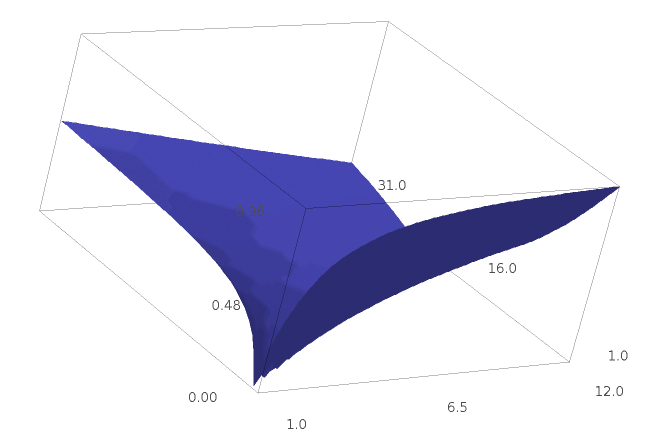
\includegraphics[height=2in]{rcbday.jpg}
          \end{center}
        \item We want to maximize this.
          \begin{equation*}
            \theta
            =
            \arccos(\,\frac{\colvec[r]{7 \\ 12}\dotprod\colvec{m \\ d}}{
                  \absval{\colvec[r]{7 \\ 12}\,}\cdot\absval{\colvec{m \\ d}\,} }\,)
          \end{equation*}
          Of course, we cannot take $m$ or $d$ negative and so we cannot
          get a vector orthogonal to the given one.
          This Python script finds the largest angle by brute force.
\begin{lstlisting}
  import math
  days={1:31,  # Jan
        2:29, 3:31, 4:30, 5:31, 6:30, 7:31, 8:31, 9:30, 10:31, 11:30, 12:31}
  BDAY=(7,12)
  max_res=0
  max_res_date=(-1,-1)
  for month in range(1,13):
      for day in range(1,days[month]+1):
          num=BDAY[0]*month+BDAY[1]*day
          denom=math.sqrt(BDAY[0]**2+BDAY[1]**2)*math.sqrt(month**2+day**2)
          if denom>0:
              res=math.acos(min(num*1.0/denom,1))
              print "day:",str(month),str(day)," angle:",str(res)
              if res>max_res:
                  max_res=res
                  max_res_date=(month,day)
  print "For ",str(BDAY),"worst case",str(max_res),"rads, date",str(max_res_date)
  print "  That is ",180*max_res/math.pi,"degrees"
\end{lstlisting}
          The result is 
\begin{lstlisting}
  For  (7, 12) worst case 0.95958064648 rads, date (12, 1)
    That is  54.9799211457 degrees
\end{lstlisting}

          A more conceptual approach is to consider the relation of all points 
          $(\text{month},\text{day})$ to the point $(7,12)$.
          The picture below
          makes clear that the answer is either Dec~$1$ or Jan~$31$, depending
          on which is further from the birthdate. 
          The dashed line bisects the angle between the line from the
          origin to Dec~$1$, and the line from the origin to Jan~$31$.
          Birthdays above the line are furthest from Dec~$1$ and 
          birthdays below the line are furthest from Jan~$31$.
          \begin{center}
            \includegraphics{ch1.54}
          \end{center}
      \end{exparts}
    \end{answer}
  \puzzle \item 
    \cite{Monthly33p118}
    A ship is sailing with speed and direction \( \vec{v}_1 \); the wind blows
    apparently (judging by the vane on the mast) in the direction of a vector
    \( \vec{a} \); on changing the direction and speed of the ship from
    \( \vec{v}_1 \) to \( \vec{v}_2 \) the apparent wind is in the direction
    of a vector \( \vec{b} \).

    Find the vector velocity of the wind.
    \begin{answer}
      \answerasgiven %
      The actual velocity \( \vec{v} \) of the wind is the sum of the
      ship's velocity and the apparent velocity of the wind.
      Without loss of generality we may assume \( \vec{a} \) and
      \( \vec{b} \) to be unit vectors, and may write
      \begin{equation*}
         \vec{v}=\vec{v}_1+s\vec{a}=\vec{v}_2+t\vec{b}
      \end{equation*}
      where \( s \) and \( t \) are undetermined scalars.
      Take the dot product first by \( \vec{a} \) and then by \( \vec{b} \)
      to obtain
      \begin{align*}
         s-t\vec{a}\dotprod\vec{b}
         &=\vec{a}\dotprod(\vec{v}_2-\vec{v}_1)    \\
         s\vec{a}\dotprod\vec{b}-t
         &=\vec{b}\dotprod(\vec{v}_2-\vec{v}_1)
      \end{align*}
      Multiply the second by \( \vec{a}\dotprod\vec{b} \), 
      subtract the result from the first, and find
      \begin{equation*}
         s=
         \frac{[\vec{a}-(\vec{a}\dotprod\vec{b})\vec{b}]
                   \dotprod(\vec{v}_2-\vec{v}_1)
              }{1-(\vec{a}\dotprod\vec{b})^2}.
      \end{equation*}
      Substituting in the original displayed equation, we get
      \begin{equation*}
         \vec{v}=\vec{v}_1+
         \frac{[\vec{a}-(\vec{a}\dotprod\vec{b})\vec{b}]
                  \dotprod(\vec{v}_2-\vec{v}_1)
              \vec{a}}{1-(\vec{a}\dotprod\vec{b})^2}.
      \end{equation*}  
    \end{answer}
  \item  
     Verify the Cauchy-Schwarz inequality by first proving
     Lagrange's identity:
     \begin{equation*}
      \left(\sum_{1\leq j\leq n} a_jb_j \right)^2
      =
      \left(\sum_{1\leq j\leq n}a_j^2\right)
      \left(\sum_{1\leq j\leq n}b_j^2\right)
      -
      \sum_{1\leq k < j\leq n}(a_kb_j-a_jb_k)^2
     \end{equation*}
     and then noting that the final term is positive.
     % (Recall the meaning
     % \begin{equation*}
     %   \sum_{1\leq j\leq n}a_jb_j=
     %   a_1b_1+a_2b_2+\cdots+a_nb_n
     % \end{equation*}
     % and
     % \begin{equation*}
     %   \sum_{1\leq j\leq n}{a_j}^2=
     %   {a_1}^2+{a_2}^2+\cdots+{a_n}^2
     % \end{equation*}
     % of the \( \Sigma \) notation.)
     This result 
     is an improvement over Cauchy-Schwarz because it gives a formula for
     the difference between the two sides.
     Interpret that difference in \( \Re^2 \).
     \begin{answer}
       We use induction on \( n \).

       In the \( n=1 \) base case the identity reduces to
       \begin{equation*}
          (a_1b_1)^2=({a_1}^2)({b_1}^2)-0
       \end{equation*}
       and clearly holds.

       For the inductive step assume that 
       the formula holds for the \( 0 \), \ldots, \( n \) cases.
       We will show that it then holds in the \( n+1 \) case.
       Start with the right-hand side
       \begin{multline*}
         \bigl( \sum_{1\leq j\leq n+1}{a_j}^2\bigr)
         \bigl( \sum_{1\leq j\leq n+1}{b_j}^2\bigr)
         -
         \sum_{1\leq k<j\leq n+1}\bigl(a_kb_j-a_jb_k\bigr)^2  \\
       \begin{aligned}
         &=
         \bigl[ (\sum_{1\leq j\leq n}{a_j}^2)+{a_{n+1}}^2\bigr]
         \bigl[ (\sum_{1\leq j\leq n}{b_j}^2)+{b_{n+1}}^2\bigr]   \\     
         &\hbox{}\quad -
         \bigl[\sum_{1\leq k<j\leq n}\bigl(a_kb_j-a_jb_k\bigr)^2+
         \sum_{1\leq k\leq n}\bigl(a_kb_{n+1}-a_{n+1}b_k\bigr)^2  \bigr] \\
         &=
         \bigl( \sum_{1\leq j\leq n}{a_j}^2\bigr)
         \bigl( \sum_{1\leq j\leq n}{b_j}^2\bigr)
         +
         \sum_{1\leq j\leq n}{b_j}^2{a_{n+1}}^2                 
         +
         \sum_{1\leq j\leq n}{a_j}^2{b_{n+1}}^2
         +
         {a_{n+1}}^2{b_{n+1}}^2                                 \\
         &\hbox{}\qquad\hbox{} -
         \bigl[\sum_{1\leq k<j\leq n}\bigl(a_kb_j-a_jb_k\bigr)^2+
         \sum_{1\leq k\leq n}\bigl(a_kb_{n+1}-a_{n+1}b_k\bigr)^2  \bigr] \\
         &=
         \bigl( \sum_{1\leq j\leq n}{a_j}^2\bigr)
         \bigl( \sum_{1\leq j\leq n}{b_j}^2\bigr)
         -\sum_{1\leq k<j\leq n}\bigl(a_kb_j-a_jb_k\bigr)^2   \\   
         &\hbox{}\quad +
         \sum_{1\leq j\leq n}{b_j}^2{a_{n+1}}^2
         +
         \sum_{1\leq j\leq n}{a_j}^2{b_{n+1}}^2
         +
         {a_{n+1}}^2{b_{n+1}}^2                                 \\
         &\hbox{}\qquad\hbox{} -
         \sum_{1\leq k\leq n}\bigl(a_kb_{n+1}-a_{n+1}b_k\bigr)^2
        \end{aligned}
       \end{multline*}
       and apply the inductive hypothesis.
       \begin{align*}
         &=
         \bigl( \sum_{1\leq j\leq n}a_jb_j\bigr)^2              
         +
         \sum_{1\leq j\leq n}{b_j}^2{a_{n+1}}^2
         +
         \sum_{1\leq j\leq n}{a_j}^2{b_{n+1}}^2
         +
         {a_{n+1}}^2{b_{n+1}}^2                          \\              
         &\hbox{}\qquad\hbox{}-
         \bigl[\sum_{1\leq k\leq n}{a_k}^2{b_{n+1}}^2
           -2\sum_{1\leq k\leq n}a_kb_{n+1}a_{n+1}b_k
           +\sum_{1\leq k\leq n}{a_{n+1}}^2{b_k}^2\bigr]        \\
         &=
         \bigl( \sum_{1\leq j\leq n}a_jb_j\bigr)^2
         +2\bigl(\sum_{1\leq k\leq n}a_kb_{n+1}a_{n+1}b_k\bigr)
         +{a_{n+1}}^2{b_{n+1}}^2                                 \\
         &=
         \bigl[\bigl(\sum_{1\leq j\leq n}a_jb_j\bigr)+a_{n+1}b_{n+1}\bigr]^2
       \end{align*}
       to derive the left-hand side.  
   \end{answer}
\end{exercises}


% Chapter 1, Section 3 _Linear Algebra_ Jim Hefferon
%  http://joshua.smcvt.edu/linearalgebra
%  2001-Jun-09
\section{Reduced Echelon Form}
After developing the mechanics of Gauss's Method, 
we observed that it can be done in more than one way.
For example, from this matrix 
\begin{equation*}
    \begin{mat}[r]
       2  &2  \\
       4  &3
    \end{mat}
\end{equation*}
we could derive any of these three echelon form matrices.
\begin{equation*}
    \begin{mat}[r]
       2  &2  \\
       0  &-1
    \end{mat}
    \qquad
    \begin{mat}[r]
       1  &1  \\
       0  &-1
    \end{mat}
    \qquad
    \begin{mat}[r]
       2  &0  \\
       0  &-1
    \end{mat}
\end{equation*}
The first results from $-2\rho_1+\rho_2$.
The second comes from doing $(1/2)\rho_1$ and then $-4\rho_1+\rho_2$.
The third comes
from $-2\rho_1+\rho_2$ followed by $2\rho_2+\rho_1$
(after the first row combination the matrix is already in
echelon form so the second one is extra work 
but it is nonetheless a legal row operation).

The fact that echelon form 
is not unique raises questions.
Will any two echelon form versions of a linear system have the same number of
free variables?
If yes, 
will the two have exactly the same free variables?
In this section we will 
give a way to decide if one linear system 
can be derived from another by row operations.
The answers to both questions, both `yes',
will follow from this.








\subsection{Gauss-Jordan Reduction}%
% Gaussian elimination coupled with back-substitution
% solves linear systems but it is not the only method possible.
Here is an extension of Gauss's Method that has some advantages.

\begin{example} \label{exm:GJRedReadOffSol}
To solve
\begin{equation*}
  \begin{linsys}{3}
    x  &+  &y  &-  &2z  &=  &-2  \\
       &   &y  &+  &3z  &=  &7   \\
    x  &   &   &-  &z   &=  &-1  
  \end{linsys}
\end{equation*}
we can start as usual by reducing it to echelon form.
\begin{equation*}
  \grstep{-\rho_1+\rho_3}
    \begin{amat}[r]{3}
       1  &1  &-2 &-2  \\
       0  &1  &3  &7   \\
       0  &-1 &1  &1
    \end{amat}
  \grstep{\rho_2+\rho_3}
    \begin{amat}[r]{3}
       1  &1  &-2 &-2  \\
       0  &1  &3  &7   \\
       0  &0  &4  &8
    \end{amat}
\end{equation*}
We can keep going to a second stage
by making the leading entries into \( 1 \)'s
\begin{equation*}
    \grstep{(1/4)\rho_3}
    \begin{amat}[r]{3}
       1  &1  &-2 &-2  \\
       0  &1  &3  &7   \\
       0  &0  &1  &2
    \end{amat}
\end{equation*}
and then to a third stage that uses the leading entries 
to eliminate all of the other entries in each column 
by combining upwards.
\begin{equation*}
  \grstep[2\rho_3+\rho_1]{-3\rho_3+\rho_2}
    \begin{amat}[r]{3}
       1  &1  &0  &2   \\
       0  &1  &0  &1   \\
       0  &0  &1  &2
    \end{amat}
  \grstep{-\rho_2+\rho_1}
    \begin{amat}[r]{3}
       1  &0  &0  &1   \\
       0  &1  &0  &1   \\
       0  &0  &1  &2
    \end{amat}
\end{equation*}
The answer is \( x=1 \), \( y=1 \), and \( z=2 \).
\end{example}
%<*Pivoting>
Using one entry to clear out the rest of a column is
\definend{pivoting}\index{pivoting} on that entry.
%</Pivoting>

Note that the row combination operations in the first stage move left to right,
from column one to column three, 
while the combination operations in the third stage move right to left.

\begin{example}  \label{exm:GJRedReadOffSolTwo}
The middle stage operations that 
turn the leading entries into \( 1 \)'s
don't interact so we can combine multiple ones into a single step.
\begin{align*}
    \begin{amat}[r]{2}
       2   &1   &7   \\
       4   &-2  &6
    \end{amat}
  &\grstep{-2\rho_1+\rho_2}
  \begin{amat}[r]{2}
       2   &1   &7   \\
       0   &-4  &-8
    \end{amat}                                   \\
  &\grstep[(-1/4)\rho_2]{(1/2)\rho_1}
  \begin{amat}[r]{2}
       1   &1/2   &7/2   \\
       0   &1     &2
    \end{amat}                                    \\
  &\grstep{-(1/2)\rho_2+\rho_1}
  \begin{amat}[r]{2}
       1   &0   &5/2   \\
       0   &1   &2
    \end{amat}
\end{align*}
The answer is $x=5/2$ and $y=2$.
\end{example}

%<*GaussJordanReduction>
This extension of Gauss's Method is the 
\definend{Gauss-Jordan Method}\index{Gauss's Method!Gauss-Jordan Method} or 
\definend{Gauss-Jordan reduction}.\index{linear equation!solution of!Gauss-Jordan}\index{Gauss's Method!Gauss-Jordan}
%</GaussJordanReduction>
% It goes past echelon form to a more refined, more specialized,
% matrix form.

\begin{definition}\label{def:RedEchForm}
%<*df:RedEchForm>
A matrix or linear system is in
\definend{reduced echelon form\/}\index{echelon form!reduced}\index{reduced echelon form}
if, in addition to being in echelon form, each leading entry is a~$1$ 
and is the only nonzero entry in its column.
%</df:RedEchForm>
\end{definition}

\noindent
%<*CostRedEchForm>
The cost of using Gauss-Jordan reduction to solve a system 
is the additional arithmetic.
The benefit is that we can just read off the solution set
description.
%</CostRedEchForm>

In any echelon form system, reduced or not, we can read off 
when the system has an empty
solution set because there is a contradictory equation.
We can read off 
when the system has a one-element solution set because there is no
contradiction and every
variable is the leading variable in some row.
And, we can read off when the system has an infinite solution set because 
there is no contradiction and at least one variable is free.

However, in reduced echelon form we can read off not just the size of the  
solution set but also its description.
We have no trouble describing the solution set when it is empty, of course.
\nearbyexample{exm:GJRedReadOffSol} and~\ref{exm:GJRedReadOffSolTwo} 
show how in a single element solution set case the single element is
in the column of constants.
The next example shows how to read the parametrization
of an infinite solution set.

\begin{example}
\begin{multline*}
  \begin{amat}[r]{4}
     2  &6  &1  &2  &5  \\
     0  &3  &1  &4  &1  \\
     0  &3  &1  &2  &5
  \end{amat}
  \grstep{-\rho_2+\rho_3}
  \begin{amat}[r]{4}
     2  &6  &1  &2  &5  \\
     0  &3  &1  &4  &1  \\
     0  &0  &0  &-2 &4
  \end{amat}                                        \\
  \grstep[(1/3)\rho_2 \\ -(1/2)\rho_3]{(1/2)\rho_1}
  \repeatedgrstep[-\rho_3+\rho_1]{-(4/3)\rho_3+\rho_2}
  \repeatedgrstep{-3\rho_2+\rho_1}
  \begin{amat}[r]{4}
     1  &0  &-1/2  &0  &-9/2  \\
     0  &1  &1/3   &0  &3  \\
     0  &0  &0     &1  &-2
  \end{amat}
\end{multline*}
As a linear system this is 
\begin{equation*}
  \begin{linsys}{4}
     x_1  &&     &-&1/2x_3  &&   &= &-9/2  \\
          &&x_2  &+&1/3x_3  &&   &= &3  \\
          &&     &&        &{}\hspace{.5em}{}&x_4 &= &-2    
  \end{linsys}
\end{equation*}
so a solution set description is this.
\begin{equation*}  
  S=\set{\colvec{x_1 \\ x_2 \\ x_3 \\ x_4}
                        =\colvec[r]{-9/2 \\ 3 \\ 0 \\ -2}
                         +\colvec[r]{1/2 \\ -1/3 \\ 1 \\ 0}x_3
                        \suchthat x_3\in\Re}
\end{equation*}
\end{example}

Thus echelon form isn't some kind of one best form for systems.
Other forms, such as reduced echelon form, have advantages and
disadvantages.
Instead of picturing linear systems (and the associated matrices) 
as things we operate on, 
always directed toward the goal of echelon form, we can think of 
them as interrelated when
we can get from one to another by row operations.
The rest of this subsection develops this relationship.

\begin{lemma} \label{le:RowOpsRev}
%<*lm:RowOpsRev>
Elementary row operations are reversible.
%</lm:RowOpsRev>
\end{lemma}

\begin{proof}
%<*pf:RowOpsRev>
For any matrix \( A \),
the effect of swapping rows is reversed by swapping them back,
multiplying a row by a nonzero \( k \) is undone by multiplying by
$1/k$,
and adding a multiple of row \( i \) to row \( j \) (with $i\neq j$)
is undone by subtracting the same multiple of row \( i \) from row \( j \).
\begin{equation*}
      A
     \grstep{\rho_i\leftrightarrow\rho_j}
     \repeatedgrstep{\rho_j\leftrightarrow\rho_i}
      A
  \qquad
        A
     \grstep{k\rho_i}
     \repeatedgrstep{(1/k)\rho_i}
      A
  \qquad
        A
     \grstep{k\rho_i+\rho_j}
     \repeatedgrstep{-k\rho_i+\rho_j}
      A                          
\end{equation*}
%</pf:RowOpsRev>
(We need the $i\neq j$ condition;
see \nearbyexercise{exer:INotJMakesRowOpsRev}.)
\end{proof}

Again, the point of view that we are developing, supported now by the lemma,
is that the term `reduces to' is misleading:~where
\( A\longrightarrow B \), we shouldn't think of \( B \) as
after~\( A \) or simpler than~$A$.
Instead we should think of the two matrices as interrelated.
Below is a picture.
It shows the matrices from the start of this section and their
reduced echelon form version in a cluster, as
inter-reducible. 
\begin{center}  
  \includegraphics{ch1.28}
\end{center}

%<*EquivMatrices>
We say 
that matrices that reduce to each other are equivalent with respect
to the relationship of row reducibility.
The next result justifies this, using the definition of 
an equivalence.\appendrefs{equivalence relations}
%</EquivMatrices>

\begin{lemma} \label{lm:ReducesToIsEqRel}
%<*lm:ReducesToIsEqRel>
Between matrices, `reduces to' is an equivalence re\-la\-tion.
%</lm:ReducesToIsEqRel>
\end{lemma}

\begin{proof}
%<*pf:ReducesToIsEqRel0>
We must check the conditions
(i)~reflexivity, that any matrix reduces to itself,
(ii)~symmetry, that if \( A \) reduces to \( B \) then
   \( B \) reduces to \( A \),
and (iii)~transitivity, that if \( A \) reduces to \( B \) and
      \( B \) reduces to \( C \) then \( A \) reduces to
      \( C \).
%</pf:ReducesToIsEqRel0>

%<*pf:ReducesToIsEqRel1>
Reflexivity is easy; any  matrix reduces to itself in zero-many operations.

The relationship is symmetric by the prior lemma\Dash if
\( A \) reduces to \( B \) by some row operations
then also \( B \) reduces to \( A \) by reversing those operations.
%</pf:ReducesToIsEqRel1>

%<*pf:ReducesToIsEqRel2>
For transitivity, suppose that \( A \) reduces to \( B \) and
that \( B \) reduces to \( C \).
Following the reduction steps from $A \rightarrow\cdots\rightarrow B$
with those from  $B \rightarrow\cdots\rightarrow C$ 
gives a reduction from \( A \) to \( C \).
%</pf:ReducesToIsEqRel2>
\end{proof}

\begin{definition} \label{df:RowEquivalence}
%<*df:RowEquivalence>
Two matrices that are interreducible by elementary row operations
are \definend{row equivalent}.\index{matrix!row equivalence}%
\index{row equivalence}\index{equivalence relation!row equivalence}
%</df:RowEquivalence>
\end{definition}

%<*RowEquivalanceClasses>
The diagram below shows the collection of all matrices as a box.
Inside that box each matrix lies in a class.
Matrices are in the same class if and only if they are interreducible.
The classes are disjoint\Dash no matrix is in two distinct classes.
We have partitioned the collection of matrices into 
\definend{row equivalence classes}.\appendrefs{partitions and class representatives}\index{partition!row equivalence classes}
%</RowEquivalanceClasses>
\begin{center}
  \includegraphics{ch1.27}
\end{center}
\noindent One of the classes is the
cluster of interrelated 
matrices from the start of this section pictured earlier,
expanded to include all of the nonsingular $\nbyn{2}$ matrices. 

The next subsection proves that the reduced echelon form of a matrix is 
unique.
Rephrased in terms of the row-equivalence relationship, 
we shall prove that every matrix is 
row equivalent to one and only one reduced echelon form matrix.
In terms of the partition what we shall prove is:~every
equivalence class contains one and only one reduced echelon form matrix.
So each reduced echelon form matrix serves as a representative of its 
class.

\begin{exercises}
   \recommended \item 
     Use Gauss-Jordan reduction to solve each system.
     \begin{exparts*}
        \partsitem \(
          \begin{linsys}[t]{2}
               x  &+  &y  &=  &2  \\
               x  &-  &y  &=  &0  
          \end{linsys}   \)
        \partsitem \(
          \begin{linsys}[t]{3}
               x  &   &   &-  &z  &=  &4  \\
              2x  &+  &2y &   &   &=  &1  
          \end{linsys}  \)
        \partsitem  \(
           \begin{linsys}[t]{2}
               3x  &-  &2y  &=  &1  \\
               6x  &+  &y   &=  &1/2 
           \end{linsys}  \)
        \partsitem \(
           \begin{linsys}[t]{3}
              2x  &-  &y  &  &  &= &-1  \\
               x  &+  &3y &- &z &= &5   \\
                  &   &y  &+ &2z&= &5   
           \end{linsys} \)
     \end{exparts*}
     \begin{answer}
       These answers show only the Gauss-Jordan reduction.
       With it, describing the solution set is easy. 
       \begin{exparts}
         \partsitem The solution set contains only a single element.
           \begin{multline*}
             \begin{amat}[r]{2}
               1  &1  &2  \\
               1  &-1 &0
             \end{amat}
             \grstep{-\rho_1+\rho_2}
             \begin{amat}[r]{2}
               1  &1  &2  \\
               0  &-2 &-2
             \end{amat}                          \\                       
             \grstep{-(1/2)\rho_2}
             \begin{amat}[r]{2}
               1  &1  &2  \\
               0  &1  &1
             \end{amat}                         
             \grstep{-\rho_2+\rho_1}
             \begin{amat}[r]{2}
               1  &0  &1  \\
               0  &1  &1
             \end{amat}
           \end{multline*}
         \partsitem The solution set has one parameter.
            \begin{equation*}
             \begin{amat}[r]{3}
               1  &0  &-1  &4  \\
               2  &2  &0   &1
             \end{amat}
             \grstep{-2\rho_1+\rho_2}
             \begin{amat}[r]{3}
               1  &0  &-1  &4  \\
               0  &2  &2   &-7
             \end{amat}                    
             \grstep{(1/2)\rho_2}
             \begin{amat}[r]{3}
               1  &0  &-1  &4  \\
               0  &1  &1   &-7/2
             \end{amat}
           \end{equation*}
         \partsitem There is a unique solution.
           \begin{multline*}
             \begin{amat}[r]{2}
               3  &-2  &1  \\
               6  &1   &1/2
             \end{amat}
             \grstep{-2\rho_1+\rho_2}
             \begin{amat}[r]{2}
               3  &-2  &1  \\
               0  &5   &-3/2
             \end{amat}                            \\                       
             \grstep[(1/5)\rho_2]{(1/3)\rho_1}
             \begin{amat}[r]{2}
               1  &-2/3&1/3 \\
               0  &1   &-3/10
             \end{amat}                       
             \grstep{(2/3)\rho_2+\rho_1}
             \begin{amat}[r]{2}
               1  &0   &2/15 \\
               0  &1   &-3/10
             \end{amat}
          \end{multline*}
        \partsitem A row swap in the second step makes the arithmetic easier.
         \begin{multline*}
          \begin{amat}[r]{3}
            2  &-1  &0  &-1  \\
            1  &3   &-1 &5   \\
            0  &1   &2  &5
          \end{amat}
          \grstep{-(1/2)\rho_1+\rho_2}
          \begin{amat}[r]{3}
            2  &-1  &0  &-1   \\
            0  &7/2 &-1 &11/2 \\
            0  &1   &2  &5
          \end{amat}                                \\
          \begin{aligned}
          &\grstep{\rho_2\leftrightarrow\rho_3}
          \begin{amat}[r]{3}
            2  &-1  &0  &-1   \\
            0  &1   &2  &5    \\
            0  &7/2 &-1 &11/2
          \end{amat}                      
            \grstep{-(7/2)\rho_2+\rho_3}
            \begin{amat}[r]{3}
              2  &-1  &0  &-1   \\
              0  &1   &2  &5    \\
              0  &0   &-8 &-12
            \end{amat}                               \\     
            &\grstep[-(1/8)\rho_2]{(1/2)\rho_1}
            \begin{amat}[r]{3}
              1  &-1/2&0  &-1/2 \\
              0  &1   &2  &5    \\
              0  &0   &1  &3/2
            \end{amat}                                
            \grstep{-2\rho_3+\rho_2}
            \begin{amat}[r]{3}
              1  &-1/2&0  &-1/2 \\
              0  &1   &0  &2    \\
              0  &0   &1  &3/2
            \end{amat}                                    \\             
            &\grstep{(1/2)\rho_2+\rho_1}
            \begin{amat}[r]{3}
              1  &0   &0  &1/2  \\
              0  &1   &0  &2    \\
              0  &0   &1  &3/2
            \end{amat}
          \end{aligned}
        \end{multline*}
       \end{exparts}  
     \end{answer}
  \item Do Gauss-Jordan reduction.
    \begin{exparts*}
      \partsitem
        $\begin{linsys}[t]{3}
          x  &+ &y &- &z &= &3 \\
          2x &- &y  &- &z &= &1 \\
          3x &+  &y  &+ &2z &= &0
        \end{linsys}$
      \partsitem
        $\begin{linsys}[t]{3}
          x  &+ &y  &+ &2z  &= &0 \\
          2x  &- &y  &+  &z &= &1 \\
          4x &+ &y  &+ &5z &= &1  
        \end{linsys}$
    \end{exparts*}
    \begin{answer}
      \begin{exparts}
        \partsitem
          \begin{multline*}
            \begin{amat}{3}
              1 &1  &-1 &3 \\
              2 &-1 &-1 &1 \\
              3 &1  &2  &0
            \end{amat}
            \grstep[-3\rho_1+\rho_3]{-2\rho_1+\rho_2}
            \begin{amat}{3}
              1 &1  &-1 &3 \\
              0 &-3 &1  &-5 \\
              0 &-2  &5  &-9
            \end{amat}                             \\
          \begin{aligned}   
            &\grstep{-(2/3)\rho_2+\rho_3}
            \begin{amat}{3}
              1 &1  &-1    &3 \\
              0 &-3 &1     &-5 \\
              0 &0  &13/3  &-17/3
            \end{amat}                                 
            \grstep[(3/13)\rho_3]{-(1/3)\rho_2}
            \begin{amat}{3}
              1 &1  &-1    &3 \\
              0 &1  &-1/3    &5/3 \\
              0 &0  &1      &-17/13
            \end{amat}                                \\
            &\grstep[(1/3)\rho_3+\rho_2]{\rho_3+\rho_1}
            \begin{amat}{3}
              1 &1  &0    &22/13 \\
              0 &1  &0    &16/13 \\
              0 &0  &1      &-17/13
            \end{amat}
            \grstep{-\rho_2+\rho_1}
            \begin{amat}{3}
              1 &0  &0    &6/13 \\
              0 &1  &0    &16/13 \\
              0 &0  &1      &-17/13
            \end{amat}
          \end{aligned}
          \end{multline*}
        \partsitem
          \begin{multline*}
            \begin{amat}{3}
              1 &1  &2 &0 \\
              2 &-1 &1 &1 \\
              4 &1  &5 &1
            \end{amat}
            \grstep[-4\rho_1+\rho_3]{-2\rho_1+\rho_2}
            \begin{amat}{3}
              1 &1  &2  &0 \\
              0 &-3 &-3 &1 \\
              0 &-3 &-3 &1
            \end{amat}
            \grstep{-\rho_2+\rho_3}
            \begin{amat}{3}
              1 &1  &2  &0 \\
              0 &-3 &-3 &1 \\
              0 &0  &0  &0
            \end{amat}                              \\
            \grstep{-(1/3)\rho_2}
            \begin{amat}{3}
              1 &1  &2  &0 \\
              0 &1  &1 &-1/3 \\
              0 &0  &0  &0
            \end{amat}
            \grstep{-\rho_2+\rho_1}
            \begin{amat}{3}
              1 &0  &1  &1/3 \\
              0 &1  &1 &-1/3 \\
              0 &0  &0  &0
            \end{amat}
          \end{multline*}
      \end{exparts}
    \end{answer}
  \recommended \item 
    Find the reduced echelon form of each matrix.
    \begin{exparts*}
      \partsitem \( \begin{mat}[r]
          2  &1  \\
          1  &3
        \end{mat}  \)
      \partsitem \( \begin{mat}[r]
          1  &3  &1  \\
          2  &0  &4  \\
         -1  &-3 &-3
        \end{mat}  \)
      \partsitem \( \begin{mat}[r]
          1  &0  &3  &1  &2  \\
          1  &4  &2  &1  &5  \\
          3  &4  &8  &1  &2
        \end{mat}  \)
      \partsitem \( \begin{mat}[r]
          0  &1  &3  &2  \\
          0  &0  &5  &6  \\
          1  &5  &1  &5
        \end{mat}  \)
    \end{exparts*}
    \begin{answer}
      Use Gauss-Jordan reduction.
      \begin{exparts}
        \partsitem The reduced echelon form is all zeroes except
          for a diagonal of ones.
          \begin{equation*}
            \grstep{-(1/2)\rho_1+\rho_2}
            \begin{mat}[r]
              2  &1  \\
              0  &5/2
            \end{mat}
            \grstep[(2/5)\rho_2]{(1/2)\rho_1}
            \begin{mat}[r]
              1  &1/2\\
              0  &1
            \end{mat}                      
            \grstep{-(1/2)\rho_2+\rho_1}
            \begin{mat}[r]
              1  &0  \\
              0  &1
            \end{mat}
          \end{equation*}
        \partsitem As in the prior problem, the reduced echelon form is 
          all zeroes but for a diagonal of ones.
          \begin{multline*}
            \grstep[\rho_1+\rho_3]{-2\rho_1+\rho_2}
            \begin{mat}[r]
              1  &3  &1  \\
              0  &-6 &2  \\
              0  &0  &-2
            \end{mat}
            \grstep[-(1/2)\rho_3]{-(1/6)\rho_2}
            \begin{mat}[r]
              1  &3  &1     \\
              0  &1  &-1/3  \\
              0  &0  &1
            \end{mat}                                      \\              
            \grstep[-\rho_3+\rho_1]{(1/3)\rho_3+\rho_2}
            \begin{mat}[r]
              1  &3  &0     \\
              0  &1  &0     \\
              0  &0  &1
            \end{mat}                  
            \grstep{-3\rho_2+\rho_1}
            \begin{mat}[r]
              1  &0  &0     \\
              0  &1  &0     \\
              0  &0  &1
            \end{mat}
           \end{multline*}
        \partsitem There are more columns than rows so we must get more
          than just a diagonal of ones.
          \begin{multline*}
            \grstep[-3\rho_1+\rho_3]{-\rho_1+\rho_2}
            \begin{mat}[r]
              1  &0  &3  &1  &2  \\
              0  &4  &-1 &0  &3  \\
              0  &4  &-1 &-2 &-4
            \end{mat}
            \grstep{-\rho_2+\rho_3}
            \begin{mat}[r]
              1  &0  &3  &1  &2  \\
              0  &4  &-1 &0  &3  \\
              0  &0  &0  &-2 &-7
            \end{mat}                           \\
            \grstep[-(1/2)\rho_3]{(1/4)\rho_2}
            \begin{mat}[r]
              1  &0  &3    &1  &2  \\
              0  &1  &-1/4 &0  &3/4  \\
              0  &0  &0    &1  &7/2
            \end{mat}                           
            \grstep{-\rho_3+\rho_1}
            \begin{mat}[r]
              1  &0  &3    &0  &-3/2  \\
              0  &1  &-1/4 &0  &3/4     \\
              0  &0  &0    &1  &7/2
            \end{mat}
          \end{multline*}
        \partsitem As in the prior item, this is not a square matrix. 
          \begin{multline*}
            \grstep{\rho_1\leftrightarrow\rho_3}
            \begin{mat}[r]
              1  &5  &1  &5  \\
              0  &0  &5  &6  \\
              0  &1  &3  &2
            \end{mat}
            \grstep{\rho_2\leftrightarrow\rho_3}
            \begin{mat}[r]
              1  &5  &1  &5  \\
              0  &1  &3  &2  \\
              0  &0  &5  &6
            \end{mat}                    \\
            \begin{aligned}
              &\grstep{(1/5)\rho_3}
              \begin{mat}[r]
                1  &5  &1  &5  \\
                0  &1  &3  &2  \\
                0  &0  &1  &6/5
              \end{mat}                  
              \grstep[-\rho_3+\rho_1]{-3\rho_3+\rho_2}
              \begin{mat}[r]
                1  &5  &0  &19/5  \\
                0  &1  &0  &-8/5  \\
                0  &0  &1  &6/5
              \end{mat}                   \\
              &\grstep{-5\rho_2+\rho_1}
              \begin{mat}[r]
                1  &0  &0  &59/5  \\
                0  &1  &0  &-8/5  \\
                0  &0  &1  &6/5
              \end{mat}
            \end{aligned}
          \end{multline*}
      \end{exparts}  
    \end{answer}
  \item Get the reduced echelon form of each.
    \begin{exparts*}
      \partsitem $
        \begin{mat}
          0  &2 &1 \\
          2  &-1 &1 \\
          -2 &-1 &0
        \end{mat}$
      \partsitem $
        \begin{mat}
          1 &3 &1 \\
          2 &6 &2 \\
         -1 &0 &0
        \end{mat}$
    \end{exparts*}
    \begin{answer}
      \begin{exparts}
        \partsitem Swap first.
          \begin{equation*}
            \grstep{\rho_1\leftrightarrow\rho_2}
            \grstep{\rho_1+\rho_3}
            \grstep{\rho_2+\rho_3}
            \grstep[(1/2)\rho_2 \\ (1/2)\rho_3]{(1/2)\rho_1}
            \grstep[(-1/2)\rho_3+\rho_2]{(-1/2)\rho_3+\rho_1}
            \grstep{(1/2)\rho_2+\rho_1}
            \begin{mat}
              1 &0 &0 \\
              0 &1 &0 \\
              0 &0 &1
            \end{mat}
          \end{equation*}
        \partsitem Here the swap is in the middle.
        \begin{equation*}
          \grstep[\rho_1+\rho_3]{-2\rho_1+\rho_2}
          \grstep{\rho_2\leftrightarrow\rho_3}
          \grstep{(1/3)\rho_2}
          \grstep{-3\rho_2+\rho_1}
          \begin{mat}
            1 &0 &0   \\
            0 &1 &1/3 \\
            0 &0 &0
          \end{mat}
        \end{equation*}
      \end{exparts}
    \end{answer}
  \recommended \item 
    Find each solution set by using Gauss-Jordan reduction and
    then reading off the parametrization.
    \begin{exparts}
      \partsitem \( \begin{linsys}[t]{3}
                  2x  &+  &y  &-  &z  &=  &1  \\
                  4x  &-  &y  &   &   &=  &3  
                  \end{linsys}  \)
      \partsitem \( \begin{linsys}[t]{4}
                   x  &   &   &-  &z  &   &   &=  &1  \\
                      &   &y  &+  &2z &-  &w  &=  &3  \\
                   x  &+  &2y &+  &3z &-  &w  &=  &7  
                    \end{linsys}  \)
      \partsitem \( \begin{linsys}[t]{4}
                   x  &-  &y  &+  &z  &   &   &=  &0  \\
                      &   &y  &   &   &+  &w  &=  &0  \\
                  3x  &-  &2y &+  &3z &+  &w  &=  &0  \\
                      &   &-y &   &   &-  &w  &=  &0  
                  \end{linsys}  \)
      \partsitem \( \begin{linsys}[t]{5}
                   a  &+  &2b &+  &3c &+  &d  &-  &e  &=  &1  \\
                  3a  &-  &b  &+  &c  &+  &d  &+  &e  &=  &3  
                  \end{linsys}  \)
    \end{exparts}
    \begin{answer}
      For the Gauss's halves, see the answers to Chapter One's
      section~I.2 question
      \nearbyexercise{exer:SlvMatNot}.
      \begin{exparts}
      \partsitem The ``Jordan'' half goes this way.
        \begin{equation*}
          \grstep[-(1/3)\rho_2]{(1/2)\rho_1}
          \begin{amat}[r]{3}
            1  &1/2 &-1/2 &1/2  \\
            0  &1   &-2/3 &-1/3
          \end{amat}                           
          \grstep{-(1/2)\rho_2+\rho_1}
          \begin{amat}[r]{3}
            1  &0   &-1/6 &2/3  \\
            0  &1   &-2/3 &-1/3
          \end{amat}
        \end{equation*}
        The solution set is this
        \begin{equation*}
          \set{\colvec[r]{2/3 \\ -1/3 \\ 0}
               +\colvec[r]{1/6 \\ 2/3 \\ 1}z
              \suchthat z\in\Re}
        \end{equation*}
      \partsitem The second half is
        \begin{equation*}
          \grstep{\rho_3+\rho_2}
          \begin{amat}[r]{4}
            1  &0  &-1  &0  &1 \\
            0  &1  &2   &0  &3 \\
            0  &0  &0   &1  &0
          \end{amat}
        \end{equation*}
        so the solution is this.
        \begin{equation*}
          \set{\colvec[r]{1 \\ 3 \\ 0 \\ 0}
               +\colvec[r]{1 \\ -2 \\ 1 \\ 0}z
              \suchthat z\in\Re}
        \end{equation*}
      \partsitem This Jordan half
        \begin{equation*}
          \grstep{\rho_2+\rho_1}
          \begin{amat}[r]{4}
            1  &0  &1   &1  &0 \\
            0  &1  &0   &1  &0 \\
            0  &0  &0   &0  &0 \\
            0  &0  &0   &0  &0
          \end{amat}
        \end{equation*}
        gives 
        \begin{equation*}
          \set{\colvec[r]{0 \\ 0 \\ 0 \\ 0}
               +\colvec[r]{-1 \\ 0 \\ 1 \\ 0}z
               +\colvec[r]{-1 \\ -1 \\ 0 \\ 1}w
              \suchthat z,w\in\Re}
        \end{equation*}
        (of course, we could omit the zero vector from the description).
      \partsitem The ``Jordan'' half
        \begin{align*}
          &\grstep{-(1/7)\rho_2}
          \begin{amat}[r]{5}
            1  &2  &3   &1   &-1   &1  \\
            0  &1  &8/7 &2/7 &-4/7 &0
          \end{amat}                   \\
          &\grstep{-2\rho_2+\rho_1}
          \begin{amat}[r]{5}
            1  &0  &5/7 &3/7 &1/7  &1  \\
            0  &1  &8/7 &2/7 &-4/7 &0
          \end{amat}
        \end{align*}
        ends with this solution set.
        \begin{equation*}
          \set{\colvec[r]{1 \\ 0 \\ 0 \\ 0 \\ 0}
               +\colvec[r]{-5/7 \\ -8/7 \\ 1 \\ 0 \\ 0}c
               +\colvec[r]{-3/7 \\ -2/7 \\ 0 \\ 1 \\ 0}d
               +\colvec[r]{-1/7 \\ 4/7 \\ 0 \\ 0 \\ 1}e
              \suchthat c,d,e\in\Re}
        \end{equation*}
    \end{exparts}
   \end{answer}
  \item 
    Give two distinct echelon form versions of this matrix.
    \begin{equation*}
      \begin{mat}[r]
        2  &1  &1  &3  \\
        6  &4  &1  &2  \\
        1  &5  &1  &5
      \end{mat}
    \end{equation*}
    \begin{answer}
      Routine Gauss's Method gives one:
      \begin{equation*}
        \grstep[-(1/2)\rho_1+\rho_3]{-3\rho_1+\rho_2}
        \begin{mat}[r]
          2  &1  &1  &3  \\
          0  &1  &-2 &-7 \\
          0  &9/2&1/2&7/2
        \end{mat}
        \grstep{-(9/2)\rho_2+\rho_3}
        \begin{mat}[r]
          2  &1  &1    &3  \\
          0  &1  &-2   &-7 \\
          0  &0  &19/2 &35
        \end{mat}
      \end{equation*}
      and any cosmetic change, such as multiplying the bottom row by \( 2 \),
      \begin{equation*}
        \begin{mat}[r]
          2  &1  &1    &3  \\
          0  &1  &-2   &-7 \\
          0  &0  &19   &70
        \end{mat}
      \end{equation*}
      gives another.  
    \end{answer}
  \recommended \item \label{exer:PossRedEchFrms} 
    List the reduced echelon forms possible for each size.
    \begin{exparts*}
      \partsitem \( \nbyn{2} \)
      \partsitem \( \nbym{2}{3} \)
      \partsitem \( \nbym{3}{2} \)
      \partsitem \( \nbyn{3} \)
    \end{exparts*}
    \begin{answer}
      In the cases listed below, we take $a,b\in\Re$.
      Thus, some canonical forms 
      listed below actually include infinitely many cases.
      In particular, they includes the cases $a=0$ and $b=0$.
      \begin{exparts}
        \partsitem 
          $\begin{mat}[r]
            0  &0  \\
            0  &0
          \end{mat}$,
          $\begin{mat}[r]
            1  &a  \\
            0  &0
          \end{mat}$, 
          $\begin{mat}[r]
            0  &1  \\
            0  &0
          \end{mat}$, 
          $\begin{mat}[r]
            1  &0  \\
            0  &1
          \end{mat}$
        \partsitem
          $\begin{mat}[r]
               0  &0  &0  \\
               0  &0  &0
             \end{mat}$,
          $\begin{mat}[r]
               1  &a  &b  \\
               0  &0  &0
             \end{mat}$,
          $\begin{mat}[r]
               0  &1  &a  \\
               0  &0  &0
             \end{mat}$,
          $\begin{mat}[r]
               0  &0  &1  \\
               0  &0  &0
             \end{mat}$,
          $\begin{mat}[r]
               1  &0  &a  \\
               0  &1  &b
             \end{mat}$,
          $\begin{mat}[r]
               1  &a  &0  \\
               0  &0  &1
             \end{mat}$,
          $\begin{mat}[r]
               0  &1  &0  \\
               0  &0  &1
             \end{mat}$
        \partsitem
          $\begin{mat}[r]
               0  &0  \\
               0  &0  \\
               0  &0
             \end{mat}$,
          $\begin{mat}[r]
               1  &a  \\
               0  &0  \\
               0  &0
             \end{mat}$,
          $\begin{mat}[r]
               0  &1  \\
               0  &0  \\
               0  &0
             \end{mat}$,
          $\begin{mat}[r]
               1  &0  \\
               0  &1  \\
               0  &0
             \end{mat}$
        \partsitem
          $\begin{mat}[r]
               0  &0  &0  \\
               0  &0  &0  \\
               0  &0  &0
             \end{mat}$,
          $\begin{mat}[r]
               1  &a  &b  \\
               0  &0  &0  \\
               0  &0  &0
             \end{mat}$,
          $\begin{mat}[r]
               0  &1  &a  \\
               0  &0  &0  \\
               0  &0  &0
             \end{mat}$,
          $\begin{mat}[r]
               0  &1  &0  \\
               0  &0  &1  \\
               0  &0  &0
             \end{mat}$,
          $\begin{mat}[r]
               0  &0  &1  \\
               0  &0  &0  \\
               0  &0  &0
             \end{mat}$,
          $\begin{mat}[r]
               1  &0  &a  \\
               0  &1  &b  \\
               0  &0  &0
             \end{mat}$,
          $\begin{mat}[r]
               1  &a  &0  \\
               0  &0  &1  \\
               0  &0  &0
             \end{mat}$,
          $\begin{mat}[r]
               1  &0  &0  \\
               0  &1  &0  \\
               0  &0  &1
             \end{mat}$
      \end{exparts}  
    \end{answer}
  \recommended \item  
    What results from applying Gauss-Jordan reduction to a
    nonsingular matrix?
    \begin{answer}
      A nonsingular homogeneous linear system has a unique solution.
      So a nonsingular matrix must reduce to a (square) 
      matrix that is all \( 0 \)'s
      except for \( 1 \)'s down the upper-left to lower-right diagonal, 
      such as these.
      \begin{equation*}
         \begin{mat}[r]
           1  &0  \\
           0  &1  \\
         \end{mat}
         \qquad
         \begin{mat}[r]
           1  &0  &0  \\
           0  &1  &0  \\
           0  &0  &1
         \end{mat}
      \end{equation*}  
    \end{answer}
 \item \cite{Cleary}
    Consider the following relationship on the set of $\nbyn{2}$ matrices:  
    we say that $A$ is \textit{sum-what like} $B$ if the sum of all of 
    the entries in $A$ is the same as the sum of all the entries in $B$.  
    For instance, the zero matrix would be sum-what like the matrix 
    whose first row had two sevens, and whose second row had two 
    negative sevens.
    Prove or disprove that this is an equivalence relation on the set 
    of $\nbyn{2}$ matrices.
    \begin{answer}
      It is an equivalence relation.
      To prove that we must check that the relation 
      is reflexive, symmetric, and transitive.

      Assume that all matrices are $\nbyn{2}$.
      For reflexive, we note that a matrix has the same sum of entries as
      itself.
      For symmetric, we assume $A$ has the same sum of entries as~$B$ 
      and obviously then $B$ has the same sum of entries as~$A$.
      Transitivity is no harder\Dash if $A$ has the same sum of entries
      as $B$ and $B$ has the same sum of entries as $C$ then 
      $A$ has the same as $C$.
    \end{answer}
 \item \label{exer:INotJMakesRowOpsRev}
   The proof of \nearbylemma{le:RowOpsRev} contains a reference to the 
   $i\neq j$ condition on the row combination operation.
   \begin{exparts}
     \partsitem Write down a $\nbyn{2}$ matrix with nonzero entries,
        and show that the $-1\cdot\rho_1+\rho_1$ operation is not
        reversed by $1\cdot\rho_1+\rho_1$.
     \partsitem Expand the proof of that lemma to make explicit exactly where 
        it uses the $i\neq j$ condition on combining.
   \end{exparts}
   \begin{answer}
    \begin{exparts}
      \partsitem For instance,
        \begin{equation*}
          \begin{mat}[r]
            1  &2  \\
            3  &4  
          \end{mat}
          \grstep{-\rho_1+\rho_1}
          \begin{mat}[r]
            0  &0  \\
            3  &4  
          \end{mat}
          \grstep{\rho_1+\rho_1}
          \begin{mat}[r]
            0  &0  \\
            3  &4  
          \end{mat}
        \end{equation*}
        leaves the matrix changed.
      \partsitem This operation
        \begin{equation*}
          \begin{mat}
            \vdotswithin{a_{i,1}}                     \\
            a_{i,1}  &\cdots  &a_{i,n}  \\
            \vdotswithin{a_{i,1}}                     \\
            a_{j,1}  &\cdots  &a_{j,n}  \\
            \vdotswithin{a_{i,1}}                     
          \end{mat}
          \grstep{k\rho_i+\rho_j}
          \begin{mat}
            \vdotswithin{a_{i,1}}                                      \\
            a_{i,1}           &\cdots  &a_{i,n}          \\
            \vdotswithin{a_{i,1}}                                      \\
            ka_{i,1}+a_{j,1}  &\cdots  &ka_{i,n}+a_{j,n}  \\
            \vdotswithin{a_{i,1}}                     
          \end{mat}
        \end{equation*}      
        leaves the $i$-th row unchanged because of the $i\neq j$ restriction.
        Because the $i$-th row is unchanged, this operation 
        \begin{equation*}                                        
          \grstep{-k\rho_i+\rho_j}
          \begin{mat}
            \vdotswithin{a_{i,1}}                                      \\
            a_{i,1}           &\cdots  &a_{i,n}          \\
            \vdotswithin{a_{i,1}}                                      \\
            -ka_{i,1}+ka_{i,1}+a_{j,1}  &\cdots &-ka_{i,n}+ka_{i,n}+a_{j,n} \\
            \vdotswithin{a_{i,1}}                     
          \end{mat}
        \end{equation*}
        returns the $j$-th row to its original state.
        % (If $i=j$ then the third matrix would have entries of the 
        % form $-k(ka_{i,j}+a_{i,j})+ka_{i,j}+a_{i,j}$.)
    \end{exparts}
   \end{answer}
 \item \cite{Cleary}
  Consider the set of students in a class.  
  Which of the following relationships are equivalence relations?  
  Explain each answer in at least a sentence.
  \begin{exparts}
    \item  Two students $x, y$ are related 
      if $x$ has taken at least as many 
      math classes as $y$.
    \item Students $x, y$ are related if they have names 
      that start with the same letter.
  \end{exparts}
  \begin{answer}
    To be an equivalence, each relation must be reflexive, symmetric, and
    transitive.
    \begin{exparts}
      \item This relation 
        is not symmetric because if $x$ has taken $4$~classes and $y$
        has taken $3$ then $x$ is related to $y$ but $y$ is not related
        to $x$.
      \item This is reflexive because $x$'s name starts with the same
        letter as does $x$'s.
        It is symmetric because if $x$'s name starts with the same letter 
        as $y$'s then $y$'s starts with the same letter as does~$x$'s.
        And it is transitive because if $x$'s name starts with the same letter
        as does~$y$'s and $y$'s name starts with the same letter as 
        does $z$'s then $x$'s starts with the same letter as does $z$'s.
        So it is an equivalence.
    \end{exparts}
  \end{answer}
  \item
  Show that each of these is an equivalence on the set of $\nbyn{2}$
  matrices.
  Describe the equivalence classes.
  \begin{exparts}
    \item Two matrices are related if they have the same product down the
      diagonal, that is, if the product of the entries in the upper left and
      lower right are equal.
    \item Two matrices are related if they both have at least one entry 
      that is a~$1$,
      or if neither does.
  \end{exparts}
  \begin{answer}
    For each we must check the three conditions of reflexivity, symmetry, and
    transitivity.
    \begin{exparts}
      \item Any matrix clearly has the same product down the diagonal as
        itself, so the relation is reflexive.
        The relation is symmetric because if $A$ has the same product down
        its diagonal as does~$B$,
        if $a_{1,1}\cdot a_{2,2}=b_{1,1}\cdot b_{2,2}$, 
        then $B$ has the same product as does~$A$.
 
        Transitivity is similar: suppose that $A$'s product is~$r$ and 
        that it equals $B$'s product.
        Suppose also that $B$'s product equals $C$'s.
        Then all three have a product of~$r$, and $A$'s equals~$C$'s.

        There is an equivalence class for each real number, namely the 
        class contains all $\nbyn{2}$ matrices whose product down the
        diagonal is that real.
      \item For reflexivity, if the matrix $A$ has a~$1$ entry then it is 
        related to itself while if it does not then it is also related to 
        itself.
        Symmetry also has two cases: suppose that $A$ and~$B$ are related.
        If $A$ has a~$1$ entry then so does~$B$, and thus $B$ is related to~$A$.
        If $A$ has no~$1$ then neither does $B$, and again $B$ is related to
        $A$.
 
        For transitivity, suppose that $A$ is related to~$B$ and $B$ to~$C$.
        If $A$ has a~$1$ entry then so does~$B$, and because $B$ is related
        to~$C$, therefore so does~$C$,
        and hence $A$ is related to~$C$.
        Likewise, if $A$ has no~$1$ then neither does~$B$, and consequently
        neither does~$C$, giving the conclusion that $A$ is related to~$C$. 

        There are exactly two equivalence classes, one containing any
        $\nbyn{2}$ matrix that has at least one entry that is a~$1$,
        and the other containing all the matrices that have no $1$'s.
    \end{exparts}
  \end{answer}
  \item Show that each is not an equivalence on the
    set of $\nbyn{2}$ matrices.
    \begin{exparts}
      \item Two matrices $A,B$ are related if $a_{1,1}=-b_{1,1}$.
      \item Two matrices are related if the sum of their entries are
        within $5$, that is, $A$ is related to~$B$ if
        $\absval{(a_{1,1}+\cdots+a_{2,2})-(b_{1,1}+\cdots+b_{2,2})}<5$.
    \end{exparts}
    \begin{answer}
      \begin{exparts}
        \item This relation is not reflexive.
          For instance, any matrix with an upper-left entry of~$1$ is not
          related to itself.
        \item This relation is not transitive.
          For these three, $A$ is related to~$B$, and $B$ is related to~$C$,
          but $A$ is not related to~$C$.
          \begin{equation*}
            A=\begin{mat}
              0 &0 \\
              0 &0
            \end{mat},\quad
            B=\begin{mat}
              4 &0 \\
              0 &0
            \end{mat},\quad
            C=\begin{mat}
              8 &0 \\
              0 &0
            \end{mat},\quad
          \end{equation*}
      \end{exparts}
    \end{answer}
\end{exercises}




















\subsection{The Linear Combination Lemma}
We will close this chapter by proving 
that every matrix is row equivalent to one
and only one reduced echelon form matrix.
The ideas here will reappear, and be further developed, in the
next chapter.
% Here is an informal argument that the reduced 
% echelon form version of a matrix is unique.
% Consider again the example that started this section of a matrix that
% reduces to three different echelon form matrices.
% The first matrix of the three is the natural echelon form version.
% The second matrix is the same as 
% the first except that a row has been halved.
% The third matrix, too, is just a cosmetic variant of the first. 
% The definition of reduced echelon form outlaws this kind of fooling around.
% In reduced echelon form,
% halving a row is not possible because that would
% change the row's leading entry away from one, and
% neither is combining rows possible, because then a leading entry would no
% longer be alone in its column.

% This informal justification is not a proof;
% the argument shows that no two different reduced echelon form matrices
% are related by a single row operation step, but the argument does not
% rule out the possibility that two different reduced echelon form
% matrices could be related by multiple steps.
% Before we go to the proof, we finish this subsection by 
% rephrasing our work in a terminology that will be enlightening.
The crucial observation concerns 
how row operations act to transform one matrix into another:
the new rows are
linear combinations of the old.

\begin{example}
Consider this Gauss-Jordan reduction.
\begin{align*}
  \begin{amat}{2}
    2  &1  &0  \\
    1  &3  &5
  \end{amat}
  &\grstep{-(1/2)\rho_1+\rho_2}
  \begin{amat}{2}
    2  &1    &0  \\
    0  &5/2  &5
  \end{amat}                           \\
  &\grstep[(2/5)\rho_2]{(1/2)\rho_1}
  \begin{amat}{2}
    1  &1/2  &0  \\
    0  &1    &2
  \end{amat}                        \\
  &\grstep{-(1/2)\rho_2+\rho_1}\;
  \begin{amat}{2}
    1  &0    &-1  \\
    0  &1    &2
  \end{amat}                       
\end{align*}
Denoting those matrices $A\rightarrow D\rightarrow G\rightarrow B$
and writing the rows of $A$ as $\alpha_1$ and $\alpha_2$, etc., we have this.
\begin{align*}  % multline looks worse
  \left(\begin{array}{l}
    \alpha_1 \\
    \alpha_2
  \end{array}\right)
  &\grstep{-(1/2)\rho_1+\rho_2}
  \left(\begin{array}{l}
    \delta_1=\alpha_1 \\
    \delta_2=-(1/2)\alpha_1+\alpha_2
  \end{array}\right)                          \\
  &\grstep[(2/5)\rho_2]{(1/2)\rho_1}
  \left(\begin{array}{l}
    \gamma_1=(1/2)\alpha_1 \\
    \gamma_2=-(1/5)\alpha_1+(2/5)\alpha_2
  \end{array}\right)                          \\
  &\grstep{-(1/2)\rho_2+\rho_1}
  \left(\begin{array}{l}
    \beta_1=(3/5)\alpha_1-(1/5)\alpha_2  \\
    \beta_2=-(1/5)\alpha_1+(2/5)\alpha_2
  \end{array}\right)                         
\end{align*} 
\end{example}

\begin{example}
The fact that Gaussian operations combine rows linearly 
also holds if there is a row swap.
With this \( A \), \( D \), \( G \), and \( B \)
\begin{equation*}
    \begin{mat}[r]
       0  &2  \\
       1  &1
     \end{mat}
    \grstep{\rho_1\leftrightarrow\rho_2}
    \begin{mat}[r]
       1  &1  \\
       0  &2
     \end{mat}                  
    \grstep{(1/2)\rho_2}
    \begin{mat}[r]
       1  &1  \\
       0  &1
     \end{mat}                   
    \grstep{-\rho_2+\rho_1}
    \begin{mat}[r]
       1  &0  \\
       0  &1
     \end{mat}
\end{equation*}
we get these linear
relationships. 
\begin{multline*}
  \left(\begin{array}{l}
    \vec{\alpha}_1 \\
    \vec{\alpha}_2
  \end{array}\right)
  \,\grstep{\rho_1\leftrightarrow\rho_2}\,
  \left(\begin{array}{l}
     \vec{\delta}_1 =\vec{\alpha}_2   \\
     \vec{\delta}_2 =\vec{\alpha}_1
  \end{array}\right)                                                 
  \,\grstep{(1/2)\rho_2}\,
  \left(\begin{array}{l}
     \vec{\gamma}_1 =\vec{\alpha}_2  \\
     \vec{\gamma}_2 =(1/2)\vec{\alpha}_1
  \end{array}\right)                                               \\
  \,\grstep{-\rho_2+\rho_1}\,
  \left(\begin{array}{l}
     \vec{\beta}_1 =(-1/2)\vec{\alpha}_1+1\cdot\vec{\alpha}_2   \\
     \vec{\beta}_2 =(1/2)\vec{\alpha}_1
  \end{array}\right)
\end{multline*}
\end{example}

In summary, 
Gauss's Method systematically finds a suitable 
sequence of linear combinations 
of the rows.

% \begin{definition}
% A \definend{linear combination}\index{linear combination} of 
% \( x_1,\ldots,x_m \)
% is an expression of the form $c_1x_1+c_2x_2+\,\cdots\,+c_mx_m$
% where the \( c \)'s are scalars.
%\end{definition}

% \noindent (We have already used the phrase 
% `linear combination' in this book.
% The meaning is unchanged, but the next result's statement makes
% a more formal definition in order.)

\begin{lemma}[Linear Combination Lemma] \label{lm:LinearCombinationLemma} \index{Linear Combination Lemma}
%<*lm:LinearCombinationLemma>
A linear combination of linear combinations is a linear combination.
%</lm:LinearCombinationLemma>
\end{lemma}

\begin{proof}
%<*pf:LinearCombinationLemma>
Given the set  
$c_{1,1}x_1+\dots+c_{1,n}x_n$ through $c_{m,1}x_1+\dots+c_{m,n}x_n$
of linear combinations of the $x$'s,
consider a combination of those
\begin{equation*}
  d_1(c_{1,1}x_1+\dots+c_{1,n}x_n)\,+\dots+\,d_m(c_{m,1}x_1+\dots+c_{m,n}x_n)
\end{equation*}
where the $d$'s are scalars along with the $c$'s.
Distributing those $d$'s and regrouping gives
\begin{equation*}
  %&=d_1c_{1,1}x_1+\dots+d_1c_{1,n}x_n\,
  % +d_2c_{2,1}x_1+\dots+\,
  % d_mc_{1,1}x_1+\dots+d_mc_{1,n}x_n         \\
  =(d_1c_{1,1}+\dots+d_mc_{m,1})x_1\,+\dots+\,(d_1c_{1,n}+\dots+d_mc_{m,n})x_n
\end{equation*}
which is also a linear combination of the $x$'s.
%</pf:LinearCombinationLemma>
\end{proof}


\begin{corollary} \label{cor:RowsOfEqMatsLinCombos}
%<*co:RowsOfEqMatsLinCombos>
Where one matrix reduces to another, each row of the second
is a linear combination of the rows of the first.
%</co:RowsOfEqMatsLinCombos>
\end{corollary}

% The proof 
% uses induction. % \appendrefs{mathematical induction}\spacefactor=1000 %
% Before we proceed, here is an outline of the argument.
% For the base step, we
% will verify that the proposition is true when reduction 
% can be done in zero row operations.
% For the inductive step, we will 
% argue that if being able to reduce the first matrix to the second in some
% number $t\geq 0$ of operations implies that each row of the second is a linear
% combination of the rows of the first, then being able to reduce the first to
% the second in $t+1$ operations implies the same thing.
% Together these prove the result because  
% the base step shows that it is true in the zero operations case,
% and then the inductive step
% implies that it is true in the one operation case, and then the inductive step
% applied again gives that it is therefore true for two operations, etc.

\begin{proof}
%<*pf:RowsOfEqMatsLinCombos0>
For any two interreducible matrices $A$ and~$B$ there is some
minimum number of row operations that will take one to the other.
We proceed by induction on that number. 

In the base step, that we can go from one matrix to another using
zero reduction operations, the two are equal.
Then each row of $B$ is trivially a combination of
$A$'s rows $\vec{\beta}_i
  =0\cdot\vec{\alpha}_1+\cdots+1\cdot\vec{\alpha}_i+\cdots+0\cdot\vec{\alpha}_m$.
%</pf:RowsOfEqMatsLinCombos0>

%<*pf:RowsOfEqMatsLinCombos1>
For the inductive step assume the inductive hypothesis:~with $k\geq 0$,
any matrix that can be derived from \( A \) in \( k \) or fewer operations 
has rows that are linear combinations of $A$'s rows.
Consider a matrix~$B$ such that reducing \( A \) to~\( B \) 
requires $k+1$ operations.
In that reduction there is a next-to-last matrix~$G$,  
so that $A\longrightarrow\cdots\longrightarrow G\longrightarrow B$.
The inductive hypothesis applies to this \( G \) 
because it is only $k$ steps away from \( A \). 
That is, each row of \( G \)
is a linear combination of the rows of \( A \).
%</pf:RowsOfEqMatsLinCombos1>

%<*pf:RowsOfEqMatsLinCombos2>
We will verify that the rows of~$B$ are linear combinations of the rows
of~$G$.
Then the Linear Combination Lemma, \nearbylemma{lm:LinearCombinationLemma},
applies to show that the rows of~$B$ are linear combinations of the rows
of~$A$.

If the row operation taking \( G \) to~\( B \) is a swap then
the rows of $B$ are just the rows of $G$ reordered and each row of $B$
is a linear combination of the rows of $G$.
If the operation taking $G$ to~$B$ is multiplication of a row by a 
scalar~$c\rho_i$
then $\vec{\beta}_i=c\vec{\gamma}_i$ and the other rows are unchanged.
Finally, if the row operation is adding a multiple of one row to 
another $r\rho_i+\rho_j$ 
then only row~$j$ of $B$ differs from the matching row of~$G$, and 
$\vec{\beta}_j=r\gamma_i+\gamma_j$, 
which is indeed a linear combinations of the rows of $G$.
%</pf:RowsOfEqMatsLinCombos2>

Because we have proved both a base step and an inductive step,  
the proposition follows by the principle of mathematical induction.
\end{proof}

We now have the insight that Gauss's Method builds 
linear combinations of the rows.
But of course its goal is to end in echelon form, since that is 
a particularly
basic version of a linear system,
as it has isolated the variables.
For instance, in this matrix
\begin{equation*}
  R=\begin{mat}[r]
    2  &3  &7  &8  &0  &0  \\
    0  &0  &1  &5  &1  &1  \\
    0  &0  &0  &3  &3  &0  \\
    0  &0  &0  &0  &2  &1
  \end{mat}
\end{equation*}
$x_1$ has been removed from $x_5$'s equation.
That is, Gauss's Method has made $x_5$'s row in some way independent 
of $x_1$'s row.

The following result makes this intuition precise.
What Gauss's Method eliminates is linear
relationships among the rows.

\begin{lemma}      \label{le:EchFormNoLinCombo}
%<*lm:EchFormNoLinCombo>
In an echelon form matrix,
no nonzero row is a linear combination of the other nonzero rows.
%</lm:EchFormNoLinCombo>
\end{lemma}

\begin{proof}
%<*pf:EchFormNoLinCombo0>
Let $R$ be an echelon form matrix and consider its  non-\( \vec{0} \)  rows.
First observe that
if we have a row written as a combination
of the others
$\vec{\rho}_i=c_1\vec{\rho}_1+\cdots+c_{i-1}\vec{\rho}_{i-1}+
               c_{i+1}\vec{\rho}_{i+1}+\cdots+c_m\vec{\rho}_m$
then we can rewrite that equation as
\begin{equation*}
   \vec{0}=c_1\vec{\rho}_1+\cdots+c_{i-1}\vec{\rho}_{i-1}+c_i\vec{\rho}_i+
               c_{i+1}\vec{\rho}_{i+1}+\cdots+c_m\vec{\rho}_m
  \tag{$*$}
\end{equation*}
where not all the coefficients are zero; specifically, $c_i=-1$.
The converse holds also:~given equation~($*$) where some $c_i\neq 0$ we 
could express $\vec{\rho}_i$ as a combination of the other rows by 
moving $c_i\vec{\rho}_i$ to the left and dividing by $-c_i$.
Therefore we will have proved the theorem if we
show that in~($*$) all of the coefficients are~$0$.
For that we use induction on the row number~$i$.
%</pf:EchFormNoLinCombo0>

%<*pf:EchFormNoLinCombo1>
The base case is the first row~$i=1$
(if there is no such nonzero row, so that $R$ is the zero matrix, then the
lemma holds vacuously).
Let $\ell_i$ be the column number of the leading entry in row~$i$.
Consider the entry of each row that is in column~$\ell_1$.
Equation~($*$) gives this.
\begin{equation*}
  0=c_1r_{1,\ell_1}+c_2r_{2,\ell_1}+\cdots+c_mr_{m,\ell_1}
  \tag{$**$}
\end{equation*}
The matrix is in echelon form so
every row after the first has a zero entry in that column 
$r_{2,\ell_1}=\cdots=r_{m,\ell_1}=0$.
Thus equation~($**$) shows that $c_1=0$, because $r_{1,\ell_1}\neq 0$ as it
leads the row.
%</pf:EchFormNoLinCombo1>

%<*pf:EchFormNoLinCombo2>
The inductive step is much the same as the base step.
Again consider equation~($*$).
We will prove that if the coefficient $c_i$ is $0$
for each row index $i\in\set{1,\ldots,k}$ 
then $c_{k+1}$ is also $0$. 
We focus on the entries from column~$\ell_{k+1}$. 
\begin{equation*}
  0=c_1r_{1,\ell_{k+1}}+\cdots+c_{k+1}r_{k+1,\ell_{k+1}}+\cdots+c_mr_{m,\ell_{k+1}}
\end{equation*}
By the inductive hypothesis $c_1$, \ldots $c_k$ are
all $0$ so this reduces to the equation
$0=c_{k+1}r_{k+1,\ell_{k+1}}+\cdots+c_mr_{m,\ell_{k+1}}$.
The matrix is in echelon form so the entries
$r_{k+2,\ell_{k+1}}$, \ldots, $r_{m,\ell_{k+1}}$ are all~$0$.
Thus $c_{k+1}=0$, because $r_{k+1,\ell_{k+1}}\neq 0$ as it is the leading entry.
%</pf:EchFormNoLinCombo2>
\end{proof}

\begin{theorem}
\label{th:ReducedEchelonFormIsUnique}
%<*th:ReducedEchelonFormIsUnique>
Each matrix is row equivalent to a unique reduced echelon form matrix.
%</th:ReducedEchelonFormIsUnique>
\end{theorem}

\begin{proof} \cite{Yuster}
%<*pf:ReducedEchelonFormIsUnique0>
Fix a number of rows \( m \).
We will proceed by induction on the number of columns \( n \).

The base case is that the matrix has \( n=1 \) column.
If this is the zero matrix then its echelon form is the zero matrix. 
If instead it has any nonzero entries then when the matrix is brought to 
reduced echelon form it must have at least one nonzero entry, which must be a
\( 1 \) in the first row. 
Either way, its reduced echelon form is unique.
%</pf:ReducedEchelonFormIsUnique0>

%<*pf:ReducedEchelonFormIsUnique1>
For the inductive step we assume that \( n>1 \) and that all \( m \)~row
matrices having fewer than~\( n \) columns have a unique reduced echelon form.
Consider an \( \nbym{m}{n} \) matrix \( A \) and suppose that 
\( B \) and \( C \) are two reduced echelon form matrices derived from \( A \).
We will show that these two must be equal.
%</pf:ReducedEchelonFormIsUnique1>

%<*pf:ReducedEchelonFormIsUnique2>
Let \( \hat{A} \) be the matrix consisting of the first \( n-1 \) columns of
\( A \).
Observe that 
% if an $n$~column matrix is in reduced echelon form then any initial
% set of its columns is also in reduced echelon form, so \( \hat{A} \)
% is in reduced echelon form. 
any sequence of row operations that bring \( A \) to reduced 
echelon form will also bring \( \hat{A} \) to reduced echelon form.
By the inductive hypothesis this reduced echelon form of \( \hat{A} \)
is unique, so if \( B \) and \( C \) differ then the difference must 
occur in column~\( n \).
%</pf:ReducedEchelonFormIsUnique2>

We finish the inductive step, and the argument,
by showing that the two cannot differ only in that column.
%<*pf:ReducedEchelonFormIsUnique3>
Consider a homogeneous system of equations for which \( A \) is the
matrix of coefficients.  
\begin{equation*}
  \begin{linsys}{4}
    a_{1,1}x_1  &+  &a_{1,2}x_2  &+  &\cdots  &+  &a_{1,n}x_n  &=  &0  \\
    a_{2,1}x_1  &+  &a_{2,2}x_2  &+  &\cdots  &+  &a_{2,n}x_n  &=  &0  \\
              &&&&&&&\vdotswithin{=}  \\
    a_{m,1}x_1  &+  &a_{m,2}x_2  &+  &\cdots  &+  &a_{m,n}x_n  &=  &0  
  \end{linsys}
  \tag{$*$}
\end{equation*}
By Theorem~One.I.\ref{th:GaussMethod}
%the first theorem of this chapter 
the set of solutions to that system
is the same as the set of solutions to $B$'s system
\begin{equation*}
  \begin{linsys}{4}
    b_{1,1}x_1  &+  &b_{1,2}x_2  &+  &\cdots  &+  &b_{1,n}x_n  &=  &0  \\
    b_{2,1}x_1  &+  &b_{2,2}x_2  &+  &\cdots  &+  &b_{2,n}x_n  &=  &0  \\
               &&&&&&&\vdotswithin{=}  \\
    b_{m,1}x_1  &+  &b_{m,2}x_2  &+  &\cdots  &+  &b_{m,n}x_n  &=  &0  
  \end{linsys}
  \tag{$**$}
\end{equation*}
and to $C$'s.
\begin{equation*}
  \quad
  \begin{linsys}{4}
    c_{1,1}x_1  &+  &c_{1,2}x_2  &+  &\cdots  &+  &c_{1,n}x_n  &=  &0  \\
    c_{2,1}x_1  &+  &c_{2,2}x_2  &+  &\cdots  &+  &c_{2,n}x_n  &=  &0  \\
               &&&&&&&\vdotswithin{=}  \\
    c_{m,1}x_1  &+  &c_{m,2}x_2  &+  &\cdots  &+  &c_{m,n}x_n  &=  &0  
  \end{linsys}
  \tag{$\mathord{*}\mathord{*}\mathord{*}$}
\end{equation*}
%</pf:ReducedEchelonFormIsUnique3>
%<*pf:ReducedEchelonFormIsUnique4>
With \( B  \) and \( C \) different only in column~\( n \), suppose 
that they differ in row~\( i \).
Subtract row~\( i \) of ($\mathord{*}\mathord{*}\mathord{*}$) from 
row~\( i \) of ($**$)
to get the equation 
\( (b_{i,n}-c_{i,n})\cdot x_n=0 \).
We've assumed that \( b_{i,n}\neq c_{i,n} \) so $x_n=0$.
Thus in ($**$) and~($\mathord{*}\mathord{*}\mathord{*}$)
the \( n \)-th column contains a leading entry, or else 
the variable \( x_n \) would be free.
That's a contradiction because with \( B \) and \( C \) equal on 
the first \( n-1 \)~columns, the leading entries in the 
\( n \)-th column would have to be in the same row,
and with both matrices in reduced echelon form, both leading entries would
have to be $1$, and would have to be the only nonzero entries in that column.
So \( B=C \).
%</pf:ReducedEchelonFormIsUnique4>
\end{proof}

That result answers the two questions from this section's introduction:~do 
any two echelon form versions of a linear system 
have the same number of free variables, and if so are they
exactly the same variables?
We get from any echelon form version to the reduced echelon form by 
eliminating up,
so any echelon form version of a system has the same free variables as the
reduced echelon form, 
and therefore uniqueness of reduced echelon form gives 
that the same variables 
are free in all echelon form version of a system.
Thus both questions are answered ``yes.''
There is no linear system and no combination of row operations such
that, say, we could solve the system 
one way and get $y$ and $z$ free but solve it
another way and get $y$ and $w$ free.

We close with a recap.
In Gauss's Method we start with a matrix and then
derive a sequence of other matrices.
We defined two matrices to be related if we can derive one from the other.
That relation is an equivalence relation, %\appendrefs{equivalence relation} 
called row equivalence, and
so partitions the set of all matrices into row equivalence classes.
\begin{center}
  \includegraphics{ch1.30}
\end{center}
(There are infinitely many matrices in the pictured class, but we've only
got room to show two.)
We have proved there is one and only one reduced echelon form matrix in
each row equivalence class.
%<*ReducedEchelonFormIsCanonicalForm>
So the reduced echelon form is a
canonical form\appendrefs{canonical representatives}\spacefactor=1000
\index{canonical form!for row equivalence}\index{representative!for row equivalence classes}
for row equivalence:
the reduced echelon form matrices are
representatives of the classes.
%</ReducedEchelonFormIsCanonicalForm>
\begin{center}
  \includegraphics{ch1.31}
\end{center}

The idea here is that one way to understand a
mathematical situation is by being able to classify the cases that can happen.
This is a theme in this book and
we have seen this several times already.
We classified solution sets of linear systems into the no-elements, 
one-element, and infinitely-many elements cases.
We also classified linear systems with the same number of equations 
as unknowns into the nonsingular and singular cases.

Here, where we are investigating row equivalence, we know that the set of all
matrices breaks into the row equivalence classes
and we now have a way to put our finger on each of those
classes\Dash we can think of the matrices in a class 
as derived by row operations from the
unique reduced echelon form matrix in that class.

Put in more operational terms, uniqueness of reduced echelon form
lets us
answer questions about the classes by translating them
into questions about the representatives.
For instance, as promised in this section's opening, we now can
decide whether one matrix can be derived from another by row reduction.
We apply the Gauss-Jordan procedure to both and see if
they yield the same reduced echelon form.

\begin{example}  \label{ex:MatsNotRowEq}
These matrices are not row equivalent
\begin{equation*}
  \begin{mat}[r]
    1  &-3  \\
   -2  &6
  \end{mat}
  \qquad
  \begin{mat}[r]
    1  &-3  \\
   -2  &5
  \end{mat}
\end{equation*}
because their reduced echelon forms are not equal.
\begin{equation*}
  \begin{mat}[r]
    1  &-3  \\
    0  &0
  \end{mat}
  \qquad
  \begin{mat}[r]
    1  &0   \\
    0  &1
  \end{mat}
\end{equation*}
\end{example}

\begin{example}
Any nonsingular \( \nbyn{3} \) matrix Gauss-Jordan reduces to this.
\begin{equation*}
    \begin{mat}[r]
      1  &0  &0 \\
      0  &1  &0 \\
      0  &0  &1
    \end{mat}
\end{equation*}
\end{example}

\begin{example} \label{ex:RowEqClassTwoTwoMats}
We can describe all the classes by listing all possible
reduced echelon form matrices.
Any $\nbyn{2}$ matrix lies in one of these:~the class of matrices
row equivalent to this,
\begin{equation*}
  \begin{mat}[r]
     0  &0  \\
     0  &0
  \end{mat}
\end{equation*}
the infinitely many classes of matrices row equivalent to one of this type
\begin{equation*}
  \begin{mat}
     1  &a  \\
     0  &0
  \end{mat}
\end{equation*}
where \( a\in\Re \) (including $a=0$),
the class of matrices row equivalent to this,
\begin{equation*}
  \begin{mat}[r]
     0  &1  \\
     0  &0
  \end{mat}
\end{equation*}
and the class of matrices row equivalent to this
\begin{equation*}
  \begin{mat}[r]
     1  &0  \\
     0  &1
  \end{mat}
\end{equation*}
(this is the class of nonsingular $\nbyn{2}$ matrices).
\end{example}



\begin{exercises}
  \recommended \item 
    Decide if the matrices are row equivalent.
    \begin{exparts*}
       \partsitem \(
           \begin{mat}[r]
             1  &2  \\
             4  &8
           \end{mat}, 
           \begin{mat}[r]
             0  &1  \\
             1  &2
           \end{mat} \)
       \partsitem \(
           \begin{mat}[r]
             1  &0  &2  \\
             3  &-1 &1  \\
             5  &-1 &5
           \end{mat},  
           \begin{mat}[r]
             1  &0  &2  \\
             0  &2  &10 \\
             2  &0  &4
           \end{mat} \)
       \partsitem \(
           \begin{mat}[r]
             2  &1  &-1 \\
             1  &1  &0  \\
             4  &3  &-1
           \end{mat},  
           \begin{mat}[r]
             1  &0  &2  \\
             0  &2  &10 \\
           \end{mat} \)
       \partsitem \(
           \begin{mat}[r]
             1  &1  &1  \\
            -1  &2  &2
           \end{mat},  
           \begin{mat}[r]
             0  &3  &-1 \\
             2  &2  &5
           \end{mat} \)
       \partsitem \(
           \begin{mat}[r]
             1  &1  &1  \\
             0  &0  &3
           \end{mat},  
           \begin{mat}[r]
             0  &1  &2  \\
             1  &-1 &1
           \end{mat} \)
    \end{exparts*}
    \begin{answer}
      Bring each to reduced echelon form and compare.
      \begin{exparts}
        \partsitem The first gives
          \begin{equation*}
            \grstep{-4\rho_1+\rho_2}
            \begin{mat}[r]
              1  &2  \\
              0  &0
            \end{mat}
          \end{equation*}
          while the second gives
          \begin{equation*}
            \grstep{\rho_1\leftrightarrow\rho_2}
            \begin{mat}[r]
              1  &2  \\
              0  &1
            \end{mat}
            \grstep{-2\rho_2+\rho_1}
            \begin{mat}[r]
              1  &0  \\
              0  &1
            \end{mat}
          \end{equation*}
          The two reduced echelon form matrices are not identical, and so the
          original matrices are not row equivalent.
        \partsitem The first is this.
          \begin{equation*}
            \grstep[-5\rho_1+\rho_3]{-3\rho_1+\rho_2}
            \begin{mat}[r]
              1  &0  &2  \\
              0  &-1 &-5 \\
              0  &-1 &-5
            \end{mat}
            \grstep{-\rho_2+\rho_3}
            \begin{mat}[r]
              1  &0  &2  \\
              0  &-1 &-5 \\
              0  &0  &0
            \end{mat}
            \grstep{-\rho_2}
            \begin{mat}[r]
              1  &0  &2  \\
              0  &1  &5  \\
              0  &0  &0
            \end{mat}
          \end{equation*}
          The second is this.
          \begin{equation*}
            \grstep{-2\rho_1+\rho_3}
            \begin{mat}[r]
              1  &0  &2  \\
              0  &2  &10 \\
              0  &0  &0
            \end{mat}
            \grstep{(1/2)\rho_2}
            \begin{mat}[r]
              1  &0  &2  \\
              0  &1  &5  \\
              0  &0  &0
            \end{mat}
          \end{equation*}
          These two are row equivalent.
        \partsitem These two are not row equivalent because they have different
          sizes.
        \partsitem The first,
          \begin{equation*}
            \grstep{\rho_1+\rho_2}
            \begin{mat}[r]
              1  &1  &1  \\
              0  &3  &3
            \end{mat}
            \grstep{(1/3)\rho_2}
            \begin{mat}[r]
              1  &1  &1  \\
              0  &1  &1
            \end{mat}
            \grstep{-\rho_2+\rho_1}
            \begin{mat}[r]
              1  &0  &0  \\
              0  &1  &1
            \end{mat}
          \end{equation*}
          and the second.
          \begin{equation*}
            \grstep{\rho_1\leftrightarrow\rho_2}
            \begin{mat}[r]
              2  &2  &5  \\
              0  &3  &-1
            \end{mat}
            \grstep[(1/3)\rho_2]{(1/2)\rho_1}
            \begin{mat}[r]
              1  &1  &5/2 \\
              0  &1  &-1/3
            \end{mat}
            \grstep{-\rho_2+\rho_1}
            \begin{mat}[r]
              1  &0  &17/6 \\
              0  &1  &-1/3
            \end{mat}
          \end{equation*}
          These are not row equivalent.
        \partsitem Here the first is
          \begin{equation*}
            \grstep{(1/3)\rho_2}
            \begin{mat}[r]
              1  &1  &1  \\
              0  &0  &1
            \end{mat}
            \grstep{-\rho_2+\rho_1}
            \begin{mat}[r]
              1  &1  &0  \\
              0  &0  &1
            \end{mat}
          \end{equation*}
          while this is the second.
          \begin{equation*}
            \grstep{\rho_1\leftrightarrow\rho_2}
            \begin{mat}[r]
              1  &-1 &1  \\
              0  &1  &2
            \end{mat}
            \grstep{\rho_2+\rho_1}
            \begin{mat}[r]
              1  &0  &3  \\
              0  &1  &2
            \end{mat}
          \end{equation*}
          These are not row equivalent.
       \end{exparts}  
     \end{answer}
  \item 
     Describe the matrices in each of the classes represented in
     \nearbyexample{ex:RowEqClassTwoTwoMats}.
     \begin{answer}
       First, the only matrix row equivalent to the matrix of all
       \( 0 \)'s is itself (since row operations have no effect).

       Second, the matrices that reduce to 
       \begin{equation*}
         \begin{mat}
           1  &a  \\
           0  &0
         \end{mat}
       \end{equation*}
       have the form
       \begin{equation*}
         \begin{mat}
           b  &ba \\
           c  &ca
         \end{mat}
       \end{equation*}
       (where \( a,b,c\in\Re \), and \(b\) and \(c\) are not both zero).  

       Next, the matrices that reduce to 
       \begin{equation*}
         \begin{mat}[r]
           0  &1  \\
           0  &0
         \end{mat}
       \end{equation*}
       have the form
       \begin{equation*}
         \begin{mat}
           0  &a \\
           0  &b
         \end{mat}
       \end{equation*}
       (where \( a,b\in\Re \), and not both are zero).  

       Finally, the matrices that reduce to 
       \begin{equation*}
         \begin{mat}[r]
           1  &0  \\
           0  &1
         \end{mat}
       \end{equation*}
       are the nonsingular matrices.
       That's because a linear system for which this is the matrix of
       coefficients will have a unique solution, and that is the definition
       of nonsingular.
       (Another way to say the same thing is to say that they fall into none
       of the above classes.)
     \end{answer}
  \item 
    Describe all matrices in the row equivalence class of
    these.
    \begin{exparts*}
       \partsitem  \(
           \begin{mat}[r]
             1  &0  \\
             0  &0
           \end{mat}  \)
       \partsitem  \(
           \begin{mat}[r]
             1  &2      \\
             2  &4
           \end{mat} \)
       \partsitem \(
           \begin{mat}[r]
             1  &1      \\
             1  &3
           \end{mat} \)
    \end{exparts*}
    \begin{answer}
      \begin{exparts}
        \partsitem They have the form
          \begin{equation*}
            \begin{mat}
              a  &0  \\
              b  &0
            \end{mat}
          \end{equation*}
          where \( a,b\in\Re \).
        \partsitem They have this form (for \( a,b\in\Re \)).
          \begin{equation*}
            \begin{mat}
             1a  &2a \\
             1b  &2b
            \end{mat}
          \end{equation*}
        \partsitem They have the form
          \begin{equation*}
            \begin{mat}
              a  &b  \\
              c  &d
            \end{mat}
          \end{equation*}
          (for \( a,b,c,d\in\Re \)) where \( ad-bc\neq 0 \).
          (This is the formula that determines when a \( \nbyn{2} \) matrix
          is nonsingular.)
      \end{exparts}  
    \end{answer}
  \item 
    How many row equivalence classes are there?
    \begin{answer}
       Infinitely many.
       For instance, in 
       \begin{equation*}
         \begin{mat}
           1  &k  \\
           0  &0
         \end{mat}
       \end{equation*}
       each $k\in\Re$ gives a different class.  
    \end{answer}
  \item 
    Can row equivalence classes contain different-sized matrices?
    \begin{answer}
      No.
      Row operations do not change the size of a matrix.  
    \end{answer}
  \item 
    How big are the row equivalence classes?
    \begin{exparts} 
      \partsitem Show that for any matrix of all zeros, the class is finite.
      \partsitem Do any other classes contain only finitely many members?
    \end{exparts}
    \begin{answer}
     \begin{exparts}
      \partsitem A row operation on a matrix of zeros has no effect.
        Thus each such matrix is alone in its row equivalence class.  
      \partsitem No.
        Any nonzero entry can be rescaled.
     \end{exparts}
    \end{answer}
  \recommended \item 
    Give two reduced echelon form matrices that have their leading
    entries in the same columns,
    but that are not row equivalent.
    \begin{answer}
      Here are two.
      \begin{equation*}
        \begin{mat}[r]
          1  &1  &0  \\
          0  &0  &1
        \end{mat}
        \quad\text{and}\quad
        \begin{mat}[r]
          1  &0  &0  \\
          0  &0  &1
        \end{mat}
      \end{equation*}  
     \end{answer}
  \recommended \item 
    Show that any two \( \nbyn{n} \) nonsingular matrices are
    row equivalent.
    Are any two singular matrices row equivalent?
    \begin{answer}
      Any two \( \nbyn{n} \) nonsingular matrices have
      the same reduced echelon
      form, namely the matrix with all \( 0 \)'s except for \( 1 \)'s down
      the diagonal.
      \begin{equation*}
        \begin{mat}
          1  &0  &       &0  \\
          0  &1  &       &0  \\
             &   &\ddots &   \\
          0  &0  &       &1
        \end{mat}
      \end{equation*}

      Two same-sized singular matrices need not be row equivalent.
      For example, these two \( \nbyn{2} \) singular matrices
      are not row equivalent.
      \begin{equation*}
        \begin{mat}[r]
          1  &1  \\
          0  &0
        \end{mat}
        \quad\text{and}\quad
        \begin{mat}[r]
          1  &0  \\
          0  &0
        \end{mat}
      \end{equation*}  
    \end{answer}
  \recommended \item 
    Describe all of the row equivalence classes containing these.
    \begin{exparts*}
      \partsitem \( \nbyn{2} \)~matrices
      \partsitem \( \nbym{2}{3} \)~matrices
      \partsitem \( \nbym{3}{2} \)~matrices
      \partsitem \( \nbyn{3} \)~matrices
    \end{exparts*}
    \begin{answer}
      Since there is one and only one reduced echelon form matrix in each
      class, we can just list the possible reduced echelon form matrices.

      For that list, see the answer for \nearbyexercise{exer:PossRedEchFrms}. 
    \end{answer}
  \item  
     \begin{exparts}
          \partsitem Show that a vector $\vec{\beta}_0$ is a linear combination
            of members of the set $\set{\vec{\beta}_1,\ldots,\vec{\beta}_n}$
            if and only if there is a linear relationship 
            $\zero=c_0\vec{\beta}_0+\cdots+c_n\vec{\beta}_n$
            where $c_0$ is not zero.
            (\textit{Hint.}   Watch out for the $\vec{\beta}_0=\zero$ case.)
         \partsitem Use that to simplify the proof of 
            \nearbylemma{le:EchFormNoLinCombo}.   
       \end{exparts}
       \begin{answer}
          \begin{exparts}
           \partsitem If there is a linear relationship where $c_0$ is not zero
             then we can subtract $c_0\vec{\beta}_0$ from both sides and divide
             by $-c_0$ to get $\vec{\beta}_0$ as a linear
             combination of the others.
             (Remark:  
             if there are no other vectors in the set\Dash if the 
             relationship is, say, 
             $\zero=3\cdot\zero$\Dash then the statement is still true because
             the zero vector is by definition the sum of the empty set 
             of vectors.)

             Conversely, if $\vec{\beta}_0$ is a combination of the others 
             $\vec{\beta}_0=c_1\vec{\beta}_1+\dots+c_n\vec{\beta}_n$
             then subtracting
             $\vec{\beta}_0$ from both sides gives a relationship where 
             at least one
             of the coefficients is nonzero; namely,
             the $-1$ in front of $\vec{\beta}_0$.
           \partsitem The first row is not a linear combination of the
             others for
             the reason given in the proof:~in the equation of components from
             the column containing the leading entry of the first row, the
             only nonzero entry is the leading entry from the first row, so
             its coefficient must be zero.
             Thus, from the prior part of this exercise, the first row is in
             no linear relationship with the other rows.

             Thus, when considering whether the second row can be in a linear 
             relationship
             with the other rows, we can leave the first row out.
             But now the argument just applied to the first row will apply
             to the second row.
             (That is, we are arguing here by induction.)             
         \end{exparts}
      \end{answer}
  % \item 
  %   Why, in the proof of \nearbytheorem{th:ReducedEchelonFormIsUnique},
  %   do we bother to restrict to the nonzero rows?
  %   Why not just stick to the relationship that we began with,
  %   $\beta_i=c_{i,1}\delta_1+\dots+c_{i,m}\delta_m$, with $m$ instead of $r$,
  %   and argue using it that the only nonzero coefficient
  %   is \( c_{i,i}  \), which is \( 1 \)?
  %   \begin{answer}
  %      The zero rows could have nonzero coefficients, and
  %      so the statement would not be true.
  %   \end{answer}
  \recommended \item 
   \cite{Trono}
   Three truck drivers went into a roadside cafe.
   One truck driver purchased four sandwiches, a cup of coffee, and ten 
   doughnuts for \$$8.45$.
   Another driver purchased three sandwiches, a cup of coffee, and seven
   doughnuts for \$$6.30$.
   What did the third truck driver pay for a sandwich, a cup of coffee, and 
   a doughnut?
   \begin{answer}
     We know that $4s+c+10d=8.45$ and that $3s+c+7d=6.30$, and we'd like to
     know what $s+c+d$ is.
     Fortunately, $s+c+d$ is a linear combination of $4s+c+10d$ and $3s+c+7d$.
     Calling the unknown price $p$, we have this reduction.
     \begin{align*}
       \begin{amat}{3}
         4  &1  &10  &8.45 \\
         3  &1  &7   &6.30 \\
         1  &1  &1   &p
       \end{amat}
       &\grstep[-(1/4)\rho_1+\rho_3]{-(3/4)\rho_1+\rho_2}
       \begin{amat}{3}
         4  &1    &10     &8.45      \\
         0  &1/4  &-1/2   &-0.037\,5 \\
         0  &3/4  &-3/2   &p-2.112\,5
       \end{amat}                                      \\
       &\grstep{-3\rho_2+\rho_3}
       \begin{amat}{3}
         4  &1    &10     &8.45      \\
         0  &1/4  &-1/2   &-0.037\,5 \\
         0  &0    &0      &p-2.00
       \end{amat}
     \end{align*}
     The price paid is \$$2.00$.
   \end{answer}
  % \item
  %  The fact that Gaussian reduction disallows multiplication of
  %  a row by zero is needed for the proof of uniqueness of reduced echelon form,
  %  or else every matrix would
  %  be row equivalent to a matrix of all zeros.
  %  Where is it used?
  %  \begin{answer}
  %    If multiplication of a row by zero were allowed then
  %    \nearbylemma{le:EquivMatsSameForm}
  %    would not hold.
  %    That is, where
  %    \begin{equation*}
  %      \begin{mat}[r]
  %        1  &3  \\
  %        2  &1
  %      \end{mat}
  %      \grstep{0\rho_2}
  %      \begin{mat}[r]
  %        1  &3  \\
  %        0  &0
  %      \end{mat}
  %    \end{equation*}
  %    all the rows of the second matrix can be expressed as linear combinations
  %    of the rows of the first, but the converse does not hold.
  %    The second row of the first matrix is not a linear combination of the
  %    rows of the second matrix.  
  %  \end{answer}
  \recommended \item 
   The Linear Combination Lemma says which equations can be gotten from
   Gaussian reduction of a given linear system.
   \begin{enumerate}
     \item Produce an equation not implied by this system.
       \begin{equation*}
         \begin{linsys}{2}
           3x  &+  &4y  &=  &8 \\
           2x  &+  & y  &=  &3 
         \end{linsys}
       \end{equation*}
     \item Can any equation be derived from an inconsistent system?
   \end{enumerate}
   \begin{answer}
     \begin{enumerate}
        \item An easy answer is this.
          \begin{equation*}
            0=3
          \end{equation*}
          For a less wise-guy-ish answer, solve the system:
          \begin{equation*}
            \begin{amat}[r]{2}
              3  &-1  &8  \\
              2  &1   &3
            \end{amat}
            \grstep{-(2/3)\rho_1+\rho_2}
            \begin{amat}[r]{2}
              3  &-1  &8    \\
              0  &5/3 &-7/3
            \end{amat}
          \end{equation*}
          gives \( y=-7/5 \) and \( x=11/5 \).
          Now any equation not satisfied by \( (-7/5,11/5) \) will do,
          e.g., \( 5x+5y=3 \).
        \item Every equation can be derived from an inconsistent system.
          For instance, here is how to derive \( 3x+2y=4 \) from
          \( 0=5 \).
          First,
          \begin{equation*}
            0=5
            \grstep{(3/5)\rho_1}
            0=3
            \grstep{x\rho_1}
            0=3x
          \end{equation*}
          (validity of the \( x=0 \) case is separate but clear).
          Similarly, \( 0=2y \).
          Ditto for \( 0=4 \).
          But now, \( 0+0=0 \) gives \( 3x+2y=4 \).
     \end{enumerate}  
    \end{answer}
  \item 
    \cite{HoffmanKunze}
    Extend the definition of row equivalence to linear systems.
    Under your definition, do equivalent systems have the same solution set?
    \begin{answer}
      Define linear systems to be equivalent if their augmented
      matrices are row equivalent.
      The proof that equivalent systems have the same solution set is easy.  
    \end{answer}
  \recommended \item 
    In this matrix
    \begin{equation*}
      \begin{mat}[r]
        1  &2  &3  \\
        3  &0  &3  \\
        1  &4  &5
      \end{mat}
    \end{equation*}
    the first and second columns add to the third.
    \begin{exparts}
      \partsitem Show that remains true under any row operation.
      \partsitem Make a conjecture.
      \partsitem Prove that it holds.
    \end{exparts}
    \begin{answer}
      \begin{exparts}
        \partsitem The three possible row swaps are easy, 
          as are the three possible rescalings.
          One of the six possible row combinations is \( k\rho_1+\rho_2 \):
          \begin{equation*}
            \begin{mat}
              1           &2           &3  \\
              k\cdot 1+3  &k\cdot 2+0  &k\cdot 3+3  \\
              1           &4           &5
            \end{mat}
          \end{equation*}
          and again the first and second columns add to the third.
          The other five combinations are similar.
        \partsitem The obvious conjecture is that row operations do not change
          linear relationships among columns.
        \partsitem A case-by-case 
          proof follows the sketch given in the first item.
      \end{exparts}  
   \end{answer}
\end{exercises}

\pagestyle{booktopic}
  % Chapter 1, Topic from _Linear Algebra_ Jim Hefferon
%  http://joshua.smcvt.edu/linalg.html
%  2001-Jun-09
\topic{Computer Algebra Systems}
\index{computer algebra systems|(}
The linear systems in this chapter are small enough that their
solution by hand is easy.
For large systems, including those involving thousands of equations,
we need a computer.
There are special purpose programs such as LINPACK\index{LINPACK} for this.
Also popular are general purpose computer algebra systems
including \Maple,\index{Maple} 
\textit{Mathematica},\index{Mathematica} or \textit{MATLAB},\index{MATLAB} 
and \Sage\index{Sage}.

For example, in the Topic on Networks, we need to solve this.
\begin{equation*}
  \begin{linsys}{7}
    i_0  &-  &i_1  &-  &i_2  &   &    &  &    &   &    &  &    &=  &0  \\
         &   &i_1  &   &     &-  &i_3 &  &    &-  &i_5 &  &    &=  &0  \\
         &   &     &   &i_2  &   &    &- &i_4 &+  &i_5 &  &    &=  &0  \\
         &   &     &   &     &   &i_3 &+ &i_4 &   &    &- &i_6 &=  &0  \\
         &   &5i_1 &   &     &+  &10i_3  &  & &   &    &  &    &=  &10  \\
         &   &     &   &2i_2 &   &    &+ &4i_4 &  &    &  &    &=  &10  \\
         &   &5i_1 &-  &2i_2 &   &    &  &    &+  &50i_5 &&    &=  &0   
  \end{linsys}
\end{equation*}
Doing this by hand would take time and be error-prone.
A computer is better.

Here is that system solved with \textit{Sage}.
(There are many ways to do this; the one here has the advantage of simplicity.)
\begin{lstlisting}
sage: var('i0,i1,i2,i3,i4,i5,i6')
(i0, i1, i2, i3, i4, i5, i6)
sage: network_system=[i0-i1-i2==0, i1-i3-i5==0, 
....:       i2-i4+i5==0, i3+i4-i6==0, 5*i1+10*i3==10,
....:       2*i2+4*i4==10, 5*i1-2*i2+50*i5==0]
sage: solve(network_system, i0,i1,i2,i3,i4,i5,i6)     
[[i0 == (7/3), i1 == (2/3), i2 == (5/3), i3 == (2/3), 
      i4 == (5/3), i5 == 0, i6 == (7/3)]] 
\end{lstlisting}
Magic.

Here is the same system solved under Maple.
We enter the array of coefficients 
and the vector of constants,
and then we get the solution.
\begin{lstlisting}
> A:=array( [[1,-1,-1,0,0,0,0],
             [0,1,0,-1,0,-1,0],
             [0,0,1,0,-1,1,0],
             [0,0,0,1,1,0,-1],
             [0,5,0,10,0,0,0],
             [0,0,2,0,4,0,0],
             [0,5,-2,0,0,50,0]] );
> u:=array( [0,0,0,0,10,10,0] );
> linsolve(A,u);
      7  2  5  2  5     7
    [ -, -, -, -, -, 0, - ]
      3  3  3  3  3     3
\end{lstlisting}

If a system has infinitely many solutions then 
the program will return a parametrization.


\begin{exercises}
  \item 
    Use the computer to solve the two problems that opened this
    chapter.
    \begin{exparts}
      \partsitem This is the Statics problem.
         \begin{align*}
            40h+15c  &= 100  \\
            25c      &= 50+50h
         \end{align*}
      \partsitem This is the Chemistry problem.
         \begin{align*} 
             7h      &= 7j  \\
             8h +1i  &= 5j+2k  \\
             1i      &= 3j  \\
             3i      &= 6j+1k
         \end{align*}
    \end{exparts}
    \begin{answer}
      \begin{exparts}
        \partsitem 
\Sage{} does this.
\begin{lstlisting}
sage: var('h,c')
(h, c)
sage: statics = [40*h + 15*c == 100,
....:            25*c == 50 + 50*h]
sage: solve(statics, h,c)
[[h == 1, c == 4]] 
\end{lstlisting}
Other Computer Algebra Systems have similar commands.
These \Maple{} commands
\begin{lstlisting}
> A:=array( [[40,15],
             [-50,25]] );
> u:=array([100,50]);
> linsolve(A,u);
\end{lstlisting}
           get the answer \lstinline![1,4]!.
        \partsitem Here there is a free variable.
\Sage{} gives this.
\begin{lstlisting}
sage: var('h,i,j,k')
(h, i, j, k)
sage: chemistry = [7*h == 7*j,
....:              8*h + 1*i == 5*j + 2*k,
....:              1*i == 3*j,
....:              3*i == 6*j + 1*k]
sage: solve(chemistry, h,i,j,k)
[[h == 1/3*r1, i == r1, j == 1/3*r1, k == r1]]          
\end{lstlisting}
Similarly, this \Maple{} session 
\begin{lstlisting}
> A:=array( [[7,0,-7,0],
             [8,1,-5,2],
             [0,1,-3,0],
             [0,3,-6,-1]] );
> u:=array([0,0,0,0]);
> linsolve(A,u);
\end{lstlisting}
         prompts the same reply (but with parameter $t_1$).
      \end{exparts}
    \end{answer}
\item 
    Use the computer to solve these systems from the
    first subsection,
    or conclude `many solutions' or `no solutions'.
    \begin{exparts*}
      \partsitem \(
               \begin{linsys}[t]{2}
                  2x  &+  &2y  &=  &5  \\
                   x  &-  &4y  &=  &0  
               \end{linsys}
             \)
      \partsitem \(
               \begin{linsys}[t]{2}
                  -x  &+  &y   &=  &1  \\
                   x  &+  &y   &=  &2  
               \end{linsys}
             \) 
      \partsitem  \(
               \begin{linsys}[t]{3}
                   x  &-  &3y  &+  &z  &=  &1  \\
                   x  &+  &y   &+  &2z &=  &14 
                \end{linsys}
             \) 
      \partsitem  \(
               \begin{linsys}[t]{2}
                  -x  &-  &y   &=  &1  \\
                 -3x  &-  &3y  &=  &2  
               \end{linsys}
             \) 
      \partsitem  \(
               \begin{linsys}[t]{3}
                      &   &4y  &+  &z  &=  &20 \\
                  2x  &-  &2y  &+  &z  &=  &0  \\
                   x  &   &    &+  &z  &=  &5  \\
                   x  &+  &y   &-  &z  &=  &10 
                \end{linsys}
             \)
      \partsitem \( \begin{linsys}[t]{4}
                 2x  &   &   &+  &z  &+  &w  &=  &5  \\
                     &   &y  &   &   &-  &w  &=  &-1 \\
                 3x  &   &   &-  &z  &-  &w  &=  &0  \\
                 4x  &+  &y  &+  &2z &+  &w  &=  &9  
               \end{linsys}
            \)
    \end{exparts*}
    \begin{answer}
      \begin{exparts}
        \partsitem The answer is \( x=2 \) and \( y=1/2 \).
          A \Sage{} session does this.
\begin{lstlisting}
sage: var('x,y')
(x, y)
sage: system = [2*x + 2*y == 5,
....:              x - 4*y == 0]
sage: solve(system, x,y)
[[x == 2, y == (1/2)]]          
\end{lstlisting}
          A \Maple{} session 
\begin{lstlisting}
> A:=array( [[2,2],
             [1,-4]] );
> u:=array([5,0]);
> linsolve(A,u);            
\end{lstlisting}
          gets the same answer, of course.
        \partsitem The answer is \( x=1/2 \) and \( y=3/2 \). 
\begin{lstlisting}
sage: var('x,y')
(x, y)
sage: system = [-1*x + y == 1,
....:              x + y == 2]
sage: solve(system, x,y)
[[x == (1/2), y == (3/2)]]          
\end{lstlisting}
        \partsitem This system has infinitely many solutions.
           In the first subsection, with $z$ as a parameter, 
           we got $x=(43-7z)/4$ and $y=(13-z)/4$.
           \Sage{} gets the same.
\begin{lstlisting}
sage: var('x,y,z')
(x, y, z)
sage: system = [x - 3*y + z == 1,
....:           x + y + 2*z == 14]
sage: solve(system, x,y)
[[x == -7/4*z + 43/4, y == -1/4*z + 13/4]]             
\end{lstlisting}
           \Maple{} responds with $(-12+7t_1, t_1, 13-4t_1)$,
           preferring $y$ as a parameter.
        \partsitem There is no solution to this system.
           \Sage{} gives an empty list.
\begin{lstlisting}
sage: var('x,y')
(x, y)
sage: system = [-1*x - y == 1,
....:           -3*x - 3*y == 2]
sage: solve(system, x,y)
[]          
\end{lstlisting}
           Similarly, 
           When the array $A$ and vector $u$ are given to \Maple{}
           and it is asked to \lstinline!linsolve(A,u)!, 
           it returns no result at all; that is, it responds with
           no solutions.
        \partsitem \Sage{} finds 
\begin{lstlisting}
sage: var('x,y,z')
(x, y, z)
sage: system = [       4*y + z == 20,
....:            2*x - 2*y + z == 0,
....:             x +        z == 5,
....:             x +    y - z == 10]
sage: solve(system, x,y,z)
[[x == 5, y == 5, z == 0]]          
\end{lstlisting}
           that the solutions is \( (x,y,z)=(5,5,0) \).
        \partsitem There are infinitely many solutions.
           \Sage{} does this.
\begin{lstlisting}
sage: var('x,y,z,w')
(x, y, z, w)
sage: system = [ 2*x +        z + w == 5,
....:                   y -       w == -1,
....:            3*x -        z - w == 0,
....:            4*x +  y + 2*z + w == 9]
sage: solve(system, x,y,z,w)
[[x == 1, y == r2 - 1, z == -r2 + 3, w == r2]]          
\end{lstlisting}
           \Maple{} gives $(1, -1+t_1, 3-t_1, t_1)$.
      \end{exparts}
    \end{answer}
  \item 
    Use the computer to solve these systems from the second subsection.
    \begin{exparts*}
      \partsitem \( \begin{linsys}[t]{2}
                  3x  &+  &6y  &=  &18  \\
                   x  &+  &2y  &=  &6   
                   \end{linsys}  \)
      \partsitem \( \begin{linsys}[t]{2}
                   x  &+  &y   &=  &1  \\
                   x  &-  &y   &=  &-1   
                    \end{linsys}  \)
      \partsitem \( \begin{linsys}[t]{3}
                   x_1  &   &     &+  &x_3   &=  &4  \\
                   x_1  &-  &x_2  &+  &2x_3  &=  &5  \\
                  4x_1  &-  &x_2  &+  &5x_3  &=  &17  
                   \end{linsys}  \)
      \partsitem \( \begin{linsys}[t]{3}
                   2a   &+  &b    &-  &c     &=  &2  \\
                   2a   &   &     &+  &c     &=  &3  \\
                    a   &-  &b    &   &      &=  &0   
                    \end{linsys}  \)
      \partsitem \( \begin{linsys}[t]{4}
                     x  &+  &2y   &-   &z   &    &    &=  &3  \\
                    2x  &+  &y    &    &    &+   &w   &=  &4  \\
                     x  &-  &y    &+   &z   &+   &w   &=  &1  
                    \end{linsys}  \)
      \partsitem \( \begin{linsys}[t]{4}
                     x  &   &     &+   &z   &+   &w   &=  &4  \\
                    2x  &+  &y    &    &    &-   &w   &=  &2  \\
                    3x  &+  &y    &+   &z   &    &    &=  &7  
                     \end{linsys}  \)
    \end{exparts*}
    \begin{answer}
      \begin{exparts}
        \partsitem This system has infinitely many solutions. 
              In the second subsection we gave the solution set as
              \begin{equation*}
              \set{\colvec{6 \\ 0}+\colvec{-2 \\ 1}y
                      \suchthat y\in\Re}
              \end{equation*}
              and \Sage{} finds 
\begin{lstlisting}
sage: var('x,y')
(x, y)
sage: system = [ 3*x + 6*y == 18,
....:              x + 2*y == 6]
sage: solve(system, x,y)
[[x == -2*r3 + 6, y == r3]]                
\end{lstlisting}
              while \Maple{} responds with $(6-2t_1,t_1)$.
        \partsitem The solution set has only one member.
          \begin{equation*}
             \set{\colvec{0 \\ 1} }
          \end{equation*}
          \Sage{} gives this.
\begin{lstlisting}
sage: var('x,y')
(x, y)
sage: system = [ x + y == 1,
....:            x - y == -1]
sage: solve(system, x,y)
[[x == 0, y == 1]]            
\end{lstlisting}
        \partsitem This system's solution set is infinite
          \begin{equation*}
            \set{\colvec{4 \\ -1 \\ 0}+\colvec{-1 \\ 1 \\ 1}x_3
                             \suchthat x_3\in\Re}
          \end{equation*}
          \Sage{} gives this
\begin{lstlisting}
sage: var('x1,x2,x3')
(x1, x2, x3)
sage: system = [   x1 +        x3 == 4,
....:              x1 - x2 + 2*x3 == 5,
....:            4*x1 - x2 + 5*x3 == 17]
sage: solve(system, x1,x2,x3)
[[x1 == -r4 + 4, x2 == r4 - 1, x3 == r4]]            
\end{lstlisting}
          and Maple gives $(t_1,-t_1+3,-t_1+4)$.
        \partsitem There is a unique solution
           \begin{equation*}
             \set{\colvec{1 \\ 1 \\ 1}}
           \end{equation*}
           and \Sage{} finds it.
\begin{lstlisting}
sage: var('a,b,c')
(a, b, c)
sage: system = [ 2*a +  b - c == 2,
....:            2*a +      c == 3,
....:              a - b      == 0]
sage: solve(system, a,b,c)
[[a == 1, b == 1, c == 1]]             
\end{lstlisting}
        \partsitem This system has infinitely many solutions; in the 
           second subsection we described the solution set with
           two parameters.
           \begin{equation*}
             \set{\colvec{5/3 \\ 2/3 \\ 0 \\ 0}
                  +\colvec{-1/3 \\ 2/3 \\ 1 \\ 0}z
                  +\colvec{-2/3 \\ 1/3 \\ 0 \\ 1}w
                  \suchthat z,w\in\Re}
           \end{equation*}
           \Sage{} does the same.
\begin{lstlisting}
sage: var('x,y,z,w')
(x, y, z, w)
sage: system = [   x + 2*y - z     == 3,
....:            2*x +   y     + w == 4,
....:              x -   y + z + w == 1]
sage: solve(system, x,y,z,w)
[[x == r6, y == -r5 - 2*r6 + 4, z == -2*r5 - 3*r6 + 5, w == r5]]             
\end{lstlisting}
           as does \Maple{} $(3-2t_1+t_2,t_1,t_2,-2+3t_1-2t_2)$.
        \partsitem The solution set is empty.
\begin{lstlisting}
sage: var('x,y,z,w')
(x, y, z, w)
sage: system = [   x +      z + w == 4,
....:            2*x +  y     - w == 2,
....:            3*x +  y + z     == 7]
sage: solve(system, x,y,z,w)
[]          
\end{lstlisting}
      \end{exparts}
    \end{answer}
  \item 
    What does the computer give for the solution of the general
    $\nbyn{2}$  system?
    \begin{equation*}
      \begin{linsys}{2}
        ax  &+  &cy  &=  &p  \\
        bx  &+  &dy  &=  &q
      \end{linsys}
    \end{equation*}
    \begin{answer}
      \Sage{} does this.
\begin{lstlisting}
sage: var('x,y,a,b,c,d,p,q')
(x, y, a, b, c, d, p, q)
sage: system = [ a*x +  c*y == p,
....:            b*x +  d*y == q]
sage: solve(system, x,y)
[[x == -(d*p - c*q)/(b*c - a*d), y == (b*p - a*q)/(b*c - a*d)]]        
\end{lstlisting}
       In response to this prompting
\begin{lstlisting}
> A:=array( [[a,c],
             [b,d]] );
> u:=array([p,q]);
> linsolve(A,u);
\end{lstlisting}
      \Maple{} gave this reply.
      \begin{equation*}
        \bigl[-\frac{-d\,p+q\,c}{-b\,c+a\,d},
          \frac{-b\,p+a\,q}{-b\,c+a\,d}\bigr]
      \end{equation*}
    \end{answer}
\end{exercises}
\index{computer algebra systems|)}
\endinput


 \include{gr/leontif} % Chapter 1, Topic from _Linear Algebra_ Jim Hefferon
%  http://joshua.smcvt.edu/linearalgebra
%  2001-Jun-09
\topic{Accuracy of Computations}
\index{accuracy! of Gauss's Method|(}
\index{Gauss's Method! accuracy|(}
Gauss's Method lends itself to computerization.
The code below illustrates.
It operates on an $\nbyn{n}$ matrix named~\lstinline[style=inline]!a!, 
doing row combinations using the first row, then
the second row, etc.
\begin{lstlisting}
for(row=1; row<=n-1; row++){
  for(row_below=row+1; row_below<=n; row_below++){
    multiplier=a[row_below,row]/a[row,row];
    for(col=row; col<=n; col++){
      a[row_below,col]-=multiplier*a[row,col];
    }
  }
}
\end{lstlisting}
This is in the C~language.\index{C language}
The 
\lstinline[style=inline]!for(row=1; row<=n-1; row++){ .. }!
loop initializes \lstinline[style=inline]!row! at~$1$ and then iterates while
\lstinline[style=inline]!row! is less than or equal to $n-1$, each time through
incrementing \lstinline[style=inline]!row! by one with the 
\lstinline[style=inline]!++! operation.
The other non-obvious language 
construct is that the \lstinline[style=inline]!-=! in the innermost
loop has the effect of
\lstinline[style=inline]!a[row_below,col]=-1*multiplier*a[row,col]+a[row_below,col]!.

While that code is a first take on mechanizing Gauss's Method,
it is naive.
For one thing, it assumes that 
the entry in the
\lstinline[style=inline]!row,row! position is nonzero.
So one way that it needs to be extended is to cover
the case where finding a zero in that location leads to a row swap or to the
conclusion that the matrix is singular.

We could add some \lstinline[style=inline]!if! statements to cover those cases 
but we will instead consider another way in which this code is naive.
It is prone to pitfalls arising from the computer's reliance on 
floating point arithmetic.

For example, above we have seen that we must handle a singular system as
a separate case.
But systems that are nearly singular also require care.
Consider this one (the extra digits are in the ninth significant place).
\begin{equation*}
   \begin{linsys}{2}
                   x &+ &2y &= &3\hfill\hbox{}  \\
     1.000\,000\,01x &+ &2y &= &3.000\,000\,01
   \end{linsys}
   \tag{$*$}
\end{equation*}
By eye we easily spot the solution $x=1$, $y=1$.
A computer has more trouble.
If it represents real numbers to eight significant places, called 
\definend{single precision}\index{single precision}, 
then it will represent the second
equation internally as $1.000\,000\,0x+2y=3.000\,000\,0$, losing the
digits in the ninth place.
Instead of reporting the correct solution, this computer will think that 
the two equations are equal and it will report that the system is 
singular.

For some intuition about how the computer could come up with 
something that far off, consider this graph of the system.
\begin{center}
  \includegraphics{ch1.33}
\end{center}
We cannot tell the two lines apart;
this system is nearly singular in the sense that
the two lines are nearly the same line.
This gives the system~($*$) the property that a small change in an
equation can cause a large change in the solution.
For instance, changing the $3.000\,000\,01$ to $3.000\,000\,03$ 
changes the intersection point from $(1,1)$ to $(3,0)$.
The solution
changes radically depending on the ninth digit, which explains why
an eight-place computer has trouble.
A problem that is very sensitive to inaccuracy or uncertainties in
the input values is \definend{ill-conditioned}.\index{ill-conditioned problem}

The above example gives one way in which a system can be
difficult to solve on a computer.
It has the advantage that the picture of nearly-equal lines gives a memorable 
insight into one way for numerical difficulties to happen.
Unfortunately this insight isn't useful when we wish
to solve some large system.
We typically will not understand the geometry of an arbitrary large
system.

There are other ways that a computer's results may be
unreliable, besides that the angle between some
of the linear surfaces is small.
For example, consider this system (from \cite{Hamming}).
\begin{equation*}
  \begin{linsys}{2}
     0.001x  &+  &y  &=  &1  \\
          x  &-  &y  &=  &0
  \end{linsys}
\tag*{($**$)}\end{equation*}
The second equation
gives $x=y$, so $x=y=1/1.001$ and 
thus both variables have values that are just less than $1$.
A computer using two digits represents the system internally in this way
(we will do this example in two-digit floating point 
arithmetic for clarity but inventing a similar one with 
eight or more digits is easy).
\begin{equation*}
  \begin{linsys}{2}
    (1.0\times 10^{-3})\cdot x  &+  &(1.0\times 10^{0})\cdot y  &=  &1.0\times 10^{0}  \\
    (1.0\times 10^{0})\cdot x   &-  &(1.0\times 10^{0})\cdot y  &=  &0.0\times 10^{0}
  \end{linsys}
\end{equation*}
The row reduction step $-1000\rho_1+\rho_2$ produces 
a second equation $-1001y=-1000$, which this computer rounds to two places as 
$(-1.0\times 10^{3})y=-1.0\times 10^{3}$.
The computer decides from the second equation that $y=1$ 
and with that it concludes from the first equation that $x=0$.
The~$y$ value is close but the~$x$ is bad\Dash
the ratio of the actual answer to the computer's answer is 
infinite.\index{accuracy!rounding error}
In short, another cause of 
unreliable output is the computer's reliance on floating point arithmetic
when the system-solving code leads to using leading entries that are small. 

An experienced programmer may respond by using
\definend{double precision},\index{double precision} %
which retains sixteen significant digits, 
or perhaps using some even larger size.
This will indeed solve many problems.
However, double precision has greater memory requirements
and besides we can obviously tweak the above to give the
same trouble in the seventeenth digit, so double precision
isn't a panacea.
We need a strategy to minimize numerical
trouble
as well as some guidance about how far we can trust the reported 
solutions.

A basic improvement on the naive code above 
is to not determine the factor to use for row combinations
by simply taking the entry in the \lstinline[style=inline]!row,row! position,
but rather to look at all of the entries in the \lstinline[style=inline]!row!
column below the \lstinline[style=inline]!row,row! entry
and take one that is likely to give reliable results
because it is not too small.
This is \definend{partial pivoting}.%
\index{partial pivoting}\index{pivoting!full} 

For example, to solve the troublesome system~($**$) above
we start by looking at both equations for a best entry to use, 
and take the~$1$ in
the second equation as more likely to give good results.
The combination step of $-.001\rho_2+\rho_1$ gives a first equation of 
$1.001y=1$, which the computer will represent as 
$(1.0\times 10^{0})y=1.0\times 10^{0}$, leading to the conclusion that 
$y=1$ and, after back-substitution, that $x=1$, 
both of which are close to right.  
We can adapt the code from above to do this.
\begin{lstlisting}
for(row=1; row<=n-1; row++){
/* find the largest entry in this column (in row max) */
  max=row;
  for(row_below=row+1; row_below<=n; row_below++){
    if (abs(a[row_below,row]) > abs(a[max,row]));
      max = row_below;
  }
/* swap rows to move that best entry up */
  for(col=row; col<=n; col++){
    temp=a[row,col];
    a[row,col]=a[max,col];
    a[max,col]=temp;
  }
/* proceed as before */
  for(row_below=row+1; row_below<=n; row_below++){
    multiplier=a[row_below,row]/a[row,row];
     for(col=row; col<=n; col++){
       a[row_below,col]-=multiplier*a[row,col];
    }
  }
}
\end{lstlisting}

A full analysis of the best way to implement Gauss's Method 
is beyond the scope of this book (see \cite{Wilkinson65}),
but the method recommended by most experts 
first finds the best entry
among the candidates and then scales it to a number that is less
likely to give trouble.
This is 
\definend{scaled partial pivoting}.\index{scaled partial pivoting}\index{pivoting!partial!scaled}

In addition to returning a result that is likely to be reliable,
most well-done code will return a 
\definend{conditioning number}%
\index{conditioning number}\index{matrix!conditioning number}
that describes the factor by which uncertainties in the input numbers
could be magnified to become inaccuracies in the results returned 
(see \cite{Rice}).

The lesson is that
just because Gauss's Method always works in theory, and just
because computer code correctly implements that method,
doesn't mean that the answer is reliable.
In practice, always use a package
where experts have worked hard to counter what can go wrong.

\begin{exercises}
  \item 
    Using two decimal places, add $253$ and $2/3$.
    \begin{answer}
      Scientific notation is convenient for expressing 
      the two-place restriction:
      $.25\times 10^{2}+.67\times 10^{0}=.25\times 10^{2}$.
      Note that adding the $2/3$ has no effect on the total.
    \end{answer}
  \item 
    This intersect-the-lines problem contrasts with the example
    discussed above.
    \begin{center}
      \vcenteredhbox{\includegraphics{ch1.34}}
      \qquad
      $\displaystyle \begin{linsys}{2}
            x &+ &2y &= &3  \\
            3x &- &2y &= &1
      \end{linsys}$
    \end{center}
    Illustrate that in this system 
    some small change in the numbers will produce only a
    small change in the solution by changing the constant in the
    bottom equation to $1.008$ and solving.
    Compare it to the solution of the unchanged system.
    \begin{answer}
      The reduction
      \begin{equation*}
        \grstep{-3\rho_1+\rho_2}
        \begin{linsys}{2}
          x  &+  &2y   &=  &3  \\
             &   &-8y  &=  &-7.992
        \end{linsys}
      \end{equation*}
      gives \( (x,y)=(1.002,0.999) \).
      So for this system a small change in the constant produces only a small
      change in the solution.
    \end{answer}
  \item 
    Consider this system (\cite{Rice}).
    \begin{equation*}
      \begin{linsys}{2}
        0.000\,3x  &+  &1.556y  &=  &1.559 \\
        0.345\,4x  &-  &2.346y  &=  &1.108
      \end{linsys}
    \end{equation*}
    \begin{exparts*}
      \partsitem Solve it.
      \partsitem Solve it by
         rounding at each step to four digits. 
    \end{exparts*}
    \begin{answer}
      \begin{exparts}
        \partsitem The fully accurate solution is that $x=10$ and $y=1$.
        \partsitem The four-digit reduction
          \begin{equation*}
            \grstep{-(.3454/.0003)\rho_1+\rho_2}
            \begin{amat}{2}
              .0003  &1.556  &1.569  \\
              0      &-1794   &-1805
            \end{amat}
          \end{equation*}
          gives the conclusion that~$y=1.006$, which is not bad,
          and that $x=12.21$. 
          Of course, this is twenty percent different than the correct answer.
      \end{exparts}
    \end{answer}
  \item 
    Rounding inside the computer often has an effect on the result.
    Assume that your machine has eight significant digits.
    \begin{exparts}
      \partsitem Show that the machine will compute 
         $(2/3)+((2/3)-(1/3))$ as unequal to $((2/3)+(2/3))-(1/3)$.
         Thus, computer arithmetic is not associative.
      \partsitem Compare the computer's version of $(1/3)x+y=0$
        and $(2/3)x+2y=0$.
        Is twice the first equation the same as the second?
    \end{exparts}
    \begin{answer}
      \begin{exparts}
        \partsitem For the first one, first, $(2/3)-(1/3)$ is 
          $.666\,666\,67-.333\,333\,33=.333\,333\,34$
          and so 
          $(2/3)+((2/3)-(1/3))=.666\,666\,67+.333\,333\,34=1.000\,000\,0$.

          For the other one, first 
          $((2/3)+(2/3))=.666\,666\,67+.666\,666\,67=1.333\,333\,3$
          and so 
          $((2/3)+(2/3))-(1/3)=1.333\,333\,3-.333\,333\,33=.999\,999\,97$.
        \partsitem The first equation is 
          $.333\,333\,33\cdot x+1.000\,000\,0\cdot y=0$
          while the second is 
          $.666\,666\,67\cdot x+2.000\,000\,0\cdot y=0$.
      \end{exparts}
    \end{answer}
  \item 
    Ill-conditioning is not only dependent on the matrix of
    coefficients.
    This example \cite{Hamming} shows that it can arise from an
    interaction between the left and right sides of the system.
    Let $\varepsilon$ be a small real.
    \begin{equation*}
      \begin{linsys}{3}
        3x  &+  &2y           &+  &z            &=  &6\hfill   \\
        2x  &+  &2\varepsilon y  &+  &2\varepsilon z  
                                          &=  &2+4\varepsilon\hfill \\
         x  &+  &2\varepsilon y  &-  &\varepsilon z   
                                          &=  &1+\varepsilon\hfill
      \end{linsys}
    \end{equation*}
    \begin{exparts}
      \partsitem Solve the system by hand.
        Notice that the $\varepsilon$'s divide out only because there is
        an exact cancellation of the integer parts on the right side
        as well as on the left. 
      \partsitem Solve the system by hand, rounding to two decimal
        places, and with $\varepsilon=0.001$.
%      \partsitem If you have access to a computer package for solving
%        linear systems, see if you can find an $\varepsilon$ small enough
%        to get your package to give incorrect results.
    \end{exparts}
    \begin{answer}
      \begin{exparts}
        \partsitem This calculation
          \begin{align*}
            &\grstep[-(1/3)\rho_1+\rho_3]{-(2/3)\rho_1+\rho_2}
            \begin{amat}{3}
              3  &2                   &1                   &6               \\
              0  &-(4/3)+2\varepsilon &-(2/3)+2\varepsilon &-2+4\varepsilon \\
              0  &-(2/3)+2\varepsilon &-(1/3)-\varepsilon  &-1+\varepsilon 
            \end{amat}                                                    \\
            &\grstep{-(1/2)\rho_2+\rho_3}
            \begin{amat}{3}
              3  &2                   &1                   &6               \\
              0  &-(4/3)+2\varepsilon &-(2/3)+2\varepsilon &-2+4\varepsilon \\
              0  &\varepsilon         &-2\varepsilon       &-\varepsilon 
            \end{amat}
          \end{align*}
          gives a third equation of $y-2z=-1$.
          Substituting into the second equation gives 
          $((-10/3)+6\varepsilon)\cdot z=(-10/3)+6\varepsilon$ 
          so $z=1$ and thus $y=1$.
          With those, the first equation says that $x=1$. 
        \partsitem 
          As above, scientific notation is convenient to express the
          restriction on the numbe of digits.

          The solution with two digits retained
          is $z=2.1$, $y=2.6$, and $x=-.43$.
          \begin{multline*}
            \begin{amat}{3}
              .30\times 10^{1}  &.20\times 10^{1}  &.10\times 10^{1} 
                 &.60\times 10^{1}        \\
              .10\times 10^{1}  &.20\times 10^{-3} &.20\times 10^{-3} 
                 &.20\times 10^{1}        \\
              .30\times 10^{1}  &.20\times 10^{-3}  &-.10\times 10^{-3} 
                 &.10\times 10^{1}        
            \end{amat}                                           \\
            \begin{aligned}
            &\grstep[-(1/3)\rho_1+\rho_3]{-(2/3)\rho_1+\rho_2}
            \begin{amat}{3}
              .30\times 10^{1}  &.20\times 10^{1}  &.10\times 10^{1} 
                 &.60\times 10^{1}        \\
              0                 &-.13\times 10^{1} &-.67\times 10^{0} 
                 &-.20\times 10^{1}        \\
              0                 &-.67\times 10^{0}  &-.33\times 10^{0} 
                 &-.10\times 10^{1}        
            \end{amat}                                          \\
            &\grstep{-(.67/1.3)\rho_2+\rho_3}
            \begin{amat}{3}
              .30\times 10^{1}  &.20\times 10^{1}  &.10\times 10^{1} 
                 &.60\times 10^{1}        \\
              0                 &-.13\times 10^{1} &-.67\times 10^{0} 
                 &-.20\times 10^{1}        \\
              0                 &0                  &.15\times 10^{-2} 
                 &.31\times 10^{-2}        
            \end{amat}
            \end{aligned}
          \end{multline*}
      \end{exparts}
    \end{answer}
\end{exercises}
\index{accuracy! of Gauss's Method|)}
\index{Gauss's Method! accuracy|)}

\endinput




 % Chapter 1, Topic from _Linear Algebra_ Jim Hefferon
%  http://joshua.smcvt.edu/linearalgebra
%  2001-Jun-09
\topic{Analyzing Networks}
\index{networks|(}
The diagram below shows some of a car's electrical network.
The battery is on the left, drawn as stacked line segments. 
The wires are lines, shown straight and with sharp right angles
for neatness.
Each light is a circle enclosing a loop.
\begin{center}
  \includegraphics{gr/mp/ch1.46}
\end{center}
The designer of such a network needs to answer questions such as: 
how much electricity flows 
when both the hi-beam headlights and the brake lights are on?
We will use linear systems to analyze simple 
electrical networks. 

For the analysis we need two facts about electricity 
and two facts about electrical networks.

The first fact is that a battery is like a pump,  
providing a force impelling the electricity to flow, if there is a path.  
We say that the battery provides a 
\definend{potential}.\index{potential, electric}
% Of course, this network accomplishes its function when, as the electricity  
% flows, it goes through a light.
For instance, when the driver steps on the brake then the switch makes contact
and so makes a circuit on the left side of the
diagram, which includes the brake lights. 
Once the circuit exists, the battery's force creates a
current flowing through that circuit, lighting the lights.

The second electrical fact is that in some 
kinds of network components
the amount of flow is proportional to the force provided by the battery.
That is, for each such component there is a number,  
it's \definend{resistance},\index{resistance}
such that the potential is equal to the flow times the resistance.
Potential is measured in \definend{volts},
the rate of flow is in \definend{amperes},
and resistance to the flow is in \definend{ohms};
these units are defined so that
$\mbox{volts}=\mbox{amperes}\cdot\mbox{ohms}$.

Components with this property,
that the voltage-amperage response curve is a line through the origin,
are \definend{resistors}.\index{resistor}
% (Light bulbs such as the ones shown above are not this kind of component,
% because their ohmage changes as they heat up.)
For example, if a resistor measures $2$~ohms 
then wiring it to a $12$~volt battery 
results in a flow of $6$~amperes.
Conversely, if electrical current of
$2$~amperes flows through that resistor then there must be 
a $4$~volt potential difference between it's ends. 
This is the \definend{voltage drop}\index{voltage drop} across the 
resistor.
One way to think of the electrical circuits that we consider here
is that the battery provides a voltage rise while the other components 
are voltage drops.

The facts that we need about networks are  
\textit{Kirchoff's Current Law}, that for any point in a network the flow in
     equals the flow out and
\textit{Kirchoff's Voltage Law}, that around any circuit the total drop equals 
     the total rise.\index{Kirchhoff's Laws}\index{networks!Kirchhoff's Laws}
% In the above network there is only one voltage rise, at the battery, but
% some networks have more than one.

We start with the network below.
It has a battery that provides the potential to flow 
and three resistors, shown as zig-zags.
When components are wired one after another, as here,
they are in \definend{series}.\index{circuits!series}
\begin{center}
  \includegraphics{gr/mp/ch1.35}
\end{center}
By Kirchoff's Voltage Law, because the voltage rise is
$20$~volts, the total voltage drop must also be $20$~volts.
Since the resistance from start to finish is
$10$~ohms (the resistance of the wire connecting the components is negligible),
the current is $(20/10)=2$~amperes. 
Now, by Kirchhoff's Current Law, there are $2$~amperes through
each resistor.
Therefore the voltage drops are: 
$4$~volts across the $2$~ohm resistor,
$10$~volts across the $5$~ohm resistor, 
and $6$~volts across the $3$~ohm resistor.

The prior network is simple enough that we didn't use a linear system but
the next one is more complicated.
Here the resistors are in \definend{parallel}.\index{circuits!parallel}
% This network is more like the car lighting diagram shown earlier.
\begin{center}
  \includegraphics{gr/mp/ch1.36}
\end{center}
We begin by labeling the branches as below.
Let the current through the left branch of the parallel portion
be $i_1$ and that through
the right branch be $i_2$, and also
let the current through the battery be $i_0$.
% We are following Kirchoff's Current Law; for instance, all points in the 
% right branch have the same current, which we call $i_2$.
Note that we don't need to know 
the actual direction of flow\Dash if current flows in the direction 
opposite to our arrow 
then we will get a negative number in the solution.
\begin{center}
  \includegraphics{gr/mp/ch1.37}
\end{center}
The Current Law, applied to the split point in the upper right, 
gives that $i_0=i_1+i_2$. 
Applied to the split point lower right it gives $i_1+i_2=i_0$.  
In the circuit that loops out of the top of the battery, 
down the left branch of the
parallel portion, and back into the bottom of the battery, the voltage
rise is $20$ while the voltage drop is $i_1\cdot 12$, so
the Voltage Law gives that $12i_1=20$.
Similarly, the circuit from the battery to the right branch and back to the
battery gives that $8i_2=20$.
And, in the circuit that simply loops around in 
the left and right branches of the parallel portion 
(we arbitrarily take the direction of clockwise), 
there is a voltage rise of $0$ and a voltage drop of $8i_2-12i_1$
so $8i_2-12i_1=0$.
\begin{displaymath}
  \begin{linsys}{3}
   i_0&- &i_1    &-  &i_2   &=  &0 \\
  -i_0&+ &i_1    &+  &i_2   &=  &0  \\
      &  &12i_1  &   &      &=  &20  \\
      &  &       &   &8i_2  &=  &20  \\
      &  &-12i_1 &+  &8i_2  &=  &0  
  \end{linsys}
\end{displaymath}
The solution
is $i_0=25/6$, $i_1=5/3$, and $i_2=5/2$, all in amperes.
(Incidentally, this illustrates that redundant equations can arise in
practice.) 

Kirchhoff's laws can 
establish the electrical properties of very complex networks.
The next diagram shows
five resistors, whose values are in ohms, wired in 
\definend{series-parallel}.\index{circuits!series-parallel} 
\begin{center}
  \includegraphics{gr/mp/ch1.38}
\end{center}
This is a \definend{Wheatstone bridge}\index{Wheatstone bridge} 
(see \nearbyexercise{exer:WheatstoneBr}).
To analyze it, we can place the arrows in this way.
\begin{center}
  \includegraphics{gr/mp/ch1.39}
\end{center}
Kirchhoff's Current Law, applied to the
top node, the left node, the right node, and the bottom node gives
these.
\begin{align*}
   i_0     &=  i_1+i_2  \\
   i_1     &=  i_3+i_5  \\
   i_2+i_5 &=  i_4      \\
   i_3+i_4 &=  i_0
\end{align*} 
Kirchhoff's Voltage Law,
applied to the inside loop (the $i_0$ to~$i_1$ to~$i_3$ to~$i_0$ loop), 
the outside loop, 
and the upper loop not involving the battery, gives these.  
\begin{align*}
      5i_1+10i_3  &= 10   \\
      2i_2+4i_4   &= 10   \\
      5i_1+50i_5-2i_2  &= 0     
\end{align*} 
Those suffice to determine the solution 
$i_0=7/3$, $i_1=2/3$, $i_2=5/3$, 
$i_3=2/3$, $i_4=5/3$, and $i_5=0$. 

We can understand many kinds of networks in this way.
For instance, the exercises analyze some networks of streets.
 
\begin{exercises}
  % \item[] \textit{Many of the systems for these problems
  %     are mostly easily solved on a computer.}
  \item 
    Calculate the amperages in each part of each network.
    \begin{exparts}
      \partsitem This is a simple network.
          \begin{center}
             \includegraphics{gr/mp/ch1.40}
        \end{center}
      \partsitem Compare this one with the parallel case discussed above.
          \begin{center}
             \includegraphics{gr/mp/ch1.41}
        \end{center}
      \partsitem This is a reasonably complicated network.
          \begin{center}
           \includegraphics{gr/mp/ch1.42}
        \end{center}
    \end{exparts}
    \begin{answer}
      \begin{exparts}
        \partsitem The total resistance is $7$~ohms.
          With a $9$~volt potential, the flow will be $9/7$~amperes.
          Incidentally, the voltage drops will then be:~$27/7$~volts
          across the $3$~ohm resistor, and $18/7$~volts across each of
          the two $2$~ohm resistors.        
        \partsitem One way to do this network is to note that the $2$~ohm
          resistor on the left has a voltage drop of $9$~volts
          (and hence the flow through it is $9/2$~amperes), and the 
          remaining portion on the right also has a voltage drop of 
          $9$~volts, and so we can analyze it as in the prior item.
          We can also use linear systems.
          \begin{center}
            \includegraphics{gr/mp/ch1.48}
          \end{center}
          Using the variables from the diagram we get a linear system
          \begin{equation*}
            \begin{linsys}{4}
              i_0  &- &i_1  &- &i_2  &  &    &= &0  \\
                   &  &i_1  &+ &i_2  &- &i_3 &= &0  \\
                   &  &2i_1 &  &     &  &    &= &9  \\  
                   &  &     &  &7i_2 &  &    &= &9       
            \end{linsys}
          \end{equation*}
          which yields the unique solution $i_0=81/14$, $i_1=9/2$, $i_2=9/7$,
          and $i_3=81/14$.

          Of course, the first and second paragraphs yield the same answer.
          Essentially, in the first paragraph we solved the linear system 
          by a method less systematic than Gauss's Method, solving for some
          of the variables and then substituting.  
        \partsitem
          Using these variables
          \begin{center}
            \includegraphics{gr/mp/ch1.49}
          \end{center}
          one linear system that suffices to yield a unique solution is this.
          \begin{equation*}
            \begin{linsys}{7}
              i_0  &- &i_1  &- &i_2  &  &    &  &    & &    & &    &= &0  \\
                   &  &     &  &i_2  &- &i_3 &- &i_4 & &    & &    &= &0  \\
                   &  &     &  &     &  &i_3 &+ &i_4 &-&i_5 & &    &= &0  \\  
                   &  &i_1  &  &     &  &    &  &    &+&i_5 &-&i_6 &= &0  \\  
                   &  &3i_1 &  &     &  &    &  &    & &    & &    &= &9  \\  
                   &  &     &  &3i_2 &  &    &+ &2i_4&+&2i_5& &    &= &9  \\  
                   &  &     &  &3i_2 &+ &9i_3&  &    &+&2i_5& &    &= &9  
            \end{linsys}
          \end{equation*}
          (The last three equations come from the circuit involving
            $i_0$-$i_1$-$i_6$, 
            the circuit involving $i_0$-$i_2$-$i_4$-$i_5$-$i_6$, 
            and the circuit with $i_0$-$i_2$-$i_3$-$i_5$-$i_6$.)
           Octave gives
            $i_0=4.35616$, $i_1=3.00000$, $i_2=1.35616$,
            $i_3=0.24658$, $i_4=1.10959$, $i_5=1.35616$, $i_6=4.35616$.
      \end{exparts}
    \end{answer}
  \item 
    In the first network that we analyzed, with the three resistors  
    in series, we just added to get
    that they acted together like a single resistor of $10$~ohms.
    We can do a similar thing for parallel circuits. 
    In the second circuit analyzed,
    \begin{center}
      \includegraphics{gr/mp/ch1.36}
    \end{center}
    the electric current through the battery is $25/6$~amperes.
    Thus, the parallel portion is 
    \definend{equivalent}\index{resistance:equivalent}
    to a single resistor of 
    $20/(25/6)=4.8$~ohms. 
    \begin{exparts}
      \partsitem What is the equivalent resistance if we change
         the $12$~ohm resistor to $5$~ohms?
      \partsitem What is the equivalent resistance if the two are each
         $8$~ohms?
      \partsitem Find the formula for the equivalent resistance if
         the two resistors in parallel are $r_1$~ohms and $r_2$~ohms.
    \end{exparts}
    \begin{answer}
      \begin{exparts}
        \partsitem 
          Using the variables from the earlier analysis,
          \begin{displaymath}
            \begin{linsys}{3}
              i_0&- &i_1    &-  &i_2   &=  &0 \\
             -i_0&+ &i_1    &+  &i_2   &=  &0  \\
                 &  &5i_1   &   &      &=  &20  \\
                 &  &       &   &8i_2  &=  &20  \\
                 &  &-5i_1  &+  &8i_2  &=  &0  
            \end{linsys}
          \end{displaymath}
          The current flowing in each branch is then
          is $i_2=20/8=2.5$, $i_1=20/5=4$, and $i_0=13/2=6.5$, all in amperes.
          Thus the parallel portion is acting like a single resistor
          of size $20/(13/2)\approx 3.08$~ohms.
        \partsitem 
          A similar analysis gives that
          is $i_2=i_1=20/8=2.5$ and $i_0=40/8=5$~ amperes.
          The equivalent resistance is $20/5=4$~ohms.
        \partsitem 
          Another analysis like the prior ones gives 
          is $i_2=20/r_2$, $i_1=20/r_1$, 
          and $i_0=20(r_1+r_2)/(r_1r_2)$, all in amperes.
          So the parallel portion is acting like a single resistor of
          size $20/i_0=r_1r_2/(r_1+r_2)$~ohms.
          (This equation is often stated as:~the equivalent 
          resistance~$r$ satisfies $1/r=(1/r_1)+(1/r_2)$.)
      \end{exparts}
    \end{answer}
% Commented out as bulbs are not linear in resistance as they heat.
%   \item 
%     For the car dashboard example that opens this Topic, solve
%     for these amperages
%     (assume that all resistances are $2$~ohms).
%     \begin{exparts}
%      \partsitem If the driver is stepping on the brakes, so the
%        brake lights are on, and no other circuit is closed.
%      \partsitem If the hi-beam headlights and the brake lights are on.
% %      \partsitem If the hi-beam headlights, brake lights, 
% %        and dome light are all on.
% %        (Perhaps the driver, realizing that the dome light is on and so
% %        that the door must be open, has stepped on the brake!)
%     \end{exparts}
%     \begin{answer}
%       \begin{exparts}
%         \partsitem The circuit looks like this.
%           \begin{center}
%             \includegraphics{gr/mp/ch1.52}
%           \end{center}
%         \partsitem The circuit looks like this.
%           \begin{center}
%             \includegraphics{gr/mp/ch1.53}
%           \end{center}
%       \end{exparts}
%     \end{answer}
\item \label{exer:WheatstoneBr} 
   A \definend{Wheatstone bridge}\index{Wheatstone bridge}
   is used to measure resistance. 
   \begin{center}
     \includegraphics{gr/mp/ch1.47}
   \end{center}
   Show that in this circuit if the current
   flowing through $r_g$ is zero then $r_4=r_2r_3/r_1$.
   (To operate the device, put the unknown
   resistance at $r_4$.
   At $r_g$ is a meter that shows the current.
   We vary the three resistances $r_1$, $r_2$, and $r_3$\Dash typically
   they each have a calibrated knob\Dash until the 
   current in the middle reads $0$.
   Then the equation gives the value of $r_4$.)
   \begin{answer}
     Kirchoff's Current Law, applied to the node where 
     $r_1$, $r_2$, and~$r_g$ come together, and also 
     applied to the node where $r_3$, $r_4$, and~$r_g$ come
     together gives these.
     \begin{equation*}
       \begin{linsys}{3}
         i_1 &- &i_2 &- &i_g &= &0  \\
         i_3 &- &i_4 &+ &i_g &= &0  
       \end{linsys}
     \end{equation*}
     Kirchoff's Voltage law, applied to the loop in the top right, 
     and to the loop in the bottom right, gives these. 
     \begin{equation*}
       \begin{linsys}{3}
         i_3r_3 &- &i_gr_g &- &i_1r_1 &= &0  \\
         i_4r_4 &- &i_2r_2 &+ &i_gr_g &= &0  
       \end{linsys}
     \end{equation*}
     Assuming that $i_g$ is zero gives that $i_1=i_2$, that $i_3=i_4$,
     that $i_1r_1=i_3r_3$, and that $i_2r_2=i_4r_4$.
     Then rearranging the last equality
     \begin{equation*}
       r_4=\frac{i_2r_2}{i_4}\cdot\frac{i_3r_3}{i_1r_1}
     \end{equation*}
     and cancelling the $i$'s gives the desired conclusion.
   \end{answer}
   %  \item Prove Th\`evenin's Theorem.
% \item[]\textit{There are networks other than electrical ones, and 
%               we can ask how well Kirchhoff's laws apply to them.
%               The remaining questions consider an extension to 
%               networks of streets.}
\item 
    Consider this traffic circle.
    \begin{center}
      \includegraphics{gr/mp/ch1.43}
     \end{center}
     This is the traffic volume, in units of cars per ten minutes.    
     \begin{center}
       \begin{tabular}{r|ccc}
        \multicolumn{1}{c}{\ } % get rid of vert bar
                            &\textit{North}  
                            &\textit{Pier}  
                            &\textit{Main}  \\
         \cline{2-4}
         \begin{tabular}{@{}r@{}} \textit{into} \\ \textit{out of} \end{tabular}
         &\begin{tabular}{@{}r@{}} $100$ \\ $75$ \end{tabular}
         &\begin{tabular}{@{}r@{}} $150$ \\ $150$ \end{tabular}
         &\begin{tabular}{@{}r@{}} $25$ \\  $50$ \end{tabular}
         % rows:
         % \textit{into}      &$100$           &$150$          &$25$      \\
         % \textit{out of}    &$75$            &$150$          &$50$       
       \end{tabular}
    \end{center}
    We can set up equations to model how the traffic flows.   
    \begin{exparts}
      \partsitem 
         Adapt Kirchhoff's Current Law to this circumstance.
         Is it a reasonable modeling assumption?
      \partsitem 
         Label the three between-road arcs in the circle with a variable:~let 
         $i_1$ be the number of cars  
         going from North Avenue to Main,
         let $i_2$ be the number of cars between
         Main and Pier,
         and let $i_3$ be the number between Pier and North.
         Using the adapted law,
         for each of the three in-out intersections state an equation
         describing the traffic flow at that node.
      \partsitem 
         Solve that system.
      \partsitem
         Interpret your solution.
      \partsitem
         Restate the Voltage Law for this circumstance.
         How reasonable is it?
    \end{exparts}
    \begin{answer}
      \begin{exparts}
        \partsitem
           An adaptation is:~in any intersection the flow in equals the 
           flow out.
           It does seem reasonable in this case, unless cars are stuck at
           an intersection for a long time.
        \partsitem
           Because $50$ cars leave via Main while $25$~cars enter, 
           $i_1-25=i_2$.
           Similarly Pier's in/out balance means that $i_2=i_3$ and
           North gives $i_3+25=i_1$. 
           We have this system.
           \begin{equation*}
             \begin{linsys}{3}
               i_1  &-  &i_2  &   &     &=  &25  \\
                    &   &i_2  &-  &i_3  &=  &0   \\
              -i_1  &   &     &+  &i_3  &=  &-25
             \end{linsys}
           \end{equation*}
        \partsitem 
           The row operations $\rho_1+\rho_2$ and $\rho_2+\rho_3$ lead
           to the conclusion that there are infinitely many solutions.
           With $i_3$ as the parameter, this is the solution set.
           \begin{equation*}
             \set{\colvec[c]{25+i_3  \\ i_3  \\i_3} \suchthat i_3\in\Re}
           \end{equation*}
           Since the problem is stated in number of cars we
           might restrict $i_3$ to be a natural number.
        \partsitem
           If we picture an initially-empty circle with the given input/output
           behavior, we can superimpose $i_3$-many cars circling endlessly
           to get a new solution.
        \partsitem
           A suitable restatement might be:~the number of cars entering the 
           circle must equal the number of cars leaving.
           The reasonableness of this one is not as clear.
           Over the five minute time period we could find that
           a half dozen more cars entered than left, 
           although the problem statement's into/out table 
           does satisfy this property.
           In any event, it is of no help in getting a unique solution
           since for that we would need to know the number of cars circling
           endlessly.
      \end{exparts}
    \end{answer}
  \item 
     This is a network of streets. 
          \begin{center}
            \includegraphics{gr/mp/ch1.44}
             \end{center}
         We can observe the hourly flow of cars into this network's
         entrances, and out of its exits.
          \begin{center}
            \begin{tabular}{r|ccccc}
               \multicolumn{1}{c}{}  
                 &\textit{east Winooski}  
                 &\textit{west Winooski}  
                 &\textit{Willow}  
                 &\textit{Jay} 
                 &\textit{Shelburne} \\ 
                 \cline{2-6}
              \begin{tabular}{@{}r@{}} \textit{into} \\ \textit{out of} \end{tabular} 
              &\begin{tabular}{@{}r@{}} $80$ \\ $30$ \end{tabular} 
              &\begin{tabular}{@{}r@{}} $50$ \\ $5$ \end{tabular} 
              &\begin{tabular}{@{}r@{}} $65$ \\ $70$ \end{tabular} 
              &\begin{tabular}{@{}r@{}} -- \\ $55$ \end{tabular} 
              &\begin{tabular}{@{}r@{}} $40$ \\ $75$ \end{tabular} 
              % rows:
              % \textit{into}      &80    &50    &65     &--    &40      \\
              % \textit{out of}    &30    &5     &70     &55    &75      
            \end{tabular}
          \end{center}
          (Note that to reach Jay a
          car must enter the network via some other road first, which is why
          there is no `into Jay' entry in the table.
          Note also that over a long period of time, 
          the total in must approximately equal the total 
          out, which is why both rows add to $235$~cars.)
          Once inside the network, the traffic may flow in different
          ways, perhaps filling Willow and leaving Jay 
          mostly empty, or perhaps flowing in some other way.
          Kirchhoff's Laws give the limits on that freedom.
    \begin{exparts}
       \partsitem Determine the restrictions on the flow inside this network 
          of streets by setting
          up a variable for each block, establishing the equations, 
          and solving them.
          Notice that some streets are one-way only.
          (\textit{Hint:}~this will not yield a unique solution, since traffic
          can flow through this network in various ways;
          you should get at least one free variable.)
       \partsitem Suppose that someone proposes construction for
         Winooski Avenue East between Willow and Jay, 
         and traffic on that block will be reduced.
         What is the least amount of traffic flow that can we can
         allow on that block without disrupting the  
         hourly flow into and out of the network?
    \end{exparts}
    \begin{answer}
      \begin{exparts}
        \partsitem Here is a variable for each unknown block; each known
          block has the flow shown.
          \begin{center}
            \includegraphics{gr/mp/ch1.51}          
          \end{center}
          We apply Kirchhoff's principle that the flow into the intersection
          of Willow and Shelburne must equal the flow out to get
          $i_1+25=i_2+125$.
          Doing the intersections from right to left and top to bottom
          gives these equations.
          \begin{equation*}
            \begin{linsys}{7}
              i_1 &- &i_2 &  &    &  &    &  &    &  &    &  &    &= &10  \\
             -i_1 &  &    &+ &i_3 &  &    &  &    &  &    &  &    &= &15   \\
                  &  &i_2 &  &    &+ &i_4 &- &i_5 &  &    &  &    &= &5   \\
                  &  &    &  &-i_3&- &i_4 &  &    &+ &i_6 &  &    &= &-50 \\
                  &  &    &  &    &  &    &  &i_5 &  &    &- &i_7 &= &-10 \\
                  &  &    &  &    &  &    &  &    &  &-i_6&+ &i_7 &= &30 
            \end{linsys}
          \end{equation*}
          The row operation $\rho_1+\rho_2$ followed by $\rho_2+\rho_3$
          then $\rho_3+\rho_4$ and $\rho_4+\rho_5$ and finally $\rho_5+\rho_6$
          result in this system.
          % runfile("gauss_method.sage")
          % M = matrix(QQ, [[1,-1,0,0,0,0,0], [-1,0,1,0,0,0,0], [0,1,0,1,-1,0,0], [0,0,-1,-1,0,1,0], [0,0,0,0,1,0,-1], [0,0,0,0,0,-1,1]])
          % v = vector(QQ, [10,15,5,-50,-10,30])
          % M_prime = M.augment(v, subdivide=True)
          % gauss_method(M_prime)
          \begin{equation*}
            \begin{linsys}{7}
              i_1 &- &i_2 &  &    &  &    &  &    &  &    &  &    &= &10  \\
                  &  &-i_2&+ &i_3 &  &    &  &    &  &    &  &    &= &25   \\
                  &  &    &  &i_3 &+ &i_4 &- &i_5 &  &    &  &    &= &30  \\
                  &  &    &  &    &  &    &  &-i_5&+ &i_6 &  &    &= &-20  \\
                  &  &    &  &    &  &    &  &    &  &i_6 &- &i_7 &= &-30 \\
                  &  &    &  &    &  &    &  &    &  &    &  &0   &= &0   
            \end{linsys}
          \end{equation*}
          Since the free variables are $i_4$ and $i_7$ we take them as 
          parameters.
          \begin{equation*}
          \begin{split}
            i_6  &=  i_7-30  \\
            i_5  &=  i_6+20=(i_7-30)+20=i_7-10 \\
            i_3  &=  -i_4+i_5+30=-i_4+(i_7-10)+30=-i_4+i_7+20 \\
            i_2  &=  i_3-25=(-i_4+i_7+20)-25=-i_4+i_7-5 \\
            i_1  &=  i_2+10=(-i_4+i_7-5)+10=-i_4+i_7+5
          \end{split}
          \end{equation*}
          Obviously $i_4$ and $i_7$ have to be positive, and in fact
          the first equation shows that $i_7$ must be at least $30$.
          If we start with $i_7$, then the $i_2$~equation shows that
          $0\leq i_4\leq i_7-5$.
        \partsitem We cannot take $i_7$ to be zero or else $i_6$ will
          be negative (this would mean cars going the wrong way on the
          one-way street Jay).
          We can, however, take $i_7$ to be as small as $30$, and then 
          there are many suitable $i_4$'s.
          For instance, the solution
          \begin{equation*}
            (i_1,i_2,i_3,i_4,i_5,i_6,i_7)
            =
            (35,25,50,0,20,0,30)
          \end{equation*}
          results from choosing $i_4=0$.
      \end{exparts}
    \end{answer}
\end{exercises}
\index{networks|)}
\endinput
\pagestyle{bookbody} 
% Chapter 2, Section 1 _Linear Algebra_ Jim Hefferon
%  http://joshua.smcvt.edu/linearalgebra
%  2001-Jun-10
\chapter{Vector Spaces}
The first chapter finished with a fair
understanding
of how Gauss's Method solves a linear system.
It systematically takes linear combinations of the rows.
Here we move to a general study of linear 
combinations.

We need a setting.
At times in the first chapter we've combined vectors from $\Re^2$, 
at other times vectors from $\Re^3$,
and at other times vectors from higher-dimensional spaces. 
So our first impulse might be 
to work in $\Re^n$, leaving $n$ unspecified.
This would have the advantage that any of the results 
would hold for $\Re^2$ and for $\Re^3$ and for many other spaces,
simultaneously.

But if having the results apply to many spaces at once is
advantageous then sticking only to $\Re^n$'s is overly restrictive. 
We'd like our results to apply to combinations of row vectors,
as in the final section of the first chapter.
We've even seen some spaces that are not simply a collection of all of the
same-sized column vectors or row vectors.
For instance, we've seen a homogeneous system's solution
set that is a plane inside of $\Re^3$.
This set is a closed system in that 
a linear combination of these solutions is also a solution. 
But it does not contain all of the three-tall column vectors, 
only some of them.

We want the results about linear combinations to apply anywhere that linear
combinations make sense. 
We shall call any such set a \definend{vector space}.
Our results, instead of being phrased as
``Whenever we have a collection in which we can sensibly take linear 
combinations \ldots'', will be stated 
``In any vector space \ldots''

Such a statement describes at once what
happens in many spaces.
To understand the advantages of moving from studying a single space 
to studying a class of spaces, consider this analogy.
Imagine that the government made laws one person at a time:
``Leslie Jones can't jay walk.''
That would be bad; 
statements have the virtue of economy when they apply to many cases at once.
Or suppose that they said, ``Kim Ke must stop when passing 
an accident.''
Contrast that with, ``Any doctor must stop when passing 
an accident.''
More general statements, in some ways, are clearer.













\section{Definition of Vector Space}
\index{vector space|(}
We shall study structures with two operations,
an addition and a scalar multiplication, that are subject to some
simple conditions.
We will reflect more on the conditions later
but on first reading notice how reasonable they are.
For instance, surely any operation that can be called an addition
(e.g., column vector addition, row vector addition, or
real number addition) will satisfy conditions (1) through~(5) below.



\vspace*{1ex}
\subsection{Definition and Examples}

\begin{definition}
\label{def:VecSpace}
%<*df:VectorSpace>
A \definend{vector space}\index{vector space!definition}
(over \( \Re \)) consists of a set \( V \) along with
two operations 
`+'\index{vector!sum}\index{sum!vector}\index{addition of vectors} 
and `\( \cdot \)'\index{scalar multiple!vector}\index{vector!scalar multiple} 
subject to the conditions
that for all vectors \( \vec{v},\vec{w},\vec{u}\in V \)
and all \definend{scalars}\index{scalar}
\( r,s\in\Re \):
% \begin{tfae}
\begin{compactenum} 
\item the set $V$ is closed under
  vector addition, that is, 
  \( \vec{v}+\vec{w}\in V \)
\item vector addition is commutative,
  \( \vec{v}+\vec{w}=\vec{w}+\vec{v} \) 
\item vector addition is associative,
  \( (\vec{v}+\vec{w})+\vec{u}=\vec{v}+(\vec{w}+\vec{u}) \)
\item there is a \definend{zero vector}\index{zero vector}
    \( \zero\in V \) such that
    \( \vec{v}+\zero=\vec{v}\, \) for all \( \vec{v}\in V\/ \)
\item each \( \vec{v}\in V \) has an
    \definend{additive inverse}\index{additive inverse}\index{inverse!additive}
    \( \vec{w}\in V \) such that \( \vec{w}+\vec{v}=\zero \)
\item  the set $V$ is closed under
    scalar multiplication, that is, 
   \( r\cdot\vec{v}\in V \)
\item addition of scalars distributes over scalar multiplication,
 \( (r+s)\cdot\vec{v}=r\cdot\vec{v}+s\cdot\vec{v} \)
\item scalar multiplication distributes over vector addition,
  \( r\cdot(\vec{v}+\vec{w})=r\cdot\vec{v}+r\cdot\vec{w} \)
\item ordinary multipication of scalars associates with 
  scalar multiplication, \( (rs)\cdot\vec{v} =r\cdot(s\cdot\vec{v}) \)
\item multiplication by the scalar~$1$ is the 
  identity operation, \( 1\cdot\vec{v}=\vec{v} \).
\end{compactenum}
% \end{tfae}  
%</df:VectorSpace>
\end{definition}

\vspace{-4.5ex}  % why is the extra space there?  Bug in shading code?
\begin{remark}
The definition involves two kinds of addition and two kinds of multiplication,
and so may at first seem confused.
For instance, in condition~(7)
the `$+$' on the left is addition of two real numbers
while the `$+$' on the right is addition of two vectors in
\( V\/ \).
These expressions aren't ambiguous because of context; for example,
\( r \) and \( s \)
are real numbers so `\( r+s \)' can only mean real number addition.
In the same way, item~(9)'s left side `$rs$' is ordinary real number 
multiplication, while its right side `$s\cdot\vec{v}$' is 
the scalar multiplication defined for this
vector space.
\end{remark}

\vspace{-0.5ex}  % why is the extra space there?  Bug in shading code?
The best way to understand the definition is to
go through the examples below and for each,
check all ten conditions.
The first example includes that check, written out at length.
Use it as a model for the others.
Especially important are the \definend{closure}\index{vector space!closure}
conditions, (1) and~(6).
They specify that the addition and scalar multiplication operations
are always sensible\Dash they are defined for every pair of vectors 
and every scalar and vector,
and the result of the operation is a member of the set
(see \nearbyexample{PlaneThruOriginSubsp}). 

\begin{example}  \label{ex:RealVecSpaces}
The set
\( \Re^2 \) is a vector space if the operations `\( + \)' and `\( \cdot \)'
have their usual meaning.
\begin{equation*}
  \colvec{x_1 \\ x_2}
  +
  \colvec{y_1 \\ y_2}
  =
  \colvec{x_1+y_1 \\ x_2+y_2}
  \qquad
  r\cdot
  \colvec{x_1 \\ x_2}
  =
  \colvec{rx_1 \\ rx_2}
\end{equation*}
We shall check all of the conditions.

There are five conditions in the paragraph having to do with addition.
For (1), closure of addition, observe that for any \( v_1,v_2,w_1,w_2\in\Re \)
the result of the vector sum
\begin{equation*}
  \colvec{v_1 \\ v_2}
  +\colvec{w_1 \\ w_2}
  =\colvec{v_1+w_1 \\ v_2+w_2}
\end{equation*}
is a column array with two real entries, and so is in \( \Re^2 \).
For (2), that addition of vectors commutes, 
take all entries to be real numbers and compute
\begin{equation*}
  \colvec{v_1 \\ v_2}
  +\colvec{w_1 \\ w_2}
  =\colvec{v_1+w_1 \\ v_2+w_2}
  =\colvec{w_1+v_1 \\ w_2+v_2}
  =\colvec{w_1 \\ w_2}
  +\colvec{v_1 \\ v_2}
\end{equation*}
(the second equality follows from the fact that the components of the
vectors are real numbers, and the addition of real numbers is commutative).
Condition~(3), associativity of vector addition, is similar.
\begin{align*}
  (\colvec{v_1 \\ v_2}
  +\colvec{w_1 \\ w_2})
  +\colvec{u_1 \\ u_2}
  &=\colvec{(v_1+w_1)+u_1 \\ (v_2+w_2)+u_2}  \\
  &=\colvec{v_1+(w_1+u_1) \\ v_2+(w_2+u_2)}  \\
  &=\colvec{v_1 \\ v_2}
  +(\colvec{w_1 \\ w_2}
  +\colvec{u_1 \\ u_2})
\end{align*}
For the fourth condition we must produce a zero element\Dash the
vector of zeroes is it.
\begin{equation*}
  \colvec{v_1 \\ v_2}
  +\colvec{0 \\ 0}
  =\colvec{v_1 \\ v_2}
\end{equation*}
For (5), to produce an additive inverse, note that for any $v_1,v_2\in\Re$
we have
\begin{equation*}
  \colvec{-v_1 \\ -v_2}
  +\colvec{v_1 \\ v_2}
  =\colvec{0 \\ 0}
\end{equation*}
so the first vector is the desired additive inverse of the second.

The checks for the five conditions having to do with scalar multiplication
are similar.
For (6), closure under scalar multiplication,
where $r, v_1, v_2 \in \Re$,
\begin{equation*}
  r\cdot\colvec{v_1 \\ v_2}
  =\colvec{rv_1 \\ rv_2}
\end{equation*}
is a column array with two real entries, and so is in \( \Re^2 \).
Next, this checks (7).
\begin{equation*}
  (r+s)\cdot\colvec{v_1 \\ v_2}
  =\colvec{(r+s)v_1 \\ (r+s)v_2}
  =\colvec{rv_1+sv_1 \\ rv_2+sv_2}
  =r\cdot\colvec{v_1 \\ v_2}+s\cdot\colvec{v_1 \\ v_2}
\end{equation*}
For (8), 
that scalar multiplication distributes from the left over
vector addition, we have this.
\begin{equation*}
  r\cdot(\colvec{v_1 \\ v_2}+\colvec{w_1 \\ w_2})
  =\colvec{r(v_1+w_1) \\ r(v_2+w_2)}
  =\colvec{rv_1+rw_1 \\ rv_2+rw_2}
  =r\cdot\colvec{v_1 \\ v_2}+r\cdot\colvec{w_1 \\ w_2}
\end{equation*}
The ninth
\begin{equation*}
  (rs)\cdot\colvec{v_1 \\ v_2}
  =\colvec{(rs)v_1 \\ (rs)v_2}
  =\colvec{r(sv_1) \\ r(sv_2)}
  =r\cdot(s\cdot\colvec{v_1 \\ v_2})
\end{equation*}
and tenth conditions are also straightforward.
\begin{equation*}
  1\cdot\colvec{v_1 \\ v_2}
  =\colvec{1v_1 \\ 1v_2}
  =\colvec{v_1 \\ v_2}
\end{equation*}
\end{example}

In a similar way, 
each \( \Re^n \) is a vector space with the usual operations of vector addition
and scalar multiplication.
(In \( \Re^1 \), we usually do not write the members as
column vectors, i.e., we usually do not write `\( (\pi) \)'.
Instead we just write `\( \pi \)'.)

\begin{example}  \label{PlaneThruOriginSubsp}
This subset of \( \Re^3 \) that is a plane through the origin
\begin{equation*}
  P=\set{ \colvec{x \\ y \\ z}  \suchthat x+y+z=0}
\end{equation*}
is a vector space if `+' and `\(\cdot\)' are interpreted in this way.
\begin{equation*}
  \colvec{x_1 \\ y_1 \\ z_1}
  +
  \colvec{x_2 \\ y_2 \\ z_2}
  =
  \colvec{x_1+x_2 \\ y_1+y_2 \\ z_1+z_2}
  \qquad
  r\cdot
  \colvec{x \\ y \\ z}
  =
  \colvec{rx \\ ry \\ rz}
\end{equation*}
The addition and scalar multiplication operations here
are just the ones of \( \Re^3 \), reused on its subset $P$.
We say that \( P \) \definend{inherits\/}\index{inherited operations} 
these operations from \( \Re^3 \).
This example of an addition in $P$
\begin{equation*}
   \colvec[r]{1 \\ 1 \\ -2}+\colvec[r]{-1 \\ 0 \\ 1}=\colvec[r]{0 \\ 1 \\ -1}
\end{equation*}
illustrates that $P$ is closed under addition.
We've added two vectors from $P$\Dash that is, with the property that the sum 
of their three entries is zero\Dash and the result is a vector also in $P$.
Of course, this example is not a proof.
For the proof that $P$ is closed under addition, take two elements of $P$. 
\begin{equation*}
  \colvec{x_1 \\ y_1 \\ z_1} \quad \colvec{x_2 \\ y_2 \\ z_2} 
\end{equation*} 
Membership in $P$ means that $x_1+y_1+z_1=0$ and $x_2+y_2+z_2=0$. 
Observe that their sum
\begin{equation*}
  \colvec{x_1+x_2 \\ y_1+y_2 \\ z_1+z_2}
\end{equation*} 
is also in $P$ since its entries add
$(x_1+x_2)+(y_1+y_2)+(z_1+z_2)=(x_1+y_1+z_1)+(x_2+y_2+z_2)$ to $0$.
To show that \( P \) is closed under scalar multiplication, start with
a vector from $P$
\begin{equation*}
  \colvec{x \\ y \\ z}
\end{equation*}
where \( x+y+z=0 \), and then for \( r\in\Re \)
observe that the scalar multiple
\begin{equation*}
  r\cdot\colvec{x \\ y \\ z}
  =
  \colvec{rx \\ ry \\ rz}
\end{equation*}
gives \( rx+ry+rz=r(x+y+z)=0 \).
Thus the two closure conditions are satisfied.
Verification of the other conditions in the definition of a vector space
are just as straightforward.
\end{example}

\begin{example} \label{ex:ColsIntEntNotVS}
\nearbyexample{ex:RealVecSpaces} shows that the set of all two-tall vectors
with real entries is a vector space. 
\nearbyexample{PlaneThruOriginSubsp} gives a subset of an $\Re^n$ that is also
a vector space.
In contrast with those two, consider the set
of two-tall columns with entries that are integers
(under the usual operations of component-wise 
addition and scalar multiplication).
This is a subset of a vector space but it is not itself a vector space.
The reason is that this set is not closed under scalar multiplication, 
that is, it does not satisfy condition~(6). 
Here is a column with integer entries and a scalar 
such that the outcome of the operation 
\begin{equation*}
  0.5
  \cdot
  \colvec[r]{4 \\ 3}
  =
  \colvec[r]{2 \\ 1.5}
\end{equation*}
is not a member of the set, since its entries are not all integers.
\end{example}

\begin{example}  \label{ex:TrivSbspReFour}
The singleton set
\begin{equation*}
  \{ \colvec[r]{0 \\ 0 \\ 0 \\ 0} \}
\end{equation*}
is a vector space under the operations 
\begin{equation*}
  \colvec[r]{0 \\ 0 \\ 0 \\ 0}
  +
  \colvec[r]{0 \\ 0 \\ 0 \\ 0}
  =
  \colvec[r]{0 \\ 0 \\ 0 \\ 0}
  \qquad
  r\cdot
  \colvec[r]{0 \\ 0 \\ 0 \\ 0}
  =
  \colvec[r]{0 \\ 0 \\ 0 \\ 0}
\end{equation*}
that it inherits from \( \Re^4 \).
\end{example}

A vector space must have at least one element, its zero vector.
Thus a one-element vector space is the smallest possible.

\begin{definition} \label{df:TrivialVectorSpace}
%<*df:TrivialVectorSpace>
A one-element vector space is a \definend{trivial}\index{vector space!trivial}%
\index{trivial space}
space.
%</df:TrivialVectorSpace>
\end{definition}

The examples so far involve sets of column vectors with the usual operations.
But vector spaces need not be collections of column vectors, or even of row
vectors.
Below are some other types of vector spaces.
The term `vector space' does not mean `collection of columns of reals'.
It means something more like 
`collection in which any linear combination is sensible'.

\begin{example} \label{ex:PolySpaceThree}
Consider
\( \polyspace_3=\set{a_0+a_1x+a_2x^2+a_3x^3\suchthat a_0,\ldots,a_3\in\Re} \),
the set of polynomials of degree three or less
(in this book, we'll take constant polynomials, 
including the zero polynomial, to be of degree zero).
It is a vector space under the operations
\begin{multline*}
   (a_0+a_1x+a_2x^2+a_3x^3)+(b_0+b_1x+b_2x^2+b_3x^3)  \\
     =(a_0+b_0)+(a_1+b_1)x+(a_2+b_2)x^2+(a_3+b_3)x^3
\end{multline*}
and
\begin{equation*}
   r\cdot(a_0+a_1x+a_2x^2+a_3x^3)=
     (ra_0)+(ra_1)x+(ra_2)x^2+(ra_3)x^3
\end{equation*}
(the verification is easy).
This vector space is worthy of attention because
these are the polynomial operations familiar from high school algebra.
For instance,
$
  3\cdot(1-2x+3x^2-4x^3)-2\cdot(2-3x+x^2-(1/2)x^3)=-1+7x^2-11x^3$.

Although this space is not a subset of any \( \Re^n \),
there is a sense in which we can think of $\polyspace_3$ as ``the same'' as  
\( \Re^4 \).
If we identify these two space's elements in this way 
\begin{equation*}
  a_0+a_1x+a_2x^2+a_3x^3
  \quad\text{corresponds to}\quad
  \colvec{a_0 \\ a_1 \\ a_2 \\ a_3}
\end{equation*}
then the operations also correspond.
Here is an example of corresponding additions.
\begin{equation*}
  \mbox{\begin{tabular}{lr}
       &\(1-2x+0x^2+1x^3\) \\
     + &\(2+3x+7x^2-4x^3\) \\ \hline
       &\(3+1x+7x^2-3x^3\)
  \end{tabular}  }
  \quad\text{corresponds to}\quad
  \colvec[r]{1 \\ -2 \\ 0 \\ 1}
  +
  \colvec[r]{2 \\ 3 \\ 7 \\ -4}
  =
  \colvec[r]{3 \\ 1 \\ 7 \\ -3}
\end{equation*}
Things we are thinking of as ``the same'' add to ``the same'' sum.
Chapter Three makes precise this idea of vector space correspondence.
For now we shall just leave it as an intuition.
\end{example}

In general we write
\( \polyspace_n \) for the
vector space of polynomials of degree~$n$ or less 
\( \set{a_0+a_1x+a_2x^2+\cdots+a_nx^n\suchthat a_0,\ldots,a_n\in\Re} \),
under the operations of the usual polynomial addition and scalar 
multiplication.\index{vector space!of polynomials}
We will often use these spaces as examples.

\begin{example} \label{ex:MatSpaceTwoByTwo}
The set \( \matspace_{\nbym{2}{2}} \) of \( \nbym{2}{2} \) matrices with
real number entries is a vector space under the natural 
entry-by-entry operations.
\begin{equation*}
  \begin{mat}
    a  &b \\
    c  &d
  \end{mat}
  +
  \begin{mat}
    w  &x \\
    y  &z
  \end{mat}
  =
  \begin{mat}
    a+w  &b+x \\
    c+y  &d+z
  \end{mat}
  \qquad
  r\cdot
  \begin{mat}
    a  &b \\
    c  &d
  \end{mat}
  =
  \begin{mat}
    ra  &rb \\
    rc  &rd
  \end{mat}
\end{equation*}
As in the prior example, we can think of this space as
``the same'' as \( \Re^4 \).
\end{example}

We write
\( \matspace_{\nbym{n}{m}} \) for the
vector space of $\nbym{n}{m}$ matrices
under the natural operations of matrix addition and scalar 
multiplication.\index{vector space!of matrices}
As with the polynomial spaces, 
we will often use these as examples.

\begin{example}   \label{ex:FcnsNToRIsVecSp}
The set \( \set{f\suchthat \map{f}{\N}{\Re} } \) of all
real-valued functions of one natural number variable is a vector space
under the operations
\begin{equation*}
  (f_1+f_2)\,(n)=f_1(n)+f_2(n)
  \qquad
  (r\cdot f)\,(n)=r\,f(n)
\end{equation*}
so that if, for example, \( f_1(n)=n^2+2\sin(n) \) and
\( f_2(n)=-\sin(n)+0.5 \)
then \( (f_1+2f_2)\,(n)=n^2+1 \).

We can view this space
as a generalization of \nearbyexample{ex:RealVecSpaces}\Dash instead of 
$2$-tall vectors, these functions are like infinitely-tall
vectors.
\begin{equation*}
  \text{
    \begin{tabular}{c|c}
      \( n \)      &\( f(n)=n^2+1 \)  \\ \hline
      \( 0      \) &\( 1      \)    \\
      \( 1      \) &\( 2      \)    \\
      \( 2      \) &\( 5      \)    \\
      $3$          &$10$            \\
      \( \vdots \) &\( \vdots \)    
    \end{tabular} }
    \quad\text{corresponds to}\quad
    \colvec[r]{
           1           \\
           2           \\
           5           \\
           10          \\
           \vdotswithin{10}      }
\end{equation*}
Addition and scalar multiplication are component-wise, 
as in \nearbyexample{ex:RealVecSpaces}.
(We can formalize ``infinitely-tall'' by saying that it means an infinite
sequence, or that it means a function from $\N$ to $\Re$.)
\end{example}

\begin{example} \label{ex:PolysOfAllFiniteDegrees}
The set of polynomials with real coefficients
\begin{equation*}
 \set{ a_0+a_1x+\cdots+a_nx^n\suchthat n\in\N
    \text{ and } a_0,\ldots,a_n\in\Re} 
\end{equation*}
makes a vector space when given the natural `$+$' 
\begin{multline*}
  (a_0+a_1x+\cdots+a_nx^n)+(b_0+b_1x+\cdots+b_nx^n)  \\
     =(a_0+b_0)+(a_1+b_1)x+\cdots +(a_n+b_n)x^n
\end{multline*}
and `$\cdot$'.
\begin{equation*}
  r\cdot (a_0+a_1x+\ldots a_nx^n)
   =
  (ra_0)+(ra_1)x+\ldots (ra_n)x^n
\end{equation*}
This space differs from the space $\polyspace_3$ of
\nearbyexample{ex:PolySpaceThree}.
This space contains not just degree~three polynomials, 
but degree~thirty polynomials and
degree three~hundred polynomials, too.
Each individual polynomial of course is of a finite degree, 
but the set has no single bound on the degree of all of its members.

We can think of this example, like the prior one,  
in terms of infinite-tuples.
For instance, we can think of \( 1+3x+5x^2 \) as corresponding to
\( (1,3,5,0,0,\ldots) \).
However, this space differs from the one in
\nearbyexample{ex:FcnsNToRIsVecSp}.
Here, each member of the set has a finite degree, that is,
under the correspondence there is no element from this space 
matching \( (1,2,5,10,\,\ldots\,) \).
Vectors in this space correspond to infinite-tuples
that end in zeroes.
\end{example}

\begin{example}  \label{ex:RealValuedFcns}
The set
\( \set{f\suchthat \map{f}{\Re}{\Re} } \)
of all real-valued functions of one real variable
is a vector space under these.
\begin{equation*}
  (f_1+f_2)\,(x)=f_1(x)+f_2(x)
  \qquad
  (r\cdot f)\,(x)=r\,f(x)
\end{equation*}
The difference between this and \nearbyexample{ex:FcnsNToRIsVecSp} is the
domain of the functions.
\end{example}

\begin{example}\label{ex:ACos+BSin}
The set
\( F=\{ a\cos\theta+b\sin\theta \suchthat a,b\in\Re\} \)
of real-valued functions of the real variable \( \theta \)
is a vector space under the operations
%\nearbyexample{ex:RealValuedFcns}:
\begin{equation*}
  (a_1\cos\theta+b_1\sin\theta)+(a_2\cos\theta+b_2\sin\theta)
    =(a_1+a_2)\cos\theta+(b_1+b_2)\sin\theta
\end{equation*}
and
\begin{equation*}
  r\cdot (a\cos\theta+b\sin\theta)
   =(ra)\cos\theta+(rb)\sin\theta
\end{equation*}
inherited from the space in the prior example.
(We can think of \( F \) as ``the same'' as \( \Re^2 \)
in that $a\cos\theta+b\sin\theta$ corresponds to the vector with
components $a$ and $b$.)
\end{example}

\begin{example}  \label{ex:SpaceSatisfyingDiffQ}
The set
\begin{equation*}
  \set{\map{f}{\Re}{\Re}\suchthat \dfrac{d^2f}{dx^2}+f=0}
\end{equation*}
is a vector space under the, by now natural, interpretation.
\begin{equation*}
  (f+g)\,(x)=f(x)+g(x)
  \qquad
  (r\cdot f)\,(x)=r\,f(x)
\end{equation*}
In particular, notice that closure is a consequence
\begin{equation*}
   \frac{d^2(f+g)}{dx^2}+(f+g)
   =(\frac{d^2f}{dx^2}+f)+(\frac{d^2g}{dx^2}+g)
\end{equation*}
and
\begin{equation*}
   \frac{d^2(rf)}{dx^2}+(rf)
   =r(\frac{d^2 f}{dx^2}+f)
\end{equation*}
of basic Calculus.
This turns out to equal the space from the prior example\Dash functions
satisfying this differential equation have the form
$a\cos\theta+b\sin\theta$\Dash but this description 
suggests an extension to solutions sets of other
differential equations.
\end{example}

\begin{example} \label{ex:HomoSlnMakesVS}
The set of solutions of a homogeneous linear system in \( n \) variables
is a vector space under the operations inherited from \( \Re^n \).
For example, for closure under addition 
consider a typical equation in that system
$c_1x_1+\cdots+c_nx_n=0$ and suppose that both these vectors
\begin{equation*}
   \vec{v}=\colvec{v_1 \\ \vdotswithin{v_1} \\ v_n}
   \qquad
   \vec{w}=\colvec{w_1 \\ \vdotswithin{w_1} \\ w_n}
\end{equation*}
satisfy the equation. 
Then their sum
\( \vec{v}+\vec{w}\/ \) also satisfies that equation:
\(
  c_1(v_1+w_1)+\cdots+c_n(v_n+w_n)
  =(c_1v_1+\cdots+c_nv_n)+(c_1w_1+\cdots+c_nw_n)
  =0
\).
The checks of the other vector space conditions are just as routine.
\end{example}

We often omit the multiplication symbol `\( \cdot \)' between the 
scalar and the vector. 
We distinguish the multiplication in
\( c_1v_1 \) from that in \( r\vec{v}\, \) by context, since if both 
multiplicands are real numbers then it must be 
real-real multiplication while if one is a vector then it must be
scalar-vector multiplication.

\nearbyexample{ex:HomoSlnMakesVS} has brought us full circle since it is one of
our motivating examples.
Now, with some feel for the kinds of structures that satisfy the definition
of a vector space, we can reflect on that definition.
For example, why specify in the definition the condition that 
\( 1\cdot\vec{v}=\vec{v} \) but not a condition that \( 0\cdot\vec{v}=\zero \)?

One answer is that this is just a definition\Dash it gives the rules 
and you need to follow those rules to continue.

Another answer is perhaps more satisfying.
People in this area have worked to develop the
right balance of power and generality.
This definition is shaped so that it contains the conditions
needed to prove all of the interesting and
important properties of spaces of linear combinations.
As we proceed, we shall derive all of the properties natural to collections of
linear combinations from the conditions given in the definition.

The next result is an example.
We do not need to include these properties in the definition of vector space
because they follow from the properties already listed there.

\begin{lemma} \label{lm:ElementaryPropertiesOfVectorSpaces}
%<*lm:ElementaryPropertiesOfVectorSpaces>
In any vector space \( V \), 
for any \( \vec{v}\in V \) and \( r\in\Re \), we have
(1)~\( 0\cdot\vec{v}=\zero \), 
(2)~\( (-1\cdot\vec{v})+\vec{v}=\zero \), and 
(3)~\( r\cdot\zero=\zero \).
%</lm:ElementaryPropertiesOfVectorSpaces>
\end{lemma}

\begin{proof}
%<*pf:ElementaryPropertiesOfVectorSpaces0>
For (1) note that 
\( \vec{v}=(1+0)\cdot\vec{v}=\vec{v}+(0\cdot\vec{v}) \).
Add to both sides the additive inverse of \( \vec{v} \),
the vector \( \vec{w} \) such that \( \vec{w}+\vec{v}=\zero \).
\begin{align*}
  \vec{w}+\vec{v}
  &=\vec{w}+\vec{v}+0\cdot\vec{v}  \\
  \zero
  &=\zero+0\cdot\vec{v}                   \\
  \zero
  &=0\cdot\vec{v}
\end{align*}
Item~(2) is easy:
\(  (-1\cdot\vec{v})+\vec{v}=(-1+1)\cdot\vec{v}=0\cdot\vec{v}=\zero \).
For (3),
\( r\cdot\zero
  =
  r\cdot(0\cdot\zero)
  =
  (r\cdot 0)\cdot\zero
  =
  \zero \)
will do.
%</pf:ElementaryPropertiesOfVectorSpaces0>
\end{proof}

The second item
shows that we can write the additive inverse
of \( \vec{v} \) as `\( -\vec{v}\, \)' without worrying about any 
confusion with \( (-1)\cdot\vec{v} \).

\medskip
A recap:
our study in Chapter One of Gaussian reduction
led us to consider collections of linear combinations.
So in this chapter we have defined a vector space to be a 
structure in which we can form such combinations,
% expressions of the form \( c_1\cdot\vec{v}_1+\dots+c_n\cdot\vec{v}_n \)
subject to simple conditions on the addition and scalar
multiplication operations.
In a phrase:~vector spaces are
the right context in which to study linearity.

% Finally, a comment.
From the fact that it forms a whole chapter, and especially because that 
chapter is the first one, a reader could suppose that our purpose
in this book is the study of linear systems.
The truth is that we will not so much use vector spaces in
the study  of linear systems as we instead have linear systems 
start us on the study of vector spaces.
The wide variety of examples from this subsection shows that the study of
vector spaces is interesting and important in its own right.
Linear systems won't go away.
But from now on our primary objects of study will be vector spaces.

\begin{exercises}
  \item 
    Name the zero vector for each of these vector spaces.
    \begin{exparts}
      \partsitem The space of degree three polynomials under the natural
        operations.
      \partsitem The space of \( \nbym{2}{4} \) matrices.
      \partsitem The space
        \( \set{\map{f}{[0..1]}{\Re}\suchthat f\text{ is continuous}} \).
      \partsitem The space of real-valued functions of one natural 
        number variable.
    \end{exparts}
    \begin{answer}
      \begin{exparts}
        \partsitem \( 0+0x+0x^2+0x^3 \)
        \partsitem \( \begin{mat}[r]
                   0  &0  &0  &0  \\
                   0  &0  &0  &0
                 \end{mat} \)
        \partsitem The constant function \( f(x)=0 \)
        \partsitem The constant function \( f(n)=0 \)
      \end{exparts}  
    \end{answer}
  \recommended \item
    Find the additive inverse, in the vector space,
    of the vector.
    \begin{exparts}
      \partsitem In \( \polyspace_3 \), the vector \( -3-2x+x^2 \).
      \partsitem In the space \( \nbyn{2} \),
        \begin{equation*}
          \begin{mat}[r]
            1  &-1  \\
            0  &3
          \end{mat}.
        \end{equation*}
     \partsitem In \( \set{ae^x+be^{-x}\suchthat a,b\in\Re} \), the space 
       of functions of the real variable \( x \) under the natural operations,
       the vector \( 3e^x-2e^{-x} \).
    \end{exparts}
    \begin{answer}
      \begin{exparts*}
        \partsitem \( 3+2x-x^2 \)
        \partsitem \( \begin{mat}[r]
                   -1  &+1  \\
                    0  &-3
                 \end{mat} \)
        \partsitem \( -3e^x+2e^{-x} \)
      \end{exparts*}  
    \end{answer}
  \recommended \item 
    For each, list three elements and then show it is a vector space.
    \begin{exparts}
      \partsitem The set of linear polynomials
        \( \polyspace_1=\set{a_0+a_1x\suchthat a_0,a_1\in\Re} \) under the
        usual polynomial addition and scalar multiplication operations.
      \partsitem The set of linear polynomials
        \( \set{a_0+a_1x\suchthat a_0-2a_1=0} \), under the
        usual polynomial addition and scalar multiplication operations.
   \end{exparts}
   \textit{Hint.}  Use \nearbyexample{ex:RealVecSpaces} as a guide.
   Most of the ten conditions are just verifications. 
   \begin{answer}
      \begin{exparts}
        \partsitem 
          Three elements are: 
          $1+2x$, $2-1x$, and $x$.
          (Of course, many answers are possible.)

          The verification is just like \nearbyexample{ex:RealVecSpaces}. 
          We first do 
          conditions $1$-$5$ from 
          \nearbydefinition{def:VecSpace}, having to 
          do with addition.
          For closure under addition, condition~(1), 
          note that where $a+bx,c+dx\in\polyspace_1$
          we have that $(a+bx)+(c+dx)=(a+c)+(b+d)x$ is a linear polynomial
          with real coefficients and so is an element of 
          $\polyspace_1$. 
          Condition~(2) is verified with: where $a+bx,c+dx\in\polyspace_1$ then 
          $(a+bx)+(c+dx)=(a+c)+(b+d)x$, while in the other order they are
          $(c+dx)+(a+bx)=(c+a)+(d+b)x$, and both $a+c=c+a$ 
          and $b+d=d+b$ as these are real numbers.
          Condition~(3) is similar: suppose
          $a+bx,c+dx,e+fx\in\polyspace$ then
          $((a+bx)+(c+dx))+(e+fx)=(a+c+e)+(b+d+f)x$
          while
          $(a+bx)+((c+dx)+(e+fx))=(a+c+e)+(b+d+f)x$, and the two are equal
          (that is, real number addition is associative so $(a+c)+e=a+(c+e)$
          and $(b+d)+f=b+(d+f)$).
          For condition~(4) observe that the linear polynomial
          $0+0x\in\polyspace_1$ has the 
          property that $(a+bx)+(0+0x)=a+bx$ and 
          $(0+0x)+(a+bx)=a+bx$.
          For the last condition in this paragraph, condition~(5),
          note that for any $a+bx\in\polyspace_1$ the additive inverse
          is $-a-bx\in\polyspace_1$ since
          $(a+bx)+(-a-bx)=(-a-bx)+(a+bx)=0+0x$.
         
          We next also check conditions~(6)-(10), involving 
          scalar multiplication.
          For (6), the condition that the space be closed under scalar
          multiplication, 
          suppose that $r$ is a real number and $a+bx$ is an element of
          $\polyspace_1$, and then $r(a+bx)=(ra)+(rb)x$ is an element of 
          $\polyspace_1$ because it is a linear polynomial with real
          number coefficients.
          Condition~(7) holds because 
          $(r+s)(a+bx)=r(a+bx)+s(a+bx)$ is true from the distributive property
          for real number multiplication.
          Condition~(8) is similar: 
          $r((a+bx)+(c+dx))=r((a+c)+(b+d)x)=r(a+c)+r(b+d)x=(ra+rc)+(rb+rd)x
          =r(a+bx)+r(c+dx)$.
          For~(9) we have 
          $(rs)(a+bx)=(rsa)+(rsb)x=r(sa+sbx)=r(s(a+bx))$.
          Finally, condition~(10) is 
          $1(a+bx)=(1a)+(1b)x=a+bx$.
        \partsitem 
          Call the set $P$.
          In the prior item in this exercise 
          there was no restriction on the coefficients
          but here we are restricting attention to those linear polynomials
          where $a_0-2a_1=0$, that is, 
          where the constant term minus twice the coefficient of the linear
          term is zero. 
          Thus, three typical elements of $P$ are
          $2+1x$, $6+3x$, and $-4-2x$.

          For condition~(1) we must show that
          if we add two linear polynomials that satisfy the restriction then
          we get a linear polynomial also satisfying the restriction: here that
          argument is that
          if $a+bx,c+dx\in P$ then
          $(a+bx)+(c+dx)=(a+c)+(b+d)x$ is an element of $P$ because
          $(a+c)-2(b+d)=(a-2b)+(c-2d)=0+0=0$. 
          We can verify condition~(2) with: 
          where $a+bx,c+dx\in\polyspace_1$ then 
          $(a+bx)+(c+dx)=(a+c)+(b+d)x$, while in the other order they are
          $(c+dx)+(a+bx)=(c+a)+(d+b)x$, and both $a+c=c+a$ 
          and $b+d=d+b$ as these are real numbers. 
          (That is, this condition
          is not affected by the restriction and the verification is the same 
          as the verification in the first item of this exercise).
          Condition~(3) is also not affected by the extra restriction: 
          suppose that
          $a+bx,c+dx,e+fx\in\polyspace$ then
          $((a+bx)+(c+dx))+(e+fx)=(a+c+e)+(b+d+f)x$
          while
          $(a+bx)+((c+dx)+(e+fx))=(a+c+e)+(b+d+f)x$, and the two are equal.
          For condition~(4) observe that the linear polynomial
          satisfies the restriction $0+0x\in P$ because
          its constant term minus twice the coefficient of its linear term
          is zero, and then the verification from the first item of this 
          question applies:
          $0+0x\in\polyspace_1$ has the 
          property that $(a+bx)+(0+0x)=a+bx$ and 
          $(0+0x)+(a+bx)=a+bx$.
          To check condition~(5),
          note that for any $a+bx\in P$ the additive inverse
          is $-a-bx$ since
          it is an element of $P$ (because $a+bx\in P$ we know that 
          $a-2b=0$ and multiplying both sides by $-1$ gives that $-a+2b=0$), 
          and as in the first item it acts as the additive inverse
          $(a+bx)+(-a-bx)=(-a-bx)+(a+bx)=0+0x$.
         
          We must also check conditions~(6)-(10), those for 
          scalar multiplication.
          For (6), the condition that the space be closed under scalar
          multiplication, 
          suppose that $r$ is a real number and $a+bx\in P$ (so that $a-2b=0$),
          then $r(a+bx)=(ra)+(rb)x$ is an element of 
          $P$ because it is a linear polynomial with real
          number coefficients satisfying that $(ra)-2(rb)=r(a-2b)=0$.
          Condition~(7) holds for the same reason that it holds in 
          the first item of this exercise, because 
          $(r+s)(a+bx)=r(a+bx)+s(a+bx)$ is true from the distributive property
          for real number multiplication.
          Condition~(8) is also unchanged from the first item: 
          $r((a+bx)+(c+dx))=r((a+c)+(b+d)x)=r(a+c)+r(b+d)x=(ra+rc)+(rb+rd)x
          =r(a+bx)+r(c+dx)$.
          So is~(9): 
          $(rs)(a+bx)=(rsa)+(rsb)x=r(sa+sbx)=r(s(a+bx))$.
          Finally, so is condition~(10): 
          $1(a+bx)=(1a)+(1b)x=a+bx$.
       \end{exparts}
     \end{answer}
  \item 
    For each, list three elements and then show it is a vector space.
    \begin{exparts}
      \partsitem The set of \( \nbyn{2} \) matrices with real entries under
        the usual matrix operations.
      \partsitem The set of \( \nbyn{2} \) matrices with real entries where
        the $2,1$ entry is zero,  under
        the usual matrix operations.
    \end{exparts}
    \begin{answer}
      Use
      \nearbyexample{ex:RealVecSpaces} as a guide.
      (\textit{Comment.} 
      Because many of the conditions are quite easy to check,
      sometimes a person can feel that they must have missed
      something.
      Keep in mind that 
      easy to do, or routine, is different from not necessary to do.)
      \begin{exparts}
        \partsitem 
          Here are three elements.
          \begin{equation*}
            \begin{mat}
              1  &2  \\
              3  &4
            \end{mat},\,
            \begin{mat}
              -1  &-2  \\
              -3  &-4
            \end{mat},\,
            \begin{mat}
              0  &0  \\
              0  &0
            \end{mat}
          \end{equation*}

          For~(1), the sum of $\nbyn{2}$ real matrices is a $\nbyn{2}$
          real matrix.
          For~(2) we consider the sum of two matrices 
          \begin{equation*}
            \begin{mat}
              a  &b  \\
              c  &d
            \end{mat}+
            \begin{mat}
              e  &f  \\
              g  &h
            \end{mat}
            =
            \begin{mat}
              a+e  &b+f  \\
              c+g  &d+h
            \end{mat}
          \end{equation*}
          and apply commutativity of real number addition
          \begin{equation*}
            =\begin{mat}
              e+a  &f+b  \\
              g+c  &h+d
            \end{mat}
            =
            \begin{mat}
              e  &f  \\
              g  &h
            \end{mat}
            +
            \begin{mat}
              a  &b  \\
              c  &d
            \end{mat}
          \end{equation*}
          to verify that the addition of the matrices is commutative.
          The verification for condition~(3), 
          associativity of matrix addition, is similar
          to the prior verification:
          \begin{equation*}
            \big(
              \begin{mat}
                a  &b  \\
                c  &d  
              \end{mat}
              +\begin{mat}
                e  &f  \\
                g  &h  
              \end{mat}
            \big)
            +
            \begin{mat}
              i  &j  \\
              k  &l
            \end{mat}
            =
            \begin{mat}
              (a+e)+i  &(b+f)+j  \\
              (c+g)+k  &(d+h)+l
            \end{mat}
          \end{equation*}
          while
          \begin{equation*}
            \begin{mat}
              a  &b  \\
              c  &d  
            \end{mat}
            +
              \big(
              \begin{mat}
                e  &f  \\
                g  &h  
              \end{mat}
              +
              \begin{mat}
                i  &j  \\
                k  &l
              \end{mat}
            \big)
            =
            \begin{mat}
              a+(e+i)  &b+(f+j)  \\
              c+(g+k)  &d+(h+l)
            \end{mat}
          \end{equation*}
          and the two are the same entry-by-entry because real number addition
          is associative.
          For~(4), the zero element of this space is the $\nbyn{2}$ 
          matrix of zeroes.
          Condition~(5) holds because for any $\nbyn{2}$ matrix~$A$
          the additive inverse is the matrix whose entries are the negative of
          $A$'s, the matrix $-1\cdot A$.

          Condition~($6$) 
          holds because a scalar multiple of a $\nbyn{2}$ matrix 
          is a $\nbyn{2}$ matrix.
          For condition~(7) we have this.
          \begin{multline*}
            (r+s)
            \begin{mat}
              a  &b  \\
              c  &d
            \end{mat}
            =
            \begin{mat}
              (r+s)a  &(r+s)b  \\
              (r+s)c  &(r+s)d
            \end{mat}               \\
            =
            \begin{mat}
              ra+sa  &rb+sb  \\
              rc+sc  &rd+sd
            \end{mat}
            =
            r
            \begin{mat}
              a  &b  \\
              c  &d 
            \end{mat}
            +
            s
            \begin{mat}
              a  &b  \\
              c  &d 
            \end{mat}
          \end{multline*}
          Condition~(8) goes the same way.
          \begin{multline*}
            r
            \big(
              \begin{mat}
                a  &b  \\
                c  &d
              \end{mat}
              +
              \begin{mat}
                e  &f  \\
                g  &h
              \end{mat}
            \big)
            =
            r
            \begin{mat}
              a+e  &b+f  \\
              c+g  &d+h
            \end{mat}
            =
            \begin{mat}
              ra+re  &rb+rf  \\
              rc+rg  &rd+rh
            \end{mat}              \\
            =
            r
            \begin{mat}
              a  &b  \\
              c  &d 
            \end{mat}
            +
            r
            \begin{mat}
              e  &f  \\
              g  &h 
            \end{mat}
            =
            r
            \big(
            \begin{mat}
              a  &b  \\
              c  &d
            \end{mat}
            +
            \begin{mat}
              e  &f  \\
              g  &h
            \end{mat}
            \big)
          \end{multline*}
          For~(9) we have this.
          \begin{equation*}
            (rs)
            \begin{mat}
              a  &b  \\
              c  &d
            \end{mat}
            =
            \begin{mat}
              rsa  &rsb  \\
              rsc  &rsd
            \end{mat}
            =
            r
            \begin{mat}
              sa  &sb  \\
              sc  &sd
            \end{mat}
            =
            r\big( s
            \begin{mat}
              a  &b  \\
              c  &d
            \end{mat}
            \big)
          \end{equation*}
          Condition~(10) is just as easy.
          \begin{equation*}
            1
            \begin{mat}
              a  &b  \\
              c  &d
            \end{mat}
            =
            \begin{mat}
              1\cdot a  &1\cdot b  \\
              1\cdot c  &1\cdot d
            \end{mat}
            =
            \begin{mat}
              sa  &sb  \\
              sc  &sd
            \end{mat}
          \end{equation*}
        \partsitem 
          This differs from the prior item in this exercise only in that
          we are restricting to the set $T$ of matrices with a zero in the
          second row and first column. 
          Here are three elements of $T$.
          \begin{equation*}
            \begin{mat}
              1  &2  \\
              0  &4
            \end{mat},\,
            \begin{mat}
              -1  &-2  \\
              0  &-4
            \end{mat},\,
            \begin{mat}
              0  &0  \\
              0  &0
            \end{mat}
          \end{equation*}
          Some of the verifications for this item are the same as for the 
          first item in this exercise, and below we'll just do the ones that
          are different. 

          For~(1), the sum of $\nbyn{2}$ real matrices with a zero in the
          $2,1$ entry is also a $\nbyn{2}$ real matrix with a zero in the
          $2,1$ entry.
          \begin{equation*}
            \begin{mat}
              a  &b  \\
              0  &d
            \end{mat}
            +
            \begin{mat}
              e  &f  \\
              0  &h
            \end{mat}
            \begin{mat}
              a+e  &b+f  \\
              0    &d+h
            \end{mat}
          \end{equation*}
          The verification for condition~(2) given in the prior item
          works in this item also.
          The same holds for condition~(3).
          For~(4), note that the $\nbyn{2}$ 
          matrix of zeroes is an element of $T$.
          Condition~(5) holds because for any $\nbyn{2}$ matrix~$A$
          the additive inverse is the matrix 
          $-1\cdot A$ and so the additive inverse of a 
          matrix with a zero in the $2,1$ entry is also a matrix with a zero
          in the $2,1$ entry.

          Condition~$6$ holds because a scalar multiple of a $\nbyn{2}$ matrix 
          with a zero in the $2,1$ entry is 
          a $\nbyn{2}$ matrix with a zero in the $2,1$ entry.
          Condition~(7)'s verification is the same as in the prior item.
          So are condition~(8)'s, (9)'s, and~(10)'s.
      \end{exparts}        
    \end{answer}
  \recommended \item 
    For each, list three elements and then show it is a vector space.
    \begin{exparts}
      \partsitem The set of three-component row vectors with their usual
        operations.
      \partsitem The set
        \begin{equation*}
          \set{\colvec{x \\ y \\ z \\ w}\in\Re^4\suchthat x+y-z+w=0}
        \end{equation*}
        under the operations inherited from $\Re^4$.
    \end{exparts}
    \begin{answer}
      % Most of the conditions are easy to check; use
      % \nearbyexample{ex:RealVecSpaces} as a guide.
      \begin{exparts}
        \partsitem 
          Three elements are $\rowvec{1  &2  &3}$, 
          $\rowvec{2  &1  &3}$, and $\rowvec{0  &0  &0}$.

          We must check conditions (1)-(10) in \nearbydefinition{def:VecSpace}.
          Conditions (1)-(5) concern addition.
          For condition~(1) recall that the sum of two three-component 
          row vectors 
          \begin{equation*}
            \rowvec{a  &b  &c}
            +\rowvec{d  &e  &f}
            =\rowvec{a+d  &b+e  &c+f}
          \end{equation*}
          is also a three-component row vector
         (all of the letters $a,\ldots,f$ represent real numbers).
         Verification of~(2) is routine
          \begin{multline*}
            \rowvec{a  &b  &c}
            +\rowvec{d  &e  &f}
            =\rowvec{a+d  &b+e  &c+f}   \\
            =\rowvec{d+a  &e+b  &f+c}
            =\rowvec{d  &e  &f}
            +\rowvec{a  &b  &c}
          \end{multline*}
          (the second equality holds because the three entries are real
          numbers and real number addition commutes).
         Condition~(3)'s verification is similar.
          \begin{multline*}
            \big(\rowvec{a  &b  &c}
              +\rowvec{d  &e  &f}
            \big)
            +\rowvec{g  &h  &i}
            =\rowvec{(a+d)+g  &(b+e)+h  &(c+f)+i}    \\
            =\rowvec{a+(d+g)  &b+(e+h)  &c+(f+i)}
            =\rowvec{a  &b  &c}
            +\big(\rowvec{d  &e  &f}
               +\rowvec{g  &h  &i}
             \big) 
          \end{multline*}
          For (4), observe that the three-component row vector
          $\rowvec{0  &0  &0}$ is the additive identity:
          $\rowvec{a  &b  &c}+\rowvec{0  &0  &0}=\rowvec{a  &b  &c}$.
          To verify condition~(5), assume we are given the 
          element $\rowvec{a  &b  &c}$ of the set and note that
          $\rowvec{-a  &-b  &-c}$ is also in the set and has the
          desired property: 
          $\rowvec{a  &b  &c}+\rowvec{-a  &-b  &-c}=\rowvec{0  &0  &0}$.

          Conditions (6)-(10) involve scalar multiplication.
          To verify~(6), that the space is closed under the 
          scalar multiplication operation that was given, 
          note that $r\rowvec{a  &b  &c}=\rowvec{ra  &rb  &rc}$ is a 
          three-component row vector with real entries.
          For~(7) we compute.
          \begin{multline*}
            (r+s)\rowvec{a  &b  &c}=\rowvec{(r+s)a  &(r+s)b  &(r+s)c}
            =\rowvec{ra+sa  &rb+sb  &rc+sc}                             \\
            =\rowvec{ra  &rb  &rc}+\rowvec{sa  &sb  &sc}
            =r\rowvec{a  &b  &c}+s\rowvec{a  &b  &c}
          \end{multline*}
          Condition~(8) is very similar.
          \begin{multline*} 
            r\big(\rowvec{a  &b  &c}+\rowvec{d  &e  &f}\big)  \\
            \begin{aligned}
            &=r\rowvec{a+d  &b+e  &c+f}
            =\rowvec{r(a+d)  &r(b+e)  &r(c+f)}                     \\
            &=\rowvec{ra+rd  &rb+re  &rc+rf}
            =\rowvec{ra  &rb  &rc}+\rowvec{rd  &re  &rf}          \\
            &=r\rowvec{a  &b  &c}+r\rowvec{d  &e  &f}
            \end{aligned}
          \end{multline*}
          So is the computation for condition~(9).
          \begin{equation*}
            (rs)\rowvec{a  &b  &c}
             =\rowvec{rsa  &rsb  &rsc}
             =r\rowvec{sa  &sb  &sc}
             =r\big(s\rowvec{a  &b  &c}\big)
          \end{equation*}
          Condition~(10) is just as routine
          $1\rowvec{a  &b  &c}
             =\rowvec{1\cdot a  &1\cdot b  &1\cdot c}
             =\rowvec{a  &b  &c}$.
        \partsitem 
          Call the set $L$. 
          Closure of addition, condition~(1), involves checking that if the
          summands are members of~$L$ then
          the sum
          \begin{equation*}
            \colvec{a \\ b \\ c \\ d}
            +\colvec{e \\ f \\ g \\ h}
            =
            \colvec{a+e \\ b+f \\ c+g \\ d+h}
          \end{equation*}
          is also a member of \( L \), which is true because it satisfies the 
          criteria for membership in $L$:
          \( (a+e)+(b+f)-(c+g)+(d+h)
          =(a+b-c+d)+(e+f-g+h)=0+0 \).
          The verifications for conditions~(2), (3), and~(5) are similar to the
          ones in the first part of this exercise.
          For condition~(4) note that the vector of zeroes is a member of~$L$
          because its first component plus its second, minus its third,
          and plus its fourth, totals to zero.

          Condition~(6), closure of scalar multiplication, is similar:
          where the vector is an element of~$L$,
          \begin{equation*}
            r\colvec{a  \\ b \\ c \\ d}
            =\colvec{ra  \\  rb  \\  rc  \\  rd}
          \end{equation*}
          is also an element of~$L$ because $ra+rb-rc+rd=r(a+b-c+d)=r\cdot 0=0$.
          The verification for conditions~(7), (8), (9), and~(10) are as in the
          prior item of this exercise.          
     \end{exparts}  
     \end{answer}
  \recommended \item \label{exer:NotVectorSpaces}
    Show that each of these is not a vector space.
    (\textit{Hint.}  Check closure by listing two members of each set
    and trying some operations on them.)     
    \begin{exparts}
      \partsitem Under the operations inherited from \( \Re^3 \), this set
        \begin{equation*}
          \set{\colvec{x \\ y \\ z}\in\Re^3\suchthat x+y+z=1}
        \end{equation*}
      \partsitem Under the operations inherited from \( \Re^3 \), this set
        \begin{equation*}
          \set{\colvec{x \\ y \\ z}\in\Re^3\suchthat x^2+y^2+z^2=1}
        \end{equation*}
      \partsitem Under the usual matrix operations,
        \begin{equation*}
          \set{\begin{mat}
                 a  &1  \\
                 b  &c
               \end{mat} \suchthat a,b,c\in\Re}
        \end{equation*}
      \partsitem Under the usual polynomial operations,
        \begin{equation*}
          \set{a_0+a_1x+a_2x^2\suchthat a_0,a_1,a_2\in\Re^+}
        \end{equation*}
        where $\Re^+$ is the set of reals greater than zero
      \partsitem Under the inherited operations,
        \begin{equation*}
          \set{\colvec{x \\ y}\in\Re^2\suchthat
               \text{\( x+3y=4 \) and \( 2x-y=3 \) and \( 6x+4y=10 \)} }
        \end{equation*}
    \end{exparts}
    \begin{answer}
      In each item the set is called \( Q \).
      For some items, there are other correct ways to show that $Q$ is not
      a vector space.
      \begin{exparts}
        \partsitem It is not closed under addition; it fails to meet
          condition~(1).
          \begin{equation*}
            \colvec[r]{1 \\ 0 \\ 0},
            \colvec[r]{0 \\ 1 \\ 0}\in Q
            \qquad
            \colvec[r]{1 \\ 1 \\ 0}\not\in Q
          \end{equation*}
        \partsitem It is not closed under addition.
          \begin{equation*}
            \colvec[r]{1 \\ 0 \\ 0},
            \colvec[r]{0 \\ 1 \\ 0}\in Q
            \qquad
            \colvec[r]{1 \\ 1 \\ 0}\not\in Q
          \end{equation*}
        \partsitem It is not closed under addition.
          \begin{equation*}
            \begin{mat}[r]
              0  &1  \\
              0  &0
            \end{mat},
            \,
            \begin{mat}[r]
              1  &1  \\
              0  &0
            \end{mat}\in Q
            \qquad
            \begin{mat}[r]
              1  &2  \\
              0  &0
            \end{mat}\not\in Q
          \end{equation*}
        \partsitem It is not closed under scalar multiplication.
          \begin{equation*}
            1+1x+1x^2\in Q
            \qquad
            -1\cdot(1+1x+1x^2)\not\in Q
          \end{equation*}
        \item It is empty, violating condition~(4).
      \end{exparts}  
    \end{answer}
  \item 
    Define addition and scalar multiplication operations to 
    make the complex numbers a vector space over \( \Re \).
    \begin{answer}
      The usual operations
      \( (v_0+v_1i)+(w_0+w_1i)=(v_0+w_0)+(v_1+w_1)i \) and
      \( r(v_0+v_1i)=(rv_0)+(rv_1)i \) suffice.
      The check is easy.  
    \end{answer}
  \recommended \item
    Is the set of rational numbers a vector space over \( \Re \) under the
    usual addition and scalar multiplication operations?
    \begin{answer}
       No, it is not closed under scalar multiplication since, e.g., 
       \( \pi\cdot (1) \) is not a rational number. 
    \end{answer}
  \item 
    Show that 
    the set of linear combinations of the variables \( x,y,z \) is
    a vector space under the natural addition and scalar multiplication
    operations.
    \begin{answer}
      The natural operations are
      \( (v_1x+v_2y+v_3z)+(w_1x+w_2y+w_3z)=(v_1+w_1)x+(v_2+w_2)y+(v_3+w_3)z \)
      and \( r\cdot(v_1x+v_2y+v_3z)=(rv_1)x+(rv_2)y+(rv_3)z \).
      The check that this is a vector space is easy; use
      \nearbyexample{ex:RealVecSpaces} as a guide.  
    \end{answer}
  \item 
    Prove that 
    this is not a vector space: the set of two-tall column vectors
    with real entries subject to these operations.
    \begin{equation*}
      \colvec{x_1 \\ y_1}
      +\colvec{x_2 \\ y_2}
      =\colvec{x_1-x_2 \\ y_1-y_2}
      \qquad
      r\cdot\colvec{x \\ y}
      =\colvec{rx \\ ry}
    \end{equation*}
    \begin{answer}
      The `\( + \)' operation is not commutative (that is, condition~(2) is 
      not met); producing two members of the
      set witnessing this assertion is easy.
    \end{answer}
  \item 
    Prove or disprove that \( \Re^3 \) is a vector space under these
    operations.
    \begin{exparts}
      \partsitem \( 
               \colvec{x_1 \\ y_1 \\ z_1}
               +\colvec{x_2 \\ y_2 \\ z_2}
               =\colvec{0 \\ 0 \\ 0}
               \quad\text{and}\quad
               r\colvec{x \\ y \\ z}
               =\colvec{rx \\ ry \\ rz} \) 
      \partsitem \( 
               \colvec{x_1 \\ y_1 \\ z_1}
               +\colvec{x_2 \\ y_2 \\ z_2}
               =\colvec{0 \\ 0 \\ 0}   
               \quad\text{and}\quad
               r\colvec{x \\ y \\ z}
               =\colvec{0 \\ 0 \\ 0} \)
    \end{exparts}
    \begin{answer}
      \begin{exparts}
        \partsitem It is not a vector space.
          \begin{equation*}
            (1+1)\cdot\colvec[r]{1 \\ 0 \\ 0}\neq
            \colvec[r]{1 \\ 0 \\ 0}
            +\colvec[r]{1 \\ 0 \\ 0}
          \end{equation*}
        \partsitem It is not a vector space.
          \begin{equation*}
            1\cdot\colvec[r]{1 \\ 0 \\ 0}\neq\colvec[r]{1 \\ 0 \\ 0}
          \end{equation*}
      \end{exparts}   
    \end{answer}
  \recommended \item
    For each, decide if it is a vector space;
    the intended operations are the natural ones.
    \begin{exparts}
      \partsitem The \definend{diagonal} \( \nbyn{2} \) matrices
        \begin{equation*}
          \set{\begin{mat}
            a  &0  \\
            0  &b
          \end{mat}\suchthat a,b\in\Re}
        \end{equation*}
      \partsitem This set of \( \nbyn{2} \) matrices
        \begin{equation*}
          \set{\begin{mat}
            x    &x+y  \\
            x+y  &y
          \end{mat}\suchthat x,y\in\Re}
        \end{equation*}
      \partsitem This set
        \begin{equation*}
          \set{\colvec{x \\ y \\ z \\ w}\in\Re^4
               \suchthat x+y+w=1}
        \end{equation*}
      \partsitem The set of functions
        \( \set{\map{f}{\Re}{\Re}\suchthat df/dx+2f=0} \)
      \partsitem The set of functions
        \( \set{\map{f}{\Re}{\Re}\suchthat df/dx+2f=1} \)
    \end{exparts}
    \begin{answer}
      For each ``yes'' answer, you must give a check of all the 
      conditions given in the
      definition of a vector space.
      For each ``no'' answer, give a specific example of the failure 
      of one of the
      conditions.
      \begin{exparts}
        \partsitem Yes.
        \partsitem Yes.
        \partsitem No, this set is not closed under the natural addition
          operation.
          The vector of all $1/4$'s is a member of this set 
          but when added to itself the result, the 
          vector of all $1/2$'s, is a nonmember.
        \partsitem Yes.
        \partsitem No, \( f(x)=e^{-2x}+(1/2) \) is in the set but 
           \( 2\cdot f \) is not (that is, condition~(6) fails).
      \end{exparts}  
    \end{answer}
  \recommended \item
    Prove or disprove that this is a vector space: the real-valued functions
    \( f \) of one real variable such that \( f(7)=0 \).
    \begin{answer}
      It is a vector space.
      Most conditions of the definition of vector space are routine; we here
      check only closure.
      For addition,
      \( (f_1+f_2)\,(7)=f_1(7)+f_2(7)=0+0=0 \).
      For scalar multiplication,
      \( (r\cdot f)\,(7)=rf(7)=r0=0 \).  
    \end{answer}
  \recommended \item
    Show that the set \( \Re^+ \) of positive reals
    is a vector space when we interpret `\( x+y \)' to mean
    the product of \( x \) and \( y \) (so that \( 2+3 \) is \( 6 \)),
    and we interpret `\( r\cdot x \)' as the \( r \)-th power of \( x \).
    \begin{answer}
      We check \nearbydefinition{def:VecSpace}.

      First, closure under `\( + \)'
      holds because the product of two positive reals is
      a positive real.
      The second condition is satisfied because real multiplication commutes.
      Similarly, as real multiplication associates, the third checks.
      For the fourth condition, observe that multiplying a number by
      \( 1\in\Re^+ \) won't change the number.
      Fifth, any positive real has a reciprocal that is a positive real.

      The sixth, closure under `\( \cdot \)', 
      holds because any power of a positive real is a
      positive real.
      The seventh condition is just the rule that \( v^{r+s} \) equals
      the product of \( v^r \) and \( v^s \).
      The eight condition says that \( (vw)^r=v^rw^r \).
      The ninth condition asserts that \( (v^r)^s=v^{rs} \).
      The final condition says that \( v^1=v \).  
    \end{answer}
  \item 
      Is \( \set{(x,y)\suchthat x,y\in\Re} \) a vector space under
      these operations?
      \begin{exparts}
        \partsitem \( (x_1,y_1)+(x_2,y_2)=(x_1+x_2,y_1+y_2) \)
        and \( r\cdot (x,y)=(rx,y) \)
        \partsitem \( (x_1,y_1)+(x_2,y_2)=(x_1+x_2,y_1+y_2) \)
        and \( r\cdot (x,y)=(rx,0) \)
      \end{exparts}
      \begin{answer}
        \begin{exparts}
           \partsitem No: \( 1\cdot(0,1)+1\cdot(0,1)\neq (1+1)\cdot(0,1) \).
           \partsitem No; the same calculation as the prior answer shows
              a condition in the definition of a vector space that is 
              violated. 
              Another example of a violation of the conditions for a 
              vector space is that \( 1\cdot (0,1)\neq (0,1) \). 
        \end{exparts}  
      \end{answer}
  \item 
    Prove or disprove that 
    this is a vector space: the set of polynomials of
    degree greater than or equal to two, along with the zero polynomial.
    \begin{answer}
      It is not a vector space since it is not closed under addition, as
      \( (x^2)+(1+x-x^2) \) is not in the set.  
    \end{answer}
  \item 
    At this point ``the same'' is only an
    intuition, but nonetheless for each vector space identify the
    \( k \) for which the space is ``the same'' as \( \Re^k \).
    \begin{exparts}
      \partsitem The \( \nbym{2}{3} \) matrices under the usual operations
      \partsitem The \( \nbym{n}{m} \) matrices (under their usual operations)
      \partsitem This set of \( \nbyn{2} \) matrices
        \begin{equation*}
          \set{\begin{mat}
            a  &0  \\
            b  &c
          \end{mat} \suchthat a,b,c\in\Re}
        \end{equation*}
      \partsitem This set of \( \nbyn{2} \) matrices
        \begin{equation*}
          \set{\begin{mat}
            a  &0  \\
            b  &c
          \end{mat} \suchthat a+b+c=0}
        \end{equation*}
    \end{exparts}
    \begin{answer}
      \begin{exparts}
        \partsitem \( 6 \)
        \partsitem \( nm \)
        \partsitem \( 3 \)
        \partsitem To see that the answer is \( 2 \), rewrite it as
        \begin{equation*}
          \set{\begin{mat}
            a  &0  \\
            b  &-a-b
          \end{mat} \suchthat a,b\in\Re}
        \end{equation*}
        so that there are two parameters.
      \end{exparts}  
     \end{answer}
  \recommended \item 
    Using \( \vec{+} \) to represent vector addition
    and \( \,\vec{\cdot}\, \) for scalar multiplication,
    restate the definition of vector space.
    \begin{answer}
      {
      \def\plus{\mathbin{\vec{+}}}
      \def\tim{\mathbin{\vec{\cdot}}}
        A \definend{vector space}\index{vector space!definition}
        (over \( \Re \)) consists of a set \( V \) along with
        two operations `\( \plus \)' and `\( \tim \)' subject to these 
        conditions.
        Where \( \vec{v},\vec{w}\in V \), 
        (1)~their \definend{vector sum}
          \( \vec{v}\plus\vec{w} \) is an element of \( V \).
        If \( \vec{u},\vec{v},\vec{w}\in V \) then 
        (2)~\( \vec{v}\plus\vec{w}=\vec{w}\plus\vec{v} \) and 
        (3)~\( (\vec{v}\plus\vec{w})\plus\vec{u}
                 =\vec{v}\plus(\vec{w}\plus\vec{u}) \).
        (4)~There is a \definend{zero vector}
          \( \zero\in V \) such that
          \( \vec{v}\plus\zero=\vec{v}\, \) for all \( \vec{v}\in V\).
        (5)~Each \( \vec{v}\in V \) has an
          \definend{additive inverse}
          \( \vec{w}\in V \) such that \( \vec{w}\plus\vec{v}=\zero \).
        If \( r,s \) are \definend{scalars\/},
        that is, members of \( \Re \)),
        and \( \vec{v},\vec{w}\in V \) then 
        (6)~each
           \definend{scalar multiple}
           \( r\cdot\vec{v} \) is in \( V \).
        If \( r,s\in\Re \) and \( \vec{v},\vec{w}\in V \) then
        (7)~\( (r+ s)\cdot\vec{v}=r\cdot\vec{v}\plus s\cdot\vec{v} \), 
        and (8)~\( r\tim (\vec{v}+\vec{w})
           =r\tim\vec{v}+r\tim\vec{w} \),
        and (9)~\( (rs)\tim \vec{v} =r\tim (s\tim\vec{v}) \),
        and (10)~\( 1\tim \vec{v}=\vec{v} \).
     }
    \end{answer}
  \recommended \item 
    Prove these.
    \begin{exparts}
      \partsitem For any $\vec{v}\in V$, if $\vec{w}\in V$ is an additive 
        inverse of $\vec{v}$, then $\vec{v}$ is an additive inverse of 
        $\vec{w}$.
        So a vector is an additive inverse of any additive inverse of
        itself.
      \partsitem Vector addition left-cancels:~if 
        \( \vec{v},\vec{s},\vec{t}\in V \)
        then \( \vec{v}+\vec{s}=\vec{v}+\vec{t}\, \) implies
        that \( \vec{s}=\vec{t} \).
    \end{exparts}
    \begin{answer}
      \begin{exparts}
        \partsitem Let \( V \) be a vector space, 
          let \( \vec{v}\in V \), and
          assume that \( \vec{w}\in V \) is an additive inverse of $\vec{v}$
          so that \( \vec{w}+\vec{v}=\zero \).
          Because addition is commutative,
          \( \zero=\vec{w}+\vec{v}=\vec{v}+\vec{w} \),
          so therefore \( \vec{v} \) is also 
          the additive inverse of \( \vec{w} \).
        \partsitem Let \( V \) be a vector space and suppose
          \( \vec{v},\vec{s},\vec{t}\in V \).
          The additive inverse of \( \vec{v} \) is \( -\vec{v} \) so
          \( \vec{v}+\vec{s}=\vec{v}+\vec{t} \) gives that
          \( -\vec{v}+\vec{v}+\vec{s}=-\vec{v}+\vec{v}+\vec{t} \),
          which says that \( \zero+\vec{s}=\zero+\vec{t} \) and so
          \( \vec{s}=\vec{t} \).
      \end{exparts}  
     \end{answer}
  \item 
    The definition of vector spaces does not explicitly say that
    \( \zero+\vec{v}=\vec{v} \) 
    (it instead says that \( \vec{v}+\zero=\vec{v} \)).
    Show that it must nonetheless hold in any vector space.
    \begin{answer}
      Addition is commutative, so in any vector space,
      for any vector \( \vec{v} \) we have that
      \( \vec{v}=\vec{v}+\zero=\zero+\vec{v} \).  
    \end{answer}
  \recommended \item
    Prove or disprove that 
    this is a vector space: the set of all matrices, under
    the usual operations.
    \begin{answer}
      It is not a vector space since addition of two matrices of unequal
      sizes is not defined, and thus the set fails to satisfy the closure
      condition.
    \end{answer}
  \item 
    In a vector space every element has an additive inverse.
    Can some elements have two or more?
    \begin{answer}
      Each element of a vector space has one and only one additive
      inverse.

      For, let \( V \) be a vector space and suppose that \( \vec{v}\in V \).
      If \( \vec{w}_1,\vec{w}_2\in V \) are both additive inverses of
      \( \vec{v} \) then consider \( \vec{w}_1+\vec{v}+\vec{w}_2 \).
      On the one hand, we have that it equals $\vec{w}_1+(\vec{v}+\vec{w}_2)=
      \vec{w}_1+\zero=\vec{w}_1$.
      On the other hand we have that it equals $(\vec{w}_1+\vec{v})+\vec{w}_2=
      \zero+\vec{w}_2=\vec{w}_2$.
      Therefore, $\vec{w}_1=\vec{w}_2$.
    \end{answer}
  \item 
    \begin{exparts}
      \partsitem Prove that every point, line, or plane thru the origin in 
         \( \Re^3 \) is a vector space under the inherited operations.
      \partsitem What if it doesn't contain the origin?
    \end{exparts}
    \begin{answer}
     \begin{exparts}
      \partsitem Every such set has the form
        \( \set{r\cdot\vec{v}+s\cdot\vec{w}\suchthat r,s\in\Re} \)
        where either or both of \( \vec{v},\vec{w} \) may be \( \zero \).
        With the inherited operations, closure of addition
        \( (r_1\vec{v}+s_1\vec{w})+(r_2\vec{v}+s_2\vec{w})
           =(r_1+r_2)\vec{v}+(s_1+s_2)\vec{w} \)
        and scalar multiplication
        \( c(r\vec{v}+s\vec{w})=(cr)\vec{v}+(cs)\vec{w} \)
        are easy.
        The other conditions are also routine.
      \partsitem No such set can be a vector space under the inherited
        operations because it does not have a zero element.
     \end{exparts}  
    \end{answer}
  \recommended \item 
    Using the idea of a vector space we can easily reprove that
    the solution set of a homogeneous linear system has either 
    one element or infinitely many elements. 
    Assume that \( \vec{v}\in V \) is not \( \zero \).
    \begin{exparts}
      \partsitem Prove that \( r\cdot\vec{v}=\zero \) if and only if \( r=0 \).
      \partsitem Prove that \( r_1\cdot\vec{v}=r_2\cdot\vec{v} \) if
      and only if \( r_1=r_2 \).
      \partsitem Prove that any nontrivial vector space is infinite.
      \partsitem Use the fact that a nonempty solution set of a homogeneous
        linear system is a vector space to draw the conclusion.
    \end{exparts}
    \begin{answer}
      Assume that \( \vec{v}\in V \) is not \( \zero \).
      \begin{exparts}
        \partsitem One direction of the if and only if is clear:~if $r=0$
          then $r\cdot\vec{v}=\zero$.
          For the other way, let \( r \) be a nonzero scalar.
          If \( r\vec{v}=\zero \) then
          \( (1/r)\cdot r\vec{v}=(1/r)\cdot \zero \) shows that
          $\vec{v}=\zero$,  contrary to the assumption.
        \partsitem Where \( r_1,r_2 \) are scalars, 
          \( r_1\vec{v}=r_2\vec{v}\, \)
          holds if and only if \( (r_1-r_2)\vec{v}=\zero \).
          By the prior item, then \( r_1-r_2=0 \).
        \partsitem A nontrivial space has a vector 
          \( \vec{v}\neq\zero \).
          Consider the set \( \set{k\cdot\vec{v}\suchthat k\in\Re} \).
          By the prior item this set is infinite.
        \partsitem The solution set is either trivial, or nontrivial.
          In the second case, it is infinite.   
     \end{exparts}  
    \end{answer}
  \item 
    Is this a vector space under the natural operations: the real-valued
    functions of one real variable that are differentiable?
    \begin{answer}
      Yes.
      A theorem of first semester calculus says that a sum of differentiable
      functions is differentiable and that
      \( (f+g)^\prime=f^\prime+g^\prime \), and that 
      a multiple of a differentiable
      function is differentiable and that \( (r\cdot f)^\prime=r\,f^\prime \). 
    \end{answer}
  \item 
    A \definend{vector space over the complex numbers}%
    \index{vector space!complex scalars}%
    \index{complex numbers!vector space over}
    $\C$ has the same definition
    as a vector space over the reals except that scalars are drawn from
    \( \C \) instead of from \( \Re \).
    Show that each of these is a vector space over the complex numbers.
    (Recall how complex numbers add and multiply:
    \( (a_0+a_1i)+(b_0+b_1i)=(a_0+b_0)+(a_1+b_1)i \) and
    \( (a_0+a_1i)(b_0+b_1i)=(a_0b_0-a_1b_1)+(a_0b_1+a_1b_0)i \).)
    \begin{exparts}
      \partsitem The set of degree~two polynomials with complex 
         coefficients
      \partsitem This set
        \begin{equation*}
          \set{\begin{mat}
                 0  &a  \\
                 b  &0
               \end{mat}\suchthat a,b\in\C\text{\ and\ }
                               a+b=0+0i }
        \end{equation*}
    \end{exparts}
    \begin{answer}
      The check is routine.
      Note that `\( 1 \)' is \( 1+0i \) and the zero elements are these.
      \begin{exparts}
        \partsitem \( (0+0i)+(0+0i)x+(0+0i)x^2 \)
        \partsitem \( \begin{mat}
                   0+0i  &0+0i  \\
                   0+0i  &0+0i
                 \end{mat} \)
      \end{exparts}  
    \end{answer}
  \item 
    Name a property shared by all of the \( \Re^n \)'s 
    but not listed as a
    requirement for a vector space.
    \begin{answer}
      Notably absent from the definition of a vector space is a distance
      measure.  
    \end{answer}
  \recommended \item 
    \begin{exparts}
      \partsitem Prove that for any four vectors
        \( \vec{v}_1,\ldots,\vec{v}_4\in V \) we can associate
        their sum in any way without changing the result.
        \begin{multline*}
          ((\vec{v}_1+\vec{v}_2)+\vec{v}_3)+\vec{v}_4
          =(\vec{v}_1+(\vec{v}_2+\vec{v}_3))+\vec{v}_4  
          =(\vec{v}_1+\vec{v}_2)+(\vec{v}_3+\vec{v}_4)  \\
          =\vec{v}_1+((\vec{v}_2+\vec{v}_3)+\vec{v}_4)  
          =\vec{v}_1+(\vec{v}_2+(\vec{v}_3+\vec{v}_4))
        \end{multline*}
        This allows us to write
        `\( \vec{v}_1+\vec{v}_2+\vec{v}_3+\vec{v}_4 \)'
        without ambiguity.
      \partsitem Prove that any two ways of associating a sum of any number of
        vectors give the same sum.
        (\textit{Hint.}  Use induction on the number of vectors.)
    \end{exparts}
    \begin{answer}
      \begin{exparts}
        \partsitem A small rearrangement does the trick.
          \begin{align*}
            (\vec{v}_1+(\vec{v}_2+\vec{v}_3))+\vec{v}_4
            &=((\vec{v}_1+\vec{v}_2)+\vec{v}_3)+\vec{v}_4  \\
            &=(\vec{v}_1+\vec{v}_2)+(\vec{v}_3+\vec{v}_4)  \\
            &=\vec{v}_1+(\vec{v}_2+(\vec{v}_3+\vec{v}_4))  \\
            &=\vec{v}_1+((\vec{v}_2+\vec{v}_3)+\vec{v}_4)
          \end{align*}
          Each equality above follows from the associativity of three vectors
          that is given as a condition in the definition of a vector space.
          For instance, the second `$=$' applies the rule
          $(\vec{w}_1+\vec{w}_2)+\vec{w}_3=\vec{w}_1+(\vec{w}_2+\vec{w}_3)$
          by taking $\vec{w}_1$ to be $\vec{v}_1+\vec{v}_2$, 
          taking $\vec{w}_2$ to be $\vec{v}_3$, 
          and taking $\vec{w}_3$ to be $\vec{v}_4$. 
        \partsitem The base case for induction is the three vector case.
          This case
          \( \vec{v}_1+(\vec{v}_2+\vec{v}_3)
          =(\vec{v}_1+\vec{v}_2)+\vec{v}_3 \) is one of the conditions in
          the definition of a vector space.

          For the inductive step, assume that any two sums of three vectors,
          any two sums of four vectors,
          \ldots, any two sums of $k$ vectors 
          are equal no matter how we  parenthesize the sums.
          We will show that any sum of \( k+1 \) vectors equals this one
          \( ((\cdots((\vec{v}_1+\vec{v}_2)+\vec{v}_3)+\cdots)+\vec{v}_k)
              +\vec{v}_{k+1} \).

          Any parenthesized sum has an outermost `\( + \)'.
          Assume that it lies between \( \vec{v}_m \) and \( \vec{v}_{m+1} \)
          so the sum looks like this.
          \begin{equation*}
            (\cdots\,\vec{v}_1\cdots\vec{v}_m\,\cdots)
           +(\cdots\,\vec{v}_{m+1}\cdots\vec{v}_{k+1}\,\cdots)
          \end{equation*}
          The second half involves fewer than $k+1$ additions, so
          by the inductive hypothesis we can re-parenthesize it
          so that it reads left to right from the inside out, and in 
          particular, so that its outermost `$+$' occurs right before 
          $\vec{v}_{k+1}$.
          \begin{equation*}
            =(\cdots\,\vec{v}_1\,\cdots\,\vec{v}_m\,\cdots)
             +((\cdots(\vec{v}_{m+1}+\vec{v}_{m+2})+\cdots+\vec{v}_{k})
                 +\vec{v}_{k+1})
          \end{equation*}
          Apply the associativity of the sum of three things
          \begin{equation*}
            =((\,\cdots\, \vec{v}_1\,\cdots\,\vec{v}_m\,\cdots\,)
             +(\,\cdots\,(\vec{v}_{m+1}+\vec{v}_{m+2})+\cdots\,\vec{v}_k))
             +\vec{v}_{k+1}
          \end{equation*}
          and finish by applying the inductive hypothesis inside these 
          outermost parenthesis.
      \end{exparts}  
    \end{answer}
  \item \nearbyexample{ex:ColsIntEntNotVS} gives a subset of $\Re^2$
   that is not a vector space, under the obvious operations, because
   while it is closed under addition, it is not closed under scalar
   multiplication.
   Consider the set of vectors in the plane whose components have the 
   same sign or are~$0$.
   Show that this set is closed under scalar multiplication but not 
   addition.
   \begin{answer}
     Let $\vec{v}$ be a member of $\Re^2$ with components $v_1$ and $v_2$.
     We can abbreviate the condition that both components have the same
     sign or are~$0$ by $v_1v_2\geq 0$.

     To show the set is closed under scalar multiplication, observe that
     the components of $r\vec{v}$ satisfy $(rv_1)(rv_2)=r^2(v_1v_2)$
     and $r^2\geq 0$ so $r^2v_1v_2\geq 0$.

     To show the set is not closed under addition we need only produce one
     example.  
     The vector with components $-1$ and~$0$, when added to the vector
     with components $0$ and~$1$ makes a vector with mixed-sign components
     of $-1$ and~$1$.
   \end{answer}
  % \item 
  %   For any vector space, a subset that is itself a vector space
  %   under the inherited operations
  %   (e.g., a plane through the origin inside of \( \Re^3 \))
  %   is a \definend{subspace}.
  %   \begin{exparts}
  %     \partsitem Show that \( \set{a_0+a_1x+a_2x^2\suchthat a_0+a_1+a_2=0} \)
  %       is a subspace of the vector space of degree~two polynomials.
  %     \partsitem Show that this is a subspace of the \( \nbyn{2} \) matrices.
  %       \begin{equation*}
  %         \set{\begin{mat}
  %                a  &b  \\
  %                c  &0
  %              \end{mat} \suchthat a+b=0}
  %       \end{equation*}
  %     \partsitem Show that a nonempty subset \( S \) of a real vector
  %       space is a
  %       subspace if and only if it is closed under linear combinations of
  %       pairs of vectors: whenever \( c_1,c_2\in\Re \) and
  %       \( \vec{s}_1,\vec{s}_2\in S \) then the combination
  %       \( c_1\vec{v}_1+c_2\vec{v}_2 \) is in \( S \).
  %   \end{exparts}
  %   \begin{answer}
  %     \begin{exparts}
  %       \partsitem We outline the check of the conditions from
  %         \nearbydefinition{def:VecSpace}.

  %         Additive closure holds because if \( a_0+a_1+a_2=0 \)
  %         and \( b_0+b_1+b_2=0 \) then
  %         \begin{equation*}
  %           (a_0+a_1x+a_2x^2)+(b_0+b_1x+b_2x^2)=
  %           (a_0+b_0)+(a_1+b_1)x+(a_2+b_2)x^2
  %         \end{equation*}
  %         is in the set since
  %         \( (a_0+b_0)+(a_1+b_1)+(a_2+b_2)=(a_0+a_1+a_2)+(b_0+b_1+b_2) \)
  %         is zero.
  %         The second through fifth conditions are easy.

  %         Closure under scalar multiplication holds because
  %         if \( a_0+a_1+a_2=0 \) then
  %         \begin{equation*}
  %           r\cdot(a_0+a_1x+a_2x^2)=
  %           (ra_0)+(ra_1)x+(ra_2)x^2
  %         \end{equation*}
  %         is in the set as \( ra_0+ra_1+ra_2=r(a_0+a_1+a_2) \) is zero.
  %         The remaining conditions here are also easy.
  %       \partsitem This is similar to the prior answer.
  %       \partsitem Call the vector space \( V \).
  %         We have two implications: left to right, if \( S \) is a subspace
  %         then it is closed under linear combinations of pairs of vectors and,
  %         right to left, if a nonempty subset is closed under linear
  %         combinations of pairs of vectors then it is a subspace.
  %         The left to right implication is easy; we here sketch the
  %         other one by
  %         assuming \( S \) is nonempty and closed, and checking the conditions
  %         of \nearbydefinition{def:VecSpace}.

  %         First, to show closure under addition, if
  %         \( \vec{s}_1,\vec{s}_2\in S \) then \( \vec{s}_1+\vec{s}_2\in S \)
  %         as \( \vec{s}_1+\vec{s}_2=1\cdot\vec{s}_1+1\cdot\vec{s}_2 \).
  %         Second, for any \( \vec{s}_1,\vec{s}_2\in S \), because addition
  %         is inherited from \( V \), the sum \( \vec{s}_1+\vec{s}_2 \)
  %         in \( S \) equals the sum \( \vec{s}_1+\vec{s}_2 \)
  %         in \( V \) and that equals the sum \( \vec{s}_2+\vec{s}_1 \) in
  %         \( V \) and that in turn equals the sum \( \vec{s}_2+\vec{s}_1 \) in
  %         \( S \).
  %         The argument for the third condition is similar to that for the
  %         second.
  %         For the fourth, suppose that 
  %         \( \vec{s} \) is in the nonempty set \( S \)
  %         and note that \( 0\cdot\vec{s}=\zero\in S \); showing that 
  %         the \( \zero \) of
  %         \( V \) acts under the inherited operations as the additive identity
  %         of \( S \) is easy.
  %         The fifth condition is satisfied because for any \( \vec{s}\in S \)
  %         closure under linear combinations shows that the vector
  %         \( 0\cdot\zero+(-1)\cdot\vec{s} \) is in \( S \); showing 
  %         that it is the
  %         additive inverse of \( \vec{s} \) under the inherited operations is
  %         routine.

  %         The proofs for the remaining conditions are similar.
  %     \end{exparts}  
  %   \end{answer}
\end{exercises}





















 
\subsection{Subspaces and Spanning Sets}
\index{subspace|(}
One of the examples that led us to define vector spaces was
the solution set of a homogeneous system.
For instance, we saw in \nearbyexample{PlaneThruOriginSubsp}
such a space that is a planar subset of $\Re^3$. 
There, the vector space $\Re^3$ contains inside it another
vector space, the plane.

\begin{definition} \label{df:Subspace}
%<*df:Subspace>
For any vector space,
a \definend{subspace}\index{vector space!subspace}\index{subspace!definition} 
is a subset that is itself a vector space,
under the inherited operations.
%</df:Subspace>
\end{definition}

\begin{example}  \label{ex:PlaneSubspRThree}
\nearbyexample{PlaneThruOriginSubsp}'s plane
\begin{equation*}
  P=\set{\colvec{x \\ y \\ z}\suchthat x+y+z=0}
\end{equation*}
is a subspace of \( \Re^3 \).
As required by the definition 
the plane's operations are inherited from the larger space,
that is,
vectors add in $P$ as they add in $\Re^3$
\begin{equation*}
   \colvec{x_1 \\ y_1 \\ z_1}+\colvec{x_2 \\ y_2 \\ z_2}
   =\colvec{x_1+x_2 \\ y_1+y_2 \\ z_1+z_2}
\end{equation*}
and scalar multiplication is also the same as in $\Re^3$.
To show that $P$ is a subspace we need only note that it is a subset and then
verify that it is a space.
We have already checked in \nearbyexample{PlaneThruOriginSubsp}
that $P$ satisfies the conditions in the definition of a 
vector space.
For instance, for closure under addition we noted that if
the summands satisfy that
$x_1+y_1+z_1=0$ and $x_2+y_2+z_2=0$ then the sum satisfies that
$(x_1+x_2)+(y_1+y_2)+(z_1+z_2)=(x_1+y_1+z_1)+(x_2+y_2+z_2)=0$.
\end{example}

\begin{example}   \label{ex:SubspacesRTwo}
The \( x \)-axis in \( \Re^2 \) 
is a subspace, where
the addition and scalar multiplication operations are 
the inherited ones.
\begin{equation*}
  \colvec{x_1 \\ 0}
    +
  \colvec{x_2 \\ 0}
    =
  \colvec{x_1+x_2 \\ 0}
  \qquad
  r\cdot\colvec{x \\ 0}
  =\colvec{rx \\ 0}
\end{equation*}
As in the prior example, to verify directly from the definition 
that this is a subspace we simply that it is a
subset and then check that it satisfies
the conditions in definition of a vector space.
For instance the two closure conditions are 
satisfied: adding two vectors with a second component of zero results
in a vector with a second component of zero and multiplying a 
scalar times a vector with a second component of zero 
results in a vector with a second component of zero.
\end{example}

\begin{example}
Another subspace of $\Re^2$ is 
its trivial subspace.
\begin{equation*}
  \set{\colvec[r]{0 \\ 0}}
\end{equation*}
\end{example}

%<*ProperSubspace>
Any vector space has a trivial subspace 
\( \set{\zero\,} \).\index{subspace!trivial}%
\index{trivial subspace} 
At the opposite extreme, any vector space has itself for a subspace.
A subspace that is not the entire space is a 
\definend{proper}\index{subspace!proper}%
\index{proper subspace} subspace.
%</ProperSubspace>

\begin{example}  \label{ex:LinSubspPolyThree}
Vector spaces that are not $\Re^n$'s also have subspaces.
The space of cubic polynomials
\( \set{a+bx+cx^2+dx^3\suchthat a,b,c,d\in\Re} \) 
has a subspace comprised of all linear polynomials
\( \set{m+nx\suchthat m,n\in\Re} \).
\end{example}

\begin{example}
Another example of a subspace that is not a subset of an $\Re^n$ 
followed the definition of a vector space.
The space in \nearbyexample{ex:RealValuedFcns}
of all real-valued functions of one real variable 
\( \set{f\suchthat \map{f}{\Re}{\Re} } \) has the subspace in
\nearbyexample{ex:SpaceSatisfyingDiffQ}
of functions satisfying
the restriction $(d^2\,f/dx^2)+f=0$.
\end{example}

\begin{example} \label{ex:OperNotInherit}
The definition requires that the 
addition and scalar multiplication operations
must be the ones inherited from the larger space.
The set \( S=\set{1} \) is a subset of \( \Re^1 \).
And, under the operations $1+1=1$ and  $r\cdot 1=1$
the set $S$ is a vector space, specifically, a trivial space.
However, $S$ is not a subspace of \( \Re^1 \) because those aren't the
inherited operations, since of course \( \Re^1 \) has \( 1+1=2 \).
\end{example}

\begin{example}  \label{cex:RPlusNotSubSp}
Being vector spaces themselves, subspaces must satisfy the closure
conditions.
The set \( \Re^+ \) is not a subspace of the vector space \( \Re^1 \)
because with the inherited operations it is not closed under scalar
multiplication: if \( \vec{v}=1 \) then \( -1\cdot\vec{v}\not\in\Re^+ \).
\end{example}

The next result says that \nearbyexample{cex:RPlusNotSubSp} is prototypical. 
The only way that a subset can fail to be a subspace, 
if it is nonempty and uses the inherited operations,
is if it isn't closed.

\begin{lemma}     \label{th:SubspIffClosed} \index{subspace!closed}
%<*lm:SubspIffClosed>
For a nonempty subset \( S \) of a vector space, under the inherited 
operations the following are equivalent 
statements.\appendrefs{equivalence of statements}   %\spacefactor=1000
\begin{tfae}
  \item \( S \) is a subspace of that vector space
  \item \( S \) is closed under linear combinations of pairs of vectors:
    for any vectors \( \vec{s}_1,\vec{s}_2\in S \) and scalars \( r_1,r_2 \)
    the vector \( r_1\vec{s}_1+r_2\vec{s}_2 \) is in \( S \)
  \item \( S \) is closed under linear combinations of any number of vectors:
    for any vectors \( \vec{s}_1,\ldots,\vec{s}_n\in S \) and scalars
    \( r_1, \ldots,r_n \)
    the vector \( r_1\vec{s}_1+\cdots+r_n\vec{s}_n \) is an element of \( S \).
\end{tfae}
%</lm:SubspIffClosed>
\end{lemma}
\noindent Briefly, a subset is a 
subspace if and only if  it is closed under linear combinations.

\begin{proof}
%<*pf:SubspIffClosed0>
`The following are equivalent' means that each pair of 
statements are equivalent.
\begin{equation*}
  (1)\!\iff\!(2)
  \qquad
  (2)\!\iff\!(3)
  \qquad
  (3)\!\iff\!(1)
\end{equation*}
We will prove the equivalence by establishing that
\( (1)\implies (3)\implies (2)\implies (1)\).
This strategy is suggested by the observation that the implications 
\( (1)\implies (3) \) and \( (3)\implies (2) \) are easy and so we need only
argue that \( (2)\implies (1) \).
%</pf:SubspIffClosed0>

%<*pf:SubspIffClosed1>
Assume that \( S \) is a nonempty subset of a vector space
$V$ that is $S$ closed under combinations of pairs of vectors.
We will show that $S$ is a vector space by checking the conditions.

The vector space definition has five conditions on addition.
First, for closure under addition, if
\( \vec{s}_1,\vec{s}_2\in S \) then \( \vec{s}_1+\vec{s}_2\in S \),
as it
is a combination of a pair of vectors 
and we are assuming that~\( S \) is closed under those.
Second, for any \( \vec{s}_1,\vec{s}_2\in S \), because addition
is inherited from \( V \), the sum \( \vec{s}_1+\vec{s}_2 \)
in \( S \) equals the sum \( \vec{s}_1+\vec{s}_2 \)
in \( V \), and that equals the sum \( \vec{s}_2+\vec{s}_1 \) in
\( V \) (because $V$ is a vector space, its addition is commutative), 
and that in turn equals the sum \( \vec{s}_2+\vec{s}_1 \) in \( S \).
The argument for the third condition is similar to that for the second.
For the fourth, consider the zero vector of \( V \) and note that 
closure of $S$ under linear combinations of pairs of vectors gives that 
\( 0\cdot\vec{s}+0\cdot\vec{s}=\zero \) is an element of \( S\) 
(where \( \vec{s} \) is any member of the nonempty set \( S \));
checking that \( \zero \) acts under the inherited operations as the additive
identity of \( S \) is easy.
The fifth condition is satisfied because for any \( \vec{s}\in S \),
closure under linear combinations of pairs of vectors shows that 
\( 0\cdot\zero+(-1)\cdot\vec{s} \) is an element of~\( S \), and it is
obviously the
additive inverse of \( \vec{s} \) under the inherited operations.
%</pf:SubspIffClosed1>

The verifications for the scalar multiplication conditions are similar;
see \nearbyexercise{exer:SubspIffClosed}.
\end{proof}

We will usually verify that a subset is a subspace by checking that it 
satisfies statement~(2).

\begin{remark}
At the start of this chapter we introduced vector spaces as collections in
which linear combinations ``make sense.''
% The vector space definition has ten conditions but eight of them, the
% conditions not about closure, simply ensure that referring to the
% operations by the names `addition' and `scalar multiplication' is sensible.
% For instance, calling an operation `$+$' would not
% be odd unless it is commutative, as in condition~(2). 
% The proof above checks that the subspace satisfies these 
% eight non-closure conditions because they hold in the
% surrounding vector space, provided that the nonempty set $S$ satisfies
% \nearbytheorem{th:SubspIffClosed}'s statement~(2) 
% (e.g., commutativity of addition in $S$ follows right from
% commutativity of addition in $V$).
% There is a second way in which we can regard vector spaces as structures in 
% which linear combinations are ``sensible.''
% It has to do with the closure conditions.
\nearbytheorem{th:SubspIffClosed}'s statements (1)-(3) 
say that we can always make sense of 
an expression like
$r_1\vec{s}_1+r_2\vec{s}_2$
in that the vector described is in the set~$S$.

As a contrast, consider the set $T$ of two-tall vectors whose entries add to
a number greater than or equal to zero.
Here we cannot just write any linear combination such as $2\vec{t}_1-3\vec{t}_2$
and be confident the result is an element of $T$.
\end{remark}

\nearbylemma{th:SubspIffClosed} suggests that a good way to think of
a vector space is as a collection of unrestricted linear combinations.
The next two examples take some spaces and recasts their
descriptions to be in that form.

\begin{example}
We can show that this plane through the origin subset of $\Re^3$
\begin{equation*}
  S=\set{\colvec{x \\ y \\ z}\suchthat x-2y+z=0}
\end{equation*}
is a subspace under the usual addition and scalar multiplication
operations of column vectors by checking that it is nonempty and closed under
linear combinations of two vectors.
But there is another way.
Think of  $x-2y+z=0$  as a one-equation linear system and parametrize it
by expressing the leading
variable in terms of the free variables $x=2y-z$.
\begin{equation*}
     S
     =\set{\colvec{2y-z \\ y \\ z}\suchthat y,z\in\Re}
     =\set{y\colvec[r]{2 \\ 1 \\ 0}+
            z\colvec[r]{-1 \\ 0 \\ 1}\suchthat y,z\in\Re}
    \tag{$*$}
\end{equation*}
Now, to show that this is a subspace consider
$r_1\vec{s}_1+r_2\vec{s}_2$.
Each $\vec{s}_i$ is a linear combination of the two vectors in ($*$)
so this is a linear combination of linear combinations.
\begin{equation*}
  r_1\cdot(y_1\colvec[r]{2 \\ 1 \\ 0}+
            z_1\colvec[r]{-1 \\ 0 \\ 1})
  +
  r_2\cdot(y_2\colvec[r]{2 \\ 1 \\ 0}+
            z_2\colvec[r]{-1 \\ 0 \\ 1})
\end{equation*}
The Linear Combination Lemma, Lemma~One.III.\ref{lm:LinearCombinationLemma},
shows that the total is a linear combination of the two vectors
and so \nearbytheorem{th:SubspIffClosed}'s statement~(2) is satisfied.
\end{example}

\begin{example} \label{ex:ParamSubspace}
This is a subspace of the \( \nbyn{2} \) matrices $\matspace_{\nbyn{2}}$.
\begin{equation*}
  L=\set{\begin{mat}
         a  &0  \\
         b  &c
       \end{mat}
       \suchthat a+b+c=0}
\end{equation*}
To parametrize, express the condition as $a=-b-c$.
\begin{equation*}
  L
  =\set{\begin{mat}
         -b-c  &0  \\
         b     &c
       \end{mat}
       \suchthat b,c\in\Re}
  =\set{b\begin{mat}[r]
         -1    &0  \\
         1     &0
       \end{mat}
       +c\begin{mat}[r]
         -1    &0  \\
         0     &1
       \end{mat}
       \suchthat b,c\in\Re}
\end{equation*}
As above, we've described the subspace as a collection of unrestricted linear
combinations.
To show it is a subspace, note that a linear combination of vectors from
$L$ is a linear combination of linear combinations and so statement~(2)
is true.
\end{example}

% Parametrization is easy, but important.
% We shall use it often.

\begin{definition} \label{df:Span}
%<*df:Span>
The \definend{span}\index{span}\index{sets!span of}\index{closure} (or
\definend{linear closure}) of a nonempty subset \( S \) of a
vector space is the set of all linear combinations of vectors from \( S \).
\begin{equation*}
  \spanof{S} =\{ c_1\vec{s}_1+\cdots+c_n\vec{s}_n
            \suchthat c_1,\ldots, c_n\in\Re
            \text{\ and\ } \vec{s}_1,\ldots,\vec{s}_n\in S \}
\end{equation*}
The span of the empty subset of a vector space is its trivial subspace.
%</df:Span>
\end{definition}

%<*NotationForSpan>
\noindent No notation for the span is completely standard.
The square brackets used here are common but so are
`$\mbox{span}(S)$' and `$\mbox{sp}(S)$'.
%</NotationForSpan>

\begin{remark}
In Chapter One, after we showed that we can write the solution
set of a homogeneous linear system as 
$\set{c_1\vec{\beta}_1+\cdots+c_k\vec{\beta}_k\suchthat
  c_1,\ldots,c_k\in\Re}$,
we described that as the set `generated' by the $\smash{\vec{\beta}}$'s.
We now call that the span of
$\set{\vec{\beta}_1,\ldots,\vec{\beta}_k}$.

Recall also from that proof that 
the span of the empty set is defined to be the set \( \set{\zero} \) because
of the convention that a trivial linear combination, a combination of 
zero-many vectors, adds to~\( \zero \).
Besides, defining the empty set's span to be the trivial subspace 
is convenient because it keeps results
like the next one from needing exceptions for the empty set.
\end{remark}

\begin{lemma}   \label{le:SpanIsASubsp}
%<*lm:SpanIsASubsp>
In a vector space, the span of any subset is a subspace.
%</lm:SpanIsASubsp>
\end{lemma}

\begin{proof}
%<*pf:SpanIsASubsp>
If the subset \( S \)
is empty then by definition its span is the trivial
subspace.
If \( S\) is not empty then by \nearbylemma{th:SubspIffClosed} we need
only check that the span \( \spanof{S} \) is closed under linear combinations
of pairs of elements.
For a pair of vectors from that span,
\( \vec{v}=c_1\vec{s}_1+\cdots+c_n\vec{s}_n \) and
\( \vec{w}=c_{n+1}\vec{s}_{n+1}+\cdots+c_m\vec{s}_m \),
a linear combination 
\begin{multline*}
  p\cdot(c_1\vec{s}_1+\cdots+c_n\vec{s}_n)+
       r\cdot(c_{n+1}\vec{s}_{n+1}+\cdots+c_m\vec{s}_m)  \\
  =
  pc_1\vec{s}_1+\cdots+pc_n\vec{s}_n
    +rc_{n+1}\vec{s}_{n+1}+\cdots+rc_m\vec{s}_m
\end{multline*}
is a linear combination of elements of~\( S \) 
and so is an element of \( \spanof{S} \)
(possibly some of the $\vec{s}_i$'s from $\vec{v}$ equal some 
of the $\vec{s}_j$'s from $\vec{w}$ but that does not matter).
%</pf:SpanIsASubsp>
\end{proof}

The converse of the lemma
holds: any subspace is the span of some set, because 
a subspace is obviously the span of itself, the set of all of its members.
Thus a subset of a vector space is a subspace if and only if it is a span.
This fits the intuition 
that a good way to think of a vector space is as
a collection in which linear combinations are sensible.

Taken together, \nearbylemma{th:SubspIffClosed} and
\nearbylemma{le:SpanIsASubsp} show that the span of a subset $S$ of a
vector space is the smallest subspace containing all of the members of $S$.

\begin{example}   \label{ex:SpanSingVec}
In any vector space \( V \), for any vector \( \vec{v}\in V \), the set
\( \set{r\cdot\vec{v} \suchthat r\in\Re} \) is a subspace of \( V \).
For instance, for any vector \( \vec{v}\in\Re^3 \)
the line through the origin containing that vector
\( \set{k\vec{v}\suchthat k\in\Re } \) is a subspace of \( \Re^3 \).
This is true even if $\vec{v}$ is the zero vector, in which case 
it is the degenerate line, the trivial subspace.
\end{example}

\begin{example}
The span of this set
is all of $\Re^2$.
\begin{equation*}
  \set{\colvec[r]{1 \\ 1},\colvec[r]{1 \\ -1}}
\end{equation*}
We know that the span is some subspace of~$\Re^2$.
To check that it is all of~$\Re^2$ 
we must show that any member of $\Re^2$ is a linear combination
of these two vectors.
So we ask:~for which
vectors with real components $x$ and~$y$ 
are there scalars $c_1$ and $c_2$ such that this holds?
\begin{equation*}
   c_1\colvec[r]{1 \\ 1}+c_2\colvec[r]{1 \\ -1}=\colvec{x \\ y}
  \tag{$*$}
\end{equation*} 
Gauss's Method 
\begin{equation*}
  \begin{linsys}{2}
    c_1  &+  &c_2  &=  &x  \\
    c_1  &-  &c_2  &=  &y
  \end{linsys}
  \grstep{-\rho_1+\rho_2}
  \begin{linsys}{2}
    c_1  &+  &c_2    &=  &x\hfill  \\
         &   &-2c_2  &=  &-x+y
  \end{linsys}
\end{equation*}
with back substitution gives $c_2=(x-y)/2$ and $c_1=(x+y)/2$.
This shows that for any $x,y$ there 
are appropriate coefficients $c_1,c_2$ making~($*$)
true\Dash
we can write any element of $\Re^2$ as a linear combination of the 
two given ones.
For instance, for $x=1$ and $y=2$ the coefficients $c_2=-1/2$ and
$c_1=3/2$ will do.
\end{example}

Since spans are subspaces, and we know that a
good way to understand a subspace is
to parametrize its description, we can try to understand a set's span in 
that way.

\begin{example}
Consider, in the vector space of quadratic polynomials~\( \polyspace_2 \), 
the span of the set \( S=\set{3x-x^2, 2x} \).
By the definition of span, it is the set of unrestricted linear
combinations of the two $\set{c_1(3x-x^2)+c_2(2x)\suchthat c_1,c_2\in\Re}$.
Clearly polynomials in this span must have a constant term of zero.
Is that necessary condition also sufficient?

We are asking:~for which members $a_2x^2+a_1x+a_0$ 
of $\polyspace_2$ are there $c_1$ and $c_2$ such that
$a_2x^2+a_1x+a_0=c_1(3x-x^2)+c_2(2x)$? 
Polynomials are equal when their coefficients are equal so
we want conditions on $a_2$, $a_1$, and $a_0$ 
making that triple a solution of this system.
\begin{equation*}
  \begin{linsys}{2}
    -c_1  &   &     &=  &a_2   \\
    3c_1  &+  &2c_2 &=  &a_1   \\
          &   &0    &=  &a_0                                   
  \end{linsys}
\end{equation*} 
Gauss's Method and back-substitution gives 
$c_1=-a_2$, and $c_2=(3/2)a_2+(1/2)a_1$, and $0=a_0$.
Thus 
%the only condition on elements  $a_0+a_1x+a_2x^2$ of the span
%is the condition that we knew: 
as long as there is no constant term $a_0=0$
we can give coefficients $c_1$ and $c_2$
to describe that polynomial as an element of the span.
For instance, for the polynomial $0-4x+3x^2$, the coefficients
$c_1=-3$ and $c_2=5/2$ will do.
So the span of the given set is 
$\spanof{S}=\set{a_1x+a_2x^2\suchthat a_1,a_2\in\Re}$. 

Incidentally, this shows that
the set \( \set{x,x^2} \) spans the same subspace.
A space can have more than one spanning set.
Two other sets spanning this subspace are
\( \set{x,x^2,-x+2x^2} \) and
\( \set{x,x+x^2,x+2x^2,\ldots\,} \).
% (Usually we prefer to work with spanning sets that have only
% a small number of members.)
\end{example}

\begin{example}  \label{ex:SubspRThree}
The picture below shows the subspaces of \( \Re^3 \) that we now know of: the 
trivial subspace, lines through the origin,
planes through the origin, and the whole space.
(Of course, the picture shows only a few of the infinitely many cases.
Line segments connect subsets with 
their supersets.) 
In the next section we will prove that $\Re^3$ has no other
kind of subspace, so in fact this lists them all.

This describes each subspace 
as the span of a set with a minimal number of members.
With this, the subspaces 
fall naturally into levels\Dash planes on one level, 
lines on another,
etc.
\begin{center}
  \setlength{\unitlength}{4pt}
  \begin{picture}(75,38)(0,-2) %subspaces of R-three
      \thinlines
      \put(45,31){\makebox(0,0)[bl]{
                        \scriptsize \( %\Re^3=
                                   \set{x\colvec[r]{1 \\ 0 \\ 0}
                                              +y\colvec[r]{0 \\ 1 \\ 0}
                                              +z\colvec[r]{0 \\ 0 \\ 1}} \)} }
    %Next the dimension two subspaces
      \put(43,31){\line(-4,-1){25} } % connects R3 to 2,a
      %set 2,a:
      \put(0,22){\makebox(0,0)[l]{\scriptsize\( \set{x\colvec[r]{1 \\ 0 \\ 0}
                                                 +y\colvec[r]{0 \\ 1 \\ 0} }\) }}
      \put(48,29){\line(-3,-1){12} } % connects R3 to 2,b
      %set 2,b:
      \put(20,22){\makebox(0,0)[l]{\scriptsize\( \set{x\colvec[r]{1 \\ 0 \\ 0}
                                                 +z\colvec[r]{0 \\ 0 \\ 1} }\) }}
      \put(53,29){\line(-1,-1){3}} % connects R3 to 2,c
      %set 2,c:
      \put(40,22){\makebox(0,0)[l]{\scriptsize\( \set{x\colvec[r]{1 \\ 1 \\ 0}
                                                 +z\colvec[r]{0 \\ 0 \\ 1} }\) }}
      \put(60,22){\makebox(0,0)[l]{$\cdots$} }
    %Next the dimension one subspaces
      \put(7,18){\line(-1,-4){1} } % connects 2,a to 1,a
      \put(22,18){\line(-3,-1){13} } % connects 2,c to 1,a
      %set 1,a:
      \put(0,10){\makebox(0,0)[l]{\scriptsize\( \set{x\colvec[r]{1 \\ 0 \\ 0}} \)} }
      \put(12,18){\line(1,-2){2} } % connects 2,a to 1,b
      %set 1,b:
      \put(12,10){\makebox(0,0)[l]{\scriptsize\( \set{y\colvec[r]{0 \\ 1 \\ 0}} \)} }
      \put(14,18){\line(2,-1){10} } % connects 2,a to 1,c
      %set 1,c:
      \put(24,10){\makebox(0,0)[l]{\scriptsize\( \set{y\colvec[r]{2 \\ 1 \\ 0}} \)} }
      \put(46,18){\line(-1,-1){3.25} } %connects 2,c to 1,d
      %set 1,d:
      \put(36,10){\makebox(0,0)[l]{\scriptsize\( \set{y\colvec[r]{1 \\ 1 \\ 1}} \)} }
      \put(48,10){\makebox(0,0)[l]{$\cdots$} }
    %Finally, the trivial subspace.
      \put(9,7.5){\line(4,-1){30} } %connects 1,a to trivial
      \put(18.9,7.7){\line(3,-1){20} } %connects 1,b to trivial
      \put(30.4,6.8){\line(2,-1){10} } %connects 1,c to trivial
      \put(41,6){\line(1,-2){1.5} } %connects 1,d to trivial
      \put(45,0){\makebox(0,0){\scriptsize\( \set{\colvec[r]{0 \\ 0 \\ 0} } \)} }
  \end{picture}
\end{center}
\end{example}

So far in this chapter we have seen that to study the
properties of linear combinations, the right setting is a
collection that is closed under these combinations.
In the first subsection we introduced such collections, vector spaces,
and we saw a great variety of examples.
In this subsection we saw still
more spaces, ones that are subspaces of others.
In all of the variety there is a commonality.
\nearbyexample{ex:SubspRThree} above 
brings it out:~vector spaces and subspaces are best understood as a span, 
and especially as a span of a small number of vectors.
The next section studies spanning sets that are minimal.





\begin{exercises}
  \recommended \item
    Which of these subsets of the vector space of \( \nbyn{2} \) matrices
    are subspaces under the inherited operations?
    For each one that is a subspace, parametrize its description.
    For each that is not, give a condition that fails.
    \begin{exparts}
      \partsitem \( \set{\begin{mat}
                      a  &0  \\
                      0  &b
                    \end{mat}  \suchthat a,b\in\Re}  \)
      \partsitem \( \set{\begin{mat}
                      a  &0  \\
                      0  &b
                    \end{mat}  \suchthat a+b=0} \)
      \partsitem \( \set{\begin{mat}
                      a  &0  \\
                      0  &b
                    \end{mat}  \suchthat a+b=5} \)
      \partsitem \( \set{\begin{mat}
                      a  &c  \\
                      0  &b
                    \end{mat}  \suchthat a+b=0, c\in\Re} \)
    \end{exparts}
    \begin{answer}
      By \nearbylemma{th:SubspIffClosed}, to see if each
      subset of $\matspace_{\nbyn{2}}$ is a subspace, we need only
      check if it is nonempty and closed.
      \begin{exparts}
        \partsitem Yes, we can easily check that it is nonempty and closed.
          This is a parametrization.
          \begin{equation*}
            \set{a\begin{mat}[r]
                    1  &0  \\
                    0  &0
                  \end{mat}
                 +b\begin{mat}[r]
                    0  &0  \\
                    0  &1  
                   \end{mat}
                 \suchthat a,b\in\Re}
          \end{equation*}
          By the way, the parametrization also shows that it is a subspace,
          since it is given as the span of the two-matrix set,
          and any span is a subspace.
        \partsitem Yes; it is easily checked to be nonempty and closed.
         Alternatively, as mentioned in the prior answer, the existence
         of a parametrization shows that it is a subspace.
         For the parametrization, 
         the condition $a+b=0$ can be rewritten as $a=-b$.
         Then we have this.
          \begin{equation*}
            \set{\begin{mat}
                    -b  &0  \\
                    0   &b
                  \end{mat}
                 \suchthat b\in\Re}
            =\set{b\begin{mat}[r]
                    -1  &0  \\
                    0   &1
                  \end{mat}
                 \suchthat b\in\Re}
          \end{equation*}
        \partsitem No.
          It is not closed under addition.
          For instance, 
          \begin{equation*}
            \begin{mat}[r]
              5  &0  \\
              0  &0
            \end{mat}
            +\begin{mat}[r]
              5  &0  \\
              0  &0
            \end{mat}
            =\begin{mat}[r]
              10  &0  \\
              0  &0
            \end{mat}
          \end{equation*}
          is not in the set.
          (This set is also not closed under scalar multiplication,
          for instance, it does not contain the zero matrix.)
        \partsitem Yes.
          \begin{equation*}
            \set{b\begin{mat}[r]
                    -1  &0  \\
                    0   &1
                  \end{mat}
                 +c\begin{mat}[r]
                    0  &1  \\
                    0  &0  
                   \end{mat}
                 \suchthat b,c\in\Re}
          \end{equation*}
      \end{exparts}  
     \end{answer}
  \recommended \item 
    Is this a subspace of \( \polyspace_2 \):
    \( \set{a_0+a_1x+a_2x^2\suchthat a_0+2a_1+a_2=4} \)?
    If it is then parametrize its description.
    \begin{answer}
      No, it is not closed.
      In particular, it is not closed under scalar multiplication because it
      does not contain the zero polynomial.  
    \end{answer}
  \item Is the vector in the span of the set?
    \begin{equation*}
      \colvec{1 \\ 0 \\ 3}
      \quad
      \set{\colvec{2 \\ 1 \\ -1},
           \colvec{1 \\ -1 \\ 1}}
    \end{equation*}
    \begin{answer}
      The equation
      \begin{equation*}
        \colvec{1 \\ 0 \\ 3} = 
                 c_1\colvec{2 \\ 1 \\ -1}
                 +c_2\colvec{1 \\ -1 \\ 1}
      \end{equation*}
      gives rise to a linear system
      \begin{equation*}
        \begin{amat}{2}
          2  &1  &1  \\
          1  &-1 &0  \\
          -1 &1  &3
        \end{amat}
        \grstep[(1/2)\rho_1+\rho_3]{(-1/2)\rho_1+\rho_2}
        \begin{amat}{2}
          2  &1    &1  \\
          0  &-3/2 &-1/2  \\
          0  &0  &3
        \end{amat}
      \end{equation*}
      that has no solution, so the vector is not in the span.   
    \end{answer}
  \recommended \item 
    Decide if the vector lies in the span of the set, inside of the
    space.
    \begin{exparts}
      \partsitem \( \colvec[r]{2 \\ 0 \\ 1} \),
        \( \set{\colvec[r]{1 \\ 0 \\ 0},
                \colvec[r]{0 \\ 0 \\ 1}  } \),
        in \( \Re^3 \)
      \partsitem \( x-x^3 \),
        \( \set{x^2,2x+x^2,x+x^3} \),
        in \( \polyspace_3 \)
      \partsitem \( \begin{mat}[r]
                 0  &1  \\
                 4  &2
               \end{mat}  \),
        \( \set{\begin{mat}[r]
                  1  &0  \\
                  1  &1
                \end{mat},
                \begin{mat}[r]
                  2  &0  \\
                  2  &3
                \end{mat}  } \),
        in \( \matspace_{\nbyn{2}} \)
    \end{exparts}
    \begin{answer}
      \begin{exparts}
         \partsitem Yes, solving the linear system arising from
           \begin{equation*}
             r_1\colvec[r]{1 \\ 0 \\ 0}+r_2\colvec[r]{0 \\ 0 \\ 1}
               =\colvec[r]{2 \\ 0 \\ 1}
           \end{equation*}
           gives \( r_1=2 \) and \( r_2=1 \).
         \partsitem Yes; the linear system arising from
           \( r_1(x^2)+r_2(2x+x^2)+r_3(x+x^3)=x-x^3 \)
           \begin{equation*}
             \begin{linsys}{3}
                   &  &2r_2 &+ &r_3 &= &1  \\
               r_1 &+ &r_2  &  &    &= &0  \\
                   &  &     &  &r_3 &= &-1   
             \end{linsys}
           \end{equation*}
           gives that \( -1(x^2)+1(2x+x^2)-1(x+x^3)=x-x^3 \).
        \partsitem No; any combination of the two given matrices has a zero
           in the upper right.
      \end{exparts}  
    \end{answer}
  \item 
    Which of these are members of the span
    \( \spanof{\set{\cos^2x,\sin^2x} } \)
    in the vector space of real-valued functions of one real variable?
    \begin{exparts*}
      \partsitem \( f(x)=1 \)
      \partsitem \( f(x)=3+x^2 \)
      \partsitem \( f(x)=\sin x \)
      \partsitem \( f(x)=\cos (2x) \)
    \end{exparts*}
    \begin{answer}
      \begin{exparts}
        \partsitem Yes; it is in that span since 
          \( 1\cdot\cos^2x+1\cdot\sin^2x=f(x) \).
        \partsitem No, since \( r_1\cos^2x+r_2\sin^2x=3+x^2 \) has no scalar
          solutions that work for all \( x \).
          For instance, setting $x$ to be $0$ and $\pi$ gives the two
          equations $r_1\cdot 1+r_2\cdot 0=3$ and 
          $r_1\cdot 1+r_2\cdot 0=3+\pi^2$, which are not consistent with each
          other. 
        \partsitem No; consider what happens on setting $x$ to be $\pi/2$ and
          $3\pi/2$.
        \partsitem Yes, \( \cos (2x)=1\cdot\cos^2(x)-1\cdot\sin^2(x) \).
      \end{exparts}  
     \end{answer}
  \recommended \item 
    Which of these sets spans \( \Re^3 \)?
    That is, which of these sets has the property that any three-tall
    vector can be expressed as a suitable linear combination of the
    set's elements?
    \begin{exparts*}
      \partsitem \( \set{ \colvec[r]{1 \\ 0 \\ 0},
               \colvec[r]{0 \\ 2 \\ 0},
               \colvec[r]{0 \\ 0 \\ 3}  } \)
      \partsitem \( \set{ \colvec[r]{2 \\ 0 \\ 1},
               \colvec[r]{1 \\ 1 \\ 0},
               \colvec[r]{0 \\ 0 \\ 1}  } \)
      \partsitem \( \set{ \colvec[r]{1 \\ 1 \\ 0},
               \colvec[r]{3 \\ 0 \\ 0}  } \)
      \partsitem \( \set{ \colvec[r]{1 \\ 0 \\ 1},
               \colvec[r]{3 \\ 1 \\ 0},
               \colvec[r]{-1 \\ 0 \\ 0},
               \colvec[r]{2 \\ 1 \\ 5}  } \)
      \partsitem \( \set{ \colvec[r]{2 \\ 1 \\ 1},
               \colvec[r]{3 \\ 0 \\ 1},
               \colvec[r]{5 \\ 1 \\ 2},
               \colvec[r]{6 \\ 0 \\ 2}  } \)
    \end{exparts*}
    \begin{answer}
      \begin{exparts}
         \partsitem Yes, for any \( x,y,z\in\Re \) this equation
           \begin{equation*}
              r_1\colvec[r]{1 \\ 0 \\ 0}
              +r_2\colvec[r]{0 \\ 2 \\ 0}
              +r_3\colvec[r]{0 \\ 0 \\ 3}
              =\colvec{x \\ y \\ z}
           \end{equation*}
           has the solution \( r_1=x \), \( r_2=y/2 \), and
           \( r_3=z/3 \).
         \partsitem Yes, the equation
           \begin{equation*}
             r_1\colvec[r]{2 \\ 0 \\ 1}
             +r_2\colvec[r]{1 \\ 1 \\ 0}
             +r_3\colvec[r]{0 \\ 0 \\ 1}
             =\colvec{x \\ y \\ z}
           \end{equation*}
           gives rise to this 
           \begin{equation*}
             \begin{linsys}{3}
               2r_1 &+  &r_2  &  &    &=  &x \\
                    &   &r_2  &  &    &=  &y \\
                r_1 &   &     &+ &r_3 &=  &z \\
             \end{linsys}
             \grstep{-(1/2)\rho_1+\rho_3}\repeatedgrstep{(1/2)\rho_2+\rho_3}
             \begin{linsys}{3}
               2r_1 &+  &r_2  &  &    &=  &x\hfill\hbox{} \\
                    &   &r_2  &  &    &=  &y\hfill\hbox{} \\
                    &   &     &  &r_3 &=  &-(1/2)x+(1/2)y+z \\
             \end{linsys}
           \end{equation*}
           so that, given any $x$, $y$, and $z$, we can compute that
           \( r_3=(-1/2)x+(1/2)y+z \), \( r_2=y \), and
           \( r_1=(1/2)x-(1/2)y \).
        \partsitem No.
           In particular, we cannot get the vector
           \begin{equation*}
             \colvec[r]{0 \\ 0 \\ 1}
           \end{equation*}
           as a linear combination since the two given
           vectors both have a third component of zero.
       \partsitem Yes.
         The equation
         \begin{equation*}
           r_1\colvec[r]{1 \\ 0 \\ 1}
           +r_2\colvec[r]{3 \\ 1 \\ 0}
           +r_3\colvec[r]{-1\\ 0 \\ 0}
           +r_4\colvec[r]{2 \\ 1 \\ 5}
           =\colvec{x \\ y \\ z}
         \end{equation*}
         leads to this reduction.
         \begin{equation*}
           \begin{amat}{4}
             1  &3  &-1  &2  &x  \\
             0  &1  &0   &1  &y  \\
             1  &0  &0   &5  &z  
           \end{amat}                                              
           \grstep{-\rho_1+\rho_3}\repeatedgrstep{3\rho_2+\rho_3}
           \begin{amat}{4}
             1  &3  &-1  &2  &x \\
             0  &1  &0   &1  &y  \\
             0  &0  &1   &6  &-x+3y+z
           \end{amat}
         \end{equation*}
         We have infinitely many solutions.
         We can, for example, set $r_4$ to be zero and solve for
         $r_3$, $r_2$, and $r_1$ in terms of $x$, $y$, and $z$ by the usual
         methods of back-substitution.
       \partsitem No.
         The equation
         \begin{equation*}
           r_1\colvec[r]{2 \\ 1 \\ 1}
           +r_2\colvec[r]{3 \\ 0 \\ 1}
           +r_3\colvec[r]{5 \\ 1 \\ 2}
           +r_4\colvec[r]{6 \\ 0 \\ 2}
           =\colvec{x \\ y \\ z}
         \end{equation*}
         leads to this reduction.
         \begin{multline*}
           \begin{amat}{4}
             2  &3  &5   &6  &x  \\
             1  &0  &1   &0  &y  \\
             1  &1  &2   &2  &z  
           \end{amat}                                             \\
           \grstep[-(1/2)\rho_1+\rho_3]{-(1/2)\rho_1+\rho_2}
           \repeatedgrstep{-(1/3)\rho_2+\rho_3}
           \begin{amat}{4}
             2  &3     &5     &6  &x \\
             0  &-3/2  &-3/2  &-3 &-(1/2)x+y  \\
             0  &0     &0     &0  &-(1/3)x-(1/3)y+z
           \end{amat}
         \end{multline*}
         This shows that not every three-tall vector can be so expressed.
         Only the vectors satisfying the restriction that
         $-(1/3)x-(1/3)y+z=0$ are in the span.
         (To see that any such vector is indeed expressible, 
         take $r_3$ and $r_4$
         to be zero and solve for $r_1$ and $r_2$ in terms of $x$, $y$, and
         $z$ by back-substitution.)
      \end{exparts}  
    \end{answer}
  \recommended \item 
    Parametrize each subspace's description.
    Then express each subspace as a span.
    \begin{exparts}
      \partsitem  The subset \( \set{\rowvec{a &b &c}\suchthat a-c=0}   \)
        of the three-wide row vectors
      \partsitem This subset of \( \matspace_{\nbyn{2}} \)
        \begin{equation*}
          \set{\begin{mat}
                 a  &b  \\
                 c  &d
               \end{mat}  \suchthat a+d=0}
        \end{equation*}
      \partsitem This subset of \( \matspace_{\nbyn{2}} \)
        \begin{equation*}
          \set{\begin{mat}
                 a  &b  \\
                 c  &d
               \end{mat}  \suchthat \text{\( 2a-c-d=0 \) 
                                                 and \( a+3b=0 \)} }
        \end{equation*}
      \partsitem The subset \( \set{a+bx+cx^3\suchthat a-2b+c=0} \) of
        \( \polyspace_3 \)
      \partsitem The subset of \( \polyspace_2 \) of quadratic polynomials 
        \( p \) such that \( p(7)=0 \)
    \end{exparts}
    \begin{answer}
      \begin{exparts}
        \partsitem \( \set{\rowvec{c &b &c}\suchthat b,c\in\Re}
                      =\set{b\rowvec{0 &1 &0}+c\rowvec{1 &0 &1}
                        \suchthat b,c\in\Re} \)
           The obvious choice for the set that spans is 
           $\set{\rowvec{0 &1 &0},\rowvec{1 &0 &1}}$.
        \partsitem \( \set{\begin{mat}
                       -d &b  \\
                       c  &d
                      \end{mat} \suchthat b,c,d\in\Re}
                     =\set{b\begin{mat}[r]
                       0  &1  \\
                       0  &0
                      \end{mat}
                     +c\begin{mat}[r]
                       0  &0  \\
                       1  &0
                      \end{mat}
                     +d\begin{mat}[r]
                       -1  &0  \\
                       0  &1
                      \end{mat}  \suchthat b,c,d\in\Re} \)
            One set that spans this space consists of those three matrices. 
        \partsitem The system
          \begin{equation*}
            \begin{linsys}{4}
              a  &+  &3b  &   &   &  &  &=  &0  \\
             2a  &   &    &   &-c &- &d &=  &0  
            \end{linsys}
          \end{equation*}
          gives \( b=-(c+d)/6 \) and \( a=(c+d)/2 \).
          So one description is this.
          \begin{equation*}
            \set{c\begin{mat}[r]
                       1/2  &-1/6  \\
                       1    &0
                      \end{mat}
                     +d\begin{mat}[r]
                       1/2  &-1/6  \\
                       0    &1
                      \end{mat}  \suchthat c,d\in\Re}
           \end{equation*}
          That shows that a set spanning this subspace consists of those
          two matrices.
        \partsitem The $a=2b-c$ gives that the set
           \( \set{(2b-c)+bx+cx^3 \suchthat b,c\in\Re} \)
           equals the set
           \( \set{b(2+x)+c(-1+x^3) \suchthat b,c\in\Re}  \).
           So the subspace is the span of the set $\set{2+x, -1+x^3}$.
        \partsitem The set
          \( \set{a+bx+cx^2\suchthat a+7b+49c=0} \)
          can be parametrized as
          \begin{equation*}
            \set{b(-7+x)+c(-49+x^2)\suchthat b,c\in\Re} 
          \end{equation*}
          and so 
          has the spanning set $\set{-7+x,-49+x^2}$.
      \end{exparts}  
    \end{answer}
  \recommended \item 
    Find a set to span the given subspace of the given space.
    (\textit{Hint.}   Parametrize each.)
    \begin{exparts}
      \partsitem  the \( xz \)-plane in \( \Re^3 \)
      \partsitem \( \set{\colvec{x \\ y \\ z}\suchthat 3x+2y+z=0} \)
            in \( \Re^3 \)
      \partsitem \( \set{\colvec{x \\ y \\ z \\ w}\suchthat
                       2x+y+w=0 \text{\ and\ } y+2z=0} \)
            in \( \Re^4 \)
      \partsitem \( \set{a_0+a_1x+a_2x^2+a_3x^3\suchthat
                        a_0+a_1=0 \text{\ and\ } a_2-a_3=0} \)
            in \( \polyspace_3 \)
      \partsitem The set \( \polyspace_4 \) in the space \( \polyspace_4 \)
      \partsitem \( \matspace_{\nbyn{2}} \) in \( \matspace_{\nbyn{2}} \)
    \end{exparts}
    \begin{answer}
      \begin{exparts}
        \partsitem We can parametrize in this way 
          \begin{equation*}
             \set{\colvec{x \\ 0 \\ z}\suchthat x,z\in\Re}
             =\set{x\colvec[r]{1 \\ 0 \\ 0}
                  +z\colvec[r]{0 \\ 0 \\ 1}\suchthat x,z\in\Re}
          \end{equation*}
          giving this for a spanning set.
          \begin{equation*}
             \set{\colvec[r]{1 \\ 0 \\ 0},\colvec[r]{0 \\ 0 \\ 1}} 
          \end{equation*}
        \item Here is a parametrization, and the associated spanning set.
          \begin{equation*}
             \set{y\colvec[r]{-2/3 \\ 1 \\ 0}+z\colvec[r]{-1/3 \\ 0 \\ 1}
                 \suchthat y,z\in\Re }
             \qquad
             \set{\colvec[r]{-2/3 \\ 1 \\ 0},\colvec[r]{-1/3 \\ 0 \\ 1} } 
          \end{equation*}
        \partsitem \( \set{\colvec[r]{1 \\ -2 \\ 1 \\ 0},
                      \colvec[r]{-1/2 \\ 0 \\ 0 \\ 1} } \)
        \partsitem Parametrize the description as
          \( \set{-a_1+a_1x+a_3x^2+a_3x^3\suchthat a_1,a_3\in\Re } \)
          to get \( \set{-1+x,x^2+x^3}. \)
        \partsitem \( \set{1,x,x^2,x^3,x^4} \)
        \partsitem \( \set{ \begin{mat}[r]
                   1  &0  \\
                   0  &0
                 \end{mat},
                 \begin{mat}[r]
                   0  &1  \\
                   0  &0
                 \end{mat},
                 \begin{mat}[r]
                   0  &0  \\
                   1  &0
                 \end{mat},
                 \begin{mat}[r]
                   0  &0  \\
                   0  &1
                 \end{mat} } \)
      \end{exparts}  
    \end{answer}
  \item 
    Is \( \Re^2 \) a subspace of \( \Re^3 \)?
    \begin{answer}
      Technically, no.
      Subspaces of \( \Re^3 \) are sets of three-tall vectors, while
      \( \Re^2 \) is a set of two-tall vectors.
      Clearly though, \( \Re^2 \) is ``just like'' this subspace of 
      \( \Re^3 \).
      \begin{equation*}
        \set{\colvec{x \\ y \\ 0}\suchthat x,y\in\Re}
      \end{equation*}  
    \end{answer}
  \recommended \item 
    Decide if each is a subspace of the vector space of real-valued
    functions of one real variable.
    \begin{exparts}
      \partsitem The 
        \definend{even}\index{function!even}\index{even functions} functions
        \( \set{\map{f}{\Re}{\Re} \suchthat f(-x)=f(x) \text{ for all } x} \).
        For example, two members of this set are $f_1(x)=x^2$ 
        and $f_2(x)=\cos (x)$.
      \partsitem The \definend{odd}\index{function!odd}\index{odd function}
        functions
        \( \set{\map{f}{\Re}{\Re} \suchthat f(-x)=-f(x) \text{ for all } x} \).
        Two members are $f_3(x)=x^3$ and $f_4(x)=\sin(x)$.
    \end{exparts}
    \begin{answer}
      Of course, the addition and scalar multiplication operations are the
      ones inherited from the enclosing space.
      \begin{exparts}
        \partsitem This is a subspace.
          It is not empty as it contains at least the two example functions
          given.
          It is closed because if \( f_1,f_2 \) are even and
          \( c_1,c_2 \) are scalars then we have this.
          \begin{equation*}
            (c_1f_1+c_2f_2)\,(-x)
            =c_1\,f_1(-x)+c_2\,f_2(-x)
            =c_1\,f_1(x)+c_2\,f_2(x)
            =(c_1f_1+c_2f_2)\,(x)
          \end{equation*}
        \partsitem This is also a subspace; the check is similar to
          the prior one.
      \end{exparts}  
    \end{answer}
  \item 
    \nearbyexample{ex:SpanSingVec} says that for any vector $\vec{v}$ 
    that is an element of 
    a vector space $V$, the set $\set{r\cdot\vec{v}\suchthat r\in\Re}$
    is a subspace of $V$.
    (This is simply the span\index{span!of a singleton} 
    of the singleton set $\set{\vec{v}}$.)
    Must any such subspace be a proper subspace?
    \begin{answer}
      It can be improper.
      For instance,
      if the vector space is \( \Re^1 \) and \( \vec{v}\neq\zero\, \)
      then the subspace $\set{r\cdot\vec{v}\suchthat r\in\Re}$
      is all of $\Re^1$.  
    \end{answer}
  \item 
    An example following the definition of a vector space shows that the
    solution set of a homogeneous linear system is a vector space.
    In the terminology of this subsection, it is a subspace of $\Re^n$ where
    the system has $n$ variables.
    What about a non-homogeneous linear system; do its solutions form a 
    subspace (under the inherited operations)?
    \begin{answer}
      No, such a set is not closed.
      For one thing, it does not contain the zero vector.  
    \end{answer}
  \item \cite{Cleary} 
   Give an example of each or explain why it would be impossible 
   to do so.
   \begin{exparts}
     \item A nonempty subset of $\matspace_{\nbyn{2}}$ that is
       not a subspace.
     \item A set of two vectors in $\Re^2$ that does not span the space.
   \end{exparts}
   \begin{answer}
     \begin{exparts}
       \item This nonempty subset of $\matspace_{\nbyn{2}}$ is not a subspace.
         \begin{equation*}
           A=\set{
             \begin{mat}[r]
               1 &2 \\
               3 &4
             \end{mat},
             \begin{mat}[r]
               5 &6 \\
               7 &8
             \end{mat}}
         \end{equation*}
         One reason that it is not a subspace of $\matspace_{\nbyn{2}}$ is that 
         it does not contain the zero matrix.
         (Another reason is that it is not closed under addition, since the sum
         of the two is not an element of $A$.
         It is also not closed under scalar multiplication.)
        \item This set of two vectors does not span $\Re^2$.
          \begin{equation*}
            \set{\colvec[r]{1 \\ 1},\colvec[r]{3 \\ 3}}
          \end{equation*}
          No linear combination of these two can give
          a vector whose second component is unequal to its first component.
      \end{exparts}
   \end{answer}
  \item 
    \nearbyexample{ex:SubspRThree} shows that 
    $\Re^3$ has infinitely many subspaces.
    Does every nontrivial space have infinitely many subspaces?
    \begin{answer}
      No.
      The only subspaces of \( \Re^1 \) are the space itself and its 
      trivial subspace.
      Any subspace $S$ of $\Re$ that contains a nonzero member $\vec{v}$ 
      must contain the set of all of its scalar multiples 
      $\set{r\cdot\vec{v}\suchthat r\in\Re}$. 
      But this set is all of $\Re$.  
    \end{answer}
  \item \label{exer:SubspIffClosed}
    Finish the proof of \nearbylemma{th:SubspIffClosed}.
    \begin{answer}
      Item~(1) is checked in the text.

      Item~(2) has five conditions.
      First, for closure, if \( c\in\Re \) and \( \vec{s}\in S \) then
      \( c\cdot\vec{s}\in S \) as 
      \( c\cdot\vec{s}=c\cdot\vec{s}+0\cdot\zero \).
      Second, because the operations in \( S \) are inherited from \( V \),
      for \( c,d\in\Re \) and \( \vec{s}\in S \), the scalar product
      \( (c+d)\cdot\vec{s}\, \) in \( S \) equals the product
      \( (c+d)\cdot\vec{s}\, \) in \( V \), and that equals
      \( c\cdot\vec{s}+d\cdot\vec{s}\, \) in \( V \), which equals
      \( c\cdot\vec{s}+d\cdot\vec{s}\, \) in \( S \).

      The check for the third, fourth, and fifth conditions are similar to the
      second condition's check just given.  
    \end{answer}
  \item 
    Show that each vector space has only one trivial subspace.
    \begin{answer}
      An exercise in the prior subsection shows that every vector space
      has only one zero vector (that is, there is only one vector that is the
      additive identity element of the space).
      But a trivial space has only one element and that element must be this
      (unique) zero vector.
    \end{answer}
  \recommended \item 
    Show that for any subset \( S \) of a vector space,
    the span of the span equals the span 
    \( \spanof{ \spanof{S} }=\spanof{S} \).
    (\textit{Hint.} 
    Members of $\spanof{S}$ are linear combinations of members of $S$.
    Members of $\spanof{\spanof{S}}$ are linear combinations of 
    linear combinations of members of $S$.)
    \begin{answer}
      As the hint suggests, the basic reason is the Linear Combination Lemma
      from the first chapter.
      For the full proof, we will show mutual containment between the two sets.

      The first containment \( \spanof{ \spanof{S} }\supseteq\spanof{S}  \)
      is an instance of the more general, and obvious, fact that for any 
      subset \( T \) of a vector space, \( \spanof{T}\supseteq T \).

      For the other containment, 
      that \( \spanof{ \spanof{S} }\subseteq\spanof{S} \),
      take $m$ vectors from \( \spanof{S} \), namely
      \( c_{1,1}\vec{s}_{1,1}+\cdots+c_{1,n_1}\vec{s}_{1,n_1} \), \ldots,
      \( c_{1,m}\vec{s}_{1,m}+\cdots+c_{1,n_m}\vec{s}_{1,n_m} \),
      and note that any linear combination of those
      \begin{equation*}
         r_1(c_{1,1}\vec{s}_{1,1}+\cdots+c_{1,n_1}\vec{s}_{1,n_1})+\cdots
        +r_m(c_{1,m}\vec{s}_{1,m}+\cdots+c_{1,n_m}\vec{s}_{1,n_m})
      \end{equation*}
      is a linear combination of elements of \( S \)
      \begin{equation*}
        = (r_1c_{1,1})\vec{s}_{1,1}+\cdots+(r_1c_{1,n_1})\vec{s}_{1,n_1}+\cdots
        +(r_mc_{1,m})\vec{s}_{1,m}+\cdots+(r_mc_{1,n_m})\vec{s}_{1,n_m}
      \end{equation*}
      and so is in \( \spanof{S} \).  
      That is, simply recall that a linear combination of linear combinations
      (of members of $S$)
      is a linear combination (again of members of $S$).
    \end{answer}
  \item 
    All of the subspaces that we've seen in some way use zero in their 
    description.
    For example, the subspace in \nearbyexample{ex:SubspacesRTwo} consists of
    all the vectors from $\Re^2$ with a second component of zero.
    In contrast,
    the collection of vectors from $\Re^2$ with a second component of one
    does not form a subspace (it is not closed under scalar multiplication).
    Another example is \nearbyexample{ex:PlaneSubspRThree}, where the condition
    on the vectors is that the three components add to zero.
    If the condition there 
    were that the three components add to one then it would 
    not be a subspace (again, it would fail to be closed).
    However, a reliance on zero is not strictly necessary.
    Consider the set 
    \begin{equation*}
       \set{\colvec{x \\ y \\ z}\suchthat x+y+z=1}
    \end{equation*}
    under these operations.
    \begin{equation*}
       \colvec{x_1 \\ y_1 \\ z_1}+\colvec{x_2 \\ y_2 \\ z_2}
       =\colvec{x_1+x_2-1 \\ y_1+y_2 \\ z_1+z_2}
       \qquad
       r\colvec{x \\ y \\ z}=\colvec{rx-r+1 \\ ry \\ rz}
    \end{equation*}
    \begin{exparts}
      \partsitem Show that it is not a subspace of $\Re^3$.
         (\textit{Hint.}   See \nearbyexample{ex:OperNotInherit}).
      \partsitem Show that it is a vector space.         
         Note that by the prior item,
         \nearbylemma{th:SubspIffClosed} can not apply.  
      \partsitem Show that any subspace of $\Re^3$ must pass through the origin,
         and so any subspace of $\Re^3$ must involve zero in its description.
         Does the converse hold?  
          Does any subset of $\Re^3$ that contains the origin become a
          subspace when given the inherited operations?
    \end{exparts}
    \begin{answer}
      \begin{exparts}
         \partsitem It is not a subspace because these are not the inherited 
           operations.  
           For one thing, in this space,
           \begin{equation*}
             0\cdot\colvec{x \\ y \\ z}=\colvec[r]{1 \\ 0 \\ 0}
           \end{equation*}
           while this does not, of course, hold in $\Re^3$.
         \partsitem We can combine the argument showing closure under
           addition with the argument showing closure under 
           scalar multiplication into one single argument
           showing closure under linear combinations of two vectors.
           If $r_1,r_2,x_1,x_2,y_1,y_2,z_1,z_2$ are in $\Re$ then      
           \begin{multline*}
              r_1\colvec{x_1 \\ y_1 \\ z_1}
              +r_2\colvec{x_2 \\ y_2 \\ z_2}
              =\colvec{r_1x_1-r_1+1 \\ r_1y_1 \\ r_1z_1}
               +\colvec{r_2x_2-r_2+1 \\ r_2y_2 \\ r_2z_2}                 \\
            =\colvec{r_1x_1-r_1+r_2x_2-r_2+1 \\ r_1y_1+r_2y_2 \\ r_1z_1+r_2z_2}
           \end{multline*} 
           (note that the definition of addition in this space is that
           the first
           components combine as $(r_1x_1-r_1+1)+(r_2x_2-r_2+1)-1$,
           so the first component of the last vector does not say
           `$\hbox{}+2$').
           Adding the three components of the last vector gives
           $r_1(x_1-1+y_1+z_1)+r_2(x_2-1+y_2+z_2)+1=r_1\cdot0+r_2\cdot0+1=1$.

           Most of the other checks of the conditions are easy (although the
           oddness of the operations keeps them from being routine).
           Commutativity of addition goes like this.
           \begin{equation*}
             \colvec{x_1 \\ y_1 \\ z_1}+\colvec{x_2 \\ y_2 \\ z_2}
             =\colvec{x_1+x_2-1 \\ y_1+y_2 \\ z_1+z_2}
             =\colvec{x_2+x_1-1 \\ y_2+y_1 \\ z_2+z_1}
             =\colvec{x_2 \\ y_2 \\ z_2}+\colvec{x_1 \\ y_1 \\ z_1}
           \end{equation*}
           Associativity of addition has
           \begin{equation*}
             (\colvec{x_1 \\ y_1 \\ z_1}+\colvec{x_2 \\ y_2 \\ z_2})
              +\colvec{x_3 \\ y_3 \\ z_3}
             =\colvec{(x_1+x_2-1)+x_3-1 \\ (y_1+y_2)+y_3 \\ (z_1+z_2)+z_3}
           \end{equation*}
           while
           \begin{equation*}
             \colvec{x_1 \\ y_1 \\ z_1}
             +(\colvec{x_2 \\ y_2 \\ z_2}+\colvec{x_3 \\ y_3 \\ z_3})
             =\colvec{x_1+(x_2+x_3-1)-1 \\ y_1+(y_2+y_3) \\ z_1+(z_2+z_3)}
           \end{equation*}
           and they are equal.
           The identity element with respect to this addition operation 
           works this way
           \begin{equation*}
             \colvec{x \\ y \\ z}+\colvec[r]{1 \\ 0 \\ 0}
             =\colvec{x+1-1 \\ y+0 \\ z+0}
             =\colvec{x \\ y \\ z}
           \end{equation*}
           and the additive inverse is similar.
           \begin{equation*}
             \colvec{x \\ y \\ z}+\colvec{-x+2 \\ -y \\ -z}
             =\colvec{x+(-x+2)-1 \\ y-y \\ z-z}
             =\colvec[r]{1 \\ 0 \\ 0}
           \end{equation*}

           The conditions on scalar multiplication are also easy.
           For the first condition,
           \begin{equation*}
             (r+s)\colvec{x \\ y \\ z}
             =\colvec{(r+s)x-(r+s)+1 \\ (r+s)y \\ (r+s)z}
           \end{equation*}
           while
           \begin{multline*}
             r\colvec{x \\ y \\ z}+s\colvec{x \\ y \\ z}
             =\colvec{rx-r+1 \\ ry \\ rz}+\colvec{sx-s+1 \\ sy \\ sz}  \\
             =\colvec{(rx-r+1)+(sx-s+1)-1 \\ ry+sy \\ rz+sz}
           \end{multline*}
           and the two are equal.
           The second condition compares
           \begin{equation*}
             r\cdot(\colvec{x_1 \\ y_1 \\ z_1}+\colvec{x_2 \\ y_2 \\ z_2})
             =r\cdot\colvec{x_1+x_2-1 \\ y_1+y_2 \\ z_1+z_2}
             =\colvec{r(x_1+x_2-1)-r+1 \\ r(y_1+y_2) \\ r(z_1+z_2)}
           \end{equation*}
           with
           \begin{multline*}
             r\colvec{x_1 \\ y_1 \\ z_1}+r\colvec{x_2 \\ y_2 \\ z_2}
             =\colvec{rx_1-r+1 \\ ry_1 \\ rz_1}
                     +\colvec{rx_2-r+1 \\ ry_2 \\ rz_2}                  \\
             =\colvec{(rx_1-r+1)+(rx_2-r+1)-1 \\ ry_1+ry_2 \\ rz_1+rz_2}
           \end{multline*}
           and they are equal.
           For the third condition,
           \begin{equation*}
             (rs)\colvec{x \\ y \\ z}
             =\colvec{rsx-rs+1 \\ rsy \\ rsz}
           \end{equation*}
           while
           \begin{equation*}
             r(s\colvec{x \\ y \\ z})
             =r(\colvec{sx-s+1 \\ sy \\ sz})
             =\colvec{r(sx-s+1)-r+1 \\ rsy \\ rsz}
           \end{equation*}
           and the two are equal.
           For scalar multiplication by $1$ we have this.
           \begin{equation*}
             1\cdot\colvec{x \\ y \\ z}
             =\colvec{1x-1+1 \\ 1y \\ 1z}
             =\colvec{x \\ y \\ z}
           \end{equation*}
           Thus all the conditions on a vector space are met by these two
           operations.

           \textit{Remark.}
           A way to understand this vector space is to think of it as 
           the plane in $\Re^3$
           \begin{equation*}
             P=\set{\colvec{x \\ y \\ z}\suchthat x+y+z=0}
           \end{equation*}
           displaced away from the origin by $1$ along the $x$-axis.
           Then addition becomes:~to add two members of this space, 
           \begin{equation*}
             \colvec{x_1 \\ y_1 \\ z_1},\;\colvec{x_2 \\ y_2 \\ z_2}
           \end{equation*}
           (such that $x_1+y_1+z_1=1$ and $x_2+y_2+z_2=1$)
           move them back by $1$ to place them in $P$ and
           add as usual,
           \begin{equation*}
             \colvec{x_1-1 \\ y_1 \\ z_1}+\colvec{x_2-1 \\ y_2 \\ z_2}
             =\colvec{x_1+x_2-2 \\ y_1+y_2 \\ z_1+z_2}
             \qquad\text{(in $P$)}
           \end{equation*}
           and then move the result back out by $1$ along the $x$-axis.
           \begin{equation*}
             \colvec{x_1+x_2-1 \\ y_1+y_2 \\ z_1+z_2}.
           \end{equation*}
           Scalar multiplication is similar.
         \partsitem For the subspace to be closed under the inherited scalar 
           multiplication, where $\vec{v}$ is a member of that subspace,
           \begin{equation*}
             0\cdot\vec{v}=\colvec[r]{0 \\ 0 \\ 0}
           \end{equation*}
           must also be a member.

           The converse does not hold.
           Here is a subset of $\Re^3$ that contains the origin 
           \begin{equation*}
             \set{\colvec[r]{0 \\ 0 \\ 0},\colvec[r]{1 \\ 0 \\ 0}}
           \end{equation*}
           (this subset has only two elements) but is not a subspace.
      \end{exparts}
    \end{answer}
  \item 
    We can give a justification for the convention that the sum of 
    zero-many vectors equals the zero vector.
    Consider this sum of three vectors $\vec{v}_1+\vec{v}_2+\vec{v}_3$.
    \begin{exparts}
      \partsitem What is the difference between this sum of three vectors 
        and the sum of the first two of these three?
      \partsitem What is the difference between the prior sum and the sum 
        of just the first one vector?
      \partsitem What should be the difference between the prior sum of 
        one vector and the sum of no vectors?
      \partsitem So what should be the definition of the sum of no vectors?
    \end{exparts}
    \begin{answer}
      \begin{exparts}
        \item $(\vec{v}_1+\vec{v}_2+\vec{v}_3)-(\vec{v}_1+\vec{v}_2)
                 =\vec{v}_3$
        \item $(\vec{v}_1+\vec{v}_2)-(\vec{v}_1)
                 =\vec{v}_2$
        \item Surely, $\vec{v}_1$.
        \item Taking the one-long sum and subtracting gives
          ($\vec{v}_1)-\vec{v}_1=\zero$.
      \end{exparts}
    \end{answer}
  \item 
    Is a space determined by its subspaces?
    That is, if two vector spaces have the same subspaces, must the
    two be equal?
    \begin{answer}
      Yes; any space is a subspace of itself, so each space contains the
      other.  
    \end{answer}
  \item 
     \begin{exparts}
      \partsitem Give a set that is closed under scalar multiplication
        but not addition.
      \partsitem Give a set closed under addition but not scalar
        multiplication.
      \partsitem Give a set closed under neither.
    \end{exparts}
    \begin{answer}
      \begin{exparts}
        \partsitem The union of the \( x \)-axis and the \( y \)-axis
          in \( \Re^2 \) is one.
        \partsitem The set of integers, as a subset of \( \Re^1 \), is one.
        \partsitem The subset \( \set{\vec{v}} \) of \( \Re^2 \) is one,
          where $\vec{v}$ is any nonzero vector.
      \end{exparts}  
     \end{answer}
  \item 
    Show that the span of a set of vectors does not depend on the order in
    which the vectors are listed in that set.
    \begin{answer}
      Because vector space addition is commutative, a reordering of
      summands leaves a linear combination unchanged.  
    \end{answer}
  \item  
    Which trivial subspace is the span of the empty set?
    Is it
    \begin{equation*}
      \set{\colvec[r]{0 \\ 0 \\ 0}}\subseteq \Re^3,
      \quad\text{or}\quad
      \set{0+0x}\subseteq \polyspace_1,
    \end{equation*}
    or some other subspace?
    \begin{answer}
      We always consider that span in the context of an enclosing space.  
    \end{answer}
  \item   
    Show that if a  vector is in the span of a set then adding that
    vector to the set won't make the span any bigger.
    Is that also `only if'?
    \begin{answer}
      It is both `if' and `only if'.
 
      For `if',
      let \( S \) be a subset of a vector space \( V \) and assume
      \( \vec{v}\in S \) satisfies
      \( \vec{v}=c_1\vec{s}_1+\dots+c_n\vec{s}_n \) where
      \( c_1,\ldots,c_n \) are scalars and
      \( \vec{s}_1,\ldots,\vec{s}_n\in S \).
      We must show that \( \spanof{S\union\set{\vec{v}} }=\spanof{S} \).

      Containment one way,
      \( \spanof{S}\subseteq\spanof{S\union\set{\vec{v}} } \) is obvious.
      For the other direction,
      \( \spanof{S\union\set{\vec{v}} }\subseteq\spanof{S} \), note that if a
      vector is in the set on the left then it has the form
      \( d_0\vec{v}+d_1\vec{t}_1+\dots+d_m\vec{t}_m \) where the \( d \)'s are
      scalars and the \( \vec{t}\, \)'s are in \( S \).
      Rewrite that as
      \( d_0(c_1\vec{s}_1+\dots+c_n\vec{s}_n)
      +d_1\vec{t}_1+\cdots+d_m\vec{t}_m \) and note that 
      the result is a member of the span of \( S \).

      The `only if' is clearly true\Dash adding \( \vec{v} \) 
      enlarges the span to
      include at least \( \vec{v} \).
    \end{answer}
  \recommended \item
    Subspaces are subsets and so we naturally consider how `is a subspace of'
    interacts with the usual set operations.
    \begin{exparts}
      \partsitem If \( A,B \) are subspaces of a vector space, must
        their intersection
        \( A\intersection B \) be a subspace?
        Always?  Sometimes?  Never?
      \partsitem Must the union \( A\union B \) be a subspace?
      \partsitem If \( A \) is a subspace, must
        its complement be a subspace?
    \end{exparts}
    (\textit{Hint.}   Try some test subspaces from 
    \nearbyexample{ex:SubspRThree}.)
    \begin{answer}
      \begin{exparts}
        \partsitem Always.

          Assume that \( A,B \) are subspaces of \( V \).
          Note that 
          their intersection is not empty as both contain the zero vector.
          If \( \vec{w},\vec{s}\in A\intersection B \) and \( r,s \) are
          scalars then \( r\vec{v}+s\vec{w}\in A \) because
          each vector is in \( A \) and so a linear combination is in \( A \),
          and \(r\vec{v}+s\vec{w}\in B \) for the same reason.
          Thus the intersection is closed.
          Now \nearbylemma{th:SubspIffClosed} applies.
        \partsitem Sometimes (more precisely, only if \( A\subseteq B \) or
          \( B\subseteq A \)).

          To see the answer is not `always', take \( V \) to be \( \Re^3 \),
          take \( A \) to be the $x$-axis, and \( B \) to be the
          \( y \)-axis.
          Note that
          \begin{equation*}
            \colvec[r]{1 \\ 0}\in A \text{ and }\colvec[r]{0 \\ 1}\in B
            \quad\text{but}\quad
            \colvec[r]{1 \\ 0}+\colvec[r]{0 \\ 1}\not\in A\union B
          \end{equation*}
          as the sum is in neither \( A \) nor \( B \).

          The answer is not `never' because if \( A\subseteq B \) or
          \( B\subseteq A \) then clearly \( A\union B \) is a subspace.

          To show that \( A\union B \) is a subspace only if one
          subspace contains the other, we assume that \( A\not\subseteq B \)
          and \( B\not\subseteq A \) and prove that 
          the union is not a subspace.
          The assumption that \( A \) is not a subset of \( B \) means that 
          there is an \( \vec{a}\in A \) with \( \vec{a}\not\in B \).
          The other assumption gives a \( \vec{b}\in B \) with
          \( \vec{b}\not\in A \).
          Consider \( \vec{a}+\vec{b} \).
          Note that sum is not an element of \( A \) or else
          \( (\vec{a}+\vec{b})-\vec{a} \) would be in \( A \), which it is not.
          Similarly the sum is not an element of \( B \).
          Hence the sum is not an element of \( A\union B \), and so the union
          is not a subspace.
        \partsitem Never.
          As \( A \) is a subspace, it contains the zero vector, and therefore
          the set that is $A$'s complement does not.
          Without the zero vector, the complement cannot be a vector space.
      \end{exparts}  
    \end{answer}
  \recommended \item 
    Does the span of a set depend on the enclosing space?
    That is, if \( W \) is a subspace of \( V \) and \( S \) is a subset of
    \( W \) (and so also a subset of \( V \)), might the span of \( S \) in
    \( W \) differ from the span of \( S \) in \( V \)?
    \begin{answer}
      The span of a set does not depend on the enclosing space.
      A linear combination of vectors from \( S \) gives the same sum
      whether we regard the operations as those of \( W \) or as those of
      \( V \), because the operations of \( W \) are inherited from \(  V \).  
    \end{answer}
  \item 
    Is the relation `is a subspace of' transitive?
    That is, if $V$ is a subspace of $W$ and $W$ is a subspace of
    $X$, must $V$ be a subspace of $X$? 
    \begin{answer}
      It is;
      apply \nearbylemma{th:SubspIffClosed}.
      (You must consider the following.
      Suppose \( B \) is a subspace of a vector space \( V \) and suppose
      \( A\subseteq B\subseteq V \) is a subspace.
      From which space does \( A \) inherit its operations?
      The answer is that it doesn't matter\Dash \( A \) will inherit the
      same operations in either case.)  
    \end{answer}
  \recommended \item
    Because `span of' is an operation on sets we naturally consider
    how it interacts with the usual set operations.
    \begin{exparts}
      \partsitem If \( S\subseteq T \) are subsets of a vector space, is
        \( \spanof{S}\subseteq\spanof{T} \)?
        Always?  Sometimes?  Never?
      \partsitem If \( S,T \) are subsets of a vector space, is
        \( \spanof{S\union T}=\spanof{S}\union\spanof{T} \)?
      \partsitem If \( S,T \) are subsets of a vector space, is
        \( \spanof{S\intersection T}=\spanof{S}\intersection\spanof{T} \)?
      \partsitem Is the span of the complement equal to the complement of
        the span?
    \end{exparts}
    \begin{answer}
      \begin{exparts}
         \partsitem Always;
           if \( S\subseteq T \) then a linear combination of elements of
           \( S \) is also a linear combination of elements of \( T \).
         \partsitem Sometimes (more precisely, if and only if 
           \( S\subseteq T \) or \( T\subseteq S \)).

           The answer is not `always' as is shown by this example from
           \( \Re^3 \)
           \begin{equation*}
             S=\set{\colvec[r]{1 \\ 0 \\ 0},\colvec[r]{0 \\ 1 \\ 0}},\quad
             T=\set{\colvec[r]{1 \\ 0 \\ 0},\colvec[r]{0 \\ 0 \\ 1}}
           \end{equation*}
           because of this.
           \begin{equation*}
             \colvec[r]{1 \\ 1 \\ 1}\in\spanof{S\union T}
             \qquad
             \colvec[r]{1 \\ 1 \\ 1}\not\in\spanof{S}\union \spanof{T}
           \end{equation*}

           The answer is not `never' because if either set contains the other
           then equality is clear.
           We can
           characterize equality as happening only when either set contains
           the other by assuming \( S\not\subseteq T \) (implying the
           existence of a vector \( \vec{s}\in S \) with 
           \( \vec{s}\not\in T \))
           and \( T\not\subseteq S \) (giving a \( \vec{t}\in T \) with
           \( \vec{t}\not\in S \)), noting
           \( \vec{s}+\vec{t}\in\spanof{S\union T} \),
           and showing that 
           \( \vec{s}+\vec{t}\not\in\spanof{S}\union\spanof{T} \).
         \partsitem Sometimes.

           Clearly
           \( \spanof{S\intersection T}
             \subseteq\spanof{S}\intersection\spanof{T} \)
           because any linear combination of vectors from 
           \( S\intersection T \)
           is a combination of vectors from \( S \) and also a combination of
           vectors from \( T \).

           Containment the other way does not always hold.
           For instance, in \( \Re^2 \), take
           \begin{equation*}
             S=\set{\colvec[r]{1 \\ 0},\colvec[r]{0 \\ 1}},\quad
             T=\set{\colvec[r]{2 \\ 0}}
           \end{equation*}
           so that \( \spanof{S}\intersection\spanof{T} \) is the \( x \)-axis
           but \( \spanof{S\intersection T}  \) is the trivial subspace.

           Characterizing exactly when equality holds is tough.
           Clearly equality holds if either set contains the other, but that is
           not `only if' by this example in \( \Re^3 \).
           \begin{equation*}
             S=\set{\colvec[r]{1 \\ 0 \\ 0},\colvec[r]{0 \\ 1 \\ 0}},
             \quad
             T=\set{\colvec[r]{1 \\ 0 \\ 0},\colvec[r]{0 \\ 0 \\ 1}}
           \end{equation*}
        \partsitem Never, as the span of the complement is a subspace, while
          the complement of the span is not (it does not contain the zero 
          vector).
      \end{exparts}  
     \end{answer}
  \item 
    Reprove \nearbylemma{le:SpanIsASubsp} without doing the
    empty set separately.
    \begin{answer}
      Call the subset \( S \).
      By \nearbylemma{th:SubspIffClosed},
      we need to check that 
      \( \spanof{S} \) is closed under linear combinations.
      If \( c_1\vec{s}_1+\dots+c_n\vec{s}_n,
        c_{n+1}\vec{s}_{n+1}+\dots+c_m\vec{s}_m\in\spanof{S} \) then
      for any \( p,r\in\Re \) we have
      \begin{multline*}
        p\cdot(c_1\vec{s}_1+\cdots+c_n\vec{s}_n)+
             r\cdot(c_{n+1}\vec{s}_{n+1}+\cdots+c_m\vec{s}_m)        \\
        =
        pc_1\vec{s}_1+\cdots+pc_n\vec{s}_n
          +rc_{n+1}\vec{s}_{n+1}+\cdots+rc_m\vec{s}_m
      \end{multline*}
      which is an element of \( \spanof{S} \).
      % (\textit{Remark.}
      % If the set $S$ is empty, then that
      % `if \ldots\ then \ldots' statement is vacuously true.)  
    \end{answer}
  \item Find a structure that is closed under linear combinations, 
    and yet is not a vector space.
    % (\textit{Remark.} 
    % This is a bit of a trick question.)
    \begin{answer}
      For this to happen, one of the conditions giving the sensibleness of the
      addition and scalar multiplication operations must be violated.
      Consider \( \Re^2 \) with these operations.
      \begin{equation*}
        \colvec{x_1 \\ y_1}
        +\colvec{x_2 \\ y_2}
        =\colvec[r]{0 \\ 0}
        \qquad
        r\colvec{x \\ y}
        =\colvec[r]{0 \\ 0}
      \end{equation*}
      The set $\Re^2$ is closed under these operations. 
      But it is not a vector space.
      \begin{equation*}
        1\cdot\colvec[r]{1 \\ 1}
        \neq\colvec[r]{1 \\ 1}
      \end{equation*}  
    \end{answer}
\index{subspace|)}
\index{vector space|)}
\end{exercises}

% Chapter 2, Section 2 _Linear Algebra_ Jim Hefferon
%  http://joshua.smcvt.edu/linearalgebra
%  2001-Jun-10
\section{Linear Independence}
The prior section shows how to understand a vector space
as a span, 
as an unrestricted linear combination of some of its elements.
For example, the space of linear polynomials $\set{a+bx\suchthat a,b\in\Re}$ 
is spanned by the set $\set{1,x}$.
The prior section also showed that a space can have many sets that span it.
Two more sets that span the space of linear polynomials are 
$\set{1,2x}$ and $\set{1,x,2x}$.

At the end of that section we described some spanning sets as `minimal'
but we never precisely defined that word.
% We could mean one of two things.
We could mean that a spanning set is minimal if it 
contains the smallest number of members of any set with the same span,
so that $\set{1,x,2x}$ is not minimal because it has 
three members while we can give two-element sets spanning the same space.
Or we could mean that a spanning set is minimal when it has no elements 
that we can remove without changing the span.
Under this meaning $\set{1,x,2x}$ is not minimal because 
removing the \( 2x \) to get \( \set{1,x} \) leaves the
span unchanged.

The first sense of minimality appears to be a global requirement, 
in that to check if a spanning set is minimal 
we seemingly must look at all the sets that span 
and find one with the least number of elements. 
The second sense of minimality is local since
we need to look only at the set and consider the
span with and without various elements.
For instance, using the second sense
we could compare the span of $\set{1,x,2x}$ 
with the span of $\set{1,x}$ and
note that $2x$ is a ``repeat'' in that 
its removal doesn't shrink the span.

In this section we will use the second sense of `minimal spanning set'
because of this technical convenience.
However, the most important result of this book is that the two senses 
coincide.
We will prove that in the next section.


 






\subsection{Definition and Examples}

We saw ``repeats'' in the first chapter.
There, Gauss's Method turned them into 
$0=0$ equations.

\begin{example}  \label{ex:StaticsLIAndLD}
Recall the \hyperlink{ex:Statics}{Statics} example from
Chapter One's opening.
We got two balances with the pair of unknown-mass objects, one 
at \( 40 \)~cm and \( 15 \)~cm and another 
at \( -50 \)~cm and \( 25 \)~cm, and
we then computed the value of those masses.
Had we instead gotten the second balance at
\( 20 \)~cm and \( 7.5 \)~cm
then Gauss's Method on the resulting two-equations, two-unknowns system
would not have yielded a solution, it would have yielded a $0=0$ equation 
along with an equation containing a free variable.
Intuitively, the problem is that \( \rowvec{20 &7.5} \) is half of 
$\rowvec{40 &15}$, that is,
$\rowvec{20 &7.5}$ is in the span of the set $\set{\rowvec{40 &15}}$
and so is repeated data.
We would have been trying to 
solve a two-unknowns problem with essentially only one piece of information.
\end{example}
 
We take $\vec{v}$ to be a ``repeat''
of the vectors in a set~$S$ if $\vec{v}\in\spanof{S}$ so
that it depends on, that is, is expressible in terms of, 
elements of the set 
$\vec{v}=c_1\vec{s}_1+\cdots+c_n\vec{s}_n$.

\begin{lemma} \label{lm:AddVecSpanNoGrowIffVecInSpan}
%<*lm:AddVecSpanNoGrowIffVecInSpan>
Where $V$ is a vector space, $S$ is a subset of that space, and $\vec{v}$
is an element of that space, 
$\spanof{S\union\set{\vec{v}}} = \spanof{S}$
if and only if 
$\vec{v}\in\spanof{S}$.
%</lm:AddVecSpanNoGrowIffVecInSpan>
\end{lemma}

\begin{proof}
%<*pf:AddVecSpanNoGrowIffVecInSpan0>
Half of the if and only if is immediate: if $\vec{v}\notin\spanof{S}$ then 
the sets are not equal because $\vec{v}\in\spanof{S\union\set{\vec{v}}}$.

For the other half assume that $\vec{v}\in\spanof{S}$
so that $\vec{v}=c_1\vec{s}_1+\cdots+c_n\vec{s}_n$ for some scalars~$c_i$
and vectors $\vec{s}_i\in S$.
We will use mutual containment to show that the sets
$\spanof{S\union\set{\vec{v}}}$ and $\spanof{S}$ are equal.
The containment $\spanof{S\union\set{\vec{v}}}\supseteq\spanof{S}$ is clear.
%</pf:AddVecSpanNoGrowIffVecInSpan0>

%<*pf:AddVecSpanNoGrowIffVecInSpan1>
To show containment in the other direction let $\vec{w}$ be an element 
of~$\spanof{S\union\set{\vec{v}}}$.
Then $\vec{w}$ is a linear combination of elements of 
$S\union\set{\vec{v}}$, which we can write as 
$\vec{w}=c_{n+1}\vec{s}_{n+1}+\cdots+c_{n+k}\vec{s}_{n+k}+c_{n+k+1}\vec{v}$.
(Possibly some of the $\vec{s}_i$'s from $\vec{w}$'s equation are the same as
some of those from $\vec{v}$'s equation but that does not matter.)
Expand $\vec{v}$.
\begin{equation*}
  \vec{w}=c_{n+1}\vec{s}_{n+1}+\cdots+c_{n+k}\vec{s}_{n+k}
            +c_{n+k+1}\cdot(c_1\vec{s}_1+\cdots+c_n\vec{s}_n)
\end{equation*}
Recognize the right hand side as a linear combination of linear
combinations of vectors from~$S$.
Thus $\vec{w}\in\spanof{S}$.
%</pf:AddVecSpanNoGrowIffVecInSpan1>
\end{proof}

The discussion at the section's opening involved removing vectors instead of
adding them. 

\begin{corollary}  \label{cor:OmitVecNotShrinkSpanIffVecIsDep}
%<*cor:OmitVecNotShrinkSpanIffVecIsDep>
For $\vec{v}\in S$,
omitting that vector does not shrink the span
$\spanof{S}=\spanof{S-\set{\vec{v}}}$
if and only if it is dependent on other vectors in the 
set~$\vec{v}\in\spanof{S}$. 
%</cor:OmitVecNotShrinkSpanIffVecIsDep>
\end{corollary}

The corollary says that to know whether removing a vector will decrease
the span, we need to know whether the vector is a linear combination
of others in the set.

\begin{definition}\label{def:LinInd}
%<*df:LinInd>
A multiset subset of a vector space is
\definend{linearly independent}\index{linearly independent}%
\index{sets!dependent, independent}
if none of its elements is a linear combination of the 
others.\footnote{More information on multisets is in the appendix. 
Most of the time we won't need the 
set-multiset distinction and we will
follow the standard terminology of referring to a linearly independent or 
dependent `set'.
\nearbyremark{rem:WhyLIUsesMultiset} explains why 
the definition requires a multiset.}\spacefactor=1000\ 
Otherwise it is \definend{linearly dependent}\index{linearly dependent}.
%</df:LinInd>
\end{definition}

That definition's use of the word `others' means that
writing $\vec{v}$ as a linear combination with $\vec{v}=1\cdot\vec{v}$ 
does not count.

%<*LinInd>
Observe that, 
although this way of writing one vector as a combination of the others
\begin{equation*}
   \vec{s}_0=\lincombo{c}{\vec{s}}
\end{equation*}
visually sets off \( \vec{s}_0 \), algebraically
there is nothing special about that vector in that equation.
For any \( \vec{s}_i \) with a coefficient $c_i$ that is non-$0$
we can rewrite to isolate \( \vec{s}_i \).
\begin{equation*}
   \vec{s}_i=(1/c_i)\vec{s}_0+\dots
              +(-c_{i-1}/c_i)\vec{s}_{i-1}+(-c_{i+1}/c_i)\vec{s}_{i+1}
              +\dots+(-c_n/c_i)\vec{s}_n
\end{equation*}
When we don't want to single out any vector
we will instead say that
\( \vec{s}_0,\vec{s}_1,\dots,\vec{s}_n \) are in a
\definend{linear relationship}\index{linear relationship}%
\index{relationship!linear} 
and put all of the vectors on the same side.
%</LinInd>
The next result rephrases the linear independence definition in this style.
It is how we usually compute whether
a finite set is dependent or independent.

\begin{lemma}   \label{le:LDIffANonTrivLinRel}
%<*lm:LDIffANonTrivLinRel>
A subset \( S \) of a vector space is linearly independent if and only if 
among its elements  
the only linear relationship 
$ c_1\vec{s}_1+\dots+c_n\vec{s}_n=\zero$
(with $\vec{s}_i\neq\vec{s}_j$ for all $i\neq j$) 
is the trivial one \( c_1=0,\dots,\,c_n=0 \).
%</lm:LDIffANonTrivLinRel>
\end{lemma}

\begin{proof}
%<*pf:LDIffANonTrivLinRel>
If \( S \) is linearly independent then no vector
$\vec{s}_i$ 
is a linear combination of other vectors from $S$
so there is no linear relationship where some of the
$\vec{s}\,$'s have nonzero coefficients.

If \( S \) is not linearly independent then some \( \vec{s}_i \) is a linear
combination 
$\vec{s}_i=c_1\vec{s}_1+\dots+c_{i-1}\vec{s}_{i-1}
    +c_{i+1}\vec{s}_{i+1}+\dots+c_n\vec{s}_n$
of other vectors from \( S \). 
Subtracting $\vec{s}_i$ from both sides
gives a relationship
involving a nonzero coefficient,
the \( -1 \) in front of \( \vec{s}_i \).
%</pf:LDIffANonTrivLinRel>
\end{proof}

\begin{example}  \label{ex:StaticsLI}
In the vector space of two-wide row vectors, the two-element set
\( \set{ \rowvec{40 &15},\rowvec{-50 &25}} \) is linearly independent.
To check this, take
\begin{equation*}
  c_1\cdot\rowvec{40 &15}+c_2\cdot\rowvec{-50 &25}=\rowvec{0 &0}
\end{equation*}
and solve the resulting system.
\begin{equation*}
  \begin{linsys}{2}
    40c_1  &-  &50c_2  &=  &0  \\
    15c_1  &+  &25c_2  &=  &0  
   \end{linsys}
  \grstep{-(15/40)\rho_1+\rho_2}
  \begin{linsys}{2}
     40c_1  &- &50c_2       &=  &0  \\
            &  &(175/4)c_2  &=  &0  
   \end{linsys}
\end{equation*}
Both \( c_1 \) and \( c_2 \) are zero. 
So the only linear relationship between the two given row vectors
is the trivial relationship.

In the same vector space, the set
\( \set{ \rowvec{40 &15},\rowvec{20 &7.5}} \) is linearly dependent since
we can satisfy
% \begin{equation*}
$c_1\cdot \rowvec{40 &15}+c_2\cdot\rowvec{20 &7.5}=\rowvec{0 &0}$
% \end{equation*}
with \( c_1=1 \) and \( c_2=-2 \).
\end{example}

\begin{example}
The set \( \set{1+x,1-x} \) is linearly independent in \( \polyspace_2 \), the
space of quadratic polynomials with real coefficients, because
\begin{equation*}
   0+0x+0x^2
   =
   c_1(1+x)+c_2(1-x)
   =
   (c_1+c_2)+(c_1-c_2)x+0x^2
\end{equation*}
gives 
\begin{equation*}
  \begin{linsys}{2}
    c_1  &+  &c_2  &=  &0  \\
    c_1  &-  &c_2  &=  &0  
   \end{linsys}
  \grstep{-\rho_1+\rho_2}
  \begin{linsys}{2}
     c_1  &+  &c_2  &=  &0  \\
          &   &2c_2 &=  &0
  \end{linsys}
\end{equation*}
since polynomials are equal only if their coefficients are equal.
Thus, the only linear relationship between these two members of
$\polyspace_2$ is the trivial one.
\end{example}

\begin{example}
The rows of this matrix
\begin{equation*}
  A=
  \begin{mat}[r]
    2  &3  &1  &0  \\
    0  &-1 &0  &-2 \\
    0  &0  &0  &1
  \end{mat}
\end{equation*}
form a linearly independent set.
This is easy to check for this case but also 
recall that Lemma~One.III.\ref{le:EchFormNoLinCombo}
shows that the rows of any echelon form matrix form
a linearly independent set.
\end{example}

\begin{example}
In \( \Re^3 \), where
\begin{equation*}
   \vec{v}_1=\colvec{3 \\ 4 \\ 5}
   \quad
   \vec{v}_2=\colvec{2 \\ 9 \\ 2}
   \quad
   \vec{v}_3=\colvec{4 \\ 18 \\ 4}
\end{equation*}
the set \( S=\set{\vec{v}_1,\vec{v}_2,\vec{v}_3} \)
is linearly dependent because this is a relationship
\begin{equation*}
  0\cdot\vec{v}_1
  +2\cdot\vec{v}_2
  -1\cdot\vec{v}_3
  =\zero
\end{equation*}
where not all of the scalars are zero 
(the fact that some 
of the scalars are zero doesn't matter).
\end{example}

% \begin{remark}  \label{rem:WhyLIIsNonTrivLinRel}
That example illustrates why, 
although \nearbydefinition{def:LinInd} is a clearer
statement of what independence means,
\nearbylemma{le:LDIffANonTrivLinRel} is better for
computations.
Working straight from the definition, someone trying to compute whether $S$
is linearly independent would start by setting
\( \vec{v}_1=c_2\vec{v}_2+c_3\vec{v}_3 \)
and concluding that there are no such $c_2$ and $c_3$.
But knowing that the first vector is not
dependent on the other two is not enough.
This person would have to go on to try
\( \vec{v}_2=c_1\vec{v}_1+c_3\vec{v}_3 \), in order  
to find the dependence $c_1=0$, \( c_3=1/2 \).
\nearbylemma{le:LDIffANonTrivLinRel} 
gets the same conclusion with only one computation.
% \end{remark}

\begin{example} \label{ex:EmSetLI}
The empty subset\index{sets!empty} of a vector space is linearly independent.
There is no nontrivial linear relationship among its members as it has
no members.
\end{example}

\begin{example} \label{ex:SetWithZeroVecLD}
In any vector space, any subset containing the zero vector is linearly 
dependent.
One example is, in the space $\polyspace_2$ of quadratic polynomials, 
the subset $\set{1+x,x+x^2,0}$.
It is linearly 
dependent because 
$0\cdot\vec{v}_1+0\cdot\vec{v}_2+1\cdot\zero=\zero$ is a nontrivial
relationship, since not all of the coefficients are zero.

A subtler way to see that this subset is dependent is to remember that
the zero vector is equal to the trivial sum, 
the sum of the empty set.
So any set containing the zero vector has an element that
is a combination of a subset of other vectors from the 
set, specifically,
the zero vector is a combination of the empty subset.
\end{example}

\begin{remark} \label{rem:WhyLIUsesMultiset} %\cite{Velleman} 
\nearbydefinition{def:LinInd} says that when we 
decide whether some $S$ is linearly independent we must
consider it as a multiset.
Recall that in a set repeated elements collapse, so the set 
$\set{0,1,0}$ equals the set $\set{0,1}$. 
But in a multiset they
do not collapse so the multiset $\set{0,1,0}$ contains the element 
$0$ twice.
Here is an example showing why the definition requires a multiset.
\begin{equation*}
  \begin{mat}
    1 &1 &1 \\
    2 &2 &2 \\
    1 &2 &3
  \end{mat}
  \grstep{(1/2)\rho_2}
  \begin{mat}
    1 &1 &1 \\
    1 &1 &1 \\
    1 &2 &3
  \end{mat}
\end{equation*}
On the left the set of matrix rows 
$\set{\rowvec{1 &1 &1}, \rowvec{2 &2 &2}, \rowvec{1 &2 &3}}$ is
linearly dependent.
But on the right the set 
$\set{\rowvec{1 &1 &1}, \rowvec{1 &1 &1}, \rowvec{1 &2 &3}}=
\set{\rowvec{1 &1 &1}, \rowvec{1 &2 &3}}$ is linearly independent.
That's not what we need; we rely on Gauss's Method to preserve dependence
so we need that $\rowvec{1 &1 &1}$ appears twice.
% In the next chapter we will look at functions from one vector space to another.
% Let the function $\map{f}{\polyspace_1}{\Re}$ be
% $f(a+bx)=a$ so that for instance $f(1+2x)=1$. 
% Consider the subset $B=\set{1,1+x}$ of the domain.
% The images of the elements are $f(1)=1$ and~$f(1+x)=1$.
% Because in a set repeated elements collapse 
% these images form a set with one element $\set{1}$,
% which is linearly independent.
% But in a multiset repeated elements do not collapse so 
% these images form a linearly 
% dependent multiset~$\set{1,1}$.
% The second case is the correct one:~$B$ is linearly independent but its image 
% under~$f$ is linearly dependent.

% Most of the time we won't need the set-multiset distinction and  
% we will typically 
% follow the standard terminology of referring to a linearly independent or 
% dependent ``set.''
\end{remark}


\begin{corollary} \label{cor:LiSetMinSpanSet}
%<*cor:LiSetMinSpanSet>
A set $S$ is linearly independent if and only if
for any $\vec{v}\in S$, its removal shrinks the span
$\spanof{S-\set{v}}\subsetneq\spanof{S}$.
%</cor:LiSetMinSpanSet>
\end{corollary}

\begin{proof}
%<*pf:LiSetMinSpanSet>
This follows from \nearbycorollary{cor:OmitVecNotShrinkSpanIffVecIsDep}.
If $S$ is linearly independent then none of its vectors is dependent on 
the other elements, so removal of any vector will shrink the span.
If $S$ is not linearly independent then it contains a vector that is 
dependent on other elements of the set, and removal of that vector
will not shrink the span.
%</pf:LiSetMinSpanSet>
\end{proof}

So a spanning set is minimal if and only if it is linearly independent.

The prior result addresses removing elements from a linearly independent set.
The next one adds elements.

\begin{lemma}  \label{lm:AddVecLiSetIsLiIffVecNotInSpan}
%<*lm:AddVecLiSetIsLiIffVecNotInSpan>
Suppose that $S$ is linearly independent and that $\vec{v}\notin S$.
Then
the set $S\union\set{\vec{v}}$ is linearly independent if and only if 
$\vec{v}\notin\spanof{S}$.   
%</lm:AddVecLiSetIsLiIffVecNotInSpan>
\end{lemma}

\begin{proof}
%<*pf:AddVecLiSetIsLiIffVecNotInSpan0>
% Assume that $S$ is linearly independent and that $\vec{v}\notin S$.
We will show that $S\union\set{\vec{v}}$ is not linearly independent 
if and only if $\vec{v}\in\spanof{S}$.

Suppose first that $v\in\spanof{S}$.
Express $\vec{v}$ as a combination $\vec{v}=c_1\vec{s}_1+\cdots+c_n\vec{s}_n$.
Rewrite that $\zero=c_1\vec{s}_1+\cdots+c_n\vec{s}_n-1\cdot\vec{v}$.
Since $v\notin S$, it does not equal any of the $\vec{s}_i$ so this is 
a nontrivial linear dependence among the elements of $S\union\set{\vec{v}}$.
Thus that set is not linearly independent.
%</pf:AddVecLiSetIsLiIffVecNotInSpan0>

%<*pf:AddVecLiSetIsLiIffVecNotInSpan1>
Now suppose that $S\union\set{\vec{v}}$ is not linearly independent and
consider a nontrivial dependence among its members
$\zero=c_1\vec{s}_1+\cdots+c_n\vec{s}_n+c_{n+1}\cdot\vec{v}$.
If $c_{n+1}=0$ then that is a dependence among the elements of~$S$, but 
we are assuming that~$S$ is independent, so $c_{n+1}\neq 0$.
Rewrite the equation  
as $\vec{v}=(c_1/c_{n+1})\vec{s}_1+\cdots+(c_n/c_{n+1})\vec{s}_n$
to get $\vec{v}\in\spanof{S}$
%</pf:AddVecLiSetIsLiIffVecNotInSpan1>
\end{proof}



\begin{example} \label{ex:LinindSetsAndSuper}
This subset of $\Re^3$ is linearly independent.
\begin{equation*}
  S
   =\set{\colvec{1 \\ 0 \\ 0}}
\end{equation*}
The span of $S$ is the $x$-axis.
Here are two supersets, one that is linearly dependent and the other
independent.
\begin{center}
     dependent:
     \( \set{
         \colvec{1 \\ 0 \\ 0},
         \colvec{-3 \\ 0 \\ 0}} \)      
     \qquad
     independent:
     \( \set{
         \colvec{1 \\ 0 \\ 0},
         \colvec{0 \\ 1 \\ 0}} \)      
\end{center}
We got the
dependent superset by adding a vector from the $x$-axis
and so the span did not grow.
We got the independent superset by adding a vector 
that isn't in $\spanof{S}$, because it has a nonzero $y$~component,
causing the span to grow.

For the independent set
\begin{equation*}
  S
   =\set{\colvec{1 \\ 0 \\ 0},
          \colvec{0 \\ 1 \\ 0}
                 }
\end{equation*}
the span \( \spanof{S} \) is the \( xy \)-plane.
Here are two supersets.
\begin{center}
     dependent:
     \( \set{
         \colvec{1 \\ 0 \\ 0},
         \colvec{0 \\ 1 \\ 0},
         \colvec{3 \\ -2 \\ 0} } \)       
     \qquad
     independent:
     \( \set{
         \colvec{1 \\ 0 \\ 0},
         \colvec{0 \\ 1 \\ 0},
         \colvec{0 \\ 0 \\ 1} } \)    
\end{center}
As above, the additional member of the 
dependent superset comes from $\spanof{S}$, the $xy$-plane, while the 
added member of the
independent superset comes from outside of that span.

Finally, consider this independent set 
\begin{equation*}
   S =\set{\colvec{1 \\ 0 \\ 0},
          \colvec{0 \\ 1 \\ 0},
          \colvec{0 \\ 0 \\ 1}        } 
\end{equation*}
with \( \spanof{S}=\Re^3 \).  
We can get a linearly dependent superset.
\begin{center}
     dependent:
     \( \set{
         \colvec{1 \\ 0 \\ 0},
         \colvec{0 \\ 1 \\ 0},
         \colvec{0 \\ 0 \\ 1},
         \colvec{2 \\ -1 \\ 3} } \)     
\end{center}
But there is no linearly independent superset of $S$.
One way to see that is to note that
for any vector that we would add to $S$, the equation
\begin{equation*}
  \colvec{x \\ y \\ z}
  =c_1\colvec{1 \\ 0 \\ 0}
   +c_2\colvec{0 \\ 1 \\ 0}
   +c_3\colvec{0 \\ 0 \\ 1}
\end{equation*}
has a solution $c_1=x$, $c_2=y$, and $c_3=z$.
Another way to see it is that
we cannot add any vectors from outside of the span $\spanof{S}$ because that
span is $\Re^3$.
\end{example}

\begin{corollary} \label{th:AlwaysAnLDSubset}
%<*th:AlwaysAnLDSubset>
In a vector space,
any finite set has a linearly independent subset with the same span.
%</th:AlwaysAnLDSubset>
\end{corollary}

\begin{proof}
%<*pf:AlwaysAnLDSubset0>
If \( S=\set{ \vec{s}_1,\dots,\vec{s}_n} \) is linearly independent
then $S$ itself satisfies the statement, so 
assume that it is linearly dependent.
%</pf:AlwaysAnLDSubset0>

%<*pf:AlwaysAnLDSubset1>
By the definition of dependent, $S$ contains
a vector $\vec{v}_1$ that is a linear combination of
the others.
Define the set \( S_1=S-\set{\vec{v}_1} \).
By \nearbycorollary{cor:OmitVecNotShrinkSpanIffVecIsDep} % {lm:ShrinkSpanByRemovingNonRepeat} 
the span does not shrink \( \spanof{S_1}=\spanof{S} \).
%</pf:AlwaysAnLDSubset1>

%<*pf:AlwaysAnLDSubset2>
If \( S_1 \) is linearly independent then we are done.
Otherwise iterate: 
take a vector $\vec{v}_2$ 
that is a linear combination of
other members of $S_1$ and discard it
to derive \( S_2=S_1-\set{\vec{v}_2} \)
such that \( \spanof{S_2}=\spanof{S_1} \).
Repeat this until a linearly independent set $S_j$ appears;
one must appear eventually because \( S \) is finite
and the empty set is linearly independent.
%</pf:AlwaysAnLDSubset2>
(Formally, this argument uses
induction on the number of elements in $S$.
\nearbyexercise{exer:FillIndDetProofSetHasLISub} asks for the details.)
\end{proof}

Thus if we have a set that is linearly dependent then we can, without changing
the span, pare down by   
discarding what we have called ``repeat'' vectors.

\begin{example}  \label{ex:ShrinkSetSameSpan}
This set spans \( \Re^3 \) (the check is routine)
but is not linearly independent. 
\begin{equation*}
  S=\set{\colvec[r]{1 \\ 0 \\ 0},
     \colvec[r]{0 \\ 2 \\ 0},
     \colvec[r]{1 \\ 2 \\ 0},
     \colvec[r]{0 \\ -1 \\ 1},
     \colvec[r]{3 \\ 3 \\ 0}  }
\end{equation*}
We will calculate which vectors to drop in order
to get a subset that is independent but
has the same span.
This linear relationship
\begin{equation*}
  c_1\colvec[r]{1 \\ 0 \\ 0}
  +c_2\colvec[r]{0 \\ 2 \\ 0}
  +c_3\colvec[r]{1 \\ 2 \\ 0}
  +c_4\colvec[r]{0 \\ -1 \\ 1}
  +c_5\colvec[r]{3 \\ 3 \\ 0}
  =\colvec[r]{0 \\ 0 \\ 0}
  \qquad\tag{$*$}
\end{equation*}
gives a system 
\begin{equation*}
  \begin{linsys}{5}
     c_1  &   &      &+  &c_3   &+  &    &+  &3c_5 &= &0  \\
          &   &2c_2  &+  &2c_3  &-  &c_4 &+  &3c_5 &= &0  \\
          &   &      &   &     &   &c_4  &   &     &= &0  
\end{linsys}
\end{equation*}
whose solution set has this parametrization.
\begin{equation*}
  \set{\colvec{c_1 \\ c_2 \\ c_3 \\ c_4 \\ c_5}=
     c_3\colvec[r]{-1 \\ -1 \\ 1 \\ 0 \\ 0}
     +c_5\colvec[r]{-3 \\ -3/2 \\ 0 \\ 0 \\ 1}
     \suchthat c_3,c_5\in\Re }
\end{equation*}
Set $c_5=1$ and~$c_3=0$ 
to get an instance of ($*$).
\begin{equation*}
  -3\cdot\colvec[r]{1 \\ 0 \\ 0}
  -\frac{3}{2}\cdot\colvec[r]{0 \\ 2 \\ 0}
  +0\cdot\colvec[r]{1 \\ 2 \\ 0}
  +0\cdot\colvec[r]{0 \\ -1 \\ 1}
  +1\cdot\colvec[r]{3 \\ 3 \\ 0}
  =\colvec[r]{0 \\ 0 \\ 0}
\end{equation*}
This shows that the vector from $S$ that we've 
associated with~$c_5$
is in the span of the set of $c_1$'s vector and $c_2$'s vector.
We can discard $S$'s fifth vector without shrinking the span.

Similarly, set $c_3=1$, and $c_5=0$
to get an instance of~($*$) that
shows we can discard $S$'s third vector without shrinking the span. 
 Thus this set has the same span as $S$.
\begin{equation*}
  % \hat{S}=
     \set{\colvec[r]{1 \\ 0 \\ 0},
     \colvec[r]{0 \\ 2 \\ 0},
     \colvec[r]{0 \\ -1 \\ 1}  }
\end{equation*}
The check that it is linearly independent is routine.
\end{example}

\begin{corollary} \label{cor:LDMeansLC}
%<*co:LDMeansLC>
A subset \( S=\set{\vec{s}_1,\dots,\vec{s}_n} \) of a vector space
is linearly dependent if and only if some \( \vec{s_i} \)
is a linear combination of the vectors 
\( \vec{s}_1 \), \ldots, \( \vec{s}_{i-1} \)
listed before it.
%</co:LDMeansLC>
\end{corollary}

\begin{proof}
%<*pf:LDMeansLC>
Consider \( S_0=\set{} \), \( S_1=\set{\vec{s_1}} \),
\( S_2=\set{\vec{s}_1,\vec{s}_2 } \), etc.
Some index \( i\geq 1 \) is the first one with
\( S_{i-1}\union\set{\vec{s}_i } \)
linearly dependent, and there \( \vec{s}_i\in\spanof{ S_{i-1} } \).
%</pf:LDMeansLC>
\end{proof}

The proof of 
\nearbycorollary{th:AlwaysAnLDSubset} describes producing a linearly 
independent set by shrinking, by taking subsets.
And the proof of \nearbycorollary{cor:LDMeansLC} describes finding a 
linearly dependent set by taking supersets. 
We finish this subsection by considering
how linear independence and dependence interact
with the subset relation between sets.

\begin{lemma}  \label{le:SubsetPreserveLI}
%<*lm:SubsetPreserveLI>
Any subset of a linearly independent set is also linearly independent.
Any superset of a linearly dependent set is also linearly dependent.
%</lm:SubsetPreserveLI>
\end{lemma}

\begin{proof}
%<*pf:SubsetPreserveLI>
Both are clear.
%</pf:SubsetPreserveLI>
\end{proof}

%<*SubsetPreserveLI>
Restated, subset preserves independence  
and superset preserves dependence.
%</SubsetPreserveLI>

Those are two of the four possible cases.
The third case, whether subset preserves linear dependence,
is covered by \nearbyexample{ex:ShrinkSetSameSpan}, which gives
a linearly dependent set $S$ with one subset 
that is linearly dependent and another 
that is independent.
The fourth case, whether superset preserves linear independence,
is covered by \nearbyexample{ex:LinindSetsAndSuper}, which gives cases
where a linearly independent set has both an independent
and a dependent superset.
This table summarizes.
\smallskip
%<*IndependenceAndSubsetTable>
\begin{center} \renewcommand{\arraystretch}{1.1}
  \begin{tabular}[b]{r|cc} 
                        \multicolumn{1}{c}{}
                        &\multicolumn{1}{c}{\( \hat{S}\subset S \)}
                        &\multicolumn{1}{c}{\( \hat{S}\supset S \)}      \\
     \cline{2-3}\rule{0em}{12pt} % make box a bit taller
          \textit{$S$ independent} 
              &\( \hat{S} \) must be independent   &\( \hat{S} \) may be either\\
     % \cline{2-3}\noalign{\smallskip}
          \textit{$S$ dependent} 
              &\( \hat{S} \) may be either &\( \hat{S} \) must be dependent    \\
     % \cline{2-3}
   \end{tabular}
\end{center}
%</IndependenceAndSubsetTable>
\smallskip

\nearbyexample{ex:LinindSetsAndSuper} has something else to say about the
interaction between linear independence and superset.
It names a
linearly independent set that is maximal in
that it has no supersets that are linearly independent.
By \nearbylemma{lm:AddVecLiSetIsLiIffVecNotInSpan} 
a linearly independent set is maximal if and only if it
spans the 
entire space, because that is when 
all the vectors in the space are already in the span.
This nicely
complements \nearbylemma{cor:LiSetMinSpanSet}, that
a spanning set is minimal if and only if it is linearly independent.

% In summary,
% we have introduced the definition of linear independence to 
% formalize the idea of the minimality of a spanning set.
% We have developed some properties of this idea.
% The most important is \nearbylemma{lm:AddVecLiSetIsLiIffVecNotInSpan}, which 
% tells us that a linearly independent set is maximal when it spans the space.


\begin{exercises}
  \recommended \item
    Decide whether each subset of \( \Re^3 \) is linearly dependent or
    linearly independent. 
    \begin{exparts*}
      \partsitem \( \set{\colvec{1 \\ -3 \\ 5},
                    \colvec{2 \\ 2 \\ 4},
                    \colvec{4 \\ -4 \\ 14} }  \)
      \partsitem \( \set{\colvec{1 \\ 7 \\ 7},
                    \colvec{2 \\ 7 \\ 7},
                    \colvec{3 \\ 7 \\ 7} }  \)
      \partsitem \( \set{\colvec{0 \\ 0 \\ -1},
                    \colvec{1 \\ 0 \\ 4} }  \)
      \partsitem \( \set{\colvec{9 \\ 9 \\ 0},
                    \colvec{2 \\ 0 \\ 1},
                    \colvec{3 \\ 5 \\ -4},
                    \colvec{12 \\ 12 \\ -1} }  \)
    \end{exparts*}
    \begin{answer}
      For each of these, when the subset is independent you must prove it, and
      when the subset is dependent you must give an example of a dependence.
      \begin{exparts}
        \partsitem It is dependent.
          Considering
          \begin{equation*}
             c_1\colvec{1 \\ -3 \\ 5}
             +c_2\colvec{2 \\ 2 \\ 4}
             +c_3\colvec{4 \\ -4 \\ 14}
             =\colvec{0 \\ 0 \\ 0}
          \end{equation*}
          gives this linear system.
          \begin{equation*}
            \begin{linsys}{3}
              c_1  &+  &2c_2  &+  &4c_3  &=  &0  \\
              -3c_1&+  &2c_2  &-  &4c_3  &=  &0  \\
              5c_1 &+  &4c_2  &+  &14c_3 &=  &0  
            \end{linsys}
          \end{equation*}
          Gauss's Method 
          \begin{equation*}
            \begin{amat}[r]{3}
              1  &2  &4  &0  \\
              -3 &2  &-4 &0  \\
              5  &4  &14 &0
            \end{amat}
            \grstep[-5\rho_1+\rho_3]{3\rho_1+\rho_2}
            \repeatedgrstep{(3/4)\rho_2+\rho_3}            
            \begin{amat}[r]{3}
              1  &2  &4  &0  \\
              0  &8  &8  &0  \\
              0  &0  &0  &0
            \end{amat}
          \end{equation*}
          yields a free variable, so there are infinitely many solutions.
          For an example of a particular dependence we can set $c_3$ to be,
          say, $1$.  Then we get
          \( c_2=-1 \) and \( c_1=-2 \).
        \partsitem It is dependent.
          The linear system that arises here
          \begin{equation*}
            \begin{amat}[r]{3}
              1  &2  &3  &0  \\
              7  &7  &7  &0  \\
              7  &7  &7  &0
            \end{amat}
            \grstep[-7\rho_1+\rho_3]{-7\rho_1+\rho_2}
            \repeatedgrstep{-\rho_2+\rho_3}
            \begin{amat}[r]{3}
              1  &2  &3   &0  \\
              0  &-7 &-14 &0  \\
              0  &0  &0   &0
            \end{amat}
          \end{equation*}
          has infinitely many solutions.
          We can get a particular solution by taking $c_3$ to be, say,
          $1$, and back-substituting to get the resulting $c_2$ and $c_1$.
        \partsitem It is linearly independent.
          The system
          \begin{equation*}
            \begin{amat}[r]{2}
              0  &1  &0  \\
              0  &0  &0  \\
              -1 &4  &0
            \end{amat}
            \grstep{\rho_1\leftrightarrow\rho_2}
            \repeatedgrstep{\rho_3\leftrightarrow\rho_1}
            \begin{amat}{2}
              -1 &4  &0  \\
              0  &1  &0  \\
              0  &0  &0  
            \end{amat}
          \end{equation*}
          has only the solution $c_1=0$ and $c_2=0$.
          (We could also have gotten the answer by inspection\Dash the second
          vector is obviously not a multiple of the first, and vice versa.)
        \partsitem It is linearly dependent.
          The linear system
          \begin{equation*}
            \begin{amat}[r]{4}
              9  &2  &3  &12  &0  \\
              9  &0  &5  &12  &0  \\
              0  &1  &-4 &-1  &0
            \end{amat}
          \end{equation*}
          has more unknowns than equations, and so Gauss's Method
          must end with at least one variable free (there can't be a 
          contradictory equation because the system is homogeneous, and so
          has at least the solution of all zeroes).
          To exhibit a combination, we can do the reduction 
          \begin{equation*}
            \grstep{-\rho_1+\rho_2}
            \grstep{(1/2)\rho_2+\rho_3}
            \begin{amat}[r]{4}
              9  &2  &3  &12  &0  \\
              0  &-2 &2  &0   &0  \\
              0  &0  &-3 &-1  &0
            \end{amat}
          \end{equation*}
          and take, say,  $c_4=1$.
          Then we have that $c_3=-1/3$, $c_2=-1/3$, and $c_1=-31/27$.
      \end{exparts}  
    \end{answer}
  \recommended \item 
    Which of these subsets of \( \polyspace_3 \) are
    linearly dependent and which are independent?
    \begin{exparts}
      \partsitem \( \set{3-x+9x^2,5-6x+3x^2,1+1x-5x^2} \)
      \partsitem \( \set{-x^2,1+4x^2} \)
      \partsitem \( \set{2+x+7x^2,3-x+2x^2,4-3x^2} \)
      \partsitem \( \set{8+3x+3x^2,x+2x^2,2+2x+2x^2,8-2x+5x^2} \)
    \end{exparts}
    \begin{answer}
      In the cases of independence, you must prove that it is independent.
      Otherwise, you must exhibit a dependence.
      (Here we give a specific dependence but others are possible.)
      \begin{exparts}
        \partsitem This set is independent.
          Setting up the relation
          \( c_1(3-x+9x^2)+c_2(5-6x+3x^2)+c_3(1+1x-5x^2)=0+0x+0x^2 \)
          gives a linear system 
          \begin{equation*}
            \begin{amat}[r]{3}
              3  &5  &1  &0  \\
              -1 &-6 &1  &0  \\
              9  &3  &-5 &0  
            \end{amat}
            \grstep[-3\rho_1+\rho_3]{(1/3)\rho_1+\rho_2}
            \repeatedgrstep{3\rho_2}
            \repeatedgrstep{-(12/13)\rho_2+\rho_3}
            \begin{amat}[r]{3}
              3  &5   &1        &0  \\
              0  &-13 &4        &0  \\
              0  &0   &-128/13  &0  
            \end{amat}
          \end{equation*}
          with only one solution: \( c_1=0 \), \( c_2=0 \), and \( c_3=0 \).
        \partsitem This set is independent.
           We can see this by inspection, straight from the definition
           of linear independence.
           Obviously neither is a multiple of the other.
        \partsitem This set is linearly independent.
           The linear system reduces in this way
           \begin{equation*}
             \begin{amat}[r]{3}
               2  &3  &4  &0  \\
               1  &-1 &0  &0  \\
               7  &2  &-3 &0  
             \end{amat}
             \grstep[-(7/2)\rho_1+\rho_3]{-(1/2)\rho_1+\rho_2}
             \repeatedgrstep{-(17/5)\rho_2+\rho_3}
             \begin{amat}[r]{3}
               2  &3    &4      &0  \\
               0  &-5/2 &-2     &0  \\
               0  &0    &-51/5  &0  
             \end{amat}
           \end{equation*}
           to show that there is only the solution $c_1=0$, 
           $c_2=0$, and $c_3=0$.
        \partsitem This set is linearly dependent.
           The linear system
           \begin{equation*}
             \begin{amat}[r]{4}
               8  &0  &2  &8  &0  \\ 
               3  &1  &2  &-2 &0  \\
               3  &2  &2  &5  &0
             \end{amat}
           \end{equation*}
           must, after reduction, end with at least one variable free
           (there are more variables than equations, and there is no
           possibility of a contradictory equation because the system is
           homogeneous).
           We can take the free variables as parameters to describe the
           solution set.
           We can then set the parameter to a nonzero value to get a
           nontrivial linear relation. 
      \end{exparts}  
     \end{answer}
  \item Determine if each set is linearly independent in the natural 
    space.
    \begin{exparts*}
      \partsitem $\set{\colvec{1 \\ 2 \\ 0}, 
              \colvec{-1 \\ 1 \\ 0}}$
      \partsitem $\set{\rowvec{1 &3 &1}, \rowvec{-1 &4 &3}, \rowvec{-1 &11 &7}}$
      \partsitem $\set{\begin{mat}
                5 &4 \\
                1 &2 
              \end{mat},
              \begin{mat}
                0 &0 \\
                0 &0
              \end{mat},
              \begin{mat}
                1 &0 \\
               -1 &4
              \end{mat}
           }$
    \end{exparts*}
    \begin{answer}
      \begin{exparts}
        \partsitem   The natural vector space is $\Re^3$.
          Set up the equation
          \begin{equation*}
            \colvec{0 \\ 0 \\ 0}=c_1\colvec{1 \\ 2 \\ 0}
                                 +c_2\colvec{-1 \\ 1 \\ 0}
          \end{equation*}
          and consider the resulting homogeneous system.
          \begin{equation*}
             \begin{amat}{2}
               1  &-1 &0  \\
               2  &1  &0  \\
               0  &0  &0
             \end{amat}
             \grstep{-2\rho_1+\rho_2}
             \begin{amat}{2}
              1  &-1 &0  \\
              0  &3  &0  \\
              0  &0  &0
            \end{amat} 
          \end{equation*}
          This has the unique solution, that $c_1=0$, $c_2=0$.
          So it is linearly independent.
        \partsitem   The natural vector space is the set of three-wide 
          row vectors.
          The equation
          \begin{equation*}
            \rowvec{0 &0 &0}=c_1\rowvec{1 &3 &1}
                            +c_2\rowvec{-1 &4 &3}
                            +c_3\rowvec{-1 &11 &7}
          \end{equation*}
          gives rise to a linear system
          \begin{align*}
            \begin{amat}{3}
              1  &-1  &-1  &0  \\
              3  &4   &11  &0  \\
              1  &3   &7   &0
           \end{amat}
           &\grstep[-\rho_1+\rho_3]{-3\rho_1+\rho_2}
           \begin{amat}{3}
             1  &-1  &-1  &0  \\
             0  &7   &14  &0  \\
             0  &4   &8   &0
          \end{amat}                                   \\
          &\grstep{(4/7)\rho_2+\rho_3}
          \begin{amat}{3}
            1  &-1  &-1  &0  \\
            0  &7   &14  &0  \\
            0  &0   &0   &0
         \end{amat}
       \end{align*}
       with infinitely many solutions, that is, more than just the 
       trivial solution.
       \begin{equation*}
         \set{\colvec{c_1 \\ c_2 \\ c_3}
              =\colvec{-1 \\ -2 \\ 1}c_3
              \suchthat c_3\in\Re}
       \end{equation*}
       So the set is linearly dependent.
       One dependence comes from setting $c_3=2$, giving 
       $c_1=-2$ and $c_2=-4$.
      \partsitem   Without having to set up a system we can see 
        that the second element of the set is a multiple of the first 
        (namely, $0$ times the first). 
      \end{exparts}
    \end{answer}
  \recommended \item
    Prove that each set \( \set{f,g} \) is linearly independent in the
    vector space of all functions from \( \Re^+ \) to \( \Re \).
    \begin{exparts}
      \partsitem \( f(x)=x \) and \( g(x)=1/x \)
      \partsitem \( f(x)=\cos(x) \) and \( g(x)=\sin(x) \)
      \partsitem \( f(x)=e^x \) and \( g(x)=\ln(x) \)
    \end{exparts}
    \begin{answer}
      Let $Z$ be the zero function $Z(x)=0$, which is the additive identity in
      the vector space under discussion.
      \begin{exparts}
        \partsitem This set is linearly independent.  
          Consider \( c_1\cdot f(x)+c_2\cdot g(x)=Z(x) \).
          Plugging in \( x=1 \) and \( x=2 \) gives a linear system 
          \begin{equation*}
            \begin{linsys}{2}
              c_1\cdot 1  &+  &c_2\cdot 1     &=  &0  \\
              c_1\cdot 2  &+  &c_2\cdot (1/2) &=  &0
            \end{linsys}
          \end{equation*}
          with the unique solution \( c_1=0 \), \( c_2=0 \).
        \partsitem This set is linearly independent.  
          Consider \( c_1\cdot f(x)+c_2\cdot g(x)=Z(x) \) and 
          plug in \( x=0 \) and \( x=\pi/2 \) to get 
          \begin{equation*}
            \begin{linsys}{2}
              c_1\cdot 1  &+  &c_2\cdot 0     &=  &0  \\
              c_1\cdot 0  &+  &c_2\cdot 1     &=  &0
            \end{linsys}
          \end{equation*}
          which obviously gives that \( c_1=0 \), \( c_2=0 \).
        \partsitem This set is also linearly independent.  
          Considering \( c_1\cdot f(x)+c_2\cdot g(x)=Z(x) \) and 
          plugging in \( x=1 \) and \( x=e \) 
          \begin{equation*}
            \begin{linsys}{2}
              c_1\cdot e    &+  &c_2\cdot 0     &=  &0  \\
              c_1\cdot e^e  &+  &c_2\cdot 1     &=  &0
            \end{linsys}
          \end{equation*}
          gives that \( c_1=0 \) and \( c_2=0 \).
      \end{exparts}  
     \end{answer}
  \recommended \item 
    Which of these subsets of the space of real-valued functions
    of one real variable is linearly dependent and which is linearly
    independent?
    (We have abbreviated some constant functions;~e.g., 
     in the first item, 
     the `$2$' stands for the constant function $f(x)=2$.)
    \begin{exparts*}
      \partsitem \( \set{2,4\sin^2(x),\cos^2(x)} \)
      \partsitem \( \set{1,\sin(x),\sin(2x)} \)
      \partsitem \( \set{x,\cos(x)} \)
      \partsitem \( \set{(1+x)^2,x^2+2x,3} \)
      \partsitem \( \set{\cos(2x),\sin^2(x),\cos^2(x)} \)
      \partsitem \( \set{0,x,x^2} \)
    \end{exparts*}
    \begin{answer}
      In each case, if the set is independent then you must prove that 
      and if it is
      dependent then you must exhibit a dependence.
      \begin{exparts}
        \partsitem This set is dependent.
          The familiar relation $\sin^2(x)+\cos^2(x)=1$ shows that
          $2=c_1\cdot(4\sin^2(x))+c_2\cdot(\cos^2(x))$ is satisfied by
          $c_1=1/2$ and $c_2=2$.
        \partsitem This set is independent.
          Consider the relationship
          $c_1\cdot 1+c_2\cdot\sin(x)+c_3\cdot\sin(2x)=0$
          (that `$0$' is the zero function).
          Taking three suitable points such as $x=\pi$, $x=\pi/2$, $x=\pi/4$ 
          gives a system
          \begin{equation*}
            \begin{linsys}{3}
               c_1  &   &                &   &      &=  &0  \\
               c_1  &+  &c_2             &   &      &=  &0  \\
               c_1  &+  &(\sqrt{2}/2)c_2 &+  &c_3   &=  &0  
            \end{linsys}
          \end{equation*}
          whose only solution is 
          $c_1=0$, $c_2=0$, and $c_3=0$. 
        \partsitem By inspection, this set is independent.
          Any dependence $\cos(x)=c\cdot x$ is not possible since the cosine
          function is not a multiple of the identity function
          (we are applying \nearbycorollary{cor:LDMeansLC}).
        \partsitem By inspection, we spot that there is a dependence.
          Because $(1+x)^2=x^2+2x+1$, we get that
          $c_1\cdot(1+x)^2+c_2\cdot(x^2+2x)=3$ is satisfied by 
          $c_1=3$ and $c_2=-3$.
        \partsitem This set is dependent.
          The easiest way to see that is to recall the trigonometric
          relationship $\cos^2(x)-\sin^2(x)=\cos(2x)$.
          (\textit{Remark.} 
          A person who doesn't recall this, and tries some $x$'s,
          simply never gets a system leading to a unique solution, and
          never gets to conclude that the set is independent.
          Of course, this person might wonder if they simply never tried the
          right set of $x$'s, but a few tries will lead most people to 
          look instead for a dependence.)
        \partsitem This set is dependent, because it contains the 
          zero object in the vector space, the zero polynomial.
      \end{exparts}  
     \end{answer}
  \item 
    Does the equation \( \sin^2(x)/\cos^2(x)=\tan^2(x) \) show that
    this set of functions
    \( \set{\sin^2(x),\cos^2(x),\tan^2(x)} \) is a linearly dependent
    subset of the set of all real-valued functions with domain
    the interval \( (-\pi/2..\pi/2) \) of real numbers between 
    \( -\pi/2 \) and \( \pi/2) \)?
    \begin{answer}
      No, that equation is not a linear relationship.
      In fact this set is independent, as the system arising from taking
      \( x \) to be \( 0 \), \( \pi/6 \) and \( \pi/4 \) shows.  
    \end{answer}
  \item  
    Is the $xy$-plane subset of the vector space $\Re^3$ linearly independent?
    \begin{answer}
      No.  
      Here are two members of the plane where the second is a multiple of the 
      first.
      \begin{equation*}
        \colvec{1  \\ 0 \\ 0},\,\colvec{2 \\ 0 \\ 0}
      \end{equation*}
      (Another reason that the answer is ``no'' is the the zero vector is a 
      member of the plane and no set containing the zero vector is linearly
      independent.)
    \end{answer}
  \recommended \item
    Show that the nonzero rows of an echelon form matrix form a linearly
    independent set.
    \begin{answer}
      We have already showed this: the Linear Combination
      Lemma and its corollary state that in an echelon form matrix, 
      no nonzero row is a linear combination of the others.  
    \end{answer}
  \recommended \item
     \begin{exparts}
       \partsitem Show that if the set \( \set{\vec{u},\vec{v},\vec{w}} \)
          is linearly independent then so is the set 
          \( \set{\vec{u},\vec{u}+\vec{v},\vec{u}+\vec{v}+\vec{w}} \).
       \partsitem  What is the relationship between the linear independence
         or dependence of \( \set{\vec{u},\vec{v},\vec{w}} \) and the
         independence or dependence of
         \( \set{\vec{u}-\vec{v},\vec{v}-\vec{w},\vec{w}-\vec{u}} \)?
     \end{exparts}
     \begin{answer}
       \begin{exparts}
         \partsitem Assume that 
           \( \set{\vec{u},\vec{v},\vec{w}} \) is linearly 
           independent, so that any relationship
           $d_0\vec{u}+d_1\vec{v}+d_2\vec{w}=\zero$ leads to the conclusion 
           that $d_0=0$, $d_1=0$, and $d_2=0$.

           Consider the relationship
           \( c_1(\vec{u})+c_2(\vec{u}+\vec{v})+c_3(\vec{u}+\vec{v}+\vec{w})
           =\zero \).
           Rewrite it to get
           \( (c_1+c_2+c_3)\vec{u}+(c_2+c_3)\vec{v}+(c_3)\vec{w}=\zero \).
           Taking $d_0$ to be $c_1+c_2+c_3$, taking $d_1$ to be $c_2+c_3$, 
           and taking $d_2$ to be $c_3$ we have this system.
           \begin{equation*}
             \begin{linsys}{3}
               c_1  &+  &c_2  &+  &c_3  &=  &0  \\
                    &   &c_2  &+  &c_3  &=  &0  \\
                    &   &     &   &c_3  &=  &0
             \end{linsys}
           \end{equation*}
           Conclusion:~the $c$'s are all zero, and so the set is linearly
           independent.
        \partsitem The second set is dependent
           \begin{equation*}
             1\cdot(\vec{u}-\vec{v})
             +1\cdot(\vec{v}-\vec{w})
             +1\cdot(\vec{w}-\vec{u})
             =\zero
           \end{equation*}
           whether or not the first set is independent.
      \end{exparts}
    \end{answer}
  \item 
    \nearbyexample{ex:EmSetLI} shows that the empty set is 
    linearly independent.   
    \begin{exparts}
      \partsitem When is a one-element set linearly independent?
      \partsitem How about a set with two elements?
    \end{exparts}
    \begin{answer}
      \begin{exparts}
        \partsitem A singleton set $\set{\vec{v}}$ is linearly independent 
          if and only if $\vec{v}\neq\zero$.
          For the `if' direction, with $\vec{v}\neq\zero$, 
          we can apply \nearbylemma{le:LDIffANonTrivLinRel} by considering 
          the relationship
          \( c\cdot\vec{v}=\zero \) and noting that the only solution
          is the trivial one:~$c=0$.
          For the `only~if' direction, just recall that 
          \nearbyexample{ex:SetWithZeroVecLD}
          shows that $\set{\zero}$ is linearly dependent, and so if the set
          $\set{\vec{v}}$ is linearly independent then $\vec{v}\neq\zero$. 

          (\textit{Remark.} 
          Another answer is to say that this is the special case of
          \nearbylemma{lm:AddVecLiSetIsLiIffVecNotInSpan} 
          where \( S=\emptyset \).)
        \partsitem A set with two elements is linearly independent 
          if and only if neither member is a  multiple of the other 
          (note that if one is the zero vector then it is a multiple of the
          other).
          This is an equivalent statement:~a set is linearly dependent if and
          only if one element is a multiple of the other.

          The proof is easy.
          A set $\set{\vec{v}_1,\vec{v}_2}$ is linearly dependent if and only
          if there is a relationship $c_1\vec{v}_1+c_2\vec{v}_2=\zero$ 
          with either $c_1\neq 0$ or $c_2\neq 0$ (or both).
          That holds if and only if $\vec{v}_1=(-c_2/c_1)\vec{v}_2$
          or $\vec{v}_2=(-c_1/c_2)\vec{v}_1$ (or both).
       \end{exparts}   
     \end{answer}
  \item  
    In any vector space \( V \), the empty set is linearly independent.
    What about all of \( V \)?
    \begin{answer}
      This set is linearly dependent set because it contains the zero vector.  
    \end{answer}
  \item 
    Show that if \( \set{\vec{x},\vec{y},\vec{z}} \) is linearly
    independent then so are all of its proper 
    subsets:~\( \set{\vec{x},\vec{y}} \),
    \( \set{\vec{x},\vec{z}} \), \( \set{\vec{y},\vec{z}} \),
    \( \set{\vec{x}} \),\( \set{\vec{y}} \), \( \set{\vec{z}} \),
    and \( \set{} \).
    Is that `only if' also?
    \begin{answer}
      \nearbylemma{le:SubsetPreserveLI} gives the `if' half.
      The converse (the `only if' statement) does not hold. 
      An example is to consider the vector space \( \Re^2 \) and
      these vectors.
      \begin{equation*}
         \vec{x}=\colvec{1 \\ 0},\quad
         \vec{y}=\colvec{0 \\ 1},\quad
         \vec{z}=\colvec{1 \\ 1}
      \end{equation*} 
    \end{answer}
  \item 
    \begin{exparts}
      \partsitem Show that this 
        \begin{equation*}
          S=\set{\colvec{1 \\ 1 \\ 0},\colvec{-1 \\ 2 \\ 0}}
        \end{equation*}
        is a linearly independent subset of \( \Re^3 \).
      \partsitem Show that
        \begin{equation*}
          \colvec{3 \\ 2 \\ 0}
        \end{equation*}
        is in the span of $S$ by finding \( c_1 \) and \( c_2 \) 
        giving a linear relationship.
        \begin{equation*}
          c_1\colvec{1 \\ 1 \\ 0}
          +c_2\colvec{-1 \\ 2 \\ 0}
          =\colvec{3 \\ 2 \\ 0}
        \end{equation*}
        Show that the pair \( c_1,c_2 \) is unique.
      \partsitem Assume that \( S \) is a subset of a vector space and that
        \( \vec{v} \) is in \( \spanof{S} \), so that \( \vec{v} \) is a
        linear combination of vectors from \( S \).
        Prove that if \( S \) is linearly independent then a linear combination
        of vectors from \( S \) adding to \( \vec{v} \)
        is unique (that is, unique up to reordering
        and adding or taking away terms of the form \( 0\cdot\vec{s} \)).
        Thus \( S \) as a spanning set is minimal in this strong sense:
        each vector in \( \spanof{S} \) is a combination of elements
        of $S$ a minimum number of
        times\Dash only once.
      \partsitem
        Prove that it can happen when \( S \) is not linearly 
        independent that distinct linear combinations sum to the same vector.
    \end{exparts}
    \begin{answer}
      \begin{exparts}
        \partsitem The linear system arising from
          \begin{equation*}
            c_1\colvec{1 \\ 1 \\ 0}
            +c_2\colvec{-1 \\ 2 \\ 0}
            =\colvec{0 \\ 0 \\ 0}
          \end{equation*}
          has the unique solution \( c_1=0 \) and \( c_2=0 \).
        \partsitem The linear system arising from
          \begin{equation*}
            c_1\colvec{1 \\ 1 \\ 0}
            +c_2\colvec{-1 \\ 2 \\ 0}
            =\colvec{3 \\ 2 \\ 0}
          \end{equation*}
          has the unique solution \( c_1=8/3 \) and \( c_2=-1/3 \).
        \partsitem Suppose that \( S \) is linearly independent.
          Suppose that we have both $\vec{v}=c_1\vec{s}_1+\dots+c_n\vec{s}_n$
          and $\vec{v}=d_1\vec{t}_1+\dots+d_m\vec{t}_m$
          (where the vectors are members of $S$).
          Now, 
          \begin{equation*}
            c_1\vec{s}_1+\dots+c_n\vec{s}_n
            =\vec{v}
            =d_1\vec{t}_1+\dots+d_m\vec{t}_m
          \end{equation*}
          can be rewritten in this way.
          \begin{equation*}
            c_1\vec{s}_1+\dots+c_n\vec{s}_n
            -d_1\vec{t}_1-\dots-d_m\vec{t}_m
            =\zero
          \end{equation*}
          Possibly some of the $\vec{s}\,$'s equal some of the $\vec{t}\,$'s;
          we can combine the associated coefficients 
          (i.e., if $\vec{s}_i=\vec{t}_j$ then
          $\cdots+c_i\vec{s}_i+\dots-d_j\vec{t}_j-\cdots$ can be rewritten
          as $\cdots+(c_i-d_j)\vec{s}_i+\cdots$).
          That equation is a linear relationship among  
          distinct (after the combining is done) members of the set $S$.
          We've assumed that $S$ is linearly independent, so all of the 
          coefficients are zero.
          If $i$ is such that $\vec{s}_i$ does not equal any $\vec{t}_j$
          then $c_i$ is zero.
          If $j$ is such that $\vec{t}_j$ does not equal any $\vec{s}_i$
          then $d_j$ is zero.
          In the final case, we have that $c_i-d_j=0$ and so $c_i=d_j$.  

          Therefore, the original two sums are the same, except perhaps for
          some $0\cdot\vec{s}_i$ or $0\cdot\vec{t}_j$ terms that we can
          neglect.
        \partsitem
          This set is not linearly independent:
          \begin{equation*}
            S=\set{\colvec{1 \\ 0},\colvec{2 \\ 0}}\subset\Re^2
          \end{equation*}
          and these two linear combinations give the same result
          \begin{equation*}
            \colvec{0 \\ 0}=2\cdot\colvec{1 \\ 0}-1\cdot\colvec{2 \\ 0}
                            =4\cdot\colvec{1 \\ 0}-2\cdot\colvec{2 \\ 0}
          \end{equation*}
          Thus, a linearly dependent set might have indistinct sums.

          In fact, this stronger statement holds:~if a set is linearly 
          dependent then it must have the property that there are two 
          distinct linear combinations that sum to the same vector.
          Briefly, where \( c_1\vec{s}_1+\dots+c_n\vec{s}_n=\zero \) then
          multiplying both sides of the relationship by two gives another 
          relationship.
          If the first relationship is nontrivial then the second is also.
      \end{exparts}  
    \end{answer}
  \item  \label{exer:PolyZeroFcnOnlyIfZeroPol}
     Prove that a polynomial gives rise to the zero function if and only if
     it is the zero polynomial.
     (\textit{Comment.}
     This question is not a Linear Algebra matter but we often use the result.
     A polynomial gives rise to a function in the natural 
     way:~$x\mapsto c_nx^n+\dots+c_1x+c_0$.)
     \begin{answer}
       In this `if and only if' statement, the `if' half is clear\Dash if 
       the polynomial is the zero polynomial then the function that arises 
       from the action of the polynomial must be the zero 
       function $x\mapsto 0$. 
       For `only if' we write $p(x)=c_nx^n+\dots+c_0$. 
       Plugging in zero $p(0)=0$ gives that $c_0=0$.
       Taking the derivative and plugging in zero $p^\prime(0)=0$ gives 
       that $c_1=0$.
       Similarly we get that each $c_i$ is zero, and $p$ is the zero 
       polynomial.
     \end{answer}
  \item
    Return to Section 1.2 and redefine point, line, plane,
    and other linear surfaces to avoid degenerate cases.
    \begin{answer}
      The work in this section suggests that we should define 
      an \( n \)-dimensional
      non-degenerate linear surface as the span of a linearly
      independent set of \( n \) vectors.  
    \end{answer}
  \item 
    \begin{exparts}  
      \partsitem Show that any set of four vectors in \( \Re^2 \) is 
         linearly dependent.
      \partsitem Is this true for any set of five?
         Any set of three?
      \partsitem What is the most number of elements that a 
         linearly independent subset of $\Re^2$ can have?
    \end{exparts}
    \begin{answer}
      \begin{exparts}
        \partsitem For any $a_{1,1}$, \ldots, $a_{2,4}$,
          \begin{equation*}
            c_1\colvec{a_{1,1} \\ a_{2,1}}
            +c_2\colvec{a_{1,2} \\ a_{2,2}}
            +c_3\colvec{a_{1,3} \\ a_{2,3}}
            +c_4\colvec{a_{1,4} \\ a_{2,4}}
            =\colvec{0 \\ 0}
          \end{equation*}
          yields a linear system
          \begin{equation*}
             \begin{linsys}{4}
              a_{1,1}c_1 &+ &a_{1,2}c_2 &+ &a_{1,3}c_3 &+ &a_{1,4}c_4 &= &0  \\
              a_{2,1}c_1 &+ &a_{2,2}c_2 &+ &a_{2,3}c_3 &+ &a_{2,4}c_4 &= &0  
             \end{linsys}
          \end{equation*}
        that has infinitely many solutions (Gauss's Method leaves at least
        two variables free).
        Hence there are nontrivial linear relationships among the given
        members of $\Re^2$.
      \partsitem Any set five vectors is a superset of a set of four vectors,
        and so is linearly dependent.

        With three vectors from $\Re^2$, the argument from the prior item 
        still applies, with the slight change that Gauss's Method now only 
        leaves at least one variable free (but that still gives infinitely many
        solutions).
      \partsitem The prior item shows that no three-element subset of $\Re^2$
        is independent.
        We know that there are two-element subsets of $\Re^2$ that are 
        independent\Dash one is
        \begin{equation*}
          \set{\colvec{1  \\ 0},\colvec{0  \\ 1}}
        \end{equation*} 
        and so the answer is two.
     \end{exparts}  
    \end{answer}
  \recommended \item
    Is there a set of four vectors in \( \Re^3 \) such that any three 
    form a linearly independent set?
    \begin{answer}
      Yes; here is one.
      \begin{equation*}
         \set{\colvec{1 \\ 0 \\ 0},
              \colvec{0 \\ 1 \\ 0},
              \colvec{0 \\ 0 \\ 1},
              \colvec{1 \\ 1 \\ 1} }
      \end{equation*}  
    \end{answer}
  \item  
    Must every linearly dependent set have a subset that is dependent and
    a subset that is independent?
    \begin{answer}
      Yes.
      The two improper subsets, the entire set and the empty subset, serve as
      examples.  
    \end{answer}
  \item  
    In \( \Re^4 \) what is the biggest linearly independent
    set you can find?
    The smallest?
    The biggest linearly dependent set?
    The smallest?
    (`Biggest' and `smallest' mean that there are no supersets or subsets 
    with the same property.)
    \begin{answer} 
      In \( \Re^4 \) the biggest linearly independent set has
      four vectors.
      There are many examples of such sets, this is one.
      \begin{equation*}
        \set{\colvec{1 \\ 0 \\ 0 \\ 0},
             \colvec{0 \\ 1 \\ 0 \\ 0},
             \colvec{0 \\ 0 \\ 1 \\ 0},
             \colvec{0 \\ 0 \\ 0 \\ 1}  }
      \end{equation*}
      To see that no set with five or more vectors can be independent, set up
      \begin{equation*}
             c_1\colvec{a_{1,1} \\ a_{2,1} \\ a_{3,1} \\ a_{4,1}}
            +c_2\colvec{a_{1,2} \\ a_{2,2} \\ a_{3,2} \\ a_{4,2}}
            +c_3\colvec{a_{1,3} \\ a_{2,3} \\ a_{3,3} \\ a_{4,3}}
            +c_4\colvec{a_{1,4} \\ a_{2,4} \\ a_{3,4} \\ a_{4,4}}
            +c_5\colvec{a_{1,5} \\ a_{2,5} \\ a_{3,5} \\ a_{4,5}}
             =\colvec{0 \\ 0 \\ 0 \\ 0}
      \end{equation*}
      and note that the resulting linear system 
      \begin{equation*}
        \begin{linsys}{5}
          a_{1,1}c_1 &+ &a_{1,2}c_2 &+ &a_{1,3}c_3 
              &+ &a_{1,4}c_4 &+ &a_{1,5}c_5 &=  &0   \\
          a_{2,1}c_1 &+ &a_{2,2}c_2 &+ &a_{2,3}c_3 
              &+ &a_{2,4}c_4 &+ &a_{2,5}c_5 &=  &0   \\
          a_{3,1}c_1 &+ &a_{3,2}c_2 &+ &a_{3,3}c_3 
              &+ &a_{3,4}c_4 &+ &a_{3,5}c_5 &=  &0   \\
          a_{4,1}c_1 &+ &a_{4,2}c_2 &+ &a_{4,3}c_3 
              &+ &a_{4,4}c_4 &+ &a_{4,5}c_5 &=  &0     
        \end{linsys}
      \end{equation*}
      has four equations and five unknowns, 
      so Gauss's Method must end with at least one \( c \) variable free,
      so there are infinitely many solutions,
      and so the above linear relationship among the four-tall vectors has
      more solutions than just the trivial solution.

      The smallest linearly independent set is the empty set.

      The biggest linearly dependent set is \( \Re^4 \).
      The smallest is \( \set{\zero} \).  
    \end{answer}
  \recommended \item 
    Linear independence and linear dependence are properties of sets.
    We can thus naturally ask how the properties of linear independence
    and dependence act with respect to
    the familiar elementary set relations and operations.  
    In this body of this subsection we have covered the subset and superset
    relations.
    We can also consider the operations of intersection, complementation, 
    and union.
    \begin{exparts}
       \partsitem How does linear independence relate to intersection:~can
         an intersection of linearly independent sets be independent?
         Must it be?
       \partsitem How does linear independence relate to complementation?
       \partsitem Show that the union of two linearly independent sets
          can be linearly independent.
       \partsitem Show that
          the union of two linearly independent sets need not be
          linearly independent.
    \end{exparts}
    \begin{answer}
      \begin{exparts}
        \partsitem The intersection of two linearly independent sets
          $S\intersection T$ must be linearly
          independent as it is a subset of the linearly independent set $S$
          (as well as the linearly independent set $T$ also, of course).
        \partsitem The complement of a linearly independent set is linearly
          dependent as it contains the zero vector.
        \partsitem A simple example in \( \Re^2 \) is these two sets.
          \begin{equation*}
            S=\set{\colvec{1 \\ 0}}
            \qquad
            T=\set{\colvec{0 \\ 1}}          
          \end{equation*}
          A somewhat subtler example, again in \( \Re^2 \), is these two.
          \begin{equation*}
            S=\set{\colvec{1 \\ 0}}
            \qquad
            T=\set{\colvec{1 \\ 0}, \colvec{0 \\ 1}}
          \end{equation*}
        \partsitem We must produce an example.
          One, in \( \Re^2 \), is
          \begin{equation*}
            S=\set{\colvec{1 \\ 0}}
            \qquad
            T=\set{\colvec{2 \\ 0}}
          \end{equation*}
          since the linear dependence of \( S_1\union S_2 \) is easy to see.
      \end{exparts}
    \end{answer}
  \item \textit{Continued from prior exercise.} 
    What is the interaction between the property of linear independence
    and the operation of union?
    \begin{exparts}
       \partsitem We might conjecture that the union $S\union T$ of 
          linearly independent sets 
          is linearly independent if and only if their spans have a trivial 
          intersection $\spanof{S}\intersection \spanof{T}=\set{\zero}$.
          What is wrong with this argument for the `if' direction
          of that conjecture? 
          ``If the union $S\union T$ is linearly independent then
          the only solution to          
          $c_1\vec{s}_1+\cdots+c_n\vec{s}_n
            +d_1\vec{t}_1+\cdots+d_m\vec{t}_m
            =\zero$
          is the trivial one $c_1=0$, \ldots, $d_m=0$. 
          So any member of the intersection of the spans
          must be the zero vector because in 
          $c_1\vec{s}_1+\cdots+c_n\vec{s}_n
            =d_1\vec{t}_1+\cdots+d_m\vec{t}_m$
          each scalar is zero.''
       \partsitem Give an example showing that the conjecture is false.
       \partsitem Find linearly independent sets \( S \) and \( T \)
          so that the union of \( S-(S\cap T)\) and \( T-(S\cap T) \)
          is linearly independent, but the union \( S\cup T \) is
          not linearly independent.
       \partsitem Characterize when the union of two linearly independent sets
          is linearly independent, in terms of the intersection of spans.
    \end{exparts}
    \begin{answer}
      \begin{exparts}
        \partsitem \nearbylemma{le:LDIffANonTrivLinRel} 
          requires that the vectors 
          $\vec{s}_1,\ldots,\vec{s}_n,\vec{t}_1,\ldots,\vec{t}_m$
          be distinct. 
          But we could have that the union $S\cup T$ is linearly 
          independent with some $\vec{s}_i$ equal to some $\vec{t}_j$.
        \partsitem One example in \( \Re^2 \) is these two.
          \begin{equation*}
            S=\set{\colvec{1 \\ 0}}
            \qquad
            T=\set{\colvec{1 \\ 0}, \colvec{0 \\ 1}}
          \end{equation*}
        \partsitem 
          An example from \( \Re^2 \) is these sets.
          \begin{equation*}
            S=\set{\colvec{1 \\ 0}, \colvec{0 \\ 1}}
            \qquad
            T=\set{\colvec{1 \\ 0}, \colvec{1 \\ 1}}
          \end{equation*}
        \partsitem The union of two linearly independent sets $S\union T$
          is linearly independent if and only if their spans of \( S \) 
          and \( T-(S\cap T)\) have a trivial intersection 
          $\spanof{S}\intersection \spanof{T-(S\cap T)}=\set{\zero}$.
          To prove that, assume that \( S \) and \( T \) are linearly 
          independent subsets of some vector space.

          For the `only if' direction, assume that the intersection of
          the spans is trivial 
          \( \spanof{S}\intersection \spanof{T-(S\cap T)}=\set{\zero} \).
          Consider the set $S\union (T-(S\cap T))=S\union T$ and
          consider the linear relationship 
          $c_1\vec{s}_1+\dots+c_n\vec{s}_n
            +d_1\vec{t}_1+\dots+d_m\vec{t}_m=\zero$.
          Subtracting gives
          $c_1\vec{s}_1+\dots+c_n\vec{s}_n=
            -d_1\vec{t}_1-\dots-d_m\vec{t}_m$.
          The left side of that equation sums to a vector in $\spanof{S}$, and
          the right side is a vector in $\spanof{T-(S\cap T)}$.
          Therefore, since the intersection of the spans is trivial, both
          sides equal the zero vector.
          Because $S$ is linearly independent, all of the $c$'s are zero.
          Because $T$ is linearly independent so also is  
          $T-(S\cap T)$ linearly independent, 
          and therefore all of the $d$'s are zero.
          Thus, the original linear relationship among members of 
          $S\union T$ only holds if all of the coefficients are zero.
          Hence, $S\union T$ is linearly independent.

          For the `if' half we can make the same argument in reverse.
          Suppose that the union $S\union T$ is linearly independent.
          Consider a linear relationship among members of 
          $S$ and $T-(S\cap T)$.        
          $c_1\vec{s}_1+\cdots+c_n\vec{s}_n
            +d_1\vec{t}_1+\cdots+d_m\vec{t}_m
            =\zero$
          Note that no $\vec{s}_i$ is equal to a $\vec{t}_j$
          so that is a combination of distinct vectors, as required by 
          \nearbylemma{le:LDIffANonTrivLinRel}.
          So the only solution 
          is the trivial one $c_1=0$, \ldots, $d_m=0$. 
          Since any vector $\vec{v}$ 
          in the intersection of the spans
          $\spanof{S}\intersection \spanof{T-(S\cap T)}$ 
          we can write 
          $\vec{v}=c_1\vec{s}_1+\cdots+c_n\vec{s}_n
            =-d_1\vec{t}_1-\cdots-d_m\vec{t}_m$,
          and it must be the zero vector because each scalar is zero.
      \end{exparts}  
    \end{answer}
  \recommended \item \label{exer:FillIndDetProofSetHasLISub}
    For \nearbycorollary{th:AlwaysAnLDSubset},
    \begin{exparts}
       \partsitem fill in the induction for the proof;
       \partsitem give an alternate proof that starts with the empty
         set and builds
         a sequence of linearly independent subsets of the given finite set
         until one appears with the same span as the given set.
    \end{exparts}
    \begin{answer}
      \begin{exparts}
         \partsitem We do induction on the number of vectors in the finite set
           \( S \).

           The base case is that $S$ has no elements.
           In this case $S$ is linearly independent and there is nothing to 
           check\Dash a subset of $S$ that has the same span as $S$ is $S$
           itself.

           For the inductive step assume that the theorem is true for all 
           sets of size $n=0$, $n=1$, \ldots, $n=k$ 
           in order to prove that it holds when \( S \) has $n=k+1$ elements.
           If the $k+1$-element set \( S=\set{\vec{s}_0,\dots,\vec{s}_{k}} \) 
           is linearly independent then the theorem is trivial,
           so assume that it is dependent.
           By \nearbycorollary{cor:LDMeansLC} there is an \( \vec{s}_i \)
           that is a linear combination of other vectors in \( S \).
           Define \( S_1=S-\set{\vec{s}_i} \) and note that 
           \( S_1 \) has the same span as \( S \) by
           \nearbycorollary{cor:OmitVecNotShrinkSpanIffVecIsDep}.
           The set \( S_1 \) has \( k \) elements and 
           so the inductive hypothesis
           applies to give that it has a linearly independent subset with the 
           same span.
           That subset of \( S_1 \) is the desired subset of \( S \).
         \partsitem Here is a sketch of the argument.
           We have left out the induction argument details.

           If the finite set \( S \) is empty then there is nothing to prove.
           If \( S=\set{\zero} \) then the empty subset will do.

           Otherwise, take some nonzero vector \( \vec{s}_1\in S \)
           and define \( S_1=\set{\vec{s}_1} \).
           If \( \spanof{S_1}=\spanof{S} \) then
           we are finished with this proof by noting that \( S_1 \) is linearly
           independent.

           If not, then there is a nonzero
           vector \( \vec{s}_2\in S-\spanof{S_1} \)
           (if every \( \vec{s}\in S \) is in \( \spanof{S_1} \) then
           \( \spanof{S_1}=\spanof{S} \)).
           Define \( S_2=S_1\union\set{\vec{s}_2} \).
           If \( \spanof{S_2}=\spanof{S} \) then 
           we are finished 
           by using \nearbytheorem{cor:LDMeansLC}
           to show that \( S_2 \) is linearly independent.

           Repeat the last paragraph until a set with a big enough
           span appears.
           That must eventually happen
           because \( S \) is finite, and
           \( \spanof{S} \) will be reached at worst when we have
           used every vector from
           \( S \).
      \end{exparts}  
    \end{answer}
  \item 
     With a some calculation we can get formulas to determine whether or
     not a set of vectors is linearly independent. 
     \begin{exparts}
       \partsitem Show that this subset of \( \Re^2 \)
         \begin{equation*}
           \set{\colvec{a \\ c},\colvec{b \\ d}}
         \end{equation*}
         is linearly independent if and only if \( ad-bc\neq 0 \).
       \partsitem Show that this subset of \( \Re^3 \)
         \begin{equation*}
           \set{\colvec{a \\ d \\ g},
                \colvec{b \\ e \\ h},
                \colvec{c \\ f \\ i}  }
         \end{equation*}
         is linearly independent iff
         \( aei+bfg+cdh-hfa-idb-gec \neq 0 \).
       \partsitem When is this subset of \( \Re^3 \)
         \begin{equation*}
           \set{\colvec{a \\ d \\ g},
                \colvec{b \\ e \\ h} }
         \end{equation*}
         linearly independent?
       \partsitem This is an opinion question:~for
         a set of four vectors from \( \Re^4 \),
         must there be a formula involving the sixteen entries 
         that determines independence of the set?
         (You needn't produce such a formula, just decide if one exists.)
    \end{exparts}
    \begin{answer}
      \begin{exparts}
        \partsitem 
          Assuming first that \( a\neq 0 \),
          \begin{equation*}
            x\colvec{a \\ c}
            +y\colvec{b \\ d}
            =\colvec{0 \\ 0}
          \end{equation*}
          gives
          \begin{equation*}
            \begin{linsys}{2}
               ax  &+  &by &=  &0  \\
               cx  &+  &dy &=  &0  
            \end{linsys}
            \grstep{-(c/a)\rho_1+\rho_2}
            \begin{linsys}{2}
               ax  &+  &by           &=  &0  \\
                   &   &(-(c/a)b+d)y &=  &0  
             \end{linsys}
          \end{equation*}
          which has a solution if and only if
          \( 0\neq-(c/a)b+d=(-cb+ad)/d \)
          (we've assumed in this case that \( a\neq 0 \), and so 
          back substitution yields a unique solution).

          The \( a=0 \) case is also not hard\Dash break it into the 
          \( c\neq 0 \) and \( c=0 \) subcases and 
          note that in these cases \( ad-bc=0\cdot d-bc \).

          \textit{Comment.}
          An earlier exercise showed that a two-vector set is linearly
          dependent if and only if either vector is a scalar multiple of the
          other.
          We could also use that to make the calculation.
        \partsitem The equation
          \begin{equation*}
            c_1\colvec{a \\ d \\ g}
            +c_2\colvec{b \\ e \\ h}
            +c_3\colvec{c \\ f \\ i}
            =\colvec{0 \\ 0 \\ 0}
          \end{equation*}
         expresses a homogeneous linear system.
         We proceed by writing it in matrix form and applying Gauss's Method.

         We first reduce the matrix to upper-triangular.
         Assume that \( a\neq 0 \).
         With that, we can clear down the first column.
         \begin{equation*}
           \grstep{(1/a)\rho_1}
           \begin{amat}{3}
              1   &b/a   &c/a  &0 \\
              d   &e     &f    &0 \\
              g   &h     &i    &0
            \end{amat}                                            
           \grstep[-g\rho_1+\rho_3]{-d\rho_1+\rho_2}
           \begin{amat}{3}
              1   &b/a           &c/a        &0   \\
              0   &(ae-bd)/a     &(af-cd)/a  &0   \\
              0   &(ah-bg)/a     &(ai-cg)/a  &0
            \end{amat}                                            
         \end{equation*}
         Then we get a $1$ in the second row, second column entry.
         (Assuming for the moment that \( ae-bd\neq 0 \), in order
         to do the row reduction step.)
         \begin{equation*}
           \grstep{(a/(ae-bd))\rho_2}
           \begin{amat}{3}
              1   &b/a           &c/a             &0  \\
              0   &1             &(af-cd)/(ae-bd) &0  \\
              0   &(ah-bg)/a     &(ai-cg)/a       &0
            \end{amat}
         \end{equation*}
         Then, under the assumptions, we perform
         the row operation $((ah-bg)/a)\rho_2+\rho_3$
         to get this.
         \begin{equation*}
           % \grstep{((ah-bg)/a)\rho_2+\rho_3}
           \begin{amat}{3}
              1   &b/a   &c/a                              &0 \\
              0   &1     &(af-cd)/(ae-bd)                   &0 \\
              0   &0     &(aei+bgf+cdh-hfa-idb-gec)/(ae-bd) &0
            \end{amat}
         \end{equation*}
         Therefore, the original system is nonsingular
         if and only if the above \( 3,3 \) entry is nonzero
         (this fraction is defined because of the \( ae-bd\neq 0 \) assumption).
         It equals zero if and only if the numerator is zero. 

         We next worry about the assumptions.
         First, if \( a\neq 0 \) but \( ae-bd=0 \) then we swap
         \begin{multline*}
           \begin{amat}{3}
              1   &b/a           &c/a        &0   \\
              0   &0             &(af-cd)/a  &0   \\
              0   &(ah-bg)/a     &(ai-cg)/a  &0
            \end{amat}                                    \\
           \grstep{\rho_2\leftrightarrow\rho_3}
           \begin{amat}{3}
              1   &b/a           &c/a        &0   \\
              0   &(ah-bg)/a     &(ai-cg)/a  &0   \\
              0   &0             &(af-cd)/a  &0
            \end{amat}
         \end{multline*}
         and conclude that the system is nonsingular if and only if either
         \( ah-bg=0 \) or \( af-cd=0 \).
         That's the same as asking that their product be zero:
         \begin{align*}
            ahaf-ahcd-bgaf+bgcd
            &=0                   \\
            ahaf-ahcd-bgaf+aegc
            &=0                   \\
            a(haf-hcd-bgf+egc)
            &=0
         \end{align*}
         (in going from the first line to the second we've applied the
         case assumption that $ae-bd=0$ by substituting $ae$ for $bd$).
         Since we are assuming that \( a\neq 0 \), 
         we have that \( haf-hcd-bgf+egc=0 \).
         With $ae-bd=0$ we can rewrite this to fit the form we need:~in
         this \( a\neq 0 \) and \( ae-bd=0 \) case, the given system
         is nonsingular when
         \( haf-hcd-bgf+egc-i(ae-bd)=0 \), as required.

         The remaining cases have the same character.
         Do the \( a=0 \) but \( d\neq 0 \) case and the \( a=0 \) and
         \( d=0 \) but \( g\neq 0 \) case by first swapping rows and
         then going on as above.
         The \( a=0 \), \( d=0 \), and \( g=0 \) case is easy\Dash a set with a
         zero vector is linearly dependent, and the formula comes out
         to equal zero.
       \partsitem It is linearly dependent if and only if either vector is a
         multiple of the other.
         That is, it is not independent iff
         \begin{equation*}
           \colvec{a \\ d \\ g}=r\cdot\colvec{b \\ e \\ h}
           \quad\text{or}\quad
           \colvec{b \\ e \\ h}=s\cdot\colvec{a \\ d \\ g}
         \end{equation*}
         (or both) for some scalars $r$ and $s$.
         Eliminating $r$ and $s$ in order to restate this condition only in
         terms of the given letters $a$, $b$, $d$, $e$, $g$, $h$, we have that 
         it is not independent\Dash it is dependent\Dash iff
         \( ae-bd=ah-gb=dh-ge \).
       \partsitem Dependence or independence is a function of the
         indices, so there
         is indeed a formula (although at first glance a person might think
         the formula involves cases: ``if the first component of the first
         vector is zero then \ldots'', this guess turns out not to be 
         correct).
      \end{exparts}  
    \end{answer}
  \recommended \item  
    \begin{exparts}
      \partsitem Prove that a set of two perpendicular 
        nonzero vectors from
        \( \Re^n \) is linearly independent when \( n>1 \).
      \partsitem What if \( n=1 \)?
        \( n=0 \)?
      \partsitem Generalize to more than two vectors.
    \end{exparts}
    \begin{answer}
      Recall that two vectors from \( \Re^n \) are perpendicular if and
      only if their dot product is zero.
      \begin{exparts}
         \partsitem Assume that \( \vec{v} \) and \( \vec{w} \) are
           perpendicular nonzero vectors in $\Re^n$, with \( n>1 \).
           With the linear relationship \( c\vec{v}+d\vec{w}=\zero \), 
           apply \( \vec{v} \) to both
           sides to conclude that \( c\cdot\norm{\vec{v}}^2+d\cdot 0=0 \).
           Because \( \vec{v}\neq\zero \) we have that \( c=0 \).
           A similar application of \( \vec{w} \) shows that \( d=0 \).
         \partsitem Two vectors in \( \Re^1 \) are perpendicular if and only if
           at least one of them is zero.

           We define \( \Re^0 \) to be a trivial space, and so both $\vec{v}$
           and $\vec{w}$ are the zero vector.
         \partsitem The right generalization is to look at a set
           \( \set{\vec{v}_1,\dots,\vec{v}_n}\subseteq\Re^k \) of vectors
           that are \definend{mutually orthogonal} 
           (also called \definend{pairwise perpendicular}):~if
           \( i\neq j \) then \( \vec{v}_i \) is perpendicular to
           \( \vec{v}_j \).
           Mimicking the proof of the first item above shows that such a set of
           nonzero vectors is linearly independent.
      \end{exparts}  
    \end{answer}
  \item 
    Consider the set of functions from the interval 
    $\openinterval{-1}{1}\subseteq \Re$  
    to $\Re$.
    \begin{exparts}
      \partsitem Show that 
         this set is a vector space under the usual operations.
      \partsitem Recall the formula for the sum of an infinite geometric 
         series: 
         \( 1+x+x^2+\cdots=1/(1-x) \) for all \( x\in(-1..1) \).
         Why does this not express a dependence inside of
         the set $\set{g(x)=1/(1-x),f_0(x)=1,f_1(x)=x,f_2(x)=x^2,\ldots}$
         (in the vector space that we are considering)?
         (\textit{Hint.}
         Review the definition of linear combination.)
      \partsitem Show that the set in the prior item is linearly independent.
    \end{exparts}
    This shows that some vector spaces exist with linearly independent subsets
    that are infinite.
    \begin{answer}
      \begin{exparts}
        \partsitem This check is routine.
        \partsitem The summation is infinite (has infinitely many summands).
          The definition of linear combination involves only finite sums.
        \partsitem No nontrivial finite sum of members of 
           \( \set{g,f_0,f_1,\ldots} \) adds to the zero object:~assume that
           \begin{equation*}
              c_0\cdot (1/(1-x))+c_1\cdot 1+\dots+c_n\cdot x^n=0
           \end{equation*}
           (any finite sum uses a highest power, here \( n \)).
           Multiply both sides by \( 1-x \) to conclude that each coefficient 
           is zero, because a polynomial describes the zero function only when 
           it is the zero polynomial.
      \end{exparts}
     \end{answer}
  \item 
    Show that, where \( S \) is a subspace of \( V \), if a subset $T$ of
    \( S \) is linearly independent in \( S \) then $T$ is also linearly
    independent in \( V \).
    Is that `only if'?
    \begin{answer}
      It is both `if' and `only if'.

      Let \( T \) be a subset of the subspace \( S \) of the vector space
      \( V \).
      The assertion that any linear relationship 
      $c_1\vec{t}_1+\dots+c_n\vec{t}_n=\zero$ among members of \( T \)
      must be the trivial relationship $c_1=0$, \ldots, $c_n=0$
      is a statement that 
      holds in \( S \) if and only if it holds in \( V \),
      because the subspace \( S \) inherits its addition and 
      scalar multiplication operations from \( V \).  
    \end{answer}
\end{exercises}

% Chapter 2, Section 3 _Linear Algebra_ Jim Hefferon
%  http://joshua.smcvt.edu/linearalgebra
%  2001-Jun-10
\section{Basis and Dimension}
\index{basis|(}
The prior section ends with the observation that
a spanning set is minimal when it is linearly independent and
a linearly independent set is maximal when it spans the space.
So the notions of minimal spanning set and maximal independent set 
coincide.
In this section we will name this idea and study its properties.





\subsection{Basis}
\begin{definition} \label{def:basis}
%<*df:basis>
A \definend{basis}\index{basis!definition}\index{vector space!basis} 
for a vector
space is a sequence of vectors that is linearly independent 
and that spans the space.
%</df:basis>
\end{definition}

%<*BasisNotation>
Because a basis is a 
sequence, 
meaning that 
bases are different if they contain the same elements but in different
orders,
% the 
% order of the elements is significant,
we denote it with angle brackets
\( \sequence{\vec{\beta}_1,\vec{\beta}_2,\ldots} \).\appendrefs{sequences}\@ %\spacefactor=1000{}
%</BasisNotation>
(A sequence is linearly independent if the multiset
consisting of the elements of the sequence is independent.
Similarly, 
a sequence spans the space if the set of elements 
of the sequence spans the space.)

\begin{example}  \label{ex:FstBasisRTwo}
This is a basis for \( \Re^2 \).
\begin{equation*}
  \sequence{ \colvec{2 \\ 4},\colvec{1 \\ 1} }
\end{equation*}
It is linearly independent
\begin{equation*}
  c_1\colvec{2 \\ 4}+c_2\colvec{1 \\ 1}=\colvec{0 \\ 0}
  \quad\implies\quad
  \begin{linsys}{2}
     2c_1  &+  &1c_2  &=  &0  \\
     4c_1  &+  &1c_2  &=  &0  
   \end{linsys}
  \quad\implies\quad
  c_1=c_2=0
\end{equation*}
and it spans \( \Re^2 \).
\begin{equation*}
  \begin{linsys}{2}
    2c_1  &+  &1c_2  &=  &x  \\
    4c_1  &+  &1c_2  &=  &y  
  \end{linsys}
  \quad\implies\quad
  c_2=2x-y\text{\ and\ } c_1=(y-x)/2
\end{equation*}
\end{example}

\begin{example}
This basis for \( \Re^2 \) differs from the prior one 
\begin{equation*}
  \sequence{\colvec[r]{1 \\ 1},\colvec[r]{2 \\ 4}}
\end{equation*}
because it is in a different order.
The verification that it is a basis is just as in the prior example.
\end{example}

\begin{example}
The space \( \Re^2 \) has many bases.
Another one is this.
\begin{equation*}
  \sequence{ \colvec[r]{1 \\ 0},\colvec[r]{0 \\ 1} }
\end{equation*}
The verification is easy.
\end{example}

\begin{definition} \label{df:StandardBasis}
%<*df:StandardBasis>
For any \( \Re^n \)
\begin{equation*}
   \stdbasis_n=\sequence{
     \colvec[r]{1 \\ 0 \\ \vdotswithin{0} \\ 0},
     \colvec[r]{0 \\ 1 \\ \vdotswithin{0} \\ 0},
     \dots,\,
     \colvec[r]{0 \\ 0 \\ \vdotswithin{0} \\ 1}}
\end{equation*}
is the \definend{standard}\index{standard basis}%
\index{basis!standard} (or \definend{natural}) basis.
We denote these vectors \( \vec{e}_1,\dots,\vec{e}_n \).
%</df:StandardBasis>
\end{definition}

\noindent 
Calculus books denote $\Re^2$'s standard basis vectors as
\( \vec{\imath} \) and \( \vec{\jmath} \) instead of $\vec{e}_1$
and $\vec{e}_2$ and they denote to 
\( \Re^3 \)'s standard basis vectors as
\( \vec{\imath} \), \( \vec{\jmath} \), and \( \vec{k} \)
instead of $\vec{e}_1$, $\vec{e}_2$, and $\vec{e}_3$.
Note that \( \vec{e}_1 \) means something different in a
discussion of \( \Re^3 \) than it means in a discussion of \( \Re^2 \).

\begin{example}  \label{ex:BasisForCosPlusSin}
Consider the space
\( \set{a\cdot\cos\theta+b\cdot\sin\theta\suchthat a,b\in\Re} \)
of functions of the real variable $\theta$.
This is a natural basis 
$ \sequence{\cos\theta, \sin\theta}=\sequence{1\cdot\cos\theta+0\cdot\sin\theta,
             0\cdot\cos\theta+1\cdot\sin\theta}
    $.
A more generic basis for this space is
\( \sequence{\cos\theta-\sin\theta,
             2\cos\theta+3\sin\theta} \).
Verification that these two are bases is
\nearbyexercise{exer:VerifBasesCosPlusSin}.
\end{example}

\begin{example}
A natural basis for the vector space of cubic polynomials \( \polyspace_3 \)
is \( \sequence{1,x,x^2,x^3} \).
Two other bases for this space are \( \sequence{x^3,3x^2,6x,6} \)
and \( \sequence{1,1+x,1+x+x^2,1+x+x^2+x^3} \).
Checking that each is linearly independent and spans the space is easy.
\end{example}

\begin{example}
The trivial space\index{trivial space}\index{vector space!trivial} 
$\set{\zero}$ has only one basis, the empty one
\( \sequence{} \).
\end{example}

\begin{example}
The space of finite-degree polynomials has a basis with infinitely many
elements
\( \sequence{1,x,x^2,\ldots} \).
\end{example}

\begin{example}
We have seen bases before.
In the first chapter we described the solution set of homogeneous systems
such as this one
\begin{equation*}
   \begin{linsys}{4}
      x  &+  &y  &   &   &-   &w   &=  &0  \\
         &   &   &   &z  &+   &w   &=  &0  
   \end{linsys}
\end{equation*}
by parametrizing.
\begin{equation*}
  \set{\colvec[r]{-1 \\ 1 \\ 0 \\ 0}y
       +\colvec[r]{1 \\ 0 \\ -1 \\ 1}w
       \suchthat y,w\in\Re }
\end{equation*}
Thus the vector space of solutions is 
the span of a two-element set.
This two-vector set is also linearly independent, which is easy to check.
Therefore the solution set is a subspace of \( \Re^4 \) with a
basis comprised of these two vectors.
\end{example}

\begin{example}
Parametrization finds bases for other vector spaces, not just
for solution sets of homogeneous systems.
To find a basis for this subspace of $\matspace_{\nbyn{2}}$
\begin{equation*}
  \set{\begin{mat}
         a  &b  \\
         c  &0
       \end{mat} \suchthat a+b-2c=0}
\end{equation*}
we rewrite the condition as $a=-b+2c$.
\begin{equation*}
  \set{\begin{mat}
         -b+2c  &b  \\
          c     &0
       \end{mat} \suchthat b,c \in \Re}
  =\set{b\begin{mat}[r]
         -1  &1  \\
          0  &0
       \end{mat}+
       c\begin{mat}[r]
          2  &0  \\
          1  &0
       \end{mat} \suchthat b,c \in \Re}
\end{equation*}
Thus, this is a natural candidate for a basis.
\begin{equation*}
  \sequence{\begin{mat}[r]
         -1  &1  \\
          0  &0
       \end{mat},
       \begin{mat}[r]
          2  &0  \\
          1  &0
       \end{mat} }
\end{equation*}
The above work shows that it spans the space.
Linear independence is also easy.
\end{example}

Consider again \nearbyexample{ex:FstBasisRTwo}.
% To verify linearly independence we looked at 
% linear combinations of the set's members that total to
% the zero vector 
% $c_1\vec{\beta}_1+c_2\vec{\beta}_2=\binom{0}{0}$.
% The resulting 
% calculation shows that such a combination is unique,
% that $c_1$ must be $0$ and $c_2$ must be $0$.
To verify that the set spans the space we
looked at linear combinations that total to a
member of the space
$c_1\vec{\beta}_1+c_2\vec{\beta}_2=\binom{x}{y}$.
We only noted in that example that such a combination 
exists, that for each $x,y$ there exists a $c_1,c_2$, but
in fact the calculation also shows that the combination is 
unique:~$c_1$ must be $(y-x)/2$ and $c_2$ must be $2x-y$.
 
\begin{theorem} \label{th:BasisIffUniqueRepWRT}
%<*th:BasisIffUniqueRepWRT>
In any vector space, a subset is a basis\index{basis}
if and only if each vector in the
space can be expressed as a linear combination of elements of the subset 
in one and only one way.
%</th:BasisIffUniqueRepWRT>
\end{theorem}

\noindent We consider linear combinations to be the same if they have the 
same summands but in a different order,
or if they differ only in the addition or deletion of terms of the form 
`\( 0\cdot\vec{\beta} \)'.


\begin{proof}
%<*pf:BasisIffUniqueRepWRT0>
A sequence is a basis if and only if its vectors form a set
that spans and that is linearly independent.
A subset is a spanning set if and only if each vector in the space is a linear
combination of elements of that subset in at least one way.
Thus we need only show 
that a spanning subset is linearly independent 
if and only if every vector in the space
is a linear combination of elements from the subset in at most one way.
%</pf:BasisIffUniqueRepWRT0>

%<*pf:BasisIffUniqueRepWRT1>
Consider two expressions of a vector as a linear combination of the
members of the subset.
Rearrange the two sums, and if necessary
add some \( 0\cdot\vec{\beta}_i \) terms, so that the two sums
combine the same \( \vec{\beta} \)'s in the same order:
\( \vec{v}=\lincombo{c}{\vec{\beta}} \) and 
\( \vec{v}=\lincombo{d}{\vec{\beta}} \). 
Now
\begin{equation*}
   \lincombo{c}{\vec{\beta}}=\lincombo{d}{\vec{\beta}}
\end{equation*}
holds if and only if
\begin{equation*}
   (c_1-d_1)\vec{\beta}_1+\dots+(c_n-d_n)\vec{\beta}_n=\zero
\end{equation*}
holds. 
So, asserting that 
each coefficient in the lower equation is zero is 
the same thing as asserting that \( c_i=d_i \) for each \( i \),
that is, that every vector is expressible as a linear combination of
the \( \vec{\beta} \)'s in a unique way.
%</pf:BasisIffUniqueRepWRT1>
\end{proof}

\begin{definition} \label{def:RepresentingVectors}
%<*df:RepresentingVectors>
In a vector space with basis $B$
the \definend{representation of \( \vec{v} \) with respect to \( B \)}%
\index{representation!of a vector}\index{vector!representation of} is
the column vector of the coefficients used to express $\vec{v}$ as a 
linear combination of the basis vectors:
\begin{equation*}
  \rep{\vec{v}}{B}
  =
  \colvec{c_1 \\ c_2 \\ \vdots \\ c_n}
\end{equation*}
where
\( B=\sequence{\vec{\beta}_1,\dots,\vec{\beta}_n} \) and 
\( \vec{v}=\lincombo{c}{\vec{\beta}} \).
The \( c \)'s are the
\definend{coordinates of \( \vec{v} \) with respect to \( B \)}%
\index{coordinates!with respect to a basis}.
%</df:RepresentingVectors>
\end{definition}

\begin{example}
In \( \polyspace_3 \), with respect to the basis
\( B=\sequence{1,2x,2x^2,2x^3} \),
the representation of \( x+x^2 \) is
\begin{equation*}
  \rep{x+x^2}{B}=\colvec[r]{0 \\ 1/2 \\ 1/2 \\ 0}_B
\end{equation*}
because $x+x^2=0\cdot 1+(1/2)\cdot 2x+(1/2)\cdot 2x^2+0\cdot 2x^3$.
With respect to a different basis \( D=\sequence{1+x,1-x,x+x^2,x+x^3} \),
the representation is different.
\begin{equation*}
  \rep{x+x^2}{D}=\colvec[r]{0 \\ 0 \\ 1 \\ 0}_D
\end{equation*}
(When there is more than one basis around,
to help keep straight which representation is with respect to which 
basis we often write it as a subscript on the column vector.)
\end{example}

\begin{remark}
\nearbydefinition{def:basis} requires that a basis be a sequence
because
without that we couldn't write these coordinates in a fixed order. 
\end{remark}

\begin{example}
In \( \Re^2 \), where $\vec{v}=\binom{3}{2}$, to find
the coordinates of that vector with respect to the basis
\begin{equation*}
  B=\sequence{
              \colvec[r]{1 \\ 1},
              \colvec[r]{0 \\ 2} }
\end{equation*}
we solve
\begin{equation*}
  c_1\colvec[r]{1 \\ 1}
  +c_2\colvec[r]{0 \\ 2}
  =
  \colvec[r]{3 \\ 2}
\end{equation*}
and get that $c_1=3$ and $c_2=-1/2$.
\begin{equation*}
  \rep{\vec{v}}{B}=\colvec[r]{3 \\ -1/2}
\end{equation*}  
\end{example}

\begin{remark}
This use of column notation and the term `coordinate' has both a disadvantage
and an advantage.
The disadvantage is that
representations look like vectors from \( \Re^n \), which can be
confusing when the vector space is $\Re^n$, as in the prior example.
We must infer the intent from the context.
For example, the phrase `in \( \Re^2 \), where $\vec{v}=\binom{3}{2}$'
refers to the plane vector that, when in canonical position, ends at
\( (3,2) \).
And in the end of that example,
although we've omitted a subscript \( B \) from the column, 
that the right side is a representation is clear from the context.

The advantage of the notation and the term is that they
generalize the familiar case:~in \( \Re^n \) 
and with respect to the standard
basis \( \stdbasis_n \), the vector starting at the origin and ending at
\( (v_1,\dots,v_n) \) has this representation.
\begin{equation*}
  \rep{\colvec{v_1 \\ \vdots \\ v_n}}{\stdbasis_n}
    =
  \colvec{v_1 \\ \vdots \\ v_n}_{\stdbasis_n}
\end{equation*}
\end{remark}

Our main use of representations will come later but
the definition appears here because the fact that every vector is a linear
combination of basis vectors in a unique way is a crucial property of bases,
and also to help make a point.
For calculation of coordinates among other things, we shall
restrict our attention to spaces with bases having only finitely many elements.
That will start in the next subsection.

\begin{exercises}
  \recommended \item Decide if each is a basis for $\polyspace_2$.
    \begin{exparts*}
      \partsitem $\sequence{x^2-x+1, 2x+1, 2x-1}$
      \partsitem $\sequence{x+x^2, x-x^2}$
    \end{exparts*}
    \begin{answer}
      \begin{exparts}
        \partsitem This is a basis for $\polyspace_2$.
           To show that it spans the space we consider a generic
           $a_2x^2+a_1x+a_0\in\polyspace_2$ and look for 
           scalars $c_1, c_2, c_3\in\Re$ such that
           $a_2x^2+a_1x+a_0=c_1\cdot(x^2-x+1) +c_2\cdot(2x+1) +c_3(2x-1)$.
           Gauss's Method on the linear system
           \begin{equation*}
             \begin{linsys}{3}
               c_1  &\spaceforemptycolumn  &     &  &     &=  &a_2 \\
                    &  &2c_2 &+ &2c_3 &=  &a_1 \\
                    &  &c_2  &- &c_3   &=  &a_0
             \end{linsys}
           \end{equation*}
           shows that given the $a_i$'s we can compute the $c_j$'s as
           $c_1=a_2$, $c_2=(1/4)a_1+(1/2)a_0$, and $c_3=(1/4)a_1-(1/2)a_0$.
           Thus each element of $\polyspace_2$ is a combination of the 
           given three.

           To prove that the set of the given three is linearly independent
           we can set up the equation 
           $0x^2+0x+0=c_1\cdot(x^2-x+1) +c_2\cdot(2x+1) +c_3(2x-1)$
           and solve, and it will give that $c_1=0$, $c_2=0$, and $c_3=0$.
           Or, we can instead
           observe that the solution in the prior paragraph is
           unique, and cite \nearbytheorem{th:BasisIffUniqueRepWRT}.
        \partsitem This is not a basis.
           It does not span the space since no combination of the two
           $c_1\cdot (x+x^2) +c_2\cdot (x-x^2)$ will sum to the polynomial 
           $3\in\polyspace_2$.  
      \end{exparts}
    \end{answer}
  \recommended \item 
    Decide if each is a basis for \( \Re^3 \).
    \begin{exparts*}
      \partsitem \( \sequence{
                 \colvec[r]{1 \\ 2 \\ 3},
                 \colvec[r]{3 \\ 2 \\ 1},
                 \colvec[r]{0 \\ 0 \\ 1}}  \)
      \partsitem \( \sequence{
                 \colvec[r]{1 \\ 2 \\ 3},
                 \colvec[r]{3 \\ 2 \\ 1}}  \)
      \partsitem \( \sequence{
                 \colvec[r]{0 \\ 2 \\ -1},
                 \colvec[r]{1 \\ 1 \\ 1},
                 \colvec[r]{2 \\ 5 \\ 0}}  \)
      \partsitem \( \sequence{
                 \colvec[r]{0 \\ 2 \\ -1},
                 \colvec[r]{1 \\ 1 \\ 1},
                 \colvec[r]{1 \\ 3 \\ 0}}  \)
    \end{exparts*}
    \begin{answer}
      By \nearbytheorem{th:BasisIffUniqueRepWRT}, each is a basis if and only
      if we can express each vector in the space in a unique way as a linear
      combination of the given vectors.
      \begin{exparts}
        \partsitem Yes this is a basis.
          The relation
          \begin{equation*}
            c_1\colvec[r]{1 \\ 2 \\ 3}
            +c_2\colvec[r]{3 \\ 2 \\ 1}
            +c_3\colvec[r]{0 \\ 0 \\ 1}
            =\colvec{x \\ y \\ z}
          \end{equation*}
          gives
          \begin{equation*}
            \begin{amat}{3}
              1  &3  &0  &x  \\
              2  &2  &0  &y  \\
              3  &1  &1  &z
            \end{amat}
            \grstep[-3\rho_1+\rho_3]{-2\rho_1+\rho_2}
            \repeatedgrstep{-2\rho_2+\rho_3}
            \begin{amat}{3}
              1  &3  &0  &x \hfill\hbox{}  \\
              0  &-4 &0  &-2x+y \hfill\hbox{}  \\
              0  &0  &1  &x-2y+z 
            \end{amat}
          \end{equation*}
          which has the unique solution
          \( c_3=x-2y+z \), \( c_2=x/2-y/4 \), and
          \( c_1=-x/2+3y/4 \).
        \partsitem This is not a basis.
          Setting it up as in the prior item
          \begin{equation*}
            c_1\colvec[r]{1 \\ 2 \\ 3}
            +c_2\colvec[r]{3 \\ 2 \\ 1}
            =\colvec{x \\ y \\ z}
          \end{equation*}
          gives a linear system whose solution
          \begin{equation*}
            \begin{amat}{2}
              1  &3  &x  \\ 
              2  &2  &y  \\
              3  &1  &z
            \end{amat}
            \grstep[-3\rho_1+\rho_3]{-2\rho_1+\rho_2}
            \repeatedgrstep{-2\rho_2+\rho_3}
            \begin{amat}{2}
              1  &3  &x\hfill\hbox{}  \\ 
              0  &-4 &-2x+y\hfill\hbox{}  \\
              0  &0  &x-2y+z
            \end{amat}
          \end{equation*}
          is possible if and only if the three-tall vector's components
          $x$, $y$, and $z$ satisfy $x-2y+z=0$.
          For instance, we can find the coefficients $c_1$ and $c_2$ that
          work when $x=1$, $y=1$, and $z=1$.
          However, there are no $c$'s that work for
          $x=1$, $y=1$, and $z=2$.
          Thus this is not a basis; it does not span the space.
        \partsitem Yes, this is a basis.
         Setting up the relationship leads to this reduction
          \begin{equation*}
            \begin{amat}{3}
              0  &1  &2  &x \hfill\hbox{} \\
              2  &1  &5  &y \hfill\hbox{} \\
             -1  &1  &0  &z 
            \end{amat}
            \grstep{\rho_1\swap\rho_3}
            \repeatedgrstep{2\rho_1+\rho_2}
            \repeatedgrstep{-(1/3)\rho_2+\rho_3}
            \begin{amat}{3}
             -1  &1  &0   &z  \hfill\hbox{} \\
              0  &3  &5   &y+2z \hfill\hbox{} \\
              0  &0  &1/3 &x-y/3-2z/3
            \end{amat}
          \end{equation*}
          which has a unique solution for each triple of components
          $x$, $y$, and $z$.
        \partsitem No, this is not a basis.
          The reduction  
          \begin{equation*}
            \begin{amat}{3}
              0  &1  &1  &x   \\
              2  &1  &3  &y   \\
             -1  &1  &0  &z  
            \end{amat}
            \grstep{\rho_1\swap\rho_3}
            \repeatedgrstep{2\rho_1+\rho_2}
            \repeatedgrstep{(-1/3)\rho_2+\rho_3}
            \begin{amat}{3}
             -1  &1  &0  &z  \hfill\hbox{} \\
              0  &3  &3  &y+2z  \hfill\hbox{} \\
              0  &0  &0  &x-y/3-2z/3
            \end{amat}
          \end{equation*}
          which does not have a solution for each triple $x$, $y$, and $z$.
          Instead, the span of the given set 
          includes only those three-tall vectors where \( x=y/3+2z/3 \).
      \end{exparts}  
     \end{answer}
  \recommended \item 
    Represent the vector with respect to the basis.
    \begin{exparts}
      \partsitem \( \colvec[r]{1 \\ 2} \),
        \( B=\sequence{\colvec[r]{1 \\ 1},\colvec[r]{-1 \\ 1}}\subseteq\Re^2 \)
      \partsitem \( x^2+x^3 \),
        \( D=\sequence{1,1+x,1+x+x^2,1+x+x^2+x^3}\subseteq\polyspace_3 \)
      \partsitem \( \colvec[r]{0 \\ -1 \\ 0 \\ 1} \),
        \( \stdbasis_4\subseteq\Re^4 \)
    \end{exparts}
    \begin{answer}  
      \begin{exparts}
        \partsitem We solve
          \begin{equation*}
            c_1\colvec[r]{1 \\ 1}
            +c_2\colvec[r]{-1 \\ 1}
            =\colvec[r]{1 \\ 2}
          \end{equation*}
          with
          \begin{equation*}
             \begin{amat}[r]{2}
               1  &-1  &1  \\
               1  &1   &2
             \end{amat}
             \grstep{-\rho_1+\rho_2}
             \begin{amat}[r]{2}
               1  &-1  &1  \\
               0  &2   &1
             \end{amat}
          \end{equation*}
          and conclude that \( c_2=1/2 \) and so \( c_1=3/2 \).
          Thus, the representation is this.
          \begin{equation*}
            \rep{\colvec[r]{1 \\ 2}}{B}=\colvec[r]{3/2 \\ 1/2}_B
          \end{equation*}
        \partsitem The relationship
           $c_1\cdot(1)+c_2\cdot(1+x)+c_3\cdot(1+x+x^2)+c_4\cdot(1+x+x^2+x^3)
             =x^2+x^3$
           is easily solved by eye to give that $c_4=1$, $c_3=0$, $c_2=-1$, and
           $c_1=0$.
           \begin{equation*}
              \rep{x^2+x^3}{D}=\colvec[r]{0 \\ -1 \\ 0 \\ 1}_D
           \end{equation*} 
        \partsitem \( \rep{\colvec[r]{0 \\ -1 \\ 0 \\ 1}}{\stdbasis_4}
                     =\colvec[r]{0 \\ -1 \\ 0 \\ 1}_{\stdbasis_4} \)
      \end{exparts}  
    \end{answer}
  \item  Represent the vector with respect to each of the two bases.
    \begin{equation*}
      \vec{v}=\colvec{3  \\ -1}
      \quad
      B_1=\sequence{\colvec{1  \\ -1}, \colvec{1  \\ 1}},\;
      B_2=\sequence{\colvec{1 \\ 2}, \colvec{1 \\ 3}}
    \end{equation*}
    \begin{answer}
       Solving
      \begin{equation*}
        \colvec{3 \\ -1}=\colvec{1 \\ -1}\cdot c_1
                         +\colvec{1 \\ 1}\cdot c_2
      \end{equation*}
      gives $c_1=2$ and~$c_2=1$. 
      \begin{equation*}
        \rep{\colvec{3 \\ -1}}{B_1}
           =\colvec{2 \\ 1}_{B_1}
      \end{equation*}
      Similarly, solving
      \begin{equation*}
        \colvec{3 \\ -1}=\colvec{1 \\ 2}\cdot c_1
                         +\colvec{1 \\ 3}\cdot c_2
      \end{equation*}
      gives this. 
      \begin{equation*}
        \rep{\colvec{3 \\ -1}}{B_2}
           =\colvec{10 \\ -7}_{B_2}
      \end{equation*}     
    \end{answer}
  \item  
    Find a basis for \(  \polyspace_2 \), the space of all quadratic
    polynomials.
    Must any such basis contain a polynomial of each degree:~degree zero, 
    degree one, and degree two?
    \begin{answer}
      A natural basis is \( \sequence{1,x,x^2} \).
      There are bases for $\polyspace_2$ that do not contain any polynomials 
      of degree one or degree zero.
      One is \( \sequence{1+x+x^2,x+x^2,x^2} \).
      (Every basis has at least one polynomial of degree two, though.)
    \end{answer}
  \item
    Find a basis for the solution set of this system.
    \begin{equation*}
      \begin{linsys}{4}
         x_1  &-  &4x_2  &+  &3x_3  &-  &x_4  &=  &0  \\
        2x_1  &-  &8x_2  &+  &6x_3  &-  &2x_4 &=  &0  
      \end{linsys}
    \end{equation*}
    \begin{answer}
      The reduction
      \begin{equation*}
        \begin{amat}[r]{4}
          1  &-4  &3  &-1  &0  \\
          2  &-8  &6  &-2  &0
        \end{amat}
        \grstep{-2\rho_1+\rho_2}
        \begin{amat}[r]{4}
          1  &-4  &3  &-1  &0  \\
          0  &0   &0  &0   &0
        \end{amat}
      \end{equation*}
      gives that the only condition is that 
      $x_1=4x_2-3x_3+x_4$.
      The solution set is
      \begin{multline*}
        \set{\colvec{4x_2-3x_3+x_4 \\ x_2 \\ x_3 \\ x_4}
               \suchthat x_2,x_3,x_4\in\Re}                          \\
        =\set{x_2\colvec[r]{4 \\ 1 \\ 0 \\ 0}
             +x_3\colvec[r]{-3 \\ 0 \\ 1 \\ 0}
             +x_4\colvec[r]{1 \\ 0 \\ 0 \\ 1} \suchthat x_2,x_3,x_4\in\Re}
      \end{multline*}
      and so the obvious candidate for the basis is this.
      \begin{equation*}
       \sequence{\colvec[r]{4 \\ 1 \\ 0 \\ 0},
                   \colvec[r]{-3 \\ 0 \\ 1 \\ 0},
                   \colvec[r]{1 \\ 0 \\ 0 \\ 1}  }
      \end{equation*}  
      We've shown that this spans the space, and showing it is also linearly
      independent is routine.
    \end{answer}
  \recommended \item
    Find a basis for \( \matspace_{\nbyn{2}} \),
    the space of \( \nbyn{2} \) matrices.
    \begin{answer}
      There are many bases.
      This is a natural one.
      \begin{equation*}
        \sequence{
           \begin{mat}[r]
             1  &0  \\
             0  &0
           \end{mat},
           \begin{mat}[r]
             0  &1  \\
             0  &0
           \end{mat},
           \begin{mat}[r]
             0  &0  \\
             1  &0
           \end{mat},
           \begin{mat}[r]
             0  &0  \\
             0  &1
           \end{mat}  }
      \end{equation*} 
    \end{answer}
  \recommended \item 
      Find a basis for each.
      \begin{exparts}
        \partsitem The subspace $\set{a_2x^2+a_1x+a_0\suchthat a_2-2a_1=a_0}$ 
          of $\polyspace_2$
        \partsitem The space of three-wide row vectors whose first and second
          components add to zero
        \partsitem This subspace of the $\nbyn{2}$ matrices
          \begin{equation*}
            \set{\begin{mat}
                   a  &b  \\
                   0  &c  
                 \end{mat} \suchthat c-2b=0}
          \end{equation*}
      \end{exparts}
      \begin{answer}
        For each item, many answers are possible.
        \begin{exparts}
          \partsitem One way to proceed is to parametrize by
            expressing the $a_2$ as a combination of the other two
            $a_2=2a_1+a_0$.
            Then
            $a_2x^2+a_1x+a_0$ is $(2a_1+a_0)x^2+a_1x+a_0$ and
            \begin{multline*} 
              \set{(2a_1+a_0)x^2+a_1x+a_0\suchthat a_1,a_0\in\Re}          \\
              =\set{a_1\cdot(2x^2+x)+a_0\cdot(x^2+1)\suchthat a_1,a_0\in\Re}
            \end{multline*}
            suggests 
            $\sequence{2x^2+x,x^2+1}$.
            This only shows that 
            it spans, but checking that it is linearly independent
            is routine.
          \partsitem Parametrize $\set{\rowvec{a  &b  &c}\suchthat a+b=0}$ 
            to get $\set{\rowvec{-b &b &c}\suchthat b,c\in\Re}$, which suggests
            using the sequence $\sequence{\rowvec{-1 &1 &0},\rowvec{0 &0 &1}}$.
            We've shown that it spans, and checking that it is linearly 
            independent is easy.
          \partsitem Rewriting
            \begin{equation*}
              \set{\begin{mat}
                     a  &b  \\
                     0  &2b
                   \end{mat}\suchthat a,b\in\Re}
              =\set{a\cdot\begin{mat}[r]
                     1  &0  \\
                     0  &0 
                   \end{mat}
                  +b\cdot\begin{mat}[r]
                           0  &1  \\
                           0  &2
                          \end{mat} \suchthat a,b\in\Re}
            \end{equation*}
            suggests this for the basis.
            \begin{equation*}
              \sequence{\begin{mat}[r]
                          1  &0  \\
                          0  &0
                        \end{mat},
                        \begin{mat}[r]
                          0  &1  \\
                          0  &2
                        \end{mat}}
            \end{equation*}
         \end{exparts}  
      \end{answer}
  \item Find a basis for each space, and verify that it is a basis.
    \begin{exparts}
      \partsitem
        The subspace $M=\set{a+bx+cx^2+dx^3\suchthat a-2b+c-d=0}$ 
        of $\polyspace_3$.
      \partsitem  This subspace of $\matspace_{\nbyn{2}}$.
         \begin{equation*}
           W=\set{
             \begin{mat}
               a  &b  \\
               c  &d
             \end{mat}
             \suchthat a-c=0}
         \end{equation*}

    \end{exparts}
    \begin{answer}
      \begin{exparts}
        \partsitem
          Parametrize $a-2b+c-d=0$ as $a=2b-c+d$, $b=b$, $c=c$, and~$d=d$ to get
          this description of $M$ as the span of a set of three vectors.
          \begin{equation*}
            M=\set{
             (2+x)\cdot b+(-1+x^2)\cdot c+(1+x^3)\cdot d
             \suchthat b,c,d\in\Re
             }
          \end{equation*}
          To show that this three-vector set is a basis, what remains is to
          verify that it is linearly independent.
          \begin{equation*}
             0+0x+0x^2+0x^3=(2+x)\cdot c_1+(-1+x^2)\cdot c_2+(1+x^3)\cdot c_3
          \end{equation*}
          From the $x$~terms we see that $c_1=0$.
          From the $x^2$~terms we see that $c_2=0$.
          The $x^3$~terms give that $c_3=0$. 
       \partsitem
         First parametrize the description
         (note that the fact that $b$ and~$d$ are not mentioned in the 
         description
         of $W$ does not mean
         they are zero or absent, it means that they are unrestricted).
         \begin{equation*}
           W=\set{
             \begin{mat}
               0 &1 \\
               0 &0
             \end{mat}\cdot b
             +
             \begin{mat}
               1 &0 \\
               1 &0
             \end{mat}\cdot c
             +
             \begin{mat}
               0 &0 \\
               0 &1
             \end{mat}\cdot d
             \suchthat b,c,d\in\Re}
         \end{equation*}
         That gives $W$ as the span of a three element set.
         We will be done if we show that the set is linearly independent.
         \begin{equation*}
             \begin{mat}
               0 &0 \\
               0 &0
             \end{mat}
             =
             \begin{mat}
               0 &1 \\
               0 &0
             \end{mat}\cdot c_1
             +
             \begin{mat}
               1 &0 \\
               1 &0
             \end{mat}\cdot c_2
             +
             \begin{mat}
               0 &0 \\
               0 &1
             \end{mat}\cdot c_3   
         \end{equation*}
         Using the upper right entries we see that $c_1=0$.
         The upper left entries give that $c_2=0$, and the lower left entries 
         show that $c_3=0$. 
     \end{exparts}
   \end{answer}
  \item \label{exer:VerifBasesCosPlusSin} 
    Check \nearbyexample{ex:BasisForCosPlusSin}.
    \begin{answer}
      We will show that the second is a basis; the first is similar.
      We will show this straight from the definition of a basis, 
      because this example appears before 
      \nearbytheorem{th:BasisIffUniqueRepWRT}.

      To see that it is linearly independent,
      we set up
      \( c_1\cdot(\cos\theta-\sin\theta)+c_2\cdot(2\cos\theta+3\sin\theta)=
        0\cos\theta+0\sin\theta \).
      Taking \( \theta=0 \) and \( \theta=\pi/2 \) gives this system
      \begin{equation*}
        \begin{linsys}{2}
          c_1\cdot 1    &+  &c_2\cdot 2   &=  &0  \\
          c_1\cdot (-1) &+  &c_2\cdot 3   &=  &0  
        \end{linsys}
        \grstep{\rho_1+\rho_2}
        \begin{linsys}{2}
          c_1  &+  &2c_2   &=  &0  \\
               &+  &5c_2   &=  &0 
        \end{linsys}
      \end{equation*}
      which shows that $c_1=0$ and $c_2=0$.    

      The calculation for span is also easy; for any $x,y\in\Re$, 
      we have that 
      \( c_1\cdot(\cos\theta-\sin\theta)+c_2\cdot(2\cos\theta+3\sin\theta)=
        x\cos\theta+y\sin\theta \)
      gives that \( c_2=x/5+y/5 \) and that \( c_1=3x/5-2y/5 \),
      and so the span is the entire space.  
    \end{answer}
  \recommended \item 
    Find the span of each set and then find a basis for that span.
    \begin{exparts*}
       \partsitem $\set{1+x,1+2x}$ in $\polyspace_2$
       \partsitem $\set{2-2x,3+4x^2}$ in $\polyspace_2$
    \end{exparts*}
    \begin{answer}
      \begin{exparts}
         \partsitem Asking which $a_0+a_1x+a_2x^2$ can be expressed as
           $c_1\cdot (1+x)+c_2\cdot (1+2x)$ 
           gives rise to three linear equations,
           describing the coefficients of $x^2$, $x$, and the constants.
           \begin{equation*} 
             \begin{linsys}{2}
               c_1 &+ &c_2  &= &a_0 \\
               c_1 &+ &2c_2 &= &a_1 \\
                   &  &0    &= &a_2
             \end{linsys}
           \end{equation*}
           Gauss's Method with back-substitution shows, 
           provided that $a_2=0$, that $c_2=-a_0+a_1$
           and $c_1=2a_0-a_1$.
           Thus, with $a_2=0$, we can compute appropriate
           $c_1$ and $c_2$ for any $a_0$ and $a_1$.
           So the span is the entire set of linear polynomials
           $\set{a_0+a_1x\suchthat a_0,a_1\in\Re}$.
           Parametrizing that set 
           $\set{a_0\cdot 1+a_1\cdot x\suchthat a_0,a_1\in\Re}$
           suggests a basis $\sequence{1,x}$ 
           (we've shown that it spans; checking linear independence is easy). 
        \partsitem With
          \begin{equation*}
            a_0+a_1x+a_2x^2
            =c_1\cdot(2-2x)+c_2\cdot(3+4x^2)
            =(2c_1+3c_2)+(-2c_1)x+(4c_2)x^2
          \end{equation*}
          we get this system.
           \begin{equation*} 
             \begin{linsys}{2}
               2c_1  &+ &3c_2  &= &a_0 \\
               -2c_1 &  &      &= &a_1 \\
                     &  &4c_2  &= &a_2
              \end{linsys}
             \grstep{\rho_1+\rho_2}
             \repeatedgrstep{(-4/3)\rho_2+\rho_3}
             \begin{linsys}{2}
               2c_1  &+ &3c_2  &= &a_0\hfill\hbox{} \\
                     &  &3c_2  &= &a_0+a_1\hfill\hbox{} \\
                     &  &0     &= &(-4/3)a_0-(4/3)a_1+a_2
              \end{linsys}
           \end{equation*}
           Thus, the only quadratic polynomials $a_0+a_1x+a_2x^2$ with 
           associated $c$'s are the ones such that 
           $0=(-4/3)a_0-(4/3)a_1+a_2$.
           Hence the span is this.
           \begin{equation*}
             \set{(-a_1+(3/4)a_2)+a_1x+a_2x^2\suchthat a_1,a_2\in\Re}
           \end{equation*}
           Parametrizing gives
           $\set{a_1\cdot (-1+x)+a_2\cdot ((3/4)+x^2)\suchthat a_1,a_2\in\Re}$,
           which suggests $\sequence{-1+x,(3/4)+x^2}$
           (checking that it is linearly independent is routine).
      \end{exparts} 
    \end{answer}
  \recommended \item 
    Find a basis for each of these subspaces of the space 
    $\polyspace_3$ of cubic polynomials. 
    \begin{exparts}
      \partsitem  The subspace of cubic polynomials $p(x)$ 
        such that $p(7)=0$
      \partsitem  The subspace of polynomials $p(x)$ such
        that $p(7)=0$ and $p(5)=0$
      \partsitem  The subspace of polynomials $p(x)$ such
        that $p(7)=0$, $p(5)=0$, and~$p(3)=0$
      \partsitem  The space of polynomials $p(x)$ such
        that $p(7)=0$, $p(5)=0$, $p(3)=0$, and~$p(1)=0$
    \end{exparts}
    \begin{answer}
       \begin{exparts}
        \partsitem The subspace is this.
          \begin{equation*}
             \set{a_0+a_1x+a_2x^2+a_3x^3 \suchthat a_0+7a_1+49a_2+343a_3=0 }
          \end{equation*}
          Rewriting $a_0=-7a_1-49a_2-343a_3$ gives this.
          \begin{equation*}
             \set{(-7a_1-49a_2-343a_3)+a_1x+a_2x^2+a_3x^3 
               \suchthat a_1,a_2,a_3\in\Re }
          \end{equation*}
          On breaking out the
          parameters, this suggests \( \sequence{-7+x,-49+x^2,-343+x^3} \)  
          for the basis (it is easily verified).
        \partsitem The given subspace is the collection of cubics
          $p(x)=a_0+a_1x+a_2x^2+a_3x^3$ such that $a_0+7a_1+49a_2+343a_3=0$
          and $a_0+5a_1+25a_2+125a_3=0$.     
          Gauss's Method 
          \begin{equation*}
            \begin{linsys}{4}
              a_0  &+  &7a_1  &+  &49a_2  &+  &343a_3  &=  &0  \\
              a_0  &+  &5a_1  &+  &25a_2  &+  &125a_3  &=  &0    
            \end{linsys}
            \grstep{-\rho_1+\rho_2}
            \begin{linsys}{4}
              a_0  &+  &7a_1  &+  &49a_2  &+  &343a_3  &=  &0  \\
                   &   &-2a_1 &-  &24a_2  &-  &218a_3  &=  &0    
            \end{linsys}
          \end{equation*}
          gives that $a_1=-12a_2-109a_3$ and that $a_0=35a_2+420a_3$.
          Rewriting $(35a_2+420a_3)+(-12a_2-109a_3)x+a_2x^2+a_3x^3$
          as $a_2\cdot(35-12x+x^2)+a_3\cdot(420-109x+x^3)$
          suggests this for a basis  $\sequence{35-12x+x^2,420-109x+x^3}$.
          The above shows that it spans the space.
          Checking it is linearly independent is routine.
          (\textit{Comment.} 
          A worthwhile check is to verify that both polynomials in the
          basis have both seven and five as roots.)
        \partsitem Here there are three conditions on the cubics,
          that $a_0+7a_1+49a_2+343a_3=0$, that $a_0+5a_1+25a_2+125a_3=0$,
          and that $a_0+3a_1+9a_2+27a_3=0$.
          Gauss's Method 
          \begin{equation*}
            \begin{linsys}{4}
              a_0  &+  &7a_1  &+  &49a_2  &+  &343a_3  &=  &0  \\
              a_0  &+  &5a_1  &+  &25a_2  &+  &125a_3  &=  &0  \\    
              a_0  &+  &3a_1  &+  &9a_2   &+  &27a_3   &=  &0    
            \end{linsys}
            \grstep[-\rho_1+\rho_3]{-\rho_1+\rho_2}
            \repeatedgrstep{-2\rho_2+\rho_3}
            \begin{linsys}{4}
              a_0  &+  &7a_1  &+  &49a_2  &+  &343a_3  &=  &0  \\
                   &   &-2a_1 &-  &24a_2  &-  &218a_3  &=  &0  \\    
                   &   &      &   &8a_2   &+  &120a_3  &=  &0    
            \end{linsys}
          \end{equation*}
          yields the single free variable $a_3$, with 
          $a_2=-15a_3$, $a_1=71a_3$, and $a_0=-105a_3$.
          The parametrization is this.
          \begin{multline*} 
            \set{(-105a_3)+(71a_3)x+(-15a_3)x^2+(a_3)x^3\suchthat a_3\in\Re} \\
            =
            \set{a_3\cdot(-105+71x-15x^2+x^3)\suchthat a_3\in\Re}
          \end{multline*}
          Therefore, a natural candidate for the basis is 
          $\sequence{-105+71x-15x^2+x^3}$.
          It spans the space by the work above.
          It is clearly linearly independent because it is a one-element
          set (with that single element not the zero object of the space).
          Thus, any cubic through the three points $(7,0)$, $(5,0)$, and
          $(3,0)$ is a multiple of this one.
          (\textit{Comment.}
          As in the prior question, 
          a worthwhile check is to verify that plugging seven, five, and
          three into this polynomial yields zero each time.)
        \partsitem This is the trivial subspace of $\polyspace_3$.
          Thus, the  basis is empty $\sequence{}$.
      \end{exparts}
      \noindent\textit{Remark.}
      Alternatively, we could have derived the polynomial in the third item
      by multiplying out $(x-7)(x-5)(x-3)$.
     \end{answer}
  \item 
     We've seen that the result of reordering a basis can be another basis.
     Must it be? 
     \begin{answer}
       Yes.
       Linear independence and span are unchanged by reordering.
     \end{answer}
  \item  
    Can a basis contain a zero vector?
    \begin{answer}
      No linearly independent set contains a zero vector.  
    \end{answer}
  \recommended \item
    Let \( \sequence{\vec{\beta}_1,\vec{\beta}_2,\vec{\beta}_3} \)
    be a basis for a vector space.
    \begin{exparts}
      \partsitem Show that 
        \( \sequence{c_1\vec{\beta}_1,c_2\vec{\beta}_2,c_3\vec{\beta}_3} \)
        is a basis when \( c_1, c_2, c_3\neq 0 \).
        What happens when at least one \( c_i \) is $0$?
      \partsitem Prove that
        \( \sequence{\vec{\alpha}_1,\vec{\alpha}_2,\vec{\alpha}_3} \)
        is a basis where \( \vec{\alpha}_i=\vec{\beta}_1+\vec{\beta}_i \).
    \end{exparts}
    \begin{answer}
      \begin{exparts}
         \partsitem To show that it is linearly independent, note that if
           \( d_1(c_1\vec{\beta}_1)+d_2(c_2\vec{\beta}_2)+d_3(c_3\vec{\beta}_3)
               =\zero \)
           then
           \( (d_1c_1)\vec{\beta}_1+(d_2c_2)\vec{\beta}_2+(d_3c_3)\vec{\beta}_3
               =\zero \), which in turn 
           implies that each \( d_ic_i \) is zero.
           But with \( c_i\neq 0 \) that means that each \( d_i \) is zero.
           Showing that it spans the space is much the same; 
           because $\sequence{\vec{\beta}_1,\vec{\beta}_2,\vec{\beta}_3}$
           is a basis, and so spans the space, we can for any $\vec{v}$ write  
           \( \vec{v}=d_1\vec{\beta}_1+d_2\vec{\beta}_2+d_3\vec{\beta}_3 \),
           and then
           \( \vec{v}=(d_1/c_1)(c_1\vec{\beta}_1)
               +(d_2/c_2)(c_2\vec{\beta}_2)+(d_3/c_3)(c_3\vec{\beta}_3) \).

           If any of the scalars are zero then the result is not a basis,
           because it is not linearly independent.
         \partsitem Showing that 
           $\sequence{2\vec{\beta}_1,\vec{\beta}_1+\vec{\beta}_2,
             \vec{\beta}_1+\vec{\beta}_3}$ is linearly independent is easy. 
           To show that it spans the space, assume that
           \( \vec{v}=d_1\vec{\beta}_1+d_2\vec{\beta}_2+d_3\vec{\beta}_3 \).
           Then, we can represent the same \( \vec{v} \) with respect to
           \( \sequence{2\vec{\beta}_1,\vec{\beta}_1+\vec{\beta}_2,
                         \vec{\beta}_1+\vec{\beta}_3} \)
           in this way
           $\vec{v}=(1/2)(d_1-d_2-d_3)(2\vec{\beta}_1)
           +d_2(\vec{\beta}_1+\vec{\beta}_2)+d_3(\vec{\beta}_1+\vec{\beta}_3)$.
      \end{exparts}   
    \end{answer}
  \item 
    Find one vector $\vec{v}$ that will make each into a basis
    for the space.
    \begin{exparts*}
      \partsitem $\sequence{\colvec[r]{1 \\ 1},\vec{v}}$ in $\Re^2$
      \partsitem $\sequence{\colvec[r]{1 \\ 1 \\ 0},
                            \colvec[r]{0 \\ 1 \\ 0},\vec{v}}$ in $\Re^3$
      \partsitem $\sequence{x,1+x^2,\vec{v}}$ in $\polyspace_2$
    \end{exparts*} 
    \begin{answer}
      Each forms a linearly independent set if we omit $\vec{v}$.
      To preserve linear independence, we must expand the span of each.
      That is, we must determine the span of each (leaving $\vec{v}$ out),
      and then pick a $\vec{v}$ lying outside of that span.
      Then to finish, we must check that the result spans the entire given
      space.
      Those checks are routine.
      \begin{exparts}
        \partsitem Any vector that is not a multiple of the given one, 
          that is, any vector that is not on the line $y=x$ will do here.
          One is $\vec{v}=\vec{e}_1$.
        \partsitem By inspection, we notice that the vector $\vec{e}_3$ is
          not in the span of the set of the two given vectors.
          The check that the resulting set is a basis for $\Re^3$ is 
          routine.
        \partsitem For any member of the span 
          $\set{c_1\cdot(x)+c_2\cdot(1+x^2)\suchthat c_1,c_2\in\Re}$,
          the coefficient of $x^2$ equals the constant term.
          So we expand the span if we add a quadratic without this property,
          say, $\vec{v}=1-x^2$.
          The check that the result is a basis for $\polyspace_2$ is easy.  
      \end{exparts}
    \end{answer}
  \recommended \item  
    Where
    \( \sequence{\vec{\beta}_1,\dots,\vec{\beta}_n } \)
    is a basis, show that in this equation
    \begin{equation*}
       c_1\vec{\beta}_1+\dots+c_k\vec{\beta}_k
       =
       c_{k+1}\vec{\beta}_{k+1}+\dots+c_n\vec{\beta}_n
    \end{equation*}
    each of the \( c_i \)'s is zero.
    Generalize.
    \begin{answer}
      To show that each scalar is zero, simply subtract
      \( c_1\vec{\beta}_1+\dots+c_k\vec{\beta}_k
          -c_{k+1}\vec{\beta}_{k+1}-\dots-c_n\vec{\beta}_n=\zero \).
      The obvious generalization is that in any equation involving only the
      \( \vec{\beta} \)'s, and in which each \( \vec{\beta} \) appears only
      once, each scalar is zero.
      For instance, an equation with a combination of 
      the even-indexed basis vectors
      (i.e., $\vec{\beta}_2$, $\vec{\beta}_4$, etc.) on the right and the
      odd-indexed basis vectors on the left also gives the conclusion that
      all of the coefficients are zero. 
    \end{answer}
  \item  
    A basis contains some of the vectors from a vector space; can it 
    contain them all?
    \begin{answer}
      No; no linearly independent set contains the zero vector.
    \end{answer}
  \item  
    \nearbytheorem{th:BasisIffUniqueRepWRT} shows that, with respect to a
    basis, every linear combination is unique.
    If a subset is not a basis, can linear combinations be not unique?
    If so, must they be?
    \begin{answer}
      Here is a subset of $\Re^2$ that is not a basis, and two different
      linear combinations of its elements that sum to the same vector.
      \begin{equation*}
        \set{\colvec[r]{1 \\ 2},\colvec[r]{2 \\ 4}}
        \qquad
        2\cdot\colvec[r]{1 \\ 2}+0\cdot\colvec[r]{2 \\ 4}
        =0\cdot\colvec[r]{1 \\ 2}+1\cdot\colvec[r]{2 \\ 4}
      \end{equation*}
      Thus, when a subset is not a basis, it can be the case that its
      linear combinations are not unique.

      But just because a subset is not a basis does not imply that its
      combinations must be not unique.
      For instance, this set 
      \begin{equation*}
        \set{\colvec[r]{1 \\ 2}}
      \end{equation*}
      does have the property that
      \begin{equation*}
        c_1\cdot\colvec[r]{1 \\ 2}
        =
        c_2\cdot\colvec[r]{1 \\ 2}
      \end{equation*}
      implies that $c_1=c_2$.
      The idea here is that this subset fails to be a basis because it fails
      to span the space; the proof of the theorem establishes that
      linear combinations are unique if and only if the subset is linearly
      independent.
     \end{answer}
  \recommended \item
    A square matrix is \definend{symmetric}\index{matrix!symmetric}%
    \index{symmetric matrix} 
    if for all indices \( i \) and
    \( j \), entry \( i,j \) equals entry \( j,i \).
    \begin{exparts}
      \partsitem Find a basis for the vector space of
        symmetric \( \nbyn{2} \) matrices.
      \partsitem Find a basis for the space of symmetric \( \nbyn{3} \)
        matrices.
      \partsitem Find a basis for the space of symmetric \( \nbyn{n} \)
        matrices.
    \end{exparts}
    \begin{answer}
      \begin{exparts}
        \partsitem Describing the vector space as
          \begin{equation*}
             \set{\begin{mat}
                     a  &b  \\
                     b  &c
                  \end{mat}  \suchthat a,b,c\in\Re}
          \end{equation*}
          suggests this for a basis.
          \begin{equation*}
            \sequence{
              \begin{mat}[r]
                1  &0  \\
                0  &0
              \end{mat},
              \begin{mat}[r]
                0  &0  \\
                0  &1
              \end{mat},
              \begin{mat}[r]
                0  &1  \\
                1  &0
              \end{mat}  }
          \end{equation*}
          Verification is easy.
        \partsitem This is one possible basis.
          \begin{equation*}
            \sequence{
              \begin{mat}[r]
                1  &0  &0  \\
                0  &0  &0  \\
                0  &0  &0
              \end{mat},
              \begin{mat}[r]
                0  &0  &0  \\
                0  &1  &0  \\
                0  &0  &0
              \end{mat},
              \begin{mat}[r]
                0  &0  &0  \\
                0  &0  &0  \\
                0  &0  &1
              \end{mat},
              \begin{mat}[r]
                0  &1  &0  \\
                1  &0  &0  \\
                0  &0  &0
              \end{mat},
              \begin{mat}[r]
                0  &0  &1  \\
                0  &0  &0  \\
                1  &0  &0
              \end{mat},
              \begin{mat}[r]
                0  &0  &0  \\
                0  &0  &1  \\
                0  &1  &0
              \end{mat}  }
          \end{equation*}
         \partsitem As in the prior two questions, we can form a basis from two
           kinds of  matrices.
           First are the matrices with a single one on the diagonal and all
           other entries zero (there are \( n \) of those matrices).
           Second are the matrices with two opposed off-diagonal entries
           are ones and all other entries are zeros.
           (That is, all entries in $M$ are zero except that 
           $m_{i,j}$ and $m_{j,i}$ are one.) 
      \end{exparts}  
    \end{answer}
  \item  
     We can show that every basis for $\Re^3$ contains the same
     number of vectors.
     \begin{exparts}
       \partsitem Show that no linearly independent subset of $\Re^3$
          contains more than three vectors.
       \partsitem Show that 
          no spanning subset of $\Re^3$ contains fewer than three vectors.
          \textit{Hint:} 
          recall how to calculate the span of a set and show that
          this method 
          cannot yield all of $\Re^3$ when we apply it to fewer than
          three vectors.
     \end{exparts}
     \begin{answer}
       \begin{exparts}
         \partsitem Any four vectors from $\Re^3$ are linearly related because
           the vector equation
           \begin{equation*}
             c_1\colvec{x_1 \\ y_1 \\ z_1}
             +c_2\colvec{x_2 \\ y_2 \\ z_2}
             +c_3\colvec{x_3 \\ y_3 \\ z_3}
             +c_4\colvec{x_4 \\ y_4 \\ z_4}
             =\colvec[r]{0 \\ 0 \\ 0}
           \end{equation*}
           gives rise to a linear system
           \begin{equation*}
             \begin{linsys}{4}
                x_1c_1  &+  &x_2c_2  &+  &x_3c_3  &+  &x_4c_4  &=  &0 \\
                y_1c_1  &+  &y_2c_2  &+  &y_3c_3  &+  &y_4c_4  &=  &0 \\
                z_1c_1  &+  &z_2c_2  &+  &z_3c_3  &+  &z_4c_4  &=  &0
             \end{linsys}
           \end{equation*}
           that is homogeneous (and so has a solution) and has 
           four unknowns but only three equations,
           and therefore has nontrivial solutions.
           (Of course, this argument applies to any subset of $\Re^3$ 
           with four or more vectors.) 
         \partsitem We shall do just the two-vector case.
           Given $x_1$, \ldots, $z_2$, 
           \begin{equation*}
             S=\set{\colvec{x_1 \\ y_1 \\ z_1},
             \colvec{x_2 \\ y_2 \\ z_2}} 
           \end{equation*}
           to decide which vectors
           \begin{equation*}
             \colvec{x \\ y \\ z}
           \end{equation*}
           are in the span of $S$, set up 
           \begin{equation*}
             c_1\colvec{x_1 \\ y_1 \\ z_1}
             +c_2\colvec{x_2 \\ y_2 \\ z_2}
             =\colvec{x \\ y \\ z}
           \end{equation*}
           and row reduce the resulting system.
           \begin{equation*}
             \begin{linsys}{2}
                x_1c_1  &+  &x_2c_2   &=  &x \\
                y_1c_1  &+  &y_2c_2   &=  &y \\
                z_1c_1  &+  &z_2c_2   &=  &z
             \end{linsys}
           \end{equation*}
           There are two
           variables $c_1$ and $c_2$ but three equations, so 
           when Gauss's Method finishes, on the bottom
           row there will be some relationship of the form
           $0=m_1x+m_2y+m_3z$. 
           Hence, vectors in the span of the two-element set $S$
           must satisfy some restriction.
           Hence the span is not all of $\Re^3$.
       \end{exparts}  
    \end{answer}
  \item 
    One of the exercises in the Subspaces subsection shows that the set 
    \begin{equation*}
      \set{\colvec{x \\ y \\ z}\suchthat x+y+z=1}
    \end{equation*}
    is a vector space under these operations.
    \begin{equation*}
      \colvec{x_1 \\ y_1 \\ z_1}+\colvec{x_2 \\ y_2 \\ z_2}
      =\colvec{x_1+x_2-1 \\ y_1+y_2 \\ z_1+z_2}
      \qquad
      r\colvec{x \\ y \\ z}=\colvec{rx-r+1 \\ ry \\ rz}
    \end{equation*}
    Find a basis.
    \begin{answer}
      We have (using these odball operations with care)
      \begin{multline*}
        \set{\colvec{1-y-z \\ y \\ z}\suchthat y,z\in\Re}
         =\set{\colvec{-y+1 \\ y \\ 0}
               +\colvec{-z+1 \\ 0 \\ z}
              \suchthat y,z\in\Re}                           \\
         =\set{y\cdot\colvec{0 \\ 1 \\ 0}
               +z\cdot\colvec{0 \\ 0 \\ 1}
              \suchthat y,z\in\Re}
      \end{multline*}
      and so a natural candidate for a basis is this.
      \begin{equation*}
        \sequence{\colvec[r]{0 \\ 1 \\ 0},\colvec[r]{0 \\ 0 \\ 1}}
      \end{equation*}
      To check linear independence we set up
      \begin{equation*}
         c_1\colvec[r]{0 \\ 1 \\ 0}+c_2\colvec[r]{0 \\ 0 \\ 1}
         =\colvec[r]{1 \\ 0 \\ 0}
      \end{equation*}
      (the vector on the right is the zero object in this space).
      That yields the linear system
      \begin{equation*}
        \begin{linsys}{3}
          (-c_1+1)  &+  &(-c_2+1)  &-  &1  &=  &1  \\
             c_1    &   &          &   &   &=  &0  \\
                    &   &c_2       &   &   &=  &0
        \end{linsys}
      \end{equation*}
      with only the solution $c_1=0$ and $c_2=0$.
      Checking the span is similar. 
   \end{answer}
\end{exercises}














\subsection{Dimension}
The previous subsection defines a basis of a vector space and
shows that a space can have many different bases.
% For example, following the definition of a basis, we saw three
% different bases for $\Re^2$.
So we cannot talk about ``the'' basis for a vector space.
True, some vector spaces have bases that strike us as more natural
than others, for instance, $\Re^2$'s basis $\stdbasis_2$ 
% or $\Re^3$'s basis $\stdbasis_3$
or $\polyspace_2$'s basis $\sequence{1,x,x^2}$.
But for 
the vector space $\set{a_2x^2+a_1x+a_0\suchthat 2a_2-a_0=a_1}$, 
no particular basis leaps out at us as the natural one.
We cannot, in general, associate with a space any single basis that
best describes it.

We can however find something about the bases that
is uniquely associated with the space.
This subsection shows that 
any two bases for a space have the same number of elements.
So with each space we can associate a number, 
the number of vectors in any of its bases.

Before we start, we first
limit our attention to spaces where at least one basis has only finitely
many members.

\begin{definition} \label{df:FiniteDimensional}
%<*df:FiniteDimensional>
A vector space is \definend{finite-dimensional\/}%
\index{vector space!finite dimensional}\index{finite-dimensional vector space}
if it has a basis with only finitely many vectors.
%</df:FiniteDimensional>
\end{definition}

\noindent One space that is not finite-dimensional is
the set of polynomials with real coefficients
\nearbyexample{ex:PolysOfAllFiniteDegrees}; 
this space is not spanned by any finite subset since that would contain
a polynomial of largest degree but this space has polynomials of all degrees.
Such spaces are interesting and important but we will focus in a
different direction.
From now on we will study only finite-dimensional vector spaces.
In the rest of this book we shall take `vector space' to mean 
`finite-dimensional vector space'.

\begin{remark}
One reason for sticking to finite-dimensional spaces is so that 
the representation of a vector with respect to a 
basis is a finitely-tall vector and we can easily write it.
Another reason is that 
the statement `any infinite-dimensional vector space has a basis'
is equivalent to a statement called the Axiom of Choice
\cite{Blass84} and so covering this would 
move us far past this book's scope.
(A discussion of the Axiom of Choice is in the
Frequently Asked Questions list for \texttt{sci.math}, and
another accessible one is \cite{Rucker}.)  
\end{remark}


To prove the main theorem we shall use a technical result, the Exchange Lemma.
We first illustrate it with an example.

\begin{example}
Here is a basis for $\Re^3$ and a vector given as a linear combination
of members of that basis.
\begin{equation*}
  B=\sequence{\colvec[r]{1 \\ 0  \\ 0},
              \colvec[r]{1 \\ 1 \\ 0},
              \colvec[r]{0 \\ 0 \\ 2}}
  \qquad
  \colvec[r]{1 \\ 2 \\ 0}
  =(-1)\cdot\colvec[r]{1 \\ 0  \\ 0}
   +2\colvec[r]{1 \\ 1 \\ 0}
   +0\cdot\colvec[r]{0 \\ 0 \\ 2}
\end{equation*}
Two of the basis vectors have non-zero coefficients.
Pick one, for instance the first.
Replace it with the vector that we've expressed as the combination
\begin{equation*}
  \hat{B}=\sequence{\colvec[r]{1 \\ 2  \\ 0},
              \colvec[r]{1 \\ 1 \\ 0},
              \colvec[r]{0 \\ 0 \\ 2}}
\end{equation*}
and the result is another basis for \( \Re^3 \).
\end{example}

\begin{lemma}[Exchange Lemma] \label{lm:ExchangeLemma}
%<*lm:ExchangeLemma>
Assume that 
\( B=\sequence{\vec{\beta}_1,\dots,\vec{\beta}_n} \) is a basis for a
vector space, and that for the vector \( \vec{v} \)
the relationship \( \vec{v}=\lincombo{c}{\vec{\beta}} \)
has \( c_i\neq 0 \).
Then exchanging \( \vec{\beta}_i \) for \( \vec{v} \) yields another
basis for the space.
%</lm:ExchangeLemma>
\end{lemma}

\begin{proof}
%<*pf:ExchangeLemma0>
Call the outcome of the exchange 
\( \hat{B}=\sequence{\vec{\beta}_1,\dots,\vec{\beta}_{i-1},\vec{v},
                       \vec{\beta}_{i+1},\dots,\vec{\beta}_n}  \).

We first show that $\hat{B}$ is linearly independent.
Any relationship 
\( d_1\vec{\beta}_1+\dots+d_i\vec{v}+\dots+d_n\vec{\beta}_n=\zero \)
among the members of $\hat{B}$, after substitution for $\vec{v}$,
\begin{equation*}
  d_1\vec{\beta}_1+\dots
    +d_i\cdot(c_1\vec{\beta}_1+\dots+c_i\vec{\beta}_i+\dots+c_n\vec{\beta}_n)
    +\dots+d_n\vec{\beta}_n
  =\zero
\tag*{($*$)}\end{equation*}
gives a linear relationship among the members of $B$.
The basis $B$ is linearly independent so the coefficient $d_ic_i$ of 
$\vec{\beta}_i$ is zero.
Because we assumed that $c_i$ is nonzero, $d_i=0$.
Using this in equation~$(*)$ gives that all of the other $d$'s are also
zero.
Therefore $\hat{B}$ is linearly independent.
%</pf:ExchangeLemma0>

%<*pf:ExchangeLemma1>
We finish by showing that $\hat{B}$ has the same span as $B$.
Half of this argument, that $\spanof{\smash{\hat{B}}}\subseteq\spanof{B}$, 
is easy; we can write any member 
$d_1\vec{\beta}_1+\dots+d_i\vec{v}+\dots+d_n\vec{\beta}_n$
of $\spanof{\smash{\hat{B}}}$ as
$
  d_1\vec{\beta}_1+\dots
    +d_i\cdot(c_1\vec{\beta}_1+\dots+c_n\vec{\beta}_n)
    +\dots+d_n\vec{\beta}_n
$,
which is a linear combination of linear combinations of members of $B$, and
hence is in $\spanof{B}$.
For the $\spanof{B}\subseteq\spanof{\smash{\hat{B}}}$ half of the argument,
recall that if
$\vec{v}=c_1\vec{\beta}_1+\dots+c_n\vec{\beta}_n$ with $c_i\neq 0$
then we can rearrange the equation to
$\vec{\beta}_i=(-c_1/c_i)\vec{\beta}_1+\dots+(1/c_i)\vec{v}+\dots
   +(-c_n/c_i)\vec{\beta}_n$.
Now, consider any member
$d_1\vec{\beta}_1+\dots+d_i\vec{\beta}_i+\dots+d_n\vec{\beta}_n$
of $\spanof{B}$, substitute for $\vec{\beta}_i$ its expression as a linear
combination of the members of $\hat{B}$, and recognize, 
as in the first half of this argument, that the result is a linear
combination of linear combinations of members of $\hat{B}$, and hence is in 
$\spanof{\smash{\hat{B}}}$.
%</pf:ExchangeLemma1>
\end{proof}

\begin{theorem} \label{th:AllBasesSameSize}
%<*th:AllBasesSameSize>
In any finite-dimensional vector space, all 
bases have the same number of elements.\index{basis}
%</th:AllBasesSameSize>
\end{theorem}

\begin{proof}
%<*pf:AllBasesSameSize0>
Fix a vector space with at least one finite basis.
Choose, from among all of this space's bases,
one \( B=\sequence{\vec{\beta}_1,\dots,\vec{\beta}_n} \) of minimal size.
We will show that any other basis
\( D=\smash{\sequence{\vec{\delta}_1,\vec{\delta}_2,\ldots}} \)
also has the same number of members, $n$.
Because \( B \) has minimal size, \( D \) has no fewer than \( n \) vectors.
We will argue that it cannot have more than \( n \) vectors.
%</pf:AllBasesSameSize0>

%<*pf:AllBasesSameSize1>
The basis \( B \) spans the space and \( \vec{\delta}_1 \) is in the space,
so \( \vec{\delta}_1 \) is a nontrivial linear combination of elements of
\( B \).
By the Exchange Lemma, we can swap \( \vec{\delta}_1 \) for a
vector from \( B \), resulting in a basis \( B_1 \), where one element is
\( \vec{\delta}_1 \) and all of the \( n-1 \) other elements 
are \( \vec{\beta} \)'s.
%</pf:AllBasesSameSize1>

%<*pf:AllBasesSameSize2>
The prior paragraph forms the basis step for an induction argument.
The inductive step starts with a basis \( B_k \) (for \( 1\leq k<n \))
containing \( k \) members of \( D \) and \( n-k \) members of \( B \).
We know that \( D \) has at least \( n \) members so there is a
\( \vec{\delta}_{k+1} \).
Represent it as a linear combination of elements of \( B_k \).
The key point:~in that representation, at least one of the nonzero scalars
must be associated with a \( \vec{\beta}_i \) or else that
representation would be a
nontrivial linear relationship among elements of the linearly independent
set \( D \).
Exchange \( \vec{\delta}_{k+1} \) for \( \vec{\beta}_i \) to get a new basis
\( B_{k+1} \) with one \( \vec{\delta} \) more and one \( \vec{\beta} \)
fewer than the previous basis \( B_k \).
%</pf:AllBasesSameSize2>

%<*pf:AllBasesSameSize3>
Repeat that until no \( \vec{\beta} \)'s remain, so
that \( B_n \) contains  
$\vec{\delta}_1,\dots,\vec{\delta}_n$.
Now, \( D \) cannot have more than these \( n \) vectors because
any \( \vec{\delta}_{n+1} \) that remains would be in the span of
\( B_n \) (since it is a basis) 
and hence would be a linear combination of the other $\vec{\delta}$'s, 
contradicting that $D$ is linearly independent.
%</pf:AllBasesSameSize3>
\end{proof}

\begin{definition}  \label{df:Dimension}
%<*df:Dimension>
The \definend{dimension}\index{dimension}\index{vector space!dimension}
of a vector space is the number of vectors in any of its bases.
%</df:Dimension>
\end{definition}

\begin{example}
Any basis for \( \Re^n \) has \( n \) vectors since the standard basis 
\( \stdbasis_n \) has \( n \) vectors.
Thus, this definition of `dimension' generalizes the most familiar use of 
term, that $\Re^n$ is $n$-dimensional.
\end{example}

\begin{example}
The space \( \polyspace_n \) of polynomials of degree at most $n$ 
has dimension \( n+1 \).
We can show this by exhibiting any basis\Dash $\sequence{1,x,\dots,x^n}$ 
comes to mind\Dash and counting its members.
\end{example}

\begin{example}
The space of functions 
$\set{a\cdot\cos\theta+b\cdot\sin\theta\suchthat a,b\in\Re}$  
of the real variable $\theta$ has dimension~$2$ since this space has the 
basis $\sequence{\cos\theta,\sin\theta}$.
\end{example}

\begin{example}
A trivial space is zero-dimensional since its basis is empty.
\end{example}

Again, although we sometimes say `finite-dimensional' for emphasis, from now on
we take all vector spaces to be finite-dimensional.
So in the next result the word `space' 
means `finite-dimensional vector space'.

\begin{corollary} \label{cor:NoLiSetGreatDim}
%<*co:NoLiSetGreatDim>
No linearly independent set can have a size greater than the dimension of the
enclosing space.
%</co:NoLiSetGreatDim>
\end{corollary}

\begin{proof}
%<*pf:NoLiSetGreatDim>
The proof of \nearbytheorem{th:AllBasesSameSize} 
never uses that \( D \) spans the space,
only that it is linearly independent.
%</pf:NoLiSetGreatDim>
\end{proof}


\begin{example} \label{ex:RefSubSpDiagram}
Recall the diagram from Example I.\ref{ex:SubspRThree} showing 
the subspaces of \( \Re^3 \).
Each subspace is described with a minimal spanning set, a basis.
The whole space has a basis with three members, 
the plane subspaces have bases with two members,
the line subspaces have bases with one member,
and the trivial subspace has a basis with zero members.

In that section we could not show that these are 
\( \Re^3 \)'s only subspaces.
We can show it now.
The prior corollary proves that 
There are no, say, five-dimensional subspaces of three-space.
Further, by nearbydefinition{df:Dimension} the dimension of every space
is a whole number so there are no subspaces of $\Re^3$
that are somehow $1.5$-dimensional, between lines and planes.  
Thus the list of subspaces that we gave is exhaustive;
the only subspaces of \( \Re^3 \) are either three-\hbox{},
two-\hbox{}, one-\hbox{}, or zero-dimensional.
\end{example}


\begin{corollary} \label{cor:LIExpBas}
%<*co:LIExpBas>
Any linearly independent set can be expanded to make a basis.
%</co:LIExpBas>
\end{corollary}

\begin{proof}
%<*pf:LIExpBas>
If a linearly independent set 
is not already a basis then it must not span the space.
Adding to the set a vector that is not in the span 
will preserve linear independence by 
Lemma II.\ref{lm:AddVecLiSetIsLiIffVecNotInSpan}.
Keep adding until the resulting set does span the space, 
which the prior corollary
shows will happen after only a finite number of steps.
%</pf:LIExpBas>
\end{proof}

\begin{corollary}  \label{co:SpanningSetShrinksToABasis}
%<*co:SpanningSetShrinksToABasis>
Any spanning set can be shrunk to a basis.
%</co:SpanningSetShrinksToABasis>
\end{corollary}

\begin{proof}
%<*pf:SpanningSetShrinksToABasis>
Call the spanning set \( S \).
If \( S \) is empty then it is already a basis (the space must be a trivial
space).
If \( S=\set{\zero} \) then it can be shrunk to the empty basis,
thereby making it linearly independent, without changing its span.

Otherwise, $S$ contains a vector $\vec{s}_1$ with $\vec{s}_1\neq\zero$
and we can form a basis \( B_1=\sequence{\vec{s}_1} \).
If \( \spanof{B_1}=\spanof{S} \) then we are done.
If not then there is a \( \vec{s}_2\in\spanof{S} \) such that
\( \vec{s}_2\not\in\spanof{B_1} \).
Let \( B_2=\sequence{\vec{s}_1,\vec{s_2}} \);
by Lemma~II.\ref{lm:AddVecLiSetIsLiIffVecNotInSpan} this is linearly independent
so if \( \spanof{B_2}=\spanof{S} \) then we are done.

We can repeat this process until the spans are equal,
which must happen in at most finitely many steps.
%</pf:SpanningSetShrinksToABasis>
\end{proof}


\begin{corollary} \label{cor:NVecsRNSpanIffLI}
%<*co:NVecsRNSpanIffLI>
In an \( n \)-dimensional space, a set composed of \( n \) vectors is linearly 
independent if and
only if it spans the space.
%</co:NVecsRNSpanIffLI>
\end{corollary}

\begin{proof}
%<*pf:NVecsRNSpanIffLI>
First we will
show that a subset with \( n \) vectors is linearly independent if and only
if it is a basis.
The `if' is trivially true\Dash bases are linearly independent.
`Only if' holds
because a linearly independent set can be expanded to a basis, but a
basis has \( n \) elements, so this 
expansion is actually the set that we began with.

To finish, we will show that any subset with \( n \) vectors spans the space 
if and only if it is a basis.
Again, `if' is trivial.
`Only if'
holds because any spanning set can be shrunk to a basis, but a basis has
\( n \) elements and so this shrunken set is just the one we started with.
%</pf:NVecsRNSpanIffLI>
\end{proof}

The main result of this subsection, that all of 
the bases in a finite-dimensional
vector space have the same number of elements, is the single most important
result in this book. 
As \nearbyexample{ex:RefSubSpDiagram}
shows, it describes what vector spaces and subspaces there can be.

One immediate consequence brings us 
back to when we considered the two things that could be meant
by the term `minimal spanning set'.
At that point we defined `minimal' as linearly independent
but we noted that 
another reasonable interpretation of the term is  
that a spanning set is `minimal' when it has the fewest
number of elements of any set with the same span.
Now that 
we have shown that all bases have the same number of elements, we know
that the two senses of `minimal' are equivalent.


\begin{exercises}
  \item[{\em Assume that all spaces are finite-dimensional unless otherwise
    stated.}]
  \recommended \item  
    Find a basis for, and the dimension of, \(  \polyspace_2 \).
    \begin{answer}
      One basis is \( \sequence{1,x,x^2} \), and so
      the dimension is three.
    \end{answer}
  \item 
    Find a basis for, and the dimension of, the solution set of
    this system.
    \begin{equation*}
      \begin{linsys}{4}
         x_1  &-  &4x_2  &+  &3x_3  &-  &x_4  &=  &0  \\
        2x_1  &-  &8x_2  &+  &6x_3  &-  &2x_4 &=  &0  
      \end{linsys}
    \end{equation*}
    \begin{answer}
      The solution set is
      \begin{equation*}
        \set{\colvec{4x_2-3x_3+x_4 \\ x_2 \\ x_3 \\ x_4}
               \suchthat x_2,x_3,x_4\in\Re}
      \end{equation*}
      so a natural basis is this
      \begin{equation*}
       \sequence{\colvec[r]{4 \\ 1 \\ 0 \\ 0},
                   \colvec[r]{-3 \\ 0 \\ 1 \\ 0},
                   \colvec[r]{1 \\ 0 \\ 0 \\ 1}  }
      \end{equation*}  
      (checking linear independence is easy).
      Thus the dimension is three.
    \end{answer}
  \recommended \item Find a basis for, and the dimension of, each space.
    \begin{exparts}
      \partsitem
        $
          \set{\colvec{x \\ y \\ z \\ w}\in\Re^4
               \suchthat x-w+z=0}
        $
      \partsitem the set of $\nbym{5}{5}$ matrices whose only nonzero entries 
        are on the diagonal (e.g., in entry $1,1$ and $2,2$, etc.)
      \partsitem 
        $\set{a_0+a_1x+a_2x^2+a_3x^3\suchthat 
            \text{$a_0+a_1=0$ and $a_2-2a_3=0$}}\subseteq\polyspace_3$ 
    \end{exparts}
    \begin{answer}
      \begin{exparts}
        \partsitem
          Parametrize to get this description of the space.
          \begin{equation*}
            \set{\colvec{w-z \\ y \\ z \\ w}
                 =\colvec{0 \\ 1 \\ 0 \\ 0}y+
                 \colvec{-1 \\ 0 \\ 1 \\ 0}z+
                 \colvec{1 \\ 0 \\ 0 \\ 1}w
                 \suchthat y,z,w\in\Re}
          \end{equation*}
          That gives the space as the span of the three-vector set.
          To show the three vector set makes a basis we check that it is 
          linearly independent.
          \begin{equation*}
             \colvec{0 \\ 0 \\ 0 \\ 0}
                 =\colvec{0 \\ 1 \\ 0 \\ 0}c_1+
                 \colvec{-1 \\ 0 \\ 1 \\ 0}c_2+
                 \colvec{1 \\ 0 \\ 0 \\ 1}c_3
          \end{equation*}
          The second components give that $c_1=0$, and the third and fourth 
          components give that $c_2=0$ and~$c_3=0$.
          So one basis is this.
          \begin{equation*}
              \sequence{
                 \colvec{0 \\ 1 \\ 0 \\ 0},
                 \colvec{-1 \\ 0 \\ 1 \\ 0},
                 \colvec{1 \\ 0 \\ 0 \\ 1} 
              } 
          \end{equation*}
          The dimension is the number of vectors in a basis: $3$.
        \partsitem
          The natural parametrization is this.
          \begin{multline*}
            \set{
              \begin{mat}
                a &0 &0 &0 &0 \\
                0 &b &0 &0 &0 \\
                0 &0 &c &0 &0 \\
                0 &0 &0 &d &0 \\
                0 &0 &0 &0 &e 
              \end{mat}
              \suchthat a,\ldots,e\in\Re}   \\
            \set{
              \begin{mat}
                1 &0 &0 &0 &0 \\
                0 &0 &0 &0 &0 \\
                0 &0 &0 &0 &0 \\
                0 &0 &0 &0 &0 \\
                0 &0 &0 &0 &0 
              \end{mat}\cdot a
              +\begin{mat}
                0 &0 &0 &0 &0 \\
                0 &1 &0 &0 &0 \\
                0 &0 &0 &0 &0 \\
                0 &0 &0 &0 &0 \\
                0 &0 &0 &0 &0 
              \end{mat}\cdot b
              +\cdots
              \suchthat a,\ldots,e\in\Re}
          \end{multline*}
          Checking that the five-element set is linearly independent is trivial.
          So this is a basis; the dimension is $5$.
          \begin{equation*}
            \sequence{
              \begin{mat}
                1 &0 &0 &0 &0 \\
                0 &0 &0 &0 &0 \\
                0 &0 &0 &0 &0 \\
                0 &0 &0 &0 &0 \\
                0 &0 &0 &0 &0 
              \end{mat},
              \begin{mat}
                0 &0 &0 &0 &0 \\
                0 &1 &0 &0 &0 \\
                0 &0 &0 &0 &0 \\
                0 &0 &0 &0 &0 \\
                0 &0 &0 &0 &0 
              \end{mat},
              \,\ldots\,,
              \begin{mat}
                0 &0 &0 &0 &0 \\
                0 &0 &0 &0 &0 \\
                0 &0 &0 &0 &0 \\
                0 &0 &0 &0 &0 \\
                0 &0 &0 &0 &1 
              \end{mat}
          }
          \end{equation*}
        \partsitem
          The restrictions form a two-equations, four-unknowns linear system.
          Parametrizing that system to express the leading variables in 
          terms of those that are
          free gives $a_0=-a_1$, $a_1=a_1$, $a_2=2a_3$, and~$a_3=a_3$.
          \begin{multline*}
            \set{-a_1+a_1x+2a_3x^2+a_3x^3\suchthat a_1,a_3\in\Re}         \\
            =\set{(-1+x)\cdot a_1+(2x^2+x^3)\cdot a_3\suchthat a_1,a_3\in\Re}
          \end{multline*}
          That description shows that the space is the span of the two-element 
          set $\set{-1+x,x^2+x^3}$.  
          We will be done if we show the set is linearly independent.
          This relationship
          \begin{equation*}
            0+0x+0x^2+0x^3=(-1+x)\cdot c_1+(2x^2+x^3)\cdot c_2
          \end{equation*}
          gives that $c_1=0$ from the constant terms, and $c_2=0$ from the 
          cubic terms.
          One basis for the space is $\sequence{-1+x,2x^2+x^3}$.
          This is a two-dimensional space.

      \end{exparts}
    \end{answer}
  \item
    Find a basis for, and the dimension of, \( \matspace_{\nbyn{2}} \),
    the vector space of \( \nbyn{2} \) matrices.
    \begin{answer}
      For this space
      \begin{multline*}
        \set{\begin{mat}
               a  &b  \\
               c  &d
             \end{mat} \suchthat a,b,c,d\in\Re}            \\
        =\set{a\cdot\begin{mat}[r]
             1  &0  \\
             0  &0
           \end{mat}
           +\dots+
           d\cdot\begin{mat}[r]
             0  &0  \\
             0  &1
           \end{mat} \suchthat a,b,c,d\in\Re}
      \end{multline*}
      this is a natural basis.
      \begin{equation*}
        \sequence{
           \begin{mat}[r]
             1  &0  \\
             0  &0
           \end{mat},
           \begin{mat}[r]
             0  &1  \\
             0  &0
           \end{mat},
           \begin{mat}[r]
             0  &0  \\
             1  &0
           \end{mat},
           \begin{mat}[r]
             0  &0  \\
             0  &1
           \end{mat}  }
      \end{equation*}
      The dimension is four. 
    \end{answer}
  \item 
    Find the dimension of the vector space of matrices
    \begin{equation*}
      \begin{mat}
        a  &b  \\
        c  &d
      \end{mat}
    \end{equation*}
    subject to each condition.
    \begin{exparts}
      \item $a, b, c, d\in\Re$ 
      \item $a-b+2c=0$ and~$d\in\Re$
      \item $a+b+c=0$, $a+b-c=0$, and~$d\in\Re$
    \end{exparts}
    \begin{answer}
     \begin{exparts}
      \partsitem As in the prior exercise, the space $\matspace_{\nbyn{2}}$ 
        of matrices without restriction has this basis
        \begin{equation*}
         \sequence{
           \begin{mat}[r]
             1  &0  \\
             0  &0
           \end{mat},
           \begin{mat}[r]
             0  &1  \\
             0  &0
           \end{mat},
           \begin{mat}[r]
             0  &0  \\
             1  &0
           \end{mat},
           \begin{mat}[r]
             0  &0  \\
             0  &1
           \end{mat}  }
        \end{equation*}
        and so the dimension is four.
      \partsitem For this space
        \begin{multline*}
         \set{\begin{mat}
               a  &b  \\
               c  &d
             \end{mat} \suchthat \text{$a=b-2c$ and $d\in\Re$}}     \\
         =\set{b\cdot\begin{mat}[r]
             1  &1  \\
             0  &0
           \end{mat}
           +c\cdot\begin{mat}[r]
             -2  &0  \\
              1  &0
           \end{mat}
           +d\cdot\begin{mat}[r]
             0  &0  \\
             0  &1
           \end{mat} \suchthat b,c,d\in\Re}
        \end{multline*}
        this is a natural basis.
        \begin{equation*}
          \sequence{
            \begin{mat}[r]
              1  &1  \\
              0  &0
            \end{mat},
            \begin{mat}[r]
              -2  &0  \\
               1  &0
            \end{mat},
            \begin{mat}[r]
              0  &0  \\
              0  &1
            \end{mat}  }
        \end{equation*}
        The dimension is three. 
      \partsitem Gauss's Method applied to the two-equation linear system gives
        that $c=0$ and that $a=-b$.
        Thus, we have this description
        \begin{equation*}
         \set{\begin{mat}
               -b  &b  \\
                0  &d
             \end{mat} \suchthat b,d\in\Re}
         =\set{b\cdot\begin{mat}[r]
             -1  &1  \\
             0  &0
           \end{mat}
           +d\cdot\begin{mat}[r]
             0  &0  \\
             0  &1
           \end{mat} \suchthat b,d\in\Re}
        \end{equation*}
        and so this is a natural basis.
        \begin{equation*}
          \sequence{
            \begin{mat}[r]
              -1  &1  \\
               0  &0
            \end{mat},
            \begin{mat}[r]
              0  &0  \\
              0  &1
            \end{mat}  }
        \end{equation*}
        The dimension is two. 
     \end{exparts} 
    \end{answer}
  \recommended \item
    Find the dimension of this subspace of $\Re^2$.
    \begin{equation*}
      S=\set{\colvec{a+b \\ a+c}\suchthat a,b,c\in\Re}
    \end{equation*}
    \begin{answer}
      We cannot simply count the parameters.
      That is, the answer is not~$3$.
      Instead, observe that we can express every member
      $\binom{x}{y}\in\Re^2$ in the form
      \begin{equation*}
        \colvec{x \\ y}=\colvec{a+b \\ a+c}  
      \end{equation*}
      with the choice of $a=0$, $b=x$, and $c=y$ 
      (other choices are possible).
      So $S$ is the set $S=\Re^2$.
      It has dimension~$2$.
    \end{answer}
  \recommended \item 
    Find the dimension of each.
    \begin{exparts}
      \partsitem  The space of cubic polynomials $p(x)$ such
        that $p(7)=0$
      \partsitem  The space of cubic polynomials $p(x)$ such
        that $p(7)=0$ and~$p(5)=0$
      \partsitem  The space of cubic polynomials $p(x)$ such
        that $p(7)=0$, $p(5)=0$, and~$p(3)=0$
      \partsitem  The space of cubic polynomials $p(x)$ such
        that $p(7)=0$, $p(5)=0$, $p(3)=0$, and~$p(1)=0$
    \end{exparts}
    \begin{answer}
      The bases for these spaces are developed 
      in the answer set of the prior subsection.
      \begin{exparts}
        \partsitem One basis is \( \sequence{-7+x,-49+x^2,-343+x^3} \).
          The dimension is three.
        \partsitem One basis is $\sequence{35-12x+x^2,420-109x+x^3}$ so the
          dimension is two.
        \partsitem A basis is $\set{-105+71x-15x^2+x^3}$.
          The dimension is one.
        \partsitem This is the trivial subspace of $\polyspace_3$ and so the 
          basis is empty.
          The dimension is zero.
      \end{exparts}  
    \end{answer}
  \item 
     What is the dimension of the span of the set 
     $\set{\cos^2\theta,\sin^2\theta,\cos2\theta,\sin2\theta}$?
     This span is a subspace of the space of all real-valued functions of 
     one real variable.
     \begin{answer}
       First recall that $\cos2\theta=\cos^2\theta-\sin^2\theta$, and so 
       deletion of $\cos2\theta$ from this set leaves the span unchanged.
       What's left, the set  
       $\set{\cos^2\theta,\sin^2\theta,\sin2\theta}$, is linearly independent
       (consider the relationship
       $c_1\cos^2\theta+c_2\sin^2\theta+c_3\sin2\theta=Z(\theta)$
       where $Z$ is the zero function, and then take
       $\theta=0$, $\theta=\pi/4$, and $\theta=\pi/2$ to conclude that
       each $c$ is zero).
       It is therefore a basis for its span.
       That shows that the span is a dimension three vector space.
     \end{answer}
  \item  
    Find the dimension of \( \C^{47} \), the vector space
    of $47$-tuples of complex numbers.
    \begin{answer}
      Here is a basis
      \begin{equation*}
        \sequence{(1+0i,0+0i,\dots,0+0i),\,
                  (0+1i,0+0i,\dots,0+0i),(0+0i,1+0i,\dots,0+0i),\ldots }
      \end{equation*}   
      and so the dimension is \( 2\cdot 47=94 \).
    \end{answer}
  \item  
    What is the dimension of the vector space $\matspace_{\nbym{3}{5}}$ 
    of \( \nbym{3}{5} \) matrices?
    \begin{answer}
      A basis is
      \begin{equation*}
        \sequence{
          \begin{mat}[r]
            1  &0  &0  &0  &0  \\
            0  &0  &0  &0  &0  \\
            0  &0  &0  &0  &0
          \end{mat},
          \begin{mat}[r]
            0  &1  &0  &0  &0  \\
            0  &0  &0  &0  &0  \\
            0  &0  &0  &0  &0
          \end{mat},
          \ldots,
          \begin{mat}[r]
            0  &0  &0  &0  &0  \\
            0  &0  &0  &0  &0  \\
            0  &0  &0  &0  &1
          \end{mat}  }
      \end{equation*}
      and thus the dimension is \( 3\cdot 5=15 \).  
    \end{answer}
  \recommended \item 
    Show that this is a basis for $\Re^4$.
    \begin{equation*}
      \sequence{\colvec[r]{1 \\ 0 \\ 0 \\ 0},
        \colvec[r]{1 \\ 1 \\ 0 \\ 0},
        \colvec[r]{1 \\ 1 \\ 1 \\ 0},
        \colvec[r]{1 \\ 1 \\ 1 \\ 1} }
    \end{equation*}
    (We can use the results of this subsection to simplify this job.)
    \begin{answer}
       In a four-dimensional space a set of four vectors is linearly
       independent if and only if it spans the space.
       The form of these vectors makes linear independence easy to show
       (look at the equation of fourth components, then at the equation of 
       third components, etc.).  
    \end{answer}
  \item Decide if each is a basis for $\polyspace_{2}$.
    \begin{exparts*}
      \partsitem $\set{1,x^2,x^2-x}$
      \partsitem $\set{x^2+x,x^2-x}$
      \partsitem $\set{2x^2+x+1,2x+1,2}$
      \partsitem $\set{3x^2,-1,3x,x^2-x}$
    \end{exparts*}
    \begin{answer}
      By the results of this section, because $\polyspace_2$ has dimension~$3$,
      to show that a linearly independent set is a basis we need only observe
      that it has three members. 
      To show a set is not a basis we need
      only observe that it does not have three members (in this case
      we don't have to worry about linear independence). 
      \begin{exparts}
        \partsitem  This is a basis; it is linearly independent by inspection
           (the first element has no quadratic or linear term, the second has
           a quadratic but no linear term, and the third has a linear term)
           and it has three elements.
        \partsitem This is not a basis as it has only two elements.
        \partsitem This three-element set is a basis.
        \partsitem This is not a basis as it has four elements.
      \end{exparts}
    \end{answer}
  \item 
     Refer to \nearbyexample{ex:RefSubSpDiagram}.
     \begin{exparts}
       \partsitem Sketch a similar subspace diagram for $\polyspace_2$.
       \partsitem Sketch one for $\matspace_{\nbyn{2}}$.
     \end{exparts}
     \begin{answer}
      \begin{exparts}
       \partsitem The diagram for $\polyspace_2$ has four levels.
          The top level has the only three-dimensional subspace, 
          $\polyspace_2$ itself.
          The next level contains the two-dimensional subspaces
          (\emph{not} just the linear polynomials; any two-dimensional
          subspace, like those polynomials of the form $ax^2+b$).
          Below that are the one-dimensional subspaces.
          Finally, of course, is the only zero-dimensional subspace,
          the trivial subspace.
        \partsitem For $\matspace_{\nbyn{2}}$, the diagram has five levels,
          including subspaces of dimension four through zero.
     \end{exparts}
    \end{answer}
  \recommended \item \label{exer:DimDomToR}
    Where \( S \) is a set, the functions
    \( \map{f}{S}{\Re} \) form a vector space under the natural operations:
    the sum $f+g$ is the function given by 
    \( f+g\,(s)=f(s)+g(s) \) and the scalar product is
    \( r\cdot f \, (s)=r\cdot f(s) \).
    What is the dimension of the space resulting for each domain?
    \begin{exparts*}
      \partsitem \( S=\set{1} \)
      \partsitem \( S=\set{1,2} \)
      \partsitem \( S=\set{1,\ldots,n} \)
    \end{exparts*}
    \begin{answer}
      \begin{exparts*}
        \partsitem One
        \partsitem Two
        \partsitem \( n \)
      \end{exparts*}  
    \end{answer}
  \item  
    (See \nearbyexercise{exer:DimDomToR}.)
    Prove that this is an infinite-dimensional space:
    the set of all functions \( \map{f}{\Re}{\Re} \) under the natural
    operations.
    \begin{answer}
      We need only produce an infinite linearly independent set.
      One is such sequence is \( \sequence{f_1,f_2,\ldots} \) where
      \( \map{f_i}{\Re}{\Re} \) is
      \begin{equation*}
         f_i(x)=\begin{cases}
                   1  &\text{if \( x=i \)}  \\
                   0  &\text{otherwise}
                \end{cases}
      \end{equation*}  
      the function that has value $1$ only at $x=i$.
    \end{answer}
  \item  
    (See \nearbyexercise{exer:DimDomToR}.)
    What is the dimension of the vector space of functions
    $\map{f}{S}{\Re}$, under the natural operations, where the
    domain $S$ is the empty set?
    \begin{answer}
      A function is a set of ordered pairs
      $(x,f(x))$.
      So there is only one function with an empty domain, namely the empty set.
      A vector space with only one element a trivial vector space 
      and has dimension zero.
    \end{answer}
  \item  
    Show that 
    any set of four vectors in \( \Re^2 \) is linearly dependent.
    \begin{answer}
      Apply \nearbycorollary{cor:NoLiSetGreatDim}.
    \end{answer}
  \item  
    Show that
    \( \sequence{\vec{\alpha}_1,\vec{\alpha}_2,\vec{\alpha}_3}\subset\Re^3 \)
    is a basis if and only if there is no plane through the origin containing
    all three vectors.
    \begin{answer}
      A plane has the
      form $\set{\vec{p}+t_1\vec{v}_1+t_2\vec{v}_2\suchthat t_1,t_2\in\Re}$.
      (The first chapter also calls this a `$2$-flat', and contains
      a discussion of why this is equivalent to the
      description often taken in Calculus as the set of points $(x,y,z)$
      subject to a condition of the form $ax+by+cz=d$).
      When the plane passes through the origin we can take the particular
      vector $\vec{p}$ to be $\zero$.
      Thus, in the language we have developed in this chapter, a plane through
      the origin is the span of a set of two vectors.

      Now for the statement.
      Asserting that the three are not coplanar is the same as asserting that
      no vector lies in the span of the other two\Dash no vector is a linear
      combination of the other two.
      That's simply an assertion that the three-element set is linearly
      independent.
      By \nearbycorollary{cor:NVecsRNSpanIffLI}, that's equivalent to an
      assertion that the set is a basis for $\Re^3$ (more precisely, 
      any sequence made from the set's elements is a basis). 
    \end{answer}
  \item 
    % \begin{exparts}
      % \partsitem Prove that any subspace of a finite dimensional space
      %   has a basis. 
        Prove that any subspace of a finite dimensional space is 
        finite dimensional.
    % \end{exparts}
    \begin{answer}
      Let the space $V$ be finite dimensional and let
      $S$ be a subspace of $V$.

      If $S$ is not finite dimensional then it has a linearly independent 
      set that is infinite (start with the empty set and iterate adding 
      vectors that are not linearly dependent on the set; this process
      can continue for infinitely many steps or else $S$ would be 
      finite dimensional).
      But any linearly independent subset of~$S$ is a linearly independent
      subset of~$V$, contradicting \nearbycorollary{cor:NoLiSetGreatDim}
      % \begin{exparts}
      %   \partsitem The empty set is a linearly independent subset of $S$.
      %     By \nearbycorollary{cor:LIExpBas}, it can be expanded to a basis
      %     for the vector space $S$. 
      %   \partsitem Any basis for the subspace $S$ is a linearly independent 
      %     set in the superspace $V$.
      %     Hence it can be expanded to a basis for the superspace, which is
      %     finite dimensional.
      %     Therefore it has only finitely many members.  
      % \end{exparts}
    \end{answer}
  \item  
    Where is the finiteness of \( B \) used in
    \nearbytheorem{th:AllBasesSameSize}?
    \begin{answer}
      It ensures that we exhaust the \( \vec{\beta} \)'s.
      That is, it justifies the first sentence of the last paragraph. 
    \end{answer}
  \item
    Prove that if \( U \) and \( W \) are both three-dimensional
    subspaces of \( \Re^5 \) then \( U\intersection W \) is non-trivial.
    Generalize.
    \begin{answer}
       Let \( B_U \) be a basis for \( U \) and let \( B_W \)
       be a basis for \( W \).
       Consider the concatenation of the two basis sequences.
       If there is a repeated element then the intersection
       \( U\intersection W \) is nontrivial.
       Otherwise, 
       the set \( B_U\union B_W \) is linearly dependent as it is a
       six member subset of the five-dimensional space \( \Re^5 \).
       In either case some member of \( B_W \) is in the span of \( B_U \), and
       thus \( U\intersection W \) is more than just the trivial space
       \( \set{\zero\,} \).

       Generalization:
       if \( U,W \) are subspaces of a vector space of dimension \( n \) and
       if \( \dim(U)+\dim(W)>n \) then they have a nontrivial
       intersection.  
    \end{answer}
  \item 
    A basis for a space consists of elements of that space.
    So we are naturally led to how the property `is a basis' 
    interacts with operations $\subseteq$ and $\cap$ and $\cup$.
    (Of course, a basis is actually a sequence in that it is ordered, 
    but there is a natural extension of these operations.)
    \begin{exparts}
      \partsitem Consider first how bases might be related by $\subseteq$.
        Assume that \( U,W \) are subspaces of some vector space and
        that \( U\subseteq W \).
        Can there exist bases \( B_U \) for \( U \) and \( B_W \) for \( W \)
        such that \( B_U\subseteq B_W \)?
        Must such bases exist?

        For any basis \( B_U \) for \( U \), must there be a basis \( B_W \)
        for \( W \) such that \( B_U\subseteq B_W \)?

        For any basis \( B_W \) for \( W \), must there be a basis \( B_U \)
        for \( U \) such that \( B_U\subseteq B_W \)?

        For any bases \( B_U, B_W \) for \( U \) and \( W \), must  \( B_U \)
        be a subset of \( B_W \)?
      \partsitem Is the $\cap$ of bases a basis?
        For what space?
      \partsitem Is the $\cup$ of bases a basis?
        For what space?
      \partsitem What about the complement operation?
     \end{exparts}
     (\textit{Hint.} 
     Test any conjectures against some subspaces of \( \Re^3 \).)
     \begin{answer}
       First, note that a set is a basis for some space if and only
       if it is linearly independent, because in that case 
       it is a basis for its own span.
       \begin{exparts}
         \partsitem The answer to the question in the second paragraph
            is ``yes''
           (implying ``yes'' answers for both questions in the first
           paragraph).
           If \( B_U \) is a basis for \( U \) then
           \( B_U \) is a linearly independent subset of \( W \).
           Apply \nearbycorollary{cor:LIExpBas} to expand it to a basis for 
           \( W \).
           That is the desired \( B_W \).

           The answer to the question in the third paragraph is ``no'', which
           implies a ``no'' answer to the question of the fourth paragraph.
           Here is an example of a basis for a superspace with no sub-basis
           forming a basis for a subspace: in \( W=\Re^2 \), consider the
           standard basis \( \stdbasis_2 \).
           No sub-basis of $\stdbasis_2$ forms a basis for the 
           subspace \( U \) 
           of $\Re^2$ that is the line \( y=x \).
         \partsitem It is a basis (for its span) because the
           intersection of linearly
           independent sets is linearly independent (the intersection is a
           subset of each of the linearly independent sets).

           It is not, however, a basis for the intersection of the spaces.
           For instance, these are bases for \( \Re^2 \):
           \begin{equation*}
             B_1=\sequence{\colvec[r]{1 \\ 0},\colvec[r]{0 \\ 1}}
             \quad\text{and}\quad
             B_2=\sequence[r]{\colvec{2 \\ 0},\colvec[r]{0 \\ 2}}
           \end{equation*}
           and \( \Re^2\intersection\Re^2=\Re^2 \), but
           \( B_1\intersection B_2 \) is empty.
           All we can say is that the $\cap$ of the bases is a basis
           for a subset of the intersection of the spaces.
         \partsitem The $\cup$ of bases need not be a basis: in \( \Re^2 \)
           \begin{equation*}
             B_1=\sequence{\colvec[r]{1 \\ 0},\colvec[r]{1 \\ 1}}
             \quad\text{and}\quad
             B_2=\sequence{\colvec[r]{1 \\ 0},\colvec[r]{0 \\ 2}}
           \end{equation*}
           \( B_1\union B_2 \) is not linearly independent.
           A necessary and sufficient condition for a $\cup$ of two bases
           to be a basis 
           \begin{equation*}
             B_1\union B_2 \text{ is linearly independent }
             \quad\iff\quad
             \spanof{B_1\intersection B_2}=\spanof{B_1}\intersection
                                            \spanof{B_2}
           \end{equation*}
           it is easy enough to prove (but perhaps hard to apply).
         \partsitem The complement of a basis cannot be a basis
           because it contains the zero vector.
       \end{exparts}  
     \end{answer}
  \recommended \item 
    Consider how `dimension' interacts with `subset'.
    Assume \( U \) and \( W \) are both subspaces of some vector space, and
    that \( U\subseteq W \).
    \begin{exparts}
      \partsitem Prove that \( \dim (U)\leq\dim (W) \).
      \partsitem Prove that equality of dimension holds
        if and only if \( U=W \).
      \partsitem Show that the prior item does not hold if they are 
        infinite-dimensional.
    \end{exparts}
    \begin{answer}
       \begin{exparts}
          \partsitem A basis for \( U \) is a linearly independent set
            in \( W \)
            and so can be expanded via \nearbycorollary{cor:LIExpBas}
            to a basis for \( W \).
            The second basis has at least as many members as the first.
          \partsitem One direction is clear:~if \( V=W \) then they have the 
            same dimension.
            For the converse, let \( B_U \) be a basis for \( U \).
            It is a linearly independent subset of \( W \) and so can be
            expanded to a basis for \( W \).
            If \( \dim(U)=\dim(W) \) then this basis for \( W \) has no more
            members than does \( B_U \) and so equals \( B_U \).
            Since \( U \) and \( W \) have the same bases, they are equal.
          \partsitem Let \( W \) be the space of finite-degree polynomials and
            let \( U \) be the subspace of polynomials that have only
            even-powered terms.
            \begin{equation*}
               U=\set{a_0+a_1x^2+a_2x^4+\dots+a_nx^{2n}\suchthat
                          a_0,\ldots,a_n\in\Re} 
            \end{equation*}
            Both spaces have infinite dimension but \( U \) is a proper
            subspace.
       \end{exparts}  
     \end{answer}
  \puzzle \item 
    \cite{Wohascum47}
    For any vector $\vec{v}$ in $\Re^n$ and any permutation $\sigma$
    of the numbers $1$, $2$, \ldots, $n$
    (that is, $\sigma$ is a rearrangement of those numbers into a new order), 
    define $\sigma(\vec{v})$ to be the vector whose components are 
    $v_{\sigma(1)}$, $v_{\sigma(2)}$, \ldots, and $v_{\sigma(n)}$
    (where $\sigma(1)$ is the first number in the rearrangement, etc.).
    Now fix $\vec{v}$ and let $V$ be the span of 
    $\set{\sigma(\vec{v})\suchthat \mbox{$\sigma$ permutes $1$, \ldots, $n$}}$.
    What are the possibilities for the dimension of $V$?
    \begin{answer}
      The possibilities for the dimension of $V$ are $0$, $1$, $n-1$,
      and $n$.

      To see this, first consider the case when all the coordinates of 
      $\vec{v}$ are equal.
      \begin{equation*}
         \vec{v}=\colvec{z \\ z \\ \vdots \\ z}
      \end{equation*}
      Then $\sigma(\vec{v})=\vec{v}$ for every permutation $\sigma$, so
      $V$ is just the span of $\vec{v}$, which has dimension $0$ or $1$
      according to whether $\vec{v}$ is $\zero$ or not.

      Now suppose not all the coordinates of $\vec{v}$ are equal; let $x$
      and $y$ with $x\neq y$ be among the coordinates of $\vec{v}$.
      Then we can find permutations $\sigma_1$ and $\sigma_2$ such that
      \begin{equation*}
        \sigma_1(\vec{v})=\colvec{x \\ y \\ a_3 \\ \vdots \\ a_n}
        \quad\text{and}\quad
        \sigma_2(\vec{v})=\colvec{y \\ x \\ a_3 \\ \vdots \\ a_n}
      \end{equation*}
      for some $a_3,\ldots,a_n\in\Re$.
      Therefore,
      \begin{equation*}
        \frac{1}{y-x}\bigl(\sigma_1(\vec{v})-\sigma_2(\vec{v})\bigr)=
        \colvec[r]{-1 \\ 1 \\ 0 \\ \vdotswithin{-1} \\ 0}
      \end{equation*}
      is in $V$.
      That is, $\vec{e}_2-\vec{e}_1\in V$, where $\vec{e}_1$, $\vec{e}_2$,
      \ldots, $\vec{e}_n$ is the standard basis for $\Re^n$.
      Similarly, $\vec{e}_3-\vec{e}_2$, \ldots, $\vec{e}_n-\vec{e}_1$
      are all in $V$.
      It is easy to see that the vectors
      $\vec{e}_2-\vec{e}_1$, $\vec{e}_3-\vec{e}_2$, \ldots, 
      $\vec{e}_n-\vec{e}_1$ are linearly independent (that is, form a linearly
      independent set), so $\dim V\geq n-1$.

      Finally, we can write
      \begin{align*}
        \vec{v} &=x_1\vec{e}_1+x_2\vec{e}_2+\dots+x_n\vec{e}_n  \\
                &=(x_1+x_2+\dots+x_n)\vec{e}_1+x_2(\vec{e}_2-\vec{e}_1)+\dots
                   +x_n(\vec{e}_n-\vec{e}_1)
      \end{align*}
      This shows that if $x_1+x_2+\dots+x_n=0$ then $\vec{v}$ is in the span
      of $\vec{e}_2-\vec{e}_1$, \ldots, $\vec{e_n}-\vec{e}_1$ (that is, is in
      the span of the set of those vectors); similarly, each $\sigma(\vec{v})$
      will be in this span, so $V$ will equal this span and $\dim V=n-1$.
      On the other hand, if $x_1+x_2+\cdots+x_n\neq 0$ then the above equation
      shows that $\vec{e}_1\in V$ and thus $\vec{e}_1,\dots,\vec{e}_n\in V$,
      so $V=\Re^n$ and $\dim V=n$.
    \end{answer}
\end{exercises}
\index{basis|)}



























\subsection{Vector Spaces and Linear Systems}
We will now reconsider linear systems and Gauss's Method, 
aided by the tools and terms of this chapter.
We will make three points.

For the first,
recall the insight from the Chapter One that
Gauss's Method works by taking linear
combinations of rows\Dash
if two matrices are
related by row operations $A\longrightarrow\cdots\longrightarrow B$ then
each row of $B$ is a linear combination of the rows of $A$. 
Therefore, the right setting in which to study row operations in general,
and Gauss's Method in particular, is the following vector space.

\begin{definition} \label{df:RowSpace}
%<*df:RowSpace>
The \definend{row space\/}\index{matrix!row space}\index{row space}
of a matrix is the span of the set of its rows.
The \definend{row rank\/}\index{row!rank}\index{matrix!row rank}\index{row rank}
is the dimension of this space, the number of linearly independent rows.
%</df:RowSpace>
\end{definition}

\begin{example}
If
\begin{equation*}
  A=\begin{mat}[r]
          2  &3  \\
          4  &6
       \end{mat}
\end{equation*}
then \( \rowspace{A} \) is this subspace of the space of
two-component row vectors.
\begin{equation*}
   \set{c_1\cdot\rowvec{2 &3}+c_2\cdot\rowvec{4  &6}
          \suchthat c_1,c_2\in\Re }
\end{equation*}
The second row vector is linearly dependent on the first and so we can
simplify the above description to 
$\set{c\cdot\rowvec{2 &3}\suchthat c\in\Re }$.
\end{example}

\begin{lemma}     \label{le:RowSpUnchByGR}
%<*lm:RowSpUnchByGR>
If two matrices \( A \) and \( B \) are related by a row operation
\begin{equation*}
  A\grstep{\rho_i\leftrightarrow\rho_j}B 
  \quad\text{or}\quad
  A\grstep{k\rho_i}B 
  \quad\text{or}\quad
  A\grstep{k\rho_i+\rho_j}B
\end{equation*}
(for $i\neq j$ and $k\neq 0$) then their row spaces are equal.
Hence, row-equivalent matrices have the same row space and therefore
the same row rank.
%</lm:RowSpUnchByGR>
\end{lemma}

\begin{proof}
%<*pf:RowSpUnchByGR0>
Corollary One.III.\ref{cor:RowsOfEqMatsLinCombos} 
shows that when \mbox{$A\longrightarrow B$} then each row of $B$
is a linear combination of the rows of \( A \).
That is, in the above terminology, each row of \( B \) 
is an element of the row space of $A$.
Then $\rowspace{B}\subseteq\rowspace{A}$ follows because a member of the
set $\rowspace{B}$ is a linear combination of the rows of $B$, so it
is a combination of combinations of the rows of $A$,
and by the Linear Combination Lemma is also a member of $\rowspace{A}$.
%</pf:RowSpUnchByGR0>

%<*pf:RowSpUnchByGR1>
For the other set containment, 
recall Lemma One.III.\ref{le:RowOpsRev}, that row operations are reversible
so
\mbox{$A\longrightarrow B$} if and only if
\mbox{$B\longrightarrow A$}.
Then 
$\rowspace{A}\subseteq\rowspace{B}$ follows as in the previous paragraph. 
%</pf:RowSpUnchByGR1>
% Thus the two sets are equal.
\end{proof}

Of course, Gauss's Method performs the row operations systematically,
with the goal of echelon form.

\begin{lemma}  \label{le:RowsEchMatLI}
%<*lm:RowsEchMatLI>
The nonzero rows of an echelon form matrix make up a linearly independent
set.
%</lm:RowsEchMatLI>
\end{lemma}

\begin{proof}
%<*pf:RowsEchMatLI>
Lemma~One.III.\ref{le:EchFormNoLinCombo}
says that no nonzero row of an echelon form matrix is
a linear combination of the other rows.
This result restates that using this chapter's terminology.
%</pf:RowsEchMatLI>
\end{proof}

Thus, in the language of this chapter,
Gaussian reduction works by eliminating linear dependences among rows, 
leaving the span unchanged, until no 
nontrivial linear relationships remain among the nonzero rows.
In short, Gauss's Method produces a basis for the row space.

\begin{example}
From any matrix, we can produce a basis for the row space by
performing Gauss's Method and taking the nonzero rows of the resulting
echelon form matrix.
For instance,
\begin{equation*}
  \begin{mat}[r]
    1  &3  &1  \\
    1  &4  &1  \\
    2  &0  &5
  \end{mat}
  \grstep[-2\rho_1+\rho_3]{-\rho_1+\rho_2}
  \repeatedgrstep{6\rho_2+\rho_3}
  \begin{mat}[r]
    1  &3  &1  \\
    0  &1  &0  \\
    0  &0  &3
  \end{mat}
\end{equation*}
produces the basis $\sequence{\rowvec{1 &3 &1},
            \rowvec{0 &1 &0},
            \rowvec{0 &0 &3} }$ for the row space.
This is a basis for the row space of both the starting and ending matrices, 
since the two row spaces are equal.
\end{example}

Using this technique, we can also find bases for spans 
not directly involving row vectors.

\begin{definition} \label{df:ColumnSpace}
%<*df:ColumnSpace>
The \definend{column space}\index{column!space}\index{matrix!column space}
of a matrix is the span of the set of its columns.
The \definend{column rank}\index{column!rank}\index{rank!column}
is the dimension of the column space, the number of linearly independent
columns.
%</df:ColumnSpace>
\end{definition}

Our interest in column spaces stems from our study of linear systems.
An example is that this system
\begin{equation*}
  \begin{linsys}{3}
    c_1  &+  &3c_2  &+  &7c_3  &=  &d_1  \\
   2c_1  &+  &3c_2  &+  &8c_3  &=  &d_2  \\
         &   &c_2   &+  &2c_3  &=  &d_3  \\
   4c_1  &   &      &+  &4c_3  &=  &d_4   
  \end{linsys}
\end{equation*}
has a solution if and only if the vector of \( d \)'s is a linear combination
of the other column vectors,
\begin{equation*}
  c_1\colvec[r]{1 \\ 2 \\ 0 \\ 4}
  +c_2\colvec[r]{3 \\ 3 \\ 1 \\ 0}
  +c_3\colvec[r]{7 \\ 8 \\ 2 \\ 4}
  =\colvec{d_1 \\ d_2 \\ d_3 \\ d_4}
\end{equation*}
meaning that the vector of \( d \)'s is in the column space of the
matrix of coefficients.

\begin{example}   \label{ex:BasisForColSpace}
Given this matrix,
\begin{equation*}
  \begin{mat}[r]
    1  &3  &7  \\
    2  &3  &8  \\
    0  &1  &2  \\
    4  &0  &4
  \end{mat}
\end{equation*}
to get a basis for the column space,
temporarily turn the columns into rows and reduce.
\begin{equation*}
    \begin{mat}[r]
       1  &2  &0  &4  \\
       3  &3  &1  &0  \\
       7  &8  &2  &4
    \end{mat}
  \grstep[-7\rho_1+\rho_3]{-3\rho_1+\rho_2}
  \repeatedgrstep{-2\rho_2+\rho_3}
  \begin{mat}[r]
     1  &2  &0  &4  \\
     0  &-3 &1  &-12\\
     0  &0  &0  &0
  \end{mat}
\end{equation*}
Now turn the rows back to columns.
\begin{equation*}
  \sequence{
     \colvec[r]{1 \\ 2 \\ 0 \\ 4},
     \colvec[r]{0 \\ -3 \\ 1 \\ -12} }
\end{equation*}
The result is a basis for the column space of the given matrix.
\end{example}

\begin{definition} \label{df:Transpose}
%<*df:Transpose>
The \definend{transpose}\index{transpose}\index{matrix!transpose}
of a matrix is the result of interchanging its rows and
columns, so that
column~\( j \) of the matrix \( A \) is row~\( j \)
of \( \trans{A} \) and vice versa.
%</df:Transpose>
\end{definition}
\noindent So we can summarize the prior example as ``transpose,
reduce, and transpose back.''

We can even, at the price of tolerating the as-yet-vague idea of vector
spaces being ``the same,''
use Gauss's Method to find bases for spans in other types of vector spaces.

\begin{example}
To get a basis for the span of
\( \set{x^2+x^4,2x^2+3x^4,-x^2-3x^4} \) in the space
\( \polyspace_4 \), think of these three polynomials 
as ``the same'' as the row vectors \( \rowvec{0 &0 &1 &0 &1} \),
\( \rowvec{0 &0 &2 &0 &3} \), and
\( \rowvec{0 &0 &-1 &0 &-3} \), apply Gauss's Method
\begin{equation*}
  \begin{mat}[r]
    0  &0  &1  &0  &1  \\
    0  &0  &2  &0  &3  \\
    0  &0  &-1 &0  &-3
  \end{mat}
  \grstep[\rho_1+\rho_3]{-2\rho_1+\rho_2}
  \repeatedgrstep{2\rho_2+\rho_3}
  \begin{mat}[r]
    0  &0  &1  &0  &1  \\
    0  &0  &0  &0  &1  \\
    0  &0  &0  &0  &0
  \end{mat}
\end{equation*}
and translate back to get the basis
\( \sequence{x^2+x^4,x^4} \).
(As mentioned earlier, 
we will make the phrase ``the same'' precise at the start of the next
chapter.)
\end{example}

Thus, the first point for this subsection is
that the tools of this chapter give us a more conceptual understanding of 
Gaussian reduction.

For the second point
observe that row operations on a matrix can change its column space.
\begin{equation*}
  \begin{mat}[r]
    1  &2  \\
    2  &4
  \end{mat}
  \grstep{-2\rho_1+\rho_2}
  \begin{mat}[r]
    1  &2  \\
    0  &0
  \end{mat}
\end{equation*}
The column space of the left-hand matrix contains vectors with
a second component that is nonzero
but the column space of the right-hand matrix 
contains only vectors whose second component is zero, so the two spaces 
are different.
This observation makes next result surprising.

\begin{lemma} \label{le:RowOpsNoChngColRnk}
%<*lm:RowOpsNoChngColRnk>
Row operations do not change the column rank.
%</lm:RowOpsNoChngColRnk>
\end{lemma}

\begin{proof}
%<*pf:RowOpsNoChngColRnk>
Restated, if $A$ reduces to $B$ 
then the column rank of $B$ equals the column rank of $A$.

This proof will be finished if we show that row operations do not affect 
linear relationships among columns, because the column rank is the size
of the largest set of unrelated columns.
That is, we will show that a relationship exists among columns
(such as that the fifth column is twice the
second plus the fourth) if and only if that relationship exists after
the row operation. 
But this is exactly the first theorem of this book,
Theorem One.I.\ref{th:GaussMethod}:~in a relationship
among columns,
\begin{equation*}
  c_1\cdot\colvec{a_{1,1} \\ a_{2,1} \\ \vdots \\ a_{m,1}}
   +\dots+
  c_n\cdot \colvec{a_{1,n} \\ a_{2,n} \\ \vdots \\ a_{m,n}}
   =\colvec[r]{0 \\ 0 \\ \vdotswithin{0} \\ 0}
\end{equation*}
row operations leave unchanged the set of solutions \( (c_1,\ldots,c_n) \).
%</pf:RowOpsNoChngColRnk>
\end{proof}

Another way to make the point that 
Gauss's Method has something to say about the column space as well as about 
the row space is with Gauss-Jordan reduction.
It ends with
the reduced echelon form of a matrix, as here.
\begin{equation*}
  \begin{mat}[r]
    1  &3  &1  &6  \\
    2  &6  &3  &16 \\
    1  &3  &1  &6
  \end{mat}
  \grstep{}\cdots\grstep{}
  \begin{mat}[r]
    1  &3  &0  &2  \\
    0  &0  &1  &4  \\
    0  &0  &0  &0
  \end{mat}
\end{equation*}
Consider the row space and the column space of this result.

The first point made earlier in this subsection says
that to get a basis for the row space we can just collect the rows with 
leading entries.
However, because this is in reduced echelon form, 
a basis for the column space is just as easy:~collect the
columns containing the leading entries,
\( \sequence{\vec{e}_1,\vec{e}_2} \).
% (Linear independence is obvious.
% As to span, the other columns are in the span 
% since they all have a third component of zero.)
Thus, for a reduced echelon form matrix
we can find bases for the row and column spaces
in essentially the same way, by taking the parts of the 
matrix, the rows or columns, containing the leading entries.

\begin{theorem} \label{th:RowRankEqualsColumnRank}
%<*th:RowRankEqualsColumnRank>
For any matrix, 
the row rank and column rank are equal.
%</th:RowRankEqualsColumnRank>
\end{theorem}

\begin{proof}
%<*pf:RowRankEqualsColumnRank0>
Bring the matrix to reduced echelon form.
Then the 
row rank equals the number of leading entries since that equals the
number of nonzero rows.
Then also, the number of leading entries
equals the column rank because the set of columns containing leading
entries consists of some of the \( \vec{e}_i \)'s from a standard
basis, and that set is linearly independent and spans the set of
columns.
Hence, in the reduced echelon form matrix, the row rank equals the column
rank, because each equals the number of leading entries.
%</pf:RowRankEqualsColumnRank0>

%<*pf:RowRankEqualsColumnRank1>
But \nearbylemma{le:RowSpUnchByGR} and \nearbylemma{le:RowOpsNoChngColRnk} 
show that the row rank and column rank are not changed
by using row operations to get to reduced echelon form.
Thus the row rank and the column rank of the original matrix are also equal.
%</pf:RowRankEqualsColumnRank1>
\end{proof}

\begin{definition} \label{df:Rank}
%<*df:Rank>
The \definend{rank\/}\index{rank} of a matrix is its row rank or column rank.
%</df:Rank>
\end{definition}

So the second point that we have made 
in this subsection is that the column space and row
space of a matrix have the same dimension.

Our final point is that the concepts that
we've seen arising naturally in the study of
vector spaces are exactly the ones that we have studied with linear systems.

\begin{theorem}  \label{th:RankVsSoltnSp}
%<*tm:RankVsSoltnSp>
For linear systems with \( n \) unknowns and with matrix of coefficients
\( A \), the statements
\begin{tfae}
   \item the rank of \( A \) is \( r \)
   \item the vector space of solutions of the associated homogeneous system has
     dimension \( n-r \)
\end{tfae}
are equivalent.
%</tm:RankVsSoltnSp>
\end{theorem}

\par\noindent So if the system has at least one particular solution 
then for the set of
solutions, the number of parameters equals $n-r$, the number of variables
minus the rank of the matrix of coefficients. 

\begin{proof}
%<*pf:RankVsSoltnSp>
The rank of \( A \) is \( r \) if and only if Gaussian reduction on \( A \)
ends with \( r \) nonzero rows.
That's true if and only if echelon form matrices row equivalent to \( A \)
have \( r \)-many leading variables.
That in turn holds if and only if there are \( n-r \) free variables.
%</pf:RankVsSoltnSp>
\end{proof}

\begin{corollary} \label{co:EquivToNonsingular}
%<*co:EquivToNonsingular>
Where the matrix $A$ is \( \nbyn{n} \), these statements 
\begin{tfae}
  \item the rank of \( A \) is \( n \)
  \item \( A \) is nonsingular
  \item the rows of \( A \) form a linearly independent set
  \item the columns of \( A \) form a linearly independent set
  \item any linear system whose matrix of coefficients is \( A \) has one and
    only one solution
\end{tfae}
are equivalent.
%</co:EquivToNonsingular>
\end{corollary}

\begin{proof}
%<*pf:EquivToNonsingular>
Clearly \( \text{(1)}\iff\text{(2)}\iff\text{(3)}\iff\text{(4)} \).
The last, \( \text{(4)}\iff\text{(5)} \), holds because a set of \( n \)
column vectors is linearly independent if and only if it is a basis for
\( \Re^n \), but the system
\begin{equation*}
  c_1\colvec{a_{1,1} \\ a_{2,1} \\ \vdots \\ a_{m,1}}
   +\dots+
  c_n\colvec{a_{1,n} \\ a_{2,n} \\ \vdots \\ a_{m,n}}
   =\colvec{d_1 \\ d_2 \\ \vdots \\ d_m}
\end{equation*}
has a unique solution for all choices of \( d_1,\dots,d_n\in\Re \) if and only
if the vectors of \( a \)'s on the left form a basis.
%</pf:EquivToNonsingular>
\end{proof}

\begin{remark}\cite{Munkres}  \label{rem:MunkresCommment}
Sometimes the results of this subsection are 
mistakenly remembered to say that the general solution
of an \( m \)~equations, \( n \)~unknowns system uses \( n-m \) parameters.
The number of equations is not the relevant number; rather, what matters
is the number of independent equations, the number of equations in a maximal
independent set.
Where there are \( r \) independent equations, the general solution involves
\( n-r \) parameters.
\end{remark}


\begin{exercises}
  \item 
    Transpose each.
    \begin{exparts*}
      \partsitem \( \begin{mat}[r]
                 2  &1  \\
                 3  &1
               \end{mat}  \)
      \partsitem \( \begin{mat}[r]
                 2  &1  \\
                 1  &3
               \end{mat}  \)
      \partsitem \( \begin{mat}[r]
                 1  &4  &3 \\
                 6  &7  &8
               \end{mat}  \)
      \partsitem \( \colvec[r]{0 \\ 0 \\ 0} \)
      \partsitem \( \rowvec{-1 &-2} \)
    \end{exparts*}
    \begin{answer}  
      \begin{exparts*}
        \partsitem \( \begin{mat}[r]
                   2  &3  \\
                   1  &1
                 \end{mat}  \)
        \partsitem \( \begin{mat}[r]
                   2  &1  \\
                   1  &3
                 \end{mat}  \)
        \partsitem \( \begin{mat}[r]
                   1  &6  \\
                   4  &7  \\
                   3  &8
                 \end{mat}  \)
        \partsitem \( \rowvec{0 &0 &0} \)
        \partsitem \( \colvec[r]{-1 \\ -2} \)
      \end{exparts*}  
    \end{answer}
  \recommended \item 
    Decide if the vector is in the row space of the matrix.
    \begin{exparts*}
       \partsitem \( \begin{mat}[r]
                  2  &1  \\
                  3  &1
                \end{mat}  \),
             \( \rowvec{1 &0} \)
       \partsitem \( \begin{mat}[r]
                  0  &1  &3  \\
                 -1  &0  &1  \\
                 -1  &2  &7
                \end{mat}  \),
             \( \rowvec{1 &1 &1} \)
    \end{exparts*}
    \begin{answer}  
       \begin{exparts}
         \partsitem Yes.
           To see if there are $c_1$ and $c_2$ such that
           \( c_1\cdot\rowvec{2 &1}+c_2\cdot\rowvec{3 &1}=\rowvec{1 &0} \)
           we solve
           \begin{equation*}
              \begin{linsys}{2}
                 2c_1  &+  &3c_2  &=  &1  \\
                  c_1  &+  &c_2   &=  &0  
              \end{linsys}
           \end{equation*}
           and get \( c_1=-1 \) and \( c_2=1 \). 
           Thus the vector is in the row space.
         \partsitem No.
           The equation
           \( c_1\rowvec{0 &1 &3}
              +c_2\rowvec{-1 &0 &1}
              +c_3\rowvec{-1 &2 &7}
              =\rowvec{1 &1 &1} \)
           has no solution.
           \begin{equation*}
             \begin{amat}[r]{3}
               0  &-1  &-1  &1  \\
               1  &0   &2   &1  \\
               3  &1   &7   &1
             \end{amat}
             \grstep{\rho_1\leftrightarrow\rho_2}
             \grstep{-3\rho_1+\rho_2}
             \repeatedgrstep{\rho_2+\rho_3}
             \begin{amat}[r]{3}
               1  &0   &2   &1  \\
               0  &-1  &-1  &1  \\
               0  &0   &0   &-1
             \end{amat}
           \end{equation*}
           Thus, the vector is not in the row space.
      \end{exparts}  
    \end{answer}
  \recommended \item 
    Decide if the vector is in the column space.
    \begin{exparts*}
      \partsitem \( \begin{mat}[r]
                 1  &1  \\
                 1  &1
               \end{mat}  \),
            \( \colvec[r]{1 \\ 3} \)
      \partsitem \( \begin{mat}[r]
                 1  &3  &1 \\
                 2  &0  &4 \\
                 1  &-3 &-3
               \end{mat}  \),
            \( \colvec[r]{1 \\ 0 \\ 0} \)
    \end{exparts*}
    \begin{answer}
       \begin{exparts}
          \partsitem No.
            To see if there are \( c_1,c_2\in\Re \) such that
            \begin{equation*}
              c_1\colvec[r]{1 \\ 1}
              +c_2\colvec[r]{1 \\ 1}
              =\colvec[r]{1 \\ 3}
            \end{equation*}
            we can use Gauss's Method on the resulting linear system.
            \begin{equation*}
              \begin{linsys}{2}
                 c_1  &+  &c_2  &=  &1  \\
                 c_1  &+  &c_2  &=  &3  
              \end{linsys}
              \grstep{-\rho_1+\rho_2}
              \begin{linsys}{2}
                 c_1  &+  &c_2  &=  &1  \\
                      &   &0    &=  &2  
              \end{linsys}
            \end{equation*}
            There is no solution and so the vector is not in the column space.
          \partsitem Yes.
            From this relationship
            \begin{equation*}
              c_1\colvec[r]{1 \\ 2 \\ 1}
              +c_2\colvec[r]{3 \\ 0 \\ -3}
              +c_3\colvec[r]{1 \\ 4 \\ 3}
              =\colvec[r]{1 \\ 0 \\ 0}
            \end{equation*}
            we get a linear system that, when we apply Gauss's Method,
            \begin{equation*}
              \begin{amat}[r]{3}
                1  &3  &1  &1  \\
                2  &0  &4  &0  \\
                1  &-3 &-3 &0
              \end{amat}
              \grstep[-\rho_1+\rho_3]{-2\rho_1+\rho_2}
              \repeatedgrstep{-\rho_2+\rho_3}
              \begin{amat}[r]{3}
                1  &3  &1  &1  \\
                0  &-6 &2  &-2 \\
                0  &0  &-6 &1
              \end{amat}
            \end{equation*}
            yields a solution.
            Thus, the vector is in the column space.
      \end{exparts}  
    \end{answer}
  \recommended \item  
    Decide if the vector is in the column space of the matrix.
    \begin{exparts*}
      \partsitem \( \begin{mat}[r]
                   2  &1  \\
                   2  &5
                 \end{mat} \),~\( \colvec[r]{1 \\ -3}  \)
      \partsitem \( \begin{mat}[r]
                   4  &-8 \\
                   2  &-4
                 \end{mat} \),~\( \colvec[r]{0 \\ 1}  \)
      \partsitem \( \begin{mat}[r]
                   1  &-1  &1  \\
                   1  &1   &-1 \\
                  -1  &-1  &1
                \end{mat} \),~\( \colvec[r]{2 \\ 0 \\ 0}  \)
    \end{exparts*}
    \begin{answer}
      \begin{exparts}
        \partsitem Yes;
          we are asking if there are scalars \( c_1 \) and \( c_2 \) such that
          \begin{equation*}
            c_1\colvec[r]{2 \\ 2}+c_2\colvec[r]{1 \\ 5}=\colvec[r]{1 \\ -3}
          \end{equation*}
          which gives rise to a linear system
          \begin{equation*}
            \begin{linsys}{2}
              2c_1  &+  &c_2  &=  &1  \\
              2c_1  &+  &5c_2 &=  &-3
            \end{linsys}
            \grstep{-\rho_1+\rho_2}
            \begin{linsys}{2}
              2c_1  &+  &c_2  &=  &1  \\
                    &   &4c_2 &=  &-4
            \end{linsys}
          \end{equation*}
          and Gauss's Method produces \( c_2=-1 \) and \( c_1=1 \). 
          That is, there is indeed such a pair of scalars and so the vector
          is indeed in the column space of the matrix.
        \partsitem No;
          we are asking if there are scalars $c_1$ and $c_2$
          such that 
          \begin{equation*}
            c_1\colvec[r]{4 \\ 2}+c_2\colvec[r]{-8 \\ -4}=\colvec[r]{0 \\ 1}
          \end{equation*}
          and one way to proceed is to consider the resulting linear system
          \begin{equation*}
            \begin{linsys}{2}
              4c_1  &-  &8c_2  &=  &0  \\
              2c_1  &-  &4c_2  &=  &1
            \end{linsys}
          \end{equation*}
          that is easily seen to have no solution.
          Another way to proceed is to note
          that any linear combination of the columns on the left
          has a second component half as big as its first component, 
          but the  vector on the right does not meet that criterion.
        \partsitem Yes; we can simply observe that the vector
          is the first column minus the second.
          Or, failing that, setting up the relationship among the columns 
          \begin{equation*}
            c_1\colvec[r]{1 \\ 1 \\ -1}
             +c_2\colvec[r]{-1 \\ 1 \\ -1}
             +c_3\colvec[r]{1 \\ -1 \\ 1}
             =\colvec[r]{2 \\ 0 \\ 0}
          \end{equation*}
          and considering the resulting linear system
          \begin{equation*}
            \begin{linsys}{3}
              c_1  &-  &c_2  &+  &c_3  &=  &2  \\
              c_1  &+  &c_2  &-  &c_3  &=  &0  \\
             -c_1  &-  &c_2  &+  &c_3  &=  &0    
            \end{linsys}
            \grstep[\rho_1+\rho_3]{-\rho_1+\rho_2}
            \begin{linsys}{3}
              c_1  &-  &c_2  &+  &c_3  &=  &2  \\
                   &   &2c_2 &-  &2c_3 &=  &-2  \\
                   &   &-2c_2&+  &2c_3 &=  &2    
            \end{linsys}
            \grstep{\rho_2+\rho_3}
            \begin{linsys}{3}
              c_1  &-  &c_2  &+  &c_3  &=  &2  \\
                   &   &2c_2 &-  &2c_3 &=  &-2  \\
                   &   &     &   &0    &=  &0    
            \end{linsys}
          \end{equation*}
          gives the additional information (beyond that there is at least one
          solution) that there are infinitely many solutions.
          Parametrizing gives $c_2=-1+c_3$ and $c_1=1$, and so taking $c_3$ to 
          be zero gives a particular solution of $c_1=1$, $c_2=-1$, and
          $c_3=0$ (which is, of course, the observation made at the start).
      \end{exparts}  
    \end{answer}
  \recommended \item  
    Find a basis for the row space of this matrix.
    \begin{equation*}
      \begin{mat}[r]
         2  &0  &3  &4  \\
         0  &1  &1  &-1 \\
         3  &1  &0  &2  \\
         1  &0  &-4 &-1
       \end{mat}
    \end{equation*}
    \begin{answer}
     % Using Sage:
     % M = matrix(QQ, [[2,0,3,4], [0,1,1,-1], [3,1,0,2], [1,0,-4,-1]])
     % M1 = M.with_added_multiple_of_row(2,0,-3/2)
     % M2 = M1.with_added_multiple_of_row(3,0,-1/2)
     % M3 = M2.with_added_multiple_of_row(2,1,-1)
     % M4 = M3.with_added_multiple_of_row(3,2,-1)
     A routine Gaussian reduction
     \begin{equation*}
       \begin{mat}[r]
         2  &0  &3 &4   \\
         0  &1  &1  &-1 \\
         3  &1  &0  &2  \\
         1  &0  &-4  &-1
       \end{mat}
       \grstep[-(1/2)\rho_1+\rho_4]{-(3/2)\rho_1+\rho_3}
       \grstep{-\rho_2+\rho_3}
       \repeatedgrstep{-\rho_3+\rho_4}
       \begin{mat}[r]
         2  &0  &3      &4   \\
         0  &1  &1      &-1 \\
         0  &0  &-11/2  &-3  \\
         0  &0  &0      &0
       \end{mat}
     \end{equation*}
     suggests this basis
     $\sequence{\rowvec{2 &0 &3 &4},
         \rowvec{0 &1 &1 &-1},\rowvec{0 &0 &-11/2 &-3}}$.

      Another procedure, perhaps more convenient, is to swap rows first,
      % From Sage
      % M = matrix(QQ, [[2,0,3,4], [0,1,1,-1], [3,1,0,2], [1,0,-4,-1]])
      % M1 = M.with_swapped_rows(0,3)
      % M2 = M1.with_added_multiple_of_row(2,0,-3)
      % M3 = M2.with_added_multiple_of_row(3,0,-2)
      % M4 = M3.with_added_multiple_of_row(2,1,-1)
      % M5 = M4.with_added_multiple_of_row(3,2,-1)
      \begin{equation*}
        \grstep{\rho_1\swap\rho_4}
        \repeatedgrstep[-2\rho_1+\rho_4]{-3\rho_1+\rho_3}
        \repeatedgrstep{-\rho_2+\rho_3}
        \repeatedgrstep{-\rho_3+\rho_4}
        \begin{mat}[r]
           1  &0  &-4 &-1 \\
           0  &1  &1  &-1 \\
           0  &0  &11 &6  \\
           0  &0  &0  &0
         \end{mat}
      \end{equation*}
      leading to the basis
      \( \sequence{\rowvec{1 &0 &-4 &-1},\rowvec{0 &1 &1 &-1},
                   \rowvec{0 &0 &11 &6}} \).  
    \end{answer}
  \recommended \item 
    Find the rank of each matrix.
    \begin{exparts*}
      \partsitem \(
        \begin{mat}[r]
          2  &1  &3  \\
          1  &-1 &2  \\
          1  &0  &3
        \end{mat}  \)
      \partsitem \(
        \begin{mat}[r]
          1  &-1 &2  \\
          3  &-3 &6  \\
         -2  &2  &-4
        \end{mat}  \)
      \partsitem \(
        \begin{mat}[r]
          1  &3  &2  \\
          5  &1  &1  \\
          6  &4  &3
        \end{mat}  \)
      \partsitem \(
        \begin{mat}[r]
          0  &0  &0  \\
          0  &0  &0  \\
          0  &0  &0
        \end{mat}  \)
    \end{exparts*}
    \begin{answer}
      \begin{exparts}
         \partsitem This reduction
           \begin{equation*}
             \mbox{}
             \grstep[-(1/2)\rho_1+\rho_3]{-(1/2)\rho_1+\rho_2}
             \repeatedgrstep{-(1/3)\rho_2+\rho_3}
             \begin{mat}[r]
               2  &1     &3     \\
               0  &-3/2  &1/2   \\
               0  &0     &4/3
             \end{mat}
           \end{equation*}
           shows that the row rank, and hence the rank, is three.
         \partsitem Inspection of the columns shows that the others
           are multiples of the first (inspection of the rows shows the same
           thing).
           Thus the rank is one.
           
           Alternatively, the reduction
           \begin{equation*}
             \begin{mat}[r]
               1  &-1  &2  \\
               3  &-3  &6  \\   
               -2 &2   &-4
             \end{mat}
             \grstep[2\rho_1+\rho_3]{-3\rho_1+\rho_2}
             \begin{mat}[r]
               1  &-1  &2  \\
               0  &0   &0  \\   
               0  &0   &0 
             \end{mat}
           \end{equation*}
           shows the same thing.
         \partsitem This calculation
           \begin{equation*}
             \begin{mat}[r]
               1  &3  &2  \\
               5  &1  &1  \\
               6  &4  &3  
             \end{mat}
             \grstep[-6\rho_1+\rho_3]{-5\rho_1+\rho_2}
             \repeatedgrstep{-\rho_2+\rho_3}
             \begin{mat}[r]
               1  &3   &2  \\
               0  &-14 &-9 \\
               0  &0   &0  
             \end{mat}
           \end{equation*}
           shows that the rank is two.
         \partsitem The rank is zero.
       \end{exparts}  
     \end{answer}
  \item Give a basis for the column space of this matrix.
    Give the matrix's rank. 
    \begin{equation*}
      \begin{mat}
        1 &3 &-1 &2 \\
        2 &1 &1  &0 \\
        0 &1 &1  &4
      \end{mat}
    \end{equation*}
  \begin{answer}
    We want a basis for this span.
    \begin{equation*}
      \spanof{\colvec{1 \\ 2 \\ 0},
              \colvec{3 \\ 1 \\ 1},
              \colvec{-1 \\ 1 \\ 1},
              \colvec{2 \\ 0 \\ 4}}\subseteq\Re^3
    \end{equation*}
    The most straightforward approach 
    is to transpose those columns to rows, use Gauss's Method
    to find a basis for the span of the rows, and then transpose them back to 
    columns. 
    \begin{equation*}
      \begin{mat}
        1 &2 &0 \\
        3 &1 &1 \\
       -1 &1 &1 \\
        2 &0 &4
      \end{mat}
      \grstep[\rho_1+\rho_3 \\ -2\rho_1+\rho_4]{-3\rho_1+\rho_2}
      \grstep[-(4/5)\rho_2+\rho_4]{(3/5)\rho_2+\rho_3}
      \grstep{-2\rho_3+\rho_4}
      \begin{mat}
        1 &2  &0 \\
        0 &-5 &1 \\
        0 &0  &8/5 \\
        0 &0  &0
      \end{mat}
    \end{equation*}
    Discard the zero vector as showing that there was  a redundancy among the 
    starting vectors, to get this basis for the column space.
    \begin{equation*}
      \sequence{
        \colvec{1 \\ 2 \\ 0},
        \colvec{0 \\ -5 \\ 1},
        \colvec{0 \\ 0 \\ 8/5}
        }
    \end{equation*}
    The matrix's rank is the dimension of its column space, so it is three.
    (It is also equal to the dimension of its row space.)  
  \end{answer}
  \recommended \item 
    Find a basis for the span of each set.
    \begin{exparts}
      \partsitem \(
        \set{\rowvec{1 &3},
          \rowvec{-1 &3},
          \rowvec{1 &4},
          \rowvec{2 &1}  }\subseteq\matspace_{\nbym{1}{2}} \)
      \partsitem \(
         \set{\colvec[r]{1 \\2 \\1},
           \colvec[r]{3 \\ 1 \\ -1},
           \colvec[r]{1 \\ -3 \\ -3}  }\subseteq\Re^3  \)
      \partsitem \(  \set{1+x,1-x^2,3+2x-x^2}\subseteq\polyspace_3  \)
      \partsitem \( \set{
          \begin{mat}[r]
            1  &0  &1  \\
            3  &1  &-1
          \end{mat},
          \begin{mat}[r]
            1  &0  &3  \\
            2  &1  &4
          \end{mat},
          \begin{mat}[r]
           -1  &0  &-5 \\
           -1  &-1 &-9
          \end{mat}  }  \subseteq\matspace_{\nbym{2}{3}}  \)
    \end{exparts}
    \begin{answer}
      \begin{exparts}
        \partsitem This reduction
          \begin{equation*}
             \begin{mat}[r]
               1  &3  \\
              -1  &3  \\
               1  &4  \\
               2  &1
             \end{mat}
             \grstep[-\rho_1+\rho_3 \\ -2\rho_1+\rho_4]{\rho_1+\rho_2}
             \grstep[(5/6)\rho_2+\rho_4]{-(1/6)\rho_2+\rho_3}
             \begin{mat}[r]
               1  &3  \\
               0  &6  \\
               0  &0  \\
               0  &0
             \end{mat}
          \end{equation*}
          gives \( \sequence{\rowvec{1 &3},\rowvec{0 &6}} \).
        \partsitem Transposing and reducing
          \begin{equation*}
             \begin{mat}[r]
               1  &2  &1  \\
               3  &1  &-1 \\
               1  &-3 &-3
             \end{mat}
             \grstep[-\rho_1+\rho_3]{-3\rho_1+\rho_2}
             \begin{mat}[r]
               1  &2  &1  \\
               0  &-5 &-4 \\
               0  &-5 &-4
             \end{mat}
             \grstep{-\rho_2+\rho_3}
             \begin{mat}[r]
               1  &2  &1  \\
               0  &-5 &-4 \\
               0  &0  &0
             \end{mat}
          \end{equation*}
          and then transposing back gives this basis.
          \begin{equation*}
            \sequence{\colvec[r]{1 \\ 2 \\ 1},
              \colvec[r]{0 \\ -5 \\ -4}   }
          \end{equation*}
        \partsitem Notice first that the surrounding space is as 
          $\polyspace_3$, not $\polyspace_2$. 
          Then, taking the first polynomial $1+1\cdot x+0\cdot x^2+0\cdot x^3$ 
          to be ``the same'' as the row vector $\rowvec{1 &1 &0 &0}$, etc., 
          leads to
          \begin{equation*}
            \begin{mat}[r]
              1  &1  &0  &0 \\
              1  &0  &-1 &0 \\
              3  &2  &-1 &0
            \end{mat}
            \grstep[-3\rho_1+\rho_3]{-\rho_1+\rho_2}
            \repeatedgrstep{-\rho_2+\rho_3}
            \begin{mat}[r]
              1  &1  &0  &0 \\
              0  &-1 &-1 &0 \\
              0  &0  &0  &0
            \end{mat}
          \end{equation*}
          which yields the basis \( \sequence{1+x,-x-x^2} \).
        \partsitem Here ``the same'' gives
          \begin{equation*}
            \begin{mat}[r]
              1  &0  &1  &3  &1  &-1  \\
              1  &0  &3  &2  &1  &4   \\
             -1  &0  &-5  &-1 &-1 &-9
            \end{mat}
            \grstep[\rho_1+\rho_3]{-\rho_1+\rho_2}
            \repeatedgrstep{2\rho_2+\rho_3}
            \begin{mat}[r]
              1  &0  &1  &3  &1  &-1  \\
              0  &0  &2  &-1 &0  &5   \\
              0  &0  &0  &0  &0  &0
            \end{mat}
          \end{equation*}
          leading to this basis.
          \begin{equation*}
            \sequence{
            \begin{mat}[r]
              1  &0  &1  \\
              3  &1  &-1
            \end{mat},
            \begin{mat}[r]
              0  &0  &2  \\
             -1  &0  &5
            \end{mat}  }
          \end{equation*}
      \end{exparts}   
     \end{answer}
  \item Give a basis for the span of each set, in the natural vector space.
    \begin{exparts}
      \partsitem
         $\set{\colvec{1 \\ 1 \\ 3},
              \colvec{-1 \\ 2 \\ 0},
              \colvec{0  \\ 12 \\ 6}}$
      \partsitem $\set{x+x^2, 2-2x, 7, 4+3x+2x^2}$
    \end{exparts}
    \begin{answer}
      \begin{exparts}
        \partsitem
          Transpose the columns to rows, bring to echelon form 
          (and then lose any zero rows), and transpose back to columns.
          \begin{equation*}
            \begin{mat}
              1 &1  &3 \\
             -1 &2  &0 \\
              0 &12 &6
            \end{mat}
            \grstep{\rho_1+\rho_2}
            \grstep{-4\rho_2+\rho_3}
            \begin{mat}
              1 &1  &3 \\
              0 &3  &3 \\
              0 &0  &-6
            \end{mat}
          \end{equation*}
          One basis for the span is this.
          \begin{equation*}
            \sequence{
              \colvec{1 \\ 1 \\ 3},
              \colvec{0 \\ 3 \\ 3},
              \colvec{0 \\ 0 \\ -6}
          }
          \end{equation*}
       \partsitem
          As in the prior part we think of those as rows, to take advantage of 
          the work we've done with Gauss's Method.
          \begin{multline*}
            \begin{mat}
              0 &1  &1 \\
              2 &-2 &0 \\
              7 &0 &0 \\
              4 &3  &2
            \end{mat}
            \grstep{\rho_1\leftrightarrow\rho_2}
            \grstep[2\rho_1+\rho_4]{-(7/2)\rho_1+\rho_3}
            \grstep[-7\rho_2+\rho_4]{-7\rho_2+\rho_3}          \\
            \grstep{-(5/7)\rho_3+\rho_4}
            \begin{mat}
              2 &-2  &0 \\
              0 &1 &1 \\
              0 &0  &-7 \\
              0 &0 &0
            \end{mat}
          \end{multline*}
          One basis for the span of that set is 
          $\sequence{2-2x, x+x^2, -5x^2}$.
      \end{exparts}
    \end{answer}
  \item 
    Which matrices have rank zero?
    Rank one?
    \begin{answer}
      Only the zero matrices have rank of zero.
      The only matrices of rank one have the form
      \begin{equation*}
        \begin{mat}
           k_1\cdot \rho  \\
            \vdots  \\
           k_m\cdot \rho
        \end{mat}
      \end{equation*}
      where \( \rho \) is some nonzero row vector, and not all of the 
      \( k_i \)'s are zero.
      (\textit{Remark.}
      We can't simply say that all of the rows are multiples of the first
      because the first row might be the zero row.
      \textit{Another Remark.}
      The above also applies with `column' replacing `row'.)  
    \end{answer}
  \recommended \item
    Given \( a,b,c\in\Re \), what choice of \( d \) will cause this matrix 
    to have the rank of one?
    \begin{equation*}
      \begin{mat}
         a  &b  \\
         c  &d
      \end{mat}
    \end{equation*}
    \begin{answer}
      If \( a\neq 0 \) then a choice of \( d=(c/a)b \) will make the second
      row be a multiple of the first, specifically, \( c/a \) times the first.
      If \( a=0 \) and \( b=0 \) then any non-\( 0 \) choice for \( d \) 
      will ensure that
      the second row is nonzero.
      If \( a=0 \) and \( b\neq 0 \) and \( c=0 \) then any choice for \( d \)
      will do, since the matrix will automatically have rank one (even with
      the choice of $d=0$).
      Finally, if \( a=0 \) and \( b\neq 0 \) and \( c\neq 0 \) then
      no choice for \( d \) will suffice because the matrix is sure to have 
      rank two.   
    \end{answer}
  \item 
    Find the column rank of this matrix.
    \begin{equation*}
      \begin{mat}[r]
        1  &3  &-1  &5  &0  &4  \\
        2  &0  &1   &0  &4  &1
      \end{mat}
    \end{equation*}
    \begin{answer}
      The column rank is two.
      One way to see this is by inspection\Dash the column space consists of
      two-tall columns and so can have a dimension of at least two, and we
      can easily find two columns that together form a linearly independent
      set (the fourth and fifth columns, for instance).
      Another way to see this is to recall that 
      the column rank equals the row rank, and to perform Gauss's Method, 
      which leaves two nonzero rows.
    \end{answer}
  \item 
    Show that a linear system with at least one solution has at most 
    one solution if
    and only if the matrix of coefficients has rank equal to the number of
    its columns.
    \begin{answer}
      We apply \nearbytheorem{th:RankVsSoltnSp}.  
      The number of columns of a matrix of coefficients $A$ of a linear 
      system equals the number $n$ of unknowns.
      A linear system with at least one solution has at most one solution
      if and only if the space of solutions of the associated homogeneous
      system has dimension zero (recall:~in the 
      `$\text{General}=\text{Particular}+\text{Homogeneous}$' equation
       $\vec{v}=\vec{p}+\vec{h}$, provided that such a $\vec{p}$ exists,
       the solution $\vec{v}$ is unique if and only if the vector $\vec{h}$
       is unique, namely $\vec{h}=\zero$).
       But that means, by the theorem, that $n=r$.
    \end{answer}
  \recommended \item
    If a matrix is \( \nbym{5}{9} \), which set must be dependent, its set of
    rows or its set of columns?
    \begin{answer}
      The set of columns must be dependent because the rank of the matrix
      is at most five while there are nine columns.  
    \end{answer}
  \item 
    Give an example to show that, despite that they have the same 
    dimension, the row space and column space of a matrix need not be equal.
    Are they ever equal?
    \begin{answer}
      There is little danger of their being equal since the row space
      is a set of row vectors while the column space is a set of
      columns (unless the matrix is \( \nbyn{1} \), in which case 
      the two spaces must be equal).

      \textit{Remark.}
      Consider
      \begin{equation*}
        A=\begin{mat}[r]
            1  &3  \\
            2  &6
          \end{mat}
      \end{equation*}
      and note that the row space is the set of 
      all multiples of \( \rowvec{1 &3} \)
      while the column space consists of multiples of
      \begin{equation*}
        \colvec[r]{1 \\ 2}
      \end{equation*}
      so we also cannot argue that the two spaces must be simply 
      transposes of each other.  
    \end{answer}
  \item 
    Show that the set
    \( \set{(1,-1,2,-3),(1,1,2,0),(3,-1,6,-6)} \) does not have the
    same span as \( \set{(1,0,1,0),(0,2,0,3)} \).
    What, by the way, is the vector space?
    \begin{answer}
      First, the vector space is the set of four-tuples of real numbers, under
      the natural operations.
      Although this is not the set of four-wide row vectors, the difference
      is slight\Dash it is ``the same'' as that set.
      So we will treat the four-tuples like four-wide vectors.

      With that, one way to see that \( (1,0,1,0) \) is not in the span 
      of the first set is to note that this reduction
      \begin{equation*}
        \begin{mat}[r]
          1  &-1  &2  &-3  \\
          1  &1   &2  &0   \\
          3  &-1  &6  &-6
        \end{mat}
        \grstep[-3\rho_1+\rho_3]{-\rho_1+\rho_2}
        \repeatedgrstep{-\rho_2+\rho_3}
        \begin{mat}[r]
          1  &-1  &2  &-3  \\
          0  &2   &0  &3   \\
          0  &0   &0  &0
        \end{mat}
      \end{equation*}
      and this one
      \begin{equation*}
        \begin{mat}[r]
          1  &-1  &2  &-3  \\
          1  &1   &2  &0   \\
          3  &-1  &6  &-6  \\
          1  &0   &1  &0
        \end{mat}
        \grstep[-3\rho_1+\rho_3 \\ -\rho_1+\rho_4]{-\rho_1+\rho_2}
        \repeatedgrstep[-(1/2)\rho_2+\rho_4]{-\rho_2+\rho_3}
        \repeatedgrstep{\rho_3\leftrightarrow\rho_4}
        \begin{mat}[r]
          1  &-1  &2  &-3  \\
          0  &2   &0  &3   \\
          0  &0   &-1 &3/2 \\
          0  &0   &0  &0   
        \end{mat}
      \end{equation*}
      yield matrices differing in rank.
      This means that addition of $(1,0,1,0)$ to the set of the first three
      four-tuples increases the rank, and hence the span, of that set.
      Therefore $(1,0,1,0)$ is not already in the span.
    \end{answer}
  \recommended \item 
    Show that this set of column vectors
    \begin{equation*}
      \set{\colvec{d_1 \\ d_2 \\ d_3}
           \suchthat
           \text{there are $x$, $y$, and $z$ such that:\ }
           \begin{linsys}{3}
             3x  &+  &2y  &+  &4z  &=   &d_1   \\
              x  &   &    &-  &z   &=   &d_2   \\
             2x  &+  &2y  &+  &5z  &=   &d_3   
           \end{linsys}
           }
    \end{equation*}
    is a subspace of \( \Re^3 \).
    Find a basis.
    \begin{answer}
      It is a subspace because it is the column space of the matrix 
      \begin{equation*}
        \begin{mat}[r]
          3  &2  &4  \\
          1  &0  &-1 \\
          2  &2  &5
        \end{mat}
      \end{equation*}
      of coefficients.
      To find a basis for the column space, 
      \begin{equation*}
        \set{c_1\colvec[r]{3 \\ 1 \\ 2}
             +c_2\colvec[r]{2 \\ 0 \\ 2}
             +c_3\colvec[r]{4 \\ -1 \\ 5}
             \suchthat c_1,c_2,c_3\in\Re}
      \end{equation*}
      we eliminate linear relationships among the three column vectors 
      from the spanning set by transposing, reducing,
      \begin{equation*}
         \begin{mat}[r]
           3  &1  &2  \\
           2  &0  &2  \\
           4  &-1 &5
         \end{mat}
         \grstep[-(4/3)\rho_1+\rho_3]{-(2/3)\rho_1+\rho_2}
         \repeatedgrstep{-(7/2)\rho_2+\rho_3}
         \begin{mat}[r]
           3  &1     &2  \\
           0  &-2/3  &2/3  \\
           0  &0     &0
         \end{mat}
      \end{equation*}
      omitting the zero row, and transposing back.
      \begin{equation*}
        \sequence{ \colvec[r]{3 \\ 1 \\ 2},
                   \colvec[r]{0 \\ -2/3 \\ 2/3}  }
      \end{equation*}  
    \end{answer}
  \item 
    Show that the transpose operation is 
    linear:\index{transpose!is linear}
    \begin{equation*}
      \trans{(rA+sB)}  = r\trans{A}+s\trans{B}
    \end{equation*}
    for \( r,s\in\Re \) and \( A,B\in\matspace_{\nbym{m}{n}} \).
    \begin{answer}
      We can do this as a straightforward calculation.
      \begin{align*}
        \trans{(rA+sB)}
        &=\trans{\begin{mat}
             ra_{1,1}+sb_{1,1}  &\ldots &ra_{1,n}+sb_{1,n} \\
                          &\vdots            \\
             ra_{m,1}+sb_{m,1}  &\ldots &ra_{m,n}+sb_{m,n}
                \end{mat}  }  \\
        &=\begin{mat}
           ra_{1,1}+sb_{1,1}  &\ldots &ra_{m,1}+sb_{m,1}  \\
                            &\vdots                           \\
           ra_{1,n}+sb_{1,n}  &\ldots &ra_{m,n}+sb_{m,n}
         \end{mat}           \\
        &=\begin{mat}
           ra_{1,1}  &\ldots &ra_{m,1}  \\
                    &\vdots                       \\
           ra_{1,n}  &\ldots &ra_{m,n}
         \end{mat}           
        +\begin{mat}
           sb_{1,1}  &\ldots &sb_{m,1}  \\
                    &\vdots                       \\
           sb_{1,n}  &\ldots &sb_{m,n}
         \end{mat}           \\
        &=r\trans{A}+s\trans{B}
      \end{align*}  
    \end{answer}
  \recommended \item  
    In this subsection we have shown that 
    Gaussian reduction finds a basis for the row space.
    \begin{exparts}
      \partsitem Show that 
        this basis is not unique\Dash different reductions may yield
        different bases.
      \partsitem Produce matrices with equal row spaces but unequal numbers of
        rows.
      \partsitem Prove that two matrices have equal row spaces if and
        only if after
        Gauss-Jordan reduction they have the same nonzero rows.
    \end{exparts}
    \begin{answer}
      \begin{exparts}
        \partsitem These reductions give different bases.
          \begin{equation*}
            \begin{mat}[r]
              1  &2  &0  \\
              1  &2  &1
            \end{mat}
            \grstep{-\rho_1+\rho_2}
            \begin{mat}[r]
              1  &2  &0  \\
              0  &0  &1
            \end{mat}
            \qquad
            \begin{mat}[r]
              1  &2  &0  \\
              1  &2  &1
            \end{mat}
            \grstep{-\rho_1+\rho_2}
            \repeatedgrstep{2\rho_2}
            \begin{mat}[r]
              1  &2  &0  \\
              0  &0  &2
            \end{mat}
          \end{equation*}
        \partsitem An easy example is this.
          \begin{equation*}
            \begin{mat}[r]
              1  &2  &1  \\
              3  &1  &4
            \end{mat}
            \qquad
            \begin{mat}[r]
              1  &2  &1  \\
              3  &1  &4  \\
              0  &0  &0
            \end{mat}
          \end{equation*}
          This is a less simplistic example.
          \begin{equation*}
            \begin{mat}[r]
              1  &2  &1  \\
              3  &1  &4
            \end{mat}
            \qquad
            \begin{mat}[r]
              1  &2  &1  \\
              3  &1  &4  \\
              2  &4  &2  \\
              4  &3  &5
            \end{mat}
          \end{equation*}
        \partsitem Assume that \( A \) and \( B \) are matrices with equal
          row spaces.
          Construct a matrix \( C \) with the rows of \( A \) above the rows
          of \( B \), and another matrix \( D \) with the rows of \( B \)
          above the rows of \( A \).
          \begin{equation*}
            C=\begin{mat}
                 A \\ B
              \end{mat}
            \qquad
            D=\begin{mat}
                 B \\ A
              \end{mat}
          \end{equation*}
          Observe that \( C \) and \( D \) are row-equivalent (via a sequence
          of row-swaps) and so Gauss-Jordan reduce to the same reduced
          echelon form matrix.

          Because the row spaces are equal, the rows of \( B \)
          are linear combinations of the rows of \( A \) so Gauss-Jordan
          reduction on \( C \) simply turns the rows of \( B \) to zero rows
          and thus the nonzero rows of $C$ are just the nonzero rows obtained
          by Gauss-Jordan reducing \( A \).
          The same can be said for the matrix \( D \)\Dash Gauss-Jordan
          reduction on \( D \) gives the same non-zero rows as are produced
          by reduction on \( B \) alone.
          Therefore, 
          \( A \) yields the same nonzero rows as \( C  \), which yields
          the same nonzero rows as \( D \), which yields the same nonzero
          rows as \( B \).
      \end{exparts}  
    \end{answer}
  \item 
    Why is there not a problem with \nearbyremark{rem:MunkresCommment} 
    in the case that \( r \) is bigger than \( n \)?
    \begin{answer}
      It cannot be bigger.  
    \end{answer}
  \item  
    Show that the row rank of an \( \nbym{m}{n} \) matrix is at most
    \( m \).
    Is there a better bound?
    \begin{answer}
      The number of rows in a maximal linearly independent set cannot
      exceed the number of rows.
      A better bound (the bound that is, in general, the best possible) is
      the minimum of \( m \) and \( n \), because the row rank equals the
      column rank.
     \end{answer}
  \item
    Show that the rank of a matrix equals the rank of its transpose.
    \begin{answer}
      Because the rows of a matrix \( A \) are the columns
      of \( \trans{A} \) the dimension of the row space of \( A \) equals
      the dimension of the column space of \( \trans{A} \).
      But the dimension of the row space of \( A \) is the rank of \( A \) and
      the dimension of the column space of \( \trans{A} \) is the rank of
      \( \trans{A} \).
      Thus the two ranks are equal.
    \end{answer}
  \item 
    True or false:~the column space of a matrix equals the row space of its
    transpose.
    \begin{answer}
      False.
      The first is a set of columns while the second is a set of rows.

      This example, however,
      \begin{equation*}
         A=\begin{mat}[r]
             1  &2  &3  \\
             4  &5  &6
           \end{mat},
         \qquad
         \trans{A}=\begin{mat}[r]
             1  &4  \\
             2  &5  \\
             3  &6
           \end{mat}
      \end{equation*}
      indicates that as soon as we have a formal meaning for ``the same'',
      we can apply it here:
      \begin{equation*}
        \colspace{A}=\spanof{\set{
                        \colvec[r]{1 \\ 4},
                        \colvec[r]{2 \\ 5},
                        \colvec[r]{3 \\ 6} }  }
      \end{equation*}
      while
      \begin{equation*}
         \rowspace{\trans{A}}=\spanof{\set{
                                 \rowvec{1 &4},
                                 \rowvec{2 &5},
                                 \rowvec{3 &6} }  }
      \end{equation*}  
      are ``the same'' as each other.
    \end{answer}
  \recommended \item  
    We have seen that a row operation may change the column space.
    Must it?
    \begin{answer}
      No.
      Here, Gauss's Method does not change the column space.
      \begin{equation*}
        \begin{mat}[r]
          1  &0  \\
          3  &1
        \end{mat}
        \grstep{-3\rho_1+\rho_2}
        \begin{mat}[r]
          1  &0  \\
          0  &1
        \end{mat}
      \end{equation*} 
    \end{answer}
  \item
    Prove that a linear system has a solution if and only if that system's
    matrix of coefficients has the same rank as its augmented matrix.
    \begin{answer}
      A linear system
      \begin{equation*}
        c_1\vec{a}_1+\dots+c_n\vec{a}_n=\vec{d}
      \end{equation*}
      has a solution if and only if \( \vec{d} \) is in the span of
      the set \( \set{\vec{a}_1,\dots,\vec{a}_n} \).
      That's true if and only if the column rank of the augmented matrix
      equals the column rank of the matrix of coefficients.
      Since rank equals the column rank, the system has a solution if and
      only if the rank of its augmented matrix equals the rank of its matrix
      of coefficients.  
    \end{answer}
  \item 
    An \( \nbym{m}{n} \) matrix has 
    \definend{full row rank}\index{full row rank}\index{row rank!full} 
    if its row rank
    is \( m \), and it has 
    \definend{full column rank}\index{full column rank}\index{column!rank!full}
    if its column rank is \( n \).
    \begin{exparts}
      \partsitem Show that 
        a matrix can have both full row rank and full column rank
        only if it is square.
      \partsitem Prove that the linear system with matrix of
        coefficients \( A \)
        has a solution for any \( d_1 \), \ldots, \( d_n \)'s on the 
        right side if and only if \( A \) has full row rank.
      \partsitem Prove that a homogeneous system
        has a unique solution if and only if its matrix of coefficients
        $A$ has full column rank.
      \partsitem Prove that the statement 
       ``if a system with matrix of coefficients \( A \) has
        any solution then it has a unique solution'' holds
        if and only if \( A \) has full column rank.
    \end{exparts}
    \begin{answer}
      \begin{exparts}
        \partsitem Row rank equals column rank so each is at most the 
          minimum of the number of rows and columns.
          Hence both can be full only if the number of rows equals the number
          of columns.
          (Of course, the converse does not hold:~a 
          square matrix need not have full row rank or full column rank.)
        \partsitem If \( A \) has full row rank then, no matter what 
          the right-hand
          side, Gauss's Method on the augmented matrix ends with a leading
          one in each row and none of those leading ones in the
          furthest right column (the ``augmenting'' column).
          Back substitution then gives a solution.

          On the other hand, if the linear system lacks a solution for some
          right-hand side it can only be because Gauss's Method leaves some row
          so that it is all zeroes to the left of the ``augmenting'' bar 
          and has a nonzero entry on the right.
          Thus, if $A$ does not have a solution for some right-hand sides,
          then \( A \) does not have full row rank because some of its rows
          have been eliminated.
        \partsitem The matrix \( A \) has full column rank if and only
          if its columns
          form a linearly independent set.
          That's equivalent to the existence of only the trivial linear
          relationship among the columns, so the only solution of the
          system is where each variable is $0$.
        \partsitem The matrix \( A \) has full column rank if and only
          if the set of
          its columns is linearly independent, and so forms a basis for
          its span.
          That's equivalent to the existence of a unique linear representation
          of all vectors in that span.
          That proves it, 
          since any linear representation of a vector in the span is a 
          solution of the linear system.
      \end{exparts}  
    \end{answer}
  \item 
    How would the conclusion of \nearbylemma{le:RowSpUnchByGR} change
    if Gauss's Method were changed to allow multiplying a row by zero?
    \begin{answer}
      Instead of the row spaces being the same, the row space of $B$
      would be a subspace (possibly equal to) the row space of $A$.
    \end{answer}
  \item
    What is the relationship between \( \rank(A) \) and \( \rank(-A) \)?
    Between \( \rank(A) \) and \( \rank(kA) \)?
    What, if any, is the relationship between \( \rank(A) \), \( \rank(B) \),
    and \( \rank(A+B) \)?
    \begin{answer}
      Clearly \( \rank(A)=\rank(-A) \) as Gauss's Method allows us to
      multiply all rows of a matrix by \( -1 \).
      In the same way, when \( k\neq 0 \) we have \( \rank(A)=\rank(kA) \).

      Addition is more interesting.
      The rank of a sum can be smaller than the rank of the summands.
      \begin{equation*}
        \begin{mat}[r]
          1  &2  \\
          3  &4
        \end{mat}
        +
        \begin{mat}[r]
         -1  &-2  \\
         -3  &-4
        \end{mat}
        =
        \begin{mat}[r]
         0   &0   \\
         0   &0
        \end{mat}
      \end{equation*}
      The rank of a sum can be bigger than the rank of the summands.
      \begin{equation*}
        \begin{mat}[r]
          1  &2  \\
          0  &0
        \end{mat}
        +
        \begin{mat}[r]
          0  &0   \\
          3  &4
        \end{mat}
        =
        \begin{mat}[r]
         1   &2   \\
         3   &4
        \end{mat}
      \end{equation*}
      But there is an upper bound (other than the size of the matrices).
      In general, \( \rank(A+B)\leq\rank(A)+\rank(B) \).

      To prove this, note that we can perform Gaussian elimination on
      \( A+B \) in either of two ways:
      we can first add \( A \) to \( B \) and then apply the appropriate
      sequence of reduction steps
      \begin{equation*}
        (A+B)
        \grstep{\text{step}_1}
        \cdots
        \grstep{\text{step}_k}
        \text{echelon form}
      \end{equation*}
      or we can get the same results by performing \( \text{step}_1 \) through
      \( \text{step}_k \) separately on \( A \) and \( B \), and then adding.
      The largest rank that we can end with in the second case is clearly 
      the sum of the ranks.
      (The matrices above give examples of both possibilities,  
       $\rank(A+B)<\rank(A)+\rank(B)$ and $\rank(A+B)=\rank(A)+\rank(B)$,
       happening.)
    \end{answer}
    % Relationship between rank(A), rank(B) and rank(cA+dB)?
\end{exercises}























\subsectionoptional{Combining Subspaces}
\index{direct sum|(}
\textit{This subsection is optional.
It is required only for the last sections of
Chapter Three and Chapter Five and for occasional exercises.
You can pass it over without loss of continuity.}

% This chapter opened with the definition of a vector space, and the middle
% consisted of a first analysis of the idea.
% This subsection closes the chapter by finishing the analysis, in the sense
% that `analysis' means ``method of determining the \ldots{} essential
% features of something by separating it into parts'' \cite{MacmillanDict}.

One way to understand something is to see how to build it from 
component parts.
For instance, we sometimes think of \( \Re^3 \) 
put together
from the \( x \)-axis, the \( y \)-axis, and \( z \)-axis.
In this subsection we will describe 
how to decompose a vector space into a combination of
some of its subspaces.
In developing this idea of subspace combination, we will keep the $\Re^3$
example in mind as a prototype.

Subspaces are subsets and sets combine via union.
But taking the combination operation for subspaces to be the simple set union
operation isn't what we want.
For instance, the union of the 
\( x \)-axis, the \( y \)-axis, and \( z \)-axis is not all of $\Re^3$.
In fact this union is not
a subspace because it is not closed under addition: this vector 
\begin{equation*}
  \colvec[r]{1 \\ 0 \\ 0}
  +
  \colvec[r]{0 \\ 1 \\ 0}
  +
  \colvec[r]{0 \\ 0 \\ 1}
  =
  \colvec[r]{1 \\ 1 \\ 1}
\end{equation*}
is in none of the three axes and hence is not in the union.
Therefore
to combine subspaces, 
in addition to the members of those subspaces, we must at least also
include all of their linear combinations.

\begin{definition}
Where \( W_1,\dots, W_k \) are subspaces of a vector space, their
\definend{sum}\index{sum!of subspaces}\index{subspace!sum}
is the span of their union
$W_1+W_2+\dots +W_k=\spanof{W_1\union W_2\union \cdots W_k}$.
\end{definition}

\noindent Writing `\( + \)'  
fits with the conventional practice of using this symbol for a
natural accumulation operation.

\begin{example} \label{ex:RThreeSumAxes}
Our $\Re^3$ prototype works with this.
Any vector $\vec{w}\in\Re^3$ is a linear combination
$c_1\vec{v}_1+c_2\vec{v}_2+c_3\vec{v}_3$ where $\vec{v}_1$ is a member of
the $x$-axis, etc., in this way
\begin{equation*}
    \colvec{w_1 \\ w_2 \\ w_3}
    =1\cdot\colvec{w_1 \\ 0 \\ 0}
    +1\cdot\colvec{0 \\ w_2 \\ 0}
    +1\cdot\colvec{0 \\ 0 \\ w_3}
\end{equation*}
and so $\text{$x$-axis}+\text{$y$-axis}+\text{$z$-axis}=\Re^3$.
\end{example}

\begin{example}
A sum of subspaces can be less than the entire space. 
Inside of  \( \polyspace_4 \), 
let \( L \) be the subspace of linear polynomials
$\set{a+bx\suchthat a,b\in\Re}$
and let \( C \) be the subspace of purely-cubic polynomials
\( \set{cx^3\suchthat c\in\Re}\).
Then \mbox{$L+C$} is not all of $\polyspace_4$.
Instead, 
\( \mbox{$L+C$}=\set{a+bx+cx^3\suchthat a,b,c\in\Re} \).
\end{example}

\begin{example} \label{exam:RThreeIsSumXYAndYZ}
A space can be described as a combination of subspaces in more than one way.
Besides the decomposition 
$\Re^3=\text{$x$-axis}+\text{$y$-axis}+\text{$z$-axis}$,
we can also write
$\Re^3=\text{$xy$-plane}+\text{$yz$-plane}$.
To check this, note that any $\vec{w}\in\Re^3$ can be written
as a linear combination of a member of the $xy$-plane and a member of the
$yz$-plane; here are two such combinations.  
\begin{equation*}
  \colvec{w_1 \\ w_2 \\ w_3}
  =1\cdot\colvec{w_1 \\ w_2 \\ 0}
   +1\cdot\colvec{0 \\ 0 \\ w_3}
  \qquad
  \colvec{w_1 \\ w_2 \\ w_3}
  =1\cdot\colvec{w_1 \\ w_2/2 \\ 0}
   +1\cdot\colvec{0 \\ w_2/2 \\ w_3}
\end{equation*}
\end{example}

The above definition gives one way in which we can think of a space 
as a combination of some of its parts.
However, the prior example shows that there is at least one interesting
property of our benchmark model that is not captured by
the definition of the sum of subspaces.
In the familiar decomposition of $\Re^3$,
we often speak of a vector's `$x$~part' or `$y$~part' or 
`$z$~part'.
That is, in our prototype each vector has a unique decomposition into
pieces from the parts making up the whole space.
But in the decomposition used in \nearbyexample{exam:RThreeIsSumXYAndYZ}, we
cannot refer to the ``$xy$~part'' of a vector\Dash these three sums
\begin{equation*}
  \colvec[r]{1 \\ 2 \\ 3}
  =\colvec[r]{1 \\ 2 \\ 0}
  +\colvec[r]{0 \\ 0 \\ 3}
  =\colvec[r]{1 \\ 0 \\ 0}
  +\colvec[r]{0 \\ 2 \\ 3} 
  =\colvec[r]{1 \\ 1 \\ 0}
  +\colvec[r]{0 \\ 1 \\ 3} 
\end{equation*}
all describe the vector as comprised of something from the first plane plus
something from the second plane, but the ``$xy$~part'' is different in each.

%What's happening here, what allows the vector's second entry 
%$2$ to be taken from the $xy$-plane or
%from the $yz$-plane or from a combination, is that the two planes overlap.
%Their intersection is the $y$-axis and so the middle component 
%can shift around.
%In terms of our `analysis', the problem with the sum of subspaces operation is
%that, while the expression
%$\Re^3=\text{$xy$-plane}+\text{$yz$-plane}$ describes the space as a
%combination of its parts, those parts are not separate.

%\begin{lemma}
%The intersection of subspaces is a subspace.\index{subspace!intersection}
%\end{lemma}

%\begin{proof}
%To show that it is a subspace, we need only show that it is nonempty and
%closed under linear combinations.
%It is nonempty because it contains the zero vector.
%For closure, consider a linear combination of vectors from the
%intersection. 
%We can view that as a linear combination of vectors from the first subspace,
%because each vector in the intersection is in the first subspace.
%As all of the vectors are in the first subspace, 
%their combination sums to a vector that is also in the first subspace.
%In the same way, the combination sums to a vector that is in each subspace, 
%and so is in the intersection.
%\end{proof}

%Therefore, an intersection of subspaces is never empty; the smallest that it
%can be is the trivial subspace.
%So the above reference to subspaces that ``overlap'' must be taken to mean
%that their intersection is larger than the trivial subspace, 
%not just that their intersection is nonempty.

That is, when we consider how $\Re^3$ is put together from the three axes
we might mean ``in such a way that every vector 
has at least one decomposition,'' which gives the definition above.
But if we take it to mean 
``in such a way that every vector has one and only one
decomposition'' then we need another condition on combinations.
To see what this condition is, recall that
vectors are uniquely represented in terms of a basis.
We can use this to break a space into a sum of subspaces
such that any vector in the space breaks uniquely into a sum of members of
those subspaces.

\begin{example} \label{exam:BenchDirSum}
Consider $\Re^3$ with its standard basis 
$\stdbasis_3=\sequence{\vec{e}_1,\vec{e}_2,\vec{e}_3}$.
The subspace with the basis $B_1=\sequence{\vec{e}_1}$ is the $x$-axis,
the subspace with the basis $B_2=\sequence{\vec{e}_2}$ is the $y$-axis, and
the subspace with the basis $B_3=\sequence{\vec{e}_3}$ is the $z$-axis.
The fact that any member of $\Re^3$ is expressible as a sum of vectors from
these subspaces
\begin{equation*}
  \colvec{x \\ y \\ z}
   =\colvec{x \\ 0 \\ 0}
    +\colvec{0 \\ y \\ 0}
    +\colvec{0 \\ 0 \\ z}
\end{equation*}
reflects the fact that $\stdbasis_3$ spans the space\Dash this 
equation
\begin{equation*}
  \colvec{x \\ y \\ z}
   =c_1\colvec[r]{1 \\ 0 \\ 0}
    +c_2\colvec[r]{0 \\ 1 \\ 0}
    +c_3\colvec[r]{0 \\ 0 \\ 1}
\end{equation*}
has a solution for any $x,y,z\in\Re$.
And the fact that each such expression is unique reflects that fact that
$\stdbasis_3$ is linearly independent, so any 
equation like the one above has a unique
solution. 
\end{example}

\begin{example}
We don't have to take the basis vectors one at a time, 
we can conglomerate them into larger sequences.
Consider again the space $\Re^3$ and the vectors from the standard basis $\stdbasis_3$.
The subspace with the basis $B_1=\sequence{\vec{e}_1,\vec{e}_3}$
is the $xz$-plane.
The subspace with the basis $B_2=\sequence{\vec{e}_2}$ is the $y$-axis.
As in the prior example, the fact that any member of the space is a sum of
members of the two subspaces in one and only one way
\begin{equation*}
  \colvec{x \\ y \\ z}
   =\colvec{x \\ 0 \\ z}
    +\colvec{0 \\ y \\ 0}
\end{equation*}
is a reflection of the fact that these vectors form a
basis\Dash this equation
\begin{equation*}
  \colvec{x \\ y \\ z}
   =(c_1\colvec[r]{1 \\ 0 \\ 0}
    +c_3\colvec[r]{0 \\ 0 \\ 1})
    +c_2\colvec[r]{0 \\ 1 \\ 0}
\end{equation*}
has one and only one solution for any $x,y,z\in\Re$.
\end{example}

% These examples illustrate 
% the natural way to decompose a space into a sum of subspaces so that
% each vector decomposes uniquely into a sum of vectors from the parts.

\begin{definition}
The \definend{concatenation}\index{concatenation of sequences}%
\index{sequence!concatenation} 
of the sequences
$
   B_1=\sequence{\vec{\beta}_{1,1},\dots,\vec{\beta}_{1,n_1}}$, 
  \ldots,
  $B_k=\sequence{\vec{\beta}_{k,1},\dots,\vec{\beta}_{k,n_k}}$ 
adjoins them into a single sequence.
\begin{equation*}
 \cat{\cat{\cat{B_1}{B_2}}{\cdots}}{B_k}=
   \sequence{\vec{\beta}_{1,1},\dots,\vec{\beta}_{1,n_1},
            \vec{\beta}_{2,1},\dots,\vec{\beta}_{k,n_k} } 
\end{equation*}
\end{definition}

\begin{lemma} \label{le:UniqDecIffBasisDec}
Let $V$ be a vector space that is the sum of some of its subspaces
$V=W_1+\dots+W_k$.
Let $B_1$, \ldots, $B_k$ be bases for these subspaces.
The following are equivalent.
\begin{tfae}
  \item The expression of any $\vec{v}\in V$ as a combination  
     $\vec{v}=\vec{w}_1+\dots+\vec{w}_k$ 
     with $\vec{w}_i\in W_i$ is unique.
  \item The concatenation $\cat{\cat{B_1}{\cdots}}{B_k}$ is a basis for $V$.
  \item Among 
    nonzero vectors from different $W_i$'s every linear relationship is 
    trivial.
% ; that is, 
%     any set of nonzero vectors $\set{\vec{w}_1,\dots,\vec{w}_k}$
%     with $\vec{w}_i\in W_i$ is linearly independent.
\end{tfae}
\end{lemma}

\begin{proof}
We will show that $\text{(1)}\implies\text{(2)}$, 
that $\text{(2)}\implies\text{(3)}$, 
and finally that $\text{(3)}\implies\text{(1)}$.
For these arguments, observe that we can pass from a combination of 
$\vec{w}$'s to a combination of $\vec{\beta}$'s
\begin{align*}
  d_1\vec{w}_1+\dots+d_k\vec{w}_k                                 
    &= d_1(c_{1,1}\vec{\beta}_{1,1}+\dots+c_{1,n_1}\vec{\beta}_{1,n_1})   \\
    &\qquad\hbox{}+\dots
        +d_k(c_{k,1}\vec{\beta}_{k,1}+\dots+c_{k,n_k}\vec{\beta}_{k,n_k}) \\
    &= d_1c_{1,1}\cdot\vec{\beta}_{1,1}
        +\dots
        +d_kc_{k,n_k}\cdot\vec{\beta}_{k,n_k}   
  \tag{$*$}
\end{align*}
and vice versa
(we can move from the bottom to the top by taking each $d_i$ to be $1$).

For $\text{(1)}\implies\text{(2)}$,
assume that all decompositions are unique.
We will show that $\cat{\cat{B_1}{\cdots}}{B_k}$ spans the
space and is linearly independent.
It spans the space because the assumption 
that $V=W_1+\dots+W_k$
means that every $\vec{v}$ can be expressed as 
$\vec{v}=\vec{w}_1+\dots+\vec{w}_k$, which translates by equation~($*$) to 
an expression of $\vec{v}$ as a linear combination of the $\vec{\beta}$'s
from the concatenation.
For linear independence, consider this linear relationship.
\begin{equation*}
  \zero=c_{1,1}\vec{\beta}_{1,1}+\dots+c_{k,n_k}\vec{\beta}_{k,n_k}
\end{equation*}
Regroup as in ($*$) (that is, move from bottom to top) to get
the decomposition $\zero=\vec{w}_1+\dots+\vec{w}_k$.
Because the zero vector obviously
has the decomposition $\zero=\zero+\dots+\zero$,
the assumption that decompositions are unique shows that each
$\vec{w}_i$ is the zero vector.
This means that
$c_{i,1}\vec{\beta}_{i,1}+\dots+c_{i,n_i}\vec{\beta}_{i,n_i}=\zero$, and
since each $B_i$ is a basis we have the desired conclusion that all of
the $c$'s are zero.

For $\text{(2)}\implies\text{(3)}$ assume that the concatenation of the
bases is a basis for the entire space.
Consider a linear relationship among nonzero vectors from different
$W_i$'s.
This might or might not involve a vector from $W_1$, or
one from $W_2$, etc., so we write it 
$\zero=\mbox{}\cdots+d_i\vec{w}_i+\cdots\mbox{}$.
As in equation~($*$) expand the vector.
\begin{align*}
  \zero   
   &= \mbox{}\dots
      +d_i(c_{i,1}\vec{\beta}_{i,1}+\dots+c_{i,n_i}\vec{\beta}_{i,n_i})
      +\cdots\mbox{}                                               \\        
   &= \mbox{}\dots
      +d_ic_{i,1}\cdot\vec{\beta}_{i,1}
      +\dots+
      d_ic_{i,n_i}\cdot\vec{\beta}_{i,n_i}
      +\cdots\mbox{}                                                      
\end{align*}
The linear independence of $\cat{\cat{B_1}{\cdots}}{B_k}$ gives that each
coefficient $d_ic_{i,j}$ is zero.
Since $\vec{w}_i$ is nonzero vector, at least one of the 
$c_{i,j}$'s is not zero, and thus $d_i$ is zero.
This holds for each $d_i$, and therefore the linear relationship is trivial.

Finally, for $\text{(3)}\implies\text{(1)}$,
assume that among nonzero vectors from different $W_i$'s any linear
relationship is trivial.
Consider two decompositions of a vector 
$\vec{v}=\mbox{}\cdots+\vec{w}_i+\cdots\mbox{}$ 
and $\vec{v}=\mbox{}\cdots+\vec{u}_j+\cdots\mbox{}$
where $\vec{w}_i\in W_i$ and $\vec{u}_j\in W_j$.
Subtract one from the other to get a linear relationship, something like
this (if there is no $\vec{u}_i$ or $\vec{w}_j$ then leave those out).
\begin{equation*}
  \zero
   =\mbox{}\cdots+(\vec{w}_i-\vec{u}_i)
     +\cdots
     +(\vec{w}_j-\vec{u}_j)+\cdots\mbox{}
\end{equation*}
The case assumption that statement~(3) holds implies that the terms each
equal the zero vector
 $\vec{w}_i-\vec{u}_i=\zero$.
Hence decompositions are unique.
\end{proof}

\begin{definition}
A collection of subspaces \( \set{W_1,\ldots, W_k} \) is
\definend{independent}\index{subspace!independence}
if no nonzero vector from any \( W_i \) is a linear combination of
vectors from the other subspaces \( W_1,\dots, W_{i-1},W_{i+1},\dots, W_k \).
\end{definition}

\begin{definition}
A vector space \( V \) is the
\definend{direct sum}\index{subspace!direct sum}\index{direct sum!definition}
(or \definend{internal direct sum}\index{internal direct sum}) 
of its subspaces \( W_1,\dots, W_k \) if
\( V=W_1+W_2+\dots +W_k \)
and the collection \( \set{W_1,\dots, W_k} \) is independent.
We write \( V=W_1\directsum W_2\directsum \cdots\directsum W_k \).
\end{definition}

\begin{example}
Our prototype works: 
$\Re^3=\text{$x$-axis}\directsum\text{$y$-axis}\directsum\text{$z$-axis}$. 
\end{example}

\begin{example}
The space of \( \nbyn{2} \) matrices is this direct sum.
\begin{equation*}
  \set{\begin{mat}
         a  &0  \\
         0  &d
       \end{mat}  \suchthat a,d\in\Re }
  \,\mbox{}\directsum\mbox{}\,
  \set{\begin{mat}
         0  &b  \\
         0  &0
       \end{mat}  \suchthat b\in\Re }
  \,\mbox{}\directsum\mbox{}\,
  \set{\begin{mat}
         0  &0  \\
         c  &0
       \end{mat}  \suchthat c\in\Re }
\end{equation*}
It is the direct sum of subspaces in many other ways as well; 
direct sum decompositions are not unique.
\end{example}

\begin{corollary} \label{cor:DirSumDimsAdd}
The dimension of a direct sum is the sum of the dimensions of its summands.
\end{corollary}

\begin{proof}
In \nearbylemma{le:UniqDecIffBasisDec},
the number of basis vectors in the concatenation equals the sum of
the number of vectors in the sub-bases.
\end{proof}

The special case of two subspaces is worth its own mention.

\begin{definition}
When a vector space is the direct sum of two of its subspaces then they are
\definend{complements}.\index{subspace!complementary}%
\index{complementary subspaces}
\end{definition}

\begin{lemma}
\label{le:DirectSumTwoSp}
A vector space \( V \) is the 
direct sum\index{direct sum!of two subspaces}
of two of its subspaces \( W_1 \) and \( W_2 \) if and only if it is the
sum of the two \( V=W_1+W_2 \) and their intersection is trivial
\( W_1\intersection W_2=\set{\zero\,} \).
\end{lemma}

\begin{proof}
Suppose first that $V=W_1\directsum W_2$.
By definition, $V$ is the sum of the two $V=W_1+ W_2$.
To show that their intersection is trivial 
let $\vec{v}$ be a vector from $W_1\intersection W_2$
and consider the equation $\vec{v}=\vec{v}$.
On that equation's left side is a member of $W_1$
and on the right is a member of $W_2$, which we can think of as 
a linear combination of members of $W_2$.
But the two spaces are independent 
so the only way that a member of $W_1$ can be a linear
combination of vectors from $W_2$ is if that member 
is the zero vector $\vec{v}=\zero$.

For the other direction, suppose that $V$ is the sum of two spaces
with a trivial intersection.
To show that $V$ is a direct sum of the two we need only show that
the spaces are independent\Dash that no nonzero member of the first is 
expressible as a linear combination of members of the second, and vice versa.
This holds because any relationship 
$\vec{w}_1=c_1\vec{w}_{2,1}+\dots+c_k\vec{w}_{2,k}$ (with $\vec{w}_1\in W_1$
and $\vec{w}_{2,j}\in W_2$ for all $j$) shows that the vector on the left is 
also in $W_2$, since the right side is a combination of members of $W_2$.
The intersection of these two spaces is trivial, so $\vec{w}_1=\zero$.
The same argument works for any $\vec{w}_2$.
\end{proof}

%\begin{corollary}
%\label{cor:CompsIffDimsAndIntTriv}
%Two subspaces \( W_1,W_2 \) are complements in \( V \) if and only if
%\( \dim(W_1)+\dim(W_2)=\dim(V) \) and
%\( W_1\intersection W_2=\set{\zero\,} \).
%\end{corollary}

%\begin{proof}
%This follows immediately from 
%\nearbycorollary{cor:DimSumEqDimSummandsMinDimInter}.
%\end{proof}

\begin{example}
In $\Re^2$ the \( x \)-axis and the \( y \)-axis are complements,
that is, $\Re^2=\text{$x$-axis}\directsum\text{$y$-axis}$.
A space can have more than one pair of complementary subspaces;
another pair for~$\Re^2$ are the subspaces consisting of the 
lines \( y=x \) and \( y=2x \).
\end{example}

\begin{example}
In the space \( F=\set{a\cos\theta+b\sin\theta\suchthat a,b\in\Re} \),
the subspaces \( W_1=\set{a\cos\theta\suchthat a\in\Re} \) and
\( W_2=\set{b\sin\theta\suchthat b\in\Re} \) are complements.
The prior example noted that a space can be decomposed into more than
one pair of complements. 
In addition note that $F$ can has more than one pair of
complementary subspaces where the first in the pair is $W_1$\Dash another 
complement of \( W_1 \) is
\( W_3=\set{b\sin\theta+b\cos\theta \suchthat b\in\Re} \).
\end{example}

\begin{example}
In \( \Re^3 \), the \( xy \)-plane and the \( yz \)-planes are not
complements, which is the point of the discussion following
\nearbyexample{exam:RThreeIsSumXYAndYZ}.
One complement of the \( xy \)-plane is the \( z \)-axis.
% A complement of the \( yz \)-plane is the line through \( (1,1,1) \).
\end{example}

Here is a natural question that arises from \nearbylemma{le:DirectSumTwoSp}:~for
$k>2$ is
the simple sum $V=W_1+\dots+W_k$ also a direct sum if and only if
the intersection of the subspaces is trivial?

\begin{example}    \label{exam:DirSumThree}
If there are more than two subspaces then 
having a trivial intersection is not enough to 
guarantee unique decomposition (i.e., is not enough to ensure that the
spaces are independent). 
In \( \Re^3 \), let
\( W_1 \) be the \( x \)-axis, let \( W_2 \) be the \( y \)-axis, and let
$W_3$ be this.
\begin{equation*}
  W_3=\set{\colvec{q \\ q \\ r} \suchthat q,r\in\Re}
\end{equation*}
The check that \( \Re^3=W_1+W_2+W_3 \) is easy.
The intersection 
\( W_1\intersection W_2\intersection W_3 \) 
is trivial, but decompositions aren't unique.
\begin{equation*}
  \colvec{x \\ y \\ z}
  =\colvec{0 \\ 0 \\ 0}
  +\colvec{0 \\ y-x \\ 0}
  +\colvec{x \\ x \\ z}
  =\colvec{x-y \\ 0 \\ 0}
  +\colvec{0 \\ 0 \\ 0}
  +\colvec{y \\ y \\ z}
\end{equation*}
(This example also shows that this requirement is also not 
enough:~that all pairwise intersections of the subspaces be trivial.
See \nearbyexercise{exer:ThreeSubsPairwseNonTriv}.)
\end{example}

In this subsection we have seen two ways to regard a space as built up from
component parts.
Both are useful; in particular we will use the direct sum definition
at the end of the Chapter Five.

%In looking at how this overlap of subspaces interacts with the 
%`$+$' operation, we first consider the simplest case, the two-subspace case.
%To understand the relationship between the two subspaces $U$ and $W$, their
%sum $U+W$, and their intersection $U\intersection W$, we can ask about the
%bases.  
%Note that a basis for the intersection $U\intersection W$ is a linearly 
%independent subset of $U$ and also of $W$.
%Thus, we can think to expand it to make bases for the larger sets.

%\begin{lemma} \label{le:BasesSumTwoSubs}
%Let \( U \) and \( W \) be subspaces of a vector space.
%If the sequence \( \sequence{\vec{\beta}_1,\dots,\vec{\beta}_k} \) 
%is a basis for
%\( U\intersection W \), and
%the sequence \( \sequence{\vec{\mu}_1,\dots,\vec{\mu}_j,
%   \vec{\beta}_1,\dots,\vec{\beta}_k} \)
%is a basis for \( U \), and
%\( \sequence{\vec{\beta}_1,\dots,\vec{\beta}_k,
%   \vec{\omega}_1,\dots,\vec{\omega}_p} \)
%is a basis for \( W \), then
%\begin{equation*}
%   \sequence{\vec{\mu}_1,\dots,\vec{\mu}_j,
%             \vec{\beta}_1,\dots,\vec{\beta}_k,
%             \vec{\omega}_1,\dots,\vec{\omega}_p}
%\end{equation*}
%is a basis for \( U+W \).
%\end{lemma}

%\begin{proof}
%We write $B_{U\intersection W}$ for the basis for $U\intersection W$,
%we write $B_U$ for the basis for $U$, we write $B_W$ for the basis for $W$,
%and we write $B_{U+W}$ for the basis under consideration.

%To see that that $B_{U+W}$ spans $U+W$, observe that
%any vector $c\vec{u}+d\vec{w}$ from $U+W$ can be written as a linear
%combination of the vectors in $B_{U+W}$, simply by expressing $\vec{u}$ in 
%terms of $B_U$ and expressing $\vec{w}$ in terms of $B_W$.

%We finish by showing that $B_{U+W}$ is linearly independent. 
%Consider
%\begin{equation*}
%  c_1\vec{\mu}_1+\dots+c_{j+1}\vec{\beta}_1+\dots+c_{j+k+p}\vec{\omega}_p=
%    \zero
%\end{equation*}
%which can be rewritten in this way.
%\begin{equation*}
%  c_1\vec{\mu}_1+\dots+c_j\vec{\mu}_j=
%       -c_{j+1}\vec{\beta}_1-\dots-c_{j+k+p}\vec{\omega}_p
%\end{equation*}
%Note that the left side sums to a vector in \( U \) while 
%right side sums to a vector in \( W \), and thus both sides sum to
%a member of $U\intersection W$.
%Since the left side is a member of $U\intersection W$, 
%it is expressible in terms of the members of $B_{U\intersection W}$, 
%which gives the combination of $\vec{\mu}$'s from the left side above
%as equal to a combination of $\vec{\beta}$'s. 
%But, the fact that 
%the basis $B_U$ is linearly independent shows that any such combination
%is trivial, and in particular, the coefficients $c_1$, \ldots,
%$c_j$ fro the left side above are all zero.
%Similarly, the coefficients of the \( \vec{\omega} \)'s are all zero.
%This leaves the above equation as a linear relationship among the 
%\( \vec{\beta} \)'s, 
%but $B_{U\intersection W}$ is linearly independent, 
%and therefore all of the coefficients of the $\vec{\beta}$'s are also zero.
%\end{proof}

%\begin{example}
%Label the axes in \( \Re^4 \) with \( x \), \( y \), \( z \), and \( w \).
%If \( U \) is \( xyz \)-space
%(that is, the subspace spanned by the \( x \), \( y \), and
%\( z \) axes), and \( W \) is \( xyw \)-space, then this
%\begin{equation*}
%  B_{U\intersection W}
%     =\sequence{\colvec{1 \\ 0 \\ 0 \\ 0},
%                \colvec{0 \\ 2 \\ 0 \\ 0} }
%\end{equation*}
%is a basis for \( U\intersection W \).
%It can be extended to these bases
%\begin{equation*}
%  B_U=\sequence{\colvec{1 \\ 1 \\ 1 \\ 0},
%            \colvec{1 \\ 0 \\ 0 \\ 0},
%            \colvec{0 \\ 2 \\ 0 \\ 0} }
%  \quad\text{and}\quad
%  B_W=\sequence{\colvec{1 \\ 0 \\ 0 \\ 0},
%            \colvec{0 \\ 2 \\ 0 \\ 0},
%            \colvec{1 \\ 0 \\ 0 \\ -1} }
%\end{equation*}
%for \( U \) and \( W \).
%Then this 
%\begin{equation*}
%  B_{U+W}
%   =\sequence{\colvec{1 \\ 1 \\ 1 \\ 0},
%            \colvec{1 \\ 0 \\ 0 \\ 0},
%            \colvec{0 \\ 2 \\ 0 \\ 0},
%            \colvec{1 \\ 0 \\ 0 \\ -1} }
%\end{equation*}
%is a basis for \( U+W=\Re^4 \).
%\end{example}

%\begin{corollary}
%\label{cor:DimSumEqDimSummandsMinDimInter}
%For any subspaces \( U \) and \( W \) of a vector space,
%\begin{equation*}
%  \dim(U+W)=\dim(U)+\dim(W)-\dim(U\intersection W).
%\end{equation*}
%\end{corollary}

%\begin{proof}
%Using the notation from the lemma, $\dim (U\intersection W)=k$,
%and $\dim(U)=j+k$, and $\dim(W)=k+p$, and $\dim (U+W)=j+k+p$. 
%\end{proof}

%\begin{example}
%In the prior example, $\dim (U\intersection W)=2$,
%and $\dim(U)=3$, and $\dim (W)=3$, and $\dim (U+W)=\dim(\Re^4)=4$,
%and so the equation becomes $4=3+3-2$.     
%\end{example}

%\begin{example}
%In \nearbyexample{exam:RThreeIsSumXYAndYZ} the equation gives
%$\dim(\Re^3)=\dim(\text{$xy$-plane})+\dim(\text{$yz$-plane})
%    -\dim(\text{$y$-axis})$ which is, of course, simply $3=2+2-1$.
%\end{example}

%The lemma gives us a way to ensure that every vector $\vec{v}\in U+W$ has a 
%unique decomposition as the sum of a vector from $U$ and a vector from $W$.
%Recall that vectors are uniquely represented in terms of a basis.
%If $B_{U\intersection W}$ is the empty basis (that is, if the intersection of
%$U$ and $W$ is trivial) then in the representation
%$\vec{v}=c_1\vec{\mu}_1+\dots+c_{j+p}\vec{\omega}_{j+p}$ we can take
%$\vec{u}$ to be $c_1\vec{\mu}_1+\dots+c_{j}\vec{\mu}_{j}$
%and take $\vec{w}$ to be 
%$c_{j+1}\vec{\omega}_{j+1}+\dots+c_{j+p}\vec{\omega}_{j+p}$
%to have a unique $\vec{v}=\vec{u}+\vec{w}$.

%\begin{definition}
%\label{def:DirectSumTwoSp}
%A vector space \( V \) is the 
%\definend{direct sum}\index{subspace!direct sum}%
%\index{direct sum!of two subspaces}
%of two of its subspaces \( W_1 \) and \( W_2 \), written 
%$V=W_1\directsum W_2$, if
%\( W_1+W_2=V \) and~\( W_1\intersection W_2=\set{\zero\,} \).
%The two subspaces are
%\definend{complements} %
%\index{subspace!complementary}\index{complementary subspaces}
%in \( V \).
%\end{definition}

%\begin{corollary}
%\label{cor:CompsIffDimsAndIntTriv}
%Two subspaces \( W_1,W_2 \) are complements in \( V \) if and only if
%\( \dim(W_1)+\dim(W_2)=\dim(V) \) and
%\( W_1\intersection W_2=\set{\zero\,} \).
%\end{corollary}

%\begin{proof}
%This follows immediately from 
%\nearbycorollary{cor:DimSumEqDimSummandsMinDimInter}.
%\end{proof}

%\begin{example}
%The \( x \)-axis and the \( y \)-axis are complements in \( \Re^2 \),
%that is, $\Re^2=\text{$x$-axis}\directsum\text{$y$-axis}$.
%A space can have more than one pair of complementary subspaces;
%another pair here are the subspaces consisting of the 
%lines \( y=x \) and \( y=2x \).
%\end{example}

%\begin{example}
%In the space \( F=\set{a\cos\theta+b\sin\theta\suchthat a,b\in\Re} \),
%the subspaces \( W_1=\set{a\cos\theta\suchthat a\in\Re} \) and
%\( W_2=\set{b\sin\theta\suchthat b\in\Re} \) are complements.
%In addition to the fact that a space like $F$ can have more than one pair of
%complementary subspaces, inside of the space a single subspace like $W_1$ can
%have more than one subspace that is a complement to it---another 
%complement to \( W_1 \) is
%\( W_3=\set{b\sin\theta+c\cos\theta \suchthat b,c\in\Re} \).
%\end{example}

%\begin{example}
%In \( \Re^3 \), the \( xy \)-plane and the \( yz \)-planes are not
%complements, because they have a nontrivial intersection.
%One complement of the \( xy \)-plane is the \( z \)-axis.
%A complement of the \( yz \)-plane is the line thru \( (1,1,1) \).
%\end{example}

%\begin{lemma}
%For a space $V$ and two subspaces $W_1$, $W_2$, every vector $\vec{v}$ in the
%space has a decomposition $\vec{v}=\vec{u}+\vec{w}$ that is unique (where
%$\vec{u}\in U$ and $\vec{w}\in W$) if and only if the space is the direct sum
%of the subspaces.
%\end{lemma}

%\begin{proof}
%The `if' direction is handled as discussed before the definition.
%If $V=W_1\directsum W_2$ then the intersection of the two spaces is trivial
%and so \nearbylemma{le:BasesSumTwoSubs} shows that there is a basis for
%the sum $W_1+W_2=V$ consisting of a basis for $W_1$ with a basis for $W_2$
%adjoined.
%The representation of any $\vec{v}\in V$ with respect to this basis is unique,
%and we can regroup inside of this representation to have a unique expression
%$\vec{v}=\vec{w}_1+\vec{w}_2$.

%For the `only if' direction, we assume that decompositions exist and are
%unique.
%The fact that for every $\vec{v}\in V$ a decomposition exists shows that
%the space is the sum of the subspaces.
%To show that the intersection of the spaces is trivial,
%consider a member of the intersection \ldots
  
%\end{proof}

%We finish this subsection by going to the case of more than two subspaces.
%This is a bit trickier that the two-subspace case; the right notion of
%``do not overlap'' is perhaps not evident.
%That is, we are looking for a definition of a space as a direct sum of its
%subspaces where the first condition is that the space be the sum of those 
%subspaces, and the second condition is strong enough to give that each vector
%in the space has a unique decomposition into parts, one from each subspace.

%A natural first guess at the second condition, based on the material above,
%is to require that the spaces have a trivial intersection.
%The next example shows that this guess is, however, not enough to guarantee
%unique decomposition. 

%\begin{example}    \label{exam:DirSumThree}
%In \( \Re^3 \), let
%\( W_1 \) be the \( x \)-axis, let \( W_2 \) be the \( y \)-axis, and let
%\begin{equation*}
%  W_3=\set{\colvec{q \\ q \\ r} \suchthat q,r\in\Re}.
%\end{equation*}
%The check that \( \Re^3=W_1+W_2+W_3 \) is easy.
%The intersection of all three is trivial
%\( W_1\intersection W_2\intersection W_3=\set{\zero} \) but
%decompositions aren't unique.
%\begin{equation*}
%  \colvec{x \\ y \\ z}
%  =\colvec{0 \\ 0 \\ 0}
%  +\colvec{0 \\ y-x \\ 0}
%  +\colvec{x \\ x \\ z}
%  =\colvec{x-y \\ 0 \\ 0}
%  +\colvec{0 \\ 0 \\ 0}
%  +\colvec{y \\ y \\ z}
%\end{equation*}
%(This example also shows that this requirement is also not 
%enough:~that all pairwise intersections of the subspaces be trivial.
%See \nearbyexercise{exer:ThreeSubsPairwseNonTriv}.)
%\end{example}

%To ensure that each vector in the sum has a unique decomposition,
%we need a still stronger condition.

%\begin{definition}
%A collection of subspaces \( \set{W_1,\ldots, W_k} \) is
%{\em independent\/}\index{subspace!independence}
%if no nonzero vector from any \( W_i \) is a linear combination of
%vectors from the other subspaces \( W_1,\dots, W_{i-1},W_{i+1},\dots, W_k \).
%\end{definition}

%\begin{definition}
%A vector space \( V \) is the
%{\em direct sum\/}\index{subspace!direct sum}\index{direct sum!definition}
%(or {\em internal direct sum\/}) of its subspaces \( W_1,\dots, W_k \) if
%\( W_1+W_2+\dots +W_k=V \)
%and the collection \( \set{W_1,\dots, W_k} \) is independent.
%We write \( V=W_1\directsum W_2\directsum \dots\directsum W_k \).
%\end{definition}

%\begin{example}
%The benchmark example fits under this definition:
%$\Re^3=\text{$x$-axis}\directsum\text{$y$-axis}\directsum\text{$z$-axis}$ 
%\end{example}

%\begin{example}
%The space of \( \nbyn{2} \) matrices is this direct sum
%\begin{equation*}
%  \set{\begin{mat}
%         a  &0  \\
%         0  &d
%       \end{mat}  \suchthat a,d\in\Re }
%  \,\mbox{}\directsum\mbox{}\,
%  \set{\begin{mat}
%         0  &b  \\
%         0  &0
%       \end{mat}  \suchthat b\in\Re }
%  \,\mbox{}\directsum\mbox{}\,
%  \set{\begin{mat}
%         0  &0  \\
%         c  &0
%       \end{mat}  \suchthat c\in\Re }
%\end{equation*}
%(it is the direct sum of subspaces in many other ways also; as with the case
%of only two subspaces, direct sum decompositions into three or more 
%subspaces need not be unique).
%\end{example}

%Of course, following the work in this subsection, that definition will only be
%justified if we support it with a result saying that under those conditions,
%each vector in the summation has a unique decomposition into a sum of vectors,
%one from each summand.
%For that, 
%we will relate the decomposion a vector space into a direct sum
%to a decomposition of some basis for that space.
%We already know that uniqueness of decomposition relates to bases.

%\begin{definition}
%The sequence {\em concatenation\/}\index{concatenation} of
%\( B_1=\sequence{\vec{\beta}_{1,1},\dots,\vec{\beta}_{1,n_1}} \),
%\dots, \( B_k=\sequence{\vec{\beta}_{k,1},\dots,\vec{\beta}_{k,n_k}} \) is
%\(
% \cat{\cat{B_1}{\cdots}}{B_k}=
%  \sequence{\vec{\beta}_{1,1},\dots,\vec{\beta}_{1,n_1},
%            \vec{\beta}_{2,1},\dots,\vec{\beta}_{k,n_k} }.
%\)
%\end{definition}

%\begin{corollary}
%\label{cor:DirSumIffBasesCat}
%If \( V \) has subspaces \( W_1,\dots, W_k \)
%with bases \( B_1,\dots, B_k \)
%then \( W_1\directsum\dots\directsum W_k=V \) if and only if
%\( \cat{\cat{B_1}{\cdots}}{B_k} \) is a basis for \( V \).
%\end{corollary}

%\begin{proof}
%We will show that 
%the sum \( W_1+\dots+W_k \) equals \( V \) 
%if and only if \( \cat{\cat{B_1}{\cdots}}{B_k} \) spans \( V \), and that
%the set \( \set{W_1,\dots, W_k} \) is independent if and only if
%\( \cat{\cat{B_1}{\cdots}}{B_k} \) is linearly independent.
%These two halves prove the `if and only if' equivalence.

%First~(1).
%Left to right:
%assume the subspaces sum to \( V \) so any vector in \( V \) can be represented
%as \( \vec{v}=\vec{w}_1+\dots+\vec{w}_k \),
%rewrite each \( \vec{w}_i \) as a sum of basis elements and
%conclude \( \cat{\cat{B_1}{\cdots}}{B_k} \) spans \( V \).
%Right to left: if \( \cat{\cat{B_1}{\cdots}}{B_k} \) spans \( V \)
%then any \( \vec{v}\in V \) is a linear combination of vectors from
%\( \cat{\cat{B_1}{\cdots}}{B_k} \).
%Inside that combination commute to put vectors from \( B_1 \) first,
%followed from vectors from \( B_2 \), etc.
%Sum to first part to some \( \vec{w}_1\in W_1\), sum the second part to
%a \( \vec{w}_2\in W_2 \), etc.
%The result has the desired form.

%Now we prove item~(2).
%`If' is easy.
%For `only if' suppose the set of subspaces is independent and consider a linear
%relationship among vectors in
%\( \cat{\cat{B_1}{\cdots}}{B_k} \).
%Rewrite that relationship so all the vectors from \( B_1 \) are on one side and
%the other vectors are on the other side.
%This expresses some member of \( W_1 \) as a linear combination of members of
%the other subspaces, and independence of the set of subspaces then implies
%this linear combination of members of \( B_1 \) is \( \zero \).
%Thus, in this relationship, all the scalars associated with members of
%\( B_1 \) are \( 0 \).
%Similarly every scalar in the combination is \( 0 \).
%\end{proof}

%Hence, as mentioned above, each direct sum decomposition of a vector space is
%associated with a decomposition of one of that space's bases.

%\begin{corollary}
%\label{cor:DirectSumIffUniqueSum}
%Where \( W_1,\dots, W_k \) are subspaces,
%\( V=W_1\directsum\dots\directsum W_k \) if and
%only if every vector \( \vec{v}\in V \) has one and only one representation
%\( \vec{v}=\vec{w}_1+\dots+\vec{w}_k \) where \( \vec{w}_i\in W_i \).
%\end{corollary}

%\begin{proof}
%A chain of double implications works:
%\( V=W_1\directsum\dots\directsum W_k \)
%if and only if
%\( \cat{\cat{B_1}{\cdots}}{B_k} \) is a basis for \( V \),
%which is true if and only if each vector in \( V \)
%has a unique representation as a sum of vectors from
%\( \cat{\cat{B_1}{\cdots}}{B_k} \).
%\end{proof}

%\begin{corollary}
%The dimension of a direct sum is the sum of the dimensions of its summands.
%\end{corollary}


\begin{exercises}
  \recommended \item
    Decide if \( \Re^2 \) is the direct sum of each \( W_1 \) and \( W_2 \).
    \begin{exparts}
       \partsitem \( W_1=\set{\colvec{x \\ 0}\suchthat x\in\Re} \),
             \( W_2=\set{\colvec{x \\ x}\suchthat x\in\Re} \)
       \partsitem \( W_1=\set{\colvec{s \\ s}\suchthat s\in\Re} \),
             \( W_2=\set{\colvec{s \\ 1.1s}\suchthat s\in\Re} \)
       \partsitem \( W_1=\Re^2 \), \( W_2=\set{\zero} \)
       \partsitem \( W_1=W_2=\set{\colvec{t \\ t}\suchthat t\in\Re} \)
       \partsitem \( W_1=\set{\colvec[r]{1 \\ 0}+\colvec{x \\ 0}
                                \suchthat x\in\Re} \),
             \( W_2=\set{\colvec[r]{-1 \\ 0}+\colvec[r]{0 \\ y}\suchthat y\in\Re} \)
    \end{exparts}
    \begin{answer}
       With each of these we can apply \nearbylemma{le:DirectSumTwoSp}.
       \begin{exparts}
         \partsitem Yes.
           The plane is the sum of this $W_1$ and $W_2$ because for any 
           scalars $a$ and $b$
           \begin{equation*}
             \colvec{a \\ b}
             =\colvec{a-b \\ 0}
             +\colvec{b \\ b}
           \end{equation*}
           shows that the general vector is a sum of vectors from the two
           parts.
           And, these two subspaces are (different) lines through the origin,
           and so have a trivial intersection.
         \partsitem Yes.
           To see that any vector in the plane is a combination of vectors
           from these parts, consider this relationship.
           \begin{equation*}
             \colvec{a \\ b}=c_1\colvec[r]{1 \\ 1}+c_2\colvec[r]{1 \\ 1.1}
           \end{equation*}
           We could now simply note that the set
           \begin{equation*}
             \set{\colvec[r]{1 \\ 1},\colvec[r]{1 \\ 1.1}}
           \end{equation*}
           is a basis for the space (because it is clearly linearly
           independent, and has size two in $\Re^2$), and thus there is one and
           only one solution to the above equation, implying that all
           decompositions are unique.
           Alternatively, we can solve
           \begin{equation*}
             \begin{linsys}{2}
               c_1  &+  &c_2    &=  &a  \\
               c_1  &+  &1.1c_2 &=  &b
             \end{linsys}
             \grstep{-\rho_1+\rho_2}
             \begin{linsys}{2}
               c_1  &+  &c_2    &=  &a  \\
                    &   &0.1c_2 &=  &-a+b
             \end{linsys}
           \end{equation*}
           to get that $c_2=10(-a+b)$ and $c_1=11a-10b$, and so we have
           \begin{equation*}
             \colvec{a \\ b}=\colvec{11a-10b \\ 11a-10b}
                             +\colvec{-10a+10b \\ 1.1\cdot(-10a+10b)}
           \end{equation*}
           as required.
           As with the prior answer, each of the two subspaces is a line
           through the origin, and their intersection is trivial.
         \partsitem Yes.
           Each vector in the plane is a sum in this way
           \begin{equation*}
             \colvec{x \\ y}=\colvec{x \\ y}+\colvec[r]{0 \\ 0}
           \end{equation*}
           and the intersection of the two subspaces is trivial.
         \partsitem No.
           The intersection is not trivial.
         \partsitem No. 
           These are not subspaces.
      \end{exparts}  
    \end{answer}
  \recommended \item
    Show that \( \Re^3 \) is the direct sum of the \( xy \)-plane with    
    each of these. 
    \begin{exparts}
      \partsitem the \( z \)-axis
      \partsitem the line
        \begin{equation*}
          \set{\colvec{z \\ z \\ z} \suchthat z\in\Re }
        \end{equation*}
    \end{exparts}
    \begin{answer}
      With each of these we can use \nearbylemma{le:DirectSumTwoSp}.      
      \begin{exparts}
        \partsitem Any vector in \( \Re^3 \) can be decomposed as this sum.
          \begin{equation*}
            \colvec{x \\ y \\ z}
            =\colvec{x \\ y \\ 0}
            +\colvec{0 \\ 0 \\ z}
          \end{equation*}
          And, the intersection of the $xy$-plane and the $z$-axis is the
          trivial subspace.
        \partsitem Any vector in \( \Re^3 \) can be decomposed as
          \begin{equation*}
            \colvec{x \\ y \\ z}
            =\colvec{x-z \\ y-z \\ 0}
            +\colvec{z \\ z \\ z}
          \end{equation*}
          and the intersection of the two spaces is trivial.
      \end{exparts}  
    \end{answer}
  \item 
    Is \( \polyspace_2 \) the direct sum of
    \( \set{a+bx^2\suchthat a,b\in\Re} \) and
    \( \set{cx\suchthat c\in\Re} \)?
    \begin{answer}
      It is.
      Showing that these two are subspaces is routine.
      To see that the space is the direct sum of these two, just note that
      each member of \( \polyspace_2 \) has the unique decomposition
      \( m+nx+px^2=(m+px^2)+(nx) \).  
     \end{answer}
  \recommended \item 
    In \( \polyspace_n \), the 
    \definend{even}\index{even functions} polynomials are the members
    of this set
    \begin{equation*}
      \mathcal{E}=
      \set{p\in\polyspace_n \suchthat \text{\( p(-x)=p(x) \) for all \( x \)}}
    \end{equation*}
    and the 
    \definend{odd}\index{odd function}
    polynomials are the members of this set.
    \begin{equation*}
      \mathcal{O}=
      \set{p\in\polyspace_n \suchthat \text{\( p(-x)=-p(x) \) 
                                              for all \( x \)}}
    \end{equation*}
    Show that these are complementary subspaces.
    \begin{answer}
      To show that they are subspaces is routine.
      We will argue they are complements with \nearbylemma{le:DirectSumTwoSp}.
      The intersection \( \mathcal{E}\intersection\mathcal{O} \) is trivial
      because the only polynomial satisfying both conditions $p(-x)=p(x)$ and
      $p(-x)=-p(x)$ is the zero polynomial.
      To see that the entire space is the sum of the subspaces 
      \( \mathcal{E}+\mathcal{O}=\polyspace_n \), 
      note that the polynomials
      \( p_0(x)=1 \), \( p_2(x)=x^2 \), \( p_4(x)=x^4 \), etc., are 
      in \( \mathcal{E} \) and also note that the polynomials
      \( p_1(x)=x \), \( p_3(x)=x^3 \), etc., are in \( \mathcal{O} \).
      Hence any member of \( \polyspace_n \) is a combination of members of
      \( \mathcal{E} \) and \( \mathcal{O} \).  
    \end{answer}
  \item 
    Which of these subspaces of \( \Re^3 \) 
    \begin{center}
     \begin{tabular}{l}
      $W_1$: the \( x \)-axis,\quad
      $W_2$:~the \( y \)-axis,\quad
      $W_3$:~the \( z \)-axis,             \\
      $W_4$:~the plane \( x+y+z=0 \),\quad
      $W_5$:~the \( yz \)-plane
     \end{tabular}
    \end{center}
    can be combined to
    \begin{exparts*}
      \partsitem sum to \( \Re^3 \)? 
      \partsitem direct sum to \( \Re^3 \)?
    \end{exparts*}
    \begin{answer}
     Each of these is $\Re^3$.
     \begin{exparts}
      \partsitem 
        These are broken into some separate lines for readability.
        \begin{center}
          \begin{tabular}{l} 
            $W_1+W_2+W_3$, 
              $W_1+W_2+W_3+W_4$, 
              $W_1+W_2+W_3+W_5$,  \\ \quad %line too long
              $W_1+W_2+W_3+W_4+W_5$, 
              $W_1+W_2+W_4$, 
              $W_1+W_2+W_4+W_5$,     \\ \quad %line too long
              $W_1+W_2+W_5$,         
              $W_1+W_3+W_4$, 
              $W_1+W_3+W_5$, 
              $W_1+W_3+W_4+W_5$,     \\ \quad 
              $W_1+W_4$, 
              $W_1+W_4+W_5$,         
              $W_1+W_5$,             \\ 
              $W_2+W_3+W_4$, 
              $W_2+W_3+W_4+W_5$,     
              $W_2+W_4$, 
              $W_2+W_4+W_5$,         \\ 
              $W_3+W_4$, 
              $W_3+W_4+W_5$,         \\ 
              $W_4+W_5$ 
          \end{tabular}
         \end{center}
     \partsitem
       $W_1\directsum W_2\directsum W_3$,    
       $W_1\directsum W_4$,    
       $W_1\directsum W_5$,    
       $W_2\directsum W_4$,    
       $W_3\directsum W_4$    
     \end{exparts}
    \end{answer}
  \recommended \item
    Show that \( \polyspace_n=\set{a_0 \suchthat a_0\in\Re}\directsum\dots
                              \directsum\set{a_nx^n\suchthat a_n\in\Re} \).
    \begin{answer}
      Clearly each is a subspace.
      The bases \( B_i=\sequence{x^i} \) for the subspaces, when concatenated,
      form a basis for the whole space.  
    \end{answer}
  \item 
    What is \( W_1+W_2 \) if \( W_1\subseteq W_2 \)?
    \begin{answer}
       It is \( W_2 \).  
    \end{answer}
  \item 
    Does \nearbyexample{exam:BenchDirSum} generalize?
    That is, is this true or false:~if a vector space \( V \) has a basis
    \( \sequence{\vec{\beta}_1,\dots ,\vec{\beta}_n} \) then
    it is the direct sum of the spans of the one-dimensional subspaces
    \( V=\spanof{\set{\vec{\beta}_1}}\directsum\dots
           \directsum\spanof{\set{\vec{\beta}_n}} \)?
    \begin{answer}
      True by \nearbylemma{le:UniqDecIffBasisDec}.  
    \end{answer}
  \item 
    Can \( \Re^4 \) be decomposed as a direct sum in two different ways?
    Can \( \Re^1 \)?
    \begin{answer}
      Two distinct direct sum decompositions of \( \Re^4 \) are easy
      to find.
      Two such are
      \( W_1=\spanof{\set{\vec{e}_1,\vec{e}_2}} \) and
      \( W_2=\spanof{\set{\vec{e}_3,\vec{e}_4}} \), and also
      \( U_1=\spanof{\set{\vec{e}_1}} \) and
      \( U_2=\spanof{\set{\vec{e}_2,\vec{e}_3,\vec{e}_4}} \).
      (Many more are possible, 
      for example \( \Re^4 \) and its trivial subspace.)

      In contrast, any partition of \( \Re^1 \)'s single-vector basis will
      give one basis with no elements and another with a single element.
      Thus any decomposition involves \( \Re^1 \) and its trivial
      subspace. 
    \end{answer}
  \item 
     This exercise makes the notation of writing `$+$' between sets more
     natural. 
     Prove that, where \( W_1,\dots, W_k \) are subspaces of a vector space,
     \begin{equation*}
       W_1+\dots+W_k
       =\set{\vec{w}_1+\vec{w}_2+\dots+\vec{w}_k
             \suchthat \vec{w}_1\in W_1,\dots,\vec{w}_k\in W_k},
     \end{equation*}
     and so the sum of subspaces is the subspace of all sums.
     \begin{answer}
       Set inclusion one way is easy:
       \( \set{\vec{w}_1+\dots+\vec{w}_k\suchthat \vec{w}_i\in W_i} \)
       is a subset of \( \spanof{W_1\union \dots \union W_k}  \)
       because each \( \vec{w}_1+\dots+\vec{w}_k \) is a sum of vectors from 
       the union.

       For the other inclusion, to any linear combination of vectors from
       the union apply commutativity of vector addition to
       put vectors from \( W_1 \) first, followed by vectors from \( W_2 \), 
       etc.
       Add the vectors from \( W_1 \) to get a \( \vec{w}_1\in W_1 \),
       add the vectors from \( W_2 \) to get a \( \vec{w}_2\in W_2 \), etc.
       The result has the desired form.
     \end{answer}
  \item \label{exer:ThreeSubsPairwseNonTriv}
    (Refer to \nearbyexample{exam:DirSumThree}.
    This exercise 
    shows that the requirement that pairwise intersections be trivial
    is genuinely stronger than the requirement only that the intersection of
    all of the subspaces be trivial.)
    Give a vector space and three subspaces $W_1$, $W_2$, and $W_3$
    such that the space is the sum of the subspaces, 
    the intersection of all three subspaces
    $W_1\intersection W_2\intersection W_3$ is trivial, 
    but the pairwise intersections 
    $W_1\intersection W_2$, $W_1\intersection W_3$, and $W_2\intersection W_3$
    are nontrivial.
    \begin{answer}
      One example is to take the space to be $\Re^3$, and to take the
      subspaces to be the $xy$-plane, the $xz$-plane, and the $yz$-plane.
    \end{answer}
  \item 
    Prove that if \( V=W_1\directsum\dots\directsum W_k \) then
    \( W_i\intersection W_j \) is trivial whenever \( i\neq j \).
    This shows that the first half of the proof of 
    \nearbylemma{le:DirectSumTwoSp} extends to the case of more than two
    subspaces.
    (\nearbyexample{exam:DirSumThree} shows that this implication does
    not reverse; the other half does not extend.)
    \begin{answer}
      Of course, the zero vector is in all of the subspaces, so the 
      intersection contains at least that one vector..  
      By the definition of direct sum the set
      \( \set{W_1,\dots,W_k} \) is independent and so no nonzero vector
      of \( W_i \) is a multiple of a member of \( W_j \), when
      \( i\neq j \).
      In particular, no nonzero vector from \( W_i \) equals a member of
      \( W_j \).
    \end{answer}
  \item 
    Recall that no linearly independent set contains the zero vector.
    Can an independent set of subspaces contain the trivial subspace?
    \begin{answer}
      It can contain a trivial subspace;
      this set of subspaces of \( \Re^3 \) is independent:
      \( \set{\set{\zero},\text{\( x \)-axis}} \).
      No nonzero vector from the trivial space \( \set{\zero} \) 
      is a multiple of a
      vector from the \( x \)-axis, simply because the trivial space has
      no nonzero vectors to be candidates for such a multiple (and
      also no nonzero vector from the \( x \)-axis is a multiple of
      the zero vector from the trivial subspace).  
     \end{answer}
  \recommended \item 
    Does every subspace have a complement?
    \begin{answer}
      Yes.
      For any subspace of a vector space we can take any
      basis \( \sequence{\vec{\omega}_1,\dots,\vec{\omega}_k} \) for that
      subspace and extend it to a basis
      \( \sequence{\vec{\omega}_1,\dots,\vec{\omega}_k,
                     \vec{\beta}_{k+1},\dots,\vec{\beta}_n} \) for the whole
      space.
      Then the complement of the original subspace has this basis
      \( \sequence{\vec{\beta}_{k+1},\dots,\vec{\beta}_n} \).  
     \end{answer}
  \recommended \item 
    Let \( W_1, W_2 \) be subspaces of a vector space.
    \begin{exparts}
      \partsitem Assume that 
        the set \( S_1 \) spans \( W_1 \), and that the set \( S_2 \) spans 
        \( W_2 \).
        Can \( S_1\union S_2 \) span \( W_1+W_2 \)?
        Must it?
      \partsitem Assume that \( S_1 \) is a linearly independent 
        subset of \( W_1 \)
        and that \( S_2 \) is a linearly independent subset of \( W_2 \).
        Can \( S_1\union S_2 \) be a linearly independent subset of
        \( W_1+W_2 \)?
        Must it?
    \end{exparts}
    \begin{answer}
      \begin{exparts}
        \partsitem It must.
          We can write any member of \( W_1+W_2 \) as \( \vec{w}_1+\vec{w}_2 \)
          where \( \vec{w}_1\in W_1 \) and \( \vec{w}_2\in W_2 \).
          As \( S_1 \) spans \( W_1 \), the vector \( \vec{w}_1 \) is a
          combination of members of \( S_1 \).
          Similarly \( \vec{w}_2 \) is a combination of members of \( S_2 \).
        \partsitem An easy way to see that it can be linearly independent 
          is to take each to be the empty set.
          On the other hand, in the space $\Re^1$, 
          if \( W_1=\Re^1 \) and \( W_2=\Re^1 \) and $S_1=\set{1}$ and
          $S_2=\set{2}$, then their union $S_1\union S_2$ is not independent.
      \end{exparts}  
     \end{answer}
  \item \label{exer:BasesSumTwoSubs}
    When we decompose a vector space as a direct sum, the dimensions
    of the subspaces add to the dimension of the space.
    The situation with a space that is given as the sum of its subspaces 
    is not as simple.
    This exercise considers the two-subspace special case.
    \begin{exparts}
      \partsitem For these subspaces of \( \matspace_{\nbyn{2}} \) find
        \( W_1\intersection W_2 \), \( \dim(W_1\intersection W_2) \),
        \( W_1+W_2 \), and \( \dim(W_1+W_2) \).
        \begin{equation*}
          W_1=\set{\begin{mat}
                    0  &0  \\
                    c  &d
                  \end{mat} \suchthat c,d\in\Re  }
          \qquad
         W_2=\set{\begin{mat}
                    0  &b  \\
                    c  &0
                  \end{mat} \suchthat b,c\in\Re  }
       \end{equation*}
     \partsitem Suppose that \( U \) and \( W \) are subspaces 
       of a vector space.
       Suppose that the sequence 
       \( \sequence{\vec{\beta}_1,\dots,\vec{\beta}_k} \) 
       is a basis for
       \( U\intersection W \).
       Finally, suppose that the prior sequence has been expanded to give
       a sequence \( \sequence{\vec{\mu}_1,\dots,\vec{\mu}_j,
       \vec{\beta}_1,\dots,\vec{\beta}_k} \)
       that is a basis for \( U \), and a sequence
       \( \sequence{\vec{\beta}_1,\dots,\vec{\beta}_k,
          \vec{\omega}_1,\dots,\vec{\omega}_p} \)
       that is a basis for \( W \). 
       Prove that this sequence
       \begin{equation*}
         \sequence{\vec{\mu}_1,\dots,\vec{\mu}_j,
              \vec{\beta}_1,\dots,\vec{\beta}_k,
              \vec{\omega}_1,\dots,\vec{\omega}_p}
       \end{equation*}
       is a basis for the sum \( U+W \).
      \partsitem Conclude that 
          $\dim (U+W)=\dim(U)+\dim(W)-\dim(U\intersection W)$.
      \partsitem Let \( W_1 \) and \( W_2 \) be eight-dimensional 
        subspaces of a ten-di\-men\-sion\-al space.
       List all values possible for \( \dim(W_1\intersection W_2) \).
    \end{exparts}
    \begin{answer}
      \begin{exparts}
        \partsitem The intersection and sum are
          \begin{equation*}
             \set{\begin{mat}
                    0  &0  \\
                    c  &0
                  \end{mat} \suchthat c\in\Re  }
             \qquad
             \set{\begin{mat}
                    0  &b  \\
                    c  &d
                   \end{mat} \suchthat b,c,d\in\Re  }
          \end{equation*}
        which have dimensions one and three.
      \partsitem We write $B_{U\intersection W}$ for the basis for 
        $U\intersection W$,
        we write $B_U$ for the basis for $U$, 
        we write $B_W$ for the basis for $W$,
        and we write $B_{U+W}$ for the basis under consideration.

        To see that $B_{U+W}$ spans $U+W$, observe that we can write
        any vector $c\vec{u}+d\vec{w}$ from $U+W$ as a linear
        combination of the vectors in $B_{U+W}$, 
        simply by expressing $\vec{u}$ in 
        terms of $B_U$ and expressing $\vec{w}$ in terms of $B_W$.

         We finish by showing that $B_{U+W}$ is linearly independent. 
         Consider
         \begin{equation*}
           c_1\vec{\mu}_1+\dots+c_{j+1}\vec{\beta}_1+\dots
              +c_{j+k+p}\vec{\omega}_p=\zero
         \end{equation*}
         which can be rewritten in this way.
         \begin{equation*}
           c_1\vec{\mu}_1+\dots+c_j\vec{\mu}_j=
             -c_{j+1}\vec{\beta}_1-\dots-c_{j+k+p}\vec{\omega}_p
         \end{equation*}
         Note that the left side sums to a vector in \( U \) while 
         right side sums to a vector in \( W \), and thus both sides sum to
         a member of $U\intersection W$.
         Since the left side is a member of $U\intersection W$, 
         it is expressible in terms of the members of $B_{U\intersection W}$, 
         which gives the combination of $\vec{\mu}$'s from the left side above
         as equal to a combination of $\vec{\beta}$'s. 
         But, the fact that 
         the basis $B_U$ is linearly independent shows 
         that any such combination
         is trivial, and in particular, the coefficients $c_1$, \ldots,
         $c_j$ from the left side above are all zero.
         Similarly, the coefficients of the \( \vec{\omega} \)'s are all zero.
         This leaves the above equation as a linear relationship among the 
         \( \vec{\beta} \)'s, 
         but $B_{U\intersection W}$ is linearly independent, 
         and therefore all of the coefficients of the $\vec{\beta}$'s are also
         zero.
        \partsitem Just count the basis vectors in the prior 
          item:~$\dim(U+W)=j+k+p$, and $\dim(U)=j+k$, and $\dim(W)=k+p$, 
          and $\dim(U\intersection W)=k$.
        \partsitem  We know that
          \( \dim(W_1+W_2)=\dim(W_1)+\dim(W_2)-\dim(W_1\intersection W_2) \).
          Because \( W_1\subseteq W_1+W_2 \), 
          we know that \( W_1+W_2 \) must have dimension greater than that of
          $W_1$, that is, must have dimension eight, nine, or ten.
          Substituting gives us three possibilities
          $8=8+8-\dim(W_1\intersection W_2)$ or
          $9=8+8-\dim(W_1\intersection W_2)$ or
          $10=8+8-\dim(W_1\intersection W_2)$.
          Thus \( \dim(W_1\intersection W_2) \) must be either 
          eight, seven, or six.
          (Giving examples to show that 
          each of these three cases is possible
          is easy, for instance in \( \Re^{10} \).)  
      \end{exparts}
    \end{answer}
  \item 
    Let \( V=W_1\directsum\cdots\directsum W_k \) and for each index
    \( i \) suppose that \( S_i \) is a linearly independent subset of
    \( W_i \).
    Prove that the union of the \( S_i \)'s is linearly independent.
    \begin{answer}
      Expand each \( S_i \) to a basis $B_i$ for \( W_i \).
      The concatenation of those bases $\cat{\cat{B_1}{\cdots}}{B_k}$
      is a basis for \( V \) and thus its members form a linearly independent
      set.
      But the union $S_1\union\cdots\union S_k$ is a subset 
      of that linearly independent set, and thus is
      itself linearly independent.  
     \end{answer}
  \item 
    A matrix is \definend{symmetric}\index{matrix!symmetric}%
    \index{symmetric matrix}
    if for each pair of indices \( i \) and
    \( j \), the \( i,j \) entry equals the \( j,i \) entry.
    A matrix is \definend{antisymmetric}\index{matrix!antisymmetric}%
    \index{antisymmetric matrix} 
    if each \( i,j \) entry is the
    negative of the \( j,i \) entry.
    \begin{exparts}
      \partsitem Give a symmetric $\nbyn{2}$ matrix and an antisymmetric
        $\nbyn{2}$ matrix.
        (\textit{Remark.}
        For the second one, be careful about the entries on the diagonal.)
      \partsitem What is the relationship between a square symmetric matrix and
        its transpose?
        Between a square antisymmetric matrix and its transpose?
      \partsitem Show that \( \matspace_{\nbyn{n}} \) is the direct sum of 
        the space of symmetric matrices and the space of antisymmetric 
        matrices.
    \end{exparts}
    \begin{answer}
      \begin{exparts}
        \partsitem Two such are these.
          \begin{equation*}
            \begin{mat}[r]
              1  &2  \\
              2  &3
            \end{mat}
            \qquad
            \begin{mat}[r]
              0  &1  \\
              -1 &0
            \end{mat}
          \end{equation*}
          For the antisymmetric one, entries on the diagonal must be zero.
        \partsitem A square symmetric matrix equals its transpose.
          A square antisymmetric matrix equals the negative of its transpose.
        \partsitem Showing that the two sets are subspaces is easy.
         Suppose that \( A\in\matspace_{\nbyn{n}} \).
         To express $A$ as a sum of a symmetric and an antisymmetric matrix,
         we observe that
         \begin{equation*}
            A=(1/2)(A+\trans{A}) + (1/2)(A-\trans{A})
         \end{equation*}
         and note the first summand is symmetric while the second is 
         antisymmetric.
         Thus \( \matspace_{\nbyn{n}} \) is the sum of the two subspaces.
         To show that the sum is direct, 
         assume a matrix \( A \) is both symmetric
         \( A=\trans{A} \) and antisymmetric \( A=-\trans{A} \).
         Then \( A=-A \) and so all of \( A \)'s entries are zeroes.  
      \end{exparts}
     \end{answer}
  \item 
    Let \( W_1,W_2,W_3 \) be subspaces of a vector space.
    Prove that \( (W_1\intersection W_2)+(W_1\intersection W_3)\subseteq
              W_1\intersection (W_2+W_3) \).
    Does the inclusion reverse?
    \begin{answer}
      Assume that 
      \( \vec{v}\in (W_1\intersection W_2)+(W_1\intersection W_3) \).
      Then \( \vec{v}=\vec{w}_2+\vec{w}_3 \) where
      \( \vec{w}_2\in W_1\intersection W_2 \) and
      \( \vec{w}_3\in W_1\intersection W_3 \).
      Note that \( \vec{w}_2,\vec{w}_3\in W_1 \) and, as a subspace is closed
      under addition, \( \vec{w}_2+\vec{w}_3\in W_1 \).
      Thus \( \vec{v}=\vec{w}_2+\vec{w}_3\in W_1\intersection(W_2+W_3) \).

      This example proves that the inclusion may be strict:
      in \( \Re^2 \) take \( W_1 \) to be the \( x \)-axis, take \( W_2 \)
      to be the \( y \)-axis, and take \( W_3 \) to be the line \( y=x \).
      Then \( W_1\intersection W_2 \) and \( W_1\intersection W_3 \) are
      trivial and so their sum is trivial.
      But \( W_2+W_3 \) is all of \( \Re^2 \) so
      \( W_1\intersection(W_2+W_3) \) is the \( x \)-axis.  
     \end{answer}
  \item 
    The example of the $x$-axis and the $y$-axis in
    \( \Re^2 \) shows that \( W_1\directsum W_2=V \) does not imply that
    \( W_1\union W_2=V \).
    Can \( W_1\directsum W_2=V \) and \( W_1\union W_2=V \) happen?
    \begin{answer}
      It happens when at least one of \( W_1,W_2 \) is trivial.
      But that is the only way it can happen.

      To prove this, assume that both are non-trivial,
      select nonzero vectors \( \vec{w}_1, \vec{w}_2 \) from each,
      and consider \( \vec{w}_1+\vec{w}_2 \).
      This sum is not in \( W_1 \) because
      \( \vec{w}_1+\vec{w}_2=\vec{v}\in W_1 \) would imply that
      \( \vec{w}_2=\vec{v}-\vec{w}_1 \) is in \( W_1 \),
      which violates the assumption of the independence of the subspaces.
      Similarly, \( \vec{w}_1+\vec{w}_2 \) is not in \( W_2 \).
      Thus there is an element of \( V \) that is not in \( W_1\union W_2 \).
     \end{answer}
%   \recommended \item
%     Our model for complementary subspaces, the $x$-axis and the
%     $y$-axis in \( \Re^2 \), has one property not used here.
%     Where \( U \) is a subspace of \( \Re^n \) we define the
%     \definend{orthocomplement}\index{subspace!orthocomplement} 
%     of \( U \) to be
%     \begin{equation*}
%       U^\perp=
%       \set{\vec{v}\in\Re^n \suchthat \text{\( \vec{v}\dotprod\vec{u}=0 \)
%                                             for all \( \vec{u}\in U \)}}
%     \end{equation*}
%     (read ``\( U \) perp'').
%     \begin{exparts}
%       \partsitem Find the orthocomplement of the \( x \)-axis in \( \Re^2 \).
%       \partsitem Find the orthocomplement of the \( x \)-axis in \( \Re^3 \).
%       \partsitem Find the orthocomplement of the \( xy \)-plane in \( \Re^3 \).
%       \partsitem Show that the orthocomplement of a subspace is a subspace.
%       \partsitem Show that if \( W \) is the orthocomplement of \( U \) then
%         \( U \) is the orthocomplement of \( W \).
%       \partsitem Prove that a subspace and its orthocomplement have a trivial
%         intersection.
%       \partsitem Conclude that for any \( n \) and subspace 
%         \( U\subseteq \Re^n \) we have that \( \Re^n=U\directsum U^\perp \).
%       \partsitem Show that 
%         \( \dim(U)+\dim(U^\perp) \) equals the dimension of the
%         enclosing space.
%     \end{exparts}
%     \begin{answer}
%       \begin{exparts}
%         \partsitem The set 
%           \begin{equation*}
%             \set{\colvec{v_1 \\ v_2} 
%                \suchthat \colvec{v_1 \\ v_2}\dotprod\colvec{x \\ 0}=0 
%                               \text{\ for all $x\in\Re$}}
%           \end{equation*}
%           is easily seen to be the $y$-axis.
%         \partsitem The \( yz \)-plane.
%         \partsitem The \( z \)-axis.
%         \partsitem 
%           Assume that \( U \) is a subspace of some \( \Re^n \).
%           Because $U^\perp$ contains the zero vector, since that
%           vector is perpendicular to everything, we need only show that the
%           orthocomplement is closed under linear combinations of two elements.
%           If \( \vec{w}_1, \vec{w}_2\in U^\perp \) then
%           \( \vec{w}_1\dotprod\vec{u}=0 \) and \( \vec{w}_2\dotprod\vec{u}=0 \)
%           for all \( \vec{u}\in U \).
%           Thus \( (c_1\vec{w}_1+c_2\vec{w}_2)\dotprod\vec{u}=
%               c_1(\vec{w}_1\dotprod\vec{u})+c_2(\vec{w}_2\dotprod\vec{u})=0 \)
%           for all \( \vec{u}\in U \) and so \( U^\perp \) is closed under
%           linear combinations.
%         \partsitem The only vector orthogonal to itself is the zero vector.
%         \partsitem This is immediate.
%         \partsitem To prove that the dimensions add, 
%           it suffices by \nearbycorollary{cor:DirSumDimsAdd} and 
%           \nearbylemma{le:DirectSumTwoSp} to show that 
%           \( U\intersection U^\perp \) is the trivial subspace
%           \( \set{\zero} \).
%           But this is one of the prior items in this problem.
%       \end{exparts}  
%      \end{answer}
  \item 
    Consider \nearbycorollary{cor:DirSumDimsAdd}.
    Does it work both ways\Dash that is,
    supposing that \( V=W_1+\dots+ W_k \),
    is \( V=W_1\directsum\cdots\directsum W_k \) if and only if
    \( \dim(V)=\dim(W_1)+\dots+\dim(W_k) \)?
    \begin{answer}
      Yes.
      The left-to-right implication is
      \nearbycorollary{cor:DirSumDimsAdd}.
      For the other direction,
      assume that \( \dim(V)=\dim(W_1)+\dots+\dim(W_k) \).
      Let \( B_1,\dots, B_k \) be bases for \( W_1,\dots, W_k \).
      As $V$ is the sum of the subspaces, we can write 
      any \( \vec{v}\in V \) as
      \( \vec{v}=\vec{w}_1+\cdots+\vec{w}_k \) and expressing each
      \( \vec{w}_i \) as a combination of vectors from the associated
      basis \( B_i \) shows that the concatenation
      \( \cat{B_1}{\cat{\cdots}{B_k}}  \) spans \( V \).
      Now, that concatenation has
      \( \dim(W_1)+\dots+\dim(W_k) \) members, and so it is a spanning set of 
      size \( \dim(V) \).
      The concatenation is therefore a basis for \( V \).
      Thus \( V \) is the direct sum.
     \end{answer}
  \item 
    We know that if \( V=W_1\directsum W_2 \) then there is a basis for
    \( V \) that splits into a basis for \( W_1 \) and a basis for
    \( W_2 \).
    Can we make the stronger statement that every basis for \( V \) splits into
    a basis for \( W_1 \) and a basis for \( W_2 \)?
    \begin{answer}
      No.
      The standard basis for \( \Re^2 \) does not split into bases for
      the complementary subspaces the line \( x=y \) and the line 
      \( x=-y \).  
    \end{answer}
  \item 
     We can ask about the algebra of the `$+$' operation.
     \begin{exparts}
       \partsitem Is it commutative; is \( W_1+W_2=W_2+W_1 \)?
       \partsitem Is it associative; is \( (W_1+W_2)+W_3=W_1+(W_2+W_3) \)?
       \partsitem Let \( W \) be a subspace of some vector space.
         Show that \( W+W=W \).
       \partsitem Must there be an identity element,
         a subspace \( I \) such that \( I+W=W+I=W \) 
         for all subspaces \( W \)? 
       \partsitem Does left-cancellation hold:~if 
          \( W_1+W_2=W_1+W_3 \) then \( W_2=W_3 \)?
          Right cancellation?
    \end{exparts}
    \begin{answer}
      \begin{exparts}
        \partsitem  Yes, \( W_1+W_2=W_2+W_1 \) for all subspaces \( W_1,W_2 \)
          because each side is the span of \( W_1\union W_2=W_2\union W_1 \).
        \partsitem This one is similar to the prior one\Dash each side 
          of that equation is the span of
          \( (W_1\union W_2)\union W_3=W_1\union (W_2\union W_3) \).
        \partsitem Because this is an equality between sets, we can show that
          it holds by mutual inclusion. 
          Clearly \( W\subseteq W+W \).
          For \( W+W\subseteq W \) just recall that every subset is closed 
          under addition so any sum of the form \( \vec{w}_1+\vec{w}_2 \) is in
          \( W \).
        \partsitem In each vector space, the identity element with respect 
          to subspace addition is the trivial subspace.
        \partsitem   Neither of left or right cancellation needs to hold.
          For an example, in \( \Re^3 \) take \( W_1 \) to be the 
          \( xy \)-plane, take \( W_2 \) to be the \( x \)-axis, 
          and take \( W_3 \) to be the \( y \)-axis.  
      \end{exparts}
     \end{answer}
  % 2014-Dec-19 I commented this out to make the pages fit better; it is perfectly fine
  % \item 
  %   Consider the algebraic properties of the direct sum operation.
  %   \begin{exparts}
  %      \partsitem Does direct sum commute: does \( V=W_1\directsum W_2 \) imply
  %        that \( V=W_2\directsum W_1 \)?
  %     \partsitem Prove that direct sum is associative:
  %       \( (W_1\directsum W_2)\directsum W_3=
  %           W_1\directsum(W_2\directsum W_3) \).
  %      \partsitem Show that \( \Re^3 \) is the direct sum of the three axes
  %        (the relevance here is that by the previous item,
  %         we needn't specify which two of the three axes are combined first).
  %      \partsitem Does the direct sum operation left-cancel:~does
  %        \( W_1\directsum W_2=W_1\directsum W_3 \) imply \( W_2=W_3 \)?
  %        Does it right-cancel?
  %      \partsitem There is an identity element with respect to this operation.
  %        Find it.
  %      \partsitem Do some, or all, subspaces have inverses with respect to this
  %        operation:~is there a subspace \( W \) of some vector space such
  %        that there is a subspace \( U \) with the property that
  %        \( U\directsum W \) equals the identity element from
  %        the prior item?
  %   \end{exparts}
  %   \begin{answer}
  %     \begin{exparts}
  %        \partsitem They are equal because for each, 
  %          \( V \) is the direct sum if
  %          and only if we can write each \( \vec{v}\in V \) in a unique
  %          way as a sum \( \vec{v}=\vec{w}_1+\vec{w}_2 \) and
  %          \( \vec{v}=\vec{w}_2+\vec{w}_1 \).
  %        \partsitem They are equal because for each, 
  %          \( V \) is the direct sum if
  %          and only if we can write each \( \vec{v}\in V \) in a unique
  %          way as a sum of a vector from each
  %          $\vec{v}=(\vec{w}_1+\vec{w}_2)+\vec{w}_3$
  %          and $\vec{v}=\vec{w}_1+(\vec{w}_2+\vec{w}_3)$.
  %        \partsitem We can decompose any vector in \( \Re^3 \) uniquely into
  %          the sum of a vector from each axis.
  %        \partsitem No.
  %          For an example, in \( \Re^2 \) take \( W_1 \) to be the
  %          \( x \)-axis, take \( W_2 \) to be the \( y \)-axis, and
  %          take \( W_3 \) to be the line \( y=x \).
  %        \partsitem In any vector space the trivial subspace acts as 
  %          the identity element with respect to direct sum.
  %        \partsitem In any vector space, only the trivial subspace has
  %          a direct-sum inverse (namely, itself).
  %          One way to see this is that dimensions add, and so increase.
  %     \end{exparts}  
  %    \end{answer}
\end{exercises}
\index{direct sum|)}

\pagestyle{booktopic}
  % Chapter 2, Topic _Linear Algebra_ Jim Hefferon
%  http://joshua.smcvt.edu/linearalgebra
%  2001-Jun-11
\topic{Fields}
\index{field|(}
Computations involving only integers or only rational numbers are much
easier than those with real numbers.
Could other algebraic structures, such as the integers or the rationals,
work in the
place of \( \Re \) in the definition of a vector space?

If we take ``work'' to mean that the results of this chapter
remain true
then there is a natural list of conditions that a structure 
(that is, number system)
must have in order to work in the place of $\Re$.
A \definend{field}\index{field!definition} is a set 
\( \F \) with operations
`\( + \)'
and `\( \cdot \)' such that
\begin{tfae}
   \item for any \( a,b\in\F \) the result of \( a+b \) is in \( \F \), and
         \( a+b=b+a \), and
         if \( c\in\F \) then \( a+(b+c)=(a+b)+c \)
   \item for any \( a,b\in\F \) the result of \( a\cdot b \) is in \( \F \), and
         \( a\cdot b=b\cdot a \), and
         if \( c\in\F \) then \( a\cdot (b\cdot c)=(a\cdot b)\cdot c \)
   \item if \( a,b,c\in\F \) then \( a\cdot (b+c)=a\cdot b+a\cdot c \)
   \item there is an element \( 0\in\F \) such that
         if \( a\in\F \) then \( a+0=a \), and
         for each \( a\in\F \) there is an element \( -a\in\F \)
                such that \( (-a)+a=0 \)
   \item there is an element \( 1\in\F \) such that
         if \( a\in\F \) then \( a\cdot 1=a \), and
         for each element \( a\neq 0 \) of \( \F \)
                there is an element \( a^{-1}\in\F \)
                such that \( a^{-1}\cdot a=1 \).
\end{tfae}

For example, the algebraic structure 
consisting of the set of real numbers along with its usual
addition and multiplication operation is a field.
Another field is the set of rational numbers with its usual addition
and multiplication operations.
An example of an algebraic structure that is not a field is
the integers, because it fails the final condition.

Some examples are more surprising.
The set \( \mathbb{B}=\set{0,1} \) under these operations:
\begin{center}
  \begin{tabular}{c|cc}
    \( + \) &\( 0 \) &\( 1 \) \\
    \hline
    \( 0 \) &\( 0 \) &\( 1 \) \\
    \( 1 \) &\( 1 \) &\( 0 \)
  \end{tabular}
  \qquad
  \begin{tabular}{c|cc}
    \( \cdot \) &\( 0 \) &\( 1 \) \\
     \hline
       \( 0 \)  &\( 0 \) &\( 0 \)  \\
       \( 1 \)  &\( 0 \) &\( 1 \)
  \end{tabular}
\end{center}
is a field; see \nearbyexercise{exer:BinField}.

We could in this book develop Linear Algebra as the theory of
vector spaces with scalars from an arbitrary field.
In that case, 
almost all of the statements here would carry over by replacing
`\( \Re \)' with `\( \F \)', that is, by
taking coefficients, vector entries,
and matrix entries to be elements of \( \F \)
(the exceptions are statements involving distances or angles,
which would need additional development).
Here are some examples; each applies to a vector space \( V \)
over a field \( \F \).
\begin{itemize}
  %\makebox[\parindent]{\ \hfil\ }
  \item[$*$] For any \( \vec{v}\in V \) and \( a\in\F \),
  (i)~\( 0\cdot\vec{v}=\zero \),
  (ii)~\( -1\cdot\vec{v}+\vec{v}=\zero \),
  and (iii)~\( a\cdot\vec{0}=\vec{0} \).

  \item[$*$] The span, the set of linear combinations, of a subset of \( V \)
  is a subspace of \( V \).

  \item[$*$] Any subset of a linearly independent set is also 
     linearly independent.

  \item[$*$] In a finite-dimensional vector space, 
    any two bases have the same number of elements.
\end{itemize}
(Even statements that don't explicitly mention \( \F \) use
field properties in their proof.)

We will not develop vector spaces in this more general setting because
the additional abstraction can be a distraction.
The ideas we want to bring out already appear when we stick to the reals.

The exception is Chapter Five.
There we must factor polynomials,
so we will switch to considering vector spaces over the
field of complex numbers.

\begin{exercises}
  \item 
    Check that the real numbers form a field.
    \begin{answer}
      Going through the five conditions shows that they are all familiar from 
      elementary mathematics.
    \end{answer}
  \item 
    Prove that these are fields.
    \begin{exparts*}
       \partsitem The rational numbers $\Q$
       \partsitem The complex numbers  $\C$
    \end{exparts*}
    \begin{answer}
      As with the prior question, going through the five conditions 
      shows that
      for both of these structures, 
      the properties are familiar.
    \end{answer}
  \item 
     Give an example that shows that the integer number system
     is not a field.
     \begin{answer}
       The integers fail condition~(5).
       For instance, there is no multiplicative inverse for $2$\Dash while
       $2$ is an integer, $1/2$ is not.
     \end{answer}
  \item \label{exer:BinField} 
     Check that the set $\mathbb{B}=\set{0,1}$ is a field under the operations 
     listed above, 
     \begin{answer}
       We can do these checks by listing all of the possibilities.
       For instance, to verify the first half of condition~(2) we must check
       that the structure is closed under addition and that addition
       is commutative  $a+b=b+a$,
       we can check both of these 
       for all possible pairs $a$ and~$b$ because there
       are only four such pairs.  
       Similarly, for associativity, there are only eight triples $a$, $b$,
       $c$, and so the check is not too long.
       (There are other ways to do the checks; in particular, you may 
       recognize these operations as arithmetic modulo~$2$.
       But an exhaustive check is not onerous)
     \end{answer}
  \item 
     Give suitable operations to make the set $\set{0,1,2}$
     a field.     
     \begin{answer}
       These will do.
       \begin{center}
          \begin{tabular}{c|ccc}
             \( + \) &\( 0 \) &\( 1 \) &$2$ \\
             \hline
             \( 0 \) &\( 0 \) &\( 1 \) &$2$ \\
             \( 1 \) &\( 1 \) &\( 2 \) &$0$ \\
             $2$     &$2$     &$0$     &$1$
          \end{tabular}
          \qquad
          \begin{tabular}{c|ccc}
            \( \cdot \) &\( 0 \) &\( 1 \) &$2$ \\
            \hline
            \( 0 \)  &\( 0 \) &\( 0 \) &$0$ \\
            \( 1 \)  &\( 0 \) &\( 1 \) &$2$ \\
            $2$      &$0$     &$2$     &$1$
          \end{tabular}
       \end{center}
       As in the prior item, we could 
       verify that they satisfy the conditions  
       by listing all of the cases.
     \end{answer}
\end{exercises}
\index{field|)}
%\include{la}
%\end{document}
 % Chapter 2, Topic _Linear Algebra_ Jim Hefferon
%  http://joshua.smcvt.edu/linearalgebra
%  2001-Jun-11
\topic{Crystals}
\index{crystals|(}
Everyone has noticed that table salt\index{salt}
comes in little cubes.
\begin{center}
  \includegraphics[height=1.25in]{salt.jpg} %1.25in tall
\end{center}
This orderly outside arises from an orderly inside\Dash 
the way the atoms lie is also cubical,
these cubes stack in neat rows and columns, and the salt faces
tend to be just an outer layer of cubes.
One cube of atoms is shown below.
Salt is sodium chloride and the
small spheres shown are sodium while the big ones are chloride.
To simplify the view, it only shows the sodiums and chlorides on the front, 
top, and right.
\begin{center}
  \includegraphics{ch2.8}
\end{center}
The specks of salt that we see above 
have many repetitions of this fundamental unit. 
A solid, such as table salt, 
with a regular internal structure is a \definend{crystal}.

We can restrict our attention to the front face.
There we have a square repeated many times giving a lattice of atoms.
\begin{center}
  \includegraphics{ch2.9}
\end{center}
The distance along the sides of each square 
cell is about $3.34$~\AA ngstroms
(an \AA ngstrom is $10^{-10}$~meters).
When we want to refer to atoms in the lattice 
that number is unwieldy, and 
so we 
take the square's side length as a unit.
That is, we naturally adopt this basis.
\begin{equation*}
  \sequence{\colvec{ 3.34 \\ 0},\colvec{0 \\ 3.34}}
\tag*{}\end{equation*}
Now we can describe, say, the atom in the upper right of the lattice
picture above
as $3\vec{\beta}_1+2\vec{\beta}_2$, instead of $10.02$~\AA ngstroms over
and $6.68$~up.

Another crystal from everyday experience is pencil lead.
It is \definend{graphite},\index{graphite} 
formed from carbon atoms arranged in this shape.
\begin{center}  %graphite
  \includegraphics{ch2.10}
\end{center}
This is a single plane of graphite, called \definend{graphene}.
A piece of graphite consists of many of these planes, layered.
The chemical bonds between the planes are
much weaker than the bonds inside the planes, which explains why 
pencils write\Dash the graphite can be sheared so that the planes slide 
off and are left on the paper.

We can get a convenient unit of length by
decomposing the hexagonal ring into three regions that are rotations
of this \definend{unit cell}.\index{crystals!unit cell} 
\begin{center}  %graphite
  \includegraphics{ch2.11}
\qquad\qquad
\includegraphics{ch2.12}
\end{center}
The vectors that form the sides of
that unit cell make a convenient basis.
The distance along the bottom  and slant is $1.42$~\AA ngstroms, 
so this
\begin{equation*}
  \sequence{\colvec{1.42 \\ 0}, \colvec{0.71 \\ 1.23}}
\tag*{}\end{equation*}   
is a good basis.

Another familiar crystal formed from carbon is diamond.\index{diamond}
Like table salt it is built from cubes but the structure inside each 
cube is more complicated. 
In addition to carbons at each corner,
\begin{center}
  \includegraphics{ch2.13}
\end{center}
there are carbons in the middle of each face. 
\begin{center}
  \includegraphics{ch2.14}
\end{center}
(To show the new face carbons clearly, 
the corner carbons are reduced to dots.)
There are also four more carbons inside the cube, 
two that are a quarter of the way up from the 
bottom and two that are a quarter of the way down from the top.
\begin{center}
  \includegraphics{ch2.15}  
\end{center}
(As before, carbons shown earlier are reduced here to dots.)
The distance along any edge of the cube is $2.18$~\AA ngstroms. 
Thus, a natural basis for describing the locations of the carbons
and the bonds between them, is this.
\begin{equation*}
  \sequence{\colvec{2.18 \\ 0 \\ 0}, 
            \colvec{0 \\ 2.18 \\ 0}, 
            \colvec{0 \\ 0 \\ 2.18}}
\tag*{}\end{equation*}   

The examples here show that
the structures of crystals is complicated enough to need
some organized system to give the locations of the atoms and how they
are chemically bound.
One tool for that organization is a convenient basis.
This application of bases is simple but it shows a 
science context where 
the idea arises naturally.
% The work in this chapter just takes this simple idea and develops it.

\begin{exercises}
  \item 
    How many fundamental regions are there in one face of a speck
    of salt? 
   (With a ruler, we can estimate that face is a square 
   that is $0.1$~cm on a side.)
   \begin{answer}
     Each fundamental unit is $3.34\times 10^{-10}$~cm, so there are
     about $0.1/(3.34\times 10^{-10})$ such units.
     That gives $2.99\times 10^{8}$, so there are something like
     $300,000,000$ (three hundred million) regions.     
   \end{answer}
  \item 
    In the graphite picture, imagine that we are interested in a point 
    $5.67$~\AA ngstroms over and $3.14$~\AA ngstroms up from the origin.
    \begin{exparts}
      \partsitem Express that point in terms of the basis given
        for graphite.
      \partsitem How many hexagonal shapes away is this point from the origin? 
      \partsitem Express that point in terms of a second basis,
        where the first basis vector is the same, but the second is 
        perpendicular to the first (going up the plane) and of the same length.
    \end{exparts} 
    \begin{answer}
      \begin{exparts}
        \partsitem We solve
          \begin{equation*}
            c_1\colvec{1.42 \\ 0}+c_2\colvec{0.71 \\ 1.23}
              =\colvec{5.67 \\ 3.14}
            \quad\implies\quad
            \begin{linsys}{2}
              1.42c_1  &+  &0.71c_2  &=  &5.67  \\
                       &   &1.23c_2  &=  &3.14
            \end{linsys}
          \tag*{}\end{equation*}
          to get $c_2\approx 2.72$ and $c_1\approx 2.55$.
        \partsitem Here is the point located in the lattice.
          In the picture on the left, superimposed on the unit cell are the
          two basis vectors $\vec{\beta}_1$ and $\vec{\beta}_2$, 
          and a box showing the offset of 
          $2.55\vec{\beta}_1+2.72\vec{\beta}_2$. 
          The picture on the right shows where that appears inside of 
          the crystal lattice, taking as the origin
          the lower left corner of the hexagon in the lower left. 
          \begin{center}  %graphite
            \includegraphics{ch2.17}
            \qquad
            \includegraphics{ch2.18}
       \end{center}
       So this point is two columns of hexagons over and  
       one hexagon up.
      \partsitem This second basis
          \begin{equation*}
            \sequence{\colvec{1.42 \\ 0},\colvec{0 \\ 1.42}}
          \tag*{}\end{equation*}
          makes the computation easier
          \begin{equation*}
            c_1\colvec{1.42 \\ 0}+c_2\colvec{0 \\ 1.42}
              =\colvec{5.67 \\ 3.14}
            \quad\implies\quad
            \begin{linsys}{2}
              1.42c_1  &   &         &=  &5.67  \\
                       &   &1.42c_2  &=  &3.14
            \end{linsys}
          \tag*{}\end{equation*}
          (we get $c_2\approx 2.21$ and $c_1\approx 3.99$), but it doesn't 
          seem to have to do much with the physical structure that we are
          studying. 
      \end{exparts}
    \end{answer}
  \item 
    Give the locations of the atoms in the diamond cube both
    in terms of the basis, and in \AA ngstroms.
    \begin{answer}
      In terms of the basis the locations of the corner atoms are
      $(0,0,0)$, $(1,0,0)$, \ldots, $(1,1,1)$.
      The locations of the face atoms are $(0.5,0.5,1)$, $(1,0.5,0.5)$,
      $(0.5,1,0.5)$, $(0,0.5,0.5)$, $(0.5,0,0.5)$, and $(0.5,0.5,0)$.
      The locations of the atoms a quarter of the way down from the top
      are $(0.75,0.75,0.75)$ and $(0.25,0.25,0.25)$. 
      The atoms a quarter of the way up from the bottom
      are at $(0.75,0.25,0.25)$ and $(0.25,0.75,0.25)$. 
      Converting to \AA ngstroms is easy.
    \end{answer}
  \item 
    This illustrates how we could compute the 
    dimensions of a unit cell from the shape 
    in which a substance crystallizes 
    (\cite{Ebbing}, p.~462).
    \begin{exparts}
      \partsitem Recall that there are $6.022\times 10^{23}$ atoms in a mole
        (this is Avogadro's number).
        From that, and the fact that platinum has a mass of $195.08$ grams
        per mole, calculate the mass of each atom.
      \partsitem Platinum crystallizes in a face-centered cubic lattice
        with atoms at each lattice point,
        that is, it looks like the middle picture given above for 
        the diamond crystal.
        Find the number of platinum's per unit cell
        (hint:~sum the fractions of platinum's that are inside of a single 
        cell).
      \partsitem From that, find the mass of a unit cell.
      \partsitem Platinum crystal has a 
        density of $21.45$ grams per cubic centimeter.
        From this, and the mass of a unit cell, calculate the volume of a 
        unit cell.
      \partsitem Find the length of each edge.
      \partsitem Describe a natural three-dimensional basis.
    \end{exparts}
    \begin{answer}
      \begin{exparts}
        \partsitem $195.08/6.02\times 10^{23}=3.239\times 10^{-22}$
        \partsitem Each platinum atom in the middle of each face is 
          split between two cubes, so that is $6/2=3$ atoms so far.
          Each atom at a corner is split among eight cubes, so 
          that makes an additional $8/8=1$~atom, so the total is $4$.
        \partsitem $4\cdot 3.239\times 10^{-22}=1.296\times 10^{-21}$
        \partsitem $1.296\times 10^{-21}/21.45=6.042\times 10^{-23}$ cubic
           centimeters
        \partsitem $3.924\times 10^{-8}$ centimeters.
        \partsitem 
            $\sequence{\colvec{3.924\times 10^{-8} \\ 0 \\ 0},
                       \colvec{0 \\ 3.924\times 10^{-8} \\ 0},
                       \colvec{0 \\ 0 \\ 3.924\times 10^{-8}}}$
      \end{exparts}
    \end{answer}
\end{exercises}
\index{crystals|)}
\endinput
 \topic{Voting Paradoxes}
\index{voting paradox|(}
%\emph{(Optional material from this chapter is discussed here,
%but is not required to complete the exercises.)}

Imagine that a  Political Science class studying the 
American presidential process holds a mock election.
The $29$ class members
rank the Democratic Party,
Republican Party, and Third Party nominees,
from most preferred to least preferred
($>$ means `is preferred to').
\begin{center}
  \renewcommand{\arraystretch}{1.1}
  \begin{tabular}{cc}
    \multicolumn{1}{c}{\begin{tabular}[b]{@{}c@{}}
       \textit{preference order}
    \end{tabular}}
    &\multicolumn{1}{l}{{\renewcommand{\arraystretch}{1.0}
      \begin{tabular}[b]{@{}l@{}}
         \textit{number with}    \\[-0.5ex]
         \textit{that preference}
      \end{tabular}}}                \\  
    \hline
    \begin{tabular}{@{}r@{}}
      $\text{Democrat} > \text{Republican} > \text{Third}$      \\
      $\text{Democrat} > \text{Third} > \text{Republican}$      \\
      $\text{Republican} > \text{Democrat} > \text{Third}$      \\
      $\text{Republican} > \text{Third} > \text{Democrat}$      \\
      $\text{Third} > \text{Democrat} > \text{Republican}$      \\
      $\text{Third} > \text{Republican} > \text{Democrat}$   
    \end{tabular}
    &\begin{tabular}{@{}r@{}}                                                
      $5$     \\
      $4$     \\
      $2$     \\
      $8$     \\
      $8$     \\
      $2$    
    \end{tabular}    
  \end{tabular}
    \renewcommand{\arraystretch}{1}
\end{center}
What is the preference of the group as a whole?

Overall,
the group prefers the Democrat to the Republican by five votes; 
seventeen voters ranked the Democrat above the Republican
versus twelve the other way.
And the group 
prefers the Republican to the Third's nominee, 
fifteen to fourteen.
But, strangely enough, the group also 
prefers the Third to the Democrat, eighteen to eleven.
\begin{center}
  \includegraphics{voting.1}
\end{center}
This is a \definend{voting paradox}\index{voting paradox!definition},
specifically, a
\definend{majority cycle}.\index{voting paradox!majority cycle}

Mathematicians study voting paradoxes in part because of their 
implications for practical politics.
For instance, the instructor can manipulate this class
into choosing the Democrat as the overall winner 
by first asking for a vote between the Republican and
the Third, 
and then asking for a vote between the winner of that contest, who will be the
Republican, and the Democrat.
By similar manipulations
the instructor can make any of the other two candidates come out as the winner.
(We will stick to three-candidate elections but the same thing
happens in larger elections.)

Mathematicians also study voting paradoxes simply because they are
interesting.
One interesting aspect is that
the group's overall majority cycle occurs despite that  
each single voter's preference list is 
\definend{rational}\index{voting paradox!rational preference order}, in 
a straight-line order.
That is, the majority cycle seems to arise in the aggregate
without being present in the components of that aggregate, the preference lists.
However we can use linear algebra  to argue that
a tendency toward cyclic preference is actually present
in each voter's list and
that it surfaces when there is more adding of the tendency
than canceling.

For this,
abbreviating the choices as $D$, $R$, and $T$,
we can describe how
a voter with preference order $D>R>T$ contributes to the above cycle.
\begin{center}
  \includegraphics{voting.2}
\end{center}
(The negative sign is here because the arrow describes $T$ as 
preferred to $D$, but this voter likes them the other way.)
The descriptions for the other preference lists are in the table on 
page~\pageref{table:Voting}.

Now, to conduct the election we linearly combine these descriptions; 
for instance, the Political Science mock election
\begin{equation*}
  5\cdot \votinggraphic{43}
  +4\cdot\votinggraphic{44}
  +\dots+2\cdot\votinggraphic{45}
\tag*{}\end{equation*}
yields the circular group preference shown earlier.

Of course, taking linear combinations is linear algebra.
The graphical cycle notation is suggestive but inconvenient so we 
use column vectors by starting at the $D$ and
taking the numbers from the cycle in counterclockwise order.   
Thus, we represent the mock election and a single $D>R>T$ vote in this way. 
\begin{equation*}
  \votepreflist{7}{1}{5}
  \quad\text{and}\quad
  \votepreflist{-1}{1}{1}
\tag*{}\end{equation*}

We will 
decompose vote vectors into two parts, one
cyclic and the other acyclic.
For the first part, 
we say that a vector is \definend{purely cyclic} if it is in  
this subspace of $\Re^3$. 
\begin{equation*}
  C
  =\set{\votepreflist{k}{k}{k} \suchthat k \in\Re}
  =\set{k\cdot\votepreflist{1}{1}{1} \suchthat k \in\Re}
\end{equation*}
For the second part, consider the set 
of vectors that are 
perpendicular to all of the vectors in $C$.
\nearbyexercise{exer:PerpIsSubSp} shows that this is a subspace
\begin{align*}
  C^\perp &=\set{\votepreflist{c_1}{c_2}{c_3} \suchthat 
                 \colvec{c_1 \\ c_2 \\ c_3}\dotprod\colvec{k \\ k \\ k} =0
                 \text{\ for all $k\in\Re$}}             \\
          &=\set{\votepreflist{c_1}{c_2}{c_3} \suchthat 
                 c_1+c_2+c_3=0}                                         
          =\set{c_2\votepreflist{-1}{1}{0}
                +c_3\votepreflist{-1}{0}{1} \suchthat  c_2,c_3\in\Re}
\end{align*}
(read that aloud as ``$C$~perp'').
So we are led to this basis for $\Re^3$.
\begin{equation*}
 \sequence{\votepreflist{1}{1}{1},
             \votepreflist{-1}{1}{0},
             \votepreflist{-1}{0}{1}}
\tag*{}\end{equation*}
We can represent votes with respect to this basis,
and thereby decompose them into a cyclic part and an acyclic part.
\textit{(Note for readers who have covered the optional section
in this chapter:~that is, the space is the direct sum of $C$ and~$C^\perp$.)}

For example, consider the $D>R>T$ voter discussed above.
We represent that voter with respect to the basis
\begin{equation*}
  \begin{linsys}{3}
    c_1  &-  &c_2  &-  &c_3  &=  &-1 \\
    c_1  &+  &c_2  &   &     &=  &1  \\
    c_1  &   &     &+  &c_3  &=  &1  
  \end{linsys}
  \grstep[-\rho_1+\rho_3]{-\rho_1+\rho_2}
  \repeatedgrstep{(-1/2)\rho_2+\rho_3}
  \begin{linsys}{3}
    c_1  &-  &c_2  &-  &c_3      &=  &-1 \\
         &   &2c_2 &+  &c_3      &=  &2  \\
         &   &     &   &(3/2)c_3 &=  &1  
  \end{linsys}
\end{equation*}
using the coordinates $c_1=1/3$, $c_2=2/3$, and $c_3=2/3$.
Then
\begin{equation*}
  \votepreflist{-1}{1}{1}
  =\frac{1}{3}\cdot\votepreflist{1}{1}{1}
    +\frac{2}{3}\cdot\votepreflist{-1}{1}{0}
    +\frac{2}{3}\cdot\votepreflist{-1}{0}{1}
  =\votepreflist{1/3}{1/3}{1/3}
   +\votepreflist{-4/3}{2/3}{2/3}
\tag*{}\end{equation*}
gives the desired decomposition into a 
cyclic part and an acyclic part.
\begin{equation*}
  \votinggraphic{3}
=
\votinggraphic{4}
\>+\>
\votinggraphic{5}
\end{equation*}
Thus we can see that this $D>R>T$ voter's
rational preference list does have a cyclic part.

The $T>R>D$ voter is opposite to the one just considered
in that the `$>$' symbols are reversed. 
This voter's decomposition 
\begin{equation*}
\votinggraphic{6}
=
\votinggraphic{7}
\>+\>
\votinggraphic{8}
\end{equation*}
shows that these opposite preferences have decompositions that are opposite.
We say that the first voter has positive 
\definend{spin}\index{spin}\index{voting paradox!spin}
since the cycle part is with the direction 
that we have chosen for the arrows, 
while the second voter's spin is negative.

The fact that these opposite voters cancel each other is reflected in 
the fact that their vote vectors add to zero.
This suggests an alternate way to tally an election. 
We could first cancel as many opposite preference lists as possible
and then determine the outcome by adding the remaining lists. 

The table below contains the three pairs of 
opposite preference lists.
For instance, the top line contains the voters discussed above.
\begin{center}
  \def\betweenrowvspace{5.5ex}
  \makebox[\hsize][l]{%  box runs into margin; suppress overfull warn
  \begin{tabular}{@{}c@{\hspace{0em}}c@{}} 
    % \hline
    \multicolumn{1}{c}{\textit{positive spin}}
    &\multicolumn{1}{c}{\textit{negative spin}}  
     \\ \hline
    {\renewcommand{\arraystretch}{1.4}%%
     \begin{tabular}{@{}c}
      $\text{Democrat}>\text{Republican}>\text{Third}$                     \\
      $\votinggraphic{9} % \votecycle{1}{1}{-1}{3}
      =\votinggraphic{10} %\votecycle{1/3}{1/3}{1/3}{3}
      \>+\>
      \votinggraphic{11}$  %\votecycle{2/3}{2/3}{-4/3}{3}\;{}
    \end{tabular}}
    &{\renewcommand{\arraystretch}{1.4}%%
     \begin{tabular}{c@{}}
      $\text{Third}>\text{Republican}>\text{Democrat}$                     \\
      $\votinggraphic{12}  %\votecycle{-1}{-1}{1}{3}
      =\votinggraphic{13}  %\votecycle{-1/3}{-1/3}{-1/3}{3}
      \>+\>
      \votinggraphic{14}$  %\votecycle{-2/3}{-2/3}{4/3}{3}\;{}
    \end{tabular}}                  \\[\betweenrowvspace] % \hline
    {\renewcommand{\arraystretch}{1.4}%%
    \begin{tabular}{@{}c}
      $\text{Republican}>\text{Third}>\text{Democrat}$                     \\
      $\votinggraphic{15}  %\votecycle{-1}{1}{1}{3}
      =\votinggraphic{16} %\votecycle{1/3}{1/3}{1/3}{3}
      \>+\>
      \votinggraphic{17}$  %\votecycle{-4/3}{2/3}{2/3}{3}\;{}
    \end{tabular}}
    &{\renewcommand{\arraystretch}{1.4}%%
     \begin{tabular}{c@{}}
      $\text{Democrat}>\text{Third}>\text{Republican}$                     \\
      $\votinggraphic{18}  %\votecycle{1}{-1}{-1}{3}
      =\votinggraphic{19}  %\votecycle{-1/3}{-1/3}{-1/3}{3}
      \>+\>
      \votinggraphic{20}$  %\votecycle{4/3}{-2/3}{-2/3}{3}\;{}
    \end{tabular}}                  \\[\betweenrowvspace] % \hline
    {\renewcommand{\arraystretch}{1.4}%%
    \begin{tabular}{@{}c}
      $\text{Third}>\text{Democrat}>\text{Republican}$                     \\
      $\votinggraphic{21}  %\votecycle{1}{-1}{1}{3}
      =\votinggraphic{22}  %\votecycle{1/3}{1/3}{1/3}{3}
      \>+\>
      \votinggraphic{23}$  %\votecycle{2/3}{-4/3}{2/3}{3}\;{}
    \end{tabular}}
    &{\renewcommand{\arraystretch}{1.4}%%
     \begin{tabular}{c@{}}
      $\text{Republican}>\text{Democrat}>\text{Third}$                     \\
      $\votinggraphic{24}  %\votecycle{-1}{1}{-1}{3}
      =\votinggraphic{25}  %\votecycle{-1/3}{-1/3}{-1/3}{3}
      \>+\>
      \votinggraphic{26}$  %\votecycle{-2/3}{4/3}{-2/3}{3}\;{}
    \end{tabular}}                  % \\ \hline
  \end{tabular}
  }
  \label{table:Voting}
\end{center}
If we conduct the election as just described then after the cancellation
of as many opposite pairs of voters as possible there will remain three
sets of preference lists:~one set from the first row, one from the second
row, and one from the third row. 
We will finish by proving that
a voting paradox can happen only if
the spins of these three sets are in the same direction.
That is, for a voting paradox to occur the three remaining sets must all come
from the left of the table or all come from the right
(see \nearbyexercise{exer:CancelPolSci}).
This shows that there is some connection between the majority cycle and
the decomposition that we are using\Dash a 
voting paradox can happen only when the
tendencies toward cyclic preference reinforce each other.

For the proof, assume that we have canceled 
opposite preference orders and are left with one set
of preference lists for each of the three rows.
Consider the first row's remaining preference lists.
They could be from the first row's left or right 
(or between, since the lists could have canceled exactly).
We shall write
\begin{equation*}
  \votinggraphic{27}
\end{equation*}
where $a$ is an integer that is positive if the remaining lists are on the
left, where $a$ is negative if the lists are on the right, and zero
if the cancellation was perfect.
Similarly we have integers $b$ and $c$ for the second and third rows,
which can each be positive, negative, or zero.

Then the election is determined by this sum.
\begin{equation*}
  \votinggraphic{27}  %\votecycle{a}{a}{-a}{4} 
  +  
  \votinggraphic{28}  %\votecycle{-b}{b}{b}{4} 
  +  
  \votinggraphic{29}  %\votecycle{c}{-c}{c}{4}  
  =\hspace{.30in}
  \votinggraphic{30}  %\votecycle{a-b+c}{a+b-c}{-a+b+c}{4}
  \hspace{.30in}\hbox{}
\end{equation*}
A voting paradox occurs when the three numbers in the total cycle on the right,
$-a+b+c$ and $a-b+c$ and $a+b-c$, 
are all nonnegative or all nonpositive.
We will prove this occurs only when either all 
three of $a$, $b$, and~$c$ are nonnegative or all three are nonpositive.

Let the total cycle numbers be nonnegative; the other case is similar.
\begin{equation*}
  \begin{linsys}{3}
    -a &+ &b &+ &c &\geq &0 \\
     a &- &b &+ &c &\geq &0 \\
     a &+ &b &- &c &\geq &0 
  \end{linsys}
\end{equation*}
Add the first two rows to see that $c\geq 0$.
Add the first and third rows for $b\geq 0$.
And, the second and third rows together give $a\geq 0$.
Thus if the total cycle is nonnegative then in each row the remaining
preference lists are from the table's left.
That ends the proof.

This result says only that having all three spin in the same direction is a 
necessary condition for a majority cycle.
It is not sufficient; see
\nearbyexercise{exer:VoterCondNotSuff}.

Voting theory and associated topics are the subject of current research.
There are many intriguing results, notably 
those produced by K~Arrow \cite{Arrow} who won the Nobel Prize in part for
this work, showing that no voting system is entirely fair
(for a reasonable definition of ``fair'').
Some good introductory articles are \cite{Gardner70}, 
\cite{Gardner74}, \cite{Gardner80}, and \cite{NeimiRiker}.
\cite{Taylor} is a readable text.
The long list of cases from recent American political history in 
\cite{GamingVote} shows these paradoxes are 
routinely manipulated in practice.
(On the other hand, quite recent research shows that 
computing how to manipulate elections can in general be unfeasible,
but this is beyond our scope.) 
This Topic is drawn from \cite{Zwicker}.
\emph{(Author's Note:~I would like to thank Professor~Zwicker 
for his kind and illuminating discussions.)}

\begin{exercises}
  \item \label{IrrIndVote}
    Here is a reasonable way in which a voter could have a cyclic preference.
    Suppose that this voter ranks each candidate
    on each of three criteria.
    \begin{exparts}
      \partsitem Draw up a table with the rows labeled `Democrat',
         `Republican', and `Third', and the columns labeled
         `character', `experience', and `policies'.
         Inside each column, rank some 
         candidate as most preferred, 
         rank another as in the middle, and rank the remaining one
         as least preferred.
      \partsitem In this ranking, is the Democrat preferred to the Republican
         in (at least) two out of three criteria, or vice versa?
         Is the Republican preferred to the Third?
      \partsitem  Does the table that was 
         just constructed have a cyclic preference order?
         If not, make one that does.
    \end{exparts}
    So it is possible for a voter to have a cyclic preference among candidates.
    The paradox described above, however, is that even if each voter has a
    straight-line preference list, 
    a cyclic preference can still arise for the entire group. 
    \begin{answer}
      This example yields a non-rational preference order for a 
      single voter.
      \smallskip
      \begin{center}
        \begin{tabular}{l|c|c|c|}
             \multicolumn{1}{c}{\ }
                  &\multicolumn{1}{c}{\textit{character}}
                  &\multicolumn{1}{c}{\textit{experience}}
                  &\multicolumn{1}{c}{\textit{policies}}   \\ 
          \cline{2-4}
         \textit{Democrat}   &most    &middle  &least   \\
         \textit{Republican} &middle  &least   &most    \\
         \textit{Third}      &least   &most    &middle  \\
          \cline{2-4}
        \end{tabular}
      \end{center}
      \smallskip
      The Democrat is better than the Republican for character and
      experience.
      The Republican wins over the Third for character and policies.
      And, the Third beats the Democrat for experience and policies.
    \end{answer}
  \item \label{VoteCalcTable} 
    Compute the values in the table of decompositions.
    \begin{answer}
      First, compare the $D>R>T$ decomposition that was covered in the Topic
      \begin{equation*}
        \votepreflist{-1}{1}{1}
          =\frac{1}{3}\cdot\votepreflist{1}{1}{1}
           +\frac{2}{3}\cdot\votepreflist{-1}{1}{0}
           +\frac{2}{3}\cdot\votepreflist{-1}{0}{1}
      \end{equation*}
      with the decomposition of the opposite $T>R>D$ voter.
      \begin{equation*}
        \votepreflist{1}{-1}{-1}
          =d_1\cdot\votepreflist{1}{1}{1}
           +d_2\cdot\votepreflist{-1}{1}{0}
           +d_3\cdot\votepreflist{-1}{0}{1}
      \tag*{}\end{equation*}
      Obviously, the second is the negative of the first, and so
      $d_1=-1/3$, $d_2=-2/3$, and $d_3=-2/3$.
      This principle holds for any pair of opposite voters, and so we need only
      do the computation for a voter from the second row, and a voter from the 
      third row.
      For a positive spin voter in the second row,
      \begin{equation*}
        \begin{linsys}{3}
          c_1  &-  &c_2  &-  &c_3  &=  &1 \\
          c_1  &+  &c_2  &   &     &=  &1  \\
          c_1  &   &     &+  &c_3  &=  &-1  
        \end{linsys}
        \grstep[-\rho_1+\rho_3]{-\rho_1+\rho_2}
        \repeatedgrstep{(-1/2)\rho_2+\rho_3}
        \begin{linsys}{3}
          c_1  &-  &c_2  &-  &c_3      &=  &1 \\
               &   &2c_2 &+  &c_3      &=  &0  \\
               &   &     &   &(3/2)c_3 &=  &-2  
        \end{linsys}
      \tag*{}\end{equation*}
      gives $c_3=-4/3$, $c_2=2/3$, and $c_1=1/3$.
      For a positive spin voter in the third row,
      \begin{equation*}
        \begin{linsys}{3}
          c_1  &-  &c_2  &-  &c_3  &=  &1 \\
          c_1  &+  &c_2  &   &     &=  &-1  \\
          c_1  &   &     &+  &c_3  &=  &1  
        \end{linsys}
        \grstep[-\rho_1+\rho_3]{-\rho_1+\rho_2}
        \repeatedgrstep{(-1/2)\rho_2+\rho_3}
        \begin{linsys}{3}
          c_1  &-  &c_2  &-  &c_3      &=  &1 \\
               &   &2c_2 &+  &c_3      &=  &-2  \\
               &   &     &   &(3/2)c_3 &=  &1  
        \end{linsys}
        \tag*{}\end{equation*}
        gives $c_3=2/3$, $c_2=-4/3$, and $c_1=1/3$.
      \end{answer}
  \item \label{exer:CancelPolSci} 
    Perform the cancellations of opposite preference orders 
    for the Political Science class's mock election.
    Are all the remaining preferences from the left three rows of the
    table or from the right?
    \begin{answer}
      The mock election corresponds to the table on 
      page~\pageref{table:Voting} in the way shown in the first table,
      and after cancellation the result is the second table.  
     \smallskip
      \begin{center}
         % \renewcommand{\arraystretch}{1.2}
         \begin{tabular}{|c|c|} \hline
           \textit{positive spin}
           &\textit{negative spin}  \\ \hline
           \begin{tabular}{l}
             $D>R>T$        \\
             5 voters
           \end{tabular}
          &\begin{tabular}{l}
             $T>R>D$          \\
             2 voters
           \end{tabular}                  \\ \hline
          \begin{tabular}{l}
             $R>T>D$           \\
             8 voters
          \end{tabular}
         &\begin{tabular}{l}
             $D>T>R$             \\
             4 voters
           \end{tabular}                  \\ \hline
          \begin{tabular}{l}
            $T>D>R$             \\
            8 voters
          \end{tabular}
         &\begin{tabular}{l}
            $R>D>T$            \\
            2 voters
          \end{tabular}                  \\ \hline
        \end{tabular}
        \qquad
         \begin{tabular}{|c|c|} \hline
           \textit{positive spin}
           &\textit{negative spin}  \\ \hline
           \begin{tabular}{l}
             $D>R>T$        \\
             3 voters
           \end{tabular}
          &\begin{tabular}{l}
             $T>R>D$          \\
             \textit{-canceled-}
           \end{tabular}                  \\ \hline
          \begin{tabular}{l}
             $R>T>D$           \\
             4 voters
          \end{tabular}
         &\begin{tabular}{l}
             $D>T>R$             \\
             \textit{-canceled-}
           \end{tabular}                  \\ \hline
          \begin{tabular}{l}
            $T>D>R$             \\
            6 voters
          \end{tabular}
         &\begin{tabular}{l}
            $R>D>T$            \\
            \textit{-canceled-}
          \end{tabular}                  \\ \hline
        \end{tabular}
       \end{center}
       \smallskip
       All three come from the same side of the table (the left), 
       as the result from this Topic says must happen.
       Now we can tally, using the canceled numbers 
       \begin{equation*}
         % \psset{xunit=4pt,yunit=4pt,runit=4pt} 
         3\cdot \votinggraphic{31}
%          \pspicture[.4](-10.5,-4.2)(10,4) %\psgrid(-10,-10)(10,10)
%            \SpecialCoor
%            \rput(3;90){\small $D$}
%            \psarc{->}(0,0){3}{10}{70} %-rd->
%               \rput[lb](3.3;20){\scriptsize $1$ voter} 
%            \rput[B](3;210){\small $T$}
%            \psarc{->}(0,0){3}{220}{320} %-tr->
%               \rput[t](3.1;270){\scriptsize $1$ voter} 
%            \rput[B](3;330){\small $R$}
%            \psarc{->}(0,0){3}{110}{175} %-dt->
%               \rput[rb](3.3;160){\scriptsize $-1$ voter} 
%          \endpspicture
         +4\cdot\votinggraphic{32}
%          \pspicture[.4](-10,-4.2)(10,4) %\psgrid(-10,-10)(10,10)
%            \SpecialCoor
%            \rput(3;90){\small $D$}
%            \psarc{->}(0,0){3}{10}{70} %-rd->
%               \rput[lb](3.3;20){\scriptsize $-1$ voter} 
%            \rput[B](3;210){\small $T$}
%            \psarc{->}(0,0){3}{220}{320} %-tr->
%               \rput[t](3.1;270){\scriptsize $1$ voter} 
%            \rput[B](3;330){\small $R$}
%            \psarc{->}(0,0){3}{110}{175} %-dt->
%               \rput[rb](3.3;160){\scriptsize $1$ voter} 
%          \endpspicture
         +6\cdot\votinggraphic{33}
%          \pspicture[.4](-9,-4.2)(10,4) %\psgrid(-10,-10)(10,10)
%            \SpecialCoor
%            \rput(3;90){\small $D$}
%            \psarc{->}(0,0){3}{10}{70} %-rd->
%               \rput[lb](3.3;20){\scriptsize $1$ voter} 
%            \rput[B](3;210){\small $T$}
%            \psarc{->}(0,0){3}{220}{320} %-tr->
%               \rput[t](3.1;270){\scriptsize $-1$ voter} 
%            \rput[B](3;330){\small $R$}
%            \psarc{->}(0,0){3}{110}{175} %-dt->
%               \rput[rb](3.3;160){\scriptsize $1$ voter} 
%          \endpspicture
         = \votinggraphic{34}
%          \pspicture[.4](-9,-4.2)(10,4) %\psgrid(-10,-10)(10,10)
%            \SpecialCoor
%            \rput(3;90){\small $D$}
%            \psarc{->}(0,0){3}{10}{70} %-rd->
%               \rput[lb](3.3;20){\scriptsize $5$ voters} 
%            \rput[B](3;210){\small $T$}
%            \psarc{->}(0,0){3}{220}{320} %-tr->
%               \rput[t](3.1;270){\scriptsize $1$ voter} 
%            \rput[B](3;330){\small $R$}
%            \psarc{->}(0,0){3}{110}{175} %-dt->
%               \rput[rb](3.3;160){\scriptsize $7$ voters} 
%          \endpspicture
       \tag*{}\end{equation*}
       to get the same outcome.
    \end{answer}
  \item \label{exer:VoterCondNotSuff} 
    The necessary condition that a
    voting paradox can happen only if all three preference lists remaining
    after cancellation have the same spin is not also sufficient. 
    \begin{exparts}
      % \partsitem Continuing the nonnegative total cycle case 
      %   considered in the proof, 
      %   use the two inequalities $0\leq a-b+c$ and $0\leq -a+b+c$
      %   to show that $\absval{a-b}\leq c$.
      % \partsitem Also show that $c\leq a+b$, and hence that
      %   $\absval{a-b}\leq c\leq a+b$. 
      \partsitem Give an example of a vote where there is a majority cycle
        and addition of one more voter with the same spin causes the cycle to
        go away.
      \partsitem Can the opposite happen; can addition of one voter with 
        a ``wrong'' spin cause a cycle to appear?
      \partsitem Give a condition that is both necessary and sufficient
        to get a majority cycle.
    \end{exparts}
    \begin{answer}
      \begin{exparts}
        % \partsitem We can rewrite the two as $-c\leq a-b$ and $-c\leq b-a$.
        %   Either $a-b$ or $b-a$ is nonpositive and so $-c\leq-\absval{a-b}$,
        %   as required.
        % \partsitem This is immediate from the supposition that $0\leq a+b-c$.
        \partsitem A trivial example starts with the zero-voter election,
          which has a trivial majority cycle, and adds any one voter.
          A more interesting example takes the Political Science mock
          election and adds two $T>D>R$ voters
          (to satisfy the
          ``addition of one more voter'' criteria in the question
          we can add them one at a time).
          The new voters have positive spin, which is the
          spin of the votes remaining after cancellation in the original mock
          election.
          This is the resulting table of voters and next to it is 
          the result of cancellation.
      \smallskip
      \begin{center}
         % \renewcommand{\arraystretch}{1.3}
         \begin{tabular}{|c|c|} \hline
           \textit{positive spin}
           &\textit{negative spin}  \\ \hline
           \begin{tabular}{l}
             $D>R>T$        \\
             5 voters
           \end{tabular}
          &\begin{tabular}{l}
             $T>R>D$          \\
             2 voters
           \end{tabular}                  \\ \hline
          \begin{tabular}{l}
             $R>T>D$           \\
             8 voters
          \end{tabular}
         &\begin{tabular}{l}
             $D>T>R$             \\
             4 voters
           \end{tabular}                  \\ \hline
          \begin{tabular}{l}
            $T>D>R$             \\
            10 voters
          \end{tabular}
         &\begin{tabular}{l}
            $R>D>T$            \\
            2 voters
          \end{tabular}                  \\ \hline
        \end{tabular}
        \qquad
         \begin{tabular}{|c|c|} \hline
           \textit{positive spin}
           &\textit{negative spin}  \\ \hline
           \begin{tabular}{l}
             $D>R>T$        \\
             3 voters
           \end{tabular}
          &\begin{tabular}{l}
             $T>R>D$          \\
             \textit{-canceled}
           \end{tabular}                  \\ \hline
          \begin{tabular}{l}
             $R>T>D$           \\
             4 voters
          \end{tabular}
         &\begin{tabular}{l}
             $D>T>R$             \\
             \textit{-canceled-}
           \end{tabular}                  \\ \hline
          \begin{tabular}{l}
            $T>D>R$             \\
            8 voters
          \end{tabular}
         &\begin{tabular}{l}
            $R>D>T$            \\
            \textit{-canceled-}
          \end{tabular}                  \\ \hline
        \end{tabular}
       \end{center}
       \smallskip
       This is the election using the canceled numbers. 
       \begin{equation*}
         % \psset{xunit=4pt,yunit=4pt,runit=4pt} 
         3\cdot\votinggraphic{35}
%          \pspicture[.4](-10.5,-4.2)(10,4) %\psgrid(-10,-10)(10,10)
%            \SpecialCoor
%            \rput(3;90){\small $D$}
%            \psarc{->}(0,0){3}{10}{70} %-rd->
%               \rput[lb](3.3;20){\scriptsize $1$ voter} 
%            \rput[B](3;210){\small $T$}
%            \psarc{->}(0,0){3}{220}{320} %-tr->
%               \rput[t](3.1;270){\scriptsize $1$ voter} 
%            \rput[B](3;330){\small $R$}
%            \psarc{->}(0,0){3}{110}{175} %-dt->
%               \rput[rb](3.3;160){\scriptsize $-1$ voter} 
%          \endpspicture
         +4\cdot\votinggraphic{36}
%          \pspicture[.4](-10,-4.2)(10,4) %\psgrid(-10,-10)(10,10)
%            \SpecialCoor
%            \rput(3;90){\small $D$}
%            \psarc{->}(0,0){3}{10}{70} %-rd->
%               \rput[lb](3.3;20){\scriptsize $-1$ voter} 
%            \rput[B](3;210){\small $T$}
%            \psarc{->}(0,0){3}{220}{320} %-tr->
%               \rput[t](3.1;270){\scriptsize $1$ voter} 
%            \rput[B](3;330){\small $R$}
%            \psarc{->}(0,0){3}{110}{175} %-dt->
%               \rput[rb](3.3;160){\scriptsize $1$ voter} 
%          \endpspicture
         +8\cdot\votinggraphic{37}
%          \pspicture[.4](-9,-4.2)(10,4) %\psgrid(-10,-10)(10,10)
%            \SpecialCoor
%            \rput(3;90){\small $D$}
%            \psarc{->}(0,0){3}{10}{70} %-rd->
%               \rput[lb](3.3;20){\scriptsize $1$ voter} 
%            \rput[B](3;210){\small $T$}
%            \psarc{->}(0,0){3}{220}{320} %-tr->
%               \rput[t](3.1;270){\scriptsize $-1$ voter} 
%            \rput[B](3;330){\small $R$}
%            \psarc{->}(0,0){3}{110}{175} %-dt->
%               \rput[rb](3.3;160){\scriptsize $1$ voter} 
%          \endpspicture
         =\votinggraphic{38}
%          \pspicture[.4](-9,-4.2)(10,4) %\psgrid(-10,-10)(10,10)
%            \SpecialCoor
%            \rput(3;90){\small $D$}
%            \psarc{->}(0,0){3}{10}{70} %-rd->
%               \rput[lb](3.3;20){\scriptsize $7$ voters} 
%            \rput[B](3;210){\small $T$}
%            \psarc{->}(0,0){3}{220}{320} %-tr->
%               \rput[t](3.1;270){\scriptsize $-1$ voter} 
%            \rput[B](3;330){\small $R$}
%            \psarc{->}(0,0){3}{110}{175} %-dt->
%               \rput[rb](3.3;160){\scriptsize $9$ voters} 
%          \endpspicture
       \tag*{}\end{equation*}
       The majority cycle has indeed disappeared.
      \partsitem Reverse the prior exercise.
         That is, add a voter to the result of the prior exercise that
         cancels the one who made the cycle disappear. 
      \partsitem One such condition is that, after cancellation,
         all three be nonnegative or all three be nonpositive, 
         and:~$\absval{c}<\absval{a+b}$ and $\absval{b}<\absval{a+c}$ 
         and $\absval{a}<\absval{b+c}$.
         That follows from this diagram.  
         \begin{equation*}
           \votinggraphic{27}  %\votecycle{a}{a}{-a}{4} 
           +  
           \votinggraphic{28}  %\votecycle{-b}{b}{b}{4} 
           +  
           \votinggraphic{29}  %\votecycle{c}{-c}{c}{4}  
           =\hspace{.30in}
           \votinggraphic{30}  %\votecycle{a-b+c}{a+b-c}{-a+b+c}{4}
           \hspace{.30in}\hbox{}  
         \end{equation*}
%          \begin{center}
%            \votecycle{a}{a}{-a}{4} 
%            +  
%            \votecycle{-b}{b}{b}{4} 
%            +  
%            \votecycle{c}{-c}{c}{4}  
%            =\hspace{.30in}  
%            \votecycle{a-b+c}{a+b-c}{-a+b+c}{4}\hspace{.30in}\hbox{}  
%          \end{center}
      \end{exparts}
    \end{answer}
\item A one-voter election cannot have a majority cycle because of the
    requirement that we've imposed that the voter's list must be rational.
    \begin{exparts}
      \partsitem Show that a two-voter election may have a majority cycle.
        (We consider the group preference a majority cycle if all three
        group totals are nonnegative or if all three are nonpositive---that is,
        we allow some zero's in the group preference.)
      \partsitem Show that for any number of voters greater than one, there is
        an election involving that many voters that results in a majority 
        cycle.
    \end{exparts}
    \begin{answer}
      \begin{exparts}
        \partsitem A two-voter election can have a majority cycle in two ways.
          First, the two voters could be opposites,
          resulting after cancellation in the trivial election (with the 
          majority cycle of all zeroes).
          Second, the two voters could have the same spin but come from
          different rows, as here.
          \begin{equation*}
            % \psset{xunit=4pt,yunit=4pt,runit=4pt} 
            1\cdot \votinggraphic{39}
%             \pspicture[.4](-10.5,-4.2)(10,4) %\psgrid(-10,-10)(10,10)
%               \SpecialCoor
%               \rput(3;90){\small $D$}
%               \psarc{->}(0,0){3}{10}{70} %-rd->
%                  \rput[lb](3.3;20){\scriptsize $1$ voter} 
%               \rput[B](3;210){\small $T$}
%               \psarc{->}(0,0){3}{220}{320} %-tr->
%                  \rput[t](3.1;270){\scriptsize $1$ voter} 
%               \rput[B](3;330){\small $R$}
%               \psarc{->}(0,0){3}{110}{175} %-dt->
%                  \rput[rb](3.3;160){\scriptsize $-1$ voter} 
%             \endpspicture
            +1\cdot\votinggraphic{40}
%             \pspicture[.4](-10,-4.2)(10,4) %\psgrid(-10,-10)(10,10)
%               \SpecialCoor
%               \rput(3;90){\small $D$}
%               \psarc{->}(0,0){3}{10}{70} %-rd->
%                  \rput[lb](3.3;20){\scriptsize $-1$ voter} 
%               \rput[B](3;210){\small $T$}
%               \psarc{->}(0,0){3}{220}{320} %-tr->
%                  \rput[t](3.1;270){\scriptsize $1$ voter} 
%               \rput[B](3;330){\small $R$}
%               \psarc{->}(0,0){3}{110}{175} %-dt->
%                  \rput[rb](3.3;160){\scriptsize $1$ voter} 
%             \endpspicture
            +0\cdot\votinggraphic{41}
%             \pspicture[.4](-9,-4.2)(10,4) %\psgrid(-10,-10)(10,10)
%               \SpecialCoor
%               \rput(3;90){\small $D$}
%               \psarc{->}(0,0){3}{10}{70} %-rd->
%                  \rput[lb](3.3;20){\scriptsize $1$ voter} 
%               \rput[B](3;210){\small $T$}
%               \psarc{->}(0,0){3}{220}{320} %-tr->
%                  \rput[t](3.1;270){\scriptsize $-1$ voter} 
%               \rput[B](3;330){\small $R$}
%               \psarc{->}(0,0){3}{110}{175} %-dt->
%                  \rput[rb](3.3;160){\scriptsize $1$ voter} 
%             \endpspicture
            =\votinggraphic{42}
%             \pspicture[.4](-9,-4.2)(10,4) %\psgrid(-10,-10)(10,10)
%               \SpecialCoor
%               \rput(3;90){\small $D$}
%               \psarc{->}(0,0){3}{10}{70} %-rd->
%                  \rput[lb](3.3;20){\scriptsize $0$ voters} 
%               \rput[B](3;210){\small $T$}
%               \psarc{->}(0,0){3}{220}{320} %-tr->
%                  \rput[t](3.1;270){\scriptsize $2$ voters} 
%               \rput[B](3;330){\small $R$}
%               \psarc{->}(0,0){3}{110}{175} %-dt->
%                  \rput[rb](3.3;160){\scriptsize $0$ voters} 
%             \endpspicture
          \tag*{}\end{equation*}
        \partsitem There are two cases.
          An even number of voters can split half and half into opposites,
          e.g., half the voters are $D>R>T$ and half are $T>R>D$.
          Then cancellation gives the trivial election.
          If the number of voters is greater than one and odd (of the
          form $2k+1$ with $k>0$) then using the cycle diagram from the proof,
          \begin{equation*}
            \votinggraphic{27}  %\votecycle{a}{a}{-a}{4} 
            +  
            \votinggraphic{28}  %\votecycle{-b}{b}{b}{4} 
            +  
            \votinggraphic{29}  %\votecycle{c}{-c}{c}{4}  
            =\hspace{.30in}
            \votinggraphic{30}  %\votecycle{a-b+c}{a+b-c}{-a+b+c}{4}
            \hspace{.30in}\hbox{}  
          \end{equation*}
%          \begin{center}
%            \votecycle{a}{a}{-a}{4} 
%            +  
%            \votecycle{-b}{b}{b}{4} 
%            +  
%            \votecycle{c}{-c}{c}{4}  
%            =\hspace{.30in}  
%            \votecycle{a-b+c}{a+b-c}{-a+b+c}{4}\hspace{.30in}\hbox{}  
%          \end{center}
          we can take $a=k$ and $b=k$ and $c=1$.
          Because $k>0$, this is a majority cycle.
       \end{exparts}
    \end{answer}
\item \label{exer:PerpIsSubSp} 
    Let $U$ be a subspace of $\Re^3$.
    Prove that the set 
    $U^\perp=\set{\vec{v}\suchthat 
              \text{$\vec{v}\dotprod\vec{u}=0$ for all $\vec{u}\in U$}}$
    of vectors 
    that are perpendicular to each vector in $U$ is also subspace of $\Re^3$.
    Does this hold if $U$ is not a subspace?
    \begin{answer}
      It is nonempty because it contains the zero vector.
      To see that it is closed under linear combinations of two of its
      members, suppose that $\vec{v}_1$ and $\vec{v}_2$ are in $U^\perp$
      and consider $c_1\vec{v}_1+c_2\vec{v}_2$.
      For any $\vec{u}\in U$,
      \begin{equation*}
        (c_1\vec{v}_1+c_2\vec{v}_2)\dotprod\vec{u}
        =c_1(\vec{v}_1\dotprod\vec{u})+c_2(\vec{v}_2\dotprod\vec{u})
        =c_1\cdot 0+c_2\cdot 0=0         
      \tag*{}\end{equation*}
      and so $c_1\vec{v}_1+c_2\vec{v}_2\in U^\perp$.

      As to whether it holds if $U$ is a subset but not a subspace,
      the answer is yes.
    \end{answer}
\end{exercises}
\index{voting paradox|)}
\endinput



  % Chapter 2, Topic _Linear Algebra_ Jim Hefferon
%  http://joshua.smcvt.edu/linearalgebra
%  2001-Jun-11
\topic{Dimensional Analysis}
``You can't add apples and oranges,'' the old saying goes.
It reflects our experience that in applications the quantities
have units and keeping track of those units can help.
Everyone has done calculations such as this one 
that use the units as a check.
\begin{equation*}
  60\,\frac{\text{sec}}{\text{min}}
  \cdot 60\,\frac{\text{min}}{\text{hr}}
  \cdot 24\,\frac{\text{hr}}{\text{day}}
  \cdot 365\,\frac{\text{day}}{\text{year}}
  = 31\,536\,000\,\frac{\text{sec}}{\text{year}}
\end{equation*}
We can take the idea of including the units beyond bookkeeping.
We can use units to draw conclusions
about what relationships are possible among the physical quantities.

To start, consider the falling body 
equation~$\text{distance}=16\cdot(\text{time})^2$.
If the distance is in feet and the time is in seconds then this is a 
true statement. 
However
it is not correct in other unit systems, such as meters and seconds,
because~$16$ isn't the
right constant in those systems.  
We can fix that by attaching units to the $16$, making it a 
\definend{dimensional constant}\index{dimensional!constant}.
\begin{equation*}
  \text{dist}=16\,\frac{\text{ft}}{\text{sec}^2}\cdot (\text{time})^2
\end{equation*}  
Now the equation holds also in the meter-second system   
because when we align the units (a foot is approximately $0.30$ meters), 
\begin{equation*}
  \text{distance in meters}=16\,\frac{0.30\,\text{m}}{\text{sec}^2}
                    \cdot (\text{time in sec})^2
                   =4.8\,\frac{\text{m}}{\text{sec}^2}
                    \cdot (\text{time in sec})^2
\end{equation*}
the constant gets adjusted.
So in order to have equations that are correct across unit systems, 
we restrict our attention
to those that use dimensional constants. 
Such an equation is \definend{complete}.\index{complete equation}

Moving away from a particular unit system allows us to just 
measure quantities in combinations
of some units of length~$L$, mass~$M$, and time~$T$.
These three are our
\definend{physical dimensions}\index{physical dimension}.
For instance, we could measure velocity 
in $\text{feet}/\text{second}$
or $\text{fathoms}/\text{hour}$ but at all events it involves
a unit of length divided by a unit of time
so the \definend{dimensional formula}\index{dimensional!formula} 
of velocity is $L/T$.
Similarly, density's dimensional formula is $M/L^3$.

To write the dimensional formula 
we shall use negative exponents instead of  
fractions and we shall include the dimensions with a
zero exponent.
Thus we will write the dimensional formula of
velocity as $L^1M^0T^{-1}$ and that of density
as $L^{-3}M^1T^0$.

With that, ``you can't add apples and oranges'' becomes
the advice to check that all of an equation's terms have 
the same dimensional formula.
An example is this version of the falling body equation~$d-gt^2=0$. 
The dimensional formula of the $d$ term is $L^1M^0T^0$. 
For the other term, the dimensional formula of $g$ is $L^1M^0T^{-2}$ 
($g$ is given above as $16\,\text{ft}/\text{sec}^2$) 
and the dimensional formula of $t$ is $L^0M^0T^1$ so that of  
the entire $gt^2$ term is
$L^1M^0T^{-2}(L^0M^0T^1)^2=L^1M^0T^0$. 
Thus the two terms have the same dimensional formula.
An equation with this property is \definend{dimensionally homogeneous}.

Quantities with dimensional formula $L^0M^0T^0$ are \definend{dimensionless}.
For example, we measure an angle by taking
the ratio of the subtended arc to the radius
\begin{center}
  \includegraphics{vs/mp/ch2.22}
\end{center}
which is the ratio of a length to a length $(L^1M^0T^0)(L^1M^0T^0)^{-1}$ and
thus angles have the dimensional formula $L^0M^0T^0$.
%(Of course, to measure the angle in degrees instead we would 
%multiply by a scalar, which would leave the dimensional formula unchanged.)

The classic example of using the units for more than bookkeeping, using them 
to draw conclusions, considers the formula for the period of a pendulum.
\begin{equation*}
  p=\text{--some expression involving the length of the string, etc.--}
\end{equation*}
The period is in units of time $L^0M^0T^1$.
So the quantities on the 
other side of the equation must have dimensional formulas that combine 
in such a way that their $L$'s and $M$'s cancel and only a 
single $T$ remains.
The table on page~\pageref{table:Dimen} has the quantities that
an experienced investigator would consider possibly relevant to the period of
a pendulum. 
The only dimensional formulas involving $L$ are for
the length of the string and the acceleration due to gravity.
For the $L$'s of these two to cancel when they appear 
in the equation they must be in ratio,
e.g., as $(\ell/g)^2$, or as $\cos(\ell/g)$, 
or as $(\ell/g)^{-1}$.
Therefore the period is a function of $\ell/g$. 

This is a remarkable result:~with a pencil and paper analysis,
before we ever took out the pendulum and made measurements,
we have determined something about what makes up its period. 

To do dimensional analysis systematically, we need two facts
(arguments for these are in \cite{Bridgman}, Chapter~II and~IV).
The first is that each equation relating physical 
quantities that we shall see involves a sum of terms, 
where each term has the form
\begin{equation*}
  m_1^{p_1}m_2^{p_2}\cdots m_k^{p_k}
\end{equation*}
for numbers $m_1$, \ldots, $m_k$ that measure the quantities.

For the second fact, observe that an easy way to construct a dimensionally
homogeneous expression is by taking a product of dimensionless quantities
or by adding such dimensionless terms.
Buckingham's Theorem states that any
complete relationship among quantities with 
dimensional formulas can be algebraically manipulated into a form where
there is some function $f$ such that
\begin{equation*}
  f(\Pi_1,\ldots,\Pi_n)=0
\end{equation*}
for a complete set $\set{\Pi_1,\ldots,\Pi_n}$ of dimensionless products.
(The first example below describes what makes a set of dimensionless 
products `complete'.)
We usually want to express one of the quantities, 
$m_1$ for instance, in terms of the others. 
For that we will assume that the above equality can be rewritten 
\begin{equation*}
  m_1=m_2^{-p_2}\cdots m_k^{-p_k}\cdot \hat{f}(\Pi_2,\ldots,\Pi_n)
\end{equation*}
where $\Pi_1=m_1m_2^{p_2}\cdots m_k^{p_k}$ is dimensionless
and the products $\Pi_2$, \ldots, $\Pi_n$ don't involve $m_1$
(as with $f$, here $\hat{f}$ is an arbitrary function, this time 
of $n-1$ arguments).
Thus, to do dimensional analysis we should
find which dimensionless products are possible.
%For that we will use vector spaces.

For example, again consider 
the formula for a pendulum's period.
\begin{center}
  \begin{tabular}{c}
    \includegraphics{vs/mp/ch2.23}
  \end{tabular}
 \qquad\quad
 \label{table:Dimen}
  \begin{tabular}{r|l} 
    \multicolumn{1}{r}{\textit{quantity}}
    &\multicolumn{1}{l}{\begin{tabular}[b]{@{}l} 
                           \textit{dimensional} \\[-.3ex] 
                           \textit{formula}
                         \end{tabular}}                   \\ \hline
    period $p$                      &$L^0M^0T^1$          \\
    length of string $\ell$         &$L^1M^0T^0$          \\
    mass of bob $m$                 &$L^0M^1T^0$          \\
    acceleration due to gravity $g$ &$L^1M^0T^{-2}$    \\
    arc of swing $\theta$           &$L^0M^0T^0$         
  \end{tabular}
\end{center} 
By the first fact cited above, we expect the formula to 
have (possibly sums of terms of) the form
$p^{p_1}\ell^{p_2}m^{p_3}g^{p_4}\theta^{p_5}$.
To use the second fact, to find which combinations of the 
powers~$p_1$, \ldots, $p_5$ 
yield dimensionless products, consider this equation.
\begin{equation*}
  (L^0M^0T^1)^{p_1}(L^1M^0T^0)^{p_2}(L^0M^1T^0)^{p_3}
     (L^1M^0T^{-2})^{p_4}(L^0M^0T^0)^{p_5}
  =L^0M^0T^0 
\end{equation*}
It gives three conditions on the powers. 
\begin{equation*}
  \begin{linsys}{5}
       &\   &p_2  &\   &    &+  &p_4   &  &  &=  &0  \\
       &    &     &    &p_3 &   &      &  &  &=  &0  \\
    p_1&    &     &    &    &-  &2p_4  &  &  &=  &0  
  \end{linsys}  
\end{equation*}
Note that $p_3=0$ so the mass of the bob does not affect the period.
Gaussian reduction and parametrization of that system gives this 
\begin{equation*}
  \set{\colvec{p_1 \\ p_2 \\ p_3 \\ p_4 \\ p_5}=
       \colvec[r]{1 \\  -1/2  \\  0  \\  1/2  \\  0}p_1+
       \colvec[r]{0   \\  0   \\  0  \\  0  \\  1}p_5
       \suchthat p_1,p_5\in\Re}
\end{equation*}
(we've taken $p_1$ as one of the parameters in order to express
the period in terms of the other quantities).

The set of dimensionless products 
contains all terms $p^{p_1}\ell^{p_2}m^{p_3}a^{p_4}\theta^{p_5}$ subject
to the conditions above.
This set forms a vector space under the 
`$+$' operation of multiplying two such products 
and the `$\cdot$' operation of raising 
such a product to the power of the scalar
(see \nearbyexercise{exer:DimLessProdsVecSp}).
The term `complete set of dimensionless products' 
in Buckingham's Theorem means a basis for this vector space.

We can get a basis 
by first taking $p_1=1$, $p_5=0$, and then taking $p_1=0$, $p_5=1$.
The associated dimensionless 
products are $\Pi_1=p\ell^{-1/2}g^{1/2}$ and $\Pi_2=\theta$.
Because the set $\set{\Pi_1,\Pi_2}$ is complete, 
Buckingham's Theorem says that
\begin{equation*}
  p = \ell^{1/2}g^{-1/2}\cdot\hat{f}(\theta) 
    = \sqrt{\ell/g}\cdot\hat{f}(\theta)
\end{equation*}
where $\hat{f}$ is a function that we cannot determine from this analysis
(a first year physics text will show by other means 
that for small angles it is approximately the constant
function $\hat{f}(\theta)=2\pi$).

Thus, analysis of the relationships that are possible between the
quantities with the given dimensional formulas 
has given us a fair amount of information:~a pendulum's period does not 
depend on the mass of the bob, 
and it rises with the square root of the length of the string.

For the next example we try to determine the period of revolution of
two bodies in space orbiting each other under mutual gravitational attraction.
An experienced investigator could expect that these are the relevant 
quantities.
\begin{center}
  \begin{tabular}{@{}c@{}}
    \includegraphics{vs/mp/ch2.24}
  \end{tabular}
  \qquad\quad
  \begin{tabular}{r|l} 
    \multicolumn{1}{r}{\textit{quantity}}
    &\multicolumn{1}{l}{\begin{tabular}[b]{@{}l@{}} 
                          \textit{dimensional} \\[-.3ex] 
                          \textit{formula}
                         \end{tabular}} \\ \hline
    period $p$       &$L^0M^0T^1$         \\
    mean separation $r$  &$L^1M^0T^0$          \\
    first mass $m_1$          &$L^0M^1T^0$          \\
    second mass $m_2$         &$L^0M^1T^0$          \\
    gravitational constant $G$     &$L^3M^{-1}T^{-2}$   
  \end{tabular}
\end{center} 
%(\cite{Bridgman} discusses why the investigator needs experience).
To get the complete set of dimensionless products we consider the
equation 
\begin{equation*}
  (L^0M^0T^1)^{p_1}(L^1M^0T^0)^{p_2}(L^0M^1T^0)^{p_3}(L^0M^1T^0)^{p_4}
        (L^3M^{-1}T^{-2})^{p_5}=L^0M^0T^0
\end{equation*}
which results in a system
\begin{equation*}
  \begin{linsys}{5}
          &  &p_2  &   &     &   &      &+  &3p_5 &=  &0  \\
          &  &     &   &p_3  &+  &p_4   &-  &p_5  &=  &0  \\
      p_1 &  &     &   &     &   &      &-  &2p_5 &=  &0  
  \end{linsys}
\end{equation*}
with this solution.
\begin{equation*}
  \set{\colvec[r]{1 \\ -3/2  \\ 1/2 \\ 0 \\ 1/2}p_1
       +\colvec[r]{0 \\ 0    \\  -1 \\ 1 \\ 0}p_4
    \suchthat p_1,p_4\in\Re}
\end{equation*}

As earlier, 
the set of dimensionless products of these quantities forms a vector space
and we want to produce a basis for that space, 
a `complete' set of dimensionless products.
One such set, gotten from setting $p_1=1$ and $p_4=0$ 
and also setting $p_1=0$ and $p_4=1$ is
$\set{\Pi_1=pr^{-3/2}m_1^{1/2}G^{1/2},\,\Pi_2=m_1^{-1}m_2}$.
With that, Buckingham's Theorem says that
any complete relationship among these quantities is stateable this form.
\begin{equation*}
  p = r^{3/2}m_1^{-1/2}G^{-1/2}\cdot\hat{f}(m_1^{-1}m_2)  
    = \frac{r^{3/2}}{\sqrt{Gm_1}}\cdot\hat{f}(m_2/m_1)
\end{equation*}

\textit{Remark.}
An important application of the prior formula is
when $m_1$ is the mass of the sun and $m_2$ is the mass  
of a planet.
Because $m_1$ is very much greater than $m_2$, 
the argument to $\hat{f}$ is approximately $0$, 
and we can wonder whether
this part of the formula remains approximately constant as $m_2$ varies.
One way to see that it does is this.
The sun is so much larger than the planet
that the mutual rotation is approximately about the sun's center.
If we vary the planet's mass $m_2$ by a factor of $x$ 
(e.g., Venus's mass is
$x=0.815$ times Earth's mass),
then the force of attraction is multiplied by $x$,
and $x$ times the force acting on $x$ times the mass gives, since $F=ma$, 
the same acceleration, about the same center (approximately).
Hence,
the orbit will be the same and so its period will be the same, 
and thus the right side of the above equation also remains unchanged 
(approximately).
Therefore,
$\hat{f}(m_2/m_1)$ is approximately constant as $m_2$ varies.
This is Kepler's Third Law:~the square of the
period of a planet is proportional to the cube of the mean radius of its orbit
about the sun.

The final example was one of the first explicit applications of
dimensional analysis.
Lord Raleigh considered the speed of a wave in deep water and
suggested these as the relevant quantities.
\begin{center}
  \begin{tabular}{r|l} 
    \multicolumn{1}{r}{\textit{quantity}}
    &\multicolumn{1}{l}{\begin{tabular}[b]{@{}l} 
                          \textit{dimensional} \\[-.3ex] 
                          \textit{formula}
                         \end{tabular}} \\ \hline
    velocity of the wave $v$           &$L^1M^0T^{-1}$         \\
    density of the water $d$           &$L^{-3}M^1T^0$         \\
    acceleration due to gravity $g$    &$L^1M^0T^{-2}$         \\
    wavelength $\lambda$               &$L^1M^0T^0$           
  \end{tabular}
\end{center} 
The equation
\begin{equation*}
  (L^1M^0T^{-1})^{p_1}(L^{-3}M^1T^0)^{p_2}
      (L^1M^0T^{-2})^{p_3}(L^1M^0T^0)^{p_4}=L^0M^0T^0
\end{equation*}
gives this system
\begin{equation*}
  \begin{linsys}{4}
    p_1  &-  &3p_2 &+  &p_3  &+  &p_4  &=  &0  \\
         &   &p_2  &   &     &   &     &=  &0  \\
    -p_1 &   &     &-  &2p_3 &   &     &=  &0  
  \end{linsys}
\end{equation*}
with this solution space.
\begin{equation*}
  \set{\colvec[r]{1 \\ 0 \\ -1/2  \\ -1/2}p_1
       \suchthat p_1\in \Re}
\end{equation*}
There is one dimensionless product, $\Pi_1=vg^{-1/2}\lambda^{-1/2}$, 
and so $v$ is $\sqrt{\lambda g}$ times a constant;
$\hat{f}$ is constant since it is a function of no arguments. 
The quantity $d$ is 
not involved in the relationship.

The three examples above show that dimensional analysis 
can bring us far toward expressing the relationship among the quantities. 
For further reading,
the classic reference is \cite{Bridgman}\Dash this brief book is delightful.
Another source is \cite{Giordano83}.
A description of dimensional analysis's place in
modeling is in \cite{Giordano82}.

\begin{exercises}
  \item 
    \cite{deMestre}
    Consider a projectile, launched with initial velocity $v_0$, at an angle
    $\theta$.
    To study its motion we may
    guess that these are the relevant quantities.
    \begin{center}
      \begin{tabular}{r|l} 
        \multicolumn{1}{r}{\textit{quantity}}
        &\multicolumn{1}{l}{\begin{tabular}[b]{@{}l} 
                               \textit{dimensional} \\[-.3ex] 
                               \textit{formula}
                             \end{tabular}} \\ \hline
        horizontal position $x$         &$L^1M^0T^0$         \\
        vertical position $y$           &$L^1M^0T^0$         \\
        initial speed $v_0$             &$L^1M^0T^{-1}$      \\
        angle of launch $\theta$        &$L^0M^0T^0$         \\         
        acceleration due to gravity $g$ &$L^1M^0T^{-2}$      \\
        time $t$                        &$L^0M^0T^1$          
      \end{tabular}
    \end{center} 
    \begin{exparts}
      \partsitem Show that $\set{gt/v_0,gx/v_0^2,gy/v_0^2,\theta}$ 
        is a complete set of dimensionless products.
        (\textit{Hint.}
        One way to go is to find the appropriate free variables 
        in the linear system that arises but there is a shortcut that
        uses the properties of a basis.)
      \partsitem These two equations of motion for projectiles are familiar:
        $x=v_0\cos(\theta) t$ and $y=v_0\sin(\theta) t- (g/2)t^2$.
        Manipulate each to rewrite it as a relationship among 
        the dimensionless products of the prior item.
    \end{exparts}
    \begin{answer}
      \begin{exparts}
        \partsitem Assuming that this
          \begin{equation*}
            (L^1M^0T^0)^{p_1}(L^1M^0T^0)^{p_2}(L^1M^0T^{-1})^{p_3}
             (L^0M^0T^0)^{p_4}(L^1M^0T^{-2})^{p_5}(L^0M^0T^1)^{p_6}
          \end{equation*}
          equals $L^0M^0T^0$
          gives rise to this linear system
          \begin{equation*}
            \begin{linsys}{5}
              p_1  &+  &p_2  &+  &p_3  &+  &p_5  &   &    &=  &0  \\
              %      &   &     &   &     &   &     &   &0   &=  &0  \\
                   &   &     &   &-p_3 &-  &2p_5 &+  &p_6 &=  &0  
            \end{linsys}
          \end{equation*}
          (there is no restriction on $p_4$).
          The natural parametrization uses the free variables to give
          $p_3=-2p_5+p_6$ and $p_1=-p_2+p_5-p_6$.
          The resulting description of the solution set
          \begin{equation*}
            \set{\colvec{p_1 \\ p_2 \\ p_3 \\ p_4 \\ p_5 \\ p_6}
                =p_2\colvec[r]{-1 \\ 1 \\ 0 \\ 0  \\ 0 \\ 0} 
                +p_4\colvec[r]{0 \\ 0 \\ 0 \\ 1 \\ 0 \\ 0} 
                +p_5\colvec[r]{1 \\ 0 \\ -2 \\ 0 \\ 1 \\ 0} 
                +p_6\colvec[r]{-1 \\ 0 \\ 1 \\ 0 \\ 0 \\ 1} 
                \suchthat p_2, p_4, p_5, p_6\in\Re  }
          \end{equation*}
          gives $\set{y/x,\theta,xt/{v_0}^2,v_0t/x}$ 
          as a complete set of dimensionless products
          (recall that ``complete'' in this context does not mean 
          that there are no other dimensionless products;
          it simply means that the set is a basis).
          This is, however, not the set of dimensionless products that
          the question asks for.

          There are two ways to proceed.
          The first is to fiddle with the choice of parameters, hoping to
          hit on the right set.
          For that, we can do the prior paragraph in reverse.
          Converting the given dimensionless products $gt/v_0$,
          $gx/v_0^2$, $gy/v_0^2$, and $\theta$
          into vectors gives this description (note the \textit{?}'s where the
          parameters will go).
          \begin{equation*}
            \set{\colvec{p_1 \\ p_2 \\ p_3 \\ p_4 \\ p_5 \\ p_6}
                =\underline{\ \text{\textit{?}}\ }
                      \colvec[r]{0  \\ 0 \\ -1 \\ 0  \\ 1 \\ 1} 
                +\underline{\ \text{\textit{?}}\ }
                   \colvec[r]{1 \\ 0 \\ -2 \\ 0 \\ 1 \\ 0} 
                +\underline{\ \text{\textit{?}}\ }
                   \colvec[r]{0 \\ 1 \\ -2 \\ 0 \\ 1 \\ 0} 
                +p_4\colvec[r]{0  \\ 0 \\ 0 \\ 1 \\ 0 \\ 0} 
                \suchthat p_2, p_4, p_5, p_6\in\Re  }
          \end{equation*}
          The $p_4$ is already in place.
          Examining the rows shows that we can also put in place $p_6$, $p_1$,
          and $p_2$.

          The second way to proceed, following the hint, is to note that
          the given set is of size four in a four-dimensional vector space
          and so we need only show that it is linearly independent.
          That is easily done by inspection, by considering the
          sixth, first, second, and fourth components of the vectors.
        \item The first equation can be rewritten
          \begin{equation*}
            \frac{gx}{{v_0}^2}=\frac{gt}{v_0}\cos\theta
          \end{equation*}
          so that Buckingham's function is 
          $f_1(\Pi_1,\Pi_2,\Pi_3,\Pi_4)=\Pi_2-\Pi_1\cos(\Pi_4)$.
          The second equation can be rewritten
          \begin{equation*}
            \frac{gy}{{v_0}^2}=\frac{gt}{v_0}\sin\theta
              -\frac{1}{2}\left(\frac{gt}{v_0}\right)^2
          \end{equation*}
          and Buckingham's function here is 
          $f_2(\Pi_1,\Pi_2,\Pi_3,\Pi_4)
             =\Pi_3-\Pi_1\sin(\Pi_4)+(1/2){\Pi_1}^2$.
      \end{exparts}
    \end{answer}
  \item \cite{Einstein1911}
    conjectured that the infrared characteristic frequencies of a solid
    might be determined by the same forces between atoms as determine
    the solid's ordinary elastic behavior.
    The relevant quantities are these.
    \begin{center}
      \begin{tabular}{r|l} 
        \multicolumn{1}{r}{\textit{quantity}}
        &\multicolumn{1}{l}{\begin{tabular}[b]{@{}l} 
                              \textit{dimensional} \\[-.3ex] 
                              \textit{formula}
                             \end{tabular}} \\ \hline
        characteristic frequency $\nu$       &$L^0M^0T^{-1}$         \\
        compressibility $k$                  &$L^1M^{-1}T^2$          \\
        number of atoms per cubic cm $N$     &$L^{-3}M^0T^0$          \\
        mass of an atom $m$                  &$L^0M^1T^0$         
      \end{tabular}
    \end{center} 
    Show that there is one dimensionless product.
    Conclude that, in any complete relationship among quantities
    with these dimensional formulas, $k$ is a constant times 
    $\nu^{-2}N^{-1/3}m^{-1}$. 
    This conclusion played an important role in the early study of
    quantum phenomena.
    \begin{answer}
      Consider
      \begin{equation*}
        (L^0M^0T^{-1})^{p_1}(L^1M^{-1}T^2)^{p_2}
          (L^{-3}M^0T^0)^{p_3}(L^0M^1T^0)^{p_4}=(L^0M^0T^0)
      \end{equation*}
      which gives these relations among the powers.
      \begin{equation*}
        \begin{linsys}{4}
               &    &p_2   &-  &3p_3  &   &    &=  &0  \\
               &    &-p_2  &   &      &+  &p_4 &=  &0  \\
         -p_1  &+   &2p_2  &   &      &   &    &=  &0  
        \end{linsys}
        \grstep{\rho_1\leftrightarrow\rho_3}
        \repeatedgrstep{\rho_2+\rho_3}
        \begin{linsys}{4}
         -p_1  &+   &2p_2  &   &      &   &    &=  &0  \\
               &    &-p_2  &   &      &+  &p_4 &=  &0  \\
               &    &      &\  &-3p_3 &+  &p_4 &=  &0  
        \end{linsys}
      \end{equation*}
      This is the solution space
      (because we wish to express $k$ as a function of the other quantities,
      we take $p_2$ as the parameter).
      \begin{equation*}
        \set{\colvec[r]{2 \\ 1 \\ 1/3 \\ 1}p_2
             \suchthat p_2\in\Re}
      \end{equation*}
      Thus, $\Pi_1=\nu^2kN^{1/3}m$ is the dimensionless combination,
      and we have that $k$ equals 
      $\nu^{-2}N^{-1/3}m^{-1}$ times a constant
      (the function $\hat{f}$ is constant since it has no arguments). 
    \end{answer}
  \item 
    \cite{Giordano83}
    The torque produced by an engine
    has dimensional formula $L^2M^1T^{-2}$.
    We may first guess that it depends on 
    the engine's rotation rate (with dimensional formula
    $L^0M^0T^{-1}$), and the volume of air displaced (with dimensional
    formula $L^3M^0T^0$).
    \begin{exparts}
      \partsitem Try to find a complete set of dimensionless products.
        What goes wrong?
      \partsitem Adjust the guess by adding the density of the air
        (with dimensional formula $L^{-3}M^1T^0$).
        Now find a complete set of dimensionless products.
    \end{exparts}
    \begin{answer}
      \begin{exparts}
        \partsitem Setting
          \begin{equation*}
            (L^2M^1T^{-2})^{p_1}(L^0M^0T^{-1})^{p_2}(L^{3}M^0T^0)^{p_3}
              =(L^0M^0T^0)
          \end{equation*}
          gives this
          \begin{equation*}
            \begin{linsys}{3}
              2p_1  &   &    &+  &3p_3  &=  &0  \\
              p_1   &   &    &   &      &=  &0  \\
              -2p_1 &-  &p_2 &   &      &=  &0  
            \end{linsys}
          \end{equation*}
          which implies that $p_1=p_2=p_3=0$.
          That is, among quantities with these dimensional formulas, the only
          dimensionless product is the trivial one.
        \partsitem Setting
          \begin{equation*}
            (L^2M^1T^{-2})^{p_1}(L^0M^0T^{-1})^{p_2}(L^{3}M^0T^0)^{p_3}
              (L^{-3}M^1T^0)^{p_4}=(L^0M^0T^0)
          \end{equation*}
          gives this.
          \begin{multline*}
            \begin{linsys}{4}
              2p_1  &   &    &+  &3p_3  &-  &3p_4 &=  &0  \\
              p_1   &   &    &   &      &+  &p_4  &=  &0  \\
              -2p_1 &-  &p_2 &   &      &   &     &=  &0  
            \end{linsys}                                         \\
            \grstep[\rho_1+\rho_3]{(-1/2)\rho_1+\rho_2}
            \repeatedgrstep{\rho_2\leftrightarrow\rho_3}
            \begin{linsys}{4}
              2p_1  &   &      &+  &3p_3       &-   &3p_4      &=  &0  \\
                    &   &-p_2  &+  &3p_3       &-   &3p_4      &=  &0  \\
                    &  &      &   &(-3/2)p_3  &+   &(5/2)p_4  &=  &0  
            \end{linsys}
          \end{multline*}
          Taking $p_1$ as parameter to express the torque gives this
          description of the solution set.
          \begin{equation*}
            \set{\colvec[r]{1 \\ -2 \\ -5/3 \\ -1}p_1
                 \suchthat p_1\in\Re}
          \end{equation*}
          Denoting the torque by $\tau$, the rotation rate by $r$, the volume
          of air by $V$, and the density of air by $d$ we have that
          $\Pi_1=\tau r^{-2} V^{-5/3} d^{-1}$, and so
          the torque is $r^2V^{5/3}d$ times a constant.
      \end{exparts}
    \end{answer}
  \item 
    \cite{Tilley} 
    Dominoes falling make a wave. 
    We may conjecture that the wave speed $v$ depends on the
    spacing $d$ between the dominoes,
    the height $h$ of each domino, 
    and the acceleration due to gravity $g$.
    \begin{exparts}
      \partsitem Find the dimensional formula for each of the four quantities.
      \partsitem Show that $\set{\Pi_1=h/d,\Pi_2=dg/v^2}$ 
        is a complete set of dimensionless products.
      \partsitem Show that if $h/d$ is fixed then
        the propagation speed is proportional to the square root
        of $d$.
    \end{exparts}
    \begin{answer}
          \begin{exparts}
            \partsitem These are the dimensional formulas.
              \begin{center}
                \begin{tabular}{r|l} 
                  \multicolumn{1}{r}{\textit{quantity}}
                    &\multicolumn{1}{l}{\begin{tabular}[b]{@{}l} 
                                           \textit{dimensional} \\[-.3ex] 
                                           \textit{formula}
                                       \end{tabular}} \\ \hline
                        speed of the wave $v$               &$L^1M^0T^{-1}$ \\
                        separation of the dominoes $d$      &$L^1M^0T^0$   \\
                        height of the dominoes $h$          &$L^1M^0T^0$ \\
                        acceleration due to gravity $g$    &$L^1M^0T^{-2}$ 
                \end{tabular}
              \end{center}     
            \partsitem The relationship
              \begin{equation*}
                (L^1M^0T^{-1})^{p_1}(L^1M^0T^0)^{p_2}(L^1M^0T^0)^{p_3}
                  (L^1M^0T^{-2})^{p_4}=(L^0M^0T^0)
              \end{equation*}
              gives this linear system.
              \begin{equation*}
                \begin{linsys}{4}
                  p_1  &+  &p_2  &+  &p_3  &+  &p_4  &=  &0  \\
                       &   &     &   &     &   &0    &=  &0  \\
                 -p_1  &   &     &   &     &-  &2p_4 &=  &0  
                \end{linsys}
                \grstep{\rho_1+\rho_4}
                \begin{linsys}{4}
                  p_1  &+  &p_2  &+  &p_3  &+  &p_4  &=  &0  \\
                       &   &p_2  &+  &p_3  &-  &p_4  &=  &0  
                \end{linsys}
              \end{equation*}
              Taking $p_3$ and $p_4$ as parameters, we can describe the
              solution set in this way.
              \begin{equation*}
                \set{\colvec[r]{0 \\ -1 \\ 1 \\ 0}p_3
                     +\colvec[r]{-2 \\ 1 \\ 0 \\ 1}p_4
                     \suchthat p_3,p_4\in\Re}
              \end{equation*}
              That gives $\set{\Pi_1=h/d,\Pi_2=dg/v^2}$ as a complete set.
            \partsitem Buckingham's Theorem says that 
              $v^2=dg\cdot\hat{f}(h/d)$ and so, since $g$ is a constant,
              if $h/d$ is fixed then $v$ is proportional to $\sqrt{d\,}$.
          \end{exparts}
        \end{answer}
   \item \label{exer:DimLessProdsVecSp}
      Prove that the dimensionless products form a vector space
      under the $\vec{+}$ operation of multiplying two such products 
      and the $\vec{\cdot}$ operation of raising 
      such the product to the power of the scalar.
      (The vector arrows are a precaution against confusion.)
      That is, prove that, for any particular homogeneous system,
      this set of products of powers of $m_1$, \ldots, $m_k$
      \begin{equation*}
        \set{m_1^{p_1}\dots m_k^{p_k}
             \suchthat 
              \text{$p_1$, \ldots, $p_k$ satisfy the system}}
      \end{equation*}
      is a vector space under:
      \begin{equation*}
        m_1^{p_1}\dots m_k^{p_k}
        \vec{+}
        m_1^{q_1}\dots m_k^{q_k}
        =
        m_1^{p_1+q_1}\dots m_k^{p_k+q_k}
      \end{equation*}
      and
      \begin{equation*}
        r\vec{\cdot} (m_1^{p_1}\dots m_k^{p_k})
        =
        m_1^{rp_1}\dots m_k^{rp_k}
      \end{equation*}
      (assume that all variables represent real numbers).
      \begin{answer}
        Checking the conditions in the definition of a vector space is 
        routine.
      \end{answer}
%  \item Buckingham's Theorem says there exists a complete set such that
%    the relationship can be stated in that way.
%    Why do we not have to worry that the particular complete set
%    we have produced might not be the right one?
%    (\textit{Hint.} 
%    Consider the prior exercise.)
%    \begin{answer}
%      Any `complete' set (any basis for the vector space under consideration)
%      can be expressed in terms of any other one.
%      So any function that is correct when given the members of a particular
%      complete set as arguments can
%      be rewritten to be correct for the  members of any other complete set.
%    \end{answer}
  \item \label{exer:AppsAndOranges}
    The advice about apples and oranges is not right.
    Consider the familiar equations for a circle $C=2\pi r$ and $A=\pi r^2$.
    \begin{exparts}
      \partsitem Check that $C$ and $A$ have different dimensional formulas.
      \partsitem Produce an equation that is not
        dimensionally homogeneous (i.e., 
        it adds apples and oranges) but is nonetheless true of any circle.
      \partsitem The prior item asks for an equation that is complete but
        not dimensionally homogeneous.
        Produce an equation that is dimensionally homogeneous but not complete.
    \end{exparts}
    (Just because the old saying isn't strictly right doesn't 
    keep it from being a useful strategy.
    Dimensional homogeneity is often used to check the plausibility of 
    equations used in models.
    For an argument that any complete equation can easily be made 
     dimensionally homogeneous, see \cite{Bridgman}, Chapter~I, 
     especially page~15.)
    \begin{answer}
      \begin{exparts}
        \partsitem The dimensional formula of the circumference is $L$,
          that is, $L^1M^0T^0$.
          The dimensional formula of the area is $L^2$.
        \partsitem One is $C+A=2\pi r + \pi r^2$.
        \partsitem One example is this formula relating the  
           the length of arc subtended by an angle to the radius and the
           angle measure in radians:~$\ell-r\theta=0$.
           Both terms in that formula have dimensional
           formula $L^1$.
           The relationship holds for some
           unit systems (inches and radians, for instance) but not for all
           unit systems (inches and degrees, for instance).  
      \end{exparts}
    \end{answer}
\end{exercises}
\endinput\pagestyle{bookbody}
% Chapter 3, Section 1 _Linear Algebra_ Jim Hefferon
%  http://joshua.smcvt.edu/linearalgebra
%  2001-Jun-11
\chapter{Maps Between Spaces}

\section{Isomorphisms}
\index{isomorphism|(}
In the examples following the definition of a vector space
we expressed the intuition that some spaces are ``the same'' as others.
For instance, the space of two-tall column vectors and
the space of two-wide row vectors
are not equal because their 
elements\Dash column vectors and row vectors\Dash are 
not equal, but we feel 
that these spaces differ only in how their elements appear.
We will now make this precise.

This section illustrates a common phase of a mathematical investigation.
With the help of some examples we've gotten an idea.
We will next give a formal definition and then
we will produce some results backing our contention 
that the definition captures the idea.
We've seen this happen already, 
for instance in the first section of the Vector Space chapter.
There, the study of linear systems
led us to consider collections closed under linear combinations.
We defined such a collection as a vector space and
we followed it with some supporting results.

That wasn't an end point, 
instead it led to new insights such as the idea of a basis.
Here also, after producing a definition and supporting it,
we will get two surprises (pleasant ones).
First, we will find that 
the definition applies to some unforeseen, and interesting, cases.
Second, the study of the definition will lead to new ideas.
In this way, our investigation will build momentum.


\begin{center}
\includegraphics{map/mp/xxx.1}
\end{center}







\subsection{Def{}inition and Examples}
We start with two examples
that suggest the right definition. 

\begin{example}  \label{exam:TwoWideIsoTwoTall}
The 
space of two-wide row vectors and
the space of two-tall column vectors
are ``the same'' in that if we associate the vectors 
that have the same components, e.g.,
\begin{equation*}
   \rowvec{1 &2} \quad\longleftrightarrow\quad \colvec[r]{1 \\ 2}
\end{equation*}
(read the double arrow as ``corresponds to'')
then this association respects the operations.
For instance these corresponding vectors add to corresponding totals
\begin{equation*}
  \rowvec{1 &2}+\rowvec{3 &4}=\rowvec{4 &6}
  \quad\longleftrightarrow\quad
  \colvec[r]{1 \\ 2}+\colvec[r]{3 \\ 4}=\colvec[r]{4 \\ 6}
\end{equation*}
and here is an example of the correspondence respecting scalar multiplication.
\begin{equation*}
  5\cdot\rowvec{1  &2}=\rowvec{5 &10}
  \quad\longleftrightarrow\quad
  5\cdot\colvec[r]{1 \\ 2}=\colvec[r]{5 \\ 10}
\end{equation*}
Stated generally, under the correspondence
\begin{equation*}
  \rowvec{a_0  &a_1}
  \quad\longleftrightarrow\quad
  \colvec{a_0 \\ a_1}
\end{equation*} 
both operations are preserved:
\begin{equation*}
  \rowvec{a_0  &a_1}+\rowvec{b_0  &b_1}=\rowvec{a_0+b_0 &a_1+b_1}
  \hfill\longleftrightarrow\hfill
  \colvec{a_0 \\ a_1}+\colvec{b_0  \\ b_1}=\colvec{a_0+b_0  \\ a_1+b_1}
\end{equation*}
and
\begin{equation*}
 r\cdot\rowvec{a_0 &a_1}=\rowvec{ra_0 &ra_1}
  \quad\longleftrightarrow\quad
 r\cdot\colvec{a_0  \\ a_1}=\colvec{ra_0  \\ ra_1}
\end{equation*}
(all of the variables are scalars).
\end{example}

\begin{example} \label{exam:PolyTwoIsoRThree}  
Another two spaces that we can think of as ``the same'' are       
\( \polyspace_2 \), the space of quadratic polynomials,  and \( \Re^3 \). 
A natural correspondence is this.
\begin{equation*}
  a_0+a_1x+a_2x^2
  \quad\longleftrightarrow\quad
  \colvec{a_0 \\ a_1 \\ a_2}
%  \qquad
  \tag*{\mbox{(e.g., $1+2x+3x^2\,\longleftrightarrow\,\colvec[r]{1 \\ 2 \\ 3}$)}}
\end{equation*}
This preserves structure:~corresponding elements add in a corresponding way
\begin{equation*}
    \mbox{\begin{tabular}{r}
        \( a_0+a_1x+a_2x^2 \)  \\
     +\,\,\( b_0+b_1x+b_2x^2 \)  \\ \hline
        \( (a_0+b_0)+(a_1+b_1)x+(a_2+b_2)x^2 \)
     \end{tabular} }
    \longleftrightarrow
    \colvec{a_0 \\ a_1 \\ a_2}
    +\colvec{b_0 \\ b_1 \\ b_2}
    =\colvec{a_0+b_0 \\ a_1+b_1 \\ a_2+b_2}
\end{equation*}
and scalar multiplication corresponds also.
\begin{equation*}
  r\cdot(a_0+a_1x+a_2x^2)=
    (ra_0)+(ra_1)x+(ra_2)x^2
  \quad\longleftrightarrow\quad
  r\cdot\colvec{a_0 \\ a_1 \\ a_2}
  =\colvec{ra_0 \\ ra_1 \\ ra_2}
\end{equation*}
\end{example}

\begin{definition} \label{def:Isomorphism}
%<*df:Isomorphism>
An \definend{isomorphism}\index{isomorphism!definition}%
\index{vector space!isomorphism}
between two vector spaces $V$ and $W$
is a map \( \map{f}{V}{W} \) that
\begin{enumerate}
  \item is a correspondence:\index{correspondence}
     \( f \) is one-to-one and onto;% \footnotemark % keep fn in minipage
                   \appendrefs{correspondences}
  \item \definend{preserves structure:}\index{function!structure preserving}
   if \( \vec{v}_1,\vec{v}_2\in V \) then
   \begin{equation*}
      f(\vec{v}_1+\vec{v}_2)=f(\vec{v}_1)+f(\vec{v}_2)
   \end{equation*}
   and if \( \vec{v}\in V \) and \( r\in\Re \) then
   \begin{equation*}
         f(r\vec{v})=r{}f(\vec{v})  % suppress kerning
   \end{equation*}
\end{enumerate}
(we write \( V\isomorphicto W \), read ``\( V \) is isomorphic to \( W \)'',
when such a map exists).
%</df:Isomorphism>
\end{definition}% \footnotetext{More information on one-to-one and onto maps 
                %               is in the appendix.}

\noindent ``Morphism''\index{morphism} means map, 
so ``isomorphism'' means a map expressing sameness.

\begin{example}  \label{ex:CheckMapIsIso}
The vector space
\(  G=\set{c_1\cos\theta+c_2\sin\theta\suchthat c_1,c_2\in\Re} \)
of functions of \( \theta \) is isomorphic to
\( \Re^2 \) under this map.
\begin{equation*}
  c_1\cos\theta+c_2\sin\theta\mapsunder{f}\colvec{c_1 \\ c_2}
\end{equation*}
We will check this by going through the conditions in the definition.
We will first verify condition~(1), that the map is a 
correspondence between the sets underlying the spaces.

To establish that $f$ is one-to-one 
we must prove that \( f(\vec{a})=f(\vec{b}) \) only when \( \vec{a}=\vec{b} \).
If
\begin{equation*}
   f(a_1\cos\theta+a_2\sin\theta)=f(b_1\cos\theta+b_2\sin\theta)
\end{equation*}
then by the definition of $f$
\begin{equation*}
  \colvec{a_1 \\ a_2}=\colvec{b_1 \\ b_2}
\end{equation*}
from which we conclude that \( a_1=b_1 \) and \( a_2=b_2 \),
because column vectors are equal only when they have equal components.
Thus $a_1\cos\theta+a_2\sin\theta=b_1\cos\theta+b_2\sin\theta$, and
as required we've verified that \( f(\vec{a})=f(\vec{b}) \) implies 
that \( \vec{a}=\vec{b} \).
% which shows that \( f \) is one-to-one.

To prove that $f$ is
onto we must check that any member of the codomain \( \Re^2 \)
is the image of some member of the domain $G$.
So, consider a member of the codomain
\begin{equation*}
   \colvec{x \\ y}
\end{equation*}
and note that it
is the image under $f$ of \( x\cos\theta+y\sin\theta \).

Next we will verify condition~(2), that $f$ preserves structure. 
This computation shows that \( f \) preserves addition.
\begin{multline*}
  f\bigl(\,(a_1\cos\theta+a_2\sin\theta)
      +(b_1\cos\theta+b_2\sin\theta)\,\bigr)                     \\
 \begin{aligned}
  &=f\bigl(\,(a_1+b_1)\cos\theta+(a_2+b_2)\sin\theta\,\bigr)   \\
  &=\colvec{a_1+b_1 \\ a_2+b_2}   \\
  &=\colvec{a_1 \\ a_2}+\colvec{b_1 \\ b_2}   \\
  &=f(a_1\cos\theta+a_2\sin\theta)+f(b_1\cos\theta+b_2\sin\theta)
 \end{aligned}
\end{multline*}
The computation showing that $f$ preserves scalar multiplication is similar.
\begin{align*}
  f\bigl(\,r\cdot(a_1\cos\theta+a_2\sin\theta)\,\bigr)
  &=f(\,ra_1\cos\theta+ra_2\sin\theta\,)   \\
  &=\colvec{ra_1 \\ ra_2}   \\
  &=r\cdot\colvec{a_1 \\ a_2}   \\
  &=r\cdot\, f(a_1\cos\theta+a_2\sin\theta)
\end{align*}

With both (1) and~(2) verified, 
we know that $f$ is an isomorphism
and we can say that the spaces are isomorphic $G\isomorphicto\Re^2$.
\end{example}

\begin{example} \label{ex:LinComboThreeIsoPTwo}
Let \( V \) be the space 
\( \set{c_1x+c_2y+c_3z\suchthat c_1,c_2,c_3\in\Re} \)
of linear combinations of the three variables 
under the natural addition and scalar multiplication operations. 
Then $V$ is isomorphic to $\polyspace_2$, the space of quadratic 
polynomials.

To show this we must produce an isomorphism map.
There is more than one possibility; for instance, here are four to choose among.
\begin{center}
  \begin{tabular}{c}
    $c_1x+c_2y+c_3z$
  \end{tabular}  \quad
  \begin{tabular}{rl}
      $\mapsunder{f_1}$    &$c_1+c_2x+c_3x^2$  \\
      $\mapsunder{f_2}$    &$c_2+c_3x+c_1x^2$  \\
      $\mapsunder{f_3}$    &$-c_1-c_2x-c_3x^2$  \\
      $\mapsunder{f_4}$    &$c_1+(c_1+c_2)x+(c_1+c_3)x^2$
  \end{tabular}
\end{center}
The first map is the more natural correspondence
in that it just carries the coefficients over. 
However we shall do $f_2$
to underline that there are isomorphisms
other than the obvious one. 
(Checking that $f_1$ is an 
isomorphism is \nearbyexercise{exer:NatMapAlsoIso}.)

To show that $f_2$ is one-to-one we will prove that if
$f_2(c_1x+c_2y+c_3z)=f_2(d_1x+d_2y+d_3z)$
then $c_1x+c_2y+c_3z=d_1x+d_2y+d_3z$.
The assumption that $f_2(c_1x+c_2y+c_3z)=f_2(d_1x+d_2y+d_3z)$
gives, by the definition of $f_2$, 
that $c_2+c_3x+c_1x^2=d_2+d_3x+d_1x^2$.
Equal polynomials have equal coefficients so 
$c_2=d_2$, $c_3=d_3$, and $c_1=d_1$.
Hence $f_2(c_1x+c_2y+c_3z)=f_2(d_1x+d_2y+d_3z)$ implies that
$c_1x+c_2y+c_3z=d_1x+d_2y+d_3z$, and $f_2$ is one-to-one.

The map $f_2$ is onto because a member $a+bx+cx^2$ of the codomain 
is the image of a member of the domain, namely it is
$f_2(cx+ay+bz)$.
For instance, $2+3x-4x^2$ is $f_2(-4x+2y+3z)$.

The computations for structure preservation are like those 
in the prior example.
The map $f_2$ preserves addition
\begin{multline*}
  f_2\bigl((c_1x+c_2y+c_3z)
        +(d_1x+d_2y+d_3z)\bigr)       \\
 \begin{aligned}
  &=f_2\bigl((c_1+d_1)x+(c_2+d_2)y+(c_3+d_3)z\bigr)   \\
  &=(c_2+d_2)+(c_3+d_3)x+(c_1+d_1)x^2   \\
  &=(c_2+c_3x+c_1x^2)+(d_2+d_3x+d_1x^2)   \\
  &=f_2(c_1x+c_2y+c_3z)+f_2(d_1x+d_2y+d_3z)
 \end{aligned}
\end{multline*}
and scalar multiplication.
\begin{align*}
  f_2\bigl(r\cdot(c_1x+c_2y+c_3z)\bigr)
  &=f_2(rc_1x+rc_2y+rc_3z)   \\
  &=rc_2+rc_3x+rc_1x^2   \\
  &=r\cdot(c_2+c_3x+c_1x^2)   \\
  &=r\cdot\, f_2(c_1x+c_2y+c_3z)
\end{align*}
Thus $f_2$ is an isomorphism. 
We write $V\isomorphicto\polyspace_2$.
\end{example}

\begin{example}
Every space is isomorphic to itself under the identity map.
The check is easy.
\end{example}

\begin{definition} \label{df:Automorphism}
%<*df:Automorphism>
An \definend{automorphism}\index{automorphism} 
is an isomorphism of a space with 
itself\index{isomorphism!of a space with itself}.
%</df:Automorphism>
\end{definition}

\begin{example} \label{exam:RigidPlaneMapsAutos}
%<*ex:RigidPlaneMapsAutos0>
A \definend{dilation}\index{dilation}\index{automorphism!dilation}
map $\map{d_s}{\Re^2}{\Re^2}$ that multiplies all vectors by a nonzero
scalar $s$ is an automorphism of $\Re^2$.
%</ex:RigidPlaneMapsAutos0>
\begin{center} \small
  \includegraphics{map/mp/ch3.14}                                
\end{center}
%<*ex:RigidPlaneMapsAutos1>
Another automorphism is a \definend{rotation\/}\index{rotation (or turning)}%
\index{automorphism!rotation}
or \definend{turning map}\index{turning map}, $\map{t_{\theta}}{\Re^2}{\Re^2}$
that rotates all vectors through an angle~$\theta$.
%</ex:RigidPlaneMapsAutos1>
\begin{center} \small
  \includegraphics{map/mp/ch3.15}                                
\end{center}
%<*ex:RigidPlaneMapsAutos2>
A third type of automorphism of $\Re^2$ is a map 
$\map{f_\ell}{\Re^2}{\Re^2}$ that \definend{flips}
or \definend{reflects}\index{reflection (or flip) about a line}%
\index{automorphism!reflection}
all vectors over a line $\ell$ through the origin.
%</ex:RigidPlaneMapsAutos2>
\begin{center} \small
  \includegraphics{map/mp/ch3.16}                                
\end{center}
Checking that these are automorphisms is 
\nearbyexercise{exer:RigidPlaneMapsAutos}.
\end{example}

\begin{example} \label{ex:OORThreeToFourLinCom}
Consider the space $\polyspace_5$ of polynomials of degree~$5$
or less and the map $f$ that sends a polynomial $p(x)$ to $p(x-1)$.
For instance, under this map $x^2\mapsto (x-1)^2=x^2-2x+1$
and $x^3+2x\mapsto (x-1)^3+2(x-1)=x^3-3x^2+5x-3$.
This map is an automorphism of this space;
the check is \nearbyexercise{exer:PolyToPolyLinSubst}.

This isomorphism of $\polyspace_5$ with itself does more than just tell us
that the space is ``the same'' as itself.
It gives us some insight into the space's structure.
Below is a family of parabolas, graphs of members of 
$\polyspace_5$.
Each has a vertex at $y=-1$, and  
the left-most one has zeroes at $-2.25$ and $-1.75$, 
the next one has zeroes at $-1.25$ and $-0.75$, etc.
\begin{center}
  \includegraphics{map/mp/ch3.13}                                
\end{center}
Substitution of \( x-1 \) for \( x \) in any function's
argument shifts its graph to the right by one.
Thus, $f(p_0)=p_1$,
and 
$f$'s action is to shift all of the parabolas to the right by one.
Notice that the picture before $f$ is applied is the same as the 
picture after $f$ is applied because while each parabola moves to the 
right, another one comes in from the left to take its place.
This also holds true for cubics, etc.
So the automorphism $f$ expresses the idea that $P_5$  
has a certain
horizontal-homogeneity:
if we draw two pictures showing all members of $\polyspace_5$, one picture
centered at $x=0$ and the other centered at~$x=1$, then the 
two pictures would be indistinguishable. 
\end{example}

As described in the opening to this section, 
having given the definition of isomorphism, we next look to
support the thesis that it  
captures our intuition of vector spaces being the same.
First, the definition itself is persuasive:~a vector space 
consists of a set and some structure and the definition simply requires
that the sets correspond and that the structures correspond also.
Also persuasive are the examples above, such as
\nearbyexample{exam:TwoWideIsoTwoTall}, which
dramatize that isomorphic spaces are
the same in all relevant respects.
Sometimes people say, where \( V\isomorphicto W \), that ``\( W \) is just
\( V \) painted green''\Dash differences are merely cosmetic.

The results below further support our contention
that under an isomorphism
all the things of interest in the two vector spaces correspond.
Because we introduced vector spaces to study linear combinations,
``of interest'' means ``pertaining to linear combinations.''
Not of interest is the way that the vectors are presented
typographically (or their color!\spacefactor1000).

\begin{lemma}       \label{le:IsoSendsZeroToZero}
%<*lm:IsoSendsZeroToZero>
An isomorphism maps a zero vector to a zero vector.
%</lm:IsoSendsZeroToZero>
\end{lemma}

\begin{proof}
%<*pf:IsoSendsZeroToZero>
Where \( \map{f}{V}{W} \) is an isomorphism, fix some \( \vec{v}\in V \).
Then \( f(\zero_V)=f(0\cdot\vec{v})=0\cdot f(\vec{v})=\zero_W \). 
%</pf:IsoSendsZeroToZero>
\end{proof}

% The definition of isomorphism requires that sums of two vectors correspond and
% that so do scalar multiples.
% We can extend that to say that all linear combinations correspond.

\begin{lemma}       \label{le:PresStructIffPresCombos}
%<*lm:PresStructIffPresCombos>
For any map \( \map{f}{V}{W} \) between vector spaces
these statements are equivalent.
\begin{tfae}
   \item \( f \) preserves structure\index{function!structure preserving}
     \begin{equation*}
        f(\vec{v}_1+\vec{v}_2)=f(\vec{v}_1)+f(\vec{v}_2)
         \quad\text{and}\quad
        f(c\vec{v})=c\,f(\vec{v})
     \end{equation*}
   \item \( f \) preserves linear combinations of two vectors
     \begin{equation*}
        f(c_1\vec{v}_1+c_2\vec{v}_2)=c_1f(\vec{v}_1)+c_2f(\vec{v}_2)
     \end{equation*}
   \item \( f \) preserves linear combinations of any finite number of 
     vectors
     \begin{equation*}
        f(c_1\vec{v}_1+\dots+c_n\vec{v}_n)=
           c_1f(\vec{v}_1)+\dots+c_nf(\vec{v}_n)
     \end{equation*}
\end{tfae}
%</lm:PresStructIffPresCombos>
\end{lemma}

\begin{proof}
%<*pf:PresStructIffPresCombos0>
Since the implications \mbox{$\text{(3)}\!\implies\!\text{(2)}$} and 
\mbox{$\text{(2)}\!\implies\!\text{(1)}$}
are clear, we need only show that \mbox{$\text{(1)}\!\implies\!\text{(3)}$}.
So assume statement~(1).
We will prove~(3) by induction on the number of summands $n$.
%</pf:PresStructIffPresCombos0>

%<*pf:PresStructIffPresCombos1>
The one-summand base case, that
\( f(c\vec{v}_1)=c\,f(\vec{v}_1) \), is covered by the second clause of
statement~(1).
%</pf:PresStructIffPresCombos1>

%<*pf:PresStructIffPresCombos2>
For the inductive step assume that statement~(3) holds whenever 
there are \( k \) or fewer summands.
% , that is, whenever
% $n=1$, or $n=2$, \ldots, or $n=k$.
Consider the $k+1$-summand case.
Use the first half of~(1) 
to break the sum along the final `$+$'.
\begin{equation*}
  f(c_1\vec{v}_1+\dots+c_k\vec{v}_k+c_{k+1}\vec{v}_{k+1})
  =f(c_1\vec{v}_1+\dots+c_k\vec{v}_k)+f(c_{k+1}\vec{v}_{k+1})
\end{equation*}
Use the inductive hypothesis to break up the $k$-term sum on the left.
\begin{equation*}
  =f(c_1\vec{v}_1)+\dots+f(c_k\vec{v}_k)+f(c_{k+1}\vec{v}_{k+1})
\end{equation*}
Now the second half of~(1) gives
\begin{equation*}
  =c_1\,f(\vec{v}_1)+\dots+c_k\,f(\vec{v}_k)+c_{k+1}\,f(\vec{v}_{k+1})
\end{equation*}
when applied $k+1$~times.
%</pf:PresStructIffPresCombos2>
\end{proof}

% In addition to adding to the intuition that the definition of isomorphism
% does indeed preserve the things of interest in a vector space, 
\noindent We often use item~(2) to simplify the 
verification that a map preserves structure.

Finally, a summary.
In the prior chapter, after giving the definition of a vector space, 
we looked at examples and noted that some spaces
seemed to be essentially the same as others. 
Here we have defined the relation 
`\( \cong \)' and 
have argued that it is the right way to 
precisely say what we mean by ``the same''
because it preserves the features of interest in a vector
space\Dash in particular, it preserves linear combinations.
In the next section we will show that isomorphism
is an equivalence relation and so
partitions the collection of vector spaces.


\begin{exercises}
  \recommended \item \label{exer:PThreeIsoRFour}
   Verify, using \nearbyexample {ex:CheckMapIsIso} as a model,
   that the two correspondences given before the definition 
   are isomorphisms.
   \begin{exparts*}
      \partsitem \nearbyexample{exam:TwoWideIsoTwoTall}
      \partsitem \nearbyexample{exam:PolyTwoIsoRThree}
    \end{exparts*}
    \begin{answer}
     \begin{exparts}
     \partsitem Call the map $f$. 
       \begin{equation*}
         \rowvec{a &b} \mapsunder{f} \colvec{a \\ b}
       \end{equation*}
       It is one-to-one because if $f$ sends two members of the domain to 
       the same image, that is, if
       $f\left(\rowvec{a &b}\right)=f\left(\rowvec{c &d}\right)$,
       then the definition of $f$ gives that
       \begin{equation*}
          \colvec{a \\ b}=\colvec{c \\ d}
       \end{equation*}
       and since column vectors are equal only if they have equal components,
       we have that $a=c$ and that $b=d$. 
       Thus, if $f$ maps two row vectors from the domain to the same column
       vector then the two row vectors are equal:
       $\rowvec{a &b}=\rowvec{c &d}$.

       To show that $f$ is onto we must show that any member of the codomain
       $\Re^2$ is the image under $f$ of some row vector.
       That's easy;
       \begin{equation*}
          \colvec{x \\ y} 
       \end{equation*}
       is $f\left(\rowvec{x &y}\right)$.

       The computation for preservation of addition is this.
       \begin{multline*}
         f\left(\rowvec{a &b}+\rowvec{c &d}\right) 
           = f\left(\rowvec{a+c &b+d}\right)           
           = \colvec{a+c \\ b+d}                               \\
           = \colvec{a \\ b}+\colvec{c \\ d}         
           = f\left(\rowvec{a &b}\right)+f\left(\rowvec{c &d}\right)
       \end{multline*}
       The computation for preservation of scalar multiplication is similar.
       \begin{equation*}
         f\left(r\cdot\rowvec{a &b}\right) 
           = f\left(\rowvec{ra &rb}\right)          
           = \colvec{ra \\ rb}          
           = r\cdot\colvec{a \\ b}          
           = r\cdot f\left(\rowvec{a &b}\right)
       \end{equation*}
     \partsitem Denote the map from \nearbyexample{exam:PolyTwoIsoRThree} by
      $f$. 
      To show that it is one-to-one,
      assume that \( f(a_0+a_1x+a_2x^2)=f(b_0+b_1x+b_2x^2) \).
      Then by the definition of the function, 
      \begin{equation*}
        \colvec{a_0 \\ a_1 \\ a_2}
        =\colvec{b_0 \\ b_1 \\ b_2}
      \end{equation*}
      and so \( a_0=b_0 \) and \( a_1=b_1 \) and \( a_2=b_2 \).
      Thus \( a_0+a_1x+a_2x^2=b_0+b_1x+b_2x^2 \), and consequently \( f \)
      is one-to-one.

      The function $f$ is onto because there is a polynomial sent to
      \begin{equation*}
        \colvec{a \\ b \\ c}
      \end{equation*}
      by \( f \), namely, \( a+bx+cx^2 \).

      As for structure,
      this shows that $f$ preserves addition
      \begin{multline*}
        f\left(\,(a_0+a_1x+a_2x^2)+(b_0+b_1x+b_2x^2)\,\right)           \\
        \begin{aligned}
        &=f\left(\,(a_0+b_0)+(a_1+b_1)x+(a_2+b_2)x^2\,\right)       \\
        &=\colvec{a_0+b_0 \\ a_1+b_1 \\ a_2+b_2}                    \\
        &=\colvec{a_0 \\ a_1 \\ a_2} +\colvec{b_0 \\ b_1 \\ b_2}   \\
        &=f(a_0+a_1x+a_2x^2)+f(b_0+b_1x+b_2x^2)
        \end{aligned}
      \end{multline*}
      and this shows 
      \begin{align*}
        f(\,r(a_0+a_1x+a_2x^2)\,)
        &=f(\,(ra_0)+(ra_1)x+(ra_2)x^2\,)    \\
        &=\colvec{ra_0 \\ ra_1 \\ ra_2}     \\
        &=r\cdot\colvec{a_0 \\ a_1 \\ a_2}     \\
        &=r\,f(a_0+a_1x+a_2x^2)
      \end{align*}   
      that it preserves scalar multiplication. 
    \end{exparts} 
   \end{answer}
  \recommended \item 
    For the map
    \( \map{f}{\polyspace_1}{\Re^2} \) given by
    \begin{equation*}
       a+bx\mapsunder{f}\colvec{a-b \\ b}
    \end{equation*}
    Find the image of each of these elements of the domain.
    \begin{exparts*}
      \partsitem \( 3-2x \)
      \partsitem \( 2+2x \)
      \partsitem \( x \)
    \end{exparts*}
    Show that this map is an isomorphism.
    \begin{answer}
       These are the images.
       \begin{exparts*}
        \partsitem \( \colvec[r]{5 \\ -2} \)
        \partsitem \( \colvec[r]{0 \\ 2} \)
        \partsitem \( \colvec[r]{-1 \\ 1} \)
      \end{exparts*}

      To prove that $f$ is one-to-one, assume that it maps two linear
      polynomials to the same image $f(a_1+b_1x)=f(a_2+b_2x)$.
      Then
      \begin{equation*}
        \colvec{a_1-b_1 \\ b_1}=\colvec{a_2-b_2 \\ b_2}
      \end{equation*}
      and so, since column vectors are equal only when their components are
      equal, $b_1=b_2$ and $a_1=a_2$.
      That shows that the two linear polynomials are equal, and so $f$ is
      one-to-one.

      To show that $f$ is onto, note that this member of the codomain 
      \begin{equation*}
         \colvec{s \\ t}
      \end{equation*}
      is the image of this member of the domain $(s+t)+tx$.

      To check that $f$ preserves structure,
      we can use item~(2) of \nearbylemma{le:PresStructIffPresCombos}.
      \begin{align*}
        f\left(c_1\cdot (a_1+b_1x)+c_2\cdot (a_2+b_2x)\right)
        &=f\left((c_1a_1+c_2a_2)+(c_1b_1+c_2b_2)x\right)                \\
        &=\colvec{(c_1a_1+c_2a_2)-(c_1b_1+c_2b_2) \\ c_1b_1+c_2b_2}       \\  
        &=c_1\cdot\colvec{a_1-b_1 \\ b_1}+c_2\cdot\colvec{a_2-b_2 \\ b_2}  \\
        &=c_1\cdot f(a_1+b_1x)+c_2\cdot f(a_2+b_2x)
      \end{align*}
     \end{answer}
  \item \label{exer:NatMapAlsoIso}
    Show that the natural map $f_1$ from 
    \nearbyexample{ex:LinComboThreeIsoPTwo} 
    is an isomorphism.
    \begin{answer}
      To verify it is one-to-one, assume that
       $f_1(c_1x+c_2y+c_3z)=f_1(d_1x+d_2y+d_3z)$.
      Then $c_1+c_2x+c_3x^2=d_1+d_2x+d_3x^2$
      by the definition of $f_1$.
      Members of $\polyspace_2$ are equal only when they have the same
      coefficients, so this implies that 
      $c_1=d_1$ and $c_2=d_2$ and $c_3=d_3$.
      Therefore $f_1(c_1x+c_2y+c_3z)=f_1(d_1x+d_2y+d_3z)$ implies that 
      $c_1x+c_2y+c_3z=d_1x+d_2y+d_3z$, and so $f_1$ is one-to-one.

      To verify that it is onto, consider an arbitrary member of the codomain
      $a_1+a_2x+a_3x^2$ and observe that 
      it is indeed the image of a member of the
      domain, namely, it is $f_1(a_1x+a_2y+a_3z)$.
      (For instance, $0+3x+6x^2=f_1(0x+3y+6z)$.)

      The computation checking that $f_1$ preserves addition is this.
      \begin{multline*}
        f_1\left(\,(c_1x+c_2y+c_3z)+(d_1x+d_2y+d_3z)\,\right)            \\
          \begin{aligned}
          &=f_1\left(\,(c_1+d_1)x+(c_2+d_2)y+(c_3+d_3)z\,\right)  \\
          &=(c_1+d_1)+(c_2+d_2)x+(c_3+d_3)x^2  \\
          &=(c_1+c_2x+c_3x^2)+(d_1+d_2x+d_3x^2)  \\
          &=f_1(c_1x+c_2y+c_3z)+f_1(d_1x+d_2y+d_3z)
          \end{aligned}
      \end{multline*}

      The check that $f_1$ preserves scalar multiplication is this.
      \begin{align*}
        f_1(\,r\cdot (c_1x+c_2y+c_3z)\,)
          &=f_1(\,(rc_1)x+(rc_2)y+(rc_3)z\,)  \\
          &=(rc_1)+(rc_2)x+(rc_3)x^2  \\
          &=r\cdot (c_1+c_2x+c_3x^2)  \\
          &=r\cdot f_1(c_1x+c_2y+c_3z)
      \end{align*}
    \end{answer}
  \item Show that the map $\map{t}{\polyspace_2}{\polyspace_2}$ given by
    $t(ax^2+bx+c)=bx^2-(a+c)x+a$ is an isomorphism.
    \begin{answer}
      To see that the map is one-to-one suppose 
      that $t(\vec{v}_1)=t(\vec{v}_2)$,
      aiming to conclude that $\vec{v}_1=\vec{v}_2$.
      That is, $t(a_1x^2+b_1x+c_1)=t(a_2x^2+b_2x+c_2)$.
      Then $b_1x^2-(a_1+c_1)x+a_1=b_2x^2-(a_2+c_2)x+a_2$ and because 
      quadratic polynomials
      are equal only if they have have the same quadratic terms, 
      the same constant
      terms, and the same linear terms we conclude that 
      $b_1=b_2$, that $a_1=a_2$, and from that, $c_1=c_2$.
      Therefore $a_1x^2+b_1x+c_1=a_2x^2+b_2x+c_2$ and the function is 
      one-to-one.

      To see that the map is onto, we suppose that we are given a 
      member~$\vec{w}$ 
      of the codomain and we find a member~$\vec{v}$ of the domain that maps to
      it.
      Let the member of the codomain be~$\vec{w}=px^2+qx+r$.
      Observe that where $\vec{v}=rx^2+px+(-q-r)$ then $t(\vec{v})=\vec{w}$.
      Thus~$t$ is onto.  

      To see that the map is a homomorphism we show that it respects linear 
      combinations of two elements.
      By \nearbylemma{le:PresStructIffPresCombos} this will show that the
      map preserves the operations.
      \begin{multline*}
        t(r_1(a_1x^2+b_1x+c_1)+r_2(a_2x^2+b_2x+c_2))              \\ 
        \begin{split} \quad 
        &=t((r_1a_1+r_2a_2)x^2+(r_1b_1+r_2b_2)x+(r_1c_1+r_2c_2))   \\
        &=(r_1b_1+r_2b_2)x^2-((r_1a_1+r_2a_2)+(r_1c_1+r_2c_2))x+(r_1a_1+r_2a_2)  \\
        &=(r_1b_1)x^2-(r_1a_1+r_1c_1)x+r_1a_1
           +(r_2b_2)x^2-(r_2a_2+r_2c_2)x+r_2a_2                       \\
        &=r_1t(a_1x^2+b_1x+c_1)+r_2t(a_2x^2+b_2x+c_2)
        \end{split}
      \end{multline*}      
    \end{answer}
  \recommended \item Verify that this map is an isomorphism: 
    $\map{h}{\Re^4}{\matspace_{\nbyn{2}}}$ given by
    \begin{equation*}
      \colvec{a \\ b \\ c \\ d}
      \mapsto
      \begin{mat}
        c  &a+d \\
        b  &d
      \end{mat}
    \end{equation*}
    \begin{answer}
      We first verify that $h$ is one-to-one.
      To do this we will show that $h(\vec{v}_1)=h(\vec{v}_2)$ implies that 
      $\vec{v}_1=\vec{v}_2$.
      So assume that
      \begin{equation*}
          h(\vec{v}_1)
          =
          h(\colvec{a_1 \\ b_1 \\ c_1 \\ d_1})
          =
          h(\colvec{a_2 \\ b_2 \\ c_2 \\ d_2})
          =h(\vec{v}_2)
      \end{equation*}
      which gives
      \begin{equation*}
          \begin{mat}
            c_1  &a_1+d_1 \\
            b_1  &d_1
          \end{mat}
          =
          \begin{mat}
            c_2  &a_2+d_2 \\
            b_2  &d_2
          \end{mat}
      \end{equation*}
      from which we conclude that 
      $c_1=c_2$ (by the upper-left entries),
      $b_1=b_2$ (by the lower-left entries),
      $d_1=d_2$ (by the lower-right entries),
      and with this last we get $a_1=a_2$ (by the upper right).
      Therefore $\vec{v}_1=\vec{v}_2$.

      Next we will show that the map is onto, that every member of the codomain
      $\matspace_{\nbyn{2}}$ is the image of some four-tall member of the domain.
      So, given
      \begin{equation*}
          \vec{w}=
          \begin{mat}
            m  &n \\
            p  &q
          \end{mat}
          \in\matspace_{\nbyn{2}}
      \end{equation*}
      observe that it is the image of this domain vector.
      \begin{equation*}
        \vec{v}=
        \colvec{n-q \\ p \\ m \\ q}
      \end{equation*}

      To finish we verify that the map preserves linear combinations.
      By \nearbylemma{le:PresStructIffPresCombos} this will show that the
      map preserves the operations.
      \begin{align*}
          h(r_1\cdot\colvec{a_1 \\ b_1 \\ c_1 \\ d_1}
            +
            r_2\cdot\colvec{a_2 \\ b_2 \\ c_2 \\ d_2})
          &=h(\colvec{r_1a_1+r_2a_2 \\ r_1b_1+r_2b_2 \\ r_1c_1+r_2c_2 \\ r_1d_1+r_2d_2})  \\
          &=
          \begin{mat}
             r_1c_1+r_2c_2 &(r_1a_1+r_2a_2)+(r_1d_1+r_2d_2)  \\
             r_1b_1+r_2b_2 &r_1d_1+r_2d_2
          \end{mat}                               \\
          &=
          r_1\begin{mat}
             c_1 &a_1+d_1  \\
             b_1 &d_1
          \end{mat}                               
          +
          r_2\begin{mat}
             c_2 &a_2+d_2  \\
             b_2 &d_2
          \end{mat}                               \\
         &=r_1\cdot h(\colvec{a_1 \\ b_1 \\ c_1 \\ d_1})
            +
            r_2\cdot h(\colvec{a_2 \\ b_2 \\ c_2 \\ d_2})
      \end{align*}      
    \end{answer}
  \recommended \item 
   Decide whether each map is an isomorphism.
   If it is an isomorphism then prove it and if it isn't then
   state a condition that it fails to satisfy.
    \begin{exparts}
      \partsitem \( \map{f}{\matspace_{\nbyn{2}}}{\Re} \) given by
        \begin{equation*}
           \begin{mat}
             a  &b  \\
             c  &d
           \end{mat}
           \mapsto
           ad-bc
        \end{equation*}
      \partsitem \( \map{f}{\matspace_{\nbyn{2}}}{\Re^4} \) given by
        \begin{equation*}
           \begin{mat}
             a  &b  \\
             c  &d
           \end{mat}
           \mapsto
           \colvec{a+b+c+d \\ a+b+c \\ a+b \\ a}
        \end{equation*}
      \partsitem \( \map{f}{\matspace_{\nbyn{2}}}{\polyspace_3} \) given by
        \begin{equation*}
           \begin{mat}
             a  &b  \\
             c  &d
           \end{mat}
           \mapsto
           c+(d+c)x+(b+a)x^2+ax^3
        \end{equation*}
      \partsitem \( \map{f}{\matspace_{\nbyn{2}}}{\polyspace_3} \) given by
        \begin{equation*}
           \begin{mat}
             a  &b  \\
             c  &d
           \end{mat}
           \mapsto
           c+(d+c)x+(b+a+1)x^2+ax^3
        \end{equation*}
    \end{exparts}
  \begin{answer}
    \begin{exparts}
      \partsitem No; this map is not one-to-one.
        In particular, the matrix of all zeroes is mapped to the same
        image as the matrix of all ones.
      \partsitem Yes, this is an isomorphism.

        It is one-to-one:
        \begin{align*}
          &\text{if }
          f(\begin{mat}
              a_1  &b_1  \\
              c_1  &d_1
            \end{mat})
         =f(\begin{mat}
              a_2  &b_2  \\
              c_2  &d_2
            \end{mat})                                     \\
          &\qquad\text{ then }
          \colvec{a_1+b_1+c_1+d_1 \\ a_1+b_1+c_1 \\ a_1+b_1 \\ a_1}
          =\colvec{a_2+b_2+c_2+d_2 \\ a_2+b_2+c_2 \\ a_2+b_2 \\ a_2}
        \end{align*}
        gives that \( a_1=a_2 \), and that \( b_1=b_2 \), 
        and that \( c_1=c_2 \), and that \( d_1=d_2 \).

        It is onto, since this shows
        \begin{equation*}
          \colvec{x \\ y \\ z \\ w}
         =f(\begin{mat}
              w    &z-w  \\
              y-z  &x-y
            \end{mat})
        \end{equation*}
        that any four-tall vector is the image of a $\nbyn{2}$~matrix.

        Finally, it preserves combinations
        \begin{multline*}
          f(\,r_1\cdot\begin{mat}
              a_1  &b_1  \\
              c_1  &d_1
            \end{mat}
            +r_2\cdot\begin{mat}
              a_2  &b_2  \\
              c_2  &d_2
            \end{mat}\,)                                   \\
          \begin{aligned}
          &=f(\begin{mat}
              r_1a_1+r_2a_2  &r_1b_1+r_2b_2  \\
              r_1c_1+r_2c_2  &r_1d_1+r_2d_2
            \end{mat})                            \\
          &=\colvec{r_1a_1+\dots+r_2d_2 \\ r_1a_1+\dots+r_2c_2 \\ 
                       r_1a_1+\dots+r_2b_2 \\ r_1a_1+r_2a_2}          \\
          &=r_1\cdot\colvec{a_1+\dots+d_1 \\ a_1+\dots+c_1 \\ 
                       a_1+b_1 \\ a_1}
          +r_2\cdot\colvec{a_2+\dots+d_2 \\ a_2+\dots+c_2 \\ 
                       a_2+b_2 \\ a_2}                         \\
          &=r_1\cdot f(\begin{mat}
                  a_1  &b_1  \\
                  c_1  &d_1
            \end{mat})
          +r_2\cdot f(\begin{mat}
                  a_2  &b_2  \\
                  c_2  &d_2
            \end{mat})
         \end{aligned}
        \end{multline*}
        and so item~(2) of \nearbylemma{le:PresStructIffPresCombos} shows that
        it preserves structure. 
      \partsitem Yes, it is an isomorphism.

        To show that it is one-to-one, we suppose that two members of the
        domain have the same image under $f$.
        \begin{equation*}
          f(\begin{mat}
              a_1  &b_1  \\
              c_1  &d_1
            \end{mat})
          =f(\begin{mat}
              a_2  &b_2  \\
              c_2  &d_2
            \end{mat})
        \end{equation*}
        This gives, by the definition of $f$, that 
        $c_1+(d_1+c_1)x+(b_1+a_1)x^2+a_1x^3
          =c_2+(d_2+c_2)x+(b_2+a_2)x^2+a_2x^3$
        and then the fact that polynomials are equal only when their
        coefficients are equal gives a set of linear equations
        \begin{align*}
          c_1      &=  c_2      \\
          d_1+c_1  &=  d_2+c_2  \\
          b_1+a_1  &=  b_2+a_2  \\
          a_1      &=  a_2
        \end{align*}
        that has only the solution $a_1=a_2$, $b_1=b_2$, $c_1=c_2$, and 
        $d_1=d_2$.

        To show that $f$ is onto, we note that $p+qx+rx^2+sx^3$ is the image
        under $f$ of this matrix.
        \begin{equation*}
          \begin{mat}
            s  &r-s   \\
            p  &q-p
          \end{mat}
        \end{equation*}

        We can check that $f$ preserves structure by using 
        item~(2) of \nearbylemma{le:PresStructIffPresCombos}.
        \begin{multline*}
          f(r_1\cdot\begin{mat}
              a_1  &b_1  \\
              c_1  &d_1
            \end{mat}
            +r_2\cdot\begin{mat}
              a_2  &b_2  \\
              c_2  &d_2
            \end{mat})                                      \\
           \begin{aligned}
           &=
           f(\begin{mat}
               r_1a_1+r_2a_2  &r_1b_1+r_2b_2  \\
               r_1c_1+r_2c_2  &r_1d_1+r_2d_2
             \end{mat})                         \\
           &=\begin{aligned}[t]
               &(r_1c_1+r_2c_2)
               +(r_1d_1+r_2d_2+r_1c_1+r_2c_2)x                 \\
               &\mbox{}\quad +(r_1b_1+r_2b_2+r_1a_1+r_2a_2)x^2
                 +(r_1a_1+r_2a_2)x^3
             \end{aligned}                   \\
           &=\begin{aligned}[t]
                &r_1\cdot\left(c_1+(d_1+c_1)x+(b_1+a_1)x^2+a_1x^3\right) \\
                &\mbox{}\quad +r_2\cdot\left(c_2+(d_2+c_2)x
                            +(b_2+a_2)x^2+a_2x^3\right)
              \end{aligned} \\
           &=r_1\cdot f(\begin{mat}
              a_1  &b_1  \\
              c_1  &d_1
            \end{mat})
            +r_2\cdot f(\begin{mat}
              a_2  &b_2  \\
              c_2  &d_2
            \end{mat})
            \end{aligned}
        \end{multline*}
      \partsitem No, this map does not preserve structure.
        For instance, it does not send the matrix of all zeroes
        to the zero polynomial.
    \end{exparts}  
   \end{answer}
  \item 
    Show that the map \( \map{f}{\Re^1}{\Re^1} \) 
    given by \( f(x)=x^3 \) is  one-to-one and onto.
    Is it an isomorphism?
    \begin{answer}
      It is one-to-one and onto, a correspondence,
      because it has an inverse (namely, \( f^{-1}(x)=\sqrt[3]{x} \)).
      However, it is not an isomorphism.
      For instance, \( f(1)+f(1)\neq f(1+1) \).     
    \end{answer}
  \recommended \item 
    Refer to \nearbyexample{exam:TwoWideIsoTwoTall}.
    Produce two more isomorphisms 
    (of course, you must also verify that they satisfy the conditions in the 
    definition of isomorphism).
    \begin{answer}
     Many maps are possible.
     Here are two.
     \begin{equation*}
       \rowvec{a &b}\mapsto\colvec{b \\ a}
       \quad\text{and}\quad
       \rowvec{a &b}\mapsto\colvec{2a \\ b}
     \end{equation*} 
     The verifications are straightforward adaptations of the others above.
    \end{answer}
  \item 
    Refer to \nearbyexample{exam:PolyTwoIsoRThree}.
    Produce two more isomorphisms
    (and verify that they satisfy the conditions).
    \begin{answer}
      Here are two.
      \begin{equation*}
        a_0+a_1x+a_2x^2 \mapsto \colvec{a_1 \\ a_0 \\ a_2}
        \quad\text{and}\quad
        a_0+a_1x+a_2x^2 \mapsto \colvec{a_0+a_1 \\ a_1 \\ a_2}
      \end{equation*}
      Verification is straightforward (for the second, to show that it is onto,
      note that 
      \begin{equation*}
        \colvec{s \\ t \\ u}
      \end{equation*}
      is the image of $(s-t)+tx+ux^2$).
     \end{answer}
  \recommended \item 
     Show that, although \( \Re^2 \) is not itself a subspace of
     \( \Re^3 \),
     it is isomorphic to the \( xy \)-plane subspace of \( \Re^3 \).
     \begin{answer}
       The space $\Re^2$ is not a subspace of $\Re^3$ because it is not a 
       subset of $\Re^3$.
       The two-tall vectors in $\Re^2$ are not members of $\Re^3$.

       The natural isomorphism \( \map{\iota}{\Re^2}{\Re^3} \)
       (called the \definend{injection} map) is this.
       \begin{equation*}
         \colvec{x \\ y}
           \mapsunder{\iota}
         \colvec{x \\ y \\ 0}
       \end{equation*}

       This map is one-to-one because 
       \begin{equation*}
         f(\colvec{x_1 \\ y_1})=f(\colvec{x_2 \\ y_2})
         \quad\text{implies}\quad
         \colvec{x_1 \\ y_1 \\ 0}=\colvec{x_2 \\ y_2 \\ 0}
       \end{equation*}
       which in turn implies that $x_1=x_2$ and $y_1=y_2$, and therefore
       the initial two two-tall vectors are equal.

       Because
       \begin{equation*}
         \colvec{x \\ y \\ 0}
         =f(\colvec{x \\ y})
       \end{equation*}
       this map is onto the $xy$-plane.

       To show that this map preserves structure, we will use
       item~(2) of \nearbylemma{le:PresStructIffPresCombos} and show 
       \begin{multline*}
         f(c_1\cdot \colvec{x_1 \\ y_1}+c_2\cdot \colvec{x_2 \\ y_2})
          = f(\colvec{c_1x_1+c_2x_2 \\ c_1y_1+c_2y_2})  
          =\colvec{c_1x_1+c_2x_2 \\ c_1y_1+c_2y_2 \\ 0}                     \\
          =c_1\cdot \colvec{x_1 \\ y_1 \\ 0}+c_2\cdot \colvec{x_2 \\ y_2 \\ 0}
          =c_1\cdot f(\colvec{x_1 \\ y_1})+c_2\cdot f(\colvec{x_2 \\ y_2})
       \end{multline*}
       that it preserves combinations of two vectors.
     \end{answer}
  \item 
    Find two isomorphisms between \( \Re^{16} \) and
    \( \matspace_{\nbyn{4}} \).
     \begin{answer}
        Here are two:
        \begin{equation*}
           \colvec{r_1 \\ r_2 \\ \vdots \\ r_{16}}
              \mapsto
           \begin{mat}
              r_1  &r_2  &\ldots  \\
                   &              \\
                   &     &\ldots  &r_{16}
           \end{mat}
           \quad\text{and}\quad
           \colvec{r_1 \\ r_2 \\ \vdots \\ r_{16}}
              \mapsto
           \begin{mat}
              r_1    &                    \\
              r_2    &                    \\
              \vdots &   &        &\vdots \\
                   &     &        &r_{16}
           \end{mat}
        \end{equation*}     
        Verification that each is an isomorphism is easy.
    \end{answer}
  \recommended \item
    For what \( k \) is \( \matspace_{\nbym{m}{n}} \) isomorphic to
    \( \Re^{k} \)?
     \begin{answer}
        When $k$ is the product \( k=mn \), here is an isomorphism.
        \begin{equation*}
           \begin{mat}
              r_1  &r_2  &\ldots  \\
                   &\vdots        \\
                   &     &\ldots  &r_{m\cdot n}
           \end{mat}
           \mapsto
           \colvec{r_1 \\ r_2 \\ \vdots \\ r_{m\cdot n}}
        \end{equation*}
        Checking that this is an isomorphism is easy.
      \end{answer}
  \item 
     For what \( k \) is \( \polyspace_k \) isomorphic to \( \Re^n \)?
     \begin{answer}
        If \( n\geq 1 \) then \( \polyspace_{n-1}\isomorphicto\Re^n \).
        (If we take \( \polyspace_{-1} \) and \( \Re^0 \) to be trivial vector
        spaces, then the relationship extends one dimension lower.)  
        The natural isomorphism between them is this. 
        \begin{equation*}
          a_0+a_1x+\dots+a_{n-1}x^{n-1}
          \mapsto\colvec{a_0 \\ a_1 \\ \vdots \\ a_{n-1}}
        \end{equation*}
        Checking that it is an isomorphism is straightforward.
     \end{answer}
  \item \label{exer:PolyToPolyLinSubst}
    Prove that the map in \nearbyexample{ex:OORThreeToFourLinCom},
    from \( \polyspace_5 \) to \( \polyspace_5 \) given by
    \( p(x)\mapsto p(x-1) \), is a vector space isomorphism.
    \begin{answer}
      This is the map, expanded.
      \begin{multline*}
        f(a_0+a_1x+a_2x^2+a_3x^3+a_4x^4+a_5x^5)                        \\
        \begin{aligned}
        &=a_0+a_1(x-1)+a_2(x-1)^2+a_3(x-1)^3               \\
        &\mbox{}\quad +a_4(x-1)^4+a_5(x-1)^5               \\
        &=a_0+a_1(x-1)+a_2(x^2-2x+1)         \\
        &\mbox{}\quad +a_3(x^3-3x^2+3x-1)   \\
        &\mbox{}\quad +a_4(x^4-4x^3+6x^2-4x+1) \\
        &\mbox{}\quad +a_5(x^5-5x^4+10x^3-10x^2+5x-1)       \\
        &=(a_0-a_1+a_2-a_3+a_4-a_5)  \\
        &\mbox{}\quad +(a_1-2a_2+3a_3-4a_4+5a_5)x  \\
        &\mbox{}\quad +(a_2-3a_3+6a_4-10a_5)x^2  \\
        &\quad+(a_3-4a_4+10a_5)x^3         \\
        &\mbox{}\quad +(a_4-5a_5)x^4
                        +a_5x^5
        \end{aligned}
      \end{multline*}
      This map is a correspondence because it has an inverse, the map
      \( p(x)\mapsto p(x+1) \).

      To finish checking that it is an isomorphism we apply  
      item~(2) of \nearbylemma{le:PresStructIffPresCombos} and show 
      that it preserves linear combinations of two polynomials.
      Briefly, 
      $f(c\cdot (a_0+a_1x+\dots +a_5x^5)+d\cdot (b_0+b_1x+\dots +b_5x^5))$
      equals this
      \begin{multline*}
         (ca_0-ca_1+ca_2-ca_3+ca_4-ca_5+db_0-db_1+db_2-db_3+db_4-db_5)  \\
          +\dots+(ca_5+db_5)x^5                                
      \end{multline*}
      which equals
      $c\cdot f(a_0+a_1x+\dots +a_5x^5)+d\cdot f(b_0+b_1x+\dots +b_5x^5)$.
    \end{answer}
  \item  
    Why, in \nearbylemma{le:IsoSendsZeroToZero}, must there be a
    \( \vec{v}\in V \)?
    That is, why must $V$ be nonempty?
     \begin{answer}
       No vector space has the empty set underlying it.   
       We can take $\vec{v}$ to be the zero vector.      
     \end{answer}
  \item  
     Are any two trivial spaces isomorphic?
     \begin{answer}
        Yes; where the two spaces are \( \set{\vec{a}} \) and
        \( \set{\vec{b}} \),
        the map sending \( \vec{a} \) to \( \vec{b} \) is clearly one-to-one
        and onto, and also preserves what little structure there is.  
      \end{answer}
  \item 
    In the proof of \nearbylemma{le:PresStructIffPresCombos},
    what about the zero-summands case (that is, if $n$ is zero)?
    \begin{answer}
       A linear combination of $n=0$ vectors adds to the zero vector and so
       \nearbylemma{le:IsoSendsZeroToZero}
       shows that the three statements are equivalent in this case.
    \end{answer}
  \item 
    Show that any isomorphism \( \map{f}{\polyspace_0}{\Re^1} \) has the
    form \( a\mapsto ka \) for some nonzero real number \( k \).
    \begin{answer}
      Consider the basis \( \sequence{1} \) for \( \polyspace_0 \)
      and let \( f(1)\in\Re \) be \( k \).
      For any \( a\in\polyspace_0 \)
      we have that 
      \( f(a)=f(a\cdot 1)=af(1)=ak \) and so \( f \)'s action is multiplication
      by \( k \).
      Note that \( k\neq 0 \) or else the map is not one-to-one.
      (Incidentally, any such map $a\mapsto ka$ is an isomorphism,
      as is easy to check.)
     \end{answer}
  \item 
    These prove that isomorphism is an equivalence relation.
    \begin{exparts}
      \partsitem Show that the identity map $\map{\mbox{id}}{V}{V}$ is an 
        isomorphism.
        Thus, any vector space is isomorphic to itself.
      \partsitem Show that if $\map{f}{V}{W}$ is an isomorphism then
        so is its inverse $\map{f^{-1}}{W}{V}$. 
        Thus, if $V$ is isomorphic to $W$ then also $W$ is isomorphic to $V$.
      \partsitem Show that a composition of isomorphisms is an isomorphism:
        if $\map{f}{V}{W}$ is an isomorphism and $\map{g}{W}{U}$ is an
        isomorphism then so also is $\map{\composed{g}{f}}{V}{U}$.
        Thus, if $V$ is isomorphic to $W$ and $W$ is isomorphic to $U$,
        then also $V$ is isomorphic to $U$.
    \end{exparts}
    \begin{answer}
      In each item, following item~(2) of 
      \nearbylemma{le:PresStructIffPresCombos}, we show that the map preserves
      structure by showing that the it preserves linear combinations
      of two members of the domain.
      \begin{exparts}
        \partsitem 
          The identity map is clearly one-to-one and onto.
          For linear combinations the check is easy.
          \begin{equation*}
            \mbox{id}(c_1\cdot \vec{v}_1+c_2\cdot \vec{v}_2)
             =c_1\vec{v}_1+c_2\vec{v}_2
             =c_1\cdot \mbox{id}(\vec{v}_1)+c_2\cdot \mbox{id}(\vec{v}_2)
          \end{equation*}
        \partsitem The inverse of a correspondence is also a correspondence
          (as stated in the appendix), so we need only check that the 
          inverse preserves linear combinations.
          Assume that \( \vec{w}_1=f(\vec{v}_1) \) 
          (so \( f^{-1}(\vec{w}_1)=\vec{v}_1 \)) 
          and assume that \( \vec{w}_2=f(\vec{v}_2) \).
          \begin{align*}
            f^{-1}(c_1\cdot\vec{w}_1+c_2\cdot\vec{w}_2)
              &=f^{-1}\bigl(\,c_1\cdot f(\vec{v}_1)
                             +c_2\cdot f(\vec{v}_2)\,\bigr) \\
              &=f^{-1}(\,f\bigl(c_1\vec{v}_1+c_2\vec{v}_2)\,\bigr)    \\
              &=c_1\vec{v}_1+c_2\vec{v}_2                             \\ 
              &=c_1\cdot f^{-1}(\vec{w}_1)+c_2\cdot f^{-1}(\vec{w}_2)    
          \end{align*}
        \partsitem The composition of two correspondences is a correspondence
          (as stated in the appendix), so we need only check that the 
          composition map preserves linear combinations.
          \begin{align*}
           \composed{g}{f}\,\bigl(c_1\cdot\vec{v}_1+c_2\cdot\vec{v}_2\bigr)
             &=g\bigl(\,f(c_1\vec{v}_1+c_2\vec{v}_2)\,\bigr)        \\
             &=g\bigl(\,c_1\cdot f(\vec{v}_1)+c_2\cdot f(\vec{v}_2)\,\bigr) \\ 
             &=c_1\cdot g\bigl(f(\vec{v}_1))+c_2\cdot g(f(\vec{v}_2)\bigr)  \\
             &=c_1\cdot\composed{g}{f}\,(\vec{v}_1)
                  +c_2\cdot\composed{g}{f}\,(\vec{v}_2)
          \end{align*}
      \end{exparts}
     \end{answer}
  \item 
    Suppose that \( \map{f}{V}{W} \) preserves structure.
    Show that \( f \) is one-to-one if and only if the unique member of 
    \( V \) mapped by \( f \) to \( \zero_W \) is \( \zero_V \).
    \begin{answer}
      One direction is easy:~by definition, if \( f \) is one-to-one 
      then for any
      \( \vec{w}\in W \) at most one \( \vec{v}\in V \) has
      \( f(\vec{v}\,)=\vec{w} \), and so in particular, at most one member of
      \( V \) is mapped to \( \zero_W \).
      The proof of \nearbylemma{le:IsoSendsZeroToZero} does not use the
      fact that the map is a correspondence and therefore 
      shows that any structure-preserving map 
      \( f \) sends \( \zero_V \) to \( \zero_W \).

      For the other direction, assume that the only member of \( V \) 
      that is mapped to \( \zero_W \) is \( \zero_V \).
      To show that 
      \( f \) is one-to-one assume that \( f(\vec{v}_1)=f(\vec{v}_2) \).
      Then \( f(\vec{v}_1)-f(\vec{v}_2)=\zero_W \) and so
      \( f(\vec{v}_1-\vec{v}_2)=\zero_W \).
      Consequently \( \vec{v}_1-\vec{v}_2=\zero_V \), so
      $\vec{v}_1=\vec{v}_2$, and so \( f \) is one-to-one.    
    \end{answer}
  \item 
    Suppose that \( \map{f}{V}{W} \) is an isomorphism.
    Prove that the set 
    \( \set{\vec{v}_1,\dots,\vec{v}_k}\subseteq V \) is linearly
    dependent if and only if the set of images
    \( \set{f(\vec{v}_1),\dots,f(\vec{v}_k)}\subseteq W \)
    is linearly dependent.
    \begin{answer}
      We will prove something stronger\Dash not only is the existence of a
      dependence preserved by isomorphism, but each instance of a dependence is
      preserved, that is,
      \begin{multline*}
        \vec{v}_i=c_1\vec{v}_1+\cdots+c_{i-1}\vec{v}_{i-1}
                   +c_{i+1}\vec{v}_{i+1}+\cdots+c_k\vec{v}_k   \\
        \iff
        f(\vec{v}_i)=c_1f(\vec{v}_1)+\cdots+c_{i-1}f(\vec{v}_{i-1})
                     +c_{i+1}f(\vec{v}_{i+1})+\cdots+c_kf(\vec{v}_k).
      \end{multline*}
      The \( \implies \) direction of this statement holds by item~(3) of
      \nearbylemma{le:PresStructIffPresCombos}.
      The \( \isimpliedby \) direction holds by regrouping
      \begin{align*}
         f(\vec{v}_i)
           &=c_1f(\vec{v}_1)+\dots+c_{i-1}f(\vec{v}_{i-1})
                     +c_{i+1}f(\vec{v}_{i+1})+\dots+c_kf(\vec{v}_k)  \\
           &=f(c_1\vec{v}_1+\dots+c_{i-1}\vec{v}_{i-1}
                     +c_{i+1}\vec{v}_{i+1}+\dots+c_k \vec{v}_k) 
      \end{align*}
      and applying the fact that $f$ is one-to-one, and so for the two
      vectors $\vec{v}_i$ and 
      $c_1\vec{v}_1+\dots+c_{i-1}\vec{v}_{i-1}
              +c_{i+1}f\vec{v}_{i+1}+\dots+c_kf(\vec{v}_k$
      to be mapped to the same image by $f$, they must be equal.
    \end{answer}
  \recommended \item \label{exer:RigidPlaneMapsAutos} 
    Show that each type of map from \nearbyexample{exam:RigidPlaneMapsAutos}
    is an automorphism.
    \begin{exparts}
      \partsitem Dilation $d_s$ by a nonzero scalar \( s \).
      \partsitem Rotation $t_\theta$ through an angle \( \theta \).
      \partsitem Reflection $f_\ell$ over a line through the origin.
    \end{exparts}
    \textit{Hint.}
     For the second and third items, polar coordinates are useful.
    \begin{answer}
      \begin{exparts}
        \partsitem 
          This map is one-to-one because if \( d_s(\vec{v}_1)=d_s(\vec{v}_2) \)
          then by definition of the map,
          \( s\cdot\vec{v}_1=s\cdot\vec{v}_2 \) and so 
          \( \vec{v}_1=\vec{v}_2 \), as \( s \) is nonzero.
          This map is onto as any \( \vec{w}\in\Re^2 \) is the image of
          \( \vec{v}=(1/s)\cdot\vec{w} \) (again, note that $s$ is nonzero).
          (Another way to see that this map 
          is a correspondence is to observe that it has
          an inverse: the inverse of \( d_s \) is \( d_{1/s} \).)

          To finish, note that this map preserves linear combinations
          \begin{equation*}
            d_s(c_1\cdot\vec{v}_1+c_2\cdot\vec{v}_2)
            =s(c_1\vec{v}_1+c_2\vec{v}_2)
            =c_1s\vec{v}_1+c_2s\vec{v}_2
            =c_1\cdot d_s(\vec{v}_1)+c_2\cdot d_s(\vec{v}_2)
          \end{equation*}
          and therefore is an isomorphism.
        \partsitem As in the prior item, we can show that the map $t_\theta$
          is a correspondence by noting that it has an inverse, $t_{-\theta}$.

          That the map preserves structure is  geometrically easy to see. 
          For instance,
          adding two vectors and then rotating them has the same effect as
          rotating first and then adding. 
          For an algebraic argument, consider polar coordinates:
          the map \( t_\theta \) sends the vector with endpoint
          \( (r,\phi) \) to the vector with endpoint
          \( (r,\phi+\theta) \).
          Then the familiar trigonometric formulas
          $\cos(\phi+\theta)=\cos\phi\,\cos\theta-\sin\phi\,\sin\theta$
          and 
          $\sin(\phi+\theta)=\sin\phi\,\cos\theta+\cos\phi\,\sin\theta$
          show how to express the map's action in the usual
          rectangular coordinate system.
          \begin{equation*}
            \colvec{x \\ y}=\colvec{r\cos\phi \\ r\sin\phi}
              \mapsunder{t_\theta}
            \colvec{r\cos(\phi+\theta) \\ r\sin(\phi+\theta)}
            =\colvec{x\cos\theta-y\sin\theta \\ x\sin\theta+y\cos\theta}
          \end{equation*}
          Now the calculation for preservation of addition
          is routine.
          \begin{multline*}
            \colvec{x_1+x_2 \\ y_1+y_2}
              \mapsunder{t_\theta}
            \colvec{(x_1+x_2)\cos\theta-(y_1+y_2)\sin\theta \\ 
                       (x_1+x_2)\sin\theta+(y_1+y_2)\cos\theta}    \\
            =\colvec{x_1\cos\theta-y_1\sin\theta \\ 
                       x_1\sin\theta+y_1\cos\theta}
            +\colvec{x_2\cos\theta-y_2\sin\theta \\ 
                       x_2\sin\theta+y_2\cos\theta}
          \end{multline*}
          The calculation for preservation of scalar multiplication is similar.
        \partsitem 
          This map is a correspondence because it has an inverse (namely,
          itself).

          As in the last item, that the reflection map preserves
          structure is geometrically easy to see:~adding vectors and then 
          reflecting gives the same result as reflecting first and then
          adding, for instance.
          For an algebraic proof, suppose that the line $\ell$ has slope $k$
          (the case of a line with undefined slope can be done as a separate,
          but easy, case).
          We can follow the hint and use
          polar coordinates:~where the line \( \ell \) forms an angle of
          \( \phi \) with the \( x \)-axis, the action of \( f_\ell \) is to
          send the vector with endpoint \( (r\cos\theta,r\sin\theta) \) to 
          the one with endpoint 
          \( (r\cos(2\phi-\theta),r\sin(2\phi-\theta)) \).          
          \begin{center}  \small
            \includegraphics{map/mp/ch3.72}
          \end{center}
          To convert to rectangular coordinates, we will use some trigonometric
          formulas, as we  did in the prior item.
          First observe that $\cos\phi$ and $\sin\phi$ can be determined
          from the slope $k$ of the line.
          This picture
          \begin{center}  \small
            \includegraphics{map/mp/ch3.73}
          \end{center}
          gives that $\cos\phi=1/\sqrt{1+k^2}$ and $\sin\phi=k/\sqrt{1+k^2}$.
          Now,
          \begin{align*}
            \cos(2\phi-\theta)
              &=\cos(2\phi)\,\cos\theta+\sin(2\phi)\,\sin\theta        \\
              &=\left(\cos^2\phi-\sin^2\phi\right)\,\cos\theta
                 +\left(2\sin\phi\cos\phi\right)\,\sin\theta        \\
              &=\left((\frac{1}{\sqrt{1+k^2}})^2
                      -(\frac{k}{\sqrt{1+k^2}})^2\right)
                   \,\cos\theta
                 +\left(2\frac{k}{\sqrt{1+k^2}}\frac{1}{\sqrt{1+k^2}}\right)
                   \,\sin\theta        \\
              &=\left(\frac{1-k^2}{1+k^2}\right)\,\cos\theta
                 +\left(\frac{2k}{1+k^2}\right)\,\sin\theta        
          \end{align*}
          and thus the first component of the image vector is this.
          \begin{equation*}
            r\cdot\cos(2\phi-\theta)=\frac{1-k^2}{1+k^2}\cdot x
                                     +\frac{2k}{1+k^2}\cdot y
          \end{equation*}
          A similar calculation shows that the second component of the image
          vector is this.
          \begin{equation*}
            r\cdot\sin(2\phi-\theta)=\frac{2k}{1+k^2}\cdot x
                                     -\frac{1-k^2}{1+k^2}\cdot y
          \end{equation*}
          With this algebraic description of the action of $f_\ell$
          \begin{equation*}
            \colvec{x \\ y}
             \mapsunder{f_\ell}
            \colvec{(1-k^2/1+k^2)\cdot x
                                     +(2k/1+k^2)\cdot y \\ 
                   (2k/1+k^2)\cdot x
                                     -(1-k^2/1+k^2)\cdot y}  
          \end{equation*}
          checking that it preserves structure is routine.
      \end{exparts}  
    \end{answer}
  \item 
    Produce an automorphism of \( \polyspace_2 \) other than the
    identity map, and other than a shift map $p(x)\mapsto p(x-k)$.
    \begin{answer}
       First, the map $p(x)\mapsto p(x+k)$ doesn't count
       because it is a version of $p(x)\mapsto p(x-k)$.
       Here is a correct answer (many others are also correct):
       \( a_0+a_1x+a_2x^2 \mapsto a_2+a_0x+a_1x^2 \).
       Verification that this is an isomorphism is straightforward.
    \end{answer}
  \item
    \begin{exparts}
      \partsitem Show that 
        a function \( \map{f}{\Re^1}{\Re^1} \) is an automorphism
        if and only if it has the form \( x\mapsto kx \) for some
        \( k\neq 0 \).
      \partsitem Let \( f \) be an automorphism of \( \Re^1 \) such that
        \( f(3)=7 \).
        Find \( f(-2) \).
      \partsitem Show that a function \( \map{f}{\Re^2}{\Re^2} \) is
        an automorphism if and only if it has the form
        \begin{equation*}
          \colvec{x \\ y}
            \mapsto
          \colvec{ax+by \\ cx+dy}
        \end{equation*}
        for some \( a,b,c,d\in\Re \) with \( ad-bc\neq 0 \).
        \textit{Hint.}
        Exercises in prior subsections have shown that 
        \begin{equation*}
          \colvec{b \\ d}\text{\ is not a multiple of\ }\colvec{a \\ c}
        \end{equation*}
        if and only if $ad-bc\neq 0$.
      \partsitem Let \( f \) be an automorphism of \( \Re^2 \) with
        \begin{equation*}
          f(\colvec[r]{1 \\ 3})=\colvec[r]{2 \\ -1}
           \quad\text{and}\quad
          f(\colvec[r]{1 \\ 4})=\colvec[r]{0 \\ 1}.
        \end{equation*}
        Find
        \begin{equation*}
          f(\colvec[r]{0 \\ -1}).
        \end{equation*}
    \end{exparts}
    \begin{answer}
      \begin{exparts}
        \partsitem For the `only if' half, let \( \map{f}{\Re^1}{\Re^1} \) 
          to be an isomorphism. 
          Consider the basis \( \sequence{1}\subseteq\Re^1 \).
          Designate \( f(1) \) by \( k \).
          Then for any \( x \) we have that
          \( f(x)=f(x\cdot 1)=x\cdot f(1)=xk \), and so $f$'s action is
          multiplication by $k$.
          To finish this half, just note that
          \( k\neq 0 \) or else $f$ would not be one-to-one.

          For the `if' half we only have to check that such a map is an 
          isomorphism when $k\neq 0$.
          To check that it is one-to-one, assume that \( f(x_1)=f(x_2) \) 
          so that \( kx_1=kx_2 \) and
          divide by the nonzero factor \( k \) to conclude that $x_1=x_2$.
          To check that it is onto, note that any \( y\in\Re^1 \) 
          is the image of \( x=y/k \) (again, $k\neq 0$).
          Finally, to check that such a map preserves combinations of
          two members of the domain,
          we have this.
          \begin{equation*}
            f(c_1x_1+c_2x_2)
            =k(c_1x_1+c_2x_2)
            =c_1kx_1+c_2kx_2
            =c_1f(x_1)+c_2f(x_2)
          \end{equation*}
        \partsitem By the prior item, $f$'s action is \( x\mapsto (7/3)x \).
          Thus \( f(-2)=-14/3 \).
        \partsitem For the `only if' half,
          assume that \( \map{f}{\Re^2}{\Re^2} \) is an automorphism. 
          Consider the standard basis \( \stdbasis_2 \) for \( \Re^2 \).
          Let
          \begin{equation*}
            f(\vec{e}_1)=\colvec{a \\ c}
            \quad\text{and}\quad
            f(\vec{e}_2)=\colvec{b \\ d}.
          \end{equation*}
          Then the action of $f$ on any vector is determined by
          by its action on the two basis vectors. 
          \begin{equation*}
            f(\colvec{x \\ y})
            =f(x\cdot\vec{e}_1+y\cdot\vec{e}_2)
            =x\cdot f(\vec{e}_1)+y\cdot f(\vec{e}_2)
            =x\cdot\colvec{a \\ c}+y\cdot\colvec{b \\ d}
            =\colvec{ax+by \\ cx+dy}
          \end{equation*}
          To finish this half,
          note that if \( ad-bc=0 \), that is, 
          if \( f(\vec{e}_2) \) is a multiple of \( f(\vec{e}_1) \),
          then \( f \) is not one-to-one.

          For `if' we must check that the map is an isomorphism,
          under the condition that $ad-bc\neq 0$.
          The structure-preservation check is easy; we will here show that 
          \( f \) is a correspondence.
          For the argument that the map is one-to-one, assume this.
          \begin{equation*}
            f(\colvec{x_1 \\ y_1})
            =f(\colvec{x_2 \\ y_2})
            \quad\text{and so}\quad
            \colvec{ax_1+by_1 \\ cx_1+dy_1}
            =\colvec{ax_2+by_2 \\ cx_2+dy_2}
          \end{equation*}
          Then, because \( ad-bc\neq 0 \), the resulting system
          \begin{equation*}
            \begin{linsys}{2}
              a(x_1-x_2)  &+  &b(y_1-y_2)  &=  &0  \\
              c(x_1-x_2)  &+  &d(y_1-y_2)  &=  &0  
            \end{linsys}
          \end{equation*}
          has a unique solution, namely the trivial one
          $x_1-x_2=0$ and $y_1-y_2=0$
          (this follows from the hint).

          The argument that this map is onto is closely related\Dash this system
          \begin{equation*}
            \begin{linsys}{2}
              ax_1  &+  &by_1  &=  &x  \\
              cx_1  &+  &dy_1  &=  &y  
            \end{linsys}
          \end{equation*}
          has a solution for any \( x \) and \( y \) if and only if
          this set
          \begin{equation*}
            \set{\colvec{a \\ c},
                 \colvec{b \\ d} }
          \end{equation*}
          spans \( \Re^2 \), i.e., if and only if this set is 
          a basis (because it is a two-element subset of $\Re^2$), 
          i.e., if and only if \( ad-bc\neq 0 \).
        \partsitem
          \begin{equation*}
            f(\colvec[r]{0 \\ -1})=f(\colvec[r]{1 \\ 3}-\colvec[r]{1 \\ 4})
            =f(\colvec[r]{1 \\ 3})-f(\colvec[r]{1 \\ 4})
            =\colvec[r]{2 \\ -1}-\colvec[r]{0 \\ 1}
            =\colvec[r]{2 \\ -2}
          \end{equation*}
      \end{exparts}    
    \end{answer}
  \item 
     Refer to \nearbylemma{le:IsoSendsZeroToZero} and
     \nearbylemma{le:PresStructIffPresCombos}. 
     Find two more things preserved by isomorphism.
     \begin{answer}
       There are many answers; two are linear independence and
       subspaces.  

       First we show that if a set $\set{\vec{v}_1,\dots,\vec{v}_n}$ is linearly
       independent then its image $\set{f(\vec{v}_1),\dots,f(\vec{v}_n)}$
       is also linearly independent.
       Consider a linear relationship among members of the image set.
       \begin{equation*}
         0=c_1f(\vec{v}_1)+\dots+c_nf(\vec{v_n})
          =f(c_1\vec{v}_1)+\dots+f(c_n\vec{v_n})
          =f(c_1\vec{v}_1+\dots+c_n\vec{v_n})
       \end{equation*}
       Because this map is an isomorphism, it is one-to-one.
       So $f$ maps only one vector from the domain to the zero vector in the
       range, that is, $c_1\vec{v}_1+\dots+c_n\vec{v}_n$ equals the 
       zero vector (in the domain, of course).
       But, if $\set{\vec{v}_1,\dots,\vec{v}_n}$ is linearly
       independent then all of the $c$'s are zero, and so 
       $\set{f(\vec{v}_1),\dots,f(\vec{v}_n)}$ is linearly independent also.
       (\textit{Remark.}
       There is a small point about this argument that is worth mention.
       In a set, repeats collapse, that is, strictly speaking, this is a
       one-element set: $\set{\vec{v},\vec{v}}$, because the things
       listed as in it are the same thing.
       Observe, however, the use of the subscript~$n$ in the above argument.
       In moving from the domain set $\set{\vec{v}_1,\dots,\vec{v}_n}$ to
       the image set 
       $\set{f(\vec{v}_1),\dots,f(\vec{v}_n)}$, there is no collapsing,
       because the image set does not have repeats,
       because the isomorphism $f$ is one-to-one.)

       To show that if $\map{f}{V}{W}$ is an isomorphism and if 
       $U$ is a subspace of the domain $V$ then the set of image vectors 
       $f(U)=\set{\vec{w}\in W
                 \suchthat\text{$\vec{w}=f(\vec{u})$ for some $\vec{u}\in U$}}$
       is a subspace of $W$, we need only show that it is closed under linear
       combinations of two of its members (it is nonempty because it contains
       the image of the zero vector).
       We have
       \begin{equation*}
         c_1\cdot f(\vec{u}_1)+c_2\cdot f(\vec{u}_2)
        =f(c_1\vec{u}_1)+f(c_2\vec{u}_2)
        =f(c_1\vec{u}_1+c_2\vec{u}_2)
       \end{equation*}
       and $c_1\vec{u}_1+c_2\vec{u}_2$ is a member of $U$ because of 
       the closure of a subspace under combinations. 
       Hence the combination of $f(\vec{u}_1)$ and $f(\vec{u}_2)$ is 
       a member of $f(U)$.
      \end{answer}
  \item 
    We show that isomorphisms can be tailored
    to fit in that, sometimes, given vectors in the domain and in
    the range we can produce an isomorphism associating those vectors.
    \begin{exparts}
      \partsitem Let \( B=\sequence{\vec{\beta}_1,\vec{\beta}_2,
                   \vec{\beta}_3} \)
        be a basis for \( \polyspace_2 \) so that
        any \( \vec{p}\in\polyspace_2 \) has a unique representation
        as \(
        \vec{p}=c_1\vec{\beta}_1+c_2\vec{\beta}_2+c_3\vec{\beta}_3 \),
        which we denote in this way.
        \begin{equation*}
          \rep{\vec{p}}{B}=\colvec{c_1 \\ c_2 \\ c_3}
        \end{equation*}
        Show that the $\rep{\cdot}{B}$ operation is a function from 
        \( \polyspace_2 \) to \( \Re^3 \)
        (this entails showing that with every domain vector
        \( \vec{v}\in\polyspace_2 \)
        there is an associated image vector in \( \Re^3 \), 
        and further, that with every domain vector 
        \( \vec{v}\in\polyspace_2 \) there is at most one associated 
        image vector).
      \partsitem Show that this $\rep{\cdot}{B}$ function 
        is one-to-one and onto.
      \partsitem Show that it preserves structure.
      \partsitem Produce an isomorphism from \( \polyspace_2 \) to 
        \( \Re^3 \) that fits these specifications.
        \begin{equation*}
          x+x^2\mapsto\colvec[r]{1 \\ 0 \\ 0}
          \quad\text{and}\quad
          1-x\mapsto\colvec[r]{0 \\ 1 \\ 0}
        \end{equation*}
    \end{exparts}
    \begin{answer}
      \begin{exparts}
        \partsitem The association
          \begin{equation*}
            \vec{p}=c_1\vec{\beta}_1+c_2\vec{\beta}_2+c_3\vec{\beta}_3
            \mapsunder{\rep{\cdot}{B}}
            \colvec{c_1 \\ c_2 \\ c_3}
          \end{equation*}
          is a function if every member $\vec{p}$ of the domain is associated
          with at least one member of the codomain, and if every member
          $\vec{p}$ of the
          domain is associated with at most one member of the codomain.
          The first condition
          holds because the basis $B$ spans the domain\Dash every
          $\vec{p}$ can be written as at least one linear combination of
          $\vec{\beta}$'s.
          The second condition holds because the basis $B$ is linearly
          independent\Dash every member $\vec{p}$ 
          of the domain can be written as
          at most one linear combination of the $\vec{\beta}$'s.
        \partsitem For the one-to-one argument,
          if $\rep{\vec{p}}{B}=\rep{\vec{q}}{B}$, that is, if
          \( \rep{p_1\vec{\beta}_1+p_2\vec{\beta}_2+p_3\vec{\beta}_3}{B}
             =\rep{q_1\vec{\beta}_1+q_2\vec{\beta}_2+q_3\vec{\beta}_3}{B} \)
          then
          \begin{equation*}
            \colvec{p_1 \\ p_2 \\ p_3}
            =\colvec{q_1 \\ q_2 \\ q_3}
          \end{equation*}
          and so \( p_1=q_1 \) and \( p_2=q_2 \) and \( p_3=q_3 \),
          which gives the conclusion that $\vec{p}=\vec{q}$.
          Therefore this map is one-to-one.

          For onto, we can just note that
          \begin{equation*}
            \colvec{a \\ b \\ c}
          \end{equation*}
          equals $\rep{a\vec{\beta}_1+b\vec{\beta}_2+c\vec{\beta}_3}{B}$, and
          so any member of the codomain $\Re^3$ is the image of some
          member of the domain $\polyspace_2$. 
        \partsitem This map respects addition and scalar multiplication
           because it respects combinations of two members of the domain
           (that is, we are using item~(2) of 
           \nearbylemma{le:PresStructIffPresCombos}):
           where $\vec{p}=p_1\vec{\beta}_1+p_2\vec{\beta}_2+p_3\vec{\beta}_3$
           and $\vec{q}=q_1\vec{\beta}_1+q_2\vec{\beta}_2+q_3\vec{\beta}_3$,
           we have this.
           \begin{align*}
             \rep{c\cdot\vec{p}+d\cdot\vec{q}}{B}
             &=\rep{\,(cp_1+dq_1)\vec{\beta}_1+(cp_2+dq_2)\vec{\beta}_2
                  +(cp_3+dq_3)\vec{\beta}_3\,}{B}  \\
             &=\colvec{cp_1+dq_1 \\ cp_2+dq_2 \\ cp_3+dq_3}  \\
             &=c\cdot\colvec{p_1 \\ p_2 \\ p_3}  
               +d\cdot\colvec{q_1 \\ q_2 \\ q_3}  \\
             &=\rep{\vec{p}}{B}+\rep{\vec{q}}{B}
           \end{align*}
        \partsitem Use any basis \( B \) for $\polyspace_2$
          whose first two members are \( x+x^2 \) and \( 1-x \), 
          say \( B=\sequence{x+x^2,1-x,1} \).
      \end{exparts}   
    \end{answer}
  \item 
    Prove that a space is \( n \)-dimensional if and only if it is
    isomorphic to \( \Re^n \).
    \textit{Hint.} 
    Fix a basis $B$ for the space and consider the 
    map sending a vector over to its representation with respect to $B$.
    \begin{answer}
      See the next subsection.  
    \end{answer}
  \item 
    \textit{(Requires the subsection on Combining Subspaces, 
    which is optional.)} 
    Let \( U \) and \( W \) be vector spaces.
    Define a new vector space, consisting of the set
    \( U\times W=\set{(\vec{u},\vec{w})  \suchthat  \vec{u}\in U\text{\ and\ }
                                                   \vec{w}\in W}  \)
    along with these operations.
    \begin{equation*}
      (\vec{u}_1,\vec{w}_1)+(\vec{u}_2,\vec{w}_2)=
          (\vec{u}_1+\vec{u}_2,\vec{w}_1+\vec{w}_2)
      \quad\text{and}\quad
      r\cdot (\vec{u},\vec{w})=(r\vec{u},r\vec{w})
    \end{equation*}
    This is a vector space,
    the \definend{external direct sum}\index{direct sum!external}%
    \index{external direct sum} of \( U \) and \( W \).
    \begin{exparts}
      \partsitem Check that it is a vector space. 
      \partsitem Find a basis for, and the dimension of,
        the external direct sum \( \polyspace_2\times\Re^2 \).
      \partsitem What is the relationship among
        \( \dim(U) \), \( \dim(W) \), and \( \dim(U\times W) \)?
      \partsitem Suppose that \( U \) and \( W \) are subspaces of a vector
        space \( V \) such that \( V=U\directsum W \)
        (in this case we say that $V$ is the 
        \definend{internal direct sum}\index{direct sum!internal}%
        \index{internal direct sum} of $U$ and $W$).
        Show that the map \( \map{f}{U\times W}{V} \) given by
        \begin{equation*}
          (\vec{u},\vec{w})\mapsunder{f} \vec{u}+\vec{w}
        \end{equation*}
        is an isomorphism. 
        Thus if the internal direct sum is defined
        then the internal and external direct sums are isomorphic.
    \end{exparts}
    \begin{answer}
      \begin{exparts}
        \partsitem Most of the conditions in the definition of a
          vector space are routine.
          We here sketch the verification of part~(1) of that definition.

          For closure of $U\times W$, note that because 
          \( U \) and \( W \) are closed, we have that
          $\vec{u}_1+\vec{u}_2\in U$ and $\vec{w}_1+\vec{w}_2\in W$
          and so \( (\vec{u}_1+\vec{u}_2,\vec{w}_1+\vec{w}_2)\in U\times W \).
          Commutativity of addition in \( U\times W \) follows from
          commutativity of addition in \( U \) and \( W \).
          \begin{equation*}
             (\vec{u}_1,\vec{w}_1)+(\vec{u}_2,\vec{w}_2)=
                 (\vec{u}_1+\vec{u}_2,\vec{w}_1+\vec{w}_2)
                 =(\vec{u}_2+\vec{u}_1,\vec{w}_2+\vec{w}_1)
             =(\vec{u}_2,\vec{w}_2)+(\vec{u}_1,\vec{w}_1)
          \end{equation*}
          The check for associativity of addition is similar.
          The zero element is \( (\zero_U,\zero_W)\in U\times W \) 
          and the additive inverse of
          \( (\vec{u},\vec{w}) \) is \( (-\vec{u},-\vec{w}) \).

          The checks for the second part of the definition of a vector space
          are also straightforward.
        \partsitem This is a basis
          \begin{equation*}
            \sequence{\, (1,\colvec[r]{0 \\ 0}), (x,\colvec[r]{0 \\ 0}),
              (x^2,\colvec[r]{0 \\ 0}), (1,\colvec[r]{1 \\ 0}),
              (1,\colvec[r]{0 \\ 1}) \,}
          \end{equation*}
          because there is one and only one way to represent any
          member of $\polyspace_2\times \Re^2$ with respect to this set; 
          here is an example.
          \begin{equation*}
            (3+2x+x^2,\colvec[r]{5 \\ 4})
             =  
              3\cdot(1,\colvec[r]{0 \\ 0})
              +2\cdot(x,\colvec[r]{0 \\ 0})
              +(x^2,\colvec[r]{0 \\ 0}) 
              +5\cdot(1,\colvec[r]{1 \\ 0})
              +4\cdot(1,\colvec[r]{0 \\ 1}) 
          \end{equation*}
          The dimension of this space is five.
        \partsitem We have \( \dim(U\times W)=\dim(U)+\dim(W) \) 
          as this is a basis.
          \begin{equation*}
            \sequence{ (\vec{\mu}_1,\zero_W), \dots,
              (\vec{\mu}_{\dim(U)},\zero_W), (\zero_U,\vec{\omega}_1),
              \ldots,(\zero_U,\vec{\omega}_{\dim(W)}) }
          \end{equation*}
        \partsitem We know that if \( V=U\directsum W \) then each 
          \( \vec{v}\in V \)
          can be written as \( \vec{v}=\vec{u}+\vec{w} \) in one and only one
          way.
          This is just what we need to prove that 
          the given function an isomorphism.

          First, to show that \( f \) is one-to-one we can show that if
          \( f\left((\vec{u}_1,\vec{w}_1)\right)
                 =\left((\vec{u}_2,\vec{w}_2)\right) \), that is, if 
          \( \vec{u}_1+\vec{w}_1=\vec{u}_2+\vec{w}_2 \) then
          \( \vec{u}_1=\vec{u}_2 \) and \( \vec{w}_1=\vec{w}_2 \).
          But the statement 
          `each $\vec{v}$ is such a sum in only one way' is exactly what is
          needed to make this conclusion.
          Similarly, the argument that \( f \) is onto is completed by the
          statement that 
          `each $\vec{v}$ is such a sum in at least one way'.

          This map also preserves linear combinations
          \begin{align*}
            f(\,c_1\cdot(\vec{u}_1,\vec{w}_1)+c_2\cdot (\vec{u}_2,\vec{w}_2)\,)
            &=f(\,(c_1\vec{u}_1+c_2\vec{u}_2,c_1\vec{w}_1+c_2\vec{w}_2)\,) \\
            &=c_1\vec{u}_1+c_2\vec{u}_2+c_1\vec{w}_1+c_2\vec{w}_2    \\
            &=c_1\vec{u}_1+c_1\vec{w}_1+c_2\vec{u}_2+c_2\vec{w}_2    \\
            &=c_1\cdot f(\,(\vec{u}_1,\vec{w}_1)\,)
               +c_2\cdot f(\,(\vec{u}_2,\vec{w}_2)\,)
          \end{align*}
          and so it is an isomorphism.
      \end{exparts}     
    \end{answer}
\end{exercises}












%\subsection{Real Spaces Represent\index{representative!of isomorphism classes}
%   \protect$n\protect$--Spaces}
\subsection{Dimension Characterizes Isomorphism}

In the prior subsection, after stating the definition of isomorphism,
we gave some results supporting our sense that such a map describes 
spaces as ``the same.'' 
Here we will develop this intuition.
When two (unequal) spaces are isomorphic we think of them
as almost equal, as equivalent.
We shall make that precise by 
proving that the relationship `is isomorphic~to' is an equivalence
relation. %\appendrefs{equivalence relations and equivalence classes}

\begin{lemma}  \label{lem:IsoInvAlsoIso}
%<*lm:IsoInvAlsoIso>
The inverse of an isomorphism is also an isomorphism.
%</lm:IsoInvAlsoIso>
\end{lemma}

\begin{proof}
%<*pf:IsoInvAlsoIso0>
Suppose that $V$ is isomorphic to $W$ via $\map{f}{V}{W}$.  
An isomorphism is a correspondence between the sets so
$f$ has an inverse function 
$\map{f^{-1}}{W}{V}$ 
that is also a correspondence.\appendrefs{inverse functions}\spacefactor1000
%</pf:IsoInvAlsoIso0>

%<*pf:IsoInvAlsoIso1>
We will show that because
$f$ preserves linear combinations, so also does $f^{-1}$.
Suppose that $\vec{w}_1,\vec{w}_2\in W$.
Because it is an isomorphism, $f$ is onto and
there are $\vec{v}_1, \vec{v}_2\in V$ such that
\( \vec{w}_1=f(\vec{v}_1) \) and \( \vec{w}_2=f(\vec{v}_2) \).
Then
\begin{multline*}
  f^{-1}(c_1\cdot\vec{w}_1+c_2\cdot\vec{w}_2)
    =f^{-1}\bigl(\,c_1\cdot f(\vec{v}_1)
                             +c_2\cdot f(\vec{v}_2)\,\bigr) \\
    =f^{-1}(\,f\bigl(c_1\vec{v}_1+c_2\vec{v}_2)\,\bigr)    
    =c_1\vec{v}_1+c_2\vec{v}_2                              
    =c_1\cdot f^{-1}(\vec{w}_1)+c_2\cdot f^{-1}(\vec{w}_2)     
\end{multline*}
since \( f^{-1}(\vec{w}_1)=\vec{v}_1 \) 
and \( f^{-1}(\vec{w}_2)=\vec{v}_2 \).
With that, by
\nearbylemma{le:PresStructIffPresCombos}'s second statement, this map preserves
structure.
%</pf:IsoInvAlsoIso1>
\end{proof}

\begin{theorem} \label{th:IsoEquivRel}
%<*th:IsoEquivRel>
Isomorphism\index{equivalence relation!isomorphism} is an equivalence
relation between vector spaces.
%</th:IsoEquivRel>
\end{theorem}

\begin{proof}
%<*pf:IsoEquivRel0>
We must prove that the relation is
symmetric, reflexive, and transitive.

To check reflexivity, that any space is isomorphic to itself,
consider the identity map.
It is clearly one-to-one and onto. 
This shows that
it preserves linear combinations.
\begin{equation*}
   \mbox{id}(c_1\cdot \vec{v}_1+c_2\cdot \vec{v}_2)
   =c_1\vec{v}_1+c_2\vec{v}_2
   =c_1\cdot \mbox{id}(\vec{v}_1)+c_2\cdot \mbox{id}(\vec{v}_2)
\end{equation*}
%</pf:IsoEquivRel0>

%<*pf:IsoEquivRel1>
Symmetry, that if $V$ is isomorphic to~$W$ then also
$W$ is isomorphic to~$V$, holds by \nearbylemma{lem:IsoInvAlsoIso}
since each isomorphism map from $V$ to $W$ is paired with an isomorphism
from $W$ to $V$.
%</pf:IsoEquivRel1>

%<*pf:IsoEquivRel2>
To finish we must check transitivity, that if $V$ is isomorphic to $W$ 
and $W$ is isomorphic to $U$ then 
$V$ is isomorphic to $U$.
Let $\map{f}{V}{W}$ and $\map{g}{W}{U}$ be isomorphisms.
Consider their composition $\map{\composed{g}{f}}{V}{U}$.
Because the composition of correspondences is a correspondence,
we need only check that the composition preserves linear combinations.
\begin{align*}
  \composed{g}{f}\:\bigl(c_1\cdot\vec{v}_1+c_2\cdot\vec{v}_2\bigr)
     &=g\bigl(\,f(\,c_1\cdot \vec{v}_1+c_2\cdot\vec{v}_2\,)\,\bigr)        \\
     &=g\bigl(\,c_1\cdot f(\vec{v}_1)+c_2\cdot f(\vec{v}_2)\,\bigr) \\ 
     &=c_1\cdot g\bigl(f(\vec{v}_1))+c_2\cdot g(f(\vec{v}_2)\bigr)  \\
     &=c_1\cdot(\composed{g}{f})\,(\vec{v}_1)
                  +c_2\cdot(\composed{g}{f})\,(\vec{v}_2)
\end{align*}
Thus the composition is an isomorphism.
%</pf:IsoEquivRel2>
\end{proof}

Since it is an equivalence, 
isomorphism partitions the universe of vector spaces 
into classes:\index{partition!into isomorphism classes}
each space is in one and only one isomorphism class.
\begin{center} \small
  \raisebox{.5in}{\begin{tabular}{l}
                    All finite dimensional \\
                    vector spaces:
                  \end{tabular}}
  \includegraphics{map/mp/ch3.17}
  \raisebox{.3in}{\begin{tabular}{l}
                     $V\isomorphicto W$
                  \end{tabular}}
\end{center}
The next result characterizes\index{characterize}%
\index{isomorphism!classes characterized by dimension} 
these classes by dimension. 
That is, we can
describe each class simply by giving the number that is the dimension of
all of the spaces in that class.
 

\begin{theorem} \label{th:NDimSpaceIsoRN}
%<*th:NDimSpaceIsoRN>
Vector spaces are isomorphic if and only if they have the same dimension.
%</th:NDimSpaceIsoRN>
\end{theorem}

In this double implication statement the proof of 
each half 
involves a significant idea so we will do the two separately.

\begin{lemma}   \label{lem:IsoImpliesSameDim}
%<*lm:IsoImpliesSameDim>
If spaces are isomorphic then they have the same dimension.
%</lm:IsoImpliesSameDim>
\end{lemma}

\begin{proof}
%<*pf:IsoImpliesSameDim0>
We shall show that an isomorphism of two spaces gives a correspondence 
between their bases.
That is, we shall show that if \( \map{f}{V}{W} \) is an isomorphism and
a basis for the domain $V$ is 
\( B=\sequence{\vec{\beta}_1,\dots,\vec{\beta}_n} \)
then its image 
\( D=\sequence{f(\vec{\beta}_1),\dots,f(\vec{\beta}_n)} \)
is a basis for the codomain \( W \).
(The other half of the correspondence, that  
for any basis of $W$ the inverse image is a 
basis for $V$, follows from the fact that 
$f^{-1}$ is also an isomorphism and 
so we can apply the prior sentence to $f^{-1}$.)
%</pf:IsoImpliesSameDim0>

%<*pf:IsoImpliesSameDim1>
To see that \( D \) spans \( W \), fix any \( \vec{w}\in W \).
Because \( f \) is an isomorphism 
it is onto and so there is a \( \vec{v}\in V \) with
\( \vec{w}=f(\vec{v}) \). 
Expand \( \vec{v} \) as a combination of basis vectors.
\begin{equation*}
  \vec{w}=f(\vec{v})
  =f(v_1\vec{\beta}_1+\dots+v_n\vec{\beta}_n)  
  =v_1\cdot f(\vec{\beta}_1)+\dots+v_n\cdot f(\vec{\beta}_n)
\end{equation*}
For linear independence of $D$, if
\begin{equation*}
  \zero_W
  =c_1f(\vec{\beta}_1)+\dots+c_nf(\vec{\beta}_n)  
  =f(c_1\vec{\beta}_1+\dots+c_n\vec{\beta}_n)
\end{equation*}
then, since \( f \) is one-to-one and so the only vector sent to 
\( \zero_W \) is \( \zero_V \), we have that
\( \zero_V=c_1\vec{\beta}_1+\dots+c_n\vec{\beta}_n \),
which implies that all of the \( c \)'s are zero.
%</pf:IsoImpliesSameDim1>
\end{proof}

\begin{lemma} \label{lem:EqDimImpIso}
%<*lm:EqDimImpIso>
If spaces have the same dimension then they are isomorphic. 
%</lm:EqDimImpIso>
\end{lemma}

\begin{proof}
%<*pf:EqDimImpIso0>
We will prove that any space of dimension~$n$ is isomorphic to $\Re^n$.
Then we will have that all such spaces are isomorphic to each other 
by transitivity, 
which was shown in \nearbytheorem{th:IsoEquivRel}.
%</pf:EqDimImpIso0>

%<*pf:EqDimImpIso1>
Let $V$ be \( n \)-dimensional.
Fix a basis
\( B=\sequence{\vec{\beta}_1,\dots,\vec{\beta}_n} \) for the domain $V$.
Consider the operation of representing the 
members of $V$ with respect to $B$ as a function
from $V$ to $\Re^n$. 
\begin{equation*}
   \vec{v}=v_1\vec{\beta}_1+\dots+v_n\vec{\beta}_n
   \,\mapsunder{\text{\small Rep}_B}\,\colvec{v_1 \\ \vdots \\ v_n}
\end{equation*}
%</pf:EqDimImpIso1>
It is well-defined\appendrefs{well-defined}\spacefactor1000 %
\index{well-defined} 
since 
every \( \vec{v} \) 
has one and only one such representation (see 
\nearbyremark{not:WellDefFcns} 
following this proof).

%<*pf:EqDimImpIso2>
This function is one-to-one because if
\begin{equation*}
   \text{Rep}_B(u_1\vec{\beta}_1+\dots+u_n\vec{\beta}_n)
     =\text{Rep}_B(v_1\vec{\beta}_1+\dots+v_n\vec{\beta}_n)
\end{equation*}
then
\begin{equation*}
  \colvec{u_1 \\ \vdots \\ u_n}
    =
  \colvec{v_1 \\ \vdots \\ v_n}
\end{equation*}
and so \( u_1=v_1 \), \ldots, $u_n=v_n$, implying that the original arguments
\( u_1\vec{\beta}_1+\dots+u_n\vec{\beta}_n \) and 
\( v_1\vec{\beta}_1+\dots+v_n\vec{\beta}_n\) are equal.
%</pf:EqDimImpIso2>

%<*pf:EqDimImpIso3>
This function is onto; any member of $\Re^n$
\begin{equation*}
   \vec{w}=\colvec{w_1 \\ \vdots \\ w_n}
\end{equation*}
is the image of some \( \vec{v}\in V \), namely
\( \vec{w}=\rep{w_1\vec{\beta}_1+\dots+w_n\vec{\beta}_n}{B}  \).
%</pf:EqDimImpIso3>

%<*pf:EqDimImpIso4>
Finally, this function preserves structure.
\begin{align*}
  \rep{r\cdot\vec{u}+s\cdot\vec{v}}{B}
  &=\rep{\,(ru_1+sv_1)\vec{\beta}_1+\dots+(ru_n+sv_n)\vec{\beta}_n\,}{B}  \\
  &=\colvec{ru_1+sv_1 \\ \vdots \\ ru_n+sv_n}  \\
  &=r\cdot\colvec{u_1 \\ \vdots \\ u_n}+s\cdot\colvec{v_1 \\ \vdots \\ v_n} \\
  &=r\cdot\rep{\vec{u}}{B}+s\cdot\rep{\vec{v}}{B}
\end{align*}

Therefore $\mbox{Rep}_B$ is an isomorphism. 
Consequently
any $n$-dimensional space is isomorphic to $\Re^n$.
%</pf:EqDimImpIso4>
\end{proof}

\begin{remark} \label{not:WellDefFcns}
\index{well-defined}
The proof has a sentence
about `well-defined.' 
Its point is that to be an isomorphism
$\mbox{Rep}_B$ must be a function, and
the definition of function requires that for all inputs
the associated output exists and is determined by the input.
So we must check that
every $\vec{v}$ is associated with at least one~$\mbox{Rep}_B(\vec{v})$,
and no more than one.

In the proof
we express elements $\vec{v}$ of the domain space as combinations of 
members of the basis~$B$ and then associate $\vec{v}$ with the column
vector of coefficients.
That there is at least one expansion of each~$\vec{v}$ holds because $B$
is a basis and so spans the space.

The worry that there is no more than one associated member of the codomain
is subtler.
A contrasting example, where an association fails this 
unique output requirement, illuminates the issue.
Let the domain be \( \polyspace_2 \) and consider
a set that is not a basis
(it is not linearly independent, although it does span the space).
\begin{equation*}
 A=\set{1+0x+0x^2,
              0+1x+0x^2,
              0+0x+1x^2,
              1+1x+2x^2}
\end{equation*}
Call 
those polynomials $\vec{\alpha}_1$, \ldots, $\vec{\alpha}_4$.
In contrast to the situation when the set is a basis, 
here there can be more than one expression of a domain vector
in terms 
% \( \vec{v}=c_1\vec{\alpha}_1+c_2\vec{\alpha}_2+
%              c_3\vec{\alpha}_3+c_4\vec{\alpha}_4 \)
of members of the set.
For instance, consider \( \vec{v}=1+x+x^2 \).
Here are two different expansions. 
\begin{equation*}
  \vec{v}=1\vec{\alpha}_1+1\vec{\alpha}_2+1\vec{\alpha}_3+0\vec{\alpha}_4 
  \qquad
  \vec{v}=0\vec{\alpha}_1+0\vec{\alpha}_2-
                1\vec{\alpha}_3+1\vec{\alpha}_4 
\end{equation*}
So this input vector~$\vec{v}$ is associated with more than one column.
\begin{equation*}
  \colvec[r]{1 \\ 1 \\ 1 \\ 0}
  \qquad
  \colvec[r]{0 \\ 0 \\ -1 \\ 1}
\end{equation*}
Thus, with~$A$ the association is not well-defined.
(The issue is that $A$ is not linearly independent; to show uniqueness
Theorem~Two.III.\ref{th:BasisIffUniqueRepWRT}'s proof
uses only linear independence.)

In general, any time that we define a function we must check that output values
are well-defined.
Most of the time that condition is perfectly obvious but 
in the above proof it needs verification.
See \nearbyexercise{exer:FcnWellDef}.
\end{remark}

\begin{corollary} \label{co:FiniteDimensionalIsoToReN}
%<*co:FiniteDimensionalIsoToReN>
Each finite-dimensional vector space is isomorphic to one and only one
of the $\Re^n$.
%</co:FiniteDimensionalIsoToReN>
\end{corollary}

This gives us a collection of 
representatives of the isomorphism 
classes. % \appendrefs{equivalence class representatives}\spacefactor1000 %
\begin{center}
  \raisebox{.5in}{\begin{tabular}{l}
                    All finite dimensional \\
                    vector spaces:
                  \end{tabular}}
  \includegraphics{map/mp/ch3.18}
  \raisebox{.3in}{\begin{tabular}{l}
                    One representative \\ per class
                  \end{tabular}}
\end{center}

The proofs above pack many ideas into a small space.
Through the rest of this chapter
we'll consider these ideas again, and fill them out.
As  a taste of this we will expand here 
on the proof of \nearbylemma{lem:EqDimImpIso}.

\begin{example}  \label{ex:ExtendLinearlyMatrixMap}
The space $\matspace_{\nbyn{2}}$ of $\nbyn{2}$ matrices is isomorphic to 
$\Re^4$.
With this basis for the domain
\begin{equation*}
  B=\sequence{\begin{mat}[r]
                1  &0  \\
                0  &0
              \end{mat},
              \begin{mat}[r]
                0  &1  \\
                0  &0
              \end{mat},
              \begin{mat}[r]
                0  &0  \\
                1  &0
              \end{mat},
              \begin{mat}[r]
                0  &0  \\
                0  &1
              \end{mat} }
\end{equation*}
the isomorphism given in the lemma, the representation map $f_1=\mbox{Rep}_B$,
carries the entries over.
\begin{equation*}
  \begin{mat}
    a  &b  \\
    c  &d
  \end{mat}
  \mapsunder{f_1}
  \colvec{a \\ b \\ c \\ d}
\end{equation*}
One way to think of the map $f_1$ is:~fix the basis $B$ for 
the domain, use the standard basis $\stdbasis_4$ for the codomain, and 
associate $\vec{\beta}_1$ with $\vec{e}_1$, 
$\vec{\beta}_2$ with $\vec{e}_2$, etc.
Then extend this association to all of the members of two spaces.
\begin{equation*}
  \begin{mat}
    a  &b  \\
    c  &d
  \end{mat}
  =a\vec{\beta}_1+b\vec{\beta}_2+c\vec{\beta}_3+d\vec{\beta}_4
  \;\;\mapsunder{f_1}\;\;
  a\vec{e}_1+b\vec{e}_2+c\vec{e}_3+d\vec{e}_4
  =\colvec{a \\ b \\ c \\ d}
\end{equation*}

We can do the same thing with different bases, 
for instance, taking this basis for the domain.
\begin{equation*}
  A=\sequence{
              \begin{mat}[r]
                2  &0  \\
                0  &0
              \end{mat},
              \begin{mat}[r]
                0  &2  \\
                0  &0
              \end{mat},
              \begin{mat}[r]
                0  &0  \\
                2  &0
              \end{mat},
              \begin{mat}[r]
                0  &0  \\
                0  &2
              \end{mat} }
\end{equation*}
Associating corresponding members of $A$ and $\stdbasis_4$ gives this.
\begin{multline*}
  \begin{mat}
    a  &b  \\
    c  &d
  \end{mat}
  =(a/2)\vec{\alpha}_1+(b/2)\vec{\alpha}_2
      +(c/2)\vec{\alpha}_3+(d/2)\vec{\alpha}_4          \\
  \mapsunder{f_2}\;\;
  (a/2)\vec{e}_1+(b/2)\vec{e}_2+(c/2)\vec{e}_3+(d/2)\vec{e}_4
  =\colvec{a/2 \\ b/2 \\ c/2 \\ d/2}
\end{multline*}
gives rise to an isomorphism that is different than $f_1$.

The prior map 
arose by changing the basis for the domain.
We can also change the basis for the codomain.
Go back to the basis $B$ above  
and use this basis for the codomain.
\begin{equation*}
  D=\sequence{\colvec[r]{1 \\ 0 \\ 0 \\ 0},
                \colvec[r]{0 \\ 1 \\ 0 \\ 0},
                \colvec[r]{0 \\ 0 \\ 0 \\ 1},
                \colvec[r]{0 \\ 0 \\ 1 \\ 0}}
\end{equation*}
Associate $\vec{\beta}_1$ with $\vec{\delta}_1$, etc.
Extending that
gives another isomorphism.
\begin{equation*}
  \begin{mat}
     a  &b  \\
     c  &d  
   \end{mat}
  =a\vec{\beta}_1+b\vec{\beta}_2+c\vec{\beta}_3+d\vec{\beta}_4
  \;\;\mapsunder{f_3}\;\;
  a\vec{\delta}_1+b\vec{\delta}_2+c\vec{\delta}_3+d\vec{\delta}_4
  =\colvec{a \\ b \\ d \\ c}
\end{equation*}
\end{example}

We close with a recap.
Recall that the first chapter 
defines two matrices to be row equivalent if they can be derived 
from each other by row operations.
There we showed that relation is an equivalence and so 
the collection of matrices is partitioned into classes, 
where all the matrices that are 
row equivalent together fall into a single class.
Then for insight into which matrices are 
in each class we gave representatives for the 
classes,
the reduced echelon form matrices.

In this section we have followed that pattern 
except that the notion here of ``the same''
is vector space isomorphism.
We defined it
and established some properties, including that it is an equivalence.
Then, as before, we developed a list of class 
representatives to help us understand the partition\Dash
it classifies vector spaces by dimension.

In Chapter Two,
with the definition of vector spaces, we seemed to have opened up our studies
to many examples of new structures besides the familiar $\Re^n$'s.
We now know that isn't the case.
Any finite-dimensional vector space is actually
``the same'' as a real space.




\begin{exercises}
  \recommended \item 
    Decide if the spaces are isomorphic.
    \begin{exparts*}
       \partsitem \( \Re^2 \),~\( \Re^4 \)
       \partsitem \( \polyspace_5 \),~\( \Re^5 \)
       \partsitem \( \matspace_{\nbym{2}{3}} \),~\( \Re^6 \)
       \partsitem \( \polyspace_5 \),~\( \matspace_{\nbym{2}{3}} \)
       \partsitem \( \matspace_{\nbym{2}{k}} \),~\( \matspace_{\nbym{k}{2}} \)
    \end{exparts*}
    \begin{answer}
       Each pair of spaces is isomorphic if and only if the two have the 
       same dimension.
       We can, when there is an isomorphism, state
       a map, but it isn't strictly necessary.
       \begin{exparts}
         \partsitem No, they have different dimensions.
         \partsitem No, they have different dimensions.
         \partsitem Yes, they have the same dimension. 
           One isomorphism is this.
           \begin{equation*}
             \begin{mat}
               a  &b  &c  \\
               d  &e  &f
             \end{mat}
             \mapsto
             \colvec{a \\ \vdots \\ f}
           \end{equation*}
         \partsitem Yes, they have the same dimension.
           This is an isomorphism.
           \begin{equation*}
             a+bx+\cdots+fx^5
             \mapsto
             \begin{mat}
               a  &b  &c  \\
               d  &e  &f
             \end{mat}
           \end{equation*}
         \partsitem Yes, both have dimension \( 2k \).      
      \end{exparts}    
    \end{answer}
  \item Which of these spaces are isomorphic to each other?
    \begin{exparts*}
      \partsitem $\Re^3$
      \partsitem $\matspace_{\nbyn{2}}$
      \partsitem $\polyspace_3$
      \partsitem $\Re^4$
      \partsitem $\polyspace_2$
    \end{exparts*}
    \begin{answer}
      Just find the dimension of each space, for instance by finding a basis,
      and then spaces with the same dimension are isomorphic.
      This lists the dimension of each space.
      \begin{exparts*}
        \partsitem $3$
        \partsitem $4$
        \partsitem $4$
        \partsitem $4$
        \partsitem $3$
      \end{exparts*}
    \end{answer}
  \recommended \item 
    Consider the isomorphism
    \( \map{\rep{\cdot}{B}}{\polyspace_1}{\Re^2} \) 
    where \( B=\sequence{1,1+x} \).
    Find the image of each of these elements of the domain.
    \begin{exparts*}
      \partsitem \( 3-2x \);
      \partsitem \( 2+2x \);
      \partsitem \( x \)
    \end{exparts*}
    \begin{answer}
      \begin{exparts*}
        \partsitem \( \rep{3-2x}{B}=\colvec[r]{5 \\ -2} \)
        \partsitem \( \colvec[r]{0 \\ 2} \)
        \partsitem \( \colvec[r]{-1 \\ 1} \)
      \end{exparts*}  
     \end{answer}
  \item For which $n$ is the space isomorphic to~$\Re^n$?
    \begin{exparts}
      \partsitem $\polyspace_4$
      \partsitem $\polyspace_1$
      \partsitem $\matspace_{\nbym{2}{3}}$
      \partsitem the plane $2x-y+z=0$ subset of~$\Re^3$
      \partsitem the vector space of linear combinations of
         three letters $\set{ax+by+cz\suchthat a,b,c\in\Re}$
    \end{exparts}
    \begin{answer}
      For each, the simplest thing is to find the dimension of the space
      by finding a basis.
      For each basis given below, We will omit the verification that it
      is a basis.
      \begin{exparts}
        \partsitem It is isomorphic to $\Re^5$. 
          One basis for $\polyspace_4$
          is $\set{x^4,x^3,x^2,x,1}$ so the space has dimension~$5$.
        \partsitem It is isomorphic to $\Re^2$ since one basis for the
          space $\polyspace_1=\set{a+bx\suchthat a,b\in\Re}$ is 
          $\set{1,x}$.
        \partsitem It is isomorphic to $\Re^6$.
          One basis has these six matrices.
          \begin{equation*}
            \begin{mat}
              1 &0 &0 \\
              0 &0 &0
            \end{mat},\; 
            \begin{mat}
              0 &1 &0 \\
              0 &0 &0
            \end{mat},\;
            \cdots\;
            \begin{mat}
              0 &0 &0 \\
              0 &0 &1
            \end{mat}
          \end{equation*}
        \partsitem It is a plane so it is isomorphic to~$\Re^2$.
          For a more extensive answer, parametrizing the plane gives 
          this vector description
          \begin{equation*}
            \set{\colvec{x \\ y \\ z}=\colvec{1/2 \\ 1 \\ 0}y
                                      +\colvec{-1/2 \\ 0 \\ 1}z
                   \suchthat  y,z\in\Re}
          \end{equation*}
          and so it has a basis consisting of those two vectors.
        \partsitem It is isomorphic to $\Re^3$.
          One basis is the set of linear combinations
          $\set{x,y,z}$, that is, $\set{x+0y+0z, 0x+y+0z,0x+0y+z}$.
      \end{exparts}
    \end{answer}
  \recommended \item
    Show that if \( m\neq n \) then \( \Re^m\not\isomorphicto\Re^n \).
     \begin{answer}
       They have different dimensions.  
     \end{answer}
  \recommended \item
    Is \( \matspace_{\nbym{m}{n}}\isomorphicto\matspace_{\nbym{n}{m}} \)?
    \begin{answer}
      Yes, both are \( mn \)-dimensional.  
    \end{answer}
  \recommended \item
    Are any two planes through the origin in \( \Re^3 \) isomorphic?
    \begin{answer}
      Yes, any two (nondegenerate) planes are both two-dimensional 
      vector spaces.
    \end{answer}
  \item 
     Find a set of equivalence class representatives other than the
     set of \( \Re^n \)'s.
     \begin{answer}
        There are many answers, one is the set of \( \polyspace_k \)
        (taking \( \polyspace_{-1} \) to be the trivial vector space).  
     \end{answer}
  \item 
    True or false:~between any \( n \)-dimensional space and \( \Re^n \)
    there is exactly one isomorphism.
    \begin{answer}
      False  (except when \( n=0 \)).
      For instance,
      if \( \map{f}{V}{\Re^n} \) is an isomorphism then multiplying by any
      nonzero scalar, gives another, different, isomorphism.
      (Between trivial spaces the isomorphisms are unique; the only map
      possible is $\zero_V\mapsto 0_W$.)  
    \end{answer}
  \item 
    Can a vector space be isomorphic to one of its proper subspaces?
    \begin{answer}
      No.
      A proper subspace has a strictly lower dimension than it's superspace;
      if $U$ is a proper subspace of $V$ then any linearly independent subset 
      of $U$ must have fewer than $\dim(V)$ members or else that set would
      be a basis for $V$, and $U$ wouldn't be proper.  
    \end{answer}
  \recommended \item 
    This subsection shows that for any isomorphism, the inverse map is
    also an isomorphism.
    This subsection also shows that for a fixed basis \( B \) of an
    \( n \)-dimensional vector space \( V \), the map
    \( \map{\text{Rep}_B}{V}{\Re^n} \) is an isomorphism.
    Find the inverse of this map.
    \begin{answer}
      Where \( B=\sequence{\vec{\beta}_1,\ldots,\vec{\beta}_n} \), the
      inverse is this.
      \begin{equation*}
        \colvec{c_1 \\ \vdots \\ c_n}
        \mapsto c_1\vec{\beta}_1+\cdots+c_n\vec{\beta}_n
      \end{equation*}  
    \end{answer}
  \recommended \item 
    Prove these facts about matrices.
    \begin{exparts}
      \partsitem The row space of a matrix is isomorphic to the 
        column space of its transpose.
      \partsitem The row space of a matrix is isomorphic to its column space.
    \end{exparts}
    \begin{answer}
      All three spaces have dimension equal to the rank of the matrix.
    \end{answer}
  \item \label{exer:FcnWellDef}
    Show that the function from \nearbytheorem{th:NDimSpaceIsoRN}
    is well-defined.
     \begin{answer}
        We must show that if \( \vec{a}=\vec{b} \) then
        \( f(\vec{a})=f(\vec{b}) \).
        So suppose that 
        $a_1\vec{\beta}_1+\dots+a_n\vec{\beta}_n
           =b_1\vec{\beta}_1+\dots+b_n\vec{\beta}_n$.
        Each vector in a vector space (here, the domain space)
        has a unique representation as a linear combination
        of basis vectors, so we can conclude that \( a_1=b_1 \), \ldots,
        \(a_n=b_n \). 
        Thus,
        \begin{equation*}
          f(\vec{a})
          =\colvec{a_1 \\ \vdots \\ a_n}=\colvec{b_1 \\ \vdots \\ b_n}
          =f(\vec{b})          
        \end{equation*}
        and so the function is well-defined.
     \end{answer}
  \item 
     Is the proof of \nearbytheorem{th:NDimSpaceIsoRN} valid when \( n=0 \)?
     \begin{answer}
       Yes, because a zero-dimensional space is a trivial space.
     \end{answer}
  \item 
    For each, decide if it is a set of isomorphism class representatives.
    \begin{exparts}
      \partsitem \( \set{\C^k \suchthat k\in\N} \)
      \partsitem $\set{\polyspace_k\suchthat k\in \set{-1,0,1,\ldots}}$
      \partsitem \( \set{\matspace_{\nbym{m}{n}}\suchthat 
                   m,n\in\N} \)
    \end{exparts}
    \begin{answer}
      \begin{exparts}
        \partsitem No, this collection has no spaces of odd dimension.
        \partsitem Yes, because $\polyspace_{k}\isomorphicto\Re^{k+1}$.
        \partsitem No, for instance,
          \( \matspace_{\nbym{2}{3}}\isomorphicto\matspace_{\nbym{3}{2}} \).
      \end{exparts}  
    \end{answer}
  \item
    Let \( f \) be a correspondence between vector spaces \( V \) and \( W \)
    (that is, a map that is one-to-one and onto).
    Show that the spaces \( V \) and \( W \) are isomorphic via \( f \)
    if and only if there are bases \( B\subset V \)
    and \( D\subset W \) such that corresponding vectors have the same
    coordinates:
    \( \rep{\vec{v}}{B}=\rep{f(\vec{v})}{D} \).
    \begin{answer}
       One direction is easy:~if the two are isomorphic via \( f \)
       then for any basis \( B\subseteq V \),
       the set \( D=f(B) \) is also a basis (this is shown in
       \nearbylemma{lem:IsoImpliesSameDim}).
       The check that corresponding vectors have the same coordinates:
       \( f(c_1\vec{\beta}_1+\dots+c_n\vec{\beta}_n)
          =c_1f(\vec{\beta}_1)+\dots+c_nf(\vec{\beta}_n)
          =c_1\vec{\delta}_1+\dots+c_n\vec{\delta}_n   \)
       is routine.

       For the other half, assume that there are bases such that corresponding
       vectors have the same coordinates with respect to those bases.
       Because \( f \) is a correspondence, to show that it is an isomorphism,
       we need only show that it preserves structure.
       Because \( \rep{\vec{v}\,}{B}=\rep{f(\vec{v}\,)}{D} \), the
       map \( f \) preserves structure if and only if
       representations preserve addition:
       \( \rep{\vec{v}_1+\vec{v}_2}{B}=\rep{\vec{v}_1}{B}+\rep{\vec{v}_2}{B} \)
       and scalar multiplication: 
       \( \rep{r\cdot\vec{v}\,}{B}=r\cdot\rep{\vec{v}\,}{B} \)
       The addition calculation is this:
       \( (c_1+d_1)\vec{\beta}_1+\dots+(c_n+d_n)\vec{\beta}_n
          =c_1\vec{\beta}_1+\dots+c_n\vec{\beta}_n
          +d_1\vec{\beta}_1+\dots+d_n\vec{\beta}_n \),
       and the scalar multiplication calculation is similar.
     \end{answer}
  \item 
    Consider the isomorphism \( \map{\text{Rep}_B}{\polyspace_3}{\Re^4} \).
    \begin{exparts}
      \partsitem Vectors in a real space are orthogonal if and only if
        their dot product is zero.
        Give a definition of orthogonality for polynomials.
      \partsitem The derivative of a member of \( \polyspace_3 \) is in
        \( \polyspace_3 \).
        Give a definition of the derivative of a vector in \( \Re^4 \).
    \end{exparts}
    \begin{answer}
       \begin{exparts}
        \partsitem Pulling the definition back from 
          \( \Re^4 \) to \( \polyspace_3 \)
          gives that \( a_0+a_1x+a_2x^2+a_3x^3 \) is orthogonal to
          \( b_0+b_1x+b_2x^2+b_3x^3 \) if and only if
          \( a_0b_0+a_1b_1+a_2b_2+a_3b_3=0 \).
        \partsitem A natural definition is this.
          \begin{equation*}
            D(\colvec{a_0 \\ a_1 \\ a_2 \\ a_3})=
              \colvec{a_1 \\ 2a_2 \\ 3a_3 \\ 0}
          \end{equation*}
      \end{exparts}   
    \end{answer}
  \recommended \item
    Does every correspondence between bases, when extended to the 
    spaces, give an isomorphism?
    That is, suppose that \( V \) is a vector space with basis
    \( B=\sequence{\vec{\beta}_1,\ldots,\vec{\beta}_n} \) and that 
    \( \map{f}{B}{W} \)
    is a correspondence such that
    \( D=\sequence{f(\vec{\beta}_1),\ldots,f(\vec{\beta}_n)} \)
    is basis for~$W$. 
    Must $\map{\hat{f}}{V}{W}$ sending
    $\vec{v}=c_1\vec{\beta}_1+\cdots+c_n\vec{\beta}_n$
    to $
    \hat{f}(\vec{v})=c_1\hat{f}(\vec{\beta}_1)+\cdots+c_n\hat{f}(\vec{\beta}_n)$
    be an isomorphism?
    \begin{answer}
      Yes.

      First, \( \hat{f} \) is well-defined because every member of \( V \)
      has one and only one representation as a linear combination of elements
      of \( B \).

      Second we must show that $\hat{f}$ is one-to-one and onto.
      It is one-to-one because every member of \( W \) has
      only one representation as a linear combination of elements of
      \( D  \), since $D$ is a basis.
      And \( \hat{f} \) is onto because every member of \( W \) has at
      least one representation as a linear combination of members of
      \( D \).

      Finally, preservation of structure is routine to check.
      For instance, here is the preservation of addition calculation.
      \begin{multline*}
        \hat{f}(\,(c_1\vec{\beta}_1+\dots+c_n\vec{\beta}_n)+
                  (d_1\vec{\beta}_1+\dots+d_n\vec{\beta}_n)\,)    \\
       \begin{aligned}
        &=\hat{f}(\,(c_1+d_1)\vec{\beta}_1+\dots+(c_n+d_n)\vec{\beta}_n\,) \\
        &=(c_1+d_1)f(\vec{\beta}_1)+\dots+(c_n+d_n)f(\vec{\beta}_n) \\
        &=c_1f(\vec{\beta}_1)+\dots+c_nf(\vec{\beta}_n)
          +d_1f(\vec{\beta}_1)+\dots+d_nf(\vec{\beta}_n) \\
        &=\hat{f}(c_1\vec{\beta}_1+\dots+c_n\vec{\beta}_n)+
          +\hat{f}(d_1\vec{\beta}_1+\dots+d_n\vec{\beta}_n)
      \end{aligned}
      \end{multline*}
      (The second equality is the definition of $\hat{f}$.)
      Preservation of scalar multiplication is similar.   
    \end{answer}
  \item 
    \textit{(Requires the subsection on Combining Subspaces,
    which is optional.)}
    Suppose that \( V=V_1\directsum V_2 \) and that 
    \( V \) is isomorphic to the space \( U \) under the map \( f \).
    Show that \( U=f(V_1)\directsum f(V_2) \).
    \begin{answer}
      Because \( V_1\intersection V_2=\set{\zero_V} \) and \( f \) is
      one-to-one we have that \( f(V_1)\intersection f(V_2)=\set{\zero_U} \).
      To finish, count the dimensions:
      \( \dim(U)=\dim(V)=\dim(V_1)+\dim(V_2)=\dim(f(V_1))+\dim(f(V_2)) \),
      as required.  
    \end{answer}
  \item Show that this is not a well-defined function from the rational numbers
    to the integers: with each fraction, associate the value of its numerator.
    \begin{answer}
      Rational numbers have many representations, e.g.,
      \( 1/2=3/6 \), and the numerators can vary among
      representations.
    \end{answer}
\index{isomorphism|)}
\end{exercises}

% Chapter 3, Section 2 _Linear Algebra_ Jim Hefferon
%  http://joshua.smcvt.edu/linearalgebra
%  2001-Jun-11
\section{Homomorphisms}
The definition of isomorphism has two conditions.
In this section we will consider the second one.
We will study maps that 
are required only to preserve structure,
maps that are not also required to be correspondences. 

Experience shows that these maps are 
tremendously useful.
For one thing we shall see in the second subsection below
that while isomorphisms describe how spaces are the same,
we can think of these maps as describing how spaces are alike.








\subsection{Definition}

\begin{definition}  \label{def:Homo}
%<*df:Homo>
A function between vector spaces \( \map{h}{V}{W} \) that 
preserves\index{preserves structure}\index{structure! preservation} 
addition
\begin{center}
  if \( \vec{v}_1,\vec{v}_2\in V \) then
      \( h(\vec{v}_1+\vec{v}_2)=h(\vec{v}_1)+h(\vec{v}_2) \)
\end{center}
and scalar multiplication
\begin{center}
      if \( \vec{v}\in V \) and \( r\in\Re \) then
      \( h(r\cdot\vec{v})=r\cdot h(\vec{v}) \)
\end{center}
is a \definend{homomorphism}\index{homomorphism}\index{linear map}%
\index{function!structure preserving!\see{homomorphism}}%
\index{vector space!homomorphism}\index{vector space!map}
or \definend{linear map}\index{linear map|seealso{homomorphism}}.
%</df:Homo>
\end{definition}

\begin{example}    \label{ex:RThreeHomoRTwoFirst}
The projection\index{projection}
map \( \map{\pi}{\Re^3}{\Re^2} \)
\begin{equation*}
   \colvec{x \\ y \\ z}
    \mapsunder{\pi}
   \colvec{x \\ y}
\end{equation*}
is a homomorphism.
It preserves addition
\begin{equation*}
  \pi(\colvec{x_1 \\ y_1 \\ z_1}\!+\!\colvec{x_2 \\ y_2 \\ z_2})
  =
  \pi(\colvec{x_1+x_2 \\ y_1+y_2 \\ z_1+z_2})
  =
  \colvec{x_1+x_2 \\ y_1+y_2}
  =
  \pi(\colvec{x_1 \\ y_1 \\ z_1})
  +
  \pi(\colvec{x_2 \\ y_2 \\ z_2})
\end{equation*}
and scalar multiplication.
\begin{equation*}
  \pi(r\cdot\colvec{x_1 \\ y_1 \\ z_1})
  =
  \pi(\colvec{rx_1 \\ ry_1 \\ rz_1})
  =
  \colvec{rx_1 \\ ry_1}
  =
  r\cdot\pi(\colvec{x_1 \\ y_1 \\ z_1})
\end{equation*}
This is not an isomorphism since it is not one-to-one. 
For instance, both $\zero$ and $\vec{e}_3$ in $\Re^3$ map to
the zero vector in $\Re^2$.
\end{example}

\begin{example} \label{exam:TwoMapsHomoNotIso}
The domain and codomain 
can be other than spaces of column vectors.
Both of these are homomorphisms;
the verifications are straightforward.
\begin{enumerate}
  \item \( \map{f_1}{\polyspace_2}{\polyspace_3} \) given by
    \begin{equation*}
      a_0+a_1x+a_2x^2 \;\mapsto\; a_0x+(a_1/2)x^2+(a_2/3)x^3 
    \end{equation*}
  \item \( \map{f_2}{M_{\nbyn{2}}}{\Re} \) given by
    \begin{equation*}
      \begin{mat}
        a  &b  \\
        c  &d
      \end{mat}
        \mapsto
      a+d
    \end{equation*}
\end{enumerate}
\end{example}

\begin{example}
Between any two spaces there is a \definend{zero homomorphism},%
\index{zero homomorphism}\index{homomorphism!zero}\index{function!zero}
mapping every vector in the domain to the zero vector in the codomain.
\end{example}

\begin{example}
These two suggest why we use the term `linear map'.
\begin{enumerate}
  \item The map \( \map{g}{\Re^3}{\Re} \) given by
    \begin{equation*}
      \colvec{x \\ y \\ z}
        \mapsunder{g}
      3x+2y-4.5z
    \end{equation*}
    is linear, that is, is a homomorphism.
    The check is easy.
    In contrast, the map \( \map{\hat{g}}{\Re^3}{\Re} \) given by
    \begin{equation*}
      \colvec{x \\ y \\ z}
        \mapsunder{\hat{g}}
      3x+2y-4.5z+1
    \end{equation*}
    is not linear.
    To show this we need only produce a single
    linear combination that the map does not preserve.
    Here is one.
    \begin{equation*}
      \hat{g}(\colvec[r]{0 \\ 0 \\ 0}+\colvec[r]{1 \\ 0 \\ 0})=4
      \qquad
      \hat{g}(\colvec[r]{0 \\ 0 \\ 0})
      +\hat{g}(\colvec[r]{1 \\ 0 \\ 0})=5
    \end{equation*}
  \item The first of these two maps 
    \( \map{t_1,t_2}{\Re^3}{\Re^2} \)
    is linear while the second is not.
    \begin{equation*}
      \colvec{x \\ y \\ z}
        \mapsunder{t_1}
      \colvec{5x-2y \\ x+y}
      \qquad
      \colvec{x \\ y \\ z}
        \mapsunder{t_2}
      \colvec{5x-2y \\ xy}
    \end{equation*}
    Finding a linear combination that the second map does not 
    preserve is easy. 
\end{enumerate}
% The homomorphisms have 
% coordinate functions that are linear combinations of the arguments.
% See also \nearbyexercise{exer:GrpahNotALine}.
\end{example}

So one way to think of `homomorphism' 
is that we are generalizing `isomorphism' (by dropping the condition that
the map is a correspondence),
motivated by the observation that many of the properties of
isomorphisms have only to do with the map's structure-preservation property.
The next two results are examples of this motivation.
In the prior section we saw a proof for each that only uses preservation of
addition and preservation of scalar multiplication,
and therefore applies to homomorphisms.

\begin{lemma}       \label{le:HomoSendsZeroToZero}
%<*lm:HomoSendsZeroToZero>
A homomorphism sends the zero vector to the zero vector.
%</lm:HomoSendsZeroToZero>
\end{lemma}

\begin{lemma}  \label{le:HomoPreserveLinCombo}
%<*lm:HomoPreserveLinCombo>
The following are equivalent for any map 
\( \map{f}{V}{W} \) 
between vector spaces.
\begin{tfae}
  \item 
      $f$ is a homomorphism 
  \item 
      $f(c_1\cdot\vec{v}_1+c_2\cdot\vec{v}_2)
      =c_1\cdot f(\vec{v}_1)+c_2\cdot f(\vec{v}_2)$
      for any \( c_1,c_2\in\Re \) and \( \vec{v}_1,\vec{v}_2\in V \)
  \item
    $f(c_1\cdot\vec{v}_1+\dots+c_n\cdot\vec{v}_n)
    =c_1\cdot f(\vec{v}_1)+\dots+c_n\cdot f(\vec{v}_n)$ 
    for any \( c_1,\dots,c_n\in\Re \) and
    \( \vec{v}_1,\ldots,\vec{v}_n\in V \)
\end{tfae}
%</lm:HomoPreserveLinCombo>
\end{lemma}

\begin{example}
The function \( \map{f}{\Re^2}{\Re^4} \) given by
\begin{equation*}
  \colvec{x \\ y}
    \mapsunder{f}
  \colvec{x/2 \\ 0 \\ x+y \\ 3y}
\end{equation*}
is linear since it satisfies item~(2).
\begin{equation*}
  \colvec{r_1(x_1/2)+r_2(x_2/2) \\ 0 \\ 
                 r_1(x_1+y_1)+r_2(x_2+y_2) \\ r_1(3y_1)+r_2(3y_2)}
   =
  r_1\colvec{x_1/2 \\ 0 \\ x_1+y_1 \\ 3y_1}
   +
  r_2\colvec{x_2/2 \\ 0 \\ x_2+y_2 \\ 3y_2}
\end{equation*}
\end{example}

However,
some things that hold for isomorphisms fail to hold for
homomorphisms.
One example is in the proof of Lemma~I.\ref{lem:IsoImpliesSameDim}, 
which shows that an isomorphism between spaces gives 
a correspondence between their bases.
Homomorphisms do not give any such correspondence;
\nearbyexample{ex:RThreeHomoRTwoFirst} shows this and another example is
the zero map between two nontrivial spaces. 
Instead, for homomorphisms we have a weaker but still very useful result.

\begin{theorem} \label{th:HomoDetActOnBasis}
%<*th:HomoDetActOnBasis>
A homomorphism is determined by its action on a basis:~if
$V$ is a vector space with basis
\( \sequence{\vec{\beta}_1,\dots,\vec{\beta}_n} \),
if $W$ is a vector space, and if 
\( \vec{w}_1,\dots,\vec{w}_n\in W \) 
(these codomain elements need not be distinct) then
there exists a homomorphism from \( V \) to \( W \) sending each
\( \vec{\beta}_i \) to \( \vec{w}_i \), and that homomorphism is unique.
%</th:HomoDetActOnBasis>
\end{theorem}

\begin{proof}
%<*pf:HomoDetActOnBasis0>
For any input $\vec{v}\in V$ let its expression with
respect to the basis be
\( \vec{v}=c_1\vec{\beta}_1+\dots+c_n\vec{\beta}_n \). 
Define
the associated output by using the same coordinates
$h(\vec{v})=c_1\vec{w}_1+\dots+c_n\vec{w}_n$.
This is well defined because, with respect to the basis,
the representation of each domain vector \( \vec{v} \) is unique.
%</pf:HomoDetActOnBasis0>

%<*pf:HomoDetActOnBasis1>
This map is a homomorphism 
because it preserves linear combinations:
where \( \vec{v_1}=c_1\vec{\beta}_1+\cdots+c_n\vec{\beta}_n \) and
\( \vec{v_2}=d_1\vec{\beta}_1+\cdots+d_n\vec{\beta}_n \), here
is the calculation.
\begin{align*}
  h(r_1\vec{v}_1+r_2\vec{v}_2)
  &=h(\,(r_1c_1+r_2d_1)\vec{\beta}_1+\dots+(r_1c_n+r_2d_n)\vec{\beta}_n\,)  \\
  &=(r_1c_1+r_2d_1)\vec{w}_1+\dots+(r_1c_n+r_2d_n)\vec{w}_n   \\
  &=r_1h(\vec{v}_1)+r_2h(\vec{v}_2)
\end{align*}
%</pf:HomoDetActOnBasis1>

%<*pf:HomoDetActOnBasis2>
This map is unique because if \( \map{\hat{h}}{V}{W} \) 
is another homomorphism satisfying that \( \hat{h}(\vec{\beta}_i)=\vec{w}_i \) 
for each \( i \)
then \( h \) and \( \hat{h} \) have the 
same effect on all of the vectors in the domain. 
\begin{multline*}
  \hat{h}(\vec{v})
  =\hat{h}(c_1\vec{\beta}_1+\dots+c_n\vec{\beta}_n)  
  =c_1 \hat{h}(\vec{\beta}_1)+\dots+c_n \hat{h}(\vec{\beta}_n)  \\  
  =c_1\vec{w}_1+\dots+c_n\vec{w}_n 
  =h(\vec{v})
\end{multline*}
They have the same action so they are the same function.
%</pf:HomoDetActOnBasis2>
\end{proof}

\begin{definition} \label{df:ExtendedLinearly}
%<*df:ExtendedLinearly>
Let $V$ and~$W$ be vector spaces and 
let  
$B=\sequence{\vec{\beta}_1,\ldots,\vec{\beta}_n}$ 
be a basis for~$V$.  
A function defined on that basis $\map{f}{B}{W}$
is \definend{extended linearly}\index{extended, linearly}\index{function!extended linearly}\index{linear extension of a function}
to a function $\map{\hat{f}}{V}{W}$ if
for all $\vec{v}\in V$ such that
$\vec{v}=c_1\vec{\beta}_1+\cdots+c_n\vec{\beta}_n$,
the action of the map is
$\hat{f}(\vec{v})=c_1\cdot f(\vec{\beta}_1)
  +\cdots+c_n\cdot f(\vec{\beta}_n)$.
%</df:ExtendedLinearly>
\end{definition}


\begin{example}
If we specify a map \( \map{h}{\Re^2}{\Re^2} \)
that acts on the standard basis $\stdbasis_2$ in this way 
\begin{equation*}
  h(\colvec[r]{1 \\ 0})=\colvec[r]{-1 \\ 1}
  \qquad
  h(\colvec[r]{0 \\ 1})=\colvec[r]{-4 \\ 4}
\end{equation*}
then we have also specified the action of $h$ on any other member of the domain.
For instance,
the value of $h$ on this argument
\begin{equation*}
  h(\colvec[r]{3 \\ -2})=h(3\cdot \colvec[r]{1 \\ 0}-2\cdot \colvec[r]{0 \\ 1})
                      =3\cdot h(\colvec[r]{1 \\ 0})-2\cdot h(\colvec[r]{0 \\ 1})
                      =\colvec[r]{5 \\ -5}
\end{equation*}
is a direct consequence of the value of $h$ on the basis vectors.
\end{example}

Later in this chapter we shall develop a convenient scheme for computations 
like this one, using matrices.

% Just as the isomorphisms of a space with itself are useful and interesting, 
% so too are the homomorphisms of a space with itself.

\begin{definition} \label{df:LinearTransformation}
%<*df:LinearTransformation>
A linear map from a space into itself \( \map{t}{V}{V} \) is a
\definend{linear transformation}\index{linear transformation}\index{linear transformation|seealso{transformation}}.
%</df:LinearTransformation>
\end{definition}

\begin{remark}
In this book we use `linear transformation' only in the case where 
the codomain equals the domain.
However, be aware that other sources may instead use it as a
synonym for `homomorphism'.
\end{remark}

\begin{example}
The map on $\Re^2$ that projects all vectors down to the $x$-axis
is a linear transformation.
\begin{equation*}
  \colvec{x \\ y}\mapsto\colvec{x \\ 0}
\end{equation*}
\end{example}

\begin{example}
The derivative map \( \map{d/dx}{\polyspace_n}{\polyspace_n} \)
\begin{equation*}
  a_0+a_1x+\cdots+a_nx^n
    \mapsunder{d/dx}
  a_1+2a_2x+3a_3x^2+\cdots+na_nx^{n-1}
\end{equation*}
is a linear transformation as this result from calculus shows:
\( d(c_1f+c_2g)/dx=c_1\,(df/dx)+c_2\,(dg/dx) \).
\end{example}

\begin{example} \label{ex:MatTransMapLinear}
The matrix transpose operation
\begin{equation*}
  \begin{mat}
    a  &b  \\
    c  &d
  \end{mat}
  \;\mapsto\;
  \begin{mat}
    a  &c  \\
    b  &d
  \end{mat}
\end{equation*}
is a linear transformation of \( \matspace_{\nbyn{2}} \).
(Transpose is one-to-one and onto and so is in fact 
an automorphism.)
\end{example}

We finish this subsection about maps by recalling that
we can linearly combine maps.
For instance, for these maps from \( \Re^2 \) to itself
\begin{equation*}
  \colvec{x \\ y}
   \mapsunder{f}
  \colvec{2x \\ 3x-2y}
  \quad\text{and}\quad
  \colvec{x \\ y}
   \mapsunder{g}
  \colvec{0 \\ 5x}
\end{equation*}
the linear combination \( 5f-2g \) is also a transformation of~$R^2$.
\begin{equation*}
  \colvec{x \\ y}
   \mapsunder{5f-2g}
  \colvec{10x \\ 5x-10y}
\end{equation*}

\begin{lemma} \label{le:SpLinFcns}
%<*lm:SpLinFcns>
For vector spaces \( V \) and \( W \),
the set of linear functions from \( V \) to
\( W \) is itself a vector space, a subspace of the space of all functions
from \( V \) to \( W \).
%</lm:SpLinFcns>
\end{lemma}

%<*SpLinFcns>
\noindent We denote the space of linear maps from $V$ to~$W$ by
\( \linmaps{V}{W} \).\index{linear maps, vector space of}
%</SpLinFcns>

\begin{proof}
%<*pf:SpLinFcns>
This set is non-empty because it contains the zero homomorphism.
So to show that it is a subspace we need only check that it is 
closed under the operations.
Let \( \map{f,g}{V}{W} \) be linear. 
Then the operation of function addition is preserved
\begin{align*}
   (f+g)(c_1\vec{v}_1+c_2\vec{v}_2)
   &=f(c_1\vec{v}_1+c_2\vec{v}_2) + 
   g(c_1\vec{v}_1+c_2\vec{v}_2)       \\
   &=c_1f(\vec{v}_1)+c_2f(\vec{v}_2)
   +c_1g(\vec{v}_1)+c_2g(\vec{v}_2)   \\
   &=c_1\bigl(f+g\bigr)(\vec{v}_1)+c_2\bigl(f+g\bigr)(\vec{v}_2)
\end{align*}
as is the operation of scalar multiplication of a function.
\begin{align*}
   (r\cdot f)(c_1\vec{v}_1+c_2\vec{v}_2)
   &=r(c_1f(\vec{v}_1)+c_2f(\vec{v}_2))  \\
   &=c_1(r\cdot f)(\vec{v}_1)+c_2(r\cdot f)(\vec{v}_2)
\end{align*}
Hence \( \linmaps{V}{W} \) is a subspace.
%</pf:SpLinFcns>
\end{proof}

We started this section by 
defining `homomorphism' as a generalization of `isomorphism',
by isolating the structure preservation property.
Some of the points about isomorphisms carried over unchanged, while
we adapted others.

Note, however, that the idea of 
`homomorphism' is in no way somehow secondary to
that of `isomorphism'.
In the rest of this chapter we shall work mostly with homomorphisms.
This is
partly because any statement made about homomorphisms is automatically true 
about isomorphisms but more because, 
while the isomorphism concept is more natural, 
our experience will show that the homomorphism concept 
is more fruitful and more central to progress.

\begin{exercises}
  \recommended \item
    Decide if each \( \map{h}{\Re^3}{\Re^2} \) is linear.
    \begin{exparts*}
      \partsitem \( h(\colvec{x \\ y \\ z})=\colvec{x \\ x+y+z}  \)
      \partsitem \( h(\colvec{x \\ y \\ z})=\colvec[r]{0 \\ 0}  \)
      \partsitem \( h(\colvec{x \\ y \\ z})=\colvec[r]{1 \\ 1}  \)
      \partsitem \( h(\colvec{x \\ y \\ z})=\colvec{2x+y \\ 3y-4z}  \)
    \end{exparts*}
    \begin{answer}
      \begin{exparts}
        \partsitem Yes.
          The verification is straightforward.
          \begin{align*}
            h( c_1\cdot\colvec{x_1 \\ y_1 \\ z_1}
               +c_2\cdot\colvec{x_2 \\ y_2 \\ z_2} )
            &=h( \colvec{c_1x_1+c_2x_2 \\ c_1y_1+c_2y_2 \\ c_1z_1+c_2z_2} ) \\
            &=\colvec{c_1x_1+c_2x_2 \\ 
                     c_1x_1+c_2x_2+c_1y_1+c_2y_2+c_1z_1+c_2z_2}          \\
            &=c_1\cdot\colvec{x_1 \\ x_1+y_1+z_1}
               +c_2\cdot\colvec{x_2 \\ c_2+y_2+z_2}                       \\  
            &=c_1\cdot h(\colvec{x_1 \\ y_1 \\ z_1}) 
               +c_2\cdot h(\colvec{x_2 \\ y_2 \\ z_2})
          \end{align*}
        \partsitem Yes.
          The verification is easy.
          \begin{align*}
            h(c_1\cdot\colvec{x_1 \\ y_1 \\ z_1}
              +c_2\cdot\colvec{x_2 \\ y_2 \\ z_2})
            &=h( \colvec{c_1x_1+c_2x_2 \\ c_1y_1+c_2y_2 \\ c_1z_1+c_2z_2} ) \\
            &=\colvec[r]{0 \\ 0}                                      \\
            &=c_1\cdot h(\colvec{x_1 \\ y_1 \\ z_1}) 
               +c_2\cdot h(\colvec{x_2 \\ y_2 \\ z_2})            
          \end{align*}
        \partsitem No.
          An example of an addition that is not respected is this.
          \begin{equation*}
            h(\colvec[r]{0 \\ 0 \\ 0}+\colvec[r]{0 \\ 0 \\ 0})
            =\colvec[r]{1 \\ 1}
            \neq h(\colvec[r]{0 \\ 0 \\ 0})+h(\colvec[r]{0 \\ 0 \\ 0})
          \end{equation*}
        \partsitem Yes.
           The verification is straightforward.
          \begin{align*}
            h( c_1\cdot\colvec{x_1 \\ y_1 \\ z_1}
               +c_2\cdot\colvec{x_2 \\ y_2 \\ z_2} )
            &=h( \colvec{c_1x_1+c_2x_2 \\ c_1y_1+c_2y_2 \\ c_1z_1+c_2z_2} ) \\
            &=\colvec{2(c_1x_1+c_2x_2)+(c_1y_1+c_2y_2) \\ 
                      3(c_1y_1+c_2y_2)-4(c_1z_1+c_2z_2)}          \\
            &=c_1\cdot\colvec{2x_1+y_1 \\ 3y_1-4z_1}
               +c_2\cdot\colvec{2x_2+y_2 \\ 3y_2-4z_2}            \\  
            &=c_1\cdot h(\colvec{x_1 \\ y_1 \\ z_1}) 
               +c_2\cdot h(\colvec{x_2 \\ y_2 \\ z_2})
          \end{align*}
      \end{exparts}  
    \end{answer}
  \recommended \item
    Decide if each map \( \map{h}{\matspace_{\nbyn{2}}}{\Re} \) is linear.
    \begin{exparts}
      \partsitem \( h(\begin{mat} a &b  \\ c &d \end{mat})=a+d  \)
      \partsitem \( h(\begin{mat} a &b  \\ c &d \end{mat})=ad-bc  \)
      \partsitem \( h(\begin{mat} a &b \\ c &d \end{mat})=2a+3b+c-d  \)
      \partsitem \( h(\begin{mat} a &b  \\ c &d \end{mat})=a^2+b^2  \)
    \end{exparts}
    \begin{answer} 
      For each, we must either check that the map preserves linear combinations
      or give an example of a linear combination that is 
      not.
      \begin{exparts*}
        \partsitem Yes.
           The check that it preserves combinations is routine.
           \begin{align*}
             h(r_1\cdot\begin{mat}
                 a_1  &b_1  \\
                 c_1  &d_1
               \end{mat}
              +r_2\cdot\begin{mat}
                 a_2  &b_2  \\
                 c_2  &d_2
               \end{mat})
              &=h(\begin{mat}
                 r_1a_1+r_2a_2  &r_1b_1+r_2b_2  \\
                 r_1c_1+r_2c_2  &r_1d_1+r_2d_2
               \end{mat})                    \\
              &=(r_1a_1+r_2a_2)+(r_1d_1+r_2d_2)    \\
              &=r_1(a_1+d_1)+r_2(a_2+d_2)          \\
              &=r_1\cdot h(\begin{mat}
                             a_1  &b_1  \\
                             c_1  &d_1
                            \end{mat})
                +r_2\cdot h(\begin{mat}
                             a_2  &b_2  \\
                             c_2  &d_2
                            \end{mat})
           \end{align*}
        \partsitem No.
          For instance, not preserved is multiplication by the scalar $2$.
          \begin{equation*}
            h(2\cdot\begin{mat}[r]
                1  &0  \\
                0  &1  
              \end{mat})
            =h(\begin{mat}[r]
                2  &0  \\
                0  &2  
              \end{mat})
            =4
            \quad\text{while}\quad
            2\cdot h(\begin{mat}[r]
                1  &0  \\
                0  &1  
              \end{mat})
            =2\cdot 1=2
          \end{equation*}
        \partsitem Yes.
           This is the check that it preserves combinations of two members of
           the domain.
           \begin{multline*}
             h(r_1\cdot\begin{mat} a_1 &b_1 \\ c_1 &d_1 \end{mat}
               +r_2\cdot\begin{mat} a_2 &b_2 \\ c_2 &d_2 \end{mat})     \\
             \begin{aligned}
             &=h(\begin{mat} 
                   r_1a_1+r_2a_2 &r_1b_1+r_2b_2   \\ 
                   r_1c_1+r_2c_2 &r_1d_1+r_2d_2 
                 \end{mat})                                 \\
             &=2(r_1a_1+r_2a_2)+3(r_1b_1+r_2b_2)
                    +(r_1c_1+r_2c_2)-(r_1d_1+r_2d_2)              \\
             &=r_1(2a_1+3b_1+c_1-d_1)
               +r_2(2a_2+3b_2+c_2-d_2)              \\
             &=r_1\cdot h(\begin{mat} a_1 &b_1 \\ c_1 &d_1 \end{mat}
               +r_2\cdot h(\begin{mat} a_2 &b_2 \\ c_2 &d_2 \end{mat})
             \end{aligned}
           \end{multline*}
        \partsitem No.
          An example of a combination that is not preserved is that
          doing it one way gives this
          \begin{equation*}
            h(\begin{mat}[r]
              1  &0  \\
              0  &0
            \end{mat}
            +\begin{mat}[r]
              1  &0  \\
              0  &0
            \end{mat})
           =h(\begin{mat}[r]
              2  &0  \\
              0  &0
            \end{mat})
           =4
           \end{equation*}
           while the other way gives this.
           \begin{equation*}
            h(\begin{mat}[r]
              1  &0  \\
              0  &0
            \end{mat})
            +h(\begin{mat}[r]
              1  &0  \\
              0  &0
            \end{mat})
            =1+1
            =2
          \end{equation*}
      \end{exparts*}   
    \end{answer}
  \recommended \item
    Show that these are homomorphisms.
    Are they inverse to each other?
    \begin{exparts}
      \partsitem \( \map{d/dx}{\polyspace_3}{\polyspace_2} \)
        given by \( a_0+a_1x+a_2x^2+a_3x^3 \) maps to
        \( a_1+2a_2x+3a_3x^2 \)
      \partsitem \( \map{\int}{\polyspace_2}{\polyspace_3} \) given by
        \( b_0+b_1x+b_2x^2 \) maps to \( b_0x+(b_1/2)x^2+(b_2/3)x^3 \)
    \end{exparts}
    \begin{answer}
      The check that each is a homomorphisms is routine.
      Here is the check for the differentiation map.
      \begin{multline*}
        \frac{d}{dx}(r\cdot (a_0+a_1x+a_2x^2+a_3x^3)
                    +s\cdot (b_0+b_1x+b_2x^2+b_3x^3))                 \\
        \begin{aligned}
           &=\frac{d}{dx}((ra_0+sb_0)+(ra_1+sb_1)x+(ra_2+sb_2)x^2
                                                    +(ra_3+sb_3)x^3)  \\
           &=(ra_1+sb_1)+2(ra_2+sb_2)x+3(ra_3+sb_3)x^2         \\
           &=r\cdot (a_1+2a_2x+3a_3x^2)+s\cdot (b_1+2b_2x+3b_3x^2)         \\
           &=r\cdot \frac{d}{dx}(a_0+a_1x+a_2x^2+a_3x^3)
                    +s\cdot \frac{d}{dx} (b_0+b_1x+b_2x^2+b_3x^3)
        \end{aligned}
      \end{multline*}
      (An alternate proof is to simply note that this is a 
      property of differentiation that is familiar from calculus.)

      These two maps are not inverses as this composition 
      does not act as the identity map on 
      this element of the domain.
      \begin{equation*}
        1\in\polyspace_3\;\mapsunder{d/dx}\;
        0\in\polyspace_2\;\mapsunder{\int}\;
        0\in\polyspace_3
      \end{equation*}   
     \end{answer}
  \item  
    Is (perpendicular) projection from \( \Re^3 \) to the \( xz \)-plane
    a homomorphism?
    Projection to the \( yz \)-plane?
    To the \( x \)-axis?
    The \( y \)-axis?
    The \( z \)-axis?
    Projection to the origin?
    \begin{answer}
      Each of these projections is a homomorphism.
      Projection to the $xz$-plane and to the $yz$-plane are these maps.
      \begin{equation*}
         \colvec{x \\ y \\ z}\mapsto\colvec{x \\ 0 \\ z}
           \qquad
         \colvec{x \\ y \\ z}\mapsto\colvec{0 \\ y \\ z}
      \end{equation*}
      Projection to the $x$-axis, to the $y$-axis, and to the $z$-axis are
      these maps. 
      \begin{equation*}
         \colvec{x \\ y \\ z}\mapsto\colvec{x \\ 0 \\ 0}
           \qquad
         \colvec{x \\ y \\ z}\mapsto\colvec{0 \\ y \\ 0}
           \qquad
         \colvec{x \\ y \\ z}\mapsto\colvec{0 \\ 0 \\ z}
      \end{equation*}
      And projection to the origin is this map.
      \begin{equation*}
         \colvec{x \\ y \\ z}\mapsto\colvec[r]{0 \\ 0 \\ 0}
      \end{equation*}
      Verification that each is a homomorphism is straightforward.
      (The last one, of course, is the zero transformation on $\Re^3$.)  
     \end{answer}
  \item Verify that each map is a homomorphism.
    \begin{exparts}
      \partsitem $\map{h}{\polyspace_3}{\Re^2}$ given by
        \begin{equation*}
          ax^2+bx+c\mapsto \colvec{a+b \\ a+c}
        \end{equation*}
      \partsitem $\map{f}{\Re^2}{\Re^3}$ given by 
        \begin{equation*}
          \colvec{x \\ y}\mapsto\colvec{0 \\ x-y \\ 3y} 
        \end{equation*}
    \end{exparts}
    \begin{answer}
      \begin{exparts}
        \partsitem
          This verifies that the map preserves linear combinations.
          By \nearbylemma{le:HomoPreserveLinCombo} that suffices to show that 
          it is a homomorphism.
          \begin{multline*}
            h(\,d_1(a_1x^2+b_1x+c_1)+d_2(a_2x^2+b_2x+c_2)\,)      \\
             \begin{aligned}
             &=h((d_1a_1+d_2a_2)x^2+(d_1b_1+d_2b_2)x+(d_1c_1+d_2c_2))  \\
             &=\colvec{(d_1a_1+d_2a_2)+(d_1b_1+d_2b_2) \\ 
             (d_1a_1+d_2a_2)+(d_1c_1+d_2c_2)} \\
             &=\colvec{d_1a_1+d_1b_1 \\  d_1a_1+d_1c_1}+
                 \colvec{d_2a_2+d_2b_2 \\  d_2a_2+d_2c_2}  \\
             &=d_1\colvec{a_1+b_1 \\  a_1+c_1}+
                 d_2\colvec{a_2+b_2 \\  a_2+c_2}  \\
            &=d_1\cdot h(a_1x^2+b_1x+c_1)+d_2\cdot h(a_2x^2+b_2x+c_2)
            \end{aligned}
          \end{multline*}
        \partsitem
          It preserves linear combinations.
          \begin{align*}
            f(\,a_1\colvec{x_1 \\ y_1}+a_2\colvec{x_2 \\ y_2}\,)
              &=f(\,\colvec{a_1x_1+a_2x_2 \\ a_1y_1+a_2y_2}\,)  \\
              &=\colvec{0 \\ (a_1x_1+a_2x_2)-(a_1y_1+a_2y_2) \\ 
              3(a_1y_1+a_2y_2) }  \\
              &=a_1\colvec{0 \\ x_1-y_1 \\ 3y_1}
                 +a_2\colvec{0 \\ x_2-y_2 \\ 3y_2}  \\
              &=a_1f(\colvec{x_1 \\ y_1})+a_2f(\colvec{x_2 \\ y_2})
          \end{align*}
      \end{exparts}
    \end{answer}


  \item 
    Show that, while the maps from \nearbyexample{exam:TwoMapsHomoNotIso}
    preserve linear operations, they are not isomorphisms.
    \begin{answer}
      The first is not onto; for instance, there is no polynomial that is
      sent the constant polynomial $p(x)=1$.
      The second is not  one-to-one; both of these members of the domain
      \begin{equation*}
        \begin{mat}[r]
          1  &0  \\
          0  &0  
        \end{mat}
        \quad\text{and}\quad
        \begin{mat}[r]
          0  &0  \\
          0  &1  
        \end{mat}
      \end{equation*}
      map to the same member of the codomain, $1\in\Re$.
     \end{answer}
  \item 
    Is an identity map a linear transformation?
    \begin{answer}
      Yes;~in any space \( \text{id}(c\cdot \vec{v}+d\cdot \vec{w})
      = c\cdot \vec{v}+d\cdot \vec{w}
      = c\cdot\text{id}(\vec{v})+d\cdot\text{id}(\vec{w}) \).
    \end{answer}
  \recommended \item \label{exer:GrpahNotALine}
    Stating that a function is `linear' is different than 
    stating that its graph is a line.
    \begin{exparts}
      \partsitem The function \( \map{f_1}{\Re}{\Re} \) given by 
        \( f_1(x)=2x-1 \) has a graph that is a line.
        Show that it is not a linear function.
      \partsitem The function \( \map{f_2}{\Re^2}{\Re} \) given by
        \begin{equation*}
          \colvec{x \\ y} \mapsto x+2y
        \end{equation*}
        does not have a graph that is a line.
        Show that it is a linear function.
    \end{exparts}
    \begin{answer}
      \begin{exparts}
         \partsitem This map does not preserve structure since
           \( f(1+1)=3 \), while \( f(1)+f(1)=2 \).
         \partsitem The check is routine.
           \begin{align*}
             f(r_1\cdot\colvec{x_1 \\ y_1}+r_2\cdot\colvec{x_2 \\ y_2})
             &=f(\colvec{r_1x_1+r_2x_2 \\ r_1y_1+r_2y_2})               \\
             &=(r_1x_1+r_2x_2)+2(r_1y_1+r_2y_2)                          \\
             &=r_1\cdot (x_1+2y_1)+r_2\cdot (x_2+2y_2)                   \\
             &=r_1\cdot f(\colvec{x_1 \\ y_1})+r_2\cdot f(\colvec{x_2 \\ y_2})
           \end{align*}
      \end{exparts}   
     \end{answer}
  \recommended \item 
    Part of the definition of a linear function is that it respects
    addition. 
    Does a linear function respect subtraction?
    \begin{answer}
      Yes.
      Where \( \map{h}{V}{W} \) is linear,
      \( h(\vec{u}-\vec{v})
         =h(\vec{u}+(-1)\cdot\vec{v})
         =h(\vec{u})+(-1)\cdot h(\vec{v})
         =h(\vec{u})-h(\vec{v}) \).
    \end{answer}
  \item 
    Assume that \( h \) is a linear transformation of \( V \) and that
    \( \sequence{\vec{\beta}_1,\ldots,\vec{\beta}_n} \) is a basis of \( V \).
    Prove each statement.
    \begin{exparts}
      \partsitem If \( h(\vec{\beta}_i)=\zero \) for each basis vector
        then \( h \) is the zero map.
      \partsitem If \( h(\vec{\beta}_i)=\vec{\beta}_i \) for each basis
        vector then \( h \) is the identity map.
      \partsitem If there is a scalar \( r \) such that
        \( h(\vec{\beta}_i)=r\cdot\vec{\beta}_i \) for each
        basis vector then \( h(\vec{v})=r\cdot\vec{v} \) for all vectors
        in $V$.
    \end{exparts}
    \begin{answer}
      \begin{exparts}
       \partsitem Let \( \vec{v}\in V \) be represented with respect to the 
         basis as \( \vec{v}=c_1\vec{\beta}_1+\dots+c_n\vec{\beta}_n \).
         Then \( h(\vec{v})=h(c_1\vec{\beta}_1+\dots+c_n\vec{\beta}_n)
                  =c_1h(\vec{\beta}_1)+\dots+c_nh(\vec{\beta}_n)
                  =c_1\cdot\zero+\dots+c_n\cdot\zero
                  =\zero \).
       \partsitem This argument is similar to the prior one.
         Let \( \vec{v}\in V \) be represented with respect to the 
         basis as \( \vec{v}=c_1\vec{\beta}_1+\dots+c_n\vec{\beta}_n \).
         Then \( h(c_1\vec{\beta}_1+\dots+c_n\vec{\beta}_n)
            =c_1h(\vec{\beta}_1)+\dots+c_nh(\vec{\beta}_n)
            =c_1\vec{\beta}_1+\dots+c_n\vec{\beta}_n
            =\vec{v} \).
       \partsitem As above, only 
         \( c_1h(\vec{\beta}_1)+\dots+c_nh(\vec{\beta}_n)
            =c_1r\vec{\beta}_1+\dots+c_nr\vec{\beta}_n
            =r(c_1\vec{\beta}_1+\dots+c_n\vec{\beta}_n)
            =r\vec{v} \).
      \end{exparts}  
     \end{answer}
  \item
    Consider the vector space \( \Re^+ \) where vector addition
    and scalar multiplication are not the ones inherited from $\Re$
    but rather are these:
    \( a+b \) is the product of \( a \) and \( b \), and \( r\cdot a \) is the
    \( r \)-th power of \( a \).
    (This was shown to be a vector space in an earlier exercise.)
    Verify that the natural logarithm map \( \map{\ln}{\Re^+}{\Re} \) 
    is a homomorphism between these two spaces.
    Is it an isomorphism?
    \begin{answer}
      That it is a homomorphism follows from the familiar rules that
      the logarithm of a product is the sum of the logarithms
      $\ln(ab)=\ln(a)+\ln(b)$ 
      and that the logarithm of a power is the multiple of the logarithm
      $\ln(a^r)=r\ln(a)$.
      This map is an isomorphism because it has an inverse, namely, 
      the exponential map, so it is a correspondence,
      and therefore it is an isomorphism.  
     \end{answer}
  \item 
     Consider this transformation of the plane \( \Re^2 \).
     \begin{equation*}
       \colvec{x \\ y} \mapsto \colvec{x/2 \\ y/3}
     \end{equation*}
     Find the image under this map of this ellipse.
     \begin{equation*}
       \set{\colvec{x \\ y} \suchthat (x^2/4)+(y^2/9)=1}
     \end{equation*}
     \begin{answer}
       Where \( \hat{x}=x/2 \) and \( \hat{y}=y/3 \),
       the image set is
       \begin{equation*}
         \set{\colvec{\hat{x} \\ \hat{y}} \suchthat
           \frac{\displaystyle (2\hat{x})^2}{\displaystyle 4}
           +\frac{\displaystyle (3\hat{y})^2}{\displaystyle 9}=1}
         =\set{\colvec{\hat{x} \\ \hat{y}} \suchthat
            \hat{x}^2+\hat{y}^2=1}
       \end{equation*}
       the unit circle in the \( \hat{x}\hat{y} \)-plane.
     \end{answer}
  \recommended \item
    Imagine a rope wound around the earth's equator so that it fits snugly
    (suppose that the earth is a sphere).
    How much extra rope must we add to raise the circle to a constant
    six feet off the ground?
    \begin{answer}
      The circumference function $r\mapsto 2\pi r$ is linear.  
      Thus we have
      $2\pi\cdot (r_{\text{earth}}+6)-
         2\pi\cdot (r_{\text{earth}})=12\pi$.
      Observe that
      it takes the same amount of extra rope to raise the circle from tightly 
      wound around a basketball to six feet above that basketball as it does
      to raise it from tightly wound around the earth to six feet above the
      earth.
     \end{answer}
  \recommended \item 
    Verify that this map \( \map{h}{\Re^3}{\Re} \)
    \begin{equation*}
      \colvec{x \\ y \\ z}\;\mapsto\;
      \colvec{x \\ y \\ z}\dotprod\colvec[r]{3 \\ -1 \\ -1}=3x-y-z
    \end{equation*}
    is linear.
    Generalize.
    \begin{answer}
      Verifying that it is linear is routine.
      \begin{align*}
        h(c_1\cdot \colvec{x_1 \\ y_1 \\ z_1}
          +c_2\cdot \colvec{x_2 \\ y_2 \\ z_2})
        &=h(\colvec{c_1x_1+c_2x_2 \\ c_1y_1+c_2y_2 \\ c_1z_1+c_2z_2})   \\
        &=3(c_1x_1+c_2x_2)-(c_1y_1+c_2y_2)-(c_1z_1+c_2z_2)             \\
        &=c_1\cdot (3x_1-y_1-z_1)+c_2\cdot (3x_2-y_2-z_2)             \\
        &=c_1\cdot h(\colvec{x_1 \\ y_1 \\ z_1})
          +c_2\cdot h(\colvec{x_2 \\ y_2 \\ z_2})
      \end{align*}
      The natural guess at a generalization 
      is that for any fixed \( \vec{k}\in\Re^3 \)
      the map \( \vec{v}\mapsto\vec{v}\dotprod\vec{k} \) is linear.
      This statement is true.
      It follows from properties of the dot product we have seen earlier:
      \( (\vec{v}+\vec{u})\dotprod\vec{k}=\vec{v}\dotprod\vec{k}+
         \vec{u}\dotprod\vec{k} \)
      and \( (r\vec{v})\dotprod\vec{k}=r(\vec{v}\dotprod\vec{k}) \).
      (The natural guess at a generalization of this generalization, 
      that the map from \( \Re^n \)
      to \( \Re \) whose action consists of taking the dot product of its
      argument with a  fixed vector \( \vec{k}\in\Re^n \) is linear, 
      is also true.) 
    \end{answer}
  \item \label{exer:HomoRONeMultByScalar}
    Show that every homomorphism from \( \Re^1 \) to \( \Re^1 \) 
    acts via multiplication by a scalar.
    Conclude that every nontrivial linear transformation of \( \Re^1 \) is an
    isomorphism.
    Is that true for transformations of \( \Re^2 \)?
    \( \Re^n \)?
    \begin{answer}
      Let \( \map{h}{\Re^1}{\Re^1} \) be linear.
      A linear map is determined by its action on a basis, so fix the basis
      \( \sequence{1} \)  for \( \Re^1 \).
      For any \( r\in\Re^1 \) we have that \( h(r)=h(r\cdot 1)=r\cdot h(1) \)
      and so \( h \) acts on any argument $r$ 
      by multiplying it by the constant \( h(1) \).
      If \( h(1) \) is not zero then the map is a correspondence\Dash its 
      inverse is division by \( h(1) \)\Dash so any nontrivial transformation 
      of $\Re^1$ is an isomorphism.

      This projection map is an example that shows that not every
      transformation of \( \Re^n \) acts via multiplication by a constant
      when \( n>1 \), including when $n=2$.
      \begin{equation*}
        \colvec{x_1 \\ x_2 \\ \vdots \\ x_n}
          \mapsto\colvec{x_1 \\ 0 \\ \vdots \\ 0}
      \end{equation*}  
    \end{answer}
  \item 
    %(This will be used in \nearbyexercise{exer:Cosets} below.)
    \begin{exparts}
      \partsitem Show that for any scalars \( a_{1,1},\dots, a_{m,n}  \) 
        this map
        \( \map{h}{\Re^n}{\Re^m} \) is a homomorphism.
        \begin{equation*}
          \colvec{x_1 \\ \vdots \\ x_n}
            \mapsto
          \colvec{a_{1,1}x_1+\dots+a_{1,n}x_n \\ 
                       \vdots \\
                       a_{m,1}x_1+\cdots+a_{m,n}x_n}
        \end{equation*}
      \partsitem   Show that for each $i$, the \( i \)-th derivative operator 
        $d^i/dx^i$ is a linear transformation of \( \polyspace_n \).
        Conclude that for any scalars \( c_k,\ldots, c_0 \) this map
        is a linear transformation of that space.
        \begin{equation*}
          f\mapsto
          c_{k}\frac{d^k}{dx^k}f+c_{k-1}\frac{d^{k-1}}{dx^{k-1}}f
             +\dots+
          c_1\frac{d}{dx}f+c_0f
        \end{equation*}
    \end{exparts}
    \begin{answer}
      \begin{exparts}
        \partsitem Where \( c \) and \( d \) are scalars,
          we have this.
          \begin{multline*}
            h(c\cdot \colvec{x_1 \\ \vdots \\ x_n} 
              +d\cdot \colvec{y_1 \\ \vdots \\ y_n})                     \\
            \begin{aligned}
            &=h(\colvec{cx_1+dy_1 \\ \vdots \\ cx_n+dy_n})        \\
            &=\colvec{a_{1,1}(cx_1+dy_1)+\dots+a_{1,n}(cx_n+dy_n) \\
                         \vdots                                   \\
                         a_{m,1}(cx_1+dy_1)+\dots+a_{m,n}(cx_n+dy_n)} \\
            &=c\cdot\colvec{a_{1,1}x_1+\dots+a_{1,n}x_n \\ 
                         \vdots                     \\ 
                         a_{m,1}x_1+\dots+a_{m,n}x_n}
            +d\cdot\colvec{a_{1,1}y_1+\dots+a_{1,n}y_n \\ 
                         \vdots \\ 
                         a_{m,1}y_1+\dots+a_{m,n}y_n} \\
            &=c\cdot h(\colvec{x_1 \\ \vdots \\ x_n})
              +d\cdot h(\colvec{y_1 \\ \vdots \\ y_n})
            \end{aligned}
          \end{multline*}
        \partsitem Each power $i$ of the derivative operator is linear 
          because of these rules familiar from calculus.
          \begin{equation*}
            \frac{d^i}{dx^i}(\,f(x)+g(x)\,)=\frac{d^i}{dx^i}f(x)
                                         +\frac{d^i}{dx^i}g(x)
            \qquad
            \frac{d^i}{dx^i}\,r\cdot f(x)=r\cdot\frac{d^i}{dx^i}f(x)
          \end{equation*}
          Thus the given map is a linear transformation of \( \polyspace_n \)
          because any linear combination of linear maps is also a linear map.
      \end{exparts}  
     \end{answer}
  \item 
    \nearbylemma{le:SpLinFcns} shows that a sum of linear functions is
    linear and that a scalar multiple of a linear function is linear.
    Show also that a composition of linear functions is linear.
    \begin{answer}
      (This argument has already appeared, as part of the proof that
      isomorphism is an equivalence.)
      Let $\map{f}{U}{V}$ and $\map{g}{V}{W}$ be linear.
      The composition preserves linear combinations
      \begin{multline*}
        \composed{g}{f}(c_1\vec{u}_1+c_2\vec{u}_2)
        =g(\,f(c_1\vec{u}_1+c_2\vec{u}_2)\,)          
        =g(\,c_1f(\vec{u}_1)+c_2f(\vec{u}_2)\,)              \\          
        =c_1\cdot g(f(\vec{u}_1))+c_2\cdot g(f(\vec{u}_2))          
        =c_1\cdot \composed{g}{f}(\vec{u}_1)
           +c_2\cdot \composed{g}{f}(\vec{u}_2)          
      \end{multline*}
      where $\vec{u}_1,\vec{u}_2\in U$ and scalars $c_1,c_2$ 
    \end{answer}
  \item
    Where \( \map{f}{V}{W} \) is linear, suppose that
    \( f(\vec{v}_1)=\vec{w}_1 \), \ldots, \( f(\vec{v}_n)=\vec{w}_n \)
    for some vectors \( \vec{w}_1 \), \ldots, \( \vec{w}_n \) from \( W \).
    \begin{exparts}
      \partsitem If the set of \( \vec{w}\, \)'s is independent, must
        the set of \( \vec{v}\, \)'s also be independent?
      \partsitem If the set of \( \vec{v}\, \)'s is 
        independent, must the
        set of \( \vec{w}\, \)'s also be independent?
      \partsitem If the set of \( \vec{w}\, \)'s spans \( W \), must the set of
        \( \vec{v}\, \)'s span \( V \)?
      \partsitem If the set of \( \vec{v}\, \)'s spans \( V \), must the set of
        \( \vec{w}\, \)'s span \( W \)?
    \end{exparts}
    \begin{answer}
      \begin{exparts}
        \partsitem Yes.
          The set of $\vec{w}\,$'s cannot be linearly independent if the
          set of $\vec{v}\,$'s is linearly dependent because
          any nontrivial relationship in the domain
          \( \zero_V=c_1\vec{v}_1+\dots+c_n\vec{v}_n \)
          would give a nontrivial relationship in the range
          \( f(\zero_V)=\zero_W=f(c_1\vec{v}_1+\dots+c_n\vec{v}_n)
             =c_1f(\vec{v}_1)+\dots+c_nf(\vec{v}_n)
             =c_1\vec{w}+\dots+c_n\vec{w}_n \).
        \partsitem Not necessarily.
          For instance, the transformation of \( \Re^2 \) given by
          \begin{equation*}
            \colvec{x \\ y} \mapsto \colvec{x+y \\ x+y}
          \end{equation*}
          sends this linearly independent set in the domain 
          to a linearly dependent image.
          \begin{equation*}
            \set{\vec{v}_1,\vec{v}_2}=\set{\colvec[r]{1 \\ 0},\colvec[r]{1 \\ 1}}
            \;\mapsto\;
            \set{\colvec[r]{1 \\ 1},\colvec[r]{2 \\ 2}}=\set{\vec{w}_1,\vec{w}_2}
          \end{equation*}
        \partsitem Not necessarily.
          An example is the projection map 
          \( \map{\pi}{\Re^3}{\Re^2} \)
          \begin{equation*}
            \colvec{x \\ y \\ z}\mapsto\colvec{x \\ y}
          \end{equation*}
          and this set that does not span the domain but 
          maps to a set that does span the codomain.
          \begin{equation*}
            \set{\colvec[r]{1 \\ 0 \\ 0},\colvec[r]{0 \\ 1 \\ 0}}
            \mapsunder{\pi}\set{\colvec[r]{1 \\ 0},\colvec[r]{0 \\ 1}}
          \end{equation*}
        \partsitem Not necessarily.
          For instance, the injection map $\map{\iota}{\Re^2}{\Re^3}$ sends
          the standard basis $\stdbasis_2$ for the domain to a set that 
          does not span
          the codomain. 
          (\textit{Remark.}
          However, the set of $\vec{w}$'s does span the range.
          A proof is easy.)
      \end{exparts}  
     \end{answer}
  \item  
    Generalize \nearbyexample{ex:MatTransMapLinear}
    by proving that for every appropriate domain and codomain
    the matrix transpose map is linear.
    What are the appropriate domains and codomains?
    \begin{answer}
      Recall that the entry in row~$i$ and column~$j$ of the transpose of $M$
      is the entry $m_{j,i}$ from row~$j$ and column~$i$ of $M$.
      Now, the check is routine.
      Start with the transpose of the combination. 
      \begin{equation*}
        \trans{[r\cdot\begin{mat}
                \    &\vdots          \\
             \cdots &a_{i,j} &\cdots \\
                    &\vdots
           \end{mat}
         +s\cdot\begin{mat}
                \    &\vdots          \\
             \cdots &b_{i,j} &\cdots \\
                    &\vdots
           \end{mat}]} 
      \end{equation*}
      Combine and take the transpose.               
      \begin{equation*}
        =\trans{\begin{mat}
                 \       &\vdots                    \\
                  \cdots &ra_{i,j}+sb_{i,j} &\cdots \\
                         &\vdots
                \end{mat}}                               
        =\begin{mat}
              \     &\vdots                    \\
            \cdots &ra_{j,i}+sb_{j,i} &\cdots \\
                   &\vdots
          \end{mat}                               
      \end{equation*}
      Then bring out the scalars, and un-transpose.
      \begin{multline*} 
        =r\cdot\begin{mat}
             \     &\vdots          \\
            \cdots &a_{j,i} &\cdots \\
                   &\vdots
          \end{mat}
         +s\cdot\begin{mat}
             \      &\vdots          \\
            \cdots &b_{j,i} &\cdots \\
                   &\vdots
          \end{mat}                             \\   
        =r\cdot\trans{\begin{mat}
             \      &\vdots          \\
            \cdots &a_{j,i} &\cdots \\
                   &\vdots
          \end{mat} }
         +s\cdot\trans{\begin{mat}
              \     &\vdots          \\
            \cdots &b_{j,i} &\cdots \\
                   &\vdots
          \end{mat} }
      \end{multline*}
      The domain is \( \matspace_{\nbym{m}{n}} \) 
      while the codomain is \( \matspace_{\nbym{n}{m}} \).  
     \end{answer}
  \item 
    \begin{exparts}
     \partsitem Where \( \vec{u},\vec{v}\in \Re^n \), 
        by definition the line segment connecting them is the set
        \( \ell=\set{t\cdot\vec{u}+(1-t)\cdot\vec{v}\suchthat t\in [0..1]} \).
        Show that the image, under a homomorphism $h$, of the segment between
        $\vec{u}$ and $\vec{v}$ is the segment between $h(\vec{u})$ and
        $h(\vec{v})$.
     \partsitem A subset of \( \Re^n \) is \definend{convex}\index{convex set} 
       if, for any two points in
       that set, the line segment joining them lies entirely in that set.
       (The inside of a sphere is convex
       while the skin of a sphere is not.)
       Prove that linear maps from \( \Re^n \) to \( \Re^m \) preserve 
       the property of set convexity.
     \end{exparts}
    \begin{answer}
      \begin{exparts}
        \partsitem  For any homomorphism \( \map{h}{\Re^n}{\Re^m} \) we have
          \begin{equation*}
            h(\ell)
            =\set{h(t\cdot\vec{u}+(1-t)\cdot\vec{v})\suchthat t\in [0..1]}
            =\set{t\cdot h(\vec{u})+(1-t)\cdot h(\vec{v})\suchthat t\in [0..1]}
          \end{equation*}
          which is the line segment from $h(\vec{u})$ to $h(\vec{v})$.
        \partsitem We must show that if a subset of the domain is convex then
          its image, as a subset of the range, is also convex. 
          Suppose that \( C\subseteq \Re^n \) is convex
          and consider its image $h(C)$.
          To show $h(C)$ is convex we must show that for any two of its 
          members, $\vec{d}_1$ and $\vec{d}_2$, 
          the line segment connecting them
          \begin{equation*}
            \ell=\set{t\cdot\vec{d}_1+(1-t)\cdot\vec{d}_2\suchthat t\in [0..1]}
          \end{equation*}
          is a subset of $h(C)$.

          Fix any member $\hat{t}\cdot\vec{d}_1+(1-\hat{t})\cdot\vec{d}_2$
          of that line segment.
          Because the endpoints of $\ell$ are in the image of $C$, there are
          members of $C$ that map to them, say $h(\vec{c}_1)=\vec{d}_1$
          and $h(\vec{c}_2)=\vec{d}_2$.
          Now, where $\hat{t}$ is the scalar that we fixed in the first
          sentence of this paragraph, observe that
          $h(\hat{t}\cdot\vec{c}_1+(1-\hat{t})\cdot\vec{c}_2)
          =\hat{t}\cdot h(\vec{c}_1)+(1-\hat{t})\cdot h(\vec{c}_2)
          =\hat{t}\cdot\vec{d}_1+(1-\hat{t})\cdot\vec{d}_2$
          Thus, any member of $\ell$ is a member of $h(C)$, and so $h(C)$ is
          convex.
      \end{exparts}
    \end{answer}
  \recommended \item \label{exer:HomosPresLinStruc}
    Let \( \map{h}{\Re^n}{\Re^m} \) be a homomorphism.
    \begin{exparts}
      \partsitem Show that the image under \( h \) of a line in 
        \( \Re^n \) is a (possibly degenerate) line in \( \Re^m \).
      \partsitem What happens to a \( k \)-dimensional linear surface?
    \end{exparts}
    \begin{answer}
      \begin{exparts}
        \partsitem For \( \vec{v}_0,\vec{v}_1\in\Re^n \), the line through 
          \( \vec{v}_0 \) with direction \( \vec{v}_1 \) is the set 
          $\set{\vec{v}_0+t\cdot \vec{v}_1\suchthat t\in\Re}$.
          The image under $h$ of that line
          $\set{h(\vec{v}_0+t\cdot \vec{v}_1)\suchthat t\in\Re}
             =\set{h(\vec{v}_0)+t\cdot h(\vec{v}_1)\suchthat t\in\Re}$
          is the line through $h(\vec{v}_0)$ with direction $h(\vec{v}_1)$.
          If \( h(\vec{v}_1) \) is the zero vector then this line is 
          degenerate.
        \partsitem A \( k \)-dimensional linear surface in \( \Re^n \) maps to
          a \( k \)-dimensional linear surface in
          \( \Re^m \) (possibly it is degenerate).
          The proof is just like that the one for the line.
      \end{exparts}  
     \end{answer}
  \item 
    Prove that the restriction of a homomorphism to a subspace of its
    domain is another homomorphism.
    \begin{answer}
      Suppose that \( \map{h}{V}{W} \) is a homomorphism and suppose
      that \( S \) is a subspace of \( V \).
      Consider the map \( \map{\hat{h}}{S}{W} \) defined by
      \( \hat{h}(\vec{s})=h(\vec{s}) \).
      (The only difference between $\hat{h}$ and $h$ is the difference in  
      domain.)
      Then this new map is linear: 
      \( \hat{h}(c_1\cdot\vec{s}_1+c_2\cdot\vec{s}_2)=
              h(c_1\vec{s}_1+c_2\vec{s}_2)=c_1h(\vec{s}_1)+c_2h(\vec{s}_2)=
              c_1\cdot\hat{h}(\vec{s}_1)+c_2\cdot\hat{h}(\vec{s}_2) \).  
    \end{answer}
  \item 
    Assume that \( \map{h}{V}{W} \) is linear.
    \begin{exparts}
      \partsitem Show that the \definend{range space} of this map 
        \( \set{h(\vec{v})\suchthat \vec{v}\in V} \) is a subspace of 
        the codomain \( W \).
      \partsitem Show that the \definend{null space} of this map
        \( \set{\vec{v}\in V\suchthat h(\vec{v})=\zero_W} \) 
        is a subspace of the domain \( V \).
      \partsitem Show that if \( U \) is a subspace of the domain \( V \) then
        its image \( \set{h(\vec{u})\suchthat \vec{u}\in U} \) is a subspace 
        of the codomain \( W \).
        This generalizes the first item.
      \partsitem Generalize the second item.
    \end{exparts}
    \begin{answer} This will appear as a lemma in the next subsection.
      \begin{exparts}
        \partsitem The range is nonempty because \( V \) is nonempty.
          To finish we need to show that it is closed under combinations.
          A combination of range vectors has the form,
          where \( \vec{v}_1,\dots,\vec{v}_n\in V \),
          \begin{equation*}
            c_1\cdot h(\vec{v}_1)+\dots+c_n\cdot h(\vec{v}_n)
            =
            h(c_1\vec{v}_1)+\dots+h(c_n\vec{v}_n)
            =
            h(c_1\cdot \vec{v}_1+\dots+c_n\cdot \vec{v}_n),
          \end{equation*}
          which is itself in the range as
          \( c_1\cdot \vec{v}_1+\dots+c_n\cdot \vec{v}_n \) is a member of
          domain \( V \).
          Therefore the range is a subspace.
        \partsitem The null space is nonempty since it contains $\zero_V$, as
          \( \zero_V \) maps to \( \zero_W \).
          It is closed under linear combinations because, where
          \( \vec{v}_1,\dots,\vec{v}_n\in V \) are elements 
          of the inverse image 
          \( \set{\vec{v}\in V\suchthat h(\vec{v})=\zero_W} \),
          for \( c_1,\ldots,c_n\in\Re \)
          \begin{equation*}
            \zero_W=c_1\cdot h(\vec{v}_1)+\dots+c_n\cdot h(\vec{v}_n)
            =h(c_1\cdot \vec{v}_1+\dots+c_n\cdot \vec{v}_n)
          \end{equation*}
          and so \( c_1\cdot \vec{v}_1+\dots+c_n\cdot \vec{v}_n \) is also in
          the inverse image of \( \zero_W \).
        \partsitem This image of \( U \) nonempty because \( U \) is nonempty.
          For closure under combinations, 
          where \( \vec{u}_1,\ldots,\vec{u}_n\in U \),
          \begin{equation*}
            c_1\cdot h(\vec{u}_1)+\dots+c_n\cdot h(\vec{u}_n)
            =
            h(c_1\cdot \vec{u}_1)+\dots+h(c_n\cdot \vec{u}_n)
            =
            h(c_1\cdot \vec{u}_1+\dots+c_n\cdot \vec{u}_n)
          \end{equation*}
          which is itself in \( h(U) \) as
          \( c_1\cdot \vec{u}_1+\dots+c_n\cdot \vec{u}_n \) is in \( U \).
          Thus this set is a subspace.
        \partsitem The natural generalization is that the inverse image of a
          subspace of is a subspace.

          Suppose that \( X \) is a subspace of \( W \).
          Note that \( \zero_W\in X \) so that the set
          \( \set{\vec{v}\in V \suchthat h(\vec{v})\in X} \) is not empty.
          To show that this set is closed under combinations, let
          \( \vec{v}_1,\dots,\vec{v}_n \) be elements of \( V \)
          such that \( h(\vec{v}_1)=\vec{x}_1 \), \ldots,
          \( h(\vec{v}_n)=\vec{x}_n \) and note that 
          \begin{equation*}
            h(c_1\cdot \vec{v}_1+\dots+c_n\cdot \vec{v}_n)
            =c_1\cdot h(\vec{v}_1)+\dots+c_n\cdot h(\vec{v}_n)
            =c_1\cdot \vec{x}_1+\dots+c_n\cdot \vec{x}_n
          \end{equation*}
          so a linear combination of elements of \( h^{-1}(X) \) is also in
          \( h^{-1}(X) \).
      \end{exparts}  
     \end{answer}
  \item 
    Consider the set of isomorphisms from a vector space to itself.
    Is this a subspace of the space \( \linmaps{V}{V} \)
    of homomorphisms from the space to itself?
    \begin{answer}
      No; the set of isomorphisms does not contain the zero map
      (unless the space is trivial).
    \end{answer}
  \item 
   Does \nearbytheorem{th:HomoDetActOnBasis} need that
   $\sequence{\vec{\beta}_1,\ldots,\vec{\beta}_n}$
   is a basis? 
   That is, can we still get a well-defined and unique homomorphism if we
   drop either the condition that the set of $\vec{\beta}$'s 
   be linearly independent, 
   or the condition that it span the domain?
   \begin{answer}
     If $\sequence{\vec{\beta}_1,\ldots,\vec{\beta}_n}$ doesn't span the space
     then the map needn't be unique.
     For instance, if we try to define a map from $\Re^2$ to itself by 
     specifying only that $\vec{e}_1$ maps to itself, then 
     there is more than
     one homomorphism possible; both the identity map and the projection map 
     onto the first component fit this condition.

     If we drop the condition that 
     $\sequence{\vec{\beta}_1,\ldots,\vec{\beta}_n}$
     is linearly independent then we risk an inconsistent specification
     (i.e, there could be no such map).
     An example is if we consider 
     $\sequence{\vec{e}_2,\vec{e}_1,2\vec{e}_1}$, and try 
     to define a map from $\Re^2$ to itself that 
     sends $\vec{e}_2$ to itself, and sends both
     $\vec{e}_1$ and $2\vec{e}_1$ to $\vec{e}_1$.
     No homomorphism can satisfy these three conditions. 
   \end{answer}
  \item 
    Let \( V \) be a vector space and assume that 
    the maps \( \map{f_1,f_2}{V}{\Re^1} \) are linear.
    \begin{exparts}
      \partsitem Define a map \( \map{F}{V}{\Re^2} \) whose component
        functions are the given linear ones.
        \begin{equation*}
           \vec{v}\mapsto\colvec{f_1(\vec{v}) \\ f_2(\vec{v})}
        \end{equation*}
        Show that \( F \) is linear.
      \partsitem Does the converse hold\Dash is any linear map from \( V \) to
        \( \Re^2 \) made up of two linear component maps to \( \Re^1 \)?
      \partsitem Generalize.
    \end{exparts}
    \begin{answer}
      \begin{exparts}
        \partsitem Briefly, the check of linearity is this.
          \begin{multline*}
            F(r_1\cdot \vec{v}_1+r_2\cdot \vec{v}_2)
            =\colvec{f_1(r_1\vec{v}_1+r_2\vec{v}_2) \\ 
                        f_2(r_1\vec{v}_1+r_2\vec{v}_2)}           \\
            =r_1\colvec{f_1(\vec{v}_1) \\ f_2(\vec{v}_1)}
            +r_2\colvec{f_1(\vec{v}_2) \\ f_2(\vec{v}_2)}
            =r_1\cdot F(\vec{v}_1)+r_2\cdot F(\vec{v}_2)
          \end{multline*}
        \partsitem Yes.
          Let \( \map{\pi_1}{\Re^2}{\Re^1} \) and
          \( \map{\pi_2}{\Re^2}{\Re^1} \) be the projections
          \begin{equation*}
            \colvec{x \\ y}\mapsunder{\pi_1} x
              \quad\text{and}\quad
            \colvec{x \\ y}\mapsunder{\pi_2} y
          \end{equation*}
          onto the two axes.
          Now, where \( f_1(\vec{v})=\pi_1(F(\vec{v})) \) and
          \( f_2(\vec{v})=\pi_2(F(\vec{v})) \) 
          we have the desired component functions.
          \begin{equation*}
            F(\vec{v})=
            \colvec{f_1(\vec{v}) \\ f_2(\vec{v})}
          \end{equation*}
          They are linear because they are the composition of linear functions,
          and the fact that the composition of linear functions is linear
          was part of the proof that isomorphism is an equivalence
          relation (alternatively, the check that they are linear is
          straightforward). 
        \partsitem In general, a map from a vector space \( V \) to an 
          \( \Re^n \) is linear if and only if each of the component 
          functions is linear.
          The verification is as in the prior item.
      \end{exparts}  
     \end{answer}
\end{exercises}















\subsection{Range space and Null space}
Isomorphisms and homomorphisms both preserve structure.
The difference is that homomorphisms have fewer restrictions, since they
needn't be onto and
needn't be one-to-one.
We will examine what can happen with homomorphisms
that cannot happen with isomorphisms. 

First consider the fact that 
homomorphisms need not be onto.
Of course, 
each function is onto some set, namely its range.
For example, the injection map \( \map{\iota}{\Re^2}{\Re^3} \)
\begin{equation*}
  \colvec{x \\ y} \mapsto \colvec{x \\ y \\ 0}
\end{equation*}
is a homomorphism, and is not onto $\Re^3$. 
But it is onto the $xy$-plane.

\begin{lemma}   \label{le:RangeIsSubSp}
%<*lm:RangeIsSubSp>
Under a homomorphism, the image of
any subspace of the domain is a subspace of the codomain.
In particular, the image of the entire space,
the range of the homomorphism, is a subspace of the codomain.
%</lm:RangeIsSubSp>
\end{lemma}

\begin{proof}
%<*pf:RangeIsSubSp>
Let $\map{h}{V}{W}$ be linear and let $S$ be a subspace of the domain 
$V$.
The image $h(S)$ is a subset of the codomain $W$, which is
nonempty because $S$ is nonempty.
Thus, to show that $h(S)$ is a subspace of  $W$
we need only show that it is closed under linear combinations
of two vectors.
If $h(\vec{s}_1)$ and $h(\vec{s}_2)$ are members of $h(S)$ then
$c_1\cdot h(\vec{s}_1)+c_2\cdot h(\vec{s}_2)
  =
  h(c_1\cdot \vec{s}_1)+h(c_2\cdot \vec{s}_2)
  =
  h(c_1\cdot \vec{s}_1+c_2\cdot \vec{s}_2)$
is also a member of $h(S)$ because it is the image of
\( c_1\cdot \vec{s}_1+c_2\cdot \vec{s}_2 \) from \( S \).
%</pf:RangeIsSubSp>
\end{proof}

\begin{definition} \label{df:RangeSpace}
%<*df:RangeSpace>
The \definend{range space}\index{range space}\index{homomorphism!range space}
of a homomorphism \( \map{h}{V}{W} \) is
\begin{equation*}
  \rangespace{h}=\set{h(\vec{v})\suchthat \vec{v}\in V}
\end{equation*}
sometimes denoted \( h(V) \).
The dimension of the range space is the map's
\definend{rank}.\index{rank!of a homomorphism}
%</df:RangeSpace>
\end{definition}
\noindent 
We shall soon see the connection between the rank of a map and the rank of a 
matrix.

\begin{example}  \label{ex:DerivMapRnge}
For the derivative map 
\( \map{d/dx}{\polyspace_3}{\polyspace_3} \)
given by \( a_0+a_1x+a_2x^2+a_3x^3 \mapsto a_1+2a_2x+3a_3x^2 \)
the range space 
\( \rangespace{d/dx} \) is the set of quadratic polynomials
\( \set{r+sx+tx^2\suchthat r,s,t\in\Re } \).
Thus, this map's rank is~\( 3 \).
\end{example}

\begin{example}  \label{ex:MatToPolyRnge}
With this homomorphism \( \map{h}{M_{\nbyn{2}}}{\polyspace_3} \)
\begin{equation*}
  \begin{mat}
    a  &b  \\
    c  &d
  \end{mat}
  \mapsto
  (a+b+2d)+cx^2+cx^3
\end{equation*}
an image vector in the range
can have any constant term, must have an $x$ coefficient of zero,
and must have the same coefficient of $x^2$ as of $x^3$.
That is, the range space is
\( \rangespace{h}=\set{r+sx^2+sx^3\suchthat r,s\in\Re} \)
and so the rank is~\( 2 \).
\end{example}

The prior result shows that, 
in passing from the definition of isomorphism to the more
general definition of homomorphism,  
omitting the onto requirement doesn't make an essential difference.
Any homomorphism is onto some space, namely its range.

However, omitting the one-to-one condition does make a difference. 
A homomorphism may have many elements
of the domain that map to one element of the codomain.
Below is a bean sketch of a many-to-one 
map between sets.\appendrefs{many-to-one maps}\spacefactor=1000 %
It shows three elements of the codomain that are each the image of
many members of the domain.
(Rather than picture lots of individual $\mapsto$ arrows, each association
of many inputs with one output shows only one such arrow.)
\begin{center}  
  \includegraphics{ch3.5}  % bean to bean; many to one
\end{center}
%<*InverseImage>
Recall that for any function $\map{h}{V}{W}$, 
the set of elements of $V$ that map to \( \vec{w}\in W \)
is the  \definend{inverse image\/}\index{inverse image}%
\index{function! inverse image}   
$h^{-1}(\vec{w})=\set{\vec{v}\in V\suchthat h(\vec{v})=\vec{w}}$.
Above, the left side shows three inverse image sets.
%</InverseImage>

\begin{example}
Consider the projection\index{projection}
\( \map{\pi}{\Re^3}{\Re^2} \)
\begin{equation*}
   \colvec{x \\ y \\ z}
    \mapsunder{\pi}
   \colvec{x \\ y}
\end{equation*}
which is a homomorphism that is many-to-one.
An inverse image set is a vertical line of vectors
in the domain.
\begin{center}
  \includegraphics{ch3.11}
\end{center}
One example is this.
\begin{equation*}
  \pi^{-1}(\colvec[r]{1 \\ 3})=\set{\colvec[r]{1 \\ 3 \\ z}\suchthat z\in\Re}
\end{equation*}
\end{example}

\begin{example} \label{ex:RTwoHomoREasyOneMap}
This homomorphism $\map{h}{\Re^2}{\Re^1}$
\begin{equation*}
  \colvec{x \\ y}
   \mapsunder{h}
  x+y
\end{equation*}
is also many-to-one.
For a fixed $w\in\Re^1$ 
the inverse image $h^{-1}(w)$
\begin{center}
  \includegraphics{ch3.12}
\end{center}
is the set of plane vectors whose components add to $w$.
\end{example}

% The above examples have only to do with the
% fact that we are considering functions,
% specifically, many-to-one functions.
% They show the inverse images 
% as sets of vectors that are 
% related to the image vector $\vec{w}$.
% But these are more than just arbitrary functions, they are
% homomorphisms; what do the two preservation
% conditions say about the relationships?

In generalizing from isomorphisms to homomorphisms by 
dropping the one-to-one condition
we lose the property that, intuitively, the 
domain is ``the same'' as the range.
We lose, that is, that the domain
corresponds perfectly to the range.
The examples below illustrate that what we retain
is that a homomorphism describes how
the domain is ``analogous to'' or ``like'' the range.

\begin{example}    \label{ex:RThreeHomoRTwo} %\label{exPicProj}
We think of $\Re^3$ as like $\Re^2$ except that vectors have an extra
component. 
That is, we think of the vector with components $x$, $y$, and~$z$ 
as like the vector with components $x$ and~$y$.
Defining the projection map $\pi$ makes precise which
members of the domain we are thinking of as related to which members
of the codomain.

To understanding how the
preservation conditions in the definition of homomorphism
show that the domain elements are like the codomain elements, 
start by picturing $\Re^2$ as the $xy$-plane inside of $\Re^3$
(the 
$xy$~plane inside of $\Re^3$ 
is a set of three-tall vectors with a 
third component of
zero and so does not precisely equal the set of two-tall vectors~$\Re^2$,
but this embedding makes the picture much clearer).
The preservation of addition property says that
vectors in \( \Re^3 \) act like their shadows in the plane.
\begin{center}  \small
  \begin{tabular}{@{}c@{}c@{}c@{}c@{}c@{}}
    \includegraphics{ch3.1}
    &&\includegraphics{ch3.2}
    &&\includegraphics{ch3.3} \\[1.5ex]
    {\small  $\colvec{x_1 \\ y_1 \\ z_1}$ above $\colvec{x_1 \\ y_1}$}
    &{\small \ plus\ }
    &{\small $\colvec{x_2 \\ y_2 \\ z_2}$ above $\colvec{x_2 \\ y_2}$}
    &{\small \ equals\ }
    &{\small $\colvec{x_1+y_1 \\ y_1+y_2 \\ z_1+z_2}$ 
              above $\colvec{x_1+x_2 \\ y_1+y_2}$}
  \end{tabular}
\end{center}
\noindent 
Thinking of $\pi(\vec{v})$ as the ``shadow'' of $\vec{v}$ in the plane 
gives this restatement:
the sum of the shadows $\pi(\vec{v}_1)+\pi(\vec{v}_2)$ equals
the shadow of the sum 
$\pi(\vec{v}_1+\vec{v}_2)$.
Preservation of scalar multiplication is similar.

Drawing the codomain $\Re^2$ on the right
gives a picture that is uglier but is more faithful to the
bean sketch above.
\begin{center}  \small
  \includegraphics{ch3.4}
\end{center}
Again, the domain vectors that map to $\vec{w}_1$ lie
in a vertical line;
one is drawn, in gray.
Call any member of this inverse image $\pi^{-1}(\vec{w}_1)$
a ``$\vec{w}_1$~vector.''
Similarly, there is a vertical line of ``$\vec{w}_2$~vectors'' and
a vertical line of ``$\vec{w}_1+\vec{w}_2$~vectors.''
Now, saying that $\pi$ is a homomorphism is recognizing that 
if $\pi(\vec{v}_1)=\vec{w}_1$ and $\pi(\vec{v}_2)=\vec{w}_2$ 
then $\pi(\vec{v}_1+\vec{v}_2)=\pi(\vec{v}_1)+\pi(\vec{v}_2)
  =\vec{w}_1+\vec{w}_2$.
That is, the classes add:~any 
\( \vec{w}_1 \)~vector plus any
\( \vec{w}_2 \)~vector 
equals a \( \vec{w}_1+\vec{w}_2 \)~vector.
Scalar multiplication is similar.

So although $\Re^3$ and $\Re^2$ are not isomorphic
$\pi$ describes a way in which they are alike:~vectors 
in $\Re^3$ add as do the associated vectors in $\Re^2$\Dash vectors 
add as their shadows add. 
\end{example}

\begin{example}   \label{ex:RTwoHomoRHardOne}
A homomorphism can express
an analogy between spaces that is more subtle than the prior one.
For the map 
from \nearbyexample{ex:RTwoHomoREasyOneMap}
\begin{equation*}
  \colvec{x \\ y}
   \mapsunder{h}
  x+y
\end{equation*}
fix two numbers in the range $w_1, w_2\in\Re$.
A $\vec{v}_1$ that maps to $w_1$ has components that 
add to $w_1$,
so the inverse image $h^{-1}(w_1)$ is the set of vectors 
with endpoint on the diagonal line $x+y=w_1$.
Think of these as ``$w_1$ vectors.''
Similarly we have ``$w_2$ vectors'' and ``$w_1+w_2$ vectors.''  
The addition preservation property says this.
\begin{center}  \small
  \begin{tabular}{@{}ccccc@{}}
    \includegraphics{ch3.6}
    &&\includegraphics{ch3.7}
    &&\includegraphics{ch3.8}  \\[1.5ex]
    {\small a ``$w_1$ vector''}
    &{\small plus}
    &{\small a ``$w_2$ vector''}
    &{\small equals}
    &{\small a ``$w_1+w_2$ vector''}
  \end{tabular}
\end{center}
Restated, if we add a
$w_1$~vector to a $w_2$~vector then 
$h$ maps the result to a $w_1+w_2$ vector.
Briefly, the sum of the images is the image of the sum.
Even more briefly, \( h(\vec{v}_1)+h(\vec{v}_2)=h(\vec{v}_1+\vec{v}_2) \).
% (The preservation of scalar multiplication condition has a
% similar restatement.)
\end{example}

\begin{example}   \label{ex:PicRThreeToRTwo}
The inverse images can be structures other than lines.
For the linear map \( \map{h}{\Re^3}{\Re^2} \)
\begin{equation*}
  \colvec{x \\ y \\ z}
    \mapsto
  \colvec{x \\ x}
\end{equation*}
the inverse image sets are planes $x=0$, $x=1$, etc.,
perpendicular to the \( x \)-axis.
\begin{center}  \small
  \includegraphics{ch3.9}
\end{center}
\end{example}

We won't describe how every homomorphism that we will use
is an analogy because the formal
sense that we make of ``alike in that~\ldots'' is 
`a homomorphism exists such that~\ldots'.
Nonetheless, the idea that a homomorphism between two spaces expresses how
the domain's vectors fall into classes that act like
the range's vectors is a good way to view homomorphisms.

Another reason that we won't treat all of the homomorphisms that
we see as above is that many vector spaces are hard to draw,
e.g., a space of polynomials.
But there is nothing wrong with leveraging spaces
that we can draw:
from the three examples
\ref{ex:RThreeHomoRTwo}, \ref{ex:RTwoHomoRHardOne}, 
and~\ref{ex:PicRThreeToRTwo} we draw two insights.

The first insight is that in all three examples 
the inverse image of the range's zero vector is a line or plane
through the origin.
It is therefore a subspace of the domain.

\begin{lemma}  \label{le:NullspIsSubSp}
%<*lm:NullspIsSubSp>
For any homomorphism the inverse image of a subspace of the range 
is a subspace of the domain.
In particular, the inverse image of the trivial subspace of the range
is a subspace of the domain.
%</lm:NullspIsSubSp>
\end{lemma}

\noindent (The examples above consider inverse images of single vectors
but this result is about inverse images of sets 
$h^{-1}(S)=\set{\vec{v}\in V\suchthat h(\vec{v})\in S}$.
We use the same term for both by taking the inverse
image of a single element $h^{-1}(\vec{w})$ to be
the inverse image of the one-element set $h^{-1}(\set{\vec{w}})$.)

\begin{proof}
%<*pf:NullspIsSubSp>
Let $\map{h}{V}{W}$ be a homomorphism
and let $S$ be a subspace of the range space of $h$.
Consider the inverse image of $S$.
It is nonempty because it contains $\zero_V$, since
\( h(\zero_V)=\zero_W \) and \( \zero_W \) is an element of $S$
as $S$ is a subspace.
To finish we show that $h^{-1}(S)$ is closed under linear combinations.
Let \( \vec{v}_1 \) and \( \vec{v}_2 \) be two of its elements, so that
$h(\vec{v}_1)$ and $h(\vec{v}_2)$ are elements of $S$.
Then
$c_1\vec{v}_1+c_2\vec{v}_2$
is an element of the inverse image $h^{-1}(S)$ 
because
$h(c_1\vec{v}_1+c_2\vec{v}_2)
  =c_1h(\vec{v}_1)+c_2h(\vec{v}_2)$
is a member of $S$. 
%</pf:NullspIsSubSp>
\end{proof}

\begin{definition} \label{df:NullSpace}
%<*df:NullSpace>
The \definend{null space}\index{homomorphism!null space}\index{null space}
or \definend{kernel}\index{kernel, of linear map} of a linear map
\( \map{h}{V}{W} \) is the inverse image of $\zero_W$.
\begin{equation*}
  \nullspace{h}=h^{-1}(\zero_W)=\set{\vec{v}\in V\suchthat h(\vec{v})=\zero_W}
\end{equation*}
The dimension of the null space is the map's
\definend{nullity}\index{nullity}\index{homomorphism!nullity}.
%</df:NullSpace>
\end{definition}

\begin{center}
  \includegraphics{ch3.10}
\end{center}

\begin{example}
The map from \nearbyexample{ex:DerivMapRnge} has this null space
\( \nullspace{d/dx}=\set{a_0+0x+0x^2+0x^3\suchthat a_0\in\Re} \)
so its nullity is $1$.
\end{example}

\begin{example}
The map from \nearbyexample{ex:MatToPolyRnge}
has this null space, and nullity $2$.
\begin{equation*}
   \nullspace{h}=\set{\begin{mat}
                         a  &b          \\
                         0  &-(a+b)/2
                      \end{mat}\suchthat a,b\in\Re}
\end{equation*}
\end{example}

Now for the second insight from the above examples.
In \nearbyexample{ex:RThreeHomoRTwo} each of the vertical lines  
squashes down 
to a single point\Dash in passing from the domain to the range, $\pi$
takes all of these one-dimensional vertical lines and maps them
to a point,
leaving the range smaller than the domain by  one dimension.
Similarly, in \nearbyexample{ex:RTwoHomoRHardOne} the
two-dimensional domain compresses to a one-dimensional range by breaking 
the domain into the diagonal lines 
and maps each of those to a single member of the range.
Finally, in \nearbyexample{ex:PicRThreeToRTwo}
the domain breaks into planes which get
squashed to a point and so the map starts with a three-dimensional domain
but ends two smaller, with a
one-dimensional range. 
(The codomain is
two-dimensional but the range is one-dimensional and 
the dimension of the range is what matters.)

\begin{theorem} \label{th:RankPlusNullEqDim}
\index{rank!of a homomorphism}
%<*th:RankPlusNullEqDim>
A linear map's rank plus its nullity equals the dimension of its domain.
%</th:RankPlusNullEqDim>
\end{theorem}

\begin{proof}
%<*pf:RankPlusNullEqDim0>
Let \( \map{h}{V}{W} \) be linear and
let \( B_N=\sequence{\vec{\beta}_1,\ldots,\vec{\beta}_k} \)
be a basis for the null space.
Expand that to a basis
\( B_V=\sequence{\vec{\beta}_1,\dots,\vec{\beta}_k,
       \vec{\beta}_{k+1},\dots,\vec{\beta}_n} \)
for the entire domain, using Corollary~Two.III.\ref{cor:LIExpBas}.
We shall show that
\( B_R=\sequence{ h(\vec{\beta}_{k+1}),\dots,h(\vec{\beta}_n)} \)
is a basis for the range space.
Then counting the size of the bases gives the result.
%</pf:RankPlusNullEqDim0>

%<*pf:RankPlusNullEqDim1>
To see that \( B_R \) is linearly independent, 
consider 
\( \zero_W=c_{k+1}h(\vec{\beta}_{k+1})+\dots+c_nh(\vec{\beta}_n) \).
We have
\( \zero_W=h(c_{k+1}\vec{\beta}_{k+1}+\dots+c_n\vec{\beta}_n) \)
and so \( c_{k+1}\vec{\beta}_{k+1}+\dots+c_n\vec{\beta}_n \)
is in the null space of $h$.
As \( B_N\) is a basis for the null space there are scalars
\( c_1,\dots,c_k \) satisfying this relationship.
\begin{equation*}
   c_1\vec{\beta}_1+\dots+c_k\vec{\beta}_k
   =
   c_{k+1}\vec{\beta}_{k+1}+\dots+c_n\vec{\beta}_n
\end{equation*}
But this is an equation among members of \( B_V \), 
which is a basis for \( V \), so each $c_i$ equals $0$.
Therefore \( B_R \) is linearly independent.
%</pf:RankPlusNullEqDim1>

%<*pf:RankPlusNullEqDim2>
To show that \( B_R \) spans the range space
consider a member of the range space \( h(\vec{v}) \).
Express \( \vec{v} \) as a linear combination 
$\vec{v}=c_1\vec{\beta}_1+\dots+c_n\vec{\beta}_n$
of members of \( B_V \).
This gives
$h(\vec{v})=h(c_1\vec{\beta}_1+\dots+c_n\vec{\beta}_n)
     =c_1h(\vec{\beta}_1)+\dots+c_kh(\vec{\beta}_k)
     +c_{k+1}h(\vec{\beta}_{k+1})+\dots+c_nh(\vec{\beta}_n)$
and since 
$\vec{\beta}_1$, \ldots, $\vec{\beta}_k$ are in the null space, we have
that 
$h(\vec{v})=\zero+\dots+\zero
     +c_{k+1}h(\vec{\beta}_{k+1})+\dots+c_nh(\vec{\beta}_n)$.
Thus, $h(\vec{v})$ is a linear combination of members of \( B_R \),
and so $B_R$ spans the range space.
%</pf:RankPlusNullEqDim2>
\end{proof}

\begin{example}
Where \( \map{h}{\Re^3}{\Re^4} \) is
\begin{equation*}
  \colvec{x \\ y \\ z}
    \mapsunder{h}
  \colvec{x \\ 0 \\ y \\ 0}
\end{equation*}
the range space and null space are
\begin{equation*}
  \rangespace{h}=
    \set{\colvec{a \\ 0 \\ b \\ 0}\suchthat a,b\in\Re }
  \quad\text{and}\quad
  \nullspace{h}=
    \set{\colvec{0 \\ 0 \\ z}\suchthat z\in\Re }
\end{equation*}
and so the rank of $h$ is $2$ while the nullity is $1$.
\end{example}

\begin{example}
If \( \map{t}{\Re}{\Re} \) is the linear transformation \( x\mapsto -4x, \)
then the range is \(  \rangespace{t}=\Re \).
The rank is $1$ and the nullity is $0$.
\end{example}

\begin{corollary}
\label{cor:RankDecreases}
The rank of a linear map is less than or equal to the dimension of the domain.
Equality holds if and only if the nullity of the map is $0$.
\end{corollary}

We  know 
that an isomorphism exists between two spaces 
if and only if the dimension of the range equals the dimension of the domain.
We have now seen that for a homomorphism to exist a necessary condition is that 
the dimension of the range must be less than or equal to the 
dimension of the domain.
For instance, there is no homomorphism
from \( \Re^2 \) onto \( \Re^3 \).
There are many homomorphisms
from \( \Re^2 \) into \( \Re^3 \), but none onto.

The range space of a linear map can be of dimension strictly less than 
the dimension of the domain
and so
linearly independent sets in the domain
may map to linearly dependent sets in the range.
(\nearbyexample{ex:DerivMapRnge}'s derivative transformation on $\polyspace_3$
has a domain of dimension~$4$ but a range of dimension~$3$
and the derivative sends
$\set{1,x,x^2,x^3}$ to $\set{0,1,2x,3x^2}$).
That is, under a homomorphism independence may be lost.
In contrast, dependence stays.

\begin{lemma} \label{lm:ImageLinearlyDependentIsLinearlyDependent}
%<*lm:ImageLinearlyDependentIsLinearlyDependent>
Under a linear map, the image of a linearly dependent set is linearly
dependent.
%</lm:ImageLinearlyDependentIsLinearlyDependent>
\end{lemma}

\begin{proof}
%<*pf:ImageLinearlyDependentIsLinearlyDependent>
Suppose that \( c_1\vec{v}_1+\dots+c_n\vec{v}_n=\zero_V \)
with some $c_i$ nonzero.
Apply $h$ to both sides:
\( h(c_1\vec{v}_1+\dots+c_n\vec{v}_n)=c_1h(\vec{v}_1)+\dots+c_nh(\vec{v}_n) \)
and \( h(\zero_V)=\zero_W \).
Thus we have $c_1h(\vec{v}_1)+\dots+c_nh(\vec{v}_n)=\zero_W$ with some
$c_i$ nonzero.
%</pf:ImageLinearlyDependentIsLinearlyDependent>
\end{proof}

When is independence not lost?
The obvious sufficient condition is when the homomorphism is an isomorphism.
This condition is also necessary; 
see \nearbyexercise{exer:NonSingIffPreservLI}.
We will finish this subsection comparing homomorphisms with isomorphisms 
by observing that
a one-to-one homomorphism is an isomorphism from its domain onto its range.

% \begin{definition}
% A linear map that is one-to-one is 
% {\em nonsingular}\index{homomorphism!nonsingular}%
% \index{nonsingular!homomorphism}.
% \end{definition}
% %\begin{remark}
% \noindent (In the next section we will see the connection
% between this use of `nonsingular' for maps and its familiar
% use for matrices.)

\begin{example}
This one-to-one homomorphism \( \map{\iota}{\Re^2}{\Re^3} \)
\begin{equation*}
  \colvec{x \\ y}
    \mapsunder{\iota}
  \colvec{x \\ y \\ 0}
\end{equation*}
gives a correspondence between \( \Re^2 \) and the \( xy \)-plane
subset of \( \Re^3 \).
\end{example}

% The prior observation allows us to adapt some results about isomorphisms.

\begin{theorem}  \label{th:OOHomoEquivalence}
%<*th:OOHomoEquivalence>
Where \( V \) is an \( n \)-dimensional vector space, these
are equivalent
statements about a linear map \( \map{h}{V}{W} \).
\begin{tfae}
  \item \( h \) is one-to-one
  \item \( h \) has an inverse from its range to its domain that is a linear 
         map
  \item \( \nullspace{h}=\set{\zero\,} \), that is, \( \nullity(h)=0 \)
  \item \( \rank (h)=n \)
  \item if \( \sequence{\vec{\beta}_1,\dots,\vec{\beta}_n} \)
        is a basis for \( V \) then
        \( \sequence{h(\vec{\beta}_1),\dots,h(\vec{\beta}_n)} \)
        is a basis for \( \rangespace{h} \)
\end{tfae}
%</th:OOHomoEquivalence>
\end{theorem}

\begin{proof}
%<*pf:OOHomoEquivalence0>
We will first show that \( \text{(1)} \Longleftrightarrow \text{(2)} \).
We will then show that
\(
  \text{(1)}\implies \text{(3)}\implies 
  \text{(4)}\implies \text{(5)}\implies \text{(2)}
\).
%</pf:OOHomoEquivalence0>

%<*pf:OOHomoEquivalence1>
For \( \text{(1)} \Longrightarrow \text{(2)} \),
suppose that the linear map $h$ is one-to-one, and therefore has an inverse
$\map{h^{-1}}{\rangespace{h}}{V}$.
The domain of that inverse is the range of $h$ and thus a linear combination
of  two members of it has the form $c_1h(\vec{v}_1)+c_2h(\vec{v}_2)$.
On that combination, the inverse \( h^{-1} \) gives this.
\begin{align*}
  h^{-1}(c_1h(\vec{v}_1)+c_2h(\vec{v}_2))
  &=h^{-1}(h(c_1\vec{v}_1+c_2\vec{v}_2))  \\
  &=\composed{h^{-1}}{h}\;(c_1\vec{v}_1+c_2\vec{v}_2) \\
  &=c_1\vec{v}_1+c_2\vec{v}_2 \\
%   &=c_1\composed{h^{-1}}{h}\,(\vec{v}_1)
%            +c_2\composed{h^{-1}}{h}\,(\vec{v}_2) \\
  &=c_1\cdot h^{-1}(h(\vec{v}_1))+c_2\cdot h^{-1}(h(\vec{v}_2))
\end{align*}
Thus if a linear map has an inverse then
the inverse must be linear.
But this also gives the \( \text{(2)} \Longrightarrow \text{(1)} \) 
implication, because the inverse itself must be one-to-one.
%</pf:OOHomoEquivalence1>

%<*pf:OOHomoEquivalence2>
Of the remaining implications,
\( \text{(1)}\implies \text{(3)} \) holds because any
homomorphism maps \( \zero_V \) to \( \zero_W \), but a one-to-one map sends at
most one member of \( V \) to \( \zero_W \).

Next, \( \text{(3)} \implies \text{(4)} \) is true since rank
plus nullity equals the dimension of the domain.
%</pf:OOHomoEquivalence2>

%<*pf:OOHomoEquivalence3>
For
\( \text{(4)} \implies \text{(5)} \), to show that
\( \sequence{h(\vec{\beta}_1),\dots,h(\vec{\beta}_n)} \)
is a basis for the range space we need only show that it is a spanning set,
because by assumption the range has dimension $n$.
Consider $h(\vec{v})\in\rangespace{h}$.
Expressing $\vec{v}$ as a linear combination of basis elements produces
\( h(\vec{v})=h(\lincombo{c}{\vec{\beta}}) \),
which gives that 
\( h(\vec{v})=c_1h(\vec{\beta}_1)+\dots+c_nh(\vec{\beta}_n) \),
as desired.
%</pf:OOHomoEquivalence3>

%<*pf:OOHomoEquivalence4>
Finally, for the \( \text{(5)}\implies \text{(2)} \) implication, assume
that \( \sequence{\vec{\beta}_1,\dots,\vec{\beta}_n} \)
is a basis for \( V \) so that
\( \sequence{h(\vec{\beta}_1),\dots,h(\vec{\beta}_n)} \)
is a basis for \( \rangespace{h} \).
Then every
\( \vec{w}\in\rangespace{h} \) has the unique representation
\( \vec{w}=c_1h(\vec{\beta}_1)+\dots+c_nh(\vec{\beta}_n) \).
Define a map from \( \rangespace{h} \) to $V$ by
\begin{equation*}
    \vec{w} \;\mapsto\; \lincombo{c}{\vec{\beta}}
\end{equation*}
(uniqueness of the representation makes this well-defined).
Checking that it is linear and that
it is the inverse of $h$ are easy.
%</pf:OOHomoEquivalence3>
\end{proof}

We have seen that a linear map
expresses how the structure of the domain is like that of the range.
We can think of such a map as organizing the domain space into
inverse images of points in the range.
In the special case that the map is one-to-one, each inverse image is a single
point and the map is an isomorphism between the domain and the range.


\begin{exercises}
  \recommended \item 
    Let \( \map{h}{\polyspace_3}{\polyspace_4} \) be
    given by \( p(x)\mapsto x\cdot p(x) \).
    Which of these are in the null space?
    Which are in the range space?
    \begin{exparts*}
      \partsitem \( x^3 \)
      \partsitem \( 0 \)
      \partsitem \( 7 \)
      \partsitem \( 12x-0.5x^3 \)
      \partsitem \( 1+3x^2-x^3 \)
    \end{exparts*}
    \begin{answer}
      First, to answer whether a polynomial is in the null space, 
      we have to consider it as a member of the domain $\polyspace_3$.
      To answer whether it is in the range space, we consider it as a member of
      the codomain $\polyspace_4$.
      That is, for $p(x)=x^4$, the question of whether it is in the range space
      is sensible but the question of whether it is in the null space is not
      because it is not even in the domain.
      \begin{exparts}
        \partsitem The polynomial $x^3\in\polyspace_3$ is not in the null space
            because $h(x^3)=x^4$ is not the zero polynomial in $\polyspace_4$.
            The polynomial $x^3\in\polyspace_4$ is in the range space because
            $x^2\in\polyspace_3$ is mapped by $h$ to $x^3$.
        \partsitem The answer to both questions is, ``Yes, because 
            $h(0)=0$.''
            The polynomial $0\in\polyspace_3$ is in the null space
            because it is mapped by $h$ to the zero polynomial in 
            $\polyspace_4$.
            The polynomial $0\in\polyspace_4$ is in the range space because
            it is the image, under $h$, of $0\in\polyspace_3$.
        \partsitem The polynomial $7\in\polyspace_3$ is not in the null space
            because $h(7)=7x$ is not the zero polynomial in $\polyspace_4$.
            The polynomial $7\in\polyspace_4$ is not in the range space 
            because there is no member of the domain that when multiplied 
            by $x$ gives the constant polynomial $p(x)=7$.
        \partsitem The polynomial $12x-0.5x^3\in\polyspace_3$ is not in the 
            null space because $h(12x-0.5x^3)=12x^2-0.5x^4$.
            The polynomial $12x-0.5x^3\in\polyspace_4$ is in the range space 
            because it is the image of $12-0.5x^2$.
        \partsitem The polynomial $1+3x^2-x^3\in\polyspace_3$ is not in the 
            null space because $h(1+3x^2-x^3)=x+3x^3-x^4$.
            The polynomial $1+3x^2-x^3\in\polyspace_4$ is not in the 
            range space because of the constant term.
      \end{exparts}
    \end{answer}
  \item Find the range space and the rank of each homomorphism.
    \begin{exparts}
      \partsitem
        $\map{h}{\polyspace_3}{\Re^2}$ given by
        \begin{equation*}
           ax^2+bx+c\mapsto \colvec{a+b \\ a+c}
        \end{equation*}
      \partsitem $\map{f}{\Re^2}{\Re^3}$ given by 
        \begin{equation*}
          \colvec{x \\ y}\mapsto\colvec{0 \\ x-y \\ 3y} 
        \end{equation*}     
    \end{exparts}
    \begin{answer}
      \begin{exparts}
        \partsitem
          The range of $h$ is all of the codomain~$\Re^2$ because given 
          \begin{equation*}
            \colvec{x \\ y}\in\Re^2
          \end{equation*}
          it is the image under~$h$ of the domain vector $0x^2+bx+c$.
          So the rank of~$h$ is~$2$.
        \partsitem
          The range is the $yz$~plane.  Any 
          \begin{equation*}
            \colvec{0 \\ a \\ b}
          \end{equation*}
          is the image under~$f$ of this domain vector.
          \begin{equation*}
            \colvec{a+b/3  \\ b/3}
          \end{equation*}
          So the rank of the map is~$2$.
      \end{exparts}
    \end{answer}
  \recommended \item
    Find the range space and rank of each map.
    \begin{exparts}
      \partsitem \( \map{h}{\Re^2}{\polyspace_3} \) given by
        \begin{equation*}
          \colvec{a \\ b}\mapsto a+ax+ax^2
        \end{equation*}
      \partsitem \( \map{h}{\matspace_{\nbyn{2}}}{\Re} \) given by
        \begin{equation*}
          \begin{mat}
            a  &b  \\
            c  &d
          \end{mat}
          \mapsto a+d
        \end{equation*}
      \partsitem \( \map{h}{\matspace_{\nbyn{2}}}{\polyspace_2} \) given by
        \begin{equation*}
          \begin{mat}
            a  &b  \\
            c  &d
          \end{mat}
          \mapsto a+b+c+dx^2
        \end{equation*}
      \partsitem the zero map \( \map{Z}{\Re^3}{\Re^4} \)
    \end{exparts}
    \begin{answer}
      \begin{exparts}
        \partsitem The range space is
          \begin{equation*}
            \rangespace{h}
            =\set{a+ax+ax^2\in\polyspace_3\suchthat a,b\in\Re}
            =\set{a\cdot(1+x+x^2)\suchthat a\in\Re}
          \end{equation*}
          and so the rank is one.
        \partsitem The range space
          \begin{equation*}
            \rangespace{h}=
             \set{a+d\suchthat a,b,c,d\in\Re}
          \end{equation*}
          is all of $\Re$ (we can get any real number by
          taking $d$ to be $0$ and taking $a$ to be the desired number).
          Thus, the rank is one.
        \partsitem The range space is 
          $\rangespace{h}=\set{r+sx^2\suchthat r,s\in\Re}$.
          The rank is two.
        \partsitem The range space is the trivial subspace of \( \Re^4 \) 
          so the rank is zero.
      \end{exparts}  
    \end{answer}
  \recommended \item
    For each linear map in the prior exercise, find the null space and nullity.
    \begin{answer}
      \begin{exparts}
        \partsitem The null space is
          \begin{align*}
            \nullspace{h}
              &=\set{\colvec{a \\ b}\in\Re^2\suchthat 
                                    a+ax+ax^2+0x^3=0+0x+0x^2+0x^3}  \\
              &=\set{\colvec{0 \\ b}\suchthat b\in\Re}
          \end{align*}
        and so the nullity is one.
        \partsitem The null space is this.
          \begin{equation*}
            \nullspace{h}
             =\set{\begin{mat}
                     a  &b  \\
                     c  &d
                   \end{mat} \suchthat a+d=0}
             =\set{\begin{mat}
                     -d  &b  \\
                      c  &d
                   \end{mat} \suchthat b,c,d\in\Re }
          \end{equation*}
          Thus the nullity is three.
        \partsitem The null space
          \begin{equation*}
            \nullspace{h}
             =\set{\begin{mat}
                     a  &b  \\
                     c  &d
                   \end{mat} \suchthat a+b+c=0,\,d=0}
             =\set{\begin{mat}
                     -b-c  &b  \\
                      c  &0
                   \end{mat} \suchthat b,c\in\Re }
          \end{equation*}
          is a dimension~$2$ space, so the nullity is two.
        \partsitem Every vector in the domain is mapped to the zero
          vector so the nullspace is $\nullspace{h}=\Re^3$.
      \end{exparts}  
    \end{answer}
  \recommended \item 
    Find the nullity of each map below.
    \begin{exparts*}
      \partsitem \( \map{h}{\Re^5}{\Re^8} \) of rank five
      \partsitem \( \map{h}{\polyspace_3}{\polyspace_3} \) of rank one
      \partsitem \( \map{h}{\Re^6}{\Re^3} \), an onto map
      \partsitem \( \map{h}{\matspace_{\nbyn{3}}}{\matspace_{\nbyn{3}}} \),
        onto
    \end{exparts*}
    \begin{answer}
      For each, use the result 
      that the rank plus the nullity equals the dimension of the domain.
      \begin{exparts*}
        \partsitem $0$
        \partsitem $3$ 
        \partsitem $3$
        \partsitem $0$
      \end{exparts*}
    \end{answer}
  \recommended \item 
    What is the null space of the differentiation transformation
    \( \map{d/dx}{\polyspace_n}{\polyspace_n} \)?
    What is the null space of the second derivative, as a
    transformation of \( \polyspace_n \)?
    The \( k \)-th derivative?
    \begin{answer}
      Because
      \begin{equation*}
        \frac{d}{dx}\,(a_0+a_1x+\cdots+a_nx^n)
        =a_1+2a_2x+3a_3x^2+\cdots+na_nx^{n-1}
      \end{equation*}
      we have this.
      \begin{align*}
        \nullspace{\frac{d}{dx}}
        &=\set{a_0+\cdots+a_nx^n\suchthat a_1+2a_2x+\cdots+na_nx^{n-1}
                                         =0+0x+\cdots+0x^{n-1}}       \\
        &=\set{a_0+\cdots+a_nx^n\suchthat 
               \text{$a_1=0$, and $a_2=0$, \ldots, $a_n=0$}}  \\
        &=\set{a_0+0x+0x^2+\cdots+0x^n\suchthat a_0\in\Re}
      \end{align*}
      In the same way, 
      \begin{equation*}
        \nullspace{\frac{d^k}{dx^k}}
        =\set{a_0+a_1x+\cdots+a_nx^n\suchthat a_0,\ldots,a_{k-1}\in\Re}
      \end{equation*}
      for \( k\leq n \).  
    \end{answer}
  \item For the map $\map{h}{\Re^3}{\Re^2}$ given by
      \begin{equation*}
        \colvec{x \\  y \\ z}
          \mapsto
          \colvec{x+y \\ x+z}
      \end{equation*}
      find the range space, rank, null space, and nullity.
      \begin{answer}
        To see that the range space is all of~$\Re^2$ note that for any
        $u,v\in\Re$ this system has a solution.
        \begin{equation*}
          \begin{linsys}{3}
            x &+ &y &  &  &= &u  \\
            x &  &  &+ &z &= &v
          \end{linsys}
          \grstep{-\rho_1+\rho_2}
          \begin{linsys}{3}
            x &+ &y  &  &  &= &u  \\
              &  &-y &+ &z &= &-u+v
          \end{linsys}
        \end{equation*}
        (In fact, because there is a free variable, $z$, it has infinitely 
        many solutions.)
        Thus the rank, the dimension of the range space, is~$2$.

        Since the rank plus the nullity equals the dimension of the domain,
        we know that the nullity is~$1$.
        Finding the null space verifies that:
        \begin{equation*}
          \begin{linsys}{3}
            x &+ &y &  &  &= &0  \\
            x &  &  &+ &z &= &0
          \end{linsys}
          \grstep{-\rho_1+\rho_2}
          \begin{linsys}{3}
            x &+ &y  &  &  &= &0  \\
              &  &-y &+ &z &= &0
          \end{linsys}
        \end{equation*}
        the nullspace is this set
        \begin{equation*}
          \set{\colvec{-1 \\ 1 \\ 1}\cdot z\suchthat z \in \Re}
        \end{equation*}
        which is one-dimensional.
      \end{answer}
  \item  \label{exer:CondTwoProjMap}
    \nearbyexample{ex:RThreeHomoRTwo} restates the first condition in the
    definition of homomorphism as `the shadow of a sum is the sum of the
    shadows'.
    Restate the second condition in the same style.
    \begin{answer}
      The shadow of a scalar multiple is the scalar multiple of the shadow.  
    \end{answer}
  \item 
    For the homomorphism \( \map{h}{\polyspace_3}{\polyspace_3} \)
    given by \( h(a_0+a_1x+a_2x^2+a_3x^3)=a_0+(a_0+a_1)x+(a_2+a_3)x^3 \)
    find these.
    \begin{exparts*}
      \partsitem \( \nullspace{h} \)
      \partsitem \( h^{-1}(2-x^3) \)
      \partsitem \( h^{-1}(1+x^2) \)
    \end{exparts*}
    \begin{answer}
      \begin{exparts}
        \partsitem Setting $a_0+(a_0+a_1)x+(a_2+a_3)x^3=0+0x+0x^2+0x^3$
           gives $a_0=0$ and $a_0+a_1=0$ and $a_2+a_3=0$, so the null space is
           \( \set{-a_3x^2+a_3x^3\suchthat a_3\in\Re} \).
        \partsitem Setting $a_0+(a_0+a_1)x+(a_2+a_3)x^3=2+0x+0x^2-x^3$
           gives that $a_0=2$, and $a_1=-2$, and  $a_2+a_3=-1$.
           Taking $a_3$ as a parameter, and renaming it $a_3=a$ gives
           this set description
           \( \set{2-2x+(-1-a)x^2+ax^3\suchthat a\in\Re}
                =\set{(2-2x-x^2)+a\cdot(-x^2+x^3)\suchthat a\in\Re} \).
        \partsitem This set is empty because the range of $h$ includes only
           those polynomials with a $0x^2$ term.
      \end{exparts}  
    \end{answer}
  \recommended \item 
    For the map \( \map{f}{\Re^2}{\Re} \) given by
    \begin{equation*}
       f(\colvec{x \\ y})=2x+y
    \end{equation*}
    sketch these inverse image sets:~\( f^{-1}(-3) \), \( f^{-1}(0) \), 
    and \( f^{-1}(1) \).
    \begin{answer}
      All inverse images are lines with slope $-2$.    
      \begin{center}
        \includegraphics{ch3.74}
     \end{center}
    \end{answer}
  \recommended \item 
    Each of these transformations of \( \polyspace_3 \) is one-to-one.
    For each, find the inverse.
    \begin{exparts}
      \partsitem \( a_0+a_1x+a_2x^2+a_3x^3\mapsto a_0+a_1x+2a_2x^2+3a_3x^3 \)
      \partsitem \( a_0+a_1x+a_2x^2+a_3x^3\mapsto a_0+a_2x+a_1x^2+a_3x^3 \)
      \partsitem \( a_0+a_1x+a_2x^2+a_3x^3\mapsto a_1+a_2x+a_3x^2+a_0x^3 \)
      \partsitem \( a_0+a_1x+a_2x^2+a_3x^3\mapsto
              a_0+(a_0+a_1)x+(a_0+a_1+a_2)x^2+(a_0+a_1+a_2+a_3)x^3 \)
    \end{exparts}
    \begin{answer}
      These are the inverses.
      \begin{exparts}
        \partsitem \( a_0+a_1x+a_2x^2+a_3x^3\mapsto
                        a_0+a_1x+(a_2/2)x^2+(a_3/3)x^3 \)
        \partsitem \( a_0+a_1x+a_2x^2+a_3x^3\mapsto a_0+a_2x+a_1x^2+a_3x^3 \)
        \partsitem \( a_0+a_1x+a_2x^2+a_3x^3\mapsto a_3+a_0x+a_1x^2+a_2x^3 \)
        \partsitem \( a_0+a_1x+a_2x^2+a_3x^3\mapsto
                        a_0+(a_1-a_0)x+(a_2-a_1)x^2+(a_3-a_2)x^3 \)
      \end{exparts} 
      For instance, for the second one, the map given in the question sends
      $0+1x+2x^2+3x^3\mapsto 0+2x+1x^2+3x^3$ and then the inverse above
      sends $0+2x+1x^2+3x^3\mapsto 0+1x+2x^2+3x^3$.
      So this map is actually self-inverse.
     \end{answer}
  \item 
    Describe the null space and range space of a transformation
    given by \( \vec{v}\mapsto 2\vec{v} \).
    \begin{answer}
       For any vector space $V$, the null space 
       \begin{equation*}
         \set{\vec{v}\in V\suchthat 2\vec{v}=\zero}
       \end{equation*}
       is trivial, while the range space 
       \begin{equation*}
         \set{\vec{w}\in V\suchthat 
                 \text{$\vec{w}=2\vec{v}$ for some $\vec{v}\in V$}}
       \end{equation*}
       is all of \( V \), because every vector $\vec{w}$ is twice some 
       other vector, specifically, it is twice $(1/2)\vec{w}$.
       (Thus, this transformation is actually an automorphism.)  
    \end{answer}
  \item 
    List all pairs \( (\text{rank}(h),\text{nullity}(h)) \) 
    that are possible for linear maps from $\Re^5$ to $\Re^3$.
    \begin{answer}
      Because the rank plus the nullity equals the dimension of the domain 
      (here, five), and the rank is at most three,
      the possible pairs are:~\( (3,2) \), \( (2,3) \), 
      \( (1,4) \), and~\( (0,5) \).
      Coming up with linear maps that show that each pair is indeed
      possible is easy.  
    \end{answer}
  \item 
    Does the differentiation map
    \( \map{d/dx}{\polyspace_n}{\polyspace_n} \) have an inverse?
    \begin{answer}
      No (unless \( \polyspace_n \) is trivial), because the two polynomials
      \( f_0(x)=0 \) and \( f_1(x)=1 \) have the same derivative; a map must be
      one-to-one to have an inverse.
    \end{answer}
  \recommended \item
    Find the nullity of this map \( \map{h}{\polyspace_n}{\Re} \).
    \begin{equation*}
      a_0+a_1x+\dots+a_nx^n\mapsto\int_{x=0}^{x=1}a_0+a_1x+\dots+a_nx^n\,dx
    \end{equation*}
    \begin{answer}
      The null space is this.
      \begin{multline*}
        \set{a_0+a_1x+\dots+a_nx^n\suchthat
                   a_0(1)+\frac{\displaystyle a_1}{\displaystyle 2}(1^2)
                   +\dots
                   +\frac{\displaystyle a_n}{\displaystyle n+1}(1^{n+1})=0} \\
        =\set{a_0+a_1x+\dots+a_nx^n\suchthat
                   a_0+(a_1/2)+\dots+(a_{n}/n+1)=0}
      \end{multline*}
      Thus the nullity is \( n \).  
     \end{answer}
  \item 
    \begin{exparts}
      \partsitem Prove that a homomorphism is onto if and only if its
        rank equals the dimension of its codomain.
      \partsitem Conclude that a homomorphism between vector spaces with 
        the same dimension is one-to-one if and only if it is onto.
    \end{exparts}
    \begin{answer}
      \begin{exparts}
        \partsitem One direction is obvious:~if the homomorphism 
          is onto then its range is the codomain and so its
          rank equals the dimension of its codomain.
          For the other direction assume that the map's rank equals the
          dimension of the codomain.
          Then the map's range is a subspace of the codomain, and has
          dimension equal to the dimension of the codomain.
          Therefore, the map's range must equal the codomain, and the
          map is onto. 
          (The `therefore' is because
          there is a linearly independent subset of the range that is
          of size  equal to the dimension of the codomain,
          but any such linearly independent subset of the codomain must be a 
          basis for the codomain, and so the range equals the codomain.)
        \partsitem By \nearbytheorem{th:OOHomoEquivalence}, 
          a homomorphism is one-to-one if and only if its nullity is zero.
          Because rank plus nullity equals the dimension of the domain,
          it follows that a homomorphism is one-to-one if and only
          if its rank equals the dimension of its domain.
          But this domain and codomain have the same dimension,
          so the map is one-to-one if and only if it is onto.  
      \end{exparts}
   \end{answer}
  \item \label{exer:NonSingIffPreservLI} 
    Show that a linear map is one-to-one if and only if it preserves 
    linear independence.
    \begin{answer}
      We are proving that \( \map{h}{V}{W} \) is one-to-one if and only
      if for every linearly independent subset \( S \) of \( V \) the subset
      \( h(S)=\set{h(\vec{s})\suchthat \vec{s}\in S} \) of \( W \) is linearly
      independent.

      One half is easy\Dash by \nearbytheorem{th:OOHomoEquivalence}, 
      if \( h \) is not one-to-one then its null space is
      nontrivial, that is, it contains more than just the zero vector.
      So 
      where \( \vec{v}\neq\zero_V \) is in that null space, the singleton set
      \( \set{\vec{v\,}} \) is independent while its image
      \( \set{h(\vec{v})}=\set{\zero_W} \) is not.

      For the other half,
      assume that \( h \) is one-to-one and so by
      \nearbytheorem{th:OOHomoEquivalence} has a trivial null space.
      Then for any \( \vec{v}_1,\dots,\vec{v}_n\in V \), the relation
      \begin{equation*}
        \zero_W=
        c_1\cdot h(\vec{v}_1)+\dots+c_n\cdot h(\vec{v}_n)
        =h(c_1\cdot \vec{v}_1+\dots+c_n\cdot \vec{v}_n)
      \end{equation*}
      implies the relation 
      \( c_1\cdot \vec{v}_1+\dots+c_n\cdot \vec{v}_n=\zero_V \).
      Hence, if a subset of \( V \) is independent then so is its image in
      \( W \).  

      \textit{Remark.}
      The statement is that a linear map is one-to-one if and only if it
      preserves independence for \emph{all} sets
      (that is, if a set is independent then its image is also independent).
      A map that is not one-to-one may well preserve some independent sets.
      One example is this map from $\Re^3$ to $\Re^2$.
      \begin{equation*}
        \colvec{x \\ y \\ z}\mapsto\colvec{x+y+z \\ 0}
      \end{equation*}
      Linear independence is preserved for this set
      \begin{equation*}
        \set{\colvec[r]{1 \\ 0 \\ 0}}\mapsto\set{\colvec[r]{1 \\ 0}}
      \end{equation*}
      and (in a somewhat more tricky example) also for this set 
      \begin{equation*}
        \set{\colvec[r]{1 \\ 0 \\ 0},\colvec[r]{0 \\ 1 \\ 0}}
        \mapsto\set{\colvec[r]{1 \\ 0}}
      \end{equation*}
      (recall that in a set, repeated elements do not appear twice).
      However, there are sets whose independence is not preserved under this
      map 
      \begin{equation*}
        \set{\colvec[r]{1 \\ 0 \\ 0},\colvec[r]{0 \\ 2 \\ 0}}
        \mapsto\set{\colvec[r]{1 \\ 0},\colvec[r]{2 \\ 0}}
      \end{equation*}
      and so not all sets have independence preserved. 
    \end{answer}
  \item \label{exer:DimRngLessImpMapOnto}
    \nearbycorollary{cor:RankDecreases} says that for there to be an onto
    homomorphism from a vector space $V$ to a vector space $W$, it is 
    necessary that the dimension of $W$ be less than or equal to the 
    dimension of $V$.
    Prove that this condition is also sufficient;
    use \nearbytheorem{th:HomoDetActOnBasis} to show that
    if the dimension of $W$ is 
    less than or equal to the dimension of $V$,
    then there is a homomorphism from $V$ to $W$ that is onto.
    \begin{answer}
      (We use the notation from \nearbytheorem{th:HomoDetActOnBasis}.)
      Fix a basis $\sequence{\vec{\beta}_1,\dots,\vec{\beta}_n}$ for $V$
      and a basis 
      $\sequence{\vec{w}_1,\ldots,\vec{w}_k}$ for $W$.
      If the dimension $k$ of $W$ is less than or equal to the dimension $n$
      of $V$ 
      then the theorem gives a linear map from $V$ to $W$
      determined in this way.
      \begin{equation*}
        \vec{\beta}_1\mapsto\vec{w}_1,\,\dots,\,\vec{\beta}_k\mapsto\vec{w}_k
        \quad\text{and}\quad
        \vec{\beta}_{k+1}\mapsto\vec{w}_k,
           \,\dots,\,\vec{\beta}_n\mapsto\vec{w}_k
      \end{equation*}
      We need only to verify that this map is onto.

      We can write any member of $W$ as a linear combination of 
      basis elements 
      $c_1\cdot \vec{w}_1+\dots+c_k\cdot \vec{w}_k$.
      This vector is the image, under the map described above, of 
      $c_1\cdot \vec{\beta}_1+\dots+c_k\cdot \vec{\beta}_k
      +0\cdot \vec{\beta}_{k+1}\dots+0\cdot \vec{\beta}_n$.
      Thus the map is onto.
    \end{answer}  
  \recommended \item
    Recall that the null space is a subset of the domain and the range space 
    is a subset of the codomain. 
    Are they necessarily distinct?
    Is there a homomorphism that has a nontrivial intersection of its
    null space and its range space?
    \begin{answer}
      Yes.
      For the transformation of \( \Re^2 \) given by
      \begin{equation*}
        \colvec{x \\ y}\mapsunder{h}\colvec{0 \\ x}
      \end{equation*}
      we have this.
      \begin{equation*}
        \nullspace{h}=\set{\colvec{0 \\ y}\suchthat y\in\Re}
        =\rangespace{h}
      \end{equation*}
      \textit{Remark.}
      We will see more of this in the fifth chapter.   
    \end{answer}
  \item 
        Prove that the 
        image of a span equals the span of the images.
        That is, where \( \map{h}{V}{W} \) is linear, 
        prove that if \( S \) is a subset of 
        \( V \)  then \( h(\spanof{S}) \) equals \( \spanof{h(S)} \).
        This generalizes \nearbylemma{le:RangeIsSubSp}
        since it shows that if \( U \) is any subspace of \( V \) then
        its image \( \set{h(\vec{u})\suchthat \vec{u}\in U} \)
        is a subspace of \( W \), because the span of the set $U$ is $U$.
    \begin{answer}
        This is a simple calculation.
          \begin{align*}
            h(\spanof{S})
            &=\set{h(c_1\vec{s}_1+\dots+c_n\vec{s}_n)
                 \suchthat \text{\( c_1,\dots,c_n\in\Re \)
                                 and \( \vec{s}_1,\dots,\vec{s}_n\in S \)} } \\
            &=\set{c_1h(\vec{s}_1)+\dots+c_nh(\vec{s}_n)
                 \suchthat \text{\( c_1,\dots,c_n\in\Re \)
                                 and \( \vec{s}_1,\dots,\vec{s}_n\in S \)} } \\
            &=\spanof{h(S)}
          \end{align*}   
     \end{answer}
  \item \label{exer:Cosets}   
    \begin{exparts}
    \partsitem Prove that for any linear map \( \map{h}{V}{W} \) and any
      \( \vec{w}\in W \), the set \( h^{-1}(\vec{w}) \) has the form
      \begin{equation*}
        h^{-1}(\vec{w})=
        \set{\vec{v}+\vec{n}\suchthat \text{$\vec{v},\vec{n}\in V$
                                            and $\vec{n}\in\nullspace{h}$
                                            and $h(\vec{v})=\vec{w}$}}
      \end{equation*}
      (if \( h \) is not onto and $\vec{w}$ is not in the range of $h$
      then this set is empty since its third condition cannot be satisfied).
      Such a set is a \definend{coset}\index{coset} of \( \nullspace{h} \)
      and we denote it as \( \vec{v}+\nullspace{h} \).
    \partsitem Consider the map \( \map{t}{\Re^2}{\Re^2} \) given by
      \begin{equation*}
        \colvec{x \\ y}
          \mapsunder{t}
        \colvec{ax+by \\ cx+dy}
      \end{equation*}
      for some scalars $a$, $b$, $c$, and $d$.
      Prove that \( t \) is linear.
    \partsitem
      Conclude from the prior two items that for any linear system of the form
      \begin{equation*}
        \begin{linsys}{2}
          ax  &+  &by  &=  &e \\
          cx  &+  &dy  &=  &f 
        \end{linsys}
      \end{equation*}
      we can write the solution set
      (the vectors are members of $\Re^2$)
      \begin{equation*}
        \set{\vec{p}+\vec{h}\suchthat
             \text{\( \vec{h} \) satisfies the associated homogeneous system} }
      \end{equation*}
      where \( \vec{p} \) is a particular solution of that linear system
      (if there is no particular solution then the above set
      is empty).
    \partsitem Show that this map
      \( \map{h}{\Re^n}{\Re^m} \) is linear
      \begin{equation*}
        \colvec{x_1 \\ \vdots \\ x_n}
          \mapsto
        \colvec{a_{1,1}x_1+\dots+a_{1,n}x_n \\ 
                     \vdots \\ 
                     a_{m,1}x_1+\dots+a_{m,n}x_n}
      \end{equation*}
      for any scalars \( a_{1,1} \), \ldots, \( a_{m,n} \). 
      Extend the conclusion made in the prior item.
    \partsitem Show that the \( k \)-th derivative map is a linear 
      transformation of
      \( \polyspace_n \) for each \( k \).
      Prove that this map
      is a linear transformation of the space
      \begin{equation*}
        f\mapsto
        \frac{d^k}{dx^k}f+c_{k-1}\frac{d^{k-1}}{dx^{k-1}}f
           +\dots+
        c_1\frac{d}{dx}f+c_0f
      \end{equation*}
      for any scalars \( c_k \), \ldots, \( c_0 \).
      Draw a conclusion as above.
    \end{exparts}
    \begin{answer}
      \begin{exparts}
        \partsitem 
          We will show the sets are equal
          $h^{-1}(\vec{w})
            =\set{\vec{v}+\vec{n}\suchthat \vec{n}\in\nullspace{h} }$ 
          by mutual inclusion.
          For the 
          $\set{\vec{v}+\vec{n}\suchthat \vec{n}\in\nullspace{h} }
            \subseteq h^{-1}(\vec{w})$
          direction, just note that 
          $h(\vec{v}+\vec{n})=h(\vec{v})+h(\vec{n})$ equals
          $\vec{w}$, and so any member of the first set is a member of the
          second. 
          For the 
          $h^{-1}(\vec{w})
            \subseteq\set{\vec{v}+\vec{n}\suchthat \vec{n}\in\nullspace{h} }$ 
          direction, consider $\vec{u}\in h^{-1}(\vec{w})$.
          Because \( h \) is linear, \( h(\vec{u})=h(\vec{v}) \)
          implies that \( h(\vec{u}-\vec{v})=\zero \).
          We can write \( \vec{u}-\vec{v} \) as \( \vec{n} \),
          and then we have that
          $\vec{u}\in\set{\vec{v}+\vec{n}\suchthat \vec{n}\in\nullspace{h} }$,
          as desired, because $\vec{u}=\vec{v}+(\vec{u}-\vec{v})$.
        \partsitem This check is routine.
        \partsitem This is immediate.
        \partsitem For the linearity check, briefly, 
          where \( c,d \) are scalars and
          \( \vec{x},\vec{y}\in\Re^n \) have components
          \( x_1,\dots,x_n \) and \( y_1,\dots,y_n \),
          we have this.
          \begin{align*}
            h(c\cdot \vec{x}+d\cdot \vec{y})
            &=\colvec{a_{1,1}(cx_1+dy_1)+\dots+a_{1,n}(cx_n+dy_n) \\ 
                         \vdots \\ 
                         a_{m,1}(cx_1+dy_1)+\dots+a_{m,n}(cx_n+dy_n)}    \\
            &=\colvec{a_{1,1}cx_1+\dots+a_{1,n}cx_n \\ 
                         \vdots \\ 
                         a_{m,1}cx_1+\dots+a_{m,n}cx_n}
            +\colvec{a_{1,1}dy_1+\dots+a_{1,n}dy_n \\ 
                         \vdots \\                           
                         a_{m,1}dy_1+\dots+a_{m,n}dy_n}        \\
            &=c\cdot h(\vec{x})+d\cdot h(\vec{y})
          \end{align*}
          The appropriate conclusion is that
          \( \text{General}=\text{Particular}+\text{Homogeneous} \).
        \partsitem Each power of the derivative is 
          linear because of the rules
          \begin{equation*}
            \frac{d^k}{dx^k}(f(x)+g(x))=\frac{d^k}{dx^k}f(x)
                                         +\frac{d^k}{dx^k}g(x)
            \quad\text{and}\quad
            \frac{d^k}{dx^k}rf(x)=r\frac{d^k}{dx^k}f(x)
          \end{equation*}
          from calculus.
          Thus the given map is a linear transformation of the space because
          any linear combination of linear maps is also a linear map
          by \nearbylemma{le:SpLinFcns}.
          The appropriate conclusion is 
          \( \text{General}=\text{Particular}+\text{Homogeneous} \),
          where the associated homogeneous differential 
          equation has a constant of \( 0 \).
      \end{exparts}  
     \end{answer}
  \item 
    Prove that for any transformation \( \map{t}{V}{V} \) that is rank one, 
    the map given by composing the operator with itself 
    \( \map{\composed{t}{t}}{V}{V} \) satisfies
    \( \composed{t}{t}=r\cdot t \) for some real number \( r \).
    \begin{answer}
      Because the rank of \( t \) is one, the range space of \( t \)
      is a one-dimensional set.
      Taking $\sequence{h(\vec{v})}$ as a basis (for some appropriate
      $\vec{v}$), we have that for every $\vec{w}\in V$, the image 
      $h(\vec{w})\in V$ is a multiple of this basis vector\Dash associated
      with each $\vec{w}$ there is a scalar 
      \( c_{\vec{w}} \)  
      such that \( t(\vec{w})=c_{\vec{w}}t(\vec{v}) \).
      Apply \( t \) to both sides of that equation 
      and take \( r \) to be \( c_{t(\vec{v})} \)
      \begin{equation*}
        \composed{t}{t}(\vec{w})
        =t(c_{\vec{w}}\cdot t(\vec{v}))
        =c_{\vec{w}}\cdot\composed{t}{t}(\vec{v})
        =c_{\vec{w}}\cdot c_{t(\vec{v})}\cdot t(\vec{v})
        =c_{\vec{w}}\cdot r\cdot t(\vec{v})
        =r\cdot c_{\vec{w}}\cdot t(\vec{v})
        =r\cdot t(\vec{w})
      \end{equation*}
      to get the desired conclusion.  
    \end{answer}
  \item 
    Let \( \map{h}{V}{\Re} \) be a homomorphism, but not the
    zero homomorphism.
    Prove that if \( \sequence{\vec{\beta}_1,\dots,\vec{\beta}_n} \) is a
    basis for the null space and if \( \vec{v}\in V \) is not in the null space
    then \( \sequence{\vec{v},\vec{\beta}_1,\dots,\vec{\beta}_n} \) is a
    basis for the entire domain \( V \).
    \begin{answer}
      By assumption, \( h \) is not the zero map 
      and so a vector \( \vec{v}\in V \) exists that is not in the null space.
      Note that \( \sequence{h(\vec{v})} \) is a basis for \( \Re \), 
      because it is a size-one linearly independent subset of \( \Re \).
      Consequently \( h \) is onto, as for any \( r\in\Re \) we have
      \( r=c\cdot h(\vec{v}) \) for some scalar \( c \), and so
      \( r=h(c\vec{v}) \).

      Thus the rank of \( h \) is one.
      Because the nullity is $n$, the dimension of the domain of
      \( h \), the vector space \( V \), is \( n+1 \).
      We can finish by showing
      \( \set{\vec{v},\vec{\beta}_1,\dots,\vec{\beta}_n} \)
      is linearly independent, as it is a size~$n+1$ subset of a 
      dimension~$n+1$ space.
      Because \( \set{\vec{\beta}_1,\dots,\vec{\beta}_n} \) is linearly
      independent we need only show that 
      \( \vec{v} \) is not a linear combination of the other vectors.
      But \( c_1\vec{\beta}_1+\dots+c_n\vec{\beta}_n=\vec{v} \) would give
      \( -\vec{v}+c_1\vec{\beta}_1+\dots+c_n\vec{\beta}_n=\zero \) and applying
      \( h \) to both sides would give a contradiction.  
    \end{answer}
  \item 
    Show that for any space \( V \) of dimension \( n \), the
    \definend{dual space}\index{dual space}\index{vector space!dual}
    \begin{equation*}
      \linmaps{V}{\Re}=\set{\map{h}{V}{\Re}\suchthat \text{\( h \) is linear}}
    \end{equation*}
    is isomorphic to \( \Re^n \).
    It is often denoted $V^\ast$.
    Conclude that \( V^\ast\isomorphicto V \).
    \begin{answer}
      Fix a basis \( \sequence{\vec{\beta}_1,\dots,\vec{\beta}_n} \)
      for \( V \).
      We shall prove that this map
      \begin{equation*}
        h\mapsunder{\Phi}
        \colvec{h(\vec{\beta}_1) \\ \vdots \\ h(\vec{\beta}_n)}
      \end{equation*}
      is an isomorphism from \( V^\ast \) to \( \Re^n \).

      To see that $\Phi$ is one-to-one, assume that $h_1$ and $h_2$ are
      members of $V^\ast$ such that $\Phi(h_1)=\Phi(h_2)$.
      Then
      \begin{equation*}
        \colvec{h_1(\vec{\beta}_1) \\ \vdots \\ h_1(\vec{\beta}_n)}
        =\colvec{h_2(\vec{\beta}_1) \\ \vdots \\ h_2(\vec{\beta}_n)}
      \end{equation*}
      and consequently, $h_1(\vec{\beta}_1)=h_2(\vec{\beta}_1)$, etc.
      But a homomorphism is determined by its action on a basis, so 
      \( h_1=h_2 \), and therefore \( \Phi \) is one-to-one.

      To see that $\Phi$ is onto, consider
      \begin{equation*}
        \colvec{x_1 \\ \vdots \\ x_n}
      \end{equation*}
      for \( x_1,\ldots,x_n\in\Re \). 
      This function $h$ from $V$ to $\Re$ 
      \begin{equation*}
        c_1\vec{\beta}_1+\dots+c_n\vec{\beta}_n
        \mapsunder{h} c_1x_1+\dots+c_nx_n
      \end{equation*}
      is linear and $\Phi$ maps it to the 
      given vector in $\Re^n$, so \( \Phi \) is onto.

      The map \( \Phi \) also preserves structure:~where
      \begin{align*}
        c_1\vec{\beta}_1+\dots+c_n\vec{\beta}_n
        &\mapsunder{h_1}
        c_1h_1(\vec{\beta}_1)+\dots+c_nh_1(\vec{\beta}_n)    \\
        c_1\vec{\beta}_1+\dots+c_n\vec{\beta}_n
        &\mapsunder{h_2}
        c_1h_2(\vec{\beta}_1)+\dots+c_nh_2(\vec{\beta}_n)
      \end{align*}
      we have
      \begin{multline*}
        (r_1h_1+r_2h_2)(c_1\vec{\beta}_1+\dots+c_n\vec{\beta}_n)       \\
        \begin{aligned}
        &=
        c_1(r_1h_1(\vec{\beta}_1)+r_2h_2(\vec{\beta}_1))
          +\dots
          +c_n(r_1h_1(\vec{\beta}_n)+r_2h_2(\vec{\beta}_n))    \\
        &=
        r_1(c_1h_1(\vec{\beta}_1)+\dots+c_nh_1(\vec{\beta}_n))
          + r_2(c_1h_2(\vec{\beta}_1)+\dots+c_nh_2(\vec{\beta}_n))
        \end{aligned}
      \end{multline*}
      so \( \Phi(r_1h_1+r_2h_2)=r_1\Phi(h_1)+r_2\Phi(h_2) \).  
    \end{answer}
  \item 
    Show that any linear map is the sum of maps of rank one.
    \begin{answer}
      Let \( \map{h}{V}{W} \) be linear and fix a basis
      \( \sequence{\vec{\beta}_1,\dots,\vec{\beta}_n} \) for \( V \).
      Consider these \( n \) maps from \( V \) to \( W \)
      \begin{equation*}
        h_1(\vec{v})=c_1\cdot h(\vec{\beta}_1),
        \quad
        h_2(\vec{v})=c_2\cdot h(\vec{\beta}_2),
        \quad\ldots\quad,
        h_n(\vec{v})=c_n\cdot h(\vec{\beta}_n)
      \end{equation*}
      for any \( \vec{v}=c_1\vec{\beta}_1+\dots+c_n\vec{\beta}_n \).
      Clearly \( h \) is the sum of the \( h_i \)'s.
      We need only check that each \( h_i \) is linear:~where
      \( \vec{u}=d_1\vec{\beta}_1+\dots+d_n\vec{\beta}_n \) we have
      \( h_i(r\vec{v}+s\vec{u})=rc_i+sd_i=rh_i(\vec{v})+sh_i(\vec{u}) \).  
    \end{answer}
 \item 
   Is `is homomorphic to' an equivalence relation?
   (\textit{Hint:}~the difficulty is to decide on an appropriate meaning 
   for the quoted phrase.)
   \begin{answer}
     Either yes (trivially) or no (nearly trivially).

     If we take \( V \) `is homomorphic to' \( W \) to mean there is a
     homomorphism from \( V \) into (but not necessarily onto) \( W \),
     then every space is homomorphic to every other space as a zero map always
     exists.

     If we take \( V \) `is homomorphic to' \( W \) to mean there is an
     onto homomorphism from \( V \) to \( W \) then the relation is not
     an equivalence.
     For instance, there is an onto
     homomorphism from \( \Re^3 \) to \( \Re^2 \)
     (projection is one) but no homomorphism from \( \Re^2 \) onto
     \( \Re^3 \) by \nearbycorollary{cor:RankDecreases},
     so the relation is not reflexive.\appendrefs{equivalence relations}  
   \end{answer}
  \item 
    Show that the range spaces and null spaces of powers of linear maps
    \( \map{t}{V}{V} \) form descending
    \begin{equation*}
      V\supseteq \rangespace{t}\supseteq\rangespace{t^2}\supseteq\ldots
    \end{equation*}
    and ascending
    \begin{equation*}
     \set{\vec{0}}\subseteq\nullspace{t}\subseteq\nullspace{t^2}\subseteq\ldots
    \end{equation*}
    chains.
    Also show that if \( k \) is such that
    \( \rangespace{t^k}=\rangespace{t^{k+1}} \)
    then all following range spaces are equal:
    \( \rangespace{t^k}=\rangespace{t^{k+1}}=\rangespace{t^{k+2}}\ldots\, \).
    Similarly, if \( \nullspace{t^k}=\nullspace{t^{k+1}} \)
    then  
    \( \nullspace{t^k}=\nullspace{t^{k+1}}=\nullspace{t^{k+2}}=\ldots\, \).
    \begin{answer}
      That they form the chains is obvious.
      For the rest, we show here that
      \( \rangespace{t^{j+1}}=\rangespace{t^{j}} \)
      implies that
      \( \rangespace{t^{j+2}}=\rangespace{t^{j+1}} \).
      Induction then applies.

      Assume that 
      \( \rangespace{t^{j+1}}=\rangespace{t^{j}} \).
      Then \( \map{t}{\rangespace{t^{j+1}}}{\rangespace{t^{j+2}}} \)
      is the same map, with the same domain, as
      \( \map{t}{\rangespace{t^{j}}}{\rangespace{t^{j+1}}} \).
      Thus it has the same range:
      \( \rangespace{t^{j+2}}=\rangespace{t^{j+1}} \).  
    \end{answer}
\end{exercises}

% Chapter 3, Section 3 _Linear Algebra_ Jim Hefferon
%  http://joshua.smcvt.edu/linearalgebra
%  2001-Jun-12
\section{Computing Linear Maps}
The prior section shows that
a linear map is determined by its action on a basis.
The equation
\begin{equation*}
  h(\vec{v})
  =h(c_1\cdot\vec{\beta}_1+\dots+c_n\cdot\vec{\beta}_n)
  =c_1\cdot h(\vec{\beta}_1)+\dots +c_n\cdot h(\vec{\beta}_n)
\tag*{}\end{equation*}
describes how we get the value of the map on any vector $\vec{v}$
by starting 
from the value of the map on the vectors $\vec{\beta}_i$ in a basis 
and extending linearly.
% We just need to  
% find the $c$'s to express $\vec{v}$ with respect to the basis.

This section gives a convenient scheme based on matrices
to use the representations of 
\( h(\vec{\beta}_1) \), \ldots, \( h(\vec{\beta}_n) \)
to compute, from the representation of a vector in the domain 
$\rep{\vec{v}}{B}$,
the representation of that vector's image in the codomain 
$\rep{h(\vec{v})}{D}$.














\subsection{Representing Linear Maps with Matrices}
\index{homomorphism!matrix representing|(}
\begin{example}  \label{ex:TypLinMapRepByMat}
For the spaces $\Re^2$ and $\Re^3$ fix these bases.
\begin{equation*}
   B=\sequence{
               \colvec[r]{2 \\ 0},
               \colvec[r]{1 \\ 4}}
   \qquad
   D=\sequence{
               \colvec[r]{1 \\ 0 \\ 0},
               \colvec[r]{0 \\ -2 \\ 0},
               \colvec[r]{1 \\ 0 \\ 1}}
\end{equation*}
Consider the map $\map{h}{\Re^2}{\Re^3}$ that is determined by this association.
\begin{equation*}
  \colvec[r]{2 \\ 0}
    \mapsunder{h}
  \colvec[r]{1 \\ 1 \\ 1}
  \qquad
  \colvec[r]{1 \\ 4}
    \mapsunder{h}
  \colvec[r]{1 \\ 2 \\ 0}
\end{equation*}
To compute the action of this map on any vector at all from the domain
we first represent the vector $h(\vec{\beta}_1)$
\begin{equation*}
  \colvec[r]{1 \\ 1 \\ 1}=
         0\colvec[r]{1 \\ 0 \\ 0}
         -\frac{1}{2}\colvec[r]{0 \\ -2 \\ 0}
         +1\colvec[r]{1 \\ 0 \\ 1}
  \qquad
   \rep{ h(\vec{\beta}_1) }{D}=\colvec[r]{0 \\ -1/2 \\ 1}_D           
\end{equation*}
and the vector $h(\vec{\beta}_2)$.
\begin{equation*}
  \colvec[r]{1 \\ 2 \\ 0}=
        1\colvec[r]{1 \\ 0 \\ 0}
        -1\colvec[r]{0 \\ -2 \\ 0}
        +0\colvec[r]{1 \\ 0 \\ 1}
  \qquad
  \rep{ h(\vec{\beta}_2) }{D}=\colvec[r]{1 \\ -1 \\ 0}_D
\end{equation*}
With these, for any member $\vec{v}$ of the domain
we can compute $h(\vec{v})$.
\begin{align*}
  h(\vec{v})
  &=h(c_1\cdot \colvec[r]{2 \\ 0}+c_2\cdot \colvec[r]{1 \\ 4})   \\
  &=c_1\cdot h(\colvec[r]{2 \\ 0})+c_2\cdot h(\colvec[r]{1 \\ 4}) \\
  &=c_1\cdot (
        0\colvec[r]{1 \\ 0 \\ 0}
        \!-\frac{1}{2}\colvec[r]{0 \\ -2 \\ 0}
        \!+1\colvec[r]{1 \\ 0 \\ 1}\!  )
  +c_2\cdot (
        1\colvec[r]{1 \\ 0 \\ 0}
        \!-1\colvec[r]{0 \\ -2 \\ 0}
        \!+0\colvec[r]{1 \\ 0 \\ 1}\!  )      \\
  &=(0c_1+1c_2)\cdot \colvec[r]{1 \\ 0 \\ 0}
   +(-\frac{1}{2}c_1-1c_2)\cdot \colvec[r]{0 \\ -2 \\ 0}
   +(1c_1+0c_2)\cdot \colvec[r]{1 \\ 0 \\ 1}
\end{align*}
Thus,
\begin{center}
  if $\rep{\vec{v}}{B}=\colvec{c_1 \\ c_2}$
  then $\rep{\,h(\vec{v})\,}{D}
  =\colvec{0c_1+1c_2 \\ -(1/2)c_1-1c_2 \\ 1c_1+0c_2}$.
\end{center}
For instance, 
\begin{center}
  since $\rep{\colvec[r]{4 \\ 8}}{B}=\colvec[r]{1 \\ 2}_B$
  we have
  $\rep{\,h(\colvec[r]{4 \\ 8})\,}{D}
   =\colvec[r]{2 \\ -5/2 \\ 1}$.
\end{center}
\end{example}

We express computations like the one above with a matrix notation.
\begin{equation*}
    \begin{mat}[r]
      0             &1  \\
      -1/2          &-1  \\
      1             &0
    \end{mat}_{B,D}
  \colvec{c_1 \\ c_2}_B
  =
  \colvec{0c_1+1c_2 \\ (-1/2)c_1-1c_2 \\ 1c_1+0c_2}_D
\end{equation*}
In the middle is the argument $\vec{v}$ to the map, 
represented with respect to the domain's basis $B$
by the column vector with components $c_1$ and $c_2$.
On the right is the value of the map on that argument $h(\vec{v})$,
represented with respect to the codomain's basis $D$.
The matrix on the left is the new thing.
We will use it to represent the map and we will think of 
the above equation as representing an application of the map to the matrix.

That matrix consists of the coefficients from the vector on the right,
$0$ and $1$ from the first row, $-1/2$ and $-1$ from the
second row, and $1$ and $0$ from the third row.
That is, we make it by adjoining the vectors 
representing the $h(\vec{\beta}_i)$'s. 
\begin{equation*}
  \left(\begin{array}{c|c}
     \vdots                         &\vdots    \\
     \rep{\,h(\vec{\beta}_1)\,}{D}  &\rep{\,h(\vec{\beta}_2)\,}{D}  \\
     \vdots                         &\vdots
  \end{array}\right)
\end{equation*}

\begin{definition} \label{def:MatRepMap}
%<*df:MatRepMap>
Suppose that \( V \) and \( W \) are vector spaces of dimensions \( n \) and
\( m \) with bases \( B \) and \( D \),
and that \( \map{h}{V}{W} \) is a linear map.
If
\begin{equation*}
  \rep{h( \vec{\beta}_1 )}{D}
  =
  \colvec{h_{1,1} \\ h_{2,1} \\ \vdots \\ h_{m,1}}_D
  \quad\ldots\quad
  \rep{h( \vec{\beta}_n )}{D}
  =
  \colvec{h_{1,n} \\ h_{2,n} \\ \vdots \\ h_{m,n}}_D
\end{equation*}
then 
\begin{equation*}
  \rep{h}{B,D}=\generalmatrix{h}{n}{m}_{B,D}
\end{equation*}
is the \definend{matrix representation of \( h \) with respect to \( B, D \)}.%
\index{representation!of a matrix}\index{matrix!representation}%
\index{homomorphism!matrix representing}
%</df:MatRepMap>
\end{definition}

\noindent In that matrix the number of columns~$n$ is the 
dimension of the map's domain while  
the number of rows~$m$ is the dimension of the codomain.

We use lower case letters for a map, 
upper case for the matrix,
and lower case again for the entries of the matrix.
Thus for the map \( h \), the matrix representing it is \( H \), with
entries \( h_{i,j} \).

\begin{example}  \label{ex:PolyOneToRThree}
If \( \map{h}{\Re^3}{\polyspace_1} \) is
\begin{equation*}
  \colvec{a_1 \\ a_2 \\ a_3}
     \mapsunder{h}
   (2a_1+a_2)+(-a_3)x
\end{equation*}
then where
\begin{equation*}
  B=
  \sequence{\colvec[r]{0 \\ 0 \\ 1},
            \colvec[r]{0 \\ 2 \\ 0},
            \colvec[r]{2 \\ 0 \\ 0} }
  \qquad
  D=
  \sequence{1+x,-1+x}
\end{equation*}
the action of \( h \) on \( B \) is this.
\begin{equation*}
  \colvec[r]{0 \\ 0 \\ 1}\mapsunder{h}-x
  \qquad \colvec[r]{0 \\ 2 \\ 0}\mapsunder{h}2
  \qquad \colvec[r]{2 \\ 0 \\ 0}\mapsunder{h}4
\end{equation*}
A simple calculation
\begin{equation*}
  \rep{-x}{D}=\colvec[r]{-1/2 \\ -1/2}_D
  \quad \rep{2}{D}=\colvec[r]{1 \\ -1}_D 
  \quad \rep{4}{D}=\colvec[r]{2 \\ -2}_D 
\end{equation*}
shows that this is the matrix representing $h$ with respect to the bases.
\begin{equation*}
  \rep{h}{B,D}
   =
   \begin{mat}[r]
     -1/2  &1   &2  \\
     -1/2  &-1  &-2
   \end{mat}_{B,D}
\end{equation*}
\end{example}

\begin{theorem} \label{th:MatMultRepsFuncAppl}
%<*th:MatMultRepsFuncAppl>
Assume that \( V \) and \( W \) are vector spaces
of dimensions \( n \) and \( m \)
with bases \( B \) and \( D \),
and that \( \map{h}{V}{W} \) is a linear map.
If \( h \) is represented by
\begin{equation*}
  \rep{h}{B,D}=\generalmatrix{h}{n}{m}_{B,D}
\end{equation*}
and \( \vec{v}\in V \) is represented by
\begin{equation*}
  \rep{\vec{v}}{B}=\colvec{c_1 \\ c_2 \\ \vdots \\ c_n}_B
\end{equation*}
then the representation of the image of $\vec{v}$ is this.
\begin{equation*}
  \rep{\, h(\vec{v}) \,}{D}
  =
  \colvec{h_{1,1}c_1+h_{1,2}c_2+\dots+h_{1,n}c_n \\
          h_{2,1}c_1+h_{2,2}c_2+\dots+h_{2,n}c_n \\
          \vdots \\
          h_{m,1}c_1+h_{m,2}c_2+\dots+h_{m,n}c_n}_D
\end{equation*}
%</th:MatMultRepsFuncAppl>
\end{theorem}

\begin{proof}
%<*pf:MatMultRepsFuncAppl>
This formalizes \nearbyexample{ex:TypLinMapRepByMat}.
See \nearbyexercise{exer:MatVecMultRepLinMap}.
%</pf:MatMultRepsFuncAppl>
\end{proof}

\begin{definition} \label{def:MatrixVecProd}
%<*df:MatrixVecProd>
The \definend{matrix-vector product}\index{multiplication!matrix-vector}%
\index{matrix!matrix-vector product}
of a \( \nbym{m}{n} \) matrix and a
\( \nbym{n}{1} \) vector is this.
\begin{equation*}
  \generalmatrix{a}{n}{m}
  \colvec{c_1 \\ \vdots \\ c_n}
  =
  \colvec{a_{1,1}c_1+\dots+a_{1,n}c_n \\
             a_{2,1}c_1+\dots+a_{2,n}c_n \\
             \vdots \\ 
             a_{m,1}c_1+\dots+a_{m,n}c_n}
\end{equation*}
%</df:MatrixVecProd>
\end{definition}

% the product of the matrix $\rep{h}{B,D}$ with the vector $\rep{\vec{v}}{B}$ 
% is the vector $\rep{h(\vec{v})}{D}$.  
Briefly, 
application of a linear map is represented by the matrix-vector product 
of the map's representative and the vector's representative.

\begin{remark}  \label{rem:NotSurprising}
\nearbytheorem{th:MatMultRepsFuncAppl} is not surprising,
because we chose the matrix representative in \nearbydefinition{def:MatRepMap}
precisely to make the theorem true\Dash
if the theorem were not true then we would adjust the definition
to make it so.
Nonetheless, we need the verification. 
\end{remark}

\begin{example}
For the matrix from \nearbyexample{ex:PolyOneToRThree}
we can calculate where that map sends this vector.
\begin{equation*}
  \vec{v}=\colvec[r]{4 \\ 1 \\ 0}
\end{equation*}
With respect to the domain basis $B$ the representation of this vector is 
\begin{equation*}
  \rep{\vec{v}}{B}=\colvec[r]{0 \\ 1/2 \\ 2}_B
\end{equation*}
and so the matrix-vector product gives 
the representation of the value $h(\vec{v})$ with respect to
the codomain basis $D$.
\begin{align*}
  \rep{h(\vec{v})}{D}
  &=\begin{mat}[r]
      -1/2  &1   &2  \\
      -1/2  &-1  &-2
    \end{mat}_{B,D}
    \colvec[r]{0 \\ 1/2 \\ 2}_B                            \\
  &=\colvec{(-1/2)\cdot 0+1\cdot (1/2) + 2\cdot 2 \\ 
          (-1/2)\cdot 0-1\cdot (1/2) - 2\cdot 2}_D
  =\colvec[r]{9/2 \\ -9/2}_D
\end{align*}
To find $h(\vec{v})$ itself, not its representation,
take $(9/2)(1+x)-(9/2)(-1+x)=9$.
\end{example}

\begin{example}
Let \( \map{\pi}{\Re^3}{\Re^2} \) be projection onto the \( xy \)-plane.
To give a matrix representing this map, we first fix some bases. 
\begin{equation*}
  B=\sequence{
              \colvec[r]{1 \\ 0 \\ 0},
              \colvec[r]{1 \\ 1 \\ 0},
              \colvec[r]{-1 \\ 0 \\ 1} }
  \qquad
  D=\sequence{
              \colvec[r]{2 \\ 1},
              \colvec[r]{1 \\ 1} }
\end{equation*}
For each vector in the domain's basis, find its image under the map. 
\begin{equation*}
  \colvec[r]{1 \\ 0 \\ 0}\mapsunder{\pi}\colvec[r]{1 \\ 0}
  \quad
  \colvec[r]{1 \\ 1 \\ 0}\mapsunder{\pi}\colvec[r]{1 \\ 1}
  \quad
  \colvec[r]{-1 \\ 0 \\ 1}\mapsunder{\pi}\colvec[r]{-1 \\ 0}
\end{equation*}
Then find the representation of each image with respect to the codomain's
basis. 
\begin{equation*}
  \rep{\colvec[r]{1 \\ 0}}{D}=\colvec[r]{1 \\ -1}
  \quad
  \rep{\colvec[r]{1 \\ 1}}{D}=\colvec[r]{0 \\ 1}
  \quad
  \rep{\colvec[r]{-1 \\ 0}}{D}=\colvec[r]{-1 \\ 1}
\end{equation*}
Finally, adjoining these representations gives the matrix representing 
\( \pi \) with respect to \( B,D \).
\begin{equation*}
    \rep{\pi}{B,D}
    =\begin{mat}[r]
      1  &0  &-1  \\
      -1 &1  &1
    \end{mat}_{B,D}
\end{equation*}
We can illustrate \nearbytheorem{th:MatMultRepsFuncAppl} by computing
the matrix-vector product representing this action by 
the projection map.
\begin{equation*}
  \pi(
     \colvec[r]{2 \\ 2 \\ 1}
     )=\colvec[r]{2 \\ 2}
\end{equation*}
Represent the domain vector 
with respect to the domain's basis
\begin{equation*}
   \rep{\colvec[r]{2 \\ 2 \\ 1}}{B}=
        \colvec[r]{1 \\ 2 \\ 1}_B
\end{equation*}
to get this matrix-vector product.
\begin{equation*}
   \rep{ \,\pi(\colvec[r]{2 \\ 2 \\ 1})\,}{D}=
      \begin{mat}[r]
        1  &0  &-1  \\
        -1 &1  &1
      \end{mat}_{B,D}
   \colvec[r]{1 \\ 2 \\ 1}_B
   =
   \colvec[r]{0 \\ 2}_D
\end{equation*}
Expanding this into a linear combination of vectors from
\( D \) 
\begin{equation*}
   0\cdot\colvec[r]{2 \\ 1}
   +2\cdot\colvec[r]{1 \\ 1}
   =
   \colvec[r]{2 \\ 2}
\end{equation*}
checks that the map's action is indeed
reflected in the operation of the matrix.
We will sometimes compress these three displayed equations into one. 
\begin{equation*}
  \colvec[r]{2 \\ 2 \\ 1}=\colvec[r]{1 \\ 2 \\ 1}_B
    \;\overset{h}{\underset{H}{\longmapsto}}\;
  \colvec[r]{0 \\ 2}_D=\colvec[r]{2 \\ 2}    
\end{equation*}
\end{example}

We now have two ways to compute the effect of projection,
the straightforward formula that drops each three-tall vector's third component
to make a two-tall vector, 
and the above formula that uses representations and matrix-vector 
multiplication.
The second way may seem complicated compared to the first,
but it has advantages.
The next example shows that for some maps this new scheme simplifies
the formula.

\begin{example} \label{exam:RepsOfRigidPlaneMaps}
To represent a rotation\index{rotation (or turning)!represented}
map $\map{t_{\theta}}{\Re^2}{\Re^2}$ that 
turns all vectors in the plane counterclockwise through an angle $\theta$
\begin{center}  \small
  \includegraphics{ch3.15}
\end{center}
we start by fixing the standard bases
$\stdbasis_2$ for both the domain and codomain basis,
Now find the image under the map of each
vector in the domain's basis.
\begin{equation*}
  \colvec[r]{1 \\ 0}\mapsunder{t_\theta}\colvec{\cos\theta \\ \sin\theta}
  \qquad
  \colvec[r]{0 \\ 1}\mapsunder{t_\theta}\colvec{-\sin\theta \\ \cos\theta}
  \tag{$*$}
\end{equation*}
Represent these images with respect to the codomain's basis.
Because this basis is $\stdbasis_2$, vectors represent themselves.
Adjoin the representations to get the matrix representing the map.
\begin{equation*}
  \rep{t_\theta}{\stdbasis_2,\stdbasis_2}
  =
  \begin{mat}
    \cos\theta  &-\sin\theta \\
    \sin\theta  &\cos\theta
  \end{mat}
\end{equation*}
The advantage of this scheme is that we get a formula for the 
image of any vector at 
all just by knowing in~($*$) how to
represent the image of the two basis vectors. 
For instance, here we rotate a vector by $\theta=\pi/6$.
\begin{equation*}
  \colvec[r]{3  \\ -2} = \colvec[r]{3  \\ -2}_{\stdbasis_2}\!\mapsunder{t_{\pi/6}}\;
  \begin{mat}[r]
    \sqrt{3}/2  &-1/2  \\
     1/2        &\sqrt{3}/2
  \end{mat}
  \colvec[r]{3  \\ -2}
  \approx
  \colvec[r]{3.598 \\ -0.232}_{\stdbasis_2}
  \!\!=  
  \colvec[r]{3.598 \\ -0.232}
\end{equation*}
More generally, we have a formula for rotation by $\theta=\pi/6$.
\begin{equation*}
  \colvec[r]{x  \\ y} \mapsunder{t_{\pi/6}}\;
  \begin{mat}[r]
    \sqrt{3}/2  &-1/2  \\
     1/2        &\sqrt{3}/2
  \end{mat}
  \colvec[r]{x  \\ y}
  =
  \colvec[r]{(\sqrt{3}/2)x-(1/2)y \\ (1/2)x+(\sqrt{3}/2)y }
\end{equation*}
\end{example}

\begin{example}
In the definition of matrix-vector product
the width of the matrix equals the height of the vector.
Hence, this product is not defined. 
\begin{equation*}
    \begin{mat}[r]
      1  &0  &0  \\
      4  &3  &1
    \end{mat}
  \colvec[r]{1 \\ 0}
\end{equation*}
It is undefined for a reason:~the three-wide
matrix represents a map with a three-dimensional domain while the 
two-tall vector represents a member of a two-dimensional space.
So the vector cannot be in the domain of the map.
\end{example}

Nothing in \nearbydefinition{def:MatrixVecProd} forces us to view
matrix-vector product in terms of representations.
We can get some insights by focusing on how the entries combine.

A good way to view matrix-vector product is that it is formed from 
the dot products of the rows of the matrix with the column vector.
\begin{equation*}
    \begin{mat}
               &\vdots                         \\
      a_{i,1}  &a_{i,2}  &\ldots   &a_{i,n}    \\
               &\vdots
    \end{mat}
  \colvec{c_1 \\ c_2 \\ \vdots \\ c_n}
  =
  \colvec{\vdots \\ a_{i,1}c_1+a_{i,2}c_2+\cdots+a_{i,n}c_n \\ \vdots}
\end{equation*}
Looked at in this row-by-row way,
this new operation generalizes dot product.

We can also view the operation column-by-column.
\begin{align*}
           \generalmatrix{h}{n}{m}
           \colvec{c_1 \\ c_2 \\ \vdots \\ c_n}
  &=\colvec{h_{1,1}c_1+h_{1,2}c_2+\dots+h_{1,n}c_n \\
               h_{2,1}c_1+h_{2,2}c_2+\dots+h_{2,n}c_n \\
               \vdots \\
               h_{m,1}c_1+h_{m,2}c_2+\dots+h_{m,n}c_n}    \\
  &=c_1\colvec{h_{1,1} \\ h_{2,1} \\ \vdots \\ h_{m,1}}
%   +c_2\colvec{h_{1,2} \\ h_{2,2} \\ \vdots \\ h_{m,2}}
   +\dots
   +c_n\colvec{h_{1,n} \\ h_{2,n} \\ \vdots \\ h_{m,n}}
\end{align*}
The result is the
columns of the matrix weighted by the entries of the vector.

\begin{example}
\begin{equation*}
    \begin{mat}[r]
      1  &0  &-1  \\
      2  &0  &3
    \end{mat}
  \colvec[r]{2 \\ -1 \\ 1}
  =
  2\colvec[r]{1 \\ 2}
  -1\colvec[r]{0 \\ 0}
  +1\colvec[r]{-1 \\ 3}
  =
  \colvec[r]{1 \\ 7}
\end{equation*}
\end{example}

This way of looking at matrix-vector product
brings us back to the objective stated at the start of this section, to compute
\( h(c_1\vec{\beta}_1+\dots+c_n\vec{\beta}_n) \)
as
\( c_1h(\vec{\beta}_1)+\dots+c_nh(\vec{\beta}_n) \).

We began this section
by noting that the equality of these two enables us to compute the action 
of $h$ on any
argument knowing only $h(\vec{\beta}_1)$, \ldots, $h(\vec{\beta}_n)$.
We have developed this into a scheme to
compute the action of the map by taking 
the matrix-vector product of the matrix representing the 
map with the vector representing the argument.
In this way, with respect to any bases, for any linear map there is 
a matrix representation.
The next subsection will show the converse, that if we fix bases then 
for any matrix there is an associated linear map.


\begin{exercises}
  \recommended \item  
    Multiply the matrix
    \begin{equation*}
      \begin{mat}[r]
        1  &3  &1  \\
        0  &-1 &2  \\
        1  &1  &0
      \end{mat}
    \end{equation*}
    by each vector, or state ``not defined.''
    \begin{exparts*}
      \partsitem \( \colvec[r]{2 \\ 1 \\ 0} \)
      \partsitem \( \colvec[r]{-2 \\ -2} \)
      \partsitem \( \colvec[r]{0 \\ 0 \\ 0} \)
    \end{exparts*}
    \begin{answer}
      \begin{exparts*}
        \partsitem \(
           \colvec{1\cdot 2+3\cdot 1+1\cdot 0         \\
                        0\cdot 2+(-1)\cdot 1+2\cdot 0 \\
                        1\cdot 2+1\cdot 1+0\cdot 0}
           =\colvec[r]{5 \\ -1 \\ 3}   \)
        \partsitem Not defined.
        \partsitem \(  \colvec[r]{0 \\ 0 \\ 0}  \)
      \end{exparts*}  
    \end{answer}
  \item 
    Perform, if possible, each matrix-vector multiplication.
    \begin{exparts*}
      \partsitem $\begin{mat}[r]
                    2  &1  \\
                    3  &-1/2
                  \end{mat}
                  \colvec[r]{4  \\ 2}$
      \partsitem $\begin{mat}[r]
                    1  &1  &0 \\
                    -2 &1  &0
                  \end{mat}
                  \colvec[r]{1 \\ 3 \\ 1}$
      \partsitem $\begin{mat}[r]
                    1  &1  \\
                    -2  &1
                  \end{mat}
                  \colvec[r]{1 \\ 3 \\ 1}$
    \end{exparts*}
    \begin{answer}
      \begin{exparts*}
        \partsitem $\colvec{2\cdot 4 +1\cdot 2 \\
                            3\cdot 4-(1/2)\cdot 2}
                   =\colvec[r]{10 \\ 11}$
        \partsitem $\colvec[r]{4 \\ 1}$
        \partsitem Not defined.
      \end{exparts*}
    \end{answer}
  \recommended \item  
    Solve this matrix equation.
    \begin{equation*}
      \begin{mat}[r]
        2  &1  &1  \\
        0  &1  &3  \\
        1  &-1 &2
      \end{mat}
      \colvec{x \\ y \\ z}
      =\colvec[r]{8 \\ 4 \\ 4}
    \end{equation*}
    \begin{answer}
      Matrix-vector multiplication gives rise to a linear system.
      \begin{equation*}
        \begin{linsys}{3}
          2x  &+  &y  &+  &z  &=  &8  \\
              &   &y  &+  &3z &=  &4  \\
           x  &-  &y  &+  &2z &=  &4 
        \end{linsys}
      \end{equation*}
      Gaussian reduction shows that \( z=1 \), \( y=1 \), and \( x=3 \).  
    \end{answer}
  \recommended \item 
    For a homomorphism from \( \polyspace_2 \) to \( \polyspace_3 \) that sends
    \begin{equation*}
      1\mapsto 1+x,
      \quad
      x\mapsto 1+2x,
      \quad\text{and}\quad
      x^2\mapsto x-x^3
    \end{equation*}
    where does \( 1-3x+2x^2 \) go?
    \begin{answer}
      Here are two ways to get the answer.

      First, obviously $1-3x+2x^2=1\cdot 1-3\cdot x+2\cdot x^2$, and so we can
      apply the general property of preservation of combinations to get
      $h(1-3x+2x^2)
       =h(1\cdot 1-3\cdot x+2\cdot x^2) 
       =1\cdot h(1)-3\cdot h(x)+2\cdot h(x^2) 
       =1\cdot (1+x)-3\cdot (1+2x)+2\cdot (x-x^3) 
       =-2-3x-2x^3$.

      The other way uses the computation scheme developed in this subsection.
      Because we know where these elements of the space go, we consider
      this basis \( B=\sequence{1,x,x^2} \) for the domain.
      Arbitrarily, we can take \( D=\sequence{1,x,x^2,x^3} \)
      as a basis for the codomain.
      With those choices, we have that
      \begin{equation*}
        \rep{h}{B,D}
        =\begin{mat}[r]
           1   &1  &0  \\
           1   &2  &1  \\
           0   &0  &0  \\
           0   &0  &-1
         \end{mat}_{B,D}
      \end{equation*}
      and, as
      \begin{equation*}
        \rep{1-3x+2x^2}{B}=\colvec[r]{1 \\ -3 \\ 2}_B
      \end{equation*}
      the matrix-vector multiplication calculation gives this.
      \begin{equation*}
        \rep{h(1-3x+2x^2)}{D}=
         \begin{mat}[r]
           1   &1  &0  \\
           1   &2  &1  \\
           0   &0  &0  \\
           0   &0  &-1
         \end{mat}_{B,D}
         \colvec[r]{1 \\ -3 \\ 2}_B
         =\colvec[r]{-2 \\ -3 \\ 0 \\ -2}_D
      \end{equation*}
      Thus, \( h(1-3x+2x^2)
              =-2\cdot 1-3\cdot x+0\cdot x^2-2\cdot x^3
              =-2-3x-2x^3 \),
      as above.  
    \end{answer}
  \recommended \item  
    Assume that \( \map{h}{\Re^2}{\Re^3} \) is determined by 
    this action.
    \begin{equation*}
      \colvec[r]{1 \\ 0}\mapsto\colvec[r]{2 \\ 2 \\ 0}
      \qquad
      \colvec[r]{0 \\ 1}\mapsto\colvec[r]{0 \\ 1 \\ -1}
    \end{equation*}
    Using the standard bases, find
    \begin{exparts}
      \partsitem the matrix representing this map;
      \partsitem a general formula for \( h(\vec{v}) \).
    \end{exparts}
    \begin{answer}
      Again, as recalled in the subsection, 
      with respect to $\stdbasis_i$, a column vector represents itself.
      \begin{exparts}
        \partsitem To represent \( h \) with respect 
          to \( \stdbasis_2,\stdbasis_3 \) take 
          the images of the basis vectors from the domain,
          and represent them with respect to the basis for the codomain.
          The first is this
          \begin{equation*}
            \rep{\,h(\vec{e}_1)\,}{\stdbasis_3}
            =\rep{\colvec[r]{2 \\ 2 \\ 0}}{\stdbasis_3}
            =\colvec[r]{2 \\ 2 \\ 0}
          \end{equation*}
          while the second is this.
          \begin{equation*}
            \rep{\,h(\vec{e}_2)\,}{\stdbasis_3}
            =\rep{\colvec[r]{0 \\ 1 \\ -1}}{\stdbasis_3}
            =\colvec[r]{0 \\ 1 \\ -1}
          \end{equation*}
          Adjoin these to make the matrix.
          \begin{equation*}
            \rep{h}{\stdbasis_2,\stdbasis_3}=
            \begin{mat}[r]
              2  &0  \\
              2  &1  \\
              0  &-1
            \end{mat}
          \end{equation*}
        \partsitem For any \( \vec{v} \) in the domain \( \Re^2 \),
          \begin{equation*}
            \rep{\vec{v}}{\stdbasis_2}
            =\rep{\colvec{v_1 \\ v_2}}{\stdbasis_2}
            =\colvec{v_1 \\ v_2}
          \end{equation*}
          and so
          \begin{equation*}
            \rep{\,h(\vec{v})\,}{\stdbasis_3}
            =\begin{mat}[r]
              2  &0  \\
              2  &1  \\
              0  &-1
            \end{mat}
            \colvec{v_1 \\ v_2}
            =\colvec{2v_1 \\ 2v_1+v_2 \\ -v_2}
          \end{equation*}
          is the desired representation.
      \end{exparts}  
    \end{answer}
  \item Represent the homomorphism $\map{h}{\Re^3}{\Re^2}$ given by this formula
    and with respect to these bases.
    \begin{equation*}
      \colvec{x \\ y \\ z}\mapsto\colvec{x+y \\ x+z}
      \qquad
       B=\sequence{\colvec{1 \\ 1 \\ 1},
                   \colvec{1 \\ 1 \\ 0},
                   \colvec{1 \\ 0 \\ 0}}
       \quad
          D=\sequence{\colvec{1 \\ 0},
                  \colvec{0 \\ 2}}
    \end{equation*}
    \begin{answer}
      The action of the map on the domain's basis vectors is this.
      \begin{equation*}
          \colvec{1 \\ 1 \\ 1}\mapsto\colvec{2 \\ 2}
          \quad
          \colvec{1 \\ 1 \\ 0}\mapsto\colvec{2 \\ 1}
          \quad
          \colvec{1 \\ 0 \\ 0}\mapsto\colvec{1 \\ 1}
      \end{equation*}
      Represent those with respect to the codomain's basis.
      \begin{equation*}
        \rep{\colvec{2 \\ 2}}{D}=\colvec{2 \\ 1}_D
        \quad
        \rep{\colvec{2 \\ 1}}{D}=\colvec{2 \\ 1/2}_D
        \quad
        \rep{\colvec{1 \\ 1}}{D}=\colvec{1 \\ 1/2}_D
      \end{equation*}
      Concatenate them together into a matrix.
      \begin{equation*}
        \rep{h}{B,D}=
        \begin{mat}
          2 &2   &1 \\
          1 &1/2 &1/2
        \end{mat}
      \end{equation*}      
    \end{answer}
  \recommended \item  
    Let \( \map{d/dx}{\polyspace_3}{\polyspace_3} \) be the derivative
    transformation.
    \begin{exparts}
      \partsitem Represent \( d/dx \) with respect to \( B,B \) where
        \( B=\sequence{1,x,x^2,x^3} \).
      \partsitem Represent \( d/dx \) with respect to \( B,D \) where
        \( D=\sequence{1,2x,3x^2,4x^3} \).
    \end{exparts}
    \begin{answer}
      \begin{exparts*}
        \partsitem 
        We must first find the image of each vector from the domain's basis,
        and then represent that image with respect to the codomain's basis.
        \begin{multline*}
          \rep{\frac{d\,1}{dx}}{B}=\colvec[r]{0 \\ 0 \\ 0 \\ 0}
          \quad
          \rep{\frac{d\,x}{dx}}{B}=\colvec[r]{1 \\ 0 \\ 0 \\ 0}
          \quad
          \rep{\frac{d\,x^2}{dx}}{B}=\colvec[r]{0 \\ 2 \\ 0 \\ 0}
          \\
          \rep{\frac{d\,x^3}{dx}}{B}=\colvec[r]{0 \\ 0 \\ 3 \\ 0}
        \end{multline*}
        Those representations are then adjoined to make the matrix
        representing the map.
        \begin{equation*}
          \rep{\frac{d}{dx}}{B,B}=
          \begin{mat}[r]
            0  &1  &0  &0  \\
            0  &0  &2  &0  \\
            0  &0  &0  &3  \\
            0  &0  &0  &0 
          \end{mat}  
        \end{equation*}
        \partsitem Proceeding as in the prior item, we represent the images
          of the domain's basis vectors
        \begin{multline*}
          \rep{\frac{d\,1}{dx}}{D}=\colvec[r]{0 \\ 0 \\ 0 \\ 0}
          \quad
          \rep{\frac{d\,x}{dx}}{D}=\colvec[r]{1 \\ 0 \\ 0 \\ 0}
          \quad
          \rep{\frac{d\,x^2}{dx}}{D}=\colvec[r]{0 \\ 1 \\ 0 \\ 0}
          \\
          \rep{\frac{d\,x^3}{dx}}{D}=\colvec[r]{0 \\ 0 \\ 1 \\ 0}
        \end{multline*}
        and adjoin to make the matrix.
        \begin{equation*}
          \rep{\frac{d}{dx}}{B,D}=
          \begin{mat}[r]
            0  &1  &0  &0  \\
            0  &0  &1  &0  \\
            0  &0  &0  &1  \\
            0  &0  &0  &0
          \end{mat}  
        \end{equation*}
      \end{exparts*}  
    \end{answer}
  \recommended \item 
    Represent each linear map with respect to each pair of bases.
    \begin{exparts}
      \partsitem \( \map{d/dx}{\polyspace_n}{\polyspace_n} \) with respect to
        \( B,B \) where \( B=\sequence{1,x,\dots,x^n} \), given by
        \begin{equation*}
            a_0+a_1x+a_2x^2+\dots+a_nx^n
            \mapsto
            a_1+2a_2x+\dots+na_nx^{n-1}
        \end{equation*}
      \partsitem \( \map{\int}{\polyspace_n}{\polyspace_{n+1}} \) 
        with respect to
        \( B_n,B_{n+1} \) where \( B_i=\sequence{1,x,\dots,x^i} \), given by
        \begin{equation*}
            a_0+a_1x+a_2x^2+\dots+a_nx^n
            \mapsto
            a_0x+\frac{a_1}{2}x^2+\dots+\frac{a_n}{n+1}x^{n+1}
        \end{equation*}
      \partsitem \( \map{\int^1_0}{\polyspace_n}{\Re} \) with respect to
        \( B,\stdbasis_1 \) where \( B=\sequence{1,x,\dots,x^n} \)
        and \( \stdbasis_1=\sequence{1} \), given by
        \begin{equation*}
            a_0+a_1x+a_2x^2+\dots+a_nx^n
            \mapsto
            a_0+\frac{a_1}{2}+\dots+\frac{a_n}{n+1}
        \end{equation*}
      \partsitem \( \map{\text{eval}_3}{\polyspace_n}{\Re} \) with respect to
        \( B,\stdbasis_1 \) where \( B=\sequence{1,x,\dots,x^n} \)
        and \( \stdbasis_1=\sequence{1} \), given by
        \begin{equation*}
            a_0+a_1x+a_2x^2+\dots+a_nx^n
            \mapsto
            a_0+a_1\cdot 3+a_2\cdot 3^2+\dots+a_n\cdot 3^n
        \end{equation*}
      \partsitem \( \map{\text{slide}_{-1}}{\polyspace_n}{\polyspace_n} \) 
        with respect
        to \( B,B \) where \( B=\sequence{1,x,\ldots,x^n} \), given by
        \begin{equation*}
            a_0+a_1x+a_2x^2+\dots+a_nx^n
            \mapsto
            a_0+a_1\cdot (x+1)+\dots+a_n\cdot (x+1)^n
        \end{equation*}
    \end{exparts}
    \begin{answer}
      For each, we must find the image of each of the domain's basis vectors,
      represent each image with respect to the codomain's basis,
      and then adjoin those representations to get the matrix.
      \begin{exparts}
        \partsitem The basis vectors from the domain have these images
          \begin{equation*}
            1\mapsto 0  
            \quad x\mapsto 1  
            \quad x^2\mapsto 2x  
            \quad \ldots
          \end{equation*}
          and these images are represented with respect to the codomain's
          basis in this way.
          \begin{multline*}
            \rep{0}{B}=\colvec{0 \\ 0 \\ 0 \\ \vdots \\ \  \\  \ }
            \quad
            \rep{1}{B}=\colvec{1 \\ 0 \\ 0 \\ \vdots \\ \  \\ \ }
            \quad
            \rep{2x}{B}=\colvec{0 \\ 2 \\ 0 \\ \vdots \\ \  \\ \ }        \\
            \ldots\quad
            \rep{nx^{n-1}}{B}=\colvec{0 \\ 0 \\ 0 \\ \vdots \\ n \\ 0}
          \end{multline*}
          The matrix
          \begin{equation*}
            \rep{\frac{d}{dx}}{B,B}
            =\begin{mat}
              0  &1  &0  &\ldots  &0  \\
              0  &0  &2  &\ldots  &0  \\
                 &\vdots             \\
              0  &0  &0  &\ldots  &n  \\
              0  &0  &0  &\ldots  &0
            \end{mat}
          \end{equation*}
          has $n+1$ rows and columns.
       \partsitem Once the images under this map of the domain's basis
          vectors are determined
          \begin{equation*}
            1\mapsto x 
            \quad x\mapsto x^2/2  
            \quad x^2\mapsto x^3/3 
            \quad \ldots
          \end{equation*}
          then they can be represented with respect to the codomain's basis
          \begin{multline*}
            \rep{x}{B_{n+1}}=\colvec{0 \\ 1 \\ 0 \\ \vdots \\ \ }
            \quad
            \rep{x^2/2}{B_{n+1}}=\colvec{0 \\ 0 \\ 1/2 \\ \vdots \\ \ }   \\
            \ldots\quad
            \rep{x^{n+1}/(n+1)}{B_{n+1}}
                     =\colvec{0 \\ 0 \\ 0 \\ \vdots \\ 1/(n+1)}
          \end{multline*}
          and put together to make the matrix.
          \begin{equation*}
            \rep{\int}{B_{n},B_{n+1}}
            =\begin{mat}
              0  &0  &\ldots  &0      &0  \\
              1  &0  &\ldots  &0      &0  \\
              0  &1/2&\ldots  &0      &0  \\
                 &\vdots                  \\
              0  &0  &\ldots  &0      &1/(n+1)
            \end{mat}
          \end{equation*}
        \partsitem The images of the basis vectors of the domain are
          \begin{equation*} 
            1\mapsto 1 
            \quad x\mapsto 1/2 
            \quad x^2\mapsto 1/3 
            \quad \ldots
          \end{equation*}
          and they are represented with respect to the codomain's basis as
          \begin{equation*}
            \rep{1}{\stdbasis_1}=1
            \quad \rep{1/2}{\stdbasis_1}=1/2
            \quad \ldots
          \end{equation*}
          so the matrix is 
          \begin{equation*}
            \rep{\int}{B,\stdbasis_1}
            =\begin{mat}
              1  &1/2 &\cdots  &1/n    &1/(n+1)
            \end{mat}
          \end{equation*}
          (this is an $\nbym{1}{(n+1)}$ matrix).
        \partsitem Here, the images of the domain's basis vectors are
          \begin{equation*}  
            1\mapsto 1 
            \quad x\mapsto 3 
            \quad x^2\mapsto 9
            \quad \ldots 
          \end{equation*}
          and they are represented in the codomain as
          \begin{equation*}
            \rep{1}{\stdbasis_1}=1
            \quad\rep{3}{\stdbasis_1}=3
            \quad\rep{9}{\stdbasis_1}=9
            \quad \ldots 
          \end{equation*}
          and so the matrix is this.
          \begin{equation*}
            \rep{\int_0^1}{B,\stdbasis_1}
            =\begin{mat}[r]
              1  &3   &9  &\cdots  &3^n
            \end{mat}
          \end{equation*}
        \partsitem The images of the basis vectors from the domain are
          $1\mapsto 1$, 
          and $x\mapsto x+1=1+x$,  
          and $x^2\mapsto (x+1)^2=1+2x+x^2$,  
          and $x^3\mapsto (x+1)^3=1+3x+3x^2+x^3$, etc.  
          The representations are here.
          \begin{equation*}
            \rep{1}{B}=\colvec[r]{1 \\ 0 \\ 0 \\ 0 \\ \vdotswithin{0} \\ 0}
            \quad
            \rep{1+x}{B}=\colvec{1 \\ 1 \\ 0 \\ 0 \\ \vdotswithin{0} \\ 0}
            \quad
            \rep{1+2x+x^2}{B}=\colvec{1 \\ 2 \\ 1 \\ 0 \\ \vdotswithin{0} \\ 0}
            \quad\ldots
          \end{equation*}
          The resulting matrix
          \begin{equation*}
            \renewcommand{\arraystretch}{1.2}
            \rep{\text{slide}_{-1}}{B,B}
            =\begin{mat}
              1  &1   &1  &1  &\ldots  &1           \\
              0  &1   &2  &3  &\ldots  &\binom{n}{1}  \\
              0  &0   &1  &3  &\ldots  &\binom{n}{2}  \\
                 &\vdots                        \\
              0  &0   &0  &   &\ldots  &1
            \end{mat}
          \end{equation*}
          is \definend{Pascal's triangle}\index{Pascal's triangle}
          (recall that $\binom{n}{r}$ is the number of ways to choose $r$
          things, without order and without repetition,
          from a set of size $n$). 
      \end{exparts}  
    \end{answer}
  \item 
    Represent the identity map on any nontrivial
    space with respect to \( B,B \), where \( B \) is any basis.
    \begin{answer}
      Where the space is \( n \)-dimensional,
      \begin{equation*}
        \rep{\text{id}}{B,B}=
        \begin{mat}
          1  &0  \ldots  &0  \\
          0  &1  \ldots  &0  \\
             &\vdots         \\
          0  &0  \ldots  &1
        \end{mat}_{B,B}
      \end{equation*}
      is the $\nbyn{n}$ identity matrix.  
    \end{answer}
  \item 
    Represent, with respect to the natural basis, 
    the transpose transformation on the space 
    \( \matspace_{\nbyn{2}} \) of $\nbyn{2}$ matrices.
    \begin{answer}
      Taking this as the natural basis
      \begin{equation*}
        B=\sequence{\vec{\beta}_1,\vec{\beta}_2,\vec{\beta}_3,\vec{\beta}_4}
         =\sequence{
            \begin{mat}[r]
              1  &0  \\
              0  &0
            \end{mat},
            \begin{mat}[r]
              0  &1  \\
              0  &0
            \end{mat},
            \begin{mat}[r]
              0  &0  \\
              1  &0
            \end{mat},
            \begin{mat}[r]
              0  &0  \\
              0  &1
            \end{mat}   }
      \end{equation*}
      the transpose map acts in this way
      \begin{equation*}
        \vec{\beta}_1\mapsto\vec{\beta}_1 
        \quad \vec{\beta}_2\mapsto\vec{\beta}_3 
        \quad \vec{\beta}_3\mapsto\vec{\beta}_2 
        \quad \vec{\beta}_4\mapsto\vec{\beta}_4  
      \end{equation*}
      so that representing the images with respect to the codomain's
      basis and adjoining those column vectors together gives this.
      \begin{equation*}
        \rep{\text{trans}}{B,B}=
        \begin{mat}[r]
          1  &0  &0  &0  \\
          0  &0  &1  &0  \\
          0  &1  &0  &0  \\
          0  &0  &0  &1
        \end{mat}_{B,B}
      \end{equation*}   
     \end{answer}
  \item 
     Assume that 
     \( B=\sequence{\vec{\beta}_1,\vec{\beta}_2,\vec{\beta}_3,\vec{\beta}_4} \)
     is a basis for a vector space.
     Represent with respect to \( B,B \) the transformation that is determined
     by each.
     \begin{exparts}
       \partsitem \( \vec{\beta}_1\mapsto\vec{\beta}_2 \),
         \( \vec{\beta}_2\mapsto\vec{\beta}_3 \),
         \( \vec{\beta}_3\mapsto\vec{\beta}_4 \),
         \( \vec{\beta}_4\mapsto\zero \)
       \partsitem \( \vec{\beta}_1\mapsto\vec{\beta}_2 \),
         \( \vec{\beta}_2\mapsto\zero \),
         \( \vec{\beta}_3\mapsto\vec{\beta}_4 \),
         \( \vec{\beta}_4\mapsto\zero \)
       \partsitem \( \vec{\beta}_1\mapsto\vec{\beta}_2 \),
         \( \vec{\beta}_2\mapsto\vec{\beta}_3 \),
         \( \vec{\beta}_3\mapsto\zero \),
         \( \vec{\beta}_4\mapsto\zero \)
     \end{exparts}
     \begin{answer}
       \begin{exparts}
         \partsitem With respect to the basis of the codomain, the images of
           the members of the basis of the domain are represented as
           \begin{equation*}
             \rep{\vec{\beta}_2}{B}=\colvec[r]{0 \\ 1 \\ 0 \\ 0}
             \quad
             \rep{\vec{\beta}_3}{B}=\colvec[r]{0 \\ 0 \\ 1 \\ 0}
             \quad
             \rep{\vec{\beta}_4}{B}=\colvec[r]{0 \\ 0 \\ 0 \\ 1}
             \quad
             \rep{\zero}{B}=\colvec[r]{0 \\ 0 \\ 0 \\ 0}
           \end{equation*}
           and consequently, the matrix representing the transformation is 
           this.
           \begin{equation*}
             \begin{mat}[r]
                   0  &0  &0  &0  \\
                   1  &0  &0  &0  \\
                   0  &1  &0  &0  \\
                   0  &0  &1  &0
                 \end{mat}  
         \end{equation*}
         \partsitem 
              $\begin{mat}[r]
                   0  &0  &0  &0  \\
                   1  &0  &0  &0  \\
                   0  &0  &0  &0  \\
                   0  &0  &1  &0
                 \end{mat}$
         \partsitem 
               $\begin{mat}[r]
                   0  &0  &0  &0  \\
                   1  &0  &0  &0  \\
                   0  &1  &0  &0  \\
                   0  &0  &0  &0
                 \end{mat}$
       \end{exparts}  
     \end{answer}
  \item
    \nearbyexample{exam:RepsOfRigidPlaneMaps} shows how to represent
    the rotation transformation of the plane with respect to the 
    standard basis.
    Express these other transformations also with respect to the standard
    basis.
    \begin{exparts}
      \partsitem the \definend{dilation} map $d_s$, which multiplies 
        all vectors by the same scalar $s$\index{dilation!representing}
      \partsitem the \definend{reflection} map $f_\ell$, which reflects all
        all vectors across a line $\ell$ through the origin
    \end{exparts}
    \begin{answer}
      \begin{exparts}
        \partsitem The picture of $\map{d_s}{\Re^2}{\Re^2}$ is this.
          \begin{center}  \small
            \includegraphics{ch3.75}
          \end{center}
         This map's effect on the vectors in the standard basis for the domain 
         is 
         \begin{equation*} 
            \colvec[r]{1 \\ 0}\mapsunder{d_s}\colvec{s \\ 0}
            \qquad
            \colvec[r]{0 \\ 1}\mapsunder{d_s}\colvec{0 \\ s}
         \end{equation*}
         and those images are represented with respect to the 
         codomain's basis (again, the standard basis) by themselves.
         \begin{equation*} 
           \rep{\colvec{s \\ 0}}{\stdbasis_2}=\colvec{s \\ 0}
           \qquad
           \rep{\colvec{0 \\ s}}{\stdbasis_2}=\colvec{0 \\ s}
         \end{equation*}
         Thus the representation of the dilation map is this.
         \begin{equation*}
           \rep{d_s}{\stdbasis_2,\stdbasis_2}
           =\begin{mat}
              s  &0  \\
              0  &s
           \end{mat}
        \end{equation*}
      \partsitem The picture of $\map{f_\ell}{\Re^2}{\Re^2}$ is this.
         \begin{center}  \small
           \includegraphics{ch3.76}
        \end{center}
       Some calculation (see Exercise~I.\ref{exer:RigidPlaneMapsAutos})
       shows that when the line has slope $k$ 
       \begin{equation*}
         \colvec[r]{1 \\ 0}
             \mapsunder{f_\ell}\colvec{(1-k^2)/(1+k^2) \\ 2k/(1+k^2)}
         \qquad
         \colvec[r]{0 \\ 1}
             \mapsunder{f_\ell}\colvec{2k/(1+k^2) \\ -(1-k^2)/(1+k^2)}
       \end{equation*}
       (the case of a line with undefined slope is separate but easy) 
       and so the matrix representing reflection is this.
       \begin{equation*}
         \rep{f_\ell}{\stdbasis_2,\stdbasis_2}
         =\frac{1}{1+k^2}\cdot\begin{mat}
            1-k^2  &2k  \\
            2k     &-(1-k^2)
         \end{mat}
       \end{equation*}
      \end{exparts}  
    \end{answer}
  \recommended \item  
    Consider a linear transformation of \( \Re^2 \) determined
    by these two.
    \begin{equation*}
      \colvec[r]{1 \\ 1}\mapsto\colvec[r]{2 \\ 0}
      \qquad
      \colvec[r]{1 \\ 0}\mapsto\colvec[r]{-1 \\ 0}
    \end{equation*}
    \begin{exparts}
      \partsitem Represent this transformation with respect to the standard
        bases.
      \partsitem Where does the transformation send this vector?
        \begin{equation*}
          \colvec[r]{0 \\ 5}
        \end{equation*}
      \partsitem Represent this transformation with respect to these bases.
        \begin{equation*}
          B=\sequence{\colvec[r]{1 \\ -1},\colvec[r]{1 \\ 1}}
          \qquad
          D=\sequence{\colvec[r]{2 \\ 2},\colvec[r]{-1 \\ 1}}
        \end{equation*}
      \partsitem Using \( B \) from the prior item, 
        represent the transformation with respect to \( B,B \).
    \end{exparts}
    \begin{answer}
      Call the map \( \map{t}{\Re^2}{\Re^2} \).
      \begin{exparts}
        \partsitem To represent this map with respect to the standard bases, we
          must find, and then represent, the images of the vectors $\vec{e}_1$
          and $\vec{e}_2$ from the domain's basis.
          The image of $\vec{e}_1$ is given.

          One way to find the image of $\vec{e}_2$ is by 
          eye\Dash we can see this.
          \begin{equation*}
            \colvec[r]{1 \\ 1}-\colvec[r]{1 \\ 0}=\colvec[r]{0 \\ 1}
            \;\mapsunder{t}\;
            \colvec[r]{2 \\ 0}-\colvec[r]{-1 \\ 0}=\colvec[r]{3 \\ 0}
          \end{equation*}

          A more systematic way to find the image of $\vec{e}_2$ is to
          use the given information to represent the transformation, and then 
          use that representation to determine the image.  
          Taking this for a basis,
          \begin{equation*}
            C=\sequence{\colvec[r]{1 \\ 1},\colvec[r]{1 \\ 0}}
          \end{equation*}
          the given information says this.
          \begin{equation*}
            \rep{t}{C,\stdbasis_2}
            \begin{mat}[r]
              2  &-1  \\
              0  &0
            \end{mat}
          \end{equation*}
          As
          \begin{equation*}
            \rep{\vec{e}_2}{C}=\colvec[r]{1 \\ -1}_C
          \end{equation*}
          we have that
          \begin{equation*}
            \rep{t(\vec{e}_2)}{\stdbasis_2}
            =\begin{mat}[r]
               2  &-1  \\
               0  &0
             \end{mat}_{C,\stdbasis_2}
            \colvec[r]{1 \\ -1}_C
            =\colvec[r]{3 \\ 0}_{\stdbasis_2}
          \end{equation*}
          and consequently we know that $t(\vec{e}_2)=3\cdot\vec{e}_1$
          (since, with respect to the standard basis, this vector is 
          represented by itself).
          Therefore, this is the representation of $t$ with respect to
          $\stdbasis_2,\stdbasis_2$.
          \begin{equation*}
            \rep{t}{\stdbasis_2,\stdbasis_2}
            =\begin{mat}[r]
               -1 &3   \\
               0  &0
             \end{mat}_{\stdbasis_2,\stdbasis_2}
          \end{equation*}
        \partsitem To use the matrix developed in the prior item, note that
          \begin{equation*}
            \rep{\colvec[r]{0 \\ 5}}{\stdbasis_2}=\colvec[r]{0 \\ 5}_{\stdbasis_2}
          \end{equation*}
          and so we have this is the representation, with respect to the 
          codomain's basis, of the image of the given vector.
          \begin{equation*}
            \rep{t(\colvec[r]{0 \\ 5})}{\stdbasis_2}
            =\begin{mat}[r]
              -1  &3   \\
               0  &0
             \end{mat}_{\stdbasis_2,\stdbasis_2}
            \colvec[r]{0 \\ 5}_{\stdbasis_2}
            =\colvec[r]{15 \\ 0}_{\stdbasis_2}
          \end{equation*}
          Because the codomain's basis is the standard one, and so vectors
          in the codomain are represented by themselves, we have this.
          \begin{equation*}
            t(\colvec[r]{0 \\ 5})
            =\colvec[r]{15 \\ 0}
          \end{equation*}
        \partsitem We first find the image of each member of \( B \), and then
          represent those images with respect to \( D \).
          For the first step, we can use the matrix developed earlier.
          \begin{equation*}
            \rep{\colvec[r]{1 \\-1}}{\stdbasis_2}
            =\begin{mat}[r]
              -1  &3   \\
               0  &0
             \end{mat}_{\stdbasis_2,\stdbasis_2}
            \colvec[r]{1 \\ -1}_{\stdbasis_2}
            =\colvec[r]{-4 \\ 0}_{\stdbasis_2}
            \quad\text{so}\quad
            t(\colvec[r]{1 \\ -1})=\colvec[r]{-4 \\ 0}
          \end{equation*}
          Actually, for the second member of $B$ there is no need to apply the
          matrix because the problem statement gives its image.
          \begin{equation*}
            t(\colvec[r]{1 \\ 1})=\colvec[r]{2 \\ 0}
          \end{equation*}
          Now representing those images with respect to $D$ is routine.
          \begin{equation*}
            \rep{\colvec[r]{-4 \\ 0}}{D}=\colvec[r]{-1 \\ 2}_D
            \quad\text{and}\quad
            \rep{\colvec[r]{2 \\ 0}}{D}=\colvec[r]{1/2 \\ -1}_D
          \end{equation*}
          Thus, the matrix is this.
          \begin{equation*}
            \rep{t}{B,D}=
            \begin{mat}[r]
              -1  &1/2  \\
               2  &-1
            \end{mat}_{B,D}
          \end{equation*}
        \partsitem We know the images of the members of the domain's basis
          from the prior item.
          \begin{equation*}
             t(\colvec[r]{1 \\ -1})=\colvec[r]{-4 \\ 0}
             \qquad
             t(\colvec[r]{1 \\ 1})=\colvec[r]{2 \\ 0}
          \end{equation*}
          We can  compute the representation of those images with respect to
          the codomain's basis.
          \begin{equation*}
             \rep{\colvec[r]{-4 \\ 0}}{B}=\colvec[r]{-2 \\ -2}_B
             \quad\text{and}\quad
             \rep{\colvec[r]{2 \\ 0}}{B}=\colvec[r]{1 \\ 1}_B
          \end{equation*}
          Thus this is the matrix.
          \begin{equation*}
            \rep{t}{B,B}=
            \begin{mat}[r]
              -2  &1  \\
              -2  &1
            \end{mat}_{B,B}
          \end{equation*}
      \end{exparts}  
    \end{answer}
  \item 
    Suppose that \( \map{h}{V}{W} \) is one-to-one so that 
    by \nearbytheorem{th:OOHomoEquivalence}, for any basis
    \( B=\sequence{\vec{\beta}_1,\dots,\vec{\beta}_n}\subset V \) the image
    \( h(B)=\sequence{h(\vec{\beta}_1),\dots,h(\vec{\beta}_n)} \)
    is a basis for \( W \).
    \begin{exparts}
      \partsitem Represent the map $h$ with respect to $B,h(B)$.
      \partsitem For a member $\vec{v}$ of the domain, where
        the representation of $\vec{v}$ has components $c_1$, \ldots, $c_n$,
        represent the image vector \( h(\vec{v}) \) with respect to 
        the image basis $h(B)$.
    \end{exparts}
    \begin{answer}
      \begin{exparts}
        \partsitem The images of the members of the domain's basis are
          \begin{equation*}
            \vec{\beta}_1\mapsto h(\vec{\beta}_1)
            \quad 
            \vec{\beta}_2\mapsto h(\vec{\beta}_2)
            \quad\ldots\quad 
            \vec{\beta}_n\mapsto h(\vec{\beta}_n)
          \end{equation*}
          and those images are represented with respect to the codomain's
          basis in this way.
          \begin{multline*}
            \rep{\,h(\vec{\beta}_1)\,}{h(B)}=\colvec[r]{1 \\ 0 \\ \vdotswithin{0} \\ 0}
            \quad
            \rep{\,h(\vec{\beta}_2)\,}{h(B)}=\colvec[r]{0 \\ 1 \\ \vdotswithin{0} \\ 0}  \\
            \ldots\quad
            \rep{\,h(\vec{\beta}_n)\,}{h(B)}=\colvec[r]{0 \\ 0 \\ \vdotswithin{0} \\ 1}
          \end{multline*}
          Hence, the matrix is the identity.
          \begin{equation*}
            \rep{h}{B,h(B)}
            =\begin{mat}
               1  &0  &\ldots  &0  \\
               0  &1  &        &0  \\
                  &   &\ddots      \\
               0  &0  &        &1 
            \end{mat}
          \end{equation*}
        \partsitem Using the matrix in the prior item, 
          the representation is this.
          \begin{equation*}
            \rep{\,h(\vec{v})\,}{h(B)}
             =\colvec{c_1 \\ \vdots \\ c_n}_{h(B)}
          \end{equation*}
        \end{exparts}  
     \end{answer}
  \item 
    Give a formula for the product of a matrix and \( \vec{e}_i \), the
    column vector that is all zeroes except for a single one in the \( i \)-th
    position.
    \begin{answer}
      The product
      \begin{equation*}
        \begin{mat}
          h_{1,1} &\ldots  &h_{1,i} &\ldots &h_{1,n}  \\
          h_{2,1} &\ldots  &h_{2,i} &\ldots &h_{2,n}  \\
                  &\vdots                             \\
          h_{m,1} &\ldots  &h_{m,i} &\ldots &h_{1,n}
        \end{mat}
        \colvec{0 \\ \vdots \\ 1 \\ \vdots \\ 0}
        =
        \colvec{h_{1,i} \\ h_{2,i} \\ \vdots \\ h_{m,i}}
      \end{equation*}
      gives the \( i \)-th column of the matrix.  
    \end{answer}
  \recommended \item 
    For each vector space of functions of one real variable,
    represent the derivative transformation with respect to \( B,B \).
    \begin{exparts}
      \partsitem \( \set{a\cos x+b\sin x \suchthat a,b\in\Re} \),
         \( B=\sequence{\cos x,\sin x} \)
      \partsitem \( \set{ae^x+be^{2x} \suchthat a,b\in\Re} \),
         \( B=\sequence{e^x,e^{2x}} \)
      \partsitem \( \set{a+bx+ce^x+dxe^{x} \suchthat a,b,c,d\in\Re} \),
         \( B=\sequence{1,x,e^x,xe^{x}} \)
    \end{exparts}
    \begin{answer}
      \begin{exparts}
        \partsitem The images of the basis vectors for the domain are
         \( \cos x\mapsunder{d/dx}-\sin x \) and
          \( \sin x\mapsunder{d/dx}\cos x \).
          Representing those with respect to the codomain's basis (again, $B$)
          and adjoining the representations gives this matrix.
          \begin{equation*}
            \rep{\frac{d}{dx}}{B,B}=
            \begin{mat}[r]
                0  &1  \\
               -1  &0
            \end{mat}_{B,B}
          \end{equation*}
        \partsitem The images of the vectors in the domain's basis are 
          \( e^x\mapsunder{d/dx}e^x \) and
          \( e^{2x}\mapsunder{d/dx}2e^{2x} \).
          Representing with respect to the codomain's basis and adjoining
          gives this matrix.
          \begin{equation*}
            \rep{\frac{d}{dx}}{B,B}=
            \begin{mat}[r]
                1  &0  \\
                0  &2
            \end{mat}_{B,B}
          \end{equation*}
        \partsitem The images of the members of the domain's basis are 
          \( 1\mapsunder{d/dx}0 \), 
          \( x\mapsunder{d/dx}1 \),
          \( e^{x}\mapsunder{d/dx}e^{x} \), and
          \( xe^{x}\mapsunder{d/dx}e^x+xe^x \).
          Representing these images with respect to $B$ and adjoining
          gives this matrix.
          \begin{equation*}
            \rep{\frac{d}{dx}}{B,B}=
            \begin{mat}[r]
                0  &1  &0  &0 \\
                0  &0  &0  &0 \\
                0  &0  &1  &1 \\
                0  &0  &0  &1
            \end{mat}_{B,B}
          \end{equation*}
      \end{exparts}  
    \end{answer}
  \item 
    Find the range of the linear transformation of \( \Re^2 \) represented
    with respect to the standard bases by each matrix.
    \begin{exparts*}
      \partsitem $\begin{mat}[r]
            1  &0 \\
            0  &0
          \end{mat}$
      \partsitem $\begin{mat}[r]
          0  &0  \\
          3  &2  
        \end{mat}$
      \partsitem a matrix of the form 
        $\begin{mat}
            a   &b  \\
            2a  &2b
          \end{mat}$
    \end{exparts*}
    \begin{answer}
      \begin{exparts}
        \partsitem It is the set of vectors of the codomain represented with
          respect to the codomain's basis in this way.
          \begin{equation*}
            \set{
              \begin{mat}[r]
                1  &0  \\
                0  &0
              \end{mat}
              \colvec{x  \\ y}
              \suchthat x,y\in\Re}
            =\set{\colvec{x  \\ 0}
                  \suchthat x,y\in\Re}
          \end{equation*}
          As the codomain's basis is $\stdbasis_2$, 
          and so each vector is represented
          by itself, the range of this transformation is the $x$-axis.
        \partsitem It is the set of vectors of the codomain represented
          in this way.
          \begin{equation*}
            \set{
              \begin{mat}[r]
                0  &0  \\
                3  &2
              \end{mat}
              \colvec{x  \\ y}
              \suchthat x,y\in\Re}
            =\set{\colvec{0  \\ 3x+2y}
                  \suchthat x,y\in\Re}
          \end{equation*}
          With respect to $\stdbasis_2$ vectors represent 
          themselves so this range
          is the $y$~axis.
        \partsitem The set of vectors represented with 
          respect to $\stdbasis_2$ as
          \begin{align*}
            \set{
              \begin{mat}
                a   &b  \\
                2a  &2b
              \end{mat}
              \colvec{x  \\ y}
              \suchthat x,y\in\Re}
            &=\set{\colvec{ax+by  \\ 2ax+2by}
                  \suchthat x,y\in\Re}                    \\
            &=\set{(ax+by)\cdot\colvec[r]{1  \\ 2}
                  \suchthat x,y\in\Re}
          \end{align*}
          is the line $y=2x$, provided either $a$ or $b$ is not zero, and
          is the set consisting of just the origin if both are zero.
      \end{exparts}  
    \end{answer}
  \recommended \item  
    Can one matrix represent two different linear maps?
    That is, can \( \rep{h}{B,D}=\rep{\hat{h}}{\hat{B},\hat{D}} \)?
    \begin{answer}
      Yes, for two reasons.

      First, the two maps $h$ and $\hat{h}$ need not have the same domain
      and codomain.
      For instance,
      \begin{equation*}
        \begin{mat}[r]
          1  &2  \\
          3  &4
        \end{mat}
      \end{equation*}
      represents a map \( \map{h}{\Re^2}{\Re^2} \) with respect to the standard
      bases that sends
      \begin{equation*}
        \colvec[r]{1 \\ 0}\mapsto\colvec[r]{1 \\ 3}
        \quad\text{and}\quad
        \colvec[r]{0 \\ 1}\mapsto\colvec[r]{2 \\ 4}
      \end{equation*}
      and also represents a
      \( \map{\hat{h}}{\polyspace_1}{\Re^2} \) with respect to
      \( \sequence{1,x} \) and \( \stdbasis_2 \) that acts in this way.
      \begin{equation*}
        1\mapsto\colvec[r]{1 \\ 3}
        \quad\text{and}\quad
        x\mapsto\colvec[r]{2 \\ 4}
      \end{equation*}

      The second reason is that, even if the domain and
      codomain of \( h \) and \( \hat{h} \) coincide, different bases produce
      different maps.
      An example is the $\nbyn{2}$ identity matrix
      \begin{equation*}
        I=\begin{mat}[r]
          1  &0  \\
          0  &1
        \end{mat}
      \end{equation*}
      which represents the identity map on $\Re^2$ with respect to
      $\stdbasis_2,\stdbasis_2$.
      However, with respect to $\stdbasis_2$ for the domain but the basis 
      $D=\sequence{\vec{e}_2,\vec{e}_1}$ for the codomain,
      the same matrix $I$ represents the map that swaps the first and second
      components 
      \begin{equation*}
        \colvec{x \\ y}\mapsto\colvec{y \\ x}
      \end{equation*}
      (that is, reflection about the line $y=x$).
    \end{answer}
  \item \label{exer:MatVecMultRepLinMap} 
    Prove \nearbytheorem{th:MatMultRepsFuncAppl}.
    \begin{answer}
      We mimic \nearbyexample{ex:TypLinMapRepByMat}, just replacing the 
      numbers with letters.

      Write \( B \) as \( \sequence{\vec{\beta}_1,\ldots,\vec{\beta}_n} \)
      and  \( D \) as \( \sequence{\vec{\delta}_1,\dots,\vec{\delta}_m} \).
      By definition of representation of a map with respect to bases,
      the assumption that
      \begin{equation*}
        \rep{h}{B,D}
        =\begin{mat}
           h_{1,1} &\ldots  &h_{1,n}  \\
           \vdots  &        &\vdots   \\
           h_{m,1} &\ldots  &h_{m,n}
         \end{mat}
      \end{equation*}
      means that
      $h(\vec{\beta}_i)=h_{i,1}\vec{\delta}_1+\dots+h_{i,n}\vec{\delta}_n$.
      And, by the definition of the representation of a vector with respect to
      a basis, the assumption that
      \begin{equation*}
        \rep{\vec{v}}{B}=\colvec{c_1 \\ \vdots \\ c_n}
      \end{equation*}
      means that \( \vec{v}=c_1\vec{\beta}_1+\cdots+c_n\vec{\beta}_n \).
      Substituting gives
      \begin{align*}
        h(\vec{v})
        &=h(c_1\cdot\vec{\beta}_1+\dots+c_n\cdot\vec{\beta}_n)      \\
        &=c_1\cdot h(\vec{\beta}_1)+\dots+c_n\cdot \vec{\beta}_n    \\
        &=c_1\cdot (h_{1,1}\vec{\delta}_1+\dots+h_{m,1}\vec{\delta}_m) 
        +\dots                                         
        +c_n\cdot (h_{1,n}\vec{\delta}_1+\dots+h_{m,n}\vec{\delta}_m) \\
        &=(h_{1,1}c_1+\dots+h_{1,n}c_n)\cdot\vec{\delta}_1    
        +\cdots                                
        +(h_{m,1}c_1+\dots+h_{m,n}c_n)\cdot\vec{\delta}_m
      \end{align*}
      and so $h(\vec{v})$ is represented as required.   
    \end{answer}
  \recommended \item  
    \nearbyexample{exam:RepsOfRigidPlaneMaps} shows how to represent 
    rotation of all vectors in the plane through an angle
    \( \theta \) about the origin,
    with respect to the standard bases.
    \begin{exparts}
      \partsitem Rotation of all vectors in three-space through an angle
        \( \theta \) about the \( x \)-axis is a transformation of $\Re^3$.
        Represent it with respect to the standard bases.
        Arrange the rotation so that 
        to someone whose feet are at the origin and
        whose head is at \( (1,0,0) \), the movement appears clockwise.
      \partsitem Repeat the prior item, only rotate about the \( y \)-axis 
        instead.
        (Put the person's head at $\vec{e}_2$.)
      \partsitem Repeat, about the \( z \)-axis.
      \partsitem Extend the prior item to \( \Re^4 \).
        (\textit{Hint:} we can restate 
        `rotate about the \( z \)-axis' as `rotate parallel
        to the \( xy \)-plane'.)
    \end{exparts}
    \begin{answer}
      \begin{exparts}
        \partsitem The picture is this.
          \begin{center}  \small
            \includegraphics{ch3.77}
         \end{center}
         The images of the vectors from the domain's basis 
         \begin{equation*}
           \colvec[r]{1 \\ 0 \\ 0}\mapsto\colvec[r]{1 \\ 0 \\ 0}
           \qquad
           \colvec[r]{0 \\ 1 \\ 0}\mapsto\colvec{0 \\ \cos\theta \\ -\sin\theta}
           \qquad
           \colvec[r]{0 \\ 0 \\ 1}\mapsto\colvec{0 \\ \sin\theta \\ \cos\theta}
         \end{equation*}
         are represented with respect to the codomain's basis
         (again, $\stdbasis_3$) by themselves, 
         so adjoining the representations to
         make the matrix gives this.
         \begin{equation*}
            \rep{r_\theta}{\stdbasis_3,\stdbasis_3}=
            \begin{mat}
              1  &0       &0                \\
              0  &\cos\theta   &\sin\theta   \\
              0  &-\sin\theta  &\cos\theta
            \end{mat}                  
         \end{equation*}
       \partsitem The picture is similar to the one in the prior answer. 
         The images of the vectors from the domain's basis 
         \begin{equation*}
           \colvec[r]{1 \\ 0 \\ 0}\mapsto\colvec{\cos\theta \\ 0 \\ \sin\theta}
           \qquad
           \colvec[r]{0 \\ 1 \\ 0}\mapsto\colvec[r]{0 \\ 1 \\ 0}
           \qquad
           \colvec[r]{0 \\ 0 \\ 1}\mapsto\colvec{-\sin\theta \\ 0 \\ \cos\theta}
         \end{equation*}
         are represented with respect to the codomain's basis $\stdbasis_3$
         by themselves, so this is the matrix.
         \begin{equation*}
            \begin{mat}
              \cos\theta  &0       &-\sin\theta   \\
              0           &1       &0             \\
              \sin\theta  &0       &\cos\theta
            \end{mat}                  
         \end{equation*}
       \partsitem To a person standing up, with the vertical $z$-axis,
         a rotation of the $xy$-plane that is clockwise proceeds from
         the positive $y$-axis to the positive $x$-axis.
         That is, it rotates opposite to the direction in  
         \nearbyexample{exam:RepsOfRigidPlaneMaps}.
         The images of the vectors from the domain's basis 
         \begin{equation*}
           \colvec[r]{1 \\ 0 \\ 0}\mapsto\colvec{\cos\theta \\ -\sin\theta \\ 0}
           \qquad
           \colvec[r]{0 \\ 1 \\ 0}\mapsto\colvec{\sin\theta \\ \cos\theta \\ 0}
           \qquad
           \colvec[r]{0 \\ 0 \\ 1}\mapsto\colvec[r]{0 \\ 0 \\ 1}
         \end{equation*}
         are represented with respect to $\stdbasis_3$
         by themselves, so the matrix is this.
         \begin{equation*}
            \begin{mat}
              \cos\theta    &\sin\theta  &0   \\
              -\sin\theta   &\cos\theta  &0    \\
              0             &0           &1
            \end{mat}                  
         \end{equation*}
        \partsitem 
            $\begin{mat}
              \cos\theta  &\sin\theta &0 &0 \\
              -\sin\theta  &\cos\theta  &0 &0 \\
              0           &0           &1 &0 \\
              0           &0           &0 &1
            \end{mat}$
      \end{exparts}   
    \end{answer}
  \item (Schur's Triangularization Lemma)\index{Triangularization}%
    \index{matrix!triangular}
    \begin{exparts}
      \partsitem Let \( U \) be a subspace of \( V \) and fix bases
        \( B_U\subseteq B_V \).
        What is the relationship between the representation of a vector
        from \( U \) with
        respect to \( B_U \) and the representation of that vector
        (viewed as a member of \( V \)) with
        respect to \( B_V \)?
      \partsitem What about maps?
      \partsitem Fix a basis 
        \( B=\sequence{\vec{\beta}_1,\dots,\vec{\beta}_n} \)
        for \( V \) and observe that the spans
        \begin{equation*}
          \spanof{\emptyset}=\set{\zero}\subset\spanof{\set{\vec{\beta}_1}}
                        \subset\spanof{\set{\vec{\beta}_1,\vec{\beta}_2}}
               \subset \quad\cdots\quad 
               \subset\spanof{B}=V
        \end{equation*}
        form a strictly increasing chain of subspaces.
        Show that for any linear map \( \map{h}{V}{W} \) there is a chain
        \( W_0=\set{\zero}\subseteq W_1\subseteq \dots \subseteq W_m =W \) of
        subspaces of \( W \) such that 
        \begin{equation*}
          h(\spanof{\set{\vec{\beta}_1,\dots,\vec{\beta}_i}})\subseteq W_i
        \end{equation*}
        for each \( i \).
      \partsitem Conclude that for every linear map 
        \( \map{h}{V}{W} \) there are
        bases \( B,D \) so the matrix representing \( h \) with respect to
        \( B,D \) is upper-triangular
        (that is, each entry \( h_{i,j} \) with \( i>j \) is zero).
      \item Is an upper-triangular representation unique?
    \end{exparts}
    \begin{answer}
      \begin{exparts}
        \partsitem 
          Write the basis \( B_U \) as 
          \( \sequence{\vec{\beta}_1,\dots,\vec{\beta}_k} \) and
          then write $B_V$ as the extension 
          \( \sequence{\vec{\beta}_1,\dots,\vec{\beta}_k,
                            \vec{\beta}_{k+1},\dots,\vec{\beta}_n} \).
          If 
          \begin{equation*}
            \rep{\vec{v}}{B_U}=\colvec{c_1 \\ \vdots \\ c_k}
          \end{equation*}
          so that $\vec{v}=c_1\cdot\vec{\beta}_1+\cdots+c_k\cdot\vec{\beta}_k$
          then
          \begin{equation*}
            \rep{\vec{v}}{B_V}=\colvec{c_1 \\ \vdots\\ c_k \\ 0 \\ \vdots \\ 0}
          \end{equation*}
          because $\vec{v}=c_1\cdot\vec{\beta}_1+\dots+c_k\cdot\vec{\beta}_k
                    +0\cdot\vec{\beta}_{k+1}+\dots+0\cdot\vec{\beta}_n$.
        \partsitem
          We must first decide what the question means.
          Compare \( \map{h}{V}{W} \) with its restriction to the subspace
          \( \map{\restrictionmap{h}{U}}{U}{W} \).
          The range space of the restriction is a subspace of \( W \), so fix a
          basis \( D_{h(U)} \) for this range space and extend it to a basis 
          \( D_V \) for \( W \).
          We want the relationship between these two.
          \begin{equation*}
            \rep{h}{B_V,D_V}
            \quad\text{and}\quad
            \rep{\restrictionmap{h}{U}}{B_U,D_{h(U)}}
          \end{equation*}
          The answer falls right out of the prior item:~if
          \begin{equation*}
            \rep{\restrictionmap{h}{U}}{B_U,D_{h(U)}}
             =\begin{mat}
                h_{1,1}  &\ldots  &h_{1,k}  \\
                \vdots   &        &\vdots   \\
                h_{p,1}  &\ldots  &h_{p,k}
              \end{mat}
          \end{equation*}
          then the extension is represented in this way.
          \begin{equation*}
            \rep{h}{B_V,D_V}
             =\begin{mat}
                h_{1,1}  &\ldots  &h_{1,k}  &h_{1,k+1}  &\ldots  &h_{1,n}  \\
                \vdots   &        &         &           &        &\vdots   \\
                h_{p,1}  &\ldots  &h_{p,k}  &h_{p,k+1}  &\ldots  &h_{p,n}  \\
                0        &\ldots  &0        &h_{p+1,k+1}&\ldots  &h_{p+1,n}  \\
                \vdots   &        &         &           &        &\vdots   \\
                0        &\ldots  &0        &h_{m,k+1}  &\ldots  &h_{m,n}
              \end{mat}
          \end{equation*}
        \partsitem Take \( W_i \) to be the span of
          \( \set{h(\vec{\beta}_1),\dots,h(\vec{\beta}_i)} \).
        \partsitem Apply the answer from the second item to the third item.
        \partsitem No.
          For instance \( \map{\pi_x}{\Re^2}{\Re^2} \), projection onto
          the \( x \)~axis, is represented by these two upper-triangular
          matrices 
          \begin{equation*}
             \rep{\pi_x}{\stdbasis_2,\stdbasis_2}=
             \begin{mat}[r]
               1  &0  \\
               0  &0
             \end{mat}
             \quad\text{and}\quad
             \rep{\pi_x}{C,\stdbasis_2}=
             \begin{mat}[r]
               0  &1  \\
               0  &0
             \end{mat}
          \end{equation*}
          where \( C=\sequence{\vec{e}_2,\vec{e}_1} \).
      \end{exparts}  
    \end{answer}
\index{homomorphism!matrix representing|)}
\end{exercises}















\subsection{Any Matrix Represents a Linear Map}

%<*MapDefinedByMat0>
The prior subsection shows that
the action of a linear map $h$ is described by a matrix $H$,
with respect to appropriate bases, in this way.
\begin{equation*}
 \vec{v}=\colvec{v_1 \\ \vdots \\ v_n}_B
  \quad\overset{h}{\underset{H}{\longmapsto}}\quad
  h(\vec{v})=
  \colvec{h_{1,1}v_1+\dots+h_{1,n}v_n \\ 
                     \vdots                      \\
                     h_{m,1}v_1+\dots+h_{m,n}v_n}_D
  \tag{$*$}
\end{equation*}
Here we will show the converse, that
each matrix represents a linear map.
%</MapDefinedByMat0>

%<*MapDefinedByMat1>
So we start with a matrix
\begin{equation*}
  H=\generalmatrix{h}{n}{m}
\end{equation*}
and we will describe how it defines a map~$h$.
We require that the map be represented by the matrix so 
first note that in ($*$) the dimension of the map's domain is the
number of columns~$n$ of the matrix 
and the dimension of the codomain is the number of rows~$m$.
Thus, for $h$'s domain 
fix an \( n \)-dimensional vector space $V$ and for the
codomain fix an \( m \)-dimensional space $W$.
Also fix bases
\( B=\sequence{\vec{\beta}_1,\dots,\vec{\beta}_n} \) and
\( D=\sequence{\vec{\delta}_1,\dots,\vec{\delta}_m} \) for those spaces.
%</MapDefinedByMat1>

%<*MapDefinedByMat2>
Now let \( \map{h}{V}{W} \) be:~where $\vec{v}$ in the domain
has the representation
\begin{equation*}
  \rep{\vec{v}}{B}
    =\colvec{v_1 \\ \vdots \\ v_n}_B
\end{equation*}
then its image \( h(\vec{v}) \) is the member of the codomain 
with this representation.
\begin{equation*}
  \rep{\,h(\vec{v})\,}{D}
    =\colvec{h_{1,1}v_1+\dots+h_{1,n}v_n \\ \vdots \\ 
                   h_{m,1}v_1+\dots+h_{m,n}v_n}_D
\end{equation*}
That is, to compute the action of $h$ on 
any $\vec{v}\in V$, first express $\vec{v}$ with respect to the
basis
$\vec{v}=v_1\vec{\beta}_1+\dots+v_n\vec{\beta}_n$ and then 
$h(\vec{v})=
 (h_{1,1}v_1+\dots+h_{1,n}v_n)\cdot\vec{\delta}_1
  +\dots+
  (h_{m,1}v_1+\dots+h_{m,n}v_n)\cdot\vec{\delta}_m$.
%</MapDefinedByMat2>

%<*MapDefinedByMat3>
Above we have made some choices; for instance $V$ can be any
$n$-dimensional space and $B$ could be any basis for $V$,
so $H$ does not define a unique function.
However, note   
once we have fixed $V$, $B$, $W$, and $D$ then 
$h$ is well-defined
since $\vec{v}$ has a unique representation with respect to the basis $B$
% by Theorem~II.\ref{th:BasisIffUniqueRepWRT} 
and the calculation of 
$\vec{w}$ from its representation is also uniquely determined.
%</MapDefinedByMat3>

\begin{example}
Consider this matrix.
\begin{equation*}
  H=
  \begin{mat}
    1 &2 \\
    3 &4 \\
    5 &6
  \end{mat}
\end{equation*}
It is $\nbym{3}{2}$ so any map that it defines must carry a dimension~$2$
domain to a dimension~$3$ codomain.
We can choose the domain and codomain to be $\Re^2$ and $\polyspace_2$, 
with these bases.
\begin{equation*}
  B=\sequence{\colvec{1 \\ 1}, \colvec[r]{1 \\ -1}}
  \qquad
  D=\sequence{x^2, x^2+x, x^2+x+1}
\end{equation*}
Then let $\map{h}{\Re^2}{\polyspace_2}$ be the function defined by~$H$.
We will compute the image under $h$ of this member of the domain.
\begin{equation*}
  \vec{v}=\colvec[r]{-3 \\ 2}
\end{equation*}
The computation is straightforward.
\begin{equation*}
  \rep{h(\vec{v})}{D}
  =H\cdot\rep{\vec{v}}{B}
  =
  \begin{mat}
    1  &2  \\
    3  &4  \\
    5 &6
  \end{mat}
  \colvec{-1/2 \\ -5/2}
  =\colvec{-11/2 \\ -23/2 \\ -35/2}
\end{equation*}
From its representation, computation of $\vec{w}$ is routine
$(-11/2)(x^2)-(23/2)(x^2+x)-(35/2)(x^2+x+1)
=(-69/2)x^2-(58/2)x-(35/2)$.  
\end{example}


\begin{theorem} \label{th:MatIsLinMap}\index{homomorphism!matrix representing}
%<*th:MatIsLinMap>
Any matrix represents a homomorphism between vector spaces of
appropriate dimensions, with respect to any pair of bases.
%</th:MatIsLinMap>
\end{theorem}

\begin{proof}
%<*pf:MatIsLinMap>
We must check that for any matrix $H$ and any domain and codomain bases $B,D$,
the defined map \( h \) is linear.
If $\vec{v}, \vec{u}\in V$ are such that
\begin{equation*}
  \rep{\vec{v}}{B}=\colvec{v_1 \\ \vdots \\ v_n}
    \qquad
  \rep{\vec{u}}{B}=\colvec{u_1 \\ \vdots \\ u_n}
\end{equation*}
and \( c,d\in\Re \) then the calculation
\begin{align*}
  h(c\vec{v}+d\vec{u})
  &=\bigl(h_{1,1}(cv_1+du_1)+\dots+
          h_{1,n}(cv_n+du_n)\bigr)\cdot\vec{\delta}_1+  \\
  & \hbox{}\quad\cdots+\bigl(h_{m,1}(cv_1+du_1)+\dots
         +h_{m,n}(cv_n+du_n)\bigr)\cdot\vec{\delta}_m  \\
  &=c\cdot h(\vec{v})+d\cdot h(\vec{u})
\end{align*}
supplies that check.
%</pf:MatIsLinMap>
\end{proof}

\begin{example} \label{ex:CngBasesChgMap}
Even if the domain and codomain are the same, the map that the 
matrix represents depends on the 
bases that we choose.
If
\begin{equation*}
  H=
  \begin{mat}[r]
    1  &0  \\
    0  &0
  \end{mat},
  \quad
  B_1=D_1=\sequence{\colvec[r]{1 \\ 0},\colvec[r]{0 \\ 1} },
  \quad\text{and}\quad
  B_2=D_2=\sequence{\colvec[r]{0 \\ 1},\colvec[r]{1 \\ 0} },
\end{equation*}
then \( \map{h_1}{\Re^2}{\Re^2} \) represented by \( H \)
with respect to \( B_1,D_1 \) maps
\begin{equation*}
  \colvec{c_1 \\ c_2}
  =\colvec{c_1 \\ c_2}_{B_1}
  \quad
  \mapsto
  \quad
  \colvec{c_1 \\ 0}_{D_1}
  =
  \colvec{c_1 \\ 0}
\end{equation*}
while \( \map{h_2}{\Re^2}{\Re^2} \) represented by \( H \)
with respect to \( B_2,D_2 \) is this map.
\begin{equation*}
  \colvec{c_1 \\ c_2}
  =\colvec{c_2 \\ c_1}_{B_2}
  \quad
  \mapsto
  \quad
  \colvec{c_2 \\ 0}_{D_2}
  =
  \colvec{0 \\ c_2}
\end{equation*}
These are different functions.
The first is projection onto the \( x \)-axis while the second 
is projection onto the $y$-axis.
\end{example}

% So not only is any linear map described by a
% matrix but any matrix describes a linear map.
This result means that when convenient we can 
work solely with matrices,
just doing the computations without having to
worry whether a matrix of interest represents 
a linear map on some pair of spaces.

When we are working with a matrix 
but we do not have particular spaces or bases in mind then
we can take the
domain and codomain to be $\Re^n$ and $\Re^m$, with the standard
bases.
This is convenient because with the standard bases
vector representation is transparent\Dash
the representation of $\vec{v}$ is $\vec{v}$.
(In this case the
column space of the matrix equals the range of the map and
consequently
the column space of \( H \) is often denoted by \( \rangespace{H} \).) 

% With the theorem, we have characterized that for fixed bases we can 
% pass back and forth between a linear map and its representation as a matrix.
% Each linear map is described by a matrix and each matrix describes a 
% linear map
Given a matrix, to come up with an associated map we can choose among many 
domain and codomain spaces, and many bases for those. 
So a matrix can represent many maps.
We finish this section by illustrating how the matrix can 
give us information
about the associated maps.

\begin{theorem} \label{th:RankMatEqRankMap}
%<*th:RankMatEqRankMap>
\index{rank}\index{homomorphism!rank}\index{matrix!rank}
The rank of a matrix equals the rank of any map that it represents.
%</th:RankMatEqRankMap>
\end{theorem}

\begin{proof}
%<*pf:RankMatEqRankMap0>
Suppose that the matrix \( H \) is \( \nbym{m}{n} \). 
Fix domain and codomain spaces $V$ and $W$ of dimension $n$ and~$m$ with
bases \( B=\sequence{\vec{\beta}_1,\dots,\vec{\beta}_n} \) and \( D \).
Then \( H \) represents some linear map $h$ between those spaces with respect 
to these bases whose range space
\begin{align*}
  \set{h(\vec{v})\suchthat \vec{v}\in V}
  &=\set{h(c_1\vec{\beta}_1+\dots+c_n\vec{\beta}_n)  
           \suchthat c_1,\dots,c_n\in\Re}                    \\
  &=\set{c_1h(\vec{\beta}_1)+\dots+c_nh(\vec{\beta}_n)
            \suchthat c_1,\dots,c_n\in\Re}
\end{align*}
is the span $\spanof{\set{h(\vec{\beta}_1),\dots,h(\vec{\beta}_n)}}$.
The rank of the map $h$ is the dimension of this range space.
%</pf:RankMatEqRankMap0>

%<*pf:RankMatEqRankMap1>
The rank of the matrix is the dimension of its column space,
the span of the set of its columns
$\spanof{\,\set{\rep{h(\vec{\beta}_1)}{D},\dots,\rep{h(\vec{\beta}_n)}{D}}\,}$.
%</pf:RankMatEqRankMap1>

%<*pf:RankMatEqRankMap2>
To see that the two spans have the same dimension, recall 
from the proof of Lemma~I.\ref{lem:EqDimImpIso} that if we fix a basis then
representation with respect to that basis gives an isomorphism 
$\map{\mbox{Rep}_D}{W}{\Re^m}$.
Under this isomorphism there is a linear relationship among members of the
range space if and only if the same relationship holds in the
column space, e.g,
$\zero=c_1\cdot h(\vec{\beta}_1)+\dots+c_n\cdot h(\vec{\beta}_n)$ if and only if
$\zero=c_1\cdot\rep{h(\vec{\beta}_1)}{D}+\dots+c_n\cdot\rep{h(\vec{\beta}_n)}{D}$.
Hence, a subset of the range space is linearly independent if and only if the
corresponding subset of the column space is linearly independent.
Therefore the size of the largest linearly independent subset of the
range space equals the size of the largest linearly independent subset of the
column space, and so the two spaces have the same dimension.
%</pf:RankMatEqRankMap2>
\end{proof}

That settles the apparent ambiguity in our use of the same
word `rank' to apply both to matrices and to maps.

\begin{example}
Any map represented by
\begin{equation*}
    \begin{mat}[r]
      1  &2  &2  \\
      1  &2  &1  \\
      0  &0  &3  \\
      0  &0  &2
    \end{mat}
\end{equation*}
must have three-dimensional domain and a four-dimensional codomain.
In addition, because the rank of this matrix is two 
(we can spot this by eye or get it with Gauss's Method),
any map represented by this matrix has a two-dimensional range space.
\end{example}

\begin{corollary} \label{cor:MatDescsMap}
%<*co:MatDescsMap>
Let $h$ be a linear map represented by a matrix $H$.
Then $h$ is onto if and only if the rank of $H$ equals the number 
of its rows, 
and $h$ is one-to-one if and only if the rank of $H$ equals the number of
its columns.
%</co:MatDescsMap>
\end{corollary}

\begin{proof}
%<*pf:MatDescsMap0>
For the onto half, the dimension of the range space of $h$ is the rank of $h$,
which equals the rank of $H$ by the theorem.
Since the dimension of the codomain of $h$ equals the number of rows in $H$,
if the rank of $H$ equals the number of rows then the dimension of the
range space equals the dimension of the codomain.
But a subspace with the same dimension as its superspace must equal
that superspace
(because any basis for the range space is a linearly independent subset 
of the codomain
whose size is equal to the dimension of the codomain, and thus so this 
basis for the range space must also be 
a basis for the codomain).
%</pf:MatDescsMap0>

%<*pf:MatDescsMap1>
For the other half, 
a linear map is one-to-one if and only if it is an isomorphism
between its domain and its range, that is, if and only if its domain has the
same dimension as its range.
The number of columns in $H$ is the dimension of $h$'s domain and
by the theorem the rank of $H$ equals the dimension of 
$h$'s range.
%</pf:MatDescsMap1>
\end{proof}

\begin{definition}  \label{df:NonsingularMap}
%<*df:NonsingularMap>
A linear map that is one-to-one and onto is 
\definend{nonsingular}\index{homomorphism!nonsingular}%
\index{nonsingular!homomorphism}, otherwise it is 
\definend{singular}\index{homomorphism!singular}%
\index{singular!homomorphism}.
That is, a linear map is nonsingular if and only if it is an isomorphism.
%</df:NonsingularMap>
\end{definition}

\begin{remark}
Some authors use `nonsingular' as a synonym for one-to-one  
while others use it the way that we have here.
The difference is slight because any map is onto its
range space, so a one-to-one map is an isomorphism with its range.
\end{remark}

In the first chapter we defined a matrix to be nonsingular 
if it is square and is
the matrix of coefficients of a linear system with a unique solution.
The next result justifies our dual use of the term.

\begin{lemma} \label{le:NonsingMatIffNonsingMap}
\index{homomorphism!nonsingular}\index{matrix!nonsingular}
\index{nonsingular}
%<*le:NonsingMatIffNonsingMap>
A nonsingular linear map is represented by a square matrix.
A square matrix represents nonsingular maps if and only if it is a nonsingular
matrix.
Thus, a matrix represents isomorphisms if and only if it is square and
nonsingular.
%</le:NonsingMatIffNonsingMap>
\end{lemma}

\begin{proof}
%<*pf:NonsingMatIffNonsingMap0>
Assume that the map $\map{h}{V}{W}$ is nonsingular.
\nearbycorollary{cor:MatDescsMap} says that
for any matrix $H$ representing that map, because $h$ is onto the number of rows
of $H$ equals the rank of $H$, 
and because $h$ is one-to-one the number of columns of~$H$
is also equal to the rank of~$H$.
Hence $H$ is square. 
%</pf:NonsingMatIffNonsingMap0>

%<*pf:NonsingMatIffNonsingMap1>
Next assume that $H$ is square, $\nbyn{n}$.
The matrix~$H$ is nonsingular if and only if its row rank is~$n$,
which is true if and only if $H$'s rank is~$n$ 
by Theorem~Two.III.\ref{th:RowRankEqualsColumnRank},
which is true if and only if $h$'s rank is~$n$
by \nearbytheorem{th:RankMatEqRankMap},
which is true if and only if $h$ is an isomorphism 
by Theorem~I.\ref{th:NDimSpaceIsoRN}.
(This last holds because the domain of $h$ is $n$-dimensional as it is the
number of columns in $H$.)
%</pf:NonsingMatIffNonsingMap1>
\end{proof}


\begin{example}
Any map from \( \Re^2 \) to \( \polyspace_1 \) represented 
with respect to any pair of bases by
\begin{equation*}
  \begin{mat}[r]
     1  &2  \\
     0  &3  
  \end{mat}
\end{equation*}
is nonsingular because this matrix has rank two.
\end{example}

\begin{example} \label{ex:NonSMatHasNonSMap}
Any map \( \map{g}{V}{W} \) represented by
\begin{equation*}
  \begin{mat}[r]
    1  &2  \\
    3  &6
  \end{mat}
\end{equation*}
is singular because this matrix is singular.
\end{example}

We've now seen that the relationship between maps and 
matrices goes both ways:~for a particular pair of bases, 
any linear map is represented by a
matrix and any matrix describes a linear map.
That is, by fixing spaces and bases we get
a correspondence between maps and matrices.
In the rest of this chapter we will explore this correspondence.
For instance, we've defined for linear maps the operations of addition 
and scalar multiplication and we shall see what the corresponding matrix 
operations are.
We shall also see the matrix operation that represent the map operation
of composition.
And, we shall see how to find the matrix that represents a map's inverse.


\begin{exercises}
\recommended \item
   Let $h$ be the linear map defined by this matrix on the domain~$\polyspace_1$
   and codomain~$\Re^2$
   with respect to the given bases.
   \begin{equation*}
     H=
     \begin{mat}
       2  &1  \\
       4  &2
     \end{mat}
     \quad
     B=\sequence{1+x,x},\,
     D=\sequence{\colvec{1 \\ 1},\colvec{1 \\ 0}}
   \end{equation*}
   What is the image under $h$ of the vector $\vec{v}=2x-1$?
   \begin{answer}
     With respect to $B$ the vector's representation is this.
     \begin{equation*}
       \rep{2x-1}{B}=\colvec{-1 \\ 3}
     \end{equation*}
     Using the matrix-vector product we can compute $\rep{h(\vec{v})}{D}$
     \begin{equation*}
       \rep{h(2x-1)}{D}
       =
       \begin{mat}
         2  &1  \\
         4  &2
       \end{mat}
       \colvec{-1 \\ 3}_B
       =
       \colvec{1 \\ 2}_D
     \end{equation*}
     From that representation we can compute 
     $h(\vec{v})$.
     \begin{equation*}
       h(2x-1)=1\cdot\colvec{1 \\ 1}+2\cdot\colvec{1 \\ 0}
       =\colvec{3 \\ 1}
     \end{equation*}
   \end{answer}
 \recommended \item 
   Decide if each vector lies in the range of the map from \( \Re^3 \)
   to \( \Re^2 \) represented with respect to the standard bases by the matrix.
   \begin{exparts*}
     \partsitem \( \begin{mat}[r]
                1  &1  &3  \\
                0  &1  &4
              \end{mat}  \),~\( \colvec[r]{1 \\ 3} \)
     \partsitem \( \begin{mat}[r]
                2  &0  &3  \\
                4  &0  &6
              \end{mat}  \),~\( \colvec[r]{1 \\ 1} \)
   \end{exparts*}
   \begin{answer} 
     As described in the subsection, with respect to the standard bases,
     representations are transparent,
     and so, for instance, the first matrix describes this map.
     \begin{equation*}
       \colvec[r]{1 \\ 0 \\ 0}=\colvec[r]{1 \\ 0 \\ 0}_{\stdbasis_3}
          \!\mapsto\colvec[r]{1 \\ 0}_{\stdbasis_2}=\colvec[r]{1 \\ 0}
       \qquad
       %\colvec[r]{0 \\ 1 \\ 0}=\colvec[r]{0 \\ 1 \\ 0}_{\stdbasis_3}
       %   \!\mapsto\colvec[r]{1 \\ 1}_{\stdbasis_2}=\colvec[r]{1 \\ 1}
       \colvec[r]{0 \\ 1 \\ 0}
          \!\mapsto\colvec[r]{1 \\ 1}
       \qquad
       %\colvec[r]{0 \\ 0 \\ 1}=\colvec[r]{0 \\ 0 \\ 1}_{\stdbasis_3}
       %   \!\mapsto\colvec[r]{3 \\ 4}_{\stdbasis_2}=\colvec[r]{3 \\ 4}
       \colvec[r]{0 \\ 0 \\ 1}
          \!\mapsto\colvec[r]{3 \\ 4}
     \end{equation*}
     So, for this first one, we are asking whether there are scalars such that
     \begin{equation*}
       c_1\colvec[r]{1 \\ 0}+c_2\colvec[r]{1 \\ 1}
           +c_3\colvec[r]{3 \\ 4}=\colvec[r]{1 \\ 3}
     \end{equation*}
     that is, whether the vector is in the column space of the matrix.
     \begin{exparts}
       \partsitem Yes.
         We can get this conclusion by setting up the resulting linear system
         and applying Gauss's Method, as usual.
         Another way to get it is to note by inspection of the equation of
         columns that taking $c_3=3/4$, and $c_1=-5/4$, and $c_2=0$ will do.  
         Still a third way to get this conclusion is to note that the rank
         of the matrix is two, which equals the dimension of the
         codomain, and so the map is onto\Dash the range is all of $\Re^2$ and
         in particular includes the given vector.
       \partsitem No; note that all of the columns in the matrix have a second
         component that is twice the first, while the vector does not.
         Alternatively, the column space of the matrix is 
         \begin{equation*}
           \set{c_1\colvec[r]{2 \\ 4}
                +c_2\colvec[r]{0 \\ 0}
                +c_3\colvec[r]{3 \\ 6} \suchthat c_1,c_2,c_3\in\Re}
           =\set{c\colvec[r]{1 \\ 2}\suchthat c\in\Re}
         \end{equation*}
         (which is the fact already noted, but we got it by calculation 
         rather than inspiration), and the given vector is not in this set.
     \end{exparts}  
    \end{answer}
  \recommended \item  
    Consider this matrix, representing a transformation of $\Re^2$, 
    and these bases for that space.
    \begin{equation*}
      \frac{1}{2}\cdot
      \begin{mat}[r]
        1  &1  \\
        -1 &1
      \end{mat}
      \qquad
      B=\sequence{\colvec[r]{0 \\ 1},\colvec[r]{1 \\ 0}}
      \quad 
      D=\sequence{\colvec[r]{1 \\ 1},\colvec[r]{1 \\ -1}}
    \end{equation*}
    \begin{exparts}
      \partsitem To what vector in the codomain 
        is the first member of $B$ mapped? 
      \partsitem The second member?
      \partsitem Where is a general vector from the domain (a vector with 
        components $x$ and $y$) mapped? 
        That is, what transformation of \( \Re^2 \) is represented with 
        respect to \( B,D \) by this matrix?
    \end{exparts}
    \begin{answer}
      \begin{exparts}
        \partsitem The first member of the basis
          \begin{equation*}
            \colvec[r]{0 \\ 1}=\colvec[r]{1 \\ 0}_B
          \end{equation*}
          maps to 
          \begin{equation*}
            \colvec[r]{1/2 \\ -1/2}_D
          \end{equation*}
          which is this member of the codomain.
          \begin{equation*}
            \frac{1}{2}\cdot\colvec[r]{1 \\ 1}
              -\frac{1}{2}\cdot\colvec[r]{1 \\ -1}
              =\colvec[r]{0 \\ 1}
          \end{equation*}
        \partsitem The second member of the basis maps
          \begin{equation*}
            \colvec[r]{1 \\ 0}=\colvec[r]{0 \\ 1}_B
            \mapsto
            \colvec[r]{(1/2 \\ 1/2}_D 
          \end{equation*}
          to this member of the codomain.
          \begin{equation*}
            \frac{1}{2}\cdot\colvec[r]{1 \\ 1}
              +\frac{1}{2}\cdot\colvec[r]{1 \\ -1}
              =\colvec[r]{1 \\ 0}
          \end{equation*}
        \partsitem Because the map that the matrix represents is the identity
          map on the basis, it must be the identity on all members of the 
          domain.
          We can come to the same conclusion in another way by considering
          \begin{equation*}
            \colvec{x \\ y}=\colvec{y \\ x}_B
          \end{equation*}
          which maps to
          \begin{equation*}
            \colvec{(x+y)/2 \\ (x-y)/2}_D
          \end{equation*}
          which represents this member of $\Re^2$. 
          \begin{equation*}
            \frac{x+y}{2}\cdot\colvec[r]{1 \\ 1}
              +\frac{x-y}{2}\cdot\colvec[r]{1 \\ -1}
            =\colvec{x \\ y}
          \end{equation*}
      \end{exparts}
    \end{answer}
  \item 
    What transformation of
    \( F=\set{a\cos\theta+b\sin\theta\suchthat a,b\in\Re} \)
    is represented with respect to
    \( B=\sequence{\cos\theta-\sin\theta,\sin\theta} \) and
    \( D=\sequence{\cos\theta+\sin\theta,\cos\theta} \) by this matrix?
    \begin{equation*}
      \begin{mat}[r]
          0  &0  \\
          1  &0
      \end{mat}
    \end{equation*}
    \begin{answer}
      A general member of the domain, represented with respect to the
      domain's basis as
      \begin{equation*}
        a\cos\theta+b\sin\theta=\colvec{a \\ a+b}_B
      \end{equation*}
      maps to 
      \begin{equation*}
        \colvec{0 \\ a}_D
          \quad\text{representing}\quad
        0\cdot(\cos\theta+\sin\theta)+a\cdot(\cos\theta)
      \end{equation*}
      and so the linear map represented by the matrix with respect to these
      bases 
      \begin{equation*}
        a\cos\theta+b\sin\theta  
            \mapsto
        a\cos\theta
      \end{equation*}
      is projection onto the first component.  
    \end{answer}
  \recommended \item  
     Decide whether $1+2x$ is in the range of the map from $\Re^3$ to 
     $\polyspace_2$ represented with respect to $\stdbasis_3$ and 
     $\sequence{1,1+x^2,x}$ by this matrix.
     \begin{equation*}
       \begin{mat}[r]
         1  &3  &0  \\
         0  &1  &0  \\
         1  &0  &1
       \end{mat}
     \end{equation*}
     \begin{answer}
       Denote the given basis of
       $\polyspace_2$
       by $B$.
       Application of the linear map is represented by matrix-vector 
       multiplication.
       Thus the first vector in $\stdbasis_3$ maps to the element
       of $\polyspace_2$ represented with respect to~$B$ by
       \begin{equation*}
       \begin{mat}[r]
         1  &3  &0  \\
         0  &1  &0  \\
         1  &0  &1
       \end{mat}
       \colvec[r]{1 \\ 0 \\ 0}
       =
       \colvec[r]{1 \\ 0 \\ 1}  
       \end{equation*}
       and that element is $1+x$.
       Calculate the other two images of basis vectors in the same way.
       \begin{equation*}
         \begin{mat}[r]
           1  &3  &0  \\
           0  &1  &0  \\
           1  &0  &1
         \end{mat}
         \colvec[r]{0 \\ 1 \\ 0}
         =
         \colvec[r]{3 \\ 1 \\ 0}=\rep{4+x^2}{B}
         \quad
         \begin{mat}[r]
           1  &3  &0  \\
           0  &1  &0  \\
           1  &0  &1
         \end{mat}
         \colvec[r]{0 \\ 0 \\ 1}
         =
         \colvec[r]{0 \\ 0 \\ 1}=\rep{x}{B}
       \end{equation*}
       So the range of $h$ is the span of three polynomials 
       $1+x$, $4+x^2$, and $x$. 
       We can thus decide if $1+2x$ is in the range of the map by 
       looking for scalars $c_1$, $c_2$, and $c_3$ such that
       \begin{equation*}
         c_1\cdot(1+x)+c_2\cdot(4+x^2)+c_3\cdot(x)=1+2x
       \end{equation*}
       and obviously $c_1=1$, $c_2=0$, and $c_3=1$ suffice.
       Thus $1+2x$ is in the range, since it is the image of
       this vector. 
       \begin{equation*}
         1\cdot\colvec[r]{1 \\ 0 \\ 0}+0\cdot\colvec[r]{0 \\ 1 \\ 0}
             +1\cdot\colvec[r]{0 \\ 0 \\ 1}
       \end{equation*}

       \textit{Comment.}
       A slicker argument is to note that the matrix is nonsingular,
       so it has rank~$3$, so the range has dimension~$3$,
       and since the codomain has dimension~$3$ the map is onto.
       Thus every polynomial is the image of some vector and in 
       particular~$1+2x$ 
       is the image of a vector in the domain.
     \end{answer}
  \item 
    \nearbyexample{ex:NonSMatHasNonSMap} gives a matrix that is
    nonsingular and is therefore associated with maps that are nonsingular.
    \begin{exparts}
      \partsitem Find the set of column vectors representing the members of
        the null space of any map represented by this matrix.
      \partsitem Find the nullity of any such map.
      \partsitem Find the set of column vectors representing the members of
        the range space of any map represented by this matrix.
      \partsitem Find the rank of any such map.
      \partsitem Check that rank plus nullity equals the dimension of the
        domain.
    \end{exparts}
    \begin{answer}
      Let the matrix be $G$, and suppose that it represents $\map{g}{V}{W}$ 
      with respect to bases $B$ and $D$.
      Because $G$ has two columns, $V$ is two-dimensional.
      Because $G$ has two rows, $W$ is two-dimensional.
      The action of $g$ on a general member of the domain is this.
      \begin{equation*}
        \colvec{x \\ y}_B 
         \;\mapsto\; 
        \colvec{x+2y \\ 3x+6y}_D
      \end{equation*}
      \begin{exparts}
        \partsitem The only representation of the zero vector in the codomain
           is 
           \begin{equation*}
             \rep{\zero}{D}=\colvec[r]{0 \\ 0}_D
           \end{equation*}
           and so the set of representations of members of the null space is
           this.
           \begin{equation*}
             \set{\colvec{x \\ y}_B\suchthat \text{$x+2y=0$ and $3x+6y=0$}}
             =\set{y\cdot\colvec[r]{-1/2 \\ 1}_D\suchthat y\in\Re}
           \end{equation*}
         \partsitem The representation map $\map{\mbox{Rep}_D}{W}{\Re^2}$
           and its inverse
           are isomorphisms, and so preserve the dimension of subspaces.
           The subspace of $\Re^2$ that is in the prior item is
           one-dimensional.
           Therefore, the image of that subspace under the inverse of the
           representation map\Dash the null space of $G$, 
           is also one-dimensional.
         \partsitem The set of representations of members of the range space is
           this.
           \begin{equation*}
             \set{\colvec{x+2y \\ 3x+6y}_D\suchthat x,y\in\Re}
             =\set{k\cdot\colvec[r]{1 \\ 3}_D\suchthat k\in\Re}
           \end{equation*}
         \partsitem Of course, \nearbytheorem{th:RankMatEqRankMap} gives that
           the rank of the map equals the rank of the matrix, which is one.
           Alternatively, the same argument that we used above for the 
           null space gives here that the dimension of the range space is one.
         \partsitem One plus one equals two. 
      \end{exparts}
    \end{answer}
  \recommended \item
     Take each matrix to represent $\map{h}{\Re^m}{\Re^n}$
     with respect to the standard bases.
     For each (i)~state $m$ and~$n$.
     Then set up an augmented matrix with the given matrix on the left and
     a vector representing a range space element on the right
     (e.g., if the codomain is~$\Re^3$ then in the right-hand column put 
     the three entries $a$, $b$, and $c$).
     Perform Gauss-Jordan reduction.
     Use that to 
     (ii)~find $\rangespace{h}$ and $\rank(h)$ (and state whether the 
     underlying map is onto),
     and (iii)~find $\nullspace{h}$ and $\nullity(h)$
     (and state whether the underlying map is one-to-one).
     \begin{exparts}
       \partsitem     $
         \begin{mat}
           2  &1  \\ 
           -1 &3
         \end{mat}$
      \partsitem
        $\begin{mat}
          0  &1  &3  \\ 
          2  &3  &4  \\
         -2  &-1 &2 
        \end{mat}$
      \partsitem
        $\begin{mat}
          1  &1  \\ 
          2  &1  \\
          3  &1
       \end{mat}$
     \end{exparts}
     \begin{answer}
       \begin{exparts}
         \partsitem
           (i)~The dimension of the domain space is the number of columns~$m=2$.
           The dimension of the codomain space is the number of rows~$n=2$.

           For the rest, we consider this matrix-vector equation.
           \begin{equation*}
             \begin{mat}
               2  &1  \\ 
              -1  &3        
             \end{mat}
             \colvec{x \\ y}
             =
             \colvec{a \\ b}
             \tag{$*$}
           \end{equation*}
           We solve for $x$ and~$y$.
           \begin{equation*}
             \begin{amat}{2}
             2  &1 &a  \\ 
             -1 &3 &b       
             \end{amat}
             \grstep{(1/2)\rho_1+\rho_2}
             \grstep[(2/7)\rho_2]{(1/2)\rho_1}
             \grstep{-(1/2)\rho_2+\rho_1}
             \begin{amat}{2}
               1  &0 &(3/7)a-(1/7)b  \\ 
               0  &1 &(1/7)a+(2/7)b       
             \end{amat}
           \end{equation*}
           (ii)~For all
           \begin{equation*}
             \colvec{a \\ b}\in\Re^2
           \end{equation*}
           in equation~($*$) the system has a solution, by the calculation.
           So the range space is all of the codomain~$\rangespace{h}=\Re^2$.
           The map's rank is the dimension of the range,~$2$.
           The map is onto because the range space is all of the codomain.

           (iii)~Again by the calculation, to find the nullspace,
           setting $a=b=0$ in equation~($*$)
           gives that $x=y=0$.
           The null space is the trivial subspace of the domain.
           \begin{equation*}
             \nullspace{h}=\set{\colvec{0 \\ 0}}
           \end{equation*}
           The nullity is the dimension of that null space,~$0$.
           The map is one-to-one because the null space is trivial. 
         \partsitem
            (i)~The dimension of the domain space is the number of 
            matrix columns,~$m=3$,
            and the dimension of the codomain space is the number of 
            rows,~$n=3$.

           The calculation is this. 
            \begin{multline*}
              \begin{amat}{3}
                0  &1  &3  &a \\ 
                2  &3  &4  &b \\
               -2  &-1 &2  &c
              \end{amat}
              \grstep{\rho_1\leftrightarrow\rho_2}
              \grstep{\rho_1+\rho_3}
              \grstep{-2\rho_2+\rho_3}                 \\
              \grstep{(1/2)\rho_1}
              \grstep{-(3/2)\rho_2+\rho_1}
              \begin{amat}{3}
                1  &0 &-5/2 &-(3/2)a+(1/2)b  \\ 
                0  &1 &3    &a  \\
                0  &0 &0    &-2a+b+c      
              \end{amat}
            \end{multline*}
            (ii)~There are codomain triples
            \begin{equation*}
              \colvec{a \\ b \\ c}\in\Re^3
            \end{equation*}
            for which the system does not have a solution,
            specifically the system only has a solution if $-2a+b+c=0$.
            \begin{equation*}
              \rangespace{h}=\set{\colvec{a \\ b \\ c}\suchthat a=(b+c)/2}
                            =\set{\colvec{1/2 \\ 1 \\ 0}b
                                  +\colvec{1/2 \\ 0 \\ 1}c\suchthat b,c\in\Re} 
            \end{equation*}
            The map's rank is the range's dimension,~$2$.
            The map is not onto because the range space is not all of the 
            codomain.

            (iii)~Setting $a=b=c=0$ in the calculation
            gives infinitely many solutions.
            Paramatrizing using the free variable~$z$ leads to this description
            of the nullspace.
            \begin{equation*}
              \nullspace{h}=\set{\colvec{x \\ y \\ z}\suchthat 
                               \text{$y=-3z$ and $x=(5/2)z$}}
                           =\set{\colvec{5/2 \\ -3 \\ 1}z\suchthat z\in\Re}
            \end{equation*}
            The nullity is the dimension of that null space,~$1$.
            The map is not one-to-one because the null space is not trivial. 
          \partsitem
            (i)~The domain has dimension $m=2$ while the codomain has 
            dimension~$n=3$.
            Here is the calculation.
              \begin{equation*}
                \begin{amat}{2}
                  1  &1  &a \\ 
                  2  &1  &b \\
                  3  &1  &c
                \end{amat}
                \grstep[-3\rho_1+\rho_3]{-2\rho_1+\rho_2}
                \grstep{-2\rho_2+\rho_3}
                \grstep{-\rho_2}                 
                \grstep{-\rho_2+\rho_1}
                \begin{amat}{2}
                  1  &0 &-a+b  \\ 
                  0  &1 &2a-b  \\
                  0  &0 &a-2b+c      
                \end{amat}
              \end{equation*}

            (ii)~The range is this subspace of the codomain.
            \begin{equation*}
              \rangespace{h}=\set{\colvec{2b-c \\ b \\ c}\suchthat b,c\in\Re}
                  =\set{\colvec{2 \\ 1 \\ 0}b+\colvec{-1 \\ 0 \\ 1}c\suchthat b,c\in\Re}
            \end{equation*}
            The rank is~$2$.
            The map is not onto.

            (iii)~The null space is the trivial subspace of the domain.
            \begin{equation*}
              \nullspace{h}=\set{\colvec{x \\ y}=\colvec{0 \\ 0}}
            \end{equation*}
            The nullity is~$0$.
            The map is one-to-one.
       \end{exparts}
     \end{answer}
  \item Use the method from the prior exercise on each.
    \begin{exparts}
      \partsitem
        $\begin{mat}
          1 &0 &-1 \\
          2 &1 &0  \\
          2 &2 &2
        \end{mat}$
      \partsitem Verify that the map represented by this matrix
        is an isomorphism.
        \begin{equation*}
          \begin{mat}
            2  &1  &0  \\
            3  &1  &1  \\
            7  &2  &1
          \end{mat}
        \end{equation*}
    \end{exparts}
    \begin{answer}
      \begin{exparts}
        \partsitem
          Here is the Gauss-Jordan reduction.
          \begin{align*}
            \begin{amat}{3}
                1 &0 &-1 &a \\
                2 &1 &0  &b \\
                2 &2 &2  &c  
            \end{amat}
            &\grstep[-2\rho_1+\rho_3]{-2\rho_1+\rho_2}
            \begin{amat}{3}
                1 &0 &-1 &a \\
                0 &1 &2  &-2a+b \\
                0 &2 &4  &-2a+c  
            \end{amat}                                    \\
            &\grstep{-2\rho_2+\rho_3}
            \begin{amat}{3}
                1 &0 &-1 &a \\
                0 &1 &2  &-2a+b \\
                0 &0 &0  &2a-2b+c  
            \end{amat}
          \end{align*}
          (i)~The dimensions are $m=n=3$.
          (ii)~The range space is the set containing all of the members 
          of the codomain 
          for which this system has a solution.
          \begin{equation*}
            \rangespace{h}=\set{\colvec{b-(1/2)c \\ b \\ c}\suchthat b,c\in\Re}
          \end{equation*}
          The rank is 2.
          Because the rank is less than the dimension~$n=3$ of the codomain,
          the map is not onto.
      
          (iii)~The null space is the set of members of the domain that map to 
          $a=0$, $b=0$, and~$c=0$.
          \begin{equation*}
            \nullspace{h}=\set{\colvec{z \\ -2z \\ z}\suchthat z\in\Re}
          \end{equation*}
          The nullity is~$1$.
          Because the nullity is not~$0$ the map is not one-to-one.
        \partsitem  Here, (i)~the domain and codomain are each of dimension~$3$.
           To show (ii) and~(iii), that the map is an isomorphism, 
           we must show it is both onto and one-to-one.
           For that we don't need to augment the matrix with $a$, $b$, 
           and~$c$; this calculation
             \begin{multline*}
               \begin{mat}
                 2  &1  &0 \\ 
                 3  &1  &1 \\
                 7  &2  &1
               \end{mat}
               \grstep[-(7/2)\rho_1+\rho_3]{-(3/2)\rho_1+\rho_2}
               \grstep{-3\rho_2+\rho_3}
               \grstep[-2\rho_2 \\ -(1/2)\rho_3]{(1/2)\rho_1}                 
               \grstep{2\rho_3+\rho_2}                          \\
               \grstep{-(1/2)\rho_2+\rho_1}
               \begin{mat}
                 1  &0 &0  \\ 
                 0  &1 &0  \\
                 0  &0 &1      
               \end{mat}
             \end{multline*}
          gives that for each codomain vector there is one and only one 
          associated domain vector.
      \end{exparts}
    \end{answer}
  \item This is an alternative proof of 
    \nearbylemma{le:NonsingMatIffNonsingMap}.
    Given an $\nbyn{n}$ matrix $H$,
    fix a domain~$V$ and codomain~$W$
    of appropriate dimension~$n$, and bases $B,D$ for those
    spaces, and consider
    the map~$h$ represented by the matrix.  
    \begin{exparts}
      \partsitem
        Show that $h$ is onto if and only if there is at least one
        $\rep{\vec{v}}{B}$ associated by $H$ with each $\rep{\vec{w}}{D}$.  
      \partsitem
        Show that $h$ is one-to-one if and only if there is at most one
        $\rep{\vec{v}}{B}$ associated by $H$ with each $\rep{\vec{w}}{D}$.  
      \partsitem
        Consider the linear system
        $H\cdot\rep{\vec{v}}{B}=\rep{\vec{w}}{D}$.
        Show that $H$ is nonsingular if and only if 
        there is exactly one solution~$\rep{\vec{v}}{B}$ for each
        $\rep{\vec{w}}{D}$.
    \end{exparts}
    \begin{answer}
      \begin{exparts}
        \partsitem
          The defined map $h$ is onto if and only if 
          for every $\vec{w}\in W$ there is a 
          $\vec{v}\in V$ such that $h(\vec{v})=\vec{w}$.
          Since for every vector there is exactly one representation,
          converting to representations gives that $h$ is onto 
          if and only if for every
          representation $\rep{\vec{w}}{D}$ there is a
          representation $\rep{\vec{v}}{B}$ such that
          $H\cdot\rep{\vec{v}}{B}=\rep{\vec{w}}{D}$.
       \partsitem
          This is just like the prior part.
       \partsitem 
          As described at the start of this subsection, by definition
          the map $h$ defined by the matrix $H$  
          associates this domain vector $\vec{v}$ with this 
          codomain vector $\vec{w}$.
          \begin{equation*}
            \rep{\vec{v}}{B}=\colvec{v_1 \\ \vdots \\ v_n}
            \qquad
            \rep{\vec{w}}{D}
               =
               H\cdot\rep{\vec{v}}{B}
               =\colvec{h_{1,1}v_1+\dots+h_{1,n}v_n  \\ 
                          \vdots \\ 
                       h_{m,1}v_1+\dots+h_{m,n}v_n}
          \end{equation*}
          Fix $\vec{w}\in W$ and 
          consider the linear system
          defined by the above equation.
          \begin{equation*}
            % H\cdot\rep{\vec{v}}{B}=\rep{\vec{w}}{D}
            % \qquad
            \begin{linsys}{3}
              h_{1,1}v_1 &+ &\cdots &+ &h_{1,n}v_n &= &w_1  \\
              h_{2,1}v_1 &+ &\cdots &+ &h_{2,n}v_n &= &w_2  \\
                       &  &        & &          &\vdotswithin{=} & \\
              h_{n,1}v_1 &+ &\cdots &+ &h_{n,n}v_n &= &w_n
            \end{linsys}
          \end{equation*}
          (Again, here the $w_i$ are fixed and
           the $v_j$ are unknowns.)
          Now, $H$ is nonsingular if and only if 
          for all $w_1$, \ldots, $w_n$ this system has a solution and the 
          solution is unique.
          By the first two parts of this exercise 
          this is true if and only if the map $h$ is onto and one-to-one.
          This in turn is true if and only if $h$ is an isomorphism. 
       \end{exparts}
      \end{answer}
  \recommended \item  
    Because
    the rank of a matrix equals the rank of any map it represents, if
    one matrix represents two different maps 
    \( H=\rep{h}{B,D}=\rep{\hat{h}}{\hat{B},\hat{D}} \) 
    (where \( \map{h,\hat{h}}{V}{W} \))
    then the dimension of the range space of
    \( h \) equals the dimension of the range space of \( \hat{h} \).
    Must these equal-dimensioned range spaces actually be the same?
    \begin{answer}
      No, the range spaces may differ.
      \nearbyexample{ex:CngBasesChgMap} shows this.
    \end{answer}
  \recommended \item 
    Let \( V \) be an \( n \)-dimensional space with bases \( B \) and
    \( D \).
    Consider a map that sends, for \( \vec{v}\in V\), 
    the column vector representing \( \vec{v} \) with
    respect to \( B \) to the column vector representing \( \vec{v} \) with
    respect to \( D \).
    Show that map is a linear transformation of \( \Re^n \).
    \begin{answer}
      Recall that the representation map
      \begin{equation*}
        V\mapsunder{\text{Rep}_{B}}\Re^n
      \end{equation*}
      is an isomorphism.
      Thus, its inverse map $\map{\mbox{Rep}_B^{-1}}{\Re^n}{V}$
      is also an isomorphism.
      The desired transformation of $\Re^n$ is then this composition.
      \begin{equation*}
        \Re^n\mapsunder{\text{Rep}_{B}^{-1}}
        V\mapsunder{\text{Rep}_{D}}\Re^n
      \end{equation*}
      Because a composition of isomorphisms is also an isomorphism, 
      this map $\composed{\mbox{Rep}_{D}}{\mbox{Rep}_{B}^{-1}}$
      is an isomorphism.
    \end{answer}
  \item 
    \nearbyexample{ex:CngBasesChgMap} shows that changing the pair of
    bases can change the map that a matrix
    represents, even though the domain and codomain remain the same.
    Could the map ever not change?
    Is there a matrix \( H \), vector spaces \( V \) and \( W \), and
    associated pairs of bases \( B_1,D_1 \) and \( B_2,D_2 \) (with
    \( B_1\neq B_2 \) or \( D_1\neq D_2 \) or both) 
    such that the map represented
    by \( H \) with respect to \( B_1,D_1 \) equals the map represented
    by \( H \) with respect to \( B_2,D_2 \)?
    \begin{answer}
      Yes.
      Consider
      \begin{equation*}
        H=\begin{mat}[r]
            1  &0  \\
            0  &1
          \end{mat}
      \end{equation*}
      representing a map from \( \Re^2 \) to \( \Re^2 \).
      With respect to the standard bases 
      \( B_1=\stdbasis_2, D_1=\stdbasis_2 \) this matrix
      represents the identity map.
      With respect to
      \begin{equation*}
        B_2=D_2=\sequence{\colvec[r]{1 \\ 1},\colvec[r]{1 \\ -1}}
      \end{equation*}
      this matrix again represents the identity.
      In fact, as long as the starting and ending bases 
      are equal\Dash as long as
      \( B_i=D_i \)\Dash then the map represented by $H$ is the identity.
    \end{answer}
  \recommended \item 
    A square matrix is a 
    \definend{diagonal}\index{matrix!diagonal}\index{diagonal matrix} %
    matrix if it is all zeroes
    except possibly for the entries on its upper-left to lower-right
    diagonal\Dash its \( 1,1 \) entry, its \( 2,2 \) entry, etc.
    Show that a linear map is an isomorphism if there are bases such that,
    with respect to those bases, the map is represented by a diagonal matrix 
    with no zeroes on the diagonal.
    \begin{answer}
      This is immediate from \nearbylemma{le:NonsingMatIffNonsingMap}.
    \end{answer}
  \item 
    Describe geometrically the action on \( \Re^2 \) of
    the map represented with respect to the standard 
    bases $\stdbasis_2,\stdbasis_2$ by this matrix.
    \begin{equation*}
      \begin{mat}[r]
        3  &0  \\
        0  &2
      \end{mat}
    \end{equation*}
    Do the same for these.
    \begin{equation*}
      \begin{mat}[r]
        1  &0  \\
        0  &0
      \end{mat}
      \quad
      \begin{mat}[r]
        0  &1  \\
        1  &0
      \end{mat}
      \quad
      \begin{mat}[r]
        1  &3  \\
        0  &1
      \end{mat}
    \end{equation*}
    \begin{answer}
      The first map 
      \begin{equation*}
        \colvec{x \\ y}=\colvec{x \\ y}_{\stdbasis_2}
        \mapsto
        \colvec{3x \\ 2y}_{\stdbasis_2}=\colvec{3x \\ 2y}
      \end{equation*}
      stretches vectors by a factor of three in the
      \( x \)~direction and by a factor of two in the \( y \)~direction.
      The second map
      \begin{equation*}
        \colvec{x \\ y}=\colvec{x \\ y}_{\stdbasis_2}
        \mapsto
        \colvec{x \\ 0}_{\stdbasis_2}=\colvec{x \\ 0}
      \end{equation*}
      projects vectors onto the \( x \)~axis.
      The third 
      \begin{equation*}
        \colvec{x \\ y}=\colvec{x \\ y}_{\stdbasis_2}
        \mapsto
        \colvec{y \\ x}_{\stdbasis_2}=\colvec{y \\ x}
      \end{equation*}
      interchanges first and second components
      (that is, it is a reflection about the line \( y=x \)).
      The last 
      \begin{equation*}
        \colvec{x \\ y}=\colvec{x \\ y}_{\stdbasis_2}
        \mapsto
        \colvec{x+3y \\ y}_{\stdbasis_2}=\colvec{x+3y \\ y}
      \end{equation*}
      stretches vectors parallel to the \( y \)~axis, by an amount
      equal to three times their distance from that axis 
      (this is a \definend{skew}.)  
     \end{answer}
  \item 
     The fact that for any linear map the rank plus the nullity
     equals the dimension of the domain shows that a necessary
     condition for the existence of a homomorphism between two spaces, onto
     the second space, is that there be no gain in dimension.
     That is, where $\map{h}{V}{W}$ is onto, the dimension of $W$ must
     be less than or equal to the dimension of $V$.
     \begin{exparts}
       \partsitem Show that this (strong) converse holds: 
          no gain in dimension implies that 
          there is a homomorphism and, further, 
          any matrix with the correct size and correct rank 
          represents such a map.
       \partsitem Are there bases for $\Re^3$ such that
          this matrix
          \begin{equation*}
            H=\begin{mat}[r]
                1  &0  &0 \\
                2  &0  &0 \\
                0  &1  &0 
              \end{mat}
          \end{equation*}
          represents a map from $\Re^3$ to $\Re^3$ whose range is
          the $xy$~plane subspace of $\Re^3$?
     \end{exparts}
     \begin{answer}
       \begin{exparts}
         \partsitem  This is immediate from
           \nearbytheorem{th:RankMatEqRankMap}.
         \partsitem Yes.
            This is immediate from the prior item.

            To give a specific example, we can 
            start with $\stdbasis_3$ as the basis for the domain, and then
            we require a basis $D$ for the codomain $\Re^3$.
            The matrix $H$ gives the action of the map as this
            \begin{multline*}
              \colvec[r]{1 \\ 0 \\ 0}=\colvec[r]{1 \\ 0 \\ 0}_{\stdbasis_3}
                 \mapsto\colvec[r]{1 \\ 2 \\ 0}_D
              \quad       
              \colvec[r]{0 \\ 1 \\ 0}=\colvec[r]{0 \\ 1 \\ 0}_{\stdbasis_3}
                 \mapsto\colvec[r]{0 \\ 0 \\ 1}_D
              \\  %\quad       
              \colvec[r]{0 \\ 0 \\ 1}=\colvec[r]{0 \\ 0 \\ 1}_{\stdbasis_3}
                 \mapsto\colvec[r]{0 \\ 0 \\ 0}_D
            \end{multline*}
            and there is no harm in finding a basis $D$ so that
            \begin{equation*}
              \rep{\colvec[r]{1 \\ 0 \\ 0}}{D}=\colvec[r]{1 \\ 2 \\ 0}_D
              \quad\mbox{and}\quad       
              \rep{\colvec[r]{0 \\ 1 \\ 0}}{D}=\colvec[r]{0 \\ 0 \\ 1}_D
            \end{equation*}
            that is, so that the map represented by $H$ with respect to
            $\stdbasis_3,D$ is projection down onto the $xy$~plane.
            The second condition gives that the third member of $D$
            is $\vec{e}_2$.
            The first condition gives that the first member of $D$ plus twice
            the second equals $\vec{e}_1$, and so this basis will do.
            \begin{equation*}
              D=\sequence{\colvec[r]{0 \\ -1 \\ 0},
                          \colvec[r]{1/2 \\ 1/2 \\ 0},
                          \colvec[r]{0 \\ 1 \\ 0}}
            \end{equation*}
       \end{exparts} 
     \end{answer}
  \item 
    Let \( V \) be an \( n \)-dimensional space and suppose
    that \( \vec{x}\in\Re^n \).
    Fix a basis \( B \) for \( V \) and consider the map
    \( \map{h_{\vec{x}}}{V}{\Re} \) given 
    $\vec{v}\mapsto\vec{x}\dotprod\rep{\vec{v}}{B}$ by the dot product.
    \begin{exparts}
      \partsitem Show that this map is linear.
      \partsitem Show that for any linear map \( \map{g}{V}{\Re} \) there is 
        an \( \vec{x}\in\Re^n \) such that \( g=h_{\vec{x}} \).
      \partsitem In the prior item we fixed the basis and varied the 
        \( \vec{x} \) to get all possible linear maps.
        Can we get all possible linear maps by fixing an \( \vec{x} \) and
        varying the basis?
    \end{exparts}
    \begin{answer}
      \begin{exparts}
        \partsitem Recall that the representation map
          $\map{\mbox{Rep}_{B}}{V}{\Re^n}$ is linear (it is actually
          an isomorphism, but we do not need that it is one-to-one or onto
          here).
          Considering the column vector $x$ to be a $\nbym{n}{1}$ matrix
          gives that the map from $\Re^n$ to $\Re$ that takes a column vector
          to its dot product with $\vec{x}$ is linear (this is a matrix-vector
          product and so \nearbytheorem{th:MatIsLinMap} applies).
          Thus the map under consideration $h_{\vec{x}}$ is linear because 
          it is the composition of two linear maps.
          \begin{equation*}
            \vec{v}\mapsto \rep{\vec{v}}{B}
                   \mapsto \vec{x}\cdot\rep{\vec{v}}{B}     
          \end{equation*}
       \partsitem Any linear map $\map{g}{V}{\Re}$ is represented by some
          matrix
          \begin{equation*}
            \begin{mat}
              g_1  &g_2 &\cdots &g_n
            \end{mat}
          \end{equation*}
          (the matrix has $n$ columns because $V$ is $n$-dimensional and it
          has only one row because $\Re$ is one-dimensional).
          Then taking $\vec{x}$ to be the column vector that is the transpose
          of this matrix
          \begin{equation*}
            \vec{x}=\colvec{g_1 \\ \vdots \\ g_n}
          \end{equation*}
          has the desired action.
          \begin{equation*}
            \vec{v}=\colvec{v_1 \\ \vdots \\ v_n}
             \mapsto
            \colvec{g_1 \\ \vdots \\ g_n}\dotprod\colvec{v_1 \\ \vdots \\ v_n}
            =g_1v_1+\dots+g_nv_n
          \end{equation*}
        \partsitem No.
          If \( \vec{x} \) has any nonzero entries then \( h_{\vec{x}} \)
          cannot be the zero map (and if \( \vec{x} \) is the zero vector
          then \( h_{\vec{x}} \) can only be the zero map).
      \end{exparts}  
    \end{answer}
  \item
    Let \( V,W,X \) be vector spaces with bases \( B,C,D \).
    \begin{exparts}
      \partsitem Suppose that \( \map{h}{V}{W} \) 
        is represented with respect to \( B,C \) by the matrix \( H \).
        Give the matrix representing the scalar multiple
        \( rh \) (where \( r\in\Re \)) with
        respect to \( B,C \) by expressing it in terms of \( H \).
      \partsitem Suppose that \( \map{h,g}{V}{W} \) are represented with 
        respect to \( B,C \) by \( H \) and \( G \).
        Give the matrix representing \( h+g \) with
        respect to \( B,C \) by expressing it in terms of \( H \) and \( G \).
      \partsitem Suppose that \( \map{h}{V}{W} \) is represented 
        with respect to \( B,C \) by \( H \) and
        \( \map{g}{W}{X} \) is represented with respect to
        \( C,D \) by \( G \).
        Give the matrix representing \( \composed{g}{h} \) with
        respect to \( B,D \) by expressing it in terms of \( H \) and \( G \).
    \end{exparts}
    \begin{answer}
       See the following section.
    \end{answer}
\end{exercises}

% Chapter 3, Section 4 _Linear Algebra_ Jim Hefferon
%  http://joshua.smcvt.edu/linearalgebra
%  2001-Jun-12
\section{Matrix Operations}
The prior section shows how matrices represent linear maps.
We now explore how this representation interacts with things
that we already know.
First we will see how 
the representation of a scalar product $r\cdot f$ of a linear map relates 
to the representation of $f$, and
also how the representation of a 
sum $f+g$ relates to the representations of the two summands.
Later we will do the same comparison for the map operations of 
composition and inverse.




\subsection{Sums and Scalar Products}

\begin{example}
Let \( \map{f}{V}{W} \) be a linear function 
represented with respect to some bases by this matrix.
\begin{equation*}
  \rep{f}{B,D}
  =
    \begin{mat}[r]
      1  &0  \\
      1  &1
    \end{mat}
\end{equation*}
Consider the map that is the scalar multiple $\map{5f}{V}{W}$.
We will relate the representation $\rep{5f}{B,D}$ with $\rep{f}{B,D}$.

Let $f$ associate $\vec{v}\mapsto \vec{w}$ 
with these representations.
\begin{equation*}
  \rep{\vec{v}}{B}
  =\colvec{v_1 \\ v_2}
  \qquad
  \rep{\vec{w}}{D}
  =\colvec{w_1 \\ w_2}
\end{equation*}
Where the codomain's basis is $D=\sequence{\vec{\delta}_1,\vec{\delta}_2}$,
that representation gives  
that the output vector is $\vec{w}=w_1\vec{\delta}_1+w_2\vec{\delta}_2$.

The action of the map $5f$ is $\vec{v}\mapsto 5\vec{w}$ and
$5\vec{w}=5\cdot(w_1\vec{\delta}_1+w_2\vec{\delta}_2)
=(5w_1)\vec{\delta}_1+(5w_2)\vec{\delta}_2$.
So $5f$ associates the input vector $\vec{v}$ with the 
output vector having this 
representation.
\begin{equation*}
  \rep{5\vec{w}}{D}
  =\colvec{5w_1 \\ 5w_2}
\end{equation*}
Changing from the map $f$ to the map $5f$ has the effect on
the representation of the output vector of multiplying each
entry by $5$.

Because of that, \( \rep{5f}{B,D} \) is this matrix.
\begin{equation*}
  \rep{5f}{B,D}\cdot\colvec{v_1 \\ v_2}
  =
   \colvec{5v_1 \\ 5v_1+5v_2}
  \qquad  
  \rep{5f}{B,D}
  =
    \begin{mat}[r]
      5  &0  \\
      5  &5
    \end{mat}
\end{equation*}
Therefore, going from the matrix representing $f$ to 
the one representing $5f$ means multiplying all the matrix entries 
by $5$.
\end{example}

\begin{example}
We can do a similar exploration for the sum of two maps.
Suppose that two linear maps with the same domain and codomain 
\( \map{f,g}{\Re^2}{\Re^2} \) are represented 
with respect to bases $B$ and~$D$ by these matrices.
\begin{equation*}
  \rep{f}{B,D}=
    \begin{mat}
       1  &3  \\
       2  &0 
    \end{mat}
  \qquad
  \rep{g}{B,D}=
    \begin{mat}[r]
      -2  &-1 \\
       2  &4
    \end{mat}
\end{equation*}
Recall the definition of sum: if
$f$~does $\vec{v}\mapsto\vec{u}$ and 
$g$~does $\vec{v}\mapsto\vec{w}$ then
$f+g$ is the function whose action is $\vec{v}\mapsto\vec{u}+\vec{w}$.
Let these be the representations of the input and output vectors. 
\begin{equation*}
  \rep{\vec{v}}{B}=\colvec{v_1 \\ v_2}
  \qquad
  \rep{\vec{u}}{D}=\colvec{u_1 \\ u_2}
  \quad
  \rep{\vec{w}}{D}=\colvec{w_1 \\ w_2}
\end{equation*}
Where $D=\sequence{\vec{\delta}_1,\vec{\delta}_2}$ we have
$\vec{u}+\vec{w}=(u_1\vec{\delta}_1+u_2\vec{\delta}_2)
  +(w_1\vec{\delta}_1+w_2\vec{\delta}_2)
  =(u_1+w_1)\vec{\delta}_1+(u_2+w_2)\vec{\delta}_2$
and so this is the representation of the vector sum.
\begin{equation*}
  \rep{\vec{u}+\vec{w}}{D}=\colvec{u_1+w_1 \\ u_2+w_2}
\end{equation*}
Thus, since these represent the actions of of the maps $f$ and~$g$ on the 
input~$\vec{v}$
\begin{equation*}
    \begin{mat}
       1  &3  \\
       2  &0 
    \end{mat}
    \colvec{v_1 \\ v_2}
    =\colvec{v_1+3v_2   \\ 2v_1}
  \qquad
    \begin{mat}
      -2  &-1 \\
       2  &4
    \end{mat}
    \colvec{v_1 \\ v_2}
    =\colvec{-2v_1-v_2   \\ 2v_1+4v_2}  
\end{equation*}
adding the entries represents the action of the map $f+g$.
\begin{equation*}
  \rep{f+g}{B,D}\cdot\colvec{v_1 \\ v_2}
  =
  \colvec{-v_1+2v_2 \\ 4v_1+4v_2}
\end{equation*}
Therefore, we 
compute the matrix representing the function sum by adding the entries of 
the matrices representing the functions.
\begin{equation*} 
    \rep{f+g}{B,D}=
    \begin{mat}
       -1  &2  \\
        4  &4 
    \end{mat}
\end{equation*}
\end{example}

\begin{definition} \label{def:SumScalarProdMats}
%<*df:SumScalarProdMats>
The \definend{scalar multiple}\index{scalar multiple!matrix}%
\index{matrix!scalar multiple} of a matrix is the
result of entry-by-entry scalar multiplication.
The \definend{sum\/}\index{sum!of matrices}\index{matrix!sum} of two
same-sized matrices is their entry-by-entry sum.
%</df:SumScalarProdMats>
\end{definition}

These operations extend the first chapter's operations of addition and scalar
multiplication of vectors.

We need a result that proves these matrix 
operations do what the examples suggest that 
they do.

\begin{theorem}  \label{th:MatOpsRepMapOps}
%<*th:MatOpsRepMapOps>
Let \( \map{h,g}{V}{W} \) be linear maps represented with respect to
bases \( B,D \) by the matrices \( H \) and \( G \) and let $r$ be a scalar.
Then with respect to \( B,D \) the map 
\( \map{r\cdot h}{V}{W} \) is represented by
\( rH \)
and the map
\( \map{h+g}{V}{W} \) is represented
by \( H+G \).
%</th:MatOpsRepMapOps>
\end{theorem}

\begin{proof}
Generalize the examples.
This is \nearbyexercise{exer:CorrspMapMatOps}.
\end{proof}

\begin{remark}
These two operations on matrices are simple,
but we did not define them in this way because they are simple.
We defined them
this way because they represent function addition
and function scalar multiplication. 
That is, our program is to define matrix operations by referencing function
operations.
Simplicity is a bonus.

% We can express this program in another way.
% Recall Theorem~III.\ref{th:MatMultRepsFuncAppl},
% which says that matrix-vector 
% multiplication represents the application of a linear map.
% Following it, Remark~III.\ref{rem:NotSurprising} notes that 
% the theorem
% justifies the definition of matrix-vector multiplication
% and so in some sense the theorem must hold\Dash if  
% the theorem didn't hold
% then we would adjust the definition until it did.
% The above \nearbytheorem{th:MatOpsRepMapOps} 
% is another example of such a result.
% It justifies the given definition of the matrix operations. 

We will see this again
in the next subsection, where we will define the operation of
multiplying matrices.
Since we've just defined matrix scalar multiplication and matrix sum to
be entry-by-entry operations, 
a naive thought is to define matrix multiplication to be the entry-by-entry 
product.
In theory we could do whatever we please
but we will instead be practical and 
combine the entries in the way that
represents the function operation of composition.
\end{remark}

A special case of scalar multiplication is multiplication by zero.
For any map $0\cdot h$ is the zero homomorphism and for any matrix
$0\cdot H$ is the matrix with all entries zero.

\begin{definition} \label{df:ZeroMatrix}
%<*df:ZeroMatrix>
A \definend{zero matrix}\index{zero matrix}\index{matrix!zero} % 
has all entries $0$.
We write $Z_{\nbym{n}{m}}$ or simply $Z$
(another common notation is $0_{\nbym{n}{m}}$ or just $0$).
%</df:ZeroMatrix>
\end{definition}

\begin{example}
The zero map from any three-dimensional space to any two-dimensional space
is represented by the \( \nbym{2}{3} \) zero matrix
\begin{equation*}
   Z=\begin{mat}[r]
     0  &0  &0  \\
     0  &0  &0
   \end{mat}
\end{equation*}
no matter what domain and codomain bases we use.
\end{example}



\begin{exercises}
  \recommended \item
    Perform the indicated operations, if defined, or state ``not defined.''
    \begin{exparts}
      \partsitem \( \begin{mat}[r]
                 5  &-1  &2  \\
                 6  &1   &1
               \end{mat}
               +
               \begin{mat}[r]
                 2  &1   &4  \\
                 3  &0   &5
               \end{mat}    \)
      \partsitem \( 6\cdot\begin{mat}[r]
                 2  &-1  &-1 \\
                 1  &2   &3
               \end{mat}   \)
      \partsitem \( \begin{mat}[r]
                 2  &1  \\
                 0  &3
               \end{mat}
               +
               \begin{mat}[r]
                 2  &1  \\
                 0  &3
               \end{mat} \)
      \partsitem \( 4\begin{mat}[r]
                 1  &2  \\
                 3  &-1
               \end{mat}
               +
               5\begin{mat}[r]
                -1  &4  \\
                -2  &1
               \end{mat} \)
      \partsitem \( 3\begin{mat}[r]
                 2  &1  \\
                 3  &0
               \end{mat}
               +2
               \begin{mat}[r]
                 1  &1  &4 \\
                 3  &0  &5
               \end{mat} \)
    \end{exparts}
    \begin{answer} 
      \begin{exparts*}
        \partsitem \( \begin{mat}[r]
                   7  &0  &6  \\
                   9  &1  &6
                 \end{mat}  \)
        \partsitem \( \begin{mat}[r]
                  12  &-6 &-6 \\
                   6  &12 &18
                 \end{mat}  \)
        \partsitem \( \begin{mat}[r]
                   4  &2  \\
                   0  &6
                 \end{mat}  \)
        \partsitem \( \begin{mat}[r]
                  -1  &28 \\
                   2  &1
                 \end{mat}  \)
        \partsitem Not defined.
      \end{exparts*}  
   \end{answer}
  \item Give the matrix representing the zero map from $\Re^4$ to $\Re^2$,
   with respect to the standard bases.
   \begin{answer}
     The bases don't matter.  
     The only thing that matters is getting the dimensions right.
     \begin{equation*}
       \begin{mat}
         0 &0 &0 &0 \\
         0 &0 &0 &0
       \end{mat}
     \end{equation*}
   \end{answer}
  \item \label{exer:CorrspMapMatOps}
    Prove \nearbytheorem{th:MatOpsRepMapOps}.
    \begin{exparts}
      \partsitem Prove that matrix addition represents addition of linear maps.
      \partsitem Prove that matrix scalar multiplication represents scalar
         multiplication of linear maps.
    \end{exparts}
    \begin{answer}
      Represent the domain vector $\vec{v}\in V$ and the maps
      $\map{g,h}{V}{W}$ with respect to bases $B,D$ in the usual way.
      \begin{exparts}
      \partsitem The representation of
         $(g+h)\,(\vec{v})=g(\vec{v})+h(\vec{v})$
        \begin{multline*}
          \bigl( (g_{1,1}v_1+\dots+g_{1,n}v_n)\vec{\delta}_1  
                  +\cdots                     
                  +(g_{m,1}v_1+\dots+g_{m,n}v_n)\vec{\delta}_m \bigr) \\ 
           +\bigl( (h_{1,1}v_1+\cdots+h_{1,n}v_n)\vec{\delta}_1    
                   +\cdots                                  
                   +(h_{m,1}v_1+\dots+h_{m,n}v_n)\vec{\delta}_m \bigr) 
         \end{multline*}
         regroups
         \begin{multline*}
          =((g_{1,1}+h_{1,1})v_1+\dots+
                 (g_{1,1}+h_{1,n})v_n)\cdot\vec{\delta}_1              \\       
            +\cdots                            
           +((g_{m,1}+h_{m,1})v_1+\dots+
                 (g_{m,n}+h_{m,n})v_n)\cdot\vec{\delta}_m
        \end{multline*} 
        to the entry-by-entry
        sum of the representation of \( g(\vec{v}) \) and the representation of
        \( h(\vec{v}) \).
      \partsitem The representation of
        $(r\cdot h)\,(\vec{v})=r\cdot \bigl(h(\vec{v})\bigr)$
        \begin{align*}
          r\cdot 
             &\bigl(
               (h_{1,1}v_1+h_{1,2}v_2+\dots+h_{1,n}v_n)\vec{\delta}_1   \\  
             &\quad +\dots      
             +(h_{m,1}v_1+h_{m,2}v_2+\dots+h_{m,n}v_n)\vec{\delta}_m\bigr)   \\
             &=(rh_{1,1}v_1+\dots+rh_{1,n}v_n)\cdot\vec{\delta}_1         \\ 
             &\quad+\dots                                    
              +(rh_{m,1}v_1+\dots+rh_{m,n}v_n)\cdot\vec{\delta}_m
        \end{align*}
        is the  entry-by-entry
        multiple of \( r \) and the representation of \( h \).
     \end{exparts}  
   \end{answer}
  \recommended \item
    Prove each, assuming that the operations are defined, 
    where \( G \), \( H \), and 
    \( J \) are matrices, where
    \( Z \) is the zero matrix, and where \( r \) and \( s \) are scalars.
    \begin{exparts}
      \partsitem Matrix addition is commutative \( G+H=H+G \).
      \partsitem Matrix addition is associative \( G+(H+J)=(G+H)+J \).
      \partsitem The zero matrix is an additive identity \( G+Z=G \).
      \partsitem \( 0\cdot G=Z \)
      \partsitem \( (r+s)G=rG+sG \)
      \partsitem Matrices have an additive inverse \( G+(-1)\cdot G=Z \).
      \partsitem \( r(G+H)=rG+rH \)
      \partsitem \( (rs)G=r(sG) \)
    \end{exparts}
    \begin{answer}
      First, each of these properties
      is easy to check in an entry-by-entry way.
      For example, writing
      \begin{equation*}
        G=
        \begin{mat}
          g_{1,1}  &\ldots  &g_{1,n}  \\
          \vdots   &        &\vdots   \\
          g_{m,1}  &\ldots  &g_{m,n}       
        \end{mat}
        \qquad
        H=
        \begin{mat}
          h_{1,1}  &\ldots  &h_{1,n}  \\
          \vdots   &        &\vdots   \\
          h_{m,1}  &\ldots  &h_{m,n}       
        \end{mat}
      \end{equation*}
      then, by definition we have
      \begin{equation*}
        G+H=
        \begin{mat}
          g_{1,1}+h_{1,1}  &\ldots  &g_{1,n}+h_{1,n}  \\
          \vdots           &        &\vdots           \\
          g_{m,1}+h_{m,1}  &\ldots  &g_{m,n}+h_{m,n}       
        \end{mat}
      \end{equation*}
      and
      \begin{equation*}
        H+G=
        \begin{mat}
          h_{1,1}+g_{1,1}  &\ldots  &h_{1,n}+g_{1,n}  \\
          \vdots           &        &\vdots           \\
          h_{m,1}+g_{m,1}  &\ldots  &h_{m,n}+g_{m,n}       
        \end{mat}
      \end{equation*}
      and the two are equal since their entries are equal 
      $g_{i,j}+h_{i,j}=h_{i,j}+g_{i,j}$.
      That is, each of these is easy to check by using 
      \nearbydefinition{def:SumScalarProdMats} alone.

      However, each property
      is also easy to understand in terms of the represented
      maps, by applying \nearbytheorem{th:MatOpsRepMapOps} as well as
      the definition.
      \begin{exparts}
        \partsitem The two maps $g+h$ and $h+g$ are equal because
          $g(\vec{v})+h(\vec{v})=h(\vec{v})+g(\vec{v})$, as addition is 
          commutative in any vector space.
          Because the maps are the same, they must have the same
          representative. 
        \partsitem As with the prior answer, except that here we apply that
          vector space addition is associative.
        \partsitem As before, except that here we note that
          $g(\vec{v})+z(\vec{v})=g(\vec{v})+\zero=g(\vec{v})$.
        \partsitem Apply that
          $0\cdot g(\vec{v})=\zero=z(\vec{v})$.
        \partsitem Apply that
          $(r+s)\cdot g(\vec{v})=r\cdot g(\vec{v})+s\cdot g(\vec{v})$.
        \partsitem Apply the prior two items with $r=1$ and $s=-1$.
        \partsitem Apply that
          $r\cdot (g(\vec{v})+h(\vec{v}))=r\cdot g(\vec{v})+r\cdot h(\vec{v})$.
        \partsitem Apply that
          $(rs)\cdot g(\vec{v})=r\cdot(s\cdot g(\vec{v}))$.
      \end{exparts}
    \end{answer}
  \item 
    Fix domain and codomain spaces. 
    In general, one
    matrix can represent many different maps with respect to different bases.
    However, prove that a zero matrix represents only a zero map.
    Are there other such matrices?
    \begin{answer}
      For any \( V,W \) with bases \( B,D \), 
      the (appropriately-sized) zero matrix represents this map.
      \begin{equation*}
        \vec{\beta}_1\mapsto 0\cdot\vec{\delta}_1+\dots+0\cdot\vec{\delta}_m
        \quad\cdots\quad
        \vec{\beta}_n\mapsto 0\cdot\vec{\delta}_1+\dots+0\cdot\vec{\delta}_m
      \end{equation*}
      This is the zero map.

      There are no other matrices that represent only one map.
      For, suppose that \( H \) is 
      not the zero matrix.
      Then it has a nonzero entry; assume that \( h_{i,j}\neq 0 \).
      With respect to bases $B,D$, it represents \( \map{h_1}{V}{W} \) 
      sending
      \begin{equation*}
        \vec{\beta}_j\mapsto
        h_{1,j}\vec{\delta}_1+\dots+h_{i,j}\vec{\delta}_i
          +\dots+h_{m,j}\vec{\delta}_m
      \end{equation*}
      and with respect to $B,2\cdot D$ it also represents 
      \( \map{h_2}{V}{W} \) sending
      \begin{equation*}
        \vec{\beta}_j\mapsto
        h_{1,j}\cdot(2\vec{\delta}_1)+\dots+h_{i,j}\cdot(2\vec{\delta}_i)
          +\dots+h_{m,j}\cdot(2\vec{\delta}_m)
      \end{equation*}
      (the notation $2\cdot D$ means to double 
      all of the members of D). 
      These maps are easily seen to be unequal. 
     \end{answer}
  \recommended \item \label{exer:LinMapsIsoMatSp}
    Let \( V \) and \( W \) be vector spaces of dimensions \( n \) and \( m \).
    Show that the space \( \linmaps{V}{W} \) of linear maps from \( V \) to
    \( W \) is isomorphic to \( \matspace_{\nbym{m}{n}} \).
    \begin{answer}
      Fix bases \( B \) and \( D \) for \( V \) and \( W \), and consider  
      \( \map{\mbox{Rep}_{B,D}}{\linmaps{V}{W}}{\matspace_{\nbym{m}{n}}} \)
      associating each linear map with the matrix representing that map
      $h\mapsto \rep{h}{B,D}$.
      From the prior section we know that (under fixed bases) 
      the matrices correspond to linear maps, 
      so the representation map is one-to-one and onto.
      That it preserves linear operations is     
      \nearbytheorem{th:MatOpsRepMapOps}.
    \end{answer}
  \recommended \item 
    Show that it follows from the prior question that
    for any six transformations
    \( \map{t_1,\dots,t_6}{\Re^2}{\Re^2} \)
    there are scalars \( c_1,\dots,c_6\in\Re \) such that
    not every $c_i$ equals~$0$ but
    \( c_1t_1+\dots+c_6t_6 \) is the zero map.
    (\textit{Hint:}~the six is slightly misleading.)
    \begin{answer}
      Fix bases and represent the transformations with
      \( \nbyn{2} \) matrices.
      The space of matrices \( \matspace_{\nbyn{2}} \) has dimension four,
      and hence any six-element set is linearly dependent.
      By the prior exercise that extends to a dependence of maps.
      (The misleading part is only that there are six transformations, not
      five, so that we have more than we need to give the existence of the 
      dependence.) 
    \end{answer}
  \item 
    The \definend{trace}\index{trace}\index{matrix!trace} 
    of a square matrix is the sum of the entries on the main diagonal (the
    \( 1,1 \) entry
    plus the \( 2,2 \) entry, etc.;
    we will see the significance of the trace in Chapter Five).
    Show that \( \mbox{trace}(H+G)=\mbox{trace}(H)+\mbox{trace}(G)  \).
    Is there a similar result for scalar multiplication?
    \begin{answer}
      That the trace of a sum is the sum of the traces holds
      because both \( \text{trace}(H+G) \) and
      \( \text{trace}(H)+\text{trace}(G) \) are the sum of
      \( h_{1,1}+g_{1,1} \) with \( h_{2,2}+g_{2,2} \), etc.
      For scalar multiplication we have
      \( \mbox{trace}(r\cdot H)=r\cdot\mbox{trace}(H) \); the proof is easy.
      Thus the trace map is a homomorphism from $\matspace_{\nbyn{n}}$ to
      $\Re$.  
    \end{answer}
  \item 
    Recall that the \definend{transpose}\index{matrix!transpose}%
    \index{transpose!interaction with sum and scalar multiplication}
    of a matrix $M$ is another matrix, whose $i,j$ entry is the 
    $j,i$ entry of $M$.
    Verify these identities.
    \begin{exparts}
      \partsitem \( \trans{(G+H)}=\trans{G}+\trans{H} \)
      \partsitem \( \trans{(r\cdot H)}=r\cdot\trans{H} \)
    \end{exparts}
    \begin{answer} 
      \begin{exparts}
        \partsitem The \( i,j \) entry of \( \trans{(G+H)} \) is
          \( g_{j,i}+h_{j,i} \).
          That is also the \( i,j \) entry of \( \trans{G}+\trans{H} \).
        \partsitem The \( i,j \) entry of \( \trans{(r\cdot H)} \) is
          \( rh_{j,i} \),
          which is also the \( i,j \) entry of \( r\cdot\trans{H} \).
      \end{exparts}  
   \end{answer}
  \recommended \item 
    A square matrix is \definend{symmetric}\index{matrix!symmetric}%
    \index{symmetric matrix} if each \( i,j \) entry equals
    the \( j,i \) entry, that is, if the matrix equals its transpose.
    \begin{exparts}
      \partsitem Prove that for any square~$H$,
        the matrix \( H+\trans{H} \) is symmetric.
        Does every symmetric matrix have this form?
      \partsitem Prove that the set of \( \nbyn{n} \) symmetric matrices is
        a subspace of \( \matspace_{\nbyn{n}} \).
    \end{exparts}
    \begin{answer}  
      \begin{exparts}
        \partsitem For \( H+\trans{H} \), the \( i,j \) entry 
          is \( h_{i,j}+h_{j,i} \) and
          the \( j,i \) entry of  is \( h_{j,i}+h_{i,j} \).
          The two are equal and thus \( H+\trans{H} \) is symmetric.

          Every symmetric matrix does have that form, since we can write
          \( H=(1/2)\cdot(H+\trans{H}) \).
        \partsitem The set of symmetric matrices is nonempty as it
          contains the zero matrix.
          Clearly a scalar multiple of a symmetric matrix is symmetric.
          A sum \( H+G \) of two symmetric matrices is
          symmetric because \( h_{i,j}+g_{i,j}=h_{j,i}+g_{j,i} \) (since
          \( h_{i,j}=h_{j,i} \) and \( g_{i,j}=g_{j,i} \)).
          Thus the subset is nonempty and closed under the inherited
          operations, and so it is a subspace.
      \end{exparts} 
    \end{answer}
  \recommended \item 
    \begin{exparts}
      \partsitem How does matrix rank interact with 
        scalar multiplication\Dash can
        a scalar product of a rank~\( n \) matrix have rank less than \( n \)?
        Greater?
      \partsitem How does matrix rank interact with matrix 
        addition\Dash can a sum of
        rank~\( n \) matrices have rank less than \( n \)?
        Greater?
    \end{exparts}
    \begin{answer}  
      \begin{exparts}
        \partsitem Scalar multiplication leaves the rank of a matrix unchanged
          except that multiplication by zero leaves the matrix
          with rank zero.
          (This follows from the first theorem of the book, that multiplying a
          row by a nonzero 
          scalar doesn't change the solution set of the associated
          linear system.)
        \partsitem A sum of rank \( n \) matrices can have rank 
          less than \( n \).
          For instance,
          for any matrix \( H \), the sum \( H+(-1)\cdot H \) has rank zero.

          A sum of rank \( n \) matrices can have rank greater than \( n \).
          Here are rank~one matrices that sum to a rank~two matrix.
          \begin{equation*}
            \begin{mat}[r]
              1  &0  \\
              0  &0
            \end{mat}
            +\begin{mat}[r]
              0  &0  \\
              0  &1
            \end{mat}
            =\begin{mat}[r]
              1  &0  \\
              0  &1
            \end{mat}
          \end{equation*}
      \end{exparts}  
    \end{answer}
\end{exercises}











\subsection{Matrix Multiplication}
After representing addition and scalar multiplication of linear maps
in the prior subsection, the natural next operation to consider 
is function composition.

\begin{lemma} \label{lm:CompositionOfLinearMapsIsLinear}
%<*lm:CompositionOfLinearMapsIsLinear>
The composition of linear maps is linear.
%</lm:CompositionOfLinearMapsIsLinear>
\end{lemma}

\begin{proof}
(\textit{Note:} this argument has already appeared, 
as part of the proof of Theorem~I.\ref{th:IsoEquivRel}.)  
%<*pf:CompositionOfLinearMapsIsLinear>
Let $\map{h}{V}{W}$ and $\map{g}{W}{U}$ be linear. 
The calculation
\begin{multline*}
  \composed{g}{h}\,\bigl(c_1\cdot\vec{v}_1+c_2\cdot\vec{v}_2\bigr)
     =g\bigl(\,h(c_1\cdot \vec{v}_1+c_2\cdot\vec{v}_2)\,\bigr)        
     =g\bigl(\,c_1\cdot h(\vec{v}_1)+c_2\cdot h(\vec{v}_2)\,\bigr) \\ 
     =c_1\cdot g\bigl(h(\vec{v}_1))+c_2\cdot g(h(\vec{v}_2)\bigr)  
     =c_1\cdot (\composed{g}{h})(\vec{v}_1)
                   +c_2\cdot (\composed{g}{h})(\vec{v}_2)
\end{multline*}
shows that $\map{\composed{g}{h}}{V}{U}$
preserves linear combinations, and so is linear.
%</pf:CompositionOfLinearMapsIsLinear>
\end{proof}

As we did with the operation of matrix addition and scalar multiplication,
we will see how the representation of the 
composite relates to the representations
of the compositors by first considering an example.

\begin{example} \label{ex:RepCompLinMaps}
Let $\map{h}{\Re^4}{\Re^2}$ and $\map{g}{\Re^2}{\Re^3}$,
fix bases
\( B\subset\Re^4 \), \( C\subset\Re^2 \), \( D\subset\Re^3 \), 
and let these be the representations.
\begin{equation*}
  H=\rep{h}{B,C}
  =\begin{mat}[r]
       4  &6  &8  &2  \\
       5  &7  &9  &3
    \end{mat}_{B,C}
  \quad
  G=\rep{g}{C,D}
  =\begin{mat}[r]
       1  &1  \\
       0  &1  \\
       1  &0
    \end{mat}_{C,D}
\end{equation*}
To 
represent the composition \( \map{\composed{g}{h}}{\Re^4}{\Re^3} \)
we start with a $\vec{v}$, represent $h$ of $\vec{v}$, 
and then represent $g$ of that.
The representation of $h(\vec{v})$ is the product of $h$'s matrix and 
$\vec{v}$'s vector.
\begin{equation*}
  \rep{\,h(\vec{v})\,}{C}
  =
  \begin{mat}[r]
    4  &6  &8  &2  \\
    5  &7  &9  &3
  \end{mat}_{B,C}
  \colvec{v_1 \\ v_2 \\ v_3 \\ v_4}_B  
  =
  \colvec{4v_1+6v_2+8v_3+2v_4 \\ 5v_1+7v_2+9v_3+3v_4}_C
\end{equation*}
The representation of $g(\,h(\vec{v})\,)$ is the product of $g$'s matrix
and $h(\vec{v})$'s vector.
\begin{multline*}
  \rep{\,g(h(\vec{v}))\,}{D}\!
  =\begin{mat}[r]
      1  &1  \\
      0  &1  \\
      1  &0
   \end{mat}_{C,D}
   \colvec{4v_1+6v_2+8v_3+2v_4 \\ 5v_1+7v_2+9v_3+3v_4}_C    \\
  =\colvec{1\cdot(4v_1+6v_2+8v_3+2v_4)+1\cdot(5v_1+7v_2+9v_3+3v_4) \\ 
               0\cdot(4v_1+6v_2+8v_3+2v_4)+1\cdot(5v_1+7v_2+9v_3+3v_4) \\
               1\cdot(4v_1+6v_2+8v_3+2v_4)+0\cdot(5v_1+7v_2+9v_3+3v_4)}_D
\end{multline*}
Distributing and regrouping on the $v$'s gives
\begin{equation*}
  =
  \colvec{(1\cdot4+1\cdot5)v_1+
                (1\cdot6+1\cdot7)v_2+
                (1\cdot8+1\cdot9)v_3+
                (1\cdot2+1\cdot3)v_4 \\
                (0\cdot4+1\cdot5)v_1+
                (0\cdot6+1\cdot7)v_2+
                (0\cdot8+1\cdot9)v_3+
                (0\cdot2+1\cdot3)v_4 \\
                (1\cdot4+0\cdot5)v_1+
                (1\cdot6+0\cdot7)v_2+
                (1\cdot8+0\cdot9)v_3+
                (1\cdot2+0\cdot3)v_4}_D
\end{equation*}
which is this matrix-vector product.
\begin{equation*}
  =
  \begin{mat}
    1\cdot4+1\cdot5  &1\cdot6+1\cdot7  &1\cdot8+1\cdot9  &1\cdot2+1\cdot3 \\
    0\cdot4+1\cdot5  &0\cdot6+1\cdot7  &0\cdot8+1\cdot9  &0\cdot2+1\cdot3 \\
    1\cdot4+0\cdot5  &1\cdot6+0\cdot7  &1\cdot8+0\cdot9  &1\cdot2+0\cdot3
  \end{mat}_{B,D}
  \colvec{v_1 \\ v_2 \\ v_3 \\ v_4}_D
\end{equation*}
The matrix representing $\composed{g}{h}$ has the rows of $G$
combined with the columns of $H$.
\end{example}

\begin{definition}  \label{def:MatMult}
%<*df:MatMult>
The \definend{matrix-multiplicative product}%
\index{matrix!multiplication}\index{multiplication!matrix-matrix}
of the \( \nbym{m}{r} \)
matrix~\( G \) and the \( \nbym{r}{n} \) matrix~\( H \) is the
\( \nbym{m}{n} \) matrix~\( P \), where
\begin{equation*}
  p_{i,j}
  =
  g_{i,1}h_{1,j}+g_{i,2}h_{2,j}+\dots+g_{i,r}h_{r,j}
\end{equation*}
so that
the \( i,j \)-th entry of the product is the dot product of the
\( i \)-th row of the first matrix with the \( j \)-th column of the second.
\begin{equation*}
    GH=
    \begin{mat}
              &\vdots                     \\
      g_{i,1} &g_{i,2} &\cdots  &g_{i,r}  \\
              &\vdots
    \end{mat}
    \begin{mat}
              &h_{1,j}           \\
      \cdots  &h_{2,j} &\cdots   \\
              &\vdots            \\
              &h_{r,j}
    \end{mat}
  =
    \begin{mat}
              &\vdots            \\
      \cdots  &p_{i,j}  &\cdots  \\
              &\vdots
    \end{mat}
\end{equation*}
%</df:MatMult>
\end{definition}

\begin{example}
\begin{equation*}
  \begin{mat}[r]
     2  &0  \\
     4  &6  \\
     8  &2
  \end{mat}
  \begin{mat}[r]
    1  &3  \\
    5  &7
  \end{mat}
  =
  \begin{mat}
   2\cdot 1+0\cdot 5  &2\cdot 3+0\cdot 7  \\
   4\cdot 1+6\cdot 5  &4\cdot 3+6\cdot 7  \\
   8\cdot 1+2\cdot 5  &8\cdot 3+2\cdot 7
  \end{mat}
  =
  \begin{mat}[r]
    2  &6  \\
   34  &54 \\
   18  &38
  \end{mat}
\end{equation*}
\end{example}


\begin{example}  \label{ex:PairTwoByTwoMult}
Some products are not defined, such as the product of a
$\nbym{2}{3}$ matrix with a $\nbyn{2}$, because the number of columns
in the first matrix must equal the number of rows in the second.
But the product of two $\nbyn{n}$ matrices is always defined.
Here are two $\nbyn{2}$'s.  
\begin{equation*}
  \begin{mat}[r]
     1  &2  \\
     3  &4  
  \end{mat}
  \begin{mat}[r]
    -1  &0  \\
    2   &-2
  \end{mat}
  =
  \begin{mat}
   1\cdot (-1)+2\cdot 2  &1\cdot 0+2\cdot (-2)  \\
   3\cdot (-1)+4\cdot 2  &3\cdot 0+4\cdot (-2)  
  \end{mat}
  =
  \begin{mat}[r]
    3  &-4  \\
    5  &-8 
  \end{mat}
\end{equation*}
\end{example}


\begin{example}
The matrices from \nearbyexample{ex:RepCompLinMaps} combine in this way.
\begin{multline*}
  \begin{mat}[r]
       1  &1  \\
       0  &1  \\
       1  &0
    \end{mat}               
  \begin{mat}[r]
       4  &6  &8  &2  \\
       5  &7  &9  &3
    \end{mat}  \\
   \begin{aligned}
     &=\begin{mat}
      1\cdot4+1\cdot5  &1\cdot6+1\cdot7  &1\cdot8+1\cdot9  &1\cdot2+1\cdot3 \\
      0\cdot4+1\cdot5  &0\cdot6+1\cdot7  &0\cdot8+1\cdot9  &0\cdot2+1\cdot3 \\
      1\cdot4+0\cdot5  &1\cdot6+0\cdot7  &1\cdot8+0\cdot9  &1\cdot2+0\cdot3
      \end{mat}               \\
     &=\begin{mat}[r]
        9  &13  &17  &5  \\
        5  &7   &9   &3  \\
        4  &6   &8   &2
      \end{mat}
    \end{aligned}
\end{multline*}
\end{example}

% We next verify that our
% definition of the matrix-matrix multiplication operation
% does what we intend.

\begin{theorem}  \label{th:MatMultRepComp}
%<*th:MatMultRepComp>
\index{function!composition}\index{homomorphism!composition}
A composition of linear maps is represented by the matrix product
of the representatives.
%</th:MatMultRepComp>
\end{theorem}

\begin{proof}
This argument generalizes \nearbyexample{ex:RepCompLinMaps}.
%<*pf:MatMultRepComp0>
Let \( \map{h}{V}{W} \) and \( \map{g}{W}{X} \) be represented by
\( H \) and \( G \) with respect to bases
\( B\subset V \), \( C\subset W \), and \( D\subset X \), of sizes
\( n \), \( r \), and \( m \).
For any \( \vec{v}\in V \) the \( k \)-th component of
\( \rep{\,h(\vec{v})\,}{C} \) is
\begin{equation*}
  h_{k,1}v_1+\cdots+h_{k,n}v_n
\end{equation*}
and so the \( i \)-th component of
\( \rep{\,\composed{g}{h}\,(\vec{v})\,}{D} \) is this.
\begin{multline*}
  g_{i,1}\cdot(h_{1,1}v_1+\dots+h_{1,n}v_n)
  +g_{i,2}\cdot(h_{2,1}v_1+\dots+h_{2,n}v_n)  \\
  +\dots                                 
  +g_{i,r}\cdot(h_{r,1}v_1+\dots+h_{r,n}v_n)
\end{multline*}
Distribute and regroup on the \( v \)'s.
\begin{multline*}
  =(g_{i,1} h_{1,1}+g_{i,2} h_{2,1}+\dots+g_{i,r}h_{r,1})\cdot v_1    \\
   +\dots
   +(g_{i,1} h_{1,n}+g_{i,2} h_{2,n}
           +\dots+g_{i,r} h_{r,n})\cdot v_n
\end{multline*}
%</pf:MatMultRepComp0>
%<*pf:MatMultRepComp1>
Finish by recognizing that the coefficient of each \( v_j \)
\begin{equation*}
  g_{i,1}h_{1,j}+g_{i,2}h_{2,j}+\dots+g_{i,r}h_{r,j}
\end{equation*}
matches the definition of the \( i,j \) entry of the  product \( GH \).
%</pf:MatMultRepComp1>
\end{proof}

%<*MatMultArrowDiag0>
This
\definend{arrow diagram}\index{arrow diagram}
pictures the relationship between maps and matrices
(`wrt' abbreviates `with respect to').
%</MatMultArrowDiag0>
%\medskip
\begin{center}
  \includegraphics{map/mp/ch3.20}
  %\quad
  %\includegraphics{map/mp/ch3.19}  
\end{center}
%\medskip
%<*MatMultArrowDiag1>
Above the arrows, the maps show that the two ways of going from 
\( V \) to \( X \),
straight over via the composition or else in two steps by way of \( W \),
have the same effect 
\begin{equation*}
  \vec{v}\mapsunder{g\circ h}g(h(\vec{v}))
  \qquad
  \vec{v}\mapsunder{h}h(\vec{v})\mapsunder{g}g(h(\vec{v}))
\end{equation*}
(this is just the definition of composition).
Below the arrows, the matrices indicate that multiplying
$GH$ into the column vector $\rep{\vec{v}}{B}$ has the same
effect as  multiplying the column vector first by $H$ 
and then multiplying the result by $G$.
\begin{equation*}
   \rep{\composed{g}{h}}{B,D}
   =GH
   \qquad
   \rep{g}{C,D}\;\rep{h}{B,C}=GH
\end{equation*}
%</MatMultArrowDiag1>

As mentioned in \nearbyexample{ex:PairTwoByTwoMult},
because the number of columns on the left 
does not equal the number of rows on the right,
the product as here of a $\nbym{2}{3}$ matrix with a 
$\nbyn{2}$ matrix is not defined. 
\begin{equation*}
     \begin{mat}[r]
       -1  &2  &0  \\
        0  &10 &1.1
     \end{mat}
     \begin{mat}[r]
        0  &0  \\
        0  &2
     \end{mat}
\end{equation*}
The definition requires that the sizes match 
because we want that the underlying
function composition is possible.
\begin{equation*}
  \text{dimension \( n \) space}
  \;\stackrel{h}{\longrightarrow}\;
  \text{dimension \( r \) space}
  \;\stackrel{g}{\longrightarrow}\;
  \text{dimension \( m \) space}
  \tag{$*$}
\end{equation*}
Thus, matrix product combines the $\nbym{m}{r}$ matrix~$G$
with the $\nbym{r}{n}$ matrix~$F$ to yield the
$\nbym{m}{n}$ result~$GF$.
Briefly:
$\nbym{m}{r}\text{\ times\ }\nbym{r}{n}\text{\ equals\ }\nbym{m}{n}$.

\begin{remark}
The order of the dimensions can be confusing.
In `$\nbym{m}{r}\text{\ times\ }\nbym{r}{n}\text{\ equals\ }\nbym{m}{n}$'
the number written first is~$m$. 
But~$m$ appears last in the
map dimension description line~($*$) above, and the other dimensions 
also appear in reverse.
The explanation is that while $h$ is done first,
followed by $g$, 
we write the composition as $\composed{g}{h}$, with $g$ on the left
(arising from the notation $g(h(\vec{v}))$). 
% (Some people try to lessen confusion by reading 
% `$\composed{g}{h}$' aloud as ``$g$ following $h$.'')
That carries over to matrices, so that $\composed{g}{h}$
is represented by $GH$.
\end{remark}

We can get insight into matrix-matrix product operation
by studying how the entries combine.
For instance, an alternative way to understand why we require above that
the sizes match
is that the row of the left-hand matrix must have the same number of
entries as the column of the right-hand matrix, or else some entry
will be left without a matching entry from the other matrix.

Another aspect of the combinatorics of
matrix multiplication, 
in the sum defining the $i,j$ entry,
is brought out here by the boxing the equal subscripts.
\begin{equation*} % \setlength{\fboxsep}{.15em}
  p_{i,j}
  =
  g_{i,\text{\highlight{$1 $}}}h_{\text{\highlight{$1 $}},j}
   +g_{i,\text{\highlight{$2 $}}}h_{\text{\highlight{$2 $}},j}
   +\dots+g_{i,\text{\highlight{$r $}}}h_{\text{\highlight{$r $}},j}
\end{equation*}
The highlighted subscripts on the $g$'s are column indices while those on the
$h$'s are for rows.
That is, the summation takes place over the columns of $G$
but over the rows of $H$\Dash
the definition treats left differently than right.
So we may reasonably suspect that \( GH \) 
can be unequal to \( HG \). 

\begin{example}   \label{ex:MatMultNoCommute}
Matrix multiplication is not commutative.
\begin{equation*}
    \begin{mat}[r]
      1  &2  \\
      3  &4
    \end{mat}
    \begin{mat}[r]
      5  &6  \\
      7  &8
    \end{mat}
  =
    \begin{mat}[r]
      19  &22  \\
      43  &50
    \end{mat}
  \qquad
    \begin{mat}[r]
      5  &6  \\
      7  &8
    \end{mat}
    \begin{mat}[r]
      1  &2  \\
      3  &4
    \end{mat}
  =
    \begin{mat}[r]
      23  &34  \\
      31  &46
    \end{mat}
\end{equation*}
% In fact, matrix multiplication hardly ever commutes, in that if we use
% multiply randomly chosen matrices both ways.
\end{example}

\begin{example}  \label{ex:MatMultNoCommuteII}
Commutativity can fail more dramatically:
\begin{equation*}
    \begin{mat}[r]
      5  &6  \\
      7  &8
    \end{mat}
    \begin{mat}[r]
      1  &2  &0 \\
      3  &4  &0
    \end{mat}
  =
    \begin{mat}[r]
      23  &34  &0  \\
      31  &46  &0
    \end{mat}
\end{equation*}
while
\begin{equation*}
    \begin{mat}[r]
      1  &2  &0 \\
      3  &4  &0
    \end{mat}
    \begin{mat}[r]
      5  &6  \\
      7  &8
    \end{mat}
\end{equation*}
isn't even defined.
\end{example}

\begin{remark}
The fact that
matrix multiplication is not commutative can seem odd at first, 
perhaps because most
mathematical operations in prior courses are commutative.
But matrix multiplication represents function composition
and function composition
is not commutative: if
\( f(x)=2x \) and \( g(x)=x+1 \) then \( \composed{g}{f}(x)=2x+1 \)
while \( \composed{f}{g}(x)=2(x+1)=2x+2 \).
% (True, this \( g \) is not linear and we might have hoped that linear functions
% would commute but this shows that the failure of commutativity for
% matrix multiplication fits into a larger context.)
\end{remark}

Except for the lack of commutativity,
matrix multiplication is algebraically well-behaved.
The next result gives some nice properties and more are in
\nearbyexercise{exer:NicePropsMatMult} and
\nearbyexercise{exer:MoreNicePropsMatMult}.

\begin{theorem}  \label{th:MatMultWellBehaved}
%<*th:MatMultWellBehaved>
If \( F \), \( G \), and \( H \) are matrices,
and the matrix products are defined,
then the product is associative
$(FG)H=F(GH)$
and distributes over matrix addition
$F(G+H)=FG+FH$ and $(G+H)F=GF+HF$.
%</th:MatMultWellBehaved>
\end{theorem}

\begin{proof}
%<*pf:MatMultWellBehaved0>
Associativity holds because matrix multiplication represents function
composition, which is associative:~the maps
\( \composed{(\composed{f}{g})}{h} \) and 
\( \composed{f}{(\composed{g}{h})} \) are equal 
as both send \( \vec{v} \) to \( f(g(h(\vec{v}))) \).
%</pf:MatMultWellBehaved0>

%<*pf:MatMultWellBehaved1>
Distributivity  is similar.
For instance, the first one goes
\( \composed{f}{(g+h)}\,(\vec{v})
    =f\bigl(\,(g+h)(\vec{v})\,\bigr)  
    =f\bigl(\,g(\vec{v})+h(\vec{v})\,\bigr)
    =f(g(\vec{v}))+f(h(\vec{v}))
    =\composed{f}{g}(\vec{v})+\composed{f}{h}(\vec{v}) \) 
(the third equality uses the linearity of $f$).
Right-distributivity goes the same way.
%</pf:MatMultWellBehaved1>
\end{proof}

\begin{remark} 
We could instead prove that result by slogging through indices.
For example, for associativity
the \( i,j \) entry of \( (FG)H \) is
\begin{align*}
   \MoveEqLeft (f_{i,1}g_{1,1}+f_{i,2}g_{2,1}+\dots+f_{i,r}g_{r,1})h_{1,j}         \\
   &+(f_{i,1}g_{1,2}+f_{i,2}g_{2,2}+\dots+f_{i,r}g_{r,2})h_{2,j}   \\
   &\vdotswithin{+}                                       \\
   &+(f_{i,1}g_{1,s}+f_{i,2}g_{2,s}+\dots+f_{i,r}g_{r,s})h_{s,j}
\end{align*}
where \( F \), \( G \), and \( H \) are \( \nbym{m}{r} \),
\( \nbym{r}{s} \), and \( \nbym{s}{n} \) matrices.
Distribute
\begin{align*}
   \MoveEqLeft f_{i,1}g_{1,1}h_{1,j}+f_{i,2}g_{2,1}h_{1,j}+
            \dots+f_{i,r}g_{r,1}h_{1,j}                  \\ 
   &+f_{i,1}g_{1,2}h_{2,j}+f_{i,2}g_{2,2}h_{2,j}+
          \dots+f_{i,r}g_{r,2}h_{2,j}                      \\
   &\vdotswithin{+}                                           \\
   &+f_{i,1}g_{1,s}h_{s,j}+f_{i,2}g_{2,s}h_{s,j}+\dots
        +f_{i,r}g_{r,s}h_{s,j}
\end{align*}
and regroup around the \( f \)'s
\begin{align*}
   \MoveEqLeft f_{i,1}(g_{1,1}h_{1,j}+g_{1,2}h_{2,j}+\dots+g_{1,s}h_{s,j})     \\
   &+f_{i,2}(g_{2,1}h_{1,j}+g_{2,2}h_{2,j}+\dots+g_{2,s}h_{s,j})   \\
   &\vdotswithin{+}                                       \\
   &+f_{i,r}(g_{r,1}h_{1,j}+g_{r,2}h_{2,j}+\dots+g_{r,s}h_{s,j})
\end{align*}
to get the \( i,j \) entry of \( F(GH) \).

Contrast the two proofs.
The index-heavy argument is hard to understand in that while
the calculations are easy to check, the arithmetic seems unconnected to any
idea.
The argument in the proof 
is shorter and also says why this property ``really'' holds.
This illustrates the comments made at the start of
the chapter on vector spaces\Dash at least sometimes 
an argument from higher-level constructs is clearer.
\end{remark}

We have now seen how to 
represent the composition of linear maps.
The next subsection will continue to 
explore this operation.

\begin{exercises}
  \recommended \item 
    Compute, or state ``not defined''.
    \begin{exparts*}
      \partsitem
        $\begin{mat}[r]
          3  &1  \\
          -4 &2 
        \end{mat}
        \begin{mat}[r]
          0  &5  \\
          0  &0.5
        \end{mat}$
      \partsitem \(
        \begin{mat}[r]
          1  &1  &-1  \\
          4  &0  &3
        \end{mat}
        \begin{mat}[r]
          2  &-1 &-1  \\
          3  &1  &1   \\
          3  &1  &1
        \end{mat}   \)
      \partsitem \(
        \begin{mat}[r]
          2  &-7 \\
          7  &4
        \end{mat}
        \begin{mat}[r]
          1  &0  &5   \\
         -1  &1  &1   \\
          3  &8  &4
        \end{mat}   \)
      \partsitem \(
        \begin{mat}[r]
          5  &2  \\
          3  &1
        \end{mat}
        \begin{mat}[r]
          -1  &2   \\
           3  &-5
        \end{mat} \)
    \end{exparts*}
    \begin{answer} 
      \begin{exparts*}
        \partsitem
          $\begin{mat}[r]
            0  &15.5  \\
            0  &-19
          \end{mat}$
        \partsitem \(
          \begin{mat}[r]
            2  &-1  &-1  \\
           17  &-1  &-1
          \end{mat} \)
        \partsitem Not defined.
        \partsitem \( \begin{mat}[r]
                   1  &0  \\
                   0  &1
                 \end{mat}  \)
      \end{exparts*}  
    \end{answer}
  \recommended \item  
    Where
    \begin{equation*}
      A=
       \begin{mat}[r]
         1  &-1  \\
         2  &0   \\
       \end{mat}
      \quad
      B=
       \begin{mat}[r]
         5  &2   \\
         4  &4   \\
       \end{mat}
      \quad
      C=
       \begin{mat}[r]
        -2  &3   \\
        -4  &1   \\
       \end{mat}
    \end{equation*}
    compute or state ``not defined.''
    \begin{exparts*}
      \partsitem \( AB \)
      \partsitem \( (AB)C \)
      \partsitem \( BC \)
      \partsitem \( A(BC) \)
    \end{exparts*}
    \begin{answer}  
      \begin{exparts*}
        \partsitem \(
          \begin{mat}[r]
            1  &-2   \\
            10 &4
          \end{mat}  \)
        \partsitem \( 
          \begin{mat}[r]
            1  &-2   \\
            10 &4
          \end{mat}
          \begin{mat}[r]
            -2 &3    \\
            -4 &1
          \end{mat}=
          \begin{mat}[r]
            6  &1    \\
           -36 &34
          \end{mat}  \)
        \partsitem \(
          \begin{mat}[r]
           -18 &17   \\
           -24 &16
          \end{mat}  \)
        \partsitem \(
          \begin{mat}[r]
            1  &-1  \\
            2  &0
          \end{mat}
          \begin{mat}[r]
           -18 &17   \\
           -24 &16
          \end{mat}=
          \begin{mat}[r]
            6  &1    \\
           -36 &34
          \end{mat}  \)
      \end{exparts*}  
    \end{answer}
  \item  
    Which products are defined?
    \begin{exparts*}
      \partsitem \( \nbym{3}{2} \)~times~\( \nbym{2}{3} \)
      \partsitem \( \nbym{2}{3} \)~times~\( \nbym{3}{2} \)
      \partsitem \( \nbym{2}{2} \)~times~\( \nbym{3}{3} \)
      \partsitem \( \nbym{3}{3} \)~times~\( \nbym{2}{2} \)
    \end{exparts*}
    \begin{answer}
      \begin{exparts*}
        \partsitem Yes.
        \partsitem Yes.
        \partsitem No.
        \partsitem No.
      \end{exparts*}
    \end{answer}
  \recommended \item 
    Give the size of the product or state ``not defined''.
    \begin{exparts}
      \partsitem a \( \nbym{2}{3} \) matrix times a \( \nbym{3}{1} \) matrix
      \partsitem a \( \nbym{1}{12} \) matrix times a \( \nbym{12}{1} \) matrix
      \partsitem a \( \nbym{2}{3} \) matrix times a \( \nbym{2}{1} \) matrix
      \partsitem a \( \nbym{2}{2} \) matrix times a \( \nbym{2}{2} \) matrix
    \end{exparts}
    \begin{answer}  
      \begin{exparts*}
        \partsitem \( \nbym{2}{1} \)
        \partsitem \( \nbym{1}{1} \)
        \partsitem Not defined.
        \partsitem \( \nbym{2}{2} \)
      \end{exparts*}  
     \end{answer}
  \recommended \item 
    Find the system of equations resulting from starting with
    \begin{equation*}
      \begin{linsys}{3}
        h_{1,1}x_1  &+  &h_{1,2}x_2  &+  &h_{1,3}x_3  &=  &d_1  \\
        h_{2,1}x_1  &+  &h_{2,2}x_2  &+  &h_{2,3}x_3  &=  &d_2  
       \end{linsys}
    \end{equation*}
    and making this change of variable (i.e., substitution).
    \begin{equation*}
      \begin{linsys}{2}
        x_1  &=  &g_{1,1}y_1  &+  &g_{1,2}y_2  \\
        x_2  &=  &g_{2,1}y_1  &+  &g_{2,2}y_2  \\
        x_3  &=  &g_{3,1}y_1  &+  &g_{3,2}y_2  
      \end{linsys}
    \end{equation*}
    \begin{answer}
      We have
      \begin{equation*}
        \begin{linsys}{3}
            h_{1,1}\cdot(g_{1,1}y_1+g_{1,2}y_2)  
               &+  &h_{1,2}\cdot (g_{2,1}y_1+g_{2,2}y_2)  
               &+  &h_{1,3}\cdot (g_{3,1}y_1+g_{3,2}y_2)  
               &=  &d_1  \\
            h_{2,1}\cdot(g_{1,1}y_1+g_{1,2}y_2)  
               &+  &h_{2,2}\cdot (g_{2,1}y_1+g_{2,2}y_2)  
               &+  &h_{2,3}\cdot (g_{3,1}y_1+g_{3,2}y_2)  
               &=  &d_2  
         \end{linsys}
      \end{equation*}
      which, after expanding and regrouping about the $y$'s yields this.
      \begin{equation*}
        \begin{linsys}{2}
            (h_{1,1}g_{1,1}+h_{1,2}g_{2,1}+h_{1,3}g_{3,1})y_1
              &+  &(h_{1,1}g_{1,2}+h_{1,2}g_{2,2}+h_{1,3}g_{3,2})y_2  
               &=  &d_1  \\
            (h_{2,1}g_{1,1}+h_{2,2}g_{2,1}+h_{2,3}g_{3,1})y_1
              &+  &(h_{2,1}g_{1,2}+h_{2,2}g_{2,2}+h_{2,3}g_{3,2})y_2  
               &=  &d_2
         \end{linsys}
      \end{equation*}
      We can express the starting system 
      and the system used for the substitutions
      in matrix language, as
      \begin{equation*}
        \begin{mat}
          h_{1,1}  &h_{1,2}  &h_{1,3}  \\
          h_{2,1}  &h_{2,2}  &h_{2,3}
        \end{mat}
        \colvec{x_1 \\ x_2 \\ x_3}
        =H\colvec{x_1 \\ x_2 \\ x_3}=\colvec{d_1 \\ d_2}
      \end{equation*}
      and
      \begin{equation*}
        \begin{mat}
          g_{1,1}  &g_{1,2}  \\
          g_{2,1}  &g_{2,2}  \\
          g_{3,1}  &g_{3,2}
        \end{mat}
        \colvec{y_1 \\ y_2}
        =G\colvec{y_1 \\ y_2}=\colvec{x_1 \\ x_2 \\ x_3}
      \end{equation*}
      and with this, the substitution is 
      $\vec{d}=H\vec{x}=H(G\vec{y})=(HG)\vec{y}$.
    \end{answer}
  \recommended \item   Consider the two linear functions 
    $\map{h}{\Re^3}{\polyspace_2}$
    and
    $\map{g}{\polyspace_2}{\matspace_{\nbyn{2}}}$
    given as here.
    \begin{equation*}
      \colvec{a \\ b \\ c}\mapsto (a+b)x^2+(2a+2b)x+c
      \qquad
      px^2+qx+r\mapsto
      \begin{mat}
        p &p-2q \\
        q &0
      \end{mat}
    \end{equation*}
    Use these bases for the spaces.
    \begin{gather*}
      B=\sequence{\colvec{1 \\ 1 \\ 1}, 
                  \colvec{0 \\ 1 \\ 1}, 
                  \colvec{0 \\ 0 \\ 1}}
     \qquad
     C=\sequence{1+x,1-x,x^2}
     \\
     D=\sequence{
       \begin{mat}
         1 &0 \\
         0 &0
       \end{mat},
       \begin{mat}
         0 &2 \\
         0 &0
       \end{mat},
       \begin{mat}
         0 &0 \\
         3 &0
       \end{mat},
       \begin{mat}
         0 &0 \\
         0 &4
       \end{mat}}
    \end{gather*}
    \begin{exparts}
      \partsitem Give the formula for the composition map 
        $\map{\composed{g}{h}}{\Re^3}{\matspace_{\nbyn{2}}}$ derived
        directly from the above definition. 
      \partsitem Represent $h$ and~$g$ with respect to the appropriate bases.
      \partsitem Represent the map $\composed{g}{h}$ computed in the first part 
        with respect to the appropriate bases.
      \partsitem Check that the product of the two matrices from the second 
        part is the matrix from the third part.
    \end{exparts}
    \begin{answer}
      \begin{exparts}
        \partsitem
          Following the definitions gives this.
          \begin{align*}
            \colvec{a \\ b \\ c}
            &\mapsto 
            (a+b)x^2+(2a+2b)x+c                   \\
            &\mapsto
            \begin{mat}
              a+b &(a+b)-2(2a+2b) \\
              2a+2b &0
            \end{mat}    
            =
            \begin{mat}
              a+b   &-3a-3b  \\
              2a+2b &0
            \end{mat}    
          \end{align*}
        \partsitem
          Because
          \begin{equation*}
            \colvec{1 \\ 1 \\ 1}\mapsto 2x^2+4x+1
            \quad
            \colvec{0 \\ 1 \\ 1}\mapsto x^2+2x+1
            \quad
            \colvec{0 \\ 0 \\ 1}\mapsto 0x^2+0x+1   
          \end{equation*}
          we get this representation for~$h$.
          \begin{equation*}
            \rep{h}{B,C}
            =
            \begin{mat}
              5/2 &3/2  &1/2  \\ 
             -3/2 &-1/2 &1/2  \\
              2   &1    &0
            \end{mat}
          \end{equation*}
          Similarly, because
          \begin{equation*}
            1+x\mapsto
            \begin{mat}
              0 &-2 \\
              1 &0
            \end{mat}
            \quad
            1-x\mapsto
            \begin{mat}
              0 &2 \\
              -1 &0
            \end{mat}
            \quad
            x^2\mapsto
            \begin{mat}
              1 &1 \\
              0 &0
            \end{mat}
          \end{equation*}
          this is the representation of~$g$.
          \begin{equation*}
            \rep{g}{C,D}=
            \begin{mat}
              0  &0    &1  \\
             -1  &1    &1/2 \\
             1/3 &-1/3 &0   \\
              0  &0    &0
            \end{mat}
          \end{equation*}
        \partsitem
          The action of $\composed{g}{h}$ on the domain basis is this.
          \begin{equation*}
            \colvec{1 \\ 1 \\ 1}\mapsto 
              \begin{mat}
                2 &-6 \\
                4 &0
              \end{mat}
            \quad
            \colvec{0 \\ 1 \\ 1}\mapsto
              \begin{mat}
                1 &-3 \\
                2 &0
              \end{mat}
            \quad
            \colvec{0 \\ 0 \\ 1}\mapsto
              \begin{mat}
                0 &0 \\
                0 &0
              \end{mat}
          \end{equation*}
          We have this.
          \begin{equation*}
            \rep{\composed{g}{h}}{B,D}=
            \begin{mat}
               2   &1    &0  \\  
              -3   &-3/2 &0  \\
             4/3   &2/3  &0  \\
               0   &0    &0
            \end{mat}
          \end{equation*}
        \partsitem 
          The matrix multiplication is routine, just take care with the order.
          \begin{equation*}
            \begin{mat}
              0  &0    &1  \\
             -1  &1    &1/2 \\
             1/3 &-1/3 &0   \\
              0  &0    &0
            \end{mat}
            \begin{mat}
              5/2 &3/2  &1/2  \\ 
             -3/2 &-1/2 &1/2  \\
              2   &1    &0
            \end{mat}
            =        
            \begin{mat}
               2   &1    &0  \\  
              -3   &-3/2 &0  \\
             4/3   &2/3  &0  \\
               0   &0    &0
           \end{mat}
          \end{equation*}
      \end{exparts}
    \end{answer}
  \item 
    As \nearbydefinition{def:MatMult} points out, the matrix product
    operation generalizes the dot product.
    Is the dot product of a \( \nbym{1}{n} \) row vector
    and a \( \nbym{n}{1} \) column vector the same as their 
    matrix-multiplicative product?
    \begin{answer}
      Technically, no.
      The dot product operation yields a scalar while the matrix product
      yields a $\nbyn{1}$ matrix.
      However, we usually will ignore the distinction.
    \end{answer}
  \recommended \item 
    Represent the derivative map on \( \polyspace_n \)
    with respect to \( B,B \) where \( B \) is the natural basis
    \( \sequence{1,x,\ldots,x^n} \).
    Show that the product of this matrix with itself is defined;
    what map does it represent?
    \begin{answer}
      The action of $d/dx$ on $B$ is 
      $1\mapsto0$, $x\mapsto 1$, $x^2\mapsto 2x$, \ldots and so 
      this is its $\nbyn{(n+1)}$ matrix representation.
      \begin{equation*}
        \rep{\frac{d}{dx}}{B,B}=
        \begin{mat}
          0  &1 &0  &  &0  \\
          0  &0 &2  &  &0  \\
             &  &   &\ddots\\
          0  &0 &0  &  &n  \\
          0  &0 &0  &  &0
        \end{mat}
      \end{equation*}
      The product of this matrix with itself is defined because the matrix is
      square.
      \begin{equation*}
        \begin{mat}
          0  &1 &0  &  &0  \\
          0  &0 &2  &  &0  \\
             &  &   &\ddots\\
          0  &0 &0  &  &n  \\
          0  &0 &0  &  &0
        \end{mat}^2
        =
        \begin{mat}
          0  &0 &2  &0  &        &0       \\
          0  &0 &0  &6  &        &0       \\
             &  &   &   &\ddots  &        \\
          0  &0 &0  &  &         &n(n-1)  \\
          0  &0 &0  &  &         &0       \\
          0  &0 &0  &  &         &0
        \end{mat}
      \end{equation*}
      The map so represented is the composition
      \begin{equation*}
        p\;\mapsunder{\frac{d}{dx}}\;\frac{d\,p}{dx}
         \;\mapsunder{\frac{d}{dx}}\;\frac{d^2\,p}{dx^2}
      \end{equation*}
      which is the second derivative operation.  
     \end{answer}
  \item 
    \cite{Cleary}
    Match each type of matrix with all these descriptions that could fit, 
    say `None' if it applies:
    (i)~can be multiplied by its transpose to make a $\nbyn{1}$ matrix, 
    % (ii)~is similar to the $\nbyn{3}$ matrix of all zeros,
    (ii)~can represent a linear map from $\Re^3$ to $\Re^2$ that is not onto,
    (iii)~can represent an isomorphism from $\Re^3$ to $\polyspace^2$.
    \begin{exparts}
      \item a $\nbym{2}{3}$ matrix whose rank is~$1$ 
      \item a $\nbyn{3}$ matrix that is nonsingular         
      \item a $\nbyn{2}$ matrix that is singular
      \item an $\nbym{n}{1}$ column vector 
    \end{exparts}
    \begin{answer}
      \begin{exparts}
        \item ii
        \item iii
        \item None
        \item None, or (i) if we include multiplication from the left.
      \end{exparts}
    \end{answer}
  \item  
    Show that composition of linear transformations on \( \Re^1 \) is
    commutative.
    Is this true for any one-dimensional space?
    \begin{answer}
      It is true for all one-dimensional spaces.
      Let $f$ and $g$ be transformations of a one-dimensional space.
      We must show that 
      $\composed{g}{f}\,(\vec{v})=\composed{f}{g}\,(\vec{v})$
      for all vectors.
      Fix a basis $B$ for the space and then the transformations are 
      represented by $\nbyn{1}$ matrices.
      \begin{equation*}
        F=\rep{f}{B,B}=\begin{mat}
                        f_{1,1}
                     \end{mat}
        \qquad
        G=\rep{g}{B,B}=\begin{mat}
                        g_{1,1}
                     \end{mat}
      \end{equation*}
      Therefore, the compositions can be represented as $GF$ and $FG$.
      \begin{equation*}
        GF=\rep{\composed{g}{f}}{B,B}=\begin{mat}
                        g_{1,1}f_{1,1}
                     \end{mat}
        \qquad
        FG=\rep{\composed{f}{g}}{B,B}=\begin{mat}
                        f_{1,1}g_{1,1}
                     \end{mat}
      \end{equation*}
      These two matrices are equal and so the compositions have the same
      effect on each vector in the space.
     \end{answer}
  \item  
    Why is matrix multiplication not defined as entry-wise multiplication?
    That would be easier, and commutative too.
    \begin{answer}
      It would not represent linear map composition; 
      \nearbytheorem{th:MatMultRepComp} would fail.  
    \end{answer}
  \item \label{exer:NicePropsMatMult} 
    \begin{exparts}
      \partsitem Prove that $H^pH^q=H^{p+q}$ and $(H^p)^q=H^{pq}$ 
        for positive integers \( p,q \).
      \partsitem Prove that $(rH)^p=r^p\cdot H^p$ 
        for any positive integer \( p \) and scalar \( r\in\Re \).
    \end{exparts}
    \begin{answer}
      Each follows easily from the associated map fact.
      For instance, $p$ applications of the transformation $h$, following $q$
      applications, is simply $p+q$ applications.
    \end{answer}
  \recommended \item \label{exer:MoreNicePropsMatMult} 
    \begin{exparts}
      \partsitem How does matrix multiplication interact with 
        scalar multiplication:~is \( r(GH)=(rG)H \)?
        Is \( G(rH)=r(GH) \)?
      \partsitem  How does matrix multiplication interact with 
        linear combinations:~is \( F(rG+sH)=r(FG)+s(FH) \)?
        Is $(rF+sG)H=rFH+sGH$?
    \end{exparts}
    \begin{answer}  
      Although we can do these by going through the indices, they
      are best understood in terms of the represented maps.
      That is, fix spaces and bases so that the matrices 
      represent linear maps $f,g,h$.
       \begin{exparts}
        \partsitem Yes;  we have both 
          $r\cdot (\composed{g}{h})\,(\vec{v})
           =r\cdot g(\,h(\vec{v})\,)
           =\composed{(r\cdot g)}{h}\,(\vec{v})$
          and 
          $\composed{g}{(r\cdot h)}\,(\vec{v})=g(\,r\cdot h(\vec{v})\,)
            =r\cdot g(h(\vec{v}))
            =r\cdot (\composed{g}{h})\,(\vec{v})$
          (the second equality holds because of the linearity of $g$).
        \partsitem Both answers are yes.
          First, $\composed{f}{(rg+sh)}$ and
          $r\cdot(\composed{f}{g})+s\cdot(\composed{f}{h})$ both send 
          $\vec{v}$ to $r\cdot f(g(\vec{v}))+s\cdot f(h(\vec{v}))$; the
          calculation is as in the prior item
          (using the linearity of $f$ for the first one). 
          For the other, 
          $\composed{(rf+sg)}{h}$ and 
          $r\cdot(\composed{f}{h})+s\cdot(\composed{g}{h})$ both send
          $\vec{v}$ to $r\cdot f(h(\vec{v}))+s\cdot g(h(\vec{v}))$.
      \end{exparts}  
    \end{answer}
  \item \label{exer:TranspAndMult} 
    We can ask how the matrix product 
    operation interacts with the transpose operation. 
    \begin{exparts}  
      \partsitem Show that \( \trans{(GH)}=\trans{H}\trans{G} \).
      \partsitem A square matrix is 
        \definend{symmetric}\index{symmetric matrix}%
        \index{matrix!symmetric} if each 
        \( i,j \) entry equals the
        \( j,i \) entry, that is, if the matrix equals its own transpose.
        Show that
        the matrices \( H\trans{H} \) and \( \trans{H}H \) are symmetric.
      %\partsitem Is every symmetric matrix of that form?
    \end{exparts}
    \begin{answer}
      We have not seen a map interpretation of the transpose operation, so
      we will verify these by considering the entries.
      \begin{exparts}
        \partsitem  The \( i,j \) entry of \( \trans{GH} \) is the $j,i$ entry
          of $GH$, which is the dot product of the
          \( j \)-th row of \( G \) and the \( i \)-th column of \( H \).
          The \( i,j \) entry of \( \trans{H}\trans{G} \) is the dot product of
          the \( i \)-th row of \( \trans{H} \) and the \( j \)-th column of
          \( \trans{G} \), which is the
          dot product of the \( i \)-th column of \( H \) and the
          \( j \)-th row of \( G \).
          Dot product is commutative and so these two are equal.
        \partsitem By the prior item each equals its transpose, e.g.,
          $\trans{(H\trans{H})}=\trans{\trans{H}}\trans{H}=H\trans{H}$.
      \end{exparts}  
    \end{answer}
  \recommended \item
    Rotation of vectors in \( \Re^3 \) about an axis is a linear map.
    Show that linear maps do not commute by     
    showing geometrically that rotations do not commute.
    \begin{answer}
      Consider \( \map{r_x,r_y}{\Re^3}{\Re^3} \) rotating all vectors
      \( \pi/2 \)~radians
      counterclockwise about the \( x \) and \( y \)~axes 
      (counterclockwise in the sense that a person whose head is at
      \( \vec{e}_1 \) or \( \vec{e}_2 \) and whose feet are at the origin
      sees, when looking toward the origin, the rotation as
      counterclockwise).
      \begin{center}  \small
        \includegraphics{map/mp/ch3.78}
        \qquad
        \includegraphics{map/mp/ch3.79}
      \end{center}
      Rotating $r_x$ first and then $r_y$ is different than
      rotating $r_y$ first and then $r_x$.
      In particular, $r_x(\vec{e}_3)=-\vec{e}_2$
      so $\composed{r_y}{r_x}(\vec{e}_3)=-\vec{e}_2$,
      while $r_y(\vec{e}_3)=\vec{e}_1$ so
      $\composed{r_x}{r_y}(\vec{e}_3)=\vec{e}_1$,
      and hence the maps do not commute.
    \end{answer}
  \item \label{exer:MatProdPropsSpAndBas}
    In the proof of \nearbytheorem{th:MatMultWellBehaved} we used some maps.
    What are the domains and codomains?
    \begin{answer}
      It doesn't matter (as long as the spaces have the appropriate 
     dimensions).

      For associativity, 
      suppose that $F$ is $\nbym{m}{r}$, that $G$ is $\nbym{r}{n}$, and
      that $H$ is $\nbym{n}{k}$.
      We can take any $r$~dimensional space, 
      any $m$~dimensional space, any $n$~dimensional space, and any
      $k$~dimensional space\Dash for instance, 
      $\Re^r$, $\Re^m$, $\Re^n$, and $\Re^k$ will do.
      We can take any bases $A$, $B$, $C$, and $D$, for those spaces.
      Then, 
      with respect to $C,D$ the matrix $H$ represents a linear map $h$,
      with respect to $B,C$ the matrix $G$ represents a $g$,
      and with respect to $A,B$ the matrix $F$ represents an $f$.
      We can use those maps in the proof.
      
      The second half is similar, except that we add $G$ and $H$ 
      and so we must take them to represent maps with the same domain 
      and codomain.
    \end{answer}
  \item \label{exer:RankProdLeqRankFacts}
    How does matrix rank interact with matrix multiplication?
    \begin{exparts}
      \partsitem Can the product of rank \( n \) matrices have rank less 
        than \( n \)?
        Greater?
      \partsitem  Show that the rank of the product of two matrices is less 
        than or equal to the minimum of the rank of each factor.
    \end{exparts}
    \begin{answer}
     \begin{exparts}
      \partsitem The product of rank \( n \) matrices can have rank less 
        than or equal to \( n \) but not greater than \( n \).

        To see that the rank can fall,
        consider the maps \( \map{\pi_x,\pi_y}{\Re^2}{\Re^2} \) projecting onto
        the axes. 
        Each is rank one but their composition
        $\composed{\pi_x}{\pi_y}$, which is the zero map, is rank zero.
        That translates over to matrices representing those 
        maps in this way.
        \begin{equation*}
          \rep{\pi_x}{\stdbasis_2,\stdbasis_2}\cdot\rep{\pi_y}{\stdbasis_2,\stdbasis_2}=
          \begin{mat}[r]
            1  &0  \\
            0  &0
          \end{mat}
          \begin{mat}[r]
            0  &0  \\
            0  &1
          \end{mat}=
          \begin{mat}[r]
            0  &0  \\
            0  &0
          \end{mat}
        \end{equation*}

        To prove that the product of rank \( n \) matrices cannot have rank
        greater than \( n \), we can  apply the map result that the image of a
        linearly dependent set is linearly dependent.
        That is, if \( \map{h}{V}{W} \) and \( \map{g}{W}{X} \) both have rank
        \( n \) then a set in the range 
        \( \rangespace{\composed{g}{h}}  \) of size
        larger than \( n \) is the image under \( g \) of a set in \( W \) of
        size larger than \( n \) and so is linearly dependent
        (since the rank of \( h \) is \( n \)).
        Now, the image of a linearly dependent set is dependent, so any set of
        size larger than \( n \) in the range is dependent.
        (By the way, observe that the rank of \( g \) was not mentioned.
        See the next part.)  
       \partsitem Fix spaces and bases and consider the associated linear maps
          \( f \) and \( g \).
          Recall that the dimension of the image of a map (the map's rank) is
          less than or equal to the dimension of the domain, and consider
          the arrow diagram.
          \begin{equation*}
            \begin{matrix}
              V &\mapsunder{f} &\rangespace{f} &\mapsunder{g}
                &\rangespace{\composed{g}{f}}
            \end{matrix}
          \end{equation*}
          First, the image of \( \rangespace{f} \) must have dimension
          less than or equal to the dimension of \( \rangespace{f} \),
          by the prior sentence.
          On the other hand, \( \rangespace{f} \) is a subset of
          the domain of \( g \), and thus its image has dimension less than
          or equal the dimension of the domain of \( g \).
          Combining those two,
          the rank of a composition is less than or equal to the minimum
          of the two ranks.

          The matrix fact follows immediately.  
     \end{exparts}
    \end{answer}
  \item 
    Is `commutes with' an equivalence relation among $\nbyn{n}$
    matrices?
    \begin{answer}
      The `commutes with' relation is reflexive and symmetric.
      However, it is not transitive:~for instance, with
      \begin{equation*}
        G=\begin{mat}[r]
          1  &2  \\
          3  &4
        \end{mat}
        \quad
        H=\begin{mat}[r]
          1  &0  \\
          0  &1
        \end{mat}
        \quad
        J=\begin{mat}[r]
          5  &6  \\
          7  &8
        \end{mat}
      \end{equation*}
      $G$ commutes with $H$ and $H$ commutes with $J$, but $G$ does not
      commute with $J$.    
    \end{answer}
  \item \label{exer:ZeroDivisor}
    \textit{(We will use this exercise in the Matrix Inverses exercises.)}
    Here is another property of matrix multiplication that might be
    puzzling at first sight.
    \begin{exparts}
      \partsitem Prove that the composition of the projections
        \( \map{\pi_x,\pi_y}{\Re^3}{\Re^3} \)
        onto the \( x \) and \( y \)~axes
        is the zero map despite that neither one is itself the zero map.
      \partsitem Prove that the composition of the derivatives
        \( \map{d^2/dx^2,\,d^3/dx^3}{\polyspace_4}{\polyspace_4} \)
        is the zero map despite that neither is the zero map.
      \partsitem Give a matrix equation representing the first fact.
      \partsitem Give a matrix equation representing the second.
    \end{exparts}
    When two things multiply to give zero despite that neither is zero
    we say that each is
    a \definend{zero divisor}.\index{zero divisor}%
    % \index{zero!divisor}
    \begin{answer}
      \begin{exparts}
        \partsitem Either of these.
          \begin{equation*}
            \colvec{x \\ y \\ z}
              \mapsunder{\pi_x}
            \colvec{x \\ 0 \\ 0}
              \mapsunder{\pi_y}
            \colvec[r]{0 \\ 0 \\ 0}
            \qquad
            \colvec{x \\ y \\ z}
              \mapsunder{\pi_y}
            \colvec{0 \\ y \\ 0}
              \mapsunder{\pi_x}
            \colvec[r]{0 \\ 0 \\ 0}
          \end{equation*}
        \partsitem The composition is the fifth derivative map
          $d^5/dx^5$ on the space of fourth-degree polynomials.
        \partsitem With respect to the natural bases,
          \begin{equation*}
            \rep{\pi_x}{\stdbasis_3,\stdbasis_3}=\begin{mat}[r]
              1  &0  &0  \\
              0  &0  &0  \\
              0  &0  &0
            \end{mat}
            \qquad
            \rep{\pi_y}{\stdbasis_3,\stdbasis_3}=\begin{mat}[r]
              0  &0  &0  \\
              0  &1  &0  \\
              0  &0  &0
            \end{mat}
          \end{equation*}
          and their product (in either order) is the zero matrix.
        \partsitem Where \( B=\sequence{1,x,x^2,x^3,x^4} \),
          \begin{equation*}
            \rep{\frac{d^2}{dx^2}}{B,B}=\begin{mat}[r]
              0  &0  &2  &0  &0  \\
              0  &0  &0  &6  &0  \\
              0  &0  &0  &0  &12 \\
              0  &0  &0  &0  &0  \\
              0  &0  &0  &0  &0
            \end{mat}
            \qquad
            \rep{\frac{d^3}{dx^3}}{B,B}=\begin{mat}[r]
              0  &0  &0  &6  &0  \\
              0  &0  &0  &0  &24 \\
              0  &0  &0  &0  &0  \\
              0  &0  &0  &0  &0  \\
              0  &0  &0  &0  &0
            \end{mat}
          \end{equation*}
          and their product (in either order) is the zero matrix.
      \end{exparts}  
    \end{answer}
  \item 
    Show that, for square matrices, \( (S+T)(S-T) \) need not equal
    \( S^2-T^2 \).
    \begin{answer}
      Note that \( (S+T)(S-T)=S^2-ST+TS-T^2 \), so a reasonable try is to look
      at matrices that do not commute so that $-ST$ and $TS$ don't 
      cancel:~with 
      \begin{equation*}
        S=\begin{mat}[r]
            1  &2  \\
            3  &4
          \end{mat}
        \quad
        T=\begin{mat}[r]
            5  &6  \\
            7  &8
          \end{mat}
      \end{equation*}
      we have the desired inequality.
      \begin{equation*}
        (S+T)(S-T)=\begin{mat}[r]
            -56  &-56  \\
            -88  &-88
          \end{mat}
        \qquad
        S^2-T^2=\begin{mat}[r]
            -60  &-68  \\
            -76  &-84
          \end{mat}
      \end{equation*}    
    \end{answer}
  \recommended \item \label{exer:IdMat} 
    Represent the identity transformation 
    $\map{\identity}{V}{V}$ with respect to $B,B$ for any
    basis $B$.
    This is the \definend{identity matrix}\index{matrix!identity} $I$.
    Show that this matrix plays the role in matrix multiplication that the
    number $1$ plays in real number multiplication:~$HI=IH=H$ (for all matrices
    $H$ for which the product is defined).
    \begin{answer}
      Because the identity map acts on the basis $B$ as
      $\vec{\beta}_1\mapsto\vec{\beta}_1$, \ldots,
      $\vec{\beta}_n\mapsto\vec{\beta}_n$,
      the representation is this.
      \begin{equation*}
        \begin{mat}
          1  &0  &0  &  &0 \\
          0  &1  &0  &  &0 \\
          0  &0  &1  &  &0 \\
             &   &   &\ddots  \\
          0  &0  &0  &  &1
        \end{mat}
      \end{equation*}
      The second part of the question is obvious from 
      \nearbytheorem{th:MatMultRepComp}.
    \end{answer}
  \item 
    In real number algebra, quadratic equations have at most two solutions.
    That is not so with matrix algebra.
    Show that the \( \nbyn{2} \) matrix equation \( T^2=I \)
    has more than two solutions,
    where $I$ is the identity matrix
    (this matrix has ones in its $1,1$ and $2,2$ entries and zeroes 
    elsewhere;~see \nearbyexercise{exer:IdMat}).
    \begin{answer}
      Here are four solutions.
      \begin{equation*}
        T=\begin{mat}[r]
          \pm 1  &0  \\
          0      &\pm 1
        \end{mat}
      \end{equation*}
      \textit{Remark:} 
      \url{https://en.wikipedia.org/wiki/Square_root_of_a_2_by_2_matrix}
      shows that there are infinitely many solutions.
    \end{answer}
  \item 
    \begin{exparts}
      \partsitem Prove that for any \( \nbyn{2} \) matrix \( T \) 
        there are scalars
        \( c_0,\dots,c_4 \) that are not all $0$ such that the combination
        $c_4T^4+c_3T^3+c_2T^2+c_1T+c_0I$
        is the zero matrix
        (where $I$ is the $\nbyn{2}$ identity matrix, with $1$'s in its
        $1,1$ and $2,2$ entries and zeroes elsewhere;~see
        \nearbyexercise{exer:IdMat}).
      \partsitem Let \( p(x) \) be a polynomial 
        \( p(x)=c_nx^n+\dots+c_1x+c_0 \).
        If \( T \) is a square matrix we define \( p(T) \) to be the matrix
        \( c_nT^n+\dots+c_1T+c_0I \)
        (where $I$ is the appropriately-sized identity matrix).
        Prove that for any square matrix there is a polynomial such that
        \( p(T) \) is the zero matrix.
      \partsitem The \definend{minimal polynomial}\index{minimal polynomial}%
        \index{matrix!minimal polynomial}
        $m(x)$ of a square matrix is the
        polynomial of least degree, and with leading coefficient \( 1 \),
        such that \( m(T) \) is the zero matrix.
        Find the minimal polynomial of this matrix.
        \begin{equation*}
          \begin{mat}[r]
            \sqrt{3}/2  &-1/2       \\
            1/2         &\sqrt{3}/2
          \end{mat}
        \end{equation*}
        (This is the representation with respect to $\stdbasis_2,\stdbasis_2$, 
        the standard basis, of a rotation through $\pi/6$~radians
        counterclockwise.)
    \end{exparts}
    \begin{answer} 
      \begin{exparts}
         \partsitem The vector space \( \matspace_{\nbyn{2}} \) has dimension
           four. 
           The set \( \set{T^4,\dots,T,I} \) has five
           elements and thus is linearly dependent.
         \partsitem Where \( T \) is \( \nbyn{n} \), 
           generalizing the argument from the
           prior item shows that there is such a polynomial of degree 
           \( n^2 \) or less,
           since \( \set{T^{n^2},\dots,T,I} \) is a \( n^2+1 \)-member
           subset of the $n^2$-dimensional space $\matspace_{\nbyn{n}}$.
         \partsitem First compute the powers
           \begin{equation*}
              T^2=
              \begin{mat}[r]
                 1/2         &-\sqrt{3}/2  \\
                 \sqrt{3}/2  &1/2
              \end{mat} 
              \qquad
              T^3=
              \begin{mat}[r]
                 0           &-1           \\
                 1           &0
              \end{mat}
             \qquad
              T^4=
              \begin{mat}[r]
                 -1/2        &-\sqrt{3}/2  \\
                 \sqrt{3}/2  &-1/2
              \end{mat}
           \end{equation*}
           (observe that rotating by $\pi/6$ three times results in a 
           rotation by $\pi/2$, which is indeed what $T^3$ represents).
           Then set \( c_4T^4+c_3T^3+c_2T^2+c_1T+c_0I \) 
           equal to the zero matrix 
           \begin{multline*}
             \begin{mat}[r]
                 -1/2        &-\sqrt{3}/2  \\
                 \sqrt{3}/2  &-1/2
              \end{mat}c_4
              +\begin{mat}[r]
                 0           &-1           \\
                 1           &0
              \end{mat}c_3
              +\begin{mat}[r]
                 1/2         &-\sqrt{3}/2  \\
                 \sqrt{3}/2  &1/2
              \end{mat}c_2                                     \\
              +\begin{mat}[r]
                 \sqrt{3}/2  &-1/2       \\
                 1/2         &\sqrt{3}/2
               \end{mat}c_1
              +\begin{mat}[r]
                 1  &0  \\
                 0  &1 
               \end{mat}c_0                          
               =\begin{mat}[r]
                  0  &0  \\
                  0  &0 
               \end{mat}                     
           \end{multline*}
           to get this linear system.
           \begin{equation*}
             \begin{linsys}{5}
                -(1/2)c_4         &  &  &+ &(1/2)c_2
                    &+ &(\sqrt{3}/2)c_1  &+  &c_0  &=  &0      \\
                -(\sqrt{3}/2)c_4  &- &c_3 &- &(\sqrt{3}/2)c_2
                    &- &(1/2)c_1         &   &          &=  &0        \\
                 (\sqrt{3}/2)c_4  &+ &c_3 &+ &(\sqrt{3}/2)c_2
                    &+ &(1/2)c_1  &   &            &=  &0      \\
                -(1/2)c_4              &  &  &+ &(1/2)c_2
                    &+ &(\sqrt{3}/2)c_1  &+  &c_0  &=  &0
              \end{linsys} 
           \end{equation*}
           Apply Gaussian reduction.
           \begin{align*}
             &\grstep{-\rho_1+\rho_4}
             \repeatedgrstep{\rho_2+\rho_3}
             \begin{linsys}{5}
                -(1/2)c_4         &  &  &+ &(1/2)c_2
                    &+ &(\sqrt{3}/2)c_1  &+  &c_0  &=  &0      \\
                -(\sqrt{3}/2)c_4  &- &c_3 &- &(\sqrt{3}/2)c_2
                    &- &(1/2)c_1         &   &          &=  &0   \\
                                  &  &  &  &     
                    &  &                 &   &0    &=  &0      \\
                                  &  &  &  &     
                    &  &                 &   &0    &=  &0      
             \end{linsys}                                               \\
             &\grstep{-\sqrt{3}\rho_1+\rho_2}                   
             \begin{linsys}{5}
                -(1/2)c_4         &  &  &+ &(1/2)c_2
                    &+ &(\sqrt{3}/2)c_1  &+  &c_0  &=  &0      \\
                                  &- &c_3 &- &\sqrt{3}c_2
                    &- &2c_1             &-  &\sqrt{3}c_0  &=  &0   \\
                                  &  &  &  &     
                    &  &                 &   &0    &=  &0      \\
                                  &  &  &  &     
                    &  &                 &   &0    &=  &0      
              \end{linsys} 
           \end{align*}
           Setting \( c_4 \), \( c_3 \), and \( c_2 \) to zero 
           makes \( c_1 \) and \( c_0 \) also come out to be zero so
           no degree one or degree zero polynomial will do.
           Setting \( c_4 \) and \( c_3 \) to zero (and $c_2$ to one)
           gives a linear system 
           \begin{equation*}
             \begin{linsys}{3}
               (1/2)     &+  &(\sqrt{3}/2)c_1  &+  &c_0          &=  &0 \\
               -\sqrt{3} &-  &2c_1             &-  &\sqrt{3}c_0  &=  &0
             \end{linsys}
           \end{equation*}
           with solution $c_1=-\sqrt{3}$ and $c_0=1$.
           Conclusion:~the polynomial 
           $m(x)=x^2-\sqrt{3}x+1$
           is minimal for the matrix $T$.
      \end{exparts}  
    \end{answer}
  \item 
    The infinite-dimensional space $\polyspace$ 
    of all finite-degree polynomials
    gives a memorable example of the non-commutativity of
    linear maps.
    Let \( \map{d/dx}{\polyspace}{\polyspace} \) be the usual derivative
    and let \( \map{s}{\polyspace}{\polyspace} \) be the \definend{shift} map.
    \begin{equation*}
      a_0+a_1x+\dots+a_nx^n
      \;\mapsunder{s}\;
      0+a_0x+a_1x^2+\dots+a_nx^{n+1}
    \end{equation*}
    Show that the two maps don't commute
    \( \composed{d/dx}{s}\neq \composed{s}{d/dx} \); in fact, 
    not only is \( (\composed{d/dx}{s})-(\composed{s}{d/dx}) \) not
    the zero map, it is the identity map.
    \begin{answer}
      The check is routine:
      \begin{equation*}
        a_0+a_1x+\dots+a_nx^n\mapsunder{s}a_0x+a_1x^2+\dots+a_nx^{n+1}
                  \mapsunder{d/dx} a_0+2a_1x+\dots+(n+1)a_nx^n
      \end{equation*}
      while
      \begin{equation*}
        a_0+a_1x+\dots+a_nx^n
                  \mapsunder{d/dx} a_1+\dots+na_nx^{n-1}
                  \mapsunder{s}a_1x+\dots+a_nx^n
      \end{equation*}
      so that under the map $(\composed{d/dx}{s})-(\composed{s}{d/dx})$ 
      we have 
        $a_0+a_1x+\dots+a_nx^n
                  \mapsto
                  a_0+a_1x+\dots+a_nx^n$.
    \end{answer}
  \item 
    Recall the notation for the sum of the sequence of numbers
    \( a_1, a_2, \dots, a_n \).
    \begin{equation*}
      \sum_{i=1}^{n}a_i=a_1+a_2+\dots+a_n
    \end{equation*}
    In this notation, the \( i,j \) entry of the product of \( G \) and
    \( H \) is this.
    \begin{equation*}
       p_{i,j}=\sum_{k=1}^{r} g_{i,k}h_{k,j}
    \end{equation*}
    Using this notation,
    \begin{exparts}
       \partsitem reprove that matrix multiplication is associative;
       \partsitem reprove \nearbytheorem{th:MatMultRepComp}.
    \end{exparts}
    \begin{answer}
       \begin{exparts}
         \partsitem Tracing through the remark at the end of the subsection
           gives that the \( i,j \) entry of \( (FG)H \) is this
           \begin{multline*}
             \sum_{t=1}^s\bigl(\sum_{k=1}^{r} f_{i,k}g_{k,t}\bigr)h_{t,j}
             =\sum_{t=1}^s\sum_{k=1}^{r} (f_{i,k}g_{k,t})h_{t,j} 
             =\sum_{t=1}^s\sum_{k=1}^{r} f_{i,k}(g_{k,t}h_{t,j})  \\ 
             =\sum_{k=1}^{r}\sum_{t=1}^s f_{i,k}(g_{k,t}h_{t,j}) 
             =\sum_{k=1}^{r}f_{i,k}\bigl(\sum_{t=1}^s g_{k,t}h_{t,j}\bigr)
           \end{multline*}
           (the first equality comes from using 
           the distributive law to multiply through
           the $h$'s, the second equality is the associative law for real
           numbers, the third is the commutative law for reals,
           and the fourth equality follows on using the distributive law to
           factor the $f$'s out),
           which is the \( i,j \) entry of \( F(GH) \).
         \partsitem The \( k \)-th component of \( h(\vec{v})\) is
           \begin{equation*}
             \sum_{j=1}^n h_{k,j}v_j
           \end{equation*}
           and so the \( i \)-th component of 
           \( \composed{g}{h}\,(\vec{v}) \) is this
           \begin{multline*}
              \sum_{k=1}^r g_{i,k}\bigl(\sum_{j=1}^n h_{k,j}v_j\bigr) 
              =\sum_{k=1}^r \sum_{j=1}^n g_{i,k}h_{k,j}v_j   
              =\sum_{k=1}^r \sum_{j=1}^n (g_{i,k}h_{k,j})v_j
                                                              \\ 
              =\sum_{j=1}^n \sum_{k=1}^r (g_{i,k}h_{k,j})v_j 
              =\sum_{j=1}^n (\sum_{k=1}^r g_{i,k}h_{k,j})\,v_j
           \end{multline*}
           (the first equality holds by using the distributive law to multiply
           the $g$'s through, the second equality represents the use of 
           associativity of reals, the third follows by commutativity of
           reals, and the fourth comes from using 
           the distributive law to factor the $v$'s out).
       \end{exparts} 
    \end{answer}
\end{exercises}





















\subsection{Mechanics of Matrix Multiplication}
We can consider matrix multiplication as a mechanical process, 
putting aside for the moment any implications about the underlying maps.

The striking thing about this operation is the
way that rows and columns combine.
The \( i,j \) entry of the matrix product is the dot product of
row~$i$ of the left matrix with column~$j$ of the right one.
For instance,
here a second row and a third column combine to make a $2,3$~entry.
\begin{equation*}
\setlength{\fboxsep}{1.5pt}
    \begin{mat}
       \begin{array}{@{}cc@{}} 1  &1 \end{array}                         \\ 
       \text{\highlight{\( \begin{array}{@{}cc@{}}  0  &1  \end{array} \)}}   \\  
       \begin{array}{@{}cc@{}} 1  &0 \end{array}
    \end{mat}
    \begin{mat}
      \begin{array}{@{}c@{}}  4  \\  5  \end{array}
      &\begin{array}{@{}c@{}}  6  \\  7  \end{array}
      &\text{\highlight{ \(\begin{array}{@{}c@{}}  8  \\  9  \end{array}\) }}
      &\begin{array}{@{}c@{}}  2  \\  3  \end{array}
    \end{mat}
  =
    \begin{mat}[r]
      9  &13   &17                      &5  \\
      5  &7    &\text{\highlight{ \(9\) }}   &3  \\
      4  &6    &8                       &2
    \end{mat}
\end{equation*}
We can view this as the left matrix acting
by multiplying its rows into the columns of the right matrix.
Or, it
is the right matrix using its columns to
act on the rows of the left matrix.
Below, we will examine actions from the left and from the right for some
simple matrices.

Simplest is the zero matrix.

\begin{example}
Multiplying by a zero matrix
from the left or from the right
results in a zero matrix.
\begin{equation*}
    \begin{mat}[r]
       0  &0  \\
       0  &0
    \end{mat}
    \begin{mat}[r]
       1  &3  &2   \\
      -1  &1  &-1
    \end{mat}
  =
    \begin{mat}[r]
       0  &0  &0   \\
       0  &0  &0
    \end{mat}
    \qquad
    \begin{mat}[r]
       2  &3  \\
       1  &4
    \end{mat}
    \begin{mat}[r]
       0  &0  \\
       0  &0
    \end{mat}
  =
    \begin{mat}[r]
       0  &0  \\
       0  &0
    \end{mat}
\end{equation*}
\end{example}

The next easiest matrices
are the ones with a single nonzero entry.

\begin{definition}  \label{df:UnitMatrix}
%<*df:UnitMatrix>
A matrix with all $0$'s except for a $1$ in the \( i,j \) entry
is an \( i,j \) \definend{unit}\index{matrix!unit}\index{unit matrix} 
matrix
(or \definend{matrix unit}).\index{matrix!unit}
%</df:UnitMatrix>
\end{definition}

\begin{example}
This is the \( 1,2\, \) unit matrix with three rows and two columns,
multiplying from the left.
\begin{equation*}
    \begin{mat}[r]
       0  &1  \\
       0  &0  \\
       0  &0
    \end{mat}
    \begin{mat}[r]
       5  &6  \\
       7  &8
    \end{mat}
  =
    \begin{mat}[r]
       7  &8  \\
       0  &0  \\
       0  &0
    \end{mat}
\end{equation*}
Acting
from the left, an \( i,j \) unit matrix copies row~\( j \) of
the multiplicand into row~\( i \) of the result.
From the right an \( i,j \) unit matrix picks out column~\( i \) of
the multiplicand and copies it into column~\( j \) of the result.
\begin{equation*}
    \begin{mat}[r]
       1  &2  &3  \\
       4  &5  &6  \\
       7  &8  &9
    \end{mat}
    \begin{mat}[r]
       0  &1  \\
       0  &0  \\
       0  &0
    \end{mat}
  =
    \begin{mat}[r]
       0  &1  \\
       0  &4  \\
       0  &7
    \end{mat}
\end{equation*}
\end{example}

\begin{example}
Rescaling unit matrices simply rescales the result. 
This is the action from the left of the matrix that is twice the one in the
prior example.
\begin{equation*}
    \begin{mat}[r]
       0  &2  \\
       0  &0  \\
       0  &0
    \end{mat}
    \begin{mat}[r]
       5  &6  \\
       7  &8
    \end{mat}
  =
    \begin{mat}[r]
      14  &16 \\
       0  &0  \\
       0  &0
    \end{mat}
\end{equation*}
% And this is the action of the matrix that is $-3$~times the one 
% above.
% \begin{equation*}
%     \begin{mat}[r]
%        1  &2  &3  \\
%        4  &5  &6  \\
%        7  &8  &9
%     \end{mat}
%     \begin{mat}[r]
%        0  &-3 \\
%        0  &0  \\
%        0  &0
%     \end{mat}
%   =
%     \begin{mat}[r]
%        0  &-3  \\
%        0  &-12 \\
%        0  &-21
%     \end{mat}
% \end{equation*}
\end{example}

Next in complication are matrices with two nonzero entries.

\begin{example}
There are two cases.
If a left-multiplier has entries in different rows then their actions 
don't interact.
\begin{align*}
    \begin{mat}[r]
       1  &0  &0  \\
       0  &0  &2  \\
       0  &0  &0
    \end{mat}
    \begin{mat}[r]
       1  &2  &3  \\
       4  &5  &6  \\
       7  &8  &9
    \end{mat}
  &=(  \begin{mat}[r]
          1  &0  &0  \\
          0  &0  &0  \\
          0  &0  &0
       \end{mat}
    +
       \begin{mat}[r]
          0  &0  &0  \\
          0  &0  &2  \\
          0  &0  &0
       \end{mat}     )
      \begin{mat}[r]
         1  &2  &3  \\
         4  &5  &6  \\
         7  &8  &9
      \end{mat}                      \\
  &=\begin{mat}[r]
       1  &2  &3  \\
       0  &0  &0  \\
       0  &0  &0
    \end{mat}
  +
    \begin{mat}[r]
       0  &0  &0  \\
      14  &16 &18 \\
       0  &0  &0
    \end{mat}                        \\
  &=\begin{mat}[r]
       1  &2  &3  \\
      14  &16 &18 \\
       0  &0  &0
    \end{mat}
\end{align*}
But if the left-multiplier's nonzero entries are in the same row
then that row of the result is a combination.
\begin{align*}
    \begin{mat}[r]
       1  &0  &2  \\
       0  &0  &0  \\
       0  &0  &0
    \end{mat}
    \begin{mat}[r]
       1  &2  &3  \\
       4  &5  &6  \\
       7  &8  &9
    \end{mat}
  &=(  \begin{mat}[r]
          1  &0  &0  \\
          0  &0  &0  \\
          0  &0  &0
       \end{mat}
    +
       \begin{mat}[r]
          0  &0  &2  \\
          0  &0  &0  \\
          0  &0  &0
       \end{mat}     )
      \begin{mat}[r]
         1  &2  &3  \\
         4  &5  &6  \\
         7  &8  &9
      \end{mat}                     \\
  &=\begin{mat}[r]
       1  &2  &3  \\
       0  &0  &0  \\
       0  &0  &0
    \end{mat}
  +
    \begin{mat}[r]
      14  &16 &18 \\
       0  &0  &0  \\
       0  &0  &0
    \end{mat}                      \\
  &=\begin{mat}[r]
      15  &18 &21 \\
       0  &0  &0  \\
       0  &0  &0
    \end{mat}
\end{align*}
\end{example}

\par\noindent Right-multiplication acts in the same way, but with columns.

\begin{example}
Consider the columns of the product of two $\nbyn{2}$~matrices.
\begin{equation*}
  \begin{mat}
    g_{1,1}  &g_{1,2}    \\
    g_{2,1}  &g_{2,2}    
  \end{mat}
  \begin{mat}
    h_{1,1}  &h_{1,2}    \\
    h_{2,1}  &h_{2,2}    
  \end{mat}   
  =
  \begin{mat}
    g_{1,1}h_{1,1}+g_{1,2}h_{2,1}  &g_{1,1}h_{1,2}+g_{1,2}h_{2,2} \\
    g_{2,1}h_{1,1}+g_{2,2}h_{2,1}  &g_{2,1}h_{1,2}+g_{2,2}h_{2,2} 
  \end{mat}
\end{equation*}
Each column is the result of multiplying $G$ 
by the corresponding column of $H$.
\begin{equation*}
  G\colvec{h_{1,1} \\ h_{2,1}}  
  =
  \colvec{g_{1,1}h_{1,1}+g_{1,2}h_{2,1} \\ g_{2,1}h_{1,1}+g_{2,2}h_{2,1}}
  \quad
  G\colvec{h_{1,2}  \\ h_{2,2}}    
  =\colvec{g_{1,1}h_{1,2}+g_{1,2}h_{2,2} \\ g_{2,1}h_{1,2}+g_{2,2}h_{2,2}} 
\end{equation*}
\end{example}


\begin{lemma} \label{lm:ColsAndRowsInMatrixMult}
%<*lm:ColsAndRowsInMatrixMult>
In a product of two matrices $G$ and $H$,
the columns of $GH$ are formed by taking $G$ times the columns of $H$
    \begin{equation*}
      G\cdot \begin{pmat}{c@{\hspace{1em}}c@{\hspace{1em}}c}
         % \MTFlushSpaceAbove
         % \vdotswithin{\vec{h}_1}       &        &\vdotswithin{\vec{h}_n}   
         % \MTFlushSpaceBelow
         \vdots       &        &\vdots   \\
         \vec{h}_1    &\cdots  &\vec{h}_n \\ 
         \vdots       &        &\vdots 
       \end{pmat}
      =\begin{pmat}{c@{\hspace{1em}}c@{\hspace{1em}}c}
         \vdots             &        &\vdots    \\
         G\cdot \vec{h}_1   &\cdots  &G\cdot\vec{h}_n \\ 
         \vdots             &        &\vdots 
       \end{pmat}
    \end{equation*}
and the rows of $GH$ are formed by taking the rows of $G$ times $H$
    \begin{equation*}
      \begin{pmat}{c}
        \cdots\; \vec{g}_1 \;\cdots \rule[-1.25ex]{0pt}{2ex} \\ 
         % \hline
         \vdots \\[.5ex]  
         % \hline
        \rule{0pt}{2.5ex}\cdots\; \vec{g}_r \;\cdots 
       \end{pmat}\cdot H
      =\begin{pmat}{c}
         \cdots\; \vec{g}_1\cdot H \;\cdots\rule[-1.25ex]{0pt}{2ex} \\ 
        % \hline
         \vdots\rule[-1ex]{0pt}{2ex} \\[.5ex]   
        % \hline
         \rule{0pt}{2.5ex}\cdots\; \vec{g}_r\cdot H \;\cdots
       \end{pmat}
    \end{equation*}
(ignoring the extra parentheses).
%</lm:ColsAndRowsInMatrixMult>
\end{lemma}

\begin{proof}
%<*pf:ColsAndRowsInMatrixMult>
We will check that in a product of $\nbyn{2}$ matrices, 
the rows of the product equal the
product of the rows of~$G$ with the entire matrix~$H$.
\begin{align*}
  \begin{mat}
    g_{1,1}  &g_{1,2}    \\
    g_{2,1}  &g_{2,2}    
  \end{mat}
  \begin{mat}
    h_{1,1}  &h_{1,2}    \\
    h_{2,1}  &h_{2,2}    
  \end{mat}
  &=\begin{mat}
    \rowvec{g_{1,1}  &g_{1,2}}H  \\ 
    \rowvec{g_{2,1}  &g_{2,2}}H    
  \end{mat}          \\
  &=
  \begin{mat}
    \rowvec{g_{1,1}h_{1,1}+g_{1,2}h_{2,1}  &g_{1,1}h_{1,2}+g_{1,2}h_{2,2}}    \\ 
    \rowvec{g_{2,1}h_{1,1}+g_{2,2}h_{2,1}  &g_{2,1}h_{1,2}+g_{2,2}h_{2,2}} 
  \end{mat}
\end{align*}
We leave the more general check as an exercise.
%</pf:ColsAndRowsInMatrixMult>
\end{proof}

An application of those observations is that there is a matrix
that just copies out the rows and columns.

\begin{definition}  \label{df:MainDiagonal}
%<*df:MainDiagonal>
The \definend{main diagonal}\index{matrix!main diagonal}
(or \definend{principle diagonal} or \definend{diagonal}) of a square matrix
goes from the upper left to the lower right.
%</df:MainDiagonal>
\end{definition}

\begin{definition} \label{df:IdentityMatrix}
%<*df:IdentityMatrix>
An \definend{identity matrix\/}\index{identity!matrix}\index{matrix!identity}
is square and every entry is $0$ except for $1$'s in the main diagonal.
\begin{equation*}
   I_{\nbyn{n}}=
      \begin{mat}
        1  &0  &\ldots  &0  \\
        0  &1  &\ldots  &0  \\
           &\vdots          \\
        0  &0  &\ldots  &1
      \end{mat}
\end{equation*}
%</df:IdentityMatrix>
\end{definition}

\begin{example}
Here is the \( \nbyn{2} \) identity matrix leaving its multiplicand unchanged
when it acts from the right.
\begin{equation*}
    \begin{mat}[r]
       1  &-2 \\
       0  &-2 \\
       1  &-1 \\
       4  &3
    \end{mat}
    \begin{mat}[r]
       1  &0  \\
       0  &1  \\
    \end{mat}
  =
    \begin{mat}[r]
       1  &-2 \\
       0  &-2 \\
       1  &-1 \\
       4  &3
    \end{mat}
\end{equation*}
\end{example}

\begin{example}
Here the \( \nbyn{3} \) identity
leaves its multiplicand unchanged both from the left
\begin{equation*}
    \begin{mat}[r]
       1  &0  &0  \\
       0  &1  &0  \\
       0  &0  &1
    \end{mat}
    \begin{mat}[r]
       2  &3  &6  \\
       1  &3  &8  \\
      -7  &1  &0
    \end{mat}
  =
    \begin{mat}[r]
       2  &3  &6  \\
       1  &3  &8  \\
      -7  &1  &0
    \end{mat}
\end{equation*}
and from the right.
\begin{equation*}
    \begin{mat}[r]
       2  &3  &6  \\
       1  &3  &8  \\
      -7  &1  &0
    \end{mat}
    \begin{mat}[r]
       1  &0  &0  \\
       0  &1  &0  \\
       0  &0  &1
    \end{mat}
  =
    \begin{mat}[r]
       2  &3  &6  \\
       1  &3  &8  \\
      -7  &1  &0
    \end{mat}
\end{equation*}
\end{example}

\noindent In short, an identity matrix is the identity element 
of the set of $\nbyn{n}$ matrices with
respect to the operation of matrix multiplication.

We can generalize the identity matrix
by relaxing the ones to arbitrary reals. 
The resulting matrix rescales whole rows or columns.

\begin{definition}  \label{df:DiagonalMatrix}
%<*df:DiagonalMatrix>
A \definend{diagonal matrix\/}\index{matrix!diagonal}\index{diagonal matrix}
is square and has $0$'s off the main diagonal.
\begin{equation*}
    \begin{mat}
       a_{1,1}  &0        &\ldots     &0     \\
       0        &a_{2,2}  &\ldots     &0     \\
                &\vdots                      \\
       0        &0        &\ldots     &a_{n,n}
    \end{mat}
\end{equation*}
%</df:DiagonalMatrix>
\end{definition}

\begin{example}
From the left, 
the action of multiplication by a diagonal matrix is to
rescales the rows.
\begin{equation*}
    \begin{mat}[r]
       2  &0   \\
       0  &-1
    \end{mat}
    \begin{mat}[r]
       2  &1  &4  &-1  \\
      -1  &3  &4  &4
    \end{mat}
  =
    \begin{mat}[r]
       4  &2  &8  &-2  \\
       1  &-3 &-4 &-4
    \end{mat}
\end{equation*}
From the right such a matrix rescales the columns.
\begin{equation*}
     \begin{mat}[r]
        1  &2  &1  \\
        2  &2  &2
     \end{mat}
    \begin{mat}[r]
      3  &0  &0  \\
      0  &2  &0  \\
      0  &0  &-2
    \end{mat}
  =
     \begin{mat}[r]
        3  &4  &-2 \\
        6  &4  &-4
     \end{mat}
\end{equation*}
\end{example}

We can also generalize identity matrices by 
putting a single one in each row and column
in ways other than putting them down the diagonal.

\begin{definition}  \label{df:PermutationMatrix}
%<*df:PermutationMatrix>
A \definend{permutation matrix}%
\index{permutation!matrix}\index{matrix!permutation}
is square and is all $0$'s except for
a single~$1$ in each row and column.
%</df:PermutationMatrix>
\end{definition}

\begin{example}
From the left these matrices permute rows.
\begin{equation*}
     \begin{mat}[r]
        0  &0  &1  \\
        1  &0  &0  \\
        0  &1  &0
     \end{mat}
     \begin{mat}[r]
        1  &2  &3  \\
        4  &5  &6  \\
        7  &8  &9
     \end{mat}
  =
     \begin{mat}[r]
        7  &8  &9  \\
        1  &2  &3  \\
        4  &5  &6
     \end{mat}
\end{equation*}
From the right they permute columns.
\begin{equation*}
     \begin{mat}[r]
        1  &2  &3  \\
        4  &5  &6  \\
        7  &8  &9
     \end{mat}
     \begin{mat}[r]
        0  &0  &1  \\
        1  &0  &0  \\
        0  &1  &0
     \end{mat}
  =
     \begin{mat}[r]
        2  &3  &1  \\
        5  &6  &4  \\
        8  &9  &7
     \end{mat}
\end{equation*}
\end{example}

We finish this subsection by applying these observations to get matrices 
that perform Gauss's Method and Gauss-Jordan reduction.
We have already
seen how to produce a matrix that rescales rows, and a row swapper.

\begin{example}
Multiplying by this matrix rescales the second row 
by three.
\begin{equation*}
    \begin{mat}[r]
      1  &0  &0  \\
      0  &3  &0  \\
      0  &0  &1
    \end{mat}
    \begin{mat}[r]
      0  &2    &1  &1  \\
      0  &1/3  &1  &-1 \\
      1  &0    &2  &0
    \end{mat}
  =
    \begin{mat}[r]
      0  &2    &1  &1  \\
      0  &1    &3  &-3 \\
      1  &0    &2  &0
    \end{mat}
\end{equation*}
\end{example}

\begin{example}
This multiplication swaps the first and third rows.
\begin{equation*}
    \begin{mat}[r]
      0  &0  &1  \\
      0  &1  &0  \\
      1  &0  &0
    \end{mat}
    \begin{mat}[r]
      0  &2    &1  &1  \\
      0  &1    &3  &-3 \\
      1  &0    &2  &0
    \end{mat}
  =
    \begin{mat}[r]
      1  &0    &2  &0  \\
      0  &1    &3  &-3 \\
      0  &2    &1  &1
    \end{mat}
\end{equation*}
\end{example}

To see how to perform a row combination, 
we observe something about those two examples.
The matrix that rescales the second row by a factor of three arises in this 
way from the identity.
\begin{equation*}
    \begin{mat}[r]
      1  &0  &0  \\
      0  &1  &0  \\
      0  &0  &1
    \end{mat}
  \grstep{3\rho_2}
    \begin{mat}[r]
      1  &0  &0  \\
      0  &3  &0  \\
      0  &0  &1
    \end{mat}
\end{equation*}
Similarly, the matrix that swaps first and third rows arises in this way.
\begin{equation*}
    \begin{mat}[r]
      1  &0  &0  \\
      0  &1  &0  \\
      0  &0  &1
    \end{mat}
  \grstep{\rho_1\leftrightarrow\rho_3}
    \begin{mat}[r]
      0  &0  &1  \\
      0  &1  &0  \\
      1  &0  &0
    \end{mat}
\end{equation*}

\begin{example}
The \( \nbyn{3} \) matrix that arises as
\begin{equation*}
    \begin{mat}[r]
      1  &0  &0  \\
      0  &1  &0  \\
      0  &0  &1
    \end{mat}
  \grstep{-2\rho_2+\rho_3}
    \begin{mat}[r]
      1  &0  &0  \\
      0  &1  &0  \\
      0  &-2 &1
    \end{mat}
\end{equation*}
will, when it acts from the left,
perform the combination operation \( -2\rho_2+\rho_3 \).
\begin{equation*}
    \begin{mat}[r]
      1  &0  &0  \\
      0  &1  &0  \\
      0  &-2 &1
    \end{mat}
    \begin{mat}[r]
      1  &0    &2  &0  \\
      0  &1    &3  &-3 \\
      0  &2    &1  &1
    \end{mat}
  =
    \begin{mat}[r]
      1  &0    &2  &0  \\
      0  &1    &3  &-3 \\
      0  &0    &-5 &7
    \end{mat}
\end{equation*}
\end{example}

\begin{definition}   \label{df:ElementaryReductionMatrices}
%<*df:ElementaryReductionMatrices>
The \definend{elementary reduction matrices}%
\index{matrix!elementary reduction}\index{elementary reduction matrix}
(or just \definend{elementary matrices})\index{elementary matrix}%
\index{matrix!elementary}
result from applying a single Gaussian operation to an identity matrix.
\begin{enumerate}
  \item \( I\grstep{k\rho_i}M_i(k) \) for \( k\neq 0 \)
  \item \( I\grstep{\rho_i\leftrightarrow\rho_j}P_{i,j} \) for 
          \( i\neq j \)
  \item \( I\grstep{k\rho_i+\rho_j}C_{i,j}(k) \) for \( i\neq j \)
\end{enumerate}
%</df:ElementaryReductionMatrices>
\end{definition}

\begin{lemma}   \label{GrByMatMult}
%<*lm:GrByMatMult>
Matrix multiplication can do Gaussian reduction.\index{elementary reduction operations!by matrix multiplication}\index{elementary row operations!by matrix multiplication}\index{Gauss's Method!by matrix multiplication}
\begin{enumerate}
  \item If \( H\grstep{k\rho_i}G \) then \( M_i(k)H=G \).
  \item If \( H\grstep{\rho_i\leftrightarrow\rho_j}G \)
         then \( P_{i,j}H=G \).
  \item If \( H\grstep{k\rho_i+\rho_j}G \) then \( C_{i,j}(k)H=G \).
\end{enumerate}
%</lm:GrByMatMult>
\end{lemma}

\begin{proof}
Clear.
\end{proof}

\begin{example}
This is the first system, from the first chapter, on which we
performed Gauss's Method.
\begin{equation*}
  \begin{linsys}{3}
             &   &      &   &3x_3  &=  &9  \\
        x_1  &+  &5x_2  &-  &2x_3  &=  &2  \\
   (1/3)x_1  &+  &2x_2  &   &      &=  &3 
  \end{linsys}
\end{equation*}
We can reduce it with matrix multiplication.
Swap the first and third rows,
\begin{equation*}
    \begin{mat}[r]
       0  &0  &1  \\
       0  &1  &0  \\
       1  &0  &0
    \end{mat}
    \begin{amat}[r]{3}
       0    &0    &3   &9   \\
       1    &5    &-2  &2   \\
      1/3   &2    &0   &3
    \end{amat}
  =
    \begin{amat}[r]{3}
      1/3   &2    &0   &3   \\
       1    &5    &-2  &2   \\
       0    &0    &3   &9
    \end{amat}
\end{equation*}
triple the first row,
\begin{equation*}
    \begin{mat}[r]
       3  &0  &0  \\
       0  &1  &0  \\
       0  &0  &1
    \end{mat}
    \begin{amat}[r]{3}
      1/3   &2    &0   &3   \\
       1    &5    &-2  &2   \\
       0    &0    &3   &9
    \end{amat}
  =
    \begin{amat}[r]{3}
       1    &6    &0   &9   \\
       1    &5    &-2  &2   \\
       0    &0    &3   &9
    \end{amat}
\end{equation*}
and then add \( -1 \) times the first row to the second.
\begin{equation*}
    \begin{mat}[r]
       1  &0  &0  \\
      -1  &1  &0  \\
       0  &0  &1
    \end{mat}
    \begin{amat}[r]{3}
       1    &6    &0   &9   \\
       1    &5    &-2  &2   \\
       0    &0    &3   &9
    \end{amat}
  =
    \begin{amat}[r]{3}
       1    &6    &0   &9   \\
       0    &-1   &-2  &-7  \\
       0    &0    &3   &9
    \end{amat}
\end{equation*}
Now back substitution will give the solution.
\end{example}

\begin{example}
Gauss-Jordan reduction works the same way.
For the matrix ending the prior example, first turn the leading entries
to ones,
\begin{equation*}
    \begin{mat}[r]
       1  &0  &0  \\
       0  &-1 &0  \\
       0  &0  &1/3
    \end{mat}
    \begin{amat}[r]{3}
       1    &6    &0   &9   \\
       0    &-1   &-2  &-7  \\
       0    &0    &3   &9
    \end{amat}
  =
    \begin{amat}[r]{3}
       1    &6    &0   &9   \\
       0    &1    &2   &7   \\
       0    &0    &1   &3
    \end{amat}
\end{equation*}
then clear the third column, and then the second column.
\begin{equation*}
    \begin{mat}[r]
       1  &-6 &0  \\
       0  &1  &0  \\
       0  &0  &1
    \end{mat}
    \begin{mat}[r]
       1  &0  &0  \\
       0  &1  &-2 \\
       0  &0  &1
    \end{mat}
    \begin{amat}[r]{3}
       1    &6    &0   &9   \\
       0    &1    &2   &7   \\
       0    &0    &1   &3
    \end{amat}
  =
    \begin{amat}[r]{3}
       1    &0    &0   &3   \\
       0    &1    &0   &1   \\
       0    &0    &1   &3
    \end{amat}
\end{equation*}
\end{example}

% We have observed the following result
% that we shall use in the next subsection.

\begin{corollary} \label{cor:ReducViaMatrices}
%<*co:ReducViaMatrices>
For any matrix \( H \) there are elementary reduction matrices
\( R_1 \), \ldots, \( R_r \) such that
\( R_r\cdot R_{r-1}\cdots R_1\cdot H \)
is in reduced echelon form.
%</co:ReducViaMatrices>
\end{corollary}

Until now we have taken the point of view that our primary objects of study
are vector spaces and the maps between them, and we seemed to 
have adopted matrices only for computational convenience.
This subsection show that this isn't the entire story.

Understanding matrix operations by understanding 
the mechanics of how the entries combine is also useful. 
In the rest of this book we shall continue to focus on maps as the primary
objects but we will be pragmatic\Dash if the matrix point of view gives some
clearer idea then we will go with it.


\begin{exercises}
  \recommended \item
    Predict the result of each product with a permutation matrix
    and then check by multiplying it out.
    \begin{exparts*}
      \partsitem 
        $\begin{mat}
           0 &1 \\
           1 &0
        \end{mat}
        \begin{mat}
           1 &2 \\
           3 &4
        \end{mat}$
      \partsitem 
        $\begin{mat}
          1 &2  \\
          3 &4
        \end{mat}
        \begin{mat}
          0 &1 \\
          1 &0
        \end{mat}$
      \partsitem 
        $\begin{mat}
           1 &0 &0 \\
           0 &0 &1 \\
           0 &1 &0
        \end{mat}
        \begin{mat}
           1 &2 &3 \\
           4 &5 &6 \\
           7 &8 &9
        \end{mat}$
    \end{exparts*}
    \begin{answer}
      \begin{exparts}
        \partsitem 
          $\begin{mat}
             3 &4 \\
             1 &2
           \end{mat}$
        \partsitem 
          $\begin{mat}
             2 &4 \\
             1 &3
           \end{mat}$
        \partsitem 
          $\begin{mat}
             1 &2 &3 \\
             7 &8 &9 \\
             4 &5 &6    
           \end{mat}$
      \end{exparts}
    \end{answer}
  \recommended \item
    Predict the result of each multiplication by an elementary
    reduction matrix, and then check by multiplying it out.
    \begin{exparts*}
      \partsitem \( \begin{mat}[r]
                 3  &0  \\
                 0  &1
               \end{mat}
               \begin{mat}[r]
                 1  &2  \\
                 3  &4
               \end{mat} \)
      \partsitem \( \begin{mat}[r]
                 1  &0  \\
                 0  &2
               \end{mat}
               \begin{mat}[r]
                 1  &2  \\
                 3  &4
               \end{mat} \)
      \partsitem \( \begin{mat}[r]
                 1  &0  \\
                -2  &1
               \end{mat}
               \begin{mat}[r]
                 1  &2  \\
                 3  &4
               \end{mat} \)
      \partsitem \( \begin{mat}[r]
                 1  &2  \\
                 3  &4
               \end{mat}
               \begin{mat}[r]
                 1  &-1 \\
                 0  &1
               \end{mat} \)
      \partsitem \( \begin{mat}[r]
                 1  &2  \\
                 3  &4
               \end{mat}
               \begin{mat}[r]
                 0  &1  \\
                 1  &0
               \end{mat} \)
    \end{exparts*}
    \begin{answer}
      \begin{exparts}
        \partsitem The second matrix has its first row multiplied 
          by \( 3 \).
          \begin{equation*}
            \begin{mat}[r]
              3  &6  \\
              3  &4
            \end{mat}
          \end{equation*}
        \partsitem The second matrix has its second row multiplied by \( 2 \).
          \begin{equation*}
            \begin{mat}[r]
              1  &2  \\
              6  &8
            \end{mat}
          \end{equation*}
        \partsitem The second matrix undergoes the combination operation
          of replacing the second row with \( -2 \) times the first row added
          to the second.
          \begin{equation*}
            \begin{mat}[r]
              1  &2  \\
              1  &0
            \end{mat}
          \end{equation*}
        \partsitem The first matrix undergoes the column operation of:~replace
          the
          second column by $-1$ times the first column plus the
          second.
          \begin{equation*}
            \begin{mat}[r]
              1  &1  \\
              3  &1
            \end{mat}
          \end{equation*}
        \partsitem The first matrix has its columns swapped.
          \begin{equation*}
            \begin{mat}[r]
              2  &1  \\
              4  &3
            \end{mat}
          \end{equation*}
      \end{exparts}   
    \end{answer}
  \item
    Predict the result of each multiplication by a
    diagonal matrix, and then check by multiplying it out.
    \begin{exparts*}
      \partsitem \( \begin{mat}[r]
                 3  &0  \\
                 0  &1
               \end{mat}
               \begin{mat}[r]
                 1  &2  \\
                 3  &4
               \end{mat} \)
      \partsitem \( \begin{mat}[r]
                 4  &0  \\
                 0  &2
               \end{mat}
               \begin{mat}[r]
                 1  &2  \\
                 3  &4
               \end{mat} \)
    \end{exparts*}
    \begin{answer}
      \begin{exparts}
        \partsitem The second matrix has its first row multiplied 
          by \( 3 \) and
          its second row multiplied by \( 0 \).
          \begin{equation*}
            \begin{mat}[r]
              3  &6  \\
              0  &0
            \end{mat}
          \end{equation*}
        \partsitem The second matrix has its first row multiplied 
          by \( 4 \) and
          its second row multiplied by \( 2 \).
          \begin{equation*}
            \begin{mat}[r]
              4  &8  \\
              6  &8
            \end{mat}
          \end{equation*}
      \end{exparts}   
    \end{answer}
  \item Produce each.
    \begin{exparts}
      \partsitem a $\nbyn{3}$ matrix that, acting from the left,
         swaps rows one and two
      \partsitem a $\nbyn{2}$ matrix that, acting from the right,
         swaps column one and two
    \end{exparts}
    \begin{answer}
      \begin{exparts}
        \partsitem This matrix swaps row one and row three.
          \begin{equation*}
            \begin{mat}
              0  &1 &0 \\
              1  &0 &0 \\
              0  &0 &1
            \end{mat}
            \begin{mat}
              a &b &c \\
              d &e &f \\
              g &h &i
            \end{mat}
            =
            \begin{mat}
              d &e &f \\
              a &b &c \\
              g &h &i
            \end{mat}         
          \end{equation*}
        \partsitem This matrix swaps column one and two.
          \begin{equation*}
            \begin{mat}
              a  &b  \\
              c  &d
            \end{mat}
            \begin{mat}
              0  &1  \\
              1  &0   
            \end{mat}
            =
            \begin{mat}
              b  &a  \\
              d  &c
            \end{mat}
          \end{equation*}
      \end{exparts}
    \end{answer}
  \recommended \item  Show how to use matrix multiplication to bring this matrix
    to echelon form.
    \begin{equation*}
      \begin{mat}
        1 &2 &1  &0   \\
        2 &3 &1  &-1  \\
        7 &11 &4 &-3
      \end{mat}
    \end{equation*}
    \begin{answer}
      Multiply by $C_{1,2}(-2)$, then by~$C_{1,3}(-7)$, and then by~$C_{2,3}(-3)$,
      paying attention to the right-to-left order.
      \begin{multline*}
        \begin{mat}
          1  &0 &0 \\
          0  &1 &0 \\
          0  &-3 &1    
        \end{mat}
        \begin{mat}
          1  &0 &0 \\
          0  &1 &0 \\
          -7 &0 &1    
        \end{mat}
        \begin{mat}
          1 &0 &0 \\
         -2 &1 &0 \\
          0 &0 &1
        \end{mat}
          \begin{mat}
            1 &2 &1  &0   \\
            2 &3 &1  &-1  \\
            7 &11 &4 &-3
          \end{mat}                 \\
        =
          \begin{mat}
            1 &2 &1  &0   \\
            0 &-1 &-1  &-1  \\
            0 &0  &0 &0
          \end{mat}
      \end{multline*}     
    \end{answer}
  \item 
    Find the product of this matrix with its transpose.
    \begin{equation*}
      \begin{mat}
        \cos\theta  &-\sin\theta  \\
        \sin\theta  &\cos\theta
      \end{mat}
    \end{equation*}
    \begin{answer}
      The product is the identity matrix (recall that
      $\cos^2\theta+\sin^2\theta =1$).
      An explanation is that the given matrix represents, with respect to
      the standard bases, a rotation in \( \Re^2 \) of \( \theta \)
      radians while the transpose represents a rotation of \( -\theta \)
      radians.
      The two cancel.  
     \end{answer}
  \item 
    The need to take linear combinations of rows and columns in tables of 
    numbers arises often in practice.
    For instance, this is a map of part of Vermont and New York.
    %\typeout{Ignore the overfull box here; it is bogus.}
    \begin{center}
      \parbox{2in}{In part because of Lake Champlain, there are
                      no roads directly connecting some pairs of towns.
                      For instance, there is no way to go from
                      Winooski to Grand Isle without going through
                      Colchester.
                      (To simplify the graph many other roads and towns
                      have been omitted.
                      From top to bottom of this map is
                      about forty miles.)}
      \quad
      \parbox{2in}{\includegraphics{map/mp/ch3.99}}
    \end{center}
    \begin{exparts}
      \partsitem The \definend{adjacency matrix}\index{adjacency matrix}%
        \index{matrix!adjacency} 
        of a map is the square matrix
        whose \( i,j \) entry is the number of roads from city \( i \)
        to city \( j \) (all $(i,i)$ entries are~$0$).
        Produce the adjacency matrix of this map, with the cities in
        alphabetical order.
      \partsitem A matrix is 
        \definend{symmetric}\index{matrix!symmetric} 
        if it equals its transpose.
        Show that an adjacency matrix is symmetric.
        (These are all two-way streets.
        Vermont doesn't have many one-way streets.)
      \partsitem What is the significance of the square of the 
        incidence matrix?
        The cube?
    \end{exparts}
    \begin{answer}
      \begin{exparts}
        \partsitem The adjacency matrix is this
          (e.g, the first row shows that there is only one connection
          including Burlington, the road to Winooski).
          \begin{equation*}
            \begin{mat}[r]
              0  &0  &0  &0  &1  \\
              0  &0  &1  &1  &1  \\
              0  &1  &0  &1  &0  \\
              0  &1  &1  &0  &0  \\
              1  &1  &0  &0  &0
            \end{mat}
          \end{equation*}
        \partsitem Because these are two-way roads, 
          any road connecting city~\( i \)
          to city~\( j \) gives a connection between city~\( j \) and 
          city~\( i \).
        \partsitem The square of the adjacency matrix tells how cities
          are connected
          by trips involving two roads.
      \end{exparts}  
   \end{answer}
  \recommended \item
    This table gives the number of hours of each 
    type done by each worker, and the associated pay rates.
    Use matrices to compute the wages due.
    \begin{center}
      \begin{tabular}[t]{l|cc}
        \multicolumn{1}{c}{\ }  
         &\multicolumn{1}{c}{\textit{regular}} 
         &\multicolumn{1}{c}{\textit{overtime}}  \\
        \cline{2-3}
        Alan      &40        &12        \\
        Betty     &35        &6         \\  
        Catherine &40        &18         \\  
        Donald    &28        &0         %\\  \cline{2-3}
      \end{tabular}
      \qquad
      \begin{tabular}[t]{l|c}
        \multicolumn{1}{c}{\ }   &\multicolumn{1}{c}{\textit{wage}}   \\
        \cline{2-2}
        regular   &$\$ 25.00$  \\
        overtime  &$\$ 45.00$  %\\  \cline{2-2}
      \end{tabular}
    \end{center}
    \textit{Remark.}
    This illustrates that in practice
    we often want to compute linear combinations of rows and
    columns in a context where we really aren't interested in any
    associated linear maps.
    \begin{answer}
      The pay due each person appears in the matrix product of the two
      arrays. 
    \end{answer}
  \item Express this nonsingular matrix as a product of elementary reduction
  matrices.
  \begin{equation*}
    T=\begin{mat}
      1 &2  &0 \\
      2 &-1 &0 \\
      3 &1 &2
    \end{mat}
  \end{equation*}
  \begin{answer}
    The Gauss-Jordan reduction is routine.
    \begin{equation*}
        \begin{mat}
          1 &2  &0 \\
          2 &-1 &0 \\
          3 &1 &2
        \end{mat}
      \grstep[-3\rho_1+\rho_3]{-2\rho_1+\rho_2}
      \grstep{-\rho_2+\rho_3}
      \grstep[(1/2)\rho_3]{-(1/5)\rho_2}
      \grstep{-2\rho_2+\rho_1}
      \begin{mat}
        1 &0 &0 \\
        0 &1 &0 \\
        0 &0 &1
      \end{mat}
    \end{equation*}
    Thus we know elementary reduction matrices $R_1,\ldots,R_6$ such that
    $R_6\cdot R_5\cdots R_1\cdot T=I$.
    Move the matrices to the other side, paying attention to order.
    For instance, first multiply both sides from the left by $R_6^{-1}$
    to get $(R_6^{-1}R_6)\cdot R_5\cdots R_1\cdot T=R_6^{-1}I$, 
    which simplifies to $R_5\cdots R_1\cdot T=R_6^{-1}$, etc.
    \begin{align*}
      T=
      &\begin{mat}
        1 &0 &0 \\
        -2 &1 &0 \\
        0 &0 &1 
      \end{mat}^{-1}
      \begin{mat}
        1 &0 &0 \\
        0 &1 &0 \\
        -3 &0 &1 
      \end{mat}^{-1}
      \begin{mat}
        1 &0 &0 \\
        0 &1 &0 \\
        0 &-1 &1 
      \end{mat}^{-1}          \\
      &\qquad\cdot
      \begin{mat}
        1 &0 &0 \\
        0 &-1/5 &0 \\
        0 &0 &1 
      \end{mat}^{-1}
      \begin{mat}
        1 &0 &0 \\
        0 &1 &0 \\
        0 &0 &1/2 
      \end{mat}^{-1}
      \begin{mat}
        1 &-2 &0 \\
        0 &1 &0 \\
        0 &0 &1 
      \end{mat}^{-1}             
    \end{align*}
    Taking the inverse of an elementary reduction matrix is easy.
    For instance, to undo adding
    $k$ times row~$i$ to row~$j$, you should take $-k$ times
    row~$i$ and add it to row~$j$.
    With that, 
    Lemma~\ref{GrByMatMult} says that $C_{i,j}(k)^{-1}=C_{i,j}(-k)$.
    \begin{equation*}
      =
      \begin{mat}
        1 &0 &0 \\
        2 &1 &0 \\
        0 &0 &1
      \end{mat}
      \begin{mat}
        1 &0 &0 \\
        0 &1 &0 \\
        3 &0 &1
      \end{mat}
      \begin{mat}
        1 &0 &0 \\
        0 &1 &0 \\
        0 &1 &1
      \end{mat}
      \begin{mat}
        1 &0 &0 \\
        0 &-5 &0 \\
        0 &0 &1
      \end{mat}
      \begin{mat}
        1 &0 &0 \\
        0 &1 &0 \\
        0 &0 &2
      \end{mat}
      \begin{mat}
        1 &2 &0 \\
        0 &1 &0 \\
        0 &0 &1
      \end{mat}
    \end{equation*}    
    \end{answer}
  \item 
    Express
    \begin{equation*}
      \begin{mat}[r]
        1   &0  \\
        -3  &3
      \end{mat}
    \end{equation*}
    as the product of two elementary reduction matrices.
    \begin{answer}
      One way to produce this matrix from the identity is to use 
      the column operations
      of first multiplying the second column by three, and then adding the 
      negative of the resulting second column to the first.
      \begin{equation*}
        \begin{mat}[r]
          1  &0  \\
          0  &1
        \end{mat}
        \grstep{}
        \begin{mat}[r]
          1  &0  \\
          0  &3
        \end{mat}
        \grstep{}
        \begin{mat}[r]
          1  &0  \\
          -3  &3
        \end{mat}
      \end{equation*}
      In contrast with row operations, column operations are written from
      left to right, so this matrix product expresses
      doing the above two operations.
      \begin{equation*}
        \begin{mat}[r]
          1  &0  \\
          0  &3
        \end{mat}
        \begin{mat}[r]
          1  &0  \\
         -1  &1
        \end{mat}
      \end{equation*}
      \textit{Remark.}
      Alternatively, we could get the required matrix with row operations.
      Starting with the identity, first adding the negative of the first 
      row to the  second, and then multiplying the second row by three
      will work.
      Because we write successive row operations as matrix products from
      right to left, doing these two row operations is expressed with:~the 
      same matrix product.    
    \end{answer}
  \recommended \item 
    Prove that the diagonal matrices form a subspace of
    \( \matspace_{\nbyn{n}} \).
    What is its dimension?
    \begin{answer}
      The set of diagonal matrices is nonempty as the zero matrix is
      diagonal.
      Clearly it is closed under scalar multiples and sums.
      Therefore it is a subspace.
      The dimension is \( n \); here is a basis.
      \begin{equation*}
        \set{\begin{mat}
               1  &0  &\ldots    \\
               0  &0             \\
                  &   &\ddots    \\
               0  &0  &      &0
             \end{mat},\ldots,
             \begin{mat}
               0  &0  &\ldots    \\
               0  &0             \\
                  &   &\ddots    \\
               0  &0  &      &1
             \end{mat}  }
      \end{equation*} 
    \end{answer}
  \item 
    Does the identity matrix represent the identity map if the bases are
    unequal?
    \begin{answer}
      No.
      In \( \polyspace_1 \), with respect to the unequal bases
      \( B=\sequence{1,x} \) and \( D=\sequence{1+x,1-x} \),
      the identity transformation is represented by this matrix.
      \begin{equation*}
         \rep{\text{id}}{B,D}=
         \begin{mat}[r]
           1/2  &1/2  \\
           1/2  &-1/2
         \end{mat}_{B,D}
      \end{equation*}   
    \end{answer}
  \item 
    Show that every multiple of the identity commutes with every
    square matrix.
    Are there other matrices that commute with all square matrices?
    \begin{answer}
      For any scalar \( r \) and square matrix \( H \) we have
      \( (rI)H=r(IH)=rH=r(HI)=(Hr)I=H(rI) \).

      There are no other such matrices; here is an argument for $\nbyn{2}$ 
      matrices that is easily extended to $\nbyn{n}$.
      If a matrix commutes with all others then it commutes with this
      unit matrix.
      \begin{equation*}
        \begin{mat}
          0  &a  \\
          0  &c 
        \end{mat}
        =\begin{mat}
          a  &b  \\
          c  &d   
        \end{mat}
        \begin{mat}[r]
          0  &1  \\
          0  &0
        \end{mat}
        =\begin{mat}[r]
          0  &1  \\
          0  &0
        \end{mat}
        \begin{mat}
          a  &b  \\
          c  &d   
        \end{mat}
        =\begin{mat}
          c  &d  \\
          0  &0 
        \end{mat}
      \end{equation*}
      From this we first conclude that the upper left entry~$a$ 
      must equal its lower right entry~$d$.
      We also conclude that the lower left entry~$c$ is zero.
      The argument for the upper right entry~$b$ is similar.
    \end{answer}
  \item 
    Prove or disprove: nonsingular matrices commute.
    \begin{answer}
      It is false; these two don't commute.
      \begin{equation*}
         \begin{mat}[r]
           1  &2  \\
           3  &4
         \end{mat}
         \qquad
         \begin{mat}[r]
           5  &6  \\
           7  &8
         \end{mat}
      \end{equation*}  
    \end{answer}
  \recommended \item \label{exer:PermTimesTransEqId}
    Show that the product of a permutation matrix and its transpose
    is an identity matrix.
    \begin{answer}
      A permutation matrix has a single one in each row and column, and
      all its other entries are zeroes.
      Fix such a matrix.
      Suppose that the \( i \)-th row has its one in its \( j \)-th column.
      Then no other row has its one in the \( j \)-th column; every other
      row has a zero in the \( j \)-th column.
      Thus the dot product of the \( i \)-th row and any other row is zero.

      The \( i \)-th row of the product is made up of the dot products of the
      \( i \)-th row of the matrix and the columns of the transpose.
      By the last paragraph, all such dot products are zero except for the
      \( i \)-th one, which is one.  
    \end{answer}
  \item 
    Show that if the first and second rows of \( G \) are equal then so
    are the first and second rows of \( GH \).
    Generalize.
    \begin{answer}
      The generalization is to go from the first and second rows to the
      $i_1$-th and $i_2$-th rows.
      Row~$i$ of \( GH \) is made up of the dot products of
      row~$i$ of \( G \) and the columns of \( H \).
      Thus if rows \( i_1 \) and \( i_2 \) of \( G \) are equal then so are
      rows \( i_1 \) and \( i_2 \) of \( GH \).  
    \end{answer}
  \item 
    Describe the product of two diagonal matrices.
    \begin{answer}
      If the product of two diagonal matrices is defined\Dash if 
      both are $\nbyn{n}$\Dash then 
      the product of the diagonals is the diagonal
      of the products:~where \( G,H \) are equal-sized diagonal matrices,
      \( GH \) is all zeros except each that \( i,i \) entry is
      \( g_{i,i}h_{i,i} \).
    \end{answer}
  \recommended \item 
    Show that if \( G \) has a row of zeros then \( GH \)
    (if defined) has a row of zeros.
    Does that work for columns?
    \begin{answer}
      The \( i \)-th row of \( GH \) is made up of the dot products of
      the \( i \)-th row of \( G \) with the columns of \( H \).
      The dot product of a zero row with a column is zero.

      It works for columns if stated correctly:~if \( H \) has a column of
      zeros then \( GH \) (if defined) has a column of zeros.
      The proof is easy.  
    \end{answer}
  \item 
    Show that the set of unit matrices forms a basis for 
    \( \matspace_{\nbym{n}{m}} \).
    \begin{answer}
      Perhaps the easiest way is to show that each \( \nbym{n}{m} \) matrix
      is a linear combination of unit matrices in one and only one way:
      \begin{equation*}
        c_1\begin{mat}
             1  &0  &\ldots  \\
             0  &0           \\
             \vdots
           \end{mat}
        +\dots+
        c_{n,m}\begin{mat}
             0  &0      &\ldots  \\
             \vdots              \\
             0  &\ldots &       &1
           \end{mat}
        =\begin{mat}
           a_{1,1} &a_{1,2} &\ldots          \\
           \vdots                            \\
           a_{n,1} &\ldots  &      &a_{n,m} 
         \end{mat}
      \end{equation*}
      has the unique solution \( c_1=a_{1,1} \), \( c_2=a_{1,2} \),
      etc.  
    \end{answer}
  \item  
    Find the formula for the $n$-th power of this matrix.
    \begin{equation*}
      \begin{mat}[r]
        1  &1  \\
        1  &0
      \end{mat}
    \end{equation*}
    \begin{answer}
      Call that matrix \( F \).
      We have
      \begin{equation*}
        F^2=\begin{mat}[r]
          2  &1  \\
          1  &1
        \end{mat}
        \quad
        F^3=\begin{mat}[r]
          3  &2  \\
          2  &1
        \end{mat}
        \quad
        F^4=\begin{mat}[r]
          5  &3  \\
          3  &2
        \end{mat}
      \end{equation*}
      In general, 
      \begin{equation*}
        F^n=\begin{mat}
          f_{n+1} &f_n  \\
          f_n     &f_{n-1}
        \end{mat}
      \end{equation*}
      where \( f_i \) is the \( i \)-th Fibonacci number
      \( f_i=f_{i-1}+f_{i-2} \) and \( f_0=0 \), \( f_1=1 \), 
      which we verify by induction, based on this equation.
      \begin{equation*}
        \begin{mat}
          f_{i-1}  &f_{i-2} \\
          f_{i-2}  &f_{i-3}
        \end{mat}
        \begin{mat}[r]
          1  &1  \\
          1  &0
        \end{mat}
        =\begin{mat}
           f_i     &f_{i-1}  \\
           f_{i-1} &f_{i-2}
        \end{mat}
      \end{equation*}
    \end{answer}
  \recommended \item
   The \definend{trace}\index{trace}\index{matrix!trace} 
   of a square matrix is the sum of the
   entries on its diagonal (its significance appears in
   Chapter Five).
   Show that \( \trace (GH)=\trace (HG)  \).
   \begin{answer}
     \textit{Chapter Five gives a less computational reason\Dash the
     trace of a matrix is the second coefficient in its characteristic
     polynomial\Dash but for now we can use indices.}
     We have
     \begin{align*}
       \trace (GH)
       &=(g_{1,1}h_{1,1}+g_{1,2}h_{2,1}+\dots+g_{1,n}h_{n,1})  \\
       &\text{}\quad+(g_{2,1}h_{1,2}+g_{2,2}h_{2,2}+\dots+g_{2,n}h_{n,2}) \\
       &\text{}\quad
        +\cdots+(g_{n,1}h_{1,n}+g_{n,2}h_{2,n}+\dots+g_{n,n}h_{n,n})
     \end{align*}
     while
     \begin{align*}
       \trace (HG)
       &=(h_{1,1}g_{1,1}+h_{1,2}g_{2,1}+\dots+h_{1,n}g_{n,1})  \\
       &\text{}\quad+(h_{2,1}g_{1,2}+h_{2,2}g_{2,2}+\dots+h_{2,n}g_{n,2}) \\
       &\text{}\quad
         +\cdots+(h_{n,1}g_{1,n}+h_{n,2}g_{2,n}+\dots+h_{n,n}g_{n,n})
     \end{align*}
     and the two are equal.  
    \end{answer}
  \item
    A square matrix is 
    \definend{upper triangular}\index{triangular matrix}%
    \index{matrix!triangular} 
    if its only nonzero
    entries lie above, or on, the diagonal.
    Show that the product of two upper triangular matrices is upper triangular.
    Does this hold for lower triangular also?
    \begin{answer}
      A matrix is upper triangular if and only if its $i,j$ entry is zero 
      whenever \( i>j \).
      Thus, if \( G,H \) are upper triangular then \( h_{i,j} \) and
      \( g_{i,j} \) are zero when \( i>j \).
      An entry in the product
      \( p_{i,j}=g_{i,1}h_{1,j}+\dots+g_{i,n}h_{n,j} \)
      is zero unless at least some of the terms are nonzero, that is, unless
      for at least some of the summands
      \( g_{i,r}h_{r,j} \) both \( i\leq r \) and \( r\leq j \).
      Of course, if \( i>j \) this cannot happen and so the product of two
      upper triangular matrices is upper triangular.
      (A similar argument works for lower triangular matrices.) 
   \end{answer}
 \item 
   A square matrix is a \definend{Markov matrix}\index{matrix!Markov} 
   if each entry is between zero
   and one and the sum along each row is one.
   Prove that a product of Markov matrices is Markov.
   \begin{answer}
     The sum along the \( i \)-th row of the product is this.
     \begin{align*}
       p_{i,1}+\cdots+p_{i,n}
       &=(h_{i,1}g_{1,1}+h_{i,2}g_{2,1}+\dots+h_{i,n}g_{n,1})  \\
       &\text{}\quad+(h_{i,1}g_{1,2}+h_{i,2}g_{2,2}+\dots+h_{i,n}g_{n,2}) \\
       &\text{}\quad
        +\dots+(h_{i,1}g_{1,n}+h_{i,2}g_{2,n}+\dots+h_{i,n}g_{n,n})  \\
       &=h_{i,1}(g_{1,1}+g_{1,2}+\dots+g_{1,n})  \\
       &\text{}\quad+h_{i,2}(g_{2,1}+g_{2,2}+\dots+g_{2,n}) \\
       &\text{}\quad
        +\dots+h_{i,n}(g_{n,1}+g_{n,2}+\dots+g_{n,n})  \\
       &=h_{i,1}\cdot 1+\dots+h_{i,n}\cdot 1  \\
       &=1
     \end{align*}  
    \end{answer}
  \item
    Give an example of two matrices of the same rank and size
    with squares of differing rank.
    \begin{answer}
      Fix a basis $B=\sequence{\vec{\beta}_1, \vec{\beta}_2}$.
      Matrices representing the maps that send
      \begin{equation*}
        \vec{\beta}_1 \mapsunder{h} \vec{\beta}_1
        \quad
        \vec{\beta}_2 \mapsunder{h} \zero
      \end{equation*}
      and
      \begin{equation*}
        \vec{\beta}_1 \mapsunder{g} \vec{\beta}_2
        \quad
        \vec{\beta}_2 \mapsunder{g} \zero
      \end{equation*}
      will do.  
      For instance, if for we use the standard basis then the two above
      give these matrices.
      \begin{equation*}
        H=
        \begin{mat}
          1 &0 \\
          0 &0
        \end{mat}
        \qquad
        G=
        \begin{mat}
          0 &1 \\
          0 &0
        \end{mat}
      \end{equation*}
      Notice that $H^2$ has rank~$1$ while $G^2$ has rank~$0$.
    \end{answer}
  % 2014-Dec-19 This exercise and answer are good; I trimmed to make pages fit better.
  % \item 
  %   Combine the two generalizations of the identity matrix,
  %   the one allowing entries to be other than ones, and the one allowing the
  %   single one in each row and column to be off the diagonal.
  %   What is the action of this type of matrix?
  %   \begin{answer}
  %     The combination is to have all entries of the matrix be zero
  %     except for one (possibly) nonzero entry in each row and column.
  %     We can write such a matrix as the product of a permutation matrix and
  %     a diagonal matrix, e.g.,
  %     \begin{equation*}
  %       \begin{mat}[r]
  %         0  &4  &0  \\
  %         2  &0  &0  \\
  %         0  &0  &-5
  %       \end{mat}
  %       =\begin{mat}[r]
  %         0  &1  &0  \\
  %         1  &0  &0  \\
  %         0  &0  &1
  %       \end{mat}
  %       \begin{mat}[r]
  %         4  &0  &0  \\
  %         0  &2  &0  \\
  %         0  &0  &-5
  %       \end{mat}
  %     \end{equation*}
  %     and its action is thus to rescale the rows and permute them.
  %   \end{answer}
  \item 
    Matrix multiplication is performed often on computers.
    Researchers try to understand its performance, and to improve on it,
    count the number of operations that it takes.
    \begin{exparts}
      \partsitem \nearbydefinition~\ref{def:MatMult} gives a formula for 
        entry~$i,j$.
        \begin{equation*}
          p_{i,j}
          =
          g_{i,1}h_{1,j}+g_{i,2}h_{2,j}+\dots+g_{i,r}h_{r,j}
        \end{equation*}
        How many real number multiplications are in that expression?
        Using it, how many do we need for the product of a
        \( \nbym{m}{r} \) matrix and a \( \nbym{r}{n} \) matrix?
      \partsitem 
        Matrix multiplication is associative, so in computing
        $H_1H_2H_3H_4$ we can expect to 
        get the same answer no matter how we put in the parentheses.
        The cost in number of multiplications, however, varies.
        Find the association requiring the fewest real number multiplications
        to compute the matrix product of
        a \( \nbym{5}{10} \) matrix,
        a \( \nbym{10}{20} \) matrix,
        a \( \nbym{20}{5} \) matrix, and
        a \( \nbym{5}{1} \) matrix.
        Use the same approach as in the prior part.
      \partsitem \textit{(Very hard.)}
        Find a way to multiply two \( \nbyn{2} \) matrices using only seven
        multiplications instead of the eight suggested by the naive approach.
    \end{exparts}
    \begin{answer}
      \begin{exparts}
        \partsitem Each entry \(p_{i,j}=g_{i,1}h_{1,j}+\dots+g_{1,r}h_{r,1}  \)
          takes \( r \) multiplications and there are \( m\cdot n \) entries.
          Thus there are \( m\cdot n\cdot r \) multiplications.
        \partsitem Let \( H_1 \) be \( \nbym{5}{10} \),
           let \( H_2 \) be \( \nbym{10}{20} \),
           let \( H_3 \) be \( \nbym{20}{5} \),
           let \( H_4 \) be \( \nbym{5}{1} \).
           Then
           \begin{center}
             \begin{tabular}{l|l}
               \multicolumn{1}{c}{\textit{this association}}  
                &\multicolumn{1}{c}{\textit{uses this many multiplications}}\\ 
               \hline
               \( ((H_1H_2)H_3)H_4 \)     &\( 1000+500+25=1525 \)  \\
               \( (H_1(H_2H_3))H_4 \)     &\( 1000+250+25=1275 \)  \\
               \( (H_1H_2)(H_3H_4) \)     &\( 1000+100+100=1200 \)  \\
               \( H_1(H_2(H_3H_4)) \)     &\( 100+200+50=350    \)  \\
               \( H_1((H_2H_3)H_4) \)     &\( 1000+50+50=1100    \)
             \end{tabular}
           \end{center}
           shows which is cheapest.
         \partsitem This is an improvement by S.~Winograd of a formula due to
           V.~Strassen:
           let \( w=aA-(a-c-d)(A-C+D) \) and then
           \begin{equation*}
               \begin{mat}
                 a  &b  \\
                 c  &d
               \end{mat}
               \begin{mat}
                 A  &B  \\
                 C  &D
                 \end{mat}    \\
               =
               \begin{mat}
                 \alpha  &\beta  \\
                 \gamma  &\delta
               \end{mat}
               \end{equation*}
             where $\alpha=aA+bB$,
             and $\beta=w+(c+d)(C-A)+(a+b-c-d)D$,
             and $\gamma=w+(a-c)(D-C)-d(A-B-C+D)$,
             and $\delta=w+(a-c)(D-C)+(c+d)(C-A)$.
               % \begin{mat}
               %    aA+bB
               %    &w+(c+d)(C-A)+(a+b-c-d)D \\
               %    w+(a-c)(D-C)-d(A-B-C+D)
               %    &w+(a-c)(D-C)+(c+d)(C-A)
               % \end{mat}
           This takes seven multiplications and fifteen additions (save the
           intermediate results).
      \end{exparts}  
    \end{answer}
  \puzzle \item  
    \cite{Putnam90A5}
    If \( A \) and \( B \) are square matrices of the
    same size such that \( ABAB=0 \), does it follow that \( BABA=0 \)?
    \begin{answer}
      \answerasgiven 
      No, it does not.
      Let \( A \) and \( B \) represent, with respect to the standard bases,
      these transformations of \( \Re^3 \).
      \begin{equation*}
        \colvec{x \\ y \\ z}\mapsunder{a}\colvec{x \\ y \\ 0}
        \qquad
        \colvec{x \\ y \\ z}\mapsunder{a}\colvec{0 \\ x \\ y}
      \end{equation*}
      Observe that
      \begin{equation*}
        \colvec{x \\ y \\ z}\mapsunder{abab}\colvec[r]{0 \\ 0 \\ 0}
        \quad\text{but}\quad
        \colvec{x \\ y \\ z}\mapsunder{baba}\colvec{0 \\ 0 \\ x}.
      \end{equation*} 
    \end{answer}
  \item  
    \cite{Monthly66p1114}
    Demonstrate these four assertions to get an
    alternate proof that column rank equals row rank.
    \begin{exparts}
      \partsitem \( \vec{y}\cdot\vec{y}=0 \) iff \( \vec{y}=\zero \).
      \partsitem \( A\vec{x}=\zero \) iff \( \trans{A}A\vec{x}=\zero \).
      \partsitem \( \dim(\rangespace{A})=\dim(\rangespace{\trans{A}A}) \).
      \partsitem \( \text{col rank}(A)=\text{col rank}(\trans{A})
        =\text{row rank}(A) \).
    \end{exparts}
    \begin{answer}
      \answerasgiven
      \begin{exparts}
        \partsitem Obvious.
        \partsitem If \( \trans{A}A\vec{x}=\zero \) then 
          \( \vec{y}\cdot\vec{y}=0 \)
          where \( \vec{y}=A\vec{x} \).
          Hence \( \vec{y}=\zero \) by (a).

          The converse is obvious.
        \partsitem By (b), \( A\vec{x}_1 \),\ldots,\( A\vec{x}_n \) 
          are linearly
          independent iff \( \trans{A}A\vec{x}_1 \),\ldots,
          \( \trans{A}A\vec{v}_n \) are linearly independent.
        \partsitem We have 
          \begin{multline*}
            \text{col rank}(A)=\text{col rank}(\trans{A}A)
            =\dim\set{\trans{A}(A\vec{x})\suchthat \text{all \(\vec{x}\)} }  \\
            \leq \dim\set{\trans{A}\vec{y}\suchthat \text{all \(\vec{y}\)} }
            =\text{col rank}(\trans{A}).
          \end{multline*}
          Thus also \( \text{col rank}(\trans{A})
                       \leq\text{col rank}(\trans{\trans{A}}) \)
          and so \( \text{col rank}(A)=\text{col rank}(\trans{A})
                    =\text{row rank}(A) \).
      \end{exparts} 
    \end{answer}
  \item  
    \cite{Monthly55p721}
    Prove
    (where \( A \) is an \( \nbyn{n} \) matrix and so defines
    a transformation of any \( n \)-dimensional space \( V \)
    with respect to \( B,B \) where \( B \) is a basis) that
    \( \dim(\rangespace{A}\intersection\nullspace{A})
           =\dim(\rangespace{A})-\dim(\rangespace{A^2}) \).
    Conclude
    \begin{exparts}
      \partsitem \( \nullspace{A}\subset\rangespace{A} \)
            iff
            \( \dim(\nullspace{A})=\dim(\rangespace{A})
                                   -\dim(\rangespace{A^2}) \);
      \partsitem \( \rangespace{A}\subseteq\nullspace{A} \)
            iff
            \( A^2=0 \);
      \partsitem \( \rangespace{A}=\nullspace{A} \)
            iff
            \( A^2=0 \)
            and \( \dim(\nullspace{A})=\dim(\rangespace{A}) \) ;
      \partsitem \( \dim(\rangespace{A}\intersection\nullspace{A})=0 \)
            iff
            \( \dim(\rangespace{A})=\dim(\rangespace{A^2}) \) ;
      \partsitem \textit{(Requires the Direct Sum subsection, 
            which is optional.)}
            \( V=\rangespace{A}\directsum\nullspace{A} \)
            iff
            \( \dim(\rangespace{A})=\dim(\rangespace{A^2}) \).
    \end{exparts}
    \begin{answer}
      \answerasgiven
      Let \( \sequence{\vec{z}_1,\dots,\vec{z}_k} \) be a basis for
      \( \rangespace{A}\intersection\nullspace{A} \)
      (\( k \) might be \( 0 \)).
      Let \( \vec{x}_1,\dots,\vec{x}_k\in V \) be such that
      \( A\vec{x}_i=\vec{z}_i \).
      Note \( \set{A\vec{x}_1,\dots,A\vec{x}_k} \) is linearly independent,
      and extend to a basis for \( \rangespace{A} \):
      \( A\vec{x}_1,\ldots,A\vec{x}_k,A\vec{x}_{k+1},\dots,A\vec{x}_{r_1} \)
      where \( r_1=\dim(\rangespace{A}) \).

      Now take \( \vec{x}\in V \).
      Write
      \begin{equation*}
        A\vec{x}=a_1(A\vec{x}_1)+\dots+a_{r_1}(A\vec{x}_{r_1})
      \end{equation*}
      and so
      \begin{equation*}
        A^2\vec{x}=a_1(A^2\vec{x}_1)+\dots+a_{r_1}(A^2\vec{x}_{r_1}).
      \end{equation*}
      But \( A\vec{x}_1,\dots,A\vec{x}_k\in\nullspace{A} \), so
      \( A^2\vec{x}_1=\zero,\dots,A^2\vec{x}_k=\zero \) and we now know
      \begin{equation*}
        A^2\vec{x}_{k+1},\dots,A^2\vec{x}_{r_1}
      \end{equation*}
      spans \( \rangespace{A^2} \).

      To see \( \set{A^2\vec{x}_{k+1},\dots,A^2\vec{x}_{r_1}} \)
      is linearly independent, write
      \begin{align*}
        b_{k+1}A^2\vec{x}_{k+1}+\dots+b_{r_1}A^2\vec{x}_{r_1}
        &=\zero                                                 \\
        A[b_{k+1}A\vec{x}_{k+1}+\dots+b_{r_1}A\vec{x}_{r_1}]
        &=\zero
      \end{align*}
      and, since
      \( b_{k+1}A\vec{x}_{k+1}+\dots+b_{r_1}A\vec{x}_{r_1}\in\nullspace{A} \)
      we get a contradiction unless it is \( \zero \) (clearly it is in
      \( \rangespace{A} \), but \( A\vec{x}_1,\ldots,A\vec{x}_k \) is a basis
      for \( \rangespace{A}\intersection\nullspace{A} \)).

      Hence \( \dim(\rangespace{A^2})=r_1-k=\dim(\rangespace{A})-
                \dim(\rangespace{A}\intersection\nullspace{A}) \).  
    \end{answer}
\end{exercises}























\subsection{Inverses}
\index{matrix!inverse|(}
%<*FunctionInverseReview0>
We finish this section by considering how to represent the 
inverse of a linear map.
%</FunctionInverseReview0>
%<*FunctionInverseReview1>
We first recall some things about
inverses. % \appendrefs{function inverses}\spacefactor=1000 
% Some functions have no inverse, or have an inverse on the left side 
%or right side only.
% 
% \begin{example}  \label{ex:ProjLeftInvOfEmbed}
Where 
\( \map{\pi}{\Re^3}{\Re^2} \) is the projection map 
and \( \map{\iota}{\Re^2}{\Re^3} \) is the embedding  
\begin{equation*}
  \colvec{x \\ y \\ z}
    \mapsunder{\pi}
  \colvec{x \\ y}
  \qquad
  \colvec{x \\ y}
    \mapsunder{\iota}
  \colvec{x \\ y \\ 0}
\end{equation*}
then the composition $\composed{\pi}{\iota}$ is the identity map
$\composed{\pi}{\iota}=\identity$ on $\Re^2$.
\begin{equation*}
  %\composed{\pi}{\eta}:\qquad
  \colvec{x \\ y}
    \mapsunder{\iota}
  \colvec{x \\ y \\ 0}
    \mapsunder{\pi}
  \colvec{x \\ y}
\end{equation*}
We say that
$\iota$ is a \definend{right inverse}\index{function!right inverse} 
of $\pi$
or, what is the same thing, 
that $\pi$ is a \definend{left inverse}\index{function!left inverse} 
of $\iota$.
%</FunctionInverseReview1>
%<*FunctionInverseReview2>
However, composition in the other order $\composed{\iota}{\pi}$ 
doesn't give the identity map\Dash here is a vector that is not 
sent to itself under $\composed{\iota}{\pi}$. 
\begin{equation*}
  %\composed{\eta}{\pi}:\qquad
  \colvec[r]{0 \\ 0 \\ 1}
    \mapsunder{\pi}
  \colvec[r]{0 \\ 0}
    \mapsunder{\iota}
  \colvec[r]{0 \\ 0 \\ 0}
\end{equation*}
%</FunctionInverseReview2>
%<*FunctionInverseReview3>
In fact,
$\pi$ has no left inverse at all.
For, if $f$ were to be a left inverse of $\pi$
then we would have
\begin{equation*}
  %\composed{f}{\pi}:\qquad
  \colvec{x \\ y \\ z}
    \mapsunder{\pi}
  \colvec{x \\ y}
    \mapsunder{f}
  \colvec{x \\ y \\ z}
\end{equation*}
for all of the infinitely many $z$'s.
But a function~$f$ cannot send a single argument $\binom{x}{y}$ to 
more than one value.
% \end{example}

So a function can have a right inverse but no left inverse, or a left inverse
but no right inverse.
A function can also fail to have an inverse on either side; one example 
is the zero transformation on $\Re^2$.
%</FunctionInverseReview3>


%<*FunctionInverseReview4>
Some functions have a 
\definend{two-sided inverse},\index{function!two-sided inverse} 
another function
that is the inverse both from the left and from the right.
For instance, the transformation given by 
$\vec{v}\mapsto 2\cdot \vec{v}$ has the two-sided inverse 
$\vec{v}\mapsto (1/2)\cdot\vec{v}$.  
% In this subsection we will focus on two-sided inverses.
% 
The appendix shows that a function
has a two-sided inverse if and only if it is both one-to-one and onto.
The appendix also shows that if a function $f$ has a two-sided inverse then 
it is unique, so we call it 
`the'~inverse\index{inverse function}\index{function!inverse}
and write $f^{-1}$.
%</FunctionInverseReview4>

%<*FunctionInverseReview5>
In addition, recall that we have shown in Theorem~II.\ref{th:OOHomoEquivalence}
that if a linear map has a two-sided inverse
then that inverse is also linear. 
%</FunctionInverseReview5>

%<*FunctionInverseReview6>
Thus, our goal in this subsection is, where a linear $h$ has an inverse,
to find the relationship between $\rep{h}{B,D}$ and $\rep{h^{-1}}{D,B}$.
%</FunctionInverseReview6>

\begin{definition} \label{df:MatrixInverse}
%<*df:MatrixInverse>
A matrix \( G \) is a \definend{left inverse matrix}\index{inverse!left}
of the matrix \( H \) if \( GH \) is the identity matrix.
It is a \definend{right inverse}\index{inverse!right}
if \( HG \) is the identity.
A matrix $H$ with a two-sided inverse is an \definend{invertible matrix}.
That two-sided inverse
is denoted \( H^{-1} \).\index{inverse}\index{matrix!inverse, definition}
%</df:MatrixInverse>
\end{definition}

Because of the correspondence between linear maps and matrices,
statements about map inverses translate into statements about matrix inverses.

\begin{lemma}     \label{le:LeftAndRightInvEqual}
%<*lm:LeftAndRightInvEqual>
If a matrix has both a left inverse and a right inverse then the two are equal.
%</lm:LeftAndRightInvEqual>
\end{lemma}

\begin{theorem}   \label{th:MatrixInvertibleIffNonsingular}
\index{inverse!exists}\index{nonsingular}
%<*th:MatrixInvertibleIffNonsingular>
A matrix is invertible if and only if it is nonsingular.
%</th:MatrixInvertibleIffNonsingular>
\end{theorem}

\begin{proof}
%<*pf:MatrixInvertibleIffNonsingular>
\textit{(For both results.)}
Given a matrix $H$, fix spaces of appropriate dimension for the domain
and codomain and
fix bases for these spaces.
With respect to these bases, $H$ represents a map $h$.
The statements are true about the map and therefore they are true about the
matrix.
%</pf:MatrixInvertibleIffNonsingular>
\end{proof}

\begin{lemma} \label{lem:ProdInvIsInv}
%<*lm:ProdInvIsInv>
A product of invertible matrices is invertible:~if
\( G \) and \( H \) are invertible and \( GH \) is defined then
\( GH \) is invertible and \( (GH)^{-1}=H^{-1}G^{-1} \).
%</lm:ProdInvIsInv>
\end{lemma}

\begin{proof}
% \textit{(This is just like the prior proof except that it requires two maps.)}
%<*pf:ProdInvIsInv0>
Because the two matrices are invertible they are square, and
because their product is defined they must both be 
$\nbyn{n}$.
Fix spaces and bases\Dash say, $\Re^n$ with the standard bases\Dash
to get maps  
$\map{g,h}{\Re^n}{\Re^n}$ that are associated with the matrices,
$G=\rep{g}{\stdbasis_n,\stdbasis_n}$ and
$H=\rep{h}{\stdbasis_n,\stdbasis_n}$.
%</pf:ProdInvIsInv0>

%<*pf:ProdInvIsInv1>
Consider $h^{-1}g^{-1}$. 
By the prior paragraph this composition is defined.
This map is a two-sided inverse of \( gh \) since
\(
  (h^{-1}g^{-1})(gh)
  =
  h^{-1}(\identity)h
  =h^{-1}h
  =\identity
\)
and
\(
  (gh)(h^{-1}g^{-1})
  =
  g(\identity)g^{-1}
  =gg^{-1}
  =\identity
\).
The matrices representing the maps reflect this equality.
%</pf:ProdInvIsInv1>
\end{proof}

This is the arrow diagram\index{arrow diagram} giving the relationship
between map inverses and matrix inverses. 
It is a special case
of the diagram relating function composition to matrix multiplication.
\smallskip
\begin{center}
    \includegraphics{map/mp/ch3.21}
\end{center}

Beyond its place in our program of 
seeing how to represent map operations, 
another reason for our interest in inverses comes from 
linear systems.
A linear system is equivalent to a matrix equation, as here.
\begin{equation*}
  \begin{linsys}{2}
    x_1  &+  &x_2  &=  &3  \\
   2x_1  &-  &x_2  &=  &2  
  \end{linsys}
  \quad\Longleftrightarrow\quad
  \begin{mat}[r]
       1  &1  \\
       2  &-1
    \end{mat}
  \colvec{x_1 \\ x_2}
  =
  \colvec[r]{3 \\ 2}
 % \tag*{($*$)}
\end{equation*}
By fixing spaces and bases 
(for instance, $\Re^2,\Re^2$ with the standard bases),
we take the matrix $H$ to represent a map $h$.
The matrix equation then becomes this linear map equation.
\begin{equation*}
  h(\vec{x})=\vec{d}
  % \tag*{($**$)}
\end{equation*}
If we had a left inverse map~$g$ then 
we could apply it to both sides
$\composed{g}{h}(\vec{x})=g(\vec{d})$ to get
$\vec{x}=g(\vec{d})$.
Restating in terms of the matrices,
we want to multiply by the inverse matrix $\rep{g}{C,B}\cdot\rep{\vec{d}}{C}$
to get $\rep{\vec{x}}{B}$.

\begin{example}  \label{ex:InverseByLinSys}
We can find a left inverse for the matrix just given
\begin{equation*}
    \begin{mat}
       m  &n  \\
       p  &q
    \end{mat}
    \begin{mat}[r]
       1  &1  \\
       2  &-1
    \end{mat}
  =
    \begin{mat}[r]
       1  &0  \\
       0  &1
    \end{mat}
\end{equation*}
by using Gauss's Method to solve the resulting linear system.
\begin{equation*}
  \begin{linsys}{4}
     m  &+  &2n  &    &   &   &    &=  &1     \\
     m  &-  &n   &    &   &   &    &=  &0     \\
        &   &    &    &p  &+  &2q  &=  &0     \\
        &   &    &    &p  &-  &q   &=  &1     
     \end{linsys}
\end{equation*}
Answer: \( m=1/3 \), \( n=1/3 \), \( p=2/3 \), and \( q=-1/3 \).
(This matrix is actually the two-sided inverse of $H$;
the check is easy.)
With it, we can solve the system from the prior example.
\begin{equation*}
  \colvec{x \\ y}
  =\begin{mat}[r]
       1/3  &1/3  \\
       2/3  &-1/3
    \end{mat}
  \colvec[r]{3 \\ 2}          
  =\colvec[r]{5/3 \\ 4/3}
\end{equation*}
\end{example}

\begin{remark}
Why do inverse matrices when we have
Gauss's Method?
% takes less arithmetic
% (this assertion can be made precise by counting the 
% number of arithmetic operations,
% as computer algorithm designers do)? 
Beyond the conceptual appeal of representing the map inverse operation,
solving linear systems this way has 
two advantages.

First, once we have done the work of finding an inverse then 
solving a system with the
same coefficients but different constants is fast:~if
we change the constants on the right of the system above
then we get a related problem
\begin{equation*}
    \begin{mat}[r]
       1  &1  \\
       2  &-1
    \end{mat}
  \colvec{x \\ y}
  =
  \colvec[r]{5 \\ 1}
\end{equation*}
that our inverse method solves quickly.
\begin{equation*}
  \colvec{x \\ y}
  =
    \begin{mat}[r]
       1/3  &1/3  \\
       2/3  &-1/3
    \end{mat}
  \colvec[r]{5 \\ 1}
  =
  \colvec[r]{2 \\ 3}
\end{equation*}
% In applications we often must solve many systems with the same matrix of
% coefficients.

Another advantage of inverses is that we can 
explore a system's sensitivity to changes in the constants.
For example, tweaking the $3$ on the right of the prior example's 
system to
\begin{equation*}
    \begin{mat}[r]
       1  &1  \\
       2  &-1
    \end{mat}
  \colvec{x_1 \\ x_2}
  =
  \colvec[l]{3.01 \\ 2}
\end{equation*}
and solving with the inverse
\begin{equation*}
    \begin{mat}[r]
       1/3  &1/3  \\
       2/3  &-1/3
    \end{mat}
  \colvec[l]{3.01 \\ 2}
  =
  \colvec{(1/3)(3.01)+(1/3)(2) \\ (2/3)(3.01)-(1/3)(2)}
\end{equation*}
shows that the first component of the solution
changes by \( 1/3 \) of the tweak, while
the second component moves by \( 2/3 \) of the tweak.
This is \definend{sensitivity analysis}\index{sensitivity analysis}.
We could use it to decide how accurately
we must specify the data in a linear model to ensure that the solution has
a desired accuracy.
\end{remark}

% We finish by describing the computational procedure
% that we shall use to find the inverse matrix.

\begin{lemma} \label{lem:ComputeInvMat}
%<*lm:ComputeInvMat>
A matrix $H$ is invertible if and only if it can be written as the product of
elementary reduction matrices.
We can compute the inverse by applying to the 
identity matrix the same row steps, in the same order, that 
Gauss-Jordan reduce $H$. 
%</lm:ComputeInvMat>
\end{lemma}

\begin{proof}
%<*pf:ComputeInvMat0>
The matrix $H$ is invertible if and only if it is nonsingular and thus 
Gauss-Jordan reduces to the identity.
By \nearbycorollary{cor:ReducViaMatrices} we can do this reduction 
with elementary matrices.
\begin{equation*} 
   R_r\cdot R_{r-1}\dots R_1\cdot H=I 
   \tag{$*$}
\end{equation*}
%</pf:ComputeInvMat0>

%<*pf:ComputeInvMat1>
For the first sentence of the result, note that
elementary matrices are invertible because elementary row operations
are reversible, and that their inverses are also elementary.
Apply $R_r^{-1}$ from the left to both sides of ($*$). 
Then apply
$R_{r-1}^{-1}$, etc.
The result gives $H$ as the product of
elementary matrices $H=R_1^{-1}\cdots R_r^{-1}\cdot I$.
(The $I$ there covers the case $r=0$.)
%</pf:ComputeInvMat1>

%<*pf:ComputeInvMat2>
For the second sentence,
group~($*$) as $(R_r\cdot R_{r-1}\dots R_1)\cdot H=I$
and recognize what's in the parentheses as the inverse 
$H^{-1}=R_r\cdot R_{r-1}\dots R_1\cdot I$.
Restated: applying $R_1$ to the identity, 
followed by $R_2$, etc., yields the inverse of $H$.
%</pf:ComputeInvMat2>
\end{proof}

\begin{example}
To find the inverse of
\begin{equation*}
    \begin{mat}[r]
       1  &1  \\
       2  &-1
    \end{mat}
\end{equation*}
do Gauss-Jordan reduction, meanwhile performing the same operations on
the identity.
For clerical convenience we write the matrix and the identity side-by-side
and do the reduction steps together.
\begin{align*}
    \begin{pmat}{rr|rr}
       1  &1   &1  &0  \\
       2  &-1  &0  &1
    \end{pmat}
  &\grstep{-2\rho_1+\rho_2}
  \begin{pmat}{rr|rr}
        1  &1   &1  &0  \\
        0  &-3  &-2 &1
     \end{pmat}                 \\
  &\grstep{-1/3\rho_2}
  \begin{pmat}{rr|rr}
        1  &1   &1   &0     \\
        0  &1   &2/3 &-1/3
     \end{pmat}                   \\
  &\grstep{-\rho_2+\rho_1}
  \begin{pmat}{rr|rr}
        1  &0   &1/3 &1/3  \\
        0  &1   &2/3 &-1/3
     \end{pmat}
\end{align*}
This calculation has found the inverse.
\begin{equation*}
    \begin{mat}[r]
       1  &1  \\
       2  &-1
    \end{mat}^{-1}
  =
    \begin{mat}[r]
       1/3 &1/3  \\
       2/3 &-1/3
    \end{mat}
\end{equation*}
\end{example}

\begin{example} \label{exam:ThreeByThreeMatInv}
This one happens to start with a row swap.
\begin{align*}
     \begin{pmat}{rrr|rrr}
        0  &3  &-1  &1  &0  &0  \\
        1  &0  &1   &0  &1  &0  \\
        1  &-1 &0   &0  &0  &1
     \end{pmat}
  &\grstep{\rho_1\leftrightarrow\rho_2}
  \begin{pmat}{rrr|rrr}
         1  &0  &1   &0  &1  &0  \\
         0  &3  &-1  &1  &0  &0  \\
         1  &-1 &0   &0  &0  &1
      \end{pmat}                             \\
  &\grstep{-\rho_1+\rho_3}
  \begin{pmat}{rrr|rrr}
         1  &0  &1   &0  &1  &0  \\
         0  &3  &-1  &1  &0  &0  \\
         0  &-1 &-1  &0  &-1 &1
      \end{pmat}                             \\
  &\quad\vdotswithin{\longrightarrow}                        \\
  &\;\grstep{}
  \begin{pmat}{rrr|rrr}
         1  &0  &0   &1/4  &1/4  &3/4  \\
         0  &1  &0   &1/4  &1/4  &-1/4 \\
         0  &0  &1   &-1/4 &3/4  &-3/4
      \end{pmat}
\end{align*}
\end{example}

\begin{example}
This algorithm detects
a non-invertible matrix when the left half won't
reduce to the identity.
\begin{equation*}
    \begin{pmat}{rr|rr}
       1  &1   &1  &0  \\
       2  &2   &0  &1
    \end{pmat}
  \grstep{-2\rho_1+\rho_2}
   \begin{pmat}{rr|rr}
       1  &1   &1  &0  \\
       0  &0   &-2 &1
    \end{pmat}
\end{equation*}
\end{example}

With this procedure we can give a formula for 
the inverse of a general $\nbyn{2}$ matrix, 
which is worth memorizing.
% But larger matrices have more complex formulas so 
% we will wait for more explanation in the next chapter.

\begin{corollary} \label{cor:TwoByTwoInv}
%<*co:TwoByTwoInv>
The inverse for a \( \nbyn{2} \) matrix exists and equals
\begin{equation*}
  \begin{mat}
    a  &b  \\
    c  &d
  \end{mat}^{-1}
  =
  \frac{1}{ad-bc}
  \begin{mat}
    d  &-b \\
   -c  &a
  \end{mat}
\end{equation*}
if and only if \( ad-bc\neq 0 \).
%</co:TwoByTwoInv>
\end{corollary}
\begin{proof}
%<*pf:TwoByTwoInv>
This computation is 
\nearbyexercise{exer:TwoByTwoInv}. 
%</pf:TwoByTwoInv>
\end{proof}

We have seen in this subsection, 
as in the subsection on Mechanics of Matrix Multiplication,
how to exploit the correspondence between
linear maps and matrices.
We can fruitfully study both maps and matrices, translating back and forth
to use whichever is handiest.

Over the course of 
this entire section we have developed an algebra system for matrices.
We can compare it with the familiar algebra of real numbers.
Matrix addition and subtraction 
work in much the same
way as the real number operations except that they only combine same-sized
matrices.
Scalar multiplication is in some ways an extension
of real number multiplication.
We also have a matrix multiplication operation 
and its inverse
that are somewhat like the familiar real number operations
(associativity, and distributivity over addition, for example), but
there are differences (failure of commutativity). 
This section provides an example that algebra
systems other than the usual
real number one can be interesting and useful.


\begin{exercises}
  \item 
    Supply the intermediate steps in 
    \nearbyexample{exam:ThreeByThreeMatInv}.
    \begin{answer}
      Here is one way to proceed.
      Follow
      \begin{equation*}
       \grstep{\rho_1\leftrightarrow\rho_2}
       \begin{pmat}{rrr|rrr}
              1  &0  &1   &0  &1  &0  \\
              0  &3  &-1  &1  &0  &0  \\
              1  &-1 &0   &0  &0  &1
           \end{pmat}                          
       \grstep{-\rho_1+\rho_3}
       \begin{pmat}{rrr|rrr}
              1  &0  &1   &0  &1  &0  \\
              0  &3  &-1  &1  &0  &0  \\
              0  &-1 &-1  &0  &-1 &1
           \end{pmat}                        
       \end{equation*}
       with    
       \begin{align*}
         &\grstep{(1/3)\rho_2+\rho_3}
         \begin{pmat}{rrr|rrr}
                1  &0  &1     &0   &1  &0  \\
                0  &3  &-1    &1   &0  &0  \\
                0  &0  &-4/3  &1/3 &-1 &1
             \end{pmat}                                           \\ 
         &\grstep[-(3/4)\rho_3]{(1/3)\rho_2}
         \begin{pmat}{rrr|rrr}
                1  &0  &1     &0    &1   &0    \\
                0  &1  &-1/3  &1/3  &0   &0    \\
                0  &0  &1     &-1/4 &3/4 &-3/4
             \end{pmat}                                  \\
         &\grstep[-\rho_3+\rho_1]{(1/3)\rho_3+\rho_2}
         \begin{pmat}{rrr|rrr}
                1  &0  &0     &1/4  &1/4 &3/4  \\
                0  &1  &0     &1/4  &1/4 &-1/4 \\
                0  &0  &1     &-1/4 &3/4 &-3/4
             \end{pmat}                         
    \end{align*} 
    and read the answer off of the right side.
   \end{answer}
 \recommended \item 
    Use \nearbycorollary{cor:TwoByTwoInv} to decide if each matrix 
    has an inverse.
    \begin{exparts*}
      \partsitem
        $\begin{mat}[r]
           2  &1  \\
          -1  &1          
        \end{mat}$
      \partsitem
        $\begin{mat}[r]
          0  &4  \\
          1  &-3
        \end{mat}$
      \partsitem
        $\begin{mat}[r]
          2  &-3  \\
         -4  &6
        \end{mat}$
    \end{exparts*}
    \begin{answer}
      \begin{exparts*}
        \partsitem Yes, it has an inverse: $ad-bc=2\cdot 1-1\cdot(-1)\neq 0$.
        \partsitem Yes.
        \partsitem No.
      \end{exparts*}
    \end{answer}
  \recommended \item  
     For each invertible matrix in the prior problem, use
     \nearbycorollary{cor:TwoByTwoInv} to find its inverse.
     \begin{answer}
       \begin{exparts}
         \partsitem 
           $\displaystyle \frac{1}{2\cdot 1-1\cdot (-1)}
            \cdot\begin{mat}[r]
             1  &-1  \\
             1  &2
           \end{mat}
          =\frac{\displaystyle 1}{\displaystyle 3}\cdot\begin{mat}[r]
             1  &-1  \\
             1  &2
           \end{mat}
          =\begin{mat}[r]
             1/3  &-1/3  \\
             1/3  &2/3
           \end{mat}$
         \partsitem 
           $\displaystyle \frac{1}{0\cdot (-3)-4\cdot 1}
           \cdot\begin{mat}[r]
             -3  &-4  \\
             -1  &0
           \end{mat}
           =\begin{mat}[r]
             3/4  &1  \\
             1/4  &0
           \end{mat}$
         \partsitem The prior question shows that no inverse exists.
       \end{exparts}
     \end{answer}
  \recommended \item
    Find the inverse, if it exists, by using the Gauss-Jordan Method.
    Check the answers for the $\nbyn{2}$ matrices 
    with \nearbycorollary{cor:TwoByTwoInv}.
    \begin{exparts*}
      \partsitem $\begin{mat}[r]
                   3  &1  \\
                   0  &2
                 \end{mat}$
      \partsitem \( \begin{mat}[r]
                 2   &1/2  \\
                 3   &1
               \end{mat} \)
      \partsitem \( \begin{mat}[r]
                 2   &-4   \\
                -1   &2
               \end{mat} \)
      \partsitem \( \begin{mat}[r]
                 1   &1  &3  \\
                 0   &2  &4  \\
                 -1  &1  &0
               \end{mat} \)
      \partsitem \( \begin{mat}[r]
                 0   &1  &5  \\
                 0   &-2 &4  \\
                 2   &3  &-2
               \end{mat} \)
      \partsitem \( \begin{mat}[r]
                 2   &2  &3  \\
                 1   &-2 &-3 \\
                 4   &-2 &-3
               \end{mat} \)
    \end{exparts*}
    \begin{answer}
      \begin{exparts}
        \partsitem The reduction is routine. 
          \begin{align*}
            \begin{pmat}{rr|rr}
              3  &1  &1  &0 \\
              0  &2  &0  &1
            \end{pmat}
            &\grstep[(1/2)\rho_2]{(1/3)\rho_1}
            \begin{pmat}{rr|rr}
              1  &1/3  &1/3  &0   \\
              0  &1    &0    &1/2
            \end{pmat}                                 \\
            &\grstep{-(1/3)\rho_2+\rho_1}
            \begin{pmat}{rr|rr}
              1  &0    &1/3  &-1/6 \\
              0  &1    &0    &1/2
            \end{pmat}
          \end{align*}
          This answer agrees with the answer from the check.
          \begin{equation*}
            \begin{mat}[r]
              3  &1  \\
              0  &2
            \end{mat}^{-1}
            =\frac{1}{3\cdot 2-0\cdot 1}\cdot
            \begin{mat}[r]
              2  &-1  \\
              0  &3
            \end{mat}
            =\frac{1}{6}\cdot
            \begin{mat}[r]
              2  &-1  \\
              0  &3
            \end{mat}
          \end{equation*}
        \partsitem This reduction is easy.
          \begin{multline*}
            \begin{pmat}{rr|rr}
              2  &1/2  &1  &0  \\
              3  &1    &0  &1
            \end{pmat}
            \grstep{-(3/2)\rho_1+\rho_2}
            \begin{pmat}{rr|rr}
              2  &1/2  &1     &0  \\
              0  &1/4  &-3/2  &1
            \end{pmat}                       \\
            \grstep[4\rho_2]{(1/2)\rho_1}
            \begin{pmat}{rr|rr}
              1  &1/4   &1/2   &0  \\
              0  &1     &-6    &4
            \end{pmat}                         
            \grstep{-(1/4)\rho_2+\rho_1}
            \begin{pmat}{rr|rr}
              1  &0     &2     &-1 \\
              0  &1     &-6    &4
            \end{pmat}
          \end{multline*}
          The check agrees.
          \begin{equation*}
            \frac{1}{2\cdot 1-3\cdot (1/2)}\cdot
            \begin{mat}[r]
              1  &-1/2  \\
              -3 &2
            \end{mat}
            =2\cdot
            \begin{mat}[r]
              1  &-1/2  \\
              -3 &2
            \end{mat}
          \end{equation*}
        \partsitem Trying the Gauss-Jordan reduction
          \begin{equation*}
            \begin{pmat}{rr|rr}
              2  &-4  &1  &0  \\
             -1  &2   &0  &1 
            \end{pmat}
            \grstep{(1/2)\rho_1+\rho_2}
            \begin{pmat}{rr|rr}
              2  &-4  &1   &0  \\
              0  &0   &1/2 &1 
            \end{pmat}
          \end{equation*}
          shows that the left side won't reduce to the identity, so no inverse
          exists.
          The check $ad-bc=2\cdot 2-(-4)\cdot (-1)=0$ agrees.
        \partsitem This produces an inverse.
          \begin{multline*}
            \begin{pmat}{rrr|rrr}
              1  &1  &3  &1  &0  &0  \\ 
              0  &2  &4  &0  &1  &0  \\
             -1  &1  &0  &0  &0  &1 
            \end{pmat}  
            \grstep{\rho_1+\rho_3}
            \begin{pmat}{rrr|rrr}
              1  &1  &3  &1  &0  &0  \\ 
              0  &2  &4  &0  &1  &0  \\
              0  &2  &3  &1  &0  &1 
            \end{pmat}                                             \\
           \begin{aligned}
            &\grstep{-\rho_2+\rho_3}
            \begin{pmat}{rrr|rrr}
              1  &1  &3  &1  &0  &0  \\ 
              0  &2  &4  &0  &1  &0  \\
              0  &0  &-1 &1  &-1 &1 
            \end{pmat}             
           \grstep[-\rho_3]{(1/2)\rho_2}
            \begin{pmat}{rrr|rrr}
              1  &1  &3  &1  &0   &0  \\ 
              0  &1  &2  &0  &1/2 &0  \\
              0  &0  &1  &-1 &1   &-1
            \end{pmat}                                        \\
            &\grstep[-3\rho_3+\rho_1]{-2\rho_3+\rho_2}
            \begin{pmat}{rrr|rrr}
              1  &1  &0  &4  &-3   &3  \\ 
              0  &1  &0  &2  &-3/2 &2  \\
              0  &0  &1  &-1 &1    &-1
            \end{pmat}                                         \\
            &\grstep{-\rho_2+\rho_1}
            \begin{pmat}{rrr|rrr}
              1  &0  &0  &2  &-3/2 &1  \\ 
              0  &1  &0  &2  &-3/2 &2  \\
              0  &0  &1  &-1 &1    &-1
            \end{pmat}
           \end{aligned} 
          \end{multline*}
       \partsitem This is one way to do the reduction.
          \begin{multline*}
            \begin{pmat}{rrr|rrr}
              0  &1  &5  &1  &0  &0  \\
              0  &-2 &4  &0  &1  &0  \\ 
              2  &3  &-2 &0  &0  &1
            \end{pmat}
            \grstep{\rho_3\leftrightarrow\rho_1}\;
            \begin{pmat}{rrr|rrr}
              2  &3  &-2 &0  &0  &1  \\
              0  &-2 &4  &0  &1  &0  \\ 
              0  &1  &5  &1  &0  &0  
            \end{pmat}                                            \\
            \begin{aligned}
              &\grstep{(1/2)\rho_2+\rho_3}
              \begin{pmat}{rrr|rrr}
                2  &3  &-2 &0  &0   &1  \\
                0  &-2 &4  &0  &1   &0  \\ 
                0  &0  &7  &1  &1/2 &0  
              \end{pmat}                                             \\
              &\grstep[-(1/2)\rho_2 \\ (1/7)\rho_3]{(1/2)\rho_1}
              \begin{pmat}{rrr|rrr}
                1  &3/2  &-1 &0    &0     &1/2  \\
                0  &1    &-2 &0    &-1/2  &0    \\ 
                0  &0    &1  &1/7  &1/14  &0  
              \end{pmat}                                   \\
              &\grstep[\rho_3+\rho_1]{2\rho_3+\rho_2}
              \begin{pmat}{rrr|rrr}
                1  &3/2  &0  &1/7  &1/14  &1/2  \\
                0  &1    &0  &2/7  &-5/14 &0    \\ 
                0  &0    &1  &1/7  &1/14  &0  
              \end{pmat}                                   \\
              &\grstep{-(3/2)\rho_2+\rho_1}
              \begin{pmat}{rrr|rrr}
                1  &0    &0  &-2/7 &17/28 &1/2  \\
                0  &1    &0  &2/7  &-5/14 &0    \\ 
                0  &0    &1  &1/7  &1/14  &0  
              \end{pmat}
            \end{aligned}
          \end{multline*}
        \partsitem There is no inverse.
          \begin{align*}
            \begin{pmat}{rrr|rrr}
              2  &2  &3  &1  &0  &0  \\
              1  &-2 &-3 &0  &1  &0  \\
              4  &-2 &-3 &0  &0  &1
            \end{pmat}
            &\grstep[-2\rho_1+\rho_3]{-(1/2)\rho_1+\rho_2}
            \begin{pmat}{rrr|rrr}
              2  &2  &3    &1     &0  &0  \\
              0  &-3 &-9/2 &-1/2  &1  &0  \\
              0  &-6 &-9   &-2    &0  &1
            \end{pmat}                                          \\
            &\grstep{-2\rho_2+\rho_3}
            \begin{pmat}{rrr|rrr}
              2  &2  &3    &1     &0   &0  \\
              0  &-3 &-9/2 &-1/2  &1   &0  \\
              0  &0  &0    &-1    &-2  &1
            \end{pmat}
          \end{align*}
          As a check, 
          note that the third column of the starting matrix is $3/2$ times 
          the second, and so it is indeed singular and therefore has no
          inverse.
      \end{exparts}
    \end{answer}
  \recommended \item 
    What matrix has this one for its inverse?
    \begin{equation*}
      \begin{mat}[r]
        1  &3  \\
        2  &5
       \end{mat}
     \end{equation*}
     \begin{answer}
       We can use \nearbycorollary{cor:TwoByTwoInv}. 
       \begin{equation*}
         \frac{1}{1\cdot 5-2\cdot 3}\cdot
         \begin{mat}[r]
           5  &-3  \\
          -2  &1
         \end{mat}
         =\begin{mat}[r]
           -5  &3  \\
            2  &-1
         \end{mat}
       \end{equation*}  
      \end{answer}
  \item 
   How does the inverse operation interact with scalar multiplication 
   and addition of matrices? 
   \begin{exparts}
      \partsitem What is the inverse of \( rH \)?
      \partsitem Is \( (H+G)^{-1}=H^{-1}+G^{-1} \)?
    \end{exparts}
    \begin{answer}
      \begin{exparts}
        \partsitem The proof that the inverse is 
          \( r^{-1}H^{-1}=(1/r)\cdot H^{-1} \) 
          (provided, of course, that the matrix is invertible) is easy.
        \partsitem No.
          For one thing, the fact that $H+G$ has an inverse doesn't imply that
          $H$ has an inverse or that $G$ has an inverse.
          Neither of these matrices is invertible but their sum is.
          \begin{equation*}
            \begin{mat}[r]
              1  &0  \\
              0  &0
            \end{mat}
            \qquad
            \begin{mat}[r]
              0  &0  \\
              0  &1
            \end{mat}
          \end{equation*}
          Another point is that just because $H$ and $G$ each has an inverse
          doesn't mean $H+G$ has an inverse; here is an example.
          \begin{equation*}
            \begin{mat}[r]
              1  &0  \\
              0  &1
            \end{mat}
            \qquad
            \begin{mat}[r]
              -1  &0  \\
               0  &-1
            \end{mat}
          \end{equation*}
          Still a third point is that, even if the two matrices have inverses,
          and the sum has an inverse, doesn't imply that the equation holds:
          \begin{equation*}
            \begin{mat}[r]
              2  &0  \\
              0  &2
            \end{mat}^{-1}
            =\begin{mat}[r]
              1/2  &0  \\
              0    &1/2
            \end{mat}^{-1}
            \qquad
            \begin{mat}[r]
              3  &0  \\
              0  &3
            \end{mat}^{-1}
            =\begin{mat}[r]
              1/3  &0  \\
              0    &1/3
            \end{mat}^{-1}
          \end{equation*}
          but
          \begin{equation*}
            \begin{mat}[r]
              5  &0  \\
              0  &5
            \end{mat}^{-1}
            =\begin{mat}[r]
              1/5  &0  \\
              0    &1/5
            \end{mat}^{-1}
          \end{equation*}
          and $(1/2)_+(1/3)$ does not equal $1/5$.
      \end{exparts}  
    \end{answer}
  \recommended \item 
    Is \( (T^k)^{-1}=(T^{-1})^k \)?
    \begin{answer}
      Yes:
      \( T^k(T^{-1})^k=(TT\cdots T)\cdot (T^{-1}T^{-1}\cdots T^{-1})
         =T^{k-1}(TT^{-1})(T^{-1})^{k-1}=\dots=I \). 
    \end{answer}
  \item 
    Is \( H^{-1} \) invertible?
    \begin{answer}
       Yes, the inverse of \( H^{-1} \) is \( H \).  
    \end{answer}
  \item 
    For each real number \( \theta \) let
    \( \map{t_\theta}{\Re^2}{\Re^2} \) be represented with respect to the
    standard bases by this matrix.
    \begin{equation*}
      \begin{mat}
         \cos\theta  &-\sin\theta  \\
         \sin\theta  &\cos\theta
      \end{mat}
    \end{equation*}
    Show that \( t_{\theta_1+\theta_2}=t_{\theta_1}\cdot t_{\theta_2} \).
    Show also that \( {t_{\theta}}^{-1}=t_{-\theta} \).
    \begin{answer}
      One way to check that the first is true is with
      the angle sum formulas from trigonometry.
      \begin{multline*}
        \begin{mat}
          \cos(\theta_1+\theta_2) &-\sin(\theta_1+\theta_2)  \\
          \sin(\theta_1+\theta_2) &\cos(\theta_1+\theta_2)
        \end{mat}                                                 \\
        \begin{aligned}
        &=\begin{mat}
          \cos\theta_1\cos\theta_2-\sin\theta_1\sin\theta_2
            &-\sin\theta_1\cos\theta_2-\cos\theta_1\sin\theta_2  \\
          \sin\theta_1\cos\theta_2+\cos\theta_1\sin\theta_2
            &\cos\theta_1\cos\theta_2-\sin\theta_1\sin\theta_2
        \end{mat}                                                    \\
        &=\begin{mat}
          \cos\theta_1 &-\sin\theta_1  \\
          \sin\theta_1 &\cos\theta_1
        \end{mat}
        \begin{mat}
          \cos\theta_2 &-\sin\theta_2  \\
          \sin\theta_2 &\cos\theta_2
        \end{mat}
        \end{aligned}
      \end{multline*}
      Checking the second equation in this way is similar.

      Of course, the equations can be not just checked but also understood
      by recalling that $t_\theta$ is the map that rotates 
      vectors about the origin through an angle of \( \theta \)~radians.  
    \end{answer}
  \item \label{exer:TwoByTwoInv}
    Do the calculations for the proof of \nearbycorollary{cor:TwoByTwoInv}.
    \begin{answer}
      There are two cases.
      For the first case we assume that \( a \) is nonzero.
      Then
      \begin{equation*}
        \grstep{-(c/a)\rho_1+\rho_2}
        \begin{pmat}{cc|cc}
           a   &b           &1     &0   \\
           0   &-(bc/a)+d   &-c/a  &1
         \end{pmat}
        =\begin{pmat}{cc|cc}
           a   &b           &1     &0   \\
           0   &(ad-bc)/a   &-c/a  &1
         \end{pmat}
      \end{equation*}
      shows that the matrix is invertible (in this \( a\neq 0 \) case) 
      if and only if  \( ad-bc\neq 0 \).
      To find the inverse, we finish with the Jordan half of the reduction.
      \begin{align*}
        &\grstep[(a/ad-bc)\rho_2]{(1/a)\rho_1}
        \begin{pmat}{cc|cc}
           1   &b/a     &1/a         &0   \\
           0   &1       &-c/(ad-bc)  &a/(ad-bc)
         \end{pmat}                                       \\   
        &\grstep{-(b/a)\rho_2+\rho_1}
        \begin{pmat}{cc|cc}
           1   &0       &d/(ad-bc)   &-b/(ad-bc)   \\
           0   &1       &-c/(ad-bc)  &a/(ad-bc)
         \end{pmat}                                
      \end{align*}

      The other case is the \( a=0 \) case.
      We swap to get $c$ into the $1,1$ position.
      \begin{equation*}
        \grstep{\rho_1\leftrightarrow\rho_2}
        \begin{pmat}{cc|cc}
          c  &d  &0  &1  \\
          0  &b  &1  &0
        \end{pmat}
      \end{equation*}
      This matrix is nonsingular if and only if
      both \( b \) and \( c \) are nonzero
      (which, under the case assumption that \( a=0 \), 
      holds if and only if \( ad-bc\neq 0 \)).
      To find the inverse
      we do the Jordan half.
      \begin{equation*}
        \grstep[(1/b)\rho_2]{(1/c)\rho_1}
        \begin{pmat}{cc|cc}
          1  &d/c  &0       &1/c  \\
          0  &1    &1/b     &0
        \end{pmat}                        
        \grstep{-(d/c)\rho_2+\rho_1}
        \begin{pmat}{cc|cc}
          1  &0  &-d/bc  &1/c  \\
          0  &1  &1/b    &0
        \end{pmat}
      \end{equation*}
      (Note that this is what is required, since \( a=0 \) gives that
      \( ad-bc=-bc \)).
    \end{answer}
  \item 
    Show that this matrix 
    \begin{equation*}
      H=\begin{mat}[r]
          1  &0   &1  \\
          0  &1   &0
        \end{mat}
    \end{equation*}
    has infinitely many right inverses.
    Show also that it has no left inverse.
    \begin{answer}
      With $H$ a $\nbym{2}{3}$ matrix,
      in looking for a matrix $G$ such that the combination $HG$
      acts as the $\nbyn{2}$ identity we
      need $G$ to be $\nbym{3}{2}$. 
      Setting up the equation
      \begin{equation*}
          \begin{mat}[r]
             1  &0   &1  \\
             0  &1   &0
           \end{mat}
          \begin{mat}
             m  &n  \\
             p  &q  \\
             r  &s
          \end{mat}
        =
          \begin{mat}[r]
             1  &0  \\
             0  &1
          \end{mat}
      \end{equation*}
      and solving the resulting linear system
      \begin{equation*}
        \begin{linsys}{6}
           m  &   &   &   &+r &   &=    &1  \\
              &n  &   &   &   &+s &=    &0  \\
              &   &p  &   &   &   &=    &0  \\
              &   &   &q  &   &   &=    &1
         \end{linsys}
      \end{equation*}
      gives infinitely many solutions.
      \begin{equation*}
        \set{\colvec{m \\ n \\ p \\ q \\ r \\ s}
              =\colvec[r]{1 \\ 0 \\ 0 \\ 1 \\ 0 \\ 0}
              +r\cdot \colvec[r]{-1 \\ 0 \\ 0 \\ 0 \\ 1 \\ 0}
              +s\cdot \colvec[r]{0 \\ -1 \\ 0 \\ 0 \\ 0 \\ 1}
             \suchthat r,s\in\Re}
      \end{equation*}
      Thus $H$ has infinitely many right inverses.

      As for left inverses, the equation
      \begin{equation*}
         \begin{mat}
            a  &b  \\
            c  &d
         \end{mat}
         \begin{mat}[r]
             1  &0   &1  \\
             0  &1   &0
          \end{mat}
          =\begin{mat}[r]
             1  &0  &0  \\
             0  &1  &0  \\
             0  &0  &1
           \end{mat}
      \end{equation*}
      gives rise to a linear system with nine equations and four unknowns.
      \begin{equation*}
        \begin{linsys}{6}
          a & & & & & & & & & & &= &1 \\
            & &b& & & & & & & & &= &0 \\
          a & & & & & & & & & & &= &0 \\
            & & & &c& & & & & & &= &0 \\
            & & & & & &d& & & & &= &1 \\
            & & & &c& & & & & & &= &0 \\
            & & & & & & & &e& & &= &0 \\
            & & & & & & & & & &f&= &0 \\
            & & & & & & & &e& & &= &1 
        \end{linsys}
      \end{equation*}
      This system is inconsistent (the first equation conflicts
      with the third, as do the seventh and ninth) 
      and so there is no left inverse.
    \end{answer}
  \item 
    In the review of inverses example, % \nearbyexample{ex:ProjLeftInvOfEmbed},
    starting this subsection, how many left inverses has \( \iota \)?
    \begin{answer}
      With respect to the standard bases we have
      \begin{equation*}
        \rep{\iota}{\stdbasis_2,\stdbasis_3}
        =\begin{mat}[r]
          1  &0  \\
          0  &1  \\
          0  &0 
        \end{mat}
      \end{equation*}
      and setting up the equation to find the matrix inverse
      \begin{equation*}
        \begin{mat}
          a &b &c \\
          d &e &f
        \end{mat}
        \begin{mat}[r]
          1 &0  \\
          0 &1  \\
          0 &0
        \end{mat}
        =\begin{mat}[r]
          1 &0  \\
          0 &1 
        \end{mat}
        =\rep{\identity}{\stdbasis_2,\stdbasis_2}
      \end{equation*}
      gives rise to a linear system.
      \begin{equation*}
        \begin{linsys}{6}
          a & & & & & & & & & & &= &1 \\
            & &b& & & & & & & & &= &0 \\
            & & & & & &d& & & & &= &0 \\
            & & & & & & & &e& & &= &1 
        \end{linsys}
      \end{equation*}
      There are infinitely many solutions in $a,\ldots,f$ 
      to this system because two of these variables are entirely unrestricted
      \begin{equation*}
        \set{\colvec{a \\ b \\ c \\ d \\ e \\ f}
             =\colvec[r]{1 \\ 0 \\ 0 \\ 0 \\ 1 \\ 0}
              +c\cdot \colvec[r]{0 \\ 0 \\ 1 \\ 0 \\ 0 \\ 0}
              +f\cdot \colvec[r]{0 \\ 0 \\ 0 \\ 0 \\ 0 \\ 1}
             \suchthat c,f\in\Re}
      \end{equation*}
      and so there are infinitely many solutions to the matrix equation.
      \begin{equation*}
        \set{\begin{mat}
               1  &0  &c  \\
               0  &1  &f
             \end{mat}
             \suchthat c,f\in\Re}
      \end{equation*}
      With the bases still fixed at $\stdbasis_2,\stdbasis_2$, 
      for instance taking $c=2$ and 
      $f=3$ gives a matrix representing this map.
      \begin{equation*}
        \colvec{x \\ y \\ z}
        \;\mapsunder{f_{2,3}}\;
        \colvec{x+2z \\ y+3z}
      \end{equation*}
      The check that $\composed{f_{2,3}}{\iota}$ is the identity map on
      $\Re^2$ is easy.
    \end{answer}
  \item  
    If a matrix has infinitely many right-inverses, can it have infinitely
    many left-inverses?
    Must it have?
    \begin{answer}
      By \nearbylemma{le:LeftAndRightInvEqual} it cannot have infinitely many 
      left inverses, because
      a matrix with both left and right inverses has only one of each (and
      that one of each is one of both\Dash the left and right inverse matrices
      are equal).  
    \end{answer}
  \item Assume that $\map{g}{V}{W}$ is linear.
    One of these is true, the other is false.
    Which is which?
    \begin{exparts}
      \partsitem If $\map{f}{W}{V}$ is a left inverse of $g$ then $f$
        must be linear.
      \partsitem If $\map{f}{W}{V}$ is a right inverse of $g$ then $f$
        must be linear.
    \end{exparts}
    \begin{answer}
      \begin{exparts}
        \partsitem True,
          It must be linear, 
          as the proof from Theorem~II.\ref{th:OOHomoEquivalence} shows.
        \partsitem False.
          It may be linear, but it need not be.
          Consider the projection map $\map{\pi}{\Re^3}{\Re^2}$ described
          at the start of this subsection.
          Define $\map{\eta}{\Re^2}{\Re^3}$ in this way.
          \begin{equation*}
            \colvec{x  \\  y}\mapsto\colvec{x  \\ y \\ 1}
          \end{equation*}
          It is a right inverse of $\pi$ because $\composed{\pi}{\eta}$
          does this.  
          \begin{equation*}
            \colvec{x  \\  y}\mapsto\colvec{x  \\ y \\ 1}\mapsto\colvec{x \\ y}
          \end{equation*}
          It is not linear because it does not map the zero vector to the zero 
          vector.
      \end{exparts}
    \end{answer}
  \recommended \item
    Assume that \( H \) is invertible and that \( HG \) is the zero matrix.
    Show that \( G \) is a zero matrix.
    \begin{answer}
      The associativity of matrix multiplication gives
      \( H^{-1}(HG)=H^{-1}Z=Z \) and also
      \( H^{-1}(HG)=(H^{-1}H)G=IG=G \).
    \end{answer}
  \item 
    Prove that if \( H \) is invertible then
    the inverse commutes with a matrix \( GH^{-1}=H^{-1}G \) 
    if and only if $H$ itself commutes with that matrix \( GH=HG \).
    \begin{answer}
       Multiply both sides of the first equation by $H$.
    \end{answer}
  \recommended \item
    Show that if \( T \) is square and if \( T^4 \) is the zero matrix
    then \( (I-T)^{-1}=I+T+T^2+T^3 \).
    Generalize.
    \begin{answer}
      Checking that when $I-T$ is multiplied on both sides by that expression
      (assuming that $T^4$ is the zero matrix) then the result is the 
      identity matrix is easy.
      The obvious generalization is that if \( T^n \) is the zero matrix
      then \( (I-T)^{-1}=I+T+T^2+\cdots+T^{n-1} \); the check again is
      easy.  
    \end{answer}
  \recommended \item 
    Let \( D \) be diagonal.
    Describe \( D^2 \), \( D^3 \), \ldots\thinspace, etc.
    Describe \( D^{-1} \), \( D^{-2} \), \ldots\thinspace, etc.
    Define \( D^0 \) appropriately.
    \begin{answer}
      The powers of the matrix are formed by taking the powers of the
      diagonal entries.
      That is,  \( D^2 \) is all zeros except for diagonal entries of
      \( {d_{1,1}}^2 \), \( {d_{2,2}}^2 \), etc.
      This suggests defining \( D^0 \) to be the identity matrix.  
    \end{answer}
  \item
    Prove that any matrix row-equivalent to an invertible matrix is also
    invertible.
    \begin{answer}
      Assume that $B$ is row equivalent to $A$ and that $A$ is invertible.
      Because they are row-equivalent, there is a sequence of row steps 
      to reduce one to the other.
      We can do that reduction with matrices, for instance, $A$ can 
      change by row operations to $B$ as $B=R_n\cdots R_1A$.
      This equation gives $B$ as a product of invertible matrices and
      by \nearbylemma{lem:ProdInvIsInv} then, $B$ is also invertible.  
    \end{answer}
  \item 
    \textit{The first question below appeared as
    \nearbyexercise{exer:RankProdLeqRankFacts}.}
    \begin{exparts}
      \partsitem Show that the rank of the product of two matrices is less than
        or equal to the minimum of the rank of each.
      \partsitem Show that if \( T \)  and \( S \) are square then \( TS=I \)
         if and only if \( ST=I \).
    \end{exparts}
    \begin{answer}
      \begin{exparts}
        \partsitem See the answer to
          \nearbyexercise{exer:RankProdLeqRankFacts}.
        \partsitem We will show that both conditions are equivalent to
          the condition that the two matrices be nonsingular. 

          As \( T \) and \( S \) are square and their product is defined,
          they are equal-sized, say \( \nbyn{n} \).
          Consider the \( TS=I \) half.
          By the prior item the rank of \( I \) is less than or equal to
          the minimum of the rank of \( T \) and the rank of \( S \).
          But the rank of \( I \) is \( n \), so the rank of \( T \) and
          the rank of \( S \) must each be \( n \).
          Hence each is nonsingular.

          The same argument shows that \( ST=I \) implies that 
          each is nonsingular.
      \end{exparts}  
    \end{answer}
  \item 
    Show that the inverse of a permutation matrix is its transpose.
    \begin{answer}
      Inverses are unique, so we need only show that it works.
      The check appears above as
      \nearbyexercise{exer:PermTimesTransEqId}.  
    \end{answer}
  \item 
    % \textit{The first two parts of this question appeared as
    % \nearbyexercise{exer:TranspAndMult}.}
    \begin{exparts}
      \partsitem Show that \( \trans{(GH)}=\trans{H}\trans{G} \).
      \partsitem A square matrix is {\em symmetric\/} if each 
        \( i,j \) entry equals the
        \( j,i \) entry (that is, if the matrix equals its transpose).
        Show that 
        the matrices \( H\trans{H} \) and \( \trans{H}H \) are symmetric.
      \partsitem Show that the inverse of the transpose is the transpose 
        of the inverse.
      \partsitem Show that the inverse of a symmetric matrix is symmetric.
    \end{exparts}
    \begin{answer}
      \begin{exparts}
        \partsitem See the answer for \nearbyexercise{exer:TranspAndMult}.
        \partsitem See the answer for \nearbyexercise{exer:TranspAndMult}.
        \partsitem Apply the first part to  
          \( I=AA^{-1} \) to get
          $I=\trans{I}=\trans{(AA^{-1})}=\trans{(A^{-1})}\trans{A}$.
        \partsitem Apply the prior item with \( \trans{A}=A \),
          as \( A \) is symmetric.
      \end{exparts}  
    \end{answer}
  \recommended \item
    % \textit{The items starting this question appeared as
    % \nearbyexercise{exer:ZeroDivisor}.}
    \begin{exparts}
      \partsitem Prove that the composition of the projections
        \( \map{\pi_x,\pi_y}{\Re^3}{\Re^3} \) is the zero map despite that
        neither is the zero map.
      \partsitem Prove that the composition of the derivatives
        \( \map{d^2/dx^2,\,d^3/dx^3}{\polyspace_4}{\polyspace_4} \)
        is the zero map despite that neither map is the zero map.
      \partsitem Give matrix equations representing each of the prior two
        items.
    \end{exparts}
    When two things multiply to give zero despite that neither is zero, each is
    said to be a \definend{zero divisor}.\index{zero division}
    Prove that no zero divisor is invertible.
    \begin{answer}
      For the answer to the items making up the first half, see 
      \nearbyexercise{exer:ZeroDivisor}.
      For the proof in the second half, assume that $A$ is a zero divisor so
      there is a nonzero matrix $B$ with $AB=Z$ 
      (or else $BA=Z$; this case is similar), 
      If $A$ is invertible
      then $A^{-1}(AB)=(A^{-1}A)B=IB=B$ but also
      $A^{-1}(AB)=A^{-1}Z=Z$, contradicting that $B$ is nonzero.
    \end{answer}
  \item 
    In real number algebra, there are exactly two numbers, $1$ and $-1$, 
    that are their own multiplicative inverse.
    Does \( H^2=I \) have exactly two solutions for \( \nbyn{2} \)
    matrices?
    \begin{answer}
      Here are four solutions to \( H^2=I \).
      \begin{equation*}
        \begin{mat}[r]
          \pm 1  &0  \\
          0      &\pm 1
        \end{mat}
      \end{equation*}   
    \end{answer}
  \item 
   Is the relation `is a two-sided inverse of' transitive?
   Reflexive?
   Symmetric?
   \begin{answer}
     It is not reflexive since, for instance, 
     \begin{equation*}
       H=\begin{mat}[r]
         1  &0  \\
         0  &2
       \end{mat}
     \end{equation*}
     is not a two-sided inverse of itself.
     The same example shows that it is not transitive.
     That matrix has this two-sided inverse
     \begin{equation*}
       G=\begin{mat}[r]
         1  &0  \\
         0  &1/2
       \end{mat}
     \end{equation*}
     and while \( H \) is a two-sided inverse of \( G \) and \( G \)
     is a two-sided inverse of \( H \), we know that \( H \) is not a two-sided
     inverse of \( H \).
     However, the relation is symmetric:~if \( G \) is a two-sided inverse of 
     \( H \) then
     \( GH=I=HG \) and therefore \( H \) is also a two-sided
     inverse of \( G \).  
   \end{answer}
  \item  
    \cite{Monthly51p614}
    Prove: if the sum of the elements of each row of a square
    matrix is \( k \), then the sum of the elements in each row of the
    inverse matrix is \( 1/k \).
    \begin{answer}
      \answerasgiven %
      Let \( A \) be \( \nbyn{m} \), non-singular, with the stated property.
      Let \( B \) be its inverse.
      Then for \( n\leq m \),
      \begin{equation*}
        1
        =\sum_{r=1}^{m}\delta_{nr}
        =\sum_{r=1}^{m}\sum_{s=1}^{m}b_{ns}a_{sr}
        =\sum_{s=1}^{m}\sum_{r=1}^{m}b_{ns}a_{sr}
        =k\sum_{s=1}^{m}b_{ns}
      \end{equation*}
      (\( A \) is singular if \( k=0 \)).  
   \end{answer}
\end{exercises}
\index{matrix!inverse|)}







% Chapter 3, Section 5 _Linear Algebra_ Jim Hefferon
%  http://joshua.smcvt.edu/linearalgebra
%  2001-Jun-12
\section{Change of Basis}
\index{change of basis|(}
Representations vary with the bases.
For instance, 
with respect to the bases $\stdbasis_2$ and
\begin{equation*}
  B=\sequence{\colvec{1 \\ 1},\colvec{1 \\ -1}}
\end{equation*}
$\vec{e}_1\in\Re^2$ has these different representations.
\begin{equation*}
  \rep{\vec{e}_1}{\stdbasis_2}=\colvec{1 \\ 0}
  \qquad
  \rep{\vec{e}_1}{B}=\colvec{1/2 \\ 1/2}
\end{equation*}
The same holds for maps:
with respect to the basis pairs $\stdbasis_2,\stdbasis_2$ and $\stdbasis_2,B$, 
the identity map
has these representations.
\begin{equation*}
  \rep{\text{id}}{\stdbasis_2,\stdbasis_2}=
   \begin{mat}[r]
     1  &0  \\
     0  &1
   \end{mat}
   \qquad
  \rep{\text{id}}{\stdbasis_2,B}=
   \begin{mat}[r]
     1/2  &1/2  \\
     1/2  &-1/2
   \end{mat}
\end{equation*}
This section shows how to translate among the representations.
That is, 
we will compute how the representations vary as the bases vary.












\subsection{Changing Representations of Vectors}
In converting 
$\rep{\vec{v}}{B}$ to $\rep{\vec{v}}{D}$
the underlying vector $\vec{v}$ doesn't change.
Thus,  
the translation between these two ways of expressing the vector
is accomplished by the identity map on the space,
described so that
the domain space vectors are represented with respect to $B$ and
the codomain space vectors are represented with respect to $D$. 
\index{arrow diagram}
%<*ChangeRepresentationOfVectorArrowDiagram>
\begin{equation*}
  \begin{CD}
    V_{\wrt{B}}                      \\
    @V{\text{\scriptsize$\identity$}} VV   \\
    V_{\wrt{D}}
  \end{CD}
\end{equation*}
(This diagram is
vertical to fit with the ones in the next subsection.)
%</ChangeRepresentationOfVectorArrowDiagram>

\begin{definition}  \label{df:ChangeOfBasisMatrix}
%<*df:ChangeOfBasisMatrix>
The \definend{change of basis matrix}\index{vector!representation of}%
\index{matrix!change of basis}\index{basis!change of}
for bases \( B,D\subset V \) is the representation of the identity
map  \( \map{\identity}{V}{V} \) with respect to those bases.
\begin{equation*}
  \rep{\identity}{B,D}=
  \begin{pmat}{c@{\hspace{1em}}c@{\hspace{1em}}c}
     \vdots                  &             &\vdots                  \\
     \rep{\vec{\beta}_1}{D}  &\;\cdots\;   &\rep{\vec{\beta}_n}{D}  \\
     \vdots                  &             &\vdots
  \end{pmat}
\end{equation*}
%\( B=\basis{\beta}{n} \).
%</df:ChangeOfBasisMatrix>
\end{definition}

\begin{remark}
A better name would be `change of representation matrix' but the above name
is standard.  
\end{remark}

The next result supports the definition.

\begin{lemma}  \label{le:ChBasisMatDoesChBases}
%<*lm:ChBasisMatDoesChBases>
Left-multiplication by the change of basis matrix for \( B,D \)
converts a representation with respect to \( B \) to one with respect to
\( D \).
Conversely, if left-multiplication by a matrix changes bases 
$M\cdot\rep{\vec{v}}{B}=\rep{\vec{v}}{D}$
then $M$ is a change of basis matrix.
%</lm:ChBasisMatDoesChBases>
\end{lemma}

\begin{proof}
%<*pf:ChBasisMatDoesChBases>
The first sentence holds 
because matrix-vector multiplication represents a map application and so
\( \rep{\identity}{B,D}\cdot\rep{\vec{v}}{B}=\rep{\,\identity(\vec{v})\,}{D}
  =\rep{\vec{v}}{D} \) for each \( \vec{v} \). 
For the second sentence,
with respect to $B,D$ the matrix $M$ represents a linear
map whose action is to map each vector to itself, and is therefore
the identity map.
%</pf:ChBasisMatDoesChBases>
\end{proof}

\begin{example}
With these bases for \( \Re^2 \),
\begin{equation*}
  B=
  \sequence{
            \colvec[r]{2 \\ 1},
            \colvec[r]{1 \\ 0} }
  \qquad
  D=
  \sequence{
            \colvec[r]{-1 \\ 1},
            \colvec[r]{1 \\ 1} }
\end{equation*}
because
\begin{equation*}
  \rep{\,\identity(\colvec[r]{2 \\ 1})}{D}
  =\colvec[r]{-1/2 \\ 3/2}_D
  \qquad
  \rep{\,\identity(\colvec[r]{1 \\ 0})}{D}
  =\colvec[r]{-1/2 \\ 1/2}_D
\end{equation*}
the change of basis matrix is this.
\begin{equation*}
  \rep{\rm id}{B,D}
  =
    \begin{mat}[r]
       -1/2  &-1/2  \\
        3/2  &1/2
    \end{mat}
\end{equation*}
For instance, this 
is the representation of $\vec{e}_2$
\begin{equation*}
  \rep{\colvec[r]{0 \\ 1} }{B}
  =\colvec[r]{1 \\ -2}
  % \qquad
  % \rep{\colvec[r]{0 \\ 1} }{D}
  % =\colvec[r]{1/2 \\ 1/2}
\end{equation*}
and the matrix does the conversion. 
\begin{equation*}
    \begin{mat}[r]
       -1/2  &-1/2  \\
        3/2  &1/2
    \end{mat}
  \colvec[r]{1 \\ -2}
  =
  \colvec[r]{1/2 \\ 1/2}
\end{equation*}
Checking that vector on the right is $\rep{\vec{e}_2 }{D}$ is easy.
\end{example}

We finish this subsection by recognizing 
the change of basis matrices as a familiar set.

\begin{lemma}    \label{le:NonSingIsChBasis}
%<*lm:NonSingIsChBasis>
A matrix changes bases if and only if it is nonsingular.
%</lm:NonSingIsChBasis>
\end{lemma}

\begin{proof}
%<*pf:NonSingIsChBasis0>
For the `only if' direction, 
if left-multiplication by a matrix changes bases then
the matrix represents an invertible function,
simply because we can invert the function by changing the bases back.
Because it represents a function that is invertible, 
the matrix itself is invertible, 
and so is nonsingular.
%</pf:NonSingIsChBasis0>

%<*pf:NonSingIsChBasis1>
For `if' we will show that any nonsingular matrix $M$ 
performs a change of basis operation from any given starting basis $B$ 
(having~$n$ vectors, where the matrix is $\nbyn{n}$) 
to some ending basis.

% The matrix is nonsingular so it will Gauss-Jordan reduce to the
% identity.
If the matrix is the identity~$I$ then the statement is obvious.
Otherwise because the matrix is nonsingular 
Corollary~IV.\ref{cor:ReducViaMatrices} says
there are elementary reduction matrices such that
$R_r\cdots R_1\cdot M=I$ with $r\geq 1$.
Elementary matrices are invertible and their inverses are also elementary
so multiplying both sides of that equation from the left 
by ${R_r}^{-1}$, then by ${R_{r-1}}^{-1}$, etc., gives 
$M$ as a product of elementary matrices
$M={R_1}^{-1}\cdots {R_r}^{-1}$.
% (We've combined ${R_r}^{-1}I$ to make ${R_r}^{-1}$; 
% because $r\geq 1$ we can always have the $I$ disappear in this way.)
%</pf:NonSingIsChBasis1>

%<*pf:NonSingIsChBasis2>
We will be done if we show that elementary matrices 
change a given basis to another basis, since then 
${R_r}^{-1}$ changes $B$ to some other basis $B_r$ and
${R_{r-1}}^{-1}$ changes $B_r$ to some $B_{r-1}$, etc.
We will cover the three types of elementary matrices
separately; recall the notation for the three.
%</pf:NonSingIsChBasis2>
% This equation doesn't fit well on slide, so I copied it over an tweaked it.
\begin{equation*}
  M_{i}(k)
    \colvec{
       c_1     \\
       \vdots  \\
       c_i    \\
       \vdots  \\
       c_n  }
  =
    \colvec{
       c_1     \\
       \vdots  \\
       kc_i    \\
       \vdots  \\
       c_n  }
  \quad
  P_{i,j}
    \colvec{
       c_1     \\
       \vdots  \\
       c_i    \\
       \vdots  \\
       c_j    \\
       \vdots  \\
       c_n  }
  =
    \colvec{
       c_1     \\
       \vdots  \\
       c_j    \\
       \vdots  \\
       c_i    \\
       \vdots  \\
       c_n  }
  \quad
  C_{i,j}(k)
    \colvec{
       c_1     \\
       \vdots  \\
       c_i    \\
       \vdots  \\
       c_j    \\
       \vdots  \\
       c_n  }
  =
    \colvec{
       c_1     \\
       \vdots  \\
       c_i    \\
       \vdots  \\
       kc_i+c_j    \\
       \vdots  \\
       c_n  }
\end{equation*}
%<*pf:NonSingIsChBasis3>
Applying a row-multiplication matrix~$M_{i}(k)$
changes a representation with respect to
\( \sequence{\vec{\beta}_1,\dots,\vec{\beta}_i,\dots,\vec{\beta}_n } \)
to one with respect to
\( \sequence{\vec{\beta}_1,\dots,(1/k)\vec{\beta}_i,\dots,\vec{\beta}_n } \).
\begin{multline*}
   \vec{v}= c_1\cdot\vec{\beta}_1+\dots+c_i\cdot\vec{\beta}_i
                                   +\dots+c_n\cdot\vec{\beta}_n  
   \\  \mapsto\;                                                       
    c_1\cdot\vec{\beta}_1+\dots+kc_i\cdot(1/k)\vec{\beta}_i+\dots
                                  +c_n\cdot\vec{\beta}_n=\vec{v}     
\end{multline*}
The second one is a basis because the first is a 
basis and because of the $k\neq 0$ restriction in the definition of a 
row-multiplication matrix.
%</pf:NonSingIsChBasis3>
%<*pf:NonSingIsChBasis4>
Similarly, left-multiplication by a row-swap matrix $P_{i,j}$
changes a representation with respect to the basis
\( \sequence{\vec{\beta}_1,\dots,\vec{\beta}_i,\dots,\vec{\beta}_j,
  \dots,\vec{\beta}_n } \)
into one with respect to this basis
\( \sequence{\vec{\beta}_1,\dots,\vec{\beta}_j,\dots,\vec{\beta}_i,
  \dots,\vec{\beta}_n } \).
\begin{multline*}
   \vec{v}= c_1\cdot\vec{\beta}_1+\dots+c_i\cdot\vec{\beta}_i
                   +\dots+c_j\vec{\beta}_j+\dots+c_n\cdot\vec{\beta}_n  
   \\  \mapsto\;                                                       
    c_1\cdot\vec{\beta}_1+\dots+c_j\cdot\vec{\beta}_j+\dots
               +c_i\cdot\vec{\beta}_i+\dots+c_n\cdot\vec{\beta}_n=\vec{v}     
\end{multline*}
%</pf:NonSingIsChBasis4>
%<*pf:NonSingIsChBasis5>
And, a representation with respect to
\( \sequence{\vec{\beta}_1,\dots,\vec{\beta}_i,\dots,\vec{\beta}_j,
  \dots,\vec{\beta}_n } \)
changes via left-multiplication by a row-combination matrix
$C_{i,j}(k)$ into a representation with respect to 
\( \sequence{\vec{\beta}_1,\dots,\vec{\beta}_i-k\vec{\beta}_j,
  \dots,\vec{\beta}_j,\dots,\vec{\beta}_n } \)
\begin{multline*}
   \vec{v}= c_1\cdot\vec{\beta}_1+\dots+c_i\cdot\vec{\beta}_i
                       +c_j\vec{\beta}_j+\dots+c_n\cdot\vec{\beta}_n  
   \\  \mapsto\;                                                       
    c_1\cdot\vec{\beta}_1+\dots+c_i\cdot(\vec{\beta}_i-k\vec{\beta}_j)+\dots
          +(kc_i+c_j)\cdot\vec{\beta}_j+\dots+c_n\cdot\vec{\beta}_n=\vec{v} 
\end{multline*}
(the definition of $C_{i,j}(k)$ specifies that 
\( i\neq j \) and \( k\neq 0 \)).
%</pf:NonSingIsChBasis5>
\end{proof}

\begin{corollary}  \label{co:MatrixNonsingularIffChangesBasis}
%<*co:MatrixNonsingularIffChangesBasis>
A matrix is nonsingular if and only if it represents the identity map
with respect to some pair of bases.
%</co:MatrixNonsingularIffChangesBasis>
\end{corollary}

% Just as this subsection shows how to translate among representations of
% vectors 
% the next subsection will
% show how to translate among representations of 
% maps, that is, how to change
% $\rep{h}{B,D}$ to $\rep{h}{\hat{B},\hat{D}}$.
% The above corollary is a special case of this, where the domain and range are
% the same space and where the map is the identity map.


\begin{exercises}
  \recommended \item 
    In \( \Re^2 \), where
    \begin{equation*}
      D=\sequence{\colvec[r]{2 \\ 1},\colvec[r]{-2 \\ 4}}
    \end{equation*}
    find the change of basis matrices from \( D \) to \( \stdbasis_2 \) and 
    from \( \stdbasis_2 \) to \( D \).
    Multiply the two.
    \begin{answer}
      For the matrix to change bases from $D$ to $\stdbasis_2$ we need that
      $\rep{\identity(\vec{\delta}_1)}{\stdbasis_2}
        =\rep{\vec{\delta}_1}{\stdbasis_2}$ 
      and that 
      $\rep{\identity(\vec{\delta}_2)}{\stdbasis_2}
        =\rep{\vec{\delta}_2}{\stdbasis_2}$.
      Of course, the representation of a vector in $\Re^2$ with respect to 
      the standard basis is easy.
      \begin{equation*}
        \rep{\vec{\delta}_1}{\stdbasis_2}=\colvec[r]{2 \\ 1}
        \qquad
        \rep{\vec{\delta}_2}{\stdbasis_2}=\colvec[r]{-2 \\ 4}
      \end{equation*}
      Concatenating those two together to make the columns of the change of
      basis matrix gives this. 
      \begin{equation*}
        \rep{\identity}{D,\stdbasis_2}
        =\begin{mat}[r]
          2     &-2    \\
          1     &4
        \end{mat}
      \end{equation*}
      For the change of basis matrix in the other direction we can
      calculate $\rep{\identity(\vec{e}_1)}{D}=\rep{\vec{e}_1}{D}$ and 
      $\rep{\identity(\vec{e}_2)}{D}=\rep{\vec{e}_2}{D}$ (this job is routine)
      or we can take the inverse of the above matrix.
      Because of the formula for the inverse of a $\nbyn{2}$ matrix, 
      this is easy. 
      \begin{equation*}
        \rep{\identity}{\stdbasis_2,D}=
        \frac{1}{10}\cdot\begin{mat}[r]
          4  &2  \\
         -1  &2
        \end{mat}
        =\begin{mat}[r]
          4/10  &2/10  \\
         -1/10  &2/10
        \end{mat}
      \end{equation*}
    \end{answer}
 \item Which of these matrices could be used to change bases?
   \begin{exparts*}
     \partsitem 
       $\begin{mat}
          1 &2 \\
          3 &4 
        \end{mat}$
     \partsitem 
       $\begin{mat}
          0 &-1  \\
          1 &-1
        \end{mat}$
     \partsitem 
       $\begin{mat}
          2 &3 &-1 \\
          0 &1 &0
        \end{mat}$
     \partsitem 
       $\begin{mat}
          2 &3 &-1 \\
          0 &1 &0  \\
          4 &7 &-2
        \end{mat}$
     \partsitem 
       $\begin{mat}
          0 &2 &0 \\
          0 &0 &6 \\
          1 &0 &0
        \end{mat}$
   \end{exparts*}
   \begin{answer}
     If the matrix is nonsingular then it can be a change of basis matrix. 
     For all of these matrices we can check that by eye.
     \begin{exparts}
       \partsitem This is nonsingular since the second row is not a multiple
          of the first.
       \partsitem This is nonsingular.
       \partsitem This matrix is singular, since to be nonsingular a matrix
          must be square.
       \partsitem This matrix is singular since twice the first row plus
          the second row equals the third row.
       \partsitem Nonsingular.
     \end{exparts}
   \end{answer}
  \recommended \item \label{exer:ChngeBasMatsRTwo}
    Find the change of basis matrix for \( B,D\subseteq\Re^2 \).
    \begin{exparts*}
      \partsitem \( B=\stdbasis_2 \),
        \( D=\sequence{\vec{e}_2,\vec{e}_1} \)
      \partsitem \( B=\stdbasis_2 \),
        \( D=\sequence{\colvec[r]{1 \\ 2},\colvec[r]{1 \\ 4}} \)
      \partsitem  \( B=\sequence{\colvec[r]{1 \\ 2},\colvec[r]{1 \\ 4}} \),
        \( D=\stdbasis_2 \)
      \partsitem  \( B=\sequence{\colvec[r]{-1 \\ 1},\colvec[r]{2 \\ 2}} \),
        \( D=\sequence{\colvec[r]{0 \\ 4},\colvec[r]{1 \\ 3}} \)
    \end{exparts*}
    \begin{answer}
      Concatenate 
      $\rep{\identity(\vec{\beta}_1)}{D}=\rep{\vec{\beta}_1}{D}$
      and $\rep{\identity(\vec{\beta}_2)}{D}=\rep{\vec{\beta}_2}{D}$
      to make the change of basis matrix
      $\rep{\identity}{B,D}$.
      \begin{exparts*}
        \partsitem \( \begin{mat}[r]
                   0  &1  \\
                   1  &0
                 \end{mat} \)
        \partsitem \( \begin{mat}[r]
                   2  &-1/2  \\
                   -1 &1/2
                 \end{mat} \)
        \partsitem \( \begin{mat}[r]
                   1  &1     \\
                   2  &4
                 \end{mat} \)
        \partsitem \( \begin{mat}[r]
                   1  &-1    \\
                  -1  &2
                 \end{mat} \)
      \end{exparts*}  
    \end{answer}
  \recommended \item
    Find the change of basis matrix for each \( B,D\subseteq\polyspace_2 \).
    \begin{exparts*}
      \partsitem \( B=\sequence{1,x,x^2},
               D=\sequence{x^2,1,x} \)
      \partsitem \( B=\sequence{1,x,x^2},
               D=\sequence{1,1+x,1+x+x^2} \)
      \partsitem \( B=\sequence{2,2x,x^2},
               D=\sequence{1+x^2,1-x^2,x+x^2} \)
    \end{exparts*}
    \begin{answer}
      The vectors
      $\rep{\identity(\vec{\beta}_1)}{D}=\rep{\vec{\beta}_1}{D}$,
      $\rep{\identity(\vec{\beta}_2)}{D}=\rep{\vec{\beta}_2}{D}$,
      and $\rep{\identity(\vec{\beta}_3)}{D}=\rep{\vec{\beta}_3}{D}$
      make the change of basis matrix
      $\rep{\identity}{B,D}$.
      \begin{exparts*}
        \partsitem \( \begin{mat}[r]
                   0  &0  &1  \\
                   1  &0  &0  \\
                   0  &1  &0
                 \end{mat} \)
        \partsitem \( \begin{mat}[r]
                   1  &-1 &0  \\
                   0  &1  &-1 \\
                   0  &0  &1
                 \end{mat} \)
        \partsitem \( \begin{mat}[r]
                   1  &-1 &1/2  \\
                   1  &1  &-1/2 \\
                   0  &2  &0
                 \end{mat} \)
      \end{exparts*}  
      E.g., for the first column of the first matrix,
      $1=0\cdot x^2+1\cdot 1+0\cdot x$.
     \end{answer}
  \item 
    For the bases in \nearbyexercise{exer:ChngeBasMatsRTwo}, 
    find the change of basis matrix in the other direction, from $D$ to $B$.
    \begin{answer}
       One way to go is to find 
       $\rep{\vec{\delta}_1}{B}$ and $\rep{\vec{\delta}_2}{B}$,
       and then concatenate them into the columns of the desired 
       change of basis matrix.
       Another way is to find the inverse of the matrices that answer
       \nearbyexercise{exer:ChngeBasMatsRTwo}. 
       \begin{exparts*}
        \partsitem
          $\begin{mat}[r]
            0  &1  \\
            1  &0
          \end{mat}$
        \partsitem \( \begin{mat}[r]
            1  &1  \\
            2  &4
          \end{mat} \)
        \partsitem \( \begin{mat}[r]
            2  &-1/2  \\
            -1 &1/2
          \end{mat} \)
        \partsitem \( \begin{mat}[r]
            2  &1  \\
            1  &1
          \end{mat} \)
      \end{exparts*} 
    \end{answer}
  \recommended \item 
    Decide if each changes bases on \( \Re^2 \).
    To what basis is \( \stdbasis_2 \) changed?
    \begin{exparts*}
      \partsitem \( \begin{mat}[r]
                 5  &0  \\
                 0  &4
               \end{mat}  \)
      \partsitem \( \begin{mat}[r]
                 2  &1  \\
                 3  &1
               \end{mat}  \)
      \partsitem \( \begin{mat}[r]
                -1  &4  \\
                 2  &-8
               \end{mat}  \)
      \partsitem \( \begin{mat}[r]
                 1  &-1 \\
                 1  &1
               \end{mat}  \)
    \end{exparts*}
    \begin{answer}
       A matrix changes bases if and only if it is nonsingular.
       \begin{exparts}
        \partsitem This matrix is nonsingular and so changes bases.
          Finding to what basis \( \stdbasis_2 \) is changed 
          means finding $D$ such that 
          \begin{equation*}
            \rep{\identity}{\stdbasis_2,D}=
            \begin{mat}[r]
                 5  &0  \\
                 0  &4
            \end{mat}
          \end{equation*}
          and by the definition of how a matrix represents a linear map,
          we have this.
          \begin{equation*}
            \rep{\identity(\vec{e}_1)}{D}=\rep{\vec{e}_1}{D}=\colvec[r]{5 \\ 0}
            \qquad
            \rep{\identity(\vec{e}_2)}{D}=\rep{\vec{e}_2}{D}=\colvec[r]{0 \\ 4}
          \end{equation*}
          Where
          \begin{equation*}
            D=\sequence{\colvec{x_1 \\ y_1},\colvec{x_2 \\ y_2}}
          \end{equation*}
          we can either solve the system
          \begin{equation*}
            \colvec[r]{1 \\ 0}
            =5\colvec{x_1 \\ y_1}+0\colvec{x_2 \\ y_1}
            \qquad
            \colvec[r]{0 \\ 1}
            =0\colvec{x_1 \\ y_1}+4\colvec{x_2 \\ y_1}
          \end{equation*}
          or else just spot the answer
          (thinking of the proof of \nearbylemma{le:NonSingIsChBasis}).
          \begin{equation*}
            D=\sequence{\colvec[r]{1/5 \\ 0},
                        \colvec[r]{0 \\ 1/4}}
          \end{equation*}
        \partsitem Yes, this matrix is nonsingular and so changes bases.
          To calculate $D$, we proceed as above with 
          \begin{equation*}
            D=\sequence{\colvec{x_1 \\ y_1},
                        \colvec{x_2 \\ y_2}}
          \end{equation*}
          to solve 
          \begin{equation*}
            \colvec[r]{1 \\ 0}
            =2\colvec{x_1 \\ y_1}+3\colvec{x_2 \\ y_1}
            \quad\text{and}\quad
            \colvec[r]{0 \\ 1}
            =1\colvec{x_1 \\ y_1}+1\colvec{x_2 \\ y_1}
          \end{equation*}
          and get this.
          \begin{equation*}
            D=\sequence{\colvec[r]{-1 \\ 3},
                        \colvec[r]{1 \\ -2}}
          \end{equation*}
        \partsitem No, this matrix does not change bases because it
           is singular.
        \partsitem Yes, this matrix changes bases because it is nonsingular.
          The calculation of the changed-to basis is as above. 
          \begin{equation*}
            D=\sequence{\colvec[r]{1/2 \\ -1/2},
                        \colvec[r]{1/2 \\ 1/2}}
          \end{equation*}
      \end{exparts}  
    \end{answer}
  \item   For each space find the matrix changing a vector representation with 
    respect to $B$ to one with respect to~$D$.
    \begin{exparts}
      \partsitem $V=\Re^3$, $B=\stdbasis_3$, 
          $D=\sequence{\colvec{1 \\ 2 \\ 3},
                   \colvec{1 \\ 1 \\ 1},
                   \colvec{0 \\ 1 \\ -1}}$
      \partsitem $V=\Re^3$,  
        $B=\sequence{\colvec{1 \\ 2 \\ 3},
                     \colvec{1 \\ 1 \\ 1},
                     \colvec{0 \\ 1 \\ -1}}$,
        $D=\stdbasis_3$
      \partsitem $V=\polyspace_2$,
        $B=\sequence{x^2, x^2+x, x^2+x+1}$,
        $D=\sequence{2, -x, x^2}$
    \end{exparts}
    \begin{answer}
      \begin{exparts}
        \partsitem 
          Start by computing the effect of the identity function 
          on each element of the
          starting basis~$B$.  Obviously this is the effect.
          \begin{equation*}
            \colvec{1 \\ 0 \\ 0}\mapsunder{\identity}\colvec{1 \\ 0 \\ 0}
            \quad
            \colvec{0 \\ 1 \\ 0}\mapsunder{\identity}\colvec{0 \\ 1 \\ 0}
            \quad
            \colvec{0 \\ 0 \\ 1}\mapsunder{\identity}\colvec{0 \\ 0 \\ 1}
          \end{equation*}
          Now represent the three outputs with respect to the ending basis.
          \begin{equation*}
            \rep{\colvec{1 \\ 0 \\ 0}}{D}=\colvec{-2/3 \\ 5/3 \\ -1/3}
            \quad
            \rep{\colvec{0 \\ 1 \\ 0}}{D}=\colvec{1/3 \\ -1/3 \\ 2/3}
            \quad
            \rep{\colvec{0 \\ 0 \\ 1}}{D}=\colvec{1/3 \\ -1/3 \\ -1/3}
          \end{equation*}
          Concatenate them into a basis.
          \begin{equation*}
            \rep{\identity}{B,D}=
            \begin{mat}
              -2/3 &1/3  &1/3  \\
               5/3 &-1/3 &-1/3 \\
              -1/3 &2/3  &-1/3
            \end{mat}
          \end{equation*}
        \partsitem
          One way to find this is to take the inverse of the prior matrix, 
          since it 
          converts bases in the other direction.
          Alternatively, we can compute these three
          \begin{equation*}
            \rep{\colvec{1 \\ 2 \\ 3}}{\stdbasis_3}
              =\colvec{1 \\ 2 \\ 3}
            \quad
            \rep{\colvec{1 \\ 1 \\ 1}}{\stdbasis_3}
              =\colvec{1 \\ 1 \\ 1}
            \quad
            \rep{\colvec{0 \\ 1 \\ -1}}{\stdbasis_3}
               =\colvec{0 \\ 1 \\ -1}
          \end{equation*}
          and put them in a matrix.
          \begin{equation*}
            \rep{\identity}{B,D}=
            \begin{mat}
              1 &1 &0 \\
              2 &1 &1 \\
              3 &1 &-1
            \end{mat}
          \end{equation*}
        \partsitem
          Representing $\identity(x^2)$, $\identity(x^2+x)$, and~$\identity(x^2+x+1)$
          with respect to the ending basis gives this.
          \begin{equation*}
            \rep{x^2}{D}=\colvec{0 \\ 0 \\ 1}
            \quad
            \rep{x^2+x}{D}=\colvec{0 \\ -1 \\ 1}
            \quad
            \rep{x^2+x+1}{D}=\colvec{1/2 \\ -1 \\ 1}
          \end{equation*}
          Put them together.
          \begin{equation*}
            \rep{\identity}{B,D}=
            \begin{mat}
              0 &0 &1/2 \\
              0 &-1 &-1 \\
              1 &1  &1
            \end{mat}
          \end{equation*}
      \end{exparts}
    \end{answer}
  \item 
    Find bases such that this matrix represents the identity map
    with respect to those bases.
    \begin{equation*}
      \begin{mat}[r]
        3  &1  &4  \\
        2  &-1 &1  \\
        0  &0  &4
      \end{mat}
    \end{equation*}
    \begin{answer}
      This question has many different solutions.
      One way to proceed is to make up any basis $B$ for any space,
      and then compute the appropriate $D$ (necessarily for the same space,
      of course).
      Another, easier, way to proceed is to fix the codomain as $\Re^3$ and
      the codomain basis as $\stdbasis_3$.
      This way (recall that the representation of any vector with respect
      to the standard basis is just the vector itself),
      we have this. 
      \begin{equation*}
        B=\sequence{\colvec[r]{3 \\ 2 \\ 0},
                    \colvec[r]{1 \\ -1 \\ 0},
                    \colvec[r]{4 \\ 1 \\ 4}  }
        \qquad
        D=\stdbasis_3
      \end{equation*}  
    \end{answer}
  \item 
    Consider the vector space of real-valued functions with basis
    \( \sequence{\sin(x),\cos(x)} \).
    Show that \( \sequence{2\sin(x)+\cos(x),3\cos(x)} \)
    is also a basis for this space.
    Find the change of basis matrix in each direction.
    \begin{answer}
      Checking that \( B=\sequence{2\sin(x)+\cos(x),3\cos(x)} \) is a basis
      is routine.
      Call the natural basis $D$.
      To compute the change of basis matrix $\rep{\identity}{B,D}$ we must
      find $\rep{2\sin(x)+\cos(x)}{D}$ and $\rep{3\cos(x)}{D}$, that is,
      we need $x_1,y_1, x_2,y_2$ such that these equations hold.
      \begin{align*}
        x_1\cdot \sin(x)+y_1\cdot\cos(x) &= 2\sin(x)+\cos(x) \\
        x_2\cdot \sin(x)+y_2\cdot\cos(x) &= 3\cos(x) 
      \end{align*}
      Obviously this is the answer.
      \begin{equation*}
        \rep{\identity}{B,D}
        =\begin{mat}[r]
          2  &0  \\
          1  &3
        \end{mat}
      \end{equation*}
      For the change of basis matrix in the other direction we could 
      look for $\rep{\sin(x)}{B}$ and $\rep{\cos(x)}{B}$ by solving these. 
      \begin{align*}
        w_1\cdot (2\sin(x)+\cos(x))+z_1\cdot(3\cos(x)) &= \sin(x) \\
        w_2\cdot (2\sin(x)+\cos(x))+z_2\cdot(3\cos(x)) &= \cos(x) 
      \end{align*}
      An easier method is to find the inverse of the matrix found above.
      \begin{equation*}
        \rep{\identity}{D,B}
        =\begin{mat}[r]
          2  &0  \\
          1  &3  
        \end{mat}^{-1}
        =\frac{1}{6}\cdot\begin{mat}[r]
          3  &0  \\
          -1  &2  
        \end{mat}
        =\begin{mat}[r]
           1/2  &0  \\
          -1/6  &1/3
         \end{mat}
      \end{equation*}
    \end{answer}
  \item 
    Where does this matrix
    \begin{equation*}
        \begin{mat}
           \cos(2\theta)   &\sin(2\theta)   \\
           \sin(2\theta)   &-\cos(2\theta)
        \end{mat}
    \end{equation*}
    send the standard basis for \( \Re^2 \)?
    Any other bases?
    \textit{Hint.}
    Consider the inverse.
    \begin{answer} 
      We start by taking
      the inverse of the matrix, that is, by deciding what is the inverse to
      the map of interest.
      \begin{align*}
        \rep{\identity}{D,\stdbasis_2}
        \rep{\identity}{D,\stdbasis_2}^{-1}
        &=\frac{1}{-\cos^2(2\theta)-\sin^2(2\theta)}\cdot\begin{mat}
           -\cos(2\theta)   &-\sin(2\theta)  \\
           -\sin(2\theta)   &\cos(2\theta)
        \end{mat}                                         \\
        &=\begin{mat}
           \cos(2\theta)   &\sin(2\theta)  \\
           \sin(2\theta)   &-\cos(2\theta)
        \end{mat}
      \end{align*}
      This is more tractable than the representation the other way
      because this matrix is the concatenation of these two column vectors
      \begin{equation*}
        \rep{\vec{\delta}_1}{\stdbasis_2}
           =\colvec{\cos(2\theta) \\ \sin(2\theta)}
        \qquad 
        \rep{\vec{\delta}_2}{\stdbasis_2}
           =\colvec{\sin(2\theta) \\ -\cos(2\theta)}
      \end{equation*}
      and representations with respect to $\stdbasis_2$ are transparent.
      \begin{equation*}
        \vec{\delta}_1=\colvec{\cos(2\theta) \\ \sin(2\theta)}
        \qquad 
        \vec{\delta}_2=\colvec{\sin(2\theta) \\ -\cos(2\theta)}
      \end{equation*}
      This pictures the action of the map that transforms $D$ to $\stdbasis_2$
      (it is, again, the inverse of the map that is the answer to
      this question).
      The line lies at an angle $\theta$ to the $x$~axis.
      \begin{center}  \small
        \includegraphics{map/mp/ch3.81}
      \end{center}
      This map reflects vectors over that line.
      Since reflections are self-inverse, the answer to the question is:~the
      original map reflects about the line
      through the origin with angle of elevation $\theta$. 
      (Of course, it does this to any basis.)
    \end{answer}
  \recommended \item
    What is the change of basis matrix with respect to \( B,B \)?
    \begin{answer}
       The appropriately-sized identity matrix.  
     \end{answer}
  \item 
    Prove that a matrix changes bases if and only if it is invertible.
    \begin{answer}
       Each is true if and only if the matrix is nonsingular.
    \end{answer}
  \item 
    Finish the proof of \nearbylemma{le:NonSingIsChBasis}.
    \begin{answer}
      What remains is to show that 
      left multiplication by a reduction matrix represents a
      change from another basis to \( B=\basis{\beta}{n} \).

      Application of a row-multiplication matrix \( M_i(k) \) translates a
      representation with respect to the basis
      \( \sequence{\vec{\beta}_1,\dots,k\vec{\beta}_i,\dots,\vec{\beta}_n} \)
      to one with respect to \( B \), as here.
      \begin{equation*}
         \vec{v}=c_1\cdot\vec{\beta}_1+\dots+c_i\cdot(k\vec{\beta}_i)
                   +\dots+c_n\cdot\vec{\beta}_n  
         \;\mapsto\;                                                       
         c_1\cdot\vec{\beta}_1+\dots
             +(kc_i)\cdot\vec{\beta}_i+\dots+c_n\cdot\vec{\beta}_n=\vec{v}
      \end{equation*}
      Apply a row-swap matrix \( P_{i,j} \) to translates a representation
      with respect to the basis
      \( \sequence{\vec{\beta}_1,\dots,\vec{\beta}_j,\dots,
        \vec{\beta}_i,\dots,\vec{\beta}_n} \)
      to one with respect to
            \( \sequence{\vec{\beta}_1,\dots,\vec{\beta}_i,\dots,
        \vec{\beta}_j,\dots,\vec{\beta}_n} \).
      Finally, applying a row-combination matrix \( C_{i,j}(k) \) changes a
      representation with respect to
      \( \sequence{\vec{\beta}_1,\dots,\vec{\beta}_i+k\vec{\beta}_j,\dots,
        \vec{\beta}_j,\dots,\vec{\beta}_n} \)
      to one with respect to \( B \).  
      \begin{multline*}
         \vec{v}= c_1\cdot\vec{\beta}_1+\dots
                     +c_i\cdot(\vec{\beta}_i+k\vec{\beta}_j)
                       +\dots+c_j\vec{\beta}_j+\dots+c_n\cdot\vec{\beta}_n  
         \\  \mapsto\;                                                       
         c_1\cdot\vec{\beta}_1+\dots+c_i\cdot\vec{\beta}_i
               +\dots+(kc_i+c_j)\cdot\vec{\beta}_j
               +\dots+c_n\cdot\vec{\beta}_n=\vec{v}     
      \end{multline*}
      (As in the part of the proof in the body of this subsection, 
      the various conditions on the
      row operations, e.g., that the scalar $k$ is nonzero, assure that these
      are all bases.)
    \end{answer}
  \recommended \item 
    Let \( H \) be an \( \nbyn{n} \) nonsingular matrix.
    What basis of \( \Re^n \) does \( H \) change to the standard basis?
    \begin{answer}
       Taking $H$ as a change of basis matrix 
       $H=\rep{\identity}{B,\stdbasis_n}$, 
       its columns are
       \begin{equation*}
         \colvec{h_{1,i} \\ \vdots \\ h_{n,i}}
         =\rep{\identity(\vec{\beta}_i)}{\stdbasis_n}
         =\rep{\vec{\beta}_i}{\stdbasis_n}
       \end{equation*}
       and, because representations with respect to the standard basis
       are transparent, we have this.
       \begin{equation*}
         \colvec{h_{1,i} \\ \vdots \\ h_{n,i}}
         =\vec{\beta}_i
       \end{equation*}
       That is, the basis is the one composed of the columns of \( H \).  
    \end{answer}
  \recommended \item \label{exer:AnyNonZeroRepChgTOAnyOther}
    \begin{exparts}
      \partsitem  In \( \polyspace_3 \) with basis
        \( B=\sequence{1+x,1-x,x^2+x^3,x^2-x^3} \) we have this
        representation.
        \begin{equation*}
          \rep{1-x+3x^2-x^3}{B}=
            \colvec[r]{0 \\ 1 \\ 1 \\ 2}_B
        \end{equation*}
        Find a basis \( D \) 
        giving this different representation for the same
        polynomial. 
        \begin{equation*}
          \rep{1-x+3x^2-x^3}{D}=
            \colvec[r]{1 \\ 0 \\ 2 \\ 0}_D
        \end{equation*}
      \partsitem State and prove that we can change any nonzero vector
        representation to any other.
    \end{exparts}
    \noindent\textit{Hint.}
    The proof of \nearbylemma{le:NonSingIsChBasis}
    is constructive\Dash it not only says the bases change, it shows
    how they change.
    \begin{answer}
      \begin{exparts}
        \partsitem We can change the starting vector representation
          to the ending one through a sequence of row operations.
          The proof tells us what how the bases change. 
          We start by swapping the first and second rows
          of the representation with respect to $B$ to get a representation
          with respect to a new basis $B_1$.
          \begin{equation*}
            \rep{1-x+3x^2-x^3}{B_1}=
              \colvec[r]{1 \\ 0 \\ 1 \\ 2}_{B_1}
            \qquad
            B_1=\sequence{1-x,1+x,x^2+x^3,x^2-x^3}
          \end{equation*}
          We next add \( -2 \) times the third row of the vector
          representation to the fourth row.
          \begin{equation*}
            \rep{1-x+3x^2-x^3}{B_3}=
              \colvec[r]{1 \\ 0 \\ 1 \\ 0}_{B_2}
            \qquad
            B_2=\sequence{1-x,1+x,3x^2-x^3,x^2-x^3}
          \end{equation*}
          (The third element of \( B_2 \) is the third element of 
          \( B_1 \) minus \( -2 \) times the fourth element of $B_1$.)
          Now we can finish by doubling the third row.
          \begin{equation*}
            \rep{1-x+3x^2-x^3}{D}=
              \colvec[r]{1 \\ 0 \\ 2 \\ 0}_{D}
            \qquad
            D=\sequence{1-x,1+x,(3x^2-x^3)/2,x^2-x^3}
          \end{equation*}
        \partsitem 
          Here are three different approaches to stating such a result.
          The first is the assertion:~where $V$ is a vector space with
          basis $B$ and $\vec{v}\in V$ is nonzero, for any nonzero column
          vector $\vec{z}$ 
          (whose number of components equals the dimension of $V$) 
          there is a change of basis matrix $M$ such that
          $M\cdot \rep{\vec{v}}{B}=\vec{z}$. 
          The second possible statement:~for any ($n$-dimensional)
          vector space $V$ and any nonzero
          vector \( \vec{v}\in V \), where \( \vec{z}_1, \vec{z}_2\in\Re^n \)
          are nonzero, there are bases \( B, D\subset V \) such that
          \( \rep{\vec{v}}{B}=\vec{z}_1 \) and 
          \( \rep{\vec{v}}{D}=\vec{z}_2 \).
          The third is:~for any nonzero $\vec{v}$ member of 
          any vector space (of dimension~$n$) and any nonzero column vector
          (with $n$ components) there is a basis such that $\vec{v}$ is 
          represented with respect to that basis by that column vector.

          The first and second statements follow easily from the third.
          The first follows because the third statement gives a basis $D$
          such that $\rep{\vec{v}}{D}=\vec{z}$ and then 
          $\rep{\identity}{B,D}$ is the desired~$M$.
          The second follows from the third because it is just a
          doubled application of it.

          A way to prove the third is as in the answer to the first part
          of this question.
          Here is a sketch.
          Represent $\vec{v}$ with respect to any basis $B$ with a column
          vector $\vec{z}_1$.
          This column vector must have a nonzero component because $\vec{v}$
          is a nonzero vector.
          Use that component in a sequence of row operations to convert 
          $\vec{z}_1$ to $\vec{z}$.
          (We could fill out this sketch as an induction 
          argument on the dimension of $V$.)  
       \end{exparts}  
     \end{answer}
  \item 
    Let \( V,W \) be vector spaces, and let \( B,\hat{B} \) be bases for
    \( V \) and \( D,\hat{D} \) be bases for \( W \).
    Where \( \map{h}{V}{W} \) is linear, find a formula relating
    \( \rep{h}{B,D} \) to \( \rep{h}{\hat{B},\hat{D}} \).
    \begin{answer}
      This is the topic of the next subsection.
    \end{answer}
  \recommended \item
    Show that the columns of an \( \nbyn{n} \) change of basis matrix
    form a basis for \( \Re^n \).
    Do all bases appear in that way:~can 
    the vectors from any $\Re^n$ basis make the columns of a change of 
    basis matrix?
    \begin{answer}
      A change of basis matrix is nonsingular and thus
      has rank equal to the number of its columns.
      Therefore its set of columns is a linearly independent subset of size 
      $n$ in $\Re^n$ and it is thus a basis.
      The answer to the second half is also `yes'; all implications in the 
      prior sentence reverse
      (that is, all of the `if \ldots then~\ldots' parts of the prior sentence
      convert to `if and only if' parts).
    \end{answer}
  \recommended \item 
    Find a matrix having this effect.
    \begin{equation*}
      \colvec[r]{1 \\ 3}
      \;\mapsto\;
      \colvec[r]{4 \\ -1}
    \end{equation*}
    That is, find a $M$ that left-multiplies the 
    starting vector to yield the ending vector.
    Is there a matrix having these two effects?
    \begin{exparts*}
      \partsitem
        $
          \colvec[r]{1 \\ 3}\mapsto\colvec[r]{1 \\ 1}
          \quad
          \colvec[r]{2 \\ -1}\mapsto\colvec[r]{-1 \\ -1}
        $
      \partsitem $
          \colvec[r]{1 \\ 3}\mapsto\colvec[r]{1 \\ 1}
          \quad
          \colvec[r]{2 \\ 6}\mapsto\colvec[r]{-1 \\ -1}
        $
   \end{exparts*}
   Give a necessary and sufficient condition for there to be a
   matrix such that
   $\vec{v}_1\mapsto\vec{w}_1$ and $\vec{v}_2\mapsto\vec{w}_2$.
    \begin{answer}
      In response to the first half of the question, 
      there are infinitely many such matrices. 
      One of them  represents with respect to
      \( \stdbasis_2 \) the transformation of \( \Re^2 \) with this action.
      \begin{equation*}
        \colvec[r]{1 \\ 0}\mapsto\colvec[r]{4 \\ 0}
        \qquad
        \colvec[r]{0 \\ 1}\mapsto\colvec[r]{0 \\ -1/3}
      \end{equation*}  
     The problem of specifying two distinct input/output pairs is a bit 
     trickier.
     The fact that matrices have a linear action precludes some possibilities.
     \begin{exparts}
       \partsitem Yes, there is such a matrix.
         These conditions
         \begin{equation*}
           \begin{mat}
             a  &b  \\
             c  &d
           \end{mat}
           \colvec[r]{1 \\ 3}
           =
           \colvec[r]{1 \\ 1}
           \qquad
           \begin{mat}
             a  &b  \\
             c  &d
           \end{mat}
           \colvec[r]{2 \\ -1}
           =
           \colvec[r]{-1 \\ -1}
         \end{equation*}
         can be solved
         \begin{equation*}
           \begin{linsys}{4}
             a  &+  &3b  &   &   &   &   &=  &1  \\
                &   &    &   &c  &+  &3d &=  &1  \\
            2a  &-  &b   &   &   &   &   &=  &-1 \\
                &   &    &   &2c &-  &d  &=  &-1 
           \end{linsys}
         \end{equation*}
         to give this matrix.
         \begin{equation*}
           \begin{mat}[r]
             -2/7  &3/7 \\
             -2/7  &3/7 
           \end{mat}
         \end{equation*}
       \partsitem No, because
         \begin{equation*}
           2\cdot\colvec[r]{1 \\ 3}=\colvec[r]{2 \\ 6}
           \quad\text{but}\quad
           2\cdot\colvec[r]{1 \\ 1}\neq\colvec[r]{-1 \\ -1}
         \end{equation*}
         no linear action can produce this effect.
       \partsitem A sufficient condition is that 
         \( \set{\vec{v}_1,\vec{v}_2} \) be linearly independent, but
         that's not a necessary condition.
         A necessary and sufficient condition is that any linear dependences
         among the starting vectors appear also among the ending vectors.
         That is,
         \begin{equation*}
           c_1\vec{v}_1+c_2\vec{v}_2=\zero
           \quad\text{implies}\quad
           c_1\vec{w}_1+c_2\vec{w}_2=\zero.
         \end{equation*}
         The proof of this condition is routine.
     \end{exparts} 
   \end{answer}
\end{exercises}

















\subsection{Changing Map Representations}
\index{matrix equivalence|(}
The first subsection shows how to convert the representation
of a vector with respect to one basis to the representation of that
same vector with respect to another basis.
We next
convert the representation of a map  with
respect to one pair of bases  to the representation 
with respect to a different pair\Dash we convert from
$\rep{h}{B,D}$ to $\rep{h}{\hat{B},\hat{D}}$.
Here is the 
arrow diagram.\index{arrow diagram}
%<*ChangeRepresentationOfMapArrowDiagram>
\begin{equation*}
  \begin{CD}
    V_{\wrt{B}}                   @>h>H>        W_{\wrt{D}}       \\
    @V{\text{\scriptsize$\identity$}} VV                @V{\text{\scriptsize$\identity$}} VV \\
    V_{\wrt{\hat{B}}}             @>h>\hat{H}>  W_{\wrt{\hat{D}}}
  \end{CD}
\end{equation*}
To move from the lower-left
to the lower-right we can either go straight over, or
else up to $V_B$ then over to $W_D$ and then down.
So 
we can calculate $\hat{H}=\rep{h}{\hat{B},\hat{D}}$ 
either by directly using $\hat{B}$ and $\hat{D}$,
or else by first changing bases with $\rep{\identity}{\hat{B},B}$ 
then multiplying by \( H=\rep{h}{B,D} \)
and then changing bases with $\rep{\identity}{D,\hat{D}}$.
\begin{equation*}
   \hat{H}=
   \rep{\identity}{D,\hat{D}}\cdot H\cdot \rep{\identity}{\hat{B},B}
\tag*{\text{($*$})}\end{equation*}
%</ChangeRepresentationOfMapArrowDiagram>
% (To compare the equation with the sentence before it
% remember to read its right hand side
% from right to left, because we read
% function composition from right to left and matrix multiplication 
% represents composition).

\begin{example}
The matrix
\begin{equation*}
  T=\begin{mat}[r]
     \cos(\pi/6)  &-\sin(\pi/6)  \\
     \sin(\pi/6)  &\cos(\pi/6)
  \end{mat}
  =
  \begin{mat}[r]
     \sqrt{3}/2  &-1/2  \\
     1/2         &\sqrt{3}/2
  \end{mat}
\end{equation*}
represents, with respect to \( \stdbasis_2,\stdbasis_2 \),
the transformation \( \map{t}{\Re^2}{\Re^2} \) that rotates vectors
through the counterclockwise angle of \( \pi/6 \) radians.
\begin{center}
  \includegraphics{map/mp/ch3.22}
\end{center}
We can translate $T$ to a representation 
with respect to these
\begin{equation*}
  \hat{B}=\sequence{
              \colvec[r]{1 \\ 1}
              \colvec[r]{0 \\ 2} }
  \qquad
  \hat{D}=\sequence{
              \colvec[r]{-1 \\ 0}
              \colvec[r]{2 \\ 3} }
\end{equation*}
by using the arrow diagram above.
\begin{equation*}
  \begin{CD}
    \Re^2_{\wrt{\stdbasis_2}}              @>t>T>        \Re^2_{\wrt{\stdbasis_2}}     \\
    @V\text{\scriptsize$\identity$} VV                @V\text{\scriptsize$\identity$} VV \\
    \Re^2_{\wrt{\hat{B}}}          @>t>\hat{T}>  \Re^2_{\wrt{\hat{D}}}
  \end{CD}
\end{equation*}
The picture illustrates that we can compute~$\hat{T}$ either directly
by going along the square's bottom, or as in formula~($*$) 
by going up on the left, then
across the top, and then down on the right, with 
$\hat{T}=
   \rep{\identity}{\stdbasis_2,\hat{D}}\cdot T\cdot \rep{\identity}{\hat{B},\stdbasis_2}$.
(Note again that the matrix multiplication reads right to left, as the three 
functions are composed and function composition reads right to left.)

Find the matrix for the left-hand side, 
the matrix~$\rep{\identity}{\hat{B},\stdbasis_2}$, in the usual 
way:~find the effect of the identity matrix on the 
starting basis~$\hat{B}$\Dash 
which of course is no effect at all\Dash and then represent 
those basis elements with respect to the ending basis~$\stdbasis_2$.
\begin{equation*}
  \rep{\identity}{\hat{B},\stdbasis_2}
  =
  \begin{mat}
    1 &0 \\
    1 &2
  \end{mat}
\end{equation*}
This calculation is easy when the ending basis is the standard one.

There are two ways to compute the matrix for going down the
square's right side, $\rep{\identity}{\stdbasis_2,\hat{D}}$.
We could calculate it directly as we did for the other change of basis 
matrix.
Or, we could instead calculate it as
the inverse of the matrix for going up $\rep{\identity}{\hat{D},\stdbasis_2}$.
Find that matrix is easy, and 
we have a formula for the $\nbyn{2}$ inverse so that's what is in the
equation below.
\begin{align*}
   \rep{t}{\hat{B},\hat{D}}
  &=\begin{mat}[r]
     -1     &2   \\
     0      &3
  \end{mat}^{-1}
  \begin{mat}[r]
     \sqrt{3}/2  &-1/2  \\
     1/2         &\sqrt{3}/2
  \end{mat}
  \begin{mat}[r]
     1      &0   \\
     1      &2
  \end{mat}                              \\                            
  &=\begin{mat}[r]
     (5-\sqrt{3})/6   &(3+2\sqrt{3})/3 \\
     (1+\sqrt{3})/6  &\sqrt{3}/3
  \end{mat}
\end{align*}

The matrix is messier but
the map that it represents is the same. 
For instance, to replicate the effect of $t$ in the picture, 
start with $\hat{B}$,
\begin{equation*}
  \rep{\colvec[r]{1 \\ 3}}{\hat{B}}=\colvec[r]{1 \\ 1}_{\hat{B}}
\end{equation*}
apply $\hat{T}$,
\begin{equation*}
  \begin{mat}[r]
     (5-\sqrt{3})/6   &(3+2\sqrt{3})/3 \\
     (1+\sqrt{3})/6  &\sqrt{3}/3
  \end{mat}_{\hat{B},\hat{D}}
  \colvec[r]{1 \\ 1}_{\hat{B}}
  =
  \colvec[r]{(11+3\sqrt{3})/6 \\ (1+3\sqrt{3})/6}_{\hat{D}}
\end{equation*}
and check it against $\hat{D}$.
\begin{equation*}
  \frac{11+3\sqrt{3}}{6}\cdot\colvec[r]{-1 \\ 0}
  +\frac{1+3\sqrt{3}}{6}\cdot\colvec[r]{2 \\ 3}
  =\colvec[r]{(-3+\sqrt{3})/2 \\ (1+3\sqrt{3})/2}
\end{equation*}
\end{example}

\begin{example} \label{ex:DiagizedMat}
Changing bases can make the matrix simpler.
On \( \Re^3 \) the map
\begin{equation*}
  \colvec{x \\ y \\ z}\mapsunder{t}\colvec{y+z \\ x+z \\ x+y}
\end{equation*}
is represented with respect to the standard basis in this way.
\begin{equation*}
  \rep{t}{\stdbasis_3,\stdbasis_3}=
  \begin{mat}[r]
    0  &1  &1  \\
    1  &0  &1  \\
    1  &1  &0
  \end{mat}
\end{equation*}
Representing it with respect to
\begin{equation*}
  B=\sequence{\colvec[r]{1 \\ -1 \\ 0},
                             \colvec[r]{1 \\ 1 \\ -2},
                             \colvec[r]{1 \\ 1 \\ 1}}
\end{equation*} 
gives a matrix that is diagonal.
\begin{equation*} 
  \rep{t}{B,B}=
  \begin{mat}[r]
   -1  &0  &0  \\
    0  &-1 &0  \\
    0  &0  &2
  \end{mat}
\end{equation*}
\end{example}

Naturally we usually prefer 
representations that are easier to understand.
We say that a map or matrix
has been \definend{diagonalized}\index{matrix!diagonalized}
when we find a basis~$B$ such that 
the representation is diagonal
with respect to $B,B$, that is,
with respect to the same starting basis as ending basis.
Chapter Five finds which maps and matrices are diagonalizable.

The rest of this subsection develops the easier case 
of finding two bases $B,D$ such that a representation is simple. 
Recall that the prior subsection 
shows that a matrix is a change of basis matrix 
if and only if it is nonsingular.
% That gives us another version of the above  arrow diagram
% and equation~($*$) from the start of this subsection.

\begin{definition}  \label{def:MatEquiv}
%<*df:MatEquiv>
Same-sized matrices \( H \) and \( \hat{H} \) are
\definend{matrix equivalent\/}\index{matrix equivalence!definition}%
\index{matrix!equivalent}\index{equivalence relation!matrix equivalence}
if there are nonsingular matrices \( P \) and \( Q \) such that
$\hat{H}=PHQ$.
%</df:MatEquiv>
\end{definition}

\begin{corollary} \label{le:MatEqIsSameMap}
%<*co:MatEqIsSameMap>
Matrix equivalent matrices represent the same map, with respect to appropriate
pairs of bases.
%</co:MatEqIsSameMap>
\end{corollary}

\begin{proof}
This is immediate from equation~($*$) above. 
\end{proof}

\nearbyexercise{exer:MatEqIsEqRel} checks that
matrix equivalence is an equivalence relation.
Thus it  partitions\index{partition!matrix equivalence classes} 
the set of matrices into matrix equivalence classes.
\begin{center}
  \raisebox{.5in}{\begin{tabular}{l}
                    All matrices:
                  \end{tabular}}
  \includegraphics{map/mp/ch3.23}
  \raisebox{.3in}{\begin{tabular}{l}
                     $H$ matrix equivalent \\ to $\hat{H}$
                  \end{tabular}}
\end{center}
We can get insight into the classes by comparing matrix equivalence
with row equivalence
(remember that matrices are row equivalent when they can be reduced to each
other by row operations).
In $\hat{H}=PHQ$, the matrices $P$ and $Q$ are nonsingular and 
thus each is a product of elementary reduction matrices
by Lemma~IV.\ref{lem:ComputeInvMat}.
Left-multiplication by the reduction matrices making up $P$
performs row operations.
Right-multiplication by the reduction matrices making up $Q$
performs column operations.
Hence, matrix equivalence is a generalization of row equivalence\Dash two
matrices are row equivalent if one can be converted to the other by
a sequence of row reduction steps, while
two matrices are matrix equivalent if one can be converted to the other by a 
sequence of row reduction steps followed by a sequence of column reduction
steps. 

Consequently, if matrices are row equivalent then they are also
matrix equivalent since we can take $Q$ to be the identity matrix.
The converse, however, does not hold:
two matrices can be matrix equivalent but not row equivalent.

\begin{example}
These two are matrix equivalent
\begin{equation*} 
  \begin{mat}[r]
    1  &0  \\
    0  &0
  \end{mat}
  \qquad
  \begin{mat}[r]
    1  &1  \\
    0  &0
  \end{mat}
\end{equation*}
because the second reduces to the first by
the column operation of taking $-1$ times the first column and adding
to the second.
They are not row equivalent because they have different reduced echelon
forms (both are already in reduced form).
\end{example}

We close this section by giving
a set of representatives
for the matrix equivalence classes. % \appendrefs{class representatives}%
\index{representative!of matrix equivalence classes}

\begin{theorem}  \label{th:CanonFormForMatEquiv}
\index{matrix equivalence!canonical form}
\index{canonical form!for matrix equivalence}
%<*th:CanonFormForMatEquiv>
Any \( \nbym{m}{n} \) matrix of rank \( k \) is matrix equivalent to
the \( \nbym{m}{n} \) matrix that is all zeros except that
the first \( k \) diagonal entries are ones.
\begin{equation*}
    \begin{mat}
      1  &0      &\ldots &0  &0  &\ldots  &0  \\
      0  &1      &\ldots &0  &0  &\ldots  &0  \\
         &\vdots                              \\
      0  &0      &\ldots &1  &0  &\ldots  &0  \\
      0  &0      &\ldots &0  &0  &\ldots  &0  \\
         &\vdots                              \\
      0  &0      &\ldots &0  &0  &\ldots  &0
    \end{mat}
\end{equation*}
%</th:CanonFormForMatEquiv>
\end{theorem}

%<*BlockPartialIdentityForm>
\noindent This is a 
\definend{block partial-identity}\index{matrix!block} 
form.
\begin{equation*}
    \begin{pmat}{c|c}
      I  &Z  \\  \hline
      Z  &Z
    \end{pmat}
\end{equation*}
%</BlockPartialIdentityForm>

\begin{proof}
%<*pf:CanonFormForMatEquiv>
Gauss-Jordan reduce the given matrix
and combine all the row reduction matrices to make \( P \).
Then use the leading entries to do column reduction and
finish by swapping the columns to put the leading ones on the diagonal.
Combine the column reduction matrices into
\( Q \). 
%</pf:CanonFormForMatEquiv>
\end{proof}

\begin{example}
We illustrate the proof by finding $P$ and $Q$ for this matrix. 
\begin{equation*}
    \begin{mat}[r]
       1  &2  &1  &-1  \\
       0  &0  &1  &-1  \\
       2  &4  &2  &-2
    \end{mat}
\end{equation*}
First Gauss-Jordan row-reduce.
\begin{equation*}
    \begin{mat}[r]
       1  &-1 &0    \\
       0  &1  &0    \\
       0  &0  &1
    \end{mat}
    \begin{mat}[r]
       1  &0  &0    \\
       0  &1  &0    \\
       -2 &0  &1
    \end{mat}
    \begin{mat}[r]
       1  &2  &1  &-1  \\
       0  &0  &1  &-1  \\
       2  &4  &2  &-2
    \end{mat}
  =
    \begin{mat}[r]
       1  &2  &0  &0   \\
       0  &0  &1  &-1  \\
       0  &0  &0  &0
    \end{mat}
\end{equation*}
Then column-reduce, which involves right-multiplication.
\begin{equation*}
    \begin{mat}[r]
       1  &2  &0  &0   \\
       0  &0  &1  &-1  \\
       0  &0  &0  &0
    \end{mat}
    \begin{mat}[r]
       1  &-2 &0  &0   \\
       0  &1  &0  &0   \\
       0  &0  &1  &0   \\
       0  &0  &0  &1
    \end{mat}
    \begin{mat}[r]
       1  &0  &0  &0   \\
       0  &1  &0  &0   \\
       0  &0  &1  &1   \\
       0  &0  &0  &1
    \end{mat}
  =
    \begin{mat}[r]
       1  &0  &0  &0   \\
       0  &0  &1  &0  \\
       0  &0  &0  &0
    \end{mat}
\end{equation*}
Finish by swapping columns.
\begin{equation*}
    \begin{mat}[r]
       1  &0  &0  &0   \\
       0  &0  &1  &0  \\
       0  &0  &0  &0
    \end{mat}
    \begin{mat}[r]
       1  &0  &0  &0   \\
       0  &0  &1  &0   \\
       0  &1  &0  &0   \\
       0  &0  &0  &1
    \end{mat}
  =
    \begin{mat}[r]
       1  &0  &0  &0   \\
       0  &1  &0  &0  \\
       0  &0  &0  &0
    \end{mat}
\end{equation*}
Finally, combine the left-multipliers together as $P$ and the
right-multipliers together as $Q$ to get $PHQ$.
\begin{equation*}
    \begin{mat}[r]
       1  &-1 &0    \\
       0  &1  &0    \\
       -2 &0  &1
    \end{mat}
    \begin{mat}[r]
       1  &2  &1  &-1  \\
       0  &0  &1  &-1  \\
       2  &4  &2  &-2
    \end{mat}
    \begin{mat}[r]
       1  &0  &-2  &0   \\
       0  &0  &1  &0   \\
       0  &1  &0  &1   \\
       0  &0  &0  &1
    \end{mat}
    =
    \begin{mat}[r]
       1  &0  &0  &0   \\
       0  &1  &0  &0  \\
       0  &0  &0  &0
    \end{mat}
\end{equation*}
\end{example}

\begin{corollary}  \label{co:MatrixEquivalentIffSameRank}
%<*co:MatrixEquivalentIffSameRank>
Matrix equivalence classes are
characterized\index{characterizes} by rank:
two same-sized matrices are matrix equivalent if and only if they
have the same rank.
%</co:MatrixEquivalentIffSameRank>
\end{corollary}

\begin{proof}
%<*pf:MatrixEquivalentIffSameRank>
Two same-sized matrices with the same rank
are equivalent to the same block partial-identity matrix.
%</pf:MatrixEquivalentIffSameRank>
\end{proof}

\begin{example}
The $\nbyn{2}$ matrices have
only three possible ranks:~zero, one, or~two.
Thus there are three matrix equivalence classes.
\index{partition!matrix equivalence classes}
\begin{center} % make an exercise comparing these classes with the ones for row-equivalence?
  \raisebox{.5in}{\begin{tabular}{l}
                    All $\nbyn{2}$ matrices:
                  \end{tabular}}
  \includegraphics{map/mp/ch3.24}
  \raisebox{.3in}{\begin{tabular}{l}
                    Three equivalence \\ classes
                  \end{tabular}}
\end{center}
Each class consists of all of the $\nbyn{2}$ matrices with the same rank. 
There is only one rank~zero matrix. 
The other two classes have infinitely many members; we've shown only the
canonical representative.
\end{example}

One nice thing about the representative in
\nearbytheorem{th:CanonFormForMatEquiv} is that we can completely 
understand the linear map when it is expressed 
in this way:
where the bases are
\( B=\sequence{\vec{\beta}_1,\dots,\vec{\beta}_n} \)
and
\( D=\sequence{\vec{\delta}_1,\dots,\vec{\delta}_m} \)
then the map's action is
\begin{equation*}
  c_1\vec{\beta}_1+\dots+c_k\vec{\beta}_k+c_{k+1}\vec{\beta}_{k+1}+\dots
     +c_n\vec{\beta}_n
  \;\mapsto\;
  c_1\vec{\delta}_1+\dots+c_k\vec{\delta}_k+\zero+\cdots+\zero
\end{equation*}
where \( k \) is the rank.
Thus we can view any linear map as a projection.
\begin{equation*}
  \colvec{c_1 \\ \vdots \\ c_k \\ c_{k+1} \\ \vdots \\ c_n}_B
  \quad\longmapsto\quad
  \colvec{c_1 \\ \vdots \\ c_k \\ 0 \\ \vdots \\ 0}_D
\end{equation*}
% Of course, ``understanding'' a map expressed in this way 
% requires that we understand the relationship between \( B \) and \( D \).
% Nonetheless,
% this is a good classification of linear maps.

\begin{exercises}
  \recommended \item 
    Decide if these are matrix equivalent.
    \begin{exparts}
      \partsitem \( \begin{mat}[r]
                 1  &3  &0  \\
                 2  &3  &0
               \end{mat} \),
            \( \begin{mat}[r]
                 2  &2  &1  \\
                 0  &5  &-1
               \end{mat} \)
      \partsitem \( \begin{mat}[r]
                 0  &3  \\
                 1  &1
               \end{mat} \),
            \( \begin{mat}[r]
                 4  &0  \\
                 0  &5
               \end{mat} \)
      \partsitem \( \begin{mat}[r]
                 1  &3  \\
                 2  &6
               \end{mat} \),
            \( \begin{mat}[r]
                 1  &3  \\
                 2  &-6
               \end{mat} \)
    \end{exparts}
    \begin{answer}
      \begin{exparts}
        \partsitem Yes, each has rank two.
        \partsitem Yes, they have the same rank.
        \partsitem No, they have different ranks.
      \end{exparts}  
    \end{answer}
  \item Which of these are matrix equivalent to each other?
    \begin{exparts*}
      \partsitem 
         $\begin{mat}
            1 &2 &3 \\
            4 &5 &6 \\
            7 &8 &9
         \end{mat}$
      \partsitem 
         $\begin{mat}
           1 &3 \\
          -1 &-3
         \end{mat}$
      \partsitem 
         $\begin{mat}
            -5 &1 &0 \\
            -1 &0 &1
         \end{mat}$
      \partsitem 
         $\begin{mat}
            0 &-1 \\
            0 &5
         \end{mat}$
      \partsitem 
         $\begin{mat}
            1 &0 &1 \\
            2 &0 &2 \\
            1 &3 &1
         \end{mat}$
      \partsitem 
         $\begin{mat}
            3  &1   &0 \\
            9  &3   &0 \\
            -3 &-1  &0
         \end{mat}$
    \end{exparts*}
    \begin{answer}
      Group the matrices into classes characterized by the condition that 
      all matrices in the same class are the same size and the same rank.
      \begin{exparts}
        \partsitem $\nbyn{3}$, rank~$2$
        \partsitem $\nbyn{2}$, rank~$1$
        \partsitem $\nbym{2}{3}$, rank~$2$
        \partsitem $\nbyn{3}$, rank~$2$
        \partsitem $\nbyn{3}$, rank~$1$
      \end{exparts}
    \end{answer}
  \recommended \item
    Find the canonical representative of the matrix equivalence class of
    each matrix.
    \begin{exparts*}
      \partsitem \( \begin{mat}[r]
                 2  &1  &0  \\
                 4  &2  &0
               \end{mat} \)
      \partsitem \( \begin{mat}[r]
                 0  &1  &0  &2  \\
                 1  &1  &0  &4  \\
                 3  &3  &3  &-1
               \end{mat} \)
    \end{exparts*}
    \begin{answer}
      We need only compute the rank of each.
      \begin{exparts*}
        \partsitem \( \begin{mat}[r]
                   1  &0  &0  \\
                   0  &0  &0
                 \end{mat} \)
        \partsitem \( \begin{mat}[r]
                   1  &0  &0  &0  \\
                   0  &1  &0  &0  \\
                   0  &0  &1  &0
                 \end{mat} \)
      \end{exparts*}  
    \end{answer}
  \item 
    Suppose that, with respect to
    \begin{equation*}
      B=\stdbasis_2
      \qquad
      D=\sequence{\colvec[r]{1 \\ 1},\colvec[r]{1 \\ -1}}
    \end{equation*}
    the transformation \( \map{t}{\Re^2}{\Re^2} \) is represented by
    this matrix.
    \begin{equation*}
      \begin{mat}[r]
        1  &2  \\
        3  &4
      \end{mat}
    \end{equation*}
    Use change of basis matrices to represent \( t  \) with respect
    to each pair.
    \begin{exparts}
      \partsitem \( \hat{B}=\sequence{\colvec[r]{0 \\ 1},\colvec[r]{1 \\ 1}} \),
        \( \hat{D}=\sequence{\colvec[r]{-1 \\ 0},\colvec[r]{2 \\ 1}} \)
      \partsitem \( \hat{B}=\sequence{\colvec[r]{1 \\ 2},\colvec[r]{1 \\ 0}} \),
        \( \hat{D}=\sequence{\colvec[r]{1 \\ 2},\colvec[r]{2 \\ 1}} \)
    \end{exparts}
    \begin{answer}
      Recall the diagram
      and the formula.
      \begin{equation*}
        \begin{CD}
          \Re^2_{\wrt{B}}                   @>t>T>        \Re^2_{\wrt{D}}       \\
          @V\text{\scriptsize$\identity$} VV   @V\text{\scriptsize$\identity$} VV \\
          \Re^2_{\wrt{\hat{B}}}             @>t>\hat{T}>  \Re^2_{\wrt{\hat{D}}}
        \end{CD}
        \qquad \hat{T}=
         \rep{\identity}{D,\hat{D}}\cdot T\cdot \rep{\identity}{\hat{B},B}
      \end{equation*}
      \begin{exparts}
        \partsitem These two 
          \begin{equation*}
            \colvec[r]{1 \\ 1}=1\cdot\colvec[r]{-1 \\ 0}
                            +1\cdot\colvec[r]{2 \\ 1}
            \qquad
            \colvec[r]{1 \\ -1}=(-3)\cdot\colvec[r]{-1 \\ 0}
                            +(-1)\cdot\colvec[r]{2 \\ 1}
          \end{equation*}
          show that
          \begin{equation*}
            \rep{\identity}{D,\hat{D}}=\begin{mat}[r]
              1  &-3  \\
              1  &-1
            \end{mat}
          \end{equation*}
          and similarly these two
          \begin{equation*}
            \colvec[r]{0 \\ 1}=0\cdot\colvec[r]{1 \\ 0}
                            +1\cdot\colvec[r]{0 \\ 1}
            \qquad
            \colvec[r]{1 \\  1}=1\cdot\colvec[r]{1 \\ 0}
                            +1\cdot\colvec[r]{0 \\ 1}
          \end{equation*}
          give the other nonsingular matrix.
          \begin{equation*}
            \rep{\identity}{\hat{B},B}=\begin{mat}[r]
              0  &1  \\
              1  &1
            \end{mat}
          \end{equation*}
          Then the answer is this.
          \begin{equation*}
            \hat{T}=
            \begin{mat}[r]
              1  &-3  \\
              1  &-1
            \end{mat}
            \begin{mat}[r]
              1  &2  \\
              3  &4
            \end{mat}
            \begin{mat}[r]
              0  &1  \\
              1  &1
            \end{mat}
            =\begin{mat}[r]
              -10  &-18  \\
              -2   &-4 
            \end{mat}
          \end{equation*}
          Although not strictly necessary, a check is reassuring.
          Arbitrarily fixing 
          \begin{equation*}
            \vec{v}=\colvec[r]{3 \\ 2}
          \end{equation*}
          we have that
          \begin{equation*}
            \rep{\vec{v}}{B}=\colvec[r]{3 \\ 2}_B
            \qquad
            \begin{mat}[r]
              1  &2  \\
              3  &4
            \end{mat}_{B,D}
            \colvec[r]{3 \\ 2}_B
            =\colvec[r]{7 \\ 17}_D
          \end{equation*}
          and so $t(\vec{v})$ is this.
          \begin{equation*}
            7\cdot\colvec[r]{1 \\ 1}+17\cdot\colvec[r]{1 \\ -1}=\colvec[r]{24 \\ -10}
          \end{equation*}
          Doing the calculation with respect to $\hat{B},\hat{D}$ starts with
          \begin{equation*}
            \rep{\vec{v}}{\hat{B}}=\colvec[r]{-1 \\ 3}_{\hat{B}}
            \qquad
            \begin{mat}[r]
              -10  &-18  \\
               -2  &-4
            \end{mat}_{\hat{B},\hat{D}}
            \colvec[r]{-1 \\ 3}_{\hat{B}}
            =\colvec[r]{-44 \\ -10}_{\hat{D}}
          \end{equation*}
          and then checks that this is the same result.
          \begin{equation*}
            -44\cdot\colvec[r]{-1 \\ 0}-10\cdot\colvec[r]{2 \\ 1}=\colvec[r]{24 \\ -10}
          \end{equation*}
    \partsitem These two
      \begin{equation*}
        \colvec[r]{1 \\ 1}=\frac{1}{3}\cdot\colvec[r]{1 \\ 2}
                  +\frac{1}{3}\cdot\colvec[r]{2 \\ 1}
        \qquad
        \colvec[r]{1 \\ -1}=-1\cdot\colvec[r]{1 \\ 2}
                  +1\cdot\colvec[r]{2 \\ 1}
      \end{equation*}
      show that
      \begin{equation*}
        \rep{\identity}{D,\hat{D}}=\begin{mat}[r]
          1/3  &-1  \\
          1/3  &1
        \end{mat}
      \end{equation*}
      and these two
      \begin{equation*}
        \colvec[r]{1 \\ 2}=1\cdot\colvec[r]{1 \\ 0}
                  +2\cdot\colvec[r]{0 \\ 1}
        \qquad
        \colvec[r]{1 \\ 0}=-1\cdot\colvec[r]{1 \\ 0}
                  +0\cdot\colvec[r]{0 \\ 1}
      \end{equation*}
      show this.
      \begin{equation*}
        \rep{\identity}{\hat{B},B}=\begin{mat}[r]
          1  &1  \\
          2  &0
        \end{mat}
      \end{equation*}
      With those, the conversion goes in this way.
      \begin{equation*}
        \hat{T}=\begin{mat}[r]
          1/3  &-1  \\
          1/3  &1
        \end{mat}
        \begin{mat}[r]
          1  &2  \\
          3  &4
        \end{mat}
        \begin{mat}[r]
          1  &1  \\
          2  &0
        \end{mat}
        =\begin{mat}[r]
          -28/3  &-8/3  \\
          38/3   &10/3
        \end{mat}
      \end{equation*}
      As in the prior item, a check provides some confidence that we did
      this calculation without mistakes.
      We can for instance, fix the vector
      \begin{equation*}
        \vec{v}=\colvec[r]{-1 \\ 2}
      \end{equation*}
      (this is arbitrary, taken from thin air).
      Now we have
      \begin{equation*}
        \rep{\vec{v}}{B}=\colvec[r]{-1 \\ 2}
        \qquad
        \begin{mat}[r]
          1  &2  \\
          3  &4
        \end{mat}_{B,D}
        \colvec[r]{-1  \\ 2}_{B}
        =\colvec[r]{3  \\ 5}_D
      \end{equation*}
      and so $t(\vec{v})$ is this vector.
      \begin{equation*}
        3\cdot\colvec[r]{1 \\ 1}+5\cdot\colvec[r]{1 \\ -1}=\colvec[r]{8 \\ -2}
      \end{equation*}
      With respect to $\hat{B},\hat{D}$ we first calculate
      \begin{equation*}
        \rep{\vec{v}}{\hat{B}}=\colvec[r]{1 \\ -2}
        \qquad
        \begin{mat}[r]
          -28/3  &-8/3  \\
          38/3   &10/3
        \end{mat}_{\hat{B},\hat{D}}
        \colvec[r]{1 \\ -2}_{\hat{B}}
        =\colvec[r]{-4 \\ 6}_{\hat{D}}
      \end{equation*}
      and, sure enough, that is the same result for $t(\vec{v})$.
      \begin{equation*}
        -4\cdot\colvec[r]{1 \\ 2}+6\cdot\colvec[r]{2 \\ 1}=\colvec[r]{8 \\ -2}
      \end{equation*}
      \end{exparts} 
    \end{answer}
  \item 
    What sizes are \( P \) and \( Q \) in the equation $\hat{H}=PHQ$?
    \begin{answer}
      Where \( H \) and \( \hat{H} \) are \( \nbym{m}{n} \), the
      matrix \( P \) is \( \nbyn{m} \) while \( Q \) is \( \nbyn{n} \).  
    \end{answer}
  \recommended \item
    Consider the spaces $V=\polyspace_2$ and~$W=\matspace_{\nbyn{2}}$, 
    with these bases.
    \begin{gather*}
      B=\sequence{1, 1+x, 1+x^2}
      \qquad
      D=\sequence{
        \begin{mat}
          0 &0 \\
          0 &1
        \end{mat},
        \begin{mat}
          0 &0 \\
          1 &1
        \end{mat},
        \begin{mat}
          0 &1 \\
          1 &1
        \end{mat},
        \begin{mat}
          1 &1 \\
          1 &1
        \end{mat}
         }                        \\
      \hat{B}=\sequence{1, x, x^2}
      \qquad
      \hat{D}=\sequence{
        \begin{mat}
          -1 &0 \\
          0 &0
        \end{mat},
        \begin{mat}
          0 &-1 \\
          0 &0
        \end{mat},
        \begin{mat}
          0 &0 \\
          1 &0
        \end{mat},
        \begin{mat}
          0 &0 \\
          0 &1
        \end{mat}
         }
    \end{gather*}
    We will find $P$ and~$Q$ to convert the representation of a map with 
    respect to $B,D$ to one with respect to $\hat{B},\hat{D}$
    \begin{exparts}
      \partsitem Draw the appropriate arrow diagram.
      \partsitem Compute $P$ and~$Q$.
    \end{exparts}
    \begin{answer}
      \begin{exparts}
        \partsitem
          For the equation $\hat{H}=PHQ$ this is the arrow diagram.
          \begin{equation*}
            \begin{CD}
              V_{\wrt{B}}                   @>h>H>        W_{\wrt{D}}       \\
              @V{\text{\scriptsize$\identity$}} VV      @V{\text{\scriptsize$\identity$}} VV \\
              V_{\wrt{\hat{B}}}             @>h>\hat{H}>   W_{\wrt{\hat{D}}}
            \end{CD}
          \end{equation*}
        \partsitem
          We want $P=\rep{\identity}{\hat{B},B}$ and~$Q=\rep{\identity}{D,\hat{D}}$.
          For $P$ we do these calculations (done here by eye).
          \begin{equation*}
            \rep{\identity(1)}{B}=\colvec{1 \\ 0 \\ 0}
            \quad
            \rep{\identity(x)}{B}=\colvec{-1 \\ 1 \\ 0}
            \quad
            \rep{\identity(x^2)}{B}=\colvec{-1 \\ 0 \\ 1}
          \end{equation*}
          These calculations give $Q$.
          \begin{multline*}
            \rep{\identity(
              \begin{mat}
                0 &0 \\
                0 &1
              \end{mat})}{\hat{D}}=\colvec{0 \\ 0 \\ 0 \\ 1} 
            \quad
            \rep{\identity(    
              \begin{mat}
                0 &0 \\
                1 &1
              \end{mat})}{\hat{D}}=\colvec{0 \\ 0 \\ 1 \\ 1} 
            \\
            \rep{\identity(    
              \begin{mat}
                0 &1 \\
                1 &1
              \end{mat})}{\hat{D}}=\colvec{0 \\ -1 \\ 1 \\ 1} 
            \rep{\identity(    
              \begin{mat}
                1 &1 \\
                1 &1
              \end{mat})}{\hat{D}}=\colvec{-1 \\ -1 \\ 1 \\ 1} 
          \end{multline*}
          This is the answer.
          \begin{equation*}
            P=\begin{mat}
              1 &-1 &-1 \\
              0 &1  &0  \\
              0 &0  &1
            \end{mat}
            \qquad
            Q=
            \begin{mat}
              0 &0 &0  &-1 \\
              0 &0 &-1 &-1  \\
              0 &1 &1  &1  \\
              1 &1 &1  &1
            \end{mat}
          \end{equation*}      
      \end{exparts}
    \end{answer}
  \recommended \item Find the change of basis matrices that will convert the 
   representation of a $\map{t}{\Re^2}{\Re^2}$
   with respect to $B,D$ to one with respect to $\hat{B},\hat{D}$.
   \begin{equation*}
     B=\sequence{\colvec{1 \\ 0}, \colvec{1 \\ 1}}\quad
     D=\sequence{\colvec{0 \\ 1}, \colvec{-1 \\ 0}}\quad
     \hat{B}=\stdbasis_2\quad
     \hat{D}=\sequence{\colvec{1 \\ -1}, \colvec{0 \\ 1}}
   \end{equation*}
    \begin{answer}
          For the equation $\hat{T}=PTQ$ this is the arrow diagram.
          \begin{equation*}
            \begin{CD}
              V_{\wrt{B}}                   @>t>T>        W_{\wrt{D}}       \\
              @V{\text{\scriptsize$\identity$}} VV      @V{\text{\scriptsize$\identity$}} VV \\
              V_{\wrt{\hat{B}}}             @>t>\hat{T}>   W_{\wrt{\hat{D}}}
            \end{CD}
          \end{equation*}
          These are the calculations for $P=\rep{\identity}{\hat{B},B}$
          (done by eye).
          \begin{equation*}
            \rep{\identity(\colvec{1 \\ 0})}{B}=\colvec{1 \\ 0}
            \quad
            \rep{\identity(\colvec{0 \\ 1})}{B}=\colvec{-1 \\ 1}
          \end{equation*}
          So we get this.
          \begin{equation*}
            P=\begin{mat}
              1 &-1 \\
              0 &1  
             \end{mat}
          \end{equation*}
          These calculations give $Q=\rep{\identity}{D,\hat{D}}$.
          \begin{equation*}
            \rep{\identity(\colvec{0 \\ 1})}{\hat{D}}=\colvec{0 \\ 1}
            \quad
            \rep{\identity(\colvec{-1 \\ 0})}{\hat{D}}=\colvec{-1 \\ -1}
          \end{equation*}
          Concatenate them to make the other matrix.
          \begin{equation*}
            Q=\begin{mat}
              0 &-1 \\
              1 &-1  
             \end{mat}
          \end{equation*}
    \end{answer}
  \recommended \item Find the $P$ and~$Q$ to express $H$ via $PHQ$ 
    as a block partial identity matrix.
    \begin{equation*}
      H=
      \begin{mat}
        2 &1  &1  \\
        3 &-1 &0  \\
        1 &3  &2 
      \end{mat}
    \end{equation*}
    \begin{answer}
      Gauss's Method gives this.
      \begin{equation*}
          \begin{mat}
            2 &1  &1  \\
            3 &-1 &0  \\
            1 &3  &2 
          \end{mat}
          \grstep[-(1/2)\rho_1+\rho_3]{-(3/2)\rho_1+\rho_2}
          \grstep{\rho_2+\rho_3}
          \grstep[-(2/5)\rho_2]{(1/2)\rho_1}
          \begin{mat}
            1 &1/2  &1/2  \\
            0 &1    &3/5  \\
            0 &0    &0 
          \end{mat}
      \end{equation*}
      Column operations complete the job of reaching the canonical form
      for matrix equivalence.
      \begin{equation*}
        \grstep{-(3/5)\text{col}_2+\text{col}_3}
        \grstep[-(1/5)\text{col}_1+\text{col}_3]{-(1/2)\text{col}_1+\text{col}_2}
          \begin{mat}
            1 &0    &0  \\
            0 &1 &0  \\
            0 &0  &0 
          \end{mat}
      \end{equation*}
      Then these are the two matrices.
      \begin{align*}
        P&=
        \begin{mat}
          1 &0 &0 \\
          0 &-2/5 &0 \\
          0 &0 &1
         \end{mat}
        \begin{mat}
          1/2 &0 &0 \\
          0 &1 &0 \\
          0 &0 &1
         \end{mat}
        \begin{mat}
          1 &0 &0 \\
          0 &1 &0 \\
          0 &1 &1
         \end{mat}
        \begin{mat}
          1    &0 &0 \\
          0    &1 &0 \\
          -1/2 &0 &1
         \end{mat}
        \begin{mat}
          1    &0 &0 \\
          -3/2 &1 &0 \\
          0    &0 &1
         \end{mat}                                 \\ 
         &=
         \begin{mat}
           1/2   &0     &0 \\
           3/5   &-2/5  &0 \\
           -2    &1     &1
         \end{mat}                              \\
        Q&=
        \begin{mat}
          1 &0 &0 \\
          0 &1 &-3/5 \\
          0 &0 &1
        \end{mat}
        \begin{mat}
          1 &-1/2 &0 \\
          0 &1    &0 \\
          0 &0    &1
        \end{mat}
        \begin{mat}
          1 &0 &-1/5 \\
          0 &1 &0 \\
          0 &0 &1
        \end{mat}
        =
        \begin{mat}
          1 &1/2 &-1/5 \\
          0 &1   &-3/5 \\
          0 &0   &1
        \end{mat}
      \end{align*}      
    \end{answer}
  \recommended \item
    Use \nearbytheorem{th:CanonFormForMatEquiv} to show that a square matrix
    is nonsingular if and only if it is equivalent to an identity matrix.
    \begin{answer}
        Any \( \nbyn{n} \) matrix is nonsingular if and only if it has 
        rank \( n \), that is, by  \nearbytheorem{th:CanonFormForMatEquiv},
        if and only if it is matrix equivalent to 
        the $\nbyn{n}$ matrix whose diagonal is all ones.  
    \end{answer}
  \item
    Show that, where \( A \) is a nonsingular square matrix, if
    \( P \) and \( Q \) are nonsingular square matrices such that \( PAQ=I \)
    then \( QP=A^{-1} \).
    \begin{answer}
      If \( PAQ=I \) then \( QPAQ=Q \), so \( QPA=I \), and so
      \( QP=A^{-1} \).  
    \end{answer}
  \item
    Why does \nearbytheorem{th:CanonFormForMatEquiv} not show that every matrix
    is diagonalizable (see \nearbyexample{ex:DiagizedMat})?
    \begin{answer}
      By the definition following  \nearbyexample{ex:DiagizedMat}, a matrix
      $M$ is diagonalizable if it represents $M=\rep{t}{B,D}$
      a transformation with the property that there is some basis
      $\hat{B}$ such that $\rep{t}{\hat{B},\hat{B}}$ is a diagonal 
      matrix\Dash the starting and ending bases must be equal. 
      But \nearbytheorem{th:CanonFormForMatEquiv}  says only that there are 
      $\hat{B}$ and $\hat{D}$ such that we can 
      change to a representation $\rep{t}{\hat{B},\hat{D}}$ and get a diagonal
      matrix.
      We have no reason to suspect that we could pick the two
      $\hat{B}$ and $\hat{D}$ so that they are equal.
    \end{answer}
  \item 
    Must matrix equivalent matrices have matrix equivalent transposes?
    \begin{answer}
      Yes.
      Row rank equals column rank, so the rank of the transpose equals
      the rank of the matrix.
      Same-sized matrices with equal ranks are matrix equivalent.  
    \end{answer}
  \item 
    What happens in \nearbytheorem{th:CanonFormForMatEquiv} if \( k=0 \)?
    \begin{answer}
      Only a zero matrix has rank zero.  
    \end{answer}
  \item \label{exer:MatEqIsEqRel}
    Show that matrix equivalence is an equivalence relation.
    \begin{answer}
      For reflexivity, to show that any matrix is matrix equivalent to
      itself, 
      take \( P \) and \( Q \) to be identity matrices.
      For symmetry, if \( H_1=PH_2Q \) then
      \( H_2=P^{-1}H_1Q^{-1} \) (inverses exist because $P$ and $Q$ are
      nonsingular).
      Finally, for transitivity, assume that \( H_1=P_2H_2Q_2 \) and 
      that \( H_2=P_3H_3Q_3 \).
      Then substitution gives 
      \( H_1=P_2(P_3H_3Q_3)Q_2=(P_2P_3)H_3(Q_3Q_2) \).
      A product of nonsingular matrices is nonsingular (we've shown that
      the product of invertible matrices is invertible;~in fact, we've shown
      how to calculate the inverse) and so \( H_1 \) is therefore
      matrix equivalent to \( H_3 \).  
     \end{answer}
  \recommended \item 
    Show that a zero matrix is alone in its matrix equivalence
    class.
    Are there other matrices like that?
    \begin{answer}
      By \nearbytheorem{th:CanonFormForMatEquiv}, a zero matrix is alone 
      in its class because it is the only \( \nbym{m}{n} \) of rank zero.
      No other matrix is alone in its class; 
      any nonzero scalar product of a matrix
      has the same rank as that matrix.  
    \end{answer}
  \item 
    What are the matrix equivalence classes of matrices of
    transformations on \( \Re^1 \)?
    \( \Re^3 \)?
    \begin{answer}
      There are two matrix equivalence classes of \( \nbyn{1} \)
      matrices\Dash those of rank zero and those of rank one.
      The  \( \nbyn{3} \) matrices fall into four matrix equivalence
      classes.
    \end{answer}
  \item 
    How many matrix equivalence classes are there?
    \begin{answer}
      For \( \nbym{m}{n} \) matrices there are classes for each possible
      rank: where \( k \)  is the minimum of \( m \) and \( n \) there are
      classes for the matrices of rank \( 0 \), \( 1 \), \ldots, \( k \).
      That's \( k+1 \) classes.  
      (Of course, totaling over all sizes of matrices we get infinitely
      many classes.)
    \end{answer}
  \item 
    Are matrix equivalence classes closed under scalar
    multiplication?
    Addition?
    \begin{answer}
      They are closed under nonzero scalar multiplication since
      a nonzero scalar multiple of a matrix has the same rank as does the
      matrix.
      They are not closed under addition,
      for instance, \( H+(-H) \) has rank zero.  
    \end{answer}
  \item 
    Let \( \map{t}{\Re^n}{\Re^n} \) represented by
    \( T \) with respect to \( \stdbasis_n,\stdbasis_n \).
    \begin{exparts}
      \partsitem Find $\rep{t}{B,B}$ in this specific case.
        \begin{equation*}
          T=\begin{mat}[r]
            1  &1  \\
            3  &-1
          \end{mat}
          \qquad
          B=\sequence{\colvec[r]{1  \\ 2},
                      \colvec[r]{-1 \\ -1}}
        \end{equation*}
      \partsitem Describe $\rep{t}{B,B}$ in the general case where
        \( B=\basis{\beta}{n} \).
    \end{exparts}
    \begin{answer}
        Here is the picture.
        \begin{equation*}
          \begin{CD}
            \Re^2_{\wrt{\stdbasis_2}}         @>t>T>     \Re^2_{\wrt{\stdbasis_2}}    \\
            @V\text{\scriptsize$\identity$} VV   @V\text{\scriptsize$\identity$} VV \\
           \Re^2_{\wrt{B}}        @>t>\hat{T}>  \Re^2_{\wrt{B}}
          \end{CD}
        \end{equation*}
        There are two ways to move from the lower left to the lower right.
        The first is direct, using $\hat{T}=\rep{t}{B,B}$.
        The second moves up, then over, then down, using
        $\rep{\identity}{\stdbasis_2,B}
                          \cdot T
                          \cdot \rep{\identity}{B,\stdbasis_2}$
        (remember that they get written right-to-left, so the ``up'' 
        matrix is on the right, in order to have that when
        applied to a $\rep{\vec{v}}{B}$ the matrix applied first is 
        $\rep{\identity}{B,\stdbasis_2}$).
        We write $S$ for $\rep{\identity}{B,\stdbasis_2}$; 
        of the two we choose this one because it is easier to calculate.
        So we have $\hat{T}=S^{-1}TS$.
      \begin{exparts}
        \partsitem We have
          \begin{equation*}
            \rep{\identity}{B,\stdbasis_2}=S=
            \begin{mat}[r]
              1  &-1  \\
              2  &-1
            \end{mat}
          \end{equation*}
          and
          \begin{equation*}
            \rep{\identity}{\stdbasis_2,B}
            =\rep{\identity}{B,\stdbasis_2}^{-1}=S^{-1}=
            \begin{mat}[r]
              1  &-1  \\
              2  &-1
            \end{mat}^{-1}
            =\begin{mat}[r]
              -1  &1  \\
              -2  &1 
            \end{mat}
          \end{equation*}
          and thus the answer is this.
          \begin{equation*}
            \rep{t}{B,B}
            =
            \begin{mat}[r]
              -1  &1  \\
              -2  &1 
            \end{mat}
            \begin{mat}[r]
              1  &1  \\
              3  &-1   
            \end{mat}
            \begin{mat}[r]
              1  &-1  \\
              2  &-1
            \end{mat}
            =\begin{mat}[r]
              -2  &0   \\
              -5  &2 
            \end{mat}
          \end{equation*}
          As a quick check, we can take a vector at random
          \begin{equation*}
            \vec{v}=\colvec[r]{4  \\  5}
          \end{equation*}
          giving
          \begin{equation*}
            \rep{\vec{v}}{\stdbasis_2}=\colvec[r]{4 \\ 5}
            \qquad
            \begin{mat}[r]
              1  &1  \\
              3  &-1   
            \end{mat}
            \colvec[r]{4 \\ 5}
            =\colvec[r]{9 \\ 7}=t(\vec{v})
          \end{equation*}
          while the calculation with respect to $B,B$ 
          \begin{equation*}
            \rep{\vec{v}}{B}=\colvec[r]{1 \\ -3}
            \qquad
            \begin{mat}[r]
              -2  &0   \\
              -5  &2 
            \end{mat}_{B,B}
            \colvec[r]{1 \\ -3}_B
            =\colvec[r]{-2 \\ -11}_B
          \end{equation*}
          yields the same result.
          \begin{equation*}
            -2\cdot\colvec[r]{1 \\ 2}-11\cdot\colvec[r]{-1 \\ -1}
               =\colvec[r]{9 \\ 7}
          \end{equation*}
       \partsitem As in the first item of this question
          \begin{equation*}
            S=\rep{\identity}{B,\stdbasis_2}
            =\begin{pmat}{c|c|c}
              \vec{\beta}_1 &\;\cdots\; &\vec{\beta}_n
            \end{pmat}
            \qquad
            \rep{\identity}{\stdbasis_2,B}=S^{-1}=
             \rep{\identity}{B,\stdbasis_2}^{-1}
          \end{equation*}
          so, writing $S$ for the matrix whose columns are the basis vectors,
          we have that $\rep{t}{B,B}=\hat{T}=S^{-1}TS$.
      \end{exparts}
    \end{answer}
  \item 
    \begin{exparts}
       \partsitem Let \( V \) have bases \( B_1 \) and \( B_2 \) and 
         suppose that \( W \) has the basis \( D \).
         Where \( \map{h}{V}{W} \), find the formula that computes
         \( \rep{h}{B_2,D} \) from \( \rep{h}{B_1,D} \).
       \partsitem Repeat the prior question with one basis 
         for \( V \) and two bases for \( W \).
     \end{exparts}
     \begin{answer}
       \begin{exparts}
         \partsitem The adapted form of the arrow diagram is this.
           \begin{equation*}
             \begin{CD}
               V_{\wrt{B_1}}                   @>h>H>        W_{\wrt{D}}       \\
               @V\text{\scriptsize$\identity$} VQV      @V\text{\scriptsize$\identity$} VPV \\
               V_{\wrt{B_2}}             @>h>\hat{H}>  W_{\wrt{D}}
             \end{CD}
           \end{equation*}
           Since there is no need to change bases in 
           \( W \) (or we can
           say that the change of basis matrix $P$ is the identity), we have
           \( \rep{h}{B_2,D}=\rep{h}{B_1,D}\cdot Q \) where
           \( Q=\rep{\identity}{B_2,B_1} \).
         \partsitem Here, this is the arrow diagram. 
           \begin{equation*}
             \begin{CD}
               V_{\wrt{B}}                   @>h>H>   W_{\wrt{D_1}}       \\
               @V\text{\scriptsize$\identity$} VQV  @V\text{\scriptsize$\identity$} VPV \\
               V_{\wrt{B}}             @>h>\hat{H}>  W_{\wrt{D_2}}
             \end{CD}
           \end{equation*}
           We have that \( \rep{h}{B,D_2}=P\cdot \rep{h}{B,D_1} \) where
           \( P=\rep{\identity}{D_1,D_2} \).
       \end{exparts}  
      \end{answer}
  \item 
    \begin{exparts}
      \partsitem If two matrices are matrix equivalent and invertible,
        must their
        inverses be matrix equivalent?
      \partsitem If two matrices have matrix equivalent inverses, must the two
        be matrix equivalent?
      \partsitem If two matrices are square and matrix equivalent, must their
        squares be matrix equivalent?
      \partsitem If two matrices are square and have matrix equivalent squares,
        must they be matrix equivalent?
    \end{exparts}
    \begin{answer}
      \begin{exparts}
        \partsitem Here is the arrow diagram, and a version of that diagram
          for inverse functions.
          \begin{equation*}
           \begin{CD}
             V_{\wrt{B}}                   @>h>H>      W_{\wrt{D}}       \\
             @V\text{\scriptsize$\identity$} VQV  @V\text{\scriptsize$\identity$} VPV \\
             V_{\wrt{\hat{B}}}             @>h>\hat{H}> W_{\wrt{\hat{D}}}
            \end{CD}
            \hspace*{4em}\qquad
           \begin{CD}
             V_{\wrt{B}}              @<h^{-1}<H^{-1}<    W_{\wrt{D}}       \\
             @V\text{\scriptsize$\identity$} VQV  @V\text{\scriptsize$\identity$} VPV \\
             V_{\wrt{\hat{B}}}        @<h^{-1}<\hat{H}^{-1}< W_{\wrt{\hat{D}}}
            \end{CD}
           \end{equation*}
           Yes, the inverses of the matrices represent the 
           inverses of the maps.
           That is, we can move from the lower right to the lower left by
           moving up, then left, then down.
           In other words, where \( \hat{H}=PHQ \) (and  \( P,Q \) invertible)
           and \( H,\hat{H} \) are invertible then
           \( \hat{H}^{-1}=Q^{-1}H^{-1}P^{-1} \).
        \partsitem Yes; this is the prior part repeated in different terms.
        \partsitem No, we need another assumption:~if \( H \) represents 
          \( h \) with respect to the same starting as ending bases \( B,B \), 
          for some \( B \) then \( H^2 \) represents
          \( \composed{h}{h} \).
          As a specific example, 
          these two matrices are both rank one and so they are
          matrix equivalent
          \begin{equation*}
             \begin{mat}[r]
               1  &0  \\
               0  &0
             \end{mat}
             \qquad
             \begin{mat}[r]
               0  &0  \\
               1  &0
             \end{mat}
          \end{equation*}
          but the squares are not matrix equivalent\Dash the square of the 
          first has rank one while the square of the second has rank zero.
        \partsitem No.
          These two are not matrix equivalent but have matrix equivalent
          squares.
          \begin{equation*}
             \begin{mat}[r]
               0  &0  \\
               0  &0
             \end{mat}
             \qquad
             \begin{mat}[r]
               0  &0  \\
               1  &0
             \end{mat} 
          \end{equation*}
      \end{exparts}  
    \end{answer}
  \item
    Square matrices are \definend{similar} if they represent the same
    transformation, but each with respect to the same ending as starting
    basis.
    That is, \( \rep{t}{B_1,B_1} \) is similar to \( \rep{t}{B_2,B_2} \).
    \begin{exparts}
      \partsitem Give a  definition of matrix similarity like that of
        \nearbydefinition{def:MatEquiv}.
      \partsitem Prove that similar matrices are matrix equivalent.
      \partsitem Show that similarity is an equivalence relation.
      \partsitem Show that if \( T \) is similar to \( \hat{T} \) then
        \( T^2 \) is similar to \( \hat{T}^2 \), the cubes are similar, etc.
        % \textit{Contrast with the prior exercise.}
      \partsitem Prove that there are matrix equivalent matrices 
        that are not similar.
    \end{exparts}
    \begin{answer}
      \begin{exparts}
        \partsitem The 
          arrow diagram suggests the definition.
          \begin{equation*}
            \begin{CD}
              V_{\wrt{B_1}}                   @>t>T>        V_{\wrt{B_1}}       \\
              @V\text{\scriptsize$\identity$} VV  @V\text{\scriptsize$\identity$} VV \\
              V_{\wrt{B_2}}             @>t>\hat{T}>  V_{\wrt{B_2}}
            \end{CD}
          \end{equation*}
          Call matrices \( T, \hat{T} \) \definend{similar} if there
          is a nonsingular matrix \( P \) such that
          \( \hat{T}=P^{-1}TP \).
        \item Take \( P^{-1} \) to be \( P \) and take \( P \) to be \( Q \).
        \item \textit{This is as in \nearbyexercise{exer:MatEqIsEqRel}.}
          Reflexivity is obvious: \( T=I^{-1}TI \).
          Symmetry is also easy: \( \hat{T}=P^{-1}TP \) implies that 
          \( T=P\hat{T}P^{-1} \) (multiply the first equation from the right
          by $P^{-1}$ and from the left by $P$).
          For transitivity, assume that \( T_1={P_2}^{-1}T_2P_2 \) and that 
          \( T_2={P_3}^{-1}T_3P_3 \).
          Then \( T_1={P_2}^{-1}({P_3}^{-1}T_3P_3)P_2
                     =({P_2}^{-1}{P_3}^{-1})T_3(P_3P_2) \) and we are finished
          on noting that \( P_3P_2 \) is an invertible matrix with inverse
          \( {P_2}^{-1}{P_3}^{-1} \).
        \partsitem Assume  \( \hat{T}=P^{-1}TP \).
          For squares,
          \( \hat{T}^2=(P^{-1}TP)(P^{-1}TP)
                      =P^{-1}T(PP^{-1})TP=P^{-1}T^2P \).
          Higher powers follow by induction.
        \partsitem These two are matrix equivalent but their squares are not
          matrix equivalent.
          \begin{equation*}
             \begin{mat}[r]
               1  &0  \\
               0  &0
             \end{mat}
             \qquad
             \begin{mat}[r]
               0  &0  \\
               1  &0
             \end{mat}
          \end{equation*}
          By the prior item, matrix similarity and matrix equivalence are thus
          different.
      \end{exparts}  
   \end{answer}
\index{matrix equivalence|)}
\index{change of basis|)}
\end{exercises}

% Chapter 3, Section 6 _Linear Algebra_ Jim Hefferon
%  http://joshua.smcvt.edu/linalg.html
%  2001-Jun-12
\section{Projection}
\index{projection}
\noindent\textit{This section is optional.
     It is a prerequisite only for 
     the final two sections of Chapter Five, and some Topics.}

We have described projection from $\Re^3$ into its
\( xy \)-plane subspace as a shadow map.
This shows why
but it also shows that some shadows fall upward.
\begin{center}  \small
  \raisebox{20.8163bp}{\includegraphics{map/mp/ch3.25}}
  \hspace*{4em}
  \raisebox{0bp}{\includegraphics{map/mp/ch3.26}}
\end{center}
\vspace*{1ex}  % graphic is poorly drawn and sticks down into text
So perhaps a better description is:~the projection of $\vec{v}$
is the vector $\vec{p}$ in the plane with the property that 
someone standing on $\vec{p}$ and looking straight up or 
down\Dash that is, looking orthogonally to the plane\Dash
sees the tip of $\vec{v}$.
In this section we will generalize this to other projections,
orthogonal and non-orthogonal.

% The first subsection develops orthogonal projection of a vector
% into a line, which is used often in applications.
% The second subsection shows how the definition of orthogonal
% projection into a line allows us to calculate especially convenient bases
% for vector spaces, again something that often appears in applications.
% The final subsection completely generalizes projection, orthogonal or not, 
% into any subspace at all.








\subsectionoptional{Orthogonal Projection Into a Line}
We first consider orthogonal projection 
of a vector \( \vec{v} \) into a line $\ell$.
% We darken a point on the line if someone at that point
% looking straight up or down (that is, looking orthogonal to the line)
% will see \( \vec{v} \).
%<*PictureOrthogonalProjectionIntoALine0>
This shows a figure walking out on the line 
to a point $\vec{p}\/$ such that
the tip of $\vec{v}$ is directly above them, where ``above'' does not mean
parallel to the $y$-axis but instead means orthogonal to the line.
%</PictureOrthogonalProjectionIntoALine0>
\begin{center}  \small
  \includegraphics{map/mp/ch3.28}
\end{center}
%<*PictureOrthogonalProjectionIntoALine1>
Since the line is the span of some
vector $\ell=\set{c\cdot\vec{s}\suchthat c\in\Re}$,
we have a coefficient $c_{\vec{p}}\,$
with the property that $\vec{v}-c_{\vec{p}}\vec{s}\,$ is orthogonal
to $c_{\vec{p}}\vec{s}$.
%</PictureOrthogonalProjectionIntoALine1>
\begin{center}  \small
  \includegraphics{map/mp/ch3.29}
\end{center}
%<*PictureOrthogonalProjectionIntoALine2>
To solve for this coefficient, observe that because 
$\vec{v}-c_{\vec{p}}\vec{s}\,$ is orthogonal to a scalar multiple 
of $\vec{s}$, it must be orthogonal to $\vec{s}\,$ itself.
Then 
$(\vec{v}-c_{\vec{p}}\vec{s})\dotprod \vec{s}=0$ gives that
$c_{\vec{p}}=\vec{v}\dotprod \vec{s}/\vec{s}\dotprod \vec{s}$.
%</PictureOrthogonalProjectionIntoALine2>

\begin{definition}  \label{def:ProjIntoLine}
%<*df:ProjIntoLine>
The \definend{orthogonal projection of \( \vec{v} \) into the line
spanned by a nonzero \( \vec{s}\, \)}\index{projection!orthogonal}%
\index{projection!into a line} is this vector.
\begin{equation*}
  \proj{\vec{v}}{\spanof{\vec{s}\,}}=
  \frac{ \vec{v}\dotprod\vec{s} }{ \vec{s}\dotprod\vec{s} }\cdot\vec{s}
\end{equation*}
%</df:ProjIntoLine>
\end{definition}

% \noindent \nearbyexercise{exer:LineProjFormIndOfVec} checks that the 
% outcome of the calculation depends only on the line and not on which vector 
% \( \vec{s}\, \) we used to describe that line.
\noindent (That says `spanned by \( \vec{s}\, \)'
instead the more formal `span of the set \( \set{\vec{s}\,} \)'.
This more casual phrase is common.)

\begin{example}
To orthogonally project
the vector $\binom{2}{3}$ into the line \( y=2x \),
first pick a direction vector for the line.
\begin{equation*}
  \vec{s}=\colvec[r]{1 \\ 2}
\end{equation*}
The calculation is easy.
\begin{center}  \small
  \begin{tabular}{@{}c@{}}\includegraphics{map/mp/ch3.30}\end{tabular}
  \qquad
  $\frac{ \colvec[r]{2 \\ 3}\dotprod\colvec[r]{1 \\ 2} }{% 
          \colvec[r]{1 \\ 2}\dotprod\colvec[r]{1 \\ 2} }
     \cdot\colvec[r]{1 \\ 2}
    ={\displaystyle \frac{8}{5}}\cdot\colvec[r]{1 \\ 2}=\colvec[r]{8/5 \\ 16/5}$
\end{center}
\end{example}

\begin{example}
In \( \Re^3 \), the orthogonal projection of a general vector
\begin{equation*}
  \colvec{x \\ y \\ z}
\end{equation*}
into the \( y \)-axis is
\begin{equation*}
  \frac{ \colvec{x \\ y \\ z}\dotprod\colvec[r]{0 \\ 1 \\ 0} }{
         \colvec[r]{0 \\ 1 \\ 0}\dotprod\colvec[r]{0 \\ 1 \\ 0} }
          \cdot\colvec[r]{0 \\ 1 \\ 0}=\colvec{0 \\ y \\ 0}
\end{equation*}
which matches our intuitive expectation.
\end{example}

The picture above showing the figure walking out on the line until 
$\vec{v}$'s tip is overhead is one way to think of the orthogonal projection of
a vector into a line.
We finish this subsection with two other ways.


\begin{example} \label{exam:RailCar}
A railroad car left on an east-west track without its brake is pushed by
a wind blowing toward the northeast at fifteen miles per hour;
what speed will the car reach?
\begin{center}  \small
  \includegraphics{map/mp/ch3.31}
\end{center}
For the wind we use a vector of length $15$ that points toward
the northeast.
\begin{equation*}
  \vec{v}=\colvec[r]{15\sqrt{1/2} \\ 15\sqrt{1/2}}
\end{equation*}
The car is only affected by the part of the wind blowing in the
east-west direction\Dash the part of $\vec{v}$ in the direction
of the $x$-axis is this (the picture has the same perspective as the
railroad car picture above).
\begin{center}
  \begin{tabular}{@{}c@{}}\includegraphics{map/mp/ch3.32}\end{tabular}
  \qquad
  $\displaystyle \vec{p}=\colvec{15\sqrt{1/2} \\ 0}$
\end{center}
So the car will reach a velocity of 
\( 15\sqrt{1/2} \) miles per hour toward the east.
\end{example}

Thus, another way to think
of the picture that precedes the definition is that it shows
$\vec{v}$ as decomposed into two parts, the part $\vec{p}$ with the line, 
and the part that is orthogonal to the line
(shown above on the north-south axis).
These two are non-interacting 
in the sense that the east-west car is not at all affected by the
north-south part of the wind (see \nearbyexercise{exer:PerpAreInd}).
So we can think of the orthogonal projection of \( \vec{v} \) 
into the line spanned by \( \vec{s}\, \)  as 
the part of \( \vec{v}\, \) that lies in the direction of \( \vec{s} \).

Still another useful way to think of orthogonal projection into a line
is to have the person stand on the vector, not the line.
This person holds a rope looped over the line.
As they pull, the loop slides on the line.
\begin{center}  \small
  \includegraphics{map/mp/ch3.33}
\end{center}
When it is tight, the rope is orthogonal to the line.
That is, we can think of the projection \( \vec{p}\, \) as being the vector 
in the line that is closest to \( \vec{v} \)
(see \nearbyexercise{exer:ProjMinimizesDist}). 

\begin{example}
A submarine is tracking a ship moving along the line \( y=3x+2 \).
Torpedo range is one-half mile.
If the sub stays where it is, at the origin on the chart below, 
will the ship pass within range?
\begin{center}  \small
  \includegraphics{map/mp/ch3.34}
\end{center} 
The formula for projection
into a line does not immediately apply because the line doesn't pass through
the origin, and so isn't the span of any $\vec{s}$.
To adjust for this, we start by shifting the entire map down two units.
Now the line is $y=3x$, a subspace. 
We project to get
the point $\vec{p}$ on the 
line closest to 
\begin{equation*}
  \vec{v}=\colvec[r]{0 \\ -2}
\end{equation*}
the sub's shifted position.
\begin{equation*}
  \vec{p}=\frac{\colvec[r]{0 \\ -2}\dotprod\colvec[r]{1 \\ 3}}{
                \colvec[r]{1 \\ 3}\dotprod\colvec[r]{1 \\ 3}}
          \cdot \colvec[r]{1 \\ 3}=\colvec[r]{-3/5 \\ -9/5}
\end{equation*}
The distance between  $\vec{v}$ and $\vec{p}$ is about
\( 0.63 \)~miles. 
The ship will never be in range.
\end{example}


\begin{exercises}
  \recommended \item
    Project the first vector orthogonally
    into the line spanned by the second vector.
    \begin{exparts*}
      \partsitem \mbox{\( \colvec[r]{2 \\ 1} \), \( \colvec[r]{3 \\ -2} \)}
      \partsitem \mbox{\( \colvec[r]{2 \\ 1} \), \( 
            \colvec[r]{3 \\ 0} \)}
      \partsitem \mbox{\( \colvec[r]{1 \\ 1 \\ 4} \), \( 
         \colvec[r]{1 \\ 2 \\ -1} \)}
      \partsitem \mbox{\( \colvec[r]{1 \\ 1 \\ 4} \), \( 
         \colvec[r]{3 \\ 3 \\ 12} \)}
    \end{exparts*}
    \begin{answer}
       % Each is a straightforward application of the formula from 
       % \nearbydefinition{def:ProjIntoLine}.
       \begin{exparts}
        \partsitem 
          $\displaystyle \frac{\colvec[r]{2 \\ 1}\dotprod\colvec[r]{3 \\ -2}}{%
                               \colvec[r]{3 \\ -2}\dotprod\colvec[r]{3 \\ -2}}
             \cdot\colvec[r]{3 \\ -2}
           =\frac{4}{13}
             \cdot\colvec[r]{3 \\ -2}
           =\colvec[r]{12/13 \\ -8/13}$
        \partsitem 
          $\displaystyle \frac{\colvec[r]{2 \\ 1}\dotprod\colvec[r]{3 \\ 0}}{%
                               \colvec[r]{3 \\ 0}\dotprod\colvec[r]{3 \\ 0}}
             \cdot\colvec[r]{3 \\ 0}
           =\frac{2}{3}
             \cdot\colvec[r]{3 \\ 0}
           =\colvec[r]{2 \\ 0}$
        \partsitem 
          $\displaystyle 
             \frac{\colvec[r]{1 \\ 1 \\ 4}\dotprod\colvec[r]{1 \\ 2 \\ -1}}{%
                   \colvec[r]{1 \\ 2 \\ -1}\dotprod\colvec[r]{1 \\ 2 \\ -1}}
             \cdot\colvec[r]{1 \\ 2 \\ -1}
           =\frac{-1}{6}
             \cdot\colvec[r]{1 \\ 2 \\ -1}
           =\colvec[r]{-1/6 \\ -1/3 \\ 1/6}$
        \partsitem 
          $\displaystyle 
             \frac{\colvec[r]{1 \\ 1 \\ 4}\dotprod\colvec[r]{3 \\ 3 \\ 12}}{%
                   \colvec[r]{3 \\ 3 \\ 12}\dotprod\colvec[r]{3 \\ 3 \\ 12}}
             \cdot\colvec[r]{3 \\ 3 \\ 12}
           =\frac{1}{3}
             \cdot\colvec[r]{3 \\ 3 \\ 12}
           =\colvec[r]{1 \\ 1 \\ 4}$
      \end{exparts}  
    \end{answer}
  \recommended \item 
    Project the vector orthogonally into the line.
    \begin{exparts*}
      \partsitem 
       $\colvec[r]{2 \\ -1 \\ 4},~\set{c\colvec[r]{-3 \\ 1 \\ -3}\suchthat c\in\Re}$
      \partsitem $\colvec[r]{-1 \\ -1}$,~the line $y=3x$
    \end{exparts*}
    \begin{answer}
      \begin{exparts}
        \partsitem 
          $\displaystyle
             \frac{\colvec[r]{2 \\ -1 \\ 4}\dotprod\colvec[r]{-3 \\ 1 \\ -3}}{%
                   \colvec[r]{-3 \\ 1 \\ -3}\dotprod\colvec[r]{-3 \\ 1 \\ -3}}
             \cdot\colvec[r]{-3 \\ 1 \\ -3}
           =\frac{-19}{19}\cdot\colvec[r]{-3 \\ 1 \\ -3}
           =\colvec[r]{3 \\ -1 \\ 3}$
         \partsitem Writing the line as
           \begin{equation*} 
             \set{c\cdot \colvec[r]{1 \\ 3}\suchthat c\in\Re}
           \end{equation*}
           gives this projection.
           \begin{equation*}
             \frac{\colvec[r]{-1 \\ -1}\dotprod\colvec[r]{1 \\ 3}}{%
                   \colvec[r]{1 \\ 3}\dotprod\colvec[r]{1 \\ 3}}
              \cdot\colvec[r]{1 \\ 3}
             =\frac{-4}{10}\cdot\colvec[r]{1 \\ 3}
             =\colvec[r]{-2/5 \\ -6/5}
           \end{equation*}
      \end{exparts}
    \end{answer}
  \item 
    Although pictures guided our 
    development of \nearbydefinition{def:ProjIntoLine}, 
    we are not restricted to spaces that 
    we can draw.
    In $\Re^4$ project this vector into this line.
    \begin{equation*}
      \vec{v}=\colvec[r]{1 \\ 2 \\ 1 \\ 3}
      \qquad
      \ell=\set{c\cdot\colvec[r]{-1 \\ 1 \\ -1 \\ 1}\suchthat c\in\Re}
    \end{equation*}
    \begin{answer}
      $\displaystyle 
         \frac{\colvec[r]{1 \\ 2 \\ 1 \\ 3}\dotprod\colvec[r]{-1 \\ 1 \\ -1 \\ 1}}{%
               \colvec[r]{-1 \\ 1 \\ -1 \\ 1}\dotprod\colvec[r]{-1 \\ 1 \\ -1 \\ 1}}
         \cdot\colvec[r]{-1 \\ 1 \\ -1 \\ 1}
       =\frac{3}{4}
         \cdot\colvec[r]{-1 \\ 1 \\ -1 \\ 1}
       =\colvec[r]{-3/4 \\ 3/4 \\ -3/4 \\ 3/4}$ 
    \end{answer}
  \recommended \item 
    \nearbydefinition{def:ProjIntoLine} uses two vectors $\vec{s}$ and
    $\vec{v}$.
    Consider the transformation of $\Re^2$ resulting from fixing
    \begin{equation*}
      \vec{s}=\colvec[r]{3 \\ 1}
    \end{equation*}
    and projecting $\vec{v}$ into the line that is the span of $\vec{s}$.
    Apply it to these vectors.
    \begin{exparts*}
      \partsitem $\colvec[r]{1 \\ 2}$
      \partsitem $\colvec[r]{0 \\ 4}$ 
    \end{exparts*}
    Show that in general the projection transformation is this.
    \begin{equation*}
      \colvec{x_1 \\ x_2}
      \mapsto
      \colvec{(9x_1+3x_2)/10 \\ (3x_1+x_2)/10}
    \end{equation*}
    Express the action of this transformation with a matrix.
    \begin{answer}
      \begin{exparts}
        \partsitem $\displaystyle
          \frac{\colvec[r]{1 \\ 2}\dotprod\colvec[r]{3 \\ 1}}{%
                 \colvec[r]{3 \\ 1}\dotprod\colvec[r]{3 \\ 1}}
          \cdot \colvec[r]{3 \\ 1}
          =\frac{1}{2}\cdot\colvec[r]{3 \\ 1}
          =\colvec[r]{3/2 \\ 1/2}$
        \partsitem $\displaystyle
          \frac{\colvec[r]{0 \\ 4}\dotprod\colvec[r]{3 \\ 1}}{%
                 \colvec[r]{3 \\ 1}\dotprod\colvec[r]{3 \\ 1}}
          \cdot \colvec[r]{3 \\ 1}
          =\frac{2}{5}\cdot\colvec[r]{3 \\ 1}
          =\colvec[r]{6/5 \\ 2/5}$
      \end{exparts}
      \noindent In general the projection is this.
      \begin{equation*}
          \frac{\colvec{x_1 \\ x_2}\dotprod\colvec[r]{3 \\ 1}}{%
                 \colvec[r]{3 \\ 1}\dotprod\colvec[r]{3 \\ 1}}
          \cdot \colvec[r]{3 \\ 1}
          =\frac{3x_1+x_2}{10}\cdot\colvec[r]{3 \\ 1}
          =\colvec{(9x_1+3x_2)/10 \\ (3x_1+x_2)/10}
      \end{equation*}
      The appropriate matrix is this.
      \begin{equation*}
        \begin{mat}[r]
          9/10  &3/10  \\
          3/10  &1/10
        \end{mat}
      \end{equation*}  
     \end{answer}
  \item \label{exer:PerpAreInd}
    \nearbyexample{exam:RailCar} suggests that projection breaks $\vec{v}$ into
    two parts, $\proj{\vec{v}\,}{\spanof{\vec{s}\,}}$ and 
    $\vec{v}-\proj{\vec{v}\,}{\spanof{\vec{s}\,}}$, that are 
    non-interacting.
    Recall that the two are orthogonal.
    Show that any two nonzero orthogonal vectors make up a linearly
    independent set.
    \begin{answer}
      Suppose that $\vec{v}_1$ and $\vec{v}_2$ are nonzero and orthogonal.
      Consider the linear relationship
      $c_1\vec{v}_1+c_2\vec{v}_2=\zero$.
      Take the dot product of both sides 
      of the equation with $\vec{v}_1$ to get that
      \begin{multline*}
        \vec{v}_1\dotprod(c_1\vec{v}_1+c_2\vec{v}_2)
        =c_1\cdot(\vec{v}_1\dotprod\vec{v}_1)
           +c_2\cdot(\vec{v}_1\dotprod\vec{v}_2)            \\
        =c_1\cdot (\vec{v}_1\dotprod\vec{v}_1)+c_2\cdot 0
        =c_1\cdot (\vec{v}_1\dotprod\vec{v}_1)
      \end{multline*}
      is equal to $\vec{v}_1\dotprod\zero=\zero$.
      With the assumption that $\vec{v}_1$ is nonzero, this gives that
      $c_1$ is zero.
      Showing that $c_2$ is zero is similar.
    \end{answer}
  \item    
    \begin{exparts}
      \partsitem What is the orthogonal projection of \( \vec{v} \) 
        into a line if \( \vec{v} \) is a member of that line?
      \partsitem Show that 
        if $\vec{v}$ is not a member of the line
        then the set 
        $\set{\vec{v},\vec{v}-\proj{\vec{v}\,}{\spanof{\vec{s}\,}}}$
        is linearly independent.
    \end{exparts}
    \begin{answer}
      \begin{exparts}
       \partsitem If the vector $\vec{v}\,$ is in the line then the
         orthogonal projection is \( \vec{v} \).
         To verify this
         by calculation, note that since $\vec{v}\,$ is in the line
         we have that \( \vec{v}=c_{\vec{v}}\cdot\vec{s}\, \) for some scalar
         $c_{\vec{v}}$.
         \begin{equation*}
           \frac{\vec{v}\dotprod\vec{s}}{\vec{s}\dotprod\vec{s}}\cdot\vec{s}
           =\frac{c_{\vec{v}}\cdot \vec{s}\dotprod\vec{s}}{%
                         \vec{s}\dotprod\vec{s}}\cdot\vec{s}
           =c_{\vec{v}}\cdot\frac{\vec{s}\dotprod\vec{s}}{%
                                  \vec{s}\dotprod\vec{s}}\cdot\vec{s}
           =c_{\vec{v}}\cdot 1 \cdot\vec{s}
           =\vec{v}
         \end{equation*}
          (\textit{Remark}.
          If we assume that $\vec{v}\,$ is nonzero then we can simplify 
          the above by taking $\vec{s}\,$ to be $\vec{v}$.)
       \partsitem Write $c_{\vec{p}}\vec{s}\,$ for the projection
         $\proj{\vec{v}}{\spanof{\vec{s}\,}}$. 
         Note that, by the assumption that $\vec{v}$ is not in the line,
         both $\vec{v}$ and $\vec{v}-c_{\vec{p}}\vec{s}\,$ are nonzero.
         Note also that if $c_{\vec{p}}\,$ is zero then we are actually 
         considering the one-element set $\set{\vec{v}\,}$, 
         and with $\vec{v}$ nonzero, this set 
         is necessarily linearly independent.
         Therefore, we are left considering the case that
         $c_{\vec{p}}$ is nonzero.

         Setting up a linear relationship
         \begin{equation*}
           a_1(\vec{v})+a_2(\vec{v}-c_{\vec{p}}\vec{s})=\zero
         \end{equation*}
         leads to the equation 
         $(a_1+a_2)\cdot\vec{v}=a_2c_{\vec{p}}\cdot\vec{s}$.
         Because $\vec{v}\,$ isn't in the line, the scalars 
         $a_1+a_2$ and $a_2 c_{\vec{p}}$ must both be zero.
         We handled the $c_{\vec{p}}=0$ case above, so 
         the remaining case is that $a_2=0$, and 
         this gives that $a_1=0$ also.
         Hence the set is linearly independent.
     \end{exparts}
    \end{answer}
  \item 
    \nearbydefinition{def:ProjIntoLine} requires that $\vec{s}\,$ be
    nonzero.
    Why?
    What is the right definition of the orthogonal projection 
    of a vector into the (degenerate) line spanned by the zero vector?
    \begin{answer}
      If $\vec{s}\,$ is the zero vector then the expression
          \begin{equation*}
            \proj{\vec{v}}{\spanof{\vec{s}\,}}=
            \frac{ \vec{v}\dotprod\vec{s} }{%
                    \vec{s}\dotprod\vec{s} }\cdot\vec{s}
          \end{equation*}
      contains a division by zero, and so is undefined.
      As for the right definition,
      for the projection to lie in the span of the zero vector, it 
      must be defined to be \( \zero \). 
    \end{answer}
  \item 
    Are all vectors the projection of some other vector into some line?
    \begin{answer}
      Any vector in \( \Re^n \) is the projection of some other into a
      line, provided that the dimension \( n \) is greater than one.
      (Clearly, any vector is the projection of itself
      into a line containing itself; the question is to 
      produce some vector other 
      than $\vec{v}$ that projects to \( \vec{v} \).)

      Suppose that \( \vec{v}\in\Re^n \) with \( n>1 \).
      If \( \vec{v}\neq\zero \) then we consider the line
      \( \ell=\set{c\vec{v}\suchthat c\in\Re} \) and if \( \vec{v}=\zero \)
      we take \( \ell \) to be any (non-degenerate) line at all
      (actually, we needn't distinguish between these two cases\Dash see
      the prior exercise).
      Let \( v_1,\dots,v_n \) be the components of \( \vec{v} \);
      since \( n>1 \), there are at least two.
      If some \( v_i \) is zero then the vector \( \vec{w}=\vec{e}_i \) is
      perpendicular to \( \vec{v} \).
      If none of the components is zero then
      the vector \( \vec{w}\, \) whose components are
      \( v_2,-v_1,0,\dots ,0 \) is perpendicular to \( \vec{v} \).
      In either case, observe that \( \vec{v}+\vec{w} \) does not equal
      \( \vec{v} \), and that \( \vec{v} \) is the projection of
      \( \vec{v}+\vec{w} \) into \( \ell \).
      \begin{equation*}
        \frac{ (\vec{v}+\vec{w})\dotprod\vec{v} }{ 
               \vec{v}\dotprod\vec{v} }\cdot\vec{v}
        =\bigl(\frac{ \vec{v}\dotprod\vec{v} }{ 
                     \vec{v}\dotprod\vec{v} }+
               \frac{ \vec{w}\dotprod\vec{v} }{ \
                      \vec{v}\dotprod\vec{v} }\bigr)\cdot\vec{v}
        =\frac{ \vec{v}\dotprod\vec{v} }{ \vec{v}\dotprod\vec{v} }\cdot\vec{v}
        =\vec{v}
      \end{equation*}

      We can dispose of the remaining $n=0$ and $n=1$ cases.
      The dimension \( n=0 \) case is the trivial vector space, here
      there is only one vector and so it cannot be expressed as the projection
      of a different vector.
      In the dimension $n=1$ case there is only one (non-degenerate) line,
      and every vector is in it, hence every vector is the projection only
      of itself.
    \end{answer}
  \item 
    Show that the projection of \( \vec{v}\, \) into the line spanned by
    \( \vec{s}\, \) has length equal to the absolute value of the number
    \( \vec{v}\dotprod\vec{s}\, \) divided by the length of the vector
    \( \vec{s}\, \).
    \begin{answer}
      The proof is simply a calculation.
      \begin{equation*}
        \norm{\frac{\vec{v}\dotprod\vec{s}}{\vec{s}\dotprod\vec{s}}
              \cdot\vec{s}\, }
        =
        \absval{\frac{\vec{v}\dotprod\vec{s}}{
                      \vec{s}\dotprod\vec{s}}}\cdot \norm{\vec{s}\, }
        =
        \frac{\absval{\vec{v}\dotprod\vec{s}\,}}{
                      \norm{\vec{s}\,}^2}\cdot\norm{\vec{s}\,}
        =
        \frac{\absval{\vec{v}\dotprod\vec{s}\,}}{\norm{\vec{s}\,}}
      \end{equation*} 
    \end{answer}
  \item
    Find the formula for the distance from a point to a line.
    \begin{answer}
      Because the projection of \( \vec{v} \) into the line spanned by
      \( \vec{s} \) is
      \begin{equation*}
        \frac{\vec{v}\dotprod\vec{s}}{\vec{s}\dotprod\vec{s}}\cdot\vec{s}
      \end{equation*}
      the distance squared from the point to the line is this
      (we write a vector dotted with itself $\vec{w}\dotprod\vec{w}$
      as $\vec{w}^2$).
      \begin{align*}
        \norm{\vec{v}-
                \frac{\vec{v}\dotprod\vec{s}}{\vec{s}\dotprod\vec{s}}
                \cdot\vec{s}\, }^2
        &=\vec{v}\dotprod\vec{v}
        -\vec{v}\dotprod(
              \frac{\vec{v}\dotprod\vec{s}}{\vec{s}\dotprod\vec{s}}\cdot\vec{s}
           )
        -(
              \frac{\vec{v}\dotprod\vec{s}}{\vec{s}\dotprod\vec{s}}
               \cdot\vec{s}\,
         )\dotprod\vec{v}
        +(\frac{\vec{v}\dotprod\vec{s}}{
                \vec{s}\dotprod\vec{s}}\cdot\vec{s}\,)^2     \\   
        &=\vec{v}\dotprod\vec{v}
        -2\cdot(\frac{\vec{v}\dotprod\vec{s}}{\vec{s}\dotprod\vec{s}})
           \cdot\vec{v}\dotprod\vec{s}
        +(\frac{\vec{v}\dotprod\vec{s}}{
                \vec{s}\dotprod\vec{s}})\cdot\vec{s}\dotprod\vec{s}  \\
        &=\frac{(\vec{v}\dotprod\vec{v}\,)\cdot(\vec{s}\dotprod\vec{s}\,)
                 -2\cdot(\vec{v}\dotprod\vec{s}\,)^2
                 +(\vec{v}\dotprod\vec{s}\,)^2}{%
               \vec{s}\dotprod\vec{s}}                               \\     
        &=\frac{(\vec{v}\dotprod\vec{v}\,)(\vec{s}\dotprod\vec{s}\,)
                -(\vec{v}\dotprod\vec{s}\,)^2}{\vec{s}\dotprod\vec{s}}
      \end{align*}  
    \end{answer}
  \item 
    Find the scalar \( c \) such that the point \( (cs_1,cs_2) \)
    is a minimum distance from the point \( (v_1,v_2) \)
    by using Calculus (i.e., consider the distance function, set the
    first derivative equal to zero, and solve). 
    Generalize to \( \Re^n \).
    \begin{answer}
      Because square root is a strictly increasing function, we can
      minimize \( d(c)=(cs_1-v_1)^2+(cs_2-v_2)^2 \) instead of the square root
      of \( d \).
      The derivative is 
      $dd/dc=2(cs_1-v_1)\cdot s_1 +2(cs_2-v_2)\cdot s_2$.
      Setting it equal to zero 
      $2(cs_1-v_1)\cdot s_1 +2(cs_2-v_2)\cdot s_2
        =c\cdot(2s_1^2+2s_2^2)-(v_1s_1+v_2s_2)=0$
      gives the only critical point.
      \begin{equation*}
        c=\frac{v_1s_1+v_2s_2}{{s_1}^2+{s_2}^2}
         =\frac{\vec{v}\dotprod\vec{s}}{\vec{s}\dotprod\vec{s}}
      \end{equation*}
      Now the second derivative with respect to $c$
      \begin{equation*}
        \frac{d^2\,d}{dc^2}=2{s_1}^2+2{s_2}^2
      \end{equation*}
      is strictly positive (as long as neither  \( s_1 \) nor \( s_2 \) 
      is zero, in which case the question is trivial) 
      and so the critical point is a minimum. 

      The generalization to $\Re^n$ is straightforward.
      Consider $d_n(c)=(cs_1-v_1)^2+\dots+(cs_n-v_n)^2$, take the derivative,
      etc. 
    \end{answer}
  \recommended \item \label{exer:ProjMinimizesDist}
    Let $\vec{p}$ be the orthogonal projection of 
    $\vec{v}\in\Re^n$ onto a line~$\ell$.
    Show that $\vec{p}$ is the point in the line closest to~$\vec{v}$.
    \begin{answer}
      Suppose $\vec{w}\in\ell$.
      Because this is orthogonal projection, 
      the two vectors $\vec{v}-\vec{p}$ and $\vec{p}-\vec{w}$ are at 
      a right angle.
      The Triangle Inequality applies and the hypotenuse $\vec{v}-\vec{w}$
      is therefore at least as long as $\vec{v}-\vec{p}$. 
    \end{answer}
  \item
    Prove that the orthogonal projection of a vector into a line is shorter
    than the vector.
    \begin{answer}
      The Cauchy-Schwarz inequality 
      $\absval{\vec{v}\dotprod\vec{s}\,}
         \leq\norm{\vec{v}\,}\cdot\norm{\vec{s}\,}$ 
      gives that this fraction
      \begin{equation*}
        \norm{\frac{\vec{v}\dotprod\vec{s}}{\vec{s}\dotprod\vec{s}}
              \cdot\vec{s}\, }
        =\absval{\frac{\vec{v}\dotprod\vec{s}}{
                       \vec{s}\dotprod\vec{s}}}
         \cdot\norm{\vec{s}\, }
        =
        \frac{\absval{\vec{v}\dotprod\vec{s}\,}}{
              \norm{\vec{s}\,}^2}\cdot\norm{\vec{s}\,}
        =
        \frac{\absval{\vec{v}\dotprod\vec{s}\,}}{\norm{\vec{s}\,}}
      \end{equation*}
      when divided by \( \norm{\vec{v}\,} \) is less than or equal to one.
      That is, \( \norm{\vec{v}\,} \) is larger than or equal to the fraction.
    \end{answer}
  \recommended \item  \label{exer:LineProjFormIndOfVec}
    Show that the definition of orthogonal projection into a line 
    does not depend
    on the spanning vector:~if \( \vec{s} \) is a nonzero multiple
    of \( \vec{q} \) then
    \( (\vec{v}\dotprod\vec{s}/\vec{s}\dotprod\vec{s}\,)\cdot\vec{s} \) equals
    \( (\vec{v}\dotprod\vec{q}/\vec{q}\dotprod\vec{q}\,)\cdot\vec{q} \).
    \begin{answer}
       Write \( c\vec{s} \) for \( \vec{q} \), and
       calculate:
       \( (\vec{v}\dotprod c\vec{s}/c\vec{s}\dotprod c\vec{s}\,)\cdot c\vec{s}=
          (\vec{v}\dotprod \vec{s}/\vec{s}\dotprod \vec{s}\,)\cdot \vec{s} \).
    \end{answer}
  \item
    Consider the function mapping the plane to itself that takes 
    a vector to its projection into the line \( y=x \).
    These two each show that the map is linear, the first one in a way that
    is coordinate-bound (that is, it fixes a basis and then computes)
    and the second in a way that is more conceptual.
    \begin{exparts} 
      \partsitem Produce a matrix that describes the function's action.
      \partsitem Show that we can obtain this map by first rotating 
         everything in the plane \( \pi/4 \)~radians  clockwise, 
        then projecting into the \( x \)-axis,
        and then rotating \( \pi/4 \)~radians counterclockwise.
    \end{exparts}
    \begin{answer}
      \begin{exparts}
        \partsitem Fixing
          \begin{equation*}
            \vec{s}=\colvec[r]{1 \\ 1}
          \end{equation*}
          as the vector whose span is the line, the formula gives this
          action,
          \begin{equation*}
            \colvec{x \\ y}
             \mapsto
            \frac{\colvec{x \\ y}\dotprod\colvec[r]{1 \\ 1}}{%
                  \colvec[r]{1 \\ 1}\dotprod\colvec[r]{1 \\ 1}}\cdot\colvec[r]{1 \\ 1}
            =\frac{x+y}{2}\cdot\colvec[r]{1 \\ 1}
            =\colvec{(x+y)/2 \\ (x+y)/2}
          \end{equation*} 
          which is the effect of this matrix.
          \begin{equation*}
            \begin{mat}[r]
              1/2  &1/2  \\
              1/2  &1/2
            \end{mat}
          \end{equation*}
        \partsitem Rotating the entire plane $\pi/4$~radians clockwise
          brings the $y=x$~line to lie on the $x$-axis.
          Now projecting and then rotating back has the desired effect.
      \end{exparts}
    \end{answer}
  \item 
    For \( \vec{a},\vec{b}\in\Re^n \) let \( \vec{v}_1 \) be the
    projection of \( \vec{a} \) into the line spanned by \( \vec{b} \), let
    \( \vec{v}_2 \) be the projection of \( \vec{v}_1 \) into the line spanned
    by \( \vec{a} \), let \( \vec{v}_3 \) be the projection of \( \vec{v}_2 \)
    into the line spanned by \( \vec{b} \), etc., 
    back and forth between the spans of $\vec{a}$ and $\vec{b}$.
    That is, $\vec{v}_{i+1}$ is the projection of $\vec{v}_i$ into the
    span of $\vec{a}$ if $i+1$ is even, and  
    into the span of $\vec{b}$ if $i+1$ is odd.
    Must that sequence of vectors eventually settle down\Dash must
    there be a sufficiently large~$i$ such that 
    \( \vec{v}_{i+2} \) equals \( \vec{v}_{i} \) 
    and \( \vec{v}_{i+3} \) equals \( \vec{v}_{i+1} \)?
    If so, what is the earliest such~$i$?
    \begin{answer}
      The sequence need not settle down.
      With
      \begin{equation*}
        \vec{a}=\colvec[r]{1 \\ 0}
        \qquad
        \vec{b}=\colvec[r]{1 \\ 1}
      \end{equation*}
      the projections are these.
      \begin{equation*}
        \vec{v}_1=\colvec[r]{1/2 \\ 1/2},
        \quad
        \vec{v}_2=\colvec[r]{1/2 \\ 0},
        \quad
        \vec{v}_3=\colvec[r]{1/4 \\ 1/4},
        \quad
        \ldots
      \end{equation*}
      This sequence doesn't repeat.
      \begin{center}  \small
        \includegraphics{map/mp/ch3.82}
      \end{center}
      \end{answer}
\end{exercises}
















\subsectionoptional{Gram-Schmidt Orthogonalization}
\index{Gram-Schmidt process|(}
% \noindent\textit{This subsection is optional.
%      It is a prerequisite only for the final two sections
%      of Chapter Five.
%      Also, this subsection requires material from the previous subsection, 
%      which itself was optional.}

The prior subsection suggests
that projecting $\vec{v}$ into the line spanned by \( \vec{s} \)
decomposes that vector into two parts
\begin{center}  \small
  \vcenteredhbox{\includegraphics{map/mp/ch3.35}}
  % \begin{tabular}{@{}c@{}}\includegraphics{map/mp/ch3.35}\end{tabular}
   \qquad
   $\displaystyle \vec{v}=\proj{\vec{v}}{\spanof{\vec{s}\,}}
             \,+\,\left(\vec{v}-\proj{\vec{v}}{\spanof{\vec{s}\,}}\right)$
\end{center}
that are orthogonal and so are ``non-interacting.''
We now develop that suggestion.

\begin{definition}  \label{df:MutuallyOrthogonal}
%<*df:MutuallyOrthogonal>
Vectors \( \vec{v}_1,\dots,\vec{v}_k\in\Re^n \) are
\definend{mutually orthogonal\/}\index{orthogonal!mutually}
when any two are orthogonal:~if \( i\neq j \) then
the dot product \( \vec{v}_i\dotprod\vec{v}_j \) is zero.
%</df:MutuallyOrthogonal>
\end{definition}

\begin{theorem} \label{th:OrthoIsInd}
%<*th:OrthoIsInd>
If the vectors in a set \( \set{\vec{v}_1,\dots,\vec{v}_k}\subset\Re^n \)
are mutually orthogonal and nonzero then that set is linearly
independent.
%</th:OrthoIsInd>
\end{theorem}

\begin{proof}
%<*pf:OrthoIsInd>
Consider
\( \zero=c_1\vec{v}_1+c_2\vec{v}_2+\dots+c_k\vec{v}_k \).
For $i\in \set{1,..\,,k}$, taking the dot product of \( \vec{v}_i \)  
with both sides of the equation
$\vec{v}_i\dotprod (c_1\vec{v}_1+c_2\vec{v}_2+\dots+c_k\vec{v}_k)
   =\vec{v}_i\dotprod\zero$,
which gives   
$c_i\cdot(\vec{v}_i\dotprod\vec{v}_i)=0$,
shows that \( c_i= 0 \) since \( \vec{v}_i\neq\zero \). 
%</pf:OrthoIsInd>
\end{proof}

\begin{corollary}  \label{cor:OrthAndBigEnoughIsBasis}
%<*co:OrthAndBigEnoughIsBasis>
In a $k$~dimensional vector space,
if the vectors in a size~\( k \) set
are mutually orthogonal
and nonzero then that set is a basis for the space.
%</co:OrthAndBigEnoughIsBasis>
\end{corollary}

\begin{proof}
%<*pf:OrthAndBigEnoughIsBasis>
Any linearly independent size~\( k \) subset of a
$k$~dimensional space is a basis. 
%</pf:OrthAndBigEnoughIsBasis>
\end{proof}

Of course, the converse of \nearbycorollary{cor:OrthAndBigEnoughIsBasis} 
does not hold\Dash not every basis of every subspace
of $\Re^n$ has mutually orthogonal vectors.
However, we can get the partial converse
that for every subspace of $\Re^n$ there is at least one basis
consisting of mutually orthogonal vectors.

\begin{example}
The members $\vec{\beta}_1$ and $\vec{\beta}_2$ of this basis for $\Re^2$
are not orthogonal.
\begin{center}  \small
  $\displaystyle 
      B=\sequence{
            \colvec[r]{4 \\ 2},
            \colvec[r]{1 \\ 3} }$
  \qquad %\hspace*{3em}
  \begin{tabular}{@{}c@{}}\includegraphics{map/mp/ch3.36}\end{tabular}
\end{center}
We will derive from $B$
a new basis for the space $\sequence{\vec{\kappa}_1,\vec{\kappa}_2}$
consisting of mutually orthogonal vectors.
The first member of the new basis is just $\vec{\beta}_1$.
\begin{equation*}
  \vec{\kappa}_1=\colvec[r]{4 \\ 2}
\end{equation*}
For the second member of the new basis,  
we subtract from $\vec{\beta}_2$ the part in the direction of
$\vec{\kappa}_1$.
This leaves the part
of $\vec{\beta}_2$ that is orthogonal to $\vec{\kappa}_1$.
% (it is orthogonal by the definition of the projection into the span of 
% $\vec{\kappa}_1$).
\begin{center}  \small
   $\displaystyle \vec{\kappa}_2=\colvec[r]{1 \\ 3}
    -\proj{\colvec[r]{1 \\ 3}}{\scriptstyle\spanof{\vec{\kappa}_1}}
    =\colvec[r]{1 \\ 3}-\colvec[r]{2 \\ 1}=\colvec[r]{-1 \\ 2}$
   \qquad
  \begin{tabular}{@{}c@{}}\includegraphics{map/mp/ch3.37}\end{tabular}
\end{center} 
By the corollary $\sequence{\vec{\kappa}_1,\vec{\kappa}_2}$
is a basis for $\Re^2$.
\end{example}

\begin{definition}  \label{df:OrthogonalBasis}
%<*df:OrthogonalBasis>
An \definend{orthogonal basis\/}%
\index{orthogonal!basis}\index{basis!orthogonal}
for a vector space is a basis of mutually orthogonal vectors.
%</df:OrthogonalBasis>
\end{definition}

% The next result gives a way to produce an orthogonal basis 
% from any given starting basis.
% We first see an example.

\begin{example} \label{ex:OrthoBasisForReThree}
To produce from this basis for $\Re^3$
\begin{equation*}
  B=\sequence{
           \colvec[r]{1 \\ 1 \\ 1},
           \colvec[r]{0 \\ 2 \\ 0},
           \colvec[r]{1 \\ 0 \\ 3}
            }
\end{equation*}
an orthogonal basis, start by taking the first vector unchanged.
\begin{equation*}
   \vec{\kappa}_1=\colvec[r]{1 \\ 1 \\ 1}
\end{equation*}
Get \( \vec{\kappa}_2 \) by subtracting from
$\vec{\beta}_2$ 
its part in the direction of \( \vec{\kappa}_1 \).
\begin{equation*}
   \vec{\kappa}_2=\colvec[r]{0 \\ 2 \\ 0}
                   -\proj{\colvec[r]{0 \\ 2 \\ 0}}{\spanof{\vec{\kappa}_1}}
                 =\colvec[r]{0 \\ 2 \\ 0}-\colvec[r]{2/3 \\ 2/3 \\ 2/3}
                 =\colvec[r]{-2/3 \\ 4/3 \\ -2/3}
\end{equation*}
Find $\vec{\kappa}_3$  
by subtracting from $\vec{\beta}_3$ the part 
in the direction of \( \vec{\kappa}_1 \) and also the part 
in the direction of \( \vec{\kappa}_2 \).
\begin{equation*}
   \vec{\kappa}_3=\colvec[r]{1 \\ 0 \\ 3}
                   -\proj{\colvec[r]{1 \\ 0 \\ 3}}{\spanof{\vec{\kappa}_1}}
                   -\proj{\colvec[r]{1 \\ 0 \\ 3}}{\spanof{\vec{\kappa}_2}}
                 =\colvec[r]{-1 \\ 0 \\ 1}
\end{equation*}
As above, the corollary gives that the result is a basis for $\Re^3$.
\begin{equation*}
  \sequence{
           \colvec[r]{1 \\ 1 \\ 1},
           \colvec[r]{-2/3 \\ 4/3 \\ -2/3},
           \colvec[r]{-1 \\ 0 \\ 1}
           }
\end{equation*}
\end{example}


\begin{theorem}[Gram-Schmidt orthogonalization]
\index{orthogonalization}\index{basis!orthogonalization}
\label{th:GramSchmidt}
%<*th:GramSchmidt>
If \( \sequence{\vec{\beta}_1,\ldots\vec{\beta}_k} \)
is a basis for a subspace of \( \Re^n \) then the vectors
\begin{align*}
  \vec{\kappa}_1
  &=\vec{\beta}_1    \\
  \vec{\kappa}_2
  &=\vec{\beta}_2-\proj{\vec{\beta}_2}{\spanof{\vec{\kappa}_1}}    \\
  \vec{\kappa}_3
  &=\vec{\beta}_3
  -\proj{\vec{\beta}_3}{\spanof{\vec{\kappa}_1}}
  -\proj{\vec{\beta}_3}{\spanof{\vec{\kappa}_2}}    \\
  &\vdotswithin{=}           \\
  \vec{\kappa}_k
  &=\vec{\beta}_k
  -\proj{\vec{\beta}_k}{\spanof{\vec{\kappa}_1}}-\cdots
  -\proj{\vec{\beta}_k}{\spanof{\vec{\kappa}_{k-1}}}
\end{align*}
form an orthogonal basis for the
same subspace.
%</th:GramSchmidt>
\end{theorem}

\begin{remark}
This is restricted to $\Re^n$ only because we have not given a 
definition of orthogonality for other spaces.
\end{remark}

\begin{proof}
%<*pf:GramSchmidt0>
We will use induction to check that each \( \vec{\kappa}_i \) is nonzero,
is in the span of $\sequence{\vec{\beta}_1,\ldots\,\vec{\beta}_i}$,
and is orthogonal to all preceding vectors
\( \vec{\kappa}_1\dotprod\vec{\kappa}_i= \cdots
   =\vec{\kappa}_{i-1}\dotprod\vec{\kappa}_{i}=0 \).
Then 
\nearbycorollary{cor:OrthAndBigEnoughIsBasis} gives that
\( \sequence{\vec{\kappa}_1,\ldots\,\vec{\kappa}_k} \) 
is a basis for the same space as is the starting basis.
%</pf:GramSchmidt0>

%<*pf:GramSchmidt1>
We shall only cover the cases up to \( i=3 \), to give the
sense of the argument.
The full argument is \nearbyexercise{exer:GramSchmidt}.
%</pf:GramSchmidt1>

%<*pf:GramSchmidt2>
The \( i=1 \) case is trivial; taking \( \vec{\kappa}_1 \) to be 
\( \vec{\beta}_1 \) 
makes it a nonzero vector since $\vec{\beta}_1$ is a member of a basis, 
it is obviously in the span of $\sequence{\vec{\beta}_1}$,
and the `orthogonal to all preceding vectors' condition
is satisfied vacuously.
%</pf:GramSchmidt2>

%<*pf:GramSchmidt3>
In the \( i=2 \) case the expansion
\begin{equation*}
  \vec{\kappa}_2=\vec{\beta}_2
      -\proj{\vec{\beta}_2}{\spanof{\vec{\kappa}_1}}=
  \vec{\beta}_2
  -\frac{\vec{\beta}_2\dotprod\vec{\kappa}_1}{
         \vec{\kappa}_1\dotprod\vec{\kappa}_1}
   \cdot\vec{\kappa}_1
  =
  \vec{\beta}_2
  -\frac{\vec{\beta}_2\dotprod\vec{\kappa}_1}{
         \vec{\kappa}_1\dotprod\vec{\kappa}_1}
   \cdot\vec{\beta}_1
\end{equation*}
shows that $\vec{\kappa}_2\neq \zero$ or else this
would be a non-trivial linear dependence among the \( \vec{\beta} \)'s
(it is nontrivial because the coefficient of $\vec{\beta}_2$ is $1$).
It also shows that 
$\vec{\kappa}_2$ is in the span of $\sequence{\vec{\beta}_1,\vec{\beta}_2}$.
And, $\vec{\kappa}_2$ is orthogonal to the only preceding vector
\begin{equation*}
   \vec{\kappa}_1\dotprod\vec{\kappa}_2=
   \vec{\kappa}_1\dotprod(\vec{\beta}_2
      -\proj{\vec{\beta}_2}{\spanof{\vec{\kappa}_1}})=0
\end{equation*}
because this projection is orthogonal.
%</pf:GramSchmidt3>

%<*pf:GramSchmidt4>
The \( i=3 \) case is the same as the $i=2$ case except for one detail.
As in the $i=2$ case, expand the definition. 
\begin{align*}
  \vec{\kappa}_3
  &=\vec{\beta}_3
  -\frac{\vec{\beta}_3\dotprod\vec{\kappa}_1}{
         \vec{\kappa}_1\dotprod\vec{\kappa}_1}
   \cdot\vec{\kappa}_1
  -\frac{\vec{\beta}_3\dotprod\vec{\kappa}_2}{
         \vec{\kappa}_2\dotprod\vec{\kappa}_2}
   \cdot\vec{\kappa}_2  \\
  &=\vec{\beta}_3
  -\frac{\vec{\beta}_3\dotprod\vec{\kappa}_1}{
         \vec{\kappa}_1\dotprod\vec{\kappa}_1}
   \cdot\vec{\beta}_1
  -\frac{\vec{\beta}_3\dotprod\vec{\kappa}_2}{
         \vec{\kappa}_2\dotprod\vec{\kappa}_2}
  \cdot\bigl(\vec{\beta}_2
  -\frac{\vec{\beta}_2\dotprod\vec{\kappa}_1}{
         \vec{\kappa}_1\dotprod\vec{\kappa}_1}
   \cdot\vec{\beta}_1\bigr)
\end{align*}
By the first line $\vec{\kappa}_3\neq\zero$,
since $\vec{\beta}_3$ isn't in the 
span~$\spanof{\vec{\beta}_1,\vec{\beta}_2}$ and 
therefore by the inductive hypothesis it isn't in the
span~$\spanof{\vec{\kappa}_1,\vec{\kappa}_2}$.
By the second line $\vec{\kappa}_3$ is in the span of the first three
$\vec{\beta}$'s.
Finally, 
the calculation below shows that 
$\vec{\kappa}_3$ is orthogonal to $\vec{\kappa}_1$.
%</pf:GramSchmidt4>
%<*pf:GramSchmidt5>
\begin{align*}
   \vec{\kappa}_1\dotprod\vec{\kappa}_3
   &=\vec{\kappa}_1\dotprod\bigl(\;\vec{\beta}_3
      -\proj{\vec{\beta}_3}{\spanof{\vec{\kappa}_1}}
      -\proj{\vec{\beta}_3}{\spanof{\vec{\kappa}_2}}\;\bigr) \\
   &=\vec{\kappa}_1\dotprod\bigl(\vec{\beta}_3
          -\proj{\vec{\beta}_3}{\spanof{\vec{\kappa}_1}}\bigr)
    -\vec{\kappa}_1\dotprod\proj{\vec{\beta}_3}{\spanof{\vec{\kappa}_2}} \\
   &=0
\end{align*}
(Here is the difference with the $i=2$ case:
as happened for $i=2$ 
the first term is~$0$ because this projection is orthogonal,
but here the second term in the second line
is~$0$ because \( \vec{\kappa}_1 \) is orthogonal
to \( \vec{\kappa}_2 \) and so is orthogonal to any vector
in the line spanned by \( \vec{\kappa}_2 \).)
A similar check shows that $\vec{\kappa}_3$ is also 
orthogonal to $\vec{\kappa}_2$.
%</pf:GramSchmidt5>
\end{proof}

In addition to having the vectors in the basis be orthogonal, we can also
\definend{normalize}\index{normalize, vector} each vector by dividing
by its length, to end with an 
\definend{orthonormal basis}.\index{basis!orthonormal}%
\index{orthonormal basis}. 

\begin{example}
From the orthogonal basis of
\nearbyexample{ex:OrthoBasisForReThree}, normalizing
produces this orthonormal basis.
\begin{equation*}
  \sequence{
           \colvec[r]{1/\sqrt{3} \\ 1/\sqrt{3} \\ 1/\sqrt{3}},
           \colvec[r]{-1/\sqrt{6} \\ 2/\sqrt{6} \\ -1/\sqrt{6}},
           \colvec[r]{-1/\sqrt{2} \\ 0 \\ 1/\sqrt{2}}
           }
\end{equation*}
\end{example}

\noindent Besides its intuitive appeal, and its analogy with the 
standard basis $\stdbasis_n$ for $\Re^n$, an orthonormal basis also simplifies
some computations.
\nearbyexercise{exer:OrthoRepEasy} is an example.




\begin{exercises}
  \item Normalize the lengths of these vectors.
    \begin{exparts*}
      \partsitem $\colvec{1 \\ 2}$
      \partsitem $\colvec{-1 \\ 3 \\ 0}$
      \partsitem $\colvec{1 \\ -1}$
    \end{exparts*}
    \begin{answer}
      \begin{exparts}
        \partsitem $\colvec{1/\sqrt{5} \\ 2/\sqrt{5}}
             =\frac{1}{\sqrt{5}}\cdot\colvec{1 \\ 2}$
        \partsitem $\frac{1}{\sqrt{10}}\cdot\colvec{-1 \\ 3 \\ 0}$
        \partsitem $\frac{1}{\sqrt{2}}\cdot\colvec{1 \\ -1}$
      \end{exparts}
    \end{answer}
  \recommended \item Perform Gram-Schmidt on this basis for~$\Re^2$.
    \begin{equation*}
      \sequence{\colvec{1 \\ 1}, \colvec{-1 \\ 2}}
    \end{equation*}
    Check that the resulting vectors are orthogonal.
    \begin{answer}
      Call the given basis $B=\sequence{\vec{\beta}_1,\vec{\beta}_2}$.
      First, $\vec{\kappa}_1=\vec{\beta}_1$.
      For the other, $\vec{\kappa}_2=\vec{\beta}_2-\proj{\vec{\beta}_2}{\spanof{\vec{\kappa}_1}}$.
      \begin{equation*}
        \vec{\kappa}_2=
        \colvec{-1 \\ 2}-\frac{\colvec{-1 \\ 2}\dotprod\colvec{1 \\ 1}}{\colvec{1 \\ 1}\dotprod\colvec{1 \\ 1}}\cdot\colvec{1 \\ 1}
        =\colvec{-3/2 \\ 3/2}
      \end{equation*}
      To check that they are orthogonal, just note that their dot product is 
      zero.
    \end{answer}
  \recommended \item 
    Perform the Gram-Schmidt process on this basis for $\Re^3$.
    \begin{equation*}
      \sequence{
                         \colvec{1 \\ 2 \\ 3},
                         \colvec{2 \\ 1 \\ -3},
                         \colvec{3 \\ 3 \\ 3}
                         }  
    \end{equation*}
    \begin{answer}
      Call the given basis 
      $B=\sequence{\vec{\beta}_1,\vec{\beta}_2,\vec{\beta}_3}$.
      First, $\vec{\kappa}_1=\vec{\beta}_1$.

      Next,
      $\vec{\kappa}_2
          =\vec{\beta}_2-\proj{\vec{\beta}_2}{\spanof{\vec{\kappa}_1}}$.
      \begin{equation*}
        \vec{\kappa}_2=
        \colvec{2 \\ 1 \\ -3}-\frac{\colvec{2 \\ 1 \\ -3}\dotprod\colvec{1 \\ 2 \\ 3}}{\colvec{1 \\ 2 \\ 3}\dotprod\colvec{1 \\ 2 \\ 3}}\cdot\colvec{1 \\ 2 \\ 3}
        =\colvec{33/14 \\ 24/14 \\ -27/14}
      \end{equation*}

      For the third, this is the formula
      \begin{equation*}
         \vec{\kappa}_3
          =\vec{\beta}_3
           -\proj{\vec{\beta}_3}{\spanof{\vec{\kappa}_1}}
           -\proj{\vec{\beta}_3}{\spanof{\vec{\kappa}_2}}    
      \end{equation*} 
      and here is the calculation.
      \begin{equation*}
        \colvec{3 \\ 3 \\ 3}
        -\frac{\colvec{3 \\ 3 \\ 3}\dotprod\colvec{1 \\ 2 \\ 3}}{\colvec{1 \\ 2 \\ 3}\dotprod\colvec{1 \\ 2 \\ 3}}\cdot\colvec{1 \\ 2 \\ 3}
        -\frac{\colvec{3 \\ 3 \\ 3}\dotprod\colvec{33/14 \\ 24/14 \\ -27/14}}{\colvec{33/14 \\ 24/14 \\ -27/14}\dotprod\colvec{33/14 \\ 24/14 \\ -27/14}}\cdot\colvec{33/14 \\ 24/14 \\ -27/14}
       =\colvec{9/19 \\ -9/19 \\ 3/19}
      \end{equation*}
      % 1 - 18/14-(0/14)/(1274/196) times \colvec{3 \\ 3 \\ 3}
    \end{answer}
  \recommended \item 
    Perform Gram-Schmidt on each of these bases
    for $\Re^2$.
    \begin{exparts*}
      \partsitem \( \sequence{
                         \colvec[r]{1 \\ 1},
                         \colvec[r]{2 \\ 1}
                         }  \)
      \partsitem \( \sequence{
                         \colvec[r]{0 \\ 1},
                         \colvec[r]{-1 \\ 3}
                         }  \)
      \partsitem \( \sequence{
                         \colvec[r]{0 \\ 1},
                         \colvec[r]{-1 \\ 0}
                         }  \)
    \end{exparts*}
    Then turn those orthogonal bases into orthonormal bases.
    \begin{answer}
      \begin{exparts}
       \partsitem 
        \begin{align*}
          \vec{\kappa}_1 &= \colvec[r]{1 \\ 1}           \\
          \vec{\kappa}_2
            &=
            \colvec[r]{2 \\ 1}
            -\proj{\colvec[r]{2 \\ 1}}{\spanof{\vec{\kappa}_1}}  
            =
            \colvec[r]{2 \\ 1}
            -\frac{\colvec[r]{2 \\ 1}\dotprod\colvec[r]{1 \\ 1}}{%
                    \colvec[r]{1 \\ 1}\dotprod\colvec[r]{1 \\ 1}}
            \cdot\colvec[r]{1 \\ 1}                                \\
            &\quad=
            \colvec[r]{2 \\ 1}
            -\frac{3}{2}
            \cdot\colvec[r]{1 \\ 1}                                
            =\colvec[r]{1/2 \\ -1/2}
        \end{align*}
        This is the corresponding orthonormal basis.
        \begin{equation*}
          \sequence{
              \colvec[r]{1/\sqrt{2} \\ 1/\sqrt{2}},
              \colvec[r]{\sqrt{2}/2 \\ -\sqrt{2}/2}
                }
        \end{equation*}
       \partsitem 
        \begin{align*}
          \vec{\kappa}_1 &= \colvec[r]{0 \\ 1}           \\
          \vec{\kappa}_2
            &=
            \colvec[r]{-1 \\ 3}
            -\proj{\colvec[r]{-1 \\ 3}}{\spanof{\vec{\kappa}_1}}  
            =
            \colvec[r]{-1 \\ 3}
            -\frac{\colvec[r]{-1 \\ 3}\dotprod\colvec[r]{0 \\ 1}}{%
                    \colvec[r]{0 \\ 1}\dotprod\colvec[r]{0 \\ 1}}
            \cdot\colvec[r]{0 \\ 1}                                \\
            &\quad=
            \colvec[r]{-1 \\ 3}
            -\frac{3}{1}
            \cdot\colvec[r]{0 \\ 1}                              
            =\colvec[r]{-1 \\ 0}
        \end{align*}
        Here is the orthonormal basis.
        \begin{equation*}
          \sequence{
                \colvec[r]{0 \\ 1},
                \colvec[r]{-1 \\ 0}
                }
        \end{equation*}
       \partsitem 
        \begin{align*}
          \vec{\kappa}_1 &= \colvec[r]{0 \\ 1}           \\
          \vec{\kappa}_2
            &=
            \colvec[r]{-1 \\ 0}
            -\proj{\colvec[r]{-1 \\ 0}}{\spanof{\vec{\kappa}_1}}  
            =
            \colvec[r]{-1 \\ 0}
            -\frac{\colvec[r]{-1 \\ 0}\dotprod\colvec[r]{0 \\ 1}}{%
                    \colvec[r]{0 \\ 1}\dotprod\colvec[r]{0 \\ 1}}
            \cdot\colvec[r]{0 \\ 1}                               \\ 
            &\quad=
            \colvec[r]{-1 \\ 0}
            -\frac{0}{1}
            \cdot\colvec[r]{0 \\ 1}                                
            =\colvec[r]{-1 \\ 0}
        \end{align*}
      \end{exparts}
      This is the associated orthonormal basis.
      \begin{equation*}
        \sequence{
              \colvec[r]{0 \\ 1},
              \colvec[r]{-1 \\ 0}
              }
      \end{equation*}
    \end{answer}
  \item 
    Perform the Gram-Schmidt process on each of these bases
    for $\Re^3$.
    \begin{exparts*}
      \partsitem \( \sequence{
                         \colvec[r]{2 \\ 2 \\ 2},
                         \colvec[r]{1 \\ 0 \\ -1},
                         \colvec[r]{0 \\ 3 \\ 1}
                         }  \)
      \partsitem \( \sequence{
                         \colvec[r]{1 \\ -1 \\ 0},
                         \colvec[r]{0 \\ 1 \\ 0},
                         \colvec[r]{2 \\ 3 \\ 1}
                         }  \)
    \end{exparts*}
    Then turn those orthogonal bases into orthonormal bases.
    \begin{answer} 
      \begin{exparts}
       \partsitem The first basis vector is unchanged.
        \begin{equation*}
          \vec{\kappa}_1 = \colvec[r]{2 \\ 2 \\ 2}          
        \end{equation*}
        The second one comes from this calculation.
        \begin{align*}
          \vec{\kappa}_2
            &=
            \colvec[r]{1 \\ 0 \\ -1}
            -\proj{\colvec[r]{1 \\ 0 \\ -1}}{\spanof{\vec{\kappa}_1}}  
            =
            \colvec[r]{1 \\ 0 \\ -1}
            -\frac{\colvec[r]{1 \\ 0 \\ -1}\dotprod\colvec[r]{2 \\ 2 \\ 2}}{%
                    \colvec[r]{2 \\ 2 \\ 2}\dotprod\colvec[r]{2 \\ 2 \\ 2}}
            \cdot\colvec[r]{2 \\ 2 \\ 2}                                   \\
            &=
            \colvec[r]{1 \\ 0 \\ -1}
            -\frac{0}{12}
            \cdot\colvec[r]{2 \\ 2 \\ 2}                                
            =\colvec[r]{1 \\ 0 \\ -1}                              
        \end{align*}
        For the third the arithmetic is uglier but it is a straightforward
        calculation.
        \begin{align*}
          \vec{\kappa}_3
            &=
            \colvec[r]{0 \\ 3 \\ 1}
            -\proj{\colvec[r]{0 \\ 3 \\ 1}}{\spanof{\vec{\kappa}_1}}  
            -\proj{\colvec[r]{0 \\ 3 \\ 1}}{\spanof{\vec{\kappa}_2}}   \\ 
            &=
            \colvec[r]{0 \\ 3 \\ 1}
            -\frac{\colvec[r]{0 \\ 3 \\ 1}\dotprod\colvec[r]{2 \\ 2 \\ 2}}{%
                    \colvec[r]{2 \\ 2 \\ 2}\dotprod\colvec[r]{2 \\ 2 \\ 2}}
            \cdot\colvec[r]{2 \\ 2 \\ 2}                                
            -\frac{\colvec[r]{0 \\ 3 \\ 1}\dotprod\colvec[r]{1 \\ 0 \\ -1}}{%
                    \colvec[r]{1 \\ 0 \\ -1}\dotprod\colvec[r]{1 \\ 0 \\ -1}}
            \cdot\colvec[r]{1 \\ 0 \\ -1}                                   \\
            &\hbox{}\quad=
            \colvec[r]{0 \\ 3 \\ 1}
            -\frac{8}{12}
            \cdot\colvec[r]{2 \\ 2 \\ 2}                                
            -\frac{-1}{2}
            \cdot\colvec[r]{1 \\ 0 \\ -1}                              
            =\colvec[r]{-5/6 \\ 5/3 \\ -5/6}
        \end{align*}
        This is the orthonormal basis.
        \begin{equation*}
          \sequence{
              \colvec[r]{1/\sqrt{3} \\ 1/\sqrt{3} \\ 1/\sqrt{3}},
              \colvec[r]{1/\sqrt{2} \\ 0 \\ -1/\sqrt{2}},
              \colvec[r]{-1/\sqrt{6} \\ 2/\sqrt{6} \\ -1/\sqrt{6}}
                }
        \end{equation*}
       \partsitem The first basis vector is what was given.
        \begin{equation*}
          \vec{\kappa}_1 = \colvec[r]{1 \\ -1 \\ 0}           
        \end{equation*}
        The second is here.
        \begin{align*}
          \vec{\kappa}_2
            &=
            \colvec[r]{0 \\ 1 \\ 0}
            -\proj{\colvec[r]{0 \\ 1 \\ 0}}{\spanof{\vec{\kappa}_1}}  
            =
            \colvec[r]{0 \\ 1 \\ 0}
            -\frac{\colvec[r]{0 \\ 1 \\ 0}\dotprod\colvec[r]{1 \\ -1 \\ 0}}{%
                    \colvec[r]{1 \\ -1 \\ 0}\dotprod\colvec[r]{1 \\ -1 \\ 0}}
            \cdot\colvec[r]{1 \\ -1 \\ 0}                                   \\ 
            &=
            \colvec[r]{0 \\ 1 \\ 0}
            -\frac{-1}{2}
            \cdot\colvec[r]{1 \\ -1 \\ 0}                                
            =\colvec[r]{1/2 \\ 1/2 \\ 0}                                  
         \end{align*}
         Here is the third.
        \begin{align*}
          \vec{\kappa}_3
            &=
            \colvec[r]{2 \\ 3 \\ 1}
            -\proj{\colvec[r]{2 \\ 3 \\ 1}}{\spanof{\vec{\kappa}_1}}  
            -\proj{\colvec[r]{2 \\ 3 \\ 1}}{\spanof{\vec{\kappa}_2}}       \\ 
            &=
            \colvec[r]{2 \\ 3 \\ 1}
            -\frac{\colvec[r]{2 \\ 3 \\ 1}\dotprod\colvec[r]{1 \\ -1 \\ 0}}{%
                    \colvec[r]{1 \\ -1 \\ 0}\dotprod\colvec[r]{1 \\ -1 \\ 0}}
            \cdot\colvec[r]{1 \\ -1 \\ 0}                                
            -\frac{\colvec[r]{2 \\ 3 \\ 1}\dotprod\colvec[r]{1/2 \\ 1/2 \\ 0}}{%
                    \colvec[r]{1/2 \\ 1/2 \\ 0}\dotprod\colvec[r]{1/2 \\ 1/2 \\ 0}}
            \cdot\colvec[r]{1/2 \\ 1/2 \\ 0}                   \\
            &=
            \colvec[r]{2 \\ 3 \\ 1}
            -\frac{-1}{2}
            \cdot\colvec[r]{1 \\ -1 \\ 0}                                
            -\frac{5/2}{1/2}
            \cdot\colvec[r]{1/2 \\ 1/2 \\ 0} 
            =\colvec[r]{0 \\ 0 \\ 1}
        \end{align*}
        Here is the associated orthonormal basis.
        \begin{equation*}
          \sequence{
              \colvec[r]{1/\sqrt{2} \\ -1/\sqrt{2} \\ 0},
              \colvec[r]{1/\sqrt{2} \\ 1/\sqrt{2} \\ 0}
              \colvec[r]{0 \\ 0 \\ 1}
                }
        \end{equation*}
      \end{exparts}
    \end{answer}
   \recommended \item 
       Find an orthonormal basis for this subspace of $\Re^3$:~the
       plane $x-y+z=0$.
       \begin{answer}
         We can parametrize the given space can in this way.
         \begin{equation*}
           \set{\colvec{x \\ y \\ z} \suchthat x=y-z}
           =\set{\colvec[r]{1 \\ 1 \\ 0}\cdot y+\colvec[r]{-1 \\ 0 \\ 1}\cdot z 
                     \suchthat y,z\in\Re}
         \end{equation*}
         So we take the basis
         \begin{equation*}
           \sequence{\colvec[r]{1 \\ 1 \\ 0},
                     \colvec[r]{-1 \\ 0 \\ 1}}
         \end{equation*}
         apply the Gram-Schmidt process to get this first basis vector
         \begin{equation*}
           \vec{\kappa}_1 = \colvec[r]{1 \\ 1 \\ 0}             
         \end{equation*}
         and this second one.
         \begin{align*}
           \vec{\kappa}_2
           &=
           \colvec[r]{-1 \\ 0 \\ 1}-\proj{\colvec[r]{-1 \\ 0 \\ 1}}{%
                                        \spanof{\vec{\kappa}_1}} 
           =
           \colvec[r]{-1 \\ 0 \\ 1}
            -\frac{\colvec[r]{-1 \\ 0 \\ 1}\dotprod\colvec[r]{1 \\ 1 \\ 0}}{%
                    \colvec[r]{1 \\ 1 \\ 0}\dotprod\colvec[r]{1 \\ 1 \\ 0}}
              \cdot\colvec[r]{1 \\ 1 \\ 0}                                \\
           &=
           \colvec[r]{-1 \\ 0 \\ 1}
            -\frac{-1}{2}\cdot\colvec[r]{1 \\ 1 \\ 0}                  
           =\colvec[r]{-1/2 \\ 1/2 \\ 1}
         \end{align*}
         and then normalize.
         \begin{equation*}
           \sequence{
                    \colvec[r]{1/\sqrt{2} \\ 1/\sqrt{2} \\ 0},
                    \colvec[r]{-1/\sqrt{6} \\ 1/\sqrt{6} \\ 2/\sqrt{6}}
                    }
         \end{equation*}
       \end{answer}
   \item 
     Find an orthonormal basis for this subspace of $\Re^4$.
     \begin{equation*}
       \set{\colvec{x \\ y \\ z \\ w}\suchthat x-y-z+w=0\text{\ and\ }x+z=0}
     \end{equation*}
     \begin{answer}
       Reducing the linear system
       \begin{equation*}
         \begin{linsys}{4}
           x  &-  &y  &-  &z  &+  &w  &=  &0  \\
           x  &   &   &+  &z  &   &   &=  &0
         \end{linsys}
         \grstep{-\rho_1+\rho_2}
         \begin{linsys}{4}
           x  &-  &y  &-  &z  &+  &w  &=  &0  \\
              &   &y  &+  &2z &-  &w  &=  &0
         \end{linsys}
       \end{equation*}
       and parametrizing gives this description of the subspace.
       \begin{equation*}
         \set{\colvec[r]{-1 \\ -2 \\ 1 \\ 0}\cdot z
              +\colvec[r]{0 \\ 1 \\ 0 \\ 1}\cdot w
              \suchthat z,w\in\Re}
       \end{equation*}
       So we take the basis,
       \begin{equation*}
         \sequence{
                  \colvec[r]{-1 \\ -2 \\ 1 \\ 0},
                  \colvec[r]{0 \\ 1 \\ 0 \\ 1}
                  }
       \end{equation*}
       go through the Gram-Schmidt process
       with the first 
       \begin{equation*}
         \vec{\kappa}_1 = \colvec[r]{-1 \\ -2 \\ 1 \\ 0}   
       \end{equation*}
       and second basis vectors
       \begin{align*}
         \vec{\kappa}_2
          &=
          \colvec[r]{0 \\ 1 \\ 0 \\ 1}
          -\proj{\colvec[r]{0 \\ 1 \\ 0 \\ 1}}{\spanof{\vec{\kappa}_1}}   
          =
          \colvec[r]{0 \\ 1 \\ 0 \\ 1}
         -\frac{\colvec[r]{0 \\ 1 \\ 0 \\ 1}\dotprod\colvec[r]{-1 \\ -2 \\ 1 \\ 0}}{%
             \colvec[r]{-1 \\ -2 \\ 1 \\ 0}\dotprod\colvec[r]{-1 \\ -2 \\ 1 \\ 0}} 
          \cdot\colvec[r]{-1 \\ -2 \\ 1 \\ 0}                            \\
          &=
          \colvec[r]{0 \\ 1 \\ 0 \\ 1}
         -\frac{-2}{6} 
          \cdot\colvec[r]{-1 \\ -2 \\ 1 \\ 0}  
          =\colvec[r]{-1/3 \\ 1/3 \\ 1/3 \\ 1}
       \end{align*}
       and finish by normalizing.
       \begin{equation*}
         \sequence{
               \colvec[r]{-1/\sqrt{6} \\ -2/\sqrt{6} \\ 1/\sqrt{6} \\ 0},
               \colvec[r]{-\sqrt{3}/6 \\ \sqrt{3}/6 \\ \sqrt{3}/6 \\ \sqrt{3}/2}
                  }
       \end{equation*}
     \end{answer}
  \item 
     Show that any linearly independent subset of \( \Re^n \) can be
     orthogonalized without changing its span.
     \begin{answer} 
       A linearly independent subset of $\Re^n$ is a basis for its 
       own span.
       Apply \nearbytheorem{th:GramSchmidt}.

       \textit{Remark}.
       Here's why the phrase `linearly independent' is in the question.
       Dropping the phrase would require us to worry about two things.
       The first thing to worry about is that
       when we do the Gram-Schmidt process on a linearly dependent 
       set then we get some zero vectors.
       For instance, with
       \begin{equation*}
         S=\set{\colvec[r]{1 \\ 2},\colvec[r]{3 \\ 6}}
       \end{equation*}
       we would get this.
       \begin{equation*}
         \vec{\kappa}_1   =   \colvec[r]{1 \\ 2}
         \qquad 
         \vec{\kappa}_2
           =
           \colvec[r]{3 \\ 6}-\proj{\colvec[r]{3 \\ 6}}{\spanof{\vec{\kappa}_1}} 
           =
           \colvec[r]{0 \\ 0}
       \end{equation*}
       This first thing is not so bad because
       the zero vector is by definition orthogonal to every other vector,
       so we could accept this situation 
       as yielding an orthogonal set (although
       it of course can't be normalized), or we just could modify the
       Gram-Schmidt procedure to throw out any zero vectors.
       The second thing to worry about if we drop the phrase 
       `linearly independent' from the question is that the set might
       be infinite.
       Of course, any subspace of the finite-dimensional $\Re^n$
       must also be finite-dimensional so only finitely many of its
       members are linearly independent, but nonetheless,
       a ``process'' that examines the vectors in an infinite set one at a
       time would at least require some more elaboration in this question. 
       A linearly independent subset of $\Re^n$ is automatically
       finite\Dash in fact, of
       size~$n$ or less\Dash so the `linearly independent' 
       phrase obviates these concerns.
     \end{answer}
  \item What happens if we try to apply the Gram-Schmidt process to
    a finite set that is not a basis?
    \begin{answer}
      If that set is not linearly independent, then we get a zero vector.
      Otherwise (if our set is linearly independent but does not span the
      space), we are doing Gram-Schmidt on a set that is a basis for a
      subspace and so we get an orthogonal basis for a subspace.  
    \end{answer}
   \recommended \item
     What happens if we apply the Gram-Schmidt process to 
     a basis that is already orthogonal?
     \begin{answer}
       The process leaves the basis unchanged.  
     \end{answer}
  \item 
     Let $\sequence{\vec{\kappa}_1,\dots,\vec{\kappa}_k}$
     be a set of mutually orthogonal vectors in $\Re^n$.
     \begin{exparts}
       \partsitem Prove that for any $\vec{v}$ in the space, the vector
         $\vec{v}-(\proj{\vec{v}\,}{\spanof{\vec{\kappa}_1}}
           +\dots+\proj{\vec{v}\,}{\spanof{\vec{v}_k}})$
         is orthogonal to each of $\vec{\kappa}_1$, \ldots, $\vec{\kappa}_k$.
       \partsitem Illustrate the prior item in $\Re^3$ by using $\vec{e}_1$ as
         $\vec{\kappa}_1$, using $\vec{e}_2$ as $\vec{\kappa}_2$, and
         taking $\vec{v}$ to have components $1$, $2$, and $3$.
       \partsitem Show that $\proj{\vec{v}\,}{\spanof{\vec{\kappa}_1}}
         +\dots+\proj{\vec{v}\,}{\spanof{\vec{v}_k}}$ is the vector in the
         span of the set of $\vec{\kappa}$'s that is closest to $\vec{v}$.
         \textit{Hint}.  To the illustration done for the prior part,
         add a vector $d_1\vec{\kappa}_1+d_2\vec{\kappa}_2$
         and apply the Pythagorean Theorem to the resulting triangle.
     \end{exparts}
     \begin{answer}
       \begin{exparts}
         \partsitem The argument is as in the $i=3$ case of the proof
           of \nearbytheorem{th:GramSchmidt}.
           The dot product
           \begin{equation*}
             \vec{\kappa}_i\dotprod
             \left(\vec{v}-\proj{\vec{v}\,}{\spanof{\vec{\kappa}_1}}
               -\dots-\proj{\vec{v}\,}{\spanof{\vec{v}_k}}\right)
           \end{equation*}
           can be written as the sum of terms of the form
           $-\vec{\kappa}_i\dotprod\proj{\vec{v}\,}{\spanof{\vec{\kappa}_j}}$ 
           with $j\neq i$, 
           and the term 
           $\vec{\kappa}_i\dotprod(\vec{v}-
                                 \proj{\vec{v}\,}{\spanof{\vec{\kappa}_i}})$.
           The first kind of term equals zero because the $\vec{\kappa}$'s
           are mutually orthogonal.
           The other term is zero because this projection is orthogonal
           (that is, the projection definition makes it zero:
           $\vec{\kappa}_i\dotprod(\vec{v}
               -\proj{\vec{v}\,}{\spanof{\vec{\kappa}_i}})
            =\vec{\kappa}_i\dotprod\vec{v}-
              \vec{\kappa}_i\dotprod
               \left((\vec{v}\dotprod\vec{\kappa}_i)/(%
                      \vec{\kappa}_i\dotprod\vec{\kappa}_i)\right)
                   \cdot\vec{\kappa}_i$
           equals, after all of the cancellation is done, zero).
         \partsitem The vector $\vec{v}$ is in black and the
           vector $\proj{\vec{v}\,}{\spanof{\vec{\kappa}_1}}
                    +\proj{\vec{v}\,}{\spanof{\vec{v}_2}}
                   =1\cdot\vec{e}_1+2\cdot\vec{e}_2$ is in gray.
           \begin{center}  \small
             \includegraphics{map/mp/ch3.83}
              \end{center}
              The vector
              $\vec{v}-(\proj{\vec{v}\,}{\spanof{\vec{\kappa}_1}}
                    +\proj{\vec{v}\,}{\spanof{\vec{v}_2}})$
              lies on the dotted line connecting the black vector to the 
              gray one, that is, it is orthogonal to the $xy$-plane.
          \partsitem We get this diagram by following the hint.
           \begin{center}  \small
             \includegraphics{map/mp/ch3.84}
            \end{center}
            The dashed triangle has a right angle where 
            the gray vector $1\cdot\vec{e}_1+2\cdot\vec{e}_2$
            meets the vertical dashed line
            $\vec{v}-(1\cdot\vec{e}_1+2\cdot\vec{e}_2)$; this is what
            first item of this question proved.
            The Pythagorean theorem then gives that the hypotenuse\Dash the
            segment from $\vec{v}$ to any other vector\Dash is longer than
            the vertical dashed line.
       
            More formally, writing  $\proj{\vec{v}\,}{\spanof{\vec{\kappa}_1}}
                 +\dots+\proj{\vec{v}\,}{\spanof{\vec{v}_k}}$ as
            $c_1\cdot\vec{\kappa}_1+\dots+c_k\cdot\vec{\kappa}_k$, 
            consider any other vector in the span
            $d_1\cdot\vec{\kappa}_1+\dots+d_k\cdot\vec{\kappa}_k$. 
            Note that
            \begin{multline*}
              \vec{v}-(d_1\cdot\vec{\kappa}_1+\dots+d_k\cdot\vec{\kappa}_k)  \\
              \begin{aligned}
              &=
              \bigl(\vec{v}
                    -(c_1\cdot\vec{\kappa}_1+\dots+c_k\cdot\vec{\kappa}_k)
              \bigr)                                                     \\
              &\quad+\bigl((c_1\cdot\vec{\kappa}_1+\dots+c_k\cdot\vec{\kappa}_k)
                     -(d_1\cdot\vec{\kappa}_1+\dots+d_k\cdot\vec{\kappa}_k)
               \bigr)
              \end{aligned}
            \end{multline*}
            and that
            $
              \bigl(\vec{v}
                 -(c_1\cdot\vec{\kappa}_1+\dots+c_k\cdot\vec{\kappa}_k)
              \bigr)
              \dotprod
              \bigl((c_1\cdot\vec{\kappa}_1+\dots+c_k\cdot\vec{\kappa}_k)
                     -(d_1\cdot\vec{\kappa}_1+\dots+d_k\cdot\vec{\kappa}_k)
              \bigr)                                                      
              =0
            $
            (because the first item shows the $\vec{v}
                 -(c_1\cdot\vec{\kappa}_1+\dots+c_k\cdot\vec{\kappa}_k)$
            is orthogonal to each $\vec{\kappa}$ and so it is orthogonal 
            to this linear combination of the $\vec{\kappa}$'s).
            Now apply the Pythagorean Theorem (i.e., the Triangle Inequality).
       \end{exparts}
     \end{answer}
   \item 
     Find a nonzero vector in \( \Re^3 \) that is orthogonal to both of these.
     \begin{equation*}
       \colvec[r]{1 \\ 5 \\ -1}
       \qquad
       \colvec[r]{2 \\ 2 \\ 0}
     \end{equation*}
     \begin{answer} 
       One way to proceed is to find a third vector so that the three together
       make a basis for $\Re^3$, e.g.,
       \begin{equation*}
         \vec{\beta}_3=\colvec[r]{1 \\ 0 \\ 0}  
       \end{equation*} 
       (the second vector is not dependent on the third because it has a
       nonzero second component, and the first is not dependent on the second
       and third because of its nonzero third component),
       and then apply the Gram-Schmidt process.
       The first element of the new basis is this.
       \begin{equation*}
         \vec{\kappa}_1 = \colvec[r]{1 \\ 5 \\ -1}  
       \end{equation*}
       And this is the second element.
       \begin{align*}
         \vec{\kappa}_2
           &=
           \colvec[r]{2 \\ 2 \\ 0}
           -\proj{\colvec[r]{2 \\ 2 \\ 0}}{\spanof{\vec{\kappa}_1}}
           =\colvec[r]{2 \\ 2 \\ 0}
           -\frac{\colvec[r]{2 \\ 2 \\ 0}\dotprod\colvec[r]{1 \\ 5 \\ -1}}{%
                  \colvec[r]{1 \\ 5 \\ -1}\dotprod\colvec[r]{1 \\ 5 \\ -1}}
            \cdot\colvec[r]{1 \\ 5 \\ -1}                               \\
           &\hbox{}\quad=
           \colvec[r]{2 \\ 2 \\ 0}
           -\frac{12}{27}\cdot\colvec[r]{1 \\ 5 \\ -1}
           =\colvec[r]{14/9 \\ -2/9 \\ 4/9}                        
       \end{align*}
       Here is the final element.
       \begin{align*}
        \vec{\kappa}_3    
           &=  
           \colvec[r]{1 \\ 0 \\ 0}
             -\proj{\colvec[r]{1 \\ 0 \\ 0}}{\spanof{\vec{\kappa}_1}}
             -\proj{\colvec[r]{1 \\ 0 \\ 0}}{\spanof{\vec{\kappa}_2}}       \\
           &\hbox{}\quad=
           \colvec[r]{1 \\ 0 \\ 0}
           -\frac{\colvec[r]{1 \\ 0 \\ 0}\dotprod\colvec[r]{1 \\ 5 \\ -1}}{%
                    \colvec[r]{1 \\ 5 \\ -1}\dotprod\colvec[r]{1 \\ 5 \\ -1}}
             \cdot\colvec[r]{1 \\ 5 \\ -1}
           -\frac{\colvec[r]{1 \\ 0 \\ 0}\dotprod\colvec[r]{14/9 \\ -2/9 \\  4/9}}{%
            \colvec[r]{14/9 \\ -2/9 \\ 4/9}\dotprod\colvec[r]{14/9 \\ -2/9 \\ 4/9}}
            \cdot\colvec[r]{14/9 \\ -2/9 \\ 4/9}              \\
         &=
         \colvec[r]{1 \\ 0 \\ 0}
           -\frac{1}{27}\cdot\colvec[r]{1 \\ 5 \\ -1}
           -\frac{7}{12}\cdot\colvec[r]{14/9 \\ -2/9 \\ 4/9}
         =\colvec[r]{1/18 \\ -1/18  \\ -4/18}
       \end{align*}
       The result $\vec{\kappa}_3$ is orthogonal to both $\vec{\kappa}_1$
       and $\vec{\kappa}_2$.
       It is therefore orthogonal to every vector in the span
       of the set $\set{\vec{\kappa}_1,\vec{\kappa}_2}$,
       including the two vectors given in the question.
     \end{answer}
  \recommended \item \label{exer:OrthoRepEasy} 
    One advantage of orthogonal bases is that they simplify finding the
    representation of a vector with respect to that basis.
    \begin{exparts}
      \partsitem For this vector and this non-orthogonal basis for $\Re^2$
        \begin{equation*}
          \vec{v}=\colvec[r]{2 \\ 3}
          \qquad
          B=\sequence{\colvec[r]{1 \\ 1},
                    \colvec[r]{1 \\ 0}}
        \end{equation*}
        first represent the vector with respect to the basis. 
        Then project the vector into the span of each basis vector
        $\spanof{\smash{\vec{\beta}_1}}$ and $\spanof{\smash{\vec{\beta}_2}}$.
      \partsitem With this orthogonal basis for $\Re^2$
        \begin{equation*}
          K=\sequence{\colvec[r]{1 \\ 1},
                    \colvec[r]{1 \\ -1}}
        \end{equation*}
        represent the same vector $\vec{v}$ with respect to the basis. 
        Then project the vector into the span of each basis vector.
        Note that the coefficients in the representation and the projection
        are the same.
      \partsitem Let
        $K=\sequence{\vec{\kappa}_1,\ldots,\vec{\kappa}_k}$
        be an orthogonal basis for some subspace of $\Re^n$.
        Prove that for any $\vec{v}$ in the subspace,
        the $i$-th component of the representation $\rep{\vec{v}\,}{K}$
        is the scalar coefficient $(\vec{v}\dotprod\vec{\kappa}_i)/
               (\vec{\kappa}_i\dotprod\vec{\kappa}_i)$
        from $\proj{\vec{v}\,}{\spanof{\vec{\kappa}_i}}$.
      \partsitem Prove that 
        $\vec{v}=\proj{\vec{v}\,}{\spanof{\vec{\kappa}_1}}
                   +\dots+\proj{\vec{v}\,}{\spanof{\vec{\kappa}_k}}$.
    \end{exparts}
    \begin{answer}
      \begin{exparts}
        \partsitem We can do the representation by eye.
          \begin{equation*}
            \colvec[r]{2 \\ 3}=3\cdot\colvec[r]{1 \\ 1}+(-1)\cdot\colvec[r]{1 \\ 0}
            \qquad
            \rep{\vec{v}\,}{B}=\colvec[r]{3 \\ -1}_B
          \end{equation*}
          The two projections are also easy.
          \begin{align*}
            \proj{\colvec[r]{2 \\ 3}}{\spanof{\vec{\beta}_1}}
            &=\frac{\colvec[r]{2 \\ 3}\dotprod\colvec[r]{1 \\ 1}}{%
                   \colvec[r]{1 \\ 1}\dotprod\colvec[r]{1 \\ 1}}
              \cdot\colvec[r]{1 \\ 1}
            =\frac{5}{2}\cdot\colvec[r]{1 \\ 1}            \\
            \proj{\colvec[r]{2 \\ 3}}{\spanof{\vec{\beta}_2}}
            &=\frac{\colvec[r]{2 \\ 3}\dotprod\colvec[r]{1 \\ 0}}{%
                   \colvec[r]{1 \\ 0}\dotprod\colvec[r]{1 \\ 0}}
              \cdot\colvec[r]{1 \\ 0}
            =\frac{2}{1}\cdot\colvec[r]{1 \\ 0}
          \end{align*}
        \partsitem As above, we can do the representation by eye
          \begin{equation*}
            \colvec[r]{2 \\ 3}=(5/2)\cdot\colvec[r]{1 \\ 1}
                             +(-1/2)\cdot\colvec[r]{1 \\ -1}
          \end{equation*}
          and the two projections are easy.
          \begin{align*}
            \proj{\colvec[r]{2 \\ 3}}{\spanof{\vec{\beta}_1}}
            &=\frac{\colvec[r]{2 \\ 3}\dotprod\colvec[r]{1 \\ 1}}{%
                   \colvec[r]{1 \\ 1}\dotprod\colvec[r]{1 \\ 1}}
              \cdot\colvec[r]{1 \\ 1}
            =\frac{5}{2}\cdot\colvec[r]{1 \\ 1}                    \\
            \proj{\colvec[r]{2 \\ 3}}{\spanof{\vec{\beta}_2}}
            &=\frac{\colvec[r]{2 \\ 3}\dotprod\colvec[r]{1 \\ -1}}{%
                   \colvec[r]{1 \\ -1}\dotprod\colvec[r]{1 \\ -1}}
              \cdot\colvec[r]{1 \\ -1}
            =\frac{-1}{2}\cdot\colvec[r]{1 \\ -1}
          \end{align*}
          Note the recurrence of the $5/2$ and the $-1/2$.
        \partsitem Represent $\vec{v}$ with respect to the basis
          \begin{equation*}
            \rep{\vec{v}\,}{K}=\colvec{r_1 \\ \vdots \\ r_k}
          \end{equation*}
          so that
          $\vec{v}=r_1\vec{\kappa}_1+\dots+r_k\vec{\kappa}_k$.
          To determine $r_i$,
          take the dot product of both sides with $\vec{\kappa}_i$.
          \begin{equation*}
            \vec{v}\dotprod\vec{\kappa}_i
               =\left(r_1\vec{\kappa}_1+\dots+r_k\vec{\kappa}_k\right)
                 \dotprod\vec{\kappa}_i
               =r_1\cdot 0+\dots+r_i\cdot(\vec{\kappa}_i\dotprod\vec{\kappa}_i)
                    +\dots+r_k\cdot 0
          \end{equation*}
          Solving for $r_i$ yields the desired coefficient.
        \partsitem This is a restatement of the prior item.
      \end{exparts}
    \end{answer}
  \item 
     \textit{Bessel's Inequality}. 
     Consider these orthonormal sets
     \begin{equation*}
          B_1=\set{\vec{e}_1}
          \quad
          B_2=\set{\vec{e}_1,\vec{e}_2}
          \quad
          B_3=\set{\vec{e}_1,\vec{e}_2,\vec{e}_3}
          \quad
          B_4=\set{\vec{e}_1,\vec{e}_2,\vec{e}_3,\vec{e}_4}
     \end{equation*}
     along with the vector $\vec{v}\in\Re^4$ whose components are
     $4$, $3$, $2$, and $1$.
    \begin{exparts}
      \partsitem 
        Find the coefficient $c_1$ for the projection of $\vec{v}$ into
        the span of the vector in $B_1$.
        Check that $\norm{\vec{v}\,}^2\geq \absval{c_1}^2$.
      \partsitem 
        Find the  coefficients $c_1$ and $c_2$ for the projection of $\vec{v}$
        into the spans of the two vectors in $B_2$.
        Check that $\norm{\vec{v}\,}^2\geq \absval{c_1}^2+\absval{c_2}^2$.
      \partsitem Find $c_1$, $c_2$, and $c_3$ associated with the vectors in 
        $B_3$, and $c_1$, $c_2$, $c_3$, and $c_4$ for the vectors in $B_4$. 
        Check that 
        $\norm{\vec{v}\,}^2\geq \absval{c_1}^2+\dots+\absval{c_3}^2$ and
        that
        $\norm{\vec{v}\,}^2\geq \absval{c_1}^2+\dots+\absval{c_4}^2$.
    \end{exparts}
    Show that this holds in general:~where 
    $\set{\vec{\kappa}_1,\ldots,\vec{\kappa}_k}$
    is an orthonormal set and $c_i$ is coefficient of
    the projection of a vector $\vec{v}$ from the space
    then 
    $\norm{\vec{v}\,}^2\geq \absval{c_1}^2+\dots+\absval{c_k}^2$.
    \textit{Hint}.~~One way is to look at the inequality 
      $0\leq\norm{\vec{v}-(c_1\vec{\kappa}_1+\dots+c_k\vec{\kappa}_k)}^2$
      and expand the $c$'s.
    \begin{answer}
      First, $\norm{\vec{v}\,}^2=4^2+3^2+2^2+1^2=50$.
      \begin{exparts*}
        \partsitem $c_1=4$
        \partsitem $c_1=4$, $c_2=3$
        \partsitem $c_1=4$, $c_2=3$, $c_3=2$, $c_4=1$
      \end{exparts*}
      For the proof, we will do only the $k=2$ case 
      because the completely general case is messier but no more enlightening.
      We follow the hint
      (recall that for any vector $\vec{w}$ we have 
      $\norm{\vec{w}\,}^2=\vec{w}\dotprod\vec{w}$).
      \begin{align*}
        0
         &\leq
         \left(\vec{v}-\bigl(\frac{\vec{v}\dotprod\vec{\kappa}_1}{%
                              \vec{\kappa}_1\dotprod\vec{\kappa}_1}
                          \cdot\vec{\kappa}_1
                         +\frac{\vec{v}\dotprod\vec{\kappa}_2}{%
                              \vec{\kappa}_2\dotprod\vec{\kappa}_2}
                          \cdot\vec{\kappa}_2
                       \bigr)
         \right)
         \dotprod
         \left(\vec{v}-\bigl(\frac{\vec{v}\dotprod\vec{\kappa}_1}{%
                              \vec{\kappa}_1\dotprod\vec{\kappa}_1}
                          \cdot\vec{\kappa}_1
                         +\frac{\vec{v}\dotprod\vec{\kappa}_2}{%
                              \vec{\kappa}_2\dotprod\vec{\kappa}_2}
                          \cdot\vec{\kappa}_2
                       \bigr)
         \right)                                                       \\
         &=\begin{aligned}[t]
            &\vec{v}\dotprod\vec{v}
             -2\cdot\vec{v}
              \dotprod\left(\frac{\vec{v}\dotprod\vec{\kappa}_1}{%
                              \vec{\kappa}_1\dotprod\vec{\kappa}_1}
                          \cdot\vec{\kappa}_1
                       +\frac{\vec{v}\dotprod\vec{\kappa}_2}{%
                              \vec{\kappa}_2\dotprod\vec{\kappa}_2}
                          \cdot\vec{\kappa}_2\right)               \\
            &+\left(\frac{\vec{v}\dotprod\vec{\kappa}_1}{%
                              \vec{\kappa}_1\dotprod\vec{\kappa}_1}
                          \cdot\vec{\kappa}_1
                       +\frac{\vec{v}\dotprod\vec{\kappa}_2}{%
                              \vec{\kappa}_2\dotprod\vec{\kappa}_2}
                          \cdot\vec{\kappa}_2\right)
           \dotprod
           \left(\frac{\vec{v}\dotprod\vec{\kappa}_1}{%
                              \vec{\kappa}_1\dotprod\vec{\kappa}_1}
                          \cdot\vec{\kappa}_1
                       +\frac{\vec{v}\dotprod\vec{\kappa}_2}{%
                              \vec{\kappa}_2\dotprod\vec{\kappa}_2}
                          \cdot\vec{\kappa}_2\right)               
          \end{aligned}                                              \\
         &=
          \vec{v}\dotprod\vec{v}
          -2\cdot
             \left(\frac{\vec{v}\dotprod\vec{\kappa}_1}{%
                              \vec{\kappa}_1\dotprod\vec{\kappa}_1}
                          \cdot(\vec{v}\dotprod\vec{\kappa}_1)
                       +\frac{\vec{v}\dotprod\vec{\kappa}_2}{%
                              \vec{\kappa}_2\dotprod\vec{\kappa}_2}
                          \cdot(\vec{v}\dotprod\vec{\kappa}_2)\right)  \\
          &\quad+\left((\frac{\vec{v}\dotprod\vec{\kappa}_1}{%
                              \vec{\kappa}_1\dotprod\vec{\kappa}_1})^2
                          \cdot(\vec{\kappa}_1\dotprod\vec{\kappa}_1)
                       +(\frac{\vec{v}\dotprod\vec{\kappa}_2}{%
                              \vec{\kappa}_2\dotprod\vec{\kappa}_2})^2
                          \cdot(\vec{\kappa}_2\dotprod\vec{\kappa}_2)\right)
      \end{align*}
      (The two mixed terms in the third part of the third line are zero because
      $\vec{\kappa}_1$ and $\vec{\kappa}_2$ are orthogonal.)
      The result now follows on gathering like terms and on recognizing that
      $\vec{\kappa}_1\dotprod\vec{\kappa}_1=1$ and           
      $\vec{\kappa}_2\dotprod\vec{\kappa}_2=1$ because these vectors are
      members of an orthonormal set.           
    \end{answer}
  \item
    Prove or disprove:~every vector in \( \Re^n \) is in some orthogonal
    basis.
    \begin{answer}
      It is true, except for the zero vector.
      Every vector in \( \Re^n \) except the zero vector is in a basis, and
      that basis can be orthogonalized.
     \end{answer}
  \item 
    Show that the columns of an \( \nbyn{n} \) matrix form an orthonormal
    set if and only if the inverse of the matrix is its transpose.
    Produce such a matrix.
    \begin{answer} 
      The $\nbyn{3}$ case gives the idea.
      The set 
      \begin{equation*}
        \set{\colvec{a \\ d \\ g},\colvec{b \\ e \\ h},\colvec{c \\ f \\ i}}
      \end{equation*}
      is orthonormal if and only if these nine conditions all hold
      \begin{equation*}
        \begin{array}{ccc}
          \rowvec{a &d &g}\dotprod\colvec{a \\ d \\ g}=1
            &\rowvec{a &d &g}\dotprod\colvec{b \\ e \\ h}=0
            &\rowvec{a &d &g}\dotprod\colvec{c \\ f \\ i}=0    \\
          \rowvec{b &e &h}\dotprod\colvec{a \\ d \\ g}=0
            &\rowvec{b &e &h}\dotprod\colvec{b \\ e \\ h}=1
            &\rowvec{b &e &h}\dotprod\colvec{c \\ f \\ i}=0    \\
          \rowvec{c &f &i}\dotprod\colvec{a \\ d \\ g}=0
            &\rowvec{c &f &i}\dotprod\colvec{b \\ e \\ h}=0
            &\rowvec{c &f &i}\dotprod\colvec{c \\ f \\ i}=1    
        \end{array}
      \end{equation*}
      (the three conditions in the lower left are redundant but nonetheless 
      correct).
      Those, in turn, hold if and only if 
      \begin{equation*}
        \begin{mat}
          a &d &g \\
          b &e &h \\
          c &f &i
        \end{mat}
        \begin{mat}
          a &b &c  \\
          d &e &f  \\
          g &h &i
        \end{mat}
        =
        \begin{mat}
          1 &0 &0  \\
          0 &1 &0  \\
          0 &0 &1
        \end{mat}
      \end{equation*}
      as required.

      This is an example, the inverse of this matrix is its transpose.
      \begin{equation*}
        \begin{mat}[r]
          1/\sqrt{2}  &1/\sqrt{2}  &0  \\
         -1/\sqrt{2}  &1/\sqrt{2}  &0  \\
          0           &0           &1
        \end{mat}
      \end{equation*}
    \end{answer}
  \item 
    Does the proof of \nearbytheorem{th:OrthoIsInd} fail to consider the
    possibility that the set of vectors is empty (i.e., that $k=0$)?
    \begin{answer}
      If the set is empty then the summation on the left side is the
      linear combination of the empty set of vectors, 
      which by definition adds to the zero vector. 
      In the second sentence, there is not such $i$, so the 
      `if \ldots then \ldots' implication is vacuously true.
    \end{answer}
  \item 
    \nearbytheorem{th:GramSchmidt} describes a change of basis 
    from any basis \( B=\sequence{\vec{\beta}_1,\ldots,\vec{\beta}_k} \)
    to one that is orthogonal 
    \( K=\sequence{\vec{\kappa}_1,\ldots,\vec{\kappa}_k} \).
    Consider the change of basis matrix $\rep{\identity}{B,K}$. 
    \begin{exparts}
      \partsitem Prove that the matrix $\rep{\identity}{K,B}$
        changing bases in the direction opposite to that of the theorem 
        has an upper triangular shape\Dash all
        of its entries below the main diagonal are zeros.
      \partsitem Prove that the inverse of an upper triangular matrix is 
        also upper triangular (if the matrix is invertible, that is).
        This shows that the matrix $\rep{\identity}{B,K}$  changing bases 
        in the direction described in the theorem is upper triangular.
    \end{exparts}
    \begin{answer} 
      \begin{exparts}
        \partsitem Part of the induction argument proving 
          \nearbytheorem{th:GramSchmidt} checks that 
          $\vec{\kappa}_i$ is in the span of 
          $\sequence{\vec{\beta}_1,\dots,\vec{\beta}_i}$.
          (The $i=3$ case in the proof illustrates.)
          Thus, in the change of basis matrix $\rep{\identity}{K,B}$, 
          the $i$-th column $\rep{\vec{\kappa}_i}{B}$
          has components $i+1$ through $k$ that are zero.
        \partsitem One way to see this is to recall the computational
          procedure that we use to find the inverse.
          We write the matrix, write the identity matrix next to
          it, and then we do Gauss-Jordan reduction.
          If the matrix starts out upper triangular then the Gauss-Jordan
          reduction involves only the Jordan half and these steps,
          when performed on the identity, will result in an upper triangular
          inverse matrix.
      \end{exparts}
    \end{answer}
 \item \label{exer:GramSchmidt} 
    Complete the induction argument in the proof of  
    \nearbytheorem{th:GramSchmidt}.
    \begin{answer}
      For the inductive step, we assume that for all $j$ in~$[1..i]$, 
      these three conditions are true of each $\vec{\kappa}_j$:
      (i)~each $\vec{\kappa}_j$ is nonzero, 
      (ii)~each $\vec{\kappa}_j$ is a linear combination of 
         the vectors $\vec{\beta}_1,\dots,\vec{\beta}_j$,
      and (iii)~each $\vec{\kappa}_j$ is orthogonal to all of the 
         $\vec{\kappa}_m$'s prior to it (that is, with $m<j$).
      With those inductive hypotheses, consider $\vec{\kappa}_{i+1}$.
      \begin{align*}
        \vec{\kappa}_{i+1}
         &=
        \vec{\beta}_{i+1}
          -\proj{\beta_{i+1}}{\spanof{\vec{\kappa}_1}}
          -\proj{\beta_{i+1}}{\spanof{\vec{\kappa}_2}}
          -\dots
          -\proj{\beta_{i+1}}{\spanof{\vec{\kappa}_i}}  \\
         &=
        \vec{\beta}_{i+1}
          -\frac{\beta_{i+1}\dotprod\vec{\kappa}_1}{%
                  \vec{\kappa}_1\dotprod\vec{\kappa}_1}
              \cdot\vec{\kappa}_1
          -\frac{\beta_{i+1}\dotprod\vec{\kappa}_2}{%
                  \vec{\kappa}_2\dotprod\vec{\kappa}_2}
              \cdot\vec{\kappa}_2
          -\dots
          -\frac{\beta_{i+1}\dotprod\vec{\kappa}_i}{%
                  \vec{\kappa}_i\dotprod\vec{\kappa}_i}
              \cdot\vec{\kappa}_i
       \end{align*}
       By the inductive assumption~(ii) we can expand each $\vec{\kappa}_j$
       into a linear combination of $\vec{\beta}_1,\ldots,\vec{\beta}_j$
       \begin{align*}
         &=
        \vec{\beta}_{i+1}
          -\frac{\vec{\beta}_{i+1}\dotprod\vec{\kappa}_1}{%
                  \vec{\kappa}_1\dotprod\vec{\kappa}_1}
              \cdot\vec{\beta}_1                          \\
          &\quad-\frac{\vec{\beta}_{i+1}\dotprod\vec{\kappa}_2}{%
                  \vec{\kappa}_2\dotprod\vec{\kappa}_2}
              \cdot
                 \left(\text{
                   linear combination of $\vec{\beta}_1,\vec{\beta}_2$}
                 \right)                                                 \\
          &\quad-\;\cdots\;
          -\frac{\vec{\beta}_{i+1}\dotprod\vec{\kappa}_i}{%
                  \vec{\kappa}_i\dotprod\vec{\kappa}_i}
              \cdot
                 \left(\text{
                   linear combination of $\vec{\beta}_1,\dots,\vec{\beta}_i$}
                 \right)
       \end{align*}
       The fractions are scalars so this is a linear combination
       of linear combinations of $\vec{\beta}_1,\dots,\vec{\beta}_{i+1}$.
       It is therefore just a 
       linear combination of $\vec{\beta}_1,\dots,\vec{\beta}_{i+1}$.
       Now, (i)~it cannot sum to the zero vector because the equation would
       then describe a nontrivial linear relationship among the $\vec{\beta}$'s
       that are given as members of a basis
       (the relationship is nontrivial because the coefficient of 
       $\vec{\beta}_{i+1}$ is $1$).
       Also, (ii)~the equation gives $\vec{\kappa}_{i+1}$ as a combination of 
       $\vec{\beta}_1,\dots,\vec{\beta}_{i+1}$.
       Finally, for~(iii), consider $\vec{\kappa}_j\dotprod\vec{\kappa}_{i+1}$;
       as in the $i=3$ case, the dot product of $\vec{\kappa}_j$ with 
       $\vec{\kappa}_{i+1}=\vec{\beta}_{i+1}
          -\proj{\vec{\beta}_{i+1}}{\spanof{\vec{\kappa}_1}}
          -\dots
          -\proj{\vec{\beta}_{i+1}}{\spanof{\vec{\kappa}_i}}$
        can be rewritten to give two kinds of terms,
       $\vec{\kappa}_j\dotprod
           \left(\vec{\beta}_{i+1}
                  -\proj{\vec{\beta}_{i+1}}{\spanof{\vec{\kappa}_j}}
           \right)$
       (which is zero because the projection is orthogonal)
       and 
       $\vec{\kappa}_j\dotprod
               \proj{\vec{\beta}_{i+1}}{\spanof{\vec{\kappa}_m}}$
       with $m\neq j$ and $m<i+1$ 
       (which is zero because by the hypothesis~(iii)  
       the vectors $\vec{\kappa}_j$ and $\vec{\kappa}_m$ are orthogonal).
     \end{answer}
\index{Gram-Schmidt process|)}
\end{exercises}



















\subsectionoptional{Projection Into a Subspace}
\noindent\textit{This subsection 
     uses material from the 
     optional earlier subsection on Combining Subspaces.}

The prior subsections
project a vector into a line by decomposing it into two parts:~the
part in the line $\proj{\vec{v}\,}{\spanof{\vec{s}\,}}$ 
and the rest $\vec{v}-\proj{\vec{v}\,}{\spanof{\vec{s}\,}}$.
To generalize projection to arbitrary subspaces
we will follow this decomposition idea.

\begin{definition}
\label{def:ProjIntoMAlongN}
Let a vector space be a direct sum \( V=M\directsum N \).
Then for any \( \vec{v}\in V \) 
with $\vec{v}=\vec{m}+\vec{n}$ where \( \vec{m}\in M,\,\vec{n}\in N \),
the \definend{projection of \( \vec{v} \) into \( M \) along \( N \)}%
\index{projection!into a subspace}\index{projection!along a subspace}
is
$\proj{\vec{v}\,}{M,N}=\vec{m}$.
\end{definition}

This definition applies in spaces where we don't have a ready definition
of orthogonal.
(Definitions of orthogonality for spaces other than the $\Re^n$
are perfectly possible but we haven't seen any in this book.)

\begin{example} \label{ex:OrthProjOne}
The space \( \matspace_{\nbyn{2}} \) of $\nbyn{2}$ matrices is the
direct sum of these two.
\begin{equation*}
   M=\set{\begin{mat}
              a  &b  \\
              0  &0
            \end{mat} \suchthat a,b\in\Re }
  \qquad
   N=\set{\begin{mat}
              0  &0  \\
              c  &d
            \end{mat} \suchthat c,d\in\Re }
\end{equation*}
To project
\begin{equation*}
  A=\begin{mat}[r]
          3  &1  \\
          0  &4
  \end{mat}
\end{equation*}
into $M$ along $N$, we first fix bases for the two subspaces.
\begin{equation*}
  B_{M}=\sequence{
    \begin{mat}[r]
      1  &0  \\
      0  &0      
    \end{mat},
    \begin{mat}[r]
      0  &1  \\
      0  &0
    \end{mat}
                   }
  \qquad
  B_{N}=\sequence{
    \begin{mat}[r]
      0  &0  \\
      1  &0      
    \end{mat},
    \begin{mat}[r]
      0  &0  \\
      0  &1
    \end{mat}
                   }
\end{equation*}
Their concatenation
\begin{equation*}
  B=\cat{B_{M}}{B_{N}}=\sequence{
    \begin{mat}[r]
      1  &0  \\
      0  &0      
    \end{mat},
    \begin{mat}[r]
      0  &1  \\
      0  &0
    \end{mat},
    \begin{mat}[r]
      0  &0  \\
      1  &0      
    \end{mat},
    \begin{mat}[r]
      0  &0  \\
      0  &1
    \end{mat}
                   }
\end{equation*}
is a basis for the entire space because \( \matspace_{\nbyn{2}} \) 
is the direct sum.
So we can use it to represent $A$.
\begin{equation*}
  \begin{mat}[r]
          3  &1  \\
          0  &4
  \end{mat}=
    3\cdot\begin{mat}[r]
      1  &0  \\
      0  &0      
    \end{mat}
    +1\cdot\begin{mat}[r]
      0  &1  \\
      0  &0
    \end{mat}
    +0\cdot\begin{mat}[r]
      0  &0  \\
      1  &0      
    \end{mat}
    +4\cdot\begin{mat}[r]
      0  &0  \\
      0  &1
    \end{mat}
\end{equation*}
The projection of $A$ into $M$ along $N$ keeps the 
$M$ part and drops the $N$ part.
\begin{equation*}
  \proj{\begin{mat}[r]
          3  &1  \\
          0  &4
  \end{mat} }{M,N}
  =
    3\cdot\begin{mat}[r]
      1  &0  \\
      0  &0      
    \end{mat}
    +1\cdot\begin{mat}[r]
      0  &1  \\
      0  &0
    \end{mat}
    =\begin{mat}[r]
      3  &1  \\
      0  &0      
    \end{mat}
\end{equation*}
\end{example}

\begin{example}  \label{ex:ProjIntoMAlongNGener}
Both subscripts on $\proj{\vec{v}\,}{M,N}$ are significant.
The first subscript $M$ matters because the result of
the projection is a member of $M$.
For an example showing that the second one matters,  
fix this plane subspace of $\Re^3$ and its basis. 
\begin{equation*}
  M=\set{\colvec{x \\ y \\ z}\suchthat y-2z=0}
  \qquad
  B_M=\sequence{
                \colvec[r]{1 \\ 0 \\ 0},
                \colvec[r]{0 \\ 2 \\ 1} }
\end{equation*}
We will compare the projections of this element of~$\Re^3$
\begin{equation*}
  \vec{v}=\colvec[r]{2 \\ 2 \\ 5}
\end{equation*}
into $M$ along these two subspaces
(verification that \( \Re^3=M\directsum N \) and 
\( \Re^3=M\directsum \hat{N} \) is routine).
\begin{equation*}
  N=\set{k\colvec[r]{0 \\ 0 \\ 1}\suchthat k\in\Re}
  \qquad
  \hat{N}=\set{k\colvec[r]{0 \\ 1 \\ -2}\suchthat k\in\Re}
\end{equation*}
Here are natural bases for $N$ and $\hat{N}$.
\begin{equation*}
  B_N=\sequence{
                \colvec[r]{0 \\ 0 \\ 1} }
  \qquad
  B_{\hat{N}}=\sequence{
                \colvec[r]{0 \\ 1 \\ -2} }
\end{equation*}
To project into $M$ along~$N$,
represent $\vec{v}$ with respect to the concatenation $\cat{B_M}{B_N}$
\begin{equation*}
  \colvec[r]{2 \\ 2 \\ 5}=
  2\cdot\colvec[r]{1 \\ 0 \\ 0}+
  1\cdot\colvec[r]{0 \\ 2 \\ 1}+
  4\cdot\colvec[r]{0 \\ 0 \\ 1}
\end{equation*}
and drop the $N$ term. 
\begin{equation*}
  \proj{\vec{v}\,}{M,N}
  =2\cdot\colvec[r]{1 \\ 0 \\ 0}+
  1\cdot\colvec[r]{0 \\ 2 \\ 1}
  =\colvec[r]{2 \\ 2 \\ 1}
\end{equation*}
To project into~$M$ along~$\hat{N}$
represent $\vec{v}$ with respect to $\cat{B_M}{B_{\hat{N}}}$
\begin{equation*}
  \colvec[r]{2 \\ 2 \\ 5}=
  2\cdot\colvec[r]{1 \\ 0 \\ 0}
  +(9/5)\cdot\colvec[r]{0 \\ 2 \\ 1}
  -(8/5)\cdot\colvec[r]{0 \\ 1 \\ -2}
\end{equation*}
and omit the $\hat{N}$ part. 
\begin{equation*}
  \proj{\vec{v}\,}{M,\hat{N}}
  =
  2\cdot\colvec[r]{1 \\ 0 \\ 0}
  +(9/5)\cdot\colvec[r]{0 \\ 2 \\ 1}
  =\colvec[r]{2 \\ 18/5 \\ 9/5}
\end{equation*}
So projecting along different subspaces can give different results.

These pictures compare the two maps.
Both show that the projection is indeed `into' the plane and
`along' the line.
\begin{center}  \small
  \begin{tabular}{@{}c@{}}\includegraphics{map/mp/ch3.38}\end{tabular}
  \qquad
  \begin{tabular}{@{}c@{}}\includegraphics{map/mp/ch3.39}\end{tabular}
\end{center}
Notice that the projection along $N$ is not orthogonal since there are
members of the plane $M$ that are not orthogonal to the dotted line.
But the projection along $\hat{N}$ is orthogonal. 
\end{example}

We have seen two projection operations,
orthogonal projection into a line
as well as this subsections's projection into an~$M$ and along an~$N$, and  
we naturally ask whether they are related.
The right-hand picture above suggests the 
answer\Dash orthogonal projection into
a line is a special case of this subsection's projection; 
it is projection along a subspace perpendicular to the line.
\begin{center}  \small
  \includegraphics{map/mp/ch3.40}
\end{center}
% In addition to pointing out that projection along a subspace is a 
% generalization, this scheme shows how to define orthogonal projection into
% any subspace of $\Re^n$, of any dimension. 

\begin{definition} \label{def:OrthComp}
The \definend{orthogonal complement\/}\index{orthogonal!complement}%
\index{complementary subspaces!orthogonal}\index{perp, of a subspace}
of a subspace \( M \) of $\Re^n$ is
\begin{equation*}
  M^\perp=\set{\vec{v}\in\Re^n\suchthat
                 \vec{v} \text{ is perpendicular to all vectors in }M}
\end{equation*}
(read ``\( M \) perp'').
The 
\definend{orthogonal projection}\index{orthogonal!projection}%
\index{projection!orthogonal} \( \proj{\vec{v}\,}{M} \) 
of a vector is its projection into $M$ along \( M^\perp \).
\end{definition}


\begin{example} \label{ex:OrthoCompOne}
In \( \Re^3 \), to find the orthogonal complement of the plane
\begin{equation*}
   P=\set{\colvec{x \\ y \\ z}\suchthat 3x+2y-z=0 }
\end{equation*}
we start with a basis for \( P \).
\begin{equation*}
   B=\sequence{\colvec[r]{1 \\ 0 \\ 3},
               \colvec[r]{0 \\ 1 \\ 2} }
\end{equation*}
Any \( \vec{v} \) perpendicular to every vector in $B$
is perpendicular to every vector in the span of $B$
(the proof of this is \nearbyexercise{exer:PerpOnBasisImplPerp}).
Therefore, the subspace $P^\perp$ consists of the vectors that satisfy
these two conditions.
\begin{equation*}
  \colvec[r]{1 \\ 0 \\ 3}\dotprod\colvec{v_1 \\ v_2 \\ v_3}=0
  \qquad
  \colvec[r]{0 \\ 1 \\ 2}\dotprod\colvec{v_1 \\ v_2 \\ v_3}=0
\end{equation*}
Those conditions give a linear system.
\begin{equation*}
  P^\perp
    =\set{\colvec{v_1 \\ v_2 \\ v_3}\suchthat \begin{mat}[r]
                                                      1  &0  &3  \\
                                                      0  &1  &2
                                                    \end{mat}
                                                    \colvec{v_1 \\ v_2 \\ v_3}
                                                    =\colvec[r]{0 \\ 0} }
\end{equation*}
We are thus left with finding the null space of the map represented 
by the matrix, that is, with 
calculating the solution set of the homogeneous linear system.
\begin{equation*}
  \begin{linsys}{3}
    v_1 &  &    &+ &3v_3 &= &0 \\
        &  &v_2 &+ &2v_3 &= &0
  \end{linsys}
  \quad\Longrightarrow\quad
  P^\perp=\set{k\colvec[r]{-3 \\ -2 \\ 1}\suchthat k\in\Re}
\end{equation*}
% Instead of the term orthogonal complement,
% this is sometimes called the line \definend{normal}\index{normal} %
% to the plane.
\end{example}

\begin{example} \label{ex:OrthoCompTwo}
Where \( M \) is the \( xy \)-plane subspace of \( \Re^3 \),
what is \( M^\perp \)?
A common first reaction is that \( M^\perp \) is the \( yz \)-plane but
that's not right because
some vectors from the \( yz \)-plane are not perpendicular to every
vector in the \( xy \)-plane.
\begin{center}  \small
    {\small $\colvec[r]{1 \\ 1 \\ 0} \not\perp \colvec[r]{0 \\ 3 \\ 2}$}
   \quad
  \begin{tabular}{@{}c@{}}\includegraphics{map/mp/ch3.41}\end{tabular}
   \quad
   {\small $\displaystyle 
       \theta=\arccos(\frac{1\cdot 0+1\cdot 3+0\cdot 2}{
                            \sqrt{2}\cdot\sqrt{13}})
    \approx\text{$0.94$~rad}$}
\end{center}
Instead \( M^\perp \) is the \( z \)-axis, since proceeding as in the
prior example and taking the natural basis for the $xy$-plane gives this.
\begin{equation*}
  M^\perp
  =
  \set{\colvec{x \\ y \\ z}\suchthat \begin{mat}[r]
                                         1  &0  &0  \\
                                         0  &1  &0
                                       \end{mat}
                                       \colvec{x \\ y \\ z}=
                                       \colvec[r]{0 \\ 0} \;}
  =
  \set{\colvec{x \\ y \\ z}\suchthat x=0 \text{\ and\ }y=0  }
\end{equation*}
\end{example}

% The two examples that we've seen since \nearbydefinition{def:OrthComp}
% illustrate the first sentence in that definition.
% The next result justifies the second sentence.

\begin{lemma} \label{le:OrthoProjWellDefd}
If $M$ is a subspace of $\Re^n$ then its
orthogonal complement $M^\perp$ is also a subspace.
The space is the direct sum of the two \( \Re^n=M\directsum M^\perp \).
And, for any $\vec{v}\in\Re^n$
the vector $\vec{v}-\proj{\vec{v}\,}{M}$ is perpendicular to every
vector in $M$. 
\end{lemma}

\begin{proof}
First, the orthogonal complement $M^\perp$ is a subspace of $\Re^n$ because
it is a null space,
namely the null space of the orthogonal projection map.
 
To show that the space~$\R^n$ is the direct sum of the two,
start with  any basis \( B_M=\sequence{\vec{\mu}_1,\dots,\vec{\mu}_k} \) 
for \( M \) and expand it to a basis
%\( B=\sequence{\vec{\mu}_1,\dots,\vec{\mu}_k,
%   \vec{\nu}_1,\dots,\vec{\nu}_{n-k} } \)
for the entire space.
Apply the Gram-Schmidt process to get an orthogonal basis
\( K=\sequence{\vec{\kappa}_1,\dots,\vec{\kappa}_n} \) for \( \Re^n \).
This $K$ is the concatenation of two bases: 
\( \sequence{\vec{\kappa}_1,\dots,\vec{\kappa}_k} \) 
with the same number of members~$k$ as $B_M$, and
\( \sequence{\vec{\kappa}_{k+1},\dots,\vec{\kappa}_n} \).
The first is a basis for $M$ so if we show that the second is a
basis for \( M^\perp \) then we will have that
the entire space is the direct sum. 

\nearbyexercise{exer:OrthoRepEasy} from the prior subsection 
proves this about any orthogonal basis:~each vector $\vec{v}$ 
in the space is the sum of its orthogonal projections
into the lines spanned by the basis vectors.
\begin{equation*}
  \vec{v}=\proj{\vec{v}\,}{\spanof{\vec{\kappa}_1}}
           +\dots+\proj{\vec{v}\,}{\spanof{\vec{\kappa}_n}}
\tag*{($*$)}\end{equation*}
To check this, represent the vector as
$\vec{v}=r_1\vec{\kappa}_1+\dots+r_n\vec{\kappa}_n$,
apply $\vec{\kappa}_i$ to both sides
$
   \vec{v}\dotprod\vec{\kappa}_i
      =\left(r_1\vec{\kappa}_1+\dots+r_n\vec{\kappa}_n\right)
          \dotprod\vec{\kappa}_i
      =r_1\cdot 0+\dots+r_i\cdot(\vec{\kappa}_i\dotprod\vec{\kappa}_i)
            +\dots+r_n\cdot 0
$,
and solve to get
$r_i=(\vec{v}\dotprod\vec{\kappa}_i)/(\vec{\kappa}_i\dotprod\vec{\kappa}_i)$,
as desired.

Since obviously any member of the span of
\( \sequence{\vec{\kappa}_{k+1},\dots,\vec{\kappa}_n} \)
is orthogonal to any vector in $M$, to show that this is a basis for $M^\perp$
we need only show the other 
containment\Dash that any $\vec{w}\in M^\perp$ is in
the span of this basis.
The prior paragraph does this.
Any $\vec{w}\in M^\perp$ gives this
on projections into basis vectors from $M$:
$\proj{\vec{w}\,}{\spanof{\vec{\kappa}_1}}=\zero,
\dots,\,\proj{\vec{w}\,}{\spanof{\vec{\kappa}_k}}=\zero$.
Therefore equation~($*$) gives that $\vec{w}$ is a linear combination of 
\( \vec{\kappa}_{k+1},\dots,\vec{\kappa}_n \).
Thus this is a basis for $M^\perp$ and
$\Re^n$ is the direct sum of the two.

The final sentence of the lemma
is proved in much the same way.
Write $\vec{v}=\proj{\vec{v}\,}{\spanof{\vec{\kappa}_1}}
           +\dots+\proj{\vec{v}\,}{\spanof{\vec{\kappa}_n}}$.
Then $\proj{\vec{v}\,}{M}$ keeps only the $M$ part and
drops the $M^\perp$ part
$\proj{\vec{v}\,}{M}=\proj{\vec{v}\,}{\spanof{\vec{\kappa}_{k+1}}}
                       +\dots+\proj{\vec{v}\,}{\spanof{\vec{\kappa}_k}}$.
Therefore $\vec{v}-\proj{\vec{v}\,}{M}$ consists of a linear combination
of elements of $M^\perp$ and so is perpendicular to every vector in $M$.
\end{proof}

Given a subspace, we could compute the orthogonal projection into 
that subspace by following the steps of that proof: finding a basis,
expanding it to a basis for the entire space, applying Gram-Schmidt
to get an orthogonal basis, and projecting into each linear subspace. 
However we will instead use a convenient formula.

\begin{theorem} \label{th:OrthProjMat}
Let \( M \) be a subspace of \( \Re^n \) with basis
\( \sequence{\vec{\beta}_1,\dots,\vec{\beta}_k} \) and 
let \( A \) be the matrix whose columns are the \( \vec{\beta} \)'s.
Then for any $\vec{v}\in\Re^n$ the orthogonal projection is 
$\proj{\vec{v}\,}{M}=c_1\vec{\beta}_1+\dots+c_k\vec{\beta}_k$,
where the coefficients $c_i$ are the entries of the vector
$(\trans{A}A)^{-1}\trans{A}\cdot\vec{v}$.
That is, 
$\proj{\vec{v}\,}{M}=A(\trans{A}A)^{-1}\trans{A}\cdot\vec{v}$.
\end{theorem}

\begin{proof}
The vector \( \proj{\vec{v}}{M} \) is a member of \( M \) and so is a
linear combination of basis vectors
\( c_1\cdot\vec{\beta}_1+\dots+c_k\cdot\vec{\beta}_k \).
Since $A$'s columns are the $\vec{\beta}$'s, 
there is a \( \vec{c}\in\Re^k \) such that
\( \proj{\vec{v}\,}{M}=A\vec{c} \).
% (this is expressed compactly with matrix
% multiplication as in
% \nearbyexample{ex:OrthoCompOne} and~\ref{ex:OrthoCompTwo}).
To find $\vec{c}$ note that
the vector \( \vec{v}-\proj{\vec{v}\,}{M} \) is perpendicular to each member
of the basis so 
 % (again, expressed compactly).
\begin{equation*}
  \zero
  =\trans{A}\bigl( \vec{v}-A\vec{c} \bigr) 
  =\trans{A}\vec{v}-\trans{A}A\vec{c}
\end{equation*}
and solving gives this
(showing that \( \trans{A}A \) is invertible is an
exercise).
\begin{equation*}
  \vec{c}=\bigl( \trans{A}A\bigr)^{-1}\trans{A}\cdot\vec{v}
\end{equation*}
Therefore 
$\proj{\vec{v}\,}{M}=A\cdot\vec{c}=A(\trans{A}A)^{-1}\trans{A}\cdot\vec{v}$,
as required.
\end{proof}

\begin{example}
To orthogonally project this vector into this subspace
\begin{equation*}
  \vec{v}=\colvec[r]{1 \\ -1 \\ 1}
  \qquad
  P=\set{\colvec{x \\ y \\ z}\suchthat x+z=0}
\end{equation*}
first make a matrix whose columns are a basis for the subspace
\begin{equation*}
  A=\begin{mat}[r]
      0  &1  \\
      1  &0  \\
      0  &-1
    \end{mat}
\end{equation*}
and then compute.
\begin{align*}
  A\bigl(\trans{A}A\bigr)^{-1}\trans{A}
  &=\begin{mat}[r]
      0  &1  \\
      1  &0  \\
      0  &-1
    \end{mat}
    \begin{mat}[r]
      1    &0  \\
      0    &1/2
    \end{mat}
    \begin{mat}[r]
      0   &1  &0  \\
      1   &0  &-1 
    \end{mat}             \\
    &=
    \begin{mat}[r]
      1/2     &0  &-1/2  \\
      0     &1    &0   \\
      -1/2  &0    &1/2
    \end{mat}
\end{align*}
With the matrix, calculating the orthogonal projection of any vector into $P$
is easy.
\begin{equation*}
  \proj{\vec{v}}{P}=
    \begin{mat}[r]
      1/2     &0  &-1/2  \\
      0     &1    &0   \\
      -1/2  &0    &1/2
    \end{mat}
    \colvec[r]{1 \\ -1 \\ 1}
    =\colvec[r]{0 \\ -1 \\ 0}
\end{equation*}
Note, as a check, that this result is indeed in $P$.
\end{example}

\begin{exercises}
  \recommended \item
    Project the vectors into \( M \) along \( N \).
     \begin{exparts}
       \partsitem \( \colvec[r]{3 \\ -2},\quad
                M=\set{\colvec{x \\ y}\suchthat x+y=0},\quad
                N=\set{\colvec{x \\ y}\suchthat -x-2y=0} \)
       \partsitem \( \colvec[r]{1 \\ 2},\quad
                M=\set{\colvec{x \\ y}\suchthat x-y=0},\quad
                N=\set{\colvec{x \\ y}\suchthat 2x+y=0} \)
       \partsitem \( \colvec[r]{3 \\ 0 \\ 1},\quad
                M=\set{\colvec{x \\ y \\ z}\suchthat x+y=0},\quad
                N=\set{c\cdot\colvec[r]{1 \\ 0 \\ 1}\suchthat c\in\Re} \)
     \end{exparts}
     \begin{answer}
       \begin{exparts}
         \partsitem When bases for the subspaces
           \begin{equation*}
             B_M=\sequence{\colvec[r]{1 \\ -1}}
             \qquad
             B_N=\sequence{\colvec[r]{2 \\ -1}}
           \end{equation*}
           are concatenated 
           \begin{equation*}
             B=\cat{B_M}{B_N}=\sequence{\colvec[r]{1 \\ -1},
                                        \colvec[r]{2 \\ -1}}
           \end{equation*}
           and the given vector is represented
           \begin{equation*}
             \colvec[r]{3 \\ -2}=1\cdot\colvec[r]{1 \\ -1}+1\cdot\colvec[r]{2 \\ -1}
           \end{equation*}
           then the answer comes from retaining the $M$~part and dropping the 
           $N$~part.
           \begin{equation*}
             \proj{\colvec[r]{3 \\ -2}}{M,N}
             =\colvec[r]{1 \\ -1}
           \end{equation*}
         \partsitem When the bases
           \begin{equation*}
             B_M=\sequence{\colvec[r]{1 \\ 1}}
             \qquad
             B_N\sequence{\colvec[r]{1 \\ -2}}
           \end{equation*}
           are concatenated, and the vector is represented,
           \begin{equation*}
             \colvec[r]{1 \\ 2}
               =(4/3)\cdot\colvec[r]{1 \\ 1}
                -(1/3)\cdot\colvec[r]{1 \\ -2}
           \end{equation*}
           then retaining only the $M$~part gives this answer.
           \begin{equation*}
             \proj{\colvec[r]{1 \\ 2}}{M,N}=\colvec[r]{4/3 \\ 4/3}
           \end{equation*}
         \partsitem With these bases
           \begin{equation*}
             B_M=\sequence{\colvec[r]{1 \\ -1 \\ 0},
                           \colvec[r]{0 \\ 0 \\ 1}}
             \qquad
             B_N=\sequence{\colvec[r]{1 \\ 0 \\ 1}}
           \end{equation*}
           the representation with respect to the concatenation is this.
           \begin{equation*}
             \colvec[r]{3 \\ 0 \\ 1}
               =0\cdot\colvec[r]{1 \\ -1 \\ 0}
                -2\cdot\colvec[r]{0 \\ 0 \\ 1}
                +3\cdot\colvec[r]{1 \\ 0 \\ 1}
           \end{equation*}
           and so the projection is this.
           \begin{equation*}
             \proj{\colvec[r]{3 \\ 0 \\ 1}}{M,N}=\colvec[r]{0 \\ 0 \\ -2}
           \end{equation*}
       \end{exparts}
     \end{answer}
  \recommended \item 
     Find \( M^\perp \).
     \begin{exparts*}
       \partsitem \( M=\set{\colvec{x \\ y}\suchthat x+y=0 } \)
       \partsitem \( M=\set{\colvec{x \\ y}\suchthat -2x+3y=0 } \)
       \partsitem \( M=\set{\colvec{x \\ y}\suchthat x-y=0 } \)
       \partsitem \( M=\set{\zero\,} \)
       \partsitem \( M=\set{\colvec{x \\ y}\suchthat x=0 } \)
       \partsitem \( M=\set{\colvec{x \\ y \\ z}\suchthat -x+3y+z=0 } \)
       \partsitem \( M=\set{\colvec{x \\ y \\ z}\suchthat 
                          \text{$x=0$ and $y+z=0$} } \)
     \end{exparts*}
     \begin{answer}
       As in \nearbyexample{ex:OrthoCompOne}, we can simplify the calculation
       by just finding the space of vectors perpendicular to all the the
       vectors in  $M$'s basis.
       \begin{exparts}
         \partsitem Parametrizing to get
           \begin{equation*}
             M=\set{c\cdot\colvec[r]{-1 \\ 1}\suchthat c\in\Re}
           \end{equation*}
           gives that 
           \begin{equation*}
             M^\perp
              \set{\colvec{u \\ v}
                   \suchthat 
                      0=\colvec{u \\ v}\dotprod\colvec[r]{-1 \\ 1}}
              =\set{\colvec{u \\ v}\suchthat 0=-u+v}
           \end{equation*}
           Parametrizing the one-equation linear system gives this 
           description.
           \begin{equation*}
             M^\perp=\set{k\cdot\colvec[r]{1 \\ 1}\suchthat k\in\Re}
           \end{equation*}
         \partsitem As in the answer to the prior part, we can describe $M$ as
           a span
           \begin{equation*}
             M=\set{c\cdot\colvec[r]{3/2 \\ 1}\suchthat c\in\Re}
             \qquad
             B_M=\sequence{\colvec[r]{3/2 \\ 1}}
           \end{equation*}
           and then $M^\perp$ is the set of vectors perpendicular to the 
           one vector in this basis.
           \begin{equation*}
             M^\perp
             =\set{\colvec{u \\ v}\suchthat (3/2)\cdot u+1\cdot v=0}
             =\set{k\cdot\colvec[r]{-2/3 \\ 1}\suchthat k\in\Re}
           \end{equation*}
         \partsitem Parametrizing the linear requirement in the description
            of $M$ gives this basis.
            \begin{equation*}
              M=\set{c\cdot\colvec[r]{1 \\ 1}\suchthat c\in\Re}
              \qquad
              B_M=\sequence{\colvec[r]{1 \\ 1}}
            \end{equation*}
            Now, $M^\perp$ is the set of vectors perpendicular to (the one
            vector in) $B_M$.
            \begin{equation*}
              M^\perp
              =\set{\colvec{u \\ v}\suchthat u+v=0}
              =\set{k\cdot\colvec[r]{-1 \\ 1}\suchthat k\in\Re}
            \end{equation*}
            (By the way, this answer checks with the first item in this 
            question.)
          \partsitem Every vector in the space is perpendicular to the zero
            vector so $M^\perp=\Re^n$.
          \partsitem The appropriate description and basis for $M$ are routine.
            \begin{equation*}
              M=\set{y\cdot\colvec[r]{0 \\ 1}\suchthat y\in\Re}
              \qquad
              B_M=\sequence{\colvec[r]{0 \\ 1}}
            \end{equation*}
            Then
            \begin{equation*}
              M^\perp
              =\set{\colvec{u \\ v}\suchthat 0\cdot u+1\cdot v=0}
              =\set{k\cdot\colvec[r]{1 \\ 0}\suchthat k\in\Re}
            \end{equation*}
            and so $(\text{$y$-axis})^\perp=\text{$x$-axis}$.
          \partsitem The description of $M$ is easy to find by parametrizing.
            \begin{equation*}
              M=\set{c\cdot\colvec[r]{3 \\ 1 \\ 0}
                     +d\cdot\colvec[r]{1 \\ 0 \\ 1}\suchthat c,d\in\Re}
              \qquad
              B_M=\sequence{\colvec[r]{3 \\ 1 \\ 0},\colvec[r]{1 \\ 0 \\ 1}}
            \end{equation*}
            Finding $M^\perp$ here just requires solving a linear system
            with two equations
            \begin{equation*}
              \begin{linsys}{3}
                3u  &+  &v  &   &   &=  &0  \\
                 u  &   &   &+  &w  &=  &0
              \end{linsys}
              \grstep{-(1/3)\rho_1+\rho_2}
              \begin{linsys}{3}
                3u  &+  &v         &   &   &=  &0  \\
                    &   &-(1/3)v   &+  &w  &=  &0
              \end{linsys}
            \end{equation*}
            and parametrizing.
            \begin{equation*}
              M^\perp
              =\set{k\cdot\colvec[r]{-1 \\ 3 \\ 1}\suchthat k\in\Re}
            \end{equation*}
          \partsitem Here, $M$ is one-dimensional
            \begin{equation*}
              M=\set{c\cdot\colvec[r]{0 \\ -1 \\ 1}\suchthat c\in\Re}
              \qquad
              B_M=\sequence{\colvec[r]{0 \\ -1 \\ 1}}
            \end{equation*}
            and as a result, $M^\perp$ is two-dimensional.
            \begin{equation*}
              M^\perp
              =\set{\colvec{u \\ v \\ w}
                     \suchthat 0\cdot u-1\cdot v+1\cdot w=0}
              =\set{j\cdot\colvec[r]{1 \\ 0 \\ 0}
                    +k\cdot\colvec[r]{0 \\ 1 \\ 1}\suchthat j,k\in\Re}
            \end{equation*}
       \end{exparts}
     \end{answer}
  \recommended \item Find the orthogonal projection of the vector into 
    the subspace.
    \begin{equation*}
      \colvec{1 \\ 2 \\ 0} 
      \qquad
      S=\spanof{\,\set{\colvec{0 \\ 2 \\ 0},\colvec{1 \\ -1 \\ 1}}\,}
    \end{equation*}
    \begin{answer}
      Where
      \begin{equation*}
        A=
        \begin{mat}
          0 &1 \\
          2 &-1 \\
          0 &1
        \end{mat}
      \end{equation*}
      straightforward, although tedious, calculation gives this.
      % sage: A = matrix(QQ, [[0,1], [2,-1], [0,1]])
      % sage: A*(A.transpose()*A).inverse()*A.transpose()
      % [1/2    0  1/2]
      % [  0    1    0]
      % [1/2    0  1/2]
      \begin{equation*}
        A\bigl(\trans{A}A\bigr)^{-1}\trans{A}=
        \begin{mat}
          1/2 &0 &1/2 \\
           0  &1 &0    \\
          1/2 &0 &1/2
        \end{mat}
      \end{equation*}
      When applied to the vector we get the projection.
      \begin{equation*}
        \begin{mat}
          1/2 &0 &1/2 \\
           0  &1 &0    \\
          1/2 &0 &1/2
        \end{mat}
        \colvec{1 \\ 2 \\ 0}
        =
        \colvec{1/2 \\ 2 \\  1/2}        
      \end{equation*}
      % sage: v = vector(QQ, [1, 2, 0])
      % sage: v
      % (1, 2, 0)
      % sage: A*(A.transpose()*A).inverse()*A.transpose()*v
      % (1/2, 2, 1/2)
    \end{answer}
  \recommended \item With the same subspace as in the prior problem, find the 
    orthogonal projection of this vector.
    \begin{equation*}
      \colvec{1 \\ 2 \\ -1}
    \end{equation*}
    \begin{answer}
      Using the matrix calculation from the prior answer, this 
      \begin{equation*}
        \begin{mat}
          1/2 &0 &-1/2 \\
           0  &1 &0    \\
         -1/2 &0 &1/2
        \end{mat}
        \colvec{1 \\ 2 \\ -1}
        =
        \colvec{1 \\ 2 \\ -1}        
      \end{equation*}
      shows the vector is in the subspace~$S$.
    \end{answer}
  \recommended \item \label{exer:ProjMinimizesDistSubspace}
    Let $\vec{p}$ be the orthogonal projection of 
    $\vec{v}\in\Re^n$ onto a subspace~$S$.
    Show that $\vec{p}$ is the point in the subspace closest to~$\vec{v}$.
    \begin{answer}
      Suppose $\vec{w}\in S$.
      Because this is orthogonal projection, 
      the two vectors $\vec{v}-\vec{p}$ and $\vec{p}-\vec{w}$ are at 
      a right angle.
      The Triangle Inequality applies and the hypotenuse $\vec{v}-\vec{w}$
      is therefore at least as long as $\vec{v}-\vec{p}$. 
    \end{answer}
  \item 
    This subsection shows how to project orthogonally in two ways,
    the method of \nearbyexample{ex:OrthProjOne} 
    and~\ref{ex:ProjIntoMAlongNGener}, and the method of 
    \nearbytheorem{th:OrthProjMat}.
    To compare them, 
    consider the plane $P$ specified by $3x+2y-z=0$ in $\Re^3$.
    \begin{exparts}
      \partsitem Find a basis for $P$.
      \partsitem Find $P^\perp$ and a basis for $P^\perp$. 
      \partsitem Represent this vector with respect to the concatenation
        of the two bases from the prior item.
        \begin{equation*}
          \vec{v}=\colvec[r]{1 \\ 1 \\ 2}
        \end{equation*}
      \partsitem Find the orthogonal projection of $\vec{v}$ into $P$
        by keeping only the $P$ part from the prior item.
      \partsitem Check that against the result from applying
        \nearbytheorem{th:OrthProjMat}.
    \end{exparts}
    \begin{answer}
      \begin{exparts}
        \partsitem Parametrizing the equation leads to this basis for
          $P$.
          \begin{equation*}
            B_P=\sequence{\colvec[r]{1 \\ 0 \\ 3},
                          \colvec[r]{0 \\ 1 \\ 2} }
          \end{equation*}
        \partsitem Because $\Re^3$ is three-dimensional 
          and $P$ is two-dimensional, the complement $P^\perp$ must be
          a line.
          Anyway, the calculation as in \nearbyexample{ex:OrthoCompOne}
          \begin{equation*}
            P^\perp=\set{\colvec{x \\ y \\ z}
                         \suchthat
                         \begin{mat}[r]
                           1  &0 &3  \\
                           0  &1 &2
                         \end{mat}
                         \colvec{x \\ y \\ z}
                         =\colvec[r]{0 \\ 0}\;}
          \end{equation*}
          gives this basis for $P^\perp$.
          \begin{equation*}
            B_{P^\perp}=\sequence{\colvec[r]{3 \\ 2 \\ -1} }
          \end{equation*}
        \partsitem $ \displaystyle       
             \colvec[r]{1 \\ 1 \\ 2}=
             (5/14)\cdot\colvec[r]{1 \\ 0 \\ 3}+
             (8/14)\cdot\colvec[r]{0 \\ 1 \\ 2}+
             (3/14)\cdot\colvec[r]{3 \\ 2 \\ -1}$
        \partsitem $\proj{\colvec[r]{1 \\ 1 \\ 2}}{P}
          =\colvec[r]{5/14 \\ 8/14 \\ 31/14}$
        \partsitem The matrix of the projection
          \begin{multline*}
            \begin{mat}[r]
              1  &0 \\
              0  &1 \\
              3  &2
            \end{mat}
            \bigl(
              \begin{mat}[r]
                1  &0  &3 \\
                0  &1  &2 
              \end{mat}
              \begin{mat}[r]
                1  &0 \\
                0  &1 \\
                3  &2
              \end{mat}
            \bigr)^{-1}
            \begin{mat}[r]
              1  &0  &3 \\
              0  &1  &2 
            \end{mat}                               \\
            \begin{aligned}
            &=
            \begin{mat}[r]
              1  &0 \\
              0  &1 \\
              3  &2
            \end{mat}
              \begin{mat}[r]
                10  &6  \\
                6   &5
              \end{mat}^{-1}
            \begin{mat}[r]
              1  &0  &3 \\
              0  &1  &2 
            \end{mat}                                     \\
            &=
            \frac{1}{14}
            \begin{mat}[r]
              5  &-6 &3  \\
             -6  &10 &2  \\
              3  &2  &13
            \end{mat}
            \end{aligned}
          \end{multline*}
          when applied to the vector, yields the expected result.
          \begin{equation*}
            \frac{1}{14}
            \begin{mat}[r]
              5  &-6 &3  \\
             -6  &10 &2  \\
              3  &2  &13
            \end{mat}
            \colvec[r]{1 \\ 1 \\ 2}
            =\colvec[r]{5/14 \\ 8/14 \\ 31/14}
          \end{equation*}
      \end{exparts}
    \end{answer}
  \item 
    We have three ways to find the orthogonal projection of a 
    vector into a line, the \nearbydefinition{def:ProjIntoLine} way from
    the first subsection of this section, the  
    \nearbyexample{ex:OrthProjOne}  and~\ref{ex:ProjIntoMAlongNGener}   
    way of representing 
    the vector with respect to a basis for the space and then keeping the
    $M$~part, and the way of \nearbytheorem{th:OrthProjMat}.
    For these cases, do all three ways.
     \begin{exparts}
       \partsitem \( \vec{v}=\colvec[r]{1 \\ -3},\quad
                M=\set{\colvec{x \\ y}\suchthat x+y=0} \)
       \partsitem \( \vec{v}=\colvec[r]{0 \\ 1 \\ 2},\quad
                M=\set{\colvec{x \\ y \\ z}
                        \suchthat \text{$x+z=0$ and $y=0$}} \)
     \end{exparts}
     \begin{answer}
       \begin{exparts}
         \partsitem Parametrizing gives this.
           \begin{equation*}
             M=\set{c\cdot\colvec[r]{-1 \\ 1}\suchthat c\in\Re}
           \end{equation*}
           
           For the first way, we take the vector spanning the line $M$ to be
           \begin{equation*}
             \vec{s}=\colvec[r]{-1 \\ 1}
           \end{equation*}
           and the \nearbydefinition{def:ProjIntoLine} formula gives this.
           \begin{equation*}
             \proj{\colvec[r]{1 \\ -3}}{\spanof{\vec{s}\,}}
              =\frac{\colvec[r]{1 \\ -3}\dotprod\colvec[r]{-1 \\ 1}}{
                     \colvec[r]{-1 \\ 1}\dotprod\colvec[r]{-1 \\ 1}}
                \cdot\colvec[r]{-1 \\ 1}
              =\frac{-4}{2}
                \cdot\colvec[r]{-1 \\ 1}
              =\colvec[r]{2 \\ -2}
           \end{equation*}

           For the second way, we fix
           \begin{equation*}
             B_M=\sequence{\colvec[r]{-1 \\ 1}}
           \end{equation*}
           and so
           (as in \nearbyexample{ex:OrthoCompOne} and~\ref{ex:OrthoCompTwo}, 
           we can just find the vectors perpendicular to all of the members 
           of the basis)
           \begin{equation*}
             M^\perp
             =\set{\colvec{u \\ v}\suchthat -1\cdot u+1\cdot v=0}
             =\set{k\cdot\colvec[r]{1 \\ 1}\suchthat k\in\Re}
             \qquad
             B_{M^\perp}=\sequence{\colvec[r]{1 \\ 1}}
           \end{equation*}
           and representing the vector with respect to the concatenation
           gives this.
           \begin{equation*}
             \colvec[r]{1 \\ -3}=-2\cdot\colvec[r]{-1 \\ 1}-1\cdot\colvec[r]{1 \\ 1}
           \end{equation*}
           Keeping the $M$~part yields the answer.
           \begin{equation*}
             \proj{\colvec[r]{1 \\ -3}}{M,M^\perp}=\colvec[r]{2 \\ -2}
           \end{equation*}

           The third part is also a simple calculation
           (there is a $\nbyn{1}$ matrix in the middle,
           and the inverse of it is also $\nbyn{1}$)
           \begin{multline*}
             A\left(\trans{A}A\right)^{-1}\trans{A}           \\
             \begin{aligned}
             &=
             \begin{mat}[r]
               -1 \\ 1
             \end{mat}
             \left(
               \begin{mat}[r]
                 -1  &1
               \end{mat}
               \begin{mat}[r]
                 -1  \\
                  1
               \end{mat}
             \right)^{-1}
             \begin{mat}[r]
               -1  &1
             \end{mat}
             =
             \begin{mat}[r]
               -1 \\ 1
             \end{mat}
               \begin{mat}[r]
                 2
               \end{mat}^{-1}
             \begin{mat}[r]
               -1  &1
             \end{mat}               \\
             &=
             \begin{mat}[r]
               -1 \\ 1
             \end{mat}
               \begin{mat}[r]
                 1/2
               \end{mat}
             \begin{mat}[r]
               -1  &1
             \end{mat}               
             =
             \begin{mat}[r]
               -1 \\ 1
             \end{mat}
             \begin{mat}[r]
               -1/2  &1/2
             \end{mat}               
             =
             \begin{mat}[r]
               1/2  &-1/2  \\
              -1/2  &1/2  
             \end{mat}
             \end{aligned}
           \end{multline*}
           which of course gives the same answer.
           \begin{equation*}
             \proj{\colvec[r]{1 \\ -3}}{M}
             =
             \begin{mat}[r]
               1/2  &-1/2  \\
              -1/2  &1/2  
             \end{mat}
             \colvec[r]{1 \\ -3}
             =\colvec[r]{2 \\ -2}
           \end{equation*}
         \partsitem Parametrization gives this.
           \begin{equation*}
             M=\set{c\cdot\colvec[r]{-1 \\ 0 \\ 1}\suchthat c\in\Re}
           \end{equation*}
           With that, the formula for the first way gives this.
           \begin{equation*}
             \frac{\colvec[r]{0 \\ 1 \\ 2}\dotprod\colvec[r]{-1 \\ 0 \\ 1}}{
                   \colvec[r]{-1 \\ 0 \\ 1}\dotprod\colvec[r]{-1 \\ 0 \\ 1}}
               \cdot\colvec[r]{-1 \\ 0 \\ 1}
             =\frac{2}{2}
               \cdot\colvec[r]{-1 \\ 0 \\ 1}
             =\colvec[r]{-1 \\ 0 \\ 1}
           \end{equation*}
           To proceed by the second method we find $M^\perp$,
           \begin{equation*}
             M^\perp
             =\set{\colvec{u \\ v \\ w}\suchthat -u+w=0}
             =\set{j\cdot\colvec[r]{1 \\ 0 \\ 1}
                   +k\cdot\colvec[r]{0 \\ 1 \\ 0}\suchthat j,k\in\Re}
           \end{equation*}
           find the representation of the given vector with respect to the
           concatenation of the bases $B_M$ and $B_{M^\perp}$
           \begin{equation*}
             \colvec[r]{0 \\ 1 \\ 2}
              =1\cdot\colvec[r]{-1 \\ 0 \\ 1}
               +1\cdot\colvec[r]{1 \\ 0 \\ 1}
               +1\cdot\colvec[r]{0 \\ 1 \\ 0}
           \end{equation*}
           and retain only the $M$~part.
           \begin{equation*}
             \proj{\colvec[r]{0 \\ 1 \\ 2}}{M}=1\cdot\colvec[r]{-1 \\ 0 \\ 1}
                       =\colvec[r]{-1 \\ 0 \\ 1}
           \end{equation*}
           Finally, for the third method, the matrix calculation
           \begin{multline*}
             A\left(\trans{A}A\right)^{-1}\trans{A}                 \\
             \begin{aligned}
             &=
             \begin{mat}[r]
               -1 \\ 0  \\  1
             \end{mat}
             \bigl(
               \begin{mat}[r]
                 -1  &0  &1
               \end{mat}
               \begin{mat}[r]
                 -1  \\
                  0  \\
                  1
               \end{mat}
             \bigr)^{-1}
             \begin{mat}[r]
               -1  &0  &1
             \end{mat}
             =
             \begin{mat}[r]
               -1 \\ 0  \\  1
             \end{mat}
               \begin{mat}[r]
                 2
               \end{mat}^{-1}
             \begin{mat}[r]
               -1  &0  &1
             \end{mat}              \\
             &=
             \begin{mat}[r]
               -1 \\ 0  \\  1
             \end{mat}
               \begin{mat}[r]
                 1/2
               \end{mat}
             \begin{mat}[r]
               -1  &0  &1
             \end{mat}
             =
             \begin{mat}[r]
               -1 \\ 0  \\  1
             \end{mat}
             \begin{mat}[r]
               -1/2  &0  &1/2
             \end{mat}                                 \\
             &=
             \begin{mat}[r]
               1/2  &0  &-1/2  \\
               0    &0  &0     \\
              -1/2  &0  &1/2
             \end{mat}
             \end{aligned}
           \end{multline*}
           followed by matrix-vector multiplication
           \begin{equation*}
             \proj{\colvec[r]{0 \\ 1 \\ 2}}{M}
             \begin{mat}[r]
               1/2  &0  &-1/2  \\
               0    &0  &0     \\
              -1/2  &0  &1/2
             \end{mat}
             \colvec[r]{0 \\ 1 \\ 2}
             =\colvec[r]{-1 \\ 0 \\ 1}
           \end{equation*}
           gives the answer.
       \end{exparts}
     \end{answer}
  \item 
    Check that the operation of \nearbydefinition{def:ProjIntoMAlongN}
    is well-defined.  
    That is, in \nearbyexample{ex:OrthProjOne} 
    and~\ref{ex:ProjIntoMAlongNGener}, 
    doesn't the answer depend on the choice of bases?
    \begin{answer}
      No, a decomposition of vectors $\vec{v}=\vec{m}+\vec{n}$ into
      $\vec{m}\in M$ and $\vec{n}\in N$ does not depend on the bases
      chosen for the subspaces, as we showed 
      in the Direct Sum subsection.
    \end{answer}
  \item 
    What is the orthogonal projection into the trivial subspace?
    \begin{answer}
      The orthogonal projection of a vector into a subspace is a member of
      that subspace.
      Since a trivial subspace has only one member, $\zero$, the projection of 
      any vector must equal $\zero$.
    \end{answer}
  \item 
    What is the projection of \( \vec{v} \) into \( M \) along \( N \)
    if \( \vec{v}\in M \)?
    \begin{answer}
      The projection into $M$ along
      $N$ of a $\vec{v}\in M$ is $\vec{v}$.
      Decomposing
      $\vec{v}=\vec{m}+\vec{n}$ gives $\vec{m}=\vec{v}$ and $\vec{n}=\zero$,
      and dropping the $N$~part but retaining the $M$~part results in a 
      projection of $\vec{m}=\vec{v}$. 
    \end{answer}
  \item
    Show that if \( M\subseteq\Re^n \) is a subspace with orthonormal basis
    \( \basis{\kappa}{n} \) then
    the orthogonal projection of \( \vec{v} \) into \( M \) is this.
    \begin{equation*}
      (\vec{v}\dotprod\vec{\kappa}_1)\cdot\vec{\kappa}_1+
      \dots+
      (\vec{v}\dotprod\vec{\kappa}_n)\cdot\vec{\kappa}_n
    \end{equation*}
    \begin{answer}
      The proof of \nearbylemma{le:OrthoProjWellDefd} shows that
      each vector $\vec{v}\in\Re^n$ 
      is the sum of its orthogonal projections
      into the lines spanned by the basis vectors.
      \begin{equation*}
        \vec{v}=\proj{\vec{v}\,}{\spanof{\vec{\kappa}_1}}
                 +\dots+\proj{\vec{v}\,}{\spanof{\vec{\kappa}_n}}
               =\frac{\vec{v}\dotprod\vec{\kappa}_1}{
                      \vec{\kappa}_1\dotprod\vec{\kappa}_1}
                   \cdot\vec{\kappa}_1
               +\dots
               +\frac{\vec{v}\dotprod\vec{\kappa}_n}{
                      \vec{\kappa}_n\dotprod\vec{\kappa}_n}
                   \cdot\vec{\kappa}_n
      \end{equation*}
      Since the basis is orthonormal, the bottom of each fraction has 
      $\vec{\kappa}_i\dotprod\vec{\kappa}_i=1$.
    \end{answer}
  \recommended \item
    Prove that the map \( \map{p}{V}{V} \) is the projection into \( M \)
    along \( N \) if and only if the map 
    \( \identity-p \) is the projection into \( N \) along \( M \).
    (Recall the definition of the difference of two 
    maps:~$(\identity-p)\,(\vec{v})=\identity(\vec{v})-p(\vec{v})
     =\vec{v}-p(\vec{v})$.)
     \begin{answer}
       If $V=M\directsum N$ then every vector decomposes uniquely as
       $\vec{v}=\vec{m}+\vec{n}$.
       For all $\vec{v}$ the map $p$ gives $p(\vec{v})=\vec{m}$ if and only
       if $\vec{v}-p(\vec{v})=\vec{n}$, as required.
     \end{answer}
  \item \label{exer:PerpOnBasisImplPerp} 
    Show that if a vector is perpendicular to every vector in a set then
    it is perpendicular to every vector in the span of that set.
    \begin{answer}
      Let $\vec{v}$ be perpendicular to every $\vec{w}\in S$.
      Then 
      $\vec{v}\dotprod(c_1\vec{w}_1+\dots+c_n\vec{w}_n)
       =\vec{v}\dotprod(c_1\vec{w}_1)
          +\dots+\vec{v}\dotprod (c_n\dotprod\vec{w}_n)
       =c_1(\vec{v}\dotprod\vec{w}_1)
          +\dots+c_n(\vec{v}\dotprod\vec{w}_n)
       =c_1\cdot 0+\dots+c_n\cdot 0=0$.
    \end{answer}
  \item
    True or false:~the intersection of a subspace and its orthogonal
    complement is trivial.
    \begin{answer}
      True; the only vector orthogonal to itself is the zero vector.
    \end{answer}
  \item 
    Show that the dimensions of orthogonal complements add to the 
    dimension of the entire space.
    \begin{answer}
      This is immediate from the statement in 
      \nearbylemma{le:OrthoProjWellDefd} that the space is the direct sum 
      of the two.
    \end{answer}
  \item
    Suppose that \( \vec{v}_1,\vec{v}_2\in\Re^n \) are such that for all
    complements \( M,N\subseteq\Re^n \), the projections of \( \vec{v}_1 \)
    and \( \vec{v}_2 \) into \( M \) along \( N \) are equal.
    Must \( \vec{v}_1 \) equal \( \vec{v}_2 \)?
    (If so, what if we relax the condition to:~all
     orthogonal projections of the two are equal?)
    \begin{answer}
      The two must be equal, even only under the seemingly weaker
      condition that they yield the same result on all orthogonal projections.
      Consider the subspace $M$ spanned by the set 
      $\set{\vec{v}_1,\vec{v}_2}$.
      Since each is in $M$, the orthogonal projection of $\vec{v}_1$ into 
      $M$ is $\vec{v}_1$ and the orthogonal projection of $\vec{v}_2$ into
      $M$ is $\vec{v}_2$.
      For their projections into $M$ to be equal, they must be equal.
    \end{answer}
  \recommended \item \label{exer:AlgOfPerps}
    Let \( M,N \) be subspaces of \( \Re^n \).
    The perp operator acts on subspaces; we can ask how it interacts
    with other such operations.
    \begin{exparts}
      \partsitem Show that two perps cancel: \( (M^\perp)^\perp=M \).
      \partsitem %Schaums p331 #114
        Prove that \( M\subseteq N \) implies
           that \( N^\perp\subseteq M^\perp \).
      \partsitem Show that \( (M+N)^\perp=M^\perp\intersection N^\perp \).
      %\partsitem Show that \( (M\intersection N)^\perp=M^\perp +N^\perp \).
    \end{exparts}
    \begin{answer}
      \begin{exparts}
        \partsitem 
          We will show that the sets are mutually inclusive,
          $M\subseteq (M^\perp)^\perp$ and $(M^\perp)^\perp \subseteq M$.
          For the first, 
          if $\vec{m}\in M$ then by the definition of the perp operation,
          $\vec{m}$ is perpendicular to every $\vec{v}\in M^\perp$,
          and therefore (again by the definition of the perp operation)
          $\vec{m}\in (M^\perp)^\perp$.
          For the other direction, consider $\vec{v}\in (M^\perp)^\perp$.
          \nearbylemma{le:OrthoProjWellDefd}'s proof shows that  
          $\Re^n=M\directsum M^\perp$ and that
          we can give an orthogonal basis for the space 
          $\sequence{\vec{\kappa}_1,\dots,\vec{\kappa}_k,
                        \vec{\kappa}_{k+1},\dots,\vec{\kappa}_n}$
          such that the first half
          $\sequence{\vec{\kappa}_1,\dots,\vec{\kappa}_k}$ is a basis for
          $M$ and the second half is a basis for $M^\perp$.
          The proof also checks that
          each vector in the space is the sum of its orthogonal projections 
          into the lines spanned by these basis vectors.
          \begin{equation*}
             \vec{v}=\proj{\vec{v}\,}{\spanof{\vec{\kappa}_1}}
                          +\dots+\proj{\vec{v}\,}{\spanof{\vec{\kappa}_n}}
          \end{equation*}
          Because $\vec{v}\in (M^\perp)^\perp$, it is perpendicular to 
          every vector in $M^\perp$, and so the projections in 
          the second half are all zero. 
          Thus $\vec{v}=\proj{\vec{v}\,}{\spanof{\vec{\kappa}_1}}
                          +\dots+\proj{\vec{v}\,}{\spanof{\vec{\kappa}_k}}$,
          which is a linear combination of vectors from $M$, and 
          so $\vec{v}\in M$.
          (\textit{Remark}.
           Here is a slicker way to do the second half:~write the space
           both as $M\directsum M^\perp$ and as 
           $M^\perp\directsum (M^\perp)^\perp$.
           Because the first half showed that $M\subseteq (M^\perp)^\perp$
           and the prior sentence shows that the dimension of the two
           subspaces $M$ and $(M^\perp)^\perp$ are equal, we can conclude
           that $M$ equals $(M^\perp)^\perp$.)
        \partsitem Because $M\subseteq N$, any $\vec{v}$ that is perpendicular
           to every vector in $N$ is also perpendicular to every vector in 
           $M$.
           But that sentence simply says that $N^\perp\subseteq M^\perp$.
        \partsitem We will again show that the sets are equal by mutual 
           inclusion.
           The first direction is easy; any $\vec{v}$ perpendicular to
           every vector in 
           $M+N=\set{\vec{m}+\vec{n}\suchthat \vec{m}\in M,\, \vec{n}\in N}$
           is perpendicular to every vector of the form $\vec{m}+\zero$
           (that is, every vector in $M$) and every vector of the form
           $\zero+\vec{n}$ (every vector in $N$), and so 
           $(M+N)^\perp\subseteq M^\perp\intersection N^\perp$. 
           The second direction is also routine; any vector 
           $\vec{v}\in M^\perp\intersection N^\perp$ 
           is perpendicular to any vector of the form $c\vec{m}+d\vec{n}$
           because 
           $\vec{v}\dotprod (c\vec{m}+d\vec{n})
             =c\cdot(\vec{v}\dotprod\vec{m})+d\cdot(\vec{v}\dotprod\vec{n})
             =c\cdot 0+d\cdot 0
             =0$.
      \end{exparts}
    \end{answer}
  \recommended \item 
    The material in this subsection allows us to express a geometric 
    relationship that we have not yet seen  between the range space and the 
    null space of a linear map.
    \begin{exparts}
      \partsitem Represent $\map{f}{\Re^3}{\Re}$ given by 
        \begin{equation*}
          \colvec{v_1 \\ v_2 \\ v_3}
          \mapsto
          1v_1+2v_2+ 3v_3
        \end{equation*}
        with respect to the standard bases and show that
        \begin{equation*}
          \colvec[r]{1 \\ 2 \\ 3}
        \end{equation*}
        is a member of the perp of the null space.
        Prove that  $\nullspace{f}^\perp$ is equal to the span of this 
        vector.
      \partsitem Generalize that to apply to any $\map{f}{\Re^n}{\Re}$.
      \partsitem Represent $\map{f}{\Re^3}{\Re^2}$ 
        \begin{equation*}
          \colvec{v_1 \\ v_2 \\ v_3}
          \mapsto
          \colvec{1v_1+2v_2+ 3v_3 \\
                  4v_1+5v_2+ 6v_3}   
        \end{equation*}
        with respect to the standard bases and show that
        \begin{equation*}
          \colvec[r]{1 \\ 2 \\ 3},
          \;\colvec[r]{4 \\ 5 \\ 6}
        \end{equation*}
        are both members of the perp of the null space.
        Prove that $\nullspace{f}^\perp$ is the span of these two.
        (\textit{Hint}.  
         See the third item of \nearbyexercise{exer:AlgOfPerps}.)
      \partsitem Generalize that to apply to any $\map{f}{\Re^n}{\Re^m}$.
    \end{exparts}
    In \cite{Strang93}
    this is called the 
    \definend{Fundamental Theorem of Linear Algebra}%
    \index{Fundamental Theorem!of Linear Algebra}
    \begin{answer}
      \begin{exparts}
        \partsitem The representation of
          \begin{equation*}
            \colvec{v_1 \\ v_2 \\ v_3}
            \mapsunder{f}
            1v_1+2v_2+ 3v_3    
          \end{equation*}
          is this.
          \begin{equation*}
            \rep{f}{\stdbasis_3,\stdbasis_1}
            =\begin{mat}[r]
               1  &2  &3
             \end{mat}
          \end{equation*}
          By the definition of $f$
          \begin{equation*}
            \nullspace{f}
            =\set{\colvec{v_1 \\ v_2 \\ v_3}
                  \suchthat 1v_1+2v_2+3v_3=0}
            =\set{\colvec{v_1 \\ v_2 \\ v_3}
                  \suchthat 
                   \colvec[r]{1 \\ 2 \\ 3}\dotprod\colvec{v_1 \\ v_2 \\ v_3}=0}
          \end{equation*}
          and this second description exactly says this.
          \begin{equation*}
            \nullspace{f}^\perp
            =\spanof{\set{\colvec[r]{1 \\ 2 \\ 3}}}
          \end{equation*}
        \partsitem The generalization is that for any $\map{f}{\Re^n}{\Re}$
           there is a vector $\vec{h}$ so that
           \begin{equation*}
             \colvec{v_1 \\ \vdots \\ v_n}
             \mapsunder{f}
             h_1v_1+\dots+h_nv_n
           \end{equation*}
           and $\vec{h}\in\nullspace{f}^\perp$.
           We can prove this by, as in the prior item, 
           representing $f$ with
           respect to the standard bases and taking $\vec{h}$ to be the
           column vector gotten by transposing the one row of that 
           matrix representation. 
         \partsitem Of course, 
           \begin{equation*}
             \rep{f}{\stdbasis_3,\stdbasis_2}
             =
             \begin{mat}[r]
               1  &2  &3  \\
               4  &5  &6
             \end{mat}
           \end{equation*}
           and so the null space is this set.
           \begin{equation*}
             \nullspace{f}
             \set{\colvec{v_1 \\ v_2 \\ v_3}
                  \suchthat
                   \;\begin{mat}[r]
                     1  &2  &3  \\
                     4  &5  &6
                   \end{mat}
                   \colvec{v_1 \\ v_2 \\ v_3}
                   =\colvec[r]{0  \\ 0}\;}
           \end{equation*}
           That description makes clear that
           \begin{equation*}
             \colvec[r]{1 \\ 2 \\ 3},
              \,\colvec[r]{4 \\ 5 \\ 6}\in\nullspace{f}^\perp
           \end{equation*}
           and since $\nullspace{f}^\perp$ is a subspace of $\Re^n$,
           the span of the two vectors is a subspace of the perp of 
           the null space.
           To see that this containment is an equality, take
           \begin{equation*}
             M=\spanof{\set{\colvec[r]{1 \\ 2 \\ 3}}}
             \qquad
             N=\spanof{\set{\colvec[r]{4 \\ 5 \\ 6}}}
           \end{equation*}
           in the third item of \nearbyexercise{exer:AlgOfPerps}, as suggested
           in the hint.
        \partsitem As above, generalizing from the specific case is easy:~for 
           any $\map{f}{\Re^n}{\Re^m}$
           the matrix $H$ representing the map with respect to the standard
           bases describes the action
           \begin{equation*}
             \colvec{v_1 \\ \vdots \\ v_n}
             \mapsunder{f}
             \colvec{h_{1,1}v_1+h_{1,2}v_2+\dots+h_{1,n}v_n \\
                     \vdots                                 \\
                     h_{m,1}v_1+h_{m,2}v_2+\dots+h_{m,n}v_n}
           \end{equation*}
           and the description of the null space gives that
           on transposing the $m$~rows of $H$
           \begin{equation*}
             \vec{h}_1=\colvec{h_{1,1} \\ h_{1,2} \\ \vdots \\ h_{1,n}},
              \dots
             \vec{h}_m=\colvec{h_{m,1} \\ h_{m,2} \\ \vdots \\ h_{m,n}}
           \end{equation*}
           we have $\nullspace{f}^\perp
                    =\spanof{\set{\vec{h}_1,\dots,\vec{h}_m}}$.
           (\cite{Strang93} describes this space as the 
           transpose of the row space of $H$.)
      \end{exparts}
    \end{answer}
  \item
    Define a \definend{projection\/}\index{projection} 
    to be a linear transformation
    \( \map{t}{V}{V} \) with the property that 
    repeating the projection does nothing more than does the projection
    alone:~\( (\composed{t}{t})\,(\vec{v})=t(\vec{v}) \) 
    for all \( \vec{v}\in V \).
    \begin{exparts}
      \partsitem Show that orthogonal projection into a line has that property.
      \partsitem Show that projection along a subspace has that property.
      \partsitem Show that for any such $t$
        there is a basis \( B=\basis{\beta}{n} \) for \( V \) such that
        \begin{equation*}
          t(\vec{\beta}_i)=
          \begin{cases}
                  \vec{\beta}_i  &i=1,2,\dots,\,r  \\
                  \zero          &i=r+1,r+2,\dots,\,n
                \end{cases}
        \end{equation*}
        where \( r \) is the rank of \( t \).
      \item Conclude that every projection is a projection along a subspace.
      \item Also conclude that every projection has a representation
        \begin{equation*}
          \rep{t}{B,B}=
          \begin{pmat}{c|c}
            I   &Z  \\ \hline
            Z   &Z
          \end{pmat}
        \end{equation*}
        in block partial-identity form.
    \end{exparts}
    \begin{answer}
      \begin{exparts}
        \partsitem First note that if a vector $\vec{v}$ is already in the 
          line then the orthogonal projection gives $\vec{v}$ itself.
          One way to verify this is to apply the 
          formula for projection into the line spanned by a vector $\vec{s}$,
          namely $(\vec{v}\dotprod\vec{s}/\vec{s}\dotprod\vec{s})\cdot\vec{s}$.
          Taking the line as
          $\set{k\cdot\vec{v}\suchthat k\in\Re}$
          (the $\vec{v}=\zero$ case is separate but easy) gives
          $(\vec{v}\dotprod\vec{v}/\vec{v}\dotprod\vec{v})\cdot\vec{v}$,
          which simplifies to $\vec{v}$, as required.
 
          Now, that answers the question because after once projecting into
          the line, the result $\proj{\vec{v}}{\ell}$ is in that line.
          The prior paragraph says that projecting into the same line again 
          will have no effect.  
        \partsitem The argument here is similar to the one in the prior item.
          With $V=M\directsum N$, the projection of $\vec{v}=\vec{m}+\vec{n}$
          is $\proj{\vec{v}\,}{M,N}=\vec{m}$.
          Now repeating the projection will give $\proj{\vec{m}}{M,N}=\vec{m}$,
          as required, because the decomposition of a member of $M$ into the
          sum of a member of $M$ and a member of $N$ is 
          $\vec{m}=\vec{m}+\zero$.
          Thus, projecting twice into $M$ along $N$ has the same effect as 
          projecting once.
        \partsitem As suggested by the prior items, the condition
          gives that $t$ leaves vectors in the range space unchanged,
          and hints that we should take 
          $\vec{\beta}_1$, \ldots, $\vec{\beta}_r$
          to be basis vectors for the range, that is, that we should take
          the range space of $t$ for $M$ (so that $\dim(M)=r$).
          As for the complement, we write $N$ for the null space of $t$
          and we will show that $V=M\directsum N$.

          To show this, we can show that their intersection
          is trivial $M\intersection N=\set{\zero}$ and that they sum to 
          the entire space $M+N=V$.
          For the first, if a vector $\vec{m}$ is in the range space
          then there is a $\vec{v}\in V$ with $t(\vec{v})=\vec{m}$,
          and the condition on $t$ gives that 
          $t(\vec{m})=(\composed{t}{t})\,(\vec{v})=t(\vec{v})=\vec{m}$, while
          if that same vector is also in the null space then $t(\vec{m})=\zero$
          and so the intersection of the range space and null space is trivial.
          For the second, to write an arbitrary $\vec{v}$ as the sum of
          a vector from the range space and a vector from the null space,
          the fact that the condition $t(\vec{v})=t(t(\vec{v}))$ can be 
          rewritten as $t(\vec{v}-t(\vec{v}))=\zero$ suggests taking
          $\vec{v}=t(\vec{v})+(\vec{v}-t(\vec{v}))$.
  
          To finish we taking a basis 
          $B=\sequence{\vec{\beta}_1,\ldots,\vec{\beta}_n}$ for $V$ where
          $\sequence{\vec{\beta}_1,\ldots,\vec{\beta}_r}$ is a basis for 
          the range space $M$ and 
          $\sequence{\vec{\beta}_{r+1},\ldots,\vec{\beta}_n}$ is a 
          basis for the null space $N$.
        \partsitem Every projection (as defined in this exercise) is 
          a projection into its range space and along its null space.
        \partsitem This also follows immediately from the third item.
      \end{exparts}
    \end{answer}
%  \item 
%    Show that projection into a plane followed by projection from the plane
%    to a line in the plane equals the single operation of projection into the
%    line.
%  \item 
%    Assume that \( V \) decomposes as \( M_1\directsum N_1 \) and also as
%    \( M_2\directsum N_2 \).
%    Let the function \( p_1 \) 
%    be the  projection into \( M_1 \) along \( N_1 \) and let
%    \( p_2 \) be the projection into \( M_2 \) along \( N_2 \).
%    Prove that if \( \composed{p_1}{p_2} \) and \( \composed{p_2}{p_1} \) are
%    both the zero map then \( p_1+p_2 \) projects into \( M_1+M_2 \) along
%    \( N_1\intersection N_2 \).
%  \item 
%    Why does the definition of projection into \( M \) along \( N \)
%    require that the subspaces be complements?
%    Can we relax that requirement and just have
%    \( N \intersection M=\set{\zero} \) (but not have the span of
%    \( N\union M \) be the whole space)?
%    Describe the projection of \( \vec{v} \) into \( M \) along \( N \)
%    if \( M=N \).
%    What if \( M\intersection N \) is nontrivial?
%    What if it is trivial?
%  \item 
%    \begin{exparts}
%      \partsitem Show that if the columns of a matrix \( A \) form a linearly
%        independent set then \( \trans{A}A \) is invertible.
%      \partsitem Show that if the columns of \( A \) are mutually 
%        orthogonal and
%        nonzero then \( \trans{A}A \) is the identity matrix.
%    \end{exparts}
  \item 
    A square matrix is \definend{symmetric\/}%\index{symmetric!matrix}%
    \index{matrix!symmetric} 
    if each \( i,j \) entry equals the
    \( j,i \) entry (i.e., if the matrix equals its transpose).
    Show that the projection matrix \( A(\trans{A}A)^{-1}\trans{A} \) 
    is symmetric. 
    \cite{Strang}
    \textit{Hint}.  Find properties of transposes by looking in the index
      under `transpose'.
    \begin{answer}
      For any matrix $M$ we have that $\trans{(M^{-1})}=(\trans{M})^{-1}$,
      and for any two matrices $M$, $N$ we have that 
      $\trans{MN}=\trans{N}\trans{M}$ (provided, of course, 
      that the inverse and product are defined).
      Applying these two gives that the matrix equals its transpose.
      \begin{multline*}
         \trans{\bigl(A(\trans{A}A)^{-1}\trans{A}\bigr)}
         =(\trans{\trans{A}})
           (\trans{\bigl((\trans{A}A)^{-1}\bigr)})
           (\trans{A})                               \\
         =(\trans{\trans{A}})
           ( \bigl(\trans{(\trans{A}A)}\bigr)^{-1} )
           (\trans{A})                    
         =A
           (\trans{A}\trans{\trans{A}})^{-1}
           \trans{A}
         =A
           (\trans{A}A)^{-1}
           \trans{A}
      \end{multline*}
    \end{answer}
\end{exercises}

\pagestyle{booktopic}
  % Chapter 3, Topic _Linear Algebra_ Jim Hefferon
%  http://joshua.smcvt.edu/linearalgebra
%  2001-Jun-12
\topic{Line of Best Fit}
\index{least squares|(}
\index{line of best fit|(}
\index{linear equation!inconsistent systems}
\textit{This Topic requires the formulas from the subsections on 
        Orthogonal Projection Into a Line and Projection Into a
        Subspace.} 

Scientists are often presented with a system that 
has no solution and they must find an answer anyway. 
More precisely, they must
find a best answer.
For instance, 
this is the result of flipping a penny, including some
intermediate numbers.
\begin{center} \small
  \begin{tabular}{r|ccc}
     \textit{number of flips}  &30  &60  &90   \\
     \hline
     \textit{number of heads}  &16  &34  &51
  \end{tabular}
\end{center}
Because of the randomness in this experiment we expect that 
the ratio of heads to flips will
fluctuate around a penny's long-term ratio of 50-50.
So the system for such an experiment likely has no solution, and
that's what happened here. 
\begin{equation*}
  \begin{linsys}{1}
    30m  &=  &16    \\
    60m  &=  &34    \\
    90m  &=  &51
  \end{linsys}
\end{equation*}
That is, the vector of data that we collected is not in the subspace
where ideally it would be.
\begin{equation*}
  \colvec{16 \\ 34 \\ 51}\not\in
    \set{ m\colvec{30 \\ 60 \\ 90}  \suchthat m\in\Re}
\end{equation*}
However, we have to do something so we look for the~$m$ that most nearly works.
An orthogonal projection of the data vector into the line subspace
gives a best guess, the vector in the subspace closest to the data vector.
\begin{equation*}
  \frac{ \colvec[r]{16 \\ 34 \\ 51}\dotprod\colvec[r]{30 \\ 60 \\ 90} }{
           \colvec[r]{30 \\ 60 \\ 90}\dotprod\colvec[r]{30 \\ 60 \\ 90} }
     \cdot\colvec[r]{30 \\ 60 \\ 90}
  =\frac{7110}{12600}\cdot \colvec[r]{30 \\ 60 \\ 90}
\end{equation*}
The estimate (\( m=7110/12600\approx 0.56 \)) is a bit more than one half,
but not much more than half, 
so probably the penny is fair enough. 

The line with the slope \( m\approx 0.56 \)
is the \definend{line of best fit}\index{line!best fit}%
\index{best fit line} 
for this data.
\begin{center}  \small
  \includegraphics{ch3.42}
\end{center}
Minimizing the distance
between the given vector and the vector used as the right-hand side
minimizes the total of these vertical lengths,
and consequently
we say that the line comes from
\definend{fitting by least-squares}.\index{least squares}
\begin{center}  \small
  \includegraphics{ch3.43}
\end{center}
This diagram exaggerates the vertical scale by a factor of ten
to make the lengths more visible.

In the above equation the line 
must pass through \( (0,0) \),
because we take it to be
the line whose slope is this coin's true proportion
of heads to flips. 
We can also handle cases where the line need not
pass through the origin.

Here is
the progression of world record times for the men's mile race \cite{Oakley}.
In the early 1900's many people wondered when, or if, 
this record would fall below the four minute mark.
Here are the times that were in force on January first
of each decade through the first half of that century.
\begin{center} \small
  \begin{tabular}{r|ccccccccc}
    \textit{year} &$1870$ &$1880$ &$1890$  &$1900$  
        &$1910$  &$1920$  &$1930$ &$1940$ &$1950$   \\
    \hline
    \textit{secs}  &$268.8$  &$264.5$  &$258.4$  &$255.6$  
        &$255.6$  &$252.6$  &$250.4$ &$246.4$ &$241.4$
  \end{tabular}  
\end{center}
We can use this to give a circa 1950 prediction of the date for $240$ seconds, 
and then compare that to the actual date.
As with the penny data, these numbers do not lie in a perfect line.
That is, this system does not have an exact solution for the slope
and intercept.
\begin{equation*}
  \begin{linsys}{2}
    b &+  &1870m  &=  &268.8 \\ 
    b &+  &1880m  &=  &264.5 \\ 
      &   &       &\vdots     \\
    b &+  &1950m  &=  &241.4  
  \end{linsys}
\end{equation*}
We find a best approximation by using orthogonal projection.

(\textit{Comments on the data.}
Restricting to the times at the start of 
each decade reduces the data entry burden, smooths the data to some extent, 
and gives much the same result as entering all of the dates and records.
There are different sequences of times from competing standards
bodies but the ones here are from \cite{WikipediaMensMile}.
We've started the plot at 1870 because at one point there were two 
classes of records, called `professional' and `amateur',
and after a while the first class stopped being active so we've
followed the second class.)

Write the linear system's matrix of coefficients and also its
vector of constants, the world record times.
\begin{equation*}
  A=
  \begin{mat}
    1  &1870  \\
    1  &1880  \\
    \vdots  &\vdots \\
    1  &1950  
  \end{mat}
  \qquad
  \vec{v}=\colvec{268.8 \\ 264.5 \\ \vdots \\ 241.4}
\end{equation*}
The ending result in the subsection on Projection into a Subspace 
gives the formula for the the coefficients 
$b$ and $m$ that make the linear combination
of $A$'s columns as close as possible to $\vec{v}$. 
Those coefficients are the entries of 
the vector $(\trans{A}A)^{-1}\trans{A}\cdot\vec{v}$.

\textit{Sage} can do the computation for us.
\begin{lstlisting}
sage: year = [1870, 1880, 1890, 1900, 1910, 1920, 1930, 1940, 1950]
sage: secs = [268.8, 264.5, 258.4, 255.6, 255.6, 252.6, 250.4, 246.4, 241.4]
sage: var('a, b, t')
(a, b, t)
sage: model(t) = a*t+b
sage: data = zip(year, secs)
sage: fit = find_fit(data, model, solution_dict=True)
sage: model.subs(fit)
t |--> -0.3048333333333295*t + 837.0872222222147
sage: g=points(data)+plot(model.subs(fit),(t,1860,1960),color='red',
....:                     figsize=3,fontsize=7,typeset='latex')
sage: g.save("four_minute_mile.pdf")
sage: g
\end{lstlisting}

\begin{center}  
  \includegraphics[width=0.5\textwidth]{four_minute_mile.pdf}
\end{center}
The progression makes a surprisingly good line.
From the slope and intercept we predict $1958.73$; 
the actual date of Roger Bannister's record was 1954-May-06.

The final example
compares team salaries from US major league baseball 
against the number of wins the team had, for the year 2002.
In this year the Oakland Athletics 
used mathematical techniques to optimize the players that they fielded
for the money that they could spend, as told in  
the film \textit{Moneyball}.
(Salaries are in millions of dollars and the number of wins
is out of 162 games). 

To do the computations we again use \textit{Sage}. 
% http://ask.sagemath.org/question/768/fitting-a-curve-to-a-straight-line?answer=1271#1271
% by Joaquim Puig on 2011-Sep-27; gathered on 2013-Oct-23 JH
\begin{lstlisting}
sage: sal = [40, 40, 39, 42, 45, 42, 62, 34, 41, 57, 58, 63, 47, 75, 57, 78, 80, 50, 60, 93,
....:        77, 55, 95, 103, 79, 76, 108, 126, 95, 106]
sage: wins = [103, 94, 83, 79, 78, 72, 99, 55, 66, 81, 80, 84, 62, 97, 73, 95, 93, 56, 67,
....:        101, 78, 55, 92, 98, 74, 67, 93, 103, 75, 72]
sage: var('a, b, t')
(a, b, t)
sage: model(t) = a*t+b
sage: data = zip(sal,wins)
sage: fit = find_fit(data, model, solution_dict=True)
sage: model.subs(fit)
t |--> 0.2634981251436269*t + 63.06477642781477
sage: p = points(data,size=25)+plot(model.subs(fit),(t,30,130),color='red',typeset='latex')
sage: p.save('moneyball.pdf')
\end{lstlisting}

The graph is below.
The team in the upper left, who paid little for many wins, is
the Oakland A's.

\begin{center}  \small
  \includegraphics[width=0.5\textwidth]{moneyball.pdf}
\end{center}

Judging this line by eye would be error-prone.
So the equations give us a certainty about the `best' in best fit.
In addition, the model's equation tells us roughly that 
by spending an additional million dollars
a team owner can expect to buy $1/4$ of a win
(and that expectation is not very sure, thank goodness).


% For example, the different denominations of US\ money have different average 
% times in circulation.\cite{FedReserve}
% (The $\$2$~bill is a special case because 
% Americans mistakenly believe that 
% it is collectible and do not circulate these bills.)
% \begin{lstlisting}
% sage: x = [1, 5, 10, 20, 50, 100]
% sage: y = [5.9, 4.9, 4.2, 7.7, 3.7, 15.0]
% sage: var('a, b, t') 
% (a, b, t)
% sage: model(t) = a*t+b
% sage: data = zip(x,y)
% sage: fit = find_fit(data, model, solution_dict=True)
% sage: model.subs(fit)                                
% t |--> 0.08650137692301652*t + 4.2184573359365265
% sage: plot(model.subs(fit),(t,0,100))+points(data,size=20,color='red')
% \end{lstlisting}  
% How long should a $\$25$~bill last?

% \begin{center}  \small
%   \includegraphics[width=0.5\textwidth]{denom.png}
% \end{center}


% \begin{center}  \small
%   \begin{tabular}{r|cccccc}
%      \textit{denomination}          
%         &$1$   &$5$    &$10$     &$20$     &$50$     &$100$ \\
%       \hline
%      \textit{average life (mos)}  
%         &$22.0$ &$15.9$  &$18.3$   &$24.3$   &$55.4$   &$88.8$  \\
%   \end{tabular}
% \end{center}
% The data plot below looks roughly linear.
% It isn't a perfect line, i.e.,
% the linear system with equations $b+1m=1.5$, \ldots, $b+100m=20$ has no 
% solution, but we can again use orthogonal projection 
% to find a best approximation.
% Consider the matrix of coefficients of that linear system and also its
% vector of constants, the experimentally-determined values.
% \begin{equation*}
%   A=
%   \begin{mat}[r]
%     1  &1  \\
%     1  &5  \\
%     1  &10  \\
%     1  &20  \\
%     1  &50  \\
%     1  &100  
%   \end{mat}
%   \qquad
%   \vec{v}=\colvec[r]{22.0 \\ 15.9 \\ 18.3 \\ 24.3 \\ 55.4 \\ 88.8}
% \end{equation*}
% The ending result in the subsection on Projection into a Subspace says
% that coefficients $b$ and $m$ so that the linear combination
% of the columns of $A$ is as close as possible to the vector $\vec{v}$ 
% are the entries of $(\trans{A}A)^{-1}\trans{A}\cdot\vec{v}$.
% Some calculation
% gives an intercept of $b=14.16$ and a slope
% of $m= 0.75$.
% \begin{center}  \small
%   \includegraphics{ch3.44}
% \end{center}
% Plugging $x=25$ into the equation of the line shows that such a 
% bill should last about two and three-quarters years.


%
%
%We want to project when a 3:40~mile %\hrsmins{3}{40} 
%will be run.
%\begin{center}
%  \begin{tabular}{r|ccccccc}
%    \textit{year} &1870  &1880  &1890  &1900  &1910  &1920  &1930   \\
%    \hline
%    \textit{secs}  &$268.8$  &$264.5$  &$258.4$  &$255.6$  
%        &$255.6$  &$252.6$  &$250.4$
%  \end{tabular}        \\[2ex]
%  \begin{tabular}{|ccccccc}
%      1940  &1950  &1960  &1970  &1980  &1990 &2000                  \\
%      \hline
%      $246.4$  &$241.4$  &$234.5$  &$231.1$  &$229.0$  &$226.3$ &$223.1$
%  \end{tabular}
%\end{center}
%We can see below that the data is surprisingly linear.
%With this input
%\begin{equation*}
%  A= 
%  \begin{mat}
%    1 & 1860 \\
%    1 & 1870 \\
%%    1 & 1880 \\
%%    1 & 1890 \\ 
%%    1 & 1900 \\ 
%%    1 & 1910 \\
%%    1 & 1920 \\
%%    1 & 1930 \\
%%    1 & 1940 \\
%%    1 & 1950 \\
%%    1 & 1960 \\
%%    1 & 1970 \\
%%    1 & 1980 \\
%    \vdots &\vdots  \\
%    1 &1990  \\
%    1 &2000
%  \end{mat}
%  \qquad
%  \vec{v} = \colvec{280.0 \\
%                    268.8 \\
%%                    264.5 \\
%%                    258.4 \\
%%                    255.6 \\
%%                    255.6 \\
%%                    252.6 \\
%%                    250.4 \\
%%                    246.4 \\
%%                    241.4 \\
%%                    234.5 \\
%%                    231.1 \\
%%                    229.0 \\
%                    \vdots \\
%                    226.3 \\
%                    223.1}
%\end{equation*}
%%MAPLE gives $b=970.68$ and $m=-0.37$  (rounded to two places).
%the Python program at this Topic's end gives 
%%$\text{slope}= -0.351428571429$
%%and $\text{intercept}= 925.534065934$ 
%$\text{slope}= -0.35$
%and $\text{intercept}= 925.53$ 
%(rounded to two places; the original data 
%is good to only about a quarter of a second 
%since much of it was hand-timed).
%\begin{center}  \small
%  \includegraphics{ch3.45}
%\end{center}
%When will a \( 220 \) second mile be run?
%Solving the equation of the line of best fit 
%gives an estimate of the year \( 2008 \).
%
%This example is amusing, but serves as a caution \Dash obviously the 
%linearity of the data will break down someday (as indeed it does 
%prior to 1860).



\begin{exercises}
  \item[]\emph{The calculations here
      are best done on a computer.  
      Some of the problems require data 
      from the Internet.}
%   \begin{Filesave}{bookans}  % write the records to the answer file.
%     \textit{Data on the progression of the world's records 
%        (taken from the \textit{Runner's World} web site)       
%        is below.}
%     \begin{figure}
%       \rotatebox[origin=lb]{90}{\hbox{\scriptsize
%         \begin{tabular}[t]{|l|ll|}
% %        \hline
% %          \multicolumn{3}{|c|}{\textit{Amateurs}}    \\
%         \hline
%           \multicolumn{3}{|c|}{\textit{Progression of Men's Mile Record}}  \\
%         \hline
%         \textit{time}  &\textit{name}  &\textit{date}  \\
%          \hline  
%            $\text{4:52}.0$      &Cadet Marshall (GBR)       &02Sep52 \\
%            $\text{4:45}.0$      &Thomas Finch (GBR)         &03Nov58 \\
%            %$\text{4:45}.0$      &St.~Vincent Hammick (GBR)  &15Nov58 \\
%            $\text{4:40}.0$      &Gerald Surman (GBR)        &24Nov59 \\
%            $\text{4:33}.0$      &George Farran (IRL)        &23May62 \\
%            $\text{4:29}\;3/5$   &Walter Chinnery (GBR)      &10Mar68 \\
%            $\text{4:28}\;4/5$   &William Gibbs (GBR)        &03Apr68 \\ 
%            $\text{4:28}\;3/5$   &Charles Gunton (GBR)       &31Mar73 \\
%            $\text{4:26}.0$      &Walter Slade (GBR)         &30May74 \\
%            $\text{4:24}\;1/2$   &Walter Slade (GBR)         &19Jun75 \\
%            $\text{4:23}\;1/5$   &Walter George (GBR)        &16Aug80 \\
%            $\text{4:19}\;2/5$   &Walter George (GBR)        &03Jun82 \\
%            $\text{4:18}\;2/5$   &Walter George (GBR)        &21Jun84 \\
%            $\text{4:17}\;4/5$   &Thomas Conneff (USA)       &26Aug93 \\
%            $\text{4:17}.0$      &Fred Bacon (GBR)           &06Jul95 \\
%            $\text{4:15}\;3/5$   &Thomas Conneff (USA)       &28Aug95 \\
%            $\text{4:15}\;2/5$   &John Paul Jones (USA)      &27May11 \\
%            $\text{4:14}.4$      &John Paul Jones (USA)      &31May13 \\
%            $\text{4:12}.6$      &Norman Taber (USA)         &16Jul15 \\
%            $\text{4:10}.4$      &Paavo Nurmi (FIN)          &23Aug23 \\
%            $\text{4:09}\;1/5$   &Jules Ladoumegue (FRA)     &04Oct31 \\
%            $\text{4:07}.6$      &Jack Lovelock (NZL)        &15Jul33 \\
%            $\text{4:06}.8$      &Glenn Cunningham (USA)     &16Jun34 \\
%            $\text{4:06}.4$      &Sydney Wooderson (GBR)     &28Aug37 \\
%            $\text{4:06}.2$      &Gunder Hagg (SWE)          &01Jul42 \\
%            %$\text{4:06}.2$      &Arne Andersson (SWE)       &10Jul42 \\
%            $\text{4:04}.6$      &Gunder Hagg (SWE)          &04Sep42 \\
%            $\text{4:02}.6$      &Arne Andersson (SWE)       &01Jul43 \\
%            $\text{4:01}.6$      &Arne Andersson (SWE)       &18Jul44 \\
%            $\text{4:01}.4$      &Gunder Hagg (SWE)          &17Jul45 \\
%            $\text{3:59}.4$      &Roger Bannister (GBR)      &06May54 \\
%            $\text{3:58}.0$      &John Landy (AUS)           &21Jun54 \\
%            $\text{3:57}.2$      &Derek Ibbotson (GBR)       &19Jul57 \\
%            $\text{3:54}.5$      &Herb Elliott (AUS)         &06Aug58 \\
%            $\text{3:54}.4$      &Peter Snell (NZL)          &27Jan62 \\ 
%            $\text{3:54}.1$      &Peter Snell (NZL)          &17Nov64 \\
%            $\text{3:53}.6$      &Michel Jazy (FRA)          &09Jun65 \\
%            $\text{3:51}.3$      &Jim Ryun (USA)             &17Jul66 \\
%            $\text{3:51}.1$      &Jim Ryun (USA)             &23Jun67 \\
%            $\text{3:51}.0$      &Filbert Bayi (TAN)         &17May75 \\
%            $\text{3:49}.4$      &John Walker (NZL)          &12Aug75 \\
%            $\text{3:49}.0$      &Sebastian Coe (GBR)        &17Jul79 \\
%            $\text{3:48}.8$      &Steve Ovett (GBR)          &01Jul80 \\
%            $\text{3:48}.53$     &Sebastian Coe (GBR)        &19Aug81 \\
%            $\text{3:48}.40$     &Steve Ovett (GBR)          &26Aug81 \\
%            $\text{3:47}.33$     &Sebastian Coe (GBR)        &28Aug81 \\
%            $\text{3:46}.32$     &Steve Cram (GBR)           &27Jul85 \\
%            $\text{3:44}.39$     &Noureddine Morceli (ALG)   &05Sep93 \\
% 	   $\text{3:43}.13$     &Hicham el Guerrouj (MOR)   &07Jul99 \\
%       \hline
%       \end{tabular}
%       \   %
%         \begin{tabular}[t]{|l|ll|}
%         \hline
%           \multicolumn{3}{|c|}{\textit{Progression of Men's $1500$~Meter Record}}  \\
%         \hline
%         \textit{time}  &\textit{name}  &\textit{date}  \\
%          \hline  
%          $\text{4:09}.0$   &John Bray (USA)        &30May00  \\
%          $\text{4:06}.2$   &Charles Bennett (GBR)  &15Jul00  \\
%          $\text{4:05}.4$   &James Lightbody (USA)  &03Sep04  \\
%          $\text{3:59}.8$   &Harold Wilson (GBR)    &30May08  \\
%          $\text{3:59}.2$   &Abel Kiviat (USA)      &26May12  \\
%          $\text{3:56}.8$   &Abel Kiviat (USA)      &02Jun12  \\
%          $\text{3:55}.8$   &Abel Kiviat (USA)      &08Jun12  \\
%          $\text{3:55}.0$   &Norman Taber (USA)     &16Jul15  \\
%          $\text{3:54}.7$   &John Zander (SWE)      &05Aug17  \\
%          $\text{3:53}.0$   &Paavo Nurmi (FIN)      &23Aug23  \\
%          $\text{3:52}.6$   &Paavo Nurmi (FIN)      &19Jun24  \\
%          $\text{3:51}.0$   &Otto Peltzer (GER)     &11Sep26  \\
%          $\text{3:49}.2$   &Jules Ladoumegue (FRA) &05Oct30  \\
%          %$\text{3:49}.2$   &Luigi Beccali (ITA)    &09Sep33  \\
%          $\text{3:49}.0$   &Luigi Beccali (ITA)    &17Sep33  \\
%          $\text{3:48}.8$   &William Bonthron (USA) &30Jun34  \\
%          $\text{3:47}.8$   &Jack Lovelock (NZL)    &06Aug36  \\
%          $\text{3:47}.6$   &Gunder Hagg (SWE)      &10Aug41  \\
%          $\text{3:45}.8$   &Gunder Hagg (SWE)      &17Jul42  \\
%          $\text{3:45}.0$   &Arne Andersson (SWE)   &17Aug43  \\
%          $\text{3:43}.0$   &Gunder Hagg (SWE)      &07Jul44  \\
%          %$\text{3:43}.0$   &Lennart Strand (SWE)   &15Jul47  \\
%          %$\text{3:43}.0$   &Werner Lueg (FRG)      &29Jun52  \\
%          %$\text{3:43}.0$   &Roger Bannister (GBR)  &06May54  \\
%          $\text{3:42}.8$   &Wes Santee (USA)       &04Jun54  \\
%          $\text{3:41}.8$   &John Landy (AUS)       &21Jun54  \\
%          $\text{3:40}.8$   &Sandor Iharos (HUN)    &28Jul55  \\
%          %$\text{3:40}.8$   &Laszlo Tabori (HUN)    &06Sep55  \\
%          %$\text{3:40}.8$   &Gunnar Nielsen (DEN)   &06Sep55  \\
%          $\text{3:40}.6$   &Istvan Rozsavolgyi (HUN) &03Aug56 \\
%          $\text{3:40}.2$   &Olavi Salsola (FIN)    &11Jul57  \\
%          %$\text{3:40}.2$   &Olavi Salonen (FIN)    &11Jul57  \\
%          $\text{3:38}.1$   &Stanislav Jungwirth (CZE) &12Jul57  \\
%          $\text{3:36}.0$   &Herb Elliott (AUS)     &28Aug58  \\
%          $\text{3:35}.6$   &Herb Elliott (AUS)     &06Sep60  \\
%          $\text{3:33}.1$   &Jim Ryun (USA)         &08Jul67  \\
%          $\text{3:32}.2$   &Filbert Bayi (TAN)     &02Feb74  \\
%          $\text{3:32}.1$   &Sebastian Coe (GBR)    &15Aug79  \\
%          %$\text{3:32}.1$   &Steve Ovett (GBR)      &15Jul80  \\  
%          $\text{3:31}.36$  &Steve Ovett (GBR)      &27Aug80  \\
%          $\text{3:31}.24$  &Sydney Maree (usa)     &28Aug83  \\
%          $\text{3:30}.77$  &Steve Ovett (GBR)      &04Sep83  \\
%          $\text{3:29}.67$  &Steve Cram (GBR)       &16Jul85  \\
%          $\text{3:29}.46$  &Said Aouita (MOR)      &23Aug85  \\ 
%          $\text{3:28}.86$  &Noureddine Morceli (ALG)  &06Sep92  \\
%          $\text{3:27}.37$  &Noureddine Morceli (ALG)  &12Jul95  \\
%          $\text{3:26}.00$  &Hicham el Guerrouj (MOR)  &14Jul98  \\
%      \hline
%      \end{tabular}
%       \   %
%         \begin{tabular}[t]{|l|ll|}
%         \hline
%           \multicolumn{3}{|c|}{\textit{Progression of Women's Mile Record}}  \\
%         \hline
%         \textit{time}  &\textit{name}  &\textit{date}  \\
%          \hline  
%            $\text{6:13}.2$    &Elizabeth Atkinson (GBR)    &24Jun21 \\
%            $\text{5:27}.5$    &Ruth Christmas (GBR)        &20Aug32 \\
%            $\text{5:24}.0$    &Gladys Lunn (GBR)           &01Jun36 \\
%            $\text{5:23}.0$    &Gladys Lunn (GBR)           &18Jul36 \\
%            $\text{5:20}.8$    &Gladys Lunn (GBR)           &08May37 \\
%            $\text{5:17}.0$    &Gladys Lunn (GBR)           &07Aug37 \\
%            $\text{5:15}.3$    &Evelyne Forster (GBR)       &22Jul39 \\
%            $\text{5:11}.0$    &Anne Oliver (GBR)           &14Jun52 \\
%            $\text{5:09}.8$    &Enid Harding (GBR)          &04Jul53 \\
%            $\text{5:08}.0$    &Anne Oliver (GBR)           &12Sep53 \\
%            $\text{5:02}.6$    &Diane Leather (GBR)         &30Sep53 \\
%            $\text{5:00}.3$    &Edith Treybal (ROM)         &01Nov53 \\
%            $\text{5:00}.2$    &Diane Leather (GBR)         &26May54 \\
%            $\text{4:59}.6$    &Diane Leather (GBR)         &29May54 \\
%            $\text{4:50}.8$    &Diane Leather (GBR)         &24May55 \\
%            $\text{4:45}.0$    &Diane Leather (GBR)         &21Sep55 \\
%            $\text{4:41}.4$    &Marise Chamberlain (NZL)    &08Dec62 \\
%            $\text{4:39}.2$    &Anne Smith (GBR)            &13May67 \\
%            $\text{4:37}.0$    &Anne Smith (GBR)            &03Jun67 \\
%            $\text{4:36}.8$    &Maria Gommers (HOL)         &14Jun69 \\
%            $\text{4:35}.3$    &Ellen Tittel (FRG)          &20Aug71 \\
%            $\text{4:34}.9$    &Glenda Reiser (CAN)         &07Jul73 \\
%            $\text{4:29}.5$    &Paola Pigni-Cacchi (ITA)    &08Aug73 \\
%            $\text{4:23}.8$    &Natalia Marasescu (ROM)     &21May77 \\
%            $\text{4:22}.1$    &Natalia Marasescu (ROM)     &27Jan79 \\
%            $\text{4:21}.7$    &Mary Decker (USA)           &26Jan80 \\
%            $\text{4:20}.89$   &Lyudmila Veselkova (SOV)    &12Sep81 \\
%            $\text{4:18}.08$   &Mary Decker-Tabb (USA)      &09Jul82 \\
%            $\text{4:17}.44$   &Maricica Puica (ROM)        &16Sep82 \\
%            $\text{4:15}.8$    &Natalya Artyomova (SOV)     &05Aug84 \\
%            $\text{4:16}.71$   &Mary Decker-Slaney (USA)    &21Aug85 \\
%            $\text{4:15}.61$   &Paula Ivan (ROM)            &10Jul89 \\
%            $\text{4:12}.56$   &Svetlana Masterkova (RUS)   &14Aug96 \\
%        \hline
%        \end{tabular}
%       }}  %end the rotatebox
%     \end{figure}
%   \end{Filesave}  
  \item
    Use least-squares to judge if the coin in this experiment is fair.
    \begin{center}
      \begin{tabular}{r|ccccc}
         \textit{flips}  &8  &16  &24  &32  &40 \\
         \hline
         \textit{heads}  &4  &9   &13  &17  &20
      \end{tabular}
    \end{center}
    \begin{answer}
      As with the first example discussed above, we are trying to find a 
      best $m$ to ``solve'' this system. 
      \begin{equation*}
        \begin{linsys}{5}
          8m  &=  &4  \\
          16m &=  &9  \\
          24m &=  &13 \\
          32m &=  &17 \\
          40m &=  &20
        \end{linsys}
      \end{equation*}
      Projecting into the linear subspace gives this
      \begin{equation*}
        \frac{\colvec[r]{4 \\ 9 \\ 13 \\ 17 \\20}
          \dotprod
          \colvec[r]{8  \\ 16 \\ 24 \\ 32 \\ 40}}{%
          \colvec[r]{8  \\ 16 \\ 24 \\ 32 \\ 40}
          \dotprod
          \colvec[r]{8  \\ 16 \\ 24 \\ 32 \\ 40}}
        \cdot
        \colvec[r]{8  \\ 16 \\ 24 \\ 32 \\ 40}
        =
        \frac{1832}{3520}
        \cdot
        \colvec[r]{8  \\ 16 \\ 24 \\ 32 \\ 40}
      \end{equation*}
      so the slope of the line of best fit is approximately $0.52$.
      \begin{center}  \small
        \includegraphics{ch3.85}
      \end{center}
    \end{answer}
  \item 
     For the men's mile record, rather than give each of the many 
     records and its exact date, we've ``smoothed'' the data somewhat by 
     taking a periodic sample.
     Do the longer calculation and compare the conclusions.
     \begin{answer}
     With this input
     \begin{equation*}
       A =  
       \begin{mat}
           1 & 1852.71 \\
           1 & 1858.88 \\
          \vdots  &\vdots      \\
           1 & 1985.54 \\
           1 & 1993.71
        \end{mat}
        \qquad
        b = \colvec{ 292.0 \\ 
                     285.0 \\ 
                    \vdots  \\
                     226.32 \\
                     224.39}
     \end{equation*}
     (the dates have been rounded to months, e.g., for a September record,
     the decimal $.71\approx (8.5/12)$ was used), Maple responded
     with an intercept of $b=994.8276974$ and a slope of
     $m=-0.3871993827$.    
     \begin{center}  \small
        \includegraphics{ch3.86}
     \end{center}
     \end{answer}
  \item 
    Find the line of best fit for the men's $1500$~meter run.
    How does the slope compare with that for the men's mile?
    (The distances are close; a mile is about $1609$~meters.)
    \begin{answer}
   With this input (the years are zeroed at $1900$)
   \begin{equation*}
     A := 
     \begin{mat}
        1 &   .38   \\
        1 &   .54   \\
       \vdots \vdots \\ 
        1 & 92.71 \\
        1 & 95.54
     \end{mat}
     \qquad      
     b = \colvec{ 249.0 \\
                  246.2 \\
                 \vdots \\
                  208.86 \\
                  207.37}
   \end{equation*}
     (the dates have been rounded to months, e.g., for a September record,
     the decimal $.71\approx (8.5/12)$ was used),   
     Maple gives an intercept of $b=243.1590327$ and a slope of 
   $m=-0.401647703$.
   The slope given in the body of this Topic for the men's mile is 
   quite close to this.
   \begin{center}  \small
     \includegraphics{ch3.87}
   \end{center}
   \end{answer}
  \item Find the line of best fit for the records for women's mile.
    \begin{answer}
    With this input (the years are zeroed at $1900$)
    \begin{equation*}
      A =  
      \begin{mat}
         1 & 21.46 \\
         1 & 32.63 \\
        \vdots  &\vdots     \\
         1 & 89.54  \\
         1 & 96.63
      \end{mat}
      \qquad
      b = 
      \colvec{ 373.2 \\
               327.5 \\
              \vdots  \\
               255.61 \\
               252.56}      
    \end{equation*}
     (the dates have been rounded to months, e.g., for a September record,
     the decimal $.71\approx (8.5/12)$ was used),
     MAPLE gave an intercept of $b=378.7114894$ and a slope of 
    $m=-1.445753225$.
    \begin{center}  \small
      \includegraphics{ch3.88}
    \end{center}
   \end{answer}   
  \item 
  Do the lines of best fit for the men's and women's miles cross?
  \begin{answer}
    These are the equations of the lines for men's and women's mile 
    (the vertical intercept term of the equation
    for the women's mile has been adjusted from the answer above,
    to zero it at the year $0$,
    because that's how the men's mile equation was done).
    \begin{align*}
        y &=994.8276974-0.3871993827x  \\
        y &=3125.6426-1.445753225x
    \end{align*}
    Obviously the lines cross.
    A computer program  is the easiest way to do the
    arithmetic:~MuPAD gives $x=2012.949004$ and $y=215.4150856$
    ($215$~seconds is $3$~minutes and $35$~seconds).
    \textit{Remark.}
    Of course all of this projection is highly dubious \Dash  for one thing,
    the equation for the women is influenced by the quite slow early 
    times \Dash  but it is nonetheless fun.
     \begin{center}  \small
       \includegraphics{ch3.89}
     \end{center}
  \end{answer}
%  \item 
%     Look up the records for the men's and women's marathon.
%     Find the line of best fit for each.
%     Do the lines cross?
%  \item 
%    Look up the records for men's long jump.
%    How far out-of-trend was Bob Beamon's record?
  \item
    \textit{(This illustrates that there are data sets for which a 
    linear model is not right,  and that the line of best fit doesn't
    in that case have any predictive value.)} 
    In a highway restaurant a trucker told me that his boss often sends 
    him by a roundabout route, using more gas
    but paying lower bridge tolls.
    He said that New York State calibrates the 
    toll for each bridge across the Hudson, 
    playing off the extra gas to get there
    from New York City against a lower crossing cost,
    to encourage people to go upstate.
    This table, from \cite{CostOfTolls} and \cite{GoogleMaps},
    lists for each toll crossing of the Hudson River, 
    the distance to drive from Times Square in miles and the cost in US~dollars 
    for a passenger car
    (if a crossings has a one-way toll then it shows half that number). 
    \begin{center}
      \small
      % \begin{tabular}{lrr}
      %    \multicolumn{1}{c}{\textit{Crossing}}
      %      &\multicolumn{1}{c}{\textit{Distance}}
      %      &\textit{Toll}  \\ \hline
      %    Lincoln Tunnel &$2$  &$6.00$ \\
      %    Holland Tunnel &$7$  &$6.00$  \\
      %    George Washington Bridge &$8$  &$6.00$  \\
      %    Verrazano-Narrows Bridge &$16$  &$6.50$  \\
      %    Tappan Zee Bridge &$27$  &$2.50$  \\
      %    Bear Mountain Bridge &$47$  &$1.00$  \\
      %    Newburgh-Beacon Bridge &$67$  &$1.00$  \\
      %    Mid-Hudson Bridge &$82$  &$1.00$  \\
      %    Kingston-Rhinecliff Bridge &$102$  &$1.00$  \\
      %    Rip Van Winkle Bridge &$120$  &$1.00$  
      % \end{tabular}
      \begin{tabular}{ccc}
         \textit{Crossing}
           &\textit{Distance}
           &\textit{Toll}  \\ \hline
         \begin{tabular}{@{}l@{}}
           Lincoln Tunnel \\
           Holland Tunnel  \\
           George Washington Bridge  \\
           Verrazano-Narrows Bridge   \\
           Tappan Zee Bridge  \\
           Bear Mountain Bridge  \\
           Newburgh-Beacon Bridge  \\
           Mid-Hudson Bridge   \\
           Kingston-Rhinecliff Bridge  \\
           Rip Van Winkle Bridge   
         \end{tabular}
         &\begin{tabular}{@{}r@{}}
           $2$ \\
           $7$  \\
           $8$  \\
           $16$  \\
           $27$   \\
           $47$   \\
           $67$   \\
           $82$  \\
           $102$  \\
           $120$ 
          \end{tabular}  
         &\begin{tabular}{@{}r@{}}
           $6.00$ \\
           $6.00$  \\
           $6.00$  \\
           $6.50$  \\
           $2.50$  \\
           $1.00$  \\
           $1.00$  \\
           $1.00$  \\
           $1.00$  \\
           $1.00$ 
         \end{tabular} 
      \end{tabular}
    \end{center}
    Find the line of best fit and graph the data to
    show that the driver was practicing on my credulity.
    \begin{answer}
      \textit{Sage} gives the line of best fit as
      $\text{toll}=-0.05\cdot\text{dist}+5.63$.
\begin{lstlisting}
sage: dist = [2, 7, 8, 16, 27, 47, 67, 82, 102, 120]
sage: toll = [6, 6, 6, 6.5, 2.5, 1, 1, 1, 1, 1]
sage: var('a,b,t')
(a, b, t)
sage: model(t) = a*t+b
sage: data = zip(dist,toll)
sage: fit = find_fit(data, model, solution_dict=True)
sage: model.subs(fit)
t |--> -0.0508568169130319*t + 5.630955848442933
sage: p = plot(model.subs(fit), (t,0,120))+points(data,size=25,color='red')
sage: p.save('bridges.pdf')        
\end{lstlisting}
      But the graph shows that the equation has little predictive value.
      \begin{center}
        \includegraphics[width=.5\textwidth]{bridges.pdf}
      \end{center}
      Apparently a better model is that 
      (with only one intermediate exception) crossings in the city
      cost roughly the same as each other,
      and crossings upstate cost the same as each other.
    \end{answer}
  \item 
    When the space shuttle Challenger exploded in 1986, one of the
    criticisms made of NASA's decision to launch was in the way they did the
    analysis of number of O-ring failures versus temperature
    (O-ring failure caused the explosion).
    Four O-ring failures would be fatal.
    NASA had data from $24$ previous flights.
    \begin{center}
      \begin{tabular}{r|rrrrrrrrrrr}
         \textit{temp\ ${}^\circ$F} 
            &53 &75 &57 &58 &63 &70 &70 &66 &67 &67 &67 \\
         \hline
         \textit{failures}  
            &3  &2  &1  &1  &1  &1  &1  &0  &0  &0  &0
      \end{tabular}\hspace*{3em}                                           \\
      \hspace*{3em}\begin{tabular}{|rrrrrrrrrrrrr}
                68 &69 &70 &70 &72 &73 &75 &76 &76 &78 &79 &80 &81\\
         \hline
                0  &0  &0  &0  &0  &0  &0  &0  &0  &0  &0  &0  &0
      \end{tabular}
    \end{center}
    The temperature that day was forecast to be \( 31^\circ\text{F} \).
    \begin{exparts}
      \partsitem NASA based the decision to launch partially on a chart showing
        only the flights that had at least one O-ring failure.
        Find the line that best fits these seven flights.
        On the basis of this data,
        predict the number of O-ring failures when the temperature is $31$, and
        when the number of failures will exceed four.
      \partsitem Find the line that best fits all 24 flights.
        On the basis of this extra data,
        predict the number of O-ring failures when the temperature is $31$, and
        when the number of failures will exceed four.
    \end{exparts}
    Which do you think is the more accurate method of predicting?
    (An excellent discussion is in \cite{Stats}.)
    \begin{answer}
      \begin{exparts}
        \partsitem A computer algebra system like MAPLE or MuPAD will give
          an intercept of $b=4259/1398\approx 3.239628$
          and a slope of $m=-71/2796\approx -0.025393419$     
          Plugging $x=31$ into the equation yields a predicted number of
          O-ring failures of $y=2.45$ (rounded to two places).
          Plugging in $y=4$ and solving gives a temperature of
          $x=-29.94^\circ$F.
        \partsitem On the basis of this information
          \begin{equation*}
            A =  
            \begin{mat}
               1 & 53 \\
               1 & 75 \\
%              1 & 57 \\
%              1 & 58 \\
%              1 & 63 \\
%              1 & 70 \\
%              1 & 70 \\
%              1 & 66 \\
%              1 & 67 \\
%              1 & 67 \\
%              1 & 67 \\
%              1 & 68 \\
%              1 & 69 \\
%              1 & 70 \\
%              1 & 70 \\
%              1 & 72 \\
%              1 & 73 \\
%              1 & 75 \\
%              1 & 76 \\
%              1 & 76 \\
%              1 & 78 \\
%              1 & 79 \\
               \vdots \\
               1 & 80 \\
               1 & 81
            \end{mat}
            \qquad
            b = 
            \colvec{ 3 \\
                     2 \\
%                    1 \\
%                    1 \\
%                    1 \\
%                    1 \\
%                    1 \\
%                    0 \\ 
%                    0 \\
%                    0 \\
%                    0 \\
%                    0 \\
%                    0 \\
%                    0 \\
%                    0 \\
%                    0 \\
%                    0 \\
%                    0 \\
%                    0 \\
%                    0 \\
%                    0 \\
%                    0 \\
                     \vdots \\
                     0 \\
                     0}
          \end{equation*}
          MAPLE gives the intercept $b=187/40=4.675$ and the 
          slope $m=-73/1200\approx -0.060833$.
          Here, plugging $x=31$ into the equation predicts 
          $y=2.79$ O-ring failures (rounded to two places).
          Plugging in $y=4$~failures gives a temperature of 
          $x=11^\circ$F.
     \begin{center}  \small
       \includegraphics{ch3.90}
      \end{center}
      \end{exparts}  
    \end{answer}
  \item 
     This table lists the average distance from the sun to
     each of the first seven planets, using Earth's average as a unit.
     \begin{center}
       \begin{tabular}{ccccccc}
         Mercury &Venus   &Earth   &Mars    &Jupiter &Saturn  &Uranus  \\ 
         \hline     
         $0.39$  &$0.72$  &$1.00$  &$1.52$  &$5.20$  &$9.54$  &$19.2$
       \end{tabular}
     \end{center}
    \begin{exparts}
      \partsitem Plot the number of the planet 
        (Mercury is \( 1 \), etc.) versus the distance.
        Note that it does not look like a line, and so finding the
        line of best fit is not fruitful.
      \partsitem It does, however look like an exponential curve. 
        Therefore, plot the number of the planet versus the
        logarithm of the distance.
        Does this look like a line?
      \partsitem The asteroid belt between Mars and
        Jupiter is 
        what is left of a planet that broke apart.
        Renumber so that Jupiter is $6$, Saturn is $7$, and Uranus is
        $8$, and plot against the log again.
        Does this look better?
      \partsitem Use least squares on that data to predict the 
       location of Neptune.
      \partsitem Repeat to predict where Pluto is.
      \partsitem Is the formula accurate for Neptune and Pluto? 
    \end{exparts}
    This method was used to help discover Neptune (although the second item is
    misleading about the history; actually, the discovery of Neptune 
    in position~$9$ 
    prompted people to look for the ``missing planet'' in position~$5$).
    See \cite{Gardner70}
      \begin{answer}
        \begin{exparts}
          \partsitem The plot is nonlinear.
            \begin{center}  \small
              \includegraphics{ch3.91}
            \end{center}
          \partsitem Here is the plot.
           \begin{center}  \small
             \includegraphics{ch3.92}
           \end{center}
           There is perhaps a jog up between planet~$4$ and planet~$5$.
          \partsitem This plot seems even more linear.
           \begin{center}  \small
             \includegraphics{ch3.93}
           \end{center}
          \partsitem
            With this input
            \begin{equation*}
              A =  
              \begin{mat}[r]
                1 & 1 \\
                1 & 2 \\
                1 & 3 \\
                1 & 4 \\
                1 & 6 \\
                1 & 7 \\
                1 & 8
              \end{mat}
              \qquad
              b = \colvec[r]{-0.40893539 \\
                          -0.1426675 \\
                           0 \\
                           0.18184359 \\
                           0.71600334 \\
                           0.97954837 \\
                           1.2833012}
            \end{equation*}
            MuPAD gives that the intercept is $b= -0.6780677466$ and
            the slope is $m=0.2372763818$.
          \partsitem Plugging $x=9$ into the equation
            $y= -0.6780677466+0.2372763818x$ from the prior item gives
            that the log of the distance is $1.4574197$, so the expected
            distance is $28.669472$.
            The actual distance is about $30.003$.
          \partsitem Plugging $x=10$ into the same equation
            gives that the log of the distance is $1.6946961$, so the expected
            distance is $49.510362$.
            The actual distance is about $39.503$.
        \end{exparts}
      \end{answer}
  % \item 
  %   William Bennett has proposed an Index of Leading Cultural Indicators
  %   for the US (\cite{Bennett}, in 1993).
  %   Among the statistics cited are the average daily hours spent watching TV, 
  %   and the average combined SAT scores.
  %   \begin{center}
  %     \begin{tabular}{r|cccccccc}
  %        &1960   &1965   &1970   &1975   &1980   &1985   &1990   &1992  
  %           \\ \hline
  %        \textit{TV}
  %        &5:06   &5:29   &5:56   &6:07   &6:36   &7:07   &6:55   &7:04 \\
  %        \textit{SAT}
  %        &$975$  &$969$  &$948$  &$910$  &$890$  &$906$  &$900$  &$899$ 
  %     \end{tabular} 
  %   \end{center}
  %   Suppose that a cause and effect relationship is proposed between
  %   the time spent watching TV and the decline in SAT scores (in this article,
  %   Mr.~Bennett does not argue that there is a direct connection).
  %   \begin{exparts}
  %    \partsitem Find the line of best fit relating the independent variable
  %      of average daily TV hours to the dependent variable of SAT scores.
  %    \partsitem Find the most recent estimate of the average daily TV hours  
  %      (Bennett's cites Neilsen Media Research as the source of these 
  %      estimates).
  %      Estimate the associated SAT score.
  %      How close is your estimate to the actual average?
  %      (Warning: a change has been made recently in the SAT,
  %      so you should investigate whether some adjustment needs to be made to
  %      the reported average to make a valid comparison.)
  %   \end{exparts}
  %   \begin{answer}
  %     \begin{exparts}
  %       \partsitem With this input
  %         \begin{equation*}
  %           A = 
  %           \begin{mat}[r]
  %             1 & 306 \\
  %             1 & 329 \\
  %             1 & 356 \\
  %             1 & 367 \\
  %             1 & 396 \\
  %             1 & 427 \\
  %             1 & 415 \\
  %             1 & 424
  %           \end{mat}
  %           \qquad
  %           b = 
  %           \colvec[r]{975 \\
  %                   969 \\
  %                   948 \\
  %                   910 \\
  %                   890 \\
  %                   906 \\
  %                   900 \\
  %                   899}
  %         \end{equation*}
  %         MAPLE gives the intercept 
  %         $b=34009779/28796\approx 1181.0591$ and the slope 
  %         $m=-19561/28796\approx -0.6793$.
  %         \begin{center}  \small
  %           \includegraphics{ch3.94}
  %      \end{center}
  %     \end{exparts}
  %   \end{answer}
%  \item
%    Derive the 
%    \definend{normal equations}\index{least squares!normal equations}%
%    \index{normal equations!for least squares} for least squares line fitting:
%    for data points \( (x_1,y_1) \), \ldots, \( (x_n,y_n) \)
%    the line of best fit \( y=mx+b \) has this slope
%    \begin{equation*}
%      m=\frac{\frac{\displaystyle x_1y_1+\dots+x_ny_n}{\displaystyle n}
%              -(\frac{\displaystyle x_1+\dots+x_n}{\displaystyle n})
%               (\frac{\displaystyle y_1+\dots+y_n}{\displaystyle n})}{
%              \frac{\displaystyle {x_1}^2+\cdots+{x_n}^2}{\displaystyle n}
%              -(\frac{\displaystyle x_1+\dots+x_n}{\displaystyle n})^2}
%    \end{equation*}
%    and this vertical intercept.
%    \begin{equation*}
%      b=\frac{y_1+\dots+y_n}{n}-m(\frac{x_1+\dots+x_n}{n})
%    \end{equation*}
%    (\textit{Remark}.
%     A advantage of these equations is that a
%     person doing by-hand calculations can make up \Dash  and check \Dash  a 
%     table with a
%     column of $x_i$'s, one of $y_i$'s, one of $x_i^2$'s,
%     one of $y_i^2$'s , and finally one of $x_i\cdot y_i$'s.
%     Then the sums of these columns fit into the formulas.)
%     \begin{answer}
%       The $\nbyn{2}$ shows how the larger cases hold.
%     \end{answer}
\item Suppose that $W$ is a subspace of $\Re^n$ for some~$n$ and suppose that
  $\vec{v}$ is not an element of~$W$.
  Let the orthogonal projection of $\vec{v}$ into $W$ be the vector
  $\proj{\vec{v}}{W}=\vec{p}$.
  Show that $\vec{p}$ is the element of~$W$ that is closest to~$\vec{v}$.
  \begin{answer}
    For any $\vec{w}\in W$, the vectors $\vec{v}-\vec{p}$ and
    $\vec{p}-\vec{w}$ are orthogonal.
    So the Pythagorean Theorem applies to the triangle with those vectors as
    sides, and with $\vec{v}-\vec{w}$ as hypoteneuse.
    Therefore $\vec{v}-\vec{w}$ is at least as long as $\vec{v}-\vec{p}$.
  \end{answer}

   





\end{exercises}
%\par\noindent\announcecomputercode %
%\begin{computercode}
%    #!/usr/bin/python
%    # least_squares.py   calculate the line of best fit for a data set
%    # data file format: each line is two numbers, x and y
%    import math, string
%
%    n = 0
%    sum__x = 0
%    sum_y = 0
%    sum_x_squared = 0
%    sum_xy = 0
%
%    fn = raw_input("Name of the data file? ")
%    datafile = open(fn,"r")
%    while 1:
%      ln = datafile.readline()
%      if (ln):
%            data = string.split(ln)
%            x = string.atof(data[0])
%            y = string.atof(data[1])
%            n = n+1
%            sum_x = sum_x+x
%            sum_y = sum_y+y
%            sum_x_squared = sum_x_squared+(x*x)
%            sum_xy = sum_xy +(x*y)
%      else:
%            break
%    datafile.close()
%
%    slope=(sum_of_xy-pow(sum_x,2)/n)/(sum_x_squared-pow(sum_x,2)/n)
%    intercept=(sum_y-(slope*sum_x))/n
%    print "line of best fit: slope=",slope," intercept=",intercept 
%\end{computercode}


\index{line of best fit|)}
\index{least squares|)}






 % Chapter 3, Topic _Linear Algebra_ Jim Hefferon
%  http://joshua.smcvt.edu/linearalgebra
%  2001-Jun-12
\topic{Geometry of Linear Maps} 
\index{Geometry of Linear Maps|(}
%The geometry of linear maps %$\map{h}{\Re^n}{\Re^m}$ 
%is appealing both for its simplicity and for its usefulness.
These pairs of pictures contrast the geometric action of the nonlinear maps
\( f_1(x)=e^x \) and \( f_2(x)=x^2 \) 
\begin{center}
  \includegraphics{ch3.46}
  \hspace*{4em}
  \includegraphics{ch3.47}
\end{center}
with the linear maps
\( h_1(x)=2x \) and \( h_2(x)=-x \).
\begin{center}
  \includegraphics{ch3.48}
  \hspace*{4em}
  \includegraphics{ch3.49}
\end{center}
Each of the four pictures shows the domain $\Re$ on the left 
mapped to the codomain $\Re$ on the right. 
Arrows trace where each map sends
$x=0$, $x=1$, $x=2$, $x=-1$, and $x=-2$.

The nonlinear maps distort
the domain in transforming it into the range.
For instance,
\( f_1(1) \) is further from
$f_1(2)$ than it is from $f_1(0)$ \Dash  this map spreads
the domain out unevenly so that a domain interval near $x=2$ is 
spread apart more 
than is a domain interval near $x=0$.
The linear maps are nicer, more regular, 
in that for each map all of the domain 
spreads by the same factor.
The map~$h_1$ on the left spreads all intervals apart to be twice as wide 
while on the right~$h_2$ keeps intervals the same length but reverses
their orientation, as with the rising interval from $1$ to $2$ 
being transformed 
to the falling interval from $-1$ to~$-2$.

The only linear maps from $\Re$ to $\Re$ are multiplications by a scalar but
in higher dimensions more can happen. 
For instance, this linear transformation of $\Re^2$
rotates vectors counterclockwise.\index{rotation}\index{linear map!rotation}
\begin{center}
  \includegraphics{ch3.50}
\end{center}
The transformation of $\Re^3$ 
that projects vectors into the $xz$-plane
is also not simply a rescaling.
\begin{center}
 \includegraphics{ch3.51}
\end{center}

Despite this additional variety, 
even in higher dimensions linear maps behave nicely.
Consider a linear $\map{h}{\Re^n}{\Re^m}$ and
use the standard bases to represent it by a matrix $H$.
Recall from Theorem~V.\ref{th:CanonFormForMatEquiv} 
that $H$ factors into $H=PBQ$ 
where $P$ and $Q$ are nonsingular and $B$ is a partial-identity matrix.
Recall also that nonsingular matrices
factor into elementary 
matrices\index{matrix!elementary reduction}\index{elementary reduction matrix}
$PBQ=T_nT_{n-1}\cdots T_sBT_{s-1}\cdots T_1$,
which are matrices that
come from the identity $I$ after one Gaussian row operation,
so each $T$ matrix is one of these three kinds
\begin{equation*}
  I\grstep{k\rho_i}M_i(k) 
  \qquad 
  I\grstep{\rho_i\leftrightarrow\rho_j}P_{i,j}  
  \qquad
  I\grstep{k\rho_i+\rho_j}C_{i,j}(k) 
\end{equation*}
with $i\neq j$, $k\neq 0$.
So if we understand the geometric effect of a linear map described
by a partial-identity matrix and the effect of the linear maps
described by the elementary matrices then we will in some sense
completely understand the effect of any linear map.
(The pictures below stick to transformations of $\Re^2$ for ease of drawing
but the principles extend for maps from any $\Re^n$ to any $\Re^m$.)

The geometric effect of the linear transformation represented by a  
partial-identity matrix is projection.
\begin{equation*}
  \colvec{x \\ y  \\ z}
  \quad\xrightarrow{{\text{\tiny$\displaystyle\left(\begin{array}[r]{@{}c@{\hspace{0.8em}}c@{\hspace{0.8em}}c@{}}
                1  &0  &0 \\
                0  &1  &0 \\
                0  &0  &0
          \end{array}\right)$}}}
% \begin{mat}[r]
%       1  &0  &0   \\
%       0  &1  &0   \\
%       0  &0  &0   
%     \end{mat}} % _{\stdbasis_3,\stdbasis_3}}
  \qquad
  \colvec{x \\ y  \\ 0}
\end{equation*}

The geometric effect of the $M_i(k)$ matrices
is to  
stretch vectors by a factor of $k$ along the $i$-th axis.
This map stretches by a factor of $3$ along the $x$-axis.
\begin{center}
  \includegraphics{ch3.52}
\end{center}
If $0\leq k<1$ or if $k<0$ then the $i$-th
component goes the other way, here to the left.
\begin{center}
  \includegraphics{ch3.53}
\end{center}
Either of these stretches is a 
\definend{dilation}.\index{dilation}\index{linear map!dilation}

A transformation represented by a $P_{i,j}$ matrix
interchanges the $i$-th and $j$-th axes.
This is \definend{reflection}\index{reflection}\index{linear map!reflection} 
about the line $x_i=x_j$.
\begin{center}
  \includegraphics{ch3.54}
\end{center}
Permutations involving more than two axes decompose into a combination 
of swaps of pairs of axes; see \nearbyexercise{exer:PermIsCompSwaps}.

The remaining  matrices have the form $C_{i,j}(k)$.
For instance $C_{1,2}(2)$ performs $2\rho_1+\rho_2$. 
\begin{equation*}
  \colvec{x  \\  y}\quad
  \xrightarrow{\text{\tiny$\displaystyle\left(\begin{array}[r]{@{}c@{\hspace{0.8em}}c@{}}
                1  &0  \\
                2  &1  
          \end{array}\right)$}}  % _{\stdbasis_2,\stdbasis_2}}
   \quad\colvec{x \\ 2x+y}
\end{equation*}
In the picture below, 
the vector $\vec{u}$ with the first component of $1$ is affected less 
than the vector $\vec{v}$ with the first component of $2$.
The vector $\vec{u}$ is mapped to a
$h(\vec{u})$ that is only $2$ higher than $\vec{u}$ while 
$h(\vec{v})$ is $4$ higher than $\vec{v}$.
\begin{center}
  \includegraphics{ch3.55}
\end{center}
Any vector with a first component of $1$ would be affected 
in the same way as $\vec{u}$:
it would slide up by $2$.
And any vector with a first component of $2$ would slide up $4$, 
as was $\vec{v}$.
That is, the transformation represented by 
$C_{i,j}(k)$ affects vectors depending on their $i$-th component.

Another way to see this point is to consider the action of this map 
on the unit square.
In the next picture,
vectors with a first component of $0$, such as the origin, are not pushed 
vertically at all but vectors with a positive first component slide up.
Here, all vectors with a first component of $1$, the entire 
right side of the square, slide to the same extent.
In general, vectors on the same vertical line slide by the same amount,
by twice their first component.
The resulting shape has the same base and height as the square
(and thus the same area) but the right angle corners are gone.
\begin{center}
  \includegraphics{ch3.56}
\end{center}

For contrast, the next picture shows the effect of the map represented by 
$C_{2,1}(2)$.
Here vectors are affected according to their  
second component:
$\binom{x}{y}$ slides horizontally by twice $y$.
\begin{center}
  \includegraphics{ch3.57}
\end{center}
In general, for any $C_{i,j}(k)$, the
sliding happens so that vectors with the same $i$-th component
are slid by the same amount.
This kind of map is a 
\definend{shear}.\index{shear}\index{linear map!shear}

With that we understand the geometric effect of the four types 
of matrices on the right-hand side of
$H=T_nT_{n-1}\cdots T_jBT_{j-1}\cdots T_1$
and so in some sense we understand  
the action of any matrix~$H$.
Thus, even in higher dimensions the geometry of linear maps is easy: it 
is built by putting
together a number of components, each of which acts in a simple way.

We will apply this understanding in two ways.
The first way is to prove something general about 
the geometry of linear maps. 
Recall that under a linear map, the image of a subspace is a subspace
and thus the linear transformation $h$ represented by $H$ maps lines 
through the origin to lines through the origin.
(The dimension of the image space cannot be greater than 
the dimension of the domain space, so a line can't map onto, say, a plane.)
We will show that $h$ maps any line\Dash not just one through the origin\Dash 
to a line.
The proof is simple:
the partial-identity projection $B$ and the elementary $T_i$'s
each turn a line input into a line output; 
verifying the four cases is \nearbyexercise{exer:ImageLinSurIsLinSur}.
Therefore their composition also preserves lines.
% Thus, by understanding its components we can understand arbitrary square 
% matrices $H$, in the sense that we can prove things about them.

The second way that we will apply 
the geometric understanding of linear maps 
is to elucidate a point from Calculus.
Below is a picture
of the action of the one-variable real function \( y(x)=x^2+x \).
As with the nonlinear functions pictured earlier, 
the geometric effect of this map is
irregular in that at different domain points it has different effects; for
example as the input~$x$ goes from $2$ to $-2$, the associated output~$f(x)$ 
at first decreases, then pauses for an instant,
and then increases.
\begin{center}
  \includegraphics{ch3.58}
\end{center}
But in Calculus we focus less on the map overall and more 
on the local effect of the map.
Below we look closely at what this map
does near $x=1$.
The derivative is $dy/dx=2x+1$
so that near \( x=1 \) 
we have \( \Delta y\approx 3\cdot\Delta x \).
%; in other words, \( (1.001^2+1.001)-(1^2+1)\approx 3\cdot (0.001) \).
That is, in a neighborhood of $x=1$,
in carrying the domain over this map causes it to grow by
a factor of $3$ \Dash  it is, locally, 
approximately, a dilation.
%The map $y$ is locally regular.
The picture below shows this as a small interval 
in the domain $(1-\Delta x\,..\,1+\Delta x)$
carried over to an interval in the codomain $(2-\Delta y\,..\,2+\Delta y)$
that is three times as wide. % $\Delta y \approx 3\cdot \Delta x$.
\begin{center}
  \includegraphics{ch3.59}
\end{center}
% (When the above picture is drawn in the traditional cartesian way
% then the prior sentence about the rate of growth of $y(x)$ is usually
% stated:~the derivative $3$ is the slope of the 
% line tangent to the graph at the point $(1,2)$.)

In higher dimensions the core idea is the same but more can happen.
For a function \( \map{y}{\Re^n}{\Re^m} \) and a point \( \vec{x}\in\Re^n \),
the derivative is defined to be the 
linear map \( \map{h}{\Re^n}{\Re^m} \) that best approximates
how \( y \) changes near \( y(\vec{x}) \).
So the geometry described above directly applies to the derivative.
%Calculus considers the map 
%that locally approximates the change \( \Delta x\mapsto 3\cdot\Delta x \)
%(instead of the actual change map
%\( \Delta x\mapsto y(1+\Delta x)-y(1) \)) because the local map 
%is easier.
%It is easier in that, if the
%input change is doubled, or tripled, etc., then the
%resulting output change will double, or triple, etc.
%\begin{equation*}
%  3(r\,\Delta x)=r\,(3\Delta x)
%\end{equation*}
%(for $r\in\Re$), 
%and it is easier in that 
%adding changes in input adds the resulting output changes.
%\begin{equation*}
%  3(\Delta x_1+\Delta x_2)=3\Delta x_1+3\Delta x_2
%\end{equation*}
%In short, what's
%easy about \( \Delta x\mapsto 3\cdot\Delta x \) is that
%it is linear.

We close by remarking how
this point of view makes clear an often misunderstood  
result about derivatives, the Chain Rule.
Recall that, under suitable conditions on the two functions,
the derivative of the composition is this.
\begin{equation*}
  \frac{d\,(\composed{g}{f})}{dx}(x) = 
  \frac{dg}{dx}(f(x))\cdot\frac{df}{dx}(x)
\end{equation*} 
For instance the derivative of $\sin(x^2+3x)$ is
$\cos(x^2+3x)\cdot(2x+3)$.

Where does this come from?
Consider $\map{f,g}{\Re}{\Re}$. 
\begin{center}
  \includegraphics{ch3.60}
\end{center}
The first map $f$ dilates the neighborhood of $x$ by a factor of 
\begin{equation*}
  \frac{df}{dx}(x) 
\end{equation*}
and the second map $g$ follows that by dilating 
a neighborhood of $f(x)$ by a factor of 
\begin{equation*}
  \frac{dg}{dx}(\,f(x)\,) 
\end{equation*}
and when combined, 
the composition dilates by the product of the two.
In higher dimensions 
the map expressing how a function changes near a point is a linear map,
and is represented by a matrix.
The Chain Rule multiplies the matrices.

% Thus, the geometry of linear maps $\map{h}{\Re^n}{\Re^m}$ 
% is appealing both for its simplicity and for its usefulness.

\begin{exercises}
  \item 
    Use the $H=PBQ$ decomposition to find
    the combination of dilations, flips, skews, and projections
    that produces the map $\map{h}{\Re^3}{\Re^3}$ 
    represented with respect to the standard bases by this matrix.
    \begin{equation*}
      H=\begin{mat}[r]
        1  &2  &1  \\
        3  &6  &0  \\
        1  &2  &2
      \end{mat}
    \end{equation*}
    \begin{answer}
      This Gaussian reduction
      \begin{multline*}
        \grstep[-\rho_1+\rho_3]{-3\rho_1+\rho_2}
        \begin{mat}[r]
          1  &2  &1  \\
          0  &0  &-3 \\
          0  &0  &1
        \end{mat}
        \grstep{(1/3)\rho_2+\rho_3}
        \begin{mat}[r]
          1  &2  &1  \\
          0  &0  &-3 \\
          0  &0  &0
        \end{mat}                                     \\
        \grstep{(-1/3)\rho_2}
        \begin{mat}[r]
          1  &2  &1  \\
          0  &0  &1 \\
          0  &0  &0
        \end{mat}
        \grstep{-\rho_2+\rho_1}
        \begin{mat}[r]
          1  &2  &0  \\
          0  &0  &1 \\
          0  &0  &0
        \end{mat}
      \end{multline*}
      gives the reduced echelon form of the matrix.
      Now the two column operations of taking $-2$ times the first column 
      and adding it to the second, and then of swapping columns two and three
      produce this partial identity. 
      \begin{equation*} 
        B=\begin{mat}[r]
          1  &0  &0  \\
          0  &1  &0  \\ 
          0  &0  &0
        \end{mat}
      \end{equation*}
      All of that translates into matrix terms as:~where
      \begin{equation*}
        P=
        \begin{mat}[r]
          1  &-1    &0  \\
          0  &1     &0  \\
          0  &0     &1         
        \end{mat}
        \begin{mat}[r]
          1  &0    &0  \\
          0  &-1/3 &0  \\
          0  &0    &1
        \end{mat}
        \begin{mat}[r]
          1  &0    &0  \\
          0  &1    &0  \\
          0  &1/3  &1         
        \end{mat}
        \begin{mat}[r]
          1  &0  &0  \\
          0  &1  &0  \\
         -1  &0  &1         
        \end{mat}
        \begin{mat}[r]
          1  &0  &0  \\
         -3  &1  &0  \\
          0  &0  &1         
        \end{mat}
      \end{equation*}
      and 
      \begin{equation*}
        Q=
        \begin{mat}[r]
          1  &-2    &0  \\
          0  &1     &0  \\
          0  &0     &1         
        \end{mat}
        \begin{mat}[r]
          0  &1     &0  \\
          1  &0     &0  \\
          0  &0     &1         
        \end{mat}
      \end{equation*}
      the given matrix factors as $PBQ$.
    \end{answer}
  \item 
    What combination of dilations, flips, skews, and projections
    produces a rotation counterclockwise by $2\pi/3$ radians?
    \begin{answer}
      We will first represent the map with a matrix $H$,
      perform the row operations and, if needed, column operations
      to reduce it to a partial-identity matrix.
      We will then translate that into a factorization $H=PBQ$.
      Substituting into the general matrix
          \begin{equation*}
            \rep{r_\theta}{\stdbasis_2,\stdbasis_2}
            \begin{mat}
              \cos\theta  &-\sin\theta  \\
              \sin\theta  &\cos\theta
            \end{mat}
          \end{equation*}
          gives this representation.
          \begin{equation*}
            \rep{r_{2\pi/3}}{\stdbasis_2,\stdbasis_2}
            \begin{mat}[r]
              -1/2        &-\sqrt{3}/2  \\
              \sqrt{3}/2  &-1/2
            \end{mat}
          \end{equation*}
          Gauss's Method is routine.
          \begin{equation*}
            \grstep{\sqrt{3}\rho_1+\rho_2}
            \begin{mat}[r]
              -1/2        &-\sqrt{3}/2  \\
               0          &-2
            \end{mat}
            \grstep[(-1/2)\rho_2]{-2\rho_1}
            \begin{mat}[r]
               1          &\sqrt{3}    \\
               0          &1
            \end{mat}
            \grstep{-\sqrt{3}\rho_2+\rho_1}
            \begin{mat}[r]
               1          &0   \\
               0          &1
            \end{mat}
          \end{equation*}
          That translates to a matrix equation in this way.
          \begin{equation*}
            \begin{mat}[r]
              1  &-\sqrt{3}  \\
              0  &1
            \end{mat}
            \begin{mat}[r]
              -2  &0    \\
               0  &-1/2
            \end{mat}
            \begin{mat}[r]
               1         &0  \\
               \sqrt{3}  &1
            \end{mat}
            \begin{mat}[r]
              -1/2        &-\sqrt{3}/2  \\
              \sqrt{3}/2  &-1/2
            \end{mat}
            =I
          \end{equation*}
          Taking inverses to solve for $H$ yields this factorization.
          \begin{equation*}
            \begin{mat}[r]
              -1/2        &-\sqrt{3}/2  \\
              \sqrt{3}/2  &-1/2
            \end{mat}
            =
            \begin{mat}[r]
                1         &0  \\
               -\sqrt{3}  &1
            \end{mat}
            \begin{mat}[r]
              -1/2  &0    \\
               0    &-2
            \end{mat}
            \begin{mat}[r]
              1  &\sqrt{3}  \\
              0  &1
            \end{mat}
            I
          \end{equation*}
    \end{answer}
  \item 
    If a map is nonsingular then to get from its representation to
    the identity matrix we do not need any column operations,
    so that in $H=PBQ$ the matrix $Q$ is the identity.
    An example of a nonsingular map is 
    the transformation $\map{t_{-\pi/4}}{\Re^2}{\Re^2}$ that rotates
    vectors clockwise by $\pi/4$~radians.
    \begin{exparts}
      \partsitem Find the matrix $H$ representing 
         this map with respect to the standard bases.
      \partsitem Use Gauss-Jordan to reduce $H$ to the identity,
        without column operations.
      \partsitem
        Translate that to a matrix equation
        $T_jT_{j-1}\cdots T_1H=I$.
      \partsitem Solve the matrix equation for $H$.
      \partsitem Describe $H$ as a 
        combination of dilations, flips, skews, and projections
        (the identity is a trivial projection). 
    \end{exparts}
    \begin{answer}
      \begin{exparts}
        \partsitem  Recall that rotation counterclockwise by 
          $\theta$~radians is represented with respect to the standard basis
          in this way.
          \begin{equation*}
            \rep{t_{\pi/4}}{\stdbasis_2,\stdbasis_2}
            =\begin{mat}
              \cos\theta  &-\sin\theta  \\
              \sin\theta  &\cos\theta
             \end{mat}
          \end{equation*}
          A clockwise angle is the negative of a counterclockwise
          one.  
          \begin{equation*}
            \rep{t_{-pi/4}}{\stdbasis_2,\stdbasis_2}
            =\begin{mat}
              \cos(-\pi/4)  &-\sin(-\pi/4)  \\
              \sin(-\pi/4)  &\cos(-\pi/4)
            \end{mat}
            =\begin{mat}[r]
              \sqrt{2}/2  &\sqrt{2}/2  \\
              -\sqrt{2}/2 &\sqrt{2}/2
            \end{mat}
          \end{equation*}
        \partsitem
          This Gauss-Jordan reduction
          \begin{equation*}
            \grstep{\rho_1+\rho_2}
            \begin{mat}[r]
              \sqrt{2}/2  &\sqrt{2}/2  \\
              0           &\sqrt{2}
            \end{mat}
            \grstep[(1/\sqrt{2})\rho_2]{(2/\sqrt{2})\rho_1}
            \begin{mat}[r]
              1  &1  \\
              0  &1
            \end{mat}
            \grstep{-\rho_2+\rho_1}
            \begin{mat}[r]
              1  &0  \\
              0  &1
            \end{mat}
          \end{equation*}
          produces the identity matrix. 
          Thus we do not need column-swapping operations
          to end with a partial-identity.
        \partsitem In matrix multiplication the reduction is
          \begin{equation*}
            \begin{mat}[r]
              1  &-1 \\
              0  &1
            \end{mat}
            \begin{mat}[r]
              2/\sqrt{2}  &0         \\
              0           &1/\sqrt{2}
            \end{mat}
            \begin{mat}[r]
              1  &0 \\
              1  &1
            \end{mat}
            H
            =I
          \end{equation*}
          (note that composition of the Gaussian operations is 
          from right to left).
        \partsitem  Taking inverses 
          \begin{equation*}
            H
            =
            \underbrace{
              \begin{mat}[r]
                1  &0 \\
                -1  &1
              \end{mat}
              \begin{mat}[r]
                \sqrt{2}/2  &0         \\
                0           &\sqrt{2}
              \end{mat}
              \begin{mat}[r]
                1  &1 \\
                0  &1
              \end{mat}
             }_P
            I
          \end{equation*}
          gives the desired factorization of $H$. 
          The partial
          identity is $I$.
          % , and $Q$ is trivial, that is, it is also an identity
          % matrix.
        \partsitem Reading the composition from right to left (and ignoring the
          identity matrices as trivial) gives that $H$ has the same
          effect as first performing this skew 
          \begin{center}
            \includegraphics{ch3.95}
         \end{center}
         followed by a dilation that multiplies all first components by 
         $\sqrt{2}/2$ (this is a shrink in that $\sqrt{2}/2\approx0.707$ 
         is less than $1$) 
         and all second components by $\sqrt{2}$,
         followed by another skew. 
          \begin{center}
            \includegraphics{ch3.96}
         \end{center}
         For an example we start with the unit vector whose angle with
         the $x$-axis is $\pi/6$ and apply the components of $H$ in turn.
          \begin{center}
            \includegraphics{ch3.97}
         \end{center}
         We can easily verify that the resulting vector has unit length 
         and forms an angle with the $x$-axis of $-\pi/12$, which is indeed
         a rotation clockwise of $\pi/4$ radians 
         since $(\pi/6)-(\pi/4)=-\pi/12$. 
      \end{exparts}
    \end{answer}
  \item \label{exer:RToRIsScalMult} 
    Show that any linear transformation of $\Re^1$ is a map $h_k$
    that multiplies by a scalar $x\mapsto kx$.
    \begin{answer}
      Represent it with respect to the 
      standard bases $\stdbasis_1,\stdbasis_1$. 
      That produces a $\nbyn{1}$ matrix.
      The only entry is the scalar~$k$.
    \end{answer}
  \item \label{exer:ImageLinSurIsLinSur} 
    Show that linear maps preserve the linear structures of a space.
    \begin{exparts}
      \partsitem Show that for any linear map from $\Re^n$ to $\Re^m$,
         the image of any line is a line.
         The image may be a degenerate line, that is, a single point.
      \partsitem Show that the image of any linear surface is a linear surface.
         This generalizes the result that under a linear map the image of
         a subspace is a subspace.
      \partsitem Linear maps preserve other linear ideas.
         Show that linear maps preserve ``betweeness'':~if the point
         $B$ is between $A$ and $C$ then the image of $B$ is between the
         image of $A$ and the image of $C$.
    \end{exparts}
    \begin{answer}
      \begin{exparts}
        \partsitem A line is a subset of $\Re^n$ of the form
          $\set{\vec{v}=\vec{u}+t\cdot\vec{w}\suchthat t\in\Re}$.
          The image of a point on that line is 
          $h(\vec{v})=h(\vec{u}+t\cdot\vec{w})=h(\vec{u})+t\cdot h(\vec{w})$,
          and the set of such vectors, as $t$ ranges over the reals, is
          a line (albeit, degenerate if $h(\vec{w})=\zero$).
        \partsitem This is an obvious extension of the prior argument.
        \partsitem If the point~$B$ is between the points~$A$ and~$C$ then the
          line from $A$ to $C$ has $B$ in it.
          That is, there is a $t\in (0\,..\,1)$ such that
          $\vec{b}=\vec{a}+t\cdot (\vec{c}-\vec{a})$ (where $B$ is the
          endpoint of $\vec{b}$, etc.).
          Now, as in the argument of the first item, linearity shows that
          $h(\vec{b})=h(\vec{a})+t\cdot h(\vec{c}-\vec{a})$.  
      \end{exparts}
    \end{answer}
  \item 
    Use a picture like the one 
    that appears in the discussion of the Chain Rule
    to answer:~if a function $\map{f}{\Re}{\Re}$ has an inverse,
    what's the relationship between how the function \Dash locally, 
    approximately \Dash  dilates space, and
    how its inverse dilates space (assuming, of course, that it has an 
    inverse)?
    \begin{answer}
      The two are inverse.
      For instance, for a fixed $x\in\Re$,
      if $f^\prime (x)=k$ (with $k\neq 0$) then 
      $(f^{-1})^\prime (x)=1/k$.
      \begin{center}
        \includegraphics{ch3.98}
     \end{center}
    \end{answer}
  \item \label{exer:PermIsCompSwaps}
    Show that any permutation, any reordering, $p$ of the numbers
    $1$, \ldots, $n$, the map 
    \begin{equation*}
      \colvec{x_1 \\ x_2 \\ \vdots\\ x_n}
      \mapsto
      \colvec{x_{p(1)} \\ x_{p(2)} \\ \vdots \\ x_{p(n)}}
    \end{equation*}
    can be done with a composition of maps, 
    each of which only swaps a single pair of coordinates.
    \textit{Hint:} you can use induction on $n$.
    (\textit{Remark:}~in the fourth chapter we will show this and we will also 
    show that the parity of the number of swaps used is determined by $p$.
    That is, although a particular
    permutation could be expressed in two different ways
    with two different numbers of swaps, either both ways use an even number of
    swaps, or both use an odd number.)
    \begin{answer}
      We can show this by induction on the number of components in the 
      vector.
      In the $n=1$ base case the only permutation is the trivial one,
      and the map
      \begin{equation*}
        \colvec{x_1}
        \mapsto
        \colvec{x_1}
      \end{equation*}
      is expressible as a composition of swaps\Dash as zero swaps.
      For the inductive step we assume that the map induced by 
      any permutation of fewer than
      $n$ numbers can be expressed with swaps only, and we consider the map
      induced by a 
      permutation $p$ of $n$ numbers.
      \begin{equation*}
        \colvec{x_1 \\ x_2 \\ \vdots \\ x_n}
        \mapsto
        \colvec{x_{p(1)} \\ x_{p(2)} \\ \vdots \\ x_{p(n)}}
      \end{equation*}
      Consider the number~$i$ such that $p(i)=n$.
      The map      
      \begin{equation*}
        \colvec{x_1      \\ x_2      \\ \vdots \\ x_i      \\ \vdots \\ x_n}
        \mapsunder{\hat{p}}
        \colvec{x_{p(1)} \\ x_{p(2)} \\ \vdots \\ x_{p(n)} \\ \vdots  \\ x_{n}}
      \end{equation*}
      will, when followed by the swap of the $i$-th and $n$-th components, 
      give the map~$p$.
      Now, the inductive hypothesis gives that $\hat{p}$ is achievable as 
      a composition of swaps.
    \end{answer}
\end{exercises}
\index{Geometry of Linear Maps|)}
\endinput


 % Topic from _Linear Algebra_ Jim Hefferon
%  http://joshua.smcvt.edu/linearalgebra
%  2012-Feb-12
\topic{Magic Squares}
\index{magic square|(}
A Chinese legend tells the story of a  
flood by the Lo river.
People offered sacrifices to appease the river.
Each time a turtle emerged, 
walked around the sacrifice, and returned to the water.
Fuh-Hi, % (2858-2738~BC)
the founder of Chinese civilization,
interpreted this to mean that
the river was still cranky.  
Fortunately, a child noticed 
that on its shell the turtle had the pattern on the left below, which is today
called Lo Shu (``river scroll'').
\begin{center}
  \vcenteredhbox{\includegraphics[height=.8in]{map/pix/LoShu.png}} % http://en.wikipedia.org/wiki/File:Lo_Shu_3x3_magic_square.svg
  \hspace{.8in}
  \begin{tabular}{|c|c|c|}
    \hline
      $4$  &$9$  &$2$  \\ \hline
      $3$  &$5$  &$7$  \\ \hline
      $8$  &$1$  &$6$  \\ \hline    
  \end{tabular}
\end{center}
The dots make the matrix on the right where the
rows, columns, 
and diagonals add to $15$.
Now that the people knew how much to sacrifice, 
the river's anger cooled.
% (http://en.wikipedia.org/wiki/Lo_Shu_Square)

A square matrix is 
\definend{magic}\index{matrix!magic square}\index{magic square!definition}
if each row, column, and diagonal adds to the same
number, the matrix's \definend{magic number}.

Another magic square appears in the engraving
\textit{Melencolia I} by D\"urer.
% (http://en.wikipedia.org/wiki/Melencolia_I)
\begin{center}
  \includegraphics[height=2.20in]{map/pix/Melencolia.jpg} % wikipedia http://upload.wikimedia.org/wikipedia/commons/1/14/Melencolia_I_%28Durero%29.jpg
\end{center}
One interpretation is that it depicts melancholy, a depressed state.
The figure, genius,
has a wealth of fascinating things to explore including
the compass, the geometrical solid, the scale, and the hourglass.
But the figure is unmoved; all of the things lie unused.
One of the potential delights, in the upper right,
is a $\nbyn{4}$ matrix whose
rows, columns, and diagonals add to~$34$.
\begin{center}
  \vcenteredhbox{\includegraphics[height=1.25in]{map/pix/Melencoliadetail.jpg}} % wikipedia http://upload.wikimedia.org/wikipedia/commons/7/7e/Albrecht_D%C3%BCrer_-_Melencolia_I_%28detail%29.jpg
  \hspace{.8in}
  \begin{tabular}{|c|c|c|c|}
    \hline
      $16$  &$3$  &$2$  &$13$  \\ \hline
      $5$   &$10$ &$11$ &$8$   \\ \hline
      $9$   &$6$  &$7$  &$12$  \\ \hline    
      $4$   &$15$ &$14$ &$1$  \\ \hline  
  \end{tabular}
\end{center}
The middle entries on the bottom row give $1514$, the 
date of the engraving.

The above two squares are arrangements of $\interval{1}{n^2}$.
They are \definend{normal}\index{magic square!normal}.
The $\nbyn{1}$ square whose sole entry is $1$ is normal, 
\nearbyexercise{exer:TwoByTwoMagicSqUnique} shows that there is
no normal $\nbyn{2}$ magic square,
and there are normal magic squares of every other size; 
see \cite{WikipediaMagicSquare}.
Finding how many normal magic squares there are of each size is an unsolved
problem;
see \cite{OnlineEncyclopedia}.
 
If we don't require that the squares be normal then we can say much more.
Every $\nbyn{1}$ square is magic, trivially.
If the rows, columns, and diagonals of a $\nbyn{2}$ matrix 
\begin{equation*}
  \begin{mat}
    a  &b  \\
    c  &d
  \end{mat}
\end{equation*}
add to~$s$
then $a+b=s$, $c+d=s$, $a+c=s$, $b+d=s$, $a+d=s$, and $b+c=s$.
\nearbyexercise{exer:TwoByTwoMagicSqUnique} shows that this
system has the unique solution $a=b=c=d=s/2$.
So the set of $\nbyn{2}$ magic squares
is a one-dimensional subspace of $\matspace_{\nbyn{2}}$.

A sum of two same-sized magic squares is magic and a 
scalar multiple of a magic square is magic so the set of 
$\nbyn{n}$ magic squares
$\magicsquares_n$ is a vector space, a subspace of $\matspace_{\nbyn{n}}$.
This Topic shows that for $n\geq 3$ the 
dimension of
$\magicsquares_n$ is $n^2-n$.
The set $\magicsquares_{n,0}$ of $\nbyn{n}$~magic squares with magic number~$0$ 
is another subspace and we will verify the formula for its dimension also:
$n^2-2n-1$ when $n\geq 3$.

We will first prove that $\dim\magicsquares_n=\dim\magicsquares_{n,0}+1$.
Define the 
\definend{trace}\index{trace}\index{matrix!trace} of a matrix to be
the sum down its upper-left to lower-right diagonal
$\trace (M)=m_{1,1}+\cdots+m_{n,n}$.
Consider the restriction of the trace to the magic squares
$\map{\trace}{\magicsquares_n}{\Re}$. 
The null space $\nullspace{\trace}$ is the set of magic squares with magic
number zero 
$\magicsquares_{n,0}$.
Observe that the trace is onto because for any~$r$ in the 
codomain $\Re$ the $\nbyn{n}$ matrix whose entries are all $r/n$ is
a magic square with magic number~$r$.
Theorem~Two.II.\ref{th:RankPlusNullEqDim} says that for any linear map the
dimension of the domain equals the dimension of the range space 
plus the dimension of the null space,
the map's rank plus its nullity.
Here the domain is $\magicsquares_n$, the range space is 
$\Re$ and the null space is $\magicsquares_{n,0}$,
so we have that $\dim\magicsquares_n=1+\dim\magicsquares_{n,0}$.

We will finish by finding the dimension of the vector space
$\magicsquares_{n,0}$. 
For $n=1$ the dimension is clearly $0$.
\nearbyexercise{exer:DimTwoMagicSqsMagicSumZero} shows 
that $\dim\magicsquares_{n,0}$ is also $0$
for $n=2$.

That leaves showing that   
$\dim\magicsquares_{n,0}=n^2-2n-1$ for $n\geq 3$. 
The fact that the squares in this vector space are magic 
gives us a linear system of restrictions, and the 
fact that they have magic number zero makes this system homogeneous: for 
instance consider the $\nbyn{3}$ case.
The restriction that the rows, columns, and diagonals of 
\begin{equation*}
    \begin{mat}
      a &b &c \\
      d &e &f \\
      g &h &i
    \end{mat}
\end{equation*}
add to zero gives this $\nbym{(2n+2)}{n^2}$ linear system.
\begin{equation*}
  \begin{linsys}{9}
    a &+ &b &+ &c &  &  &  &  &  &  &  &  &  &  &  &  &= &0 \\ 
      &  &  &  &  &  &d &+ &e &+ &f &  &  &  &  &  &  &= &0 \\ 
      &  &  &  &  &  &  &  &  &  &  &  &g &+ &h &+ &i &= &0 \\ 
    a &  &  &  &  &+ &d &  &  &  &  &+ &g &  &  &  &  &= &0 \\ 
      &  &b &  &  &  &  &+ &e &  &  &  &  &+ &h &  &  &= &0 \\ 
      &  &  &  &c &  &  &  &  &+ &f &  &  &  &  &+ &i &= &0 \\ 
    a &  &  &  &  &  &  &+ &e &  &  &  &  &  &  &+ &i &= &0 \\ 
      &  &  &  &c &  &  &+ &e &  &  &+ &g &  &  &  &  &= &0    
  \end{linsys}
\end{equation*}
We will find the dimension of the space by finding the number of 
free variables in the linear system.

The matrix of coefficients for the particular cases of $n=3$ and~$n=4$
are below, with the rows and columns numbered to help in reading
the proof.
With respect to the standard basis, each represents a linear map
$\map{h}{\Re^{n^2}}{\Re^{2n+2}}$.
The domain has dimension~$n^2$ so if we show that the
rank of the matrix is $2n+1$ then we will have
what we want, that the dimension of the null space 
$\magicsquares_{n,0}$ is $n^2-(2n+1)$.
\newlength{\interblockhspace}
\setlength{\interblockhspace}{1.45em}
\newlength{\interblockvspace}
\setlength{\interblockvspace}{1ex}
\newlength{\colwidth}
\settowidth{\colwidth}{$9$}
\begin{equation*}
  \begin{array}{r|ccc@{\hspace*{\interblockhspace}}ccc@{\hspace*{\interblockhspace}}ccc}
    \multicolumn{1}{c}{\ }  &1 &2 &3 &4 &5 &6 &7 &8 &9 \\
    \cline{2-10}
    \vec{\rho}_1 &1 &1 &1 &0 &0 &0 &0 &0 &0 \\
    \vec{\rho}_2 &0 &0 &0 &1 &1 &1 &0 &0 &0 \\
    \vec{\rho}_3 &0 &0 &0 &0 &0 &0 &1 &1 &1 \\[\interblockvspace]
    \vec{\rho}_4 &1 &0 &0 &1 &0 &0 &1 &0 &0 \\
    \vec{\rho}_5 &0 &1 &0 &0 &1 &0 &0 &1 &0 \\
    \vec{\rho}_6 &0 &0 &1 &0 &0 &1 &0 &0 &1 \\[\interblockvspace]
    \vec{\rho}_7 &1 &0 &0 &0 &1 &0 &0 &0 &1 \\
    \vec{\rho}_8 &0 &0 &1 &0 &1 &0 &1 &0 &0 
  \end{array}
\end{equation*}
\begin{equation*}
  \begin{array}{r|cccc@{\hspace*{\interblockhspace}}cccc@{\hspace*{\interblockhspace}}cccc@{\hspace*{\interblockhspace}}cccc}
    \multicolumn{1}{c}{\ }  &1 &2 &3 &4 &5 &6 &7 &8 &9 
           &\makebox[\colwidth]{$10$} &\makebox[\colwidth]{$11$} 
           &\makebox[\colwidth]{$12$} &\makebox[\colwidth]{$13$} 
           &\makebox[\colwidth]{$14$} &\makebox[\colwidth]{$15$} 
           &\makebox[\colwidth]{$16$} \\
    \cline{2-17}
    \vec{\rho}_1   &1 &1 &1 &1  &0 &0 &0 &0  &0 &0 &0 &0  &0 &0 &0 &0 \\
    \vec{\rho}_2   &0 &0 &0 &0  &1 &1 &1 &1  &0 &0 &0 &0  &0 &0 &0 &0 \\
    \vec{\rho}_3   &0 &0 &0 &0  &0 &0 &0 &0  &1 &1 &1 &1  &0 &0 &0 &0 \\
    \vec{\rho}_4   &0 &0 &0 &0  &0 &0 &0 &0  &0 &0 &0 &0  &1 &1 &1 &1 \\[\interblockvspace]
    \vec{\rho}_5   &1 &0 &0 &0  &1 &0 &0 &0  &1 &0 &0 &0  &1 &0 &0 &0 \\
    \vec{\rho}_6   &0 &1 &0 &0  &0 &1 &0 &0  &0 &1 &0 &0  &0 &1 &0 &0 \\
    \vec{\rho}_7   &0 &0 &1 &0  &0 &0 &1 &0  &0 &0 &1 &0  &0 &0 &1 &0 \\
    \vec{\rho}_8   &0 &0 &0 &1  &0 &0 &0 &1  &0 &0 &0 &1  &0 &0 &0 &1 \\[\interblockvspace]
    \vec{\rho}_9   &1 &0 &0 &0  &0 &1 &0 &0  &0 &0 &1 &0  &0 &0 &0 &1 \\
    \vec{\rho}_{10} &0 &0 &0 &1  &0 &0 &1 &0  &0 &1 &0 &0  &1 &0 &0 &0 \\
  \end{array}
\end{equation*}

We want to show that the rank of the matrix of coefficients,
the number of rows in a maximal linearly independent set, is $2n+1$.
The first $n$~rows of the matrix of coefficients add to the same vector
as the second $n$~rows, the vector of all ones.
So a maximal linearly independent must omit at least one row.
We will show that the set of all rows but the first 
$\setinterval{\vec{\rho}_2}{\vec{\rho}_{2n+2}}$
is linearly independent.
So consider this linear relationship.
\begin{equation*}
  c_2\vec{\rho}_2+\cdots+c_{2n}\vec{\rho}_{2n}
     +c_{2n+1}\vec{\rho}_{2n+1}+c_{2n+2}\vec{\rho}_{2n+2}=\zero
   \tag{$*$}
\end{equation*}

Now it gets messy.
Focus on the lower left of the tables.
Observe that in the final two rows, in the first~$n$ columns, is a subrow that 
is all zeros except that it starts with a one in column~$1$
and a subrow that is all zeros except that it ends with a one
in column~$n$.

First, with $\vec{\rho}_1$ omitted, both column~$1$ and column~$n$ contain only 
two ones.
Since the only rows in~($*$) with nonzero column~$1$ entries 
are rows $\vec{\rho}_{n+1}$ and $\vec{\rho}_{2n+1}$, which have ones, 
we must have $c_{2n+1}=-c_{n+1}$.
Likewise considering the $n$-th entries of the vectors in~($*$) gives that
$c_{2n+2}=-c_{2n}$.

Next consider the columns between those two\Dash
in the $n=3$ table this includes only column~$2$ while 
in the $n=4$~table it includes both columns~$2$ and~$3$.
Each such column has a single one.
That is, for each column index $j\in\setinterval{2}{n-2}$
the column consists of only zeros except for a one in row~$n+j$, 
and hence $c_{n+j}=0$.

On to the next block of columns, from $n+1$ through~$2n$.
Column~$n+1$ has only two ones (because $n\geq 3$ the ones
in the last two rows do not fall in the first column of this
block). 
Thus $c_2=-c_{n+1}$
and therefore $c_2=c_{2n+1}$.
Likewise, from column~$2n$ we conclude that $c_2=-c_{2n}$
and so $c_2=c_{2n+2}$.  

Because $n\geq 3$
there is at least one column between column~$n+1$ and column~$2n-1$.
In at least one of those columns a one appears in $\vec{\rho}_{2n+1}$.
If a one also appears in that column in $\vec{\rho}_{2n+2}$ then we have 
$c_2=-(c_{2n+1}+c_{2n+2})$ 
since $c_{n+j}=0$ for $j\in\setinterval{2}{n-2}$.
If a one does not appear in that column in $\vec{\rho}_{2n+2}$
then we have $c_2=-c_{2n+1}$.
In either case $c_2=0$, and thus 
$c_{2n+1}=c_{2n+2}=0$ and  
$c_{n+1}=c_{2n}=0$.

If the next block of $n$-many columns is not the last then similarly
conclude from its 
first column that $c_3=c_{n+1}=0$.

Keep this up until we reach the last block of columns, those numbered
$(n-1)n+1$ through~$n^2$.
Because $c_{n+1}=\cdots=c_{2n}=0$ column~$n^2$ 
gives that $c_{n}=-c_{2n+1}=0$.

Therefore the rank of the matrix is $2n+1$, as required.

\medskip
The classic source on normal magic squares is \cite{Ball}.
More on the Lo Shu square is at \cite{WikipediaLoShuSquare}.
The proof given here began with \cite{Ward}.

\begin{exercises}
  \item Let $M$ be a $\nbyn{3}$ magic square with magic number~$s$.
    \begin{exparts}
      \partsitem Prove that the sum of $M$'s entries is $3s$.
      \partsitem Prove that $s=3\cdot m_{2,2}$.
      \partsitem Prove that $m_{2,2}$ is the average of the entries
        in its row, its column, and in each diagonal.
      \partsitem Prove that $m_{2,2}$ is the median of $M$'s entries.
    \end{exparts}
    \begin{answer}
      \begin{exparts}
        \partsitem The sum of the entries of $M$ is the sum of the sums of
          the three rows. 
        \partsitem The constraints on entries of $M$ involving the center 
          entry make this system.
          \begin{equation*}
            \begin{linsys}{3}
              m_{2,1}  &+  &m_{2,2}  &+  &m_{2,3}  &=  &s  \\ 
              m_{1,2}  &+  &m_{2,2}  &+  &m_{3,2}  &=  &s  \\ 
              m_{1,1}  &+  &m_{2,2}  &+  &m_{3,3}  &=  &s  \\ 
              m_{1,3}  &+  &m_{2,2}  &+  &m_{3,1}  &=  &s  
            \end{linsys}
          \end{equation*}
          Adding those four equations counts each matrix entry once and only
          once, except that we count the center entry four times.
          Thus the left side sums to $3s+3m_{2,2}$ while the right sums to $4s$.
          So $3m_{2,2}=s$.
        \partsitem
          The second row adds to $s$ so $m_{2,1}+m_{2,2}+m_{2,3}=3m_{2,2}$,
          giving that $(1/2)\cdot(m_{2,1}+m_{2,3})=m_{2,2}$.
          The same goes for the column and the diagonals.
        \partsitem
          By the prior exercise either both $m_{2,1}$ and $m_{2,3}$ are equal
          to $m_{2,2}$ or else one is greater while one is smaller.
          Thus $m_{2,2}$ is the median of the set
          $\set{m_{2,1},m_{2,2},m_{2,3}}$.
          The same reasoning applied to the second column shows that 
          Thus $m_{2,2}$ is the median of the set
          $\set{m_{1,2},m_{2,1},m_{2,2},m_{2,3},m_{3,2}}$.
          Extending to the two diagonals shows it is the median of the set
          of all entries.
      \end{exparts}
    \end{answer}
  \item \label{exer:TwoByTwoMagicSqUnique}
    Solve the system $a+b=s$, $c+d=s$, $a+c=s$, $b+d=s$, $a+d=s$, and $b+c=s$.
    \begin{answer}
      For any $k$ we have this.
      \begin{multline*}
        \begin{amat}{4}
          1  &1  &0  &0  &s  \\
          0  &0  &1  &1  &s  \\
          1  &0  &1  &0  &s  \\
          0  &1  &0  &1  &s  \\
          1  &0  &0  &1  &s  \\
          0  &1  &1  &0  &s            
        \end{amat}
        \grstep[-\rho_1+\rho_5]{-\rho_1+\rho_3}
        \begin{amat}{4}
          1  &1  &0  &0  &s  \\
          0  &0  &1  &1  &s  \\
          0  &-1 &1  &0  &0  \\
          0  &1  &0  &1  &s  \\
          0  &-1 &0  &1  &0  \\
          0  &1  &1  &0  &s            
        \end{amat}                                            \\
        \grstep{-\rho_2\leftrightarrow\rho_6}
        \begin{amat}{4}
          1  &1  &0  &0  &s  \\
          0  &1  &1  &0  &s  \\          
          0  &-1 &1  &0  &0  \\
          0  &1  &0  &1  &s  \\
          0  &-1 &0  &1  &0  \\
          0  &0  &1  &1  &s  
        \end{amat}
        \grstep[-\rho_2+\rho_4 \\ \rho_2+\rho_5]{-\rho_2+\rho_3}
        \begin{amat}{4}
          1  &1  &0  &0  &s  \\
          0  &1  &1  &0  &s  \\          
          0  &0  &2  &0  &s  \\
          0  &1  &-1 &1  &0  \\
          0  &0  &1  &1  &s  \\
          0  &0  &1  &1  &s  
        \end{amat}
      \end{multline*}
      The unique solution is $a=b=c=d=s/2$.
    \end{answer}
  \item \label{exer:DimTwoMagicSqsMagicSumZero} 
    Show that $\dim\magicsquares_{2,0}=0$.
    \begin{answer}
       By the prior exercise the only member is $Z_{\nbyn{2}}$.
    \end{answer}
  \item   \label{exer:TraceIsLinear}
    Let the \definend{trace} function be 
    $\trace (M)=m_{1,1}+\cdots+m_{n,n}$.
    Define also
    the sum down the other diagonal
    $\trace^* (M)=m_{1,n}+\cdots+m_{n,1}$.
    \begin{exparts}
      \partsitem 
        Show that the two functions 
        $\map{\trace,\trace^*}{\matspace_{\nbyn{n}}}{\Re}$
        are linear.
      \partsitem
        Show that the function
       $\map{\theta}{\matspace_{\nbyn{n}}}{\Re^2}$
       given by $\theta(M)=(\trace(M),\trace^*(m))$
       is linear.
     \partsitem
       Generalize the prior item. 
    \end{exparts}
    \begin{answer}
      \begin{exparts}
        \partsitem
          Where $M,N\in\matspace_{\nbyn{n}}$ we have 
          $\trace(cM+dN)=(cm_{1,1}+dn_{1,1})+\cdots+(cm_{n,n}+dn_{n,n})
          =(cm_{1,1}+\cdots+cm_{n,n})+(dn_{1,1}+\cdots+dn_{n,n})
          =c\cdot\trace(M)+d\cdot\trace(N)$ where
          all numbers are real, so the trace preserves linear
         combinations.
         The argument for $\trace^*$ is similar.
       \partsitem
         It preserves linear combinations: where all numbers are real,
          $\theta(cM+dN)=(\trace(cM+dN),\trace^*(cM+dN))
          =(c\cdot\trace(M)+d\cdot\trace(N), c\cdot\trace^*(M)+d\cdot\trace^*(N))
          =c\cdot\theta(M)+d\cdot\theta(N)$.
       \partsitem   
         Where $\map{h_1,\ldots,h_n}{V}{W}$ are linear then so is
         $\map{g}{V}{W^n}$ given by
         $g(\vec{v})=(h_1(\vec{v}), \ldots, h_n(\vec{v}))$.
         The proof just follows the proof of the prior item.
      \end{exparts}
    \end{answer}
  \item A square matrix is \definend{semimagic} if 
     the rows and columns add to the same value, that is, if we drop the
     condition on the diagonals.
     \begin{exparts*}
       \partsitem
         Show that the set of semimagic squares $\semimagicsquares_n$ 
         is a subspace of $\matspace_{\nbyn{n}}$.
       \partsitem
         Show that 
         the set $\semimagicsquares_{n,0}$  
         of $\nbyn{n}$~semimagic squares with magic number~$0$
         is also a subspace of $\matspace_{\nbyn{n}}$.
     \end{exparts*}
     \begin{answer}
       \begin{exparts*}
         \partsitem
           The sum of two semimagic squares is semimagic, as is a scalar 
           multiple of a semimagic square.
         \partsitem
           As with the prior item, a linear combination of two semimagic
           squares with magic number zero is also such a matrix.
       \end{exparts*}
     \end{answer}
  % 2014-Dec-19 Nothing wrong with this; I trimmed to make pages fit.
  % \item 
  %   \cite{Beardon}
  %   Here is a slicker proof of the result of this Topic, when $n\geq 3$.
  %   See the prior two exercises for some definitions and needed results.
  %   \begin{exparts}
  %     \partsitem
  %       First show that 
  %       $\dim\magicsquares_{n,0}=\dim\semimagicsquares_{n,0}+2$.
  %       To do this, consider the function
  %       $\map{\theta}{\matspace_n}{\Re^2}$ sending a 
  %       matrix~$M$ to
  %       the ordered pair $(\trace(M),\trace^*(M))$.
  %       Specifically, consider the restriction of that map
  %       $\map{\theta}{\semimagicsquares_n}{\Re^2}$ to the semimagic squares.  
  %       Clearly its null space is $\magicsquares_{n,0}$.
  %       Show that when $n\geq 3$ this restriction $\theta$ is onto.
  %       (\textit{Hint:} we need only find a basis for 
  %          $\Re^2$ that is the
  %          image of two members of $\mathcal{H}_n$)  
  %     \partsitem
  %       Let the function $\map{\phi}{\matspace_{\nbyn{n}}}{\matspace_{\nbyn{(n-1)}}}$
  %       be the identity map except that it 
  %       drops the final row and column: $\phi(M)=\hat{M}$ where 
  %       $\hat{m}_{i,j}=m_{i,j}$ for all $i,j\in\setinterval{1}{n-1}$.
  %       The check that $\phi$ is linear is easy.
  %       Consider $\phi$'s restriction to the semimagic squares with 
  %       magic number zero
  %      $\map{\phi}{\semimagicsquares_{n,0}}{\matspace_{\nbyn{(n-1)}}}$.
  %      Show that $\phi$ is one-to-one
  %    \partsitem
  %      Show that $\phi$ is onto.
  %    \partsitem Conclude that
  %       $\semimagicsquares_{n,0}$ has dimension~$(n-1)^2$.
  %    \partsitem 
  %       Conclude that $\dim(\magicsquares_n)=n^2-n$
  %   \end{exparts}
  %   \begin{answer}
  %     \begin{exparts}
  %       \partsitem
  %         Consider the matrix $C\in \mathcal{H}_n$ that has all 
  %         entries zero except
  %         that the four corners are $c_{1,1}=c_{n,n}=1$ and $c_{1,n}=c_{n,1}=-1$.
  %          Also consider the matrix $D\in \mathcal{H}_n$ with all entries 
  %          zero except that 
  %          $d_{1,1}=d_{2,2}=1$ and $d_{1,2}=d_{2,1}=-1$.
  %          We have
  %          \begin{equation*}
  %             \theta(C)=\colvec{2 \\ -2}
  %             \qquad
  %             \theta(D)=\begin{cases}
  %                          \binom{2}{-1}  &\text{if $n=3$}  \\[1ex]
  %                          \binom{2}{0}  &\text{if $n>3$}
  %                       \end{cases}
  %          \end{equation*}
  %          and so the image of $\theta$ includes a basis for $\Re^2$ and
  %          thus $\theta$ is onto.
  %          With that, because for any linear map the
  %          dimension of the domain equals its rank plus its nullity
  %          we conclude that 
  %          $\dim(\mathcal{H}_n)=2+\dim(\magicsquares_{n,0})$, as desired.
  %       \partsitem
  %          We claim that 
  %          $\map{\phi}{\semimagicsquares_{n,0}}{\matspace_{\nbyn{(n-1)}}}$.
  %          is one-to-one and onto.

  %          To show that it is one-to-one we will show that the only member of 
  %          $\semimagicsquares_{n,0}$ mapped to the zero matrix $Z_{\nbyn{(n-1)}}$
  %          is the zero matrix~$Z_{\nbyn{n}}$.
  %          Suppose that $M\in\semimagicsquares_{\nbyn{n}}$ and 
  %          $\phi(M)=Z_{\nbyn{(n-1)}}$.
  %          On all but the final row and column $\phi$ is the identity so
  %          the entries in $M$ in all but the final row and column are zero: 
  %          $m_{i,j}=0$ for $i,j\in\setinterval{1}{n-1}$.
  %          The first row of $M$ adds to zero and hence
  %          the final entry in that row $m_{1,n}$ is zero.
  %          Similarly the final entry in each row $i\in\setinterval{1}{n-1}$
  %          and column $j\in\setinterval{1}{n-1}$ is zero.
  %          Then, the final column adds to zero so $m_{n,n}=0$.
  %          Therefore $M$ is the zero matrix $Z_{\nbyn{n}}$ and the 
  %          restriction of $\phi$ 
  %          is one-to-one. 
  %       \partsitem
  %          Consider a member $\hat{M}$ of the codomain $\matspace_{\nbyn{(n-1)}}$.
  %          We will produce a matrix $M$ from the domain 
  %          $\semimagicsquares_{n,0}$ that maps to it.
  %          The function $\phi$ is the identity on all but the final row 
  %          and column of 
  %          $M$ so for $i,j\in\setinterval{1}{n-1}$
  %          the entries are $m_{i,j}=\hat{m}_{i,j}$.
  %          \begin{equation*}
  %            M=\begin{mat}
  %              \hat{m}_{1,1}    &\hat{m}_{1,2}  &\ldots &\hat{m}_{1,n-1} &m_{1,n}  \\
  %              \vdotswithin{\hat{m}_{1,1}}  
  %                &\vdotswithin{\hat{m}_{1,2}}     \\
  %              \hat{m}_{n-1,1}  &\hat{m}_{n-1,2} &\ldots &\hat{m}_{n-1,n-1} &m_{n-1,n}  \\
  %              m_{n,1}         &m_{n,2}         &\ldots &m_{n,n-1}        &m_{n,n}  
  %           \end{mat}
  %         \end{equation*}
  %         The first row of $M$ must add to zero so we take $m_{1,n}$ to be  
  %         $-(\hat{m}_{1,1}+\cdots+\hat{m}_{1,n-1})$.
  %         In the same way we get the final entries 
  %         $m_{i,n}=-(\hat{m}_{i,1}+\cdots+\hat{m}_{i,n-1})$ in all the rows but the 
  %         bottom $i\in\setinterval{1}{n-1}$, 
  %         and the final entries $m_{n,j}=-(\hat{m}_{1,j}+\cdots+\hat{m}_{n-1,j})$ 
  %         in all the columns but the last
  %         $j\in\setinterval{1}{n-1}$.
  %         The entry remaining is the one in the lower right~$m_{n,n}$.
  %         The final column adds to zero so we set it to 
  %         $-(m_{1,n}+\cdots+m_{n-1,n})$ but we must check
  %         that the final row now also adds to zero.
  %         We have $m_{n,n}=-m_{1,n}-\cdots-m_{n-1,n}$ and expanding each of the
  %         $m_{i,n}$ as $-\hat{m}_{1,1}-\cdots-\hat{m}_{1,n-1}$
  %         gives that we have defined $m_{n,n}$ to be the sum of all the entries
  %         of $\hat{M}$.
  %         The sum of the all the entries but the last in the final row is
  %         $m_{1,n}+m_{2,n}+\cdots+m_{n-1,n}$ and expanding each 
  %         $m_{n,j}=-\hat{m}_{1,j}-\cdots-\hat{m}_{n-1,j}$ 
  %         verifies that the sum of the final row is zero.
  %         Thus $M$ is semimagic with magic number zero and so $\phi$ is onto.
  %       \partsitem
  %          Theorem~Two.II.\ref{th:RankPlusNullEqDim} says that for any linear 
  %          map the
  %          dimension of the domain equals its rank plus its nullity.
  %          Because $\map{\phi}{\semimagicsquares_n}{\matspace_{\nbyn{(n-1)}}}$ 
  %          is one-to-one its nullity is zero.
  %          Because it is onto its rank is $\dim(\matspace_{\nbyn{(n-1)}})=(n-1)^2$.
  %          Thus the domain of $\phi$, the subspace  
  %          $\semimagicsquares_{n,0}$ of semimagic squares with magic number zero,
  %          has dimension~$(n-1)^2$.
  %        \partsitem   
  %          We have that $\dim\magicsquares_n=\dim\magicsquares_{n,0}+1
  %          =(\dim\semimagicsquares_n-2)+1=(n-1)^2-1=n^2-n$ 
  %          when $n\geq 3$.
  %     \end{exparts}
  %   \end{answer}
\end{exercises}
\index{magic square|)}
\endinput


 % Chapter 3, Topic _Linear Algebra_ Jim Hefferon
%  http://joshua.smcvt.edu/linearalgebra
%  2001-Jun-12
\topic{Markov Chains}
\index{Markov chain|(}

Here is a simple game:
a player bets on coin tosses, a dollar each time, 
and the game ends either when the player has no money 
or is up to five dollars. 
If the player starts with three dollars, what is the chance that the game 
takes at least five flips?
Twenty-five flips?

At any point, this player has either \$0, or \$1, \ldots, or \$5. 
We say that the player is in the 
\definend{state}\index{state} 
$s_0$, $s_1$, \ldots, or $s_5$.
In the game the player moves from state to state.
For instance,
a player now in state $s_3$ has on the next flip a $0.5$ chance of moving
to state $s_2$ and a $0.5$ chance of moving to $s_4$.
The boundary states are different; 
a player never leaves state~$s_0$ or state~$s_5$.

Let $p_{i}(n)$ be the probability that the player is in state $s_{i}$
after $n$ flips.
Then for instance the probability of being in state~$s_0$ 
after flip~$n+1$ is
$p_{0}(n+1)=p_{0}(n)+0.5\cdot p_{1}(n)$.
This equation summarizes.
\begin{equation*}
  % breqn didn't like this:
  % \begin{dmat}{D{.}{.}{1}D{.}{.}{1}D{.}{.}{1}D{.}{.}{1}D{.}{.}{1}D{.}{.}{1}}
    \begin{mat}
      1.0  &0.5  &0.0  &0.0  &0.0   &0.0  \\ 
      0.0  &0.0  &0.5  &0.0  &0.0   &0.0  \\ 
      0.0  &0.5  &0.0  &0.5  &0.0   &0.0  \\ 
      0.0  &0.0  &0.5  &0.0  &0.5   &0.0  \\ 
      0.0  &0.0  &0.0  &0.5  &0.0   &0.0  \\ 
      0.0  &0.0  &0.0  &0.0  &0.5   &1.0 
   \end{mat}  
   % \end{dmat}
   \colvec{p_{0}(n) \\ 
        p_{1}(n) \\
        p_{2}(n) \\
        p_{3}(n) \\
        p_{4}(n) \\
        p_{5}(n)}
   =\colvec{p_{0}(n+1) \\ 
        p_{1}(n+1) \\
        p_{2}(n+1) \\
        p_{3}(n+1) \\
        p_{4}(n+1) \\
        p_{5}(n+1)}
\end{equation*}

\textit{Sage} will compute the evolution of this game. 
\begin{lstlisting}
sage: M = matrix(RDF, [[1.0, 0.5, 0.0, 0.0, 0.0, 0.0],
....:                  [0.5, 0.0, 0.5, 0.0, 0.0, 0.0],
....:                  [0.0, 0.5, 0.0, 0.5, 0.0, 0.0],
....:                  [0.0, 0.0, 0.5, 0.0, 0.5, 0.0],
....:                  [0.0, 0.0, 0.0, 0.5, 0.0, 0.5],
....:                  [0.0, 0.0, 0.0, 0.0, 0.5, 1.0]])
sage: M = M.transpose()
sage: v0 = vector(RDF, [0.0, 0.0, 0.0, 1.0, 0.0, 0.0])
sage: v1 = v0*M
sage: v1
(0.0, 0.0, 0.5, 0.0, 0.5, 0.0)
sage: v2 = v1*M
sage: v2
(0.0, 0.25, 0.0, 0.5, 0.0, 0.25)  
\end{lstlisting}
(Two notes: (1)~\textit{Sage} can use various number systems to 
make the matrix entries and here we have used Real Double Float, and 
(2)~\textit{Sage} likes to do matrix multiplication from the right, 
as $\vec{v}\hspace{.1em}M$ instead of our usual $M\vec{v}$, 
so we needed to take the matrix's transpose.)

These are components of the resulting vectors.
\begin{center}
  \begin{tabular}{@{}c|ccccc@{\hspace*{5em}}c@{}}
    $n=0$
    &\multicolumn{1}{c}{$n=1$}
    &\multicolumn{1}{c}{$n=2$}
    &\multicolumn{1}{c}{$n=3$}
    &\multicolumn{1}{c}{$n=4$}
    &\multicolumn{1}{c}{$\cdots$}
    &$n=24$ \\ 
    \hline  
    $\begin{array}{l}
             0 \\ 0    \\  0   \\  1    \\  0    \\  0
     \end{array}$
    % breqn again
    % &$\dcolvec[1]{
    %    0      \\  0    \\  0.5  \\  0    \\  0.5    \\  0
    %      }$
    % &$\dcolvec[2]{
    %   0      \\  .25  \\ 0    \\ .5    \\  0     \\  .25
    %      }$
    % &$\dcolvec[3]{
    %     .125   \\   0   \\ .375 \\ 0     \\ .25    \\  .25
    %       }$
    % &$\dcolvec[4]{
    %     .125   \\ .1875 \\ 0    \\ .3125 \\ 0      \\ .375
    %       }$
    % &$\cdots$
    % &$\dcolvec[5]{
    %     .39600 \\ .00276   \\ 0    \\ .00447 \\ 0  \\ .59676
    %       }$
    &$\begin{array}{l}
       0      \\  0    \\  0.5  \\  0    \\  0.5    \\  0
      \end{array}$
    &$\begin{array}{l}
      0      \\  0.25  \\ 0    \\ 0.5    \\  0     \\  0.25
      \end{array}$
    &$\begin{array}{l}
        0.125   \\   0   \\ 0.375 \\ 0     \\ 0.25    \\  0.25
       \end{array}$
    &$\begin{array}{l}
        0.125   \\ 0.187\,5 \\ 0    \\ 0.312\,5 \\ 0      \\ 0.375
       \end{array}$
    &  % $\cdots$
    &$\begin{array}{l}
        0.396\,00 \\ 0.002\,76   \\ 0    \\ 0.004\,47 \\ 0  \\ 0.596\,76
      \end{array}$
  \end{tabular}  
\end{center}
This game is not likely to go on 
for long since the player quickly moves to an ending state.
For instance, after the fourth flip there is already a $0.50$~probability that 
the game is over.
% (Because a player who enters either of the boundary states never leaves, they
% are said to be \definend{absorbtive}.)\index{state!absorbtive}

This is a \definend{Markov chain}.\index{Markov chain!definition} 
Each vector is a 
\definend{probability vector},\index{vector!probability}%
\index{probability vector} whose entries are nonnegative real numbers that
sum to $1$.  
The matrix is a 
\definend{transition matrix}\index{matrix!transition}%
\index{transition matrix} 
or \definend{stochastic matrix},\index{matrix!stochastic}%
\index{stochastic matrix}  
whose entries are nonnegative reals and whose columns sum to $1$.

A characteristic feature of 
a Markov chain model is that it is
\definend{historyless}\index{historyless process}%
\index{Markov chain!historyless} in that  
the next state depends only on the current state,  
not on any prior ones.
Thus, a player
who arrives at $s_2$ by starting in state $s_3$ and 
then going to state~$s_2$ has exactly the same chance of 
moving next to $s_3$ as does a player whose history was to
start in $s_3$ then go to~$s_4$ then to~$s_3$ and then to~$s_2$.

Here is a Markov chain from sociology.
A study (\cite{MacdonaldRidge}, p.~202) 
divided occupations in the United Kingdom into three levels:
executives and professionals, 
supervisors and skilled manual workers, 
and unskilled workers.
They asked about 
two thousand men, ``At what level are you,
and at what level was your father when you were fourteen years old?''
Here the Markov model assumption about history
may seem reasonable\Dash 
we may guess that
while a parent's occupation has a direct influence on the occupation of the 
child, the grandparent's occupation likely has no such direct influence.
This summarizes the study's conclusions.
\begin{equation*}
  % breqn again
  % \begin{dmat}{D{.}{.}{2}D{.}{.}{2}D{.}{.}{2}}
  \begin{mat}
    .60  &.29  &.16  \\
    .26  &.37  &.27  \\
    .14  &.34  &.57
  \end{mat}  
  % \end{dmat}
  \colvec{p_{U}(n) \\ p_{M}(n) \\ p_{L}(n)}
  =\colvec{p_{U}(n+1) \\ p_{M}(n+1) \\ p_{L}(n+1)}
\end{equation*} 
For instance, looking at the middle class for the next generation, 
a child of an upper class worker has a $0.26$~probability of becoming
middle class, 
a child of a middle class worker has a $0.37$~chance of being middle
class, and 
a child of a lower class worker has a $0.27$ probability of
becoming middle class.

\textit{Sage} will compute the successive stages of this system
(the current class distribution is $\vec{v}_0$).
\begin{lstlisting}
sage: M = matrix(RDF, [[0.60, 0.29, 0.16],
....:                  [0.26, 0.37, 0.27],
....:                  [0.14, 0.34, 0.57]])
sage: M = M.transpose()
sage: v0 = vector(RDF, [0.12, 0.32, 0.56])
sage: v0*M
(0.2544, 0.3008, 0.4448)
sage: v0*M^2
(0.31104, 0.297536, 0.391424)
sage: v0*M^3
(0.33553728, 0.2966432, 0.36781952)  
\end{lstlisting}
Here are the next five generations.
They show upward mobility, especially in the 
first generation.
In particular, lower class shrinks a good bit.
\begin{center}
  % breqn again
  \begin{tabular}{c|ccccc}
    $n=0$  &$n=1$  &$n=2$  &$n=3$  &$n=4$  &$n=5$  \\ \hline
    $\begin{array}{l}
               .12 \\ .32  \\ .56
      \end{array}$
    &$\begin{array}{l}
               .25 \\ .30  \\ .44
       \end{array}$
    &$\begin{array}{l}
               .31 \\ .30  \\ .39  
       \end{array}$
    &$\begin{array}{l}
               .34 \\ .30  \\ .37  
       \end{array}$
    &$\begin{array}{l}
               .35 \\ .30 \\ .36  
       \end{array}$
    &$\begin{array}{l}
               .35 \\ .30  \\ .35  
       \end{array}$
  \end{tabular}
\end{center}

One more example.
In professional American baseball there are two leagues, the
American League and the National League.
At the end of the annual season 
the team winning the American League
and the team winning the National League play the World Series.
% what are these? (we follow [Brunner] but see also [Woodside]).
The winner is the first team to take four games.
That means that a series is in one of twenty-four states: 
$0$-$0$ (no games won yet by either team), 
$1$-$0$ (one game won for the American League
team and no games for the National League team), etc.

Consider a series with a probability $p$ that 
the American League team wins each game. 
We have this.
\begin{equation*}
  \begin{pmatrix}
    0      &0      &0      &0   &\ldots  \\
    p      &0      &0      &0   &\ldots  \\
    1-p    &0      &0      &0   &\ldots  \\
    0      &p      &0      &0   &\ldots  \\
    0      &1-p    &p      &0   &\ldots  \\
    0      &0      &1-p    &0   &\ldots  \\
    \vdots &\vdots &\vdots &\vdots
  \end{pmatrix}
  \colvec{p_{\text{0-0}}(n) \\ p_{\text{1-0}}(n) \\ p_{\text{0-1}}(n) \\
           p_{\text{2-0}}(n) \\ p_{\text{1-1}}(n) \\ p_{\text{0-2}}(n) \\ 
  \vdots }
  =
  \colvec{p_{\text{0-0}}(n+1) \\ p_{\text{1-0}}(n+1) \\ p_{\text{0-1}}(n+1) \\
           p_{\text{2-0}}(n+1) \\ p_{\text{1-1}}(n+1) \\ p_{\text{0-2}}(n+1) \\ 
           \vdots }
\end{equation*}
An especially interesting special case is when the teams are 
evenly matched, $p=0.50$.
This table below lists the
resulting components of the $n=0$ through $n=7$ vectors.
% (The code to generate this table in the computer algebra system
% Octave follows the exercises.)

Note that evenly-matched teams are likely to have a long series\Dash there
is a probability of $0.625$ that the series goes at least six games.

\begin{center}\small
\newcommand{\markovspacer}{\hspace{.8em}}
\begin{tabular}{@{}r|c@{\markovspacer}c@{\markovspacer}c@{\markovspacer}c@{\markovspacer}c@{\markovspacer}c@{\markovspacer}c@{\markovspacer}c@{}}
      &$n=0$  &$n=1$  &$n=2$  &$n=3$  &$n=4$  &$n=5$  &$n=6$  &$n=7$  \\ \hline
  $\begin{array}{@{}c@{}}
    0-0 \\
    1-0 \\
    0-1 \\
    2-0 \\
    1-1 \\
    0-2 \\
    3-0 \\
    2-1 \\
    1-2 \\
    0-3 \\
    4-0 \\
    3-1 \\
    2-2 \\
    1-3 \\
    0-4 \\
    4-1 \\
    3-2 \\
    2-3 \\
    1-4 \\
    4-2 \\
    3-3 \\
    2-4 \\
    4-3 \\
    3-4 
  \end{array}$
  &$\begin{array}{l}
     1 \\
     0 \\
     0 \\
     0 \\
     0 \\
     0 \\
     0 \\
     0 \\
     0 \\
     0 \\
     0 \\
     0 \\
     0 \\
     0 \\
     0 \\
     0 \\
     0 \\
     0 \\
     0 \\
     0 \\
     0 \\
     0 \\
     0 \\
     0 
   \end{array}$
  &$\begin{array}{l}
        0           \\
        0.5         \\
        0.5         \\
        0           \\
        0           \\
        0           \\
        0           \\
        0           \\
        0           \\
        0           \\
        0           \\
        0           \\
        0           \\
        0           \\
        0           \\
        0           \\
        0           \\
        0           \\
        0           \\
        0           \\
        0           \\
        0           \\
        0           \\
        0              
   \end{array}$
  &$\begin{array}{l}
        0           \\
        0           \\
        0           \\
        0.25        \\
        0.5         \\
        0.25        \\
        0           \\
        0           \\
        0           \\
        0           \\
        0           \\
        0           \\
        0           \\
        0           \\
        0           \\
        0           \\
        0           \\
        0           \\
        0           \\
        0           \\
        0           \\
        0           \\
        0           \\
        0              
   \end{array}$
  &$\begin{array}{l}
        0            \\
        0            \\
        0            \\
        0            \\
        0            \\
        0            \\
        0.125        \\
        0.375        \\
        0.375        \\
        0.125        \\
        0            \\
        0            \\
        0            \\
        0            \\
        0            \\
        0            \\
        0            \\
        0            \\
        0            \\
        0            \\
        0            \\
        0            \\
        0            \\
        0              
   \end{array}$
  &$\begin{array}{l}
        0              \\
        0              \\
        0              \\
        0              \\
        0              \\
        0              \\
        0              \\
        0              \\
        0              \\
        0              \\
        0.062\,5         \\
        0.25           \\
        0.375          \\
        0.25           \\
        0.062\,5         \\
        0              \\
        0              \\
        0              \\
        0              \\
        0              \\
        0              \\
        0              \\
        0              \\
        0                      
   \end{array}$
  &$\begin{array}{l}
        0              \\
        0              \\
        0              \\
        0              \\
        0              \\
        0              \\
        0              \\
        0              \\
        0              \\
        0              \\
        0.062\,5         \\
        0              \\
        0              \\
        0              \\
        0.062\,5         \\
        0.125          \\
        0.312\,5         \\
        0.312\,5         \\
        0.125          \\
        0              \\
        0              \\
        0              \\
        0              \\
        0                      
   \end{array}$
  &$\begin{array}{l}
        0               \\
        0               \\
        0               \\
        0               \\
        0               \\
        0               \\
        0               \\
        0               \\
        0               \\
        0               \\
        0.062\,5          \\
        0               \\
        0               \\
        0               \\
        0.062\,5          \\
        0.125           \\
        0               \\
        0               \\
        0.125           \\
        0.156\,25         \\
        0.312\,5          \\
        0.156\,25         \\
        0               \\
        0                      
   \end{array}$
  &$\begin{array}{l}
        0             \\
        0             \\
        0             \\
        0             \\
        0             \\
        0             \\
        0             \\
        0             \\
        0             \\
        0             \\
        0.062\,5        \\
        0             \\
        0             \\
        0             \\
        0.062\,5        \\
        0.125         \\
        0             \\
        0             \\
        0.125         \\
        0.156\,25       \\
        0             \\
        0.156\,25       \\
        0.156\,25       \\
        0.156\,25        
   \end{array}$
  % f-ing breqn
  % &$\begin{aligncolondecimal}{0}
  %    1 \\
  %    0 \\
  %    0 \\
  %    0 \\
  %    0 \\
  %    0 \\
  %    0 \\
  %    0 \\
  %    0 \\
  %    0 \\
  %    0 \\
  %    0 \\
  %    0 \\
  %    0 \\
  %    0 \\
  %    0 \\
  %    0 \\
  %    0 \\
  %    0 \\
  %    0 \\
  %    0 \\
  %    0 \\
  %    0 \\
  %    0 
  %  \end{aligncolondecimal}$
  % &$\begin{aligncolondecimal}{1}
  %       0           \\
  %       0.5         \\
  %       0.5         \\
  %       0           \\
  %       0           \\
  %       0           \\
  %       0           \\
  %       0           \\
  %       0           \\
  %       0           \\
  %       0           \\
  %       0           \\
  %       0           \\
  %       0           \\
  %       0           \\
  %       0           \\
  %       0           \\
  %       0           \\
  %       0           \\
  %       0           \\
  %       0           \\
  %       0           \\
  %       0           \\
  %       0              
  %  \end{aligncolondecimal}$
  % &$\begin{aligncolondecimal}{2}
  %       0           \\
  %       0           \\
  %       0           \\
  %       0.25        \\
  %       0.5         \\
  %       0.25        \\
  %       0           \\
  %       0           \\
  %       0           \\
  %       0           \\
  %       0           \\
  %       0           \\
  %       0           \\
  %       0           \\
  %       0           \\
  %       0           \\
  %       0           \\
  %       0           \\
  %       0           \\
  %       0           \\
  %       0           \\
  %       0           \\
  %       0           \\
  %       0              
  %  \end{aligncolondecimal}$
  % &$\begin{aligncolondecimal}{3}
  %       0            \\
  %       0            \\
  %       0            \\
  %       0            \\
  %       0            \\
  %       0            \\
  %       0.125        \\
  %       0.375        \\
  %       0.375        \\
  %       0.125        \\
  %       0            \\
  %       0            \\
  %       0            \\
  %       0            \\
  %       0            \\
  %       0            \\
  %       0            \\
  %       0            \\
  %       0            \\
  %       0            \\
  %       0            \\
  %       0            \\
  %       0            \\
  %       0              
  %  \end{aligncolondecimal}$
  % &$\begin{aligncolondecimal}{4}
  %       0              \\
  %       0              \\
  %       0              \\
  %       0              \\
  %       0              \\
  %       0              \\
  %       0              \\
  %       0              \\
  %       0              \\
  %       0              \\
  %       0.0625         \\
  %       0.25           \\
  %       0.375          \\
  %       0.25           \\
  %       0.0625         \\
  %       0              \\
  %       0              \\
  %       0              \\
  %       0              \\
  %       0              \\
  %       0              \\
  %       0              \\
  %       0              \\
  %       0                      
  %  \end{aligncolondecimal}$
  % &$\begin{aligncolondecimal}{4}
  %       0              \\
  %       0              \\
  %       0              \\
  %       0              \\
  %       0              \\
  %       0              \\
  %       0              \\
  %       0              \\
  %       0              \\
  %       0              \\
  %       0.0625         \\
  %       0              \\
  %       0              \\
  %       0              \\
  %       0.0625         \\
  %       0.125          \\
  %       0.3125         \\
  %       0.3125         \\
  %       0.125          \\
  %       0              \\
  %       0              \\
  %       0              \\
  %       0              \\
  %       0                      
  %  \end{aligncolondecimal}$
  % &$\begin{aligncolondecimal}{5}
  %       0               \\
  %       0               \\
  %       0               \\
  %       0               \\
  %       0               \\
  %       0               \\
  %       0               \\
  %       0               \\
  %       0               \\
  %       0               \\
  %       0.0625          \\
  %       0               \\
  %       0               \\
  %       0               \\
  %       0.0625          \\
  %       0.125           \\
  %       0               \\
  %       0               \\
  %       0.125           \\
  %       0.15625         \\
  %       0.3125          \\
  %       0.15625         \\
  %       0               \\
  %       0                      
  %  \end{aligncolondecimal}$
  % &$\begin{aligncolondecimal}{5}
  %       0             \\
  %       0             \\
  %       0             \\
  %       0             \\
  %       0             \\
  %       0             \\
  %       0             \\
  %       0             \\
  %       0             \\
  %       0             \\
  %       0.0625        \\
  %       0             \\
  %       0             \\
  %       0             \\
  %       0.0625        \\
  %       0.125         \\
  %       0             \\
  %       0             \\
  %       0.125         \\
  %       0.15625       \\
  %       0             \\
  %       0.15625       \\
  %       0.15625       \\
  %       0.15625        
  %  \end{aligncolondecimal}$
\end{tabular}
\end{center}

Markov chains are a 
widely used application of matrix operations.
They also  give us 
an example of the use of matrices where we do not consider
the significance of the maps represented by the matrices.
For more on Markov chains, there are many sources such as
\cite{KemenySnell} and \cite{Iosifescu}.

\begin{exercises}
  % \item[]\textit{Use a computer for these problems.
  %   You can, for instance, adapt the Octave script given below.}
  \item 
    These questions refer to the coin-flipping game.
    \begin{exparts}
     \partsitem Check the computations in the table at the end of the
       first paragraph.
     \partsitem Consider the second row of the vector table.
       Note that this row has alternating $0$'s.  
       Must $p_{1}(j)$ be $0$ when $j$ is odd?
       Prove that it must be, or produce a counterexample.
     \partsitem Perform a computational experiment to estimate
       the chance that the player ends at five dollars, 
       starting with one dollar, two dollars, and four dollars.
    \end{exparts}
    \begin{answer}
      \begin{exparts}
        \partsitem With this file \texttt{coin.m}
\begin{computercode}         
# Octave function for Markov coin game.  p is chance of going down.
function w = coin(p,v)
  q = 1-p;
  A=[1,p,0,0,0,0;
     0,0,p,0,0,0;
     0,q,0,p,0,0;
     0,0,q,0,p,0;
     0,0,0,q,0,0;
     0,0,0,0,q,1];
  w = A * v;
endfunction
\end{computercode}
         This Octave session produced the output given here. 
\begin{computercode}
octave:1> v0=[0;0;0;1;0;0]
v0 =
  0
  0
  0
  1
  0
  0
octave:2> p=.5
p = 0.50000
octave:3> v1=coin(p,v0)
v1 =
  0.00000
  0.00000
  0.50000
  0.00000
  0.50000
  0.00000
octave:4> v2=coin(p,v1)
v2 =
  0.00000
  0.25000
  0.00000
  0.50000
  0.00000
  0.25000
\end{computercode}
This continued for too many steps to list here.
\begin{computercode}
octave:26> v24=coin(p,v23)
v24 =
  0.39600
  0.00276
  0.00000
  0.00447
  0.00000
  0.59676
\end{computercode}        
        \partsitem Using these formulas
          \begin{alignat*}{2}
             p_{1}(n+1) &= 0.5\cdot p_{2}(n)
             &\qquad
             p_{2}(n+1) &= 0.5\cdot p_{1}(n)+0.5\cdot p_{3}(n)
                                                              \\
             p_{3}(n+1) &= 0.5\cdot p_{2}(n)+0.5\cdot p_{4}(n)
             &\qquad
             p_{5}(n+1) &= 0.5\cdot p_{4}(n)             
          \end{alignat*}
          and these initial conditions
          \begin{equation*}
            \colvec{p_{0}(0) \\ p_{1}(0) \\ p_{2}(0) \\ p_{3}(0) \\ 
                        p_{4}(0) \\ p_{5}(0)}
            =
            \colvec{0 \\ 0 \\ 0 \\ 1 \\ 
                        0 \\ 0}
          \end{equation*} 
          we will prove by induction that when $n$ is odd then 
          $p_{1}(n)=p_{3}(n)=0$ and when $n$ is even then
          $p_{2}(n)=p_{4}(n)=0$.
          Note first that this is true in the $n=0$ base case by the initial
          conditions.
          For the inductive step, suppose that it is true in the
          $n=0$, $n=1$, \ldots, $n=k$~cases and consider the $n=k+1$ case.
          If $k+1$ is odd then the two
          \begin{align*}
             p_{1}(k+1) &= 0.5\cdot p_{2}(k)=0.5\cdot 0=0
                                                          \\
             p_{3}(k+1) &=0.5\cdot p_{2}(k)+0.5\cdot p_{4}(k)
                        =0.5\cdot 0+0.5\cdot 0
                        =0
          \end{align*}
          follow from the inductive hypothesis that 
          $p_{2}(k)=p_{4}(k)=0$ since $k$ is even.
          The case where $k+1$ is even is similar.
        \partsitem We can use, say, $n=100$.
          This Octave session
\begin{computercode}
octave:1> B=[1,.5,0,0,0,0;
>             0,0,.5,0,0,0;
>             0,.5,0,.5,0,0;
>             0,0,.5,0,.5,0;
>             0,0,0,.5,0,0;
>             0,0,0,0,.5,1];
octave:2> B100=B**100
B100 =
  1.00000  0.80000  0.60000  0.40000  0.20000  0.00000
  0.00000  0.00000  0.00000  0.00000  0.00000  0.00000
  0.00000  0.00000  0.00000  0.00000  0.00000  0.00000
  0.00000  0.00000  0.00000  0.00000  0.00000  0.00000
  0.00000  0.00000  0.00000  0.00000  0.00000  0.00000
  0.00000  0.20000  0.40000  0.60000  0.80000  1.00000
octave:3> B100*[0;1;0;0;0;0]
octave:4> B100*[0;1;0;0;0;0]
octave:5> B100*[0;0;0;1;0;0]
octave:6> B100*[0;1;0;0;0;0]
\end{computercode}
        yields these outputs.
        \begin{equation*}
          \begin{array}{r|*{4}{c}}
            \multicolumn{1}{r}{\textit{starting with:}}
            &\text{\$1}  &\text{\$2}  &\text{\$3}  &\text{\$4} \\ 
             \hline
               \begin{array}{c}
                 s_{0}(100) \\
                 s_{1}(100) \\
                 s_{2}(100) \\
                 s_{3}(100) \\
                 s_{4}(100) \\
                 s_{5}(100)
               \end{array}
               &\begin{aligncolondecimal}{5}
                 0.80000 \\
                 0.00000 \\
                 0.00000 \\
                 0.00000 \\
                 0.00000 \\
                 0.20000
               \end{aligncolondecimal}
               &\begin{aligncolondecimal}{5}
                    0.60000 \\
                    0.00000 \\
                    0.00000 \\
                    0.00000 \\
                    0.00000 \\
                    0.40000         
               \end{aligncolondecimal}
               &\begin{aligncolondecimal}{5}
                      0.40000 \\
                      0.00000 \\
                      0.00000 \\
                      0.00000 \\
                      0.00000 \\
                      0.60000           
               \end{aligncolondecimal}
               &\begin{aligncolondecimal}{5}
                   0.20000 \\
                   0.00000 \\
                   0.00000 \\
                   0.00000 \\
                   0.00000 \\
                   0.80000        
               \end{aligncolondecimal}
          \end{array}
        \end{equation*}
      \end{exparts}
    \end{answer}
  \item 
    \cite{Feller} % , p.~424.
    We consider throws of a die, and say the system is in state $s_i$ if the
    largest number yet appearing on the die was $i$.
    \begin{exparts}
      \partsitem Give the transition matrix.
      \partsitem Start the system in state $s_1$, and run it
        for five throws.
        What is the vector at the end? 
    \end{exparts}
    \begin{answer}
      \begin{exparts}
        \partsitem From these equations
          \begin{equation*}
            \begin{linsys}{6}
              s_{1}(n)/6 &+ &0s_{2}(n) &+ &0s_{3}(n) 
                  &+ &0s_{4}(n) &+ &0s_{5}(n)  &+ &0s_{6}(n)  &= &s_{1}(n+1) \\
              s_{1}(n)/6 &+ &2s_{2}(n)/6 &+ &0s_{3}(n) 
                  &+ &0s_{4}(n) &+ &0s_{5}(n)  &+ &0s_{6}(n)  &= &s_{2}(n+1) \\
              s_{1}(n)/6 &+ &s_{2}(n)/6 &+ &3s_{3}(n)/6 
                  &+ &0s_{4}(n) &+ &0s_{5}(n)  &+ &0s_{6}(n)  &= &s_{3}(n+1) \\
              s_{1}(n)/6 &+ &s_{2}(n)/6 &+ &s_{3}(n)/6 
                  &+ &4s_{4}(n)/6 &+ &0s_{5}(n)  &+ &0s_{6}(n)  
                  &=  &s_{4}(n+1) \\
              s_{1}(n)/6 &+ &s_{2}(n)/6 &+ &s_{3}(n)/6 
                  &+ &s_{4}(n)/6 &+ &5s_{5}(n)/6  &+ &0s_{6}(n)  
                  &=  &s_{5}(n+1) \\
              s_{1}(n)/6 &+ &s_{2}(n)/6 &+ &s_{3}(n)/6 
                  &+ &s_{4}(n)/6 &+ &s_{5}(n)/6  &+ &6s_{6}(n)/6  
                  &=  &s_{6}(n+1) 
            \end{linsys}
          \end{equation*}
          We get this transition matrix.
          \begin{equation*}
            \begin{mat}
              1/6  &0   &0   &0   &0   &0  \\
              1/6  &2/6 &0   &0   &0   &0  \\
              1/6  &1/6 &3/6 &0   &0   &0  \\
              1/6  &1/6 &1/6 &4/6 &0   &0  \\
              1/6  &1/6 &1/6 &1/6 &5/6 &0  \\
              1/6  &1/6 &1/6 &1/6 &1/6 &6/6  
            \end{mat}
          \end{equation*}
       \partsitem This is the Octave session, 
         with outputs edited out and condensed into the table at the end.
\begin{computercode}
octave:1>   F=[1/6,  0,   0,   0,   0,   0;
>      1/6,  2/6, 0,   0,   0,   0; 
>      1/6,  1/6, 3/6, 0,   0,   0;  
>      1/6,  1/6, 1/6, 4/6, 0,   0; 
>      1/6,  1/6, 1/6, 1/6, 5/6, 0; 
>      1/6,  1/6, 1/6, 1/6, 1/6, 6/6];
octave:2> v0=[1;0;0;0;0;0]
octave:3> v1=F*v0
octave:4> v2=F*v1
octave:5> v3=F*v2
octave:6> v4=F*v3
octave:7> v5=F*v4
\end{computercode}
        These are the results.
        \begin{equation*}
          \begin{array}{c|*{5}{c}}
            \multicolumn{1}{c}{\ }
            &1  &2  &3  &4 &5  \\ 
            \hline
               \begin{aligncolondecimal}{0}
                   1 \\
                   0 \\
                   0 \\
                   0 \\
                   0 \\
                   0              
               \end{aligncolondecimal}
               &\begin{aligncolondecimal}{5}
                    0.16667 \\
                    0.16667 \\
                    0.16667 \\
                    0.16667 \\
                    0.16667 \\
                    0.16667         
               \end{aligncolondecimal}
               &\begin{aligncolondecimal}{6}
                   0.027778 \\
                   0.083333 \\
                   0.138889 \\
                   0.194444 \\
                   0.250000 \\
                   0.305556       
               \end{aligncolondecimal}
               &\begin{aligncolondecimal}{7}
                    0.0046296 \\
                    0.0324074 \\
                    0.0879630 \\
                    0.1712963 \\
                    0.2824074 \\
                    0.4212963       
               \end{aligncolondecimal}
               &\begin{aligncolondecimal}{8}
                    0.00077160 \\
                    0.01157407 \\
                    0.05015432 \\
                    0.13503086 \\
                    0.28472222 \\
                    0.51774691      
               \end{aligncolondecimal}
               &\begin{aligncolondecimal}{8}
                   0.00012860 \\
                   0.00398663 \\
                   0.02713477 \\
                   0.10043724 \\
                   0.27019033 \\
                   0.59812243     
               \end{aligncolondecimal}
          \end{array}
        \end{equation*}
      \end{exparts}
    \end{answer}
  \item 
    \cite{Kelton} % , p.~43
    There has been much interest in whether industries in the
    United States are moving from the Northeast and North Central regions to 
    the South and  West, motivated by the warmer climate, by lower wages, 
    and by less unionization.
    Here is the transition matrix for large firms in 
    Electric and Electronic Equipment.
    {\setlength\topsep{1pt plus 0.4pt minus 0.25pt}
    \begin{center}
      \begin{tabular}{c|ccccc}
            &\textit{NE}      
            &\textit{NC}      
            &\textit{S}      
            &\textit{W}      
            &\textit{Z}       \\ \hline
        \begin{tabular}{l}
           \textit{NE} \\
           \textit{NC} \\
           \textit{S}  \\
           \textit{W}  \\
           \textit{Z}  
        \end{tabular}
        &$\begin{array}{l}
           0.787  \\
           0      \\
           0      \\
           0      \\
           0.021
         \end{array}$
        &$\begin{array}{l}
           0      \\
           0.966  \\
           0.063  \\
           0      \\
           0.009
         \end{array}$
        &$\begin{array}{l}
           0      \\
           0.034  \\
           0.937  \\
           0.074  \\
           0.005
         \end{array}$
        &$\begin{array}{l}
           0.111  \\
           0      \\
           0      \\
           0.612  \\
           0.010
         \end{array}$
        &$\begin{array}{l}
           0.102  \\
           0      \\
           0      \\
           0.314  \\
           0.954    
         \end{array}$
        % breqn
        % &$\begin{aligncolondecimal}{3}
        %    0.787  \\
        %    0      \\
        %    0      \\
        %    0      \\
        %    0.021
        %  \end{aligncolondecimal}$
        % &$\begin{aligncolondecimal}{3}
        %    0      \\
        %    0.966  \\
        %    0.063  \\
        %    0      \\
        %    0.009
        %  \end{aligncolondecimal}$
        % &$\begin{aligncolondecimal}{3}
        %    0      \\
        %    0.034  \\
        %    0.937  \\
        %    0.074  \\
        %    0.005
        %  \end{aligncolondecimal}$
        % &$\begin{aligncolondecimal}{3}
        %    0.111  \\
        %    0      \\
        %    0      \\
        %    0.612  \\
        %    0.010
        %  \end{aligncolondecimal}$
        % &$\begin{aligncolondecimal}{3}
        %    0.102  \\
        %    0      \\
        %    0      \\
        %    0.314  \\
        %    0.954    
        %  \end{aligncolondecimal}$
      \end{tabular}
    \end{center}}
    For example, a firm in the Northeast region will be in the West region
    next year with probability $0.111$.
    (The \textit{Z} entry is a ``birth-death'' state.
     For instance, 
     with probability $0.102$ a large Electric and Electronic Equipment
     firm from the Northeast will move out of this system next year:~go
     out of business, move abroad, or move to another category of firm.
     There is a $0.021$ probability that a firm 
     in the \emph{National Census of Manufacturers}
     will move into Electronics, or be created, or move in from abroad, 
     into the Northeast.
     Finally, with probability $0.954$ a firm out of the categories
     will stay out, according to this research.)
    \begin{exparts}
      \partsitem Does the Markov model assumption of lack of history seem
        justified?
      \partsitem Assume that the initial distribution is even, except that
        the value at $Z$ is $0.9$.
        Compute the vectors for $n=1$ through $n=4$.
      \partsitem Suppose that the initial distribution is this.
        \begin{center}
          \begin{tabular}{ccccc}
              \textit{NE}      
              &\textit{NC}      
              &\textit{S}       
              &\textit{W}       
              &\textit{Z}       \\ \hline
              $0.0000$ &$0.6522$ &$0.3478$ &$0.0000$ &$0.0000$
          \end{tabular}
        \end{center}
        Calculate the distributions for $n=1$ through $n=4$.
      \partsitem Find the distribution for $n=50$ and $n=51$.
        Has the system settled down to an equilibrium?
    \end{exparts}
    \begin{answer}
     \begin{exparts}
      \partsitem It does seem reasonable that, while the firm's present 
        location should strongly influence where it is next time (for 
        instance, whether it stays), any locations in the prior stages should
        have little influence.
        That is, while a company may move or stay because of where it is, 
        it is unlikely to move or stay because of where it was.
      \partsitem This is  the Octave session, slightly edited, with the outputs
        put together in a table at the end.
\begin{lstlisting}
octave:1> M=[.787,0,0,.111,.102;
>            0,.966,.034,0,0;
>            0,.063,.937,0,0;
>            0,0,.074,.612,.314;
>            .021,.009,.005,.010,.954]
M =
  0.78700  0.00000  0.00000  0.11100  0.10200
  0.00000  0.96600  0.03400  0.00000  0.00000
  0.00000  0.06300  0.93700  0.00000  0.00000
  0.00000  0.00000  0.07400  0.61200  0.31400
  0.02100  0.00900  0.00500  0.01000  0.95400
octave:2> v0=[.025;.025;.025;.025;.900]
octave:3> v1=M*v0
octave:4> v2=M*v1
octave:5> v3=M*v2
octave:6> v4=M*v3
\end{lstlisting}
        This table summarizes.
        \begin{center}
           \begin{tabular}{c|cccc}
             $\vec{p}_0$   &$\vec{p}_1$    &$\vec{p}_2$   
                    &$\vec{p}_3$   &$\vec{p}_4$    \\ \hline
             $\left(\begin{aligncolondecimal}{6}
                    0.025000 \\ 
                    0.025000 \\ 
                    0.025000 \\ 
                    0.025000 \\ 
                    0.900000        
              \end{aligncolondecimal}\right)$
             &$\left(\begin{aligncolondecimal}{6}
                  0.114250 \\
                  0.025000 \\
                  0.025000 \\
                  0.299750 \\
                  0.859725      
              \end{aligncolondecimal}\right)$
             &$\left(\begin{aligncolondecimal}{6}
                  0.210879 \\
                  0.025000 \\
                  0.025000 \\
                  0.455251 \\
                  0.825924      
              \end{aligncolondecimal}\right)$
             &$\left(\begin{aligncolondecimal}{6}
                  0.300739 \\
                  0.025000 \\
                  0.025000 \\
                  0.539804 \\
                  0.797263      
              \end{aligncolondecimal}\right)$
             &$\left(\begin{aligncolondecimal}{6}
                  0.377920 \\
                  0.025000 \\
                  0.025000 \\
                  0.582550 \\
                  0.772652      
              \end{aligncolondecimal}\right)$
           \end{tabular}
       \end{center} 
       \partsitem This is a continuation of the Octave session from
         the prior item.
\begin{lstlisting}
octave:7> p0=[.0000;.6522;.3478;.0000;.0000]
octave:8> p1=M*p0
octave:9> p2=M*p1
octave:10> p3=M*p2
octave:11> p4=M*p3
\end{lstlisting}
        This summarizes the output.
        \begin{center}
           \begin{tabular}{c|cccc}
             $\vec{p}_0$   &$\vec{p}_1$    &$\vec{p}_2$   
                    &$\vec{p}_3$   &$\vec{p}_4$    \\ \hline
             $\left(\begin{aligncolondecimal}{5}
                  0.00000 \\
                  0.65220 \\
                  0.34780 \\
                  0.00000 \\
                  0.00000       
              \end{aligncolondecimal}\right)$
             &$\left(\begin{aligncolondecimal}{5}
                  0.00000 \\
                  0.64185 \\
                  0.36698 \\
                  0.02574 \\
                  0.00761       
              \end{aligncolondecimal}\right)$
             &$\left(\begin{aligncolondecimal}{7}
                  0.0036329 \\
                  0.6325047 \\
                  0.3842942 \\
                  0.0452966 \\
                  0.0151277     
              \end{aligncolondecimal}\right)$
             &$\left(\begin{aligncolondecimal}{7}
                  0.0094301 \\
                  0.6240656 \\
                  0.3999315 \\
                  0.0609094 \\
                  0.0225751     
              \end{aligncolondecimal}\right)$
             &$\left(\begin{aligncolondecimal}{6}
                  0.016485 \\
                  0.616445 \\
                  0.414052 \\
                  0.073960 \\
                  0.029960      
              \end{aligncolondecimal}\right)$
           \end{tabular}
       \end{center} 
        \partsitem This is more of the same Octave session.
\begin{lstlisting}
octave:12> M50=M**50
M50 =
  0.03992  0.33666  0.20318  0.02198  0.37332
  0.00000  0.65162  0.34838  0.00000  0.00000
  0.00000  0.64553  0.35447  0.00000  0.00000
  0.03384  0.38235  0.22511  0.01864  0.31652
  0.04003  0.33316  0.20029  0.02204  0.37437
octave:13> p50=M50*p0
p50 =
  0.29024
  0.54615
  0.54430
  0.32766
  0.28695
octave:14> p51=M*p50
p51 =
  0.29406
  0.54609
  0.54442
  0.33091
  0.29076
\end{lstlisting}
        This is close to a steady state.
      \end{exparts}
    \end{answer}
  \item 
    \cite{Wickens} % , p.~41).
    Here is a  model of some kinds of learning 
    The learner starts in an undecided state $s_U$.
    Eventually the learner has to decide to do either response $A$
    (that is, end in state $s_A$) or response $B$ (ending in $s_B$).
    However, the learner doesn't jump right from undecided to  
    sure that $A$ is the correct thing to do (or $B$).
    Instead, the learner spends some time in a ``tentative-$A$'' state,
    or a ``tentative-$B$'' state, trying the response out (denoted here
    $t_A$ and $t_B$).
    Imagine that once the learner has decided, it is final, so once
    in $s_A$ or $s_B$, the learner stays there.
    For the other state changes, we can posit transitions
    with probability $p$ in either direction.
    \begin{exparts}
      \partsitem Construct the transition matrix.
      \partsitem Take $p=0.25$ and take the initial vector to be $1$ at $s_U$.
        Run this for five steps.
        What is the chance of ending up at $s_A$?
      \partsitem Do the same for $p=0.20$.
      \partsitem Graph $p$ versus the chance of ending at $s_A$.
        Is there a threshold value for $p$, above which the learner 
        is almost sure not to take longer than five steps?
    \end{exparts}
    \begin{answer}
      \begin{exparts}
        \partsitem This is the relevant system of equations.
          \begin{equation*}
            \begin{linsys}{5}
              (1-2p)\cdot s_{U}(n)  &+ &p\cdot t_{A}(n)  &+  &p\cdot t_{B}(n)  
                &  &  &  &
                &=  &s_{U}(n+1)            \\
              p\cdot s_{U}(n)  &+  &(1-2p)\cdot t_{A}(n)  &  &  &  &  &  &
                &=  &t_{A}(n+1)            \\
              p\cdot s_{U}(n)  &  &  &+  &(1-2p)\cdot t_{B}(n)  &  &  &  &
                &=  &t_{B}(n+1)            \\
                &  &p\cdot t_{A}(n)  &  &  &+  &s_{A}(n)  &  &
                &=  &s_{A}(n+1)            \\
                &  &  &   &p\cdot t_{B}(n)  &  &  &+  &s_{B}(n)
                &=  &s_{B}(n+1)            
            \end{linsys}
          \end{equation*}
          Thus we have this.
          \begin{equation*}
            \begin{pmatrix}
              1-2p &p     &p    &0  &0  \\
              p    &1-2p  &0    &0  &0  \\
              p    &0     &1-2p &0  &0  \\
              0    &p     &0    &1  &0  \\
              0    &0     &p    &0  &1
            \end{pmatrix}
            \colvec{s_{U}(n) \\ t_{A}(n) \\ t_{B}(n) \\ s_{A}(n) \\ s_{B}(n)}
            =
            \colvec{s_{U}(n+1) \\ t_{A}(n+1) \\ t_{B}(n+1) 
                                     \\ s_{A}(n+1) \\ s_{B}(n+1)}
          \end{equation*}
        \partsitem This is the Octave code, with the output removed.
\begin{lstlisting}
octave:1> T=[.5,.25,.25,0,0;
>            .25,.5,0,0,0;
>            .25,0,.5,0,0;
>            0,.25,0,1,0;
>            0,0,.25,0,1]
T =
  0.50000  0.25000  0.25000  0.00000  0.00000
  0.25000  0.50000  0.00000  0.00000  0.00000
  0.25000  0.00000  0.50000  0.00000  0.00000
  0.00000  0.25000  0.00000  1.00000  0.00000
  0.00000  0.00000  0.25000  0.00000  1.00000
octave:2> p0=[1;0;0;0;0]
octave:3> p1=T*p0
octave:4> p2=T*p1
octave:5> p3=T*p2
octave:6> p4=T*p3
octave:7> p5=T*p4
\end{lstlisting}
        Here is the output.
        The probability of ending at $s_A$ is about $0.23$.
        \begin{equation*}
          \begin{array}{cc|ccccc}
            &\vec{p}_0 &\vec{p}_1 &\vec{p}_2 &\vec{p}_3 
                &\vec{p}_4 &\vec{p}_5 \\
            \hline
            \begin{array}{c}
              s_U \\
              t_A \\
              t_B \\
              s_A \\
              s_B
            \end{array}
            &\begin{array}{c}
               1 \\
               0 \\
               0 \\
               0 \\
               0
            \end{array}
            &\begin{array}{c}
              0.50000 \\
              0.25000 \\
              0.25000 \\
              0.00000 \\
              0.00000
            \end{array}
            &\begin{array}{c}
              0.375000 \\
              0.250000 \\
              0.250000 \\
              0.062500 \\
              0.062500
            \end{array}
            &\begin{array}{c}
              0.31250 \\
              0.21875 \\
              0.21875 \\
              0.12500 \\
              0.12500
            \end{array}
            &\begin{array}{c}
              0.26562 \\
              0.18750 \\
              0.18750 \\
              0.17969 \\
              0.17969
            \end{array}
            &\begin{array}{c}
              0.22656 \\
              0.16016 \\
              0.16016 \\
              0.22656 \\
              0.22656
            \end{array}
          \end{array}
        \end{equation*}
       \partsitem With this file as \texttt{learn.m}
\begin{lstlisting}
# Octave script file for learning model.
function w = learn(p)
   T = [1-2*p,p,    p,    0, 0;
        p,    1-2*p,0,    0, 0;  
        p,    0,    1-2*p,0, 0;
        0,    p,    0,    1, 0;
        0,    0,    p,    0, 1]; 
  T5 = T**5;
  p5 = T5*[1;0;0;0;0];
  w = p5(4);
endfunction
\end{lstlisting}
        issuing the command \texttt{octave:1> learn(.20)} yields
        \texttt{ans = 0.17664}.
       \partsitem This Octave session
\begin{lstlisting}
octave:1> x=(.01:.01:.50)';
octave:2> y=(.01:.01:.50)';
octave:3> for i=.01:.01:.50   
>           y(100*i)=learn(i);
>         endfor
octave:4> z=[x, y];
octave:5> gplot z
\end{lstlisting}
        yields this plot.
        There is no threshold value \Dash  no probability above which the
        curve rises sharply.
        \begin{center}
          \includegraphics[width=.55\textwidth]{learn5.eps}
        \end{center}
      \end{exparts}
    \end{answer}
  \item 
     A certain town is in a certain country 
     (this is a hypothetical problem).
     Each year ten percent of the town dwellers move to other parts of 
     the country.
     Each year one percent of the people from elsewhere move to the town.
     Assume that there are two states $s_T$, living in town, and $s_C$,
     living elsewhere.
     \begin{exparts}
       \partsitem Construct the transition matrix.
       \partsitem Starting with an initial distribution $s_T=0.3$
         and $s_C=0.7$, get the results for the first ten years.
       \partsitem Do the same for $s_T=0.2$.
       \partsitem Are the two outcomes alike or different?
     \end{exparts}
     \begin{answer}
       \begin{exparts}
         \partsitem From these equations
           \begin{equation*}
             \begin{linsys}{2}
               0.90\cdot p_{T}(n)  &+  &0.01\cdot p_{C}(n) &= &p_{T}(n+1)   \\
               0.10\cdot p_{T}(n)  &+  &0.99\cdot p_{C}(n) &= &p_{C}(n+1)   
             \end{linsys}
           \end{equation*}
           we get this matrix.
           \begin{equation*}
             \begin{pmatrix}
               0.90  &0.01  \\
               0.10  &0.99
             \end{pmatrix}
             \colvec{p_{T}(n) \\ p_{C}(n)}
             =
             \colvec{p_{T}(n+1) \\ p_{C}(n+1)}
           \end{equation*}
         \partsitem This is the result from Octave.
           \begin{center}
             \begin{tabular}{c|ccccc}
               $n=0$ &1  &2  &3  &4  &5  \\ 
               \hline
               $\begin{array}{c}  0.30000 \\ 0.70000 \end{array}$
               &$\begin{array}{c} 0.27700 \\ 0.72300 \end{array}$
               &$\begin{array}{c}  0.25653 \\ 0.74347 \end{array}$
               &$\begin{array}{c}  0.23831 \\ 0.76169 \end{array}$
               &$\begin{array}{c}  0.22210 \\ 0.77790 \end{array}$
               &$\begin{array}{c}  0.20767 \\ 0.79233 \end{array}$
             \end{tabular}                                     \\[1ex]
             \begin{tabular}{|ccccc}
               6  &7  &8  &9 &10 \\ 
               \hline
               $\begin{array}{c}  0.19482 \\ 0.80518 \end{array}$
               &$\begin{array}{c}  0.18339 \\ 0.81661 \end{array}$
               &$\begin{array}{c}  0.17322 \\ 0.82678 \end{array}$
               &$\begin{array}{c}  0.16417 \\ 0.83583 \end{array}$
               &$\begin{array}{c}  0.15611 \\ 0.84389 \end{array}$
             \end{tabular}
           \end{center}
         \partsitem This is the $s_T=0.2$ result.
           \begin{center}
             \begin{tabular}{c|ccccc}
               $n=0$ &1  &2  &3  &4  &5  \\ 
               \hline
               $\begin{array}{c}  0.20000 \\ 0.80000 \end{array}$
               &$\begin{array}{c}   0.18800 \\ 0.81200 \end{array}$
               &$\begin{array}{c}   0.17732 \\ 0.82268 \end{array}$
               &$\begin{array}{c}   0.16781 \\ 0.83219 \end{array}$
               &$\begin{array}{c}   0.15936 \\ 0.84064 \end{array}$
               &$\begin{array}{c}   0.15183 \\ 0.84817 \end{array}$
             \end{tabular}                                         \\[1ex]
             \begin{tabular}{|ccccc}
               6  &7  &8  &9 &10 \\ 
               \hline
               $\begin{array}{c}  0.14513 \\ 0.85487  \end{array}$
               &$\begin{array}{c}  0.13916 \\ 0.86084  \end{array}$
               &$\begin{array}{c}  0.13385 \\ 0.86615  \end{array}$
               &$\begin{array}{c}  0.12913 \\ 0.87087  \end{array}$
               &$\begin{array}{c}  0.12493 \\ 0.87507  \end{array}$
             \end{tabular}
           \end{center}
          \partsitem Although the probability vectors start $0.1$ apart,
            they end only $0.032$ apart.
            So they are alike.
       \end{exparts}
     \end{answer}  
  \item 
    For the World Series application, use a computer to generate
    the seven vectors for $p=0.55$ and $p=0.6$.
    \begin{exparts}
      \partsitem What is the chance of the National League team winning it all,
        even though they have only a probability of $0.45$ or $0.40$ of
        winning any one game?
      \partsitem Graph the probability $p$ against the chance that the
        American League team wins it all.
        Is there a threshold value\Dash a $p$ above which the better team
        is essentially ensured of winning?
    \end{exparts}
    % (Some sample code is included below.)
    \begin{answer}
     These are the $p=.55$ vectors, and the $p=0.60$ vectors.
     \begin{center}\footnotesize
       \begin{tabular}{@{}r@{}cccccccc@{}}
         &$n=0$  &$n=1$  &$n=2$  &$n=3$  &$n=4$  &$n=5$  &$n=6$  &$n=7$  \\ 
        \hline
        \begin{tabular}{@{}c@{}}
           0-0 \\
           1-0 \\
           0-1 \\
           2-0 \\
           1-1 \\
           0-2 \\
           3-0 \\
           2-1 \\
           1-2 \\
           0-3 \\
           4-0 \\
           3-1 \\
           2-2 \\
           1-3 \\
           0-4 \\
           4-1 \\
           3-2 \\
           2-3 \\
           1-4 \\
           4-2 \\
           3-3 \\
           2-4 \\
           4-3 \\
           3-4
         \end{tabular}
          &$\begin{aligncolondecimal}{0}
             1 \\
             0 \\
             0 \\
             0 \\
             0 \\
             0 \\
             0 \\
             0 \\
             0 \\
             0 \\
             0 \\
             0 \\
             0 \\
             0 \\
             0 \\
             0 \\
             0 \\
             0 \\
             0 \\
             0 \\
             0 \\
             0 \\
             0 \\
             0 
           \end{aligncolondecimal}$     
         &$\begin{aligncolondecimal}{5}
           0 \\
           0.55000 \\
           0.45000 \\
           0 \\
           0 \\
           0 \\
           0 \\
           0 \\
           0 \\
           0 \\
           0 \\
           0 \\
           0 \\
           0 \\
           0 \\
           0 \\
           0 \\
           0 \\
           0 \\
           0 \\
           0 \\
           0 \\
           0 \\
           0
         \end{aligncolondecimal}$
         &$\begin{aligncolondecimal}{5}
           0 \\
           0 \\
           0 \\
           0.30250 \\
           0.49500 \\
           0.20250 \\
           0 \\
           0 \\
           0 \\
           0 \\
           0 \\
           0 \\
           0 \\
           0 \\
           0 \\
           0 \\
           0 \\
           0 \\
           0 \\
           0 \\
           0 \\
           0 \\
           0 \\
           0
         \end{aligncolondecimal}$
         &$\begin{aligncolondecimal}{5}
           0 \\
           0 \\
           0 \\
           0 \\
           0 \\
           0 \\
           0.16638 \\
           0.40837 \\
           0.33412 \\
           0.09112 \\
           0 \\
           0 \\
           0 \\
           0 \\
           0 \\
           0 \\
           0 \\
           0 \\
           0 \\
           0 \\
           0 \\
           0 \\
           0 \\
           0
         \end{aligncolondecimal}$
         &$\begin{aligncolondecimal}{5}
           0 \\
           0 \\
           0 \\
           0 \\
           0 \\
           0 \\
           0 \\
           0 \\
           0 \\
           0 \\
           0.09151 \\
           0.29948 \\
           0.36754 \\
           0.20047 \\
           0.04101 \\
           0 \\
           0 \\
           0 \\
           0 \\
           0 \\
           0 \\
           0 \\
           0 \\
           0
         \end{aligncolondecimal}$
         &$\begin{aligncolondecimal}{5}
          0 \\
          0 \\
          0 \\
          0 \\
          0 \\
          0 \\
          0 \\
          0 \\
          0 \\
          0 \\
          0.09151 \\
          0 \\
          0 \\
          0 \\
          0.04101 \\
          0.16471 \\
          0.33691 \\
          0.27565 \\
          0.09021 \\
          0 \\
          0 \\
          0 \\
          0 \\
          0
         \end{aligncolondecimal}$
         &$\begin{aligncolondecimal}{5}
          0 \\
          0 \\
          0 \\
          0 \\
          0 \\
          0 \\
          0 \\
          0 \\
          0 \\
          0 \\
          0.09151 \\
          0 \\
          0 \\
          0 \\
          0.04101 \\
          0.16471 \\
          0 \\
          0 \\
          0.09021 \\
          0.18530 \\
          0.30322 \\
          0.12404 \\
          0 \\
          0
         \end{aligncolondecimal}$
         &$\begin{aligncolondecimal}{5}
          0 \\
          0 \\
          0 \\
          0 \\
          0 \\
          0 \\
          0 \\
          0 \\
          0 \\
          0 \\
          0.09151 \\
          0 \\
          0 \\
          0 \\
          0.04101 \\
          0.16471 \\
          0 \\
          0 \\
          0.09021 \\
          0.18530 \\
          0 \\
          0.12404 \\
          0.16677 \\
          0.13645
         \end{aligncolondecimal}$
       \end{tabular}                      \\
       % \end{center}
       % and these are the $p=.60$ vectors.
       % \begin{center}\small
       \begin{tabular}{@{}r@{}cccccccc@{}}
         &$n=0$  &$n=1$  &$n=2$  &$n=3$  &$n=4$  &$n=5$  &$n=6$  &$n=7$  \\ 
        \hline
        \begin{tabular}{@{}c@{}}
           0-0 \\
           1-0 \\
           0-1 \\
           2-0 \\
           1-1 \\
           0-2 \\
           3-0 \\
           2-1 \\
           1-2 \\
           0-3 \\
           4-0 \\
           3-1 \\
           2-2 \\
           1-3 \\
           0-4 \\
           4-1 \\
           3-2 \\
           2-3 \\
           1-4 \\
           4-2 \\
           3-3 \\
           2-4 \\
           4-3 \\
           3-4
         \end{tabular}
          &$\begin{aligncolondecimal}{0}
             1 \\
             0 \\
             0 \\
             0 \\
             0 \\
             0 \\
             0 \\
             0 \\
             0 \\
             0 \\
             0 \\
             0 \\
             0 \\
             0 \\
             0 \\
             0 \\
             0 \\
             0 \\
             0 \\
             0 \\
             0 \\
             0 \\
             0 \\
             0 
           \end{aligncolondecimal}$     
         &$\begin{aligncolondecimal}{5}
          0 \\
          0.60000 \\
          0.40000 \\
          0 \\
          0 \\
          0 \\
          0 \\
          0 \\
          0 \\
          0 \\
          0 \\
          0 \\
          0 \\
          0 \\
          0 \\
          0 \\
          0 \\
          0 \\
          0 \\
          0 \\
          0 \\
          0 \\
          0 \\
          0               
         \end{aligncolondecimal}$
         &$\begin{aligncolondecimal}{5}
            0 \\
            0 \\
            0 \\
            0.36000 \\
            0.48000 \\
            0.16000 \\
            0 \\
            0 \\
            0 \\
            0 \\
            0 \\
            0 \\
            0 \\
            0 \\
            0 \\
            0 \\
            0 \\
            0 \\
            0 \\
            0 \\
            0 \\
            0 \\
            0 \\
            0         
         \end{aligncolondecimal}$
         &$\begin{aligncolondecimal}{5}
            0 \\
            0 \\
            0 \\
            0 \\
            0 \\
            0 \\
            0.21600 \\
            0.43200 \\
            0.28800 \\
            0.06400 \\
            0 \\
            0 \\
            0 \\
            0 \\
            0 \\
            0 \\
            0 \\
            0 \\
            0 \\
            0 \\
            0 \\
            0 \\
            0 \\
            0         
         \end{aligncolondecimal}$
         &$\begin{aligncolondecimal}{5}
            0 \\
            0 \\
            0 \\
            0 \\
            0 \\
            0 \\
            0 \\
            0 \\
            0 \\
            0 \\
            0.12960 \\
            0.34560 \\
            0.34560 \\
            0.15360 \\
            0.02560 \\
            0 \\
            0 \\
            0 \\
            0 \\
            0 \\
            0 \\
            0 \\
            0 \\
            0         
         \end{aligncolondecimal}$
         &$\begin{aligncolondecimal}{5}
             0 \\
             0 \\
             0 \\
             0 \\
             0 \\
             0 \\
             0 \\
             0 \\
             0 \\
             0 \\
             0.12960 \\
             0 \\
             0 \\
             0 \\
             0.02560 \\
             0.20736 \\
             0.34560 \\
             0.23040 \\
             0.06144 \\
             0 \\
             0 \\
             0 \\
             0 \\
             0          
         \end{aligncolondecimal}$
         &$\begin{aligncolondecimal}{5}
            0 \\
            0 \\
            0 \\
            0 \\
            0 \\
            0 \\
            0 \\
            0 \\
            0 \\
            0 \\
            0.12960 \\
            0 \\
            0 \\
            0 \\
            0.02560 \\
            0.20736 \\
            0 \\
            0 \\
            0.06144 \\
            0.20736 \\
            0.27648 \\
            0.09216 \\
            0 \\
            0         
         \end{aligncolondecimal}$
         &$\begin{aligncolondecimal}{5}
            0 \\
            0 \\
            0 \\
            0 \\
            0 \\
            0 \\
            0 \\
            0 \\
            0 \\
            0 \\
            0.12960 \\
            0 \\
            0 \\
            0 \\
            0.02560 \\
            0.20736 \\
            0 \\
            0 \\
            0.06144 \\
            0.20736 \\
            0 \\
            0.09216 \\
            0.16589 \\
            0.11059         
         \end{aligncolondecimal}$
       \end{tabular}
     \end{center}
     \begin{exparts}
      \partsitem We can adapt the script from the end of this Topic.
\begin{lstlisting}
# Octave script file to compute chance of World Series outcomes.
function w = markov(p,v)
  q = 1-p;
  A=[0,0,0,0,0,0, 0,0,0,0,0,0, 0,0,0,0,0,0, 0,0,0,0,0,0;  # 0-0
     p,0,0,0,0,0, 0,0,0,0,0,0, 0,0,0,0,0,0, 0,0,0,0,0,0;  # 1-0
     q,0,0,0,0,0, 0,0,0,0,0,0, 0,0,0,0,0,0, 0,0,0,0,0,0;  # 0-1_
     0,p,0,0,0,0, 0,0,0,0,0,0, 0,0,0,0,0,0, 0,0,0,0,0,0;  # 2-0
     0,q,p,0,0,0, 0,0,0,0,0,0, 0,0,0,0,0,0, 0,0,0,0,0,0;  # 1-1
     0,0,q,0,0,0, 0,0,0,0,0,0, 0,0,0,0,0,0, 0,0,0,0,0,0;  # 0-2__
     0,0,0,p,0,0, 0,0,0,0,0,0, 0,0,0,0,0,0, 0,0,0,0,0,0;  # 3-0
     0,0,0,q,p,0, 0,0,0,0,0,0, 0,0,0,0,0,0, 0,0,0,0,0,0;  # 2-1
     0,0,0,0,q,p, 0,0,0,0,0,0, 0,0,0,0,0,0, 0,0,0,0,0,0;  # 1-2_
     0,0,0,0,0,q, 0,0,0,0,0,0, 0,0,0,0,0,0, 0,0,0,0,0,0;  # 0-3
     0,0,0,0,0,0, p,0,0,0,1,0, 0,0,0,0,0,0, 0,0,0,0,0,0;  # 4-0
     0,0,0,0,0,0, q,p,0,0,0,0, 0,0,0,0,0,0, 0,0,0,0,0,0;  # 3-1__
     0,0,0,0,0,0, 0,q,p,0,0,0, 0,0,0,0,0,0, 0,0,0,0,0,0;  # 2-2
     0,0,0,0,0,0, 0,0,q,p,0,0, 0,0,0,0,0,0, 0,0,0,0,0,0;  # 1-3
     0,0,0,0,0,0, 0,0,0,q,0,0, 0,0,1,0,0,0, 0,0,0,0,0,0;  # 0-4_
     0,0,0,0,0,0, 0,0,0,0,0,p, 0,0,0,1,0,0, 0,0,0,0,0,0;  # 4-1
     0,0,0,0,0,0, 0,0,0,0,0,q, p,0,0,0,0,0, 0,0,0,0,0,0;  # 3-2
     0,0,0,0,0,0, 0,0,0,0,0,0, q,p,0,0,0,0, 0,0,0,0,0,0;  # 2-3__
     0,0,0,0,0,0, 0,0,0,0,0,0, 0,q,0,0,0,0, 1,0,0,0,0,0;  # 1-4
     0,0,0,0,0,0, 0,0,0,0,0,0, 0,0,0,0,p,0, 0,1,0,0,0,0;  # 4-2
     0,0,0,0,0,0, 0,0,0,0,0,0, 0,0,0,0,q,p, 0,0,0,0,0,0;  # 3-3_
     0,0,0,0,0,0, 0,0,0,0,0,0, 0,0,0,0,0,q, 0,0,0,1,0,0;  # 2-4
     0,0,0,0,0,0, 0,0,0,0,0,0, 0,0,0,0,0,0, 0,0,p,0,1,0;  # 4-3
     0,0,0,0,0,0, 0,0,0,0,0,0, 0,0,0,0,0,0, 0,0,q,0,0,1]; # 3-4
  v7 = (A**7) * v;
  w = v7(11)+v7(16)+v7(20)+v7(23)
endfunction
\end{lstlisting}
       When the American League has a
       $p=0.55$ probability of winning each game then their probability
       of winning the series is $0.60829$.
       When their probability of winning any one game is $p=0.6$
       then their probability of winning the series is  
       $0.71021$.
      \partsitem From this Octave session and its graph
\begin{lstlisting}
octave:1> v0=[1;0;0;0;0;0;0;0;0;0;0;0;0;0;0;0;0;0;0;0;0;0;0;0];
octave:2> x=(.01:.01:.99)';
octave:3> y=(.01:.01:.99)';
octave:4> for i=.01:.01:.99
>          y(100*i)=markov(i,v0);
>         endfor
octave:5> z=[x, y];
octave:6> gplot z
\end{lstlisting}
       by eye we judge that if $p>0.7$ then the team is close to assured
       of the series.
       \begin{center}
         \includegraphics[width=0.4\textwidth]{ws.eps}
       \end{center}
     \end{exparts}
    \end{answer}
  \item 
    Above we define a transition matrix to have 
    each entry nonnegative and each column sum to $1$.
    \begin{exparts}
      \item Check that the three transition matrices shown in this Topic
        meet these two conditions.
        Must any transition matrix do so?
      \item Observe that if $A\vec{v}_0=\vec{v}_1$ and $A\vec{v}_1=\vec{v}_2$
        then $A^2$ is a transition matrix from $\vec{v}_0$ to $\vec{v}_2$.
        Show that a power of a transition matrix is also a transition matrix.
      \item Generalize the prior item by  
        proving that the product of two appropriately-sized transition matrices
        is a transition matrix.
    \end{exparts}
    \begin{answer}
      \begin{exparts}
        \partsitem They must satisfy this condition because the total
          probability of a state transition (including back to the
          same state) is $100\%$.
        \partsitem See the answer to the third item.
        \partsitem We will
          do the $\nbyn{2}$ case; bigger-sized cases are just notational 
          problems.
          This product
          \begin{equation*}
            \begin{pmatrix}
              a_{1,1}  &a_{1,2}  \\
              a_{2,1}  &a_{2,2}  
            \end{pmatrix}
            \begin{pmatrix}
              b_{1,1}  &b_{1,2}  \\
              b_{2,1}  &b_{2,2}  
            \end{pmatrix}
            =\begin{pmatrix}
              a_{1,1}b_{1,1}+a_{1,2}b_{2,1}  &a_{1,1}b_{1,2}+a_{1,2}b_{2,2} \\
              a_{2,1}b_{1,1}+a_{2,2}b_{2,1}  &a_{2,1}b_{1,2}+a_{2,2}b_{2,2} \\
            \end{pmatrix}
           \end{equation*}
            has these two column sums
            \begin{multline*}
              (a_{1,1}b_{1,1}+a_{1,2}b_{2,1})
              +(a_{2,1}b_{1,1}+a_{2,2}b_{2,1})
              =(a_{1,1}+a_{2,1})\cdot b_{1,1}
                +(a_{1,2}+a_{2,2})\cdot b_{2,1}            \\
              =1\cdot b_{1,1}+1\cdot b_{2,1}
              =1
            \end{multline*}
            and
            \begin{multline*}
              (a_{1,1}b_{1,2}+a_{1,2}b_{2,2})
              +(a_{2,1}b_{1,2}+a_{2,2}b_{2,2})
              =(a_{1,1}+a_{2,1})\cdot b_{1,2}
                +(a_{1,2}+a_{2,2})\cdot b_{2,2}              \\
              =1\cdot b_{1,2}+1\cdot b_{2,2}
              =1
            \end{multline*}
            as required.
      \end{exparts}
    \end{answer}
\end{exercises}


% \announcecomputercode
% This script \textit{markov.m} for the computer algebra system Octave 
% generated the table of World Series outcomes.
% (The hash character \texttt{\#} marks the rest of a line as a comment.)
% \begin{lstlisting}
% # Octave script file to compute chance of World Series outcomes.
% function w = markov(p,v)
%   q = 1-p;
%   A=[0,0,0,0,0,0, 0,0,0,0,0,0, 0,0,0,0,0,0, 0,0,0,0,0,0;  # 0-0
%      p,0,0,0,0,0, 0,0,0,0,0,0, 0,0,0,0,0,0, 0,0,0,0,0,0;  # 1-0
%      q,0,0,0,0,0, 0,0,0,0,0,0, 0,0,0,0,0,0, 0,0,0,0,0,0;  # 0-1_
%      0,p,0,0,0,0, 0,0,0,0,0,0, 0,0,0,0,0,0, 0,0,0,0,0,0;  # 2-0
%      0,q,p,0,0,0, 0,0,0,0,0,0, 0,0,0,0,0,0, 0,0,0,0,0,0;  # 1-1
%      0,0,q,0,0,0, 0,0,0,0,0,0, 0,0,0,0,0,0, 0,0,0,0,0,0;  # 0-2__
%      0,0,0,p,0,0, 0,0,0,0,0,0, 0,0,0,0,0,0, 0,0,0,0,0,0;  # 3-0
%      0,0,0,q,p,0, 0,0,0,0,0,0, 0,0,0,0,0,0, 0,0,0,0,0,0;  # 2-1
%      0,0,0,0,q,p, 0,0,0,0,0,0, 0,0,0,0,0,0, 0,0,0,0,0,0;  # 1-2_
%      0,0,0,0,0,q, 0,0,0,0,0,0, 0,0,0,0,0,0, 0,0,0,0,0,0;  # 0-3
%      0,0,0,0,0,0, p,0,0,0,1,0, 0,0,0,0,0,0, 0,0,0,0,0,0;  # 4-0
%      0,0,0,0,0,0, q,p,0,0,0,0, 0,0,0,0,0,0, 0,0,0,0,0,0;  # 3-1__
%      0,0,0,0,0,0, 0,q,p,0,0,0, 0,0,0,0,0,0, 0,0,0,0,0,0;  # 2-2
%      0,0,0,0,0,0, 0,0,q,p,0,0, 0,0,0,0,0,0, 0,0,0,0,0,0;  # 1-3
%      0,0,0,0,0,0, 0,0,0,q,0,0, 0,0,1,0,0,0, 0,0,0,0,0,0;  # 0-4_
%      0,0,0,0,0,0, 0,0,0,0,0,p, 0,0,0,1,0,0, 0,0,0,0,0,0;  # 4-1
%      0,0,0,0,0,0, 0,0,0,0,0,q, p,0,0,0,0,0, 0,0,0,0,0,0;  # 3-2
%      0,0,0,0,0,0, 0,0,0,0,0,0, q,p,0,0,0,0, 0,0,0,0,0,0;  # 2-3__
%      0,0,0,0,0,0, 0,0,0,0,0,0, 0,q,0,0,0,0, 1,0,0,0,0,0;  # 1-4
%      0,0,0,0,0,0, 0,0,0,0,0,0, 0,0,0,0,p,0, 0,1,0,0,0,0;  # 4-2
%      0,0,0,0,0,0, 0,0,0,0,0,0, 0,0,0,0,q,p, 0,0,0,0,0,0;  # 3-3_
%      0,0,0,0,0,0, 0,0,0,0,0,0, 0,0,0,0,0,q, 0,0,0,1,0,0;  # 2-4
%      0,0,0,0,0,0, 0,0,0,0,0,0, 0,0,0,0,0,0, 0,0,p,0,1,0;  # 4-3
%      0,0,0,0,0,0, 0,0,0,0,0,0, 0,0,0,0,0,0, 0,0,q,0,0,1]; # 3-4
%   w = A * v;
% endfunction
% \end{lstlisting}
% \noindent Then the Octave session was this.
% \begin{lstlisting}
% > v0=[1;0;0;0;0;0;0;0;0;0;0;0;0;0;0;0;0;0;0;0;0;0;0;0]
% > p=.5
% > v1=markov(p,v0)
% > v2=markov(p,v1)
%   ...
% \end{lstlisting}
% \noindent Translating to another computer algebra system should be 
% easy\Dash all 
% have commands similar to these.
\index{Markov chain|)}
\endinput

 % Chapter 3, Topic _Linear Algebra_ Jim Hefferon
%  http://joshua.smcvt.edu/linearalgebra
%  2001-Jun-12
\topic{Orthonormal Matrices}
\index{orthonormal matrix|(}
\index{matrix!orthonormal|(}
In \emph{The Elements},\index{Euclid} Euclid considers two figures to be
the same if they have the same size and shape.
That is, while the triangles below are not equal because they are not the same 
set of points,
they are, for Euclid's purposes, essentially 
indistinguishable
because we can imagine 
picking the plane up,
sliding it over and rotating it a bit,
although not warping or stretching it,    
and then putting it back down, to superimpose the first figure on
the second.
(Euclid never explicitly states this principle 
but he uses it often \cite{Casey}.)
\begin{center}
  \includegraphics{ch3.61}
\end{center}
In modern terms ``picking the plane up~\ldots'' 
is taking a
map from the plane to itself. 
Euclid considers only transformations 
that may slide or turn the plane but not bend or stretch it.
Accordingly, define a map $\map{f}{\Re^2}{\Re^2}$ to be 
\definend{distance-preserving}\index{distance-preserving map}%
\index{map!distance-preserving}\index{function!distance-preserving} 
or a \definend{rigid motion}\index{rigid motion} or an
\definend{isometry}\index{isometry}
if for all points $P_1,P_2\in\Re^2$,
the distance from $f(P_1)$ to $f(P_2)$ equals the distance from
$P_1$ to $P_2$. 
We also define a plane \definend{figure}\index{plane figure} 
to be a set of points in the plane
and we say that two figures are 
\definend{congruent}\index{congruent plane figures}%
\index{plane figure!congruence} if there is a 
distance-preserving map from the plane to itself that carries one figure 
onto the other.

Many statements from Euclidean geometry 
follow easily from these definitions.
Some are: (i)~collinearity is invariant under any distance-preserving map
(that is, if $P_1$, $P_2$, and $P_3$ are collinear then so are
$f(P_1)$, $f(P_2)$, and $f(P_3)$),
(ii)~betweeness is invariant under any distance-preserving map
(if $P_2$ is between $P_1$ and $P_3$ then so is
$f(P_2)$ between $f(P_1)$ and $f(P_3)$),
(iii)~the property of being a triangle is invariant under 
any distance-preserving map 
(if a figure is a triangle then the image of that figure is also a triangle),
(iv)~and the property of being a circle is invariant under any
distance-preserving map.
In 1872, F.~Klein\index{Klein, F.} suggested that we can define 
Euclidean geometry as the study of properties that
are invariant under these maps.
(This forms part of Klein's Erlanger\index{Erlanger Program} Program, 
which proposes the organizing principle that we can describe each kind of 
geometry\Dash Euclidean, projective, etc.\Dash 
as the study of the properties that are
invariant under some group of transformations.
The word `group' here means more than just `collection' 
but that lies outside of our scope.)

We can use linear algebra to characterize the distance-preserving maps
of the plane.

To begin, observe that
there are distance-preserving transformations of the plane that are not linear.
The obvious example is this \emph{translation}.\index{translation}
\begin{equation*}
  \colvec{x \\ y}
  \quad\mapsto\quad
  \colvec{x \\ y}+\colvec[r]{1 \\ 0}=\colvec{x+1 \\ y}
\end{equation*}
However, 
this example turns out to be the only one, in 
that if $f$ is distance-preserving and sends $\zero$ to $\vec{v}_0$ 
then the map $\vec{v}\mapsto f(\vec{v})-\vec{v}_0$ is linear.
That will follow immediately from this statement:~a map $t$ that is 
distance-preserving and sends $\zero$ to itself is linear.
To prove this equivalent statement, consider the standard basis and suppose that
\begin{equation*}
  t(\vec{e}_1)=\colvec{a \\ b}
  \qquad
  t(\vec{e}_2)=\colvec{c \\ d}
\end{equation*}
for some $a,b,c,d\in\Re$. 
To show that $t$ is linear we can show that 
it can be represented by a matrix, that is, that $t$ acts in this way
for all $x,y\in\Re$.
\begin{equation*}
  \vec{v}=\colvec{x  \\  y}
  \mapsunder{t}
  \colvec{ax+cy  \\  bx+dy}
\tag*{\text{($*$)}}\end{equation*}
Recall that if we fix three non-collinear points 
then we can determine any point 
by giving its distance from those three.
So we can determine any point $\vec{v}$ in the domain by its distance from
$\zero$, $\vec{e}_1$, and $\vec{e}_2$. 
Similarly, we can determine any point $t(\vec{v})$ 
in the codomain by its distance from
the three fixed points $t(\zero)$, $t(\vec{e}_1)$, and $t(\vec{e}_2)$
(these three are not collinear because, as mentioned above, 
collinearity is invariant and
$\zero$, $\vec{e}_1$, and $\vec{e}_2$ are not collinear).
Because $t$ is distance-preserving we can say more:~for the 
point $\vec{v}$ in the plane that is determined by being 
the distance $d_0$ from $\zero$, 
the distance $d_1$ from $\vec{e}_1$, and the distance $d_2$ from $\vec{e}_2$,  
its image $t(\vec{v})$ must be the unique point in the codomain 
that is determined by being $d_0$ from $t(\zero)$, 
$d_1$ from $t(\vec{e}_1)$, 
and $d_2$ from $t(\vec{e}_2)$.
Because of the uniqueness, 
checking that the action in ($*$) works in the 
$d_0$, $d_1$, and $d_2$ cases
\begin{equation*}
  \dist(\colvec{x \\ y},\zero) 
  =\dist(t(\colvec{x \\ y}),t(\zero))
  =\dist(\colvec{ax+cy \\ bx+dy},\zero)
\end{equation*}
(we assumed that $t$ maps $\zero$ to itself)
\begin{equation*}
  \dist(\colvec{x \\ y},\vec{e}_1)
  =\dist(t(\colvec{x \\ y}),t(\vec{e}_1))
  =\dist(\colvec{ax+cy \\ bx+dy},\colvec{a \\ b})  
\end{equation*}
and
\begin{equation*}
  \dist(\colvec{x \\ y},\vec{e}_2)
  =\dist(t(\colvec{x \\ y}),t(\vec{e}_2))
  =\dist(\colvec{ax+cy \\ bx+dy},\colvec{c \\ d})
\end{equation*}
suffices to show that ($*$) describes $t$.
Those checks are routine.

Thus any distance-preserving $\map{f}{\Re^2}{\Re^2}$ is a linear map
plus a translation,
$f(\vec{v})=t(\vec{v})+\vec{v}_0$ for some constant vector $\vec{v}_0$
and linear map $t$ that is distance-preserving.
So in order to understand distance-preserving maps what remains is to
understand distance-preserving linear maps.

Not every linear map is distance-preserving. 
For example
$\vec{v}\mapsto 2\vec{v}$ does not preserve distances.

But there is a neat characterization:~a linear transformation $t$ of the
plane is distance-preserving if and only if both 
$\norm{t(\vec{e}_1)}=\norm{t(\vec{e}_2)}=1$, 
and $t(\vec{e}_1)$ is orthogonal to $t(\vec{e}_2)$.
The `only if' half of that statement is easy\Dash because $t$ is 
distance-preserving it must preserve the lengths of vectors 
and because $t$ is distance-preserving the Pythagorean theorem shows
that it must preserve orthogonality.
To show the `if' half we can check that the map preserves lengths
of vectors because then for all
$\vec{p}$ and $\vec{q}$ the distance between the two is preserved
$\norm{t(\vec{p}-\vec{q}\,)}=\norm{t(\vec{p})-t(\vec{q}\,)}
=\norm{\vec{p}-\vec{q}\,}$.
For that check let
\begin{equation*}
  \vec{v}=\colvec{x \\ y} 
  \quad 
  t(\vec{e}_1)=\colvec{a \\ b}
  \quad
  t(\vec{e}_2)=\colvec{c \\ d}
\end{equation*}
and with the `if' assumptions that
$a^2+b^2=c^2+d^2=1$ and $ac+bd=0$ we have this.
\begin{align*}
  \norm{t(\vec{v}\,)}^2
  &= (ax+cy)^2+(bx+dy)^2  \\
  &= a^2x^2+2acxy+c^2y^2+b^2x^2+2bdxy+d^2y^2 \\
  &= x^2(a^2+b^2)+y^2(c^2+d^2)+2xy(ac+bd)  \\
  &= x^2 + y^2 \\
  &= \norm{\vec{v}\,}^2
\end{align*}

One thing that is neat
about this characterization is that we can easily recognize
matrices that represent such a map with respect to the standard bases:
the columns
are of length one and are mutually orthogonal.
This is an 
\definend{orthonormal matrix}\index{orthonormal matrix}%
\index{matrix!orthonormal}
(or, more informally,
\definend{orthogonal matrix}\index{orthogonal matrix}\index{matrix!orthogonal}
since people often use this term to mean not just that the columns are
orthogonal but also that they have length one). 

We can leverage this characterization to
understand the geometric actions of
distance-preserving maps.
Because $\norm{t(\vec{v}\,)}=\norm{\vec{v}\,}$, the map~$t$ 
sends any $\vec{v}$ somewhere on the circle about the origin that has
radius equal to the length of $\vec{v}$.
In particular,
$\vec{e}_1$ and $\vec{e}_2$ map to the unit circle.
What's more, %because of the orthogonality restriction,
once we fix the unit vector $\vec{e}_1$ as mapped
to the vector with components $a$ and $b$ then there are only two places  
where $\vec{e}_2$ can go if its image is to be perpendicular 
to the first vector's image:~it can map either to one
where $\vec{e}_2$ maintains its position a quarter circle clockwise
from $\vec{e}_1$
\begin{center}
  \begin{tabular}{@{}c@{}}\includegraphics{ch3.62}\end{tabular}
  \qquad
  $\rep{t}{\stdbasis_2,\stdbasis_2}=
  \begin{mat}
    a  &-b  \\
    b  &a
  \end{mat}$ 
\end{center}
or to one where it goes a quarter circle counterclockwise.
\begin{center}
  \begin{tabular}{@{}c@{}}\includegraphics{ch3.63}\end{tabular}
  \qquad
  $\rep{t}{\stdbasis_2,\stdbasis_2}=
  \begin{mat}
    a  &b  \\
    b  &-a
  \end{mat}$
\end{center}

The geometric description of these two cases is easy.
Let $\theta$ be the counterclockwise
angle between the $x$-axis and the image of $\vec{e}_1$.
The first matrix above represents, with respect to the standard bases,
a \definend{rotation}\index{rotation}\index{linear map!rotation} 
of the plane by $\theta$ radians.
\begin{center}
  \begin{tabular}{@{}c@{}}\includegraphics{ch3.62}\end{tabular}
  \qquad
  $\colvec{x \\ y}
  \mapsunder{t}
  \colvec{x\cos\theta-y\sin\theta  \\ x\sin\theta+y\cos\theta}$ 
\end{center}
The second matrix above represents 
a \definend{reflection}\index{reflection}\index{linear map!reflection} 
of the plane through the line 
bisecting the angle between $\vec{e}_1$ and $t(\vec{e}_1)$.
\begin{center}
  \begin{tabular}{@{}c@{}}\includegraphics{ch3.64}\end{tabular}
  \qquad
  $\colvec{x \\ y}\mapsunder{t}
  \colvec{x\cos\theta+y\sin\theta  \\  x\sin\theta-y\cos\theta}$ 
\end{center}
(This picture shows $\vec{e}_1$ reflected up into the first 
quadrant and $\vec{e}_2$ reflected down into the fourth quadrant.)

Note: in the domain  
the angle between $\vec{e}_1$ and $\vec{e}_2$ runs counterclockwise,
and in the first map above the angle from 
$t(\vec{e}_1)$ to $t(\vec{e}_2)$ is also counterclockwise,
so it preserves the orientation of the angle.
But the second map reverses the orientation.
A distance-preserving map is 
\definend{direct}\index{direct map}\index{orientation preserving map} if it 
preserves orientations
and \definend{opposite}\index{opposite map}\index{orientation reversing map} 
if it reverses orientation.

With that, we have characterized the Euclidean study of congruence.
It considers, for plane figures, the properties that are invariant 
under combinations of (i)~a rotation followed by a translation,
or (ii)~a reflection followed by a translation
(a reflection followed by a non-trivial 
translation is a \definend{glide reflection}\index{reflection!glide}).

Another idea encountered in 
elementary geometry, besides congruence of figures, is
that figures are 
\definend{similar}\index{similar triangles}\index{triangles, similar} 
if they are congruent after a change of scale. 
The two triangles below are similar since the second is 
the same shape as the first but $3/2$-ths the size.
\begin{center}
  \includegraphics{ch3.65}
\end{center}
From the above work we have that figures are similar if there
is an orthonormal matrix $T$ such that the points $\vec{q}$ 
on one figure are the images of 
the points $\vec{p}$ on the other figure by 
$\vec{q}=(kT)\vec{v}+\vec{p}_0$
for some nonzero real number $k$ and constant vector $\vec{p}_0$.

Although these ideas are from Euclid, mathematics is timeless and
they are still in use today. 
One application of the maps studied above is in computer graphics.
We can, for example, animate this top view of a cube 
by putting together film frames of it rotating; that's a rigid motion. 
\begin{center}
  \begin{tabular}{ccc}
    \includegraphics{ch3.66}
    &\includegraphics{ch3.67}
    &\includegraphics{ch3.68}                       \\
    Frame 1      &Frame 2       &Frame 3       
  \end{tabular}
\end{center}
We could also make the cube appear to be moving away from us by producing film
frames of it shrinking, which gives us figures that are similar.
\begin{center}
  \begin{tabular}{ccc}
    \includegraphics{ch3.69}
    &\includegraphics{ch3.70}
    &\includegraphics{ch3.71}                       \\
    Frame 1:        &Frame 2:       &Frame 3:        
  \end{tabular}
\end{center}
Computer graphics incorporates techniques
from linear algebra in many other ways (see \nearbyexercise{exer:HomoCrds}).

% So the analysis above of distance-preserving maps
% is useful as well as interesting.
A beautiful book that explores some of this area is \cite{Weyl}.
More on groups, of transformations and otherwise, is in any book
on Modern Algebra, for instance \cite{BirkhoffMaclane}.
More on Klein and the Erlanger Program is in \cite{Yaglom}.
 

\begin{exercises}
  \item 
    Decide if each of these is an orthonormal matrix.
    \begin{exparts}
      \partsitem $\begin{mat}[r]
                    1/\sqrt{2} &-1/\sqrt{2}  \\
                   -1/\sqrt{2} &-1/\sqrt{2}
                  \end{mat}$
      \partsitem $\begin{mat}[r]
                    1/\sqrt{3} &-1/\sqrt{3}  \\
                   -1/\sqrt{3} &-1/\sqrt{3}
                  \end{mat}$
      \partsitem $\begin{mat}[r]
                    1/\sqrt{3} &-\sqrt{2}/\sqrt{3}  \\
                   -\sqrt{2}/\sqrt{3} &-1/\sqrt{3}
                  \end{mat}$
    \end{exparts}
    \begin{answer}
      \begin{exparts}
        \partsitem Yes.
        \partsitem No, the columns do not have length one.
        \partsitem Yes.
      \end{exparts}
    \end{answer}
  \item 
    Write down the formula for each of these distance-preserving maps.
    \begin{exparts}  
      \partsitem the map that rotates $\pi/6$ radians, and then
        translates by $\vec{e}_2$
      \partsitem the map that reflects about the line $y=2x$
      \partsitem the map that reflects about $y=-2x$ and translates over $1$
        and up $1$
    \end{exparts}
    \begin{answer}
      Some of these are nonlinear, 
      because they involve a nontrivial translation.
      \begin{exparts}
        \partsitem 
          $\colvec{x \\ y}
           \mapsto
           \begin{mat}
             x\cdot\cos(\pi/6)-y\cdot\sin(\pi/6) \\
             x\cdot\sin(\pi/6)+y\cdot\cos(\pi/6) 
           \end{mat}
           +\colvec[r]{0 \\ 1}
           =\begin{mat}
             x\cdot(\sqrt{3}/2)-y\cdot(1/2)+0 \\
             x\cdot(1/2)+y\cdot\cos(\sqrt{3}/2)+1 
           \end{mat}$
        \partsitem The line $y=2x$ makes an angle of $\arctan(2/1)$
          with the $x$-axis.
          Thus $\sin\theta=2/\sqrt{5}$ and $\cos\theta=1/\sqrt{5}$.
          \begin{equation*}
          \colvec{x \\ y}
           \mapsto
           \begin{mat}
             x\cdot(1/\sqrt{5})-y\cdot(2/\sqrt{5}) \\
             x\cdot(2/\sqrt{5})+y\cdot(1/\sqrt{5}) 
           \end{mat}
           \end{equation*}
        \partsitem           
           $\colvec{x \\ y}
           \mapsto
           \begin{mat}
             x\cdot(1/\sqrt{5})-y\cdot(-2/\sqrt{5}) \\
             x\cdot(-2/\sqrt{5})+y\cdot(1/\sqrt{5}) 
           \end{mat}
           +\colvec[r]{1 \\ 1}
           =\begin{mat}
             x/\sqrt{5}+2y/\sqrt{5}+1 \\
             -2x/\sqrt{5}+y/\sqrt{5}+1 
           \end{mat}$
      \end{exparts}
    \end{answer}
  \item \label{exer:IsometryFacts}
     \begin{exparts}
       \partsitem The proof that a map that is distance-preserving and 
         sends the zero vector to itself incidentally shows that
         such a map is one-to-one and onto
         (the point in the domain determined by $d_0$, $d_1$, and $d_2$
         corresponds to the point in the codomain determined by those
         three).
         Therefore any distance-preserving map has an inverse.
         Show that the inverse is also distance-preserving.
       \partsitem Prove that congruence is an equivalence relation 
         between plane figures.
     \end{exparts}
     \begin{answer}
       \begin{exparts}
         \partsitem Let $f$ be distance-preserving and consider $f^{-1}$.
           Any two points in the codomain can be written as $f(P_1)$ and
           $f(P_2)$.
           Because $f$ is distance-preserving, the distance from $f(P_1)$
           to $f(P_2)$ equals the distance from $P_1$ to $P_2$.
           But this is exactly what is required for $f^{-1}$ to be
           distance-preserving.
         \partsitem Any plane figure $F$ is congruent to itself via the
           identity map $\map{\identity}{\Re^2}{\Re^2}$, which is obviously
           distance-preserving.
           If $F_1$ is congruent to $F_2$ (via some $f$) then 
           $F_2$ is congruent to $F_1$ via $f^{-1}$, which is 
           distance-preserving by the prior item.
           Finally, if $F_1$ is congruent to $F_2$ (via some $f$) and
           $F_2$ is congruent to $F_3$ (via some $g$) then $F_1$ is
           congruent to $F_3$ via $\composed{g}{f}$, which is easily checked
           to be distance-preserving.
       \end{exparts}
     \end{answer}
  \item \label{exer:HomoCrds}
    In practice the matrix for the distance-preserving linear transformation
    and the translation are often combined into one.
    Check that these two computations yield the same
    first two components.
        \begin{equation*}
           \begin{mat}
             a  &c  \\
             b  &d
           \end{mat}
           \colvec{x  \\ y}
           +\colvec{e \\ f}
           \qquad
           \begin{mat}
             a  &c  &e \\
             b  &d  &f \\
             0  &0  &1
           \end{mat}
           \colvec{x  \\ y \\ 1}
        \end{equation*}
    (These are 
     \definend{homogeneous coordinates}\index{homogeneous coordinates};
     see the Topic on Projective Geometry).
     \begin{answer}
       The first two components of each are $ax+cy+e$ and $bx+dy+f$.
     \end{answer}
  \item \label{exer:GeomInvDistPre}
    \begin{exparts}
     \partsitem Verify that the properties described 
       in the second paragraph of this Topic as invariant
       under distance-preserving maps are indeed so.
     \partsitem Give two more properties that are of interest 
       in Euclidean geometry from your experience in studying that
       subject that are also invariant under distance-preserving maps.
     \partsitem Give a property that is not of interest in Euclidean 
       geometry and is not invariant under distance-preserving maps.
    \end{exparts}
    \begin{answer}
      \begin{exparts}
        \partsitem The Pythagorean Theorem gives that
          three points are 
          collinear if and only if
          (for some ordering of them into $P_1$, $P_2$, and $P_3$),
          $\dist(P_1,P_2)+\dist(P_2,P_3)=\dist(P_1,P_3)$.
          Of course, where $f$ is distance-preserving, this holds
          if and only if
          $\dist(f(P_1),f(P_2))+\dist(f(P_2),f(P_3))=\dist(f(P_1),f(P_3))$,
          which, again by Pythagoras, is true if and only if
          $f(P_1)$, $f(P_2)$, and $f(P_3)$ are collinear.
        
          The argument for betweeness is similar (above, $P_2$ is 
          between $P_1$ and $P_3$).

          If the figure $F$ is a triangle then it is the union of three
          line segments $P_1P_2$, $P_2P_3$, and $P_1P_3$.
          The prior two paragraphs together show that the property of
          being a line segment is invariant.
          So $f(F)$ is the union of three line segments, and so is a 
          triangle.

          A circle $C$ centered at $P$ and of radius $r$ is the set of
          all points $Q$ such that $\dist(P,Q)=r$.
          Applying the distance-preserving map $f$ gives that the image
          $f(C)$ is the set of all $f(Q)$ subject to the condition that
          $\dist(P,Q)=r$.
          Since $\dist(P,Q)=\dist(f(P),f(Q))$, the set $f(C)$ is also
          a circle, with center $f(P)$ and radius $r$.
        \partsitem Here are two that are easy to verify: (i)~the
          property of being a right triangle, and (ii)~the property of
          two lines being parallel.
        \partsitem One that was mentioned in the section is the `sense' of
          a figure.
          A triangle whose vertices read clockwise as $P_1$, $P_2$, $P_3$
          may, under a distance-preserving map, be sent to a triangle
          read $P_1$, $P_2$, $P_3$ counterclockwise.
      \end{exparts}
    \end{answer}
\end{exercises}
\index{matrix!orthonormal|)}
\index{orthonormal matrix|)}
\endinput

\pagestyle{bookbody}
% Chapter 4, Section 1 _Linear Algebra_ Jim Hefferon
%  http://joshua.smcvt.edu/linearalgebra
%  2001-Jun-12
\chapter{Determinants} 
In the first chapter we  
highlighted the special case of linear systems
with the same number of equations as unknowns, 
those of the form \( T\vec{x}=\vec{b} \) where $T$ is a square matrix.
We noted that there are only two kinds of $T$'s.
If $T$ is associated with a unique solution
for any $\vec{b}$, 
such as for the homogeneous system $T\vec{x}=\zero$, then
$T$ is associated with a unique solution for every such $\vec{b}$.
We call such a matrix nonsingular.
The other kind of $T$, where every linear system for which it is the 
matrix of coefficients has either no solution or infinitely many solutions,
we call singular.  

In our work since then this distinction has been a theme.
For instance, we now know that an 
\( \nbyn{n} \) matrix \( T \) is nonsingular if and only if
each of these holds:
%<*EquivalentOfNonsingular>
\begin{itemize}
   \item any system \( T\vec{x}=\vec{b} \) has a solution 
          and that solution is unique;
   \item Gauss-Jordan reduction of $T$ yields an identity matrix;
   \item the rows of $T$ form a linearly independent set;
   \item the columns of \( T \) form a linearly independent set, 
         a basis for \( \Re^n \);
   \item any map that \( T \) represents is an isomorphism;
   \item an inverse matrix \( T^{-1} \) exists.
\end{itemize}
%</EquivalentOfNonsingular>
So when we look at a square matrix, one of the first things
that we ask is whether it is  
nonsingular.

This chapter develops a formula that determines whether $T$ is nonsingular.
More precisely, we will develop a formula 
for $\nbyn{1}$~matrices, one for $\nbyn{2}$~matrices, etc.
These are naturally related;  that is, 
we will develop a family of
formulas, a scheme that describes the formula for each size.

Since we will restrict the discussion to square matrices, in this chapter
we will often simply say `matrix' in place of `square matrix'.





\section{Def{}inition}
%<*DeterminantIntro>
Determining nonsingularity
is trivial for \( \nbyn{1} \) matrices.
\begin{equation*}
  \begin{mat}
       a
  \end{mat} 
  \quad\text{is nonsingular iff}\quad
  a \neq 0
\end{equation*} 
Corollary~Three.IV.\ref{cor:TwoByTwoInv} gives the $\nbyn{2}$ formula. 
\begin{equation*}
     \begin{mat}
           a  &b  \\
           c  &d
      \end{mat}  
   \quad\text{is nonsingular iff}\quad
   ad-bc \neq 0
\end{equation*}
We can produce the $\nbyn{3}$ formula as we did the prior one,  
although the computation is intricate
% \typeout{DET1 ThreeByThreeDetForm cleveref expmt!}
% (see \cref{exer:ThreeByThreeDetForm}).
(see \nearbyexercise{exer:ThreeByThreeDetForm}).
\begin{equation*}
     \begin{mat}
           a  &b  &c  \\
           d  &e  &f  \\
           g  &h  &i
     \end{mat}
  \quad\text{is nonsingular iff}\quad
    aei+bfg+cdh-hfa-idb-gec \neq 0
\end{equation*}
With these cases in mind, we posit a family of 
formulas: $a$, $ad-bc$, etc. 
For each $n$ the formula defines a 
\definend{determinant}\index{determinant}\index{matrix!determinant} 
function
$\map{\det_{\nbyn{n}}}{\matspace_{\nbyn{n}}}{\Re}$ 
such that an $\nbyn{n}$ matrix $T$ is nonsingular if and
only if $\det_{\nbyn{n}}(T)\neq 0$.
%</DeterminantIntro>
(We usually omit the subscript \( \nbyn{n} \) because 
the size of \( T \) describes which determinant function we mean.)






\subsectionoptional{Exploration}
\textit{This subsection is an optional
motivation and development of the general definition.
The definition is in the next subsection.}

Above, in each case the matrix is nonsingular if and only 
if some formula is nonzero.
But the three formulas don't 
show an obvious pattern. 
We may spot that the \(\nbyn{1}\) term
\( a \) has one letter, that the \(\nbyn{2}\) terms
\(ad\) and \(bc\) have two letters, and that the \(\nbyn{3}\)
terms each have three letters.
We may even spot that in those terms
there is a letter from each row and column of the matrix, e.g., 
in the \(cdh\) term one letter 
comes from each row and from each column.
\begin{equation*}
   \begin{mat}
          &    &c \\
      d           \\
          &h
   \end{mat} 
\end{equation*}
But these observations are perhaps more puzzling than
enlightening.
For instance, we might wonder why 
some terms are added but some are subtracted.

A good strategy for solving problems is to
explore which properties the solution must have, and
then search for something with those properties.
So we shall start by asking what properties we'd like the determinant
formulas to have.

At this point, our
main way to decide whether a matrix is singular or not
is to do Gaussian 
reduction and then check whether 
the diagonal of the echelon form matrix has any zeroes,
that is, whether the product down the diagonal is~zero.
So we could guess that whatever determinant formula we find, the proof that 
it is right may involve applying Gauss's Method to the matrix
to show that in the end the product down the diagonal is zero if and only if
our formula gives zero. 

This suggests a plan:~we will look for a family of determinant
formulas that are 
unaffected by row operations and such that the determinant of an
echelon form matrix is the product of its diagonal entries.
% Under this plan, a proof that the functions determine singularity would go, 
% ``Where $T\rightarrow\cdots\rightarrow\hat{T}$ is the Gaussian
% reduction, the determinant of $T$ equals the
% determinant of $\hat{T}$ (because the determinant is unchanged by row
% operations), which is the product down the diagonal, which is
% zero if and only if the matrix is singular''.
In the rest of this subsection we will test this plan against the 
$\nbyn{2}$ and $\nbyn{3}$ formulas.
In the end we will have to modify the ``unaffected by row operations'' 
part, but not by much.

First we check whether   
the $\nbyn{2}$ and $\nbyn{3}$ formulas are unaffected by the 
row operation of combining:~if 
\begin{equation*}
   T \grstep{k\rho_i+\rho_j} \hat{T}
\end{equation*}
then is \( \det(\hat{T})=\det(T) \)? 
This check of the $\nbyn{2}$ determinant after the $k\rho_1+\rho_2$ operation
\begin{equation*}
   \det(
       \begin{mat}
         a     &b       \\
         ka+c  &kb+d    \\
      \end{mat}
   )
   = a(kb+d)-(ka+c)b = ad-bc
\end{equation*}
shows that it is indeed unchanged, and
the other $\nbyn{2}$ combination $k\rho_2+\rho_1$ gives the same result.
Likewise, 
the $\nbyn{3}$ combination $k\rho_3+\rho_2$ leaves the determinant unchanged
  \begin{align*}
    \det(
      \begin{mat}
         a    &b    &c    \\
         kg+d &kh+e &ki+f \\
         g    &h    &i
      \end{mat}
    )
    &=\begin{array}[t]{@{}l@{}}
         a(kh+e)i+b(ki+f)g+c(kg+d)h \\
         \ \hbox{}-h(ki+f)a-i(kg+d)b-g(kh+e)c  
    \end{array}                                 \\
     &=aei + bfg + cdh - hfa - idb - gec
  \end{align*}
as do the other $\nbyn{3}$ row combination operations.

So there seems to be promise in the plan.
Of course, perhaps if we had worked out 
the $\nbyn{4}$ determinant formula and tested it then we might have found
that it is affected by row combinations.
This is an exploration and we do not yet have all the facts.
Nonetheless, so far, so good.

Next we compare \( \det(\hat{T}) \) with 
\( \det(T) \) for row swaps.
% \begin{equation*}
%    T \grstep{ {\rho}_i \leftrightarrow {\rho}_j } \hat{T}
% \end{equation*}
Here we hit a snag:
the \(\nbyn{2}\) row swap $\rho_1\leftrightarrow\rho_2$
does not yield \( ad-bc \).
  \begin{equation*}
     \det(
       \begin{mat}
         c  &d \\
         a  &b
       \end{mat}
     )
     = bc - ad
  \end{equation*}
And this $\rho_1\leftrightarrow\rho_3$ swap inside of a \(\nbyn{3}\) matrix
\begin{equation*}
   \det(
     \begin{mat}
        g  &h  &i \\
        d  &e  &f \\
        a  &b  &c
     \end{mat}
   )
   = gec + hfa + idb - bfg - cdh - aei
\end{equation*}
also does not give the same determinant as before the swap since again 
there is a sign change.
Trying a different \(\nbyn{3}\) swap $\rho_1\leftrightarrow\rho_2$ 
\begin{equation*}
   \det(
     \begin{mat}
        d  &e  &f \\
        a  &b  &c \\
        g  &h  &i
     \end{mat}
   )
   = dbi + ecg + fah - hcd - iae - gbf
\end{equation*}
also gives a change of sign.

So row swaps appear in this experiment  
to change the sign of a determinant.
This does not wreck our plan entirely.
We hope to decide nonsingularity by considering
only whether the formula gives zero, not by considering its sign.
Therefore, instead of expecting determinant formulas to be
entirely unaffected by row operations we modify our plan so that on a swap
they will change sign.

Obviously
we finish by comparing \( \det(\hat{T}) \) with \( \det(T) \) 
for the operation
% \begin{equation*}
%    T \grstep{ k{\rho}_i } \hat{T}
% \end{equation*}
of multiplying a row by a scalar. 
This
\begin{equation*}
  \det(
    \begin{mat}
      a   &b   \\
      kc  &kd
    \end{mat}
  )
  = a(kd) - (kc)b
  =k\cdot (ad-bc)
\end{equation*}
ends with the entire determinant multiplied by~$k$,
and the other $\nbyn{2}$ case has the same result.
This \(\nbyn{3}\) case ends the same way
\begin{align*}
  \det(
  \begin{mat}
    a    &b    &c   \\
    d    &e    &f   \\
    kg   &kh   &ki
  \end{mat}
  )
   &= \begin{array}[t]{@{}l@{}}
         ae(ki) + bf(kg) + cd(kh)                \\
         \>- (kh)fa - (ki)db - (kg)ec  
      \end{array}                                      \\
   &= k\cdot(aei + bfg + cdh - hfa - idb - gec)
\end{align*}
as do the other two $\nbyn{3}$ cases.
These make us suspect that multiplying a row by~$k$
multiplies the determinant by~$k$.
As before, this modifies our plan but does not wreck it.
We are asking only that the
zero-ness of the determinant formula be unchanged, not focusing on the
its sign or magnitude.

So in this exploration our plan 
got modified in some inessential ways and is now:~we will look for 
$\nbyn{n}$ determinant
functions that remain unchanged
under the operation of row combination, that change sign on
a row swap, that rescale on the rescaling of a row,
and such that the determinant of an echelon form matrix is the
product down the diagonal.
In the next two subsections we will see that for each~$n$
there is one and only one such function.

Finally, for the next subsection note that factoring out scalars is a 
row-wise operation:
here
\begin{equation*}
    \det(
      \begin{mat}[r]
        3  &3  &9  \\
        2  &1  &1  \\
        5  &11 &-5
     \end{mat}
    )
    =3 \cdot \det(
               \begin{mat}[r]
                 1  &1  &3  \\
                 2  &1  &1  \\
                 5  &11 &-5
               \end{mat}
             )                                  
\end{equation*}
the $3$ comes only out of the top row only, leaving the other rows unchanged.
Consequently in the definition of determinant we will
write it as a function of the rows
\( \det (\vec{\rho}_1,\vec{\rho}_2,\dots\vec{\rho}_n) \), rather than as 
\( \det(T) \) or as a function of the entries
\( \det(t_{1,1},\dots,t_{n,n}) \).

\begin{exercises}
  \recommended \item 
     Evaluate the determinant of each.
     \begin{exparts*}
       \partsitem \(
            \begin{mat}[r]
                3    &1   \\
               -1    &1
            \end{mat}    \)
       \partsitem \(
            \begin{mat}[r]
                2    &0   &1  \\
                3    &1   &1 \\
               -1    &0   &1
            \end{mat}    \)
       \partsitem \(
            \begin{mat}[r]
                4    &0   &1  \\
                0    &0   &1 \\
                1    &3   &-1
            \end{mat}    \)
     \end{exparts*}
     \begin{answer}
       \begin{exparts*}
         \partsitem \( 4 \)
         \partsitem \( 3 \)
         \partsitem \( -12 \)
       \end{exparts*}  
     \end{answer}
  \item 
     Evaluate the determinant of each.
     \begin{exparts*}
        \partsitem \( \begin{mat}[r]
                    2  &0  \\
                   -1  &3
                 \end{mat} \)
        \partsitem \( \begin{mat}[r]
                    2  &1  &1  \\
                    0  &5  &-2 \\
                    1  &-3 &4
                 \end{mat} \)
        \partsitem \( \begin{mat}[r]
                    2  &3  &4  \\
                    5  &6  &7  \\
                    8  &9  &1
                 \end{mat} \)
     \end{exparts*}
    \begin{answer}
      \begin{exparts*}
        \partsitem \( 6 \)
        \partsitem \( 21 \)
        \partsitem \( 27 \)
      \end{exparts*}  
    \end{answer}
  \recommended \item  
    Verify that the determinant of an upper-triangular
    $\nbyn{3}$ matrix is the product down the diagonal. 
    \begin{equation*}
       \det(
       \begin{mat}
           a    &b   &c    \\
           0    &e   &f    \\
           0    &0   &i
       \end{mat}
       )
       =aei
    \end{equation*}
    Do lower-triangular matrices work the same way?
    \begin{answer}
      For the first, apply the formula in this section, note that any
      term with a \( d \), \( g \), or \( h \) is zero, and simplify.
      Lower-triangular matrices work the same way.  
    \end{answer}
  \recommended \item 
     Use the determinant to decide if each is singular or
     nonsingular.
     \begin{exparts*}
       \partsitem \(
            \begin{mat}[r]
                2    &1   \\
                3    &1
            \end{mat}    \)
       \partsitem \(
            \begin{mat}[r]
                0    &1   \\
                1    &-1
            \end{mat}    \)
       \partsitem \(
            \begin{mat}[r]
                4    &2   \\
                2    &1
            \end{mat}    \)
     \end{exparts*}
     \begin{answer}
       \begin{exparts}
         \partsitem Nonsingular, the determinant is \( -1 \).
         \partsitem Nonsingular, the determinant is \( -1 \).
         \partsitem Singular, the determinant is \( 0 \).
       \end{exparts}  
     \end{answer}
  \item 
     Singular or nonsingular?
     Use the determinant to decide.
     \begin{exparts*}
       \partsitem \(
            \begin{mat}[r]
                2    &1   &1  \\
                3    &2   &2 \\
                0    &1   &4
            \end{mat}    \)
       \partsitem \(
            \begin{mat}[r]
                1    &0   &1  \\
                2    &1   &1 \\
                4    &1   &3
            \end{mat}    \)
       \partsitem \(
            \begin{mat}[r]
                2    &1   &0  \\
                3    &-2  &0 \\
                1    &0   &0
            \end{mat}    \)
     \end{exparts*}
     \begin{answer}
      \begin{exparts}
         \partsitem Nonsingular, the determinant is \( 3 \).
         \partsitem Singular, the determinant is \( 0 \).
         \partsitem Singular, the determinant is \( 0 \).
       \end{exparts}  
     \end{answer}
  \recommended \item
    Each pair of matrices differ by one row operation.
    Use this operation to
    compare \( \det(A) \) with \( \det(B) \).
     \begin{exparts}
        \partsitem \( A=\begin{mat}[r]
                      1  &2  \\
                      2  &3
                   \end{mat} \), 
               \(  B=\begin{mat}[r]
                      1  &2  \\
                      0  &-1
                   \end{mat}  \)
        \partsitem \( A=\begin{mat}[r]
                      3  &1  &0  \\
                      0  &0  &1  \\
                      0  &1  &2
                   \end{mat} \),
              \(   B=\begin{mat}[r]
                      3  &1  &0  \\
                      0  &1  &2  \\
                      0  &0  &1
                   \end{mat}  \)
        \partsitem \( A=\begin{mat}[r]
                      1  &-1 &3  \\
                      2  &2  &-6 \\
                      1  &0  &4
                   \end{mat} \),
              \(   B=\begin{mat}[r]
                      1  &-1 &3  \\
                      1  &1  &-3 \\
                      1  &0  &4
                   \end{mat}  \)
     \end{exparts}
     \begin{answer}
       \begin{exparts}
         \partsitem \( \det(B)=\det(A) \) via \( -2\rho_1+\rho_2 \)
         \partsitem \( \det(B)=-\det(A) \) via 
             \( \rho_2\leftrightarrow\rho_3 \)
         \partsitem \( \det(B)=(1/2)\cdot \det(A) \) via \( (1/2)\rho_2 \)
       \end{exparts}   
     \end{answer}
  \recommended \item Find the determinant of this $\nbyn{4}$ matrix 
    by following the plan:
    perform Gauss's Method and 
    look for the determinant to remain unchanged
    on a row combination, to change sign on
    a row swap, to rescale on the rescaling of a row,
    and such that the determinant of the echelon form matrix is the
    product down its diagonal.
    \begin{equation*}
      \begin{mat}
        1 &2 &0  &2 \\
        2 &4 &1  &0 \\
        0 &0 &-1 &3 \\
        3 &-1 &1 &4
      \end{mat}
    \end{equation*}
    \begin{answer}
      Gauss's Method does this.
      % sage: m = matrix(QQ, [[1,2,0,2], [2,4,1,0], [0,0,-1,3], [3,-1,1,4]])
      % sage: gauss_method(m)
      % [ 1  2  0  2]
      % [ 2  4  1  0]
      % [ 0  0 -1  3]
      % [ 3 -1  1  4]
      %  take -2 times row 1 plus row 2
      %  take -3 times row 1 plus row 4
      % [ 1  2  0  2]
      % [ 0  0  1 -4]
      % [ 0  0 -1  3]
      % [ 0 -7  1 -2]
      %  swap row 2 with row 4
      % [ 1  2  0  2]
      % [ 0 -7  1 -2]
      % [ 0  0 -1  3]
      % [ 0  0  1 -4]
      %  take 1 times row 3 plus row 4
      % [ 1  2  0  2]
      % [ 0 -7  1 -2]
      % [ 0  0 -1  3]
      % [ 0  0  0 -1]
      \begin{equation*}
        \begin{mat}
          1 &2 &0  &2 \\
          2 &4 &1  &0 \\
          0 &0 &-1 &3 \\
          3 &-1 &1 &4
        \end{mat}
        \grstep[-3\rho_1+\rho_4]{-2\rho_1+\rho_2}
        \grstep{\rho_2\leftrightarrow\rho_4}
        \grstep{\rho_3+\rho_4}      
        \begin{mat}
          1 &2 &0  &2 \\
          0 &-7 &1  &-2 \\
          0 &0 &-1 &3 \\
          0 &0 &0 &-1
        \end{mat}
      \end{equation*}
      The echelon form matrix has a product down the diagonal of 
       $1\cdot(-7)\cdot(-1)\cdot(-1)=-7$.
      In the course of Gauss's Method no rows got rescaled but there was 
      a row swap, so to get the determinant we change the sign,
      giving $+7$.
    \end{answer}
  \item 
     Show this.
      \begin{equation*}
         \det(
         \begin{mat}
             1    &1   &1    \\
             a    &b   &c    \\
             a^2  &b^2 &c^2
         \end{mat}
         )
         =(b-a)(c-a)(c-b)
      \end{equation*}
     \begin{answer}
       Using the formula for the determinant of a $\nbyn{3}$ matrix
       we expand the left side
       \begin{equation*}
         1\cdot b\cdot c^2+1\cdot c\cdot a^2+1\cdot a\cdot b^2
          -b^2\cdot c\cdot 1 -c^2\cdot a\cdot 1-a^2\cdot b\cdot 1
       \end{equation*}
       and by distributing we expand the right side.
       \begin{equation*}
         (bc-ba-ac+a^2)\cdot(c-b)
         =c^2b-b^2c-bac+b^2a-ac^2+acb+a^2c-a^2b
       \end{equation*}
       Now we can just check that the two are equal.
       (\textit{Remark}.
       This is the \( \nbyn{3} \) case of
       \definend{Vandermonde's determinant}\index{Vandermonde!determinant}%
       \index{determinant!Vandermonde} which arises in applications).
     \end{answer}
   \recommended \item 
      Which real numbers \( x \) make this matrix singular?
      \begin{equation*}
         \begin{mat}
            12-x  &4  \\
            8    &8-x
         \end{mat}
      \end{equation*}
      \begin{answer}
         This equation
         \begin{equation*}
           0=
           \det(
             \begin{mat}
                12-x  &4  \\
                8    &8-x
             \end{mat}
           )
           =64-20x+x^2
           =(x-16)(x-4) 
       \end{equation*}
       has roots \( x=16 \) and \( x=4 \).  
     \end{answer}
  \item \label{exer:ThreeByThreeDetForm} 
    Do the Gaussian reduction to check
    the formula for $\nbyn{3}$ matrices stated in the preamble to
    this section.
    \begin{center}
      \( \begin{mat}
               a  &b  &c  \\
               d  &e  &f  \\
               g  &h  &i
         \end{mat} \)
      is nonsingular iff
      \( aei+bfg+cdh-hfa-idb-gec \neq 0 \)
    \end{center}
    \begin{answer}
      We first reduce the matrix to echelon form.
      To begin, assume that \( a\neq 0 \) and that \( ae-bd\neq 0 \).
      \begin{multline*}
        \grstep{(1/a)\rho_1}
        \begin{mat}
           1   &b/a   &c/a   \\
           d   &e     &f     \\
           g   &h     &i
         \end{mat}                                           
        \grstep[-g\rho_1+\rho_3]{-d\rho_1+\rho_2}
        \begin{mat}
           1   &b/a           &c/a           \\
           0   &(ae-bd)/a     &(af-cd)/a     \\
           0   &(ah-bg)/a     &(ai-cg)/a
         \end{mat}                                            \\
        \grstep{(a/(ae-bd))\rho_2}
        \begin{mat}
           1   &b/a           &c/a             \\
           0   &1             &(af-cd)/(ae-bd) \\
           0   &(ah-bg)/a     &(ai-cg)/a
         \end{mat}
      \end{multline*}
      This step finishes the calculation.
      \begin{equation*}
        \grstep{((ah-bg)/a)\rho_2+\rho_3}
        \begin{mat}
           1   &b/a    &c/a             \\
           0   &1      &(af-cd)/(ae-bd)      \\
           0   &0      &(aei+bgf+cdh-hfa-idb-gec)/(ae-bd)
         \end{mat}
      \end{equation*}
      Now assuming that $a\neq 0$ and \( ae-bd\neq 0 \), 
      the original matrix is nonsingular
      if and only if the \( 3,3 \) entry above is nonzero.
      That is, under the assumptions, the original matrix is
      nonsingular if and only if $aei+bgf+cdh-hfa-idb-gec\neq 0$,
      as required.

      We finish by running down what happens if the assumptions that were
      taken for convenience in the prior paragraph do not hold.
      First, if \( a\neq 0 \) but \( ae-bd=0 \) then we can swap
      \begin{equation*}
        \begin{mat}
           1   &b/a           &c/a           \\
           0   &0             &(af-cd)/a     \\
           0   &(ah-bg)/a     &(ai-cg)/a
         \end{mat}                                  
        \grstep{\rho_2\leftrightarrow\rho_3}
        \begin{mat}
           1   &b/a           &c/a           \\
           0   &(ah-bg)/a     &(ai-cg)/a     \\
           0   &0             &(af-cd)/a
         \end{mat}
      \end{equation*}
      and conclude that the matrix is nonsingular if and only if either
      \( ah-bg=0 \) or \( af-cd=0 \).
      The condition `\( ah-bg=0 \) or \( af-cd=0 \)' is equivalent to
      the condition `\( (ah-bg)(af-cd)=0 \)'.
      Multiplying out and using the case assumption that $ae-bd=0$
      to substitute $ae$ for $bd$ gives this.
      \begin{multline*}
         0=ahaf-ahcd-bgaf+bgcd
          =ahaf-ahcd-bgaf+aegc            \\
          =a(haf-hcd-bgf+egc)
      \end{multline*}
      Since \( a\neq 0 \), we have that the matrix
      is nonsingular if and only if \( haf-hcd-bgf+egc=0 \).
      Therefore, in this \( a\neq 0 \) and \( ae-bd=0 \) case, 
      the matrix is nonsingular when
      \( haf-hcd-bgf+egc-i(ae-bd)=0 \).

      The remaining cases are routine.
      Do the \( a=0 \) but \( d\neq 0 \) case and the \( a=0 \) and \( d=0 \)
      but \( g\neq 0 \) case by first swapping rows and then going on as
      above.
      The \( a=0 \), \( d=0 \), and \( g=0 \) case is easy\Dash that matrix is
      singular since the columns form a linearly dependent set, and the
      determinant comes out to be zero.  
    \end{answer}
  \item 
     Show that the equation of a line in \( \Re^2 \) thru \( (x_1,y_1) \)
     and \( (x_2,y_2) \) is given by this determinant.
     \begin{equation*}
        \det(
        \begin{mat}
           x   &y   &1  \\
           x_1 &y_1 &1  \\
           x_2 &y_2 &1
        \end{mat})=0 \qquad x_1\neq x_2
     \end{equation*}
     \begin{answer}
       Figuring the determinant and doing some algebra gives this.
       \begin{align*}
          0
          &=y_1x+x_2y+x_1y_2-y_2x-x_1y-x_2y_1     \\
          (x_2-x_1)\cdot y
          &=(y_2-y_1)\cdot x+x_2y_1-x_1y_2              \\
          y
          &=\frac{y_2-y_1}{x_2-x_1}\cdot x+\frac{x_2y_1-x_1y_2}{x_2-x_1}
       \end{align*}
       Note that this is the equation of a line (in particular,
       in contains the familiar expression for the slope), 
       and note that \( (x_1,y_1) \)  and \( (x_2,y_2) \) satisfy it. 
     \end{answer}
  \item
    Many people have learned, perhaps in Calculus, 
    this mnemonic for the determinant of a \( \nbyn{3} \)
    matrix: first repeat the first two columns, then sum the products on the
    forward diagonals, and then subtract the products on the backward diagonals.
    That is, first write
    \begin{equation*}
        \begin{pmat}{ccc|cc}
          h_{1,1} &h_{1,2} &h_{1,3} &h_{1,1} &h_{1,2} \\
          h_{2,1} &h_{2,2} &h_{2,3} &h_{2,1} &h_{2,2} \\
          h_{3,1} &h_{3,2} &h_{3,3} &h_{3,1} &h_{3,2}
        \end{pmat}
     \end{equation*}
     and then calculate this.
     \begin{equation*}
      \begin{array}{l}
      h_{1,1}h_{2,2}h_{3,3}+h_{1,2}h_{2,3}h_{3,1}+h_{1,3}h_{2,1}h_{3,2} \\
      \>-h_{3,1}h_{2,2}h_{1,3}-h_{3,2}h_{2,3}h_{1,1}
        -h_{3,3}h_{2,1}h_{1,2}
      \end{array}
    \end{equation*}
    \begin{exparts}
      \partsitem Check that this agrees with the formula given in the 
        preamble to this section.
      \partsitem Does it extend to other-sized determinants?
    \end{exparts}
    \begin{answer}
      \begin{exparts}
        \partsitem The comparison with the formula given in the preamble to
          this section is easy.
        \partsitem While it holds for \( \nbyn{2} \) matrices
          \begin{align*}
            \begin{pmat}{cc|c}
              h_{1,1} &h_{1,2} &h_{1,1} \\
              h_{2,1} &h_{2,2} &h_{2,1}
            \end{pmat}
            &=\begin{array}[t]{@{}l@{}}
              h_{1,1}h_{2,2}+h_{1,2}h_{2,1}  \\
              \>-h_{2,1}h_{1,2}-h_{2,2}h_{1,1}
            \end{array}                                     \\
            &=h_{1,1}h_{2,2}-h_{1,2}h_{2,1}
          \end{align*}
          it does not hold for \( \nbyn{4} \) matrices.
          An example is that this matrix is
          singular because the second and third rows are equal 
          \begin{equation*}
            \begin{mat}[r]  
              1  &0  &0  &1   \\
              0  &1  &1  &0   \\
              0  &1  &1  &0   \\
             -1  &0  &0  &1  
            \end{mat}
          \end{equation*}
          but following the scheme of the mnemonic does not give zero.
          \begin{equation*}
            \begin{pmat}{rrrr|rrr}
                       1  &0  &0  &1  &1  &0  &0  \\
                       0  &1  &1  &0  &0  &1  &1  \\
                       0  &1  &1  &0  &0  &1  &1  \\
                      -1  &0  &0  &1  &-1 &0  &0
            \end{pmat}
            =\begin{array}[t]{@{}l@{}}
               1+0+0+0 \\
               \>-(-1)-0-0-0
              \end{array}
           \end{equation*}
      \end{exparts}  
     \end{answer}
  \item 
    The 
    \definend{cross product}\index{cross product}\index{vector!cross product} 
    of the vectors
    \begin{equation*}
      \vec{x}=\colvec{x_1 \\ x_2 \\ x_3}
      \qquad
      \vec{y}=\colvec{y_1 \\ y_2 \\ y_3}
    \end{equation*}
    is the vector computed as this determinant.
    \begin{equation*}
      \vec{x}\times\vec{y}=
      \det(\begin{mat}
        \vec{e}_1  &\vec{e}_2  &\vec{e}_3  \\
        x_1        &x_2        &x_3        \\
        y_1        &y_2        &y_3
      \end{mat})
    \end{equation*}
    Note that the first row's entries are vectors, the vectors from the
    standard basis for $\Re^3$.
    Show that the cross product of two vectors is perpendicular to each vector.
    \begin{answer}
      The determinant is 
      $
        (x_2y_3-x_3y_2)\vec{e}_1
          +(x_3y_1-x_1y_3)\vec{e}_2
          +(x_1y_2-x_2y_1)\vec{e}_3
      $.
      To check perpendicularity, we check that the dot product
      with the first vector is zero
      \begin{equation*}
        \colvec{x_1 \\ x_2 \\ x_3}
        \dotprod
        \colvec{x_2y_3-x_3y_2 \\ x_3y_1-x_1y_3 \\ x_1y_2-x_2y_1}
        =x_1x_2y_3-x_1x_3y_2+x_2x_3y_1-x_1x_2y_3+x_1x_3y_2-x_2x_3y_1=0
      \end{equation*}
      and the dot product with the second vector is also zero.
      \begin{equation*}
        \colvec{y_1 \\ y_2 \\ y_3}
        \dotprod
        \colvec{x_2y_3-x_3y_2 \\ x_3y_1-x_1y_3 \\ x_1y_2-x_2y_1}
        =x_2y_1y_3-x_3y_1y_2+x_3y_1y_2-x_1y_2y_3+x_1y_2y_3-x_2y_1y_3=0
      \end{equation*}  
    \end{answer}
  \item 
    Prove that each statement holds for $\nbyn{2}$ matrices.  
    \begin{exparts}
      \partsitem The determinant of a
        product is the product of the determinants
        $\det(ST)=\det(S)\cdot\det(T)$.
      \partsitem If \( T \) is invertible then
        the determinant of the inverse is the inverse of the determinant
        \( \det(T^{-1})=(\,\det(T)\,)^{-1} \).
    \end{exparts}
    Matrices $T$ and $T^\prime$ are 
    \definend{similar}\index{similar} if there is a 
    nonsingular matrix $P$ such that $T^\prime=PTP^{-1}$.
    (We shall look at this relationship in Chapter Five.)
    Show that similar \( \nbyn{2} \) matrices have the same
    determinant.
    \begin{answer}
       \begin{exparts}
        \partsitem Plug and chug:
          the determinant of the product is this
          \begin{align*}
             \det(\begin{mat}
                       a  &b  \\
                       c  &d
                    \end{mat}
                    \begin{mat}
                       w  &x  \\
                       y  &z
                    \end{mat}  )
             &=
             \det(\begin{mat}
                 aw+by  &ax+bz  \\
                 cw+dy  &cx+dz
              \end{mat} )                 \\
             &=
             \begin{array}[t]{@{}l@{}} 
                 acwx+adwz+bcxy+bdyz  \\
                 \> -acwx-bcwz-adxy-bdyz
              \end{array}
          \end{align*}
          while the product of the determinants is this.
          \begin{equation*}
             \det(\begin{mat}
                a  &b  \\
                c  &d
             \end{mat})
             \cdot\det(\begin{mat}
                w  &x  \\
                y  &z
             \end{mat})
             =
             (ad-bc)\cdot (wz-xy)
          \end{equation*}
          Verification that they are equal is easy.
        \partsitem Use the prior item.
       \end{exparts}  
       \noindent That similar matrices have the same determinant 
       is immediate from the above two:
       $
          \det(PTP^{-1})=\det(P)\cdot\det(T)\cdot\det(P^{-1})
       $.
     \end{answer}
  \recommended \item
    Prove that the area of this region in the plane
    \begin{center}
      \includegraphics{ch4.30}
    \end{center}
    is equal to the value of this determinant.
    \begin{equation*}
       \det(
       \begin{mat}
          x_1  &x_2  \\
          y_1  &y_2
       \end{mat})
    \end{equation*}
    Compare with this.
    \begin{equation*}
       \det(
       \begin{mat}
          x_2  &x_1  \\
          y_2  &y_1
       \end{mat})
    \end{equation*}
    \begin{answer}
      One way is to count these areas
      \begin{center}
        \includegraphics{ch4.31}
      \end{center}
      by taking the area of the entire rectangle and subtracting the area of
      $A$ the upper-left rectangle, $B$ the upper-middle triangle,
      $D$ the upper-right triangle, $C$ the lower-left triangle, 
      $E$ the lower-middle triangle, and $F$ the lower-right rectangle       
      \( (x_1+x_2)(y_1+y_2)-x_2y_1-(1/2)x_1y_1-(1/2)x_2y_2
              -(1/2)x_2y_2-(1/2)x_1y_1-x_2y_1 \).
      Simplification gives the determinant formula.

      This determinant is the negative of the one above; the formula
      distinguishes whether the second column is counterclockwise from
      the first.  
     \end{answer}
  \item 
    Prove that for \( \nbyn{2} \) matrices, the determinant of a matrix
    equals the determinant of its transpose.
    Does that also hold for \( \nbyn{3} \) matrices?
    \begin{answer}
      The computation for \( \nbyn{2} \) matrices, using the
      formula quoted in the preamble, is easy.
      It does also hold for \( \nbyn{3} \) matrices; the 
      computation is routine.  
    \end{answer}
  \item 
    Is the determinant function linear \Dash  is
    \( \det(x\cdot T+y\cdot S)=x\cdot \det(T)+y\cdot \det(S) \)?
    \begin{answer}
      No.
      We illustrate with the $\nbyn{2}$ determinant.
      Recall that constants come out one row at a time.
      \begin{equation*}
         \det(
         \begin{mat}[r]
            2  &4  \\
            2  &6  \\
         \end{mat})
         =
         2\cdot\det(\begin{mat}[r]
            1  &2  \\
            2  &6  \\
         \end{mat})
         =
         2\cdot 2\cdot \det(\begin{mat}[r]
            1  &2  \\
            1  &3  \\
         \end{mat})
      \end{equation*}
      This contradicts linearity (here we didn't need \( S \), i.e., we can 
      take $S$ to be the matrix of zeros).  
    \end{answer}
  \item 
    Show that if \( A \) is \( \nbyn{3} \) then
    \( \det(c\cdot A)=c^3\cdot \det(A) \) for any scalar \( c \).
    \begin{answer}
       Bring out the \( c \)'s one row at a time.  
    \end{answer}
  \item 
    Which real numbers \( \theta \) make
    \begin{equation*}
       \begin{mat}
          \cos\theta  &-\sin\theta  \\
          \sin\theta  &\cos\theta
       \end{mat}
    \end{equation*}
    singular?
    Explain geometrically.
    \begin{answer}
      There are no real numbers \( \theta \) that make the matrix singular 
      because the determinant of the matrix
      \( \cos^2\theta+\sin^2\theta \) is never $0$, it equals $1$
      for all $\theta$.
      Geometrically, with respect to the standard basis,
      this matrix represents
      a rotation of the plane through an angle of \( \theta \).
      Each such map is one-to-one \Dash  for one thing, it is invertible.  
    \end{answer}
  \puzzle \item  
    \cite{Monthly55p257}
    If a third order determinant has elements
    \( 1 \), \( 2 \), \ldots, \( 9 \), what is the maximum value it may
    have?
    \begin{answer}
      \answerasgiven
      Let \( P \) be the sum of the three positive terms of the determinant
      and \( -N \) the sum of the three negative terms.
      The maximum value of \( P \) is
      \begin{equation*}
        9\cdot 8\cdot 7 +6\cdot 5\cdot 4 +3\cdot 2\cdot 1=630.
      \end{equation*}
      The minimum value of \( N \) consistent with \( P \) is
      \begin{equation*}
        9\cdot 6\cdot 1 +8\cdot 5\cdot 2 +7\cdot 4\cdot 3=218.
      \end{equation*}
      Any change in \( P \) would result in lowering that sum by more than
      \( 4 \).
      Therefore \( 412 \) the maximum value for the determinant and one form
      for the determinant is
      \begin{equation*}
         \begin{vmat}[r]
            9  &4  &2  \\
            3  &8  &6  \\
            5  &1  &7
         \end{vmat}.
      \end{equation*}  
    \end{answer}
\end{exercises}




















\subsection{Properties of Determinants}
\index{determinant|(}
We want a formula
to determine whether an $\nbyn{n}$  matrix is nonsingular.
We will not begin by stating such a formula.
Instead we will begin by considering, for each~$n$,
the function that such a formula calculates.
We will define this function by a list of properties.
We will then prove that a function with these properties exists and is unique,
and also describe how to compute it.
(Because we will eventually prove this, from the start 
we will just say `\( \det(T) \)' instead of
`if there is a unique determinant function then \( \det(T) \)'.)

\begin{definition}  \label{def:Det}
%<*df:Det>
A \( \nbyn{n} \) \definend{determinant\/}\index{determinant!definition}%
\index{matrix!determinant} is a function
\( \map{\det}{\matspace_{\nbyn{n}}}{\Re} \) such that
\begin{enumerate}
  \item
    $
       \det (\vec{\rho}_1,\dots,k\cdot\vec{\rho}_i 
                                    + \vec{\rho}_j,\dots,\vec{\rho}_n)
       =\det (\vec{\rho}_1,\dots,\vec{\rho}_j,\dots,\vec{\rho}_n)
    $ for \( i\ne j \)
  \item 
    $
       \det (\vec{\rho}_1,\ldots,\vec{\rho}_j,
               \dots,\vec{\rho}_i,\dots,\vec{\rho}_n)
       = -\det (\vec{\rho}_1,\dots,\vec{\rho}_i,\dots,\vec{\rho}_j,
                \dots,\vec{\rho}_n)
    $
    for \( i\ne j\)
  \item
    $
       \det (\vec{\rho}_1,\dots,k\vec{\rho}_i,\dots,\vec{\rho}_n)
       = k\cdot \det (\vec{\rho}_1,\dots,\vec{\rho}_i,\dots,\vec{\rho}_n)
    $
    for any scalar~$k$
    % for \( k\ne 0\)
  \item 
     $
       \det(I)=1
     $
     where \( I \) is an identity matrix
\end{enumerate}
(the $\vec{\rho}\,$'s are the rows of the matrix).
We often write \( \deter{T} \) for \( \det (T) \).
%</df:Det>
\end{definition}

\begin{remark}  \label{rem:SwapRowsRedun}
%<*re:SwapRowsRedun>
Condition~(2) is redundant since
 \begin{equation*}
   T\grstep{\rho_i+\rho_j}
    \repeatedgrstep{-\rho_j+\rho_i}
    \repeatedgrstep{\rho_i+\rho_j}
    \repeatedgrstep{-\rho_i}
    \hat{T} 
\end{equation*}
swaps rows \( i \) and~\( j \).
We have listed it for 
consistency with the Gauss's Method presentation in earlier chapters.
%</re:SwapRowsRedun>
\end{remark}

\begin{remark}
Condition~(3) does not have a $k\neq 0$ restriction, although
the Gauss's Method operation of multiplying a row by~$k$
does have it. 
% \nearbylemma{le:IdenRowsDetZero} below 
The next result shows that we do not need that restriction here.
\end{remark}

% % \begin{remark}
% The previous subsection's plan 
% asks for the determinant of an echelon form matrix to be the product 
% down the diagonal.
% The next result shows that in the presence of the other
% three, condition~(4) gives that.    
% % \end{remark}

\begin{lemma}   \label{le:IdenRowsDetZero}
%<*lm:IdenRowsDetZero>
A matrix with two identical rows has a determinant of zero.
A matrix with a zero row has a determinant of zero.
A matrix is nonsingular if and only if its determinant is nonzero.
The determinant of an echelon form matrix is the product down its diagonal.
%</lm:IdenRowsDetZero>
\end{lemma}

\begin{proof}
%<*pf:IdenRowsDetZero0>
To verify the first sentence swap the two equal rows.
The sign of the determinant changes but the matrix is the same
and so its determinant is the same.
Thus the determinant is zero.
%</pf:IdenRowsDetZero0>

%<*pf:IdenRowsDetZero1>
For the second sentence 
multiply the zero row by two.
That doubles the determinant but it also
leaves the row unchanged, and hence 
leaves the determinant unchanged. 
Thus the determinant must be zero.
%</pf:IdenRowsDetZero1>

%<*pf:IdenRowsDetZero2>
Do Gauss-Jordan reduction
for the third sentence, 
$T \rightarrow\cdots\rightarrow\hat{T}$. 
By the first three properties
the determinant of $T$ is zero if and only if
the determinant of $\hat{T}$ is zero
(although the two could differ in sign or magnitude).
A nonsingular matrix $T$ Gauss-Jordan reduces to an identity matrix
and so has a nonzero determinant.
A singular $T$ reduces to a $\hat{T}$ with a zero row;
by the second sentence of this lemma its determinant is zero.
%</pf:IdenRowsDetZero2>

%<*pf:IdenRowsDetZero3>
The fourth sentence has two cases.
If the echelon form matrix is singular then
it has a zero row.
Thus it has a zero on its diagonal and
the product down its diagonal is zero.
By the third sentence of this result the determinant is zero and
therefore this matrix's determinant equals the
product down its diagonal.
%</pf:IdenRowsDetZero3>

%<*pf:IdenRowsDetZero4>
If the echelon form matrix is nonsingular then none of its diagonal entries
is zero.
This means that we can divide by those entries and 
use condition~(3) to get $1$'s on the diagonal.
\begin{equation*}
  \begin{vmat}
    t_{1,1}  &t_{1,2}  &     &t_{1,n}  \\
    0        &t_{2,2}  &     &t_{2,n}  \\
             &         &\ddots         \\
    0        &         &     &t_{n,n}
  \end{vmat}
  =
  t_{1,1}\cdot t_{2,2}\cdots t_{n,n}\cdot
  \begin{vmat}
    1        &t_{1,2}/t_{1,1}  &     &t_{1,n}/t_{1,1}  \\
    0        &1                &     &t_{2,n}/t_{2,2}  \\
             &                 &\ddots         \\
    0        &                 &     &1
  \end{vmat}
\end{equation*}
Then the Jordan half of Gauss-Jordan elimination leaves the identity matrix.
\begin{equation*}
  =
  t_{1,1}\cdot t_{2,2}\cdots t_{n,n}\cdot
  \begin{vmat}
    1        &0                &     &0                \\
    0        &1                &     &0                \\
             &                 &\ddots         \\
    0        &                 &     &1
  \end{vmat}
  =
  t_{1,1}\cdot t_{2,2}\cdots t_{n,n}\cdot 1
\end{equation*}
So in this case also, the determinant
is the product down the diagonal. 
%</pf:IdenRowsDetZero4>
\end{proof}

That gives us a way to compute the value of a determinant
function on a matrix:
do Gaussian reduction, keeping track of any changes of  
sign caused by row swaps and any scalars that we factor out, 
and finish by multiplying
down the diagonal of the echelon form result.
This algorithm is as fast as Gauss's Method and so
is practical on all of the matrices that we 
will see.

\begin{example}
Doing \( \nbyn{2} \) determinants
with Gauss's Method 
\begin{equation*}
   \begin{vmat}[r]
      2  &4  \\
      -1 &3
   \end{vmat}
   =
   \begin{vmat}[r]
      2  &4  \\
      0  &5
   \end{vmat}
   =10
\end{equation*}
doesn't give a big time savings
because the $\nbyn{2}$ determinant formula is easy.
However, a \( \nbyn{3} \) determinant is often easier to calculate
with Gauss's Method than with its formula.
\begin{equation*}
   \begin{vmat}[r]
     2  &2  &6  \\
     4  &4  &3  \\
     0  &-3 &5
   \end{vmat}
   =
   \begin{vmat}[r]
     2  &2  &6  \\
     0  &0  &-9 \\
     0  &-3 &5
   \end{vmat}
   =
   -\begin{vmat}[r]
     2  &2  &6  \\
     0  &-3 &5  \\
     0  &0  &-9
   \end{vmat}
   =-54
\end{equation*}
\end{example}

\begin{example}
Determinants bigger than $\nbyn{3}$ go 
quickly with the Gauss's Method procedure.
\begin{equation*}
   \begin{vmat}[r]
      1  &0  &1  &3  \\
      0  &1  &1  &4  \\
      0  &0  &0  &5  \\
      0  &1  &0  &1
   \end{vmat}
   =
   \begin{vmat}[r]
      1  &0  &1  &3  \\
      0  &1  &1  &4  \\
      0  &0  &0  &5  \\
      0  &0  &-1 &-3
   \end{vmat}
   =
   -\begin{vmat}[r]
      1  &0  &1  &3  \\
      0  &1  &1  &4  \\
      0  &0  &-1 &-3 \\
      0  &0  &0  &5
   \end{vmat}
   =-(-5)=5
\end{equation*}
\end{example}

The prior example illustrates an important point.
Although we have not yet found a $\nbyn{4}$ determinant formula,
if one exists then we know what value it gives to the matrix \Dash  
if there is a function with properties (1)\,--\,(4) then on the above 
matrix the function must return $5$.

\begin{lemma} \label{lm:DetFcnIsUnique}
%<*lm:DetFcnIsUnique>
For each $n$, 
if there is an $\nbyn{n}$ determinant function then it is unique.
%</lm:DetFcnIsUnique>
\end{lemma}

\begin{proof}
%<*pf:DetFcnIsUnique>
Perform Gauss's Method on the 
matrix, keeping track of how the sign alternates on row swaps and any 
row-scaling factors, and then 
multiply down the diagonal of the echelon form result.
By the definition and the lemma,
all $\nbyn{n}$ determinant functions must return this value on the matrix.
%</pf:DetFcnIsUnique>
\end{proof}

The `if there is an $\nbyn{n}$ determinant function' 
emphasizes that,
although we can
use Gauss's Method to compute the only value that a determinant function 
could possibly return, 
we haven't yet shown that such a function exists for all $n$.
The rest of this section does that.

\begin{exercises}
  \item[{\em For these, assume that an $\nbyn{n}$ determinant
      function exists for all $n$.}]
  \recommended \item Find each determinant by performing one row operation.
    \begin{exparts*}
      \partsitem \( \begin{vmat}[r]
                 1  &-2  &1  &2 \\
                 2  &-4  &1  &0 \\
                 0  &0  &-1  &0 \\
                 0  &0  &0  &5
               \end{vmat} \)
      \partsitem \( \begin{vmat}[r]
                 1  &1  &-2  \\
                 0  &0  &4  \\
                 0  &3  &-6
               \end{vmat} \)
    \end{exparts*}
    \begin{answer}
      \begin{exparts}
       \partsitem Do $2\rho_1+\rho_2$ to get echelon form, and then
          multiply down the diagonal.
          The determinant is~$0$.
          % sage: M = matrix(QQ, [[1,-2,1,2], [2,-4,1,0], [0,0,-1,0], [0,0,0,5]])
          % sage: M.determinant()
          % 0
        \partsitem Swapping the second and third rows brings the system to
          echelon form (and changes the sign of the determinant).
          Multiplying down the diagonal gives~$12$, so the determinant of 
          the given matrix is~$-12$.
          % sage: M = matrix(QQ, [[1,1,-2], [0,0,4], [0,3,-6]])
          % sage: M.determinant()
          % -12
      \end{exparts}
    \end{answer}
  \recommended \item 
    Use Gauss's Method to find each determinant.
    \begin{exparts*}
      \partsitem \( \begin{vmat}[r]
                 3  &1  &2  \\
                 3  &1  &0  \\
                 0  &1  &4
               \end{vmat} \)
      \partsitem \( \begin{vmat}[r]
                 1  &0  &0  &1 \\
                 2  &1  &1  &0 \\
                -1  &0  &1  &0 \\
                 1  &1  &1  &0
               \end{vmat} \)
    \end{exparts*}
    \begin{answer}
      \begin{exparts}
      \partsitem \( \begin{vmat}[r]
                 3  &1  &2  \\
                 3  &1  &0  \\
                 0  &1  &4
               \end{vmat}
               =
               \begin{vmat}[r]
                 3  &1  &2  \\
                 0  &0  &-2 \\
                 0  &1  &4
               \end{vmat}
               =
               -\begin{vmat}[r]
                 3  &1  &2  \\
                 0  &1  &4  \\
                 0  &0  &-2
               \end{vmat}
               =6  \)
      \partsitem \( \begin{vmat}[r]
                 1  &0  &0  &1 \\
                 2  &1  &1  &0 \\
                -1  &0  &1  &0 \\
                 1  &1  &1  &0
               \end{vmat}
               =
               \begin{vmat}[r]
                 1  &0  &0  &1 \\
                 0  &1  &1  &-2\\
                 0  &0  &1  &1 \\
                 0  &1  &1  &-1
               \end{vmat}
               =
               \begin{vmat}[r]
                 1  &0  &0  &1 \\
                 0  &1  &1  &-2\\
                 0  &0  &1  &1 \\
                 0  &0  &0  &1
               \end{vmat}
               =1    \)
      \end{exparts} 
    \end{answer}
  \item Use Gauss's Method to find each.
    \begin{exparts*}
      \partsitem \( \begin{vmat}[r]
                 2  &-1  \\
                 -1 &-1
               \end{vmat}  \)
      \partsitem \( \begin{vmat}[r]
                 1  &1  &0  \\
                 3  &0  &2  \\
                 5  &2  &2
               \end{vmat} \)
    \end{exparts*}
    \begin{answer}
     \begin{exparts}
      \partsitem \(
        \begin{vmat}[r]
                 2  &-1  \\
                 -1 &-1
               \end{vmat}
             =\begin{vmat}[r]
                 2  &-1  \\
                 0  &-3/2
               \end{vmat}=-3  \);
      \partsitem \( \begin{vmat}[r]
                 1  &1  &0  \\
                 3  &0  &2  \\
                 5  &2  &2
               \end{vmat}
              =\begin{vmat}[r]
                 1  &1  &0  \\
                 0  &-3 &2  \\
                 0  &-3 &2
               \end{vmat}
              =\begin{vmat}[r]
                 1  &1  &0  \\
                 0  &-3 &2  \\
                 0  &0  &0
               \end{vmat}
              =0 \)
     \end{exparts}  
    \end{answer}
  \item 
    For which values of \( k \) does this system 
    have a unique solution?
    \begin{equation*}
       \begin{linsys}{4}
          x  &  &  &+ &z  &-  &w  &=  &2  \\
             &  &y &- &2z &   &   &=  &3  \\
          x  &  &  &+ &kz &   &   &=  &4  \\
             &  &  &  &z  &-  &w  &=  &2
        \end{linsys}
    \end{equation*}
    \begin{answer}
     When is the determinant not zero?
      \begin{equation*}
         \begin{vmat}
           1  &0  &1  &-1  \\
           0  &1  &-2 &0   \\
           1  &0  &k  &0   \\
           0  &0  &1  &-1
         \end{vmat}
         =
         \begin{vmat}
           1  &0  &1  &-1  \\
           0  &1  &-2 &0   \\
           0  &0  &k-1&1   \\
           0  &0  &1  &-1
         \end{vmat}           
      \end{equation*}
      Obviously, 
      $k=1$ gives nonsingularity and hence a nonzero determinant. 
      If $k\neq 1$ then 
      we get echelon form with a $(-1/k-1)\rho_3+\rho_4$ combination.
      \begin{equation*}
         =
         \begin{vmat}
           1  &0  &1  &-1  \\
           0  &1  &-2 &0   \\
           0  &0  &k-1&1   \\
           0  &0  &0  &-1-(1/k-1)
         \end{vmat}
      \end{equation*}
      Multiplying down the diagonal gives $(k-1)(-1-(1/k-1))=-(k-1)-1=-k$.
      Thus the matrix has a nonzero determinant, and so the system
      has a unique solution, if and only if \( k\neq 0 \).  
    \end{answer}
  \recommended \item 
    Express each of these in terms of \( \deter{H} \).
    \begin{exparts}
      \partsitem \( \begin{vmat}
            h_{3,1}  &h_{3,2} &h_{3,3} \\
            h_{2,1}  &h_{2,2} &h_{2,3} \\
            h_{1,1}  &h_{1,2} &h_{1,3}
          \end{vmat} \)
      \partsitem \( \begin{vmat}
           -h_{1,1}   &-h_{1,2}  &-h_{1,3} \\
           -2h_{2,1}  &-2h_{2,2} &-2h_{2,3} \\
           -3h_{3,1}  &-3h_{3,2} &-3h_{3,3}
          \end{vmat} \)
      \partsitem \( \begin{vmat}
            h_{1,1}+h_{3,1}  &h_{1,2}+h_{3,2} &h_{1,3}+h_{3,3} \\
            h_{2,1}          &h_{2,2}         &h_{2,3} \\
            5h_{3,1}         &5h_{3,2}        &5h_{3,3}
          \end{vmat} \)
    \end{exparts}
    \begin{answer}
      \begin{exparts}
        \partsitem Condition~(2) of the definition of determinants
          applies via the swap $\rho_1\leftrightarrow\rho_3$.
          \begin{equation*}
            \begin{vmat}
              h_{3,1}  &h_{3,2} &h_{3,3} \\
              h_{2,1}  &h_{2,2} &h_{2,3} \\
              h_{1,1}  &h_{1,2} &h_{1,3}
            \end{vmat}
            =
            -\begin{vmat}
              h_{1,1}  &h_{1,2} &h_{1,3} \\
              h_{2,1}  &h_{2,2} &h_{2,3} \\
              h_{3,1}  &h_{3,2} &h_{3,3} 
            \end{vmat}
          \end{equation*}
        \partsitem Condition~(3) applies.
          \begin{multline*}
            \begin{vmat}
             -h_{1,1}   &-h_{1,2}  &-h_{1,3} \\
             -2h_{2,1}  &-2h_{2,2} &-2h_{2,3} \\
             -3h_{3,1}  &-3h_{3,2} &-3h_{3,3}
            \end{vmat}
            =
            (-1)\cdot(-2)\cdot(-3)\cdot
            \begin{vmat}
             h_{1,1}   &h_{1,2}  &h_{1,3} \\
             h_{2,1}   &h_{2,2}  &h_{2,3} \\
             h_{3,1}   &h_{3,2}  &h_{3,3}
            \end{vmat}                                  \\
            =
            (-6)\cdot
            \begin{vmat}
             h_{1,1}   &h_{1,2}  &h_{1,3} \\
             h_{2,1}   &h_{2,2}  &h_{2,3} \\
             h_{3,1}   &h_{3,2}  &h_{3,3}
            \end{vmat}
          \end{multline*}
        \partsitem 
          \begin{multline*}
          \begin{vmat}
            h_{1,1}+h_{3,1}  &h_{1,2}+h_{3,2} &h_{1,3}+h_{3,3} \\
            h_{2,1}          &h_{2,2}         &h_{2,3} \\
            5h_{3,1}         &5h_{3,2}        &5h_{3,3}
          \end{vmat}                                                 \\
          \begin{aligned}
          &=
          5\cdot     
          \begin{vmat}
            h_{1,1}+h_{3,1}  &h_{1,2}+h_{3,2} &h_{1,3}+h_{3,3} \\
            h_{2,1}          &h_{2,2}         &h_{2,3} \\
            h_{3,1}          &h_{3,2}         &h_{3,3}
          \end{vmat}                                     \\
          &=5\cdot
          \begin{vmat}
            h_{1,1}          &h_{1,2}         &h_{1,3} \\
            h_{2,1}          &h_{2,2}         &h_{2,3} \\
            h_{3,1}          &h_{3,2}         &h_{3,3}
          \end{vmat}
          \end{aligned}
          \end{multline*}
      \end{exparts}  
     \end{answer}
  \recommended \item 
    Find the determinant of a diagonal matrix.
    \begin{answer}
       A diagonal matrix is in echelon form, so
       the determinant is the product down the diagonal.
    \end{answer}
  \item 
    Describe the solution set of a homogeneous linear system if the
    determinant of the matrix of coefficients is nonzero.
    \begin{answer}
      It is the trivial subspace.  
    \end{answer}
  \recommended \item 
    Show that this determinant is zero.
    \begin{equation*}
      \begin{vmat}
        y+z  &x+z  &x+y  \\
        x    &y    &z    \\
        1    &1    &1
      \end{vmat}
    \end{equation*}
    \begin{answer} 
      Adding the second row to the first gives a matrix whose first row
      is $x+y+z$ times its third row.  
    \end{answer}
  \item 
    \begin{exparts}
      \partsitem Find the $\nbyn{1}$, $\nbyn{2}$, and $\nbyn{3}$ matrices
        with $i,j$ entry given by $(-1)^{i+j}$.  
      \partsitem Find the determinant of the square matrix with \( i,j \)
        entry \( (-1)^{i+j} \).
    \end{exparts}
    \begin{answer}
      \begin{exparts}
        \partsitem 
          $\begin{mat}[r]
            1
          \end{mat}$,
          $\begin{mat}[r]
            1  &-1  \\
            -1  &1
          \end{mat}$,
          $\begin{mat}[r]
            1   &-1  &1   \\
            -1  &1   &-1  \\
            1   &-1  &1
          \end{mat}$
        \partsitem The determinant in the $\nbyn{1}$ case is $1$.
          In every other case the second row is the negative of the first,
          and so matrix is singular and the determinant is zero. 
      \end{exparts} 
    \end{answer}
  \item 
    \begin{exparts}
      \partsitem Find the $\nbyn{1}$, $\nbyn{2}$, and $\nbyn{3}$ matrices
        with $i,j$ entry given by $i+j$.  
      \partsitem Find the determinant of the square matrix with 
        $i,j$ entry $i+j$.
    \end{exparts}
    \begin{answer}
      \begin{exparts}
        \partsitem 
          $\begin{mat}[r]
            2
          \end{mat}$,
          $\begin{mat}[r]
            2  &3  \\
            3  &4
          \end{mat}$,
          $\begin{mat}[r]
            2  &3  &4  \\
            3  &4  &5  \\
            4  &5  &6
          \end{mat}$
        \partsitem The $\nbyn{1}$ and $\nbyn{2}$ cases yield these.
          \begin{equation*}
            \begin{vmat}[r]
              2
            \end{vmat}
            =2
            \qquad
            \begin{vmat}[r]
              2  &3  \\
              3  &4
            \end{vmat}=-1
          \end{equation*}
          And $\nbyn{n}$ matrices with $n\geq 3$ are singular, e.g.,
          \begin{equation*}
            \begin{vmat}[r]
              2  &3  &4  \\
              3  &4  &5  \\
              4  &5  &6
            \end{vmat}=0
          \end{equation*}
          because twice the second row minus the first row 
          equals the third row.
          Checking this is routine.
      \end{exparts} 
    \end{answer}
  \recommended \item 
    Show that determinant functions are not linear by  
    giving a case where \( \deter{A+B}\neq\deter{A}+\deter{B} \).
    \begin{answer}
      This one 
      \begin{equation*}
         A=B=
         \begin{mat}[r]
           1  &2  \\
           3  &4
         \end{mat}
      \end{equation*}
      is easy to check.
      \begin{equation*}
         \deter{A+B}
         =
         \begin{vmat}[r]
           2  &4  \\
           6  &8
         \end{vmat}
         =-8
         \qquad
         \deter{A}+\deter{B}
         =
         -2-2
         =-4
      \end{equation*}
      By the way, this also gives an example where scalar multiplication 
      is not preserved 
      $\deter{2\cdot A}\neq 2\cdot\deter{A}$.  
     \end{answer}
  \item 
    The second condition in the definition, that row swaps change the 
    sign of a determinant, is somewhat annoying.
    It means we have to keep track of the number of swaps, to compute how
    the sign alternates.
    Can we get rid of it?
    Can we replace it with the condition that row swaps leave the determinant
    unchanged?
    (If so then we would need new $\nbyn{1}$,
     $\nbyn{2}$, and $\nbyn{3}$ formulas, but that would be a minor matter.)
     \begin{answer}
       No, we cannot replace it.
       \nearbyremark{rem:SwapRowsRedun}
       shows that the four conditions after the replacement would  
       conflict \Dash  no function satisfies all four.
     \end{answer}
  \item 
    Prove that the determinant of any triangular matrix, upper or lower,
    is the product down its diagonal.
    \begin{answer}
      A upper-triangular matrix is in echelon form.

      A lower-triangular matrix is either singular or nonsingular.
      If it is singular then it has a zero on its diagonal and so its 
      determinant (namely, zero) is indeed the product down its diagonal. 
      If it is nonsingular then it has no zeroes on its diagonal, and
      we can reduce it by Gauss's Method to echelon
      form without changing the diagonal.  
    \end{answer}
  \item
    Refer to the definition of elementary matrices in the Mechanics
    of Matrix Multiplication subsection.
    \begin{exparts}
      \partsitem What is the determinant of each kind of elementary matrix?
      \partsitem Prove that if \( E \) is any elementary matrix then
        \( \deter{ES}=\deter{E}\deter{S} \) for any appropriately sized
        \( S \).
      \partsitem \textit{(This question doesn't involve determinants.)}
        Prove that if \( T \) is singular then a product \( TS \) is
        also singular.
      \partsitem Show that \( \deter{TS}=\deter{T}\deter{S} \).
      \partsitem Show that if \( T \) is nonsingular then
          \( \deter{T^{-1}}=\deter{T}^{-1} \).
    \end{exparts}
    \begin{answer}
      \begin{exparts}
        \partsitem The properties in the definition of determinant 
          show that 
          \( \deter{M_i(k)}=k \),
          \( \deter{P_{i,j}}=-1 \),
          and
          \( \deter{C_{i,j}(k)}=1 \).
        \partsitem The three cases are easy to check by recalling the action
          of left multiplication by each type of matrix.
        \partsitem If \( TS \) is invertible \( (TS)M=I \) then
          the associative property of matrix multiplication 
          \( T(SM)=I \) shows that \( T \) is invertible.
          So if \( T \) is not invertible then neither is \( TS \).
        \partsitem If \( T \) is singular then apply the prior answer:
          \( \deter{TS}=0 \) and
          \( \deter{T}\cdot\deter{S}=0\cdot\deter{S}=0 \).
          If \( T \) is not singular then we can write it as a product of
          elementary matrices
          $
            \deter{TS}=\deter{E_r\cdots E_1S}=
            \deter{E_r}\cdots\deter{E_1}\cdot\deter{S}=
            \deter{E_r\cdots E_1}\deter{S}=\deter{T}\deter{S}
          $.
        \partsitem \( 1=\deter{I}=\deter{T\cdot T^{-1}}
                     =\deter{T}\deter{T^{-1}} \)
      \end{exparts}  
     \end{answer} 
  \item 
    Prove that the determinant of a product is the product of the
    determinants \( \deter{TS}=\deter{T}\,\deter{S} \) in this way.
    Fix the \( \nbyn{n} \) matrix \( S \) and consider the function
    \( \map{d}{\matspace_{\nbyn{n}}}{\Re} \) given by
    \( T\mapsto \deter{TS}/\deter{S} \).
    \begin{exparts}
      \partsitem Check that \( d \) satisfies condition~(1) in the definition of
        a determinant function.
      \partsitem Check condition~(2).
      \partsitem Check condition~(3).
      \partsitem Check condition~(4).
      \partsitem Conclude the determinant of a product is the product of the
        determinants.
    \end{exparts}
    \begin{answer}
      \begin{exparts}
        \partsitem We must show that if
          \begin{equation*}
            T\grstep{k\rho_i+\rho_j}\hat{T}
          \end{equation*}
          then $d(T)=\deter{TS}/\deter{S}
          =\deter{\hat{T}S}/\deter{S}=d(\hat{T})$.
          We will be done if we show that combining rows first and
          then multiplying to get \( \hat{T}S \) gives the same result as
          multiplying first to get \( TS \) and then combining
          (because the determinant \( \deter{TS} \) is unaffected by the
          combination so we'll then have \( \deter{\hat{T}S}=\deter{TS} \), and
          hence \( d(\hat{T})=d(T) \)).
          That argument runs:~after adding 
          \( k \) times row~\( i \) of \( TS \) to
          row~$j$ of \( TS \), the \( j,p \) entry is
          \( (kt_{i,1}+t_{j,1})s_{1,p}+\dots+(kt_{i,r}+t_{j,r})s_{r,p} \),
          which is the \( j,p \) entry of \( \hat{T}S \).
        \partsitem We need only show that swapping
          $
            T\smash[b]{\grstep{\rho_i\swap\rho_j}}\hat{T}
          $
          and then multiplying to get \( \hat{T}S \) gives the same result as
          multiplying \( T \) by \( S \) and then swapping (because,
          as the determinant \( \deter{TS} \) changes sign on
          the row swap, we'll then have \( \deter{\hat{T}S}=-\deter{TS} \),
          and so \( d(\hat{T})=-d(T) \)).
          That argument runs just like the prior one.
        \partsitem Not surprisingly by now, we need only show that 
          multiplying a row by a scalar
          $
            T\smash[b]{\grstep{k\rho_i}}\hat{T}
          $
          and then computing \( \hat{T}S \) gives the same result as
          first computing \( TS \) and then multiplying the row by \( k \)
          (as the determinant \( \deter{TS} \) is rescaled by \( k \)
          the multiplication, we'll have \( \deter{\hat{T}S}=k\deter{TS} \),
          so \( d(\hat{T})=k\,d(T) \)).
          The argument runs just as above.
        \partsitem Clear.
        \partsitem Because we've shown that \( d(T) \) is a determinant
          and that determinant functions (if they exist) are
          unique, we have that
          so \( \deter{T}=d(T)=\deter{TS}/\deter{S} \).
      \end{exparts}  
    \end{answer}
  \item 
    A \definend{submatrix}\index{submatrix}\index{matrix!submatrix} 
    of a given matrix $A$ is one that we get by deleting 
    some of the rows and columns of $A$.
    Thus, the first matrix here is a submatrix of the second.
    \begin{equation*}
      \begin{mat}[r]
        3  &1  \\
        2  &5
      \end{mat}
      \qquad
      \begin{mat}[r]
        3  &4  &1  \\
        0  &9  &-2 \\
        2  &-1 &5
      \end{mat}
    \end{equation*}
    Prove that for any square matrix,
    the rank of the matrix is $r$ if and only if
    \( r \) is the largest
    integer such that there is an \( \nbyn{r} \) submatrix with a nonzero
    determinant.
    \begin{answer}
      We will first argue that a rank \( r \) matrix has a \( \nbyn{r} \)
      submatrix with nonzero determinant.
      A rank \( r \) matrix has a linearly independent set of \( r \) rows.
      A matrix made from those rows will have row rank \( r \) and thus has
      column rank \( r \).
      Conclusion: from those \( r \) rows we can extract a linearly
      independent set of \( r \) columns, and so the original matrix has a
      \( \nbyn{r} \) submatrix of rank \( r \).

      We finish by showing that if \( r \) is the largest such integer then
      the rank of the matrix is \( r \).
      We need only show, by the maximality of \( r \),
      that if a matrix has a \( \nbyn{k} \) submatrix of
      nonzero determinant then the rank of the matrix is at least \( k \).
      Consider such a \( \nbyn{k} \) submatrix.
      Its rows are parts of the rows of the original matrix, clearly the
      set of whole rows is linearly independent.
      Thus the row rank of the original matrix is at least \( k \), and the row
      rank of a matrix equals its rank.  
   \end{answer}
  \item
    Prove that a matrix with rational entries has a rational determinant.
    \begin{answer}
      A matrix with only rational entries reduces with Gauss's
      Method to an echelon form matrix using only rational arithmetic.
      Thus the entries on the diagonal must be rationals, and so the product
      down the diagonal is rational.  
    \end{answer}
  \puzzle \item 
     \cite{Monthly53p115}
     Find the element of likeness in (a)~simplifying a fraction, (b)~powdering
     the nose, (c)~building new steps on the church, (d)~keeping emeritus
     professors on campus, (e)~putting \( B \), \( C \), \( D \) in the
     determinant
     \begin{equation*}
       \begin{vmat}
         1   &a   &a^2  &a^3  \\
         a^3 &1   &a    &a^2  \\
         B   &a^3 &1    &a    \\
         C   &D   &a^3  &1
       \end{vmat}.
     \end{equation*}
     \begin{answer}
       \answerasgiven
       The value \( (1-a^4)^3 \) of the determinant is independent of the
       values \( B \), \( C \), \( D \).
       Hence operation~(e) does not change the value of the determinant
       but merely changes its appearance.
       Thus the element of likeness in (a), (b), (c), (d), and (e) is
       only that the appearance of the principle entity is changed.
       The same element appears in (f)~changing the name-label of a rose,
       (g)~writing a decimal integer in the scale of \( 12 \), (h)~gilding
       the lily, (i)~whitewashing a politician, and (j)~granting an honorary
       degree.  
    \end{answer}
\end{exercises}



















\subsection{The Permutation Expansion}
The prior subsection defines a function to be a determinant if it
satisfies four conditions and
shows that there is at most one $\nbyn{n}$ determinant function for
each $n$.
What is left is to show that for each $n$ such a function exists.

But, we easily compute determinants:
we use Gauss's Method, keeping track of the sign changes from row swaps, 
and end by multiplying down the diagonal.
How could they not exist?

The difficulty is to show that 
the computation gives a well-defined\Dash that is, unique\Dash result.
%<*DifferentGaussMethodReductions>
Consider these two Gauss's Method reductions
of the same matrix, the first without any row swap
\begin{equation*}
  \begin{mat}[r]
    1  &2  \\
    3  &4
  \end{mat}
  \grstep{-3\rho_1+\rho_2}
  \begin{mat}[r]
    1  &2  \\
    0  &-2
  \end{mat}
\end{equation*}
and the second with one.
\begin{equation*}
  \begin{mat}[r]
    1  &2  \\
    3  &4
  \end{mat}
  \grstep{\rho_1\leftrightarrow\rho_2}
  \begin{mat}[r]
    3  &4  \\
    1  &2
  \end{mat}
  \grstep{-(1/3)\rho_1+\rho_2}
  \begin{mat}[r]
    3  &4  \\
    0  &2/3
  \end{mat}
\end{equation*}
Both yield the determinant $-2$ 
since in the second one
we note that the row swap changes the sign of the result
we get by multiplying down the diagonal.
%</DifferentGaussMethodReductions>
The fact that we are able to proceed in two ways opens the possibility that the
two give different answers.
% To illustrate how a computation that is like the ones that we are doing could 
% fail to be well-defined, 
% suppose that \nearbydefinition{def:Det} did not include condition~(2). 
% That is, suppose that we instead tried to define determinants so that
% the value would not change on a row swap.
% Then first reduction above would
% yield $-2$ while the second would yield $+2$.
% We could still do computations but they wouldn't give consistent outcomes\Dash
% there is no 
% function that satisfies conditions (1), (3), (4), and also this
% altered second condition. 
% Of course, observing that \nearbydefinition{def:Det} does the right thing
% with these two reductions of the above matrix is not enough.
That is, the way that we have given to compute determinant values does not
plainly eliminate the possibility that there might be, say,
two reductions of some $\nbyn{7}$~matrix that lead to different 
determinant values.
In that case we would not have a function, since the definition of a
function is that for each input there must be exactly associated one output. 
The rest of this 
section shows that the definition~\nearbydefinition{def:Det} 
never leads to a conflict.

% \begin{remark}
% The natural way approach to this would be 
% to define the determinant function with:~``The value of the
% function is the result of doing Gauss's Method,
% keeping track of row swaps, and finishing by multiplying down the diagonal''. 
% (Since Gauss's Method allows for some variation, as we saw above, 
% we would have to fix an explicit algorithm.)
% Then we would be done if we verified that 
% this way algorithm satisfies the four properties.
% However, how to verify this is not evident.
% So the development below will not proceed in this way.
% \end{remark}

To do this we will define an alternative way to find
the value of a determinant.
(This alternative is less useful in practice because it 
is slow.
But it is very useful for theory.)
The key idea is that   
condition~(3) of \nearbydefinition{def:Det}
shows that the determinant function is not linear.

\begin{example}
With condition~(3) scalars come out of each row separately,
\begin{equation*}
   \begin{vmat}[r]
       4  &2  \\
      -2  &6
     \end{vmat}
  =2\cdot\begin{vmat}[r]
       2  &1  \\
      -2  &6
     \end{vmat}
  =4\cdot\begin{vmat}[r]
       2  &1  \\
      -1  &3
     \end{vmat}
\end{equation*}
not from the entire matrix at once.
So, where
\begin{equation*}
   A=\begin{mat}[r]
       2  &1  \\
      -1  &3
     \end{mat}
\end{equation*} 
then \( \det(2A) \neq 2\cdot\det(A) \) 
(instead, \( \det(2A) =  4\cdot\det(A) \)).
\end{example}

Since scalars come out a row at a time we might guess that
determinants are linear a row at a time.

\begin{definition} \label{def:multilinear}
%<*df:Multilinear>
Let \( V \) be a vector space.
A map \( \map{f}{V^n}{\Re} \) is
\definend{multilinear}\index{function!multilinear}\index{multilinear}
if  
\begin{enumerate}
  \item 
    $
      f(\vec{\rho}_1,\dots,\vec{v}+\vec{w},
      \ldots,\vec{\rho}_n)
      =f(\vec{\rho}_1,\dots,\vec{v},\dots,\vec{\rho}_n)
      +f(\vec{\rho}_1,\dots,\vec{w},\dots,\vec{\rho}_n)
    $
  \item 
    $
      f(\vec{\rho}_1,\dots,k\vec{v},\dots,\vec{\rho}_n)
      =k\cdot f(\vec{\rho}_1,\dots,\vec{v},\dots,\vec{\rho}_n)
    $
\end{enumerate}
for \( \vec{v}, \vec{w}\in V \) and \( k\in\Re \).
%</df:Multilinear>
\end{definition}

\begin{lemma}  \label{lem:DetsMultilinear}
%<*lm:DetsMultilinear>
Determinants are multilinear.
%</lm:DetsMultilinear>
\end{lemma}

\begin{proof}
%<*pf:DetsMultilinear0>
Property~(2) here is just \nearbydefinition{def:Det}'s condition~(3)
so we need only verify property~(1).
%</pf:DetsMultilinear0>
% \begin{equation*}
%   \det(\vec{\rho}_1,\dots,\vec{v}+\vec{w},
%       \dots,\vec{\rho}_n)
%   =\det(\vec{\rho}_1,\dots,\vec{v},\dots,\vec{\rho}_n)
%   +\det(\vec{\rho}_1,\dots,\vec{w},\dots,\vec{\rho}_n)
% \end{equation*}

%<*pf:DetsMultilinear1>
There are two cases.
If the set of other rows
\(
  \set{\vec{\rho}_1,\dots,\vec{\rho}_{i-1},\vec{\rho}_{i+1},
       \dots,\vec{\rho}_n} 
\)
is linearly dependent then all three matrices are singular and so all
three determinants are zero and the equality is trivial.
%</pf:DetsMultilinear1>

%<*pf:DetsMultilinear2>
Therefore assume that the set of other rows is linearly independent.
We can make a basis by 
adding one more vector
$\sequence{\vec{\rho}_1,\dots,\vec{\rho}_{i-1},\vec{\beta},
               \vec{\rho}_{i+1},\dots,\vec{\rho}_n}$.
Express $\vec{v}$ and $\vec{w}$ with respect to this basis
\begin{align*}
  \vec{v} &=v_1\vec{\rho}_1+\dots+v_{i-1}\vec{\rho}_{i-1}+v_i\vec{\beta}
            +v_{i+1}\vec{\rho}_{i+1}+\dots+v_n\vec{\rho}_n                \\
  \vec{w} &= w_1\vec{\rho}_1+\dots+w_{i-1}\vec{\rho}_{i-1}+w_i\vec{\beta}
            +w_{i+1}\vec{\rho}_{i+1}+\dots+w_n\vec{\rho}_n
\end{align*}
and add.
\begin{equation*}
  \vec{v}+\vec{w}
  =
  (v_1+w_1)\vec{\rho}_1+\dots+(v_i+w_i)\vec{\beta}
            +\dots+(v_n+w_n)\vec{\rho}_n 
\end{equation*}
Consider the left side of (1) and expand $\vec{v}+\vec{w}$.
% $\det (\vec{\rho}_1,\dots,\vec{v}+\vec{w},\dots,\vec{\rho}_n)$.
\begin{equation*}
    \det (\vec{\rho}_1,\dots,\,(v_1+w_1)\vec{\rho}_1+\dots+(v_i+w_i)\vec{\beta}
            +\dots+(v_n+w_n)\vec{\rho}_n,\,\dots,\vec{\rho}_n) 
   \tag{$*$}
\end{equation*}
% Gauss's Method enables us to eliminate the terms for $\vec{\rho}_1$,
% $\vec{\rho}_2$, etc., from the expanded expression.
% the $(v_1+w_1)\vec{\rho}_1+\dots+(v_i+w_i)\vec{\beta}
%             +\dots+(v_n+w_n)\vec{\rho}_n$ expression.
By the definition of determinant's condition~(1), the value of 
($*$) % the determinant
% $\det(\vec{\rho}_1,\dots,\vec{v}+\vec{w},\dots,\vec{\rho}_n)$
is unchanged by the operation of 
adding $-(v_1+w_1)\vec{\rho}_1$ to the $i$-th row $\vec{v}+\vec{w}$.
The $i$-th row becomes this.
\begin{equation*}
  \vec{v}+\vec{w}-(v_1+w_1)\vec{\rho}_1
  =
  (v_2+w_2)\vec{\rho}_2+\cdots+(v_i+w_i)\vec{\beta}
            +\dots+(v_n+w_n)\vec{\rho}_n 
\end{equation*}
%</pf:DetsMultilinear2>
%<*pf:DetsMultilinear3>
Next add $-(v_2+w_2)\vec{\rho}_2$, etc., to eliminate 
all of the terms from the other rows.
Apply condition~(3) from the definition of determinant.
\begin{multline*}
  \det (\vec{\rho}_1,\dots,\vec{v}+\vec{w},\dots,\vec{\rho}_n)          \\
  \begin{aligned}
    &=\det (\vec{\rho}_1,\dots,(v_i+w_i)\cdot\vec{\beta},\dots,\vec{\rho}_n) \\
    &=(v_i+w_i)\cdot\det (\vec{\rho}_1,\dots,\vec{\beta},\dots,\vec{\rho}_n) \\
    &=v_i\cdot \det (\vec{\rho}_1,\dots,\vec{\beta},\dots,\vec{\rho}_n)  
     +w_i\cdot \det (\vec{\rho}_1,\dots,\vec{\beta},\dots,\vec{\rho}_n)
  \end{aligned}
\end{multline*}
Now this is a sum of two determinants.
To finish, bring $v_i$ and $w_i$ back inside in front of the 
$\vec{\beta}$'s
and use row combinations again, 
this time to reconstruct the expressions of $\vec{v}$
and $\vec{w}$ in terms of the basis.
That is, start with the operations
of adding $v_1\vec{\rho}_1$ to $v_i\vec{\beta}$ 
and $w_1\vec{\rho}_1$ to $w_i\vec{\rho}_1$, etc.,
to get the expansions of $\vec{v}$ and $\vec{w}$.
%</pf:DetsMultilinear3>
\end{proof}

Multilinearity allows us to expand a determinant into a sum of
determinants, each of which involves a simple matrix.

\begin{example}
Use property~(1) of multilinearity to
break up the first row
\begin{equation*}
  \begin{vmat}[r]
     2  &1  \\
     4  &3
  \end{vmat}
  =
  \begin{vmat}[r]
     2  &0  \\
     4  &3
  \end{vmat}
  +
  \begin{vmat}[r]
     0  &1  \\
     4  &3
  \end{vmat}
\end{equation*}
and then use (1) again to break each along the second row.
\begin{equation*}
  =\begin{vmat}[r]
     2  &0  \\
     4  &0
  \end{vmat}
  +
  \begin{vmat}[r]
     2  &0  \\
     0  &3
  \end{vmat}
  +
  \begin{vmat}[r]
     0  &1  \\
     4  &0
  \end{vmat}
  +
  \begin{vmat}[r]
     0  &1  \\
     0  &3
  \end{vmat}
\end{equation*}
The result is four determinants.
In each row of each of the four there is
a single entry from the original matrix.
\end{example}

\begin{example}
In the same way,
a \( \nbyn{3} \) determinant separates into a sum of 
many simpler determinants.
Splitting along the first row produces three determinants
(we have highlighted the zero in the $1,3$ position to set it off visually
from the zeroes that appear as part of the splitting).
\begin{equation*}
  \begin{vmat}[r]
     2              &1  &-1  \\
     4              &3  &\highlight{0}  \\
     2              &1  &5
  \end{vmat}
  =
  \begin{vmat}[r]
     2              &0  &0   \\
     4              &3  &\highlight{0}  \\
     2              &1  &5
  \end{vmat}
  +
  \begin{vmat}[r]
     0              &1  &0   \\
     4              &3  &\highlight{0}   \\
     2              &1  &5
  \end{vmat}
  +
  \begin{vmat}[r]
     0              &0  &-1  \\
     4              &3  &\highlight{0}  \\
     2  &1  &5
  \end{vmat}                       
\end{equation*}
In turn, each of the above splits in three along the second row.
Then each of the nine splits in three along the third row.
The result is twenty seven determinants,
such that each row contains a single entry from the starting matrix.
\begin{equation*}
  =
  \begin{vmat}[r]
     2              &0  &0   \\
     4              &0  &0   \\
     2              &0  &0
  \end{vmat}
  +
  \begin{vmat}[r]
     2  &0  &0   \\
     4  &0  &0   \\
     0  &1  &0
  \end{vmat}
  +
  \begin{vmat}[r]
     2  &0  &0   \\
     4  &0  &0   \\
     0  &0  &5
  \end{vmat}
  +
  \begin{vmat}[r]
     2  &0  &0   \\
     0  &3  &0   \\
     2  &0  &0
  \end{vmat}
  +\dots+
  \begin{vmat}[r]
     0  &0  &-1  \\
     0  &0  &\highlight{0}  \\
     0  &0  &5
  \end{vmat}
\end{equation*}
\end{example}

So multilinearity will expand an \( \nbyn{n} \) determinant into a
sum of \( n^n \)-many determinants, where
each row of each determinant contains a single entry from the
starting matrix.

In this expansion, although there are lots of terms, 
most of them have a determinant of zero.

\begin{example} \label{ex:SamplePermExp}
In each of these examples from the prior expansion,
two of the entries from the original matrix are in the same column.
\begin{equation*}
  \begin{vmat}[r]
     2               &0  &0   \\
     4               &0  &0  \\
     0               &1  &0
  \end{vmat}
  \qquad
  \begin{vmat}[r]
     0               &0  &-1  \\
     0               &3  &0  \\
     0               &0  &5
  \end{vmat}
  \qquad\
  \begin{vmat}[r]
     0               &1  &0   \\
     0               &0  &\highlight{0}  \\
     0               &0  &5
  \end{vmat}
\end{equation*}
For instance,
in the first matrix the $2$ and the $4$ both come from the first column
of the original matrix.
In the second matrix the $-1$ and~$5$ both come from the third column.
And in the third matrix the $0$ and~$5$ both come from the third column.
Any such matrix is singular because 
one row is a multiple of the other.
Thus any such determinant is zero, by \nearbylemma{le:IdenRowsDetZero}.

With that observation 
the above expansion of the \( \nbyn{3} \) determinant into
the sum of the twenty seven determinants simplifies to the sum of these six
where the entries from the original matrix come one per row,
and also one per column.
\begin{align*}
  \begin{vmat}[r]
     2  &1  &-1  \\
     4  &3  &\highlight{0}  \\
     2  &1  &5
  \end{vmat}
  &=\begin{vmat}[r]
     2  &0  &0   \\
     0  &3  &0   \\
     0  &0  &5
  \end{vmat}
  +
   \begin{vmat}[r]
     2  &0  &0   \\
     0  &0  &\highlight{0}   \\
     0  &1  &0
  \end{vmat}                      \\
  &\quad\hbox{}+\begin{vmat}[r]
     0  &1  &0   \\
     4  &0  &0   \\
     0  &0  &5
  \end{vmat}
  +
   \begin{vmat}[r]
     0  &1  &0   \\
     0  &0  &\highlight{0}   \\
     2  &0  &0
  \end{vmat}                      \\
  &\quad\hbox{}+\begin{vmat}[r]
     0  &0  &-1  \\
     4  &0  &0   \\
     0  &1  &0
  \end{vmat}
  +
   \begin{vmat}[r]
     0  &0  &-1  \\
     0  &3  &0    \\
     2  &0  &0
  \end{vmat}                      
\end{align*}
In that expansion we can bring out the scalars.
\begin{align*}
  &=(2)(3)(5)\begin{vmat}[r]
               1  &0  &0  \\
               0  &1  &0  \\
               0  &0  &1
            \end{vmat}
  +(2)(\highlight{0})(1)\begin{vmat}[r]
               1  &0  &0  \\
               0  &0  &1  \\
               0  &1  &0
            \end{vmat}                     \\
  &\quad\hbox{}+(1)(4)(5)\begin{vmat}[r]
               0  &1  &0  \\
               1  &0  &0  \\
               0  &0  &1
            \end{vmat}
  +(1)(\highlight{0})(2)\begin{vmat}[r]
               0  &1  &0  \\
               0  &0  &1  \\
               1  &0  &0
            \end{vmat}                       \\
  &\quad\hbox{}+(-1)(4)(1)\begin{vmat}[r]
               0  &0  &1  \\
               1  &0  &0  \\
               0  &1  &0
            \end{vmat}
  +(-1)(3)(2)\begin{vmat}[r]
               0  &0  &1  \\
               0  &1  &0  \\
               1  &0  &0
            \end{vmat}                       
\end{align*}
To finish, evaluate those six determinants by row-swapping them 
to the identity matrix,
keeping track of the sign changes.
\begin{align*}
  &=30\cdot (+1)+0\cdot (-1)  \\
  &\quad\hbox{}+20\cdot (-1)+0\cdot (+1) \\
  &\quad \hbox{}-4\cdot (+1)-6\cdot (-1)=12
\end{align*}
\end{example}

That example captures this subsection's new calculation scheme.
Multilinearity expands a determinant into 
many separate determinants, each with one entry from the 
original matrix  per row.
Most of these have
one row that is a multiple of another
so we omit them.
We are left with the determinants that have one entry per row and
column from the original matrix.
Factoring out the scalars further reduces the
determinants that we must compute to the
one-entry-per-row-and-column matrices where all entries are $1$'s.

%<*NotationForPermutationMatrices>
Recall Definition~Three.IV.\ref{df:PermutationMatrix}, that
a \definend{permutation matrix}\index{permutation matrix}%
\index{matrix!permutation}
is square, with entries $0$'s except for
a single $1$ in each row and column.
We now introduce a notation for permutation matrices.
%</NotationForPermutationMatrices>

\begin{definition}  \label{df:permutation}
%<*df:permutation>
An \definend{\( n \)-permutation}\index{permutation}
is a function on the first~$n$ positive integers
$\map{\phi}{\set{1,\ldots,n}}{\set{1,\ldots,n}}$
that is one-to-one and onto.
%</df:permutation>
\end{definition}

In a permutation each number 
$1$, \ldots, $n$ appears as output for one and only one input.
We can denote a permutation as a sequence 
$\phi=\sequence{\phi(1),\phi(2),\ldots,\phi(n)}$.

\begin{example} \label{ex:AllTwoThreePerms}
%<*ex:AllTwoPerms>
The $2$-permutations are the functions
$\map{\phi_1}{\set{1,2}}{\set{1,2}}$
given by $\phi_1(1)=1$, $\phi_1(2)=2$, 
and 
$\map{\phi_2}{\set{1,2}}{\set{1,2}}$
given by $\phi_2(1)=2$, $\phi_2(2)=1$. 
The sequence notation is shorter:
\( \phi_1=\sequence{1,2} \) and \( \phi_2=\sequence{2,1} \).
%</ex:AllTwoPerms>
\end{example}

\begin{example} \label{ex:AllThreePerms}
%<*ex:AllThreePerms>
In the sequence notation the $3$-permutations are
\( \phi_1=\sequence{1,2,3} \),
\( \phi_2=\sequence{1,3,2} \),
\( \phi_3=\sequence{2,1,3} \),
\( \phi_4=\sequence{2,3,1} \),
\( \phi_5=\sequence{3,1,2} \), and
\( \phi_6=\sequence{3,2,1} \).
%</ex:AllThreePerms>
\end{example}

%<*AssociatePermutationWithPermutationMatrix>
We denote the row vector that is all $0$'s except for a $1$ in 
entry $j$ with $\iota_j$ so that the four-wide $\iota_2$ 
is~$\rowvec{0 &1 &0 &0}$.
Now our notation for permutation matrices is:
with any $\phi=\sequence{\phi(1),\ldots,\phi(n)}$
associate the matrix whose rows are $\iota_{\phi(1)}$, \ldots, $\iota_{\phi(n)}$.
%</AssociatePermutationWithPermutationMatrix>
For instance, associated with the $4$-permutation \( \phi=\sequence{3,2,1,4} \) 
is the matrix whose rows are the corresponding $\iota$'s.
\begin{equation*}
   P_{\phi}=
   \begin{mat}
      \iota_{3} \\
      \iota_{2} \\
      \iota_{1} \\
      \iota_{4} 
   \end{mat}=
  \begin{mat}[r]
     0  &0  &1  &0  \\
     0  &1  &0  &0  \\
     1  &0  &0  &0  \\
     0  &0  &0  &1
  \end{mat}
\end{equation*}

\begin{example} \label{ex:TwoThreePermsAndMatrices}
These are the permutation matrices for the $2$-permutations 
listed in \nearbyexample{ex:AllTwoThreePerms}.
\begin{equation*}
  P_{\phi_1}
  =\begin{mat}
      \iota_1 \\
      \iota_2 
   \end{mat}
  =\begin{mat}[r]
    1  &0         \\
    0  &1   
  \end{mat}
  \qquad
  P_{\phi_2}
   =\begin{mat}
      \iota_2 \\
      \iota_1 
   \end{mat}
   =\begin{mat}[r]
    0  &1         \\
    1  &0   
  \end{mat}
\end{equation*}
For instance, $P_{\phi_2}$'s first row is 
$\iota_{\phi_2(1)}=\iota_2$ and its second is $\iota_{\phi_2(2)}=\iota_1$.
\end{example}

\begin{example}
Consider the $3$-permutation
\( \phi_5=\sequence{3,1,2} \).
The permutation matrix  
$P_{\phi_5}$ has rows $\iota_{\phi_5(1)}=\iota_3$, 
$\iota_{\phi_5(2)}=\iota_1$, and $\iota_{\phi_5(3)}=\iota_2$.\begin{equation*}
  % P_{\phi_2}
  %  =\begin{mat}
  %     \iota_1 \\
  %     \iota_3 \\
  %     \iota_2 
  %  \end{mat}
  % =\begin{mat}[r]
  %    1      &0        &0        \\
  %    0      &0        &1        \\
  %    0      &1        &0
  % \end{mat}
  % \qquad
  P_{\phi_5}
   % =\begin{mat}
   %    \iota_3 \\
   %    \iota_1 \\
   %    \iota_2 
   % \end{mat}
  =\begin{mat}[r]
     0      &0        &1        \\
     1      &0        &0        \\
     0      &1        &0
  \end{mat}
\end{equation*}
\end{example}

\begin{definition} \label{df:PermutationExpansion}
%<*df:PermutationExpansion>
The \definend{permutation expansion}\index{determinant!permutation expansion}%
\index{permutation expansion}
for determinants is
\begin{equation*}
   \begin{vmat}
      t_{1,1}  &t_{1,2}  &\ldots  &t_{1,n}  \\
      t_{2,1}  &t_{2,2}  &\ldots  &t_{2,n}  \\
               &\vdots                      \\
      t_{n,1}  &t_{n,2}  &\ldots  &t_{n,n}
   \end{vmat}
   =
   \begin{array}[t]{l}
      t_{1,\phi_1(1)}t_{2,\phi_1(2)}\cdots
           t_{n,\phi_1(n)}\deter{P_{\phi_1}}       \\[.5ex]
      \>\hbox{}+t_{1,\phi_2(1)}t_{2,\phi_2(2)}\cdots
           t_{n,\phi_2(n)}\deter{P_{\phi_2}}       \\
      \>\vdotswithin{+}                              \\
      \>\hbox{}+t_{1,\phi_k(1)}t_{2,\phi_k(2)}\cdots
           t_{n,\phi_k(n)}\deter{P_{\phi_k}} 
   \end{array}
\end{equation*}
where \( \phi_1,\ldots,\phi_k \) are all of the \( n \)-permutations.
%</df:PermutationExpansion>
\end{definition}
%<*SummationForPermutationExpansion>
We can restate the formula in 
\definend{summation 
notation}\index{summation notation, for permutation expansion}
\begin{equation*}
  \deter{T}=\!\!
  \sum_{\text{permutations\ }\phi}\!\!\!\!
     t_{1,\phi(1)}t_{2,\phi(2)}\cdots t_{n,\phi(n)}
                                 \deter{P_{\phi}}
\end{equation*}
read aloud as,
``the sum, over all permutations \( \phi \), of terms having the form
\( t_{1,\phi(1)}t_{2,\phi(2)}\cdots t_{n,\phi(n)} \deter{P_{\phi}} \).''
%</SummationForPermutationExpansion>


\begin{example}
The familiar $\nbyn{2}$ determinant formula follows from the above
\begin{align*}
  \begin{vmat}
    t_{1,1}  &t_{1,2} \\
    t_{2,1}  &t_{2,2}
  \end{vmat}
  &=
  t_{1,1}t_{2,2}\cdot\deter{P_{\phi_1}}
  +
  t_{1,2}t_{2,1}\cdot\deter{P_{\phi_2}}      \\[-1.5ex]     
  &=
  t_{1,1}t_{2,2}\cdot\begin{vmat}[r]
           1  &0 \\
           0  &1
         \end{vmat}
  +
  t_{1,2}t_{2,1}\cdot\begin{vmat}[r]
            0  &1 \\
            1  &0
          \end{vmat}               \\
  &=t_{1,1}t_{2,2}-t_{1,2}t_{2,1}
\end{align*}
as does the $\nbyn{3}$ formula.
\begin{align*}
  \begin{vmat}
    t_{1,1}  &t_{1,2}  &t_{1,3} \\
    t_{2,1}  &t_{2,2}  &t_{2,3} \\
    t_{3,1}  &t_{3,2}  &t_{3,3} 
  \end{vmat}
  &=
  \begin{aligned}[t]
    &t_{1,1}t_{2,2}t_{3,3}\deter{P_{\phi_1}}
     +t_{1,1}t_{2,3}t_{3,2}\deter{P_{\phi_2}}
     +t_{1,2}t_{2,1}t_{3,3}\deter{P_{\phi_3}} \\
    &\hspace*{0em}
     +t_{1,2}t_{2,3}t_{3,1}\deter{P_{\phi_4}}
     +t_{1,3}t_{2,1}t_{3,2}\deter{P_{\phi_5}}
     +t_{1,3}t_{2,2}t_{3,1}\deter{P_{\phi_6}}
  \end{aligned}                                      \\
  &=
  \begin{aligned}[t]
    &t_{1,1}t_{2,2}t_{3,3}
     -t_{1,1}t_{2,3}t_{3,2}
     -t_{1,2}t_{2,1}t_{3,3}  \\
    &\hspace*{0em}
     +t_{1,2}t_{2,3}t_{3,1}
     +t_{1,3}t_{2,1}t_{3,2}
     -t_{1,3}t_{2,2}t_{3,1}
  \end{aligned}
\end{align*}
\end{example}

Computing a determinant with the permutation expansion typically takes 
longer than with Gauss's Method.
However, we will use it to prove that 
the determinant function is well-defined.
We will just state the result here and 
defer its proof to the following subsection.


\begin{theorem} \label{th:DetsExist}
\index{determinant!exists} 
%<*th:DetsExist>
For each $n$ there is an $\nbyn{n}$ determinant function.
%</th:DetsExist>
\end{theorem}

Also in the next subsection is the proof of the
result below  (they are together because the two proofs overlap).

\begin{theorem}  \label{th:DeterminantOfAMatrixEqualsDeterminantOfTranspose}
\index{transpose!determinant}
%<*th:DeterminantOfAMatrixEqualsDeterminantOfTranspose>
The determinant of a matrix equals the determinant of its transpose.
%</th:DeterminantOfAMatrixEqualsDeterminantOfTranspose>
\end{theorem}

Because of this theorem,
while we have so far stated determinant results in terms of rows,
all of the results also hold in terms of columns.

\begin{corollary} \label{cor:ColSwapChgSign} \label{cor:DetsMultiInCols}
%<*co:ColSwapChgSign>
  A matrix with two equal columns is singular.
  Column swaps change the sign of a determinant.
  Determinants are multilinear in their columns.
%</co:ColSwapChgSign>
\end{corollary}

\begin{proof}
%<*pf:ColSwapChgSign>
For the first statement, 
transposing the matrix results in a matrix with the same determinant,
and with two equal rows, and hence a determinant of zero.
Prove the other two in the same way.
%</pf:ColSwapChgSign>
\end{proof}

We finish this subsection with a summary:
determinant functions exist, are unique, and we know how to compute them.
As for what determinants are about, perhaps these lines
\cite{Kemp} help make it memorable.
\begin{verse} \small
Determinant none,         \\*
\ Solution: lots or none.   \\*
Determinant some,         \\*
\ Solution: just one.
\end{verse}




\begin{exercises}
  \item[]\textit{This summarizes our notation  
    for the $2$-\hbox{} and $3$-permutations.
    \begin{center}
      \begin{tabular}[t]{c|cc}
        $i$          &$1$      &$2$    \\
        \hline
        $\phi_1(i)$  &$1$      &$2$     \\
        $\phi_2(i)$  &$2$      &$1$     
      \end{tabular}
      \qquad
      \begin{tabular}[t]{c|ccc}
        $i$          &$1$     &$2$   &$3$    \\
        \hline
        $\phi_1(i)$  &$1$     &$2$   &$3$    \\
        $\phi_2(i)$  &$1$     &$3$   &$2$    \\
        $\phi_3(i)$  &$2$     &$1$   &$3$    \\
        $\phi_4(i)$  &$2$     &$3$   &$1$    \\
        $\phi_5(i)$  &$3$     &$1$   &$2$    \\
        $\phi_6(i)$  &$3$     &$2$   &$1$    
      \end{tabular}
    \end{center}  }
  \recommended \item For this matrix, find the term associated with 
    each $3$-permutation.
    \begin{equation*}
      M=\begin{mat}
        1 &2 &3 \\
        4 &5 &6 \\
        7 &8 &9
      \end{mat}
    \end{equation*}
    That is, fill in the rest of this table.
      \begin{center} \small
        \begin{tabular}{r|cccccc}
          \textit{permutation} $\phi_i$ 
            &$\phi_1$ &$\phi_2$ &$\phi_3$ &$\phi_4$ &$\phi_5$ &$\phi_6$  \\
          \hline
          \textit{term} $m_{1,\phi_i(1)}m_{2,\phi_i(2)}m_{3,\phi_i(3)}$
           &$1\cdot 5\cdot 9$ 
           & 
           & 
           & 
           & 
           & 
        \end{tabular}
      \end{center}
    \begin{answer}
      Call the matrix~$M$.
      \begin{center}
        \begin{tabular}{r|cccccc}
          \textit{permutation} 
            &$\phi_1$ &$\phi_2$ &$\phi_3$ &$\phi_4$ &$\phi_5$ &$\phi_6$  \\
          \hline
          \textit{term} 
           &$1\cdot 5\cdot 9$ 
           &$1\cdot 6\cdot 8$ 
           &$2\cdot 4\cdot 9$ 
           &$2\cdot 6\cdot 7$ 
           &$3\cdot 4\cdot 8$ 
           &$3\cdot 5\cdot 7$ 
        \end{tabular}
      \end{center}
    \end{answer}
  \recommended \item For each $3$-permutation~$\phi$ find $|P_\phi|$.
    \begin{answer}
      We can swap each $P_{\phi}$ to the identity matrix.
      If the number of swaps is even then it's determinant is~$+1$,
      while if the number of swaps is odd then the determinant is~$-1$
      \begin{center}
        \begin{tabular}{r|cccccc}
          \textit{permutation} 
            &$\phi_1$ &$\phi_2$ &$\phi_3$ &$\phi_4$ &$\phi_5$ &$\phi_6$  \\
          \hline
          \textit{number of swaps} &$0$
                          &$1$
                          &$1$
                          &$2$
                          &$2$
                          &$1$  \\
          $|P_{\phi_i}|$      
           &$+1$ 
           &$-1$ 
           &$-1$ 
           &$+1$ 
           &$+1$ 
           &$-1$ 
        \end{tabular}
      \end{center}
      \textit{Remark.}
      In that table 
      we simply swapped until we found a number that brought us back to 
      `$1,2,3$'.
      But is a different number of swaps possible?
      If one person found $2$ swaps and another found
      $4$ that would be OK, since both give a determinant of~$+1$.
      But if we can swap in two different ways and one of them is even and one
      is odd then that would be a problem.
      The next section shows that a mix of even and odd is not possible.
    \end{answer}
  \item This determinant is~$7$ by the $\nbyn{2}$ formula.
    Compute it with the permutation expansion.
    \begin{equation*}
      \begin{vmatrix}
        2 &3 \\
        1 &5
      \end{vmatrix}
    \end{equation*}
    \begin{answer}
      \begin{align*}
        \begin{vmat}
          2  &3 \\
          1  &5
        \end{vmat}
        &=
        2\cdot 5\cdot\deter{P_{\phi_1}}
        +
        1\cdot 3\cdot\deter{P_{\phi_2}}      \\     
        &=
        2\cdot 5\cdot\begin{vmat}[r]
                           1  &0 \\
                           0  &1
                         \end{vmat}
        +
        1\cdot 3\cdot\begin{vmat}[r]
                           0  &1 \\
                           1  &0
                         \end{vmat}               \\
        &=2\cdot 5\cdot 1+1\cdot 3\cdot (-1)=7
        \end{align*}
    \end{answer}
  \item This determinant is $0$ because the first two rows add to the third.
    Compute the determinant using the permutation expansion.
    \begin{equation*}
      \begin{vmatrix}
        -1 &0 &1 \\
        3  &1 &4 \\
        2  &1 &5
      \end{vmatrix}
    \end{equation*}
    \begin{answer}
          \begin{align*}
            \begin{vmat}[r]
              -1  &0  &1  \\
               3  &1  &4  \\
               2  &1  &5
            \end{vmat}
            &=
            \begin{aligned}[t]
              &(-1)(1)(5)\deter{P_{\phi_1}}
              +(-1)(4)(1)\deter{P_{\phi_2}}
              +(0)(3)(5)\deter{P_{\phi_3}}  \\
              &\hbox{}\quad\hbox{}
              +(0)(4)(2)\deter{P_{\phi_4}}
              +(1)(3)(1)\deter{P_{\phi_5}}
              +(1)(1)(2)\deter{P_{\phi_6}}
            \end{aligned}                        \\
            &=
            \begin{aligned}[t]
              &(-1)(1)(5)\cdot 1
              +(-1)(4)(1)\cdot (-1)
              +(0)(3)(5)\cdot (-1)  \\
              &\hbox{}\quad\hbox{}
              +(0)(4)(2)\cdot 1
              +(1)(3)(1)\cdot 1
              +(1)(1)(2)\cdot (-1)
            \end{aligned}                        \\
            &=-5+4+0+0+3-2=0
          \end{align*}      
    \end{answer}
  \recommended \item 
    Compute the determinant by using the permutation expansion.
    \begin{exparts*}
      \partsitem 
        $\begin{vmat}[r]
          1  &2  &3  \\
          4  &5  &6  \\
          7  &8  &9
        \end{vmat}$
      \partsitem 
        $\begin{vmat}[r]
          2  &2  &1  \\
          3  &-1 &0  \\
          -2 &0  &5
        \end{vmat}$
    \end{exparts*}
    \begin{answer}
      \begin{exparts}
        \partsitem This matrix is singular. 
          \begin{align*}
            \begin{vmat}[r]
              1  &2  &3  \\
              4  &5  &6  \\
              7  &8  &9
            \end{vmat}
            &=
            \begin{aligned}[t]
              &(1)(5)(9)\deter{P_{\phi_1}}
              +(1)(6)(8)\deter{P_{\phi_2}}
              +(2)(4)(9)\deter{P_{\phi_3}}  \\
              &\hbox{}\quad\hbox{}
              +(2)(6)(7)\deter{P_{\phi_4}}
              +(3)(4)(8)\deter{P_{\phi_5}}
              +(7)(5)(3)\deter{P_{\phi_6}}
            \end{aligned}                        \\
            &=0
          \end{align*}
        \partsitem This matrix is nonsingular. 
          \begin{align*}
            \begin{vmat}[r]
              2  &2  &1  \\
              3  &-1 &0  \\
              -2 &0  &5
            \end{vmat}
            &=
            \begin{aligned}[t]
              &(2)(-1)(5)\deter{P_{\phi_1}}
              +(2)(0)(0)\deter{P_{\phi_2}}
              +(2)(3)(5)\deter{P_{\phi_3}} \\
              &\hbox{}\quad\hbox{} 
              +(2)(0)(-2)\deter{P_{\phi_4}}
              +(1)(3)(0)\deter{P_{\phi_5}}
              +(-2)(-1)(1)\deter{P_{\phi_6}}
            \end{aligned}                      \\
            &=-42
        \end{align*}
      \end{exparts}
    \end{answer}
  \recommended \item
    Compute these both with Gauss's Method and the permutation
    expansion formula.
    \begin{exparts*}
      \partsitem \( \begin{vmat}[r]
                 2  &1  \\
                 3  &1
               \end{vmat}   \)
      \partsitem \( \begin{vmat}[r]
                  0  &1  &4  \\
                  0  &2  &3  \\
                  1  &5  &1
               \end{vmat}  \)
    \end{exparts*}
    \begin{answer}
      \begin{exparts}
        \partsitem Gauss's Method gives this
          \begin{equation*}
             \begin{vmat}[r]
                 2  &1  \\
                 3  &1
             \end{vmat}
             =
             \begin{vmat}[r]
                 2  &1  \\
                 0  &-1/2
             \end{vmat}
             =-1
          \end{equation*}
          and permutation expansion gives this.
          \begin{equation*}
             \begin{vmat}[r]
                 2  &1  \\
                 3  &1
             \end{vmat}
             =
             \begin{vmat}[r]
                 2  &0  \\
                 0  &1
             \end{vmat} +
             \begin{vmat}[r]
                 0  &1  \\
                 3  &0
             \end{vmat}             
             =
             (2)(1)\begin{vmat}[r]
                 1  &0  \\
                 0  &1
             \end{vmat} +
             (1)(3)\begin{vmat}[r]
                 0  &1  \\
                 1  &0
             \end{vmat}             
             =
             -1
          \end{equation*}
        \partsitem Gauss's Method gives this
          \begin{equation*}
            \begin{vmat}[r]
              0  &1  &4  \\
              0  &2  &3  \\
              1  &5  &1
            \end{vmat}
            =
            -\begin{vmat}[r]
              1  &5  &1  \\
              0  &2  &3  \\
              0  &1  &4  
            \end{vmat}
            =
            -\begin{vmat}[r]
              1  &5  &1  \\
              0  &2  &3  \\
              0  &0  &5/2  
            \end{vmat}
            =-5
          \end{equation*}
          and the permutation expansion gives this.
          \begin{align*}
            \begin{vmat}[r]
              0  &1  &4  \\
              0  &2  &3  \\
              1  &5  &1
            \end{vmat}
            &=
            \begin{aligned}[t]
            &(0)(2)(1)\deter{P_{\phi_1}}
            +(0)(3)(5)\deter{P_{\phi_2}}
            +(1)(0)(1)\deter{P_{\phi_3}}  \\
            &\hbox{}\quad\hbox{}
            +(1)(3)(1)\deter{P_{\phi_4}}
            +(4)(0)(5)\deter{P_{\phi_5}}
            +(1)(2)(0)\deter{P_{\phi_6}}
            \end{aligned}                         \\
            &=-5
          \end{align*}
      \end{exparts}  
    \end{answer}
  \recommended \item 
    Use the permutation expansion formula to derive
    the formula for \( \nbyn{3} \) determinants.
    \begin{answer}
        Following \nearbyexample{ex:SamplePermExp} gives this.
          \begin{align*}
             \begin{vmat}
                t_{1,1}  &t_{1,2}  &t_{1,3}  \\
                t_{2,1}  &t_{2,2}  &t_{2,3}  \\
                t_{3,1}  &t_{3,2}  &t_{3,3}
             \end{vmat}
             &=\begin{aligned}[t]
                 &t_{1,1}t_{2,2}t_{3,3}\deter{P_{\phi_1}}
                   +t_{1,1}t_{2,3}t_{3,2}\deter{P_{\phi_2}} \\
                 &\hbox{}\quad\hbox{}
                  +t_{1,2}t_{2,1}t_{3,3}\deter{P_{\phi_3}}
                             +t_{1,2}t_{2,3}t_{3,1}\deter{P_{\phi_4}} \\
                 &\hbox{}\quad\hbox{}
                  +t_{1,3}t_{2,1}t_{3,2}\deter{P_{\phi_5}}
                             +t_{1,3}t_{2,2}t_{3,1}\deter{P_{\phi_6}}
               \end{aligned}                                               \\
             &=\begin{aligned}[t]
                 & t_{1,1}t_{2,2}t_{3,3}(+1)
                   +t_{1,1}t_{2,3}t_{3,2}(-1)  \\
                 &\hbox{}\quad\hbox{}
                   +t_{1,2}t_{2,1}t_{3,3}(-1)
                    +t_{1,2}t_{2,3}t_{3,1}(+1) \\
                 &\hbox{}\quad\hbox{}
                   +t_{1,3}t_{2,1}t_{3,2}(+1)
                         +t_{1,3}t_{2,2}t_{3,1}(-1)
               \end{aligned}                                               
          \end{align*}  
     \end{answer}
  \item 
    List all of the $4$-permutations.
    \begin{answer}
      This is all of the permutations where $\phi(1)=1$
      \begin{align*}
        &\phi_1=\sequence{1,2,3,4}
        \quad
        \phi_2=\sequence{1,2,4,3}
        \quad
        \phi_3=\sequence{1,3,2,4}  \\
        &\quad
        \phi_4=\sequence{1,3,4,2}
        \quad
        \phi_5=\sequence{1,4,2,3}
        \quad
        \phi_6=\sequence{1,4,3,2}
      \end{align*}
      the ones where $\phi(1)=1$
      \begin{align*}
        &\phi_7=\sequence{2,1,3,4}
        \quad
        \phi_8=\sequence{2,1,4,3}
        \quad
        \phi_9=\sequence{2,3,1,4}    \\
        &\quad
        \phi_{10}=\sequence{2,3,4,1}
        \quad
        \phi_{11}=\sequence{2,4,1,3}
        \quad
        \phi_{12}=\sequence{2,4,3,1}
      \end{align*}
      the ones where $\phi(1)=3$
      \begin{align*}
        &\phi_{13}=\sequence{3,1,2,4}
        \quad
        \phi_{14}=\sequence{3,1,4,2}
        \quad
        \phi_{15}=\sequence{3,2,1,4}  \\
        &\quad
        \phi_{16}=\sequence{3,2,4,1}
        \quad
        \phi_{17}=\sequence{3,4,1,2}
        \quad
        \phi_{18}=\sequence{3,4,2,1}
      \end{align*}
      and the ones where $\phi(1)=4$.
      \begin{align*}
        &\phi_{19}=\sequence{4,1,2,3}
        \quad
        \phi_{20}=\sequence{4,1,3,2}
        \quad
        \phi_{21}=\sequence{4,2,1,3}  \\
        &\quad
        \phi_{22}=\sequence{4,2,3,1}
        \quad
        \phi_{23}=\sequence{4,3,1,2}
        \quad
        \phi_{24}=\sequence{4,3,2,1}
      \end{align*}
    \end{answer}
  \item 
    A permutation, regarded as a function from the set
    $\set{1,..,n}$ to itself, is one-to-one and onto.
    Therefore, each permutation has an inverse. 
    \begin{exparts}
      \partsitem Find the inverse of each $2$-permutation.
      \partsitem Find the inverse of each $3$-permutation.
    \end{exparts}
    \begin{answer}
      Each of these is easy to check.
      \begin{exparts}
        \partsitem 
          \begin{tabular}[t]{r|cc}
            \textit{permutation} &$\phi_1$  &$\phi_2$ \\
             \hline
            \textit{inverse}     &$\phi_1$  &$\phi_2$ 
          \end{tabular}
        \partsitem 
          \begin{tabular}[t]{r|cccccc}
            \textit{permutation} 
              &$\phi_1$ &$\phi_2$ &$\phi_3$ &$\phi_4$ &$\phi_5$ &$\phi_6$ \\
            \hline
            \textit{inverse}
              &$\phi_1$ &$\phi_2$ &$\phi_3$ &$\phi_5$ &$\phi_4$ &$\phi_6$ 
          \end{tabular}
      \end{exparts}
    \end{answer}
  \item 
     Prove that \( f \) is multilinear if and only if for all
     \( \vec{v},\vec{w}\in V \) and \( k_1,k_2\in\Re \), this holds.
      \begin{equation*}
         f(\vec{\rho}_1,\dots,k_1\vec{v}_1+k_2\vec{v}_2,
           \dots,\vec{\rho}_n)
         =
         k_1f(\vec{\rho}_1,\dots,\vec{v}_1,\dots,\vec{\rho}_n)+
         k_2f(\vec{\rho}_1,\dots,\vec{v}_2,\dots,\vec{\rho}_n)
       \end{equation*}
       \begin{answer}
         For the `if' half, the first condition of 
         \nearbydefinition{def:multilinear} follows from taking $k_1=k_2=1$
         and the second condition follows from taking $k_2=0$.

         The `only if' half also routine.
         From
         $
           f(\vec{\rho}_1,\dots,k_1\vec{v}_1+k_2\vec{v}_2,
             \dots,\vec{\rho}_n)
         $
         the first condition of \nearbydefinition{def:multilinear} gives
         $
           =
           f(\vec{\rho}_1,\dots,k_1\vec{v}_1,\dots,\vec{\rho}_n)+
           f(\vec{\rho}_1,\dots,k_2\vec{v}_2,\dots,\vec{\rho}_n)
         $
         and the second condition, applied twice, gives the 
         result. 
       \end{answer}
  \item 
    How would determinants change if we changed property~(4) of the
    definition to read that \( \deter{I}=2 \)?
    \begin{answer}
       They would all double.
    \end{answer}
  \item 
    Verify the second and third 
    statements in \nearbycorollary{cor:ColSwapChgSign}.
    \begin{answer}
      For the second statement, 
      given a matrix, transpose it, swap rows, and transpose back.
      The result is swapped columns, and the determinant changes by a factor
      of \( -1 \).
      The third statement is similar:~given 
      a matrix, transpose it, apply multilinearity to what are now
      rows, and then transpose back the resulting matrices.
    \end{answer}
  \recommended \item
    Show that if an \( \nbyn{n} \) matrix has a nonzero determinant
    then we can express any column vector
    \( \vec{v}\in\Re^n \) as a linear combination
    of the columns of the matrix.
    \begin{answer}
      An \( \nbyn{n} \) matrix with a nonzero determinant has rank
      \( n \) so its columns form a basis for \( \Re^n \).  
    \end{answer}
  \item 
    \cite{Strang}
    True or false: a matrix whose entries are only zeros
    or ones has a determinant equal to zero, one, or negative one.
    \begin{answer}
      False.
      \begin{equation*}
        \begin{vmat}[r]
          0 &1  &1  \\
          1 &0  &1 \\
          1  &1 &0
        \end{vmat}
        =2
      \end{equation*} 
     \end{answer}
  \item 
    \begin{exparts}
      \partsitem Show that there are $120$ terms in the permutation
         expansion formula of a \( \nbyn{5} \) matrix.
      \partsitem 
         How many are sure to be zero if the \( 1,2 \) entry is zero?
    \end{exparts}
    \begin{answer}
      \begin{exparts}
        \partsitem For the column index of the entry in the first row there are
          five choices.
          Then, for the column index of the entry in the second row there
          are four choices.
          Continuing, we get $5\cdot 4\cdot 3\cdot 2\cdot 1=120$.
          (See also the next question.)
        \partsitem Once we choose the second column in the first row, 
          we can choose the other entries in \( 4\cdot 3\cdot 2\cdot 1=24 \) 
          ways.
      \end{exparts}  
    \end{answer}
  \item 
    How many \( n \)-permutations are there?
    \begin{answer}
       \( n\cdot(n-1)\cdots 2\cdot 1=n! \) 
    \end{answer}
  \item Show that the inverse of a permutation matrix is its transpose.
    \begin{answer}
      \cite{SchmidtSO}
      We will show that $P\trans{P}=I$; the $\trans{P}P=I$ argument is similar.
      The $i,j$ entry of $P\trans{P}$ is the sum of terms of the form
      $p_{i,k}q_{k,j}$ where the entries of $\trans{P}$ are denoted with $q$'s,
      that is, $q_{k,j}=p_{j,k}$.
      Thus the $i,j$ entry of $P\trans{P}$ is the sum
      \(
        \sum_{k=1}^n p_{i,k}p_{j,k}
      \).
      But $p_{i,k}$ is usually $0$, and so $P_{i,k}P_{j,k}$ is usually $0$. 
      The only time $P_{i,k}$ is nonzero is when it is $1$, 
      but then there are no other $i^\prime\neq i$ such that $P_{i^\prime,k}$ 
      is nonzero ($i$ is the only row with a $1$ in column~$k$). 
      In other words,
      \begin{equation*}
        \sum_{k=1}^n p_{i,k}p_{j,k}=
        \begin{cases}
          1  &i=j  \\
          0  &\text{otherwise}
        \end{cases}
      \end{equation*}
      and this is exactly the formula for the entries of the identity matrix.
    \end{answer}
  \item 
    A matrix \( A \) is 
    \definend{skew-symmetric}\index{matrix!skew-symmetric}%
    \index{skew-symmetric} if \( \trans{A}=-A \),
    as in this matrix.
    \begin{equation*}
      A=\begin{mat}[r]
          0  &3  \\
         -3  &0
        \end{mat}
    \end{equation*}
    Show that \( \nbyn{n} \) skew-symmetric matrices with nonzero
    determinants exist only for even \( n \).
    \begin{answer}
      In 
      \( \deter{A}=\deter{\trans{A}}=\deter{-A}=(-1)^n\deter{A} \)
      the exponent $n$ must be even. 
    \end{answer}
  \recommended \item
    What is the smallest number of zeros, and the placement of
    those zeros, needed to ensure that a \( \nbyn{4} \) matrix has a
    determinant of zero?
    \begin{answer}
      Showing that no placement of three zeros suffices is routine.
      Four zeroes does suffice; put them all in the same  
      row or column.
    \end{answer}
  \item
    If we have \( n \) data points
    \( (x_1,y_1),(x_2,y_2),\dots\,,(x_n,y_n) \) and want to find a
    polynomial \( p(x)=a_{n-1}x^{n-1}+a_{n-2}x^{n-2}+\dots+a_1x+a_0 \)
    passing through those points
    then we can plug in the points to get an \( n \)~equation/\( n \)~unknown
    linear system.
    The matrix of coefficients for that system is the
    \definend{Vandermonde matrix}.\index{matrix!Vandermonde}%
    \index{Vandermonde matrix}
    Prove that the determinant of the transpose of that matrix of coefficients
    \begin{equation*}
      \begin{vmat}
         1       &1       &\ldots   &1       \\
         x_1     &x_2     &\ldots   &x_n     \\
         {x_1}^2 &{x_2}^2 &\ldots   &{x_n}^2 \\
                 &\vdots                     \\
         {x_1}^{n-1} &{x_2}^{n-1}   &\ldots   &{x_n}^{n-1}
      \end{vmat}
    \end{equation*}
    equals the product, over all indices \( i,j\in\set{1,\dots,n} \) with
    \( i<j \), of terms of the form \( x_j-x_i \).
    (This shows that 
    the determinant is zero, and the linear system has no solution,
    if and only if the \( x_i \)'s in the data are not distinct.)
    \begin{answer}
      The $n=3$ case shows what to do.
      The row combination operations of 
      $-x_1\rho_2+\rho_3$ and $-x_1\rho_1+\rho_2$
      give this.
      \begin{multline*}
        \begin{vmat}
          1     &1     &1     \\
          x_1   &x_2   &x_3   \\
          x_1^2 &x_2^2 &x_3^2 
        \end{vmat}
        =
        \begin{vmat}
          1     &1             &1             \\
          x_1   &x_2           &x_3           \\
          0     &(-x_1+x_2)x_2 &(-x_1+x_3)x_3 
        \end{vmat}                                           \\
        =
        \begin{vmat}
          1     &1             &1             \\
          0     &-x_1+x_2      &-x_1+x_3      \\
          0     &(-x_1+x_2)x_2 &(-x_1+x_3)x_3 
        \end{vmat}
      \end{multline*}
      Then the row combination operation of $x_2\rho_2+\rho_3$ gives
      the desired result.
      \begin{equation*}
        =
        \begin{vmat}
          1     &1             &1                     \\
          0     &-x_1+x_2      &-x_1+x_3              \\
          0     &0             &(-x_1+x_3)(-x_2+x_3) 
        \end{vmat}
        =(x_2-x_1)(x_3-x_1)(x_3-x_2)
      \end{equation*}
    \end{answer}
  \item 
    We can divide a matrix into  
    \definend{blocks},\index{block matrix}\index{matrix!block} %
    as here,
    \begin{equation*} 
      \begin{pmat}{rr|r}
          1  &2   &0  \\
          3  &4   &0  \\  \cline{1-3}
          0  &0   &-2 
       \end{pmat}
    \end{equation*}
    which shows four blocks, the square $\nbyn{2}$ and $\nbyn{1}$ ones
    in the upper left and lower right, and the zero blocks in the
    upper right and lower left.
    Show that if a matrix is such that we can partition it as
    \begin{equation*}
      T=
      \begin{pmat}{c|c}
          J   &Z_2  \\  \cline{1-2}
          Z_1 &K
       \end{pmat}
    \end{equation*}
    where $J$ and $K$ are square, and $Z_1$ and $Z_2$ are all zeroes,
    then \( \deter{T}=\deter{J}\cdot\deter{K} \).
    \begin{answer}
      Let \( T \) be \( \nbyn{n} \),
      let \( J \) be \( \nbyn{p} \),
      and let \( K \) be \( \nbyn{q} \).
      Apply the permutation expansion formula
      \begin{equation*}
        \deter{T}=
        \sum_{\text{\scriptsize permutations }\phi}
                t_{1,\phi(1)}t_{2,\phi(2)}\dots t_{n,\phi(n)}
                \deter{P_{\phi}}
      \end{equation*}
      Because the upper right of \( T \) is all zeroes, if a
      \( \phi \) has at least one of \( p+1,\dots,n \) among its first
      \( p \) column numbers \( \phi(1),\dots,\phi(p) \) then the term arising
      from \( \phi \) is \( 0 \)
      (e.g., if \( \phi(1)=n \) then
      \( t_{1,\phi(1)}t_{2,\phi(2)}\dots t_{n,\phi(n)} \)
      is \( 0 \)).
      So the above formula reduces to a sum over all permutations
      with two halves:
      first rearrange \( 1,\dots,p \) and after that comes
      a permutation of
      \( p+1,\dots,p+q \).
      To see this gives \( \deter{J}\cdot\deter{K}  \), distribute.
      \begin{multline*}
         \bigg[\sum_{\substack{\text{\scriptsize perms }\phi_1 \\
                              \text{\scriptsize of } 1,\dots,p}}
               t_{1,\phi_1(1)}\cdots t_{p,\phi_1(p)} 
               \deter{P_{\phi_1}} \bigg]                                  \\    
         \cdot
         \bigg[\sum_{\substack{\text{\scriptsize perms }\phi_2 \\
                              \text{\scriptsize of } p+1,\dots,p+q}}
               t_{p+1,\phi_2(p+1)}\cdots t_{p+q,\phi_2(p+q)} 
               \deter{P_{\phi_2}}                          \bigg]
      \end{multline*}  
    \end{answer}
  \item
    Prove that for any \( \nbyn{n} \) matrix \( T \) there are at most
    \( n \) distinct reals \( r \) such that the matrix \( T-rI \) has
    determinant zero
    (we shall use this result in Chapter Five).
    \begin{answer}
      The $n=3$ case shows what happens.
      \begin{equation*}
        \deter{T-rI}
        =
        \begin{vmat}
          t_{1,1}-x  &t_{1,2}   &t_{1,3}  \\ 
          t_{2,1}    &t_{2,2}-x &t_{2,3}  \\ 
          t_{3,1}    &t_{3,2}   &t_{3,3}-x  
        \end{vmat}
      \end{equation*}
      Each term in the permutation expansion has three factors drawn from 
      entries in the matrix (e.g., $(t_{1,1}-x)(t_{2,2}-x)(t_{3,3}-x)$
      and $(t_{1,1}-x)(t_{2,3})(t_{3,2})$), and so the determinant is
      expressible as a polynomial in $x$ of degree $3$.
      Such a polynomial has at most $3$ roots.

      In general, the permutation expansion shows that
      the determinant is a sum of terms, each
      with \( n \) factors, giving a polynomial of degree $n$.
      A polynomial of degree \( n \) has at most \( n \) roots. 
    \end{answer}
  \puzzle \item 
    \cite{MathMag63Q307}
    The nine positive digits can be arranged into \( \nbyn{3} \) arrays
    in \( 9! \) ways.
    Find the sum of the determinants of these arrays.
    \begin{answer}
      \answerasgiven
      When two rows of a determinant are interchanged, the sign of the
      determinant is changed.
      When the rows of a three-by-three determinant are permuted, \( 3 \)
      positive and \( 3 \) negative determinants equal in absolute value
      are obtained.
      Hence the \( 9! \) determinants fall into \( 9!/6 \) groups, each of
      which sums to zero.  
    \end{answer}
  \item 
    \cite{MathMag63Q237}
    Show that
    \begin{equation*}
      \begin{vmat}
        x-2  &x-3  &x-4  \\
        x+1  &x-1  &x-3  \\
        x-4  &x-7  &x-10
      \end{vmat}=0.
    \end{equation*}
    \begin{answer}
      \answerasgiven
      When the elements of any column are subtracted from the elements of
      each of the other two, the elements in two of the columns of the derived
      determinant are proportional, so the determinant vanishes.
      That is,
      \begin{equation*}
        \begin{vmat}
          2  &1    &x-4  \\
          4  &2    &x-3  \\
          6  &3    &x-10
        \end{vmat}=
        \begin{vmat}
          1    &x-3  &-1   \\
          2    &x-1  &-2   \\
          3    &x-7  &-3
        \end{vmat}=
        \begin{vmat}
          x-2  &-1   &-2   \\
          x+1  &-2   &-4   \\
          x-4  &-3   &-6
        \end{vmat}=0.
      \end{equation*}  
    \end{answer}
  \puzzle \item 
    \cite{Monthly49p33}
    Let \( S \) be the sum of the integer elements of a magic square of  order
    three and let \( D \) be the value of the square considered as a
    determinant.
    Show that \( D/S \) is an integer.
    \begin{answer}
      \answerasgiven
      Let
      \begin{equation*}
        \begin{array}{ccc}
          a  &b  &c  \\
          d  &e  &f  \\
          g  &h  &i
        \end{array}
      \end{equation*}
      have magic sum \( N=S/3 \).
      Then
      \begin{align*}
        N
        &=(a+e+i)+(d+e+f)+(g+e+c)   \\
        &\quad\text{}-(a+d+g)-(c+f+i)=3e
      \end{align*}
      and \( S=9e \).
      Hence, adding rows and columns,
      \begin{equation*}
        D=
        \begin{vmat}
          a  &b  &c  \\
          d  &e  &f  \\
          g  &h  &i
        \end{vmat}
        =\begin{vmat}
          a  &b  &c  \\
          d  &e  &f  \\
         3e  &3e &3e
        \end{vmat}             
        =\begin{vmat}
          a  &b  &3e \\
          d  &e  &3e \\
         3e  &3e &9e
        \end{vmat}             
        =\begin{vmat}
          a  &b  &e  \\
          d  &e  &e  \\
          1  &1  &1
        \end{vmat}S.
      \end{equation*}  
    \end{answer}
  \puzzle \item 
    \cite{Monthly31p355}
    Show that the determinant of the \( n^2 \) elements in the upper left
    corner of the Pascal triangle
    \begin{equation*}
      \begin{array}{cccccc}
        1  &1  &1  &1  &.  &.  \\
        1  &2  &3  &.  &.      \\
        1  &3  &.  &.  &   &   \\
        1  &.  &.  &   &   &   \\
        .                      \\
        .
      \end{array}
    \end{equation*}
    has the value unity.
    \begin{answer}
      \answerasgiven
      Denote by \( D_n \) the determinant in question and by \( a_{i,j} \)
      the element in the \( i \)-th row and \( j \)-th column.
      Then from the law of formation of the elements we have
      \begin{equation*}
        a_{i,j}=a_{i,j-1}+a_{i-1,j},
        \qquad a_{1,j}=a_{i,1}=1.
      \end{equation*}
      Subtract each row of \( D_n \) from the row following it, beginning the
      process with the last pair of rows.
      After the \( n-1 \) subtractions the above equality shows that
      the element
      \( a_{i,j} \) is replaced by the element \( a_{i,j-1} \), and all the
      elements in the first column, except \( a_{1,1}=1 \), become zeroes.
      Now subtract each column from the one following it, beginning with the
      last pair.
      After this process the element \( a_{i,j-1} \) is replaced by
      \( a_{i-1,j-1} \), as shown in the above relation.
      The result of the two operations is to replace \( a_{i,j} \) by
      \( a_{i-1,j-1} \), and to reduce each element in the first row and in
      the first column to zero.
      Hence \( D_n=D_{n+i} \) and consequently
      \begin{equation*}
        D_n=D_{n-1}=D_{n-2}=\dots=D_2=1.
      \end{equation*}  
    \end{answer}
\end{exercises}














\subsectionoptional{Determinants Exist}
\textit{This subsection contains proofs of two results from
the prior subsection.
It is optional.
We will use the material developed here only in the
Jordan Canonical Form subsection, which is also optional.}

We wish to show that for any size~$n$, the
determinant function on $\nbyn{n}$ matrices is well-defined.
The prior subsection develops the 
permutation expansion formula.\index{determinant!permutation expansion}%
\index{permutation expansion}
\begin{align*}
   %\deter{T}
   %=
   \begin{vmat}
      t_{1,1}  &t_{1,2}  &\ldots  &t_{1,n}  \\
      t_{2,1}  &t_{2,2}  &\ldots  &t_{2,n}  \\
               &\vdots                      \\
      t_{n,1}  &t_{n,2}  &\ldots  &t_{n,n}
   \end{vmat}
   &=
   \begin{array}[t]{l}
      t_{1,\phi_1(1)}t_{2,\phi_1(2)}\cdots
           t_{n,\phi_1(n)}\deter{P_{\phi_1}}       \\[.75ex]
      \>\hbox{}+t_{1,\phi_2(1)}t_{2,\phi_2(2)}\cdots
           t_{n,\phi_2(n)}\deter{P_{\phi_2}}       \\[.75ex]
      \>\alignedvdots                              \\
      \>\hbox{}+t_{1,\phi_k(1)}t_{2,\phi_k(2)}\cdots
           t_{n,\phi_k(n)}\deter{P_{\phi_k}} 
   \end{array}                                                 \\[1ex]
   &=\!\!\sum_{\text{permutations\ }\phi}\!\!\!\!
     t_{1,\phi(1)}t_{2,\phi(2)}\cdots t_{n,\phi(n)}
                                 \deter{P_{\phi}}
\end{align*}
This reduces the problem of showing that the
determinant is well-defined 
to only showing that the determinant is 
well-defined on the set of permutation matrices.

A permutation matrix can be row-swapped to the identity matrix.
So one way that we can
calculate its determinant is by keeping track of the number of swaps.
However,
we still must show that the result is well-defined.
Recall what the difficulty is:~the determinant of
\begin{equation*}
   P_{\phi}=
   \begin{mat}[r]
      0  &1  &0  &0 \\
      1  &0  &0  &0 \\
      0  &0  &1  &0 \\
      0  &0  &0  &1
   \end{mat}
\end{equation*}
could be computed with one swap
\begin{equation*}
   P_{\phi}
   \grstep{\rho_1\leftrightarrow\rho_2}
   \begin{mat}[r]
      1  &0  &0  &0 \\
      0  &1  &0  &0 \\
      0  &0  &1  &0 \\
      0  &0  &0  &1
   \end{mat}
\end{equation*}
or with three.
\begin{equation*}
   P_{\phi}
   \grstep{\rho_3\leftrightarrow\rho_1}
   % \begin{mat}[r]
   %    0  &0  &1  &0 \\
   %    1  &0  &0  &0 \\
   %    0  &1  &0  &0 \\
   %    0  &0  &0  &1
   % \end{mat}
   \repeatedgrstep{\rho_2\leftrightarrow\rho_3}
   % \begin{mat}[r]
   %    0  &0  &1  &0 \\
   %    0  &1  &0  &0 \\
   %    1  &0  &0  &0 \\
   %    0  &0  &0  &1
   % \end{mat}
   \repeatedgrstep{\rho_1\leftrightarrow\rho_3}
   \begin{mat}[r]
      1  &0  &0  &0 \\
      0  &1  &0  &0 \\
      0  &0  &1  &0 \\
      0  &0  &0  &1
   \end{mat}
\end{equation*}
Both reductions
have an odd number of swaps so in this case 
we figure that \( \deter{P_{\phi}}=-1 \)
but if there were some way to do it with an even number of
swaps then we would have the determinant giving two different
outputs from a single input.
Below, \nearbycorollary{cor:ParityInversEqParitySwaps} proves 
that this cannot happen\Dash
there is no permutation matrix
that can be row-swapped to an identity matrix in two ways, one with 
an even number of swaps and the other with an odd number of swaps.

% So the critical step will be a way to calculate whether the 
% number of swaps that it takes could be even or odd.

\begin{definition} \label{df:Inversion}
%<*df:Inversion>
In a permutation $\phi=\sequence{\ldots,k,\ldots,j,\ldots}$,
elements such that $k>j$ are in an 
\definend{inversion} of their natural order.
Similarly, in a permutation matrix two rows
\begin{equation*}
  P_{\phi}=
  \begin{mat}
    \vdots          \\
    \iota_{k} \\
    \vdots          \\
    \iota_{j} \\
    \vdots
  \end{mat}
\end{equation*}
such that \( k>j \) are in an \definend{inversion}.\index{inversion}%
\index{permutation!inversions}
%</df:Inversion>
\end{definition}

\begin{example}
This permutation matrix
\begin{equation*}
  \begin{mat}[r]
    1  &0  &0  &0 \\
    0  &0  &1  &0 \\
    0  &1  &0  &0 \\
    0  &0  &0  &1
  \end{mat}
  =
  \begin{mat}
    \iota_1  \\
    \iota_3  \\
    \iota_2  \\
    \iota_4
  \end{mat}
\end{equation*}
has a single inversion, that \( \iota_3 \) precedes \( \iota_2 \).
\end{example}

\begin{example} \label{ex:ThreeInversions}
There are three inversions here:
\begin{equation*}
  \begin{mat}[r]
    0  &0  &1  \\
    0  &1  &0  \\
    1  &0  &0
  \end{mat}
  =
  \begin{mat}
    \iota_3  \\
    \iota_2  \\
    \iota_1
  \end{mat}
\end{equation*}
\( \iota_3 \) precedes \( \iota_1 \),
\( \iota_3 \) precedes \( \iota_2 \), and \( \iota_2 \) precedes
\( \iota_1 \).
\end{example}

\begin{lemma} \label{le:SwapsChangeSgn}
%<*lm:SwapsChangeSgn>
A row-swap in a permutation matrix changes the number of 
inversions from even to odd, or from odd to even.
%</lm:SwapsChangeSgn>
\end{lemma}

\begin{proof}
%<*pf:SwapsChangeSgn0>
Consider a swap of rows $j$ and $k$, where $k>j$.

If the two rows are adjacent
\begin{equation*}
   P_{\phi}=
   \begin{mat}
     \vdots           \\
     \iota_{\phi(j)}  \\
     \iota_{\phi(k)}  \\
     \vdots
   \end{mat}
 \grstep{\rho_k\leftrightarrow\rho_j}
   \begin{mat}
     \vdots           \\
     \iota_{\phi(k)}  \\
     \iota_{\phi(j)}  \\
     \vdots
   \end{mat}
\end{equation*}
then since inversions involving rows not in this pair
are not affected,
the swap changes the total number of inversions by one, 
either removing or producing one inversion depending on whether
\( \phi(j)>\phi(k) \) or not.
Consequently, the total number of inversions changes from odd to even 
or from even to odd.
%</pf:SwapsChangeSgn0>

%<*pf:SwapsChangeSgn1>
If the rows are not adjacent then we can swap them 
via a sequence of adjacent swaps, first bringing row~$k$ up
\begin{equation*}
   \begin{mat}
     \vdots             \\
     \iota_{\phi(j)}    \\
     \iota_{\phi(j+1)}  \\
     \iota_{\phi(j+2)}  \\
     \vdots             \\
     \iota_{\phi(k)}    \\
     \vdots
   \end{mat}
  \grstep{\rho_k\swap\rho_{k-1}}
  \repeatedgrstep{\rho_{k-1}\swap\rho_{k-2}}
  \cdots
  \grstep{\rho_{j+1}\swap\rho_j}
   \begin{mat}
     \vdots             \\
     \iota_{\phi(k)}    \\
     \iota_{\phi(j)}    \\
     \iota_{\phi(j+1)}  \\
     \vdots             \\
     \iota_{\phi(k-1)}  \\
     \vdots
   \end{mat}
\end{equation*}
%</pf:SwapsChangeSgn1>
%<*pf:SwapsChangeSgn2>
and then bringing row~$j$ down.
\begin{equation*}
  \grstep{\rho_{j+1}\swap\rho_{j+2}}
  \repeatedgrstep{\rho_{j+2}\swap\rho_{j+3}}
  \cdots
  \grstep{\rho_{k-1}\swap\rho_k}
   \begin{mat}
     \vdots             \\
     \iota_{\phi(k)}    \\
     \iota_{\phi(j+1)}  \\
     \iota_{\phi(j+2)}  \\
     \vdots             \\
     \iota_{\phi(j)}    \\
     \vdots
   \end{mat}
\end{equation*}
Each of these adjacent swaps changes the number of 
inversions from odd to even or from even to odd.
The total number of swaps \( (k-j)+(k-j-1) \) is odd.
Thus, in aggregate, the number of inversions changes 
from even to odd, or from odd to even.
%</pf:SwapsChangeSgn2>
\end{proof}

\begin{corollary}  \label{cor:ParityInversEqParitySwaps}
%<*co:ParityInversEqParitySwaps>
If a permutation matrix has an odd number of inversions then swapping
it to the identity takes an odd number of swaps.
If it has an even number of inversions then swapping to the
identity takes an even number.
%</co:ParityInversEqParitySwaps>
\end{corollary}

\begin{proof}
%<*pf:ParityInversEqParitySwaps>
The identity matrix has zero inversions.
To change an odd number to zero requires an odd number of swaps,
and to change an even number to zero requires an even number of swaps.
%</pf:ParityInversEqParitySwaps>
\end{proof}

\begin{example}
The matrix in \nearbyexample{ex:ThreeInversions}
can be brought to the identity with one swap $\rho_1\leftrightarrow\rho_3$.
(So the number of swaps needn't be the same as the number of inversions, but the
oddness or evenness of the two numbers is the same.)
\end{example}

\begin{definition} \label{df:Signum}
%<*df:Signum>
The \definend{signum}\index{permutation!signum}\index{signum}%
\index{sgn!see {signum}}
of a permutation \( \sgn(\phi) \)
is \( -1 \) if the number of inversions in \( \phi \) is odd and is
\( +1 \) if the number of inversions is even.
%</df:Signum>
\end{definition}

\begin{example}
Using the notation for the $3$-permutations
from \nearbyexample{ex:AllTwoThreePerms} we have
\begin{equation*}
  P_{\phi_1}=
  \begin{mat}
    1  &0  &0  \\
    0  &1  &0  \\
    0  &0  &1
  \end{mat}
  \qquad
  P_{\phi_2}=
  \begin{mat}
    1  &0  &0  \\
    0  &0  &1  \\
    0  &1  &0  
  \end{mat}
\end{equation*}
so
\( \sgn(\phi_1)=1 \) because there are no inversions, 
while \( \sgn(\phi_2)=-1 \) because there is one.
\end{example}

We still have not shown that the determinant function is
well-defined because we have not considered row operations 
on permutation matrices other than row swaps.
We will finesse this issue.
%<*DefiningDFunction>
Define a function
\( \map{d}{\matspace_{\nbyn{n}}}{\Re} \)
by altering the permutation expansion formula, replacing
$\deter{P_\phi}$ with $\sgn(\phi)$.
\begin{equation*}
  d(T)=
  \sum_{\text{permutations\ }\phi}t_{1,\phi(1)}t_{2,\phi(2)}\cdots t_{n,\phi(n)}
                                 \cdot\sgn(\phi)
\end{equation*}
% This gives the same value as the permutation expansion
% because the corollary shows that $\det(P_\phi)=\sgn(\phi)$.
The advantage of this formula is that the number of inversions 
is clearly well-defined\Dash  just count them.
Therefore, we will be finished 
showing that an~$\nbyn{n}$ determinant function 
exists when we show that this $d$
satisfies the conditions required of a determinant.
%</DefiningDFunction>

\begin{lemma} \label{lm:DeterminantsExist}
\index{determinant!exists}
%<*lm:DeterminantsExist>
The function \( d \) above is a determinant.
Hence determinants exist for every $n$.
%</lm:DeterminantsExist>
\end{lemma}

\begin{proof}
%<*pf:DeterminantsExist0>
We must check that it has the four conditions
from the definition of determinant, \nearbydefinition{def:Det}.
%</pf:DeterminantsExist0>

%<*pf:DeterminantsExist1>
Condition~(4) is easy: where $I$ is the $\nbyn{n}$ identity, in
\begin{equation*}
  d(I)=
  \sum_{\text{perm\ }\phi}
    \iota_{1,\phi(1)}\iota_{2,\phi(2)}\cdots \iota_{n,\phi(n)}
                                 \sgn(\phi)
\end{equation*}
all of the terms in the summation are zero
except for the one where the permutation~$\phi$ is the 
identity, which gives the product down the diagonal,
which is one.
%</pf:DeterminantsExist1>

%<*pf:DeterminantsExist2>
For condition~(3) suppose that \( T\smash[b]{\grstep{k\rho_i}}\hat{T} \) and
consider $d(\hat{T})$.
\begin{multline*}
  \sum_{\text{perm\ }\phi}\!\!
    \hat{t}_{1,\phi(1)}
     \cdots\hat{t}_{i,\phi(i)}\cdots\hat{t}_{n,\phi(n)}
                                 \sgn(\phi)   \\
  =\sum_{\phi}
     t_{1,\phi(1)}\cdots kt_{i,\phi(i)}\cdots t_{n,\phi(n)}
                                 \sgn(\phi)
\end{multline*}
Factor out~\( k \) to get the desired equality.
\begin{equation*}
  =k\cdot\sum_{\phi}
     t_{1,\phi(1)}\cdots t_{i,\phi(i)}\cdots t_{n,\phi(n)}
                                 \sgn(\phi)                 
  =k\cdot d(T)
\end{equation*}
%</pf:DeterminantsExist2>

%<*pf:DeterminantsExist3>
For~(2) suppose that 
\( T\smash[b]{\grstep{\rho_i\swap\rho_j}}\hat{T} \).
We must show that $d(\hat{T})$ is the negative of $d(T)$.
\begin{equation*}
  d(\hat{T})=
  \sum_{\text{perm\ }\phi}\!\!
    \hat{t}_{1,\phi(1)}
    \cdots\hat{t}_{i,\phi(i)}
    \cdots\hat{t}_{j,\phi(j)}
    \cdots \hat{t}_{n,\phi(n)}
                                 \sgn(\phi)
    \tag{$*$}
\end{equation*}
We will show that each term in ($*$) is associated with a term in $d(T)$, 
and that the two terms are negatives of each other.
Consider the matrix from the multilinear expansion 
of $d(\hat{T})$ giving the term  
    $\hat{t}_{1,\phi(1)}
    \cdots\hat{t}_{i,\phi(i)}
    \cdots\hat{t}_{j,\phi(j)}
    \cdots \hat{t}_{n,\phi(n)}
                                 \sgn(\phi)$.
\begin{equation*}
  \begin{mat}
     \ &                  &\vdots &               &     \\
       &\hat{t}_{i,\phi(i)}  &       &               &    \\
       &                &\vdots &                 &  \\
       &                &       &\hat{t}_{j,\phi(j)} &  \\
       &                &\vdots                   &
  \end{mat}
\end{equation*}
%</pf:DeterminantsExist3>
%<*pf:DeterminantsExist4>
It is the result of the $\rho_i\swap\rho_j$ operation performed on this
matrix.
\begin{equation*}
  \begin{mat}
       \ &              &\vdots &           &        \\
         &              &       &t_{i,\phi(j)} &  \\
         &              &\vdots &           &       \\
         &t_{j,\phi(i)}    &       &          &        \\
         &              &\vdots &          &
  \end{mat}
\end{equation*}
That is, the term with hatted $t$'s is associated with 
this term from the $d(T)$ expansion:
 \(    t_{1,\sigma(1)}
       \cdots t_{j,\sigma(j)}
       \cdots t_{i,\sigma(i)}
       \cdots t_{n,\sigma(n)} \sgn(\sigma)
       \), where the permutation
\( \sigma \) 
equals \( \phi \) but with the
\( i \)-th and \( j \)-th numbers interchanged,
\( \sigma(i)=\phi(j) \) and \( \sigma(j)=\phi(i) \).
The two terms have the same multiplicands
$\hat{t}_{1,\phi(1)}=t_{1,\sigma(1)}$, \ldots, 
including the entries from the swapped rows
$\hat{t}_{i,\phi(i)}=t_{j,\phi(i)}=t_{j,\sigma(j)}$
and $\hat{t}_{j,\phi(j)}=t_{i,\phi(j)}=t_{i,\sigma(i)}$. 
But the two terms are negatives of each other
since \( \sgn(\phi)=-\sgn(\sigma) \) by \nearbylemma{le:SwapsChangeSgn}.
%</pf:DeterminantsExist4>

%<*pf:DeterminantsExist5>
Now, any permutation $\phi$ can be derived from some 
other permutation $\sigma$ by such a swap,
in one and only one way.
Therefore the summation in ($*$) is in fact a sum over all permutations,
taken once and only once.
\begin{align*}
  d(\hat{T})
  &=
  \sum_{\text{perm\ }\phi}\!\!
    \hat{t}_{1,\phi(1)}
    \cdots\hat{t}_{i,\phi(i)}
    \cdots\hat{t}_{j,\phi(j)}
    \cdots \hat{t}_{n,\phi(n)}
                                 \sgn(\phi)   \\
  &=\sum_{\text{perm\ }\sigma}\!\!
     t_{1,\sigma(1)}
    \cdots t_{j,\sigma(j)}
    \cdots t_{i,\sigma(i)}
    \cdots t_{n,\sigma(n)}
                                 \cdot\bigl(-\sgn(\sigma)\bigr)        
\end{align*}
Thus \( d(\hat{T})=-d(T) \).
%</pf:DeterminantsExist5>

%<*pf:DeterminantsExist6>
Finally, for condition~(1) suppose that
\( T\smash[b]{\grstep{k\rho_i+\rho_j}}\hat{T} \).
\begin{align*}
  d(\hat{T})
  &=\sum_{\text{perm\ }\phi}
    \hat{t}_{1,\phi(1)}\cdots\hat{t}_{i,\phi(i)}
    \cdots\hat{t}_{j,\phi(j)}\cdots\hat{t}_{n,\phi(n)}
                                 \sgn(\phi)                \\
  &=\sum_{\phi}
    t_{1,\phi(1)}\cdots t_{i,\phi(i)}
    \cdots (kt_{i,\phi(j)}+t_{j,\phi(j)})\cdots t_{n,\phi(n)}
                                 \sgn(\phi)
\end{align*}
% (notice:~that's 
% \( kt_{i,\phi(j)} \), not \( kt_{j,\phi(j)} \)).
Distribute over the addition in $kt_{i,\phi(j)}+t_{j,\phi(j)}$.
\begin{equation*}
  = 
      \begin{aligned}[t]
        &\smash[b]{\sum_{\smash{\phi}}}\big[t_{1,\phi(1)}\cdots t_{i,\phi(i)}
          \cdots kt_{i,\phi(j)}\cdots t_{n,\phi(n)}
                                 \sgn(\phi)         \\ % [-1ex]
        &\hbox{}\qquad\quad\hbox{}
           +t_{1,\phi(1)}\cdots t_{i,\phi(i)}
           \cdots t_{j,\phi(j)}\cdots t_{n,\phi(n)}
                                 \sgn(\phi)\big]
      \end{aligned}                                               
\end{equation*}
Break it into two summations.
\begin{equation*}
  =\begin{aligned}[t] 
         &\smash[b]{\sum_{\smash{\phi}}} \:t_{1,\phi(1)}\cdots t_{i,\phi(i)}
            \cdots kt_{i,\phi(j)}\cdots t_{n,\phi(n)}
                                 \sgn(\phi)           \\ % [-1ex]               
         &\hbox{}\qquad\quad\hbox{}
            +\smash[b]{\sum_{\phi}}\:
            t_{1,\phi(1)}\cdots t_{i,\phi(i)}
            \cdots t_{j,\phi(j)}\cdots t_{n,\phi(n)}
                                 \sgn(\phi)        
     \end{aligned}                                               
\end{equation*}
Recognize the second one.
\begin{equation*}
  =\begin{aligned}[t]
       &k\cdot \smash[b]{\sum_{\smash{\phi}}}\:
            t_{1,\phi(1)}\cdots t_{i,\phi(i)}
            \cdots t_{i,\phi(j)}\cdots t_{n,\phi(n)}
                                 \sgn(\phi)          \\  % [-.75ex]
       &\hbox{}\qquad\quad\hbox{}
             +d(T)          
     \end{aligned}
\end{equation*}
%</pf:DeterminantsExist6>
%<*pf:DeterminantsExist7>
Consider the terms
\( t_{1,\phi(1)}\cdots t_{i,\phi(i)} \cdots t_{i,\phi(j)}\cdots t_{n,\phi(n)}
   \sgn(\phi)  \).
Notice the subscripts; the entry is \( t_{i,\phi(j)} \), not \( t_{j,\phi(j)} \).
The sum of these terms is the determinant of a matrix~\( S \) 
that is equal to  \( T \)
except that row~$j$ of $S$ is a copy of row~$i$ of $T$,  
that is, $S$ has two equal rows.
In the same way that we proved \nearbylemma{le:IdenRowsDetZero} we can see that
$d(S)=0$: a swap of $S$'s equal rows will change the 
sign of $d(S)$ but since the matrix is unchanged by that swap the 
value of $d(S)$ must also be unchanged, and so that value must be zero.
%</pf:DeterminantsExist7>
\end{proof}

We have now proved that determinant functions exist for each size~$\nbyn{n}$.
We already know that for each size there is at most one
determinant.
Therefore, for each size there is
one and only one determinant function.

We end this subsection by proving the other result 
remaining from the prior subsection.

\begin{theorem} \label{th:DetMatrixEqualsDetTrans}
\index{transpose!determinant}
%<*th:DetMatrixEqualsDetTrans>
The determinant of a matrix equals the determinant of its transpose.
%</th:DetMatrixEqualsDetTrans>
\end{theorem}

\begin{proof}
%<*pf:DetMatrixEqualsDetTrans0>
The proof is best understood by doing the general
$\nbyn{3}$ case.
That the argument applies to the $\nbyn{n}$ case will be clear.

Compare the permutation expansion of the matrix~$T$
\begin{align*}
  \begin{vmat}
    t_{1,1}  &t_{1,2}  &t_{1,3}  \\
    t_{2,1}  &t_{2,2}  &t_{2,3}  \\
    t_{3,1}  &t_{3,2}  &t_{3,3}  
  \end{vmat}
  &=
  t_{1,1}t_{2,2}t_{3,3}
  \begin{vmat}
    1 &0 &0 \\
    0 &1 &0 \\
    0 &0 &1
  \end{vmat}
  +t_{1,1}t_{2,3}t_{3,2}
  \begin{vmat}
    1 &0 &0 \\
    0 &0 &1 \\
    0 &1 &0
  \end{vmat}            \\
  &\quad+
  t_{1,2}t_{2,1}t_{3,3}
  \begin{vmat}
    0 &1 &0 \\
    1 &0 &0 \\
    0 &0 &1
  \end{vmat}
  +t_{1,2}t_{2,3}t_{3,1}
  \begin{vmat}
    0 &1 &0 \\
    0 &0 &1 \\
    1 &0 &0
  \end{vmat}           \\
  &\quad+
  t_{1,3}t_{2,1}t_{3,2}
  \begin{vmat}
    0 &0 &1 \\
    1 &0 &0 \\
    0 &1 &0
  \end{vmat}
  +t_{1,3}t_{2,2}t_{3,1}
  \begin{vmat}
    0 &0 &1 \\
    0 &1 &0 \\
    1 &0 &0
  \end{vmat}
\end{align*}
with the permutation expansion of its transpose.
%</pf:DetMatrixEqualsDetTrans0>
%<*pf:DetMatrixEqualsDetTrans1>
\begin{align*}
  \begin{vmat}
    t_{1,1}  &t_{2,1}  &t_{3,1}  \\
    t_{1,2}  &t_{2,2}  &t_{3,2}  \\
    t_{1,3}  &t_{2,3}  &t_{3,3}  
  \end{vmat}
  &=
  t_{1,1}t_{2,2}t_{3,3}
  \begin{vmat}
    1 &0 &0 \\
    0 &1 &0 \\
    0 &0 &1
  \end{vmat}
  +t_{1,1}t_{3,2}t_{2,3}
  \begin{vmat}
    1 &0 &0 \\
    0 &0 &1 \\
    0 &1 &0
  \end{vmat}            \\
  &\quad+
  t_{2,1}t_{1,2}t_{3,3}
  \begin{vmat}
    0 &1 &0 \\
    1 &0 &0 \\
    0 &0 &1
  \end{vmat}
  +t_{2,1}t_{3,2}t_{1,3}
  \begin{vmat}
    0 &1 &0 \\
    0 &0 &1 \\
    1 &0 &0
  \end{vmat}           \\
  &\quad+
  t_{3,1}t_{1,2}t_{2,3}
  \begin{vmat}
    0 &0 &1 \\
    1 &0 &0 \\
    0 &1 &0
  \end{vmat}
  +t_{3,1}t_{2,2}t_{1,3}
  \begin{vmat}
    0 &0 &1 \\
    0 &1 &0 \\
    1 &0 &0
  \end{vmat}
\end{align*}
Compare first the six products of $t$'s. 
The ones in the expansion of~$T$ are the same as the ones in the expansion 
of the transpose; for instance, $t_{1,2}t_{2,3}t_{3,1}$ is in the top and
 $t_{3,1}t_{1,2}t_{2,3}$ is in the bottom.
That's perfectly sensible\Dash the six in the top arise from all of the ways of 
picking one entry of~$T$ from each row and column while the six in the bottom
are all of the ways of picking one entry of~$T$ from each column and row,
so of course they are the same set.
%</pf:DetMatrixEqualsDetTrans1>

%<*pf:DetMatrixEqualsDetTrans2>
Next observe that in the two expansions,
each $t$-product expression is not necessarily associated with the same 
permutation matrix.
For instance, on the top $t_{1,2}t_{2,3}t_{3,1}$ is associated with
the matrix for the map 
$1\mapsto 2$, $2\mapsto 3$, $3\mapsto 1$.
On the bottom $t_{3,1}t_{1,2}t_{2,3}$ 
is associated with the matrix for the map
$1\mapsto 3$, $2\mapsto 1$, $3\mapsto 2$.
The second map is inverse to the first.
This is also perfectly sensible\Dash both 
the matrix transpose and the map inverse flip
the $1,2$ to $2,1$, flip the $2,3$ to $3,2$, and flip $3,1$ to $1,3$.
 
We finish by noting that the determinant of $P_{\phi}$ equals the determinant
of $P_{\phi^{-1}}$, as
\nearbyexercise{exer:PermInvFacts}%
shows.
%</pf:DetMatrixEqualsDetTrans2>
\end{proof}


\begin{exercises}
  \item[]\textit{These summarize the notation used in this book
    for the $2$-\hbox{} and $3$-permutations.
    \begin{center}
      \begin{tabular}[t]{c|cc}
        $i$          &$1$      &$2$    \\
        \hline
        $\phi_1(i)$  &$1$      &$2$     \\
        $\phi_2(i)$  &$2$      &$1$     
      \end{tabular}
      \qquad
      \begin{tabular}[t]{c|ccc}
        $i$          &$1$     &$2$   &$3$    \\
        \hline
        $\phi_1(i)$  &$1$     &$2$   &$3$    \\
        $\phi_2(i)$  &$1$     &$3$   &$2$    \\
        $\phi_3(i)$  &$2$     &$1$   &$3$    \\
        $\phi_4(i)$  &$2$     &$3$   &$1$    \\
        $\phi_5(i)$  &$3$     &$1$   &$2$    \\
        $\phi_6(i)$  &$3$     &$2$   &$1$    
      \end{tabular}
    \end{center}  }
  \item 
    Give the permutation expansion of a general $\nbyn{2}$ matrix
    and its transpose.
    \begin{answer}
      This is the permutation expansion of the determinant of a 
      $\nbyn{2}$ matrix
      \begin{equation*}
        \begin{vmat}
          a  &b  \\
          c  &d
        \end{vmat}
         =ad\cdot \begin{vmat}[r]
                    1  &0  \\
                    0  &1
                  \end{vmat}
         +bc\cdot \begin{vmat}[r]
                    0  &1 \\
                    1  &0
                  \end{vmat}
      \end{equation*}
      and the permutation expansion of the determinant of its transpose.
      \begin{equation*}
         \begin{vmat}
            a  &c  \\
            b  &d
         \end{vmat}
         =ad\cdot\begin{vmat}[r]
                    1  &0  \\
                    0  &1
                 \end{vmat}
         +cb\cdot\begin{vmat}[r]
                   0  &1 \\
                   1  &0
                 \end{vmat}
       \end{equation*}
       As with the $\nbyn{3}$ expansions described in the subsection,
       the permutation matrices from corresponding terms are
       transposes (although this is disguised by the fact that each
       is self-transpose).
    \end{answer}
  \recommended \item 
    \textit{This problem appears also in the prior subsection.}
    \begin{exparts}
      \partsitem Find the inverse of each $2$-permutation.
      \partsitem Find the inverse of each $3$-permutation.
    \end{exparts}
    \begin{answer}
      Each of these is easy to check.
      \begin{exparts}
        \partsitem 
          \begin{tabular}[t]{r|cc}
            \textit{permutation} &$\phi_1$  &$\phi_2$ \\
             \hline
            \textit{inverse}     &$\phi_1$  &$\phi_2$ 
          \end{tabular}
        \partsitem 
          \begin{tabular}[t]{r|cccccc}
            \textit{permutation} 
              &$\phi_1$ &$\phi_2$ &$\phi_3$ &$\phi_4$ &$\phi_5$ &$\phi_6$ \\
            \hline
            \textit{inverse}
              &$\phi_1$ &$\phi_2$ &$\phi_3$ &$\phi_5$ &$\phi_4$ &$\phi_6$ 
          \end{tabular}
      \end{exparts}
    \end{answer}
  \recommended \item
    \begin{exparts}
      \partsitem Find the signum of each $2$-permutation.
      \partsitem Find the signum of each $3$-permutation.
    \end{exparts}
    \begin{answer}
      \begin{exparts}
        \partsitem \( \sgn(\phi_1)=+1 \), \( \sgn(\phi_2)=-1 \)
        \partsitem \( \sgn(\phi_1)=+1 \), \( \sgn(\phi_2)=-1 \),
              \( \sgn(\phi_3)=-1 \), \( \sgn(\phi_4)=+1 \),
              \( \sgn(\phi_5)=+1 \), \( \sgn(\phi_6)=-1 \)
      \end{exparts}  
     \end{answer}
  \item 
    Find the only nonzero term in the permutation expansion of
    this matrix.
    \begin{equation*}
      \begin{vmat}[r]
        0  &1  &0  &0  \\
        1  &0  &1  &0  \\
        0  &1  &0  &1  \\
        0  &0  &1  &0
      \end{vmat}
    \end{equation*}
    Compute that determinant by finding the signum of the associated
    permutation.
    \begin{answer}
      To get a nonzero term in the permutation expansion we must use
      the \( 1,2 \) entry and the \( 4,3 \) entry.
      Having fixed on those two we must also use the \( 2,1 \) entry and
      the \( 3,4 \) entry.
      The signum of \( \sequence{2,1,4,3} \) is \( +1 \) because from
      \begin{equation*}
        \begin{mat}[r]
          0  &1  &0  &0  \\
          1  &0  &0  &0  \\
          0  &0  &0  &1  \\
          0  &0  &1  &0            
        \end{mat}
      \end{equation*}
      the two row swaps $\rho_1\leftrightarrow\rho_2$ and 
      $\rho_3\leftrightarrow\rho_4$ will produce the identity matrix.  
    \end{answer}
  \item  
    \cite{Strang}
    What is the signum of the $n$-permutation
    \( \phi=\sequence{n,n-1,\dots,2,1} \)?
    \begin{answer}
      The pattern is this.
      \begin{center}
         \begin{tabular}[b]{c|ccccccc}
           \( i \) &\( 1 \) &\( 2 \) &\( 3 \) &\( 4 \) &\( 5 \)
              &\( 6 \) &\ldots \\
           \hline
           \( \sgn(\phi_i) \) &\( +1 \) &\( -1 \) &\( -1 \) &\( +1 \)
              &\( +1 \) &\( -1 \) &\ldots
         \end{tabular}
      \end{center}  
      So to find the signum of $\phi_{n!}$, we subtract one $n!-1$ and
      look at the remainder on division by four.
      If the remainder is $1$ or $2$ then the signum is $-1$, otherwise it
      is $+1$.
      For $n>4$, the number $n!$ is divisible by four, so $n!-1$ leaves a 
      remainder of $-1$ on division by four (more properly said, a remainder
      or $3$), and so the signum is $+1$.
      The $n=1$ case has a signum of $+1$, the $n=2$ case has a signum of 
      $-1$ and the $n=3$ case has a signum of $-1$.
    \end{answer}
  \item \label{exer:PermInvFacts}
     Prove these.   
     \begin{exparts}
        \partsitem Every permutation has an inverse.
        \partsitem \( \sgn(\phi^{-1})=\sgn(\phi) \)
        \partsitem Every permutation is the inverse of another.
     \end{exparts}
    \begin{answer}
      \begin{exparts}
       \partsitem We can view permutations as maps
         \( \map{\phi}{\set{1,\ldots,n}}{\set{1,\ldots,n}} \)
         that are one-to-one and onto.
         Any one-one and onto map has an inverse.
       \partsitem If it always takes an odd number of swaps to get 
         from \( P_\phi \)
         to the identity, then it always takes an odd number of swaps
         to get from the identity to \( P_\phi \) (any swap is reversible).
       \partsitem This is the first question again.
     \end{exparts}  
    \end{answer}
  \item \label{exer:PermInvIffMatTrans}
      Prove that the matrix of the permutation inverse
      is the transpose of the matrix of the permutation 
      $P_{\phi^{-1}}=\trans{P_{\phi}}$, 
      for any permutation $\phi$.
      \begin{answer}
        If $\phi(i)=j$ then $\phi^{-1}(j)=i$.
        The result now follows on the observation that $P_{\phi}$ has a 
        $1$ in entry $i,j$ if and only if $\phi(i)=j$,
        and $P_{\phi^{-1}}$ has a 
        $1$ in entry $j,i$ if and only if $\phi^{-1}(j)=i$,
      \end{answer}
  \recommended \item 
    Show that a permutation matrix with \( m \) inversions can be
    row swapped to the identity in \( m \) steps.
    Contrast this with \nearbycorollary{cor:ParityInversEqParitySwaps}.
    \begin{answer}
      This does not say that \( m \) is the least number of swaps to produce
      an identity, nor does it say that \( m \) is the most.
      It instead says that 
      there is a way to swap to the identity in exactly \( m \) steps.

      Let \( \iota_j \) be the first row that is inverted with respect
      to a prior row
      and let \( \iota_k \) be the first row giving that inversion.
      We have this interval of rows.
      \begin{equation*}
         \begin{mat}
           \vdots      \\
           \iota_k     \\
           \iota_{r_1} \\
           \vdots      \\
           \iota_{r_s} \\
           \iota_j     \\
           \vdots
         \end{mat}
         \qquad j<k<r_1<\dots <r_s
      \end{equation*}
      Swap.
      \begin{equation*}
         \begin{mat}
           \vdots      \\
           \iota_j     \\
           \iota_{r_1} \\
           \vdots      \\
           \iota_{r_s} \\
           \iota_k     \\
           \vdots
         \end{mat}
      \end{equation*}
      The second matrix has one fewer inversion because there is one
      fewer inversion
      in the interval (\( s \) vs.\ \( s+1 \)) and inversions involving
      rows outside the interval are not affected.

      Proceed in this way, at each step reducing the number of inversions
      by one
      with each row swap.
      When no inversions remain the result is the identity. 

      The contrast with \nearbycorollary{cor:ParityInversEqParitySwaps}
      is that the statement of this exercise is a `there exists' statement:
      there exists a way to swap to the identity in exactly~$m$ steps.
      But the corollary is a `for all' statement: for all ways to swap to the
      identity, the parity (evenness or oddness) is the same. 
    \end{answer}
  \recommended \item 
    For any permutation $\phi$ let $g(\phi)$ be the integer 
    defined in this way.
    \begin{equation*}
       g(\phi)=\prod_{i<j} [\phi(j)-\phi(i)]
    \end{equation*}
    (This is the product, over all indices \( i \) and \( j \) with \( i<j \),
    of terms of the given form.)
    \begin{exparts}
      \partsitem Compute the value of $g$ on all $2$-permutations.
      \partsitem Compute the value of $g$ on all $3$-permutations.
      \partsitem Prove that $g(\phi)$ is not $0$.
      \partsitem Prove this.
         \begin{equation*}
            \sgn(\phi)=\frac{g(\phi)}{\absval{g(\phi)}}
         \end{equation*}
    \end{exparts}
    Many authors give this formula as the definition of the signum function.
    \begin{answer}
      \begin{exparts}
        \partsitem First, $g(\phi_1)$ is the product of the single
          factor $2-1$ and so $g(\phi_1)=1$.
          Second, $g(\phi_2)$ is the product of the single
          factor $1-2$ and so $g(\phi_2)=-1$.
        \partsitem 
            \begin{tabular}[t]{r|cccccc}
               \textit{permutation $\phi$} 
                 &$\phi_{1}$ &$\phi_{2}$ &$\phi_{3}$ 
                    &$\phi_{4}$ &$\phi_{5}$ &$\phi_{6}$ \\
               \hline
               $g(\phi)$ &$2$ &$-2$ &$-2$ &$2$ &$2$ &$-2$ 
            \end{tabular}
        \partsitem It is a product of nonzero terms.
        \partsitem Note that \( \phi(j)-\phi(i) \) is negative if and only if
           \( \iota_{\phi(j)} \) and \( \iota_{\phi(i)} \) are in an inversion
           of their usual order.
      \end{exparts}  
     \end{answer}
%  \item Prove that the signum function on permutations is unique in that
%    if \( f \) is a map from the permutations of \( \set{1,\ldots,n} \)
%    to the integers that is multiplicative:
%    \( f(\sigma\phi)=f(\sigma)f(\phi) \) then \( f \) is either the
%    function that always gives zero, or the function that always gives
%    one, or is the signum.
%    \begin{answer}
%      Consider the identity permutation.
%      \begin{equation*}
%        \map{\identity}{\set{1,2,\ldots,n}}{\set{1,2,\ldots,n}}    
%      \end{equation*}
%      Note that $f(\identity)$ equals $0$ or $1$ because
%      the multiplicative property gives 
%      $f(\identity)
%       =f(\composed{\identity}{\identity})
%       =f(\identity)\cdot f(\identity)
%       =f(\identity)^2$.
%      If $f(\identity)=0$ then $f$ is the constant function 
%      $f(\phi)=0$ because 
%      $f(\phi)=f(\composed{\identity}{\phi})=0\cdot f(\phi)=0$.
%
%      If $f(\identity)=1$ then consider the permutation
%      $\tau$ that just swaps $i$ and $j$
%      \begin{equation*}
%        1\mapsto 1
%        \quad 2\mapsto 2
%        \quad \cdots 
%        \quad i\mapsto j
%        \quad \cdots
%        \quad j\mapsto i
%        \quad \cdots
%        \quad n\mapsto n
%      \end{equation*}
%      (the $n=1$ special case is easy).
%      Note that $\composed{\tau}{\tau}=\identity$ so 
%      $1=f(\composed{\tau}{\tau})=f(\tau)\cdot f(\tau)$,
%      and $f(\tau)$ is either $+1$ or $-1$.
%    \end{answer}
\end{exercises}



\index{determinant|)}

% Chapter 4, Section 2 _Linear Algebra_ Jim Hefferon
%  http://joshua.smcvt.edu/linearalgebra
%  2001-Jun-12
\section{Geometry of Determinants}
The prior section develops the determinant algebraically, by
considering formulas satisfying certain conditions.
This section complements that with a geometric approach.
Beyond its intuitive appeal, an advantage of this approach is that while 
we have so far only considered whether or not a determinant is zero,
here we shall give a meaning to the value of the determinant.
(The prior section treats the determinant as a function of the
rows but this section focuses on columns.)










\subsection{Determinants as Size Functions}
This parallelogram picture
is familiar from the construction of the sum of the two vectors.
\begin{center}
  \includegraphics{det/mp/ch4.30}
\end{center}

\begin{definition} \label{df:Box}
%<*df:Box>
In $\Re^n$
the \definend{box}\index{box}
(or \definend{parallelepiped}\index{parallelepiped})
formed by 
\( \sequence{\vec{v}_1,\dots,\vec{v}_n} \) 
is the set
\( \set{t_1\vec{v}_1+\dots+t_n\vec{v}_n
      \suchthat t_1,\ldots,t_n\in \closedinterval{0}{1}} \).
%</df:Box>
\end{definition}

\noindent Thus the parallelogram above is the box formed by 
$\sequence{\binom{x_1}{y_1},\binom{x_2}{y_2}}$.
A three-space box is shown in \nearbyexample{ex:VolParPiped}.

We can find the area of the above box by drawing an enclosing rectangle
and subtracting away areas not in the box.
\begin{center}
  \parbox{1.5in}{\hbox{}\hfil\includegraphics{det/mp/ch4.31}\hfil\hbox{}}
  \quad
  \parbox{3.0in}{
    \hbox{}\hfil
    $\begin{array}{l}
       \text{area of parallelogram}                    \\
         \hbox{}\quad \hbox{}
            =\text{area of rectangle}
                -\text{area of $A$}-\text{area of $B$} \\
         \hbox{}\qquad \hbox{}
            -\cdots-\text{area of $F$}                   \\
         \hbox{}\quad \hbox{}
            =(x_1+x_2)(y_1+y_2)-x_2y_1-x_1y_1/2        \\
         \hbox{}\qquad \hbox{}
            -x_2y_2/2-x_2y_2/2-x_1y_1/2-x_2y_1         \\
         \hbox{}\quad \hbox{}
            =x_1y_2-x_2y_1        
    \end{array}$
    \hfil\hbox{}}
\end{center}
That the area equals the value of the determinant
\begin{equation*}
  \begin{vmat}
    x_1  &x_2  \\
    y_1  &y_2
  \end{vmat}
  =x_1y_2-x_2y_1
\end{equation*}
is no coincidence.
The definition of determinants contains four properties that we know
lead to a unique function for each dimension~$n$.
We shall argue that these properties 
make good postulates for a function 
that measure the size of boxes in $n$-space.\index{size}

For instance, a function that measures the size of the box
should have the property that multiplying one of the box-defining vectors by
a scalar
will multiply the size by that scalar.
\begin{center}
  \includegraphics{det/mp/ch4.32}
  \qquad
  \includegraphics{det/mp/ch4.33}
\end{center}
Shown here is $k=1.4$.
On the right the rescaled region is in solid lines with the 
original region shaded for comparison.
% The region formed by $k\vec{v}$ and~$\vec{w}$
% is bigger by a factor of \( k \)
% than the shaded region enclosed by $\vec{v}$ and~$\vec{w}$.
% That is,
% \( \size (k\vec{v},\vec{w})=k\cdot\size (\vec{v},\vec{w}) \) and

That is, we can reasonably expect that
$\size (\dots,k\vec{v},\dots)=k\cdot\size (\dots,\vec{v},\dots)$.
Of course, this condition is one of those in
the definition of determinants.

Another property of determinants that should apply to any 
function measuring the size of a box is that
it is unaffected by row combinations.
Here are before-combining and 
after-combining boxes (the scalar shown is $k=-0.35$). 
\begin{center}
  \includegraphics{det/mp/ch4.34}
  \qquad
  \includegraphics{det/mp/ch4.35}
\end{center}   
The box formed by $v$ and 
$k\vec{v}+\vec{w}$ slants differently 
than the original one but the two have the
same base and the same height, and hence the same area.
% (As before, the figure on the right has the 
% original region in shade for comparison.)
So we expect that size is not affected by a shear operation
$\size (\dots,\vec{v},\dots,\vec{w},\dots)
=\size (\dots,\vec{v},\dots,k\vec{v}+\vec{w},\dots)$.
Again, this is a determinant condition.

We expect that the box formed by unit vectors has unit size
\begin{center}
  \includegraphics{det/mp/ch4.36}
\end{center}
and we naturally extend that to any $n$-space
$\size(\vec{e}_1,\dots,\vec{e}_n)=1$.
% Again, that is a determinant property.

Condition~(2) of the definition of determinant is 
redundant, as remarked following the definition.
We know from the prior section that 
for each~$n$ the determinant exists and is unique so we know  
that these postulates for size functions are consistent and 
that we do not need any more postulates.
Therefore, we are justified in 
interpreting \( \det(\vec{v}_1,\dots,\vec{v}_n) \) as giving the
size of the box formed by the vectors.
% (\textit{Comment.}
%   An even more basic approach, which also leads to the definition
%   below, is in \cite{Weston59}.)

\begin{remark}  \label{re:PropertyTwoGivesSign}
Although condition~(2) is redundant it raises an important point.
Consider these two.
\begin{center} \small
  \begin{tabular}{c@{\hspace*{8em}}c}
    \includegraphics{det/mp/ch4.37}  
      &\includegraphics{det/mp/ch4.38}  \\[.25ex]
    \ $\begin{vmat}[r]
        4  &1   \\
        2  &3
      \end{vmat}=10$
      &\ $\begin{vmat}[r]
          1  &4   \\
          3  &2
        \end{vmat}=-10$
  \end{tabular}
\end{center}
Swapping the columns changes the sign.
On the left, starting with $\vec{u}$ and following the
arc inside the angle to $\vec{v}$ (that is, going counterclockwise),
we get a positive size.
On the right, starting at $\vec{v}$ and going to~$\vec{u}$, 
and so following the clockwise arc, gives a negative size.
The sign returned by the size function reflects the 
\definend{orientation}\index{box!orientation}\index{orientation} 
or \definend{sense}\index{box!sense}\index{sense} of the box.
(We see the same thing if we picture the effect of scalar multiplication
by a negative scalar.)
% Although it is both interesting and important, we don't need the idea of
% orientation for the development below and so we will pass it by.
% (See \nearbyexercise{exer:BasisOrient}.)
\end{remark}

\begin{definition} \label{df:Volume}
%<*df:Volume>
The \definend{volume}\index{volume}\index{box!volume}
of a box is the absolute value of the determinant of
a matrix with those vectors as columns.
%</df:Volume>
\end{definition}

\begin{example} \label{ex:VolParPiped}
By the formula that takes the area of the
base times the height, the volume of this 
parallelepiped is $12$.
That agrees with the determinant.
\begin{center}
   \parbox{2in}{\hbox{}\hfil\includegraphics{det/asy/ppiped.pdf}\hfil\hbox{}}  
  %  \parbox{2in}{\hbox{}\hfil\includegraphics{det/mp/ch4.39}\hfil\hbox{}}  
  \hspace{4.5em}
  $\begin{vmat}[r]
     2 &0 &-1\\
     0 &3 &0 \\
     2 &1 &1
  \end{vmat}=12$
\end{center}
Taking the vectors in a different order changes the sign but
not the magnitude. 
\begin{equation*}
  \begin{vmat}[r]
     0  &2 &-1 \\
     3  &0 &0 \\
     1  &2 &1
  \end{vmat}=-12  
\end{equation*}
\end{example}

% The next result describes some of the geometry of the linear
% functions that act on
% \( \Re^n \). 

\begin{theorem}\label{th:MatChVolByDetMat}
\index{size}\index{transformation!size change}
%<*th:MatChVolByDetMat>
A transformation \( \map{t}{\Re^n}{\Re^n} \) changes the size of all boxes
by the same factor, namely, the size of the image of a box
$\deter{t(S)}$ is $\deter{T}$ times the size of the box $\deter{S}$,
where $T$ is the matrix
representing $t$ with respect to the standard basis.

That is, the determinant of a product is the
product of the determinants $\deter{TS}=\deter{T}\cdot\deter{S}$.
%</th:MatChVolByDetMat>
\end{theorem}

The two sentences say the same thing, first in map terms and then
in matrix terms. 
This is because
$\deter{t(S)}=\deter{TS}$, as both give the size of the box that is the
image of the unit box $\stdbasis_n$ under the composition $\composed{t}{s}$,
where the maps are represented with respect to the standard basis.
We will prove the second sentence.

\begin{proof}
%<*pf:MatChVolByDetMat0>
First consider the case that $T$ is singular and thus
does not have an inverse.
Observe that if \( TS \) is invertible then there
is an $M$ such that \( (TS)M=I \), so 
\( T(SM)=I \), and so \( T \) is invertible.
The contrapositive of that observation is that 
if \( T \) is not invertible then neither is \( TS \) \Dash 
if $\deter{T}=0$ then $\deter{TS}=0$.
%</pf:MatChVolByDetMat0>

%<*pf:MatChVolByDetMat1>
Now consider the case that $T$ is nonsingular. 
Any nonsingular matrix factors into a product 
of elementary matrices $T=E_1E_2\cdots E_r$.
To finish this argument 
we will verify that 
\( \deter{ES}=\deter{E}\cdot\deter{S} \)
for all matrices~$S$ and elementary matrices~$E$. 
The result will then follow because 
$\deter{TS}=\deter{E_1\cdots E_rS}=\deter{E_1}\cdots\deter{E_r}\cdot\deter{S}
  =\deter{E_1\cdots E_r}\cdot\deter{S}=\deter{T}\cdot\deter{S}$.
%</pf:MatChVolByDetMat1>

%<*pf:MatChVolByDetMat2>
There are three types of elementary matrix. 
We will cover the $M_i(k)$ case; 
the $P_{i,j}$ and $C_{i,j}(k)$ checks are similar.
The matrix $M_i(k)S$ equals $S$ except that row~$i$ is multiplied by $k$.
The third condition of determinant functions
then gives that $\deter{M_i(k)S}=k\cdot\deter{S}$.
But $\deter{M_i(k)}=k$, again by the third condition because
$M_i(k)$ is derived from the identity by multiplication of row~$i$ by
$k$. 
Thus \( \deter{ES}=\deter{E}\cdot\deter{S} \) holds for
$E=M_i(k)$.
%</pf:MatChVolByDetMat2>
\end{proof}


\begin{example}
Application of the map $t$ represented with respect to the standard  
bases by
\begin{equation*}
  \begin{mat}[r]
    1  &1  \\
   -2  &0
  \end{mat}
\end{equation*}
will double sizes of boxes, e.g., from this
\begin{center}
    \parbox{1.5in}{\hbox{}\hfil\includegraphics{det/mp/ch4.40}\hfil\hbox{}}  
    \quad
    $\begin{vmat}[r]
      2  &1  \\
      1  &2
    \end{vmat}=3$
\end{center}
to this
\begin{center}
    \parbox{1.5in}{\hbox{}\hfil\includegraphics{det/mp/ch4.41}\hfil\hbox{}}  
    \quad
    $\begin{vmat}[r]
        3  &3  \\
       -4  &-2
     \end{vmat}=6$
\end{center}
\end{example}


% Recall that determinants are not additive homomorphisms, that
% $\det(A+B)$ need not equal $\det(A)+\det(B)$.
% In contrast, the above theorem says that determinants are
% multiplicative homomorphisms:
% $\det(AB)$ equals $\det(A)\cdot \det(B)$.

\begin{corollary} \label{co:DeterminantOfInverseIsInverseOfDeterminant}
%<*co:DeterminantOfInverseIsInverseOfDeterminant>
If a matrix is invertible then the determinant of its inverse is the
inverse of its determinant $\deter{T^{-1}}=1/\deter{T}$.
%</co:DeterminantOfInverseIsInverseOfDeterminant>
\end{corollary}

\begin{proof}
%<*pf:DeterminantOfInverseIsInverseOfDeterminant>
$1=\deter{I}=\deter{TT^{-1}}=\deter{T}\cdot\deter{T^{-1}}$  
%</pf:DeterminantOfInverseIsInverseOfDeterminant>
\end{proof}


\begin{exercises}
  \item 
    Is
    \begin{equation*}
      \colvec[r]{4 \\ 1 \\ 2}
    \end{equation*}
    inside of the box formed by these three?
    \begin{equation*}
      \colvec[r]{3 \\ 3 \\ 1}
      \quad
      \colvec[r]{2 \\ 6 \\ 1}
      \quad
      \colvec[r]{1 \\ 0 \\ 5}
    \end{equation*}
    \begin{answer}
      Solving
      \begin{equation*}
        c_1\colvec[r]{3 \\ 3 \\ 1}
        +c_2\colvec[r]{2 \\ 6 \\ 1}
        +c_3\colvec[r]{1 \\ 0 \\ 5}
        =\colvec[r]{4 \\ 1 \\ 2}
      \end{equation*}
      gives the unique solution
      \( c_3=11/57 \), \( c_2=-40/57 \) and \( c_1=99/57 \).
      Because \( c_1>1 \), the vector is not in the box.  
    \end{answer}
  \recommended \item 
    Find the volume of the region defined by the vectors.
    \begin{exparts}
      \partsitem $\sequence{\colvec[r]{1 \\ 3},\colvec[r]{-1 \\ 4}}$
      \partsitem $\sequence{\colvec[r]{2 \\ 1 \\ 0},\colvec[r]{3 \\ -2 \\ 4},
                              \colvec[r]{8 \\ -3 \\ 8}}$
      \partsitem $\sequence{\colvec[r]{1 \\ 2 \\ 0 \\ 1},
                             \colvec[r]{2 \\ 2 \\ 2 \\ 2},
                             \colvec[r]{-1 \\ 3 \\ 0 \\ 5},
                             \colvec[r]{0 \\ 1 \\ 0 \\ 7}}$
    \end{exparts}
    \begin{answer}
      For each, find the determinant and take the absolute value.
      \begin{exparts*}
        \partsitem $7$
        \partsitem $0$
        \partsitem $58$
      \end{exparts*}
    \end{answer}
  \recommended \item 
    Why doesn't this picture contradict
    \nearbytheorem{th:MatChVolByDetMat}?
    \begin{center}
      \begin{tabular}{ccc}
        \includegraphics{det/mp/ch4.43}
        &\raisebox{12pt}{\( \grstep{\bigl(\begin{smallmatrix}
                                        2  &1 \\
                                        0  &1
                                     \end{smallmatrix}\bigr)} \)}
        &\includegraphics{det/mp/ch4.44}                                 \\
        area is $2$
        &determinant is $2$
        &area is $5$
      \end{tabular}
    \end{center}
    \begin{answer}
      We have drawn that picture to mislead.
      The picture on the left is not the box formed by two vectors.
      If we slide it to the origin then it becomes the box formed by
      this sequence.
      \begin{equation*}
        \sequence{
          \colvec[r]{0 \\ 1},
          \colvec[r]{2 \\ 0}
       }
      \end{equation*}
      Then the image under the action of the matrix is the box formed
      by this sequence.
      \begin{equation*}
        \sequence{
          \colvec[r]{1 \\ 1},
          \colvec[r]{4 \\ 0}
         }
      \end{equation*}
      which has an area of $4$.
     \end{answer}
  \recommended \item 
    Find the volume of this region.
    \begin{center}
      \includegraphics{det/mp/ch4.42}  
    \end{center}
    \begin{answer}
      Move the parallelepiped to start at the origin,
      so that it becomes the box formed by 
      \begin{equation*}
        \sequence{
          \colvec[r]{3 \\ 0},
          \colvec[r]{2 \\ 1}
        }      
      \end{equation*}
      and now the absolute value of this determinant is 
      easily computed as $3$.
      \begin{equation*}
        \begin{vmat}[r]
          3  &2  \\
          0  &1
        \end{vmat}=3
      \end{equation*}
     \end{answer}
  \recommended \item 
    Suppose that \( \deter{A}=3 \).
    By what factor do these change volumes?
    \begin{exparts*}
      \partsitem \( A \)
      \partsitem \( A^2 \)
      \partsitem \( A^{-2} \)
    \end{exparts*}
    \begin{answer}
     \begin{exparts*}
        \partsitem \( 3 \)
        \partsitem \( 9 \)
        \partsitem $1/9$
      \end{exparts*}  
    \end{answer}
  \recommended \item
    Consider the linear transformation of~$\Re^3$
    represented with respect to the 
    standard bases by this matrix.
    \begin{equation*}
      \begin{mat}
        1 &0 &-1 \\
        3 &1 &1 \\
       -1 &0 &3
      \end{mat}
    \end{equation*}
    \begin{exparts}
      \partsitem Compute the determinant of the matrix.
        Does the transformation preserve orientation or reverse it? 
      \partsitem Find the size of the box defined by these vectors.
        What is its orientation?
        \begin{equation*}
          \colvec{1 \\ -1 \\ 2}
          \quad
          \colvec{2 \\ 0 \\ -1}
          \quad
          \colvec{1 \\ 1 \\ 0}
        \end{equation*}
      \partsitem Find the images under $t$ of the vectors in the prior item and 
        find the size of the box that they define.
        What is the orientation?
    \end{exparts}
    \begin{answer}
      \begin{exparts}
        \partsitem
          Gauss's Method 
          \begin{equation*}
          \grstep[\rho_1+\rho_3]{-3\rho_1+\rho_2}
          \begin{mat}
            1 &0   &-1    \\
            0 &1   &4     \\
            0 &0   &2
          \end{mat}
          \end{equation*}
          gives the determinant as~$+2$.
          The sign is positive so the transformation preserves orientation.
        \partsitem
          The size of the box is the value of this determinant.
          \begin{equation*}
            \begin{vmat}
              1 &2  &1 \\
             -1 &0  &1 \\
              2 &-1 &0
            \end{vmat}
            =+6
          \end{equation*}
          The orientation is positive.
        \partsitem
          Since this transformation is represented by the given matrix with 
          respect
          to the standard bases, and with respect to 
          the standard basis the vectors represent themselves,
          to find the image of the vectors under the transformation just 
          multiply
          them, from the left, by the matrix.
          \begin{equation*}
            \colvec{1 \\ -1 \\ 2}\mapsto\colvec{-1 \\ 4 \\ 5}
            \qquad
            \colvec{2 \\ 0 \\ -1}\mapsto\colvec{3 \\ 5 \\ -5}
            \qquad
            \colvec{1 \\ 1 \\ 0}\mapsto\colvec{1 \\ 4 \\ -1}
          \end{equation*}
          Then compute the size of the resulting box.
          \begin{equation*}
            \begin{vmat}
              -1 &3  &1 \\
               4 &5  &4 \\
               5 &-5 &-1
            \end{vmat}
            =+12
          \end{equation*}
          The starting box is positively oriented, the transformation
          preserves orientations (since the determinant of the matrix is
          positive), and the ending box is also positively oriented.
      \end{exparts}
    \end{answer}
  \item 
    By what factor does each transformation change the size of
    boxes?
    \begin{exparts*}
      \partsitem $\colvec{x \\ y}\mapsto\colvec{2x \\ 3y}$
      \partsitem $\colvec{x \\ y}\mapsto\colvec{3x-y \\ -2x+y}$
      \partsitem $\colvec{x \\ y \\ z}\mapsto\colvec{x-y \\ x+y+z \\ y-2z}$
    \end{exparts*}
    \begin{answer}
      Express each transformation with respect to the standard bases
      and find the determinant. 
      \begin{exparts*}
        \partsitem $6$
        \partsitem $-1$
        \partsitem $-5$
      \end{exparts*}
    \end{answer}
  \item 
    What is the area of the image of the rectangle
    \( [2..4]\times [2..5] \) under the action of
    this matrix?
    \begin{equation*}
       \begin{mat}[r]
         2  &3  \\
         4  &-1
       \end{mat}
    \end{equation*}
    \begin{answer}
      The starting area is \( 6 \) and the matrix changes sizes by
      \( -14 \).
      Thus the area of the image is \( 84 \).  
    \end{answer}
  \item
     If \( \map{t}{\Re^3}{\Re^3} \) changes volumes by a factor of \( 7 \)
     and \( \map{s}{\Re^3}{\Re^3} \) changes volumes by a factor of \( 3/2 \)
     then by what factor will their composition changes volumes?
     \begin{answer}
        By a factor of \( 21/2 \).
     \end{answer}
  \item 
    In what way does the definition of a box differ from the
    definition of a span?
    \begin{answer}
      For a box we take a sequence of vectors (as described
      in the remark, the order of the vectors matters),
      while for a span we take a set of vectors.
      Also, for a box subset of $\Re^n$ there must be $n$ vectors; 
      of course for a span there can be any number of vectors.
      Finally, for a box the coefficients $t_1$,~\ldots, $t_n$
      are in the interval $[0..1]$, while for a 
      span the coefficients are free to range over all of $\Re$. 
    \end{answer}
  \item 
    Does \( \deter{TS}=\deter{ST} \)?
    \( \deter{T(SP)}=\deter{(TS)P} \)?
    \begin{answer}
      Yes to both.
      For instance, the first is \( \deter{TS}=\deter{T}\cdot\deter{S}=
                     \deter{S}\cdot\deter{T}=\deter{ST} \).  
    \end{answer}
  \item Show that there are no $\nbyn{2}$ matrices $A$ and~$B$ 
   satisfying these. % http://math.stackexchange.com/questions/827262/need-help-with-a-linear-algebra-proof
   \begin{equation*}
     AB=\begin{mat}[r]
       1 &-1 \\
       2  &0
     \end{mat}
     \quad
     BA=\begin{mat}[r]
       2 &1 \\
       1  &1
     \end{mat}
   \end{equation*}
   \begin{answer}  % due to math.stackexchange.com user dgrasines517
     Because $\deter{AB}=\deter{A}\cdot\deter{B}=\deter{BA}$ and these
     two matrices have different determinants.
   \end{answer}
  \item 
   \begin{exparts}
     \partsitem Suppose that \( \deter{A}=3 \) and that \( \deter{B}=2 \).
        Find \( \deter{A^2\cdot \trans{B}\cdot B^{-2}\cdot \trans{A} } \).
     \partsitem Assume that \( \deter{A}=0 \).
        Prove that \( \deter{6A^3+5A^2+2A}=0 \).
    \end{exparts}
    \begin{answer}
      \begin{exparts}
        \partsitem If it is defined then it is 
           \( (3^2)\cdot (2)\cdot (2^{-2})\cdot (3) \).
        \partsitem \( \deter{6A^3+5A^2+2A}=\deter{A}\cdot\deter{6A^2+5A+2I} \).
      \end{exparts}  
    \end{answer}
  \recommended \item
    Let \( T \) be the matrix representing (with respect to the standard
    bases) the map that rotates plane vectors counterclockwise thru
    \( \theta \) radians.
    By what factor does \( T \) change sizes?
    \begin{answer}
       \(\begin{vmat}
                \cos\theta  &-\sin\theta  \\
                \sin\theta  &\cos\theta
              \end{vmat}=1 \)  
    \end{answer}
  \recommended \item
    Must a transformation \( \map{t}{\Re^2}{\Re^2} \) that preserves areas
    also preserve lengths?
    \begin{answer}
      No, for instance the determinant of 
      \begin{equation*}
        T=\begin{mat}[r]
          2  &0  \\
          0  &1/2
        \end{mat}
      \end{equation*}
      is \( 1 \) so it preserves areas, but the vector \( T\vec{e}_1 \)
      has length \( 2 \).  
    \end{answer}
  \item
    What is the volume of a parallelepiped in \( \Re^3 \) bounded by a
    linearly dependent set?
    \begin{answer}
       It is zero.  
    \end{answer}
  \recommended \item
    Find the area of the triangle in \( \Re^3 \) with endpoints
    \( (1,2,1) \), \( (3,-1,4) \), and \( (2,2,2) \).
    (This asks for area, not volume.
    The triangle defines a plane; what is the area of the triangle in that
    plane?)
    \begin{answer}
      Two of the three sides of the triangle are formed by these vectors.
      \begin{equation*}
        \colvec[r]{2 \\ 2 \\ 2}-\colvec[r]{1 \\ 2 \\ 1}=\colvec[r]{1 \\ 0 \\ 1}
        \qquad
        \colvec[r]{3 \\ -1 \\ 4}-\colvec[r]{1 \\ 2 \\ 1}=\colvec[r]{2 \\ -3 \\ 3}
      \end{equation*}
      One way to find the area of this triangle is to produce a length-one
      vector orthogonal to these two.
      From these two relations
      \begin{equation*}
        \colvec[r]{1 \\ 0 \\ 1}
        \cdot\colvec{x \\ y \\ z}
        =\colvec[r]{0 \\ 0 \\ 0}
        \qquad
        \colvec[r]{2 \\ -3 \\ 3}
        \cdot\colvec{x \\ y \\ z}
        =\colvec[r]{0 \\ 0 \\ 0}
      \end{equation*}
      we get a system
      \begin{equation*}
        \begin{linsys}{3}
          x  &   &   &+  &z  &=  &0  \\
         2x  &-  &3y &+  &3z &=  &0  
        \end{linsys}
        \grstep{-2\rho_1+\rho_2}
        \begin{linsys}{3}
          x  &   &   &+  &z  &=  &0  \\
             &   &-3y&+  &z  &=  &0  
        \end{linsys}
      \end{equation*}
      with this solution set.
      \begin{equation*}
        \set{\colvec[r]{-1 \\ 1/3 \\ 1}z\suchthat z\in\Re},
      \end{equation*}
      A solution of length one is this.
      \begin{equation*}
        \frac{1}{\sqrt{19/9}}\colvec[r]{-1 \\ 1/3 \\ 1}
      \end{equation*}
      Thus the area of the triangle is the absolute value of
      this determinant.
      \begin{equation*}
        \begin{vmat}[r]
             1  &2   &-3/\sqrt{19}   \\
             0  &-3  &1/\sqrt{19}   \\
             1  &3   &3/\sqrt{19}
        \end{vmat}
        =-12/\sqrt{19}
      \end{equation*} 
    \end{answer}
  \item \label{exer:DetProdEqProdDetsFcn}
    An alternate proof of \nearbytheorem{th:MatChVolByDetMat} uses 
    the definition of determinant functions.
    \begin{exparts}
      \partsitem Note that the vectors forming
        $S$ make a linearly dependent set if and only if 
        $\deter{S}=0$, and check that the result holds in this case.
      \partsitem For the $\deter{S}\neq 0$ case, to show that  
        $\deter{TS}/\deter{S}=\deter{T}$ for all transformations, consider
        the function
        \( \map{d}{\matspace_{\nbyn{n}}}{\Re} \) given by
        \( T\mapsto \deter{TS}/\deter{S} \).
        Show that $d$ has the first property of a determinant.
      \partsitem Show that $d$ has the remaining three properties of
        a determinant function.
      \partsitem Conclude that $\deter{TS}=\deter{T}\cdot\deter{S}$. 
    \end{exparts}
    \begin{answer}
      \begin{exparts}
        \partsitem Because the image of a linearly dependent set is 
          linearly dependent,
          if the vectors forming $S$ make a linearly dependent set, 
          so that $\deter{S}=0$,
          then the vectors forming $t(S)$ make a linearly dependent set,
          so that $\deter{TS}=0$, and in this case the equation holds.
        \partsitem We must check that if
          $T\smash[b]{\grstep{k\rho_i+\rho_j}}\hat{T}$ then 
          $d(T)=\deter{TS}/\deter{S}=\deter{\hat{T}S}/\deter{S}=d(\hat{T})$.
          We can do this by checking that combining rows first and
          then multiplying to get \( \hat{T}S \) gives the same result as
          multiplying first to get \( TS \) and then combining
          (because the determinant \( \deter{TS} \) is unaffected by the
          combining rows 
          so we'll then have that \( \deter{\hat{T}S}=\deter{TS} \) and
          hence that \( d(\hat{T})=d(T) \)).
          This check runs:~after adding 
          \( k \) times row~\( i \) of \( TS \) to
          row~$j$ of \( TS \), the \( j,p \) entry is
          \( (kt_{i,1}+t_{j,1})s_{1,p}+\dots+(kt_{i,r}+t_{j,r})s_{r,p} \),
          which is the \( j,p \) entry of \( \hat{T}S \).
        \partsitem For the second property, we need only check that swapping
          $T\smash[b]{\grstep{\rho_i\swap\rho_j}}\hat{T}$
          and then multiplying to get \( \hat{T}S \) gives the same result as
          multiplying \( T \) by \( S \) first and then swapping 
          (because,
          as the determinant \( \deter{TS} \) changes sign on
          the row swap, we'll then have \( \deter{\hat{T}S}=-\deter{TS} \),
          and so \( d(\hat{T})=-d(T) \)). 
          This check runs just like the one for the first property.

          For the third property, we need only show that performing
          $T\smash[b]{\grstep{k\rho_i}}\hat{T}$ 
          and then computing \( \hat{T}S \) gives the same result as
          first computing \( TS \) and then performing the scalar 
          multiplication
          (as the determinant \( \deter{TS} \) is rescaled by \( k \), 
          we'll have \( \deter{\hat{T}S}=k\deter{TS} \) and
          so \( d(\hat{T})=k\,d(T) \)).
          Here too, the argument runs just as above.

          The fourth property, that if $T$ is $I$ then the result is $1$, 
          is obvious.
        \partsitem Determinant functions are unique, so
          \( \deter{TS}/\deter{S}=d(T)=\deter{T} \),
          and so $\deter{TS}=\deter{T}\deter{S}$.
      \end{exparts}
    \end{answer}
%  \item  
%    Use the fact that
%    \( \deter{TS}=\deter{T}\,\deter{S} \)
%    to prove that if \( \phi \) and \( \sigma \) are \( n \)-permutations
%    then \( \sgn(\phi\sigma)=\sgn(\phi)\sgn(\sigma) \).
%    \cite{HoffmanKunze}
%    \begin{answer}
%       Take \( T=P_\phi \) and \( S=P_\sigma \).
%      Note that \( TS=P_{\phi\sigma} \) and so
%      \( \deter{P_{\phi\sigma}}=\deter{P_\phi}\cdot\deter{P_\sigma} \).  
%    \end{answer}
  \item 
    Give a non-identity matrix with the property that
    \( \trans{A}=A^{-1} \).
    Show that if \( \trans{A}=A^{-1} \) then \( \deter{A}=\pm 1 \).
    Does the converse hold?
    \begin{answer}
      Any permutation matrix has the property that the transpose of the
      matrix is its inverse.

      For the implication, we know that \( \deter{\trans{A}}=\deter{A} \).
      Then \( 1=\deter{A\cdot A^{-1}}=\deter{A\cdot\trans{A}}
               =\deter{A}\cdot\deter{\trans{A}}=\deter{A}^2 \).

      The converse does not hold; here is an example.
      \begin{equation*}
        \begin{mat}[r]
          3  &1  \\
          2  &1
        \end{mat}
      \end{equation*}
    \end{answer}
  \item 
    The algebraic 
    property of determinants that factoring a scalar out of a single
    row will multiply the determinant by that scalar shows that 
    where \( H \) is
    \( \nbyn{3} \), the determinant of \( cH \) is \( c^3 \) times the
    determinant of \( H \).
    Explain this geometrically, that is, 
    using \nearbytheorem{th:MatChVolByDetMat}.
    (The observation that increasing the linear size of a three-dimensional
    object by a factor of $c$ will increase its volume by a factor of 
    $c^3$ while only increasing its surface area by an amount proportional 
    to a factor of 
    $c^2$ is the \definend{Square-cube law}~\cite{Wikipedia}.)
    \begin{answer}
      Where the sides of the box are \( c \) times longer, the box
      has \( c^3 \) times as many cubic units of volume.  
    \end{answer}
  \item 
    We say that matrices $H$ and $G$ are 
    \definend{similar}\index{similar}\index{matrix!similar} 
    if there is a nonsingular matrix $P$ such that $H=P^{-1}GP$
    (we will study this relation in Chapter Five).
    Show that similar matrices have the same determinant.
    \begin{answer}
      If \( H=P^{-1}GP \)
      then \( \deter{H}=\deter{P^{-1}}\deter{G}\deter{P}
        =\deter{P^{-1}}\deter{P}\deter{G}=\deter{P^{-1}P}\deter{G}
        =\deter{G} \).  
    \end{answer}
  \item  \label{exer:BasisOrient}
    We usually represent vectors in \( \Re^2 \) with respect to the
    standard basis so vectors in the first quadrant have both coordinates
    positive.
    \begin{center}
      \parbox{.75in}{\hbox{}\hfil\includegraphics{det/mp/ch4.45}\hfil\hbox{}}
      \qquad
      \( \rep{\vec{v}}{\stdbasis_2}=\colvec[r]{+3 \\ +2} \)
    \end{center}
    Moving counterclockwise around the origin, we cycle thru four regions:
    {\scriptsize
    \begin{equation*}
       \cdots
       \;\longrightarrow\colvec{+ \\ +}
       \;\longrightarrow\colvec{- \\ +}
       \;\longrightarrow\colvec{- \\ -}
       \;\longrightarrow\colvec{+ \\ -}
       \;\longrightarrow\cdots\,.
    \end{equation*} }
    Using this basis
    \begin{center}
      \( B=\sequence{\colvec[r]{0 \\ 1},\colvec[r]{-1 \\ 0}} \)
      \qquad
      \parbox{.75in}{\hbox{}\hfil\includegraphics{det/mp/ch4.46}\hfil\hbox{}}
    \end{center}
    gives the same counterclockwise cycle.
    We say these two bases have the same \emph{orientation}.\index{orientation}
    \begin{exparts}
      \partsitem Why do they give the same cycle?
      \partsitem What other configurations of unit vectors on the axes give the
        same cycle?
      \partsitem Find the determinants of the matrices formed from 
        those (ordered) bases.
      \partsitem What other counterclockwise cycles are possible, 
        and what are the
        associated determinants?
      \partsitem What happens in \( \Re^1 \)?
      \partsitem What happens in \( \Re^3 \)?
    \end{exparts}
    A fascinating general-audience
    discussion of orientations is in \cite{Gardner}.
    \begin{answer}
      \begin{exparts}
        \partsitem The new basis is the old basis rotated by \( \pi/4 \).
        \partsitem 
          $
             \sequence{\colvec[r]{-1 \\ 0},
                       \colvec[r]{0 \\ -1}}
          $, $
             \sequence{\colvec[r]{0 \\ -1},
                       \colvec[r]{1 \\ 0}}
          $
        \partsitem In each case the determinant is \( +1 \) 
          (we say that these bases
          have \definend{positive orientation}).
        \partsitem Because only one sign can change at a time, the only other
          cycle possible is
          \begin{equation*}
             \cdots
             \;\longrightarrow\colvec{+ \\ +}
             \;\longrightarrow\colvec{+ \\ -}
             \;\longrightarrow\colvec{- \\ -}
             \;\longrightarrow\colvec{- \\ +}
             \;\longrightarrow\cdots\,.
          \end{equation*}
          Here each associated determinant is \( -1 \)
          (we say that such bases have a \definend{negative orientation}).
        \partsitem There is one positively oriented basis \( \sequence{(1)} \)
          and one negatively oriented basis \( \sequence{(-1)} \).
        \partsitem There are \( 48 \) bases (\( 6 \) half-axis choices are
          possible for the first unit vector, \( 4 \) for the second, and
          \( 2 \) for the last).
          Half are positively oriented like the standard basis on the left 
          below,
          and half are negatively oriented like the one on the right
         \begin{center}
           \includegraphics{det/mp/ch4.47}
           \hspace*{4em}
           \includegraphics{det/mp/ch4.48}
          \end{center}
          In \( \Re^3 \) positive orientation is sometimes called 
          `right hand orientation' because if a person places their
          right hand
          with their fingers curling
          from \( \vec{e}_1 \) to \( \vec{e}_2 \) then the 
          thumb will point with \( \vec{e}_3 \).
      \end{exparts}  
    \end{answer}
%  \item 
%    A region of \( \Re^n \) is \definend{convex}\index{convex region} 
%    if for any two points
%    connecting that region, the line segment joining them lies entirely
%    inside the region (the inside of a sphere is convex, while the skin of a
%    sphere or a horseshoe is not).
%    Prove that boxes are convex.
%    \begin{answer}
%      Let \( \vec{p}=p_1\vec{v}_1+\dots +p_n\vec{v}_n \) and
%      \( \vec{q}=q_1\vec{v}_1+\dots +q_n\vec{v}_n \) be two vectors from a box
%      so that \( p_1,\dots,\,p_n,q_1,\dots,\,q_n\in [0..1] \).
%      The line segment between them is this.
%      \begin{equation*}
%        \set{t\cdot\vec{p}+(1-t)\cdot\vec{q}
%              \suchthat t\in [0..1]}
%        =\set{(tp_1+(1-t)q_1)\cdot\vec{v}_1+\dots+(tp_n+(1-t)q_n)\cdot\vec{v}_n
%              \suchthat t\in [0..1] }
%      \end{equation*}
%      Showing that each member of that set is in the box is routine.  
%    \end{answer}
  \item \label{exer:DetProdEqProdDetsPerms}
    \textit{This question uses material from 
      the optional Determinant Functions Exist subsection.}
    Prove \nearbytheorem{th:MatChVolByDetMat} by using the 
    permutation expansion formula for the determinant.
    \begin{answer}
      We will compare \( \det(\vec{s}_1,\dots,\vec{s}_n) \) with
      \( \det(t(\vec{s}_1),\dots,t(\vec{s}_n)) \) to show that the second
      differs from the first by a factor of $\deter{T}$.
      We represent the \( \vec{s}\, \)'s with respect to the standard bases
      \begin{equation*}
        \rep{\vec{s}_i}{\stdbasis_n}=
           \colvec{s_{1,i} \\ s_{2,i} \\ \vdots \\ s_{n,i}}
      \end{equation*}
      and then we represent the map application with 
      matrix-vector multiplication
      \begin{align*}
        \rep{\,t(\vec{s}_i)\,}{\stdbasis_n}
         &=\generalmatrix{t}{n}{n}
           \colvec{s_{1,j} \\ s_{2,j} \\ \vdots \\ s_{n,j}}     \\
         &=s_{1,j}\colvec{t_{1,1} \\ t_{2,1} \\ \vdots \\ t_{n,1}}
          +s_{2,j}\colvec{t_{1,2} \\ t_{2,2} \\ \vdots \\ t_{n,2}}
          +\dots
          +s_{n,j}\colvec{t_{1,n} \\ t_{2,n} \\ \vdots \\ t_{n,n}} \\
         &=s_{1,j}\vec{t}_1+s_{2,j}\vec{t}_2+\dots+s_{n,j}\vec{t}_n
      \end{align*}
      where \( \vec{t}_i \) is column~$i$ of \( T \).
      Then $\det(t(\vec{s}_1),\,\dots,\,t(\vec{s}_n))$ equals
      $
        \det(s_{1,1}\vec{t}_1\!+\!s_{2,1}\vec{t}_2\!
                +\!\dots\!+\!s_{n,1}\vec{t}_n,\,
             \dots,\,
             s_{1,n}\vec{t}_1\!+\!s_{2,n}\vec{t}_2
                \!+\!\dots\!+\!s_{n,n}\vec{t}_n)
     $.

     As in the derivation of the permutation expansion formula, we
     apply multilinearity, 
     first splitting along the sum in the first argument
     \begin{multline*}
         \det(s_{1,1}\vec{t}_1,\,
            \dots,\,
            s_{1,n}\vec{t}_1+s_{2,n}\vec{t}_2+\dots+s_{n,n}\vec{t}_n)  \\ 
        +\cdots{}                                             
        +\det(s_{n,1}\vec{t}_n,\,
           \ldots,\,
            s_{1,n}\vec{t}_1+s_{2,n}\vec{t}_2+\dots+s_{n,n}\vec{t}_n)
     \end{multline*}
     and then splitting each of those $n$ summands along the sums 
     in the second arguments, etc.
     We end with, as in the derivation of the permutation expansion, 
     \( n^n \) summand determinants, each of the form
     $\det(s_{i_1,1}\vec{t}_{i_1},s_{i_2,2}\vec{t}_{i_2},
            \,\dots,\,
            s_{i_n,n}\vec{t}_{i_n})$.
     Factor out each of the $s_{i,j}$'s
     $=
       s_{i_1,1}s_{i_2,2}\dots s_{i_n,n}
        \cdot\det(\vec{t}_{i_1},\vec{t}_{i_2},
       \,\dots,\,
       \vec{t}_{i_n})
      $.

      As in the permutation expansion derivation,
      whenever two of the indices in $i_1$, \ldots, $i_n$ are equal 
      then the determinant
      has two equal arguments, and evaluates to $0$. 
      So we need only consider the cases where $i_1$, \ldots, $i_n$ form a
      permutation of the numbers $1$, \ldots, $n$.
      We thus have
      \begin{equation*}
        \det(t(\vec{s}_1),\dots,t(\vec{s}_n))=
          \sum_{\text{permutations\ } \phi}
            s_{\phi(1),1}\dots s_{\phi(n),n}
            \det(\vec{t}_{\phi(1)},\dots,\vec{t}_{\phi(n)}).
      \end{equation*}
      Swap the columns in $\det(\vec{t}_{\phi(1)},\ldots,\vec{t}_{\phi(n)})$
      to get the matrix \( T \) back, which changes the sign by a factor of 
      $\sgn{\phi}$,
      and then factor out the determinant of $T$.
      \begin{equation*}
        =\sum_\phi
          s_{\phi(1),1}\dots s_{\phi(n),n}
            \det(\vec{t}_1,\dots,\vec{t}_n)\cdot\sgn{\phi}
        =\det(T)\sum_\phi
          s_{\phi(1),1}\dots s_{\phi(n),n}\cdot\sgn{\phi}.
      \end{equation*}
      As in the proof that the determinant of a matrix 
      equals the determinant 
      of its transpose, we commute the $s$'s to list them by ascending
      row number instead of by ascending column number
      (and we substitute $\sgn(\phi^{-1})$ for $\sgn(\phi)$).
      \begin{equation*}
        =\det(T)\sum_\phi
          s_{1,\phi^{-1}(1)}\dots s_{n,\phi^{-1}(n)}\cdot\sgn{\phi^{-1}}  
        =\det(T)\det(\vec{s}_1,\vec{s}_2,\dots,\vec{s}_n)
      \end{equation*}
    \end{answer}
%  \item 
%    Suppose that \( \map{f}{\matspace_{\nbyn{n}}}{\Re} \) is a non-constant
%    function with the property that \( f(GH)=f(G)f(H) \).
%    \begin{exparts}
%      \partsitem Show that \( f \) sends the identity to \( 1 \).
%      \partsitem Show that \( f \) maps the elementary matrix 
%        \( C_{i,j}(k) \) to \( 1 \)
%        (this matrix results from performing \( k\rho_i+\rho_j \) to the
%        identity).
%      \partsitem Show that 
%        \( f \) maps a row swap matrix to \( +1 \) or \( -1 \).
%    \end{exparts}
%    \begin{answer}
%      \begin{exparts}
%        \partsitem We have \( f(IH)=f(I)f(H) \) and \( f(IH)=f(H) \).
%        \partsitem
%        \partsitem A row swap matrix has the property that when 
%          done twice it equals
%          the identity.
%          But \( f(R)f(R)=f(RR)=f(I)=1 \) implies that \( f(R)=\pm 1 \).
%      \end{exparts} 
%     \end{answer}
  \recommended \item
    \begin{exparts}
      \partsitem Show that this gives 
        the equation of a line in \( \Re^2 \) thru
        \( (x_2,y_2) \) and \( (x_3,y_3) \).
        \begin{equation*}
          \begin{vmat}
            x    &x_2 &x_3  \\
            y    &y_2 &y_3  \\
            1    &1   &1
          \end{vmat}=0
        \end{equation*}
      \partsitem \cite{Monthly55p249}
        Prove that the area of a triangle with vertices \( (x_1,y_1) \),
        \( (x_2,y_2) \), and \( (x_3,y_3) \) is
        \begin{equation*}
          \frac{1}{2}
          \begin{vmat}
            x_1  &x_2 &x_3  \\
            y_1  &y_2 &y_3  \\
            1    &1   &1
          \end{vmat}.
        \end{equation*}
      \partsitem \cite{MathMag73p286}
        Prove that the area of a triangle with vertices at \( (x_1,y_1) \),
        \( (x_2,y_2) \), and \( (x_3,y_3) \) whose coordinates are integers
        has an area of \( N \) or \( N/2 \) for some positive integer \( N \).
    \end{exparts}
    \begin{answer}
      \begin{exparts}
        \partsitem An algebraic check is easy.
        \begin{equation*}
          0
          =xy_2+x_2y_3+x_3y-x_3y_2-xy_3-x_2y 
          =x\cdot (y_2-y_3)+y\cdot (x_3-x_2)+x_2y_3-x_3y_2 
        \end{equation*}
        simplifies to the familiar form
        \begin{equation*}
          y=x\cdot (x_3-x_2)/(y_3-y_2)+(x_2y_3-x_3y_2)/(y_3-y_2)
        \end{equation*}
        (the $y_3-y_2=0$ case is easily handled).

        For geometric insight, this 
        picture shows that the box formed by the three vectors.
        Note that all 
        three vectors end in the $z=1$ plane.
        Below the two vectors on the right is the line through
        $(x_2,y_2)$ and $(x_3,y_3)$.
        \begin{center}
          \includegraphics{det/mp/ch4.49}
        \end{center}
        The box will 
        have a nonzero volume unless the triangle formed by the ends of the
        three is degenerate.
        That only happens (assuming that $(x_2,y_3)\neq (x_3,y_3)$)
        if  $(x,y)$ lies on the line through the other two. 
       \partsitem \answerasgiven %
        We find the altitude through $(x_1,y_1)$ of a triangle with vertices
        $(x_1,y_1)$ $(x_2,y_2)$ and $(x_3,y_3)$ in the usual
        way from the normal form of the above:
        \begin{equation*}
          \frac{1}{\sqrt{(x_2-x_3)^2+(y_2-y_3)^2}}
          \begin{vmat}
            x_1  &x_2  &x_3  \\
            y_1  &y_2  &y_3  \\
            1    &1    &1
          \end{vmat}.
        \end{equation*}
        Another step shows the area of the triangle to be
        \begin{equation*}
          \frac{1}{2}
          \begin{vmat}
            x_1  &x_2  &x_3  \\
            y_1  &y_2  &y_3  \\
            1    &1    &1
          \end{vmat}.
        \end{equation*}
        This exposition reveals the \textit{modus operandi} more clearly
        than the usual proof of showing a collection of terms to be identical
        with the determinant.
       \partsitem  \answerasgiven %
        Let
        \begin{equation*}
          D=
          \begin{vmat}
            x_1  &x_2  &x_3  \\
            y_1  &y_2  &y_3  \\
            1    &1    &1
          \end{vmat}
        \end{equation*}
        then the area of the triangle is $(1/2)\deter{D}$.
        Now if the coordinates are all integers, then $D$ is an integer.
      \end{exparts}
    \end{answer}
\end{exercises}

% Chapter 4, Section 3 _Linear Algebra_ Jim Hefferon
%  http://joshua.smcvt.edu/linearalgebra
%  2001-Jun-12
\section{Laplace's Formula}
\textit{This section is optional.
  The only later sections that depends on this material
  is Five.III.}

Determinants are a font of interesting and amusing formulas.
Here is one that is often used
to compute determinants by hand.



\subsectionoptional{Laplace's Expansion}
\index{Laplace determinant expansion|(}

% We can compute 
% the determinant of an~$\nbyn{n}$ matrix as a combination
% of determinants of $\nbyn{(n-1)}$ mtrices.
The example shows a $\nbyn{3}$ case but the approach works for
any size~$n>1$.

\begin{example}  \label{ex:ExpThreeFirstRow}
%<*LaplaceExample0>
Consider the permutation expansion.
\begin{align*}
  \begin{vmat}
              t_{1,1}  &t_{1,2}  &t_{1,3}  \\
              t_{2,1}  &t_{2,2}  &t_{2,3}  \\
              t_{3,1}  &t_{3,2}  &t_{3,3}
           \end{vmat}             
  &=\begin{aligned}[t]
     &t_{1,1}t_{2,2}t_{3,3}\begin{vmat}[r]
                             1  &0  &0  \\
                             0  &1  &0  \\
                             0  &0  &1
                           \end{vmat}
      +t_{1,1}t_{2,3}t_{3,2}\begin{vmat}[r]
                              1  &0  &0  \\
                              0  &0  &1  \\
                              0  &1  &0
                            \end{vmat}           \\
      &\hbox{}\quad\hbox{}
         +t_{1,2}t_{2,1}t_{3,3}\begin{vmat}[r]
                                 0  &1  &0  \\
                                 1  &0  &0  \\
                                 0  &0  &1
                                \end{vmat}
         +t_{1,2}t_{2,3}t_{3,1}\begin{vmat}[r]
                                 0  &1  &0  \\
                                 0  &0  &1  \\
                                 1  &0  &0
                               \end{vmat}        \\
        &\hbox{}\quad\hbox{}       
         +t_{1,3}t_{2,1}t_{3,2}\begin{vmat}[r]
                                 0  &0  &1  \\
                                 1  &0  &0  \\
                                 0  &1  &0
                                \end{vmat}
         +t_{1,3}t_{2,2}t_{3,1}\begin{vmat}[r]
                                 0  &0  &1  \\
                                 0  &1  &0  \\
                                 1  &0  &0
                               \end{vmat}  
    \end{aligned}
\end{align*}
Pick a row or column and factor out its entries; here we 
do the entries in the first row.
% $t_{1,1}$, $t_{1,2}$, $t_{1,3}$.
%</LaplaceExample0>
%<*LaplaceExample1>
\begin{align*}
  &=t_{1,1}\cdot \left[t_{2,2}t_{3,3}\begin{vmat}[r]
                                 1  &0  &0  \\
                                 0  &1  &0  \\
                                 0  &0  &1
                                \end{vmat}
                 +t_{2,3}t_{3,2}\begin{vmat}[r]
                                  1  &0  &0  \\
                                  0  &0  &1  \\
                                  0  &1  &0
                                \end{vmat}\,\right]    \\
         &\hbox{}\quad\hbox{}
          +t_{1,2}\cdot \left[t_{2,1}t_{3,3}\begin{vmat}[r]
                                        0  &1  &0  \\
                                        1  &0  &0  \\
                                        0  &0  &1
                                       \end{vmat}
                        +t_{2,3}t_{3,1}\begin{vmat}[r]
                                         0  &1  &0  \\
                                         0  &0  &1  \\
                                         1  &0  &0
                                        \end{vmat}\,\right]  \\
        &\hbox{}\quad\hbox{}
         +t_{1,3}\cdot \left[t_{2,1}t_{3,2}\begin{vmat}[r]
                                        0  &0  &1  \\
                                        1  &0  &0  \\
                                        0  &1  &0
                                       \end{vmat}
                        +t_{2,2}t_{3,1}\begin{vmat}[r]
                                         0  &0  &1  \\
                                         0  &1  &0  \\
                                         1  &0  &0
                                        \end{vmat}\,\right]
\end{align*}
In those permutation matrices, swap to get the first rows into place.
This requires one swap to each of the permutation matrices on
the second line, and two swaps to each on the third line.
(Recall that row swaps change the sign of the determinant.)
%</LaplaceExample1>
%<*LaplaceExample2>
\begin{align*}
  &=t_{1,1}\cdot \left[t_{2,2}t_{3,3}\begin{vmat}[r]
                                 1  &0  &0  \\
                                 0  &1  &0  \\
                                 0  &0  &1
                                \end{vmat}
                +t_{2,3}t_{3,2}\begin{vmat}[r]
                                 1  &0  &0  \\
                                 0  &0  &1  \\
                                 0  &1  &0
                                \end{vmat}\,\right]    \\
         &\hbox{}\quad\hbox{}
          -t_{1,2}\cdot \left[t_{2,1}t_{3,3}\begin{vmat}[r]
                                         1  &0  &0  \\
                                         0  &1  &0  \\
                                         0  &0  &1
                                        \end{vmat}
                        +t_{2,3}t_{3,1}\begin{vmat}[r]
                                         1  &0  &0  \\
                                         0  &0  &1  \\
                                         0  &1  &0
                                        \end{vmat}\,\right]  \\
         &\hbox{}\quad\hbox{}
          +t_{1,3}\cdot \left[t_{2,1}t_{3,2}\begin{vmat}[r]
                                         1  &0  &0  \\
                                         0  &1  &0  \\
                                         0  &0  &1
                                        \end{vmat}
                        +t_{2,2}t_{3,1}\begin{vmat}[r]
                                         1  &0  &0  \\
                                         0  &0  &1  \\
                                         0  &1  &0
                                        \end{vmat}\,\right] 
\end{align*}
%</LaplaceExample2>
%<*LaplaceExample3>
On each line the terms in square brackets involve only the second and
third row and column, and
simplify to a $\nbyn{2}$ determinant.
\begin{equation*}
  =t_{1,1}\cdot \begin{vmat}
            t_{2,2}  &t_{2,3}  \\
            t_{3,2}  &t_{3,3}
          \end{vmat}
   -t_{1,2}\cdot \begin{vmat}
             t_{2,1}  &t_{2,3}  \\
             t_{3,1}  &t_{3,3}
           \end{vmat}
   +t_{1,3}\cdot \begin{vmat}
             t_{2,1}  &t_{2,2}  \\
             t_{3,1}  &t_{3,2}
           \end{vmat}
\end{equation*}
%</LaplaceExample3>
%This gives a $\nbyn{3}$ determinant as a combination of 
%$\nbyn{2}$ determinants.
The formula given in \nearbytheorem{th:LaPlaceExp},
which generalizes this example,
is a \definend{recurrence}\index{recurrence} \Dash 
the determinant is expressed as a combination of determinants.
This formula isn't circular because it gives the $\nbyn{n}$
case in terms of smaller ones.
\end{example}

\begin{definition} \label{df:Minor}
%<*df:Minor>
For any \( \nbyn{n} \) matrix \( T \), the \( \nbyn{(n-1)} \) matrix formed by
deleting row~\( i \) and column~\( j \) of \( T \) is the
\( i,j \) \definend{minor}\index{minor, of a matrix}\index{determinant!minor}%
\index{matrix!minor} 
of \( T \).
The \( i,j \) \definend{cofactor}\index{cofactor}\index{determinant!using cofactors} 
% \index{matrix!cofactor} 
\( T_{i,j} \) of \( T \) is
\( (-1)^{i+j} \) times the determinant of the \( i,j \) minor of \( T \).
%</df:Minor>
\end{definition}

\begin{example}
The $1,2$ cofactor of the matrix from \nearbyexample{ex:ExpThreeFirstRow}
is the negative of the second $\nbyn{2}$ determinant.
\begin{equation*}
  T_{1,2}=
  -1\cdot\begin{vmat}
    t_{2,1}  &t_{2,3}  \\
    t_{3,1}  &t_{3,3}
  \end{vmat}
\end{equation*}
\end{example}

\begin{example}
Where
\begin{equation*}
   T=
   \begin{mat}[r]
      1  &2  &3  \\
      4  &5  &6  \\
      7  &8  &9
   \end{mat}
\end{equation*}
these are the  \( 1,2 \) and \( 2,2 \) cofactors.
\begin{equation*}
   T_{1,2}=
   (-1)^{1+2}\cdot\begin{vmat}[r]
                4  &6  \\
                7  &9
             \end{vmat}=6
  \qquad
   T_{2,2}=
   (-1)^{2+2}\cdot\begin{vmat}[r]
                1  &3  \\
                7  &9
             \end{vmat}=-12
\end{equation*}
\end{example}

\begin{theorem}[Laplace Expansion of Determinants]
\label{th:LaPlaceExp}
\index{determinant!Laplace expansion}%
% \index{Laplace expansion!computes determinant}
%<*th:LaPlaceExp>
Where \( T \) is an \( \nbyn{n} \) matrix, we can find
the determinant by expanding by cofactors on any
row~$i$ or column~$j$.
\begin{align*}
   \deter{T}
   &=t_{i,1}\cdot T_{i,1}+t_{i,2}\cdot T_{i,2}+\cdots+t_{i,n}\cdot T_{i,n}  \\
   &=t_{1,j}\cdot T_{1,j}+t_{2,j}\cdot T_{2,j}+\cdots+t_{n,j}\cdot T_{n,j}
\end{align*}
%</th:LaPlaceExp>
\end{theorem}

\begin{proof}
\nearbyexercise{exer:LaplaceProof}.
\end{proof}

\begin{example} \label{ex:ExpLaPlace}
We can compute the determinant
\begin{equation*}
   \deter{T}=
   \begin{vmat}[r]
     1  &2  &3  \\
     4  &5  &6  \\
     7  &8  &9
   \end{vmat}
\end{equation*}
by expanding along the first row, as in
\nearbyexample{ex:ExpThreeFirstRow}.
\begin{equation*}
   \deter{T}
   =1\cdot(+1)\begin{vmat}[r]
                5  &6  \\
                8  &9
              \end{vmat}
   +2\cdot(-1)\begin{vmat}[r]
                4  &6  \\
                7  &9
              \end{vmat}
   +3\cdot(+1)\begin{vmat}[r]
                4  &5  \\
                7  &8
              \end{vmat}     
  =-3+12-9     
  =0
\end{equation*}
Or, we could expand down the second column.
\begin{equation*}
   \deter{T}
   =2\cdot(-1)\begin{vmat}[r]
                4  &6  \\
                7  &9
              \end{vmat}
   +5\cdot(+1)\begin{vmat}[r]
                1  &3  \\
                7  &9
              \end{vmat}
   +8\cdot(-1)\begin{vmat}[r]
                1  &3  \\
                4  &6
              \end{vmat}     
  =12-60+48   
  =0
\end{equation*}
\end{example}

\begin{example}
A row or column with many zeroes suggests a Laplace expansion.
\begin{equation*}
  \begin{vmat}[r]
    1 &5  &0  \\
    2 &1  &1  \\
    3 &-1 &0
  \end{vmat}
   =
   0\cdot(+1)\begin{vmat}[r]
               2  &1  \\
               3  &-1
             \end{vmat}+
   1\cdot(-1)\begin{vmat}[r]
               1  &5  \\
               3  &-1
             \end{vmat}+
   0\cdot(+1)\begin{vmat}[r]
               1  &5  \\
               2  &1
             \end{vmat}
  =16
\end{equation*}
\end{example}

We finish by applying Laplace's expansion to
derive a new formula for the inverse of a matrix.
With \nearbytheorem{th:LaPlaceExp}, we can calculate 
the determinant of a matrix 
by taking linear combinations of entries from a row with
their associated cofactors.
\begin{equation*}
  t_{i,1}\cdot T_{i,1}+t_{i,2}\cdot T_{i,2}+\dots+t_{i,n}\cdot T_{i,n}
   =\deter{T}  
\tag*{($*$)}\end{equation*}
Recall that a matrix with two identical rows has a zero determinant.
Thus,
weighting the cofactors by entries from 
row~$k$ with $k\neq i$ gives zero
\begin{equation*}
  t_{i,1}\cdot T_{k,1}+t_{i,2}\cdot T_{k,2}+\dots+t_{i,n}\cdot T_{k,n}=0
\tag*{($**$)}\end{equation*}
because it represents the expansion along the row~$k$ of a matrix with 
row~\( i \) equal to row~\( k \).
This summarizes ($*$) and~($**$).
\begin{equation*}
 \generalmatrix{t}{n}{n}
 \begin{mat}
   T_{1,1}  &T_{2,1}  &\ldots  &T_{n,1}  \\
   T_{1,2}  &T_{2,2}  &\ldots  &T_{n,2}  \\
            &\vdots   &        &         \\
   T_{1,n}  &T_{2,n}  &\ldots  &T_{n,n}
 \end{mat}                                  
 =\begin{mat}
     |T|      &0        &\ldots  &0        \\
     0        &|T|      &\ldots  &0        \\
              &\vdots   &        &         \\
     0        &0        &\ldots  &|T|
   \end{mat} 
\end{equation*}
Note that the order of the subscripts in the matrix of cofactors
is opposite to the order of subscripts in the other matrix; e.g.,
along the first row of the matrix of cofactors 
the subscripts are $1,1$ then $2,1$, etc.

\begin{definition}  \label{df:Adjoint}
%<*df:Adjoint>
The matrix \definend{adjoint}\index{matrix!adjoint}\index{adjoint matrix}
(or the \definend{classical adjoint} or \definend{adjugate})\index{matrix!adjugate}\index{adjugate matrix}
to the square matrix \( T \) is
\begin{equation*}
  \adj(T)=
    \begin{mat}
      T_{1,1}  &T_{2,1}  &\ldots  &T_{n,1}  \\
      T_{1,2}  &T_{2,2}  &\ldots  &T_{n,2}  \\
               &\vdots   &        &         \\
      T_{1,n}  &T_{2,n}  &\ldots  &T_{n,n}
    \end{mat}
\end{equation*}
where the row~\( i \), column~\( j \) entry, \( T_{j,i} \), 
is the \( j,i \) cofactor.
%</df:Adjoint>
\end{definition}

\begin{theorem} \label{th:MatTimesAdjEqDiagDets}
%<*th:MatTimesAdjEqDiagDets>
Where \( T \) is a square matrix,
$T\cdot \adj(T)=\adj(T)\cdot T=\deter{T}\cdot I$.
Thus if $T$ has an inverse, if $\deter{T}\neq 0$, then
$T^{-1}=(1/\deter{T})\cdot\adj(T)$.\index{matrix!inverse}\index{inverse!matrix}
%</th:MatTimesAdjEqDiagDets>
\end{theorem}

\begin{proof}
Equations~($*$) and~($**$).
\end{proof}

\begin{example}    \label{ex:MatTimesAdjEqDets}
If
\begin{equation*}
  T=\begin{mat}[r]
        1  &0  &4  \\
        2  &1  &-1 \\
        1  &0  &1
      \end{mat}
\end{equation*}
then $\adj(T)$ is
\begin{equation*}
    \begin{mat}
      T_{1,1}  &T_{2,1}  &T_{3,1} \\
      T_{1,2}  &T_{2,2}  &T_{3,2} \\
      T_{1,3}  &T_{2,3}  &T_{3,3}   
    \end{mat}
    \!\!=\!\!\begin{mat}
      \begin{vmat}[r]
           1  &-1 \\
           0  &1
         \end{vmat}
      &-\begin{vmat}[r]
             0  &4  \\
             0  &1
           \end{vmat}
      &\begin{vmat}[r]
             0  &4  \\
             1  &-1
         \end{vmat}             \\[2.1ex]
      -\begin{vmat}[r]
           2  &-1 \\
           1  &1
         \end{vmat}
      &\begin{vmat}[r]
             1  &4  \\
             1  &1
           \end{vmat}
      &-\begin{vmat}[r]
             1  &4  \\
             2  &-1
           \end{vmat}            \\[2.1ex]
      \begin{vmat}[r]
           2  &1  \\
           1  &0
         \end{vmat}
      &-\begin{vmat}[r]
             1  &0  \\
             1  &0
           \end{vmat}
      &\begin{vmat}[r]
             1  &0  \\
             2  &1
           \end{vmat}
    \end{mat}
    \!\!=\!                 
    \begin{mat}[r]
       1  &0  &-4  \\
       -3 &-3 &9  \\
       -1 &0  &1
    \end{mat}         
\end{equation*}
and taking the product with $T$ gives the diagonal matrix $\deter{T}\cdot I$.
\begin{equation*}
  \begin{mat}[r]
    1  &0  &4  \\
    2  &1  &-1 \\
    1  &0  &1
  \end{mat}
  \begin{mat}[r]
    1  &0  &-4  \\
    -3 &-3 &9  \\
    -1 &0  &1
   \end{mat}         
  =\begin{mat}[r]
     -3  &0  &0  \\
      0  &-3 &0  \\
      0  &0  &-3
   \end{mat}
\end{equation*}
% \end{example}

% \begin{corollary} \label{cor:InvFromAdj}
% \index{matrix!inverse}\index{inverse!matrix}
% %<*co:InvFromAdj>
% If \( \deter{T}\neq 0 \) then
% $T^{-1}=(1/\deter{T})\cdot\adj(T)$.
% %</co:InvFromAdj>
% \end{corollary}

% \begin{example}
\noindent The inverse of $T$ 
% The inverse of the matrix from \nearbyexample{ex:MatTimesAdjEqDets}
is $(1/-3)\cdot\adj(T)$.
\begin{equation*}
  T^{-1}
  =\begin{mat}[r]  % braces make the - a negative sign?
     1/\hbox{$-3$}  &0/\hbox{$-3$}  &-4/\hbox{$-3$}  \\
    -3/\hbox{$-3$}  &-3/\hbox{$-3$} &9/\hbox{$-3$}   \\
    -1/\hbox{$-3$}  &0/\hbox{$-3$}  &1/\hbox{$-3$}
   \end{mat}
  =\begin{mat}[r]
     -1/3  &0  &4/3  \\
      1    &1  &-3   \\
      1/3  &0  &-1/3
   \end{mat}
\end{equation*}
\end{example}

The formulas from this subsection are often used for by-hand
calculation and are sometimes useful with special types of matrices.
However, for generic matrices they are
not the best choice 
because they require more arithmetic than, for instance, the 
Gauss-Jordan method.




\begin{exercises}
  \recommended \item 
    Find the cofactor.
    \begin{equation*}
      T=\begin{mat}[r]
          1  &0  &2  \\
         -1  &1  &3  \\
          0  &2  &-1
        \end{mat}
    \end{equation*}
    \begin{exparts*}
       \partsitem \( T_{2,3} \)
       \partsitem \( T_{3,2} \)
       \partsitem \( T_{1,3} \)
    \end{exparts*}
    \begin{answer}
      \begin{exparts*}
       \partsitem \( (-1)^{2+3}\begin{vmat}[r]
                            1  &0  \\
                            0  &2
                          \end{vmat}=-2  \)
       \partsitem \( (-1)^{3+2}\begin{vmat}[r]
                            1  &2  \\
                           -1  &3
                          \end{vmat}=-5  \)
       \partsitem \( (-1)^{4}\begin{vmat}[r]
                           -1  &1  \\
                            0  &2
                          \end{vmat}=-2  \)
      \end{exparts*}  
    \end{answer}
  \recommended \item 
    Find the adjoint to this matrix.
    \begin{equation*}
      T=\begin{mat}[r]
          1  &0  &2  \\
         -1  &1  &3  \\
          0  &2  &-1
        \end{mat}
    \end{equation*}
    \begin{answer}
      % sage: M = matrix(QQ, [[1,0,2], [-1,1,3], [0,2,-1]])
      % sage: M.adjoint()
      % [-7  4 -2]
      % [-1 -1 -5]
      % [-2 -2  1] 
      {\renewcommand{\arraystretch}{1.2}
      \begin{equation*} 
        \adj(T)=
        \begin{mat}
          \begin{vmatrix}
            1 &3 \\
            2 &-1
          \end{vmatrix}
          &-\begin{vmatrix}
            0 &2 \\ 
            2 &-1
          \end{vmatrix}
          &\begin{vmatrix}
             0 &2 \\
              1 &3
           \end{vmatrix}                  \\
          -\begin{vmatrix}
             -1 &3 \\
             0 &-1
           \end{vmatrix}
          &\begin{vmatrix}
            1 &2 \\
            0 &-1
           \end{vmatrix}
          &-\begin{vmatrix}
            1 &2 \\
            -1 &3
           \end{vmatrix}                  \\
          \begin{vmatrix}
            -1 &1 \\ 
            0 &2
          \end{vmatrix}
          &-\begin{vmatrix}
            1  &0 \\
            0 &2
           \end{vmatrix}
          &\begin{vmatrix}
            1 &0 \\
            -1 &1
           \end{vmatrix}                  
        \end{mat}
        =
        \begin{mat}
          -7 &4 &-2 \\
          -1  &-1 &-5 \\
          -2 &-2 &1 
        \end{mat}
      \end{equation*}}
    \end{answer}
  \item This determinant is $0$.
   Compute that by expanding on the first row.
    \begin{equation*}
      \begin{vmat}[r]
         1  &2  &3  \\
         4  &5  &6  \\
         7  &8  &9
      \end{vmat}
    \end{equation*}
    \begin{answer}
      \begin{equation*}
        \begin{vmat}[r]
          1  &2  &3  \\
          4  &5  &6  \\
          7  &8  &9
        \end{vmat}=
        1\cdot(+1)\cdot
          \begin{vmatrix}
            5 &6 \\
            8 &9
          \end{vmatrix}
        +2\cdot(-1)\cdot
          \begin{vmatrix}
            4 &6 \\
            7 &9
          \end{vmatrix}
        +3\cdot(+1)\cdot
          \begin{vmatrix}
            4 &5 \\
            7 &8
          \end{vmatrix}
      \end{equation*}
      The formula for $\nbyn{2}$ matrices gives
      $1\cdot (-3)-2\cdot (-6)+3\cdot(-3)=0$.
    \end{answer}
  \recommended \item 
    Find the determinant
    by expanding
    \begin{equation*}
      \begin{vmat}[r]
         3  &0  &1  \\
         1  &2  &2  \\
        -1  &3  &0
      \end{vmat}
    \end{equation*}
    \begin{exparts*}
      \partsitem on the first row
      \partsitem on the second row
      \partsitem on the third column.
    \end{exparts*}
    \begin{answer}
      \begin{exparts}
         \partsitem \( 3\cdot(+1)\begin{vmat}[r]
                          2  &2  \\
                          3  &0
                       \end{vmat}
                 +0\cdot (-1)\begin{vmat}[r]
                          1  &2  \\
                         -1  &0
                       \end{vmat}
                 +1\cdot (+1)\begin{vmat}[r]
                          1  &2  \\
                         -1  &3
                       \end{vmat} =-13 \)
         \partsitem \( 1\cdot (-1)\begin{vmat}[r]
                          0  &1  \\
                          3  &0
                       \end{vmat}
                 +2\cdot (+1)\begin{vmat}[r]
                          3  &1  \\
                         -1  &0
                       \end{vmat}
                 +2\cdot (-1)\begin{vmat}[r]
                          3  &0  \\
                         -1  &3
                       \end{vmat} =-13 \)
         \partsitem \( 1\cdot (+1)\begin{vmat}[r]
                          1  &2  \\
                         -1  &3
                       \end{vmat}
                 +2\cdot (-1)\begin{vmat}[r]
                          3  &0  \\
                         -1  &3
                       \end{vmat}
                 +0\cdot (+1)\begin{vmat}[r]
                          3  &0  \\
                          1  &2
                       \end{vmat} =-13 \)
       \end{exparts}  
     \end{answer}
  \item 
    Find the adjoint of the matrix in \nearbyexample{ex:ExpLaPlace}.
    \begin{answer}
      This is $\adj(T)$.
      \begin{align*}
         \begin{mat}
           T_{1,1}  &T_{2,1}  &T_{3,1} \\
           T_{1,2}  &T_{2,2}  &T_{3,2} \\
           T_{1,3}  &T_{2,3}  &T_{3,3}   
         \end{mat}
         &=\begin{mat}
            \begin{vmat}
               5  &6  \\ 8  &9
            \end{vmat}
            &-\begin{vmat}
               2  &3  \\  8  &9
            \end{vmat}
            &+\begin{vmat}
               2  &3  \\  5  &6
            \end{vmat}        \\[2.5ex]
            -\begin{vmat}
               4  &6  \\  7  &9
            \end{vmat}
            &+\begin{vmat}
               1  &3  \\  7  &9
            \end{vmat}
            &-\begin{vmat}
               1  &3  \\  4  &6
            \end{vmat}        \\[2.5ex]
            +\begin{vmat}
               4  &5  \\  7  &8
            \end{vmat}
            &-\begin{vmat}
               1  &2  \\  7  &8
            \end{vmat}
            &+\begin{vmat}
               1  &2  \\  4  &5
            \end{vmat}
         \end{mat}                                   \\
         &=\begin{mat}[r]
          -3  &6   &-3 \\
           6  &-12 &6  \\
          -3  &6   &-3
         \end{mat}
      \end{align*}
    \end{answer}
  \recommended \item 
    Find the matrix adjoint to each.
    \begin{exparts*}
      \partsitem \( \begin{mat}[r]
                 2   &1  &4  \\
                -1   &0  &2  \\
                 1   &0  &1
               \end{mat}  \)
      \partsitem \( \begin{mat}[r]
                 3  &-1  \\
                 2  &4
               \end{mat}  \)
      \partsitem \( \begin{mat}[r]
                 1   &1  \\
                 5   &0
               \end{mat}  \)
      \partsitem \( \begin{mat}[r]
                 1   &4  &3  \\
                -1   &0  &3  \\
                 1   &8  &9
               \end{mat}  \)
    \end{exparts*}
    \begin{answer}
      \begin{exparts}
        \partsitem This is the adjoint. 
          \begin{align*}
          \begin{mat}
            T_{1,1}  &T_{2,1}  &T_{3,1} \\ 
            T_{1,2}  &T_{2,2}  &T_{3,2} \\ 
            T_{1,3}  &T_{2,3}  &T_{3,3} 
          \end{mat}
          &=\begin{mat}
            \begin{vmat}[r]
              0  &2  \\
              0  &1 
            \end{vmat}
            &-\begin{vmat}[r]
               1  &4  \\
               0  &1
            \end{vmat}
            &\begin{vmat}[r]
               1  &4  \\
               0  &2 
            \end{vmat}        \\[2.5ex]
            -\begin{vmat}[r]
              -1  &2  \\
               1  &1
            \end{vmat}
            &\begin{vmat}[r]
               2  &4  \\
               1  &1
            \end{vmat}
            &-\begin{vmat}[r]
               2  &4  \\ 
              -1  &2
            \end{vmat}         \\[2.5ex]
            \begin{vmat}[r]
              -1  &0  \\
               1  &0
            \end{vmat} 
            &-\begin{vmat}[r]
               2  &1  \\
               1  &0
            \end{vmat}
            &\begin{vmat}[r]
               2  &1  \\
              -1  &0
            \end{vmat}
          \end{mat}                         \\
          &=\begin{mat}[r]
             0  &-1  &2  \\
             3  &-2  &-8 \\
             0  &1   &1            
          \end{mat}
          \end{align*}
        \partsitem The minors are $\nbyn{1}$.
          $\begin{mat}
             T_{1,1}  &T_{2,1} \\
             T_{1,2}  &T_{2,2}  
          \end{mat}
          =
          \begin{mat}
            \begin{vmat}
              4              
            \end{vmat}
            &-\begin{vmat}
              -1
            \end{vmat}        \\[1.5ex]
            -\begin{vmat}
               2              
            \end{vmat}
            &\begin{vmat}
               3
            \end{vmat}
          \end{mat}
          =
          \begin{mat}[r]
            4  &1  \\
           -2  &3
          \end{mat}$
        \partsitem 
          $\begin{mat}[r]
               0  &-1 \\
              -5  &1
          \end{mat}$
        \partsitem The minors are $\nbyn{2}$.
          \begin{align*}
          \begin{mat}
            T_{1,1}  &T_{2,1}  &T_{3,1} \\ 
            T_{1,2}  &T_{2,2}  &T_{3,2} \\ 
            T_{1,3}  &T_{2,3}  &T_{3,3} 
          \end{mat}
          &=\begin{mat}
            \begin{vmat}[r]
              0  &3  \\
              8  &9
            \end{vmat}
            &-\begin{vmat}[r]
              4  &3  \\
              8  &9
            \end{vmat}
            &\begin{vmat}[r]
              4  &3  \\
              0  &3 
            \end{vmat}       \\[2.5ex]
            -\begin{vmat}[r]
              -1  &3  \\
               1  &9
            \end{vmat}
            &\begin{vmat}[r]
               1  &3  \\
               1  &9              
            \end{vmat}
            &-\begin{vmat}[r]
               1  &3 \\
              -1  &3              
            \end{vmat}        \\[2.5ex]
            \begin{vmat}[r]
               -1  &0  \\
                1  &8              
            \end{vmat}
            &-\begin{vmat}[r]
                1  &4 \\
                1  &8              
            \end{vmat}
            &\begin{vmat}[r]
                1  &4  \\
               -1  &0              
            \end{vmat}
          \end{mat}                       \\
          &=
          \begin{mat}[r]
            -24  &-12  &12  \\
             12  &6    &-6   \\
             -8  &-4   &4
          \end{mat}
        \end{align*}
      \end{exparts}
    \end{answer}
\recommended \item
    Find the inverse of each matrix in the prior question with
    \nearbytheorem{th:MatTimesAdjEqDiagDets}.
    \begin{answer}
      \begin{exparts}
        \partsitem $(1/3)\cdot 
           \begin{mat}[r]
             0  &-1  &2  \\
             3  &-2  &-8 \\
             0  &1   &1            
          \end{mat}          
          =
          \begin{mat}[r]
            0  &-1/3  &2/3  \\
            1  &-2/3  &-8/3 \\ 
            0  &1/3   &1/3
          \end{mat}$
        \partsitem $(1/14)\cdot 
          \begin{mat}[r]
            4  &1  \\
           -2  &3
          \end{mat}
          =
          \begin{mat}[r]
            2/7  &1/14  \\
           -1/7  &3/14
          \end{mat}$
        \partsitem $(1/-5)\cdot 
          \begin{mat}[r]
               0  &-1 \\
              -5  &1
          \end{mat}
          =
          \begin{mat}[r]
            0  &1/5 \\
            1  &-1/5
          \end{mat}$
        \partsitem The matrix has a zero determinant, and so
           has no inverse.
      \end{exparts}
    \end{answer}
  \item 
    Find the matrix adjoint to this one.
    \begin{equation*}
      \begin{mat}[r]
        2  &1  &0  &0  \\
        1  &2  &1  &0  \\
        0  &1  &2  &1  \\
        0  &0  &1  &2
      \end{mat}
    \end{equation*}
    \begin{answer}
      $\begin{mat}
        T_{1,1}  &T_{2,1}  &T_{3,1}  &T_{4,1}  \\ 
        T_{1,2}  &T_{2,2}  &T_{3,2}  &T_{4,2}  \\ 
        T_{1,3}  &T_{2,3}  &T_{3,3}  &T_{4,3}  \\ 
        T_{1,4}  &T_{2,4}  &T_{3,4}  &T_{4,4}  
      \end{mat}
      =
      \begin{mat}[r]
        4  &-3  &2  &-1  \\
       -3  &6   &-4 &2   \\
        2  &-4  &6  &-3  \\
        -1 &2  &-3  &4
      \end{mat}$
    \end{answer}
  \recommended \item
    Expand across the first row to derive the formula for the determinant
    of a \( \nbyn{2}  \) matrix.
    \begin{answer}
       The determinant
       \begin{equation*}
         \begin{vmat}
           a  &b  \\
           c  &d
         \end{vmat}
       \end{equation*} 
       expanded on the first row gives    
       \( a\cdot (+1)\deter{d}+b\cdot (-1)\deter{c}=ad-bc \)
       (note the two $\nbyn{1}$ minors).
     \end{answer}
  \recommended \item
    Expand across the first row to derive the formula for the determinant
    of a \( \nbyn{3} \) matrix.
    \begin{answer}
      The determinant of
      \begin{equation*}
        \begin{mat}
          a  &b  &c  \\
          d  &e  &f  \\
          g  &h  &i
        \end{mat}
      \end{equation*}
      is this.
      \begin{equation*}
        a\cdot \begin{vmat}
            e  &f  \\
            h  &i
         \end{vmat}
        -b\cdot \begin{vmat}
            d  &f  \\
            g  &i
         \end{vmat}
        +c\cdot \begin{vmat}
            d  &e  \\
            g  &h
         \end{vmat}
        =a(ei-fh)-b(di-fg)+c(dh-eg)
      \end{equation*}  
    \end{answer}
  \recommended \item 
   \begin{exparts}
     \partsitem Give a formula for the adjoint of a \( \nbyn{2} \) matrix.
     \partsitem Use it to derive the formula for the inverse.
   \end{exparts} 
    \begin{answer}
      \begin{exparts}
        \partsitem
          $\begin{mat}
             T_{1,1}  &T_{2,1}  \\
             T_{1,2}  &T_{2,2}
            \end{mat}
            =\begin{mat}
            \begin{vmat}
              t_{2,2}
            \end{vmat}
           &-\begin{vmat}
               t_{1,2}
             \end{vmat}       \\
           -\begin{vmat}
               t_{2,1}
            \end{vmat}
           &\begin{vmat}
              t_{1,1} 
            \end{vmat}
          \end{mat}
          =\begin{mat}
             t_{2,2}  &-t_{1,2}  \\
            -t_{2,1} &t_{1,1}
           \end{mat}$
        \partsitem
          $(1/t_{1,1}t_{2,2}-t_{1,2}t_{2,1})\cdot
          \begin{mat}
             t_{2,2}  &-t_{1,2}  \\
            -t_{2,1} &t_{1,1}
           \end{mat}$
      \end{exparts}
    \end{answer}
  \recommended \item
    Can we compute a determinant by expanding down the diagonal?
    \begin{answer}
      No.
      Here is a determinant whose value
      \begin{equation*}
        \begin{vmat}[r]
          1  &0  &0  \\
          0  &1  &0  \\
          0  &0  &1
        \end{vmat}=1
      \end{equation*}
      doesn't equal the result of
      expanding down the diagonal.
      \begin{equation*}
        1\cdot (+1)\begin{vmat}[r]
               1  &0  \\
               0  &1
             \end{vmat}
       +1\cdot (+1)\begin{vmat}[r]
               1  &0  \\
               0  &1
             \end{vmat}
       +1\cdot (+1)\begin{vmat}[r]
               1  &0  \\
               0  &1
             \end{vmat}=3
      \end{equation*}  
    \end{answer}
  \item 
    Give a formula for the adjoint of a diagonal matrix.
    \begin{answer}
      Consider this diagonal matrix.
      \begin{equation*}
        D=
        \begin{mat}
          d_1  &0   &0   &\ldots    \\
          0    &d_2 &0   &          \\
          0    &0   &d_3            \\
               &    &    &\ddots    \\
               &    &    &      &d_n   
        \end{mat}
      \end{equation*}
      If $i\neq j$ then the $i,j$~minor is an $\nbyn{(n-1)}$ matrix
      with only $n-2$ nonzero entries, because we have deleted
      both $d_i$ and $d_j$.
      Thus, at least one row or column of the minor is all zeroes, and
      so the cofactor $D_{i,j}$ is zero.
      If $i=j$ then the minor is the diagonal matrix with entries
      $d_1$, \ldots, $d_{i-1}$, $d_{i+1}$, \ldots, $d_n$.
      Its determinant is obviously $(-1)^{i+j}=(-1)^{2i}=1$ 
      times the product of those.
      \begin{equation*}
        \adj(D)
        =
        \begin{mat}
          d_2\cdots d_n    &0                 &      &0    \\
          0                &d_1d_3\cdots d_n  &      &0    \\
                           &                  &\ddots      \\
                           &                  &       &d_1\cdots d_{n-1} 
        \end{mat}
      \end{equation*}

      By the way, \nearbytheorem{th:MatTimesAdjEqDiagDets} provides
      a slicker way to derive this conclusion.
    \end{answer}
  \recommended \item
    Prove that the transpose of the adjoint is the adjoint of the transpose.
    \begin{answer}
      Just note that if $S=\trans{T}$ then the cofactor
      $S_{j,i}$ equals the cofactor $T_{i,j}$ because $(-1)^{j+i}=(-1)^{i+j}$
      and because the minors are the transposes of each other (and the
      determinant of a transpose equals the determinant of the matrix).
    \end{answer}
  \item 
    Prove or disprove: \( \adj(\adj(T))=T \).
    \begin{answer}
      It is false; here is an example.
      \begin{equation*}
         T=\begin{mat}[r]
           1  &2   &3  \\
           4  &5   &6  \\
           7  &8   &9
         \end{mat}
         \qquad
         \adj(T)=\begin{mat}[r]
          -3  &6   &-3 \\
           6  &-12 &6  \\
          -3  &6   &-3
         \end{mat}
         \qquad
         \adj(\adj(T))=\begin{mat}[r]
           0  &0   &0  \\
           0  &0   &0  \\
           0  &0   &0
         \end{mat}
      \end{equation*}
    \end{answer}
\item
    A square matrix is \definend{upper triangular}\index{matrix!triangular} if
    each \( i,j \) entry is zero in the part above the diagonal,
    that is, when \( i>j \).
    \begin{exparts}
      \partsitem
        Must the adjoint of an upper triangular matrix be upper triangular?
        Lower triangular?
      \partsitem Prove that the inverse of a upper triangular matrix
        is upper triangular, if an inverse exists.
    \end{exparts}
    \begin{answer}
      \begin{exparts}
        \partsitem An example 
          \begin{equation*}
             M=
            \begin{mat}[r]
              1  &2  &3  \\
              0  &4  &5  \\
              0  &0  &6
            \end{mat}
          \end{equation*}
          suggests the right answer.
          \begin{align*}
            \adj(M)=
            \begin{mat}
             M_{1,1}  &M_{2,1}  &M_{3,1}  \\
             M_{1,2}  &M_{2,2}  &M_{3,2}  \\
             M_{1,3}  &M_{2,3}  &M_{3,3}  
            \end{mat}
            &=\begin{mat}
              \begin{vmat}
                4  &5 \\ 0 &6
              \end{vmat}
              &-\begin{vmat}
                2  &3  \\  0  &6
              \end{vmat}
              &\begin{vmat}
                2  &3  \\  4  &5 
              \end{vmat}          \\[1.5ex]
              -\begin{vmat}
                0  &5  \\  0  &6
              \end{vmat}
              &\begin{vmat}
                1  &3  \\  0  &6
              \end{vmat}
              &-\begin{vmat}
                1  &3  \\  0  &5  
              \end{vmat}           \\[1.5ex]
              \begin{vmat}
                0  &4  \\  0  &0
              \end{vmat}
              &-\begin{vmat}
                1  &2  \\  0  &0
              \end{vmat}
              &\begin{vmat}
                1  &2  \\  0  &4
              \end{vmat}
            \end{mat}                                \\
            &=
            \begin{mat}[r]
              24  &-12 &-2 \\
               0  &6   &-5  \\
               0  &0   &4
            \end{mat}
          \end{align*}
          The result is indeed upper triangular.

          This check is detailed but not hard.
          The entries in the upper triangle of the adjoint are 
          $M_{a,b}$ where $a>b$.
          We need to verify that the cofactor $M_{a,b}$ is zero if  $a>b$.
          With $a>b$, row~$a$ and column~$b$ of $M$, 
          \begin{equation*}
            \begin{mat}
              m_{1,1} &\ldots   &m_{1,b}  &\ldots       &        \\
              m_{2,1} &\ldots   &m_{2,b}  &       &        \\
              \vdots  &         &\vdots   &       &        \\
              m_{a,1} &\ldots   &m_{a,b}  &\ldots &m_{a,n} \\
              \vdots        &         &\vdots   &       &        \\
                      &         &m_{n,b}  &       &                   
            \end{mat}
          \end{equation*}
          when deleted, leave an upper triangular minor,
          because entry~$i,j$ of the minor is either entry~$i,j$ of
          $M$ (this happens if $a>i$ and~$b>j$;
          in this case $i<j$ implies that the entry is zero)
          or it is entry~$i,j+1$ of $M$ (this happens if $i<a$ and
          $j>b$; in this case, $i<j$ implies that $i<j+1$, which implies
          that the entry is zero), or it is entry~$i+1,j+1$ of $M$
          (this last case happens when $i>a$ and~$j>b$; obviously here
          $i<j$ implies that $i+1<j+1$ and so the entry is zero). 
          Thus the determinant of the minor is the product down the
          diagonal.
          Observe that the $a-1,a$ entry of $M$ is the
          $a-1,a-1$~entry of the minor (it doesn't get
          deleted because the relation $a>b$ is strict).
          But this entry is zero because $M$ is upper triangular and 
          $a-1<a$.
          Therefore the cofactor is zero, and the adjoint is upper triangular.
          (The lower triangular case is similar.)  
        \partsitem This is immediate from the prior part, by
          \nearbytheorem{th:MatTimesAdjEqDiagDets}.
      \end{exparts}
    \end{answer}
  \item 
    \label{exer:LaplaceProof}
    \textit{This question requires material from the optional Determinants
       Exist subsection.}
    Prove \nearbytheorem{th:LaPlaceExp}
    by using the permutation expansion.
    \begin{answer}
      We will show that each determinant can be expanded along 
      row~\( i \).
      The argument for column~$j$ is similar.

      Each term in the permutation expansion contains one and
      only one entry from each row.
      As in \nearbyexample{ex:ExpThreeFirstRow},
      factor out each row~$i$ entry to get
      \( \deter{T}
           =t_{i,1}\cdot\hat{T}_{i,1}+\dots+t_{i,n}\cdot\hat{T}_{i,n} \),
      where each \( \hat{T}_{i,j} \) is a sum of terms not containing any
      elements of row \( i \).
      We will show that \( \hat{T}_{i,j} \) is the \( i,j \) cofactor.

      Consider the \( i,j=n,n \) case first:
      \begin{equation*}
        t_{n,n}\cdot\hat{T}_{n,n}
        =t_{n,n}\cdot
            \sum_{\phi}t_{1,\phi(1)}t_{2,\phi(2)}\dots\,t_{n-1,\phi(n-1)}
                      \sgn(\phi)
      \end{equation*}
      where the sum is over all \( n \)-permutations \( \phi \) such that
      \( \phi(n)=n \).
      To show that 
      \( \hat{T}_{i,j} \) is the minor \( T_{i,j} \), we need only show
      that if \( \phi \) is an \( n \)-permutation such that 
      \( \phi(n)=n \) and
      \( \sigma \) is an \( n-1 \)-permutation with
      \( \sigma(1)=\phi(1) \), \ldots, \( \sigma(n-1)=\phi(n-1) \)
      then \( \sgn(\sigma)=\sgn(\phi) \).
      But that's true because $\phi$ and $\sigma$ 
      have the same number of inversions.

      Back to the general \( i,j \) case.
      Swap adjacent rows until the \( i \)-th is last and swap adjacent
      columns until the \( j \)-th is last.
      Observe that the determinant of the \( i,j \)-th minor is not affected by
      these adjacent
      swaps because inversions are preserved (since the minor has the
      \( i \)-th row and \( j \)-th column omitted).
      On the other hand, the sign of \( \deter{T} \) and \( \hat{T}_{i,j} \)
      changes \( n-i \) plus \( n-j \) times.
      Thus \( \hat{T}_{i,j}=(-1)^{n-i+n-j}\deter{T_{i,j}}
                =(-1)^{i+j}\deter{T_{i,j}} \).  
    \end{answer}
  \item 
    Prove that the determinant of a matrix equals the determinant of its
    transpose using Laplace's expansion and induction on the size 
    of the matrix.
    \begin{answer}
      This is obvious for the \( \nbyn{1} \) base case.

      For the inductive case, 
      assume that the determinant of a matrix equals the determinant of
      its transpose for all \( \nbyn{1} \), \ldots, \( \nbyn{(n-1)} \)
      matrices.
      Expanding on row~\( i \) gives
      \( \deter{T}=t_{i,1}T_{i,1}+\dots\,+t_{i,n}T_{i,n} \)
      and expanding on column~\( i \) gives
      \( \deter{\trans{T}}=t_{1,i}(\trans{T})_{1,i}
           +\dots+t_{n,i}(\trans{T})_{n,i} \)
      Since \( (-1)^{i+j}=(-1)^{j+i} \) the signs are the same in the
      two summations.
      Since the \( j,i \) minor of \( \trans{T} \) is the transpose
      of the \( i,j \) minor of \( T \), the inductive hypothesis
      gives \( \deter{(\trans{T})_{i,j}}=\deter{T_{i,j}} \).  
    \end{answer}
  \puzzle \item 
    Show that
    \begin{equation*}
      F_n=
      \begin{vmat}
        1  &-1  &1  &-1  &1  &-1  &\ldots  \\
        1  &1   &0  &1   &0  &1   &\ldots  \\
        0  &1   &1  &0   &1  &0   &\ldots  \\
        0  &0   &1  &1   &0  &1   &\ldots  \\
        .  &.   &.  &.   &.  &.   &\ldots
      \end{vmat}
    \end{equation*}
    where \( F_n \) is the \( n \)-th term of
    \( 1,1,2,3,5,\dots,x,y,x+y,\ldots\, \), the Fibonacci sequence,
    and the determinant is of order \( n-1 \).
    \cite{Monthly49p409}
    \begin{answer}
      \answerasgiven %
      Denoting the above determinant by \( D_n \), it is seen that
      \( D_2=1 \), \( D_3=2 \).
      It remains to show that \( D_n=D_{n-1}+D_{n-2},\; n\geq 4 \).
      In \( D_n \) subtract the \( (n-3) \)-th column from the \( (n-1) \)-th,
      the \( (n-4) \)-th from the \( (n-2) \)-th, \ldots, the first from
      the third, obtaining
      \begin{equation*}
        F_n=
        \begin{vmat}
          1  &-1  &0  &0   &0  &0   &\ldots  \\
          1  &1   &-1 &0   &0  &0   &\ldots  \\
          0  &1   &1  &-1  &0  &0   &\ldots  \\
          0  &0   &1  &1   &-1 &0   &\ldots  \\
          .  &.   &.  &.   &.  &.   &\ldots
        \end{vmat}.
      \end{equation*}
      By expanding this determinant with reference to the first row, there
      results the desired relation.  
    \end{answer}
%  \recommended \item 
%    Prove that a square matrix is singular if and only if its adjoint is
%    singular.
%  \item 
%    Prove that if \( T \) is an \( \nbyn{n} \) matrix then
%    \( \det(\adj(T))=(\det(T))^{n-1} \).
%    \begin{answer}
%      By \nearbytheorem{th:MatTimesAdjEqDiagDets}, 
%      $\deter{\adj(T)\cdot T}=\deter{T}^n$ because 
%      $\deter{T}\cdot I$ is a diagonal matrix.
%      Then $\deter{T}^n=\deter{\adj(T)\cdot T}
%                         =\deter{\adj(T)}\cdot \deter{T}$.
%    \end{answer}
\end{exercises}
\index{Laplace determinant expansion|)}
 
\pagestyle{booktopic}
  % Chapter 4, Topic _Linear Algebra_ Jim Hefferon
%  http://joshua.smcvt.edu/linearalgebra
%  2001-Jun-12
\topic{Cramer's Rule}
\index{Cramer's rule|(}
% We have introduced determinant functions algebraically by looking
% for a formula to decide whether a matrix is nonsingular.
% After that introduction we saw a geometric interpretation, 
% that the determinant function
% gives the size of the box with sides formed by the columns of the matrix.
% Here we make a connection between the two views.

%<*CramersRuleExample0>
A linear system is equivalent to a linear relationship among vectors. 
\begin{equation*}
  \begin{linsys}{2}
     x_1  &+  &2x_2  &=  &6  \\
    3x_1  &+  &x_2   &=  &8 
  \end{linsys}
% \end{equation*}
% \begin{equation*}
  \qquad\Longleftrightarrow\qquad
  x_1\cdot\colvec{1 \\ 3}+x_2\cdot\colvec{2 \\ 1}=\colvec{6 \\ 8}
\end{equation*}
%</CramersRuleExample0>
In the picture below
the small parallelogram is formed from sides that are the vectors 
$\binom{1}{3}$ and $\binom{2}{1}$.
It is nested inside a parallelogram 
with sides $x_1\binom{1}{3}$ and~$x_2\binom{2}{1}$. 
By the vector equation, the far corner of the larger 
parallelogram is $\binom{6}{8}$.
\begin{center}
  \includegraphics{ch4.1}
\end{center}
%<*CramersRuleExample1>
This drawing restates the algebraic question of
finding the solution of a linear system
into geometric terms:~by 
what factors $x_1$ and~$x_2$ must we dilate the sides of the starting 
parallelogram so that it will fill the other one?
%</CramersRuleExample1>

We can use this picture, and our geometric understanding of determinants,
to get a new formula for solving linear systems.
Compare the sizes of these shaded boxes.
\begin{center}
   \includegraphics{ch4.2}
   \hfil
   \includegraphics{ch4.3}
   \hfil
   \includegraphics{ch4.4}
\end{center}
%<*CramersRuleExample2>
The second is defined by the vectors $x_1\binom{1}{3}$ and $\binom{2}{1}$ and
one of the properties of the size function\Dash the determinant\Dash is 
that therefore the size of the second box is \( x_1 \) times the size of the 
first.
The third box is derived from the second by shearing, adding
$x_2\binom{2}{1}$ to $x_1\binom{1}{3}$ to get
$x_1\binom{1}{3}+x_2\binom{2}{1}=\binom{6}{8}$,
along with $\binom{2}{1}$.
The determinant is not affected by shearing so
the size of the third box equals that of the second.
%</CramersRuleExample2>

%<*CramersRuleExample3>
Taken together we have this.
\begin{equation*}
  x_1\cdot \begin{vmat}[r]
     1  &2  \\
     3  &1
  \end{vmat}
  =
  \begin{vmat}
     x_1\cdot 1  &2  \\
     x_1\cdot 3  &1
  \end{vmat}
  =
  \begin{vmat}
     x_1\cdot 1+x_2\cdot 2  &2  \\
     x_1\cdot 3+x_2\cdot 1  &1
  \end{vmat}
  =
  \begin{vmat}[r]
     6  &2  \\
     8  &1
  \end{vmat}
\end{equation*}
%</CramersRuleExample3>
%<*CramersRuleExample4>
Solving gives the value of one of the variables.
\begin{equation*}
  x_1=
  \frac{\begin{vmat}[r]
     6  &2  \\
     8  &1
  \end{vmat} }{
  \begin{vmat}[r]
     1  &2  \\
     3  &1
  \end{vmat}  }
  =\frac{-10}{-5}=2
\end{equation*}
%</CramersRuleExample4>

The generalization of this example is \definend{Cramer's Rule}:%
\index{determinant!Cramer's rule}%
\index{linear equation!solution of!Cramer's rule}
if \( \deter{A}\neq 0 \) then the system \( A\vec{x}=\vec{b} \) has the
unique solution
$
   x_i=\deter{B_i}/\deter{A}
$
where the matrix $B_i$ is formed from $A$ by replacing column~$i$ 
with the vector \( \vec{b} \).
The proof is \nearbyexercise{ex:CramerRule}.

For instance, to solve this system for \( x_2 \)
\begin{equation*}
  \begin{mat}[r]
    1  &0  &4  \\
    2  &1  &-1 \\
    1  &0  &1
  \end{mat}
  \colvec{x_1 \\ x_2 \\ x_3}
  =\colvec[r]{2 \\ 1 \\ -1}
\end{equation*}
we do this computation.
\begin{equation*}
  x_2=
  \frac{ \begin{vmat}[r]
           1  &2  &4  \\
           2  &1  &-1 \\
           1  &-1 &1
         \end{vmat}  }{
         \begin{vmat}[r]
           1  &0  &4  \\
           2  &1  &-1 \\
           1  &0  &1
         \end{vmat}  }
  =\frac{-18}{-3}
\end{equation*}

Cramer's Rule lets us by-eye solve systems that are small and simple. 
For example, we can solve systems with two equations and two unknowns,
or three equations and three unknowns,
where the numbers are small integers.
Such cases appear often enough that many people find this formula handy.
 
But using it to solving large or complex systems is not practical,
either by hand or by a computer.
A Gauss's Method-based approach is faster.

\begin{exercises}
  \item 
    Use Cramer's Rule to solve each for each of the variables.
    \begin{exparts*}
      \partsitem $\begin{linsys}{2}
                    x  &- &y  &=  &4  \\
                   -x  &+ &2y &=  &-7
                  \end{linsys}$
      \partsitem $\begin{linsys}{2}
                    -2x  &+  &y  &=  &-2 \\
                      x  &-  &2y &=  &-2  
                  \end{linsys}$
    \end{exparts*}
    \begin{answer}
      \begin{exparts*}
        \partsitem Solve for the variables separately.
          \begin{equation*}
            x=
             \frac{ \begin{vmat}[r]
                       4  &-1  \\
                      -7  &2   
                    \end{vmat}  }{
                    \begin{vmat}[r]
                       1  &-1  \\
                      -1  &2 
                    \end{vmat}  }
            =\frac{1}{1}=1
            \qquad
            y=
             \frac{ \begin{vmat}[r]
                       1  &4  \\
                      -1  &-7   
                    \end{vmat}  }{
                    \begin{vmat}[r]
                       1  &-1  \\
                      -1  &2 
                    \end{vmat}  }
            =\frac{-3}{1}=-3
          \end{equation*}
        \partsitem $x=2$, $y=2$
      \end{exparts*} 
    \end{answer}
  \item 
    Use Cramer's Rule to solve this system for \( z \).
    \begin{equation*}
      \begin{linsys}{4}
        2x  &+  &y  &+  &z  &=  &1 \\
        3x  &   &   &+  &z  &=  &4 \\
         x  &-  &y  &-  &z  &=  &2
      \end{linsys}
    \end{equation*}
    \begin{answer}
      \( z=1 \)
    \end{answer}
  \item \label{ex:CramerRule}
    Prove Cramer's Rule.
    \begin{answer}
      Determinants are unchanged by combinations, 
      including column combinations, so
      \( \det(B_i)=\det(\vec{a}_1,\dots,
      x_1\vec{a}_1+\dots+x_i\vec{a}_i+\dots+x_n\vec{a}_n,\dots,\vec{a}_n) \).
      Use the operation of taking $-x_1$ times the first column and adding 
      it to the $i$-th column, etc., to see this  
      is equal to 
      $\det(\vec{a}_1,\dots,x_i\vec{a}_i,\dots,\vec{a}_n)$.
      In turn, that is equal to 
      $x_i\cdot\det(\vec{a}_1,\dots,\vec{a}_i,\dots,\vec{a}_n)
         =x_i\cdot\det(A)$,
      as required.
    \end{answer}
  \item
   Here is an alternative proof of Cramer's Rule that doesn't 
   overtly contain any geometry.
   Write $X_i$ for the identity matrix with 
   column~$i$ replaced by the vector~$\vec{x}$ of unknowns 
   $x_1$, \ldots,~$x_n$.
   \begin{exparts}
     \partsitem Observe that $AX_i=B_i$.
     \partsitem Take the determinant of both sides.
   \end{exparts}
   \begin{answer}
     \begin{exparts*}
       \partsitem
         Here is the case of a $\nbyn{2}$ system with $i=2$.
         \begin{equation*}
           \begin{linsys}{2}
             a_{1,1}x_1 &+ &a_{1,2}x_2 &= &b_1 \\
             a_{2,1}x_1 &+ &a_{2,2}x_2 &= &b_2
           \end{linsys}
           \quad\Longleftrightarrow\quad
           \begin{mat}
             a_{1,1}  &a_{1,2}  \\
             a_{2,1}  &a_{2,2}
           \end{mat}
           \begin{mat}
             1  &x_1 \\
             0  &x_2
           \end{mat}
           =
           \begin{mat}
             a_{1,1}  &b_1 \\
             a_{2,1}  &b_2
           \end{mat}
         \end{equation*}
      \partsitem The determinant function is multiplicative
        $\det(B_i)=\det(AX_i)=\det(A)\cdot\det(X_i)$.
        The Laplace expansion shows that $\det(X_i)=x_i$,
        and solving for $x_i$ gives Cramer's Rule.
     \end{exparts*}
   \end{answer}

  \item 
    Suppose that a linear system has as many equations as unknowns,
    that all of its coefficients and constants are integers, and that 
    its matrix
    of coefficients has determinant~\( 1 \).
    Prove that the entries in the solution are all integers.
    (\textit{Remark.}  
     This is often used to invent linear systems for exercises.)
    \begin{answer}
      Because the determinant of $A$ is nonzero, Cramer's Rule applies and
      shows that $x_i=\deter{B_i}/1$.  
      Since $B_i$ is a matrix of integers, its determinant is an integer.     
    \end{answer}
  \item 
    Use Cramer's Rule to give a formula for the solution of a
    two equations/two unknowns linear system.
    \begin{answer}
      The solution of
      \begin{equation*}
        \begin{linsys}{2}
           ax  &+  by  &=  &e  \\
           cx  &+  dy  &=  &f  
        \end{linsys}
      \end{equation*}
      is
      \begin{equation*}
        x=\frac{ed-fb}{ad-bc}
        \qquad
        y=\frac{af-ec}{ad-bc}
      \end{equation*}
      provided of course that the denominators are not zero.  
    \end{answer}
  \item
    Can Cramer's Rule tell the difference between a system with no
    solutions and one with infinitely many?
    \begin{answer}
      Of course, singular systems have \( \deter{A} \) equal to zero, but
      we can characterize 
      the infinitely many solutions case is by the fact that
      all of the \( \deter{B_i} \) are zero as well.  
    \end{answer}
  \item 
    The first picture in this Topic (the one that doesn't use determinants)
    shows a unique solution case.
    Produce a similar picture for the case of infinitely many solutions,
    and the case of no solutions.
    \begin{answer}
      We can consider the two nonsingular cases together with this
      system
      \begin{equation*}
        \begin{linsys}{2}
           x_1  &+  &2x_2  &=  &6  \\
           x_1  &+  &2x_2  &=  &c 
        \end{linsys}
      \end{equation*}
      where $c=6$ of course yields infinitely many solutions, and any other
      value for $c$ yields no solutions.  
      The corresponding vector equation
      \begin{equation*}
        x_1\cdot\colvec[r]{1 \\ 1}+x_2\cdot\colvec[r]{2 \\ 2}=\colvec[r]{6 \\ c}
      \end{equation*}
      gives a picture of two overlapping vectors.
      Both lie on the line $y=x$.
      In the $c=6$ case the vector on the right side also lies on
      the line $y=x$ but in any other case it does not.
    \end{answer}  
\end{exercises}
\index{Cramer's rule|)}
\endinput
 % Chapter 4, Topic _Linear Algebra_ Jim Hefferon
%  http://joshua.smcvt.edu/linearalgebra
%  2001-Jun-12
\topic{Speed of Calculating Determinants}
For large matrices, finding the determinant by 
using row operations
is typically much faster than using the permutation expansion.
We make this statement 
precise by finding how many operations each method performs.

To compare the speed of two algorithms, we find for each one
how the time taken grows as the size of
its input data set grows.
For instance, if we increase the size of the input by a
factor of ten does the time taken grow by a factor of ten,
or by a factor of a hundred, or by a factor of a thousand?
That is, 
is the time taken proportional to the size of the data set, 
or to the square of that size, or to the cube of that size, etc.? 
An algorithm whose time is proportional to the square is faster than
one that takes time proportional to the cube.

First consider
the permutation expansion formula.\index{determinant!permutation expansion}%
\index{permutation expansion}
\begin{equation*}
   \begin{vmat}
      t_{1,1}  &t_{1,2}  &\ldots  &t_{1,n}  \\
      t_{2,1}  &t_{2,2}  &\ldots  &t_{2,n}  \\
               &\vdots                      \\
      t_{n,1}  &t_{n,2}  &\ldots  &t_{n,n}
   \end{vmat}
   =\!\!\sum_{\text{permutations\ }\phi}\!\!\!\!
     t_{1,\phi(1)}t_{2,\phi(2)}\cdots t_{n,\phi(n)}
                                 \deter{P_{\phi}}   
   % &=
   % \begin{aligned}[t]
   %    &t_{1,\phi_1(1)}\cdot t_{2,\phi_1(2)}\cdots
   %         t_{n,\phi_1(n)}\deter{P_{\phi_1}}       \\  %[.25ex]
   %    &\hbox{}\quad\hbox{}
   %      +t_{1,\phi_2(1)}\cdot t_{2,\phi_2(2)}\cdots
   %         t_{n,\phi_2(n)}\deter{P_{\phi_2}}       \\
   %    &\hbox{}\quad\hbox{}\vdotswithin{+}             \\
   %    &\hbox{}\quad\hbox{}
   %      +t_{1,\phi_k(1)}\cdot t_{2,\phi_k(2)}\cdots
   %         t_{n,\phi_k(n)}\deter{P_{\phi_k}} 
   % \end{aligned}
\end{equation*}
There are
$n!=n\cdot(n-1)\cdots 2\cdot 1$ different \( n \)-permutations so
for a matrix with $n$~rows this sum has $n!$ terms
(and inside each term is $n$-many multiplications). 
The factorial function grows quickly:  
when $n$ is only $10$ the expansion already has  
$10!=3,628,800$ terms. 
Observe that growth proportional to 
the factorial is bigger than growth proportional to the square  $n!>n^2$ 
because multiplying the first
two factors in $n!$ gives $n\cdot(n-1)$, which for large $n$
is approximately $n^2$ and then multiplying in more factors will make the 
factorial even larger.
Similarly, the factorial function grows faster than~$n^3$, 
etc.
So an algorithm that uses the permutation
expansion formula, and thus performs a number of operations
at least as large as the factorial of the number of rows,
would be very slow.

In contrast, the time taken by the row reduction method does not grow so fast.
% Below is a fragment of row-reduction code.
% It is 
% in the computer language \textsc{FORTRAN}, 
% which is widely used for numeric code.
% % (there are no rows below
% % the \lstinline[style=inline]!N!-th 
% % so it is not included in the loop).
% \begin{lstlisting}
% DO 10 ROW=1, N-1
%   PIVINV=1.0/A(ROW,ROW)
%   DO 20 I=ROW+1, N
%     DO 30 J=I, N
%       A(I,J)=A(I,J)-PIVINV*A(ROW,J)
%     30 CONTINUE
%   20 CONTINUE
% 10 CONTINUE
% \end{lstlisting} 
Below is a script for row reduction
in the computer language Python.
(\textit{Note:}
The code here is naive; for example it does not handle the case that 
the \lstinline[style=inline]!m(p_row, p_row)! entry is zero.
Analysis of a finished version that includes all of the tests
and subcases is messier but would gives us roughly the same speed
results.)
\begin{lstlisting}
import random

def random_matrix(num_rows, num_cols):
    m = []
    for col in range(num_cols):
        new_row = []
        for row in range(num_rows):
            new_row.append(random.uniform(0,100))
        m.append(new_row)
    return m

def gauss_method(m):
    """Perform Gauss's Method on m.  This code is for illustration only
    and should not be used in practice.
      m  list of lists of numbers; each included list is a row
    """
    num_rows, num_cols = len(m), len(m[0])
    for p_row in range(num_rows):
        for row in range(p_row+1, num_rows):
            factor = -m[row][p_row] / float(m[p_row][p_row])
            new_row = []
            for col_num in range(num_cols): 
                p_entry, entry = m[p_row][col_num], m[row][col_num]
                new_row.append(entry+factor*p_entry)
            m[row] = new_row
    return m

response = raw_input('number of rows? ')
num_rows = int(response)
m = random_matrix(num_rows, num_rows)
for row in m:
    print row
M = gauss_method(m)
print "-----"
for row in M:
    print row
\end{lstlisting}
Besides a routine to do Gauss's Method, this program also has a routine
to generate a matrix filled with random numbers (the numbers are
between $0$ and~$100$, to make them readable below).
This program prompts a user
for the number of rows, generates a random square matrix of
that size, and does row reduction on it.
\begin{lstlisting}
$ python gauss_method.py
number of rows? 4
[69.48033741746909, 32.393754742132586, 91.35245787350696, 87.04557918402462]
[98.64189032145111, 28.58228108715638, 72.32273998878178, 26.310252241189257]
[85.22896214660841, 39.93894635139987, 4.061683241757219, 70.5925099861901]
[24.06322759315518, 26.699175587284373, 37.398583921673314, 87.42617087562161]
-----
[69.48033741746909, 32.393754742132586, 91.35245787350696, 87.04557918402462]
[0.0, -17.40743803545155, -57.37120602662462, -97.2691774792963]
[0.0, 0.0, -108.66513774392809, -37.31586824349682]
[0.0, 0.0, 0.0, -13.678536859817994]
\end{lstlisting}  %$

Inside of the
\lstinline[style=inline]!gauss_method!
routine, for each row \lstinline[style=inline]!prow!, the routine performs
$\text{\lstinline[style=inline]!factor!}\cdot\rho_{\text{\lstinline[style=inline]!prow!}}+\rho_{\text{\lstinline[style=inline]!row!}}$ 
on the rows below.
For each of these rows below, 
this involves operating on every entry in that row.
That is a triply-nested loop.
So this program has a running time that is something like the  
cube of the number of rows in the matrix.
(\textit{Comment.}
We are glossing over many issues.
For example, we may worry that the time taken by the program
is dominated by the time to store and 
retrieve entries from memory, rather than by the row operations.
However, development of a computation model is outside of
our scope.)

If we add this code at the bottom,
\begin{lstlisting}
def do_matrix(num_rows):
    gauss_method(random_matrix(num_rows, num_rows))

import timeit
for num_rows in [10,20,30,40,50,60,70,80,90,100]:
    s = "do_matrix("+str(num_rows)+")"
    t = timeit.timeit(stmt=s, setup="from __main__ import do_matrix",
                      number=100)
    print "num_rows=", num_rows, " seconds=", t  
\end{lstlisting}
then Python will time the program. 
Here is the output from a timed test run.
\begin{lstlisting}
num_rows= 10  seconds= 0.0162539482117
num_rows= 20  seconds= 0.0808238983154
num_rows= 30  seconds= 0.248152971268
num_rows= 40  seconds= 0.555531978607
num_rows= 50  seconds= 1.05453586578
num_rows= 60  seconds= 1.77881097794
num_rows= 70  seconds= 2.75969099998
num_rows= 80  seconds= 4.10647988319
num_rows= 90  seconds= 5.81125879288
num_rows= 100  seconds= 7.86893582344  
\end{lstlisting}
Graphing that data gives part of the curve of a cubic.
\begin{center}
  \includegraphics{det/bin/detspeed.pdf}
\end{center}

Finding the fastest algorithm to compute the determinant 
is a topic of current research.
So far, researchers have found algorithms that run in time between the 
square and cube of the number of rows.

The contrast between the times taken by the two determinant computation
methods of permutation expansion and row operations 
makes the point that although in principle they give the same answer, 
in practice we want the one with the best performance.


\begin{exercises}
  % \item[\textit{Most of these presume access to a computer.}]
  \item 
    To get an idea of what happens for typical matrices
    we can use the ability of computer systems to generate random numbers
    (of course, these are only pseudo-random in that they come from
    an algorithm but they 
    pass a number of reasonable statistical tests for randomness).
    \begin{exparts}
      \partsitem Fill a $\nbyn{5}$ array with random numbers say, in the
        range $\clopinterval{0}{1}$).
        See if it is singular.
        Repeat that experiment a few times.
        Are singular matrices frequent or rare in this sense?
      \partsitem Time your computer algebra system at finding the
        determinant of ten $\nbyn{10}$ arrays of random numbers.
        Find the average time per array.
        Repeat the prior item for $\nbyn{20}$ arrays,
        $\nbyn{30}$ arrays, \ldots $\nbyn{100}$ arrays, 
        and compare to the numbers given above.
        (Notice that, when an array is singular, we can sometimes decide that
        quickly,
        for instance if the first row equals the second.
        In the light of your answer to the first part, do you expect that 
        singular systems play a large role in your average?)
      \partsitem Graph the input size versus the average time.
    \end{exparts}
    \begin{answer}
      Your timing will depend in part on the computer algebra system
      that you use, and in part on the power of the computer on which
      you do the calculation.
      But you should get a curve that is similar to the one shown.
%       \begin{exparts}
%         \partsitem Under Octave, \texttt{rank(rand(5))} finds the
%           rank of a $\nbyn{5}$ matrix whose entries are (uniformly
%           distributed) in the interval $[0..1)$.
%           This loop which runs the test $5000$ times
% \begin{lstlisting}
% octave:1> for i=1:5000
% > if rank(rand(5))<5 printf("That's one."); endif
% > endfor
% \end{lstlisting}  
%           produces (after a few seconds) returns the prompt, with no output.

%           The Octave script
% \begin{lstlisting}
% function elapsed_time = detspeed (size)
%   a=rand(size);
%   tic();
%   for i=1:10
%      det(a);
%   endfor
%   elapsed_time=toc();
% endfunction
% \end{lstlisting}  
%           lead to this session (obviously, your times will vary). 
% \begin{lstlisting}
% octave:1> detspeed(5)
% ans = 0.019505
% octave:2> detspeed(15)
% ans = 0.0054691
% octave:3> detspeed(25)
% ans = 0.0097431
% octave:4> detspeed(35)
% ans = 0.017398
% \end{lstlisting}  
%           \partsitem Here is the data (rounded a bit), and the graph.
%             \begin{center}
%               \begin{tabular}{l}
%               \begin{tabular}{r|cccccc}
%                  \textit{matrix rows} 
%                     &$15$ &$25$ &$35$ &$45$ &$55$ &$65$  \\
%                  \hline
%                  \textit{time per ten}
%                     &$0.003\,4$                     
%                     &$0.009\,8$
%                     &$0.067\,5$
%                     &$0.028\,5$ 
%                     &$0.044\,3$
%                     &$0.066\,3$ 
%               \end{tabular}                                       \\
%               \qquad\begin{tabular}{r|ccc}
%                  \textit{matrix rows} 
%                     &$75$ &$85$ &$95$ \\
%                  \hline
%                  \textit{time per ten}
%                     &$0.142\,8$  
%                     &$0.228\,2$ 
%                     &$0.168\,6$              
%               \end{tabular}
%               \end{tabular}
%             \end{center}
%           This data is from an average of twenty runs of the above script,
%           because of the possibility that the randomly chosen matrix
%           happens to take an unusually long or short time.
%           Even so, the timing cannot be relied on too heavily; this is
%           just an experiment.
%           \begin{center}
%             \includegraphics[width=0.4\textwidth]{det/mp/ch4.28}
%           \end{center}
%       \end{exparts}
    \end{answer}
  \item 
    Compute the determinant of each of these by hand using the 
    two methods discussed above.
    \begin{exparts*}
      \partsitem $\begin{vmat}[r]
                    2  &1  \\
                    5  &-3
                  \end{vmat}$
      \partsitem $\begin{vmat}[r]
                    3  &1  &1  \\
                   -1  &0  &5  \\
                   -1  &2  &-2 
                  \end{vmat}$
      \partsitem $\begin{vmat}[r]
                    2  &1  &0  &0  \\
                    1  &3  &2  &0  \\
                    0  &-1 &-2 &1  \\
                    0  &0  &-2 &1
                  \end{vmat}$
    \end{exparts*}
    Count the number of multiplications and divisions used in each case,
    for each of the methods.
    % (Computer multiplications and divisions take 
    %  longer than additions and subtractions, so algorithm 
    %  designers worry about them more.)
     \begin{answer}
       The number of operations depends on exactly how we do the operations.
       \begin{exparts}
         \partsitem The determinant is $-11$.
           To row reduce takes a single row combination 
           with two multiplications
           ($-5/2$ times $2$ plus $5$, and $-5/2$ times $1$ plus $-3$)
           and the product down the diagonal takes one more multiplication.
           The permutation expansion takes two multiplications ($2$ times
           $-3$ and $5$ times $1$).
         \partsitem The determinant is $-39$.
           Counting the operations is routine.
         \partsitem The determinant is $4$.
       \end{exparts}
     \end{answer}
  \item The use by the timing routine of \lstinline[style=inline]!do_matrix!   
    has a bug.
    That routine does two things, generate a random matrix and 
    then do \lstinline[style=inline]!gauss_method! on it, and the 
    timing number returned is for the combination.
    Produce code that times only the 
    \lstinline[style=inline]!gauss_method! routine. 
    \begin{answer}
      You should build the matrix once and then time it being reduced
      many times.
      Note that \lstinline[style=inline]!gauss_method!, as written,
      changes the input matrix, so be careful not to loop using 
      the output of that routine or all the loops but the first will 
      be on an echelon form matrix.
    \end{answer}
  \item 
    What $\nbyn{10}$ array can you invent that takes your computer
    the longest time to reduce?
    The shortest?
    \begin{answer}
      The identity matrix typically does not take long to reduce.
      For matrices that are slow, in Python you can try ones with numbers that
      are quite large.
      (Some computer algebra system also have the ability to generate
      special matrices; try some of those.)
      % One way to get started is to compare these under Octave:
      % \texttt{det(rand(10));}, versus
      % \texttt{det(hilb(10));}, versus
      % \texttt{det(eye(10));}, versus
      % \texttt{det(zeroes(10));}. 
      % You can time them as in \texttt{tic(); det(rand(10)); toc()}.
    \end{answer}
%   \item 
%     Write the rest of the FORTRAN program to do a
%     straightforward implementation of calculating determinants via
%     Gauss's Method.
%     (Don't test for a zero leading entry.)
%     Compare the speed of your code to that used in your computer algebra
%     system.
%     \begin{answer}
%       This is a simple one.
% \begin{lstlisting}
% DO 5 ROW=1, N
%    PIVINV=1.0/A(ROW,ROW)
%    DO 10 I=ROW+1, N
%       DO 20 J=I, N
%          A(I,J)=A(I,J)-PIVINV*A(ROW,J)
%       20 CONTINUE
%    10 CONTINUE
% 5 CONTINUE
% \end{lstlisting}     
%     \end{answer}
  \item Some computer language specifications requires that arrays be
    stored ``by column,'' that is, the entire first column is stored
    contiguously, then the second column, etc.
    Does the code fragment given take advantage of this,
    or can it be rewritten to make it faster, by taking advantage of
    the fact that computer fetches are faster from contiguous locations?
    \begin{answer}
      No, the above code handles the numbers by row.
    \end{answer}
\end{exercises}
\endinput
 % Chapter 4, Topic _Linear Algebra_ Jim Hefferon
%  http://joshua.smcvt.edu/linearalgebra
%  2012-Jun-18
\topic{Chi\`o's Method}
\index{Chi\`o's method|(}

When doing Gauss's Method on a matrix that contains only integers
people often like to keep it that way.
To avoid fractions in the reduction of this matrix
\begin{equation*}
  A=
  \begin{mat}
    2 &1 &1 \\
    3 &4 &-1 \\
    1 &5 &1 
  \end{mat}
\end{equation*}
they may start by multiplying the lower rows
by~$2$
\begin{equation*}
  \grstep[2\rho_3]{2\rho_2}
  \begin{mat}
    2 &1 &1 \\
    6 &8 &-2 \\
    2 &10 &2 
  \end{mat}
  \tag{$*$}
\end{equation*}
so that elimination in the first column goes like this.
\begin{equation*}
  \grstep[-\rho_1+\rho_3]{-3\rho_1+\rho_2}
  \begin{mat}
    2 &1 &1 \\
    0 &5 &-5 \\
    0 &8 &0 
  \end{mat}
  \tag{$**$}
\end{equation*}
This all-integer approach is easier for mental calculations. 
And, using integer arithmetic on a computer
avoids some sticky issues involving floating point calculations \cite{Kahan}.
So there are sound reasons for this approach.

Another advantage of this approach is that
we can easily apply Laplace's expansion to the 
first column of~($**$) and then get the determinant by 
remembering to divide by $4$ because of~($*$).

Here is the general $\nbyn{3}$ case of this approach to finding the determinant.
First, assuming $a_{1,1}\neq 0$, we can rescale the lower rows.
\begin{equation*}
  A=
  \begin{mat}
    a_{1,1} &a_{1,2} &a_{1,3}  \\
    a_{2,1} &a_{2,2} &a_{2,3}  \\
    a_{3,1} &a_{3,2} &a_{3,3}  
  \end{mat}
  \grstep[a_{1,1}\rho_3]{a_{1,1}\rho_2}
  \begin{mat}
    a_{1,1}       &a_{1,2}       &a_{1,3}        \\
    a_{2,1}a_{1,1} &a_{2,2}a_{1,1} &a_{2,3}a_{1,1}   \\
    a_{3,1}a_{1,1} &a_{3,2}a_{1,1} &a_{3,3}a_{1,1}   
  \end{mat}
\end{equation*}
This rescales the determinant by $a_{1,1}^2$.
Now eliminate down the first column.
\begin{equation*}
   \grstep[-a_{3,1}\rho_1+\rho_3]{-a_{2,1}\rho_1+\rho_2}
  \begin{mat}
    a_{1,1}       &a_{1,2}       &a_{1,3}       \\
    0 
       &a_{2,2}a_{1,1}-a_{2,1}a_{1,2} 
       &a_{2,3}a_{1,1}-a_{2,1}a_{1,3}               \\
    0 
       &a_{3,2}a_{1,1}-a_{3,1}a_{1,2} 
       &a_{3,3}a_{1,1}-a_{3,1}a_{1,3}                   
  \end{mat}
\end{equation*}
Let $C$ be the $1,1$ minor.
By Laplace the determinant of the above matrix is $a_{1,1}\det(C)$.
We thus have $a_{1,1}^2\det(A)=a_{1,1}\det(C)$ and since $a_{1,1}\neq 0$
this gives $\det(A)=\det(C)/a_{1,1}$.

To do larger matrices
we must see how to compute the minor's entries.
The pattern above is that each element of the minor is a 
$\nbyn{2}$~determinant.
For instance, the entry in the minor's upper left
$a_{2,2}a_{1,1}-a_{2,1}a_{1,2}$, which is the $2,2$~entry in the above matrix,
is the determinant of the matrix of these
four elements of $A$.
\begin{equation*}
  \begin{mat}
    \highlight{$a_{1,1}$} &\highlight{$a_{1,2}$} &a_{1,3}  \\
    \highlight{$a_{2,1}$} &\highlight{$a_{2,2}$} &a_{2,3}  \\
    a_{3,1}               &a_{3,2}               &a_{3,3}  
  \end{mat}
\end{equation*}
And the minor's lower left, the $3,2$ entry from above, 
is the determinant of the matrix 
of these four.
\begin{equation*}
  \begin{mat}
    \highlight{$a_{1,1}$} &\highlight{$a_{1,2}$} &a_{1,3}  \\
    a_{2,1}               &a_{2,2}               &a_{2,3}  \\
    \highlight{$a_{3,1}$} &\highlight{$a_{3,2}$} &a_{3,3}  
  \end{mat}
\end{equation*}

So, where $A$ is~$\nbyn{n}$ for $n\geq 3$, we let Chi\`o's matrix $C$ be the
$\nbyn{(n-1)}$ matrix whose $i,j$ entry is the determinant
\begin{equation*}
  \begin{vmat}
    a_{1,1}  &a_{1,j+1} \\
    a_{i+1,1}    &a_{i+1,j+1}
  \end{vmat}
\end{equation*}
where $1<i,j\leq n$.
\definend{Chi\`o's method}\index{Chi\`o's method} 
for finding the determinant of $A$ is that
if $a_{1,1}\neq 0$ then
$\det(A)=\det(C)/a_{1,1}^{n-2}$.
(By the way,
nothing in Chi\`o's formula requires that the numbers be integers; it applies
to reals as well.)

To illustrate we  find the determinant of this $\nbyn{3}$ matrix.
\begin{equation*} 
  A=
  \begin{mat}
    2 &1 &1 \\
    3 &4 &-1 \\
    1 &5 &1 
  \end{mat}
\end{equation*}
This is Chi\`o's matrix.
\begin{equation*}
  C=
  \begin{mat}
    \begin{vmat}
      2 &1 \\
      3 &4
    \end{vmat}
   &
   \begin{vmat}
     2 &1 \\
     3 &-1
   \end{vmat}        \\[3ex]      
   \begin{vmat}
     2 &1 \\
     1 &5
   \end{vmat}
   &
   \begin{vmat}
     2 &1 \\
     1 &1
   \end{vmat}
  \end{mat}
  =
  \begin{mat}
    5  &-5  \\
    9  &1
  \end{mat}
\end{equation*}
The formula for $\nbyn{3}$ matrices
$det(A)=\det(C)/a_{1,1}$ gives $\det(A)=(50/2)=25$.

For a larger determinant we must do multiple steps
but each involves only $\nbyn{2}$ determinants. 
So we can often calculate the determinant just by writing down a bit of
intermediate information.
For instance, with this $\nbyn{4}$ matrix
\begin{equation*}
  A=
  \begin{mat}
    3  &0  &1  &1  \\
    1  &2  &0  &1  \\
    2  &-1 &0  &3  \\
    1  &0  &0  &1
  \end{mat} 
\end{equation*}
we can mentally doing each of the 
$\nbyn{2}$ calculations and only write down the
$\nbyn{3}$ result. 
\begin{equation*}
  C_3=
  \begin{mat}
    \begin{vmat}
      3 &0 \\
      1 &2
    \end{vmat}
    &\begin{vmat}
     3 &1 \\
     1 &0 
    \end{vmat}
    &\begin{vmat}
     3 &1 \\
     1 &1
    \end{vmat}                \\[3ex]
    \begin{vmat}
     3 &0 \\
     2 &-1
    \end{vmat}
    &\begin{vmat}
     3 &1 \\
     2 &0
    \end{vmat}
    &\begin{vmat}
     3 &1 \\
     2 &3
    \end{vmat}             \\[3ex]
    \begin{vmat}
     3 &0 \\
     1 &0
    \end{vmat}
    &\begin{vmat}
     3 &1 \\
     1 &0
    \end{vmat}
    &\begin{vmat}
     3 &1 \\
     1 &1
    \end{vmat}
  \end{mat}
  =
  \begin{mat}
    6  &-1  &2 \\
   -3 &-2  &7 \\
    0  &-1  &2
  \end{mat}
\end{equation*}
Note that the determinant of this is 
$a_{1,1}^{4-2}=3^2$ times the determinant of~$A$.

To finish, iterate.
Here is Chi\`o's matrix of $C_3$.
\begin{equation*}
  C_2=
  \begin{mat}    
    \begin{vmat}
      6 &-1 \\
     -3 &-2 
    \end{vmat}
    &\begin{vmat}
      6 &2 \\
     -3 &7
    \end{vmat}           \\[3ex]
    \begin{vmat}
      6 &-1 \\
      0 &-1
    \end{vmat}
    &\begin{vmat}
      6 &2 \\
      0 &2
    \end{vmat}          
  \end{mat}
  =
  \begin{mat}
    -15 &48 \\
    -6 &12
  \end{mat}
\end{equation*}
The determinant of this matrix
is $6$~times the determinant of~$C_3$.
The determinant of $C_2$ is $108$.
So
$\det(A)=108/(3^2\cdot 6)=2$.

Laplace's expansion formula  
reduces the calculation of an~$\nbyn{n}$ determinant to the evaluation
of a number of $\nbyn{(n-1)}$~ones.
Chi\`o's formula is also recursive 
but it reduces an~$\nbyn{n}$
determinant to a single~$\nbyn{(n-1)}$ determinant, calculated
from a number of $\nbyn{2}$ determinants.
However, for large matrices Gauss's Method is better than either of these; 
for instance,
it takes roughly half as many operations as Chi\`o's 
Method~\cite{FullerLogan}.


\begin{exercises}
  \item 
    Use Chi\`o's Method to find each determinant.
    \begin{exparts*}
      \partsitem 
        $
        \begin{vmat}
          1  &2  &3  \\
          4  &5  &6  \\
          7  &8  &9  
        \end{vmat}
        $
      \partsitem 
        $
        \begin{vmat}
          2  &1  &4  &0  \\
          0  &1  &4  &0  \\
          1  &1  &1  &1  \\
          0  &2  &1  &1  
        \end{vmat}
        $
    \end{exparts*}
    \begin{answer}
      \begin{exparts*}
        \partsitem Chi\`o's matrix is
        \begin{equation*}
          C=
          \begin{mat}
            -3 &-6 \\
            -6 &-12
          \end{mat}
        \end{equation*}
        and its determinant is $0$
        \partsitem Start with
        \begin{equation*}
          C_3=
          \begin{mat}
            2 &8  &0 \\
            1 &-2 &2 \\
            4 &2  &2
          \end{mat}
        \end{equation*}
        and then the next step
        \begin{equation*}
          C_2=
          \begin{mat}
            -12 &4 \\
            -28 &4
          \end{mat}
        \end{equation*}
        with determinant $\det(C_2)=64$. 
        The determinant of the original matrix is thus $64/(2^2\cdot 2^1)=8$
      \end{exparts*} 
    \end{answer}
  \item What if $a_{1,1}$ is zero?
    \begin{answer}
      The same construction as was used for the $\nbyn{3}$~case above shows
      that in place of $a_{1,1}$ we can select any nonzero entry~$a_{i,j}$.
      Entry $c_{p,q}$ of Chi\`o's matrix is the value of this determinant
      \begin{equation*}
        \begin{vmat}
          a_{1,1}    &a_{1,q+1} \\
          a_{p+1,1}  &a_{p+1,q+1}
        \end{vmat}
      \end{equation*}
      where $p+1\neq i$ and $q+1\neq j$.
    \end{answer}
  \item The \definend{Rule of Sarrus}\index{Sarrus, Rule of}\index{Rule of Sarrus}
    is a mnemonic that many people learn 
    for the $\nbyn{3}$ determinant formula.
    To the right of the matrix, copy the first two columns. 
    \begin{equation*}
      \begin{array}{ccc|cc}
        a &b &c &a &b \\
        d &e &f &d &e \\
        g &h &i &g &h
      \end{array}
    \end{equation*}
    Then the determinant is the sum of the
    three upper-left to lower-right diagonals minus the
    three lower-left to upper-right diagonals
    $aei+bfg+cdh-gec-hfa-idb$.
   Count the operations involved in Sarrus's formula and in
   Chi\`o's.
   \begin{answer}
     Sarrus's formula uses $12$~multiplications and $5$ additions (including
     the subtractions in with the additions).
     Chi\`o's formula uses two multiplications and an addition
     (which is actually a subtraction)
     for each of the four $\nbyn{2}$~determinants, and another two
     multiplications and an addition for the $\nbyn{2}$~Chi\'o's determinant, as
     well as a final division by $a_{1,1}$.
     That's eleven multiplication/divisions and five addition/subtractions.
     So Chi\`o is the winner.
   \end{answer}
  \item Prove Chi\`o's formula.
    \begin{answer}
      Consider an $\nbyn{n}$ matrix.
      \begin{equation*}
        A=
        \begin{mat}
           a_{1,1}  &a_{1,2}   &\cdots &a_{1,n-1}  &a_{1,n} \\
           a_{2,1}  &a_{2,2}   &\cdots &a_{2,n-1}  &a_{2,n} \\
                  &\vdots                         \\
           a_{n-1,1} &a_{n-1,2} &\cdots &a_{n-1,n-1} &a_{n-1,n}  \\ 
           a_{n,1}  &a_{n,2}   &\cdots &a_{n,n-1}  &a_{n,n} 
        \end{mat}
      \end{equation*}
      Rescale every row but the first by~$a_{1,1}$.
      \begin{equation*}
        \grstep[a_{1,1}\rho_3 \\ \vdots \\ a_{1,1}\rho_{n}]{a_{1,1}\rho_2}  
        \begin{mat}
          a_{1,1}         &a_{1,2}        &\cdots &a_{1,n-1}        &a_{1,n} \\
          a_{2,1}a_{1,1}   &a_{2,2}a_{1,1}  &\cdots &a_{2,n-1}a_{1,1}  &a_{2,n}a_{1,1} \\
                        &\vdots                         \\
          a_{n-1,1}a_{1,1} &a_{n-1,2}a_{1,1} &\cdots &a_{n-1,n-1}a_{1,1} &a_{n-1,n}a_{1,1}\\
          a_{n,1}a_{1,1}  &a_{n,2}a_{1,1}   &\cdots &a_{n,n-1}a_{1,1}  &a_{n,n}a_{1,1} 
        \end{mat}
      \end{equation*}
      That rescales the determinant by a factor of~$a_{1,1}^{n-1}$. 

      Next perform the row operation 
      $-a_{i,1}\rho_1+\rho_i$ on each row~$i>1$.
      These row operations don't change the determinant. 
      \begin{equation*}
        \grstep[-a_{3,1}\rho_1+\rho_3 \\ \vdotswithin{-a_{3,1}\rho_1+\rho_3} \\ -a_{n,1}\rho_1+\rho_n]{-a_{2,1}\rho_1+\rho_2}         
      \end{equation*}
      The result is a matrix~$B$ whose first row is unchanged, whose 
      first column is all zeros (except for
      the $1,1$ entry of $a_{1,1}$), and whose remaining entries are these. 
      \begin{equation*}
        \begin{mat}
              a_{1,2}  
              &\cdots 
              &a_{1,n-1}  
              &a_{1,n} 
              \\
              a_{2,2}a_{1,1}-a_{2,1}a_{1,2}  
              &\cdots 
              &a_{2,n-1}a_{n,n}-a_{2,n-1}a_{1,n-1}  
              &a_{2,n}a_{n,n}-a_{2,n}a_{1,n}    
              \\
              \vdots                         \\
             a_{n,2}a_{1,1}-a_{n,1}a_{1,2} 
             &\cdots 
             &a_{n,n-1}a_{1,1}-a_{n,1}a_{1,n-1} 
             &a_{n,n}a_{1,1}-a_{n,1}a_{1,n}  
        \end{mat}
      \end{equation*}
       The determinant of this $\nbyn{n}$ matrix $B$ is 
       $a_{1,1}^{n-1}$~times the determinant of~$A$.

     Denote by~$C$ the $1,1$ minor of the matrix $B$,
     that is, the submatrix consisting of the last $n-1$ rows and columns.
     The Laplace expansion down the first column of $B$  
     gives that its determinant is $\det(B) = (-1)^{1+1}a_{1,1}\det(C)$.

      If $a_{1,1}\neq 0$ then setting equal the two expressions for $\set(B)$ 
      and canceling gives $\det(A)=\det(C)/a_{n,n}^{n-2}$.       
    \end{answer}
\end{exercises}

\announcecomputercode
This implements Chi\`o's Method.
It is in the computer language Python.
%  (to make it more readable 
% the code avoids some Python facilities).
% Note the recursive call in the final line of 
% \lstinline!chio_det!. 
\begin{lstlisting}
#!/usr/bin/python
# chio.py
#  Calculate a determinant using Chio's method.
# Jim Hefferon; Public Domain
# For demonstration only; for instance, does not handle the M[0][0]=0 case

def det_two(a,b,c,d):
    """Return the determinant of the 2x2 matrix [[a,b], [c,d]]"""
    return a*d-b*c

def chio_mat(M):
    """Return the Chio matrix as a list of the rows
        M  nxn matrix, list of rows"""
    dim=len(M)
    C=[]
    for row in range(1,dim):
        C.append([])
        for col in range(1,dim):  
            C[-1].append(det_two(M[0][0], M[0][col], M[row][0], M[row][col]))
    return C

def chio_det(M,show=None):
    """Find the determinant of M by Chio's method
        M  mxm matrix, list of rows"""
    dim=len(M)
    key_elet=M[0][0]
    if dim==1:
        return key_elet
    return chio_det(chio_mat(M))/(key_elet**(dim-2))


if __name__=='__main__':
    M=[[2,1,1], [3,4,-1], [1,5,1]]
    print "M=",M
    print "Det is", chio_det(M)
\end{lstlisting}
This is the result of calling the program from a command line.
\begin{lstlisting}
$ python chio.py
M=[[2, 1, 1], [3, 4, -1], [1, 5, 1]]
Det is 25
\end{lstlisting}
\index{Chi\`o's method|)}
\endinput
  % Chapter 4, Topic _Linear Algebra_ Jim Hefferon
%  http://joshua.smcvt.edu/linearalgebra
%  2001-Jun-12
\topic{Projective Geometry}
\index{projective geometry|(}
There are geometries other than the familiar Euclidean one.
One such geometry arose when artists observed
that what a viewer sees is not necessarily what is there.
As an example, here is Leonardo da Vinci's 
\textit{The Last Supper}.\index{da Vinci, Leonardo}\index{Last Supper@\textit{Last Supper}}
% From http://upload.wikimedia.org/wikipedia/commons/7/77/DaVinci_LastSupper_high_res_2_nowatmrk.jpg
\begin{center} 
  \includegraphics[width=.6\textwidth]{LastSupper.jpg}
\end{center}
Look at where the ceiling meets the left and right walls.
In the room those lines are parallel but 
da~Vinci has painted lines that, if extended, would intersect.
The intersection is the 
\definend{vanishing point}.\index{vanishing point}\index{projection!central!vanishing point}
This aspect of perspective is familiar as an image of 
railroad tracks that appear to converge at the horizon.

Da~Vinci has adopted a model of how we see.
% of how
% we project the three dimensional scene to a two dimensional image.
Imagine a person viewing a room.
From the person's eye, in every direction,
carry a ray outward until it intersects something, such
as a point on the line where the wall meets the ceiling.
This first intersection point is what the person sees in that direction.
Overall what the person sees is the collection of three-dimensional
intersection points
projected to a common two dimensional image. 
\begin{center}
  \includegraphics[scale=.8]{ch4.5}
\end{center}
This is a 
\emph{central projection}\index{projection!central}\index{central projection} 
from a single point.
As the sketch shows, this projection is not orthogonal
like the ones we have seen earlier 
because the line
from the viewer to~$C$ is not orthogonal to the image plane.
(This model is only an approximation\Dash it does not take into
account such factors as
that we have binocular vision or that our brain's processing 
greatly affects what we perceive. 
Nonetheless the model is interesting,
both artistically and mathematically.)

The operation of  
central projection preserves some geometric 
properties, for instance lines project to lines.
However, it fails to preserve some others.
One example is that equal 
length segments can project to segments of unequal length 
(above, $AB$ is longer than $BC$ because the
segment projected to $AB$ is closer to the viewer and 
closer things look bigger).
The study of the effects of central projections is projective geometry.

There are three cases of central projection.
The first is the projection done by a movie projector.
\begin{center}
  \includegraphics{ch4.6}
\end{center}
We can think that each source point is pushed from the domain plane~$S$
outward to the image plane~$I$.
The second case of projection is that of the artist
pulling the source back to a canvas.
\begin{center}
  \includegraphics{ch4.7}
\end{center}
The two are different because first $S$ is in the middle
and then $I$.
One more configuration can happen, with $P$ in the middle. 
An example of this is when we use a pinhole to shine the 
image of a solar eclipse onto a paper.
\begin{center}
  \includegraphics{ch4.8}
\end{center}

Although the three are not exactly the same,  
they are similar.
We shall say that 
each is a central projection by $P$ of
$S$ to $I$.
We next look at three models of central projection, 
of increasing abstractness but
also of increasing uniformity.
The last model will bring out the linear algebra.

%To illustrate some of the geometric effects of these projections,  
Consider again the effect of railroad tracks  
that appear to converge to a point.
Model this with parallel lines in a domain plane~$S$
and a projection via a $P$ to a codomain plane~$I$. 
(The gray lines shown are parallel to the $S$ plane and to the~$I$ plane.)
\begin{center}
  \includegraphics{ch4.9}
\end{center}
This single setting shows all three projection cases.
The first picture below shows $P$ acting as a movie projector by pushing
points from part of $S$ out to image points on the lower half of $I$.
The middle picture shows $P$ acting as the artist by 
pulling points from another part of $S$ back to  
image points in the middle of $I$.
In the third picture $P$ acts as the pinhole, projecting points from $S$
to the upper part of $I$.
This third picture is the trickiest\Dash the points that are
projected near to the vanishing point are the ones that are 
far out on the lower left of $S$. 
Points in $S$ that are near to the vertical gray line
are sent high up on $I$.
\begin{center}
  \includegraphics{ch4.10}
\hfil
  \includegraphics{ch4.11}
\hfil
  \includegraphics{ch4.12}
\end{center}

There are two awkward things here.
First, neither of the two points in the domain
nearest to the vertical gray line (see below) has an image 
because a projection from those two is along the
gray line that is parallel to the codomain plane
(we say that these two are projected to infinity).
The second is that 
the vanishing point in $I$
isn't the image of any point from $S$ 
because a projection to this point would be along the gray line
that is parallel to the domain plane
(we say that the vanishing point is the image of a projection 
from infinity).
\begin{center}
  \includegraphics{ch4.13}
\end{center}

For a model that eliminates this awkwardness, 
cover the projector $P$ with a hemispheric dome.
In any direction, defined by a line through the origin, project anything 
in that direction to the single spot on the dome where the line intersects.
This includes projecting things on the line between $P$ and the dome, 
as with the movie projector.
It includes projecting things on the line further from $P$ than the dome,
as with the painter.
More subtly, it also includes things on the line that lie behind $P$,
as with the pinhole case.  
\begin{center} 
  \includegraphics{ch4.14}
\end{center}
More formally,
for any nonzero vector $\vec{v}\in\Re^3$, let the associated 
\definend{point $v$ in the projective plane}\index{point!in projective plane} 
be the set $\set{k\vec{v}\suchthat \text{$k\in\Re$ and $k\neq 0$}}$
of nonzero vectors lying on the same line through the
origin as $\vec{v}$.
To describe a projective point we can give any representative member 
of the line, so that
the projective point shown above 
can be represented in any of these three ways.
\begin{equation*}
  \colvec[r]{1 \\ 2 \\ 3}
  \qquad
  \colvec{1/3 \\ 2/3 \\ 1}
  \qquad
  \colvec[r]{-2 \\ -4 \\ -6}
\end{equation*} 
Each of these is a
\definend{homogeneous coordinate vector}\index{coordinates!homogeneous}%
\index{homogeneous coordinate vector}\index{vector!homogeneous coordinate}
for the point~$\ell$. 

This picture and definition
clarifies central projection
but there is still something ungainly about the dome 
model:~what happens when $P$ looks down?
Consider, in the sketch above, the part of $P$'s line of sight 
that comes up towards us, out of the page.
Imagine that this part of the line falls, to the equator and
below.
Now the part of the line~$\ell$ that intersects the dome lies behind the page.  

That is, as
the line of sight continues down past the equator, the projective point
suddenly shifts from the front of the dome to the back of the dome.
(This brings out that the dome does not include the entire equator
or else
when the viewer is looking exactly along the equator then there would be 
two points in the line that are both on the dome. 
Instead we define the dome so that it includes the
points on the equator with a positive~$y$ coordinate, as well as the point
where $y=0$ and $x$ is positive.)
This discontinuity means that
we often have to treat equatorial points as a separate case.
So while the railroad track model of central projection
has three cases, the dome has two.

We can do better, we can reduce to a model having a single case.
Consider a sphere centered at the origin.
Any line through the origin intersects the sphere in two spots, said to be
antipodal.\index{antipodal points}
Because we associate each line through the origin 
with a point in the projective 
plane, we can draw such a point as a pair of antipodal spots on the sphere. 
Below, we show the two antipodal spots connected by a dashed line
to emphasize that they are not two 
different points, the pair of spots together make one projective point.
\begin{center}
  \includegraphics{ch4.15}
\end{center}
While drawing a point as a pair of antipodal 
spots on the sphere is not as intuitive as the one-spot-per-point dome mode,
on the other hand
the awkwardness of the dome model is gone in that 
as a line of view slides from north to south, 
no sudden changes happen.
This central projection model is uniform.

So far we have described points in projective geometry.
What about lines?
What a viewer~$P$ at the origin sees as a line is shown below as 
a great circle, the intersection of the model sphere with a plane
through the origin.
\begin{center}
  \includegraphics{ch4.16}
\end{center}
(We've included one of the projective points on this line 
to bring out a subtlety. 
Because two antipodal spots together make up a single projective point, 
the great circle's 
behind-the-paper part is the same set of projective points as its
in-front-of-the-paper part.)
Just as we did with each projective point,
we can also describe a projective line with a triple of reals.
For instance, the members of this plane through the origin
in $\Re^3$
\begin{equation*}
  %\set{y\colvec[r]{1 \\ -1 \\ 0}+z\colvec[r]{1 \\ 0 \\ 1}\suchthat y,z\in\Re}=
  \set{\colvec{x \\ y \\ z}\suchthat x+y-z=0}
\end{equation*} 
project to a line that we can describe with
$\rowvec{1 &1 &-1}$
(using a row vector for this typographically distinguishes lines from points).
In general, for any nonzero three-wide row vector $\smash{\vec{L}}$ 
we define the associated 
\definend{line in the projective plane},\index{projective plane!lines}%
\index{line!in projective plane} 
to be the set $L=\set{k\vec{L}\suchthat \text{$k\in\Re$ and $k\neq 0$}}$.

The reason this description of a line as a triple is convenient is that
in the projective plane a point $v$ and a line $L$ are 
\definend{incident} \Dash  the
point lies on the line, the line passes through the point \Dash  if and only
if a dot product of their representatives
$v_1L_1+v_2L_2+v_3L_3$ is zero
(\nearbyexercise{exer:IncidentIndReps} shows that this is independent of the
choice of representatives $\smash{\vec{v}}$ and $\smash{\vec{L}}$).
For instance, the projective point described above by the column vector 
with components $1$, $2$, and $3$ lies in the projective line
described by $\rowvec{1 &1 &-1}$,
simply because any vector in $\Re^3$ whose components are in 
ratio $1\mathbin :2\mathbin :3$ 
lies in the plane through the origin whose equation is
of the form $k\cdot x+k\cdot y-k\cdot z=0$ for any nonzero~$k$.
That is, the incidence formula is inherited from the three-space
lines and planes of which $v$ and $L$ are projections.

With this, we can do analytic projective geometry.
For instance, the projective 
line $L=\rowvec{1 &1 &-1}$ has the equation 
$1v_1+1v_2-1v_3=0$,
meaning that for any projective point~$v$ incident with the line, any of $v$'s 
representative homogeneous coordinate vectors will 
satisfy the equation.
This is true simply because those vectors lie on the three space plane.
One difference from Euclidean analytic geometry is that
in projective geometry besides talking about the equation of a line, 
we also talk about the equation of a point. 
For the fixed point
\begin{equation*}
  v=\colvec[r]{1 \\ 2 \\ 3}
\end{equation*}
the property that characterizes 
lines incident on this point is that the components 
of any representatives satisfy
$1L_1+2L_2+3L_3=0$
and so this is the equation of $v$.

This symmetry of the statements about lines and points is
the 
\definend{Duality Principle}\index{Duality Principle, of projective geometry} 
of projective geometry:~in any true statement,
interchanging `point' with `line' results in another true statement. 
For example, just as two distinct points determine one and only one line,
in the projective plane two distinct lines determine one and only one point. 
Here is a picture showing two projective 
lines that cross in antipodal spots and thus 
cross at one projective point.
\begin{center}
  \hfill
  \begin{tabular}{@{}c@{}}\includegraphics{ch4.17}\end{tabular}
   \hfill\llap{($*$)} 
\end{center}
Contrast this with Euclidean geometry, where two unequal lines may
have a unique intersection or may be parallel.
In this way, projective geometry is simpler, more uniform,
than Euclidean geometry.

That simplicity is relevant because there is a 
relationship between the two spaces:~we can view the 
projective plane as an extension of the Euclidean plane.
Draw the sphere model of the projective plane as the unit sphere in $\Re^3$.
Take Euclidean $2$-space to be the plane $z=1$.
As shown below, all of the points on the Euclidean plane are projections of  
antipodal spots from the sphere.
Conversely, we can view some points
in the projective plane as corresponding to points in Euclidean space.
(Note that projective points on the equator don't correspond to points on
the plane; instead we say these project out to infinity.)
\begin{center}
 \hfill
  \begin{tabular}{@{}c@{}}\includegraphics{ch4.18}\end{tabular}
 \hfill\llap{($**$)}
\end{center}
Thus we can think of projective space as consisting of the Euclidean plane 
with some extra points adjoined \Dash  
the Euclidean plane is embedded in the projective plane.
The extra points in projective space, the equatorial points,
are called \definend{ideal points}\index{ideal!point}%
\index{projective plane!ideal point} 
or \definend{points at infinity}\index{point!at infinity}
and the equator is called the 
\definend{ideal line}\index{ideal!line}%
\index{projective plane!ideal line} or 
\definend{line at infinity}\index{line at infinity}
(it is not a Euclidean line, it is a projective line). 

The advantage of this extension from the Euclidean plane 
to the projective plane
is that some of the nonuniformity 
of Euclidean geometry disappears.
For instance, the projective lines shown above in~($*$) cross
at antipodal spots, a single projective point, on the sphere's equator.
If we put those lines into~($**$) then they correspond to Euclidean lines that
are parallel.
That is, in moving from the Euclidean plane to the projective plane, we move
from having two cases, 
that distinct lines either intersect or are parallel, to having only
one case, that distinct lines intersect (possibly at a point at infinity). 

A disadvantage of the projective plane is that we don't have the 
same familiarity with it as we have with the Euclidean plane.
Doing analytic geometry in the projective plane helps 
because the equations lead us to the right conclusions.
Analytic projective geometry uses linear algebra.
For instance, for three points of the projective plane
$t$, $u$, and~$v$, 
setting up the equations for those points by fixing vectors representing each
shows that the three are collinear if and only if the resulting three-equation
system has infinitely many row vector solutions
representing their line.
That in turn holds if and only if this determinant is zero.
\begin{equation*}
  \begin{vmat}
    t_1  &u_1  &v_1  \\
    t_2  &u_2  &v_2  \\
    t_3  &u_3  &v_3  
  \end{vmat}
\end{equation*}
Thus, three points in the projective plane are collinear if and only if
any three representative column vectors are linearly dependent.
Similarly, by duality, 
three lines in the projective plane are incident on a single
point if and only if any three row vectors representing them are linearly
dependent.

The following result is more evidence of the niceness
of the geometry of the projective plane.
These two triangles are
\definend{in perspective}\index{perspective, triangles} from the point $O$ 
because their corresponding vertices are collinear.
\begin{center}
  \includegraphics{ch4.19}
\end{center}
Consider the pairs of corresponding sides:
the sides $T_1U_1$ and $T_2U_2$, 
the sides $T_1V_1$ and $T_2V_2$, 
and the sides $U_1V_1$ and $U_2V_2$.
\definend{Desargue's Theorem}\index{Desargue's Theorem}
is that when we extend the three pairs of corresponding 
sides, they intersect
(shown here as the points $TU$, $TV$, and $UV$).
What's more, those three intersection points are collinear.
\begin{center}
  \includegraphics{ch4.23}
\end{center}
We will prove this using projective geometry.
(We've drawn Euclidean figures because that is the more familiar image.
To consider them as projective figures
we can imagine that, although the line segments shown are parts of great 
circles and so are curved,
the model has such a large radius compared to the size of the 
figures that the sides appear in our sketch to be straight.)

For the proof we need a preliminary lemma \cite{Coxeter}:~if 
$W$, $X$, $Y$, $Z$ are four points in the projective plane, 
no three of which are collinear,
then there are homogeneous coordinate
vectors $\vec{w}$, $\vec{x}$, $\vec{y}$, and $\vec{z}$
for the projective points, and a basis $B$ for $\Re^3$, 
satisfying this. 
\begin{equation*}
  \rep{\vec{w}}{B}=\colvec[r]{1 \\ 0 \\ 0}
  \quad
  \rep{\vec{x}}{B}=\colvec[r]{0 \\ 1 \\ 0}
  \quad
  \rep{\vec{y}}{B}=\colvec[r]{0 \\ 0 \\ 1}
  \quad
  \rep{\vec{z}}{B}=\colvec[r]{1 \\ 1 \\ 1}
\end{equation*}
To prove the lemma, 
because $W$, $X$, and $Y$ are not on the same projective line, any
homogeneous coordinate vectors 
$\vec{w}_0$, $\vec{x}_0$, and $\vec{y}_0$ do not line on the same
plane through the origin in $\Re^3$ and so form a 
spanning set for $\Re^3$.
Thus any homogeneous coordinate vector for $Z$ is a combination 
$\vec{z}_0=a\cdot\vec{w}_0+b\cdot\vec{x}_0+c\cdot\vec{y}_0$.
Then let the basis be $B=\sequence{\vec{w},\vec{x},\vec{y}}$ and take 
$\vec{w}=a\cdot\vec{w}_0$,
$\vec{x}=b\cdot\vec{x}_0$,
$\vec{y}=c\cdot\vec{y}_0$,
and $\vec{z}=\vec{z}_0$.  

To prove Desargue's Theorem use the lemma to fix homogeneous
coordinate vectors and a basis.
\begin{equation*}
  \rep{\vec{t}_1}{B}=\colvec[r]{1 \\ 0 \\ 0}
  \quad
  \rep{\vec{u}_1}{B}=\colvec[r]{0 \\ 1 \\ 0}
  \quad
  \rep{\vec{v}_1}{B}=\colvec[r]{0 \\ 0 \\ 1}
  \quad
  \rep{\vec{o}}{B}=\colvec[r]{1 \\ 1 \\ 1}    
\end{equation*}
The projective point $T_2$ is incident on the projective line $OT_1$
so any homogeneous coordinate vector for $T_2$ lies in the
plane through the origin in $\Re^3$ that is spanned by homogeneous
coordinate vectors of $O$ and $T_1$:
\begin{equation*}
  \rep{\vec{t}_2}{B}=a\colvec[r]{1 \\ 1 \\ 1}
                          +b\colvec[r]{1 \\ 0 \\ 0}
\end{equation*}
for some scalars $a$ and $b$.
Hence the homogeneous coordinate vectors of members $T_2$ of the line 
$OT_1$ are of the form on the left below. 
The forms for $U_2$ and $V_2$ are similar. 
\begin{equation*}
  \rep{\vec{t}_2}{B}=\colvec{t_2 \\ 1 \\ 1}
  \qquad
  \rep{\vec{u}_2}{B}=\colvec{1 \\ u_2 \\ 1}
  \qquad
  \rep{\vec{v}_2}{B}=\colvec{1 \\ 1 \\ v_2}
\end{equation*}
The projective line $T_1U_1$ is the projection of a plane through the 
origin in $\Re^3$.
One way to get its equation is to note that any vector in it
is linearly dependent on the vectors for $T_1$ and
$U_1$ and so this determinant is zero.
\begin{equation*}
  \begin{vmat}
    1  &0  &x  \\
    0  &1  &y  \\
    0  &0  &z
  \end{vmat}=0
  \qquad
  \Longrightarrow
  \qquad
  z=0
\end{equation*}
The equation of the 
plane in $\Re^3$ whose image is the projective line $T_2U_2$ is this.
\begin{equation*}
  \begin{vmat}
    t_2  &1    &x  \\
    1    &u_2  &y  \\
    1    &1    &z
  \end{vmat}=0
  \qquad
  \Longrightarrow
  \qquad
  (1-u_2)\cdot x+(1-t_2)\cdot y+(t_2u_2-1)\cdot z=0
\end{equation*}
Finding the intersection of the two is routine.
\begin{equation*}
  T_1U_1\,\intersection\, T_2U_2
  =\colvec{t_2-1 \\ 1-u_2 \\ 0}
\end{equation*}
(This is, of course, a homogeneous coordinate vector of a projective point.)
The other two intersections are similar.
\begin{equation*}
  T_1V_1\,\intersection\, T_2V_2
  =\colvec{1-t_2 \\ 0 \\ v_2-1}
  \qquad
  U_1V_1\,\intersection\, U_2V_2
  =\colvec{0 \\ u_2-1 \\ 1-v_2}
\end{equation*}
Finish the proof by noting that
these projective points are on one projective line because
the sum of the three homogeneous coordinate vectors is zero.

Every projective theorem has a translation to a Euclidean version, although 
the Euclidean result may be messier to state and prove.
Desargue's theorem illustrates this.
In the translation to Euclidean space, we must treat separately the case
where $O$ lies on the ideal line, for then the lines
$T_1T_2$, $U_1U_2$, and $V_1V_2$ are parallel.

The remark
following the statement of Desargue's Theorem suggests thinking
of the Euclidean pictures as figures from projective geometry 
for a sphere model with very large radius.
That is, 
just as a small area of the world seems to people living there to be flat,
the projective plane is locally Euclidean.

We finish by pointing out one more thing about the projective plane. 
Although its local properties are familiar, the projective plane has
a perhaps unfamiliar global property.
The picture below shows a projective point.
At that point we have drawn Cartesian axes, $xy$-axes.
Of course, the axes appear in the picture at both antipodal spots, one in the
northern hemisphere (that is, shown on the right) 
and the other in the
south.
Observe that
in the northern hemisphere a person who puts 
their right hand on the sphere, palm down, with their thumb on the
$y$~axis will have their fingers pointing 
along the $x$-axis in the 
positive direction.
% But the antipodal axes give the opposite:~if a person puts their
% right hand on the southern hemisphere spot on the sphere,  palm on the 
% sphere's surface, 
% with their fingers pointing toward positive infinity on the $x$-axis, then
% their thumb points on the $y$-axis toward negative infinity.
% Instead, 
% to have their fingers point positively on the $x$-axis and their thumb
% point positively on the $y$, a person must use their left hand.
% Briefly, the projective plane is not orientable\Dash in this geometry,
% left and right handedness are not fixed properties of figures.
\begin{center}
  \includegraphics{ch4.24}
\end{center}
The sequence of pictures below 
show a trip around this space: 
the antipodal spots rotate around the sphere with the spot in the 
northern hemisphere moving up and over the north pole, ending on the
far side of the sphere, and its companion coming to the front.
(Be careful:~the trip shown is not halfway around the projective plane.
It is a full circuit.
The spots at either end of the dashed line are the same 
projective point.
So by the third sphere below the trip has pretty much returned 
to the same projective point where we drew it starting above.) 
\begin{center}
  \begin{tabular}{@{}c@{}}\includegraphics{ch4.25}\end{tabular}
\qquad\mbox{$\Longrightarrow$}\qquad
  \begin{tabular}{@{}c@{}}\includegraphics{ch4.26}\end{tabular}
\qquad\mbox{$\Longrightarrow$}\qquad
  \begin{tabular}{@{}c@{}}\includegraphics{ch4.27}\end{tabular}
\end{center}
At the end of the circuit, 
the $x$~part of the $xy$-axes sticks out in the other direction.
That is, for a person to put their thumb on the $y$-axis and 
have their fingers point positively on the $x$-axis, they must
use their left hand.
The projective plane is not orientable\Dash in this geometry,
left and right handedness are not fixed properties of figures
(said another way, 
we cannot describe a spiral as clockwise or
counterclockwise).

This exhibition of the existence of a 
non-orientable space raises the question of whether our universe
orientable.
Could 
an astronaut leave earth right-handed and return left-handed?
\cite{Gardner} is a nontechnical reference.
\cite{Clarke} is a classic science fiction story about 
orientation reversal.

For an overview of projective geometry see \cite{CourantRobbins}. 
The approach we've taken here, the analytic approach,
leads to quick theorems and % \Dash  most importantly for us \Dash 
illustrates 
the power of linear algebra; see \cite{Hanes}, \cite{Ryan}, and
\cite{Eggar}.
But another approach, the 
synthetic approach of deriving the results
from an axiom system, is both extraordinarily
beautiful and is also the historical route of development.
Two fine sources for this approach are \cite{Coxeter} or \cite{Seidenberg}.
An easy and interesting application is in \cite{Davies}.

\begin{exercises}
  \item 
    What is the equation of this point?
    \begin{equation*}
       \colvec[r]{1 \\ 0 \\ 0}
    \end{equation*}
    \begin{answer}
      From the dot product
      \begin{equation*}
        0=\colvec[r]{1 \\ 0 \\ 0}\dotprod\rowvec{L_1 &L_2 &L_3}
         =L_1
      \end{equation*}
      we get that the equation is $L_1=0$.
    \end{answer}
  \item 
    \begin{exparts}
      \partsitem Find the line incident on these points in the 
         projective plane.
         \begin{equation*}
           \colvec[r]{1 \\ 2 \\ 3},\,\colvec[r]{4 \\ 5 \\ 6}
         \end{equation*}
      \partsitem Find the point incident on both of 
         these projective lines. 
         \begin{equation*}
           \rowvec{1 &2 &3},\,\rowvec{4 &5 &6}
         \end{equation*} 
    \end{exparts}
    \begin{answer}
      \begin{exparts}
        \partsitem This determinant
          \begin{equation*}
            0=\begin{vmat}
              1  &4  &x \\
              2  &5  &y \\
              3  &6  &z
            \end{vmat}
            =-3x+6y-3z
          \end{equation*}
          shows that the line is $L=\rowvec{-3 &6 &-3}$.
        \partsitem $\colvec[r]{-3 \\ 6 \\ -3}$
      \end{exparts}
    \end{answer}
  \item
    Find the formula for the line incident on two projective points.
    Find the formula for the point incident on two projective lines.
    \begin{answer}
      The line incident on 
      \begin{equation*}
        u=\colvec{u_1 \\ u_2 \\ u_3}
        \qquad
        v=\colvec{v_1 \\ v_2 \\ v_3}
      \end{equation*}
      comes from this determinant equation.
      \begin{equation*}
        0=\begin{vmat}
          u_1  &v_1  &x  \\
          u_2  &v_2  &y  \\
          u_3  &v_3  &z
        \end{vmat}
        =(u_2v_3-u_3v_2)\cdot x 
          + (u_3v_1-u_1v_3)\cdot y 
          + (u_1v_2-u_2v_1)\cdot z
      \end{equation*}
      The equation for the point incident on two lines is the same. 
    \end{answer}
  \item \label{exer:IncidentIndReps}
    Prove that the definition of incidence is independent of the choice of 
    the representatives of $p$ and $L$.
    That is, if $p_1$, $p_2$, $p_3$, and $q_1$, $q_2$, $q_3$ are two triples of
    homogeneous coordinates for $p$, and 
    $L_1$, $L_2$, $L_3$, and $M_1$, $M_2$, $M_3$ are two triples of 
    homogeneous coordinates for $L$, prove that  
    $p_1L_1+p_2L_2+p_3L_3=0$ if and only if 
    $q_1M_1+q_2M_2+q_3M_3=0$. 
    \begin{answer}
      If $p_1$, $p_2$, $p_3$, and $q_1$, $q_2$, $q_3$ are two triples of
      homogeneous coordinates for $p$ then the two column vectors
      are in proportion, that is, lie on the same line through the
      origin.
      Similarly, the two row vectors are in proportion.
      \begin{equation*}
        k\cdot\colvec{p_1 \\ p_2 \\ p_3}
          =\colvec{q_1 \\ q_2 \\ q_3}
        \qquad
        m\cdot\rowvec{L_1 &L_2 &L_3}
          =\rowvec{M_1 &M_2 &M_3}
      \end{equation*}
      Then multiplying gives the answer
      $(km)\cdot (p_1L_1+p_2L_2+p_3L_3)=q_1M_1+q_2M_2+q_3M_3=0$.
    \end{answer}
  \item 
    Give a drawing to show that central projection does not preserve 
    circles, that a circle may project to an ellipse.
    Can a (non-circular) ellipse project to a circle?
    %Must it (in the sense that for any ellipse there is a projection
    %such that it would project to a circle)? 
    \begin{answer}
      The picture of the solar eclipse \Dash  unless 
      the image plane is exactly perpendicular
      to the line from the sun through the pinhole \Dash  shows the circle
      of the sun projecting to an image that is an  ellipse.
      (Another example is that in many pictures in this 
      Topic, we've shown the circle that is the sphere's equator as an ellipse,
      that is, a viewer of the drawing sees a circle as an ellipse.)
      
      The solar eclipse picture also shows the converse. 
      If we picture the projection as going from left to right 
      through the pinhole
      then the ellipse $I$ projects through $P$ to a circle~$S$.
    \end{answer}
  \item \label{exer:CorrProjPlaneEucPl} 
    Give the formula for the correspondence between the 
    non-equatorial part of the antipodal modal
    of the projective plane, and the plane $z=1$.
    \begin{answer}
      A spot on the unit sphere
      \begin{equation*}
        \colvec{p_1 \\ p_2 \\ p_3} 
      \end{equation*}
      is non-equatorial if and only if $p_3\neq 0$.
      In that case it corresponds to this point on the $z=1$ plane
      \begin{equation*}
        \colvec{p_1/p_3 \\ p_2/p_3  \\ 1}
      \end{equation*}
      since that is intersection of the line containing the vector and the
      plane. 
    \end{answer}
%  \item \label{exer:ELinesCorrPLines} 
%    Consider the correspondence between the non-ideal points in
%    the projective plane and the Euclidean plane.
%    \begin{exparts}
%      \item Show that any Euclidean line corresponds to a projective line.
%      \item Show that parallel Euclidean lines correspond to projective
%        lines that meet at an ideal point.
%      \item Prove the converses of those two statements.
%    \end{exparts}
%  \item \label{exer:EuclidDesarg}
%    Give a statement of Desargue's Theorem for Euclidean geometry.
%  \item  \label{exer:DesarAntipPict}
%    Draw a picture illustrating Desargue's Theorem on the antipodal model. 
  \item 
    (Pappus's Theorem)
    Assume that $T_0$, $U_0$, and  $V_0$ are collinear and that 
    $T_1$, $U_1$, and $V_1$ are collinear. 
    Consider these three points:
    (i)~the intersection $V_2$ of the lines $T_0U_1$ and $T_1U_0$,
    (ii)~the intersection $U_2$ of the lines $T_0V_1$ and $T_1V_0$, and
    (iii)~the intersection $T_2$ of $U_0V_1$ and $U_1V_0$. 
    \begin{exparts}
      \partsitem Draw a (Euclidean) picture.
      \partsitem Apply the lemma used in Desargue's Theorem
        to get simple homogeneous coordinate vectors for the 
        $T$'s and $V_0$.
      \partsitem Find the resulting homogeneous coordinate vectors
        for $U$'s (these must each involve a parameter as, e.g., $U_0$ could
        be anywhere on the $T_0V_0$ line).
      \partsitem Find the resulting homogeneous coordinate vectors for 
        $V_1$.
        (\textit{Hint:}~it involves two parameters.)
      \partsitem Find the resulting homogeneous coordinate vectors for 
        $V_2$.
        (It also involves two parameters.)
      \partsitem Show that the product of the three parameters is $1$.
      \partsitem Verify that $V_2$ is on the $T_2U_2$ line.
    \end{exparts}
    \begin{answer}
      \begin{exparts}
        \partsitem Other pictures are possible, but this is one.
          \begin{center}
            \includegraphics{ch4.54}
          \end{center}
          The intersections 
          $
              T_0U_1\,\intersection T_1U_0=V_2
          $, $
              T_0V_1\,\intersection T_1V_0=U_2
          $, and $
              U_0V_1\,\intersection U_1V_0=T_2
          $
          are labeled so that on each line is a $T$, a $U$, and a $V$.
        \partsitem The lemma used in Desargue's Theorem gives a 
          basis $B$ with respect to which the points have these
          homogeneous coordinate vectors.
          \begin{equation*}
            \rep{\vec{t}_0}{B}=\colvec[r]{1 \\ 0 \\ 0}
            \quad
            \rep{\vec{t}_1}{B}=\colvec[r]{0 \\ 1 \\ 0}
            \quad
            \rep{\vec{t}_2}{B}=\colvec[r]{0 \\ 0 \\ 1}
            \quad
            \rep{\vec{v}_0}{B}=\colvec[r]{1 \\ 1 \\ 1}
          \end{equation*}
        \partsitem
          First, any $U_0$ on $T_0V_0$
          \begin{equation*}
            \rep{\vec{u}_0}{B}=a\colvec[r]{1 \\ 0 \\ 0}
                               +b\colvec[r]{1 \\ 1 \\ 1}
                              =\colvec{a+b \\ b \\ b}
          \end{equation*}
          has homogeneous coordinate vectors of this form
          \begin{equation*}
            \colvec{u_0 \\ 1 \\ 1}      
          \end{equation*}
          ($u_0$ is a parameter; it depends on where on the $T_0V_0$ line 
          the point $U_0$ is, but any point on that line has
          a homogeneous coordinate vector of this form for some $u_0\in\Re$).
          Similarly, $U_2$ is on $T_1V_0$
          \begin{equation*}
            \rep{\vec{u}_2}{B}=c\colvec[r]{0 \\ 1 \\ 0}
                                +d\colvec[r]{1 \\ 1 \\ 1}
                              =\colvec{d \\ c+d \\ d}
          \end{equation*}
          and so has this homogeneous coordinate vector.
          \begin{equation*}
            \colvec{1 \\ u_2 \\ 1}
          \end{equation*}
          Also similarly, $U_1$ is incident on $T_2V_0$
          \begin{equation*}
            \rep{\vec{u}_1}{B}=e\colvec[r]{0 \\ 0 \\ 1}
                                +f\colvec[r]{1 \\ 1 \\ 1}
                              =\colvec{f \\ f \\ e+f}  
          \end{equation*}
          and has this homogeneous coordinate vector.
          \begin{equation*}
            \colvec{1 \\ 1 \\ u_1}
          \end{equation*}
        \partsitem
          Because $V_1$ is $T_0U_2\,\intersection\,U_0T_2$ we have this.
          \begin{equation*}
            g\colvec[r]{1 \\ 0 \\ 0}+h\colvec{1 \\ u_2 \\ 1}
            =i\colvec{u_0 \\ 1 \\ 1}+j\colvec[r]{0 \\ 0 \\ 1}
            \qquad\Longrightarrow\qquad
            \begin{aligned}
              g+h  &= iu_0 \\
              hu_2 &= i    \\
              h    &= i+j
            \end{aligned}
          \end{equation*}
          Substituting $hu_2$ for $i$ in the first equation 
          \begin{equation*}
            \colvec{hu_0u_2 \\ hu_2 \\ h}
          \end{equation*}
          shows that $V_1$ has this 
          two-parameter homogeneous coordinate vector.
          \begin{equation*}
            \colvec{u_0u_2 \\ u_2 \\ 1}
          \end{equation*}
        \partsitem
           Since $V_2$ is the intersection 
           $T_0U_1\,\intersection\,T_1U_0$ 
           \begin{equation*}
             k\colvec[r]{1 \\ 0 \\ 0}+l\colvec{1 \\ 1 \\ u_1}
              =m\colvec[r]{0 \\ 1 \\ 0}+n\colvec{u_0 \\ 1 \\ 1}
            \qquad\Longrightarrow\qquad
            \begin{aligned}
              k+l  &= nu_0 \\
              l    &= m+n    \\
              lu_1 &= n
            \end{aligned}
           \end{equation*}
           and substituting $lu_1$ for $n$ in the first equation 
           \begin{equation*}
             \colvec{lu_0u_1 \\ l \\ lu_1}
           \end{equation*}
           gives that 
           $V_2$ has this two-parameter homogeneous coordinate vector.
           \begin{equation*}
             \colvec{u_0u_1 \\ 1 \\ u_1}
           \end{equation*}
        \partsitem
           Because $V_1$ is on the $T_1U_1$ line its
           homogeneous coordinate vector has the form
           \begin{equation*}
             p\colvec[r]{0 \\ 1 \\ 0}+q\colvec{1 \\ 1 \\ u_1}
             =\colvec{q \\ p+q \\ qu_1}
           \tag*{($*$)}\end{equation*}
           but a previous part of this question established that $V_1$'s
           homogeneous coordinate vectors have the form
           \begin{equation*}
            \colvec{u_0u_2 \\ u_2 \\ 1}             
           \end{equation*}
           and so this a homogeneous coordinate vector for $V_1$.
           \begin{equation*}
             \colvec{u_0u_1u_2 \\ u_1u_2 \\ u_1}             
           \tag*{($**$)}\end{equation*}
           By ($*$) and ($**$), there is a 
           relationship among the three parameters:~$u_0u_1u_2=1$.
         \partsitem  
           The homogeneous coordinate vector of $V_2$ can be written
           in this way.
           \begin{equation*}
             \colvec{u_0u_1u_2 \\ u_2 \\ u_1u_2}
             =\colvec{1 \\ u_2 \\ u_1u_2}
           \end{equation*}
           Now, the $T_2U_2$ line consists of the points whose homogeneous 
           coordinates have this form.
           \begin{equation*}
             r\colvec[r]{0 \\ 0 \\ 1}+s\colvec{1 \\ u_2 \\ 1}
             =\colvec{s \\ su_2 \\ r+s}
           \end{equation*}
           Taking $s=1$ and $r=u_1u_2-1$ shows that the
           homogeneous coordinate vectors of $V_2$ have this form.
      \end{exparts}
      %\textit{Author's note.}
      % Good thing that there are no more parts because we've used all of the 
      % lower-case letters.
    \end{answer}
\end{exercises}
\index{projective geometry|)}
\endinput
 \pagestyle{bookbody}
% Chapter 4, Section 1 _Linear Algebra_ Jim Hefferon
%  http://joshua.smcvt.edu/linearalgebra
%  2001-Jun-12
\chapter{Similarity}
We have shown that for any 
homomorphism there are bases $B$ and~$D$ such that the 
matrix representing the map has a block partial-identity form.
\begin{equation*}
  \rep{h}{B,D}
  =
    \begin{pmat}{c|c}
       \text{\textit{Identity}}  &\text{\textit{Zero}}   \\
       \hline
       \text{\textit{Zero}}      &\text{\textit{Zero}}
    \end{pmat}
\end{equation*}
This representation describes the map as sending
\( c_1\vec{\beta}_1+\dots+c_n\vec{\beta}_n \) to
\(c_1\vec{\delta}_1+\dots+c_k\vec{\delta}_k+\zero+\dots+\zero \),
where $n$ is the dimension of the domain and \( k \) is the dimension of
the range.
Under this representation 
the action of the map is easy to understand 
because most of the matrix entries are zero.

This chapter considers the special case where the domain and
codomain are the same.
Here we naturally ask for the domain basis and codomain basis to be the same.
That is,
we want a basis \( B \) so that \( \rep{t}{B,B} \) is as simple as possible, 
where we take `simple' to mean that it has many zeroes.
We will find that we 
cannot always get a matrix having the above block partial-identity form
but we will develop a form that comes close, a
representation that is nearly diagonal.













\section{Complex Vector Spaces}
\index{vector space!over complex numbers}
%<*ReasonForShiftToComplexNumbers>
This chapter requires that we factor polynomials.
But many polynomials do not factor over the real numbers;
for instance,
\( x^2+1 \) does not factor into a product of two linear polynomials
with real coefficients;
instead it requires complex numbers $x^2+1=(x-i)(x+i)$.

Consequently in this chapter 
we shall use complex numbers for our scalars,
including entries in vectors and matrices. 
That is, we shift from studying vector spaces over the real numbers
to vector spaces over the 
complex numbers.\index{complex numbers!vector space over}
Any real number is a complex number and
in this chapter most of the examples use
only real numbers but
nonetheless, the critical theorems require that the scalars be complex.
%</ReasonForShiftToComplexNumbers>
So
this first section is a review of complex numbers.

In this book our approach is to shift to this more general context 
of taking scalars to be complex for the 
pragmatic reason that we must do so in order to 
move forward.
However, the idea of doing vector spaces 
by taking scalars from a structure other than the real
numbers is an interesting and useful one.
Delightful presentations that take this approach from the start are in
\cite{Halmos} and \cite{HoffmanKunze}.






\subsectionoptional{Polynomial Factoring and Complex Numbers}
\textit{This subsection is a review only. 
  For a full development, including proofs,
  see \cite{Ebbinghaus}.}

%<*PolynomialReview0>
Consider a polynomial\index{polynomial} 
$p(x)=c_nx^n+\dots+c_1x+c_0$ with 
leading coefficient\index{polynomial!leading coefficient} 
$c_n\neq 0$.
The degree\index{polynomial!degree}\index{degree of a polynomial}
of the polynomial is~$n$.
If $n=0$ then $p$ is a 
constant polynomial\index{polynomial!constant}\index{constant polynomial} 
$p(x)=c_0$. 
Constant polynomials that are not the zero polynomial, $c_0\neq 0$, 
have degree zero.
We define the zero polynomial to have degree $-\infty$.
%</PolynomialReview0>

\begin{remark}
Defining 
the degree of the zero polynomial to be $-\infty$ %, which most authors do, 
allows the equation $\text{degree}(fg)=\text{degree}(f)+\text{degree}(g)$
to hold for all polynomials.
\end{remark}

%<*PolynomialReview1>
Just as integers have a division operation\Dash e.g., 
`\( 4 \) goes \( 5 \) times into \( 21 \) with remainder \( 1 \)'\Dash so 
do polynomials.
%</PolynomialReview1>

\begin{theorem}[Division Theorem for Polynomials] \label{th:EuclidForPolys}
\index{division theorem}\index{polynomial!division theorem}
%<*th:EuclidForPolys>
Let \( p(x) \) be a polynomial.
If \( d(x) \) is a non-zero polynomial then there are \definend{quotient} and
\definend{remainder} polynomials \( q(x) \) and \( r(x) \) such that
\begin{equation*}
  p(x)=d(x)\cdot q(x)+r(x)
\end{equation*}
where the degree of \( r(x) \) is strictly less than the degree of \( d(x) \).
%</th:EuclidForPolys>
\end{theorem}

The point of the integer statement
`\( 4 \) goes \( 5 \) times into \( 21 \) with remainder \( 1 \)'
is that the remainder is less than \( 4 \)\Dash while \( 4 \) goes \( 5 \)
times, it does not go \( 6 \) times.
Similarly, the final clause of the polynomial division statement
is crucial.

\begin{example}
If \( p(x)=2x^3-3x^2+4x \) and \( d(x)=x^2+1 \) then \( q(x)=2x-3 \) and
\( r(x)=2x+3 \).
Note that \( r(x) \) has a lower degree than does \( d(x) \).
\end{example}

\begin{corollary} \label{co:PolyDividedByLinearPolyIsConstant}
%<*co:PolyDividedByLinearPolyIsConstant>
The remainder when \( p(x) \) is divided by \( x-\lambda \) is the constant
polynomial \( r(x)=p(\lambda) \).
%</co:PolyDividedByLinearPolyIsConstant>
\end{corollary}

\begin{proof}
%<*pf:PolyDividedByLinearPolyIsConstant>
The remainder must be a constant polynomial
because it is of degree less than the divisor \( x-\lambda \).
To determine the constant, take the theorem's divisor
$d(x)$ to be $x-\lambda$ and 
substitute \( \lambda\/ \) for $x$. 
%</pf:PolyDividedByLinearPolyIsConstant>
\end{proof}

%<*PolynomialFactor>
If a divisor \( d(x) \) goes into a dividend \( p(x) \) evenly,
meaning that \( r(x) \) is the zero polynomial,
then \( d(x) \) is a called a factor\index{factor}\index{polynomial!factor} 
of \( p(x) \).
Any root\index{root}\index{polynomial!root} of the 
factor, any \( \lambda\in\Re \) such that
\( d(\lambda)=0 \), is a root of \( p(x) \) since
\( p(\lambda)=d(\lambda)\cdot q(\lambda)=0 \).
%</PolynomialFactor>

\begin{corollary}  \label{co:RootOfPolyIsAssocLinearFactor}
%<*co:RootOfPolyIsAssocLinearFactor>
If \( \lambda \) is a root of the polynomial \( p(x) \)
then \( x-\lambda \) divides \( p(x) \) evenly, that is, 
$x-\lambda$ is a factor of $p(x)$.
%</co:RootOfPolyIsAssocLinearFactor>
\end{corollary}

\begin{proof}
%<*pf:RootOfPolyIsAssocLinearFactor>
By the above corollary $p(x)=(x-\lambda)\cdot q(x)+p(\lambda)$.
Since $\lambda$ is a root, 
$p(\lambda)=0$ so $x-\lambda$ is a factor.  
%</pf:RootOfPolyIsAssocLinearFactor>
\end{proof}

A repeated root of a polynomial is a number $\lambda$ such that
the polynomial is evenly divisible by $(x-\lambda)^n$ for some power larger than
one.
The largest such power is called the 
multiplicity\index{multiplicity, of a root}\index{polynomial!multiplicity} 
of~$\lambda$.

Finding the roots and factors of a high-degree polynomial can be hard.
But for second-degree polynomials we have the quadratic formula:~the
roots of \( ax^2+bx+c \) are these
\begin{equation*}
   \lambda_1=\frac{-b+\sqrt{b^2-4ac}}{2a}
   \qquad
   \lambda_2=\frac{-b-\sqrt{b^2-4ac}}{2a}
\end{equation*}
(if the discriminant \( b^2-4ac \) is negative then the polynomial
has no real number roots).
A polynomial that cannot be factored into two lower-degree polynomials
with real number coefficients is said to be irreducible over the 
reals.\index{irreducible polynomial}\index{polynomial!irreducible}

\begin{theorem}  \label{th:CubicsAndHigherFactor}
%<*th:CubicsAndHigherFactor>
Any constant or linear polynomial is irreducible over the reals.
A quadratic polynomial is irreducible over the reals if and only if its
discriminant is negative.
No cubic or higher-degree polynomial is irreducible over the reals.
%</th:CubicsAndHigherFactor>
\end{theorem}

\begin{corollary}  \label{co:RealPolysFactorIntoLinearsAndQuads}
%<*co:RealPolysFactorIntoLinearsAndQuads>
Any polynomial with real coefficients is a 
product of linear and
irreducible quadratic polynomials with real coefficients.
That factorization is unique; any two factorizations have the same factors
raised to the same powers.
%</co:RealPolysFactorIntoLinearsAndQuads>
\end{corollary}

Note the analogy with the prime factorization of integers.
In both cases the uniqueness clause is very useful.

\begin{example}
Because of uniqueness we know, without multiplying them out, that
\( (x+3)^2(x^2+1)^3 \) does not equal
\( (x+3)^4(x^2+x+1)^2 \).
\end{example}

\begin{example}
By uniqueness, if \( c(x)=m(x)\cdot q(x) \) then where
\( c(x)=(x-3)^2(x+2)^3 \) and \( m(x)=(x-3)(x+2)^2 \),
we know that \( q(x)=(x-3)(x+2) \).
\end{example}

%<*ComplexNumbers>
While \( x^2+1 \) has no real roots and so doesn't factor over the real
numbers, if we imagine a root\Dash traditionally denoted \( i \), 
so that \( i^2+1=0 \)\Dash then \( x^2+1 \) factors into a product of linears
\( (x-i)(x+i) \).
When we adjoin this root \( i \) to the reals and close the new system with
respect to addition and multiplication
then we have the 
complex numbers\index{complex numbers}
\( \C=\set{a+bi\suchthat \text{$a,b\in\R$ and $i^2=-1$}} \).
(These are often pictured on a plane with $a$ plotted on the 
horizontal axis and $b$ on the vertical; note that the distance
of the point from the origin is $|a+bi|=\sqrt{a^2+b^2}$.)

In \( \C \) all quadratics factor. 
That is, in contrast with the reals, $\C$ has no irreducible quadratics.
%</ComplexNumbers>
%Any quadratic polynomial factors over the complex numbers.
\begin{equation*}
   ax^2+bx+c=
   a\cdot \big(x-\frac{-b+\sqrt{b^2-4ac}}{2a}\big)
    \cdot \big(x-\frac{-b-\sqrt{b^2-4ac}}{2a}\big)
\end{equation*}

\begin{example}
The second degree polynomial \( x^2+x+1 \) factors over the complex numbers 
into the product of two first degree polynomials.
\begin{equation*}
   \big(x-\frac{-1+\sqrt{-3}}{2}\big)
   \big(x-\frac{-1-\sqrt{-3}}{2}\big)
   =
   \big(x-(-\frac{1}{2}+\frac{\sqrt{3}}{2}i)\big)
   \big(x-(-\frac{1}{2}-\frac{\sqrt{3}}{2}i)\big)
\end{equation*}
\end{example}

\begin{theorem}[Fundamental Theorem of Algebra] \label{th:FundThmAlg}\index{Fundamental Theorem!of Algebra}
\hspace*{0em plus2em}
%<*th:FundThmAlg>
Polynomials with complex coefficients factor into linear
polynomials with complex coefficients.
The factorization is unique.
%</th:FundThmAlg>
\end{theorem}











\subsection{Complex Representations}
%<*ComplexOperations>
Recall the definitions of the complex number addition
\begin{equation*}
   (a+bi)\,+\,(c+di)=(a+c)+(b+d)i                  
\end{equation*}
and multiplication.
\begin{align*}
     (a+bi)(c+di) &=ac+adi+bci+bd(-1)  \\
                  &=(ac-bd)+(ad+bc)i
\end{align*}
%</ComplexOperations>

\begin{example}
For instance,
\( (1-2i)\,+\,(5+4i)=6+2i \) and
\( (2-3i)(4-0.5i)=6.5-13i \).
\end{example}

With these rules, all of
the operations that we've used
for real vector spaces carry over unchanged to vector spaces with complex
scalars.

\begin{example}
Matrix multiplication is the same, although the scalar arithmetic involves more
bookkeeping.
\begin{multline*}
  \begin{mat}
     1+1i  &2-0i  \\
      i    &-2+3i
  \end{mat}
  \begin{mat}
     1+0i  &1-0i  \\
     3i    &-i
  \end{mat}             \\
 \begin{aligned}
  &=\begin{mat}
     (1+1i)\cdot(1+0i)+(2-0i)\cdot(3i)   &(1+1i)\cdot(1-0i)+(2-0i)\cdot(-i) \\
     (i)\cdot(1+0i)+(-2+3i)\cdot(3i)     &(i)\cdot(1-0i)+(-2+3i)\cdot(-i)
  \end{mat}                                                  \\
  &=\begin{mat}
     1+7i  &1-1i  \\
    -9-5i  &3+3i
  \end{mat}
 \end{aligned}
\end{multline*}
\end{example}

We shall carry over unchanged from the previous chapters
everything that we can. 
For instance, we shall call this
\begin{equation*}
   \sequence{\colvec{1+0i \\ 0+0i \\ \vdots \\ 0+0i},
             \dots,
             \colvec{0+0i \\ 0+0i \\ \vdots \\ 1+0i}}
\end{equation*}
the \definend{standard basis}\index{standard basis}\index{basis!standard}%
\index{standard basis!complex number scalars} 
for \( \C^n \) as a vector space over $\C$
and again denote it \( \stdbasis_n \).
Another example is that
$\polyspace_n$ will be the vector space of degree~$n$ polynomials with 
coefficients that are complex. 












































% Chapter 4, Section 2 _Linear Algebra_ Jim Hefferon
%  http://joshua.smcvt.edu/linearalgebra
%  2001-Jun-12
\section{Similarity}
\index{similarity|(}
%<*SimilarityMotiviation0>
We've defined two matrices \( H \) and \( \hat{H} \) to be
matrix equivalent if there are nonsingular \( P \) and \( Q \)
such that \( \hat{H}=PHQ \).
We were motivated by this diagram
showing $H$ and $\hat{H}$ both representing a map 
$h$, but with respect to different
pairs of bases, $B,D$ and $\hat{B},\hat{D}$.
\begin{equation*}
  \begin{CD}
    V_{\wrt{B}}                   @>h>H>        W_{\wrt{D}}       \\
    @V{\scriptstyle\identity} VV             @V{\scriptstyle\identity} VV \\
    V_{\wrt{\hat{B}}}             @>h>\hat{H}>  W_{\wrt{\hat{D}}}
  \end{CD}
\end{equation*}
%</SimilarityMotiviation0>

%<*SimilarityMotiviation1>
We now consider the special case of transformations, 
where the codomain equals the domain, and we add the requirement
that the codomain's basis equals the domain's basis.
So, we are considering representations with respect to 
$B,B$ and $D,D$.\index{arrow diagram}
\begin{equation*}
  \begin{CD}
    V_{\wrt{B}}                   @>t>T>        V_{\wrt{B}}       \\
    @V{\scriptstyle\identity} VV              @V{\scriptstyle\identity} VV \\
    V_{\wrt{D}}                   @>t>\hat{T}>        V_{\wrt{D}}
  \end{CD}
\end{equation*}
In matrix terms, 
\(\rep{t}{D,D}
  =\rep{\identity}{B,D}\;\rep{t}{B,B}\;\bigl(\rep{\identity}{B,D}\bigr)^{-1} \).
%</SimilarityMotiviation1>



\subsection{Definition and Examples}
\begin{example}
Consider the derivative transformation
$\map{d/dx}{\polyspace_2}{\polyspace_2}$,
and two bases for that space
$B=\sequence{x^2,x,1}$ and
$D=\sequence{1,1+x,1+x^2}$
We will compute the four sides of the arrow square.
\begin{equation*}
  \begin{CD}
    {\polyspace_2\,}_{\wrt{B}}                   @>d/dx>T>        {\polyspace_2\,}_{\wrt{B}}       \\
    @V{\scriptstyle\identity} VV              @V{\scriptstyle\identity} VV \\
    {\polyspace_2\,}_{\wrt{D}}                   @>d/dx>\hat{T}>        {\polyspace_2\,}_{\wrt{D}}
  \end{CD}
\end{equation*}
The top is first.
The effect of the transformation on the starting basis~$B$
\begin{equation*}
  x^2\mapsunder{d/dx} 2x
  \qquad
  x\mapsunder{d/dx} 1
  \qquad
  1\mapsunder{d/dx} 0
\end{equation*}
represented with respect to the ending basis (also~$B$)
\begin{equation*}
  \rep{2x}{B}=\colvec{0 \\ 2 \\ 0}
  \qquad
  \rep{1}{B}=\colvec{0 \\ 0 \\ 1}
  \qquad
  \rep{0}{B}=\colvec{0 \\ 0 \\ 0}
\end{equation*}
gives the representation 
of the map.
\begin{equation*}
  T=
  \rep{d/dx}{B,B}=
  \begin{mat}
    0 &0 &0 \\
    2 &0 &0 \\
    0 &1 &0
  \end{mat}
\end{equation*}

Next, computing the matrix for the right-hand side involves
finding the effect of the identity map on the elements of~$B$.
Of course, the identity map does not transform them at all so
to find the matrix we represent $B$'s elements with respect 
to~$D$.
\begin{equation*}
  \rep{x^2}{D}=\colvec{-1 \\ 0 \\ 1}
  \quad
  \rep{x}{D}=\colvec{-1 \\ 1 \\ 0}
  \quad
  \rep{1}{D}=\colvec{1 \\ 0 \\ 0}
\end{equation*}
So the matrix for going down the right side is the concatenation of those.
\begin{equation*}
  P=\rep{id}{B,D}=
  \begin{mat}
    -1 &-1  &1 \\
     0 &1   &0 \\
     1 &0   &0   
  \end{mat}
\end{equation*}

With that, we have two options to compute the matrix for going up on 
left side.
The direct computation represents elements of~$D$ with
respect to~$B$
\begin{equation*}
  \rep{1}{B}=\colvec{0 \\ 0 \\ 1}
  \quad
  \rep{1+x}{B}=\colvec{0 \\ 1 \\ 1}
  \quad
  \rep{1+x^2}{B}=\colvec{1 \\ 0 \\ 1}
\end{equation*}
and concatenates to make the matrix.
\begin{equation*}
  \begin{mat}
    0 &0 &1 \\
    0 &1 &0 \\ 
    1 &1 &1
  \end{mat}
\end{equation*}
The other option to compute the matrix for going up on the left 
is to take the inverse of the matrix~$P$ for
going down on the right.
\begin{equation*}
  \begin{pmat}{ccc|ccc}
    -1 &-1 &1 &1 &0 &0 \\
     0 &1  &0 &0 &1 &0 \\
     1 &0  &0 &0 &0 &1
  \end{pmat}
  % \grstep{\rho_1+\rho_3}
  % \grstep{\rho_2+\rho_3}
  % \grstep{-\rho_1}
  % \grstep{\rho_3+\rho_1}
  % \grstep{-\rho_2+\rho_1}
  \grstep{}
  \cdots
  \grstep{}
  \begin{pmat}{ccc|ccc}
     1 &0  &0 &0 &0 &1 \\
     0 &1  &0 &0 &1 &0 \\
     0 &0  &1 &1 &1 &1
  \end{pmat}
\end{equation*}

That leaves the bottom  of the square.
There are two ways to compute the matrix~$\hat{T}$.
One is to compute it directly by
finding the effect of the transformation on elements of~$D$
\begin{equation*}
  1\mapsunder{d/dx} 0
  \qquad
  1+x\mapsunder{d/dx} 1
  \qquad
  1+x^2\mapsunder{d/dx} 2x
\end{equation*}
represented with respect to~$D$.
\begin{equation*}
  \hat{T}=
  \rep{d/dx}{D,D}=
  \begin{mat}
    0 &1 &-2 \\
    0 &0 &2 \\
    0 &0 &0
  \end{mat}
\end{equation*}
The other way to compute~$\hat{T}$, and this is the way we will usually do it,
is to follow the diagram up, over, and then down.
\begin{align*}
  \rep{d/dx}{D,D}
  &=\rep{\identity}{B,D}\,\rep{d/dx}{B,B}\,\rep{\identity}{D,B}  \\
  \hat{T}
  &=\rep{\identity}{B,D}\,T\,\rep{\identity}{D,B}   \\
  &=  
  \begin{mat}
    -1 &-1  &1 \\
     0 &1   &0 \\
     1 &0   &0   
  \end{mat}
  \begin{mat}
    0 &0 &0 \\
    2 &0 &0 \\
    0 &1 &0
  \end{mat}
  \begin{mat}
    0 &0 &1 \\
    0 &1 &0 \\ 
    1 &1 &1
  \end{mat}
\end{align*}
Multiplying out gives the same matrix~$\hat{T}$ as we found above.
\end{example}

\begin{definition} \label{df:Similar}
%<*df:Similar>
The matrices  \( T \) and $\hat{T}$ are 
\definend{similar}\index{matrix!similarity}%
\index{equivalence relation!matrix similarity}\index{similar matrices}
if there is a nonsingular \( P \) such that
$
  \hat{T}=PTP^{-1}
$.
%</df:Similar>
\end{definition}

\noindent Since nonsingular matrices are square, 
$T$ and $\hat{T}$ must
be square and of the same size.
\nearbyexercise{exer:SimIsEquivRel} checks that
similarity is an equivalence relation.

\begin{example}
The definition does not require that we consider a map.
Calculation with these two
\begin{equation*}
  P=
  \begin{mat}[r]
    2  &1  \\
    1  &1
  \end{mat}
  \qquad
  T=
  \begin{mat}[r]
    2  &-3  \\
    1  &-1
  \end{mat}
\end{equation*}
gives that $T$ is similar to this matrix.
\begin{equation*}
  \hat{T}=
  \begin{mat}[r]
    12  &-19  \\
    7  &-11
  \end{mat}
\end{equation*}
\end{example}

\begin{example}  \label{ex:OnlyZeroSimToZero}
%<*ex:OnlyZeroSimToZero>
The only matrix similar to the zero matrix is itself:~$PZP^{-1}=PZ=Z$.
The identity matrix has the same property:~$PIP^{-1}=PP^{-1}=I$.
%</ex:OnlyZeroSimToZero>
\end{example}

A common special case is where the vector space is $\C^n$ and the
matrix~$T$ represents a map with respect to the standard bases.
\begin{equation*}
  \begin{CD}
    \C^n_{\wrt{E_n}}                   @>t>T>        \C^n_{\wrt{E_n}}       \\
    @V{\scriptstyle\identity} VV              @V{\scriptstyle\identity} VV \\
    \C^n_{\wrt{D}}                   @>t>\hat{T}>        \C^n_{\wrt{D}}
  \end{CD}
\end{equation*}
In this case in the similarity equation 
$\hat{T}=PTP^{-1}$, the columns of~$P$ are the elements of~$D$. 

Matrix similarity is a special case of matrix equivalence so 
if two matrices are similar then they are matrix equivalent.
What about the converse:~if they are square, 
must any two matrix equivalent matrices be similar?
No; the matrix equivalence class
of an identity matrix consists of all nonsingular matrices of that size
while the prior example shows that the only member of the similarity class 
of an identity matrix is itself. 
Thus these two are
matrix equivalent but not similar.
\begin{equation*}
  T=
  \begin{mat}[r]
    1  &0  \\
    0  &1
  \end{mat}
  \qquad
  S=
  \begin{mat}[r]
    1  &2  \\
    0  &3
  \end{mat}
\end{equation*}
So some matrix equivalence classes
split into two or more similarity classes\Dash similarity gives a finer
partition than does matrix equivalence.
This shows some matrix equivalence classes subdivided into
similarity classes.
\begin{center}
  \includegraphics{jc/mp/ch5.4}
\end{center}

To understand the similarity relation we shall study the similarity classes.
We approach this question in the same way that we've studied both the
row equivalence and matrix equivalence relations, by finding
a canonical form for
representatives % \appendrefs{representatives}\spacefactor=1000 %
of the similarity classes, called Jordan form.
With this canonical form, we can decide if two matrices are similar by checking
whether they are in a class with the same representative.
We've also seen with both row equivalence and matrix equivalence that a
canonical form gives us insight into the ways in which members of
the same class are alike
(e.g., two identically-sized matrices are matrix equivalent
if and only if they have the same rank).
%(Along the way we shall see ideas that are interesting and important
%in their own right, not just as stepping stones to Jordan form.)

\begin{exercises}
  \item 
    For
    \begin{equation*}
      T=
      \begin{mat}[r]
        1  &3  \\
       -2  &-6
      \end{mat}
      \quad
      \hat{T}=
      \begin{mat}[r]
        0    &0  \\
       -11/2 &-5
      \end{mat}
      \quad
      P=
      \begin{mat}[r]
        4  &2  \\
       -3  &2
      \end{mat}
    \end{equation*}
    check that $\hat{T}=PTP^{-1}$.
    \begin{answer}
      One way to proceed is left to right.
      \begin{multline*}
        PTP^{-1}=
        \begin{mat}[r]
          4  &2  \\
         -3  &2
        \end{mat}
        \begin{mat}[r]
          1  &3  \\
         -2  &-6
        \end{mat}
        \begin{mat}[r]
          2/14  &-2/14  \\
          3/14  &4/14
        \end{mat}                                 \\
        =
        \begin{mat}[r]
          0  &0  \\
         -7  &-21
        \end{mat}  
        \begin{mat}[r]
          2/14  &-2/14  \\
          3/14  &4/14
        \end{mat}
        =
        \begin{mat}[r]
          0    &0  \\
         -11/2 &-5
        \end{mat}
      \end{multline*}
    \end{answer}
  \item
    \nearbyexample{ex:OnlyZeroSimToZero} shows that the only matrix similar
    to a zero matrix is itself and that 
    the only matrix similar to the identity
    is itself.
    \begin{exparts}
      \partsitem Show that the $\nbyn{1}$ matrix whose single entry is $2$
         is also similar only to itself.
      \partsitem Is a matrix of the form $cI$ for some scalar $c$
         similar only to itself?
     \partsitem Is a diagonal matrix similar only to itself?
     % \partsitem Is a square block partial-identity matrix similar only to 
     % itself?
    \end{exparts}
    \begin{answer}
     \begin{exparts}
      \partsitem Because the matrix $(2)$ is $\nbyn{1}$, the matrices
         $P$ and $P^{-1}$ are also $\nbyn{1}$ and so where
         $P=(p)$ the inverse is $P^{-1}=(1/p)$.  
         Thus $P(2)P^{-1}=(p)(2)(1/p)=(2)$.
      \partsitem Yes:~recall that we can bring scalar multiples out 
        of a matrix \( P(cI)P^{-1}=cPIP^{-1}=cI \).
        By the way, the zero and identity matrices are the special cases
        $c=0$ and $c=1$.
      \partsitem No, as this example shows.
        \begin{equation*}
           \begin{mat}[r]
              1  &-2  \\
             -1  &1
            \end{mat}
           \begin{mat}[r]
             -1  &0   \\
              0  &-3
           \end{mat}
           \begin{mat}[r]
              -1  &-2   \\
              -1  &-1
           \end{mat}
           =
           \begin{mat}[r]
              -5  &-4   \\
              2   &1
           \end{mat}
        \end{equation*} 
    \end{exparts}  
   \end{answer}
  \recommended \item Consider this transformation of~$\C^3$
    \begin{equation*}
      t(\colvec{x \\ y \\ z})=\colvec{x-z \\ z \\ 2y}
    \end{equation*}
    and these bases.
    \begin{equation*}
      B=\sequence{\colvec{1 \\ 2 \\ 3}, 
                  \colvec{0 \\ 1 \\ 0}, 
                  \colvec{0 \\ 0 \\ 1}}
      \qquad
      D=\sequence{\colvec{1 \\ 0 \\ 0},
                  \colvec{1 \\ 1 \\ 0},
                  \colvec{1 \\ 0 \\ 1}}
    \end{equation*}
    We will compute the parts of the arrow diagram to 
    represent the transformation using two similar matrices.
    \begin{exparts}
      \partsitem Draw the arrow diagram, specialized for this case.
      \partsitem Compute $T=\rep{t}{B,B}$.
      \partsitem Compute $\hat{T}=\rep{t}{D,D}$.
      \partsitem Compute the matrices for the other two sides of the arrow 
         square.
    \end{exparts}
    \begin{answer}
      \begin{exparts}
        \partsitem
          \begin{equation*}
            \begin{CD}
              \C^3_{\wrt{B}}                   @>t>T>        \C^3_{\wrt{B}}       \\
              @V{\scriptstyle\identity} VV              @V{\scriptstyle\identity} VV \\
              \C^3_{\wrt{D}}                   @>t>\hat{T}>        \C^3_{\wrt{D}}
            \end{CD}
          \end{equation*}
        \partsitem
          For each element of the starting basis~$B$ find the effect of 
          the transformation
          \begin{equation*}
             \colvec{1 \\ 2 \\ 3}\mapsunder{t}\colvec{-2 \\ 3 \\ 4}
             \qquad 
             \colvec{0 \\ 1 \\ 0}\mapsunder{t}\colvec{0 \\ 0 \\ 2}
             \qquad 
             \colvec{0 \\ 0 \\ 1}\mapsunder{t}\colvec{-1 \\ 1 \\ 0}
          \end{equation*}
          and represented those outputs with respect to the ending basis~$B$
          \begin{equation*}
            \rep{\colvec{-2 \\ 3 \\ 4}}{B}=\colvec{-2 \\ 7 \\ 10}
            \qquad
            \rep{\colvec{0 \\ 0 \\ 2}}{B}=\colvec{0 \\ 0 \\ 2}
            \qquad
            \rep{\colvec{-1 \\ 1 \\ 0}}{B}=\colvec{-1 \\ 3 \\ 3}
          \end{equation*}
          to get the matrix.
          \begin{equation*}
            T=\rep{t}{B,B}=
            \begin{mat}
              -2 &0 &-1 \\
               7 &0 &3  \\
              10 &2 &3 
            \end{mat}
          \end{equation*}
        \partsitem
          Find the effect of the transformation on the elements of~$D$
          \begin{equation*}
             \colvec{1 \\ 0 \\ 0}\mapsunder{t}\colvec{1 \\ 0 \\ 0}
             \qquad 
             \colvec{1 \\ 1 \\ 0}\mapsunder{t}\colvec{1 \\ 0 \\ 2}
             \qquad 
             \colvec{1 \\ 0 \\ 1}\mapsunder{t}\colvec{0 \\ 1 \\ 0}
          \end{equation*}
          and represented those with respect to the ending basis~$D$
          \begin{equation*}
            \rep{\colvec{1 \\ 0 \\ 0}}{D}=\colvec{1 \\ 0 \\ 0}
            \qquad
            \rep{\colvec{1 \\ 0 \\ 2}}{D}=\colvec{-1 \\ 0 \\ 2}
            \qquad
            \rep{\colvec{0 \\ 1 \\ 0}}{D}=\colvec{-1 \\ 1 \\ 0}
          \end{equation*}
          to get the matrix.
          \begin{equation*}
            \hat{T}=\rep{t}{D,D}=
            \begin{mat}
               1 &-1 &-1 \\
               0 &0  &1  \\
               0 &2  &0 
            \end{mat}
          \end{equation*}
        \partsitem
          To go down on the right we need 
          $\rep{\identity}{B,D}$
          so we first compute the effect of the identity map on each element 
          of~$B$,
          which is no effect, and then represent the results with respect 
          to~$D$. 
          \begin{equation*}
            \rep{\colvec{1 \\ 2 \\ 3}}{D}=\colvec{-4 \\ 2 \\ 3}
            \qquad
            \rep{\colvec{0 \\ 1 \\ 0}}{D}=\colvec{-1 \\ 1 \\ 0}
            \qquad
            \rep{\colvec{0 \\ 0 \\ 1}}{D}=\colvec{-1 \\ 0 \\ 1}
          \end{equation*}
          So this is~$P$.
          \begin{equation*}
            P=
            \begin{mat}
              -4 &-1 &-1 \\
               2 &1  &0  \\
               3 &0  &1
            \end{mat}
          \end{equation*}
          For the other matrix~$\rep{\identity}{D,B}$ we can either find 
          it directly, as we just have with~$P$, or we can do the 
          usual calculation of a matrix inverse.
          \begin{equation*}
            P^{-1}=
            \begin{mat}
               1 &1 &1 \\
               -2 &-1  &-2  \\
               -3 &-3  &-2
            \end{mat}
          \end{equation*}
      \end{exparts}
    \end{answer}
  \item 
    Consider the transformation $\map{t}{\polyspace_2}{\polyspace_2}$
    described by
    $x^2\mapsto x+1$, $x\mapsto x^2-1$, and $1\mapsto 3$.
    \begin{exparts}
      \partsitem Find $T=\rep{t}{B,B}$ where $B=\sequence{x^2,x,1}$. 
      \partsitem Find $\hat{T}=\rep{t}{D,D}$ where $D=\sequence{1,1+x,1+x+x^2}$.
      \partsitem Find the matrix $P$ such that $\hat{T}=PTP^{-1}$. 
    \end{exparts}
    \begin{answer}
      \begin{exparts}
        \partsitem Because we describe $t$ with the members of $B$,
          finding the matrix representation is easy:
          \begin{equation*}
            \rep{t(x^2)}{B}=\colvec[r]{0 \\ 1 \\ 1}_B
            \quad
            \rep{t(x)}{B}=\colvec[r]{1 \\ 0 \\ -1}_B
            \quad
            \rep{t(1)}{B}=\colvec[r]{0 \\ 0 \\ 3}_B
          \end{equation*}
          gives this.
          \begin{equation*}
            \rep{t}{B,B}
            \begin{mat}[r]
              0  &1  &0  \\
              1  &0  &0  \\
              1  &-1 &3  
            \end{mat}
          \end{equation*}
        \partsitem We will find $t(1)$, $t(1+x)$, and $t(1+x+x^2$,
          to find how each is represented with respect to $D$.
          We are given that $t(1)=3$, and the other two are easy to see:
          $t(1+x)=x^2+2$ and $t(1+x+x^2)=x^2+x+3$.
          By eye, we get the representation of each vector
          \begin{equation*}
            \rep{t(1)}{D}=\colvec[r]{3 \\ 0 \\ 0}_D
            \quad
            \rep{t(1+x)}{D}=\colvec[r]{2  \\ -1 \\  1}_D
            \quad
            \rep{t(1+x+x^2)}{D}=\colvec[r]{2 \\ 0 \\ 1}_D
          \end{equation*}
          and thus the representation of the map.
          \begin{equation*}
            \rep{t}{D,D}
            =
            \begin{mat}[r]
              3  &2  &2  \\
              0  &-1 &0  \\
              0  &1  &1
            \end{mat}
          \end{equation*}
         \partsitem The diagram
           \begin{equation*}
             \begin{CD}
               V_{\wrt{B}}                  @>t>T>  V_{\wrt{B}}       \\
               @V\scriptstyle\identity VPV      @V\scriptstyle\identity VPV \\
               V_{\wrt{D}}                  @>t>\hat{T}>  V_{\wrt{D}}
             \end{CD}
           \end{equation*}
           shows that these are $P=\rep{\identity}{B,D}$ and 
           $P^{-1}=\rep{\identity}{D,B}$.
           \begin{equation*}
             P=
             \begin{mat}[r]
               0  &-1  &1  \\ 
               -1  &1  &0  \\
               1  &0  &0 
             \end{mat}
             \qquad
             P^{-1}=
             \begin{mat}[r]
               0  &0  &1  \\ 
               0  &1  &1  \\
               1  &1  &1 
             \end{mat}
           \end{equation*}
      \end{exparts}
    \end{answer}
  \recommended \item 
    Let $T$ represent $\map{t}{\C^2}{\C^2}$ with respect to $B,B$.
    \begin{equation*}
      T=
      \begin{mat}
        1 &-1 \\ 
        2 &1
      \end{mat}
      \qquad
      B=\sequence{\colvec{1 \\ 0},\colvec{1 \\ 1}},\hspace{0.7em}
      D=\sequence{\colvec{2 \\ 0},\colvec{0 \\ -2}}
    \end{equation*}
    We will convert to the matrix representing~$t$ with respect to $D,D$.
    \begin{exparts}
      \partsitem Draw the arrow diagram.
      \partsitem Give the matrix that represents the left and right
          sides of that diagram, in the
          direction that we traverse the diagram to make the conversion.
      \partsitem Find $\rep{t}{D,D}$.
    \end{exparts}
    \begin{answer}
      \begin{exparts}
        \partsitem
          \begin{equation*}
            \begin{CD}
              \C^2_{\wrt{B}}                   @>t>T>        \C^2_{\wrt{B}}       \\
              @V{\scriptstyle\identity} VV              @V{\scriptstyle\identity} VV \\
              \C^2_{\wrt{D}}                   @>t>\hat{T}>        \C^2_{\wrt{D}}
            \end{CD}
          \end{equation*}  
        \partsitem
          For the right side we find the effect of the identity map,
          which is no effect,
          \begin{equation*}
            \colvec{1 \\ 0}\mapsunder{\identity}\colvec{1 \\ 0}
            \qquad
            \colvec{1 \\ 1}\mapsunder{\identity}\colvec{1 \\ 1}
          \end{equation*}
          and represent those with respect to~$D$
          \begin{equation*}
            \rep{\colvec{1 \\ 0}}{D}=\colvec{1/2 \\ 0}
            \qquad
            \rep{\colvec{1 \\ 1}}{D}=\colvec{1/2 \\ -1/2}
          \end{equation*}
          so we have this.
          \begin{equation*}
            P=\rep{\identity}{B,D}=
            \begin{mat}
              1/2 &1/2 \\
              0   &-1/2
            \end{mat}
          \end{equation*}

          For the matrix on the left we can either compute it directly, 
          as in the
          prior paragraph, or we can take the inverse. 
          \begin{equation*}
            P^{-1}=\rep{\identity}{D,B}=
            \frac{1}{(-1/4)}\cdot
            \begin{mat}
              -1/2 &-1/2 \\
              0   &1/2
            \end{mat}
            =
            \begin{mat}
              2 &2 \\
              0 &-2
            \end{mat}
          \end{equation*}
        \partsitem
          As with the prior item we can either compute it directly from 
          the definition
          or compute it using matrix operations.
          \begin{equation*}
            PTP^{-1}=
            \begin{mat}
              2 &2 \\
              0 &-2
            \end{mat}
            \begin{mat}
              1 &-1 \\ 
              2 &1
            \end{mat}
            \begin{mat}
              2 &2 \\
              0 &-2
            \end{mat}
            =
            \begin{mat}
              3 &3  \\
             -2 &-1
            \end{mat}
          \end{equation*}
      \end{exparts}
    \end{answer}
  \recommended \item
     Exhibit a nontrivial similarity relationship by letting
     \( \map{t}{\C^2}{\C^2} \) act in this way,
     \begin{equation*}
        \colvec[r]{1 \\ 2}\mapsto\colvec[r]{3 \\ 0}
        \qquad
        \colvec[r]{-1 \\ 1}\mapsto\colvec[r]{-1 \\ 2}
     \end{equation*}
     picking two bases~$B,D$,
     and representing \( t \) with respect to them,
     \( \hat{T}=\rep{t}{B,B} \) and \( T=\rep{t}{D,D} \).
     Then compute 
     the \( P \) and \( P^{-1} \) to change bases from \( B \) to \( D \) and
     back again.
     \begin{answer}
       One possible choice of the bases is 
       \begin{equation*}
         B=\sequence{\colvec[r]{1 \\ 2},\colvec[r]{-1 \\ 1}}
         \qquad
         D=\stdbasis_2=\sequence{\colvec[r]{1 \\ 0},\colvec[r]{0 \\ 1}}
       \end{equation*}
       (this $B$ comes from the map description).
       To find the matrix $\hat{T}=\rep{t}{B,B}$, solve the relations 
       \begin{equation*}
          c_1\colvec[r]{1 \\ 2}+c_2\colvec[r]{-1 \\ 1}=\colvec[r]{3 \\ 0}
          \qquad
         \hat{c}_1\colvec[r]{1 \\ 2}+\hat{c}_2\colvec[r]{-1 \\ 1}=\colvec[r]{-1 \\ 2}
       \end{equation*}
       to get \( c_1=1 \), \( c_2=-2 \), \( \hat{c}_1=1/3 \) and
       \( \hat{c}_2=4/3 \).
       \begin{equation*}
          \rep{t}{B,B}=
          \begin{mat}[r]
             1  &1/3 \\
            -2  &4/3
          \end{mat}
       \end{equation*}

       Finding \( \rep{t}{D,D} \) involves a bit more computation.
       We first find \( t(\vec{e}_1) \).
       The relation
       \begin{equation*}
         c_1\colvec[r]{1 \\ 2}+c_2\colvec[r]{-1 \\ 1}=\colvec[r]{1 \\ 0}
       \end{equation*}
       gives \( c_1=1/3 \) and \( c_2=-2/3 \), and so 
       \begin{equation*}
         \rep{\vec{e}_1}{B}=\colvec[r]{1/3 \\ -2/3}_B
       \end{equation*}
       making
       \begin{equation*}
          \rep{t(\vec{e}_1)}{B}=
                 \begin{mat}[r]
                    1  &1/3  \\
                   -2  &4/3
                 \end{mat}_{B,B}
                 \colvec[r]{1/3 \\ -2/3}_B
                 =
                 \colvec[r]{1/9 \\ -14/9}_B
       \end{equation*}
       and hence $t$ acts on the first basis vector $\vec{e}_1$ in this way.
       \begin{equation*}
         t(\vec{e}_1)
         =(1/9)\cdot\colvec[r]{1 \\ 2}-(14/9)\cdot\colvec[r]{-1 \\ 1}
         =\colvec[r]{5/3 \\ -4/3}      
       \end{equation*}
       The computation for \( t(\vec{e}_2) \) is similar.
       The relation
       \begin{equation*}
         c_1\colvec[r]{1 \\ 2}+c_2\colvec[r]{-1 \\ 1}=\colvec[r]{0 \\ 1}
       \end{equation*}
       gives \( c_1=1/3 \) and \( c_2=1/3 \), so
       \begin{equation*}
         \rep{\vec{e}_1}{B}=\colvec[r]{1/3 \\ 1/3}_B      
       \end{equation*}
       making
       \begin{equation*}
         \rep{t(\vec{e}_1)}{B}=
                 \begin{mat}[r]
                    1  &1/3  \\
                   -2  &4/3
                 \end{mat}_{B,B}
                 \colvec[r]{1/3 \\ 1/3}_B
                 =
                 \colvec[r]{4/9 \\ -2/9}_B
       \end{equation*}
       and hence $t$ acts on the second basis vector $\vec{e}_2$ in this way.
       \begin{equation*}
         t(\vec{e}_2)
         =(4/9)\cdot\colvec[r]{1 \\ 2}-(2/9)\cdot\colvec[r]{-1 \\ 1}
         =\colvec[r]{2/3 \\ 2/3}
       \end{equation*}
       Therefore
       \begin{equation*}
          \rep{t}{D,D}=
          \begin{mat}[r]
             5/3  &2/3  \\
            -4/3  &2/3
          \end{mat}
       \end{equation*}
       and so this matrix.
       \begin{equation*}
         P=\rep{\identity}{B,D}
         =\begin{mat}[r]
           1  &-1  \\
           2  &1 
         \end{mat}
       \end{equation*}
      and this one change the bases. 
      \begin{equation*}
         P^{-1}=\bigl(\rep{\identity}{B,D}\bigr)^{-1}
         =\begin{mat}[r]
            1  &-1 \\
            2  &1
         \end{mat}^{-1}
         =
         \begin{mat}[r]
           1/3  &1/3  \\
           -2/3 &1/3
         \end{mat}
      \end{equation*}
      The check of these computations is routine.
      \begin{equation*}
         \begin{mat}[r]
            1  &-1 \\
            2  &1
         \end{mat}
         \begin{mat}[r]
            1  &1/3 \\
           -2  &4/3
         \end{mat}
         \begin{mat}[r]
           1/3 &1/3 \\
          -2/3 &1/3
         \end{mat}
         =
         \begin{mat}[r]
           5/3 &2/3 \\
          -4/3 &2/3
         \end{mat}
      \end{equation*}  
    \end{answer}
  \recommended \item 
    Show that these matrices are not similar.
    \begin{equation*}
       \begin{mat}[r]
          1  &0  &4  \\
          1  &1  &3  \\
          2  &1  &7
       \end{mat}
       \qquad
       \begin{mat}[r]
          1  &0  &1  \\
          0  &1  &1  \\
          3  &1  &2
       \end{mat}
    \end{equation*}
    \begin{answer}
      Gauss's Method shows that
      the first matrix represents maps of rank two while the second
      matrix represents maps of rank three.
    \end{answer}
  \item 
    Explain \nearbyexample{ex:OnlyZeroSimToZero} in terms of maps.
    \begin{answer}
      The only representation of a zero map is a zero matrix,
      no matter what the pair of bases $\rep{z}{B,D}=Z$,
      and so in particular for any single basis $B$ we have $\rep{z}{B,B}=Z$.  
      The case of the identity is slightly different:~the 
      only representation of the identity map, with respect to any $B,B$, 
      is the identity $\rep{\identity}{B,B}=I$.
      (\textit{Remark:}~of course, we have seen examples where $B\neq D$ and 
      $\rep{\identity}{B,D}\neq I$\Dash in fact, we have seen that any 
      nonsingular matrix is a representation of the identity map with
      respect to some $B,D$.)
    \end{answer}
  \recommended \item 
    \cite{Halmos}
    Are there two matrices \( A \) and \( B \) that are
    similar while \( A^2 \) and \( B^2 \) are not similar?
    \begin{answer}
      No.
      If \( A=PBP^{-1} \) then \( A^2=(PBP^{-1})(PBP^{-1})=PB^2P^{-1} \).
    \end{answer}
  \recommended \item
    Prove that if two matrices are similar and one is invertible then
    so is the other.
    \begin{answer}
       Matrix similarity is a special case of matrix equivalence 
       (if matrices are similar then they are matrix equivalent)
       and matrix equivalence preserves nonsingularity.
    \end{answer}
  \item \label{exer:SimIsEquivRel}
    Show that similarity is an equivalence relation.
    (The definition given earlier already reflects this, so 
    instead start here with the definition that $\hat{T}$ is similar to
    $T$ if $\hat{T}=PTP^{-1}$.)
    \begin{answer}
       A matrix is similar to itself; take \( P \) to be the identity
       matrix:~$P=IPI^{-1}=IPI$.

       If \( \hat{T} \) is similar to \( T \) then \( \hat{T}=PTP^{-1} \)
       and so \( P^{-1}\hat{T}P=T \).
       Rewrite \( T=(P^{-1})\hat{T}(P^{-1})^{-1} \) to conclude that
       $T$ is similar to \( \hat{T} \).

       For transitivity,
       if \( T \) is similar to \( S \) and \( S \) is similar to \( U \)
       then \( T=PSP^{-1} \) and \( S=QUQ^{-1} \).
       Then \( T=PQUQ^{-1}P^{-1}=(PQ)U(PQ)^{-1} \), showing that \( T \)
       is similar to \( U \).  
     \end{answer}
  \item 
     Consider a 
     matrix representing, with respect to some $B,B$, 
     reflection across the \( x \)-axis in \( \Re^2 \).
     Consider also  
     a matrix representing, with respect to some $D,D$,
     reflection across the \( y \)-axis.
     Must they be similar?
     \begin{answer}
        Let $f_x$ and $f_y$ be the reflection maps (sometimes called `flip's).
        For any bases
        \( B \) and \( D \), the matrices \( \rep{f_x}{B,B}  \) and
        \( \rep{f_y}{D,D} \) are similar.
        First note that
        \begin{equation*}
           S=\rep{f_x}{\stdbasis_2,\stdbasis_2}=
           \begin{mat}[r]
              1  &0  \\
              0  &-1
           \end{mat}
           \qquad
           T=\rep{f_y}{\stdbasis_2,\stdbasis_2}=
           \begin{mat}[r]
             -1  &0  \\
              0  &1
           \end{mat}
        \end{equation*}
        are similar because the second matrix is the representation of $f_x$
        with respect to the basis \( A=\sequence{\vec{e}_2,\vec{e}_1} \):
        \begin{equation*}
           \begin{mat}[r]
              1  &0  \\
              0  &-1
           \end{mat}
           =    
           P
           \begin{mat}[r]
             -1  &0  \\
              0  &1
           \end{mat}
           P^{-1}
        \end{equation*}
        where $P=\rep{\identity}{A,\stdbasis_2}$.
        \begin{equation*}
          \begin{CD}
            \Re^2_{\wrt{A}}                   
               @>f_x>T>        
               V\Re^2_{\wrt{A}}       \\
            @V\scriptstyle\identity VPV                
               @V\scriptstyle\identity VPV \\
            \Re^2_{\wrt{\stdbasis_2}}         
               @>f_x>S>        
               \Re^2_{\wrt{\stdbasis_2}}
          \end{CD}
        \end{equation*}
        Now the conclusion follows from the transitivity part of
        \nearbyexercise{exer:SimIsEquivRel}.
        
        We can also finish without relying on that exercise.
        Write
        $\rep{f_x}{B,B}=QTQ^{-1}=Q\rep{f_x}{\stdbasis_2,\stdbasis_2}Q^{-1}$
        and
        $\rep{f_y}{D,D}=RSR^{-1}=R\rep{f_y}{\stdbasis_2,\stdbasis_2}R^{-1}$.
        By the equation in the first paragraph, 
        the first of these two is
        $\rep{f_x}{B,B}=QP\rep{f_y}{\stdbasis_2,\stdbasis_2}P^{-1}Q^{-1}$.
        Rewriting the second of these two as
        $R^{-1}\cdot\rep{f_y}{D,D}\cdot R=\rep{f_y}{\stdbasis_2,\stdbasis_2}$
        and substituting gives the desired relationship
        \begin{multline*}
          \rep{f_x}{B,B}
          =QP\rep{f_y}{\stdbasis_2,\stdbasis_2}P^{-1}Q^{-1}  \\
          =QPR^{-1}\cdot\rep{f_y}{D,D}\cdot RP^{-1}Q^{-1}
          =(QPR^{-1})\cdot\rep{f_y}{D,D}\cdot (QPR^{-1})^{-1}
        \end{multline*}
        Thus the matrices \( \rep{f_x}{B,B}  \) and \( \rep{f_y}{D,D} \) are
        similar. 
      \end{answer}
  \item 
     Prove that matrix similarity preserves rank and determinant.
     Does the converse hold?
     \begin{answer}
       We must show that if two matrices are similar then they have the same
       rank and the same determinant.

       First, we've shown that 
       the rank of a map equals the rank of any matrix representing that map,
       so the rank must be the same for all representations.
       (Said another way, rank is a property of the map 
       since it is the dimension of the range space.)

       As for determinants,
       \( \deter{PSP^{-1}}=\deter{P}\cdot\deter{S}\cdot\deter{P^{-1}}
          =\deter{P}\cdot\deter{S}\cdot\deter{P}^{-1}=\deter{S} \).

       The converse of the statement does not hold. 
       For one thing,
       there are matrices with the same determinant that are not similar.
       As an example, consider a nonzero matrix with a
       determinant of zero.
       It is not similar to the zero matrix because the zero matrix is similar
       only to itself, but they have they same determinant. 
       The same thinking gives an example for rank. 
     \end{answer}
  \item 
    Is there a matrix equivalence class with only one matrix similarity
    class inside?
    One with infinitely many similarity classes?
    \begin{answer}
      The matrix equivalence class containing all \( \nbyn{n} \) rank
      zero matrices contains only a single matrix, the zero matrix.
      Therefore it has as a subset only one similarity class.

      In contrast, the matrix equivalence class of \( \nbyn{1} \) matrices
      of rank one consists of those 
      $\nbyn{1}$ matrices \( (k) \) where \( k\neq 0 \).
      For any basis \( B \), the representation
      of multiplication by the scalar \( k \)
      is \( \rep{t_k}{B,B}=(k) \),
      so each such matrix is alone in its similarity class.
      So this is a case where a matrix equivalence class splits into
      infinitely many similarity classes.  
     \end{answer}
  \item 
    Can two different diagonal matrices be in the same similarity class?
    \begin{answer}
      Yes, these are similar
      \begin{equation*}
         \begin{mat}[r]
           1  &0  \\
           0  &3
         \end{mat}
         \qquad
         \begin{mat}[r]
           3  &0  \\
           0  &1
         \end{mat}
      \end{equation*}
      since, where the first matrix is $\rep{t}{B,B}$ for 
      $B=\sequence{\vec{\beta}_1,\vec{\beta}_2}$, 
      the second matrix is $\rep{t}{D,D}$ for 
      $D=\sequence{\vec{\beta}_2,\vec{\beta}_1}$.
     \end{answer}
  \recommended \item
    Prove that if two matrices are similar then their \( k \)-th powers
    are similar when \( k>0 \).
    What if \( k\leq 0 \)?
    \begin{answer}
      The \( k \)-th powers are similar because, where each matrix represents
      the map $t$, the $k$-th powers represent
      \( t^k \), the composition of $k$-many $t$'s.
      (For instance, if $T=rep{t}{B,B}$ then $T^2=\rep{\composed{t}{t}}{B,B}$.)

      Restated more computationally, if \( T=PSP^{-1} \) then
      \( T^2=(PSP^{-1})(PSP^{-1})=PS^2P^{-1} \).
      Induction extends that to all powers.

      For the $k\leq 0$ case, 
      suppose that \( S \) is invertible and that \( T=PSP^{-1} \).
      Note that \( T \) is invertible:
      \( T^{-1}=(PSP^{-1})^{-1}=PS^{-1}P^{-1} \),
      and that same equation shows that 
      \( T^{-1} \) is similar to \( S^{-1} \).
      Other negative powers are now given by the first paragraph.  
    \end{answer}
  \recommended \item
    Let \( p(x) \) be the polynomial \( c_nx^n+\cdots+c_1x+c_0 \).
    Show that if \( T \) is similar to \( S \) then
    \( p(T)=c_nT^n+\cdots+c_1T+c_0I \) is similar to
    \( p(S)=c_nS^n+\cdots+c_1S+c_0I \).
    \begin{answer}
       In conceptual terms, both represent \( p(t) \) for some
       transformation \( t \).
       In computational terms, we have this.
       \begin{align*}
          p(T)
          &=c_n(PSP^{-1})^n+\dots+c_1(PSP^{-1})+c_0I   \\
          &=c_nPS^nP^{-1}+\dots+c_1PSP^{-1}+c_0I   \\
          &=Pc_nS^nP^{-1}+\dots+Pc_1SP^{-1}+Pc_0P^{-1}   \\
          &=P(c_nS^n+\dots+c_1S+c_0)P^{-1}
       \end{align*}  
     \end{answer}
  \item 
    List all of the matrix equivalence classes of \( \nbyn{1} \) matrices.
    Also list the similarity classes, and describe which similarity classes are
    contained inside of each matrix equivalence class.
    \begin{answer}
      There are two equivalence classes, (i)~the class of rank~zero matrices, 
      of which there is one:
      $\mathscr{C}_1=\set{(0)}$,
      and (2)~the class of rank~one matrices,
      of which there are infinitely many: 
      \( \mathscr{C}_2=\set{(k)\suchthat k\neq0} \).

      Each \( \nbyn{1} \) matrix is alone in its similarity class.
      That's because any transformation of a one-dimensional space
      is multiplication by a scalar $\map{t_k}{V}{V}$ given by
      $\vec{v}\mapsto k\cdot\vec{v}$. 
      Thus, for any basis \( B=\sequence{\vec{\beta}} \),
      the matrix representing a transformation \( t_k \) 
      with respect to \( B,B \) is
      \( (\rep{t_k(\vec{\beta})}{B})=(k) \). 
      
      So, contained in the matrix equivalence class
      $\mathscr{C}_1$ is (obviously) the single 
      similarity class consisting of the matrix $(0)$.
      And, contained in the matrix equivalence class $\mathscr{C}_2$ are the
      infinitely many, one-member-each, similarity classes consisting of
      $(k)$ for $k\neq0$.  
    \end{answer}
  \item 
    Does similarity preserve sums?
    \begin{answer}
      No.
      Here is an example that has two pairs, each of two similar matrices:
      \begin{equation*}
         \begin{mat}[r]
            1  &-1  \\
            1  &2
         \end{mat}
         \begin{mat}[r]
            1  &0   \\
            0  &3
         \end{mat}
         \begin{mat}[r]
            2/3  &1/3   \\
           -1/3  &1/3
         \end{mat}
         =
         \begin{mat}[r]
            5/3  &-2/3  \\
           -4/3  &7/3
         \end{mat}
      \end{equation*}
      and
      \begin{equation*}
         \begin{mat}[r]
            1  &-2  \\
           -1  &1
         \end{mat}
         \begin{mat}[r]
           -1  &0   \\
            0  &-3
         \end{mat}
         \begin{mat}[r]
            -1  &-2   \\
            -1  &-1
         \end{mat}
         =
         \begin{mat}[r]
            -5  &-4   \\
             2  &1
         \end{mat}
      \end{equation*}
      (this example is not entirely arbitrary because
      the center matrices on the two left sides add to the zero matrix).
      Note that the sums of these similar matrices are not similar
      \begin{equation*}
         \begin{mat}[r]
            1  &0   \\
            0  &3
         \end{mat}
         +
         \begin{mat}[r]
           -1  &0   \\
            0  &-3
         \end{mat}
         =
         \begin{mat}[r]
           0  &0  \\
           0  &0
         \end{mat}
         \qquad
         \begin{mat}[r]
            5/3  &-2/3   \\
            -4/3 &7/3
         \end{mat}
         +
         \begin{mat}[r]
            -5  &-4   \\
             2  &1
         \end{mat}
         \neq
         \begin{mat}[r]
           0  &0  \\
           0  &0
         \end{mat}
      \end{equation*}
      since the zero matrix is similar only to itself.
    \end{answer}
  \item 
    Show that if \( T-\lambda I \) and \( N \) are similar matrices then
    \( T \) and \( N+\lambda I \) are also similar.
    \begin{answer}
    If \( N=P(T-\lambda I)P^{-1} \) then
    \( N=PTP^{-1}-P(\lambda I)P^{-1} \).
    The diagonal matrix \( \lambda I \) commutes with anything, so
    \( P(\lambda I)P^{-1}=PP^{-1}(\lambda I)=\lambda I \).
    Thus \( N=PTP^{-1}-\lambda I \) and
    consequently \( N+\lambda I=PTP^{-1} \).
    (So not only are they similar, in fact they are similar via 
    the same \( P \).)
    \end{answer}
\end{exercises}

















\subsection{Diagonalizability}
The prior subsection shows that
although similar matrices are necessarily matrix equivalent, the converse
does not hold.
Some matrix equivalence classes break into two or more similarity 
classes; for instance, the nonsingular $\nbyn{2}$ matrices
form one matrix equivalence class but more than one similarity class.

The diagram below illustrates.
Solid curves show the matrix equivalence classes 
while dashed dividers mark the similarity classes.
Each star is a matrix representing its similarity class.
%  so each
% similarity class has one. 
We cannot use the canonical form for matrix equivalence, 
a block partial-identity matrix, as a canonical form 
for similarity 
because each matrix equivalence class has only one 
partial identity matrix.
\begin{center}
  \includegraphics{jc/mp/ch5.5}
\end{center}
To develop a canonical form for representatives of
the similarity classes
we naturally build on previous work.
So, if a similarity class does contain a partial identity matrix
then it should represent that class. 
Beyond that, representatives should be as simple as possible.
%(the partial identities are simple in that they consist mostly of zeros). 

The simplest extension of the partial identity form is diagonal form.

\begin{definition} \label{df:Diagonalizable}
%<*df:Diagonalizable>
A transformation is \definend{diagonalizable}\index{diagonalizable|(}%
\index{transformation!diagonalizable}
if it has a diagonal representation
with respect to the same basis for the codomain as for the domain.
A \definend{diagonalizable matrix}\index{matrix!diagonalizable}
is one that is similar to a diagonal matrix:~\( T \) is diagonalizable
if there is a nonsingular \( P \) such that \( PTP^{-1} \) is diagonal.
%</df:Diagonalizable>
\end{definition}

\begin{example} \label{ex:DiagTwoByTwo}
The matrix 
\begin{equation*}
  \begin{mat}[r] 
     4 &-2 \\ 
     1 &1 
  \end{mat}
\end{equation*} 
is diagonalizable.
\begin{equation*}
  \begin{mat}[r]
     2  &0   \\
     0  &3
  \end{mat}
  =
  \begin{mat}[r]
    -1  &2  \\
     1  &-1
  \end{mat}
  \begin{mat}[r]
     4  &-2 \\
     1  &1
  \end{mat}
  \begin{mat}[r]
    -1  &2  \\
     1  &-1
  \end{mat}^{-1}
\end{equation*}
\end{example}

Below we will see how to find the matrix~$P$ but first we note
that not every matrix is similar to a diagonal matrix,
so diagonal form will not suffice as a 
canonical form for similarity.

\begin{example}  \label{ex:MatrixNotDiagonalizable}
%<*ex:NotDiagonalizable>
This matrix is not diagonalizable.
\begin{equation*}
  N=\begin{mat}[r]
       0  &0  \\
       1  &0
    \end{mat}
\end{equation*}
The fact that $N$ is not the zero matrix means that 
it cannot be similar to
the zero matrix, because the zero matrix is similar only to itself.
Thus if $N$ were to be similar to a diagonal matrix~$D$ then 
$D$ would have at least one nonzero entry on its diagonal.

The crucial point is that a power of $N$ is the zero matrix, specifically
$N^2$ is the zero matrix.
This implies that for any map~$n$ represented by \( N \) 
with respect to some $B,B$, 
the composition \( \composed{n}{n} \) is the zero map.
This in turn implies that
any matrix representing~$n$ 
with respect to some $\hat{B},\hat{B}$ has a square that is the zero matrix.
But for any nonzero diagonal matrix~$D^2$, the entries of~$D^2$ 
are the squares of the entries of~$D$,
so $D^2$ cannot be the zero matrix. 
Thus $N$ is not diagonalizable.
%</ex:NotDiagonalizable>
\end{example}

So not every similarity class contains a diagonal matrix.
We now characterize when a matrix is diagonalizable.
% However, some similarity classes do contain a diagonal matrix and 
% the canonical form that we are developing has the property that if
% a matrix can be diagonalized then the diagonal matrix is the canonical
% representative of its similarity class. 

\begin{lemma} \label{lm:DiagIffBasisOfEigens}
%<*lm:DiagIffBasisOfEigens>
A transformation \( t \) is diagonalizable if and only if
there is a basis
\( B=\sequence{\vec{\beta}_1,\ldots,\vec{\beta}_n } \)
and scalars \( \lambda_1,\ldots,\lambda_n \) such that
\( t(\vec{\beta}_i)=\lambda_i\vec{\beta}_i \)
for each \( i \).
%</lm:DiagIffBasisOfEigens>
\end{lemma}

\begin{proof}
%<*pf:DiagIffBasisOfEigens>
Consider a diagonal representation matrix.
\begin{equation*}
   \rep{t}{B,B}=
   \begin{pmat}{c@{\hspace*{1em}}c@{\hspace*{1em}}c}
      \vdots                    &       &\vdots                     \\
      \rep{t(\vec{\beta}_1)}{B} &\cdots &\rep{t(\vec{\beta}_n)}{B}  \\
      \vdots                    &       &\vdots
   \end{pmat}
   =
   \begin{pmat}{c@{\hspace*{1em}}c@{\hspace*{1em}}c}
      \lambda_1   &       &0         \\
      \vdots      &\ddots &\vdots    \\
      0           &       &\lambda_n
   \end{pmat}
\end{equation*}
Consider the representation of a member of this basis 
with respect to the basis $\rep{\vec{\beta}_i}{B}$.
The product of the diagonal matrix and the representation vector
\begin{equation*}
   \rep{t(\vec{\beta}_i)}{B}
   =\begin{pmat}{c@{\hspace*{1em}}c@{\hspace*{1em}}c}
      \lambda_1   &       &0         \\
      \vdots      &\ddots &\vdots    \\
      0           &       &\lambda_n
   \end{pmat}  
  \colvec{0 \\ \vdots \\ 1 \\ \vdots \\ 0}
  =\colvec{0 \\ \vdots \\ \lambda_i \\ \vdots \\ 0}
\end{equation*}
has the 
stated action.
%</pf:DiagIffBasisOfEigens>
\end{proof}

\begin{example}     \label{ex:DiagUpperTrian}
To diagonalize
\begin{equation*}
   T=\begin{mat}[r]
      3  &2  \\
      0  &1
   \end{mat}
\end{equation*}
we take $T$ as the representation of a transformation with respect to the
standard basis $\rep{t}{\stdbasis_2,\stdbasis_2}$ and look for a basis
\( B=\sequence{\vec{\beta}_1,\vec{\beta}_2} \) such that
\begin{equation*}
  \rep{t}{B,B}
  =
  \begin{mat}
    \lambda_1  &0          \\
    0          &\lambda_2
  \end{mat}
\end{equation*}
that is, such that 
$t(\vec{\beta}_1)=\lambda_1\vec{\beta}_1$ 
and $t(\vec{\beta}_2)=\lambda_2\vec{\beta}_2$.
\begin{equation*}
  \begin{mat}[r]
     3  &2  \\
     0  &1
  \end{mat}
  \vec{\beta}_1=\lambda_1\cdot\vec{\beta}_1
  \qquad
  \begin{mat}[r]
     3  &2  \\
     0  &1
  \end{mat}
  \vec{\beta}_2=\lambda_2\cdot\vec{\beta}_2
\end{equation*} 
We are looking for scalars \( x \) such that this equation
\begin{equation*}
 \begin{mat}[r]
    3  &2  \\
    0  &1
 \end{mat}
 \colvec{b_1 \\ b_2}=x\cdot\colvec{b_1 \\ b_2}
\end{equation*}
has solutions $b_1$ and $b_2$ that are not both $0$
(the zero vector is not the member of any basis).
That's a linear system.
\begin{equation*}
  \begin{linsys}{2}
     (3-x)\cdot b_1  &+  &2\cdot b_2       &=  &0  \\
                     &   &(1-x)\cdot b_2   &=  &0 
  \end{linsys}
\tag*{($*$)}\end{equation*}
Focus first on the bottom equation.
There are two cases: either
$b_2=0$ or~$x=1$. 

In the \( b_2=0 \) case 
the first equation gives that either $b_1=0$ or \( x=3 \).
Since we've disallowed the possibility that both $b_2=0$ and~$b_1=0$,
we are left with the first diagonal entry $\lambda_1=3$. 
With that, ($*$)'s first equation is $0\cdot b_1+2\cdot b_2=0$
and so associated with $\lambda_1=3$ are vectors
having a second component of zero while the first component is free. 
\begin{equation*}
     \begin{mat}[r]
        3  &2  \\
        0  &1
     \end{mat}
     \colvec{b_1 \\ 0}=3\cdot\colvec{b_1 \\ 0} 
\end{equation*}
To get a first basis vector 
choose any nonzero $b_1$.
\begin{equation*}
   \vec{\beta}_1=\colvec[r]{1 \\ 0}
\end{equation*}

The other case for the bottom equation of ($*$) is $\lambda_2=1$. 
Then ($*$)'s first equation is $2\cdot b_1+2\cdot b_2=0$ and so
associated with this case are vectors whose
second component is the negative of the first.
\begin{equation*}
     \begin{mat}[r]
        3  &2  \\
        0  &1
     \end{mat}
     \colvec{b_1 \\ -b_1}=1\cdot\colvec{b_1 \\ -b_1} 
\end{equation*}
Get the second basis vector by 
choosing a nonzero one of these.
\begin{equation*}
   \vec{\beta}_2=\colvec[r]{1 \\ -1}
\end{equation*}

Now draw the similarity diagram        
\begin{equation*}
     \begin{CD}
            \Re^2_{\wrt{\stdbasis_2}}                   
               @>t>T>        
               \Re^2_{\wrt{\stdbasis_2}}       \\
            @V{\scriptstyle\identity} VV                
               @V{\scriptstyle\identity} VV \\
            \Re^2_{\wrt{B}}         
               @>t>D>        
               \Re^2_{\wrt{B}}
      \end{CD}
\end{equation*}
and note that the matrix $\rep{\identity}{B,\stdbasis_2}$ is easy,
giving this diagonalization.
\begin{equation*}
   \begin{mat}[r]
     3  &0  \\
     0  &1
   \end{mat}
   =
   \begin{mat}[r]
     1  &1  \\
     0  &-1
   \end{mat}^{-1}
   \begin{mat}[r]
     3  &2  \\
     0  &1
   \end{mat}
   \begin{mat}[r]
     1  &1  \\
     0  &-1
   \end{mat}
\end{equation*}
\end{example}

The rest of this section expands on that example by considering 
more closely the property of \nearbylemma{lm:DiagIffBasisOfEigens},
including seeing a 
streamlined way to find the $\lambda$'s.
The section after that expands on \nearbyexample{ex:MatrixNotDiagonalizable}, 
to understand what can prevent diagonalization.
Then the final section puts these two together, to produce a canonical form that
is in some sense as simple as possible.

\begin{exercises}
  \recommended \item 
    Repeat \nearbyexample{ex:DiagUpperTrian} for the matrix from 
    \nearbyexample{ex:DiagTwoByTwo}.
    \begin{answer}
      Because we chose the basis vectors arbitrarily, many different answers
      are possible.
      However, here is one way to go;
      to diagonalize
      \begin{equation*}
         T=\begin{mat}[r]
            4  &-2  \\
            1  &1
         \end{mat}
      \end{equation*}
      take it as the representation of a transformation with respect to the
      standard basis $T=\rep{t}{\stdbasis_2,\stdbasis_2}$ and look for
      \( B=\sequence{\vec{\beta}_1,\vec{\beta}_2} \) such that
      \begin{equation*}
        \rep{t}{B,B}
        =
        \begin{mat}
          \lambda_1  &0          \\
          0          &\lambda_2
        \end{mat}
      \end{equation*}
      that is, such that 
      $t(\vec{\beta}_1)=\lambda_1$ and $t(\vec{\beta}_2)=\lambda_2$.
      \begin{equation*}
        \begin{mat}[r]
           4  &-2  \\
           1  &1
        \end{mat}
        \vec{\beta}_1=\lambda_1\cdot\vec{\beta}_1
        \qquad
        \begin{mat}[r]
           4  &-2  \\
           1  &1
        \end{mat}
        \vec{\beta}_2=\lambda_2\cdot\vec{\beta}_2
      \end{equation*} 
      We are looking for scalars \( x \) such that this equation
      \begin{equation*}
       \begin{mat}[r]
          4  &-2  \\
          1  &1
       \end{mat}
       \colvec{b_1 \\ b_2}=x\cdot\colvec{b_1 \\ b_2}
      \end{equation*}
      has solutions $b_1$ and $b_2$, which are not both zero.
      Rewrite that as a linear system
      \begin{equation*}
        \begin{linsys}{2}
           (4-x)\cdot b_1  &+  &-2\cdot b_2       &=  &0  \\
           1\cdot b_1      &+   &(1-x)\cdot b_2   &=  &0 
        \end{linsys}
      \end{equation*}
      If $x=4$ then the first equation gives that $b_2=0$, and then
      the second equation gives that $b_1=0$.
      We have disallowed the case where both $b$'s are zero
      so we can assume that $x\neq 4$.
      \begin{equation*}
        \grstep{(-1/(4-x))\rho_1+\rho_2}
        \begin{linsys}{2}
           (4-x)\cdot b_1  &+   &-2\cdot b_2                   &=  &0  \\
                           &    &((x^2-5x+6)/(4-x))\cdot b_2   &=  &0 
        \end{linsys} 
      \end{equation*}
      Consider the bottom equation.
      If \( b_2=0 \) then the first equation gives $b_1=0$ or $x=4$.
      The $b_1=b_2=0$ case is not allowed.
      The other possibility for the bottom equation is that the numerator 
      of the fraction $x^2-5x+6=(x-2)(x-3)$ is zero.
      The $x=2$ case gives a first equation of $2b_1-2b_2=0$, and so 
      associated with $x=2$ we have
      vectors whose first and second components are equal:
      \begin{equation*}
         \vec{\beta}_1=\colvec[r]{1 \\ 1}
         \qquad\text{(so \(
           \begin{mat}[r]
              4  &-2  \\
              1  &1
           \end{mat}
           \colvec[r]{1 \\ 1}=2\cdot\colvec[r]{1 \\ 1} \), and $\lambda_1=2$).}
      \end{equation*}
      If \( x=3 \) then the first equation is
      $b_1-2b_2=0$ and so the associated vectors 
      are those whose first component is 
      twice their second:
      \begin{equation*}
         \vec{\beta}_2=\colvec[r]{2 \\ 1}
         \qquad\text{(so \(
           \begin{mat}[r]
              4  &-2  \\
              1  &1
           \end{mat}
           \colvec[r]{2 \\ 1}=3\cdot\colvec[r]{2 \\ 1} \), and so $\lambda_2=3$).}
      \end{equation*}
      This picture 
        \begin{equation*}
          \begin{CD}
            \Re^2_{\wrt{\stdbasis_2}}                   
               @>t>T>        
               \Re^2_{\wrt{\stdbasis_2}}       \\
            @V{\scriptstyle\identity} VV                
               @V{\scriptstyle\identity} VV \\
            \Re^2_{\wrt{B}}         
               @>t>D>        
               \Re^2_{\wrt{B}}
          \end{CD}
        \end{equation*}
      shows how to get the diagonalization.
      \begin{equation*}
         \begin{mat}[r]
           2  &0  \\
           0  &3
         \end{mat}
         =
         \begin{mat}[r]
           1  &2  \\
           1  &1
         \end{mat}^{-1}
         \begin{mat}[r]
           4  &-2  \\
           1  &1
         \end{mat}
         \begin{mat}[r]
           1  &2  \\
           1  &1
         \end{mat}
      \end{equation*}
      \textit{Comment}.
      This equation matches the $T=PSP^{-1}$ definition under this renaming.
      \begin{equation*}
        T=
         \begin{mat}[r]
           2  &0  \\
           0  &3
         \end{mat}
         \quad
         P=
         \begin{mat}[r]
           1  &2  \\
           1  &1
         \end{mat}^{-1}
         \quad
         P^{-1}=
         \begin{mat}[r]
           1  &2  \\
           1  &1
         \end{mat}
         \quad
         S=
         \begin{mat}[r]
           4  &-2  \\
           1  &1
         \end{mat}
      \end{equation*}
    \end{answer}
  \recommended \item \label{exer:DiagTheseA} 
    Diagonalize this matrix by following the
    steps of \nearbyexample{ex:DiagUpperTrian}. 
    \begin{equation*}
      \begin{mat}[r]
      1  &1  \\
      0  &0
      \end{mat}
    \end{equation*}
    \begin{exparts}
      \partsitem Set up the matrix-vector equation described in
         \nearbylemma{lm:DiagIffBasisOfEigens} and rewrite it as a
         linear system.
      \partsitem By considering solutions for that system, find two vectors
         to make a basis.
         (Consider separately the system in the $x=0$ and 
         $x\neq 0$ cases.
         Also, recall that the zero vector cannot be a member of a basis.)
      \partsitem Use that basis in the similarity diagram to get
        the diagonal matrix as the product of three others.
    \end{exparts}
    \begin{answer}
     \begin{exparts}
        \partsitem We want a basis where the member vectors satisfy
          \begin{equation*}
            \begin{mat}
              1 &1 \\
              0 &0
            \end{mat}
            \colvec{b_1 \\ b_2}
            =x\cdot \colvec{b_1 \\ b_2}
          \end{equation*}
          so consider the resulting linear system.
          \begin{equation*}
            \begin{linsys}{2}
              b_1 &+ &b_2 &= &x\cdot b_1 \\
                  &  &0   &= &x\cdot b_2 \\
            \end{linsys}
          \end{equation*}
        \partsitem
          If $x=0$ then $b_1+b_2=0$, so $b_1=-b_2$.
          That is, associated with this case are basis elements where the 
          entries have opposite signs. 
          (The entries must be nonzero since the zero vector 
          cannot be a member of a basis.)

          If $x\neq 0$ then $b_2=0$ and substituting that into the top
          equation gives $b_1=x\cdot b_1$.
          So in this case, either $b_1=0$ or $x=1$.
          But since $b_2=0$ in this case, $b_1=0$ is impossible because the
          zero vector is not in any basis.
          Thus~$x=1$ and
          the system becomes this.
          \begin{equation*}
            \begin{linsys}{2}
              b_1 &+ &b_2 &= &1\cdot b_1 \\
                  &  &0   &= &1\cdot b_2 \\
            \end{linsys}
          \end{equation*}
          So this case is associated with basis elements where $b_2=0$ 
          and~$b_1$ can have any nonzero value.
           
          Therefore, a suitable basis is this.
          \begin{equation*}
            B=\sequence{\colvec{1 \\ -1},
                        \colvec{1 \\ 0}}
          \end{equation*}
        \partsitem
          With that basis,
          to get the diagonalization, draw the similarity diagram.
          \begin{equation*}
            \begin{CD}
            \Re^2_{\wrt{\stdbasis_2}}                   
               @>t>T>        
               \Re^2_{\wrt{\stdbasis_2}}       \\
            @V{\scriptstyle\identity} VV                
               @V{\scriptstyle\identity} VV \\
            \Re^2_{\wrt{B}}         
               @>t>D>        
               \Re^2_{\wrt{B}}
           \end{CD}
          \end{equation*}
          In this diagram,
          \begin{equation*}
             T=
             \begin{mat}
               1  &1  \\
               0  &0
             \end{mat}
          \end{equation*}
          and we will calculate the matrix~$D$ using the basis~$B$
          and traversing the lower-left to upper-left, to upper-right,
          and to lower-right path.

          We first want to go from the lower-left to the upper-left.
          Observe that because we have chosen the basis for the top
          of the diagram to be the standard basis $\stdbasis_2$,
          the matrix representing that map is easy.
          \begin{equation*}
            \rep{\identity}{B,\stdbasis_2}=
            \begin{mat}
              1 &1 \\
             -1 &0
            \end{mat}
          \end{equation*}
          The calculation for the entire path does indeed give a
          diagonal result
          (of course, the lower-left to upper-left portion appears
          on the right side of the product of the three matrices).
          \begin{align*}
                 D
                 &=
                 \begin{mat}
                    1  &1  \\
                    -1  &0
                 \end{mat}^{-1}
                 \begin{mat}
                    1  &1  \\
                    0  &0
                 \end{mat}
                 \begin{mat}
                    1  &1  \\
                    -1  &0
                 \end{mat}                \\
                 &=
                 \begin{mat}
                    0  &-1  \\
                    1  &1
                 \end{mat}
                 \begin{mat}
                    1  &1  \\
                    0  &0
                 \end{mat}
                 \begin{mat}
                    1  &1  \\
                    -1  &0
                 \end{mat}                
                =\begin{mat}
                    0  &0  \\
                    0  &1
                 \end{mat}
          \end{align*}
     \end{exparts}    
    \end{answer}
  \recommended \item \label{exer:DiagTheseB} 
    Follow \nearbyexample{ex:DiagUpperTrian} to diagonalize this matrix. 
    \begin{equation*}
      \begin{mat}[r]
      0  &1  \\
      1  &0
      \end{mat}
    \end{equation*}
    \begin{exparts}
      \partsitem Set up the matrix-vector equation
         and rewrite it as a linear system.
      \partsitem By considering solutions for that system, find two vectors
         to make a basis.
         (Consider separately the $x=0$ and 
         $x\neq 0$ cases.
         Also, recall that the zero vector cannot be a member of a basis.)
      \partsitem With that basis use the similarity diagram to get
        the diagonalization as the product of three matrices.
    \end{exparts}
    \begin{answer}
     \begin{exparts}
        \partsitem 
          The members of the basis satisfy this.
          \begin{equation*}
            \begin{mat}
              0 &1 \\
              1 &0
            \end{mat}
            \colvec{b_1 \\ b_2}
            =x\cdot \colvec{b_1 \\ b_2}
          \end{equation*}
          so this is the resulting linear system.
          \begin{equation*}
            \begin{linsys}{2}
                   &  &b_2 &= &x\cdot b_1 \\
               b_1 &  &    &= &x\cdot b_2 \\
            \end{linsys}
            \qquad\Longrightarrow\qquad
            \begin{linsys}{2}
               -xb_1 &+ &b_2  &= &0 \\
                 b_1 &- &xb_2 &= &0 \\
            \end{linsys}
          \end{equation*}
        \partsitem
          If $x=0$ then $b_1=b_2=0$, but the zero vector is not a member
          of any basis so this case cannot happen.

          The other case is $x\neq 0$. 
          \begin{equation*}
            \begin{linsys}{2}
               -xb_1 &+ &b_2  &= &0 \\
                 b_1 &- &xb_2 &= &0 \\
            \end{linsys}  
            \grstep{(1/x)\rho_1+\rho_2}
            \begin{linsys}{2}
               -xb_1 &+ &b_2           &= &0 \\
                     &  &(-x+(1/x))b_2 &= &0 \\
            \end{linsys}  
          \end{equation*}
          Focus on the bottom equation.
          Either $b_2=0$ or $-x+(1/x)=0$.
          If $b_2=0$ then substituting into the top equation gives
          $b_1=0$ since $x\neq 0$ is the assumption of this case.
          But the zero vector is not a member of any basis so this cannot 
          happen. 

          We are left with this.
          \begin{equation*}
            \frac{1}{x}-x=0
            \qquad\Longrightarrow\qquad
            0=\frac{1-x^2}{x}=\frac{(1-x)(1+x)}{x}
          \end{equation*}
          If $x=1$ then the system is
          \begin{equation*}
            \begin{linsys}{2}
               -1\cdot b_1 &+ &b_2  &= &0 \\
                           &  &0    &= &0 \\
            \end{linsys}
          \end{equation*}
          and so basis vectors satisfy $b_2=b_1$.
          If $x=-1$ then the system is
          \begin{equation*}
            \begin{linsys}{2}
               b_1 &+ &b_2  &= &0 \\
                   &  &0    &= &0 \\
            \end{linsys}
          \end{equation*}
          and basis vectors satisfy $b_2=-b_1$.
          Therefore, this is an example of a suitable basis.
          \begin{equation*}
            B=\sequence{\colvec{1 \\ 1},
                        \colvec{1 \\ -1}}
          \end{equation*}
        \partsitem
          To get the diagonalization, draw the similarity diagram
          \begin{equation*}
            \begin{CD}
            \Re^2_{\wrt{\stdbasis_2}}                   
               @>t>T>        
               \Re^2_{\wrt{\stdbasis_2}}       \\
            @V{\scriptstyle\identity} VV                
               @V{\scriptstyle\identity} VV \\
            \Re^2_{\wrt{B}}         
               @>t>D>        
               \Re^2_{\wrt{B}}
           \end{CD}
          \end{equation*}
          where $T$ is the matrix give in the problem statement.
          \begin{equation*}
             T=
             \begin{mat}
               0  &1  \\
               1  &0
             \end{mat}
          \end{equation*}
          Calculate the matrix~$D$ using the basis~$B$ by
          moving from the lower left to the upper left, to the upper right,
          and then to the lower right.

          Observe that the matrix representing the lower left to upper left
          map is easy.
          \begin{equation*}
            \rep{\identity}{B,\stdbasis_2}=
            \begin{mat}
              1 &1 \\
              1 &-1
            \end{mat}
          \end{equation*}
          With that, the calculation for the entire path does give a
          diagonal result.
          \begin{align*}
                 D
                 &=
                 \begin{mat}
                    1  &1  \\
                    1  &-1
                 \end{mat}^{-1}
                 \begin{mat}
                    0  &1  \\
                    1  &0
                 \end{mat}
                 \begin{mat}
                    1  &1  \\
                    1  &-1
                 \end{mat}                \\
                 &=
                 -\frac{1}{2}
                 \begin{mat}
                    -1  &-1  \\
                    -1  &1
                 \end{mat}
                 \begin{mat}
                    0  &1  \\
                    1  &0
                 \end{mat}
                 \begin{mat}
                    1  &1  \\
                    1  &-1
                 \end{mat}                
                =\begin{mat}
                    1  &0  \\
                    0  &-1
                 \end{mat}
          \end{align*}
      \end{exparts}  
    \end{answer}
  \item 
    Diagonalize these upper triangular matrices.
    \begin{exparts*}
      \partsitem 
        $\begin{mat}[r]
          -2  &1  \\
           0  &2
        \end{mat}$
      \partsitem 
        $\begin{mat}[r]
          5  &4  \\
          0  &1
        \end{mat}$
    \end{exparts*}
    \begin{answer}
      \begin{exparts}
        \partsitem
          Setting up
          \begin{equation*}
            \begin{mat}[r]
              -2  &1  \\
               0  &2
            \end{mat}
            \colvec{b_1 \\ b_2}
            =x\cdot\colvec{b_1 \\ b_2}
            \qquad\Longrightarrow\qquad 
            \begin{linsys}{2}
               (-2-x)\cdot b_1  &+  &b_2            &=  &0  \\
                                &   &(2-x)\cdot b_2 &= &0
            \end{linsys}
          \end{equation*}
          gives the two possibilities that $b_2=0$ and $x=2$.
          Following the $b_2=0$ possibility leads to the first equation
          $(-2-x)b_1=0$ with the two cases that $b_1=0$ and that
          $x=-2$.
          Thus, under this first possibility, we find $x=-2$ and the 
          associated vectors whose second component is zero, and whose
          first component is free.  
          \begin{equation*}
            \begin{mat}[r]
              -2  &1  \\
               0  &2
            \end{mat}
            \colvec{b_1 \\ 0}
            =-2\cdot\colvec{b_1 \\ 0}
            \qquad
            \vec{\beta}_1=\colvec[r]{1 \\ 0}
          \end{equation*}
          Following the other possibility leads to a first equation of
          $-4b_1+b_2=0$ and so the vectors associated with this 
          solution have a second component that is four times their first
          component.
          \begin{equation*}
            \begin{mat}[r]
              -2  &1  \\
               0  &2
            \end{mat}
            \colvec{b_1 \\ 4b_1}
            =2\cdot\colvec{b_1 \\ 4b_1}
            \qquad
            \vec{\beta}_2=\colvec{1 \\ 4}
          \end{equation*}
          The diagonalization is this.
          \begin{equation*}
            \begin{mat}[r]
              1  &1  \\
              0  &4
            \end{mat}
            \begin{mat}[r]
              -2  &1  \\
               0  &2
            \end{mat}
            \begin{mat}[r]
              1  &1  \\
              0  &4
            \end{mat}^{-1}
            =
            \begin{mat}[r]
              -2  &0  \\
               0  &2
            \end{mat}
          \end{equation*}
      \partsitem The calculations are like those in the prior part.
          \begin{equation*}
            \begin{mat}[r]
               5  &4  \\
               0  &1
            \end{mat}
            \colvec{b_1 \\ b_2}
            =x\cdot\colvec{b_1 \\ b_2}
            \qquad\Longrightarrow\qquad 
            \begin{linsys}{2}
               (5-x)\cdot b_1  &+  &4\cdot b_2     &=  &0  \\
                               &   &(1-x)\cdot b_2 &=  &0
            \end{linsys}
          \end{equation*}
          The bottom equation
          gives the two possibilities that $b_2=0$ and $x=1$.
          Following the $b_2=0$ possibility, and discarding the
          case where both $b_2$ and $b_1$ are zero, gives
          that $x=5$, associated with vectors whose second component
          is zero and whose first component is free.
          \begin{equation*}
            \vec{\beta}_1=\colvec[r]{1 \\ 0}
          \end{equation*}
          The $x=1$ possibility gives a first equation of
          $4b_1+4b_2=0$ and so the associated vectors have a 
          second component that is the negative of their first component.
          \begin{equation*}
            \vec{\beta}_1=\colvec[r]{1 \\ -1}
          \end{equation*}
          We thus have this diagonalization.
          \begin{equation*}
            \begin{mat}[r]
              1  &1  \\
              0  &-1
            \end{mat}
            \begin{mat}[r]
               5  &4  \\
               0  &1
            \end{mat}
            \begin{mat}[r]
              1  &1  \\
              0  &-1
            \end{mat}^{-1}
            =
            \begin{mat}[r]
               5  &0  \\
               0  &1
            \end{mat}
          \end{equation*}
      \end{exparts}
    \end{answer}
  \item If we try to diagonalize the matrix
    of \nearbyexample{ex:MatrixNotDiagonalizable} 
    \begin{equation*}
       N=\begin{mat}[r]
            0  &0  \\
            1  &0
         \end{mat}
    \end{equation*}
    using the method of 
    \nearbyexample{ex:DiagUpperTrian} then what goes wrong?
    \begin{exparts}
      \partsitem Draw the similarity diagram with $N$.
      \partsitem Set up the matrix-vector equation described in
         \nearbylemma{lm:DiagIffBasisOfEigens} and rewrite it as a
         linear system.
      \partsitem By considering solutions for that system, find the 
         trouble.
         (Consider separately the $x=0$ and 
         $x\neq 0$ cases.)
    \end{exparts}
    \begin{answer}
      \begin{exparts}
        \item  In this similarity diagram
          \begin{equation*}
            \begin{CD}
            \Re^2_{\wrt{\stdbasis_2}}                   
               @>n>N>        
               \Re^2_{\wrt{\stdbasis_2}}       \\
            @V{\scriptstyle\identity} VV                
               @V{\scriptstyle\identity} VV \\
            \Re^2_{\wrt{B}}         
               @>n>D>        
               \Re^2_{\wrt{B}}
           \end{CD}
          \end{equation*}
          we will try to calculate the matrix~$D$ and find a suitable 
          basis~$B$,
          by traversing the lower-left to upper-left, to upper-right,
          and to lower-right path.
        \item The diagram shows that where 
          $B=\sequence{\vec{\beta}_1,\vec{\beta}_2}$ we want
          $n(\vec{\beta}_1)=\lambda_1\vec{\beta}_1$ and
          $n(\vec{\beta}_2)=\lambda_2\vec{\beta}_2$.
          To determine $\lambda_1$ and $\lambda_2$, 
          where the matrix~$N$ represents the map with respect to the
          standard bases, we want to find solutions of this system.
          \begin{equation*}
            \begin{mat}
              0 &0 \\
              1 &0
            \end{mat}
            \colvec{b_1 \\ b_2}
            =
            x\cdot\colvec{b_1 \\ b_2}           
          \end{equation*}
          The equivalent linear system
          \begin{equation*}
            \begin{linsys}{2}
              0b_1 &+  &0b_2 &= &xb_1 \\
              b_1  &+  &0b_2 &= &xb_2 \\
            \end{linsys}
            \qquad
            \Longrightarrow
            \qquad
            \begin{linsys}{2}
              -xb_1 &   &     &= &0 \\
              b_1   &-  &xb_2 &= &0 \\
            \end{linsys}
          \end{equation*}
          By the first line, either $x=0$ or~$b_1=0$.
          If $x=0$ then the second equation becomes $b_1-0=0$ so $b_1=0$ and
          we get this solution set.
          \begin{equation*}
            \set{\colvec{0 \\ 1}b_2 \suchthat b_2\in\C}
          \end{equation*}
          We can take the initial member of the basis to be 
          $\vec{\beta}_1=\vec{e}_2$.

          If $x\neq 0$ then the first equation of the linear system 
          gives $b_1=0$.
          The system's first line becomes $0=0$ and its second line becomes
          $-xb_2=0$.
          Since this case takes $x\neq 0$, we get $b_2=0$
          and the set of solutions is trivial.
          \begin{equation*}
            \set{\colvec{0 \\ 0}}
          \end{equation*}
          So what goes wrong is that we don't get the basis
          required by \nearbylemma{lm:DiagIffBasisOfEigens}.
      \end{exparts}
    \end{answer}
  \recommended \item \label{exer:PowersOfDiags}
    What form do the powers of a diagonal matrix have?
    \begin{answer}
      For any integer \( p \), we have this.
      \begin{equation*}
        \begin{mat}
          d_1  &0      &   \\
          0    &\ddots &   \\
               &       &d_n
        \end{mat}^p=
        \begin{mat}
          d_1^p  &0      &   \\
          0      &\ddots &   \\
                 &       &d_n^p
        \end{mat}
     \end{equation*} 
    \end{answer}
  \item 
     Give two same-sized diagonal matrices that are not similar.
     Must any two different diagonal matrices come from different similarity
     classes?
     \begin{answer}
       These two are not similar 
       \begin{equation*}
          \begin{mat}[r]
             0  &0  \\
             0  &0
          \end{mat}
          \qquad
          \begin{mat}[r]
             1  &0  \\
             0  &1
          \end{mat}
       \end{equation*}
       because each is alone in its similarity class.

       For the second half, these
       \begin{equation*}
          \begin{mat}[r]
             2  &0  \\
             0  &3
          \end{mat}
          \qquad
          \begin{mat}[r]
             3  &0  \\
             0  &2
          \end{mat}
       \end{equation*}
       are similar via the matrix that changes bases from
       \( \sequence{\vec{\beta}_1,\vec{\beta}_2} \) to
       \( \sequence{\vec{\beta}_2,\vec{\beta}_1} \).
       (\textit{Question.}
        Are two diagonal matrices similar if and only if their diagonal
        entries are permutations of each others?)  
    \end{answer}
  \item 
    Give a nonsingular diagonal matrix.
    Can a diagonal matrix ever be singular?
    \begin{answer}
      Contrast these two.
      \begin{equation*}
         \begin{mat}[r]
           2  &0  \\
           0  &1
         \end{mat}
         \qquad
         \begin{mat}[r]
           2  &0  \\
           0  &0
         \end{mat}
      \end{equation*}
      The first is nonsingular, the second is singular.  
     \end{answer}
  \recommended \item
    Show that the inverse of a diagonal matrix is the diagonal of
    the inverses, if no element on that diagonal is zero.
    What happens when a diagonal entry is zero?
    \begin{answer}  
       To check that the inverse of a diagonal matrix is the diagonal
       matrix of the inverses, just multiply.
       \begin{equation*}
          \begin{mat}
             a_{1,1}  &0                \\
             0        &a_{2,2}          \\
                      &       &\ddots    \\
                      &       &      &a_{n,n}
          \end{mat}
          \begin{mat}
            1/a_{1,1}  &0                \\
             0        &1/a_{2,2}          \\
                      &       &\ddots    \\
                      &       &      &1/a_{n,n}
          \end{mat}
      \end{equation*}
      (Showing that it is a left inverse is just as easy.)

      If a diagonal entry is zero then the diagonal matrix is
      singular; it has a zero determinant.  
    \end{answer}
  \item 
    The equation ending \nearbyexample{ex:DiagUpperTrian}
    \begin{equation*}
       \begin{mat}[r]
         1  &1  \\
         0  &-1
       \end{mat}^{-1}
       \begin{mat}[r]
         3  &2  \\
         0  &1
       \end{mat}
       \begin{mat}[r]
         1  &1  \\
         0  &-1
       \end{mat}
       =
       \begin{mat}[r]
         3  &0  \\
         0  &1
       \end{mat}
    \end{equation*}
    is a bit jarring because for $P$ we must take the first matrix,
    which is shown as an inverse, and for $P^{-1}$ we take the inverse of the
    first matrix, so that the two $-1$ powers cancel and this matrix is 
    shown without a superscript $-1$.
    \begin{exparts}
      \partsitem Check that this nicer-appearing equation holds.
        \begin{equation*}
           \begin{mat}[r]
             3  &0  \\
             0  &1
           \end{mat}
           =
           \begin{mat}[r]
             1  &1  \\
             0  &-1
           \end{mat}
           \begin{mat}[r]
             3  &2  \\
             0  &1
           \end{mat}
           \begin{mat}[r]
             1  &1  \\
             0  &-1
           \end{mat}^{-1}
        \end{equation*}
      \partsitem Is the previous item a coincidence?
        Or can we always switch the $P$ and the $P^{-1}$?
   \end{exparts}
   \begin{answer}
     \begin{exparts}
       \partsitem The check is easy.
         \begin{equation*}
           \begin{mat}[r]
             1  &1  \\
             0  &-1
           \end{mat}
           \begin{mat}[r]
             3  &2  \\
             0  &1
           \end{mat}
           =
           \begin{mat}[r]
             3  &3  \\
             0  &-1
           \end{mat}
           \qquad
           \begin{mat}[r]
             3  &3  \\
             0  &-1
           \end{mat}
           \begin{mat}[r]
             1  &1  \\
             0  &-1
           \end{mat}^{-1}
           =
           \begin{mat}[r]
             3  &0  \\
             0  &1
           \end{mat}
         \end{equation*}
        \partsitem It is a coincidence, in the sense that if $T=PSP^{-1}$
          then $T$ need not equal $P^{-1}SP$.
          Even in the case of a diagonal matrix~$D$, the condition that
          $D=PTP^{-1}$ does not imply that $D$ equals $P^{-1}TP$.
          The matrices from \nearbyexample{ex:DiagTwoByTwo} show this.
          \begin{equation*}
            \begin{mat}[r]
              1  &2  \\
              1  &1
            \end{mat}
            \begin{mat}[r]
              4  &-2  \\
              1  &1
            \end{mat}
            =
            \begin{mat}[r]
              6  &0  \\
              5  &-1
            \end{mat}
            \qquad
            \begin{mat}[r]
              6  &0  \\
              5  &-1
            \end{mat}
            \begin{mat}[r]
              1  &2  \\
              1  &1
            \end{mat}^{-1}
            =
            \begin{mat}[r]
              -6  &12  \\
              -6  &11
            \end{mat}
          \end{equation*}
     \end{exparts}
   \end{answer}
  \item 
    Show that the $P$ used to diagonalize in  
    \nearbyexample{ex:DiagUpperTrian} is not unique.
    \begin{answer}
      The columns of the matrix are the vectors associated with
      the $x$'s.
      The exact choice, and the order of the choice was
      arbitrary.
      We could, for instance, get a different matrix by swapping 
      the two columns.
    \end{answer}
  \item 
    Find a formula for the powers of this matrix.
    \textit{Hint}:~see \nearbyexercise{exer:PowersOfDiags}.
    \begin{equation*}
      \begin{mat}[r]
        -3  &1  \\
        -4  &2
      \end{mat}
    \end{equation*}
    \begin{answer}
      Diagonalizing and then taking powers of the diagonal matrix shows that
      \begin{equation*}
        \begin{mat}[r]
          -3  &1  \\
          -4  &2
        \end{mat}^k
        =
        \frac{1}{3}
        \begin{mat}[r]
          -1  &1  \\
          -4  &4
        \end{mat}
        +(\frac{-2}{3})^k
        \begin{mat}[r]
           4  &-1 \\
           4  &-1
        \end{mat}.
      \end{equation*}  
     \end{answer}
  \item 
    We can ask how diagonalization interacts with the matrix operations.
    Assume that \( \map{t,s}{V}{V} \) are each diagonalizable.
    Is \( ct \) diagonalizable for all scalars \( c \)?
    What about \( t+s \)?
    \( \composed{t}{s} \)?
    \begin{answer}
      Yes, \( ct \) is diagonalizable by the final theorem of this
      subsection.

      No, \( t+s \) need not be diagonalizable.
      Intuitively, the problem arises when the two maps diagonalize with
      respect to different bases (that is, when they are not
      \definend{simultaneously diagonalizable}).
      Specifically, these two are diagonalizable but their sum is not:
      \begin{equation*}
         \begin{mat}[r]
            1  &1  \\
            0  &0
         \end{mat}
         \qquad
         \begin{mat}[r]
           -1  &0  \\
            0  &0
         \end{mat}
      \end{equation*}
      (the second is already diagonal; for the first, see 
      \nearbyexercise{exer:DiagTheseA}).
      The sum is not diagonalizable because its square is the zero matrix. 

     The same intuition suggests that \( \composed{t}{s} \) is not
     be diagonalizable.
     These two are diagonalizable but their product is not:
     \begin{equation*}
        \begin{mat}[r]
           1  &0  \\
           0  &0
        \end{mat}
        \qquad
        \begin{mat}[r]
           0  &1  \\
           1  &0
        \end{mat}
     \end{equation*}
     (for the second, see \nearbyexercise{exer:DiagTheseB}).   
    \end{answer}
  \item 
    Show that matrices of this form are not diagonalizable.
    \begin{equation*}
       \begin{mat}[r]
          1  &c  \\
          0  &1
       \end{mat}
       \qquad c\neq 0
    \end{equation*}
    \begin{answer}
      If
      \begin{equation*}
         P
         \begin{mat}
            1  &c  \\
            0  &1
         \end{mat}
         P^{-1}
         =
         \begin{mat}
            a  &0  \\
            0  &b
         \end{mat}
      \end{equation*}
      then
      \begin{equation*}
         P
         \begin{mat}
            1  &c  \\
            0  &1
         \end{mat}
         =
         \begin{mat}
            a  &0  \\
            0  &b
         \end{mat}
         P
      \end{equation*}
      so
      \begin{align*}
         \begin{mat}
            p  &q  \\
            r  &s
         \end{mat}
         \begin{mat}
            1  &c  \\
            0  &1
         \end{mat}
         &=
         \begin{mat}
            a  &0  \\
            0  &b
         \end{mat}
         \begin{mat}
            p  &q  \\
            r  &s
         \end{mat}        \\
         \begin{mat}
            p  &cp+q  \\
            r  &cr+s
         \end{mat}
         &=
         \begin{mat}
            ap  &aq  \\
            br  &bs
         \end{mat}
      \end{align*}
      The \( 1,1 \) entries show that \( a=1 \) and the \( 1,2 \) entries
      then show that \( pc=0 \).
      Since \( c\neq 0 \) this means that \( p=0 \).
      The \( 2,1 \) entries show that 
      \( b=1 \) and the \( 2,2 \) entries then show that
      \( rc=0 \).
      Since \( c\neq 0 \) this means that \( r=0 \).
      But if both \( p \) and \( r \) are \( 0 \) then \( P \) is not
      invertible.  
     \end{answer}
  \item 
    Show that each of these is diagonalizable.
    \begin{exparts*}
      \partsitem
       \( \begin{mat}[r]
             1  &2  \\
             2  &1
          \end{mat}  \)
      \partsitem
       \( \begin{mat}
             x  &y  \\
             y  &z
          \end{mat}
          \qquad \text{$x,y,z$ scalars}  \)
    \end{exparts*}
    \begin{answer}
      \begin{exparts}
      \partsitem Using the formula for the inverse of a $\nbyn{2}$
        matrix gives this.
        \begin{multline*}
           \begin{mat}
              a  &b  \\
              c  &d
           \end{mat}
           \begin{mat}[r]
              1  &2  \\
              2  &1
           \end{mat}
           \cdot\frac{1}{ad-bc}\cdot
           \begin{mat}
              d  &-b \\
             -c  &a
           \end{mat}                                  \\
           =\frac{1}{ad-bc}
           \begin{mat}
              ad+2bd-2ac-bc    &-ab-2b^2+2a^2+ab \\
              cd+2d^2-2c^2-cd  &-bc-2bd+2ac+ad
           \end{mat}
        \end{multline*}
        Now pick scalars \( a,\ldots,d \) so that
        \( ad-bc\neq 0 \) and \( 2d^2-2c^2=0 \) and \( 2a^2-2b^2=0 \).
        For example, these will do.
        \begin{equation*}
          \begin{mat}[r]
            1  &1  \\
            1  &-1
          \end{mat}
          \begin{mat}[r]
            1  &2  \\
            2  &1
          \end{mat}
          \cdot\frac{1}{-2}\cdot
          \begin{mat}[r]
            -1  &-1  \\
            -1  &1
          \end{mat}
          =
          \frac{1}{-2}
          \begin{mat}[r]
            -6  &0   \\
             0  &2
          \end{mat}
        \end{equation*}
      \partsitem As above,
        \begin{multline*}
           \begin{mat}
              a  &b  \\
              c  &d
           \end{mat}
           \begin{mat}
              x  &y  \\
              y  &z
           \end{mat}
           \cdot\frac{1}{ad-bc}\cdot
           \begin{mat}
              d  &-b \\
             -c  &a
           \end{mat}                               \\
           =\frac{1}{ad-bc}
           \begin{mat}
              adx+bdy-acy-bcz    &-abx-b^2y+a^2y+abz \\
              cdx+d^2y-c^2y-cdz  &-bcx-bdy+acy+adz
           \end{mat}
        \end{multline*}
        we are looking for scalars \( a,\ldots,d \) so that
        \( ad-bc\neq 0 \) and
        \( -abx-b^2y+a^2y+abz=0 \)
        and \( cdx+d^2y-c^2y-cdz=0 \), no matter what values
        \( x \), \( y \), and \( z \) have.

        For starters, we assume that \( y\neq 0 \), else the given matrix is
        already diagonal.
        We shall use that assumption because if we (arbitrarily) let
        \( a=1 \) then we get
        \begin{align*}
           -bx-b^2y+y+bz
           &=0              \\
           (-y)b^2+(z-x)b+y
           &=0
        \end{align*}
        and the quadratic formula gives
        \begin{equation*}
           b=\frac{-(z-x)\pm\sqrt{(z-x)^2-4(-y)(y)} }{-2y}
           \qquad
           y\neq 0
        \end{equation*}
        (note that if \( x \), \( y \), and \( z \) are real then these two
         \( b \)'s are real as the discriminant is positive).
        By the same token, if we (arbitrarily) let \( c=1 \) then
        \begin{align*}
           dx+d^2y-y-dz
           &=0              \\
           (y)d^2+(x-z)d-y
           &=0
        \end{align*}
        and we get here
        \begin{equation*}
           d=\frac{-(x-z)\pm\sqrt{(x-z)^2-4(y)(-y)} }{2y}
           \qquad
           y\neq 0
        \end{equation*}
        (as above, if \( x,y,z\in\Re \) then this discriminant is positive
        so a symmetric, real, \( \nbyn{2} \) matrix is similar to a real
        diagonal matrix).

        For a check we try \( x=1 \), \( y=2 \), \( z=1 \).
        \begin{equation*}
           b=\frac{0\pm\sqrt{0+16} }{-4}=\mp 1
           \qquad
           d=\frac{0\pm\sqrt{0+16} }{4}=\pm 1
        \end{equation*}
        Note that not all four choices \( (b,d)=(+1,+1),\dots,(-1,-1) \)
        satisfy \( ad-bc\neq 0 \).
      \end{exparts} 
    \end{answer}
\index{diagonalizable|)}
\end{exercises}































\subsection{Eigenvalues and Eigenvectors}
We will next focus on the
property of \nearbylemma{lm:DiagIffBasisOfEigens}.

\begin{definition} \label{def:Eigen}
%<*df:Eigen>
A transformation \( \map{t}{V}{V} \) has a scalar
\definend{eigenvalue}\index{eigenvalue, eigenvector!of a transformation}%
\index{transformation!eigenvalue, eigenvector}
\( \lambda \)
if there is a nonzero \definend{eigenvector} \( \vec{\zeta}\in V \)
such that
$
  t(\vec{\zeta})=\lambda\cdot\vec{\zeta}
$.
%</df:Eigen>
\end{definition}

\noindent ``Eigen'' is German for ``characteristic of'' or ``peculiar to.'' 
Some authors call these \definend{characteristic}%
\index{characteristic!vectors, values} values and vectors.
No authors call them ``peculiar'' vectors.

\begin{example}
The projection map
\begin{equation*}
  \colvec{x \\ y \\ z}
     \mapsunder{\pi}
  \colvec{x \\ y \\ 0}
   \qquad x,y,z\in\C
\end{equation*}
has an eigenvalue of \( 1 \) associated with any eigenvector
\begin{equation*}
   \colvec{x \\ y \\ 0}
\end{equation*}
where \( x \) and \( y \) are scalars that are not both zero.

In contrast, a number that is not an eigenvalue of this map is \( 2 \),
since assuming that $\pi$ doubles a vector leads to 
the three equations $x=2x$, $y=2y$, and $0=2z$, and thus 
no non-$\zero$ vector is doubled.
\end{example}

Note that
the definition requires that the eigenvector be non-$\zero$.
Some authors allow $\zero$ as
an eigenvector for $\lambda$ as long as there are also
non-$\zero$ vectors associated with $\lambda$.
The key point is 
to disallow the trivial case where $\lambda$ is such that
$t(\vec{v})=\lambda\vec{v}$ for only the single vector $\vec{v}=\zero$.

Also, note that the eigenvalue $\lambda$ could be~$0$.
The issue is whether $\vec{\zeta}$ equals $\zero$.  

\begin{example}  \label{ex:NoEigenOnTrivSp}
The only transformation on the trivial space \( \set{\zero} \) is
%\begin{equation*}
$\zero\mapsto\zero$.
%\end{equation*}
This map has no eigenvalues because there are no non-\( \zero \) vectors
$\vec{v}$ mapped to a scalar multiple $\lambda\cdot\vec{v}$ of themselves.
\end{example}        

\begin{example} \label{ex:TransPolyOne}
Consider the homomorphism \( \map{t}{\polyspace_1}{\polyspace_1} \)
given by \( c_0+c_1x\mapsto(c_0+c_1)+(c_0+c_1)x \).
While the codomain $\polyspace_1$ of $t$ is two-dimensional, its 
range is one-dimensional $\rangespace{t}=\set{c+cx\suchthat c\in\C}$.
Application of
\( t \) to a vector in that range will simply rescale the vector
\( c+cx\mapsto (2c)+(2c)x \).
That is, \( t \) has an eigenvalue of \( 2 \) associated with eigenvectors of
the form \( c+cx \), where \( c\neq 0 \).

This map also has an eigenvalue of \( 0 \) associated with eigenvectors of
the form \( c-cx \) where \( c\neq 0 \).
\end{example}

The definition above is for maps. 
We can give a matrix version.

\begin{definition}  \label{df:EigenOfMatrix}
%<*df:EigenOfMatrix>
A square matrix \( T \) has a scalar
\definend{eigenvalue}\index{eigenvalue, eigenvector!of a matrix}
\( \lambda \) associated with the nonzero
\definend{eigenvector} \( \vec{\zeta} \) if
\( T\vec{\zeta}=\lambda\cdot\vec{\zeta} \).
%</df:EigenOfMatrix>
\end{definition}

This extension of the definition for maps to a definition
for matrices is natural but there is a point on which we must take care.
The eigenvalues of a map are also the eigenvalues of matrices representing
that map, and so similar matrices have the same eigenvalues.
However, the eigenvectors can 
differ\Dash similar matrices need not have the 
same eigenvectors.
The next example explains.

\begin{example}
These matrices are similar
\begin{equation*}
  T=
  \begin{mat}
    2  &0  \\
    0  &0
  \end{mat}
  \quad
  \hat{T}
  =
  \begin{mat}[r]
    4  &-2  \\
    4  &-2
  \end{mat}
\end{equation*}
since $\hat{T}=PTP^{-1}$ for this $P$.
\begin{equation*}
  P=
  \begin{mat}
    1  &1  \\
    1  &2
  \end{mat}
  \quad
  P^{-1}=
  \begin{mat}[r]
    2   &-1  \\
    -1  &1
  \end{mat}
\end{equation*}
The matrix $T$
has two eigenvalues, $\lambda_1=2$ and~$\lambda_2=0$.
The first one is associated with this eigenvector.
\begin{equation*}
  T\vec{e}_1=
  \begin{mat}
    2  &0  \\
    0  &0
  \end{mat}
  \colvec{1 \\ 0}
  =\colvec{2 \\ 0}
  =2\vec{e}_1
\end{equation*}
Suppose that $T$ represents a transformation $\map{t}{\C^2}{\C^2}$
with respect to the standard basis.
Then the action of this transformation $t$ is simple.
\begin{equation*}
  \colvec{x \\ y}\mapsunder{t}\colvec{2x \\ 0}
\end{equation*}

Of course, $\hat{T}$ represents the same transformation but with 
respect to a different basis~$B$.
We can find this basis.
Following the arrow diagram from the lower left to the upper left
\begin{equation*}
  \begin{CD}
    V_{\wrt{\stdbasis_2}}            @>t>T>        V_{\wrt{\stdbasis_2}}       \\
    @V{\scriptstyle\identity} VV              @V{\scriptstyle\identity} VV \\
    V_{\wrt{B}}                   @>t>\hat{T}>        V_{\wrt{B}}       
  \end{CD}
\end{equation*}
shows that $P^{-1}=\rep{\identity}{B,\stdbasis_2}$.
By the definition of the matrix representation of a map, its first column is 
$\rep{\identity(\vec{\beta}_1)}{\stdbasis_2}=\rep{\vec{\beta}_1}{\stdbasis_2}$.
With respect to the standard basis any vector is represented by itself, 
so the first basis element $\vec{\beta}_1$ is the first column of $P^{-1}$.
The same goes for the other one.
\begin{equation*}
  B=\sequence{\colvec[r]{2 \\ -1},
              \colvec[r]{-1 \\ 1}
              }
\end{equation*}
Since the matrices $T$ and~$\hat{T}$ both represent the transformation~$t$,
both reflect the action $t(\vec{e}_1)=2\vec{e}_1$.
\begin{align*}
  &\rep{t}{\stdbasis_2,\stdbasis_2}\cdot\rep{\vec{e}_1}{\stdbasis_2}
    =T\cdot\rep{\vec{e}_1}{\stdbasis_2}                
    =2\cdot\rep{\vec{e}_1}{\stdbasis_2}                  \\               
    &\rep{t}{B,B}\cdot\rep{\vec{e}_1}{B}
    =\hat{T}\cdot\rep{\vec{e}_1}{B}                                 
    =2\cdot\rep{\vec{e}_1}{B}  
\end{align*}
But while in those two equations the eigenvalue $2$'s are the same, the
vector representations differ.
\begin{align*}
    T\cdot\rep{\vec{e}_1}{\stdbasis_2}
    =T\colvec{1 \\ 0}
    &=2\cdot\colvec{1 \\ 0}                \\
    \hat{T}\cdot\rep{\vec{e}_1}{B}  
    =\hat{T}\cdot\colvec{1 \\ 1}
    &=2\cdot\colvec{1 \\ 1}
\end{align*}
That is, when the matrix representing the transformation is
\( T=\rep{t}{\stdbasis_2,\stdbasis_2} \) then it ``assumes'' that 
column vectors are 
representations with respect to \( \stdbasis_2 \).
However \( \hat{T}=\rep{t}{B,B} \) ``assumes'' that column vectors 
are representations with respect to \( B \) and
so the column vectors that get doubled 
are different.
\end{example}


% \begin{example}
% Consider again the transformation \( \map{t}{\polyspace_1}{\polyspace_1} \) 
% % from \nearbyexample{ex:TransPolyOne} 
% given by
% \( c_0+c_1x\mapsto (c_0+c_1)+(c_0+c_1)x \).
% One of its eigenvalues is \( 2 \), associated with the eigenvectors
% \( c+cx \) where \( c\neq 0 \).
% If we represent \( t \) with respect to \( B=\sequence{1+1x,1-1x} \)
% \begin{equation*}
%    T=\rep{t}{B,B}=
%    \begin{mat}[r]
%       2  &0  \\
%       0  &0
%    \end{mat}
% \end{equation*}
% then \( 2 \) is an eigenvalue of the matrix \( T \), 
% associated with these eigenvectors.
% \begin{equation*}
%    \set{\colvec{c_0 \\ c_1}\suchthat \begin{mat}[r]
%                                          2  &0  \\
%                                          0  &0
%                                       \end{mat}\colvec{c_0 \\ c_1}
%                                       =\colvec{2c_0 \\ 2c_1}  }
%   =\set{\colvec{c_0 \\ 0}\suchthat c_0\in\C,\, c_0\neq 0 }
% \end{equation*}
% On the other hand, if we represent $t$ with respect to
% \( D=\sequence{2+1x,1+0x} \)  
% \begin{equation*}
%    S=\rep{t}{D,D}=
%    \begin{mat}[r]
%       3  &1  \\
%      -3  &-1
%    \end{mat}
% \end{equation*}
% then the eigenvectors associated with the eigenvalue \( 2 \) are
% these.
% \begin{equation*}
%    \set{\colvec{c_0 \\ c_1}\suchthat \begin{mat}[r]
%                                          3  &1  \\
%                                         -3  &-1
%                                       \end{mat}\colvec{c_0 \\ c_1}
%                                       =\colvec{2c_0 \\ 2c_1}  }
%   =\set{\colvec{0 \\ c_1}\suchthat c_1\in\C,\, c_1\neq 0 }
% \end{equation*}
% \end{example}


We next see the basic tool for
finding eigenvectors and eigenvalues.

\begin{example}  \label{ex:IntroCharEqn}
If
\begin{equation*}
  T=
  \begin{mat}[r]
     1    &2    &1    \\
     2    &0    &-2   \\
    -1    &2    &3
  \end{mat}
\end{equation*}
then to find the scalars \( x \) such that
\( T\vec{\zeta}=x\vec{\zeta} \) for nonzero eigenvectors
\( \vec{\zeta} \), bring everything to the left-hand side
\begin{equation*}
  \begin{mat}[r]
     1    &2    &1    \\
     2    &0    &-2   \\
    -1    &2    &3
  \end{mat}
  \colvec{z_1 \\ z_2 \\ z_3}
  -x\colvec{z_1 \\ z_2 \\ z_3}
  =\zero
\end{equation*}
and factor
\( (T-x I)\vec{\zeta}=\zero \).
(Note that it says $T-xI$. 
The expression \( T-x \) doesn't make sense 
because \( T \) is a matrix while \( x \) is a scalar.)
This homogeneous linear system
\begin{equation*}
  \begin{mat}
   1-x           &2            &1            \\
     2           &0-x          &-2           \\
    -1           &2            &3-x
  \end{mat}
  \colvec{z_1 \\ z_2 \\ z_3}
  =
  \colvec[r]{0 \\ 0 \\ 0}
\end{equation*}
has a nonzero solution $\vec{z}$ if and only if the
matrix is singular.
We can determine when that happens.
\begin{align*}
  0
  &=\deter{T-x I}                                               \\
  &=\begin{vmatrix}
     1-x          &2            &1            \\
     2           &0-x          &-2           \\
    -1           &2            &3-x
   \end{vmatrix}                                       \\
  &=x^3-4x^2+4x  \\
  &=x(x-2)^2
\end{align*}
The eigenvalues are \( \lambda_1=0 \) and \( \lambda_2=2 \).
To find the associated eigenvectors plug in each eigenvalue.
Plugging in $\lambda_1=0$ gives
\begin{equation*}
  \begin{mat}
     1-0         &2            &1            \\
     2           &0-0          &-2           \\
    -1           &2            &3-0
  \end{mat}
  \colvec{z_1 \\ z_2 \\ z_3}
  =
  \colvec[r]{0 \\ 0 \\ 0}
  \quad\Longrightarrow\quad
  \colvec{z_1 \\ z_2 \\ z_3}
  =
  \colvec[r]{a \\ -a \\ a}
\end{equation*}
for \( a\neq 0 \)
(\( a \) must be non-$0$ because eigenvectors are defined to
be non-\( \zero \)).
Plugging in $\lambda_2=2$ gives 
\begin{equation*}
  \begin{mat}
     1-2         &2            &1            \\
     2           &0-2          &-2           \\
    -1           &2            &3-2
  \end{mat}
  \colvec{z_1 \\ z_2 \\ z_3}
  =
  \colvec[r]{0 \\ 0 \\ 0}
  \quad\Longrightarrow\quad
  \colvec{z_1 \\ z_2 \\ z_3}
  =
  \colvec{b \\ 0 \\ b}
\end{equation*}
with \( b\neq 0 \).
\end{example}

\begin{example} \label{ex:AnotherCharPoly}
If
\begin{equation*}
  S=
  \begin{mat}[r]
    \pi      &1      \\
    0        &3
  \end{mat}
\end{equation*}
(here \( \pi \) is not a projection map, it is the number
\( 3.14\ldots \)) then
\begin{equation*}
    \begin{vmat}
      \pi-x &1         \\
      0     &3-x
    \end{vmat} 
  =
  (x-\pi)(x-3)
\end{equation*}
so \( S \) has eigenvalues of \( \lambda_1=\pi \) and \( \lambda_2=3 \).
To find associated eigenvectors, first plug in $\lambda_1$ for $x$
\begin{equation*}
  \begin{mat}
    \pi-\pi     &1         \\
    0           &3-\pi
  \end{mat}
  \colvec{z_1 \\ z_2}
  =
  \colvec[r]{0 \\ 0}
  \qquad\Longrightarrow\qquad
  \colvec{z_1 \\ z_2}
  =
  \colvec{a \\ 0}
\end{equation*}
for a scalar \( a\neq 0 \).
Then plug in $\lambda_2$
\begin{equation*}
  \begin{mat}
    \pi-3       &1         \\
    0           &3-3
  \end{mat}
  \colvec{z_1 \\ z_2}
  =
  \colvec[r]{0 \\ 0}
  \qquad\Longrightarrow\qquad
  \colvec{z_1 \\ z_2}
  =
  \colvec{-b/(\pi-3) \\ b}
\end{equation*}
where \( b\neq 0 \).
\end{example}

\begin{definition} \label{df:CharacteristicPoly}
%<*df:CharacteristicPoly>
The \definend{characteristic polynomial of a square matrix}\index{characteristic!polynomial}%
\index{matrix!characteristic polynomial}
\( T \) is the
determinant \( \deter{T-x I} \) where \( x \) is a variable.
The \definend{characteristic equation}\index{characteristic!equation}%
\index{matrix!characteristic polynomial}
is $\deter{T-xI}=0$.
The \definend{characteristic polynomial of a transformation}
\( t \) is the characteristic polynomial
of any matrix representation
\( \rep{t}{B,B} \).\index{transformation!characteristic polynomial}
%</df:CharacteristicPoly>
\end{definition}

\noindent 
%<*df:CharacteristicPolyExer>
The characteristic polynomial of an \( \nbyn{n} \) matrix, 
or of a transformation \( \map{t}{\C^n}{\C^n} \), is of degree~\( n \).
\nearbyexercise{exer:CharPolyTransWellDefed} checks that the 
characteristic polynomial of a transformation is 
well-defined, that is, that the characteristic polynomial is the same
no matter which basis we use for the representation.
%</df:CharacteristicPolyExer>

\begin{lemma} \label{le:MapNonTrivSpHasEigen}
%<*lm:MapNonTrivSpHasEigen>
A linear transformation on a nontrivial vector space has at least one
eigenvalue.
%</lm:MapNonTrivSpHasEigen>
\end{lemma}

\begin{proof}
%<*pf:MapNonTrivSpHasEigen>
Any root of the characteristic polynomial is an eigenvalue.
Over the complex numbers, any polynomial of degree one or greater
has a root.
%</pf:MapNonTrivSpHasEigen>
\end{proof}

\begin{remark}
That result is the reason that in this chapter 
we use scalars that are complex numbers.
Had we stuck to real number scalars then there would be characteristic
polynomials, such as $x^2+1$, that do not factor. 
\end{remark}

% Notice the familiar form of the sets of eigenvectors in the above examples.

\begin{definition} \label{df:Eigenspace}
%<*df:Eigenspace>
The \definend{eigenspace of a transformation~$t$ associated 
with the 
eigenvalue~$\lambda$}\index{eigenspace}\index{transformation!eigenspace}
is
$
  V_{\lambda}=\set{\vec{\zeta}\suchthat t(\vec{\zeta}\,)=\lambda\vec{\zeta}\,}
              % \union\set{\zero\,}
$.
The eigenspace of a matrix is analogous.
%</df:Eigenspace>
\end{definition}

% \begin{remark}
% In \nearbydefinition{def:Eigen} we specified that eigenvectors must be
% non-$\zero$.
% So, strictly speaking, the eigenspace for $\lambda$ contains the set of
% associated eigenvectors along with $\zero$.
% We need the zero vector for the next result. 
% \end{remark}

\begin{lemma}  \label{le:EigSpaceIsSubSp}
%<*lm:EigSpaceIsSubSp>
An eigenspace is a subspace.
It is a nontrivial subspace.
%</lm:EigSpaceIsSubSp>
\end{lemma}

\begin{proof}
%<*pf:EigSpaceIsSubSp>
Notice first that
$V_{\lambda}$ is not empty; it contains the zero
vector since $t(\zero)=\zero$, which equals
$\lambda\cdot \zero$.
To show that an eigenspace is a subspace,
what remains is to check closure of this set under linear combinations.
Take \( \vec{\zeta}_1,\ldots,\vec{\zeta}_n\in V_{\lambda} \) and then
\begin{align*}
  t(\lincombo{c}{\vec{\zeta}})
  &=c_1t(\vec{\zeta}_1)+\dots+c_nt(\vec{\zeta}_n)               \\
  &=c_1\lambda\vec{\zeta}_1+\dots+c_n\lambda\vec{\zeta}_n          \\
  &=\lambda(c_1\vec{\zeta}_1+\dots+c_n\vec{\zeta}_n)
\end{align*}
that the combination is also an element of  $V_{\lambda}$.
% (despite that the zero vector isn't an eigenvector, 
% the second equality holds even if some \( \vec{\zeta}_i \) is \( \zero \) since
% \( t(\zero)=\lambda\cdot\zero=\zero \)).

The space~$V_\lambda$ contains more than just the zero vector
because by definition $\lambda$ is an eigenvalue only if  
$t(\vec{\zeta}\,)=\lambda\vec{\zeta}$ has solutions for $\vec{\zeta}$
other than $\zero$.
%</pf:EigSpaceIsSubSp>
\end{proof}

\begin{example}   \label{ex:AlgMultDifferentThanGeoMult}
These are the eigenspaces associated with the eigenvalues \( 0 \) 
and \( 2 \) of \nearbyexample{ex:IntroCharEqn}.
\begin{equation*}
  V_0=\set{\colvec[r]{a \\ -a \\ a}\suchthat a\in\C},
  \qquad
  V_2=\set{\colvec{b \\ 0 \\ b}\suchthat b\in\C}.
\end{equation*}
\end{example}

\begin{example} \label{ex:AnotherCharPolyReprise}
These are the eigenspaces 
for the eigenvalues \( \pi \) 
and~\( 3 \) of \nearbyexample{ex:AnotherCharPoly}.
\begin{equation*}
  V_{\pi}=\set{\colvec{a \\ 0}\suchthat a\in\C}
  \qquad
  V_3=\set{\colvec{-b/(\pi-3) \\ b}\suchthat b\in\C}
\end{equation*}
\end{example}

The characteristic equation 
in \nearbyexample{ex:IntroCharEqn}
is \( 0=x(x-2)^2 \) so in some sense
\( 2 \) is an eigenvalue twice.
However there are not twice as many eigenvectors in that the dimension
of the associated eigenspace $V_2$ is one, not two.
The next example is a case where a number is a double root of
the characteristic equation and the dimension of the associated eigenspace
is two.

\begin{example}  \label{ex:EigenvaluesProjection}
With respect to the standard bases, this matrix
\begin{equation*}
  \begin{mat}[r]
     1  &0  &0  \\
     0  &1  &0  \\
     0  &0  &0
  \end{mat}
\end{equation*}
represents projection.
\begin{equation*}
  \colvec{x \\ y \\ z}
     \mapsunder{\pi}
  \colvec{x \\ y \\ 0}
   \qquad x,y,z\in\C
\end{equation*}
Its characteristic equation 
\begin{align*}
  0
  &=\deter{T-x I}                                     \\
  &=\begin{vmatrix}
     1-x          &0            &0            \\
     0           &1-x          &0           \\
     0           &0            &0-x
   \end{vmatrix}                                       \\
  &=(1-x)^2(0-x)
\end{align*}
has the double root~$x=1$ along with the single root~$x=0$.
Its eigenspace associated with the eigenvalue \( 1 \) and
its eigenspace associated with the eigenvalue \( 0 \)
are easy to find.
\begin{equation*}
   V_1=\set{\colvec{c_1 \\ c_2 \\ 0}\suchthat c_1,c_2\in\C}
   \qquad
   V_0=\set{\colvec{0 \\ 0 \\ c_3}\suchthat c_3\in\C}
\end{equation*}
Note that $V_1$ has dimension two.
\end{example}

\begin{definition}
Where a characteristic polynomial factors into
$(x-\lambda_1)^{m_1}\cdots (x-\lambda_k)^{m_k}$ 
then the eigenvalue $\lambda_i$ has 
\definend{algebraic multiplicity}~$m_i$\index{multiplicity!algebraic}%
\index{algebraic multiplicity}.
Its
\definend{geometric multiplicity}\index{multiplicity!geometric}%
\index{geometric multiplicity}
is the dimension of the associated eigenspace~$V_{\lambda_i}$.  
\end{definition}

In \nearbyexample{ex:EigenvaluesProjection}, there are two eigenvalues, 
For $\lambda_1=1$ both the
algebraic and geometric multiplicities are~$2$.
For $\lambda_2=0$  both the
algebraic and geometric multiplicities are~$1$.
In contrast, \nearbyexample{ex:AlgMultDifferentThanGeoMult}
shows that the eigenvalue $\lambda=2$ has algebraic multiplicity~$2$ 
but geometric multiplicity~$1$.
For every transformation, each eigenvalue has geometric 
multiplicity greater than or equal to~$1$ by \nearbylemma{le:EigSpaceIsSubSp}.
(And, an eigenvalue must have geometric multiplicity 
less than or equal to 
its algebraic multiplicity, although proving this is beyond our scope.)

By \nearbylemma{le:EigSpaceIsSubSp} 
if two eigenvectors $\vec{v}_1$ and $\vec{v}_2$ are 
associated with the same eigenvalue then a linear combination of those
two is also an eigenvector, associated with the same eigenvalue.
As an illustration, referring to the prior example, 
this sum of two members of $V_1$
\begin{equation*}
  \colvec[r]{1 \\ 0 \\ 0}+\colvec[r]{0 \\ 1 \\ 0}
\end{equation*}
yields another member of $V_1$.

The next result speaks to the situation where the vectors come from
different eigenspaces.

\begin{theorem}  \label{th:DistEValueGivesLIEvecs}
%<*th:DistEValueGivesLIEvecs>
For any set of distinct eigenvalues of a map or matrix, a set of associated
eigenvectors, one per eigenvalue, is linearly independent.
%</th:DistEValueGivesLIEvecs>
\end{theorem}

\begin{proof}
%<*pf:DistEValueGivesLIEvecs0>
We will use induction on the number of eigenvalues.
The base step is that there are zero eigenvalues.
Then the set of associated vectors is empty
and so is linearly independent.
% If there is 
% only one eigenvalue then the set of associated eigenvectors is
% a singleton set with a non-$\zero$ member, 
% and so is linearly independent.
%</pf:DistEValueGivesLIEvecs0>

%<*pf:DistEValueGivesLIEvecs1>
For the inductive step assume that the statement is true for any set 
of \( k\geq 0 \) distinct eigenvalues. 
Consider distinct eigenvalues 
\( \lambda_1,\dots,\lambda_{k+1} \)
and let \( \vec{v}_1,\dots,\vec{v}_{k+1} \)
be associated eigenvectors.
Suppose that
$\zero=c_1\vec{v}_1+\dots+c_k\vec{v}_k+c_{k+1}\vec{v}_{k+1}$. 
Derive two equations from that, the first by multiplying by \( \lambda_{k+1} \) 
on both sides 
$\zero=c_1\lambda_{k+1}\vec{v}_1+\dots+c_{k+1}\lambda_{k+1}\vec{v}_{k+1}$
and the second by applying the map to both sides
$\zero=c_1t(\vec{v}_1)+\dots+c_{k+1}t(\vec{v}_{k+1})
  =c_1\lambda_1\vec{v}_1+\dots+c_{k+1}\lambda_{k+1}\vec{v}_{k+1}$
(applying the matrix gives the same result). 
Subtract the second from the first.
\begin{equation*}
  \zero=
  c_1(\lambda_{k+1}-\lambda_1)\vec{v}_1+\dots
  +c_k(\lambda_{k+1}-\lambda_k)\vec{v}_k
      +c_{k+1}(\lambda_{k+1}-\lambda_{k+1})\vec{v}_{k+1}
\end{equation*}
The $\vec{v}_{k+1}$ term vanishes.
Then the induction hypothesis gives that
\( c_1(\lambda_{k+1}-\lambda_1)=0 \), \ldots, \( c_k(\lambda_{k+1}-\lambda_k)=0 \).
The eigenvalues are distinct so 
the coefficients \( c_1,\,\dots,\,c_k \) are all~\( 0 \).
With that
we are left with the equation \( \zero=c_{k+1}\vec{v}_{k+1} \)
so \( c_{k+1} \) is also~\( 0 \).
%</pf:DistEValueGivesLIEvecs1>
\end{proof}

\begin{example}
The eigenvalues of
\begin{equation*}
     \begin{mat}[r]
        2   &-2   &2   \\
        0   &1    &1   \\
       -4   &8    &3
     \end{mat}
\end{equation*}
are distinct: \( \lambda_1=1 \), \( \lambda_2=2 \), and~\( \lambda_3=3 \).
A set of associated eigenvectors 
\begin{equation*}
  \set{
       \colvec[r]{2 \\ 1 \\ 0},
       \colvec[r]{9 \\ 4 \\ 4},
       \colvec[r]{2 \\ 1 \\ 2}  }
\end{equation*}
is linearly independent.
\end{example}

\begin{corollary} \label{co:DistinctEivenvaluesImpliesDiagonal}
%<*co:DistinctEivenvaluesImpliesDiagonal>
An \( \nbyn{n} \) matrix with \( n \) distinct eigenvalues is diagonalizable.
%</co:DistinctEivenvaluesImpliesDiagonal>
\end{corollary}

\begin{proof}
%<*pf:DistinctEivenvaluesImpliesDiagonal>
Form a basis of eigenvectors.
Apply \nearbylemma{lm:DiagIffBasisOfEigens}.
%</pf:DistinctEivenvaluesImpliesDiagonal>
\end{proof}

\begin{example} \label{ex:SummaryOfDiagonalizable}
Here is a summary.
In the prior example we showed that the matrix
\begin{equation*}
     T=\begin{mat}[r]
        2   &-2   &2   \\
        0   &1    &1   \\
       -4   &8    &3
     \end{mat}
\end{equation*}
is diagonalizable with $\lambda_1=1$, $\lambda_2=2$, and~$\lambda_3=3$
and these are associated eigenvectors, which make up a basis~$B$.
\begin{equation*}
       \vec{\beta}_1=\colvec[r]{2 \\ 1 \\ 0}\quad
       \vec{\beta}_2=\colvec[r]{9 \\ 4 \\ 4}\quad
       \vec{\beta}_3=\colvec[r]{2 \\ 1 \\ 2} 
\end{equation*}
The arrow diagram
\begin{equation*}
  \begin{CD}
    V_{\wrt{\stdbasis_3}}            @>t>T>        V_{\wrt{\stdbasis_3}}       \\
    @V{\scriptstyle\identity} VV              @V{\scriptstyle\identity} VV \\
    V_{\wrt{B}}                   @>t>D>        V_{\wrt{B}}       
  \end{CD}
\end{equation*}
gives this.
\begin{align*}
  D &= P^{-1}TP  \\
  \begin{mat}
    1  &0  &0 \\
    0  &2  &0 \\
    0  &0  &3
  \end{mat}
  &=
    \begin{mat}
      -2  &5  &-1/2  \\
       1  &-2  &0    \\
      -2  &4  &1/2 
    \end{mat}
     \begin{mat}[r]
        2   &-2   &2   \\
        0   &1    &1   \\
       -4   &8    &3
     \end{mat}
    \begin{mat}
      2  &9  &2  \\
      1  &4  &1  \\
      0  &4  &2
    \end{mat}
\end{align*}
The bottom line of the diagram has 
$t(\vec{\beta}_1)=1\cdot\vec{\beta}_1$, etc.
That is, the action on the basis is this.
\begin{align*}
  \vec{\beta}_1\mapsunder{t-1}\zero  \\
  \vec{\beta}_2\mapsunder{t-2}\zero  \\
  \vec{\beta}_3\mapsunder{t-3}\zero  \\
\end{align*}
Here is how the top line of the arrow diagram represents the 
first of those three actions
\begin{align*}
  (T-1\cdot I)\vec{\beta}_1
  &=\zero                    \\
  \begin{mat}
    1  &-2  &2  \\
    0  &0   &1  \\
   -4  &8   &2  \\
  \end{mat}
  \colvec{2 \\ 1 \\ 0}
  &=
  \colvec{0  \\ 0 \\ 0}
\end{align*}
(of course, the representation of $\vec{\beta}_1$ with respect 
to the standard basis is itself).
\end{example}

This section observes that some
matrices are similar to a diagonal matrix. 
The idea of eigenvalues arose as the entries of that diagonal matrix,
although the definition applies more broadly than just to 
diagonalizable matrices.  
To find eigenvalues we defined the characteristic equation and
that led to the final result, a 
criterion for diagonalizability.
(While it is useful for the theory, note that 
in applications finding eigenvalues this way
is typically impractical; for one thing the matrix may be large and
finding roots of large-degree polynomials is hard.) 

In the next section we study matrices that cannot be diagonalized. 


\begin{exercises}
  \item This matrix has two eigenvalues $\lambda_1=3$, $\lambda_2=-4$.
    \begin{equation*}
      \begin{mat}
        4  &1 \\
        -8 &-5
      \end{mat}
    \end{equation*}
    Give two different diagonal form matrices with which it is similar.
    \begin{answer}
      We can permute the columns, by permuting the basis with which the
      representation is done.
      \begin{equation*}
        \begin{mat} 
          3 &0 \\ 
          0 &-4
        \end{mat}
        \qquad
        \begin{mat} 
          -4 &0 \\ 
          0 &3
        \end{mat}
      \end{equation*}
    \end{answer}
  \item 
    For each, find the characteristic polynomial and the eigenvalues.
    \begin{exparts*}
      \partsitem \( \begin{mat}[r]
                 10  &-9 \\
                  4  &-2
            \end{mat}  \)
      \partsitem $\begin{mat}[r]
                    1  &2  \\
                    4  &3  
                 \end{mat}$
      \partsitem \( \begin{mat}[r]
                  0  &3  \\
                  7 &0
                 \end{mat} \)
      \partsitem \( \begin{mat}[r]  
                  0  &0  \\
                  0  &0
            \end{mat}  \)
      \partsitem \( \begin{mat}[r]
                  1  &0  \\
                  0  &1
            \end{mat}  \)
    \end{exparts*}
    \begin{answer}
      \begin{exparts}
         \partsitem This
           \begin{equation*}
             0=
             \begin{vmatrix}
               10-x  &-9  \\
               4     &-2-x
             \end{vmatrix}
             =(10-x)(-2-x)-(-36)
           \end{equation*}
           simplifies to the characteristic equation \( x^2-8x+16=0 \). 
           Because the equation factors into $(x-4)^2$ there is
           only one eigenvalue \( \lambda_1=4 \).
         \partsitem $0=(1-x)(3-x)-8=x^2-4x-5$; $\lambda_1=5$, $\lambda_2=-1$
         \partsitem \( x^2-21=0 \); 
           \( \lambda_1=\sqrt{21} \), $\lambda_2=-\sqrt{21}$
         \partsitem \( x^2=0 \); \( \lambda_1=0 \)
         \partsitem \( x^2-2x+1=0 \); \( \lambda_1=1 \)
       \end{exparts}  
     \end{answer}
  \recommended \item
    For each matrix, find the characteristic equation and the
    eigenvalues and associated eigenvectors.
    \begin{exparts*}
      \partsitem \( \begin{mat}[r]
                  3  &0  \\
                  8  &-1
            \end{mat}  \)
      \partsitem \( \begin{mat}[r]
                  3  &2  \\
                 -1  &0
            \end{mat}  \)
    \end{exparts*}
    \begin{answer}
       \begin{exparts}
         \partsitem The characteristic equation is \( (3-x)(-1-x)=0 \).
           Its roots, the eigenvalues, are \( \lambda_1=3 \) and 
           \( \lambda_2=-1 \).
           For the eigenvectors we consider this equation.
           \begin{equation*}
             \begin{mat}
               3-x  &0    \\
               8    &-1-x
             \end{mat}
             \colvec{b_1  \\  b_2}
             =\colvec[r]{0  \\  0}
           \end{equation*}
           For the eigenvector associated with $\lambda_1=3$,
           we consider the resulting linear system.
           \begin{equation*}
             \begin{linsys}{2}
               0\cdot b_1  &+  &0\cdot b_2  &=  &0  \\
               8\cdot b_1  &+  &-4\cdot b_2 &=  &0
             \end{linsys}
           \end{equation*}
           The eigenspace is the set of vectors whose second component is 
           twice the first component.
           \begin{equation*}
             \set{\colvec{b_2/2 \\ b_2}\suchthat b_2\in\C}
             \qquad
             \begin{mat}[r]
               3  &0  \\
               8  &-1
             \end{mat}
             \colvec{b_2/2  \\ b_2}
             =3\cdot\colvec{b_2/2 \\ b_2}
           \end{equation*}
           (Here, the parameter is $b_2$ only because that is the variable that
           is free in the above system.)
           Hence, this is an eigenvector associated with the eigenvalue $3$.
           \begin{equation*}
             \colvec[r]{1 \\ 2}
           \end{equation*}

           Finding an eigenvector associated with $\lambda_2=-1$ is similar.
           This system
           \begin{equation*}
             \begin{linsys}{2}
               4\cdot b_1  &+  &0\cdot b_2  &=  &0  \\
               8\cdot b_1  &+  &0\cdot b_2 &=  &0
             \end{linsys}
           \end{equation*}
           leads to the set of vectors whose first component is 
           zero.
           \begin{equation*}
             \set{\colvec{0 \\ b_2}\suchthat b_2\in\C}
             \qquad
             \begin{mat}[r]
               3  &0  \\
               8  &-1
             \end{mat}
             \colvec{0  \\ b_2}
             =-1\cdot\colvec{0 \\ b_2}
           \end{equation*}
           And so this is an eigenvector associated with $\lambda_2$.
           \begin{equation*}
             \colvec[r]{0 \\ 1}
           \end{equation*}
         \partsitem The characteristic equation is
           \begin{equation*}
             0=
             \begin{vmatrix}
               3-x  &2  \\
               -1   &-x               
             \end{vmatrix}
             =x^2-3x+2=(x-2)(x-1)
           \end{equation*}
           and so the eigenvalues are $\lambda_1=2$ and $\lambda_2=1$.
           To find eigenvectors, consider this system.
           \begin{equation*}
             \begin{linsys}{2}
               (3-x)\cdot b_1  &+  &2\cdot b_2  &=  &0  \\
               -1\cdot b_1     &-  &x\cdot b_2  &=  &0
             \end{linsys}
           \end{equation*}
           For $\lambda_1=2$ we get 
           \begin{equation*}
             \begin{linsys}{2}
                1\cdot b_1  &+  &2\cdot b_2  &=  &0  \\
               -1\cdot b_1  &-  &2\cdot b_2  &=  &0
             \end{linsys}
           \end{equation*}
           leading to this eigenspace and eigenvector.
           \begin{equation*}
             \set{\colvec{-2b_2 \\ b_2}
                   \suchthat b_2\in\C}
             \qquad
             \colvec[r]{-2 \\ 1}
           \end{equation*}
           For $\lambda_2=1$ the system is 
           \begin{equation*}
             \begin{linsys}{2}
                2\cdot b_1  &+  &2\cdot b_2  &=  &0  \\
               -1\cdot b_1  &-  &1\cdot b_2  &=  &0
             \end{linsys}
           \end{equation*}
           leading to this.
           \begin{equation*}
             \set{\colvec{-b_2 \\ b_2}
                   \suchthat b_2\in\C}
             \qquad
             \colvec[r]{-1 \\ 1}
           \end{equation*}
       \end{exparts}  
     \end{answer}
  \item
    Find the characteristic equation, and the
    eigenvalues and associated eigenvectors for this matrix.
    \textit{Hint.}
      The eigenvalues are complex.
    \begin{equation*}
      \begin{mat}[r]
         -2  &-1 \\
          5  &2
      \end{mat}  
    \end{equation*}
    \begin{answer}
         The characteristic equation 
           \begin{equation*}
             0=
             \begin{vmatrix}
               -2-x  &-1  \\
               5     &2-x               
             \end{vmatrix}
             =x^2+1
           \end{equation*}
           has the complex roots $\lambda_1=i$ and $\lambda_2=-i$.
           This system 
           \begin{equation*}
             \begin{linsys}{2}
               (-2-x)\cdot b_1  &-  &1\cdot b_2      &=  &0  \\
               5\cdot b_1       &   &(2-x)\cdot b_2  &=  &0
             \end{linsys}
           \end{equation*}
           For $\lambda_1=i$ Gauss's Method gives this reduction.
           \begin{equation*}
             \begin{linsys}{2}
                (-2-i)\cdot b_1  &-  &1\cdot b_2      &=  &0  \\
                5\cdot b_1       &-  &(2-i)\cdot b_2  &=  &0
             \end{linsys}
             \grstep{(-5/(-2-i))\rho_1+\rho_2}
             \begin{linsys}{2}
                (-2-i)\cdot b_1  &-  &1\cdot b_2      &=  &0  \\
                                 &   &0               &=  &0
             \end{linsys}
           \end{equation*}
           (For the calculation in the lower right get a common
           denominator
           \begin{equation*}
             \frac{5}{-2-i}-(2-i)
             =
             \frac{5}{-2-i}-\frac{-2-i}{-2-i}\cdot (2-i)
             =
             \frac{5-(-5)}{-2-i}
           \end{equation*}
           to see that it gives a $0=0$ equation.)
           These are the resulting eigenspace and  eigenvector.
           \begin{equation*}
             \set{\colvec{(1/(-2-i))b_2 \\ b_2}
                   \suchthat b_2\in\C}
             \qquad
             \colvec{1/(-2-i) \\ 1}
           \end{equation*}
           For $\lambda_2=-i$ the system 
           \begin{equation*}
             \begin{linsys}{2}
                (-2+i)\cdot b_1  &-  &1\cdot b_2      &=  &0  \\
                5\cdot b_1       &-  &(2+i)\cdot b_2  &=  &0
             \end{linsys}
             \grstep{(-5/(-2+i))\rho_1+\rho_2}
             \begin{linsys}{2}
                (-2+i)\cdot b_1  &-  &1\cdot b_2      &=  &0  \\
                                 &   &0               &=  &0
             \end{linsys}
           \end{equation*}
           leads to this.
           \begin{equation*}
             \set{\colvec{(1/(-2+i))b_2 \\ b_2}
                   \suchthat b_2\in\C}
             \qquad
             \colvec{1/(-2+i) \\ 1}
           \end{equation*}
    \end{answer}
  \item  
    Find the characteristic polynomial, the eigenvalues, and the associated
    eigenvectors of this matrix.
    \begin{equation*}
      \begin{mat}[r]
        1  &1  &1  \\
        0  &0  &1  \\
        0  &0  &1
      \end{mat}
    \end{equation*}
    \begin{answer}
      The characteristic equation is
      \begin{equation*}
        0=
        \begin{vmatrix}
          1-x  &1   &1   \\
          0    &-x  &1   \\
          0    &0   &1-x
        \end{vmatrix}
        =(1-x)^2(-x)
      \end{equation*}
      and so the eigenvalues are $\lambda_1=1$ (this is a repeated root
      of the equation) and $\lambda_2=0$.
      For the rest, consider this system.
      \begin{equation*}
        \begin{linsys}{3}
          (1-x)\cdot b_1  &+  &b_2         &+  &b_3            &=  &0  \\
                          &   &-x\cdot b_2 &+  &b_3            &=  &0  \\
                          &   &            &   &(1-x)\cdot b_3 &= &0  
        \end{linsys}
      \end{equation*}
      When $x=\lambda_1=1$ then the solution set is this eigenspace.
      \begin{equation*}
        \set{\colvec{b_1 \\ 0 \\ 0}\suchthat b_1\in\C}
      \end{equation*}
      When $x=\lambda_2=0$ then the solution set is this eigenspace.
      \begin{equation*}
        \set{\colvec{-b_2 \\ b_2 \\ 0}\suchthat b_2\in\C}
      \end{equation*}
      So these are eigenvectors associated with $\lambda_1=1$ and 
      $\lambda_2=0$.
      \begin{equation*}
        \colvec[r]{1 \\ 0 \\ 0}
        \qquad
        \colvec[r]{-1 \\ 1 \\ 0}  
      \end{equation*}
    \end{answer}
  \recommended \item
    For each matrix, find the characteristic equation, and the
    eigenvalues and associated eigenvectors.
    \begin{exparts*}
      \partsitem \( \begin{mat}[r]
              3  &-2 &0  \\
             -2  &3  &0  \\
              0  &0  &5
            \end{mat}  \)
      \partsitem \( \begin{mat}[r]
              0  &1   &0  \\
              0  &0   &1  \\
              4  &-17 &8
            \end{mat}  \)
    \end{exparts*}
    \begin{answer}
      \begin{exparts}
         \partsitem The characteristic equation is
           \begin{equation*}
             0=
             \begin{vmatrix}
              3-x  &-2   &0  \\
             -2    &3-x  &0  \\
              0    &0    &5-x
             \end{vmatrix}
             =x^3-11x^2+35x-25=(x-1)(x-5)^2
           \end{equation*}
           and so the eigenvalues are $\lambda_1=1$ and also the
           repeated eigenvalue $\lambda_2=5$.
           To find eigenvectors, consider this system.
           \begin{equation*}
             \begin{linsys}{3}
               (3-x)\cdot b_1  &-  &2\cdot b_2      &   &   &=  &0  \\
               -2\cdot b_1     &+  &(3-x)\cdot b_2  &   &   &=  &0  \\
                               &   &                &   &(5-x)\cdot b_3 &= &0 
             \end{linsys}
           \end{equation*}
           For $\lambda_1=1$ we get 
           \begin{equation*}
             \begin{linsys}{3}
                2\cdot b_1     &-  &2\cdot b_2   &   &   &=  &0  \\
               -2\cdot b_1     &+  &2\cdot b_2   &   &   &=  &0  \\
                               &   &             &   &4\cdot b_3 &= &0 
             \end{linsys}
           \end{equation*}
           leading to this eigenspace and eigenvector.
           \begin{equation*}
             \set{\colvec{b_2 \\ b_2 \\ 0}
                   \suchthat b_2\in\C}
             \qquad
             \colvec[r]{1 \\ 1 \\ 0}
           \end{equation*}
           For $\lambda_2=5$ the system is 
           \begin{equation*}
             \begin{linsys}{3}
                -2\cdot b_1  &-  &2\cdot b_2   &   &   &=  &0  \\
               -2\cdot b_1   &-  &2\cdot b_2   &   &   &=  &0  \\
                             &   &             &   &0\cdot b_3 &= &0 
             \end{linsys}
           \end{equation*}
           leading to this.
           \begin{equation*}
             \set{\colvec{-b_2 \\ b_2 \\ 0}+\colvec{0 \\ 0 \\ b_3}
                   \suchthat b_2,b_3\in\C}
             \qquad
             \colvec[r]{-1 \\ 1 \\ 0},\,\colvec[r]{0 \\ 0 \\ 1}
           \end{equation*}
         \partsitem The characteristic equation is
           \begin{equation*}
             0=
             \begin{vmatrix}
              -x   &1    &0  \\
              0    &-x   &1  \\
              4    &-17  &8-x
             \end{vmatrix}
             =-x^3+8x^2-17x+4=-1\cdot(x-4)(x^2-4x+1)
           \end{equation*}
           and the eigenvalues are $\lambda_1=4$ and (by using the
           quadratic equation) $\lambda_2=2+\sqrt{3}$ and 
           $\lambda_3=2-\sqrt{3}$.
           To find eigenvectors, consider this system.
           \begin{equation*}
             \begin{linsys}{3}
               -x\cdot b_1  &+  &b_2          &   &               &=  &0  \\
                            &   &-x\cdot b_2  &+  &b_3            &=  &0  \\
               4\cdot b_1   &-  &17\cdot b_2  &+  &(8-x)\cdot b_3 &= &0 
             \end{linsys}
           \end{equation*}
           Substituting $x=\lambda_1=4$ gives the system 
           \begin{align*}
             \begin{linsys}{3}
               -4\cdot b_1  &+  &b_2          &   &           &= &0  \\
                            &   &-4\cdot b_2  &+  &b_3        &= &0  \\
               4\cdot b_1   &-  &17\cdot b_2  &+  &4\cdot b_3 &= &0 
             \end{linsys}                                              
             &\grstep{\rho_1+\rho_3}
             \begin{linsys}{3}
               -4\cdot b_1  &+  &b_2          &   &           &= &0  \\
                            &   &-4\cdot b_2  &+  &b_3        &= &0  \\
                            &   &-16\cdot b_2  &+ &4\cdot b_3 &= &0 
             \end{linsys}                                                \\
             &\grstep{-4\rho_2+\rho_3}
             \begin{linsys}{3}
               -4\cdot b_1  &+  &b_2          &   &           &= &0  \\
                            &   &-4\cdot b_2  &+  &b_3        &= &0  \\
                            &   &              &  &0          &= &0 
             \end{linsys}
           \end{align*}
           leading to this eigenspace and eigenvector.
           \begin{equation*}
             V_4=\set{\colvec{(1/16)\cdot b_3 \\ (1/4)\cdot b_3 \\ b_3}
                   \suchthat b_2\in\C}
             \qquad
             \colvec[r]{1 \\ 4 \\ 16}
           \end{equation*}

           Substituting $x=\lambda_2=2+\sqrt{3}$ gives the system 
           \begin{multline*}
             \begin{linsys}{3}
               (-2-\sqrt{3})\cdot b_1  
                      &+  &b_2          
                          &   &           &= &0  \\
                      &   &(-2-\sqrt{3})\cdot b_2  
                          &+  &b_3        &= &0  \\
               4\cdot b_1   
                      &-  &17\cdot b_2  
                          &+  &(6-\sqrt{3})\cdot b_3 &= &0 
             \end{linsys}                                   \\
             \grstep{(-4/(-2-\sqrt{3}))\rho_1+\rho_3}
             \begin{linsys}{3}
               (-2-\sqrt{3})\cdot b_1  
                      &+  &b_2          
                          &   &           &= &0  \\
                      &   &(-2-\sqrt{3})\cdot b_2  
                          &+  &b_3        &= &0  \\
                      &+  &(-9-4\sqrt{3})\cdot b_2  
                          &+  &(6-\sqrt{3})\cdot b_3 &= &0 
             \end{linsys}
           \end{multline*}
           (the middle coefficient in the third equation equals
           the number $(-4/(-2-\sqrt{3}))-17$; find a common denominator
           of $-2-\sqrt{3}$ and then rationalize the denominator by
           multiplying the top and bottom of the fraction by $-2+\sqrt{3}$)
           \begin{equation*}
             \grstep{((9+4\sqrt{3})/(-2-\sqrt{3}))\rho_2+\rho_3}
             \begin{linsys}{3}
               (-2-\sqrt{3})\cdot b_1  
                      &+  &b_2          
                          &   &           &= &0  \\
                      &   &(-2-\sqrt{3})\cdot b_2  
                          &+  &b_3        &= &0  \\
                      &   &                         
                          &   &0                     &= &0 
             \end{linsys}
           \end{equation*}
           which leads to this eigenspace and eigenvector.
           \begin{equation*}
             V_{2+\sqrt{3}}
             =\set{\colvec{(1/(2+\sqrt{3})^2)\cdot b_3  \\ 
                           (1/(2+\sqrt{3}))\cdot b_3    \\ 
                           b_3}
                    \suchthat b_3\in\C}
             \qquad
             \colvec{(1/(2+\sqrt{3})^2)  \\ 
                           (1/(2+\sqrt{3}))  \\ 
                           1}
           \end{equation*}

           Finally, substituting $x=\lambda_3=2-\sqrt{3}$ gives the system 
           \begin{multline*}
             \begin{linsys}{3}
               (-2+\sqrt{3})\cdot b_1  
                      &+  &b_2          
                          &   &           &= &0  \\
                      &   &(-2+\sqrt{3})\cdot b_2  
                          &+  &b_3        &= &0  \\
               4\cdot b_1   
                      &-  &17\cdot b_2  
                          &+  &(6+\sqrt{3})\cdot b_3 &= &0 
             \end{linsys}                                       \\
             \begin{aligned}
               &\grstep{(-4/(-2+\sqrt{3}))\rho_1+\rho_3}
               \begin{linsys}{3}
                 (-2+\sqrt{3})\cdot b_1  
                        &+  &b_2          
                            &   &           &= &0  \\
                        &   &(-2+\sqrt{3})\cdot b_2  
                            &+  &b_3        &= &0  \\
                        &   &(-9+4\sqrt{3})\cdot b_2  
                            &+  &(6+\sqrt{3})\cdot b_3 &= &0 
               \end{linsys}                                       \\
               &\grstep{((9-4\sqrt{3})/(-2+\sqrt{3}))\rho_2+\rho_3}
               \begin{linsys}{3}
                 (-2+\sqrt{3})\cdot b_1  
                        &+  &b_2          
                            &   &           &= &0  \\
                        &   &(-2+\sqrt{3})\cdot b_2  
                            &+  &b_3        &= &0  \\
                        &   &                         
                            &   &0                     &= &0 
               \end{linsys}
             \end{aligned}
           \end{multline*}
           which gives this eigenspace and eigenvector.
           \begin{equation*}
             V_{2-\sqrt{3}}
             =\set{\colvec{(1/(-2+\sqrt{3})^2)\cdot b_3  \\ 
                           (1/(2-\sqrt{3}))\cdot b_3    \\ 
                           b_3}
                    \suchthat b_3\in\C}
             \qquad
             \colvec{(1/(-2+\sqrt{3})^2)  \\ 
                           (1/(2-\sqrt{3}))  \\ 
                           1}
           \end{equation*}
      \end{exparts}
    \end{answer}
  \item 
   For each matrix, find the characteristic polynomial, and the
   eigenvalues and associated eigenspaces.
   Also find the algebraic and geometric multiplicities.
   \begin{exparts*}
     \partsitem 
       $\begin{mat}
          13 &-4 \\
          -4 &7
        \end{mat}$
     \partsitem
        $\begin{mat}
          1 &3 &-3 \\
         -3 &7 &-3 \\
         -6 &6 &-2
        \end{mat}$
    \partsitem
        $\begin{mat}
          2 &3 &-3 \\
          0 &2 &-3 \\
          0 &0 &1
        \end{mat}$
   \end{exparts*}
   \begin{answer}
     \begin{exparts}
       \item The characteristic polynomial factors as 
         $x^2-20x+75=(x-5)(x-15)$,
         so the eigenvalues are $\lambda_1=5$ and~$\lambda_2=15$.
         These are the associated eigenspaces.
         \begin{equation*}
           V_5=\set{k\colvec{1 \\ 2}\suchthat k\in\C}
           \quad
           V_{15}=\set{k\colvec{-2 \\ 1}\suchthat k\in\C}
         \end{equation*}
         For each eigenvalue, both the algebraic and geometric multiplicities
         are~$1$.
      \item The characteristic polynomial $x^3 - 6x^2 + 32$ factors into
         $(x+2)(x-4)^2$.
         The eigenvectors are $\lambda_1=-2$ and $\lambda_2=4$.
         Here are the associated eigenspaces. 
         \begin{equation*}
           V_{-2}=\set{k\colvec{1 \\ 1 \\ 2}\suchthat k\in\C}
           \quad
           V_4=\set{k_1\colvec{1 \\ 1 \\ 0}
                     +k_2\colvec{1 \\ 0 \\ -1} \suchthat k_1,k_2\in\C}
         \end{equation*}
         For $\lambda_1=-2$ the algebraic and geometric multiplicities are
         both~$1$. 
         For $\lambda_2=4$ the algebraic and geometric multiplicities are
         both~$2$.
      \item The characteristic polynomial $x^3 - 5x^2 + 8x - 4$ factors into
         $(x-1)(x-2)^2$.
         The eigenvalues are $\lambda_1=1$ and $\lambda_2=2$.
         Here are the associated eigenspaces.
         \begin{equation*}
           V_1=\set{k\colvec{-6 \\ 3 \\ 1}\suchthat k\in \C}
           \quad
           V_2=\set{k\colvec{1 \\ 0 \\ 0}\suchthat k\in\C}
         \end{equation*}
         For $\lambda_1=1$ the algebraic and geometric multiplicities
         are both~$1$.
         For $\lambda_2=2$ the algebraic multiplicity is~$2$ but the 
         geometric multiplicity is~$1$.
     \end{exparts}
   \end{answer}
   \recommended \item
     Let \( \map{t}{\polyspace_2}{\polyspace_2} \) be this linear map.
     \begin{equation*}
      a_0+a_1x+a_2x^2\mapsto
      (5a_0+6a_1+2a_2)-(a_1+8a_2)x+(a_0-2a_2)x^2
     \end{equation*}
    Find its eigenvalues and the associated eigenvectors.
    \begin{answer}
      With respect to the natural basis $B=\sequence{1,x,x^2}$ 
      the matrix representation is this.
      \begin{equation*}
        \rep{t}{B,B}
        =
        \begin{mat}[r]
          5  &6  &2  \\
          0  &-1 &-8 \\
          1  &0  &-2 
        \end{mat}
      \end{equation*}
      Thus the characteristic equation 
      \begin{equation*}
        0
        =
        \begin{mat}
          5-x  &6    &2  \\
          0    &-1-x &-8 \\
          1    &0    &-2-x 
        \end{mat}
        =(5-x)(-1-x)(-2-x)-48-2\cdot(-1-x)
      \end{equation*}
      is $0=-x^3+2x^2+15x-36=-1\cdot (x+4)(x-3)^2$.
      To find the associated eigenvectors, consider this system.
      \begin{equation*}
        \begin{linsys}{3}
          (5-x)\cdot b_1 &+ &6b_2      &+ &2b_3      &= &0 \\
                         &  &(-1-x)\cdot b_2 &- &8b_3      &= &0 \\
          b_1            &  &                &+ &(-2-x)\cdot b_3 &= &0 
        \end{linsys}
      \end{equation*}
      Plugging in $\lambda_1=-4$ for $x$ gives
      \begin{equation*}
        \begin{linsys}{3}
                    9b_1 &+ &6b_2      &+ &2b_3      &= &0 \\
                         &  &3b_2      &- &8b_3      &= &0 \\
                     b_1 &  &          &+ &2b_3     &= &0 
        \end{linsys}
        \grstep{-(1/9)\rho_1+\rho_3}\quad
        \grstep{(2/9)\rho_2+\rho_3}\quad
        \begin{linsys}{3}
                     9b_1 &+ &6b_2      &+ &2b_3      &= &0 \\
                         &  &3b_2       &- &8b_3      &= &0  
        \end{linsys}
      \end{equation*}
      Here is the eigenspace and an eigenvector.
           \begin{equation*}
             V_{-4}
             =\set{\colvec{2\cdot b_3  \\ 
                           (8/3)\cdot b_3    \\ 
                           b_3}
                    \suchthat b_3\in\C}
             \qquad
             \colvec{2  \\ 
                     8/3  \\ 
                      1}
           \end{equation*}

      Similarly, plugging in $x=\lambda_2=3$ gives
      \begin{equation*}
        \begin{linsys}{3}
                    2b_1 &+ &6\cdot b_2      &+ &2\cdot b_3      &= &0 \\
                         &  &-4\cdot b_2      &- &8\cdot b_3      &= &0 \\
                     b_1 &  &                &- & 5\cdot b_3     &= &0 
        \end{linsys}
        \grstep{-(1/2)\rho_1+\rho_3}
        \repeatedgrstep{-(3/4)\rho_2+\rho_3}
        \begin{linsys}{3}
                     2b_1 &+ &6\cdot b_2      &+ &2\cdot b_3      &= &0 \\
                         &  &-4\cdot b_2       &- &8\cdot b_3      &= &0  
        \end{linsys}
      \end{equation*}
      with this eigenspace and eigenvector.
           \begin{equation*}
             V_{3}
             =\set{\colvec{5\cdot b_3  \\ 
                           -2\cdot b_3    \\ 
                           b_3}
                    \suchthat b_3\in\C}
             \qquad
             \colvec[r]{5  \\ 
                     -2  \\ 
                       1}
           \end{equation*}
    \end{answer}
   \item 
     Find the eigenvalues and eigenvectors of this
     map \( \map{t}{\matspace_2}{\matspace_2} \).
     \begin{equation*}
         \begin{mat}
            a  &b  \\
            c  &d
         \end{mat}
       \mapsto
         \begin{mat}
           2c    &a+c  \\
           b-2c  &d
         \end{mat}
     \end{equation*}
     \begin{answer}
        $\lambda=1,
          \begin{mat}
                   0  &0  \\
                   0  &1
          \end{mat} \text{ and }
          \begin{mat}[r]
                   2  &3  \\
                   1  &0
          \end{mat}$,           
          $\lambda=-2,
          \begin{mat}[r]
                  -1  &0  \\
                   1  &0
          \end{mat}$,
          $\lambda=-1,
          \begin{mat}[r]
                  -2  &1  \\
                   1  &0
          \end{mat}$  
       \end{answer}
   \recommended \item 
     Find the eigenvalues and associated eigenvectors of the
     differentiation operator
     \( \map{d/dx}{\polyspace_3}{\polyspace_3} \).
     \begin{answer}
       Fix the natural basis $B=\sequence{1,x,x^2,x^3}$. 
       The map's action is $1\mapsto 0$, $x\mapsto 1$, $x^2\mapsto 2x$,
       and $x^3\mapsto 3x^2$ and its representation is easy to compute.
       \begin{equation*}
         T=\rep{d/dx}{B,B}=
         \begin{mat}[r]
           0  &1  &0  &0  \\
           0  &0  &2  &0  \\
           0  &0  &0  &3  \\
           0  &0  &0  &0
         \end{mat}_{B,B}
       \end{equation*}
       We find the eigenvalues with this computation.
       \begin{equation*}
         0=\deter{T-xI}=
         \begin{vmatrix}
           -x &1  &0  &0  \\
           0  &-x &2  &0  \\
           0  &0  &-x &3  \\
           0  &0  &0  &-x          
         \end{vmatrix}
         =x^4
       \end{equation*}
       Thus the map has the single eigenvalue $\lambda=0$.
       To find the associated eigenvectors, we solve
       \begin{equation*}
         \begin{mat}[r]
           0  &1  &0  &0  \\
           0  &0  &2  &0  \\
           0  &0  &0  &3  \\
           0  &0  &0  &0
         \end{mat}_{B,B}
         \colvec{b_1 \\ b_2 \\ b_3 \\ b_4}_B
         =0\cdot\colvec{b_1 \\ b_2 \\ b_3 \\ b_4}_B
         \qquad\Longrightarrow\qquad
         \text{$b_2=0$, $b_3=0$, $b_4=0$}          
       \end{equation*}
       to get this eigenspace.
       \begin{equation*}
         \set{\colvec{b_1 \\ 0 \\ 0 \\ 0}_B
               \suchthat b_1\in\C}
         =\set{b_1+0\cdot x+0\cdot x^2+0\cdot x^3
               \suchthat b_1\in\C}
         =\set{b_1
               \suchthat b_1\in\C}
       \end{equation*}
      \end{answer}
   \item Prove that 
     the eigenvalues of a triangular matrix  (upper or lower triangular)
     are the entries on the diagonal.
     \begin{answer}
       The determinant of the triangular matrix $T-xI$ is the product 
       down the diagonal, and so it factors into the product of 
       the terms $t_{i,i}-x$.
     \end{answer}
  \recommended \item This matrix has distinct
    eigenvalues.
    \begin{equation*}
     \begin{mat}
      1  &2  &1 \\
      6  &-1 &0 \\
      -1 &-2 &-1
     \end{mat}
    \end{equation*}
    \begin{exparts}
      \partsitem Diagonalize it.
      \partsitem Find a basis with respect to which this matrix has that
        diagonal representation.
      \partsitem Draw the diagram.
         Find the matrices $P$ and $P^{-1}$ to effect the change of basis. 
    \end{exparts}
    \begin{answer}
     \begin{exparts}
      \partsitem 
      Computing the eigenvalues gives $\lambda_1=3$, $\lambda_2=0$,
      and $\lambda_3=-4$.
      Thus the diagonalization of the matrix is this.
      \begin{equation*}
        \begin{mat}
          3 &0 &0 \\
          0 &0 &0 \\
          0 &0 &-4
        \end{mat}
      \end{equation*}
     \partsitem
      Get an eigenvector associated with each eigenvalue, and use them
      to make a basis.

      For $\lambda_1=3$ we solve this system.
      \begin{equation*}
        \begin{mat}
          1-3  &2    &1 \\
          6    &-1-3 &0 \\
         -1    &-2   &-1-3
        \end{mat}
        \colvec{x \\ y \\ z}
        =\colvec{0 \\ 0 \\ 0}
      \end{equation*}
      Gauss's Method suffices.
      % sage: M = matrix(QQ, [[-2,2,1,0], [6,-4,0,0], [-1,-2,-4,0]])
      % sage: gauss_method(M)
      % [-2  2  1  0]
      % [ 6 -4  0  0]
      % [-1 -2 -4  0]
      % take 3 times row 1 plus row 2
      % take -1/2 times row 1 plus row 3
      % [  -2    2    1    0]
      % [   0    2    3    0]
      % [   0   -3 -9/2    0]
      % take 3/2 times row 2 plus row 3
      % [-2  2  1  0]
      % [ 0  2  3  0]
      % [ 0  0  0  0]
      \begin{equation*}
        \begin{amat}{3}
          -2 &2  &1  &0  \\
           6 &-4 &0  &0  \\
          -1 &-2 &-4 &0
        \end{amat}
        \grstep[-(1/2)\rho_1+\rho_3]{3\rho_1+\rho_2}
        \grstep{(3/2)\rho_1+\rho_3}
        \begin{amat}{3}
          -2 &2 &1   &0  \\
           0 &2 &3   &0  \\
           0 &0 &0   &0
        \end{amat}
      \end{equation*}
      Parametrizing gives the solution space.
      \begin{equation*}
        S_1=\set{\colvec{-1 \\ -3/2 \\ 1}\cdot z \suchthat z\in\C}
      \end{equation*}

      This is the $\lambda_2=0$ system.
      \begin{equation*}
        \begin{mat}
          1    &2    &1 \\
          6    &-1 &0 \\
         -1    &-2   &-1
        \end{mat}
        \colvec{x \\ y \\ z}
        =\colvec{0 \\ 0 \\ 0}
      \end{equation*}
      Gauss's Method 
      % sage: M = matrix(QQ, [[1,2,1,0], [6,-1,0,0], [-1,-2,-1,0]])
      % sage: gauss_method(M)
      % [ 1  2  1  0]
      % [ 6 -1  0  0]
      % [-1 -2 -1  0]
      % take -6 times row 1 plus row 2
      % take 1 times row 1 plus row 3
      % [  1   2   1   0]
      % [  0 -13  -6   0]
      % [  0   0   0   0]
      \begin{equation*}
        \begin{amat}{3}
           1 &2  &1  &0  \\
           6 &-1 &0  &0  \\
          -1 &-2 &-1 &0
        \end{amat}
        \grstep[\rho_1+\rho_3]{-6\rho_1+\rho_2}
        \begin{amat}{3}
           1 &2 &1   &0  \\
           0 &-13 &-6   &0  \\
           0 &0 &0   &0
        \end{amat}
      \end{equation*}
      followed by parametrizing gives the solution space.
      \begin{equation*}
        S_2=\set{\colvec{-1/13 \\ -6/13 \\ 1}\cdot z \suchthat z\in\C}
      \end{equation*}

      The $\lambda_3=-4$ system works the same way.
      \begin{equation*}
        \begin{mat}
          1-(-4)    &2    &1 \\
          6    &-1-(-4) &0 \\
         -1    &-2   &-1-(-4)
        \end{mat}
        \colvec{x \\ y \\ z}
        =\colvec{0 \\ 0 \\ 0}
      \end{equation*}
      Gauss's Method 
      % sage: M = matrix(QQ, [[5,2,1,0], [6,3,0,0], [-1,-2,3,0]])
      % sage: gauss_method(M)
      % [ 5  2  1  0]
      % [ 6  3  0  0]
      % [-1 -2  3  0]
      % take -6/5 times row 1 plus row 2
      % take 1/5 times row 1 plus row 3
      % [   5    2    1    0]
      % [   0  3/5 -6/5    0]
      % [   0 -8/5 16/5    0]
      % take 8/3 times row 2 plus row 3
      % [   5    2    1    0]
      % [   0  3/5 -6/5    0]
      % [   0    0    0    0]
      \begin{equation*}
        \begin{amat}{3}
           5 &2  &1  &0  \\
           6 &3 &0  &0  \\
          -1 &-2 &3 &0
        \end{amat}
        \grstep[(1/5)\rho_1+\rho_3]{-(6/5)\rho_1+\rho_2}
        \grstep{(8/3)\rho_2+\rho_3}
        \begin{amat}{3}
           5 &2 &1   &0  \\
           0 &3/5 &-6/5   &0  \\
           0 &0 &0   &0
        \end{amat}
      \end{equation*}
      and parametrizing gives this.
      \begin{equation*}
        S_3=\set{\colvec{-1 \\ 2 \\ 1}\cdot z \suchthat z\in\C}
      \end{equation*}

      Thus the matrix will have that diagonal form when it represents
      of the same transformation but with respect to $D,D$ for this $D$.
      \begin{equation*}
        D=\sequence{\colvec{-1 \\ -3/2 \\ 1},
                    \colvec{-1/13 \\ -6/13 \\ 1},
                    \colvec{-1 \\ 2 \\ 1}}
      \end{equation*}
     \partsitem
     % sage: M = matrix(QQ, [[1,2,1], [6,-1,0], [-1,-2,-1]])
     % sage: M.eigenvalues()
     % [3, 0, -4]
     % sage: P = matrix(QQ, [[-1,-1/13,-1], [-3/2,-6/13,2], [1,1,1]])
     % sage: P.inverse()*M*P
     % [ 3  0  0]
     % [ 0  0  0]
     % [ 0  0 -4]
     % sage: P.inverse()
     % [-16/21   -2/7  -4/21]
     % [ 13/12      0  13/12]
     % [ -9/28    2/7   3/28]
       Call the matrix~$T$.
       Taking the domain and codomain spaces as $\Re^3$,
       and taking the matrix to be $T=\rep{t}{\stdbasis_3,\stdbasis_3}$ 
       gives this diagram.
       \begin{equation*}
       \begin{CD}
          \Re^3_{\wrt{\stdbasis_3}}            @>t>T>      \Re^3_{\wrt{\stdbasis_3}}       \\
          @V{\scriptstyle\identity} VV           @V{\scriptstyle\identity} VV \\
          \Re^3_{\wrt{B}}             @>t>D>  \Re^3_{\wrt{B}}
        \end{CD}
        \end{equation*}
        Reading off the diagram we have $D=P^{-1}MP$ where
        $P=\rep{\identity}{\stdbasis_3,B}$.
        To represent each vector in $B$ with respect to~$E_3$ is easy
        because with respect to the standard basis each vector represents
        itself.
        \begin{multline*}
          \rep{\colvec{-1 \\ -3/2 \\ 1}}{\stdbasis_3}=\colvec{-1 \\ -3/2 \\ 1}
          \quad
          \rep{\colvec{-1/13 \\ -6/13 \\ 1}}{\stdbasis_3}=\colvec{-1/13 \\ -6/13 \\ 1}
          \\
          \rep{\colvec{-1 \\ 2 \\ 1}}{\stdbasis_3}=\colvec{-1 \\ 2 \\ 1}
        \end{multline*}
        Thus the matrix just concatenates the three basis vectors.
        \begin{equation*}
          P=
          \begin{mat}
            -1   &-1/13 &-1 \\
            -3/2 &-6/13 &2  \\
            1    &1     &1
          \end{mat}
         \quad\text{and so}\quad
         P^{-1}
         \begin{mat}
           -16/21 &-2/7 &-4/21 \\
           13/12  &0    &13/12 \\
           -9/28  &2/7  &3/28
         \end{mat}
        \end{equation*}





     \end{exparts}
    \end{answer}
  \recommended \item 
    Find the formula for the characteristic polynomial of a $\nbyn{2}$
    matrix.
    \begin{answer}
      Just expand the determinant of $T-xI$.
      \begin{equation*}
        \begin{vmatrix}
          a-x  &c  \\
          b    &d-x
        \end{vmatrix}
        =(a-x)(d-x)-bc
        =x^2+(-a-d)\cdot x +(ad-bc)
      \end{equation*}
    \end{answer}
  \item \label{exer:CharPolyTransWellDefed}
    Prove that 
    the characteristic polynomial of a transformation is well-defined.
    \begin{answer}
      Any two representations of that transformation are similar, and
      similar matrices have the same characteristic polynomial.  
    \end{answer}
  \item Prove or disprove: if all the eigenvalues of a matrix are $0$ 
    then it must be the zero matrix.
    \begin{answer}
      It is not true.
      All of the eigenvalues of this matrix are $0$.
      \begin{equation*}
        \begin{mat}[r]
          0  &1  \\
          0  &0
        \end{mat}
      \end{equation*}
    \end{answer}
  \recommended \item 
    \begin{exparts}
      \partsitem Show that any non-\( \zero \) vector in any nontrivial 
        vector space can be an eigenvector.
        That is, given a \( \vec{v}\neq\zero \) from a nontrivial \( V \),
        show that there is a transformation \( \map{t}{V}{V} \) having a scalar
        eigenvalue \( \lambda\in\Re \) such that \( \vec{v}\in V_{\lambda} \).
      \partsitem What if we are given a scalar \( \lambda \)?
        Can any non-\( \zero \) member of any
        nontrivial vector space be an eigenvector associated with \( \lambda \)?
    \end{exparts}
    \begin{answer}
      \begin{exparts}
        \partsitem Use \( \lambda=1 \) and the identity map.
        \partsitem Yes, use the transformation that multiplies all 
          vectors by the scalar \( \lambda \).
      \end{exparts}  
     \end{answer}
  \recommended \item 
    Suppose that \( \map{t}{V}{V} \) and \( T=\rep{t}{B,B} \).
    Prove that the eigenvectors of \( T \) associated with \( \lambda \) are
    the non-\( \zero \) vectors in the kernel of the map represented
    (with respect to the same bases) by \( T-\lambda I \).
    \begin{answer}
      If $t(\vec{v})=\lambda\cdot\vec{v}$ then 
      $\vec{v}\mapsto\zero$ under the map $t-\lambda\cdot\identity$.
    \end{answer}
  \item 
    Prove that if $a,\ldots,\,d$ are all integers and \( a+b=c+d \) then
    \begin{equation*}
      \begin{mat}
         a  &b  \\
         c  &d
      \end{mat}
    \end{equation*}
    has integral eigenvalues, namely \( a+b \) and \( a-c \).
    \begin{answer}
      The characteristic equation 
      \begin{equation*}
        0=
        \begin{vmatrix}
          a-x  &b  \\
          c    &d-x 
        \end{vmatrix}
        =(a-x)(d-x)-bc
      \end{equation*}
      simplifies to $x^2+(-a-d)\cdot x + (ad-bc)$.
      Checking that the values $x=a+b$ and $x=a-c$ satisfy the equation 
      (under the $a+b=c+d$ condition) is routine. 
    \end{answer}
  \recommended \item
    Prove that if \( T \) is nonsingular and has eigenvalues
    \( \lambda_1,\dots,\lambda_n \) then \( T^{-1} \) has eigenvalues
    \( 1/\lambda_1,\dots,1/\lambda_n \).
    Is the converse true?
    \begin{answer}
      Consider an eigenspace $V_{\lambda}$.
      Any $\vec{w}\in V_{\lambda}$ is the image
      $\vec{w}=\lambda\cdot\vec{v}$ of some $\vec{v}\in V_{\lambda}$ 
      (namely, $\vec{v}=(1/\lambda)\cdot\vec{w}$).
      Thus, on $V_{\lambda}$ (which is a nontrivial subspace) 
      the action of $t^{-1}$ is 
      $t^{-1}(\vec{w})=\vec{v}=(1/\lambda)\cdot\vec{w}$,
      and so $1/\lambda$ is an eigenvalue of $t^{-1}$.
    \end{answer}
  \recommended \item
    Suppose that \( T \) is \( \nbyn{n} \) and \( c,d \) are scalars.
    \begin{exparts}
      \partsitem Prove that if \( T \) has the eigenvalue 
        \( \lambda \) with an associated
        eigenvector \( \vec{v} \) then \( \vec{v} \) is an eigenvector of
        \( cT+dI \) associated with eigenvalue \( c\lambda+d \).
      \partsitem Prove that if \( T \) is diagonalizable then so is
        \( cT+dI \).
    \end{exparts}
    \begin{answer}
      \begin{exparts}
        \partsitem We have 
          $(cT+dI)\vec{v}=cT\vec{v}+dI\vec{v}=c\lambda\vec{v}+d\vec{v}
               =(c\lambda+d)\cdot \vec{v}$.
        \partsitem Suppose that $S=PTP^{-1}$ is diagonal.
          Then $P(cT+dI)P^{-1}=P(cT)P^{-1}+P(dI)P^{-1}
                 =cPTP^{-1}+dI=cS+dI$ is also diagonal.
      \end{exparts}
    \end{answer}
  \recommended \item
    Show that \( \lambda \) is an eigenvalue of \( T \) if and only if the map
    represented by \( T-\lambda I \) is not an isomorphism.
    \begin{answer}
      The scalar $\lambda$ is an eigenvalue if and only if the transformation
      $t-\lambda \identity$ is singular.
      A transformation is singular if and only if it is not an isomorphism
      (that is, a transformation is an isomorphism if and only if it is
      nonsingular).
    \end{answer}
  \item \cite{Strang} 
    \begin{exparts}
      \partsitem Show that if \( \lambda \) is an eigenvalue of \( A \)
         then \( \lambda^k \) is an eigenvalue of \( A^k \).
      \partsitem What is wrong with this proof generalizing that?
         ``If \( \lambda \) is an eigenvalue of \( A \) and \( \mu \) is
         an eigenvalue for \( B \), then \( \lambda\mu \) is an eigenvalue
         for \( AB \), for, if \( A\vec{x}=\lambda\vec{x} \) and
         \( B\vec{x}=\mu\vec{x} \) then
         \( AB\vec{x}=A\mu\vec{x}=\mu A\vec{x}=\mu\lambda\vec{x} \)''?
    \end{exparts}
    \begin{answer}
      \begin{exparts}
        \partsitem Where the eigenvalue $\lambda$ is associated with the
          eigenvector $\vec{x}$ then
          $A^k\vec{x}=A\cdots A\vec{x}=A^{k-1}\lambda\vec{x}
            =\lambda A^{k-1}\vec{x}=\cdots=\lambda^k\vec{x}$.
          (The full details require induction on $k$.)
        \partsitem The eigenvector associated with $\lambda$
          might not be an eigenvector associated with $\mu$.
      \end{exparts}
    \end{answer}
  \item 
    Do matrix equivalent matrices have the same eigenvalues?
    \begin{answer}
      No.
      These are two same-sized, equal rank, matrices
      with different eigenvalues.
      \begin{equation*}
        \begin{mat}[r]
          1  &0  \\
          0  &1
        \end{mat}
        \qquad
        \begin{mat}[r]
          1  &0  \\
          0  &2
        \end{mat}
      \end{equation*}
    \end{answer}
  \item 
    Show that a square matrix with real entries and an odd number of rows
    has at least one real eigenvalue.
    \begin{answer}
      The characteristic polynomial has an odd power and so 
      has at least one real root.  
    \end{answer}
  \item 
    Diagonalize.
    \begin{equation*}
       \begin{mat}[r]
         -1  &2  &2  \\
          2  &2  &2  \\
         -3  &-6 &-6
       \end{mat}
    \end{equation*}
    \begin{answer}
      The characteristic polynomial $x^3+5x^2+6x$ has distinct roots
      \( \lambda_1=0 \), \( \lambda_2=-2 \), and \( \lambda_3=-3 \).
      Thus the matrix can be diagonalized into this form.
      \begin{equation*}
         \begin{mat}[r]
            0  &0  &0  \\
            0  &-2 &0  \\
            0  &0  &-3
         \end{mat}
      \end{equation*}    
    \end{answer}
  \item 
    Suppose that \( P \) is a nonsingular \( \nbyn{n} \) matrix.
    Show that 
    the \definend{similarity transformation}\index{similarity transformation}
    map \( \map{t_P}{\matspace_{\nbyn{n}}}{\matspace_{\nbyn{n}}} \)
    sending \( T\mapsto PTP^{-1} \)
    is an isomorphism.
    \begin{answer}
      We must show that it is one-to-one and onto, and that it respects the
      operations of matrix addition and scalar multiplication.

      To show that it is one-to-one, suppose that $t_P(T)=t_P(S)$,
      that is, suppose that $PTP^{-1}=PSP^{-1}$, and note that multiplying
      both sides on the left by $P^{-1}$ and on the right by $P$ gives that
      $T=S$.
      To show that it is onto, consider $S\in\matspace_{\nbyn{n}}$ and observe
      that $S=t_P(P^{-1}SP)$.

      The map $t_P$ preserves matrix addition since
      $t_P(T+S)=P(T+S)P^{-1}=(PT+PS)P^{-1}=PTP^{-1}+PSP^{-1}=t_P(T+S)$
      follows from properties of matrix multiplication and addition that 
      we have seen.
      Scalar multiplication is 
      similar:~$t_P(cT)=P(c\cdot T)P^{-1}=c\cdot (PTP^{-1})=c\cdot t_P(T)$.
    \end{answer}
  \puzzle \item 
    \cite{MathMag67p232}
    Show that if \( A \) is an \( n \) square matrix and each row (column)
    sums to \( c \) then \( c \) is a characteristic root of \( A \).
    (``Characteristic root'' is a synonym for eigenvalue.)\index{characteristic!root}\index{root!characteristic}
    \begin{answer}
      \answerasgiven %
      If the argument of the characteristic function of \( A \) is set equal to
      \( c \), adding the first \( (n-1) \) rows (columns) to the
      \( n \)th row (column) yields a determinant whose \( n \)th row
      (column) is zero.
      Thus \( c \) is a characteristic root of \( A \).  
    \end{answer}
\index{similarity|)}
\end{exercises}

% Chapter 4, Section 1 _Linear Algebra_ Jim Hefferon
%  http://joshua.smcvt.edu/linearalgebra
%  2001-Jun-12
\section{Nilpotence}
This chapter shows that every square matrix is similar to one
that is a sum of two kinds of simple matrices.
The prior section
focused on the first simple kind, diagonal matrices.
We now consider the other kind.









\subsectionoptional{Self-Composition}\index{self composition!of maps}\index{map!self composition}\index{transformation!composed with itself}\index{composition!self}
% \noindent\textit{This subsection is optional, although it is necessary
% for later material in this section and in the next one.}

Because a linear transformation $\map{t}{V}{V}$ has the same domain as
codomain, we can
compose $t$ with itself 
\( t^2=\composed{t}{t} \), 
and \( t^3=\composed{t}{\composed{t}{t}} \), 
etc.\appendrefs{function iteration}\spacefactor=1000 %
\begin{center}
  \includegraphics{jc/mp/ch5.1}
\end{center}
Note that the superscript
power notation $t^j$ for iterates of the transformations 
fits with 
the notation that we've used for their square matrix representations
because if $\rep{t}{B,B}=T$ then \( \rep{t^j}{B,B}=T^j \).


\begin{example} \label{ex:DerivIter}
For the derivative map \( \map{d/dx}{\polyspace_3}{\polyspace_3} \)
given by 
\begin{equation*}
  a+bx+cx^2+dx^3\xmapsunder{d/dx} b+2cx+3dx^2
\end{equation*}
the second power is the second derivative
\begin{equation*}
  a+bx+cx^2+dx^3\xmapsunder{d^2/dx^2} 2c+6dx 
\end{equation*}
the third power is the third derivative
\begin{equation*}
  a+bx+cx^2+dx^3\xmapsunder{d^3/dx^3} 6d 
\end{equation*}
and any higher power is the zero map.
\end{example}

\begin{example}
This transformation of the space $\matspace_{\nbyn{2}}$ of $\nbyn{2}$ matrices
\begin{equation*}
  \begin{mat}
    a  &b  \\
    c  &d
  \end{mat}
  \mapsunder{t}
  \begin{mat}
    b  &a  \\
    d  &0
  \end{mat}
\end{equation*}
has this second power
\begin{equation*}
  \begin{mat}
    a  &b  \\
    c  &d
  \end{mat}
  \mapsunder{t^2}
  \begin{mat}
    a  &b  \\
    0  &0
  \end{mat}
\end{equation*}
and this third power.
\begin{equation*}
  \begin{mat}
    a  &b  \\
    c  &d
  \end{mat}
  \mapsunder{t^3}
  \begin{mat}
    b  &a  \\
    0  &0
  \end{mat}
\end{equation*}
After that, $t^4=t^2$ and $t^5=t^3$, etc.
\end{example}

\begin{example}
Consider the shift transformation $\map{t}{\C^3}{\C^3}$.
\begin{equation*}
  \colvec{x \\ y \\ z} \mapsunder{t} \colvec{0 \\ x \\ y}
\end{equation*}
We have that 
\begin{equation*}
  \colvec{x \\ y \\ z} \mapsunder{t} \colvec{0 \\ x \\ y}
                       \mapsunder{t} \colvec{0 \\ 0 \\ x}
                       \mapsunder{t} \colvec{0 \\ 0 \\ 0}
\end{equation*}
so the range spaces descend to the trivial subspace.
\begin{equation*}
  \rangespace{t}=\set{\colvec{0 \\ a \\ b}\suchthat a,b\in\C}
  \qquad
  \rangespace{t^2}=\set{\colvec{0 \\ 0 \\ c}\suchthat c\in\C}
  \qquad
  \rangespace{t^3}=\set{\colvec{0 \\ 0 \\ 0}}  
\end{equation*}
\end{example}

These examples suggest that after some number of iterations
the map settles down.

\begin{lemma}  \label{le:RangeAndNullChains}
For any transformation \( \map{t}{V}{V} \), the range spaces of the powers
form a descending chain
\begin{equation*}
  V\supseteq \rangespace{t}\supseteq\rangespace{t^2}\supseteq\cdots
\end{equation*}
and the null spaces form an ascending chain.
\begin{equation*}
  \set{\vec{0}}\subseteq\nullspace{t}\subseteq\nullspace{t^2}\subseteq\cdots
\end{equation*}
Further, there is a \( k \) such that
for powers less than $k$ the subsets are proper
so that if $j<k$ then $\rangespace{t^j}\supset\rangespace{t^{j+1}}$
and 
$\nullspace{t^j}\subset\nullspace{t^{j+1}}$,
while for higher powers the sets are equal so that
if $j\geq k$ then $\rangespace{t^j}=\rangespace{t^{j+1}}$
and 
$\nullspace{t^j}=\nullspace{t^{j+1}}$).  
\end{lemma}

\begin{proof}
First recall that for any map the dimension of its range space
plus the dimension of its null space equals
the dimension of its domain.
So if the dimensions of the range spaces shrink then the 
dimensions of the null spaces must rise.
We will do the range space half here and leave the rest for
\nearbyexercise{exer:RangeAndNullChains}.

We start by showing 
that the range spaces form a chain.
If $\vec{w}\in\rangespace{t^{j+1}}$, so that
$\vec{w}=t^{j+1}(\vec{v})$ for some $\vec{v}$, 
then $\vec{w}=t^{j}(\,t(\vec{v})\,)$.
Thus $\vec{w}\in\rangespace{t^{j}}$.

Next we verify the ``further'' property:
in the chain the subsets containments are proper 
initially, and then from some power $k$ onward the range spaces are equal. 
We first show that if any pair of adjacent range spaces in the
chain are equal \( \rangespace{t^{k}}=\rangespace{t^{k+1}} \)
then all subsequent ones are also equal
\( \rangespace{t^{k+1}}=\rangespace{t^{k+2}} \), etc.
This holds because
\( \map{t}{\rangespace{t^{k+1}}}{\rangespace{t^{k+2}}} \)
is the same map, with the same domain, as
\( \map{t}{\rangespace{t^{k}}}{\rangespace{t^{k+1}}} \) and
it therefore has the same range
\( \rangespace{t^{k+1}}=\rangespace{t^{k+2}} \)
(it holds for all higher powers by induction).
So if the chain of range spaces ever stops strictly decreasing then
from that point onward it is stable.

We end by showing that the chain must eventually stop decreasing. 
Each range space is a subspace of the one before it.
For it to be a proper subspace it must be of strictly lower dimension
(see \nearbyexercise{exer:PropSubspStrictLowerDimen}).
These spaces are finite-dimensional and so the chain can fall for only
finitely many steps.
That is, the power $k$ is at most the dimension of $V$.
\end{proof}

\begin{example}
The derivative map $a+bx+cx^2+dx^3\xmapsunder{d/dx} b+2cx+3dx^2$
on $\polyspace_3$ has this chain of range spaces.
\begin{equation*}
  \rangespace{t^0}=\polyspace_3
    \:\supset\:\rangespace{t^1}=\polyspace_2
    \:\supset\:\rangespace{t^2}=\polyspace_1
    \:\supset\:\rangespace{t^3}=\polyspace_0
    \:\supset\:\rangespace{t^4}=\set{\zero}
    % =\rangespace{t^5}=\set{\zero}=
    % \,=\,\cdots
\end{equation*}
All later elements of the chain are the trivial space. 
It has this chain of null spaces.
\begin{equation*}
  \nullspace{t^0}=\set{\zero}
  \:\subset\: \nullspace{t^1}=\polyspace_0
  \:\subset\:\nullspace{t^2}=\polyspace_1
  \:\subset\:\nullspace{t^3}=\polyspace_2
  \:\subset\:\nullspace{t^4}=\polyspace_3
\end{equation*}
Later elements are the entire space.
\end{example}

\begin{example} \label{exam:PolyRankFalls}
Let \( \map{t}{\polyspace_2}{\polyspace_2} \) be the map
\( d_0+d_1x+d_2x^2 \mapsto 2d_0+d_2x. \)
As the lemma describes, on
iteration the range space shrinks
\begin{equation*}
  \rangespace{t^0}=\polyspace_2
    \quad
  \rangespace{t}=\set{a_0+a_1x\suchthat a_0,a_1\in\C}
    \quad
  \rangespace{t^2}=\set{a_0\suchthat a_0\in\C}
\end{equation*}
and then stabilizes, so that $\rangespace{t^2}=\rangespace{t^3}=\cdots$.
The null space grows
\begin{equation*}
  \nullspace{t^0}=\set{0}
    \quad
  \nullspace{t}=\set{b_1x\suchthat b_1\in\C}
    \quad
  \nullspace{t^2}=\set{b_1x+b_2x^2\suchthat b_1,b_2\in\C}
\end{equation*}
and then stabilizes $\nullspace{t^2}=\nullspace{t^3}=\cdots$.
\end{example}

\begin{example}
The transformation \( \map{\pi}{\C^3}{\C^3} \) projecting onto the
first two coordinates
\begin{equation*}
   \colvec{c_1 \\ c_2 \\ c_3}
     \mapsunder{\pi}
   \colvec{c_1 \\ c_2 \\ 0}
\end{equation*}
has \( \C^3\supset\rangespace{\pi}=\rangespace{\pi^2}=\cdots \)
and \( \set{\zero}\subset\nullspace{\pi}=\nullspace{\pi^2}=\cdots\, \)
where this is the range space and the null space.
\begin{equation*}
  \rangespace{\pi}=\set{\colvec{a \\ b \\ 0}\suchthat a,b\in\C}
  \qquad
  \nullspace{\pi}=\set{\colvec{0 \\ 0 \\ c}\suchthat c\in\C}
\end{equation*}
\end{example}

\begin{definition}
Let \( t \) be a transformation on an \( n \)-dimensional space.
The \definend{generalized range space}\index{generalized range space}%
\index{range space!generalized}
(or \definend{closure of the range space\/}\index{closure!of range space}%
\index{range space!closure of})
is $\genrangespace{t}=\rangespace{t^n}$.
The \definend{generalized null space}\index{generalized null space}%
\index{null space!generalized}
(or \definend{closure of the null space\/}\index{closure!of null space}%
\index{null space!closure of})
is $\gennullspace{t}=\nullspace{t^n}$.
\end{definition}

This graph illustrates.
The horizontal axis gives the power~$j$ of a transformation.
The vertical axis gives
the dimension of the range space of $t^j$
as the distance above zero, and thus also shows the dimension of the 
null space because the two add to the dimension $n$ of the domain.
\begin{center}
  % \includegraphics{jc/mp/ch5.2}
  \includegraphics{jc/mp/ch5.8}
\end{center}
On iteration 
the rank falls and the nullity rises
until there is some $k$ such that 
the map reaches a steady state
$\rangespace{t^k}=\rangespace{t^{k+1}}=\genrangespace{t}$
and $\nullspace{t^k}=\nullspace{t^{k+1}}=\gennullspace{t}$.
This must happen by the $n$-th iterate.
% The steady state's distance above zero is the dimension of the 
% generalized range space
% and its distance below $n$ is the dimension of
% the generalized null space.

\begin{exercises}
  \recommended \item 
    Give the chains of range spaces and null spaces for the zero and
    identity transformations.
    \begin{answer}
      For the zero transformation,
      no matter what the space, the chain of range spaces 
      is \( V\supset\set{\vec{0}}=\set{\vec{0}}=\cdots\, \)
      and the chain of null spaces is \( \set{\vec{0}}\subset V=V=\cdots\, \).
      For the identity transformation the chains are
      \( V=V=V=\cdots \) and
      \( \set{\vec{0}}=\set{\vec{0}}=\cdots\, \). 
    \end{answer}
  \recommended\item 
     For each map, 
     give the chain of range spaces and the chain of null spaces,
     and the generalized range space and the 
     generalized null space.
     \begin{exparts}
       \partsitem $\map{t_0}{\polyspace_2}{\polyspace_2}$, 
         $a+bx+cx^2\mapsto b+cx^2$ 
       \partsitem $\map{t_1}{\Re^2}{\Re^2}$,
         \begin{equation*}
           \colvec{a \\ b}\mapsto\colvec{0 \\ a}
         \end{equation*}
       \partsitem $\map{t_2}{\polyspace_2}{\polyspace_2}$, 
         $a+bx+cx^2\mapsto b+cx+ax^2$
       \partsitem $\map{t_3}{\Re^3}{\Re^3}$,
         \begin{equation*}
           \colvec{a \\ b \\ c}\mapsto\colvec{a \\ a \\ b}
         \end{equation*}
     \end{exparts}
     \begin{answer}
       \begin{exparts}
         \partsitem Iterating $t_0$ twice  
           $a+bx+cx^2\mapsto b+cx^2\mapsto cx^2$
           gives 
           \begin{equation*}
             a+bx+cx^2\mapsunder{t_0^2}cx^2
           \end{equation*}
           and any higher iterate is the same map.
           Thus, while $\rangespace{t_0}$ is the space of 
           quadratic polynomials
           with no linear term $\set{p+rx^2\suchthat p,r\in \C}$,
           and
           $\rangespace{t_0^2}$ is the space of purely-quadratic polynomials
           $\set{rx^2\suchthat r\in \C}$, 
           this is where the chain stabilizes
           $\genrangespace{t_0}=\set{rx^2\suchthat r\in \C}$.
 
           As for null spaces, 
           $\nullspace{t_0}$ is the space of  purely-linear quadratic 
           polynomials $\set{qx\suchthat q\in \C}$, and
           $\nullspace{t_0^2}$ is the space of linear polynomials
           $\set{p+qx\suchthat p,q\in \C}$. 
           This is the end: $\gennullspace{t_0}=\nullspace{t_0^2}$. 
         \partsitem The second power
           \begin{equation*}
             \colvec{a \\ b}
              \mapsunder{t_1}\colvec{0 \\ a}
              \mapsunder{t_1}\colvec{0 \\ 0}
           \end{equation*}
           is the zero map.
           Consequently, the chain of range spaces
           \begin{equation*}
             \Re^2
               \supset\set{\colvec{0 \\ p}\suchthat p\in\C}
               \supset\set{\zero}
               =\cdots
           \end{equation*}
           and the chain of null spaces 
           \begin{equation*}
             \set{\zero}
               \subset\set{\colvec{q \\ 0}\suchthat q\in\C}
               \subset\Re^2
               =\cdots
           \end{equation*}
           each has length two.
           The generalized range space is the trivial subspace and the
           generalized null space is the entire space.
         \partsitem Iterates of this map cycle around
           \begin{equation*}
             a+bx+cx^2
               \mapsunder{t_2} b+cx+ax^2            
               \mapsunder{t_2} c+ax+bx^2            
               \mapsunder{t_2} a+bx+cx^2
               \;\cdots            
           \end{equation*}
           and the chains of range spaces and null spaces are trivial. 
           \begin{equation*}
             \polyspace_2=\polyspace_2=\cdots
              \qquad
              \set{\zero}=\set{\zero}=\cdots  
           \end{equation*}
           Thus, obviously,
           generalized spaces are $\genrangespace{t_2}=\polyspace_2$
           and $\gennullspace{t_2}=\set{\zero}$.
         \partsitem We have 
           \begin{equation*}
             \colvec{a \\ b \\ c}
                \mapsto\colvec{a \\ a \\ b}
                \mapsto\colvec{a \\ a \\ a}
                \mapsto\colvec{a \\ a \\ a}
                \mapsto\cdots
           \end{equation*}
           and so the chain of range spaces 
           \begin{equation*}
             \Re^3
               \supset\set{\colvec{p \\ p \\ r}\suchthat p,r\in\C}
               \supset\set{\colvec{p \\ p \\ p}\suchthat p\in\C}
               =\cdots
           \end{equation*}
           and the chain of null spaces
           \begin{equation*}
             \set{\zero}
                \subset\set{\colvec{0 \\ 0 \\ r}\suchthat r\in \C}
                \subset\set{\colvec{0 \\ q \\ r}\suchthat q,r\in \C}
                =\cdots
           \end{equation*}
           each has length two.
           The generalized spaces are the final ones shown above in each chain.
      \end{exparts}
     \end{answer}
  \item 
    Prove that function composition is associative
    \( \composed{(\composed{t}{t})}{t}=\composed{t}{(\composed{t}{t})} \)
    and so we can write $t^3$ without specifying a grouping.
    \begin{answer}
      Each maps \( x\mapsto t(t(t(x))) \). 
    \end{answer}
  \item \label{exer:PropSubspStrictLowerDimen}
    Check that a subspace must be of dimension less than or equal to the 
    dimension of its superspace.
    Check that if the subspace is proper (the subspace does not equal the
    superspace) then the dimension is strictly less.
    \textit{(This is used in the proof of
             \nearbylemma{le:RangeAndNullChains}.)}
    \begin{answer}
      Recall that if $W$ is a subspace of $V$ then we can enlarge
      any basis $B_W$ for $W$
      to make a basis $B_V$ for $V$.
      From this the first sentence is immediate.
      The second sentence is also not hard:~$W$ is the span of $B_W$ and
      if $W$ is a proper subspace then $V$ is not the span of $B_W$, and
      so $B_V$ must have at least one vector more than does $B_W$.     
    \end{answer}
  \recommended\item 
    Prove that the generalized range space $\genrangespace{t}$ is the
    entire space, and the generalized null space $\gennullspace{t}$ is trivial,
    if the transformation $t$ is nonsingular.
    Is this `only if' also?
    \begin{answer}
      It is both `if' and `only if'.
      A linear map is nonsingular
      if and only if it preserves dimension, that is, if the dimension of 
      its range equals the dimension of its domain.
      With a transformation $\map{t}{V}{V}$ that means that 
      the map is nonsingular if and only if it is onto:
      $\rangespace{t}=V$ (and thus $\rangespace{t^2}=V$, etc).
    \end{answer}
  \item \label{exer:RangeAndNullChains} 
    Verify the null space half of \nearbylemma{le:RangeAndNullChains}.
    \begin{answer}
      The null spaces form chains because
      because if $\vec{v}\in\nullspace{t^j}$ then $t^j(\vec{v})=\zero$
      and $t^{j+1}(\vec{v})=t(\,t^j(\vec{v})\,)=t(\zero)=\zero$ and
      so $\vec{v}\in\nullspace{t^{j+1}}$.

      Now, 
      the ``further'' property for null spaces follows from that fact
      that it holds for range spaces, along with the prior exercise.
      Because the dimension of $\rangespace{t^j}$ plus the dimension of
      $\nullspace{t^j}$ equals the dimension~$n$ of the starting space~$V$,
      when the dimensions of the range spaces stop decreasing, so do the
      dimensions of the null spaces.
      The prior exercise shows that from this point~$k$ on, 
      the containments in the chain are not proper\Dash the null spaces 
      are equal. 
    \end{answer}
  \recommended\item
    Give an example of a transformation on a three
    dimensional space whose range has dimension two.
    What is its null space?
    Iterate your example until the range space and null space stabilize.
    \begin{answer}
      (Many examples are correct but here is one.) 
      An example is the shift operator on triples of reals
      \( (x,y,z)\mapsto (0,x,y) \).
      The null space is all triples that start with two zeros.
      The map stabilizes after three iterations.
     \end{answer}
  \item 
      Show that the range space and null space of a linear transformation
      need not be disjoint.
      Are they ever disjoint?
      \begin{answer}
        The differentiation operator
        \( \map{d/dx}{\polyspace_1}{\polyspace_1} \) has the same
        range space as null space.
        For an example of where they are disjoint\Dash
        except for the zero vector\Dash consider an identity map,
        or any nonsingular map. 
      \end{answer}
\end{exercises}

















\subsectionoptional{Strings}
\index{nilpotent|(}
\noindent\textit{This requires material from the 
    optional Combining Subspaces subsection.}

The prior subsection shows that as \( j \) increases
the dimensions of the $\rangespace{t^j}$'s fall while
the dimensions of the $\nullspace{t^j}$'s rise, 
in such a way that this rank and nullity split between them 
the dimension of $V$.
Can we say more;
do the two split a basis\Dash is
\( V=\rangespace{t^j}\directsum\nullspace{t^j} \)?

The answer is yes for the smallest power $j=0$ since
\( V=\rangespace{t^0}\directsum\nullspace{t^0}=V\directsum\set{\zero} \).
The answer is also yes at the other extreme.

\begin{lemma} \label{lem:RestONeToOne}
For any linear \( \map{t}{V}{V} \) 
the function \( \map{t}{\genrangespace{t}}{\genrangespace{t}} \)
is one-to-one.
\end{lemma}

\begin{proof}
Let the dimension of $V$ be $n$.
Because \( \rangespace{t^n}=\rangespace{t^{n+1}} \),
the map \( \map{t}{\genrangespace{t}}{\genrangespace{t}} \) is
a dimension-preserving homomorphism. 
Therefore, by Theorem~Three.II.\ref{th:OOHomoEquivalence} it is one-to-one.  
\end{proof}

\begin{corollary} \label{GenRngNullDirSumToSp}
Where \( \map{t}{V}{V} \) is a linear transformation, 
the space is the direct sum 
\( V=\genrangespace{t}\directsum\gennullspace{t} \).
That is, both (1)~\( \dim(V)=\dim(\genrangespace{t})+\dim(\gennullspace{t}) \) 
and (2)~\( \genrangespace{t}\intersection\gennullspace{t}=\set{\zero} \).
\end{corollary}

\begin{proof}
Let the dimension of $V$ be $n$.
We will verify the second sentence, which is equivalent to the first.
Clause~(1) is true because any transformation satisfies that
its rank plus its nullity
equals the dimension of the space,  
and in particular this holds for the transformation $t^n$.

For clause~(2), assume that
\( \vec{v}\in\genrangespace{t}\intersection\gennullspace{t} \)
%               =\rangespace{t^n}\intersection\nullspace{t^n} \)
to prove that $\vec{v}=\zero$.
Because \( \vec{v} \) is in the generalized null space, \( t^n(\vec{v})=\zero \).
On the other hand, by the lemma
\( \map{t}{\genrangespace{t}}{\genrangespace{t}} \)
is one-to-one and 
a composition of one-to-one maps is one-to-one, so
\( \map{t^n}{\genrangespace{t}}{\genrangespace{t}} \) is one-to-one.
Only \( \zero \) is sent by a one-to-one linear map to
\( \zero \)  so the fact that \( t^n(\vec{v})=\zero \) implies that
\( \vec{v}=\zero \).
\end{proof}

\begin{remark}
Technically there is a difference between the map $\map{t}{V}{V}$ and
the map on the subspace \( \map{t}{\genrangespace{t}}{\genrangespace{t}} \)
if the generalized range space is not equal to $V$, because the domains are
different.
But the difference is small because
the second is the 
restriction % \index{restriction}\index{map!restriction}\appendrefs{map restrictions}\spacefactor=1000 %
of the first to 
$\genrangespace{t}$. 
\end{remark}

For powers between $j=0$ and~$j=n$, 
the space $V$ might not be the direct sum of
$\rangespace{t^j}$ and $\nullspace{t^j}$.
The next example shows that the two can have a nontrivial intersection.

\begin{example}   \label{FirstNilMap}
Consider the transformation of \( \C^2 \)
defined by this action on the elements of the standard basis.
\begin{equation*}
  \colvec[r]{1 \\ 0}
    \mapsunder{n}
    \colvec[r]{0 \\ 1}
  \quad
  \colvec[r]{0 \\ 1}
    \mapsunder{n}
    \colvec[r]{0 \\ 0}
  \qquad
  N=\rep{n}{\stdbasis_2,\stdbasis_2}=\begin{mat}[r]
    0  &0  \\
    1  &0
  \end{mat}
\end{equation*}
This is a \definend{shift map}\index{shift}\index{transformation!shift}
because it shifts the entries down, with the bottom entry shifting entirely
out of the vector.  
\begin{equation*}
  \colvec{x \\ y}\mapsto \colvec{0 \\ x}
\end{equation*}
On the basis this map's action gives a 
\definend{string}.\index{string!of basis vectors}
\begin{equation*}
  \begin{strings}{ccccc}
     \colvec{1 \\ 0} &\mapsto &\colvec{0 \\ 1} &\mapsto &\colvec{0 \\ 0}
  \end{strings}
  \qquad\text{that is}\qquad
  \begin{strings}{ccccc}
     \vec{e}_1 &\mapsto &\vec{e}_2 &\mapsto &\zero
  \end{strings}
\end{equation*}
This map is a natural way to have a vector in   
both the range space and null space; the string depiction shows 
that this is one.
\begin{equation*}
  \vec{e}_2=\colvec[r]{0 \\ 1}
\end{equation*}
Observe also that although $n$ is not the zero map, $n^2=\composed{n}{n}$
is the zero map.
\end{example}

\begin{example}  \label{NilIndexFourOnCFour}
A linear function \( \map{\hat{n}}{\C^4}{\C^4} \)
whose action on \( \stdbasis_4 \) is given by
the string
\begin{equation*}
  \begin{strings}{ccccccccc}
     \vec{e}_1 &\mapsto &\vec{e}_2
          &\mapsto &\vec{e}_3
          &\mapsto &\vec{e}_4
          &\mapsto &\zero
  \end{strings}
\end{equation*}
has
\( \rangespace{\hat{n}}\intersection\nullspace{\hat{n}} \) equal to the 
span \( \spanof{\set{\vec{e}_4}} \),
has \( \rangespace{\hat{n}^2}\intersection\nullspace{\hat{n}^2}=
  \spanof{\set{\vec{e}_3,\vec{e}_4}} \),
and has \( \rangespace{\hat{n}^3}\intersection\nullspace{\hat{n}^3}=
    \spanof{\set{\vec{e}_4}} \).
The matrix representation  is all zeros except for
some subdiagonal ones.
\begin{equation*}
  \hat{N}=\rep{\hat{n}}{\stdbasis_4,\stdbasis_4}
  =\begin{mat}[r]
    0  &0  &0  &0 \\
    1  &0  &0  &0 \\
    0  &1  &0  &0 \\
    0  &0  &1  &0 \
  \end{mat}
\end{equation*}
Here, although $\hat{n}$ is not the zero map, 
and neither is $\hat{n}^2$ or~$\hat{n}^3$, the function 
$\hat{n}^4$ is the zero function.
\end{example}

\begin{example} \label{ThirdNilMap}
Transformations can act via more than one string.
The transformation \( t \) acting on a basis
\( B=\sequence{\vec{\beta}_1,\dots,\vec{\beta}_5} \) by
\begin{equation*}
   \begin{strings}{ccccccc}
    \vec{\beta}_1 &\mapsto &\vec{\beta}_2 &\mapsto &\vec{\beta}_3
        &\mapsto &\zero \\
    \vec{\beta}_4 &\mapsto &\vec{\beta}_5 &\mapsto &\zero
  \end{strings}
\end{equation*}
will have, for instance, $\vec{\beta}_3$ in the intersection of
its range space and null space.
The strings make clear that $t^3$ is the zero map.
This map is represented by a matrix that is all zeros except for blocks
of subdiagonal ones
\begin{equation*}
  \rep{t}{B,B}=
  \begin{pmat}{rrr|rr}
     0  &0  &0  &0  &0  \\
     1  &0  &0  &0  &0  \\
     0  &1  &0  &0  &0  \\ \hline
     0  &0  &0  &0  &0  \\
     0  &0  &0  &1  &0
  \end{pmat}
\end{equation*}
(the lines just visually organize the blocks).
\end{example}

In those examples all vectors are eventually transformed to
zero.

\begin{definition} \label{def:nilpotent} \index{nilpotent!definition}
A \definend{nilpotent} transformation\index{transformation!nilpotent}%
\index{nilpotent!transformation}
is one with a power that is the zero map.
A \definend{nilpotent matrix}\index{matrix!nilpotent}%
\index{nilpotent!matrix}
is one with a power that is the zero matrix.
In either case, the least such power is the \definend{index of nilpotency}.%
\index{nilpotency, index of}\index{index of nilpotency}
\end{definition}

\begin{example}
In \nearbyexample{FirstNilMap} the index of nilpotency is two.
In \nearbyexample{NilIndexFourOnCFour} it is four.
In \nearbyexample{ThirdNilMap} it is three.
\end{example}

\begin{example}
The differentiation map \( \map{d/dx}{\polyspace_2}{\polyspace_2} \)
is nilpotent of index three since the third derivative of any quadratic
polynomial is zero.
This map's action is described by the string
$x^2\mapsto 2x\mapsto 2\mapsto 0$
and taking the basis \( B=\sequence{x^2,2x,2} \)
gives this representation.
\begin{equation*}
  \rep{d/dx}{B,B}=
  \begin{mat}[r]
     0  &0  &0  \\
     1  &0  &0  \\
     0  &1  &0
  \end{mat}
\end{equation*}
\end{example}

Not all nilpotent matrices are all zeros except for blocks of
subdiagonal ones.

\begin{example} \label{ex:NilMatNotCanon}
With the matrix $\hat{N}$ from \nearbyexample{NilIndexFourOnCFour},
and this four-vector basis
\begin{equation*}
  D=\sequence{\colvec[r]{1 \\ 0 \\ 1 \\ 0},
              \colvec[r]{0 \\ 2 \\ 1 \\ 0},
              \colvec[r]{1 \\ 1 \\ 1 \\ 0},
              \colvec[r]{0 \\ 0 \\ 0 \\ 1}}
\end{equation*}
a change of basis operation 
produces this representation with respect to \( D,D \).
\begin{equation*}
  \begin{mat}[r]
    1  &0  &1 &0 \\
    0  &2  &1 &0 \\
    1  &1  &1 &0 \\
    0  &0  &0 &1
  \end{mat}
  \begin{mat}[r]
    0  &0  &0 &0 \\
    1  &0  &0 &0 \\
    0  &1  &0 &0 \\
    0  &0  &1 &0
  \end{mat}
  \begin{mat}[r]
    1  &0  &1 &0 \\
    0  &2  &1 &0 \\
    1  &1  &1 &0 \\
    0  &0  &0 &1
  \end{mat}^{-1}\!\!
  =
  \begin{mat}[r]
   -1  &0  &1   &0 \\
   -3  &-2 &5   &0 \\
   -2  &-1  &3  &0 \\
    2  &1   &-2 &0
  \end{mat}
\end{equation*}
The new matrix is nilpotent; its fourth power 
is the zero matrix.
We could verify this with a tedious computation or we can 
instead just observe that
it is nilpotent since its fourth power 
is similar to \( \hat{N}^4 \), the zero matrix,
and the only matrix similar to the zero matrix is itself.
\begin{equation*}
   (P\hat{N}P^{-1})^4
   =P\hat{N}P^{-1}\cdot P\hat{N}P^{-1}\cdot P\hat{N}P^{-1}\cdot P\hat{N}P^{-1}
   =P\hat{N}^4P^{-1}
\end{equation*}
\end{example}

The goal of this subsection is to show
that the prior example is prototypical
in that every nilpotent matrix is similar to one that is all
zeros except for blocks of subdiagonal ones.

\begin{definition}
Let \( t \) be a nilpotent transformation on \( V \).
A  \definend{\( t \)-string generated by 
\( \vec{v}\in V \)}\index{string}
is a sequence
\( \sequence{\vec{v},t(\vec{v}),\ldots,t^{k-1}(\vec{v})} \)
such that $t^k(\vec{v})=\zero$.
A \definend{\( t \)-string basis}\index{basis!string}\index{string!basis}
is a basis that is a concatenation of \( t \)-strings.
\end{definition}

\noindent (The strings cannot form a basis under concatenation
unless they are disjoint because a basis cannot have a repeated vector.)

\begin{example}
This linear map \( \map{t}{\C^3}{\C^3} \)
\begin{equation*}
  \colvec{x \\ y \\ z}\mapsunder{t}\colvec{y \\ z \\ 0}
\end{equation*}
is nilpotent, of index~$3$.
\begin{equation*}
  \colvec{x \\ y \\ z}
  \mapsunder{t}\colvec{y \\ z \\ 0}
  \mapsunder{t}\colvec{z \\ 0 \\ 0}
  \mapsunder{t}\colvec{0 \\ 0 \\ 0}
\end{equation*}
This is a $t$-string
\begin{equation*}
  \sequence{\colvec{0 \\ 0 \\ 1},
            \colvec{0 \\ 1 \\ 0},
            \colvec{1 \\ 0 \\ 0}}
\end{equation*}
that is a $t$-string basis for the space~$\C^3$.
\end{example}

\begin{example}
The linear map of differentiation \( \map{d/dx}{\polyspace_2}{\polyspace_2} \)
is nilpotent.
The sequence
\( \sequence{x^2, 2x, 2} \)
is a \( d/dx \)-string of length~\( 3 \);
in particular, this string satisfies the requirement that $d/dx(2)=0$.
Because it is a basis, that sequence
is a \( d/dx \)-string basis for \( \polyspace_2\).
\end{example}

\begin{example}
In \nearbyexample{ThirdNilMap}, we can concatenate the $t$-strings
$\sequence{\vec{\beta}_1,\vec{\beta}_2,\vec{\beta}_3}$ and
$\sequence{\vec{\beta}_4,\vec{\beta}_5}$
to make a basis for the domain of $t$.
\end{example}

\begin{lemma}  \label{le:LongestTowerIsIndex}
If a space has a \( t \)-string basis then the index of nilpotency of $t$
equals the length of the longest string in that basis.
\end{lemma}

\begin{proof}
Let the space have a basis of $t$-strings and let $t$'s index of
nilpotency be~$k$.
Then \( t^k \) sends any vector to \( \zero \), and that must include 
including the vector starting any string. 
So each string in the string basis has length at most~$k$.

Now instead suppose that the space has a $t$-string basis~$B$ where 
all of the strings are shorter than length~\( k \).
Because $t$ has the index of nilpotency~$k$, there is a \( \vec{v} \) 
such that \( t^{k-1}(\vec{v})\neq\zero \).
Represent $\vec{v}$ as a linear combination of elements from~$B$ 
and apply \( t^{k-1} \).
We are supposing that \( t^{k-1} \) maps each element of~$B$ to \( \zero \).
It therefore maps each term in the linear combination to $\zero$,
contradicting that it does not map \( \vec{v} \) to \( \zero \).
\end{proof}

We shall show that each
nilpotent map has an associated string basis, a basis of disjoint strings.
% Then our goal theorem, that every
% nilpotent matrix is similar to one that is
% all zeros except for blocks of subdiagonal ones, is immediate,
 %as in \nearbyexample{ThirdNilMap}.

To see the main idea of the argument, imagine that 
we want to construct a counterexample, a map that is nilpotent but 
without an associated basis of disjoint strings. 
We might think to make something like 
the map \( \map{t}{\C^5}{\C^5} \) with this action.
\begin{center}
  \begin{minipage}{1in}
  \setlength{\unitlength}{1pt}
  $\begin{strings}{ccccc}
     \begin{picture}(4,15)
       \put(0,14){$\vec{e}_1$}
       \put(0,-12){$\vec{e}_2$}
     \end{picture}
     &\begin{picture}(8,10)
       \put(0,8){\rotatebox{-30}{$\mapsto$}}%  
       \put(0,-8){\rotatebox{30}{$\mapsto$}}
     \end{picture}
     &\vec{e}_3 &\mapsto &\zero  \\[4ex]
     \vec{e}_4 &\mapsto &\vec{e}_5 &\mapsto &\zero  
  \end{strings}$
  \end{minipage}
  \hspace*{3em}
  $\rep{t}{\stdbasis_5,\stdbasis_5}=
  \begin{mat}[r]
    0  &0  &0  &0  &0  \\
    0  &0  &0  &0  &0  \\
    1  &1  &0  &0  &0  \\
    0  &0  &0  &0  &0  \\
    0  &0  &0  &1  &0
  \end{mat}$
\end{center}
But, the fact that the shown basis isn't disjoint doesn't mean that there 
isn't another basis that consists of disjoint strings.

To produce such a basis for this map 
we will first find the number and lengths of its strings.
Observer that $t$'s index of nilpotency is two.
\nearbylemma{le:LongestTowerIsIndex} says that 
at least one string in a disjoint string basis has length two.
There are five basis elements so if there is a disjoint string basis then
the map must act in one of these ways.
\begin{equation*}
  \begin{strings}{ccccc}
    \vec{\beta}_1 &\mapsto &\vec{\beta}_2 &\mapsto &\zero  \\
    \vec{\beta}_3 &\mapsto &\vec{\beta}_4 &\mapsto &\zero  \\
    \vec{\beta}_5 &\mapsto &\zero
  \end{strings}
  \hspace*{3em}
  \begin{strings}{ccccc}
    \vec{\beta}_1 &\mapsto &\vec{\beta}_2 &\mapsto &\zero  \\
    \vec{\beta}_3 &\mapsto &\zero   \\
    \vec{\beta}_4 &\mapsto &\zero   \\
    \vec{\beta}_5 &\mapsto &\zero
  \end{strings}
\end{equation*}
Now, the key point.
A transformation with the left-hand action has a
null space of dimension three since that's how many basis vectors are
mapped to zero. 
A transformation with the right-hand action has a null space of
dimension four.
With the matrix representation above we can determine which of the 
two possible shapes is right.
\begin{equation*}
  \nullspace{t}=
  \set{\colvec{x \\ -x \\ z \\ 0 \\ r}\suchthat x,z,r\in\C }
\end{equation*}
This is three-dimensional,
meaning that of the two disjoint string basis forms above, \( t \)'s 
basis has the left-hand one.

To produce a string basis for~$t$, first
pick \( \vec{\beta}_2 \) and \( \vec{\beta}_4 \) from
\( \rangespace{t}\intersection\nullspace{t} \).
\begin{equation*}
  \vec{\beta}_2=\colvec[r]{0 \\ 0 \\ 1 \\ 0 \\ 0}\qquad
  \vec{\beta}_4=\colvec[r]{0 \\ 0 \\ 0 \\ 0 \\ 1}
\end{equation*}
(Other choices are possible, just be sure that the set
\( \set{\vec{\beta}_2,\vec{\beta}_4} \) is linearly independent.)
For \( \vec{\beta}_5 \) pick a vector from \( \nullspace{t} \)
that is not in the span of \( \set{ \vec{\beta}_2,\vec{\beta}_4 } \).
\begin{equation*}
  \vec{\beta}_5=\colvec[r]{1 \\ -1 \\ 0 \\ 0 \\ 0}
\end{equation*}
Finally, take \( \vec{\beta}_1 \) and \( \vec{\beta}_3 \) such that
\( t(\vec{\beta}_1)=\vec{\beta}_2 \) and
\( t(\vec{\beta}_3)=\vec{\beta}_4 \).
\begin{equation*}
  \vec{\beta}_1=\colvec[r]{0 \\ 1 \\ 0 \\ 0 \\ 0}\qquad
  \vec{\beta}_3=\colvec[r]{0 \\ 0 \\ 0 \\ 1 \\ 0}
\end{equation*}
Therefore, we have a string basis
\( B=\sequence{\vec{\beta}_1,\ldots,\vec{\beta}_5} \)
and with respect to that basis
the matrix of $t$ has blocks of subdiagonal~$1$'s.
\begin{equation*}
  \rep{t}{B,B}=
  \begin{pmat}{rr|rr|r}
    0  &0  &0  &0  &0  \\
    1  &0  &0  &0  &0  \\  \hline
    0  &0  &0  &0  &0  \\
    0  &0  &1  &0  &0  \\  \hline
    0  &0  &0  &0  &0
  \end{pmat}
\end{equation*}

\begin{theorem}
\label{th:NilMapHasStrBas}
Any nilpotent transformation $t$ is associated with a \( t \)-string basis.
While the basis is not unique, the number
and the length of the strings is determined by \( t \).
\end{theorem}

This illustrates the proof, which describes three kinds of
basis vectors (shown in squares if they are in the 
null space and in circles if they are not).
\begin{equation*}
   \begin{strings}{ccccccccccccccccccc}
     \digitincirc{3}
         &\mapsto &\digitincirc{1} &\mapsto
         &\cdots &  &  &  &  &  &  &  &\cdots
         &\mapsto &\digitincirc{1}
         &\mapsto &\digitinsq{1} &\mapsto &\zero  \\[.75ex]
     \digitincirc{3}
         &\mapsto &\digitincirc{1} &\mapsto
         &\cdots &  &  &  &  &  &  &  &\cdots
         &\mapsto &\digitincirc{1}
         &\mapsto &\digitinsq{1} &\mapsto &\zero  \\[.75ex]
         &\smash{\vdotswithin{\mapsto}}  \\
     \digitincirc{3}
         &\mapsto &\digitincirc{1} &\mapsto
         &\cdots &
         &\mapsto &\digitincirc{1}
         &\mapsto &\digitinsq{1} &\mapsto &\zero  \\[.75ex]
     \digitinsq{2} &\mapsto &\zero \\[.75ex]
         &\smash{\vdotswithin{\mapsto}}  \\
     \digitinsq{2} &\mapsto &\zero
   \end{strings}
\end{equation*}

\begin{proof}
Fix a vector space $V$. 
We will argue by induction on the index of nilpotency.
If the map $\map{t}{V}{V}$
has index of nilpotency~\( 1 \) then it is the zero map and any basis 
is a string basis $\vec{\beta}_1\mapsto\zero$, \ldots, 
$\vec{\beta}_n\mapsto\zero$.

For the inductive step, assume that the theorem holds for any transformation
$\map{t}{V}{V}$
with an index of nilpotency between $1$ and~\( k-1 \) (with $k>1$)
and consider the index~$k$ case.

Observe that the restriction of $t$ to
the range space
\( \map{t}{\rangespace{t}}{\rangespace{t}} \) 
is also nilpotent, of index \( k-1 \).
Apply the inductive hypothesis to get a string basis for
\( \rangespace{t} \),
where the number and length of the strings
is determined by \( t \).
\begin{equation*}
  B=\cat{\cat{\sequence{\vec{\beta}_1,t(\vec{\beta}_1),\dots,
     t^{h_1}(\vec{\beta}_1)}}{
  \cat{\sequence{\vec{\beta}_2,\ldots,t^{h_2}(\vec{\beta}_2)}}}{\cdots}}{
  \sequence{\vec{\beta}_i,\ldots,t^{h_i}(\vec{\beta}_i)} }
\end{equation*}
(In the illustration above these are the vectors of kind~\( 1 \).)

Note that taking the final nonzero vector in each 
of these strings
gives a basis
\( C=\sequence{t^{h_1}(\vec{\beta}_1),\dots,t^{h_i}(\vec{\beta}_i)} \)
for the intersection \( \rangespace{t}\intersection\nullspace{t} \).
This is because a member of \( \rangespace{t} \) maps to zero if and only
if it is a linear combination of those basis vectors that map
to zero.
(The illustration shows these as \( 1 \)'s in squares.)

Now extend \( C \) to a basis for all of \( \nullspace{t} \).
\begin{equation*}
  \hat{C}=\cat{C}{\sequence{\vec{\xi}_1,\dots,\vec{\xi}_p}}
\end{equation*}
(In the illustration the $\vec{\xi}$'s are the vectors of kind~\( 2 \) 
and so the set \( \hat{C} \) is the set of vectors in squares.)
While the vectors \( \vec{\xi} \) we choose aren't uniquely
determined by $t$, what is uniquely determined is the number
of them: it is the dimension of
\( \nullspace{t} \) minus the dimension of
\( \rangespace{t}\intersection\nullspace{t} \).

Finally, \( \cat{B}{\hat{C}} \)
is a basis for \( \rangespace{t}+\nullspace{t} \)
because any sum of something in the range space with something in the null space
can be represented using elements of \( B \) for the range space 
part and elements of \( \hat{C} \) for the part from the null space.
Note that
\begin{align*}
  \dim\big(\rangespace{t}+\nullspace{t}\big)
  &=
  \dim (\rangespace{t})+\dim (\nullspace{t})
    -\dim(\rangespace{t}\intersection\nullspace{t})  \\
  &=
  \rank (t)+\nullity (t)-i          \\
  &=
  \dim (V)-i
\end{align*}
and so we can extend \( \cat{B}{\hat{C}} \) to a basis for all of 
\( V \) by the addition of \( i \) more vectors, provided that
they are not linearly dependent on what we have already.
Recall that each of \( \vec{\beta}_1,\dots,\vec{\beta}_i \) is
in \( \rangespace{t} \), and extend \( \cat{B}{\hat{C}} \) with vectors
\( \vec{v}_1,\dots,\vec{v}_i \) such that
\( t(\vec{v}_1)=\vec{\beta}_1,\dots,t(\vec{v}_i)=\vec{\beta}_i \).
(In the illustration these are the \( 3 \)'s.)
The check that this extension preserves linear independence is
\nearbyexercise{exer:NilMapWillHaveStrBas}.
\end{proof}

\begin{corollary} \label{cor:NilpotentMatCanonForm}
\index{nilpotent!canonical form for}
\index{transformation!nilpotent!canonical representative}
\index{canonical form!for nilpotent matrices}
Every nilpotent matrix is similar to a matrix that is all zeros
except for blocks of subdiagonal ones.
That is, every nilpotent map is represented with respect to some basis by
such a matrix.
\end{corollary}

This form is unique in the sense that if a nilpotent matrix is similar to two
such matrices then those two simply have their blocks ordered differently.
Thus this is
a canonical form for the similarity classes of nilpotent matrices
provided that we order the blocks, say, from longest to shortest.

\begin{example}
The matrix
\begin{equation*}
  M=\begin{mat}[r]
      1  &-1  \\
      1  &-1
    \end{mat}
\end{equation*}
has an index of nilpotency of two, as this calculation shows.
\begin{center}
  \begin{tabular}{c|cc}
    \multicolumn{1}{c}{\textit{power} \( p \)}  &\( M^p \)  &\( \nullspace{M^p}  \)   \\  
    \hline
    \( 1 \)
    &\(  
       M=\matrixvenlarge{\begin{mat}[r]
         1  &-1  \\
         1  &-1
       \end{mat}}  \)
    &\( \set{\matrixvenlarge{\colvec{x \\ x}}\suchthat
                               x\in\C}  \)   \\
    \( 2 \)
    &\(  M^2=\matrixvenlarge{\begin{mat}[r]
         0  &0   \\
         0  &0
       \end{mat}}  \)
    &\( \C^2  \)
  \end{tabular}
\end{center}
Because the matrix is $\nbyn{2}$, any transformation that it represents 
is on a space of dimension two.
The nullspace of one application of the map 
$\nullspace{m}$ has dimension~one, and
the nullspace of two applications $\nullspace{m^2}$ has dimension~two.
Thus the action of $m$ on a string basis is
$\vec{\beta}_1\mapsto\vec{\beta}_2\mapsto\zero$ 
and the canonical form of the matrix is this.
\begin{equation*}
  N=\begin{mat}[r]
    0  &0  \\
    1  &0
  \end{mat}
\end{equation*}

We can exhibit such a string basis, 
and also the change of basis matrices witnessing the matrix similarity
between $M$ and~$N$.
Suppose that $\map{m}{\C^2}{\C^2}$ is such that \( M \) represents it 
with respect to the standard bases.
(We could take $M$ to be a representation with respect to some other basis
but the standard one is convenient.)
Pick \( \vec{\beta}_2\in\nullspace{m} \).
Also pick \( \vec{\beta}_1 \) 
so that \( m(\vec{\beta}_1)=\vec{\beta}_2 \).
\begin{equation*}
  \vec{\beta}_2=\colvec[r]{1 \\ 1}
  \qquad
  \vec{\beta}_1=\colvec[r]{1 \\ 0}
\end{equation*}
For the change of basis matrices, recall the similarity diagram.
\begin{equation*}
  \begin{CD}
    \C^2_{\wrt{\stdbasis_2}}      @>m>M>        \C^2_{\wrt{\stdbasis_2}}     \\
    @V\scriptstyle\identity V\scriptstyle PV  @V\scriptstyle\identity V\scriptstyle PV \\
    C^2_{\wrt{B}}                 @>m>N>         \C^2_{\wrt{B}}
  \end{CD}
\end{equation*}
The canonical form equals \( \rep{m}{B,B}=PMP^{-1} \), where
\begin{equation*}
   P^{-1} %=\bigl(\rep{\identity}{\stdbasis_2,B}\bigr)^{-1}
         =\rep{\identity}{B,\stdbasis_2}
         =\begin{mat}[r]
            1  &1  \\
            0  &1
          \end{mat}
   \qquad
   P=(P^{-1})^{-1}
         =\begin{mat}[r]
            1  &-1  \\
            0  &1
          \end{mat}
\end{equation*}
and the verification of the matrix calculation is routine.
\begin{equation*}
  \begin{mat}[r]
    1  &-1  \\
    0  &1
  \end{mat}
  \begin{mat}[r]
    1  &-1  \\
    1  &-1
  \end{mat}
  \begin{mat}[r]
    1  &1  \\
    0  &1
  \end{mat}=
  \begin{mat}[r]
    0  &0  \\
    1  &0
  \end{mat}
\end{equation*}
%which does indeed describe the effect of $m$ on the string basis.
\end{example}

\begin{example} \label{ex:FiveByNilStrBas}
This matrix
\begin{equation*}
  \begin{mat}[r]
     0  &0  &0  &0  &0  \\
     1  &0  &0  &0  &0  \\
     -1 &1  &1  &-1 &1  \\
     0  &1  &0  &0  &0  \\
     1  &0  &-1 &1  &-1
  \end{mat}
\end{equation*}
is nilpotent, of index~$3$.
% \newlength{\extramatrixvspace}
% \setlength{\extramatrixvspace}{.75ex}
% \newcommand{\matrixvenlarge}[1]{\raisebox{-0.5\height}{\vbox{
%        \vspace*{\extramatrixvspace}
%        \hbox{$#1$}
%         \vspace*{\extramatrixvspace}
%         }}}
\begin{center} 
  \begin{tabular}{c|cc}
    \multicolumn{1}{c}{\textit{power} \( p \)}  &\( N^p \)  &\( \nullspace{N^p}  \)   \\  
    \hline
    \( 1 \)
    &\matrixvenlarge{
         \begin{mat}[r]
         0  &0  &0  &0  &0  \\
         1  &0  &0  &0  &0  \\
         -1 &1  &1  &-1 &1  \\
         0  &1  &0  &0  &0  \\
         1  &0  &-1 &1  &-1
         \end{mat}}
    &\( 
        \set{\matrixvenlarge{\colvec{0 \\ 0 \\ u-v \\ u \\ v}} 
           \suchthat u,v\in\C}  \)                      \\
    \( 2 \)
    &\(
       \matrixvenlarge{\begin{mat}[r]
         0  &0  &0  &0  &0  \\
         0  &0  &0  &0  &0  \\
         1  &0  &0  &0  &0  \\
         1  &0  &0  &0  &0  \\
         0  &0  &0  &0  &0
       \end{mat}}  \)
    &\( 
        \set{\matrixvenlarge{\colvec{0 \\ y \\ z \\ u \\ v}}
                       \suchthat y,z,u,v\in\C}  \)  \\
    \( 3 \)
    &\textit{--zero matrix--}
    &\( \C^5 \)
  \end{tabular}
\end{center}
The table tells us this about any string basis:~the 
null space after one map application has
dimension~two so two basis vectors map directly to zero, 
the null space after the second application has dimension four 
so two additional basis vectors map to zero by the second iteration, 
and
the null space after three applications is of dimension~five so the 
remaining one basis vector maps to zero in three hops.
\begin{equation*}
  \begin{strings}{ccccccc}
    \vec{\beta}_1 &\mapsto &\vec{\beta}_2 &\mapsto &\vec{\beta}_3
       &\mapsto &\zero  \\
    \vec{\beta}_4 &\mapsto &\vec{\beta}_5 &\mapsto &\zero
  \end{strings}
\end{equation*}
To produce such a basis, first pick two vectors from
\( \nullspace{n} \) that form a linearly independent set.
\begin{equation*}
   \vec{\beta}_3=\colvec[r]{0 \\ 0 \\ 1 \\ 1 \\ 0} \quad
   \vec{\beta}_5=\colvec[r]{0 \\ 0 \\ 0 \\ 1 \\ 1}
\end{equation*}
Then add \( \vec{\beta}_2,\vec{\beta}_4\in\nullspace{n^2} \)
such that \( n(\vec{\beta}_2)=\vec{\beta}_3 \) and
\( n(\vec{\beta}_4)=\vec{\beta}_5 \).
\begin{equation*}
   \vec{\beta}_2=\colvec[r]{0 \\ 1 \\ 0 \\ 0 \\ 0} \quad
   \vec{\beta}_4=\colvec[r]{0 \\ 1 \\ 0 \\ 1 \\ 0}
\end{equation*}
Finish by adding \( \vec{\beta}_1 \)
such that \( n(\vec{\beta}_1)=\vec{\beta}_2 \).
\begin{equation*}
   \vec{\beta}_1=\colvec[r]{1 \\ 0 \\ 1 \\ 0 \\ 0}
\end{equation*}
\end{example}






\begin{exercises}
   \recommended \item \label{exer:IndNilLftShift}
     What is the index of nilpotency of the \definend{right-shift} operator,
     here acting on the space of triples of reals?
      \begin{equation*}
         (x,y,z)\mapsto(0,x,y)
      \end{equation*}
      \begin{answer}
        Three.  
        It is at least three because $\ell^2(\,(1,1,1)\,)=(0,0,1)\neq \zero$.
        It is at most three because 
        $(x,y,z)\mapsto (0,x,y)\mapsto (0,0,x)\mapsto (0,0,0)$.
      \end{answer}
  \recommended \item 
    For each string basis state the index of nilpotency and
    give the dimension of the range space and
    null space of each iteration of the nilpotent map.
    \begin{exparts}
      \partsitem $
        \begin{strings}{ccccccc}
           \vec{\beta}_1 &\mapsto &\vec{\beta}_2 &\mapsto &\zero  \\
           \vec{\beta}_3 &\mapsto &\vec{\beta}_4 &\mapsto &\zero  
         \end{strings}$
      \partsitem $
        \begin{strings}{ccccccc}
           \vec{\beta}_1 &\mapsto &\vec{\beta}_2 &\mapsto &\vec{\beta}_3
                &\mapsto &\zero  \\
           \vec{\beta}_4 &\mapsto &\zero \\
           \vec{\beta}_5 &\mapsto &\zero \\
           \vec{\beta}_6 &\mapsto &\zero
         \end{strings}$
      \partsitem $
        \begin{strings}{ccccccccc}
           \vec{\beta}_1 &\mapsto &\vec{\beta}_2 &\mapsto &\vec{\beta}_3
                &\mapsto &\zero  
         \end{strings}$
    \end{exparts}
    Also give the canonical form of the matrix.
    \begin{answer}
      \begin{exparts}
        \partsitem The domain has dimension four.
          The map's action is that any vector in the space
          $c_1\cdot \vec{\beta}_1+c_2\cdot \vec{\beta}_2
            +c_3\cdot \vec{\beta}_3+c_4\cdot \vec{\beta}_4$
          goes to
          $c_1\cdot \vec{\beta}_2+c_2\cdot \zero
            +c_3\cdot \vec{\beta}_4+c_4\cdot \zero
           =c_1\cdot \vec{\beta}_3+c_3\cdot\vec{\beta}_4$.
          The first application of the map
          sends two basis vectors $\vec{\beta}_2$ and
          $\vec{\beta}_4$ to zero,
          and therefore the null space has dimension~two and the range space
          has dimension~two.
          With a second application, all four basis vectors go to
          zero and so the null space of the second power has dimension~four
          while the range space of the second power has dimension~zero.
          Thus the index of nilpotency is two.
          This is the canonical form.
          \begin{equation*}
            \begin{mat}[r]
              0  &0  &0  &0  \\
              1  &0  &0  &0  \\
              0  &0  &0  &0  \\
              0  &0  &1  &0
            \end{mat}
          \end{equation*}
        \partsitem The dimension of the domain of this map is six.
          For the first power the dimension of the null space is four
          and the dimension of the range space is two.
          For the second power the dimension of the null space is five
          and the dimension of the range space is one.
          Then the third iteration results in a null space of dimension
          six and a range space of dimension zero.
          The index of nilpotency is three, and this is the
          canonical form.
          \begin{equation*}
            \begin{mat}[r]
              0  &0  &0  &0  &0  &0  \\
              1  &0  &0  &0  &0  &0  \\
              0  &1  &0  &0  &0  &0  \\
              0  &0  &0  &0  &0  &0  \\              
              0  &0  &0  &0  &0  &0  \\              
              0  &0  &0  &0  &0  &0  
            \end{mat}
          \end{equation*}
        \partsitem The dimension of the domain is three, and the index of 
          nilpotency is three.
          The first power's null space has dimension one and its range space
          has dimension two.
          The second power's null space has dimension two and its range space
          has dimension one.
          Finally, the third power's null space has dimension three 
          and its range space
          has dimension zero.
          Here is the canonical form matrix.
          \begin{equation*}
            \begin{mat}[r]
              0  &0  &0  \\
              1  &0  &0  \\
              0  &1  &0 
            \end{mat}
          \end{equation*}
      \end{exparts}
    \end{answer}
  \item 
    Decide which of these matrices are nilpotent.
    \begin{exparts*}
      \partsitem 
        $\begin{mat}[r]
           -2  &4  \\
           -1  &2
        \end{mat}$
      \partsitem 
        $\begin{mat}[r]
          3  &1  \\
          1  &3
        \end{mat}$
      \partsitem 
        $\begin{mat}[r]
          -3  &2  &1  \\
          -3  &2  &1  \\
          -3  &2  &1
        \end{mat}$
      \partsitem 
        $\begin{mat}[r]
           1  &1  &4  \\
           3  &0  &-1 \\
           5  &2  &7
        \end{mat}$
      \partsitem 
        $\begin{mat}[r]
           45  &-22  &-19  \\
           33  &-16  &-14  \\
           69  &-34  &-29
        \end{mat}$
    \end{exparts*}
    \begin{answer}
      By \nearbylemma{le:RangeAndNullChains} the nullity has grown as 
      large as possible by the $n$-th iteration where $n$ is the dimension
      of the domain.
      Thus, for the $\nbyn{2}$ matrices, 
      we need only check whether the square is the zero matrix.
      For the $\nbyn{3}$ matrices, we need only check the cube.
      \begin{exparts}
        \partsitem Yes, this matrix is nilpotent because
          its square is the zero matrix.
        \partsitem No, the square is not the zero matrix.
          \begin{equation*}
            \begin{mat}[r]
               3  &1  \\
               1  &3
            \end{mat}^2
            =\begin{mat}[r]
               10  &6  \\
               6   &10
            \end{mat}
          \end{equation*}
        \partsitem Yes, the cube is the zero matrix.
          In fact, the square is zero.
        \partsitem No, the third power is not the zero matrix.
          \begin{equation*}
            \begin{mat}[r]
              1  &1  &4  \\
              3  &0  &-1 \\
              5  &2  &7
            \end{mat}^3
            =\begin{mat}[r]
              206  &86  &304  \\
               26  &8   &26   \\
              438  &180 &634
            \end{mat}
          \end{equation*}
        \partsitem Yes, the cube of this matrix is the zero matrix.
      \end{exparts}
      Another way to see that the second and fourth matrices are not nilpotent
      is to note that they are nonsingular.
    \end{answer}
  \recommended \item 
    Find the canonical form of this matrix.
    \begin{equation*}
      \begin{mat}[r]
        0  &1  &1  &0  &1  \\
        0  &0  &1  &1  &1  \\
        0  &0  &0  &0  &0  \\
        0  &0  &0  &0  &0  \\
        0  &0  &0  &0  &0
      \end{mat}
    \end{equation*}
    \begin{answer} The table of calculations
      \begin{center}
          \begin{tabular}{c|cc}
             \multicolumn{1}{c}{\( p \)}  &\( N^p \)  &\( \nullspace{N^p}  \) \\
             \hline
             \( 1 \)
               &\matrixvenlarge{\begin{mat}[r]
                   0  &1  &1  &0  &1  \\
                   0  &0  &1  &1  &1  \\
                   0  &0  &0  &0  &0  \\
                   0  &0  &0  &0  &0  \\
                   0  &0  &0  &0  &0
                  \end{mat}}
               &\( \set{\matrixvenlarge{\colvec{r \\ u \\ -u-v \\ u \\ v}} 
                              \suchthat r,u,v\in\C}  \) \\
             \( 2 \)
               &\matrixvenlarge{\begin{mat}[r]
                   0  &0  &1  &1  &1  \\
                   0  &0  &0  &0  &0  \\
                   0  &0  &0  &0  &0  \\
                   0  &0  &0  &0  &0  \\
                   0  &0  &0  &0  &0
                  \end{mat}}
               &\( \set{\matrixvenlarge{\colvec{r \\ s \\ -u-v \\ u \\ v}} 
                              \suchthat r,s,u,v\in\C}  \) \\
            \( 2 \)
               &\textit{--zero matrix--}
               &\( \C^5 \)
          \end{tabular}
        \end{center}
        gives these requirements of the string basis:~three basis vectors
        map directly to zero, one more basis vector maps to zero by a
        second application, and the final basis vector 
        maps to zero by a third application.
        Thus, the string basis has this form.
        \begin{equation*}
          \begin{strings}{ccccccc}
            \vec{\beta}_1 &\mapsto &\vec{\beta}_2 &\mapsto 
              &\vec{\beta}_3 &\mapsto &\zero               \\
            \vec{\beta}_4 &\mapsto &\zero                  \\
            \vec{\beta}_5 &\mapsto &\zero  
          \end{strings}
        \end{equation*}
        From that the canonical form is immediate.
        \begin{equation*}
          \begin{mat}[r]
            0  &0  &0  &0  &0  \\
            1  &0  &0  &0  &0  \\
            0  &1  &0  &0  &0  \\
            0  &0  &0  &0  &0  \\
            0  &0  &0  &0  &0
          \end{mat}
        \end{equation*}
    \end{answer}
  \recommended \item 
    Consider the matrix from \nearbyexample{ex:FiveByNilStrBas}.
    \begin{exparts}
      \partsitem Use the action of the map on the string basis to
        give the canonical form.
      \partsitem Find the change of basis matrices that bring the matrix
        to canonical form.
      \partsitem Use the answer in the prior item to check the answer in the 
        first item.
    \end{exparts}
    \begin{answer}
      \begin{exparts}
        \partsitem The canonical form has a $\nbyn{3}$ block and a 
          $\nbyn{2}$ block
          \begin{equation*}
            \begin{pmat}{rrr|rr}
              0  &0  &0  &0  &0  \\
              1  &0  &0  &0  &0  \\
              0  &1  &0  &0  &0  \\ \hline
              0  &0  &0  &0  &0  \\
              0  &0  &0  &1  &0  \\
            \end{pmat}
          \end{equation*}
          corresponding to the length three string and the length two
          string in the basis.
        \partsitem Assume that $N$ is the representation of the underlying
          map with respect to the standard basis.
          Let $B$ be the basis to which we will change. 
          By the similarity diagram
          \begin{equation*}
            \begin{CD}
              \C^2_{\wrt{\stdbasis_2}}      
                  @>n>N>        
                  \C^2_{\wrt{\stdbasis_2}}     \\
             @V\scriptstyle\identity V\scriptstyle PV  
                 @V\scriptstyle\identity V\scriptstyle PV \\
             C^2_{\wrt{B}}                 
                 @>n>>         
             \C^2_{\wrt{B}}
           \end{CD}
         \end{equation*}
         we have that the canonical form matrix is $PNP^{-1}$ where 
         \begin{equation*}
           P^{-1}
           =\rep{\identity}{B,\stdbasis_5}
           =\begin{mat}[r]
              1 &0 &0 &0 &0 \\              
              0 &1 &0 &1 &0 \\
              1 &0 &1 &0 &0 \\
              0 &0 &1 &1 &1 \\
              0 &0 &0 &0 &1
            \end{mat}
         \end{equation*}
         and $P$ is the inverse of that.
         \begin{equation*}
           P=\rep{\identity}{\stdbasis_5,B}
            =(P^{-1})^{-1}
           =\begin{mat}[r]
              1 &0 &0 &0 &0 \\              
             -1 &1 &1 &-1&1 \\
             -1 &0 &1 &0 &0 \\
              1 &0 &-1&1 &-1\\
              0 &0 &0 &0 &1
            \end{mat}
         \end{equation*}
        \partsitem The calculation to check this is routine.
      \end{exparts}
    \end{answer}
  \recommended \item
    Each of these matrices is nilpotent.
    \begin{exparts*}
      \partsitem \(
        \begin{mat}[r]
          1/2  &-1/2  \\
          1/2  &-1/2
        \end{mat}        \)
      \partsitem \(
        \begin{mat}[r]
          0  &0  &0  \\
          0  &-1 &1  \\
          0  &-1 &1
        \end{mat}        \)
      \partsitem \(
        \begin{mat}[r]
         -1  &1  &-1 \\
          1  &0  &1  \\
          1  &-1 &1
        \end{mat}        \)
    \end{exparts*}
    Put each in canonical form.
    \begin{answer}
      \begin{exparts*}
      \partsitem The calculation 
        \begin{center}
          \begin{tabular}{c|cc}
             \multicolumn{1}{c}{\( p \)}  &\( N^p \)  &\( \nullspace{N^p} \) \\
            \hline
             \( 1 \)
               &\matrixvenlarge{\begin{mat}[r]
                    1/2  &-1/2  \\
                    1/2  &-1/2 
                  \end{mat}}
               &\( \set{\matrixvenlarge{\colvec{u \\ u}} 
                              \suchthat u\in\C}  \) \\
            \( 2 \)
               &\textit{--zero matrix--}
               &\( \C^2 \)
          \end{tabular}
        \end{center}
        shows that any map represented by the matrix
        must act on the string basis in this way 
        \begin{equation*}
          \begin{strings}{ccccccc}
            \vec{\beta}_1 &\mapsto &\vec{\beta}_2  &\mapsto &\zero  
          \end{strings}
        \end{equation*}
        because the null space after one application has dimension~one
        and exactly one basis vector, $\vec{\beta}_2$, maps to zero.
        Therefore, this representation with respect to
        $\sequence{\vec{\beta}_1,\vec{\beta}_2}$ is the canonical form.
        \begin{equation*}
          \begin{mat}[r]
            0    &0   \\
            1    &0
          \end{mat}        
        \end{equation*}
      \partsitem The calculation here is similar to the prior one.
        \begin{center}
          \begin{tabular}{c|cc}
             \multicolumn{1}{c}{\( p \)}  &\( N^p \)  &\( \nullspace{N^p} \) \\
             \hline
             \( 1 \)
               &\matrixvenlarge{\begin{mat}[r]
                    0  &0  &0  \\
                    0  &-1 &1  \\
                    0  &-1 &1  
                  \end{mat}}
               &\( \set{\matrixvenlarge{\colvec{u \\ v \\ v}} 
                              \suchthat u,v\in\C}  \) \\
           \( 2 \)
               &\textit{--zero matrix--}
               &\( \C^3 \)
          \end{tabular}
       \end{center}
       The table shows that the string basis is of the form
        \begin{equation*}
          \begin{strings}{ccccccc}
            \vec{\beta}_1 &\mapsto &\vec{\beta}_2 &\mapsto &\zero  \\
            \vec{\beta}_3 &\mapsto &\zero
          \end{strings}
        \end{equation*}
        because the null space after one application of the map has 
        dimension two\Dash
        $\vec{\beta}_2$ and $\vec{\beta}_3$ are both sent to zero\Dash and
        one more iteration results in the additional vector going
        to zero.
      \partsitem The calculation 
        \begin{center}
          \begin{tabular}{c|cc}
             \multicolumn{1}{c}{\( p \)}  &\( N^p \)  &\( \nullspace{N^p} \) \\
             \hline
             \( 1 \)
               &\matrixvenlarge{\begin{mat}[r]
                    -1  &1  &-1  \\
                     1  &0  &1   \\
                     1  &-1 &1 
                  \end{mat}}
               &\( \set{\matrixvenlarge{\colvec{u \\ 0 \\ -u}} 
                              \suchthat u\in\C}  \) \\
             \( 2 \)
               &\matrixvenlarge{\begin{mat}[r]
                     1  &0  &1   \\
                     0  &0  &0   \\
                    -1  &0  &-1
                  \end{mat}}
               &\( \set{\matrixvenlarge{\colvec{u \\ v \\ -u}} 
                              \suchthat u,v\in\C}  \) \\
            \( 3 \)
               &\textit{--zero matrix--}
               &\( \C^3 \)
          \end{tabular}
        \end{center}
        shows that any map represented by this basis must act on 
        a string basis in this way. 
        \begin{equation*}
          \begin{strings}{ccccccc}
            \vec{\beta}_1 &\mapsto &\vec{\beta}_2 &\mapsto 
              &\vec{\beta}_3 &\mapsto &\zero  
          \end{strings}
        \end{equation*}
        Therefore, this is the canonical form.
        \begin{equation*}
          \begin{mat}[r]
            0    &0   &0   \\
            1    &0   &0   \\
            0    &1   &0
          \end{mat}        
        \end{equation*}
      \end{exparts*}  
     \end{answer}
  \item 
    Describe the effect of left or right multiplication by a matrix that is
    in the canonical form for nilpotent matrices.
    \begin{answer}
      A couple of examples 
      \begin{equation*}
        \begin{mat}[r]
          0  &0  \\
          1  &0
        \end{mat}
        \begin{mat}
          a  &b  \\
          c  &d
        \end{mat}
        =
        \begin{mat}
          0  &0  \\
          a  &b  
        \end{mat}
        \qquad
        \begin{mat}[r]
          0  &0  &0 \\
          1  &0  &0 \\
          0  &1  &0
        \end{mat}
        \begin{mat}
          a  &b  &c \\
          d  &e  &f \\
          g  &h  &i
        \end{mat}
        =
        \begin{mat}
          0  &0  &0 \\
          a  &b  &c \\
          d  &e  &f
        \end{mat}
      \end{equation*}
      suggest that left multiplication by a block of subdiagonal ones
      shifts the rows of a matrix downward.
      Distinct blocks
      \begin{equation*}
        \begin{mat}[r]
          0  &0  &0  &0  \\
          1  &0  &0  &0  \\
          0  &0  &0  &0  \\
          0  &0  &1  &0
        \end{mat}
        \begin{mat}
          a  &b  &c  &d  \\
          e  &f  &g  &h  \\
          i  &j  &k  &l  \\
          m  &n  &o  &p
        \end{mat}
        =
        \begin{mat}
          0  &0  &0  &0  \\
          a  &b  &c  &d  \\       
          0  &0  &0  &0  \\
          i  &j  &k  &l  
        \end{mat}
      \end{equation*}
      act to shift down distinct parts of the matrix.

      Right multiplication does an analogous thing to columns.
      See \nearbyexercise{exer:IndNilLftShift}.
    \end{answer}
  \item 
    Is nilpotence invariant under similarity?
    That is, must a matrix similar to a nilpotent matrix also be nilpotent?
    If so, with the same index?
    \begin{answer}
      Yes.
      Generalize the last sentence in \nearbyexample{ex:NilMatNotCanon}.
      As to the index, that same last sentence shows that the index of the new 
      matrix is less than or equal to the index of $\hat{N}$, and reversing
      the roles of the two matrices gives inequality in the other direction.

      Another answer to this question is to show that a matrix is 
      nilpotent if and only if any associated map is nilpotent, and 
      with the same index.
      Then, because similar matrices represent the same map, the conclusion
      follows.
      This is \nearbyexercise{exer:MatNilIffMapNil} below.
    \end{answer}  
  \recommended \item
    Show that the only eigenvalue of a nilpotent matrix is zero.
    \begin{answer}
      Observe that a canonical form nilpotent matrix has only
      zero eigenvalues; e.g., the determinant of this lower-triangular matrix
      \begin{equation*}
         \begin{mat}
           -x  &0  &0  \\
            1  &-x &0  \\
            0  &1  &-x
         \end{mat}
      \end{equation*}
      is \( (-x)^3 \), the only root of which is zero.
      But similar matrices have the same eigenvalues and every nilpotent
      matrix is similar to one in canonical form.   

      Another way to see this is to observe that a nilpotent matrix sends all
      vectors to zero after some number of iterations, but that conflicts 
      with an action on an eigenspace $\vec{v}\mapsto \lambda\vec{v}$ unless
      $\lambda$ is zero.
    \end{answer}
  \item 
    Is there a nilpotent transformation of index three on a
    two-dimensional space?
    \begin{answer}
      No, by \nearbylemma{le:RangeAndNullChains} for a map on a 
      two-dimensional space, the nullity has grown
      as large as possible by the second iteration.
    \end{answer}
  \item 
    In the proof of \nearbytheorem{th:NilMapHasStrBas}, why isn't the
    proof's base case that the index of nilpotency is zero?
    \begin{answer}
      The index of nilpotency of a transformation can be zero only when the 
      vector starting the string
      must be $\zero$, that is, only when $V$ is a trivial space.
    \end{answer}
  \recommended \item
    Let \( \map{t}{V}{V} \) be a linear transformation and suppose
    \( \vec{v}\in V \)  is such that \( t^k(\vec{v})=\zero \) but
    \( t^{k-1}(\vec{v})\neq\zero \).
    Consider the $t$-string 
    $\sequence{\vec{v},t(\vec{v}),\dots,t^{k-1}(\vec{v})}$.
    \begin{exparts}
      \partsitem Prove that \( t \) is a transformation on the span of the set
        of vectors in the string,
        that is, prove that \( t \) restricted to the span has a range
        that is a subset of the span.
        We say that the span is a \definend{\( t \)-invariant} 
        subspace.\index{invariant subspace}
      \partsitem Prove that the restriction is nilpotent.
      \partsitem Prove that the $t$-string
        is linearly independent and so is a basis for its span.
      \partsitem Represent the restriction map with respect to the 
        $t$-string basis.
    \end{exparts}
    \begin{answer}
      \begin{exparts}
        \partsitem Any member $\vec{w}$ of the span is
          a linear combination
          $\vec{w}=c_0\cdot \vec{v}+c_1\cdot t(\vec{v})+\dots
           +c_{k-1}\cdot t^{k-1}(\vec{v})$.
          But then, by the linearity of the map, 
          $t(\vec{w})=c_0\cdot t(\vec{v})+c_1\cdot t^2(\vec{v})+\dots
           +c_{k-2}\cdot t^{k-1}(\vec{v})+c_{k-1}\cdot \zero$
          is also in the span.
        \partsitem The operation in the prior item, when iterated $k$ times,
          will result in a linear combination of zeros.    
        \partsitem If \( \vec{v}=\zero \) then the set is empty and so is
          linearly independent by definition.
          Otherwise write \( c_1\vec{v}+\dots+c_{k-1}t^{k-1}(\vec{v})=\zero \)
          and apply \( t^{k-1} \) to both sides.
          The right side gives \( \zero \) while the left side gives
          \( c_1t^{k-1}(\vec{v}) \); conclude that \( c_1=0 \).
          Continue in this way by applying \( t^{k-2} \) to both sides,
          etc.  
        \partsitem Of course, $t$ acts on the span by acting on
          this basis as a single, $k$-long, $t$-string.
          \begin{equation*}
            \begin{mat}
              0 &0 &0 &0 &\ldots &0 &0 \\
              1 &0 &0 &0 &\ldots &0 &0 \\
              0 &1 &0 &0 &\ldots &0 &0 \\
              0 &0 &1 &0 &       &0 &0 \\
                &  &  &\ddots          \\
              0 &0 &0 &0 &       &1 &0 \\
            \end{mat}
          \end{equation*}
      \end{exparts}
    \end{answer}
  \item \label{exer:NilMapWillHaveStrBas}
    Finish the proof of \nearbytheorem{th:NilMapHasStrBas}.
    \begin{answer}
      We must check that
      \( B\union\hat{C}\union\set{\vec{v}_1,\dots,\vec{v}_j} \) is linearly
      independent where \( B \) is a \( t \)-string basis for
      \( \rangespace{t} \), where \( \hat{C} \) is a basis for
      \( \nullspace{t} \), and where
      \( t(\vec{v}_1)=\vec{\beta}_1,\dots,t(\vec{v}_i)=\vec{\beta}_i \).
      Write
      \begin{equation*}
        \zero=c_{1,-1}\vec{v}_1+c_{1,0}\vec{\beta}_1
               +c_{1,1}t(\vec{\beta}_1)+\dots+
               c_{1,{h_1}}t^{h_1}(\vec{\vec{\beta}}_1)
               +c_{2,-1}\vec{v}_2+\dots+c_{j,h_i}t^{h_i}(\vec{\beta_i})
      \end{equation*}
      and apply \( t \).
      \begin{multline*}
        \zero=c_{1,-1}\vec{\beta}_1+c_{1,0}t(\vec{\beta}_1)
               +\dots+
               c_{1,h_1-1}t^{h_1}(\vec{\vec{\beta}}_1)+c_{1,h_1}\zero      \\
            +c_{2,-1}\vec{\beta}_2+\cdots+c_{i,h_i-1}t^{h_i}(\vec{\beta_i})
            +c_{i,h_i}\zero
      \end{multline*}
      Conclude that the coefficients \( c_{1,-1},\dots,c_{1,h_i-1},
      c_{2,-1},\dots,c_{i,h_i-1} \) are all zero as \( B\union\hat{C} \)
      is a basis.
      Substitute back into the first displayed equation to conclude that
      the remaining coefficients are zero also.  
    \end{answer}
  \item \label{exer:MatNilIffMapNil} 
    Show that the terms `nilpotent transformation' and `nilpotent matrix',
    as given in \nearbydefinition{def:nilpotent}, fit with each other:~a
    map is nilpotent if and only if it is represented by a 
    nilpotent matrix.
    (Is it that a transformation is nilpotent if an only if there is a basis
    such that the map's representation with respect to that basis is a
    nilpotent matrix, or that any representation is a nilpotent matrix?)
    \begin{answer}
      For any basis $B$,
      a transformation~$n$ is nilpotent if and only if 
      $N=\rep{n}{B,B}$ is a nilpotent matrix.
      This is because only the zero matrix represents the zero map
      and so \( n^j \) is the zero map if and only if \( N^j \) 
      is the zero matrix.
    \end{answer}
  \item 
    Let \( T \) be nilpotent of index four.
    How big can the range space of \( T^3 \) be?
    \begin{answer}
      It can be of any size greater than or equal to one.
      To have a transformation that is nilpotent of index four,
      whose cube has range space of dimension~$k$, take a vector space,
      a basis for that space, and a transformation that acts on that basis
      in this way.
      \begin{equation*}
         \begin{strings}{ccccccccc}
            \vec{\beta}_1 &\mapsto &\vec{\beta}_2 &\mapsto &\vec{\beta}_3
              &\mapsto &\vec{\beta}_4 &\mapsto &\zero  \\
            \vec{\beta}_5 &\mapsto &\vec{\beta}_6 &\mapsto &\vec{\beta}_7
              &\mapsto &\vec{\beta}_8 &\mapsto &\zero  \\
            &\vdotswithin{\vec{\beta}_{4k-3}}                       \\
            \vec{\beta}_{4k-3} &\mapsto &\vec{\beta}_{4k-2} 
              &\mapsto &\vec{\beta}_{4k-1}
              &\mapsto &\vec{\beta}_{4k} &\mapsto &\zero  \\
            &\vdotswithin{\vec{\beta}_{4k-3}}              \\
            \multicolumn{8}{l}{%
              \text{\textit{--possibly other, shorter, strings--}}}
         \end{strings}
      \end{equation*}
      So the dimension of the range space of $T^3$ can be as large as desired.
      The smallest that it can be is one\Dash there 
      must be at least one string or else the map's index of nilpotency 
      would not be four.  
    \end{answer}
  \item 
    Recall that similar matrices have the same eigenvalues.
    Show that the converse does not hold.
    \begin{answer}
      These two have only zero for eigenvalues
      \begin{equation*}
        \begin{mat}
          0  &0  \\
          0  &0
        \end{mat}
        \qquad
        \begin{mat}
          0  &0  \\
          1  &0
        \end{mat}
      \end{equation*}
      but are not similar (they have different canonical
      representatives, namely, themselves).  
    \end{answer}
  \item \nearbylemma{lem:RestONeToOne} shows that any for any linear 
    transformation \( \map{t}{V}{V} \) 
    the restriction \( \map{t}{\genrangespace{t}}{\genrangespace{t}} \)
    is one-to-one.
    Show that it is also onto, so it is an automorphism.
    Must it be the identity map?
    \begin{answer}
      It is onto by \nearbylemma{le:RangeAndNullChains}.
      It need not be the identity: consider this map $\map{t}{\Re^2}{\Re^2}$.
      \begin{equation*}
        \colvec{x \\ y}\mapsunder{t}\colvec{y \\ x}
      \end{equation*}
      For that map $\genrangespace{t}=\Re^2$, and $t$ is not the identity.
    \end{answer}
  \item 
    Prove that a nilpotent matrix is similar to one that is all zeros
    except for blocks of super-diagonal ones.
    \begin{answer}
      A simple reordering of the string basis will do.
      For instance, a map that is associated with this string basis
      \begin{equation*}
         \begin{strings}{ccccccc}
            \vec{\beta}_1 &\mapsto &\vec{\beta}_2 &\mapsto &\zero  
         \end{strings}
      \end{equation*}
      is represented with respect to 
      $B=\sequence{\vec{\beta}_1,\vec{\beta}_2}$ by this matrix
      \begin{equation*}
        \begin{mat}
          0  &0  \\
          1  &0          
        \end{mat}
      \end{equation*}
      but is represented with respect to 
      $B=\sequence{\vec{\beta}_2,\vec{\beta}_1}$ in this way.
      \begin{equation*}
        \begin{mat}
          0  &1  \\
          0  &0          
        \end{mat}
      \end{equation*}
    \end{answer}
  \recommended \item
    Prove that if a transformation has the same range space as null space.
    then the dimension of its domain is even.
    \begin{answer}
      Let $\map{t}{V}{V}$ be the transformation.
      If \( \rank (t)=\nullity (t) \) then the equation
      \( \rank(t)+\nullity(t)=\dim (V) \) shows that 
      \( \dim (V) \) is even.  
    \end{answer}
  \item 
    Prove that if two nilpotent matrices commute then their product and
    sum are also nilpotent.
    \begin{answer}
      For the matrices to be nilpotent they must be square.
      For them to commute they must be the same size.
      Thus their product and sum are defined.

      Call the matrices \( A \) and \( B \).
      To see that \( AB \) is nilpotent, multiply
      $
         (AB)^2=ABAB=AABB=A^2B^2$,
      and
         $(AB)^3=A^3B^3$, etc.,
      and, as \( A \) is nilpotent, that product is eventually zero.

      The sum is similar; use the Binomial Theorem.  
     \end{answer}
  % 2014-Dec-19 These two questions and answers are fine; I commented them to make the pages fit better.
  % \item 
  %   Consider the transformation of \( \matspace_{\nbyn{n}} \) given
  %   by \( t_S(T)=ST-TS \) where \( S \) is an \( \nbyn{n} \) matrix.
  %   Prove that if \( S \) is nilpotent then so is \( t_S \).
  %   \begin{answer}
  %     Some experimentation gives the idea for the proof.
  %     Expansion of the second power
  %     \begin{equation*}
  %       t^2_S(T)=S(ST-TS)-(ST-TS)S=S^2-2STS+TS^2
  %     \end{equation*}
  %     the third power
  %     \begin{align*}
  %       t^3_S(T)
  %         &=S(S^2-2STS+TS^2)-(S^2-2STS+TS^2)S  \\
  %         &=S^3T-3S^2TS+3STS^2-TS^3
  %     \end{align*}
  %     and the fourth power
  %     \begin{align*}
  %       t^4_S(T)
  %         &=S(S^3T-3S^2TS+3STS^2-TS^3)-(S^3T-3S^2TS+3STS^2-TS^3)S  \\
  %         &=S^4T-4S^3TS+6S^2TS^2-4STS^3+TS^4
  %     \end{align*}
  %     suggest that the expansions follow the Binomial Theorem.
  %     Verifying this by induction on the power of $t_S$ is routine.
  %     This answers the question because, where the index of nilpotency of 
  %     $S$ is $k$, in the expansion of $t^{2k}_S$  
  %     \begin{equation*}
  %       t^{2k}_S(T)=\sum_{0\leq i\leq 2k}(-1)^i\binom{2k}{i} S^iTS^{2k-i}
  %     \end{equation*}
  %     for any $i$ at least one of the $S^i$ and $S^{2k-i}$ 
  %     has a power higher than $k$, and so the term gives the zero matrix. 
  %   \end{answer}
  % \item 
  %   Show that if \( N \) is nilpotent then \( I-N \) is
  %   invertible.
  %   Is that `only if' also?
  %   \begin{answer}
  %     Use the geometric series:
  %     $
  %        I-N^{k+1}=(I-N)(N^k+N^{k-1}+\cdots+I)
  %     $.
  %     If \( N^{k+1} \) is the zero matrix then we have a right inverse for
  %     \( I-N \).
  %     It is also a left inverse.

  %     This statement is not `only if' since
  %     \begin{equation*}
  %        \begin{mat}[r]
  %           1  &0  \\
  %           0  &1
  %        \end{mat}
  %        -\begin{mat}[r]
  %           -1  &0  \\
  %           0  &-1
  %        \end{mat}
  %     \end{equation*}
  %     is invertible.  
  %    \end{answer}
%  \recommended \item 
%    Show that when a nilpotent matrix \( T \) is in canonical form 
%    then the number of
%    blocks of \( \nbyn{(k+1)} \) matrices that are all zeros
%    except for subdiagonal ones is
%    \( 2\,(\nullity (T^k))
%      -\nullity (T^{k+1})-\nullity (T^{k-1}) \).
\index{nilpotent|)}
\end{exercises}

% Chapter 4, Section 4 _Linear Algebra_ Jim Hefferon
%  http://joshua.smcvt.edu/linearalgebra
%  2001-Jun-12
\section{Jordan Form}
\index{Jordan form|(}
\noindent\textit{This section uses material from three optional
subsections:~Combining Subspaces, Determinants Exist, and
Laplace's Expansion.}

We began this chapter
by remembering that every linear map $\map{h}{V}{W}$ can
be represented by a partial identity matrix with respect to some
bases $B\subset V$ and $D\subset W$.
That is, the partial identity form is a canonical form for 
matrix equivalence. 
This chapter considers transformations where
the codomain equals the domain, so 
we naturally ask what is possible when the
two bases are equal, when we have $\rep{t}{B,B}$.
In short, we want a canonical form for matrix similarity.

We noted that in the $B,B$ case
a partial identity matrix is not always possible.
We therefore extended the matrix 
forms of interest to the natural generalization, 
diagonal matrices, and
showed that a transformation or square matrix can be diagonalized
if its eigenvalues are distinct.
But at the same time we gave an example of a 
square matrix that cannot be diagonalized
(because it is nilpotent)
and thus diagonal form won't suffice as the canonical form 
for matrix similarity. 

The prior section developed that example
to get a canonical form, subdiagonal ones, for nilpotent matrices.

This section finishes our program by
showing that for any linear transformation there is
a basis such that the matrix representation $\rep{t}{B,B}$ is the sum of a 
diagonal matrix and a nilpotent matrix.
This is Jordan canonical form.









\subsectionoptional{Polynomials of Maps and Matrices}\index{polynomial!of map, matrix}
Recall that the set of square matrices~\( \matspace_{\nbyn{n}} \)
is a vector space under entry-by-entry addition and scalar multiplication,
and that 
%the unit matrices\Dash all entries are zero except
%for a single entry, which is one\Dash form a basis, so 
this space has dimension \( n^2 \).
Thus, for any \( \nbyn{n} \) matrix $T$ the
\( n^2+1 \)-member set \( \set{I,T,T^2,\dots,T^{n^2} } \) is linearly
dependent and so there are scalars \( c_0,\dots,c_{n^2} \),
not all zero, such that
\begin{equation*}
  c_{n^2}T^{n^2}+\dots+c_1T+c_0I
\end{equation*}
is the zero matrix.
Therefore every transformation has a kind of generalized 
nilpotency:~the powers
of a square matrix cannot climb forever without a ``repeat.''

\begin{example}  \label{ex:PolySendRotMatToZ}
Rotation of plane vectors \( \pi/6 \)~radians counterclockwise is represented
with respect to the standard basis by
\begin{equation*}
  T=
  \begin{mat}[r]
     \sqrt{3}/2  &-1/2  \\
     1/2         &\sqrt{3}/2
  \end{mat}
\end{equation*}
and verifying that \( 0T^4+0T^3+1T^2-2T-1I \) equals the zero matrix is easy.
\end{example}

\begin{definition}
Let \( t \) be a linear transformation of a vector space~\( V \).
Where \( f(x)=c_nx^n+\dots+c_1x+c_0 \) is a polynomial,
\( f(t) \) is the
transformation \( c_nt^n+\dots+c_1t+c_0(\identity) \) on~\( V \).
In the same way, if \( T \) is a square matrix
then
\( f(T) \) is the matrix \( c_nT^n+\dots+c_1T+c_0I \).
\end{definition}

\noindent The polynomial of the matrix represents the polynomial of the map:~if 
\( T=\rep{t}{B,B} \) then \( f(T)=\rep{f(t)}{B,B} \).
This is because \( T^j=\rep{t^j}{B,B} \),
and \( cT=\rep{ct}{B,B} \), and \( T_1+T_2 =\rep{t_1+t_2}{B,B} \).

\begin{remark}
Most authors write the matrix polynomial slightly differently than the 
map polynomial. 
For instance, if  \( f(x)=x-3 \) then 
most authors explicitly write the identity matrix~\( f(T)=T-3I \)
but don't write the identity map~\( f(t)=t-3 \).
We shall follow this convention.
\end{remark}

Consider again \nearbyexample{ex:PolySendRotMatToZ}.
The space $\matspace_{\nbyn{2}}$ has dimension four so we know that for any
\( \nbyn{2} \) matrix there is a fourth degree polynomial \( f  \) such that
\( f(T) \) equals the zero matrix. 
But for the \( T \) in that example  
we exhibited a polynomial of degree less than four that gives the zero matrix. 
So while
degree~$n^2$ always suffices, in some cases  
a smaller-degree polynomial works.

\begin{definition}
The \definend{minimal polynomial}\index{polynomial!minimal}%
\index{minimal polynomial}
\( m(x) \) of a transformation \( t \)\index{transformation!minimal polynomial}
or a square matrix \( T \)\index{matrix!minimal polynomial} is the
polynomial of least degree and with leading coefficient one
such that \( m(t) \) is the zero map or \( m(T) \) is the zero matrix.
\end{definition}

\noindent A minimal
polynomial cannot be the zero polynomial because 
of the restriction on the leading coefficient.
Obviously no other constant polynomial would do, so a minimal
polynomial must have degree at least one.
Thus, the zero matrix has minimal polynomial $p(x)=x$ while the 
identity matrix has minimal polynomial $\hat{p}(x)=x-1$.

\begin{lemma}
Any transformation or square matrix has a unique minimal polynomial.  
\end{lemma}

\begin{proof}
We first prove existence.
By the earlier observation 
that degree~$n^2$ suffices, there is at least one 
polynomial $p(x)=c_kx^k+\cdots+c_0$ that
takes the map or matrix to zero, and 
it is not the zero polynomial by the prior paragraph.
From among all such polynomials
there must be at least one with minimal degree.
Divide this polynomial by its leading coefficient~$c_k$ to get a leading~$1$.
Hence any map or matrix has a minimal polynomial.

Now for uniqueness.
Suppose that 
\( m(x) \) and \( \hat{m}(x) \) both take the map or matrix to zero,
are both of 
minimal degree and are thus of equal degree, 
and both have a leading~$1$.
Subtract: \( d(x)=m(x)-\hat{m}(x) \).
This polynomial takes the map or matrix to zero
and since the leading terms of $m$ and~$\hat{m}$ cancel,
$d$ is of smaller degree than the other two.
If $d$ were to have a nonzero leading coefficient then we could divide
by it to get a polynomial that takes the map or matrix to zero and
has leading coefficient~$1$.
This would contradict the minimality of the degree
of $m$ and $\hat{m}$. 
Thus the leading coefficient of $d$ is zero,
so \( m(x)-\hat{m}(x) \) is the zero polynomial, 
and so the two are equal.
\end{proof}

\begin{example}  \label{ex:MinPolyForRotMat}
We can compute that \( m(x)=x^2-2x-1 \) is minimal for the matrix of
\nearbyexample{ex:PolySendRotMatToZ} by finding the powers of $T$
up to $n^2=4$.
\begin{equation*}
   T^2=
   \begin{mat}[r]
      1/2         &-\sqrt{3}/2  \\
      \sqrt{3}/2  &1/2
   \end{mat} 
   \quad
   T^3=
   \begin{mat}[r]
      0           &-1           \\
      1           &0
   \end{mat}
   \quad
   T^4=
   \begin{mat}[r]
      -1/2        &-\sqrt{3}/2  \\
      \sqrt{3}/2  &-1/2
   \end{mat}
\end{equation*}
Put \( c_4T^4+c_3T^3+c_2T^2+c_1T+c_0I \) equal to the zero matrix
\begin{equation*}
  \begin{linsys}{5}
     -(1/2)c_4  &  &             &+ &(1/2)c_2
         &+ &(\sqrt{3}/2)c_1  &+  &c_0  &=  &0      \\
     -(\sqrt{3}/2)c_4  &- &c_3 &- &(\sqrt{3}/2)c_2
         &- &(1/2)c_1  &   &          &=  &0        \\
      (\sqrt{3}/2)c_4  &+ &c_3 &+ &(\sqrt{3}/2)c_2
         &+ &(1/2)c_1  &   &            &=  &0      \\
     -(1/2)c_4  &  &             &+ &(1/2)c_2
         &+ &(\sqrt{3}/2)c_1  &+  &c_0  &=  &0
   \end{linsys}
\end{equation*}
and use Gauss' Method.
\begin{equation*}
  \begin{linsys}{5}
     c_4  &  &             &- &c_2
         &- &\sqrt{3}c_1  &-  &2c_0  &=  &0      \\
                           &  &c_3 &+ &\sqrt{3}c_2
         &+ &2c_1  &+  &\sqrt{3}c_0 &=  &0
   \end{linsys} 
\end{equation*}
Setting \( c_4 \), \( c_3 \), and \( c_2 \) to zero forces \( c_1 \) and
\( c_0 \) to also come out as zero.
To get a leading one, the most we can do is to set \( c_4 \) and \( c_3 \) to
zero.
Thus the minimal polynomial is quadratic.
\end{example}

Using the method of that example to find the minimal polynomial of a
\( \nbyn{3} \) matrix 
would mean doing Gaussian reduction on
a system with nine equations in ten unknowns.
We shall develop an alternative.
% To begin, note that we can break a polynomial of a map or a matrix into
% its components.
% (For this lemma, recall that we are using complex numbers in this chapter
% so all polynomials break completely into linear factors.)

\begin{lemma} \label{le:PolyMapsFactor}
Suppose that the polynomial \( f(x)=c_nx^n+\dots+c_1x+c_0 \) factors as
\( k(x-\lambda_1)^{q_1}\cdots(x-\lambda_z)^{q_z} \).
If \( t \) is a linear transformation then these two are equal maps. 
\begin{equation*}
  c_nt^n+\dots+c_1t+c_0
  =
  k\cdot\composed{\composed{(t-\lambda_1)^{q_1}}{\cdots}}{
      (t-\lambda_z)^{q_z}} 
\end{equation*}
Consequently, if \( T \) is a square matrix then \( f(T) \) and
\( k\cdot(T-\lambda_1I)^{q_1}\cdots(T-\lambda_z I)^{q_z} \) 
are equal matrices.
\end{lemma}

\begin{proof}
We use induction on the degree of the polynomial.
The cases where the polynomial is of
degree~zero and degree~one are clear.
The full induction argument is \nearbyexercise{exer:PolyMapsFactor}
but we will give its sense with the degree~two case.

A quadratic polynomial factors into two
linear terms \( f(x)=k(x-\lambda_1)\cdot(x-\lambda_2)
                    =k(x^2+(-\lambda_1-\lambda_2)x+\lambda_1\lambda_2) \)
(the roots $\lambda_1$ and $\lambda_2$ could be equal).
We can check that substituting \( t \) 
for \( x \) in the factored and
unfactored versions gives the same map.
\begin{align*}
   \bigl(k\cdot\composed{(t-\lambda_1)}{(t-\lambda_2)}\bigr)\>(\vec{v})
   &=\bigl(k\cdot(t-\lambda_1)\bigr)\,(t(\vec{v})-\lambda_2\vec{v})    \\
   &=k\cdot\bigl(t(t(\vec{v}))-t(\lambda_2\vec{v})
      -\lambda_1 t(\vec{v})-\lambda_1\lambda_2\vec{v}\bigr)    \\
   &=k\cdot \bigl(\composed{t}{t}\,(\vec{v})-(\lambda_1+\lambda_2)t(\vec{v})
          +\lambda_1\lambda_2\vec{v}\bigr)                    \\
   &=k\cdot(t^2-(\lambda_1+\lambda_2)t+\lambda_1\lambda_2)\>(\vec{v})
\end{align*}
The third equality holds because the scalar $\lambda_2$  comes out of the
second term, since \( t \) is linear.
\end{proof}

In particular, if a minimal polynomial $m(x)$ for a transformation $t$ 
factors as
$m(x)=(x-\lambda_1)^{q_1}\cdots (x-\lambda_z)^{q_z}$
then 
\( m(t)=\composed{\composed{(t-\lambda_1)^{q_1}}{\cdots}}{
      (t-\lambda_z)^{q_z}} \) 
is the zero map. 
Since \( m(t) \) sends every vector to zero, at least
one of the maps \( t-\lambda_i \)  sends some
nonzero vectors to zero.
Exactly the same holds in the matrix case\Dash if $m$ is minimal for $T$ then
\( m(T)=(T-\lambda_1I)^{q_1}\cdots (T-\lambda_z I)^{q_z} \)
is the zero matrix and at least one of the matrices $T-\lambda_iI$
sends some nonzero vectors to zero. 
That is, in both cases at least some of the \( \lambda_i \) are eigenvalues.
(\nearbyexercise{exer:SomeRootsMinPolyAreEigs} expands on this.)

The next result is that
every root of the minimal polynomial is an eigenvalue, and further
that every eigenvalue is a root of the minimal polynomial 
(i.e, below it says `$1\leq q_i$' and 
not just `$0\leq q_i$').
For that result, recall that to find eigenvalues
we solve $\deter{T-xI}=0$ and 
this determinant gives a polynomial in $x$, 
called the characteristic polynomial, 
whose roots are the eigenvalues.

\begin{theorem}[Cayley-Hamilton]
\label{th:CayHam}
\index{Cayley-Hamilton theorem}
\hspace*{0em plus2em}
If the characteristic polynomial of a transformation or square matrix
factors into
\begin{equation*}
  k\cdot (x-\lambda_1)^{p_1}(x-\lambda_2)^{p_2}\cdots(x-\lambda_z)^{p_z}
\end{equation*}
then its minimal polynomial factors into
\begin{equation*}
  (x-\lambda_1)^{q_1}(x-\lambda_2)^{q_2}\cdots(x-\lambda_z)^{q_z}
\end{equation*}
where \( 1\leq q_i \leq p_i \) for each \( i \) between \( 1 \) and \( z \).
\end{theorem}

\noindent The proof takes up the next three lemmas.
We will state them in matrix terms but they apply equally
well to maps.
(The matrix version is convenient 
for the first proof.)

The first result is the key.
For the proof, observe that we can view
a matrix of polynomials as a polynomial with
matrix coefficients.
\begin{equation*}
   \begin{mat}
     2x^2+3x-1  &x^2+2    \\
     3x^2+4x+1  &4x^2+x+1
   \end{mat}
 = \begin{mat}[r]
    2  &1  \\
    3  &4
  \end{mat}x^2
 + \begin{mat}[r]
    3  &0  \\
    4  &1
  \end{mat}x
 + \begin{mat}[r]
   -1  &2  \\
    1  &1
  \end{mat}
\end{equation*}

\begin{lemma}   \label{le:MatSatItsCharPoly}
If \( T \) is a square matrix with characteristic polynomial \( c(x) \)
then \( c(T) \) is the zero matrix.
\end{lemma}

\begin{proof}
Let \( C \) be \( T-xI \),
the matrix whose determinant is the characteristic polynomial
\( c(x)=c_nx^n+\dots+c_1x+c_0 \).
\begin{equation*}
  C=\begin{mat}
    t_{1,1}-x        &t_{1,2}   &\ldots        \\
    t_{2,1}          &t_{2,2}-x               \\
    \vdots           &          &\ddots       \\
                     &          &       &t_{n,n}-x
  \end{mat}
\end{equation*}
Recall Theorem~Four.III.\ref{th:MatTimesAdjEqDiagDets},
that the product of a matrix with its adjoint equals
the determinant of the matrix times the identity.
\begin{equation*}
  c(x)\cdot I
  =\adj (C)C
  =\adj (C)(T-xI)
  =\adj (C)T- \adj(C)\cdot x
\tag*{($*$)}
\end{equation*}
The left side of~($*$) is 
$c_nIx^n+c_{n-1}Ix^{n-1}+\cdots+c_1Ix+c_0I$.
For the right side,
the entries of \( \adj (C) \) are polynomials, each of degree
at most \( n-1 \) since the minors of a matrix drop a row and column.
As suggested before the proof, rewrite it as a polynomial with
matrix coefficients:
\( \adj (C)=C_{n-1}x^{n-1}+\cdots+C_1x+C_0 \)
where each \( C_i \) is a matrix of scalars.
Now this is the right side of~($*$).
\begin{equation*}
  [(C_{n-1}T)x^{n-1}+\cdots+(C_1T)x+C_0T]  
   -[C_{n-1}x^n+C_{n-2}x^{n-1}+\cdots+C_0x]
\end{equation*}
Equate the left and right side of ($*$)'s
coefficients of \( x^n \), of $x^{n-1}$, etc.
\begin{align*}
  c_nI
  &=-C_{n-1}    \\
  c_{n-1}I
  &=-C_{n-2}+C_{n-1}T    \\
  &\vdotswithin{=}             \\
  c_{1}I
  &=-C_{0}+C_{1}T    \\
  c_{0}I
  &=C_{0}T
\end{align*}
Multiply, from the right, both sides of the first equation by \( T^n \), 
both sides of the second equation by \( T^{n-1} \), etc.
\begin{align*}
  c_nT^n
  &=-C_{n-1}T^n    \\
  c_{n-1}T^{n-1}
  &=-C_{n-2}T^{n-1}+C_{n-1}T^n    \\
  &\vdotswithin{=}             \\
  c_{1}T
  &=-C_{0}T+C_{1}T^2    \\
  c_{0}I
  &=C_{0}T
\end{align*}
Add.
The left is 
\( c_nT^n+c_{n-1}T^{n-1}+\cdots+c_0I \). 
The right telescopes;
for instance $-C_{n-1}T^n$ from the first line combines with the 
$C_{n-1}T^n$ half of the second line. 
The total on the right is the zero matrix.
\end{proof}

We refer to that result by saying that a
matrix or map 
\definend{satisfies}\index{characteristic!polynomial!satisfied by} 
its characteristic polynomial.

\begin{lemma} \label{le:tSatisImpMinPolyDivides}
Where \( f(x) \) is a polynomial, if \( f(T) \) is the zero matrix 
then \( f(x) \) is divisible by the minimal polynomial of \( T \).
That is, any polynomial that is satisfied by \( T \) is divisible by
\( T \)'s minimal polynomial.
\end{lemma}

\begin{proof}
Let \( m(x) \) be minimal for \( T \).
The Division Theorem for Polynomials gives
\( f(x)=q(x)m(x)+r(x) \)
where the degree of \( r \) is strictly less than the degree of \( m \).
Because $T$ satisfies both $f$ and $m$, plugging $T$ into that equation gives
that \( r(T) \) is the zero matrix.
That contradicts the minimality of \( m \) unless \( r \)
is the zero polynomial.
\end{proof}

Combining the prior two lemmas shows that the minimal polynomial 
divides the characteristic polynomial. 
Thus
any root of the minimal polynomial is also a root of the characteristic
polynomial. 
That is, so far we have that if 
\( m(x)=(x-\lambda_1)^{q_1}\cdots(x-\lambda_i)^{q_i} \) then
\( c(x) \) has the form
\( (x-\lambda_1)^{p_1}\cdots(x-\lambda_i)^{p_i}
     (x-\lambda_{i+1})^{p_{i+1}}\cdots(x-\lambda_z)^{p_z} \) where
each \( q_j \) is less than or equal to \( p_j \).
We finish the proof of the Cayley-Hamilton Theorem by showing that 
the characteristic polynomial has no additional roots, that is,
there are no $\lambda_{i+1}$, $\lambda_{i+2}$, etc.

\begin{lemma}
Each linear factor of the characteristic polynomial of a square matrix
is also a linear factor of the minimal polynomial.
\end{lemma}

\begin{proof}
Let \( T \) be a square matrix with minimal polynomial \( m(x) \) and 
assume that \( x-\lambda \) is a factor of the characteristic polynomial of 
\( T \), that \( \lambda \) is an eigenvalue of \( T \).
We must show that $x-\lambda$ is a factor of $m$, i.e., that 
$m(\lambda)=0$.

Suppose that $\lambda$ is an eigenvalue of $T$ with associated 
eigenvector~$\vec{v}$.
Then
$T\cdot T\vec{v}=T\cdot\lambda\vec{v}=\lambda T\vec{v}=\lambda^2\vec{v}$.
Similarly, $T^n\vec{v}=\lambda^n\vec{v}$.
With that, we have that 
for any polynomial function \( p(x) \), application of the matrix \( p(T) \)
to \( \vec{v} \) equals the result of multiplying \( \vec{v} \) by the scalar
\( p(\lambda) \).
\begin{multline*}
  p(T)\cdot\vec{v}
  =(c_kT^k+\dots+c_1T+c_0I)\cdot\vec{v}
  =c_kT^k\vec{v}+\dots+c_1T\vec{v}+c_0\vec{v}  \\
  =c_k\lambda^k\vec{v}+\dots+c_1\lambda\vec{v}+c_0\vec{v}
  =p(\lambda)\cdot\vec{v}
\end{multline*}
Since \( m(T) \) is the zero matrix,
\( \zero=m(T)(\vec{v})=m(\lambda)\cdot\vec{v} \)
for all $\vec{v}$, and
hence \( m(\lambda)=0 \).
\end{proof}

That concludes the proof of the Cayley-Hamilton Theorem.

\begin{example} \label{ex:MinPolyUsingCH}
We can use the Cayley-Hamilton Theorem to find the minimal polynomial of
this matrix.
\begin{equation*}
   T=
   \begin{mat}[r]
      2  &0  &0  &1  \\
      1  &2  &0  &2  \\
      0  &0  &2  &-1 \\
      0  &0  &0  &1
   \end{mat}
\end{equation*}
First we find its characteristic polynomial \( c(x)=(x-1)(x-2)^3 \)
with the usual determinant.
Now, the Cayley-Hamilton Theorem says that 
\( T \)'s minimal polynomial is either
\( (x-1)(x-2) \) or
\( (x-1)(x-2)^2 \) or
\( (x-1)(x-2)^3 \).
We can decide among the choices just by computing
\begin{equation*}
   (T-1I)(T-2I)=\!
   \begin{mat}[r]
      1  &0  &0  &1  \\
      1  &1  &0  &2  \\
      0  &0  &1  &-1 \\
      0  &0  &0  &0
   \end{mat}
   \begin{mat}[r]
      0  &0  &0  &1  \\
      1  &0  &0  &2  \\
      0  &0  &0  &-1 \\
      0  &0  &0  &-1
   \end{mat}
   =
   \begin{mat}[r]
      0  &0  &0  &0  \\
      1  &0  &0  &1  \\
      0  &0  &0  &0  \\
      0  &0  &0  &0
   \end{mat}
\end{equation*}
and
\begin{equation*}
   (T-1I)(T-2I)^2=
   \begin{mat}[r]
      0  &0  &0  &0  \\
      1  &0  &0  &1  \\
      0  &0  &0  &0  \\
      0  &0  &0  &0
   \end{mat}
   \begin{mat}[r]
      0  &0  &0  &1  \\
      1  &0  &0  &2  \\
      0  &0  &0  &-1 \\
      0  &0  &0  &-1
   \end{mat}
   =
   \begin{mat}[r]
      0  &0  &0  &0  \\
      0  &0  &0  &0  \\
      0  &0  &0  &0  \\
      0  &0  &0  &0
   \end{mat}
\end{equation*}
and so \( m(x)=(x-1)(x-2)^2 \).
\end{example}



\begin{exercises}
  \recommended \item 
    What are the possible minimal polynomials if a matrix has
    the given characteristic polynomial?
    \begin{exparts*}
      \partsitem $(x-3)^4$
      \partsitem $(x+1)^3(x-4)$
      \partsitem $(x-2)^2(x-5)^2$
      \partsitem  \( (x+3)^2(x-1)(x-2)^2 \)
    \end{exparts*}
    What is the degree of each possibility?
    \begin{answer} 
      The Cayley-Hamilton Theorem  \nearbytheorem{th:CayHam} says that
      the minimal polynomial must contain the same linear factors
      as the characteristic polynomial, although possibly of lower degree
      but not of zero degree.
      \begin{exparts}
        \partsitem The possibilities are 
          $m_1(x)=x-3$, $m_2(x)=(x-3)^2$, $m_3(x)=(x-3)^3$,
          and $m_4(x)=(x-3)^4$.
          The first is a degree one polynomial, the second is degree two,
          the third is degree three, and the fourth is degree four.
        \partsitem The possibilities are $m_1(x)=(x+1)(x-4)$,
          $m_2(x)=(x+1)^2(x-4)$, and $m_3(x)=(x+1)^3(x-4)$.
          The first is a quadratic polynomial, that is, it has degree two.
          The second has degree three, and the third has degree four.
        \partsitem We have $m_1(x)=(x-2)(x-5)$, $m_2(x)=(x-2)^2(x-5)$,
          $m_3(x)=(x-2)(x-5)^2$, and $m_4(x)=(x-2)^2(x-5)^2$.
          They are polynomials of degree two, three, three, and four.
        \partsitem The possibilities are \( m_1(x)=(x+3)(x-1)(x-2) \),
          \( m_2(x)=(x+3)^2(x-1)(x-2) \),
          \( m_3(x)=(x+3)(x-1)(x-2)^2 \),
          and \( m_4(x)=(x+3)^2(x-1)(x-2)^2 \).
          The degree of $m_1$ is three, the degree of $m_2$ is four,
          the degree of $m_3$ is four, and the degree of $m_4$ is five.
      \end{exparts}
    \end{answer}
  \recommended \item 
    Find the minimal polynomial of each matrix.
    \begin{exparts*}
       \partsitem \( \begin{mat}[r]
                   3  &0  &0  \\
                   1  &3  &0  \\
                   0  &0  &4
                \end{mat} \)
       \partsitem \( \begin{mat}[r]
                   3  &0  &0  \\
                   1  &3  &0  \\
                   0  &0  &3
                \end{mat} \)
       \partsitem \( \begin{mat}[r]
                   3  &0  &0  \\
                   1  &3  &0  \\
                   0  &1  &3
                \end{mat} \)
       \partsitem \( \begin{mat}[r]
                   2  &0  &1  \\
                   0  &6  &2  \\
                   0  &0  &2
                \end{mat} \)
       \partsitem \( \begin{mat}[r]
                   2  &2  &1  \\
                   0  &6  &2  \\
                   0  &0  &2
                \end{mat} \)
       \partsitem \( \begin{mat}[r]
                   -1 &4  &0  &0  &0  \\
                    0 &3  &0  &0  &0  \\
                    0 &-4 &-1 &0  &0  \\
                    3 &-9 &-4 &2  &-1 \\
                    1 &5  &4  &1  &4
                \end{mat} \)
    \end{exparts*}
    \begin{answer}
      In each case we will use the method of \nearbyexample{ex:MinPolyUsingCH}.
      \begin{exparts}
       \partsitem Because $T$ is triangular, $T-xI$ is also triangular
         \begin{equation*}
           T-xI=
           \begin{mat}
             3-x  &0    &0   \\
             1    &3-x  &0   \\
             0    &0    &4-x
           \end{mat}
         \end{equation*}
         the characteristic polynomial is
         easy $c(x)=\deter{T-xI}=(3-x)^2(4-x)=-1\cdot (x-3)^2(x-4)$.
         There are only two possibilities for the minimal polynomial,
         $m_1(x)=(x-3)(x-4)$ and $m_2(x)=(x-3)^2(x-4)$.
         (Note that the characteristic polynomial has a negative sign
         but the minimal polynomial does not since it must
         have a leading coefficient of one).
         Because $m_1(T)$ is not the zero matrix
         \begin{equation*}
           (T-3I)(T-4I)
           =
           \begin{mat}[r]
             0  &0  &0  \\
             1  &0  &0  \\
             0  &0  &1
           \end{mat}
           \begin{mat}[r]
             -1  &0  &0  \\
              1  &-1 &0  \\
              0  &0  &0
           \end{mat}
           =
           \begin{mat}[r]
             0  &0  &0  \\
            -1  &0  &0  \\
             0  &0  &0
           \end{mat}
         \end{equation*}
         the minimal polynomial is $m(x)=m_2(x)$.
         \begin{multline*}
           (T-3I)^2(T-4I)
           =(T-3I)\cdot\bigl((T-3I)(T-4I)\bigr)              \\
           =
           \begin{mat}
             0  &0  &0  \\
             1  &0  &0  \\
             0  &0  &1
           \end{mat}
           \begin{mat}[r]
              0  &0  &0  \\
             -1  &0  &0  \\
              0  &0  &0
           \end{mat}
           =
           \begin{mat}[r]
             0  &0  &0  \\
             0  &0  &0  \\
             0  &0  &0
           \end{mat}
         \end{multline*}
       \partsitem As in the prior item, the fact that the matrix is 
        triangular makes computation of the characteristic polynomial
        easy.
        \begin{equation*}
          c(x)=\deter{T-xI}
              =
              \begin{vmat}
                3-x  &0   &0   \\
                1    &3-x &0   \\
                0    &0   &3-x
              \end{vmat}
              =(3-x)^3=-1\cdot (x-3)^3
        \end{equation*}
        There are three possibilities for the minimal polynomial
        $m_1(x)=(x-3)$, $m_2(x)=(x-3)^2$, and $m_3(x)=(x-3)^3$.
        We settle the question by computing $m_1(T)$
        \begin{equation*}
          T-3I=
          \begin{mat}[r]
            0  &0  &0  \\
            1  &0  &0  \\
            0  &0  &0
          \end{mat}
        \end{equation*}
        and $m_2(T)$.
        \begin{equation*}
          (T-3I)^2=
          \begin{mat}[r]
            0  &0  &0  \\
            1  &0  &0  \\
            0  &0  &0
          \end{mat}
          \begin{mat}[r]
            0  &0  &0  \\
            1  &0  &0  \\
            0  &0  &0
          \end{mat}
          =          
          \begin{mat}[r]
            0  &0  &0  \\
            0  &0  &0  \\
            0  &0  &0
          \end{mat}
        \end{equation*}
        Because $m_2(T)$ is the zero matrix, $m_2(x)$ is the minimal
        polynomial.
       \partsitem Again, the matrix is triangular.
        \begin{equation*}
          c(x)=\deter{T-xI}
              =
              \begin{vmat}
                3-x  &0   &0   \\
                1    &3-x &0   \\
                0    &1   &3-x
              \end{vmat}
              =(3-x)^3=-1\cdot (x-3)^3
        \end{equation*}
        Again, there are three possibilities for the minimal polynomial
        $m_1(x)=(x-3)$, $m_2(x)=(x-3)^2$, and $m_3(x)=(x-3)^3$.
        We compute $m_1(T)$
        \begin{equation*}
          T-3I=
          \begin{mat}[r]
            0  &0  &0  \\
            1  &0  &0  \\
            0  &1  &0
          \end{mat}
        \end{equation*}
        and $m_2(T)$
        \begin{equation*}
          (T-3I)^2=
          \begin{mat}[r]
            0  &0  &0  \\
            1  &0  &0  \\
            0  &1  &0
          \end{mat}
          \begin{mat}[r]
            0  &0  &0  \\
            1  &0  &0  \\
            0  &1  &0
          \end{mat}
          =          
          \begin{mat}[r]
            0  &0  &0  \\
            0  &0  &0  \\
            1  &0  &0
          \end{mat}
        \end{equation*}
        and $m_3(T)$.
        \begin{equation*}
          (T-3I)^3
          =(T-3I)^2(T-3I)
          =
          \begin{mat}[r]
            0  &0  &0  \\
            0  &0  &0  \\
            1  &0  &0
          \end{mat}
          \begin{mat}[r]
            0  &0  &0  \\
            1  &0  &0  \\
            0  &1  &0
          \end{mat}
          =          
          \begin{mat}[r]
            0  &0  &0  \\
            0  &0  &0  \\
            0  &0  &0
          \end{mat}
        \end{equation*}
        Therefore, the minimal polynomial is $m(x)=m_3(x)=(x-3)^3$.
       \partsitem This case is also triangular, here upper triangular.
         \begin{equation*}
           c(x)=\deter{T-xI}=
           \begin{vmat}
             2-x  &0   &1     \\
             0    &6-x &2     \\
             0    &0   &2-x
           \end{vmat}
           =(2-x)^2(6-x)=-(x-2)^2(x-6)
         \end{equation*}
         There are two possibilities for the minimal polynomial,
         $m_1(x)=(x-2)(x-6)$ and $m_2(x)=(x-2)^2(x-6)$.
         Computation shows that the minimal polynomial isn't $m_1(x)$.
         \begin{equation*}
           (T-2I)(T-6I)=
           \begin{mat}[r]
             0  &0  &1  \\
             0  &4  &2  \\
             0  &0  &0  
           \end{mat}
           \begin{mat}[r]
             -4  &0  &1  \\
              0  &0  &2  \\
              0  &0  &-4
           \end{mat}
           =
           \begin{mat}[r]
             0  &0  &-4  \\
             0  &0  &0   \\
             0  &0  &0
           \end{mat}
         \end{equation*}
         It therefore must be that $m(x)=m_2(x)=(x-2)^2(x-6)$. 
         Here is a verification.
         \begin{multline*}
           (T-2I)^2(T-6I)=(T-2I)\cdot\bigl((T-2I)(T-6I)\bigr)             \\
           =
           \begin{mat}[r]
             0  &0  &1  \\
             0  &4  &2  \\
             0  &0  &0  
           \end{mat}
           \begin{mat}[r]
              0  &0  &-4   \\
              0  &0  &0   \\
              0  &0  &0
           \end{mat}
           =
           \begin{mat}[r]
             0  &0  &0  \\
             0  &0  &0   \\
             0  &0  &0
           \end{mat}
         \end{multline*}
       \partsitem The characteristic polynomial is 
         \begin{equation*}
           c(x)=\deter{T-xI}=
           \begin{vmat}
             2-x  &2   &1     \\
             0    &6-x &2     \\
             0    &0   &2-x
           \end{vmat}
           =(2-x)^2(6-x)=-(x-2)^2(x-6)
         \end{equation*}
         and there are two possibilities for the minimal polynomial,
         $m_1(x)=(x-2)(x-6)$ and $m_2(x)=(x-2)^2(x-6)$.
         Checking the first one
         \begin{equation*}
           (T-2I)(T-6I)=
           \begin{mat}[r]
             0  &2  &1  \\
             0  &4  &2  \\
             0  &0  &0  
           \end{mat}
           \begin{mat}[r]
             -4  &2  &1  \\
              0  &0  &2  \\
              0  &0  &-4
           \end{mat}
           =
           \begin{mat}[r]
             0  &0  &0  \\
             0  &0  &0   \\
             0  &0  &0
           \end{mat}
         \end{equation*}
         shows that the minimal polynomial is
         $m(x)=m_1(x)=(x-2)(x-6)$.
       \partsitem The characteristic polynomial is this.
         \begin{equation*}
           c(x)=\deter{T-xI}=
           \begin{vmat} 
              -1-x &4    &0    &0    &0    \\
               0   &3-x  &0    &0    &0    \\
               0   &-4   &-1-x &0    &0    \\
               3   &-9   &-4   &2-x  &-1   \\
               1   &5    &4    &1    &4-x
           \end{vmat}     
           =(x-3)^3(x+1)^2
         \end{equation*}
         Here are the possibilities for the minimal polynomial,
         listed here by ascending degree:
         $m_1(x)=(x-3)(x+1)$, $m_1(x)=(x-3)^2(x+1)$, $m_1(x)=(x-3)(x+1)^2$, 
         $m_1(x)=(x-3)^3(x+1)$, $m_1(x)=(x-3)^2(x+1)^2$, 
         and $m_1(x)=(x-3)^3(x+1)^2$. 
         The first one doesn't pan out
         \begin{align*}
           (T-3I)(T+1I)
           &=
           \begin{mat}[r] 
              -4   &4    &0    &0    &0    \\
               0   &0    &0    &0    &0    \\
               0   &-4   &-4   &0    &0    \\
               3   &-9   &-4   &-1   &-1   \\
               1   &5    &4    &1    &1  
           \end{mat}     
           \begin{mat}[r] 
               0   &4    &0    &0    &0    \\
               0   &4    &0    &0    &0    \\
               0   &-4   &0    &0    &0    \\
               3   &-9   &-4   &3    &-1   \\
               1   &5    &4    &1    &5  
           \end{mat}                           \\     
           &=
           \begin{mat}[r] 
               0   &0    &0    &0    &0    \\
               0   &0    &0    &0    &0    \\
               0   &0    &0    &0    &0    \\
              -4   &-4   &0    &-4   &-4   \\
               4   &4    &0    &4    &4  
           \end{mat}           
         \end{align*}
         but the second one does.
         \begin{multline*}
           (T-3I)^2(T+1I)=(T-3I)\bigl((T-3I)(T+1I)\bigr) \\
           \begin{aligned}
           &=
           \begin{mat}[r] 
              -4   &4    &0    &0    &0    \\
               0   &0    &0    &0    &0    \\
               0   &-4   &-4   &0    &0    \\
               3   &-9   &-4   &-1   &-1   \\
               1   &5    &4    &1    &1  
           \end{mat}     
           \begin{mat}[r] 
               0   &0    &0    &0    &0    \\
               0   &0    &0    &0    &0    \\
               0   &0    &0    &0    &0    \\
              -4   &-4   &0    &-4   &-4   \\
               4   &4    &0    &4    &4  
           \end{mat}                          \\          
           &=
           \begin{mat}[r] 
               0   &0    &0    &0    &0    \\
               0   &0    &0    &0    &0    \\
               0   &0    &0    &0    &0    \\
               0   &0    &0    &0    &0    \\
               0   &0    &0    &0    &0  
           \end{mat}  
           \end{aligned}         
         \end{multline*}
         The minimal polynomial is \( m(x)=(x-3)^2(x+1) \).
      \end{exparts} 
    \end{answer}
   \item 
     Find the minimal polynomial of this matrix.
     \begin{equation*}
        \begin{mat}[r]
           0  &1  &0  \\
           0  &0  &1  \\
           1  &0  &0
        \end{mat}
     \end{equation*}
     \begin{answer}
       Its characteristic polynomial has complex roots.
       \begin{equation*}
          \begin{vmat}
                   -x  &1  &0  \\
                    0  &-x &1  \\
                    1  &0  &-x
          \end{vmat}
          =(1-x)\cdot (x-(-\frac{1}{2}+\frac{\sqrt{3}}{2}i))
                \cdot (x-(-\frac{1}{2}-\frac{\sqrt{3}}{2}i))
       \end{equation*}
       As the roots are distinct, the characteristic polynomial equals the
       minimal polynomial. 
     \end{answer}
  \recommended \item 
     What is the minimal polynomial of the differentiation
     operator $d/dx$ on \( \polyspace_n \)?
     \begin{answer}
       We know that $\polyspace_n$ is a dimension $n+1$ space and that
       the differentiation operator is
       nilpotent of index~$n+1$ (for instance, taking $n=3$, 
       $\polyspace_3=\set{c_3x^3+c_2x^2+c_1x+c_0\suchthat c_3,\ldots,c_0\in\C}$
       and the fourth derivative of a cubic is the zero polynomial).  
       Represent this operator using the canonical 
       form for nilpotent transformations.
       \begin{equation*}
         \begin{mat}
           0  &0  &0  &\ldots &  &0  \\
           1  &0  &0  &       &  &0  \\
           0  &1  &0  &       &  &   \\
              &   &\ddots            \\
           0  &0  &0  &       &1 &0 
         \end{mat}
       \end{equation*}
       This is an $\nbyn{(n+1)}$ matrix with an easy 
       characteristic polynomial,
       $c(x)=x^{n+1}$.
       (\textit{Remark:} this matrix is $\rep{d/dx}{B,B}$ where
        $B=\sequence{x^n,nx^{n-1},n(n-1)x^{n-2},\ldots,n!}$.)
       To find the minimal polynomial as in \nearbyexample{ex:MinPolyUsingCH}
       we consider the powers of $T-0I=T$.
       But, of course, the first power of $T$ that is the zero matrix is 
       the power $n+1$.
       So the minimal polynomial is also \( x^{n+1} \).
     \end{answer}
  \recommended \item 
    Find the minimal polynomial of matrices of this form
    \begin{equation*}
      \begin{mat}
        \lambda  &0        &0          &\ldots  &        &0  \\
        1        &\lambda  &0          &        &        &0  \\
        0        &1        &\lambda                          \\
                 &         &           &\ddots                \\
                 &         &           &        &\lambda &0   \\
        0        &0        &\ldots     &        &1       &\lambda
      \end{mat}
    \end{equation*}
    where the scalar $\lambda$ is fixed (i.e., is not a variable).
    \begin{answer}
      Call the matrix $T$ and suppose that it is \( \nbyn{n} \).
      Because $T$ is triangular, and so $T-xI$ is triangular,
      the characteristic polynomial is $c(x)=(x-\lambda)^n$.
      To see that the minimal polynomial is the same, consider
      $T-\lambda I$.
      \begin{equation*}
        \begin{mat}
          0        &0        &0          &\ldots  &0  \\
          1        &0        &0          &\ldots  &0  \\
          0        &1        &0                       \\
                   &         &\ddots                  \\
          0        &0        &\ldots     &1       &0      
        \end{mat}
      \end{equation*}
      Recognize it as the canonical form for a transformation that is 
      nilpotent of degree~$n$; the power $(T-\lambda I)^j$ is zero first
      when $j$ is $n$.
    \end{answer}
  \item 
    What is the minimal polynomial of the transformation of
    \( \polyspace_n \) that sends \( p(x) \) to \( p(x+1) \)?
    \begin{answer}
      The $n=3$ case provides a hint.
      A natural basis for $\polyspace_3$ is  
      $B=\sequence{1,x,x^2,x^3}$.
      The action of the transformation is
      \begin{equation*}
        1\mapsto 1
        \quad
        x\mapsto x+1
        \quad
        x^2\mapsto x^2+2x+1
        \quad
        x^3\mapsto x^3+3x^2+3x+1
      \end{equation*}
      and so the representation $\rep{t}{B,B}$ is this upper triangular matrix.
      \begin{equation*}
        \begin{mat}[r]
          1  &1  &1  &1  \\
          0  &1  &2  &3  \\
          0  &0  &1  &3  \\
          0  &0  &0  &1
        \end{mat}
      \end{equation*}
      Because it is triangular, the fact that the characteristic polynomial is
      $c(x)=(x-1)^4$ is clear.
      For the minimal polynomial, the candidates are $m_1(x)=(x-1)$,
      \begin{equation*}
        T-1I=
        \begin{mat}[r]
          0  &1  &1  &1  \\
          0  &0  &2  &3  \\
          0  &0  &0  &3  \\
          0  &0  &0  &0
        \end{mat}
      \end{equation*}
      $m_2(x)=(x-1)^2$, 
      \begin{equation*}
        (T-1I)^2=
        \begin{mat}[r]
          0  &0  &2  &6  \\
          0  &0  &0  &6  \\
          0  &0  &0  &0  \\
          0  &0  &0  &0
        \end{mat}
      \end{equation*}
      $m_3(x)=(x-1)^3$,
      \begin{equation*}
        (T-1I)^3=
        \begin{mat}[r]
          0  &0  &0  &6  \\
          0  &0  &0  &0  \\
          0  &0  &0  &0  \\
          0  &0  &0  &0
        \end{mat}
      \end{equation*}
      and $m_4(x)=(x-1)^4$.
      Because $m_1$, $m_2$, and $m_3$ are not right, $m_4$ must be right,
      as is easily verified.
      
      In the case of a general $n$, the representation is an upper
      triangular matrix with ones on the diagonal.
      Thus the characteristic polynomial is $c(x)=(x-1)^{n+1}$.
      One way to verify that the minimal polynomial equals the 
      characteristic polynomial is argue something like this:
      say that an upper triangular matrix is $0$-upper triangular if
      there are nonzero entries on the diagonal, that it is $1$-upper 
      triangular if the diagonal contains only zeroes and there are nonzero
      entries just above the diagonal, etc.
      As the above example illustrates, an induction argument will 
      show that, where $T$ has only nonnegative entries, 
      $T^j$ is $j$-upper triangular.
      % We leave that argument to the reader.
    \end{answer}
   \item 
     What is the minimal polynomial of
     the map \( \map{\pi}{\C^3}{\C^3} \)
     projecting onto the first two coordinates?
      \begin{answer}
        The map twice is the same as the map once:~$\composed{\pi}{\pi}=\pi$,
        that is, $\pi^2=\pi$ and so the minimal polynomial is of degree
        at most two since \( m(x)=x^2-x \) will do.
        The fact that no linear polynomial will do follows from applying
        the maps on the left and right side of 
        $c_1\cdot \pi+c_0\cdot \identity=z$ (where $z$ is the zero map)
        to these two vectors.
        \begin{equation*}
          \colvec[r]{0 \\ 0 \\ 1}
          \qquad
          \colvec[r]{1 \\ 0 \\ 0}
        \end{equation*}
        Thus the minimal polynomial is $m$.
      \end{answer}
   \item 
     Find a \( \nbyn{3} \) matrix whose minimal
     polynomial is \( x^2 \).
     \begin{answer}
        This is one answer.
        \begin{equation*}
            \begin{mat}[r]
              0  &0  &0  \\
              1  &0  &0  \\
              0  &0  &0
            \end{mat}
        \end{equation*} 
      \end{answer}
  \item 
     What is wrong with this claimed proof of
     \nearbylemma{le:MatSatItsCharPoly}:
      ``if \( c(x)=\deter{T-xI} \) then \( c(T)=\deter{T-TI}=0 \)''?
     \cite{Cullen}
     \begin{answer}
       The \( x \) must be a scalar, not a matrix.
     \end{answer}
  \item 
    Verify \nearbylemma{le:MatSatItsCharPoly} for \( \nbyn{2} \)
    matrices by direct calculation.
    \begin{answer}
      The characteristic polynomial of
      \begin{equation*}
         T=\begin{mat}
              a  &b  \\
              c  &d
           \end{mat}
      \end{equation*}
      is \( (a-x)(d-x)-bc=x^2-(a+d)x+(ad-bc) \).
      Substitute
      \begin{multline*}
         \begin{mat}
              a  &b  \\
              c  &d
         \end{mat}^2
         -
         (a+d)\begin{mat}
            a  &b  \\
            c  &d
         \end{mat}
         +
         (ad-bc)\begin{mat}[r]
            1  &0  \\
            0  &1
         \end{mat}                            \\
         =                     
         \begin{mat}
            a^2+bc  &ab+bd  \\
            ac+cd   &bc+d^2
         \end{mat}
         -
         \begin{mat}
            a^2+ad  &ab+bd   \\
            ac+cd   &ad+d^2
         \end{mat}
         +
         \begin{mat}
            ad-bc  &0      \\
            0      &ad-bc
         \end{mat}
      \end{multline*}
      and just check each entry sum to see that the result is the zero matrix.
    \end{answer}
  \recommended \item
    Prove that the minimal polynomial of an \( \nbyn{n} \) matrix has
    degree at most \( n \) (not \( n^2 \) as a person might guess from this
    subsection's opening).
    Verify that this maximum, \( n \), can happen.
    \begin{answer}
      By the Cayley-Hamilton theorem the degree of the minimal polynomial is
      less than or equal to the degree of the characteristic polynomial,
      \( n \).
      \nearbyexample{ex:MinPolyForRotMat} shows that \( n \) can happen.
    \end{answer}
   \recommended \item 
     Show that, on a nontrivial vector space, a linear transformation is 
     nilpotent if and only if its only eigenvalue is zero.
     \begin{answer}
       Let the linear transformation be $\map{t}{V}{V}$.
       If $t$ is nilpotent then there is an $n$ such that $t^n$ is the zero map,
       so $t$ satisfies the polynomial $p(x)=x^n=(x-0)^n$.
       By \nearbylemma{le:tSatisImpMinPolyDivides} the minimal polynomial of 
       $t$ divides $p$, so the minimal polynomial has only zero for a root.
       By Cayley-Hamilton, \nearbytheorem{th:CayHam},
       the characteristic polynomial has only zero for a root.
       Thus the only eigenvalue of $t$ is zero.

       Conversely, if a transformation \( t \) on an
       \( n \)-dimensional space has only the single eigenvalue of zero 
       then its characteristic polynomial is \( x^n \). 
       The Cayley-Hamilton Theorem says that a map satisfies its
       characteristic polynomial so \( t^n \) is the zero map.
       Thus $t$ is nilpotent.
     \end{answer}
   \item 
       What is the minimal polynomial of a zero map or matrix?
       Of an identity map or matrix?
       \begin{answer}
         A minimal polynomial must have leading coefficient $1$, 
         and so if the minimal polynomial of a map or matrix were to 
         be a degree zero polynomial then it would be $m(x)=1$.
         But the identity map or matrix equals the zero map or matrix
         only on a trivial vector space.

         So in the nontrivial case the minimal polynomial must be of degree
         at least one.
         A zero map or matrix has minimal polynomial \( m(x)=x \), and an
         identity map or matrix has minimal polynomial \( m(x)=x-1 \). 
       \end{answer}
  \recommended \item 
     Interpret the minimal polynomial of 
     \nearbyexample{ex:PolySendRotMatToZ} geometrically.
     \begin{answer}
       We can interpret the polynomial can geometrically as, ``a \( \degs{60} \)
       rotation minus two rotations of \( \degs{30} \) equals the
       identity.''
     \end{answer}
   \item 
     What is the minimal polynomial of a diagonal matrix?
     \begin{answer}
       For a diagonal matrix
       \begin{equation*}
          T=
          \begin{mat}
             t_{1,1}   &0        \\
             0         &t_{2,2}  \\
                       &        &\ddots  \\
                       &        &      &t_{n,n}
          \end{mat}
       \end{equation*}
       the characteristic polynomial is 
       $(t_{1,1}-x)(t_{2,2}-x)\cdots (t_{n,n}-x)$.     
       Of course, some of those factors may be repeated, e.g., the matrix might
       have $t_{1,1}=t_{2,2}$.
       For instance, the characteristic polynomial of
       \begin{equation*}
          D=
          \begin{mat}[r]
             3 &0 &0  \\
             0 &3 &0  \\
             0 &0 &1
          \end{mat}
       \end{equation*}
       is \( (3-x)^2(1-x)=-1\cdot (x-3)^2(x-1) \). 

       To form the minimal polynomial, 
       take the terms \( x-t_{i,i} \), throw out repeats, 
       and multiply them together.
       For instance, the minimal polynomial of $D$
       is \( (x-3)(x-1) \).
       To check this, note first that \nearbytheorem{th:CayHam}, 
       the Cayley-Hamilton theorem, requires that each linear factor in the
       characteristic polynomial appears at least once in the minimal
       polynomial.
       One way to check the other direction\Dash that in the case of
       a diagonal matrix, 
       each linear factor need appear at most once\Dash is to
       use a matrix argument.
       A diagonal matrix, multiplying from the left, rescales rows by
       the entry on the diagonal.
       But in a product $(T-t_{1,1}I)\cdots\hbox{}$, even without any repeat
       factors, every row is zero in at least one of the factors. 

       For instance, in the product 
       \begin{equation*}
         (D-3I)(D-1I)=(D-3I)(D-1I)I=
         \begin{mat}[r]
           0  &0  &0  \\
           0  &0  &0  \\
           0  &0  &-2        
         \end{mat}
         \begin{mat}[r]
           2  &0  &0  \\
           0  &2  &0  \\
           0  &0  &0
         \end{mat}
         \begin{mat}[r]
           1  &0  &0  \\
           0  &1  &0  \\
           0  &0  &1
         \end{mat}
       \end{equation*}
       because the first and second rows of the first matrix $D-3I$ are
       zero, the entire product will have a first row and second
       row that are zero.
       And because the third row of the middle matrix $D-1I$ is zero,
       the entire product has a third row of zero.
    \end{answer}
  \recommended \item 
    A \definend{projection}\index{projection}%
    \index{transformation!projection} 
    is any transformation \( t \) such that \( t^2=t \).
    (For instance, consider the transformation of the plane $\Re^2$ projecting
    each vector onto its first coordinate.
    If we project twice then we get the same result as if we project just once.)
    What is the minimal polynomial of a projection?
    \begin{answer}
      This subsection starts with the observation that the powers of 
      a linear transformation cannot climb forever without a ``repeat'',
      that is, that for some power~$n$ there is a linear relationship
      $c_n\cdot t^n+\dots+c_1\cdot t+c_0\cdot \identity=z$ where $z$ is the
      zero transformation.
      The definition of projection is that for such a map
      one linear relationship is quadratic, $t^2-t=z$.
      To finish, we need only consider whether this relationship might not
      be minimal, that is, are there projections for which the 
      minimal polynomial is constant or linear?

      For the minimal polynomial to be constant, the map would have to
      satisfy that $c_0\cdot\identity=z$, where $c_0=1$ since the leading
      coefficient of a minimal polynomial is $1$.
      This is only satisfied by the zero transformation on a trivial space.
      This is a projection, but not an interesting one.

      For the minimal polynomial of a transformation to be linear would give 
      $c_1\cdot t+c_0\cdot\identity=z$ where $c_1=1$.
      This equation gives $t=-c_0\cdot \identity$.
      Coupling it with the requirement that $t^2=t$ gives
      $t^2=(-c_0)^2\cdot\identity=-c_0\cdot\identity$, which gives that
      $c_0=0$ and $t$ is the zero transformation or that $c_0=1$ and
      $t$ is the identity.       

      Thus, except in the cases where the projection is a zero map or an
      identity map, the minimal polynomial is $m(x)=x^2-x$. 
    \end{answer}
  \item \label{exer:SomeRootsMinPolyAreEigs}
    \textit{The first two items of this question are review.}
    \begin{exparts}
      \partsitem Prove that the composition of one-to-one maps is
        one-to-one.
      \partsitem Prove that if a linear map is not one-to-one then
        at least one nonzero vector from the domain maps to the 
        zero vector in the codomain.
      \partsitem Verify the statement, excerpted here, that
         precedes \nearbytheorem{th:CayHam}.
         \begin{quotation}
           \noindent \ldots{} 
           if a minimal polynomial $m(x)$ for a transformation $t$ 
           factors as
           $m(x)=(x-\lambda_1)^{q_1}\cdots (x-\lambda_z)^{q_z}$
           then 
           \( m(t)=\composed{\composed{(t-\lambda_1)^{q_1}}{\cdots}}{
                                                        (t-\lambda_z)^{q_z}} \) 
          is the zero map. 
          Since \( m(t) \) sends every vector to zero, at least
          one of the maps \( t-\lambda_i \)  sends some
          nonzero vectors to zero.  \ldots{}
          That is, \ldots{} 
          at least some of the \( \lambda_i \) are eigenvalues.
        \end{quotation}
    \end{exparts}
    \begin{answer}
      \begin{exparts}
       \partsitem \textit{This is a property of functions in general,
          not just of linear functions.}
          Suppose that $f$ and $g$ are one-to-one functions such that
          $\composed{f}{g}$ is defined.
          Let $\composed{f}{g}(x_1)=\composed{f}{g}(x_2)$, so that
          $f(g(x_1))=f(g(x_2))$.
          Because $f$ is one-to-one this implies that $g(x_1)=g(x_2)$.
          Because $g$ is also one-to-one, this in turn implies that
          $x_1=x_2$.
          Thus, in summary, $\composed{f}{g}(x_1)=\composed{f}{g}(x_2)$
          implies that $x_1=x_2$ and so $\composed{f}{g}$ is one-to-one.
        \partsitem If the linear map $h$ 
          is not one-to-one then there are unequal
          vectors $\vec{v}_1$, $\vec{v}_2$ that map to the same value
          $h(\vec{v}_1)=h(\vec{v}_2)$.
          Because $h$ is linear, we have
          $\zero=h(\vec{v}_1)-h(\vec{v}_2)=h(\vec{v}_1-\vec{v}_2)$
          and so $\vec{v}_1-\vec{v}_2$ is a nonzero vector from the domain
          that $h$ maps to the zero vector of the codomain  
          ($\vec{v}_1-\vec{v}_2$
          does not equal the zero vector of the domain because $\vec{v}_1$
          does not equal $\vec{v}_2$).
        \partsitem The minimal polynomial 
          $m(t)$ sends every vector in the domain to 
          zero and so it is not one-to-one (except in a trivial space, which 
          we ignore).
          By the first item of this question, 
          since the composition $m(t)$ is not one-to-one, 
          at least one of the components $t-\lambda_i$ is not one-to-one.
          By the second item, $t-\lambda_i$ has a nontrivial null space.
          Because $(t-\lambda_i)(\vec{v})=\zero$ holds if and only if
          $t(\vec{v})=\lambda_i\cdot\vec{v}$, the prior sentence gives that
          $\lambda_i$ is an eigenvalue (recall that the definition of
          eigenvalue requires that the relationship hold for at least one
          nonzero $\vec{v}$).
      \end{exparts}
    \end{answer}
  \item 
    True or false:~for a transformation on an
    \( n \) dimensional space, if the minimal polynomial has degree \( n \) 
    then the map is diagonalizable.
    \begin{answer}
      This is false.
      The natural example of a non-diagonalizable transformation works here.
      Consider the transformation of $\C^2$ represented with respect to
      the standard basis by this matrix.
      \begin{equation*}
        N=
        \begin{mat}[r]
          0  &1  \\
          0  &0
        \end{mat}
      \end{equation*}
      The characteristic polynomial is $c(x)=x^2$. 
      Thus the minimal polynomial is either $m_1(x)=x$ or $m_2(x)=x^2$.
      The first is not right since $N-0\cdot I$ is not the zero matrix,
      thus in this example the minimal polynomial has degree equal to the 
      dimension of the underlying space, and, as mentioned,
      we know this matrix is not diagonalizable because it is nilpotent. 
    \end{answer}
   \item 
     Let $f(x)$ be a polynomial.
     Prove that if $A$ and $B$ are similar matrices then $f(A)$ is 
     similar to $f(B)$.
     \begin{exparts}
       \partsitem Now show that similar matrices have the same characteristic
         polynomial.
       \partsitem Show that similar matrices have the same minimal polynomial.
       \partsitem Decide if these are similar.
          \begin{equation*}
            \begin{mat}[r]
              1  &3  \\
              2  &3
            \end{mat}
            \qquad
            \begin{mat}[r]
              4  &-1 \\
              1  &1
            \end{mat}
          \end{equation*}
     \end{exparts}
     \begin{answer}
       Let \( A \) and \( B \) be similar \( A=PBP^{-1} \).
       From the facts that 
       \begin{multline*}
           A^n=(PBP^{-1})^n=(PBP^{-1})(PBP^{-1})\cdots(PBP^{-1})   \\
                           =PB(P^{-1}P)B(P^{-1}P)\cdots (P^{-1}P)BP^{-1}
                           =PB^nP^{-1}
       \end{multline*}
       and $c\cdot A=c\cdot(PBP^{-1})=P(c\cdot B)P^{-1}$ follows 
       the required fact that for any polynomial function $f$ we have 
       \( f(A)=P\,f(B)\,P^{-1} \).
       For instance, if $f(x)=x^2+2x+3$ then
       \begin{multline*}
         A^2+2A+3I=(PBP^{-1})^2+2\cdot PBP^{-1}+3\cdot I           \\
                  =(PBP^{-1})(PBP^{-1})+P(2B)P^{-1}+3\cdot PP^{-1}
                  =P(B^2+2B+3I)P^{-1}
       \end{multline*}
       shows that $f(A)$ is similar to $f(B)$.
       \begin{exparts}
         \partsitem Taking $f$ to be a linear polynomial we have that
           $A-xI$ is similar to $B-xI$.
           Similar matrices have equal determinants (since 
           $\deter{A}=\deter{PBP^{-1}}
               =\deter{P}\cdot\deter{B}\cdot\deter{P^{-1}}
               =1\cdot\deter{B}\cdot 1=\deter{B}$).
           Thus the characteristic polynomials are equal. 
         \partsitem 
           As \( P \) and \( P^{-1} \) are invertible, \( f(A) \) is the
           zero matrix when, and only when, \( f(B) \) is the zero matrix.
         \partsitem They cannot be similar since they don't have the same
           characteristic polynomial.
           The characteristic polynomial of the first one is 
           $x^2-4x-3$ while the characteristic polynomial of the 
           second is $x^2-5x+5$.
       \end{exparts}  
     \end{answer}
   \item 
    \begin{exparts}
     \partsitem Show that a matrix is invertible if and only if 
       the constant term
       in its minimal polynomial is not $0$.
     \partsitem Show that if a square matrix \( T \) is not invertible     
       then there is
       a nonzero matrix \( S \) such that \( ST \) and \( TS \) both equal the
       zero matrix.
     \end{exparts}
     \begin{answer}
      Suppose that \( m(x)=x^n+m_{n-1}x^{n-1}+\dots+m_1x+m_0 \)
      is minimal for \( T \).
      \begin{exparts}
       \partsitem 
         For the `if' argument, 
         because \( T^n+\dots+m_1T+m_0I \) is the zero matrix we
         have that \( I=(T^n+\dots+m_1T)/(-m_0)=
         T\cdot (T^{n-1}+\dots+m_1I)/(-m_0) \) and so 
         the matrix $(-1/m_0)\cdot (T^{n-1}+\dots+m_1I)$ is the inverse of $T$.
         For `only if', suppose that \( m_0=0 \) 
         (we put the \( n=1 \) case aside but it is easy) so that
         \( T^n+\dots+m_1T=(T^{n-1}+\dots+m_1I)T \) is the zero matrix.
         Note that \( T^{n-1}+\dots+m_1I \) is not the zero matrix because
         the degree of the minimal polynomial is \( n \).
         If \( T^{-1} \) exists then multiplying both
         \( (T^{n-1}+\dots+m_1I)T \) and the zero matrix from the right 
         by $T^{-1}$ gives a contradiction.
       \partsitem If \( T \) is not invertible then the constant term in its
         minimal polynomial is zero.
         Thus,
         \begin{equation*}
            T^n+\dots+m_1T=(T^{n-1}+\dots+m_1I)T=T(T^{n-1}+\dots+m_1I)
         \end{equation*}
         is the zero matrix.
       \end{exparts} 
     \end{answer}
   \recommended \item \label{exer:PolyMapsFactor}
      \begin{exparts}
        \partsitem Finish the proof of \nearbylemma{le:PolyMapsFactor}.
        \partsitem Give an example to show that the result does not hold
          if $t$ is not linear.
      \end{exparts}
      \begin{answer}
        \begin{exparts}
          \partsitem
            For the inductive step, assume that \nearbylemma{le:PolyMapsFactor}
            is true for polynomials
            of degree \( i,\ldots,k-1 \) and consider a polynomial \( f(x) \)
            of degree \( k \). 
            Factor $f(x)=k(x-\lambda_1)^{q_1}\cdots(x-\lambda_z)^{q_z}$
            and let
            \( k(x-\lambda_1)^{q_1-1}\cdots(x-\lambda_z)^{q_z} \)
            be \( c_{n-1}x^{n-1}+\cdots+c_1x+c_0 \).
            Substitute:
            \begin{align*}
               k\composed{\composed{(t-\lambda_1)^{q_1}}{\cdots}}{
                                            (t-\lambda_z)^{q_z}}(\vec{v})
               &=
               \composed{(t-\lambda_1)}{
                  \composed{\composed{(t-\lambda_1)^{q_1}}{\cdots}}{
                  (t-\lambda_z)^{q_z}} }
                          (\vec{v})    \\
               &=
               (t-\lambda_1)\,(c_{n-1}t^{n-1}(\vec{v})+\cdots+c_0\vec{v}) \\
               &=
               f(t)(\vec{v})
            \end{align*}
           (the second equality follows from the inductive hypothesis and 
           the third from the linearity of \( t \)).
         \partsitem One example is to consider the squaring map
            $\map{s}{\Re}{\Re}$ given by $s(x)=x^2$.
            It is nonlinear.
            The action defined by the polynomial $f(t)=t^2-1$ 
            changes $s$ to $f(s)=s^2-1$, which is this map.
            \begin{equation*} 
              x\mapsunder{s^2-1} \composed{s}{s}(x)-1=x^4-1
            \end{equation*}
            Observe that this map differs from the map
            $\composed{(s-1)}{(s+1)}$; for instance, the first map takes
            $x=5$ to $624$ while the second one takes $x=5$ to $675$.
       \end{exparts} 
     \end{answer}
%  \item
%    Give an example of two \( \nbyn{4} \) matrices that have the 
%    same characteristic polynomial and the same minimal polynomial but
%    nonetheless are not similar.
%    \begin{answer}
%      These two have the same characteristic polynomial,
%      $c_S(x)=c_T(x)=(x-2)^4$.
%      \begin{equation*}
%        S=
%        \begin{mat}[r]
%          2  &0  &0  &0  \\
%          1  &2  &0  &0  \\
%          0  &0  &2  &0  \\
%          0  &0  &0  &2
%        \end{mat}
%        \qquad
%        T=
%        \begin{mat}[r]
%          2  &0  &0  &0  \\
%          1  &2  &0  &0  \\
%          0  &0  &2  &0  \\
%          0  &0  &1  &2
%        \end{mat}
%      \end{equation*}
%      For each of the two
%      the candidates for the minimal polynomial are 
%      $m_1(x)=(x-2)$, $m_2(x)=(x-2)^2$, $m_3(x)=(x-2)^3$, and 
%      $m_4(x)=(x-2)^4$.
%      We have 
%      \begin{equation*}
%        S-2I=
%        \begin{mat}[r]
%          0  &0  &0  &0  \\
%          1  &0  &0  &0  \\
%          0  &0  &0  &0  \\
%          0  &0  &0  &0
%        \end{mat}
%        \qquad
%        T-2I=
%        \begin{mat}[r]
%          0  &0  &0  &0  \\
%          1  &0  &0  &0  \\
%          0  &0  &0  &0  \\
%          0  &0  &1  &0
%        \end{mat}
%      \end{equation*}
%      and
%      \begin{equation*}
%        (S-2I)^2=
%        \begin{mat}[r]
%          0  &0  &0  &0  \\
%          0  &0  &0  &0  \\
%          0  &0  &0  &0  \\
%          0  &0  &0  &0
%        \end{mat}
%        =
%        (T-2I)^2
%      \end{equation*}
%      and so the minimal polynomial for each is $m_2$.
%    \end{answer}
  \item
    Any transformation or square matrix has a minimal polynomial.
    Does the converse hold?
    \begin{answer}
      Yes.
      Expand down the last column to check that
      \( x^n+m_{n-1}x^{n-1}+\dots+m_1x+m_0 \) is plus or minus the
      determinant of this.
      \begin{equation*}
         \begin{mat}
            -x  &0  &0  &      &    &m_0    \\
             0  &1-x&0  &      &    &m_1    \\
             0  &0  &1-x&      &    &m_2    \\
                &   &   &\ddots             \\
                &   &   &      &1-x &m_{n-1}
         \end{mat}
      \end{equation*} 
     \end{answer}
\end{exercises}












\subsectionoptional{Jordan Canonical Form}
We are looking for a canonical form for matrix similarity.
This subsection completes this program by moving
from the canonical form for the classes 
of nilpotent matrices to
the canonical form for all classes.

\begin{lemma} \label{le:NilIffOnlyEigenZero}
A linear transformation on a nontrivial vector space 
is nilpotent if and only if its only eigenvalue is zero.
\end{lemma}

\begin{proof}
Let the linear transformation be $\map{t}{V}{V}$.
If $t$ is nilpotent then there is an $n$ such that $t^n$ is the zero map,
so $t$ satisfies the polynomial $p(x)=x^n=(x-0)^n$.
By \nearbylemma{le:tSatisImpMinPolyDivides} the minimal polynomial of 
$t$ divides $p$, so the minimal polynomial has only zero for a root.
By Cayley-Hamilton, \nearbytheorem{th:CayHam},
the characteristic polynomial has only zero for a root.
Thus the only eigenvalue of $t$ is zero.

Conversely, if a transformation \( t \) on an
\( n \)-dimensional space has only the single eigenvalue of zero 
then its characteristic polynomial is \( x^n \). 
\nearbylemma{le:MatSatItsCharPoly} says that a map satisfies its
characteristic polynomial so \( t^n \) is the zero map.
Thus $t$ is nilpotent.
\end{proof}

\noindent The `nontrivial vector space' is in the statement of 
that lemma because on a trivial
space $\set{\zero}$ the only transformation is the zero map, which has
no eigenvalues because there are no associated nonzero eigenvectors.

\begin{corollary} \label{cor:tMinLambdaNilpotent}
The transformation $t-\lambda$ is nilpotent if and only if 
$t$'s only eigenvalue is $\lambda$.   
\end{corollary}

\begin{proof}
The transformation \( t-\lambda \) is nilpotent if and only if
$t-\lambda$'s only eigenvalue is \( 0 \).
That holds if and only if $t$'s only eigenvalue is $\lambda$, because
\( t(\vec{v})=\lambda\vec{v} \) if and 
only if \( (t-\lambda)\,(\vec{v})=0\cdot\vec{v} \).
\end{proof}

We already have the canonical form that we want for 
the case of nilpotent matrices, 
that is, for each matrix whose only eigenvalue is zero.
Corollary~III.\ref{cor:NilpotentMatCanonForm} says that each 
such matrix is similar to one that is all
zeroes except for blocks of subdiagonal ones.
% (To make this representation unique we can fix some arrangement of
% the blocks, perhaps from longest to shortest.)

\begin{lemma}   \label{le:SimRespAddScalar}
If the matrices \( T-\lambda I \) and \( N \) are similar 
then \( T \) and \( N+\lambda I \) are also similar,
via the same change of basis matrices.
\end{lemma}

\begin{proof}
With \( N=P(T-\lambda I)P^{-1}=PTP^{-1}-P(\lambda I)P^{-1} \)
we have $N=PTP^{-1}-PP^{-1}(\lambda I)$
since the diagonal matrix \( \lambda I \) commutes with anything, 
and so \( N=PTP^{-1}-\lambda I \).
Therefore \( N+\lambda I=PTP^{-1} \).
\end{proof}

\begin{example}   \label{ex:SingJordBlock}
The characteristic polynomial of
\begin{equation*}
  T=\begin{mat}[r]
      2  &-1  \\
      1  &4
    \end{mat}
\end{equation*}
is \( (x-3)^2 \) and so \( T \) has only the single eigenvalue \( 3 \).
Thus for 
\begin{equation*}
  T-3I=\begin{mat}[r]
     -1  &-1  \\
      1  &1
    \end{mat}
\end{equation*}
the only eigenvalue is \( 0 \) and \( T-3I \) is nilpotent.
Finding the null spaces is routine; to ease this computation we take 
$T$ to represent a transformation $\map{t}{\C^2}{\C^2}$ with respect to
the standard basis (we shall do this
for the rest of the chapter). 
\begin{equation*}
   \nullspace{t-3}=\set{\colvec{-y \\ y}\suchthat y\in\C}
   \qquad
   \nullspace{(t-3)^2}=\C^2
\end{equation*}
The dimension of each null space
shows that the action of the map $t-3$ on a string basis is
$\vec{\beta}_1\mapsto\vec{\beta}_2\mapsto\zero$.
Thus, here is the canonical form for $t-3$
with one choice for a string basis.
\begin{equation*}
  \rep{t-3}{B,B}
  =N
  =\begin{mat}[r]
      0  &0   \\
      1  &0
    \end{mat}
  \qquad
  B=\sequence{\colvec[r]{1 \\ 1},\colvec[r]{-2 \\ 2}}
\end{equation*}
By \nearbylemma{le:SimRespAddScalar}, \( T \) is similar to
this matrix.
\begin{equation*}
  \rep{t}{B,B}=
  N+3I=
  \begin{mat}[r]
     3  &0  \\
     1  &3
  \end{mat}
\end{equation*}
We can produce the similarity computation.
Recall how to find the change of
basis matrices $P$ and $P^{-1}$ to express \( N \) as \( P(T-3I)P^{-1} \).
The similarity diagram
\begin{equation*}
  \begin{CD}
    \C^2_{\wrt{\stdbasis_2}}      @>t-3>T-3I>      \C^2_{\wrt{\stdbasis_2}}     \\
    @V\scriptstyle\identity V\scriptstyle PV  
                                 @V\scriptstyle\identity V\scriptstyle PV \\
    \C^2_{\wrt{B}}                 @>t-3>N>         \C^2_{\wrt{B}}
  \end{CD}
\end{equation*}
describes that to move from the lower left to the upper left we multiply by
\begin{equation*}
  P^{-1}=\bigl(\rep{\identity}{\stdbasis_2,B}\bigr)^{-1}
    =\rep{\identity}{B,\stdbasis_2}
    =\begin{mat}[r]
        1  &-2  \\
        1  &2
     \end{mat}
\end{equation*}
and to move from the upper right to the lower right we multiply by
this matrix.
\begin{equation*}
  P=\begin{mat}[r]
      1  &-2  \\
      1  &2
     \end{mat}^{-1}\!\!
   =\begin{mat}[r]
      1/2  &1/2  \\
      -1/4 &1/4
   \end{mat}
\end{equation*}
So this equation expresses the similarity.
\begin{equation*}
  \begin{mat}[r]
     3  &0  \\
     1  &3
  \end{mat}
  =
  \begin{mat}[r]
      1/2  &1/2  \\
      -1/4 &1/4
   \end{mat}
   \begin{mat}[r]
      2  &-1  \\
      1  &4
    \end{mat}
    \begin{mat}[r]
        1  &-2  \\
        1  &2
     \end{mat}
\end{equation*}
\end{example}

\begin{example}
This matrix has characteristic polynomial \( (x-4)^4 \) 
\begin{equation*}
  T=
  \begin{mat}[r]
    4  &1  &0  &-1  \\
    0  &3  &0  &1   \\
    0  &0  &4  &0   \\
    1  &0  &0  &5
   \end{mat}
\end{equation*}
and so has the single eigenvalue $4$.
The
null space of $t-4$ has dimension two, the null space of $(t-4)^2$
has dimension three, and the null space of $(t-4)^3$ has dimension four.
Thus, $t-4$ has the action on a string basis of
$\vec{\beta}_1\mapsto\vec{\beta}_2\mapsto\vec{\beta}_3\mapsto\zero$ and
$\vec{\beta}_4\mapsto\zero$.
This gives the canonical form $N$ for $t-4$, which in turn gives the
form for \( t \).
\begin{equation*}
  N+4I=
  \begin{mat}[r]
    4  &0  &0  &0   \\
    1  &4  &0  &0   \\
    0  &1  &4  &0   \\
    0  &0  &0  &4
   \end{mat}
\end{equation*}
\end{example}

An array that is all zeroes, except for some number $\lambda$
down the diagonal and blocks of subdiagonal ones, is a 
\definend{Jordan block}.\index{Jordan block}
We have shown that Jordan block matrices are
canonical representatives of the similarity classes of single-eigenvalue
matrices.

\begin{example}
The \( \nbyn{3} \) matrices whose only eigenvalue is \( 1/2 \) separate into
three similarity classes.
The three classes have these canonical representatives.
\begin{equation*}
  \begin{mat}[r]
     1/2  &0    &0  \\
     0    &1/2  &0  \\
     0    &0    &1/2
   \end{mat}
   \qquad 
   \begin{mat}[r]
     1/2  &0    &0  \\
     1    &1/2  &0  \\
     0    &0    &1/2
   \end{mat}
   \qquad 
   \begin{mat}[r]
     1/2  &0    &0  \\
     1    &1/2  &0  \\
     0    &1    &1/2
   \end{mat}
\end{equation*}
In particular, this matrix
\begin{equation*}
   \begin{mat}[r]
     1/2  &0    &0    \\
     0    &1/2  &0    \\
     0    &1    &1/2
   \end{mat}
\end{equation*}
belongs to the similarity class represented by the middle one, because we have
adopted the convention of ordering the blocks of subdiagonal ones from the 
longest block to the shortest.
\end{example}

We will finish the program of this chapter by extending this work to 
cover maps and matrices with multiple eigenvalues.
The best possibility for general maps and matrices would be
if we could break them into a part involving 
their first eigenvalue \( \lambda_1 \) 
(which we represent using its Jordan block),
a part with \( \lambda_2 \), etc.

This best possibility is what happens.
For any transformation \( \map{t}{V}{V} \),
we shall break the space \( V \) into the direct sum of a part on which
\( t-\lambda_1 \) is nilpotent, a part on which \( t-\lambda_2 \)
is nilpotent, etc.
% More precisely, we shall take three steps to get to this section's major
% theorem and the third step shows that
% \( V=\gennullspace{t-\lambda_1}\directsum\cdots\directsum
%        \gennullspace{t-\lambda_z} \)
% where \( \lambda_1,\ldots,\lambda_z \) are \( t \)'s eigenvalues.

Suppose that \( \map{t}{V}{V} \) is a linear transformation.
The restriction %\appendrefs{restrictions of functions}\spacefactor=1000  %
of \( t \) to a subspace \( M \) need not be a linear transformation on \( M \)
because there may be an \( \vec{m}\in M \)
with \( t(\vec{m})\not\in M \) (for instance, the transformation 
that rotates the plane by
a quarter turn does not map most members of the $x=y$ line subspace back within
that subspace).
To ensure that the restriction of a transformation 
to a part of a space is a transformation on the part we need the next 
condition. 

\begin{definition} \label{def:invariant}
Let \( \map{t}{V}{V} \) be a transformation.
A subspace \( M \) is \definend{$t$ invariant}%
\index{invariant subspace}\index{subspace!invariant}
if whenever \( \vec{m}\in M \) then \( t(\vec{m})\in M \)
(shorter: \( t(M)\subseteq M \)).
\end{definition}
 
Recall that Lemma~III.\ref{le:RangeAndNullChains} shows that for any
transformation~$t$ on an $n$~dimensional space
the range spaces of iterates are stable 
\begin{equation*}
  \rangespace{t^n}=\rangespace{t^{n+1}}=\cdots=\genrangespace{t}
\end{equation*} 
as are the null spaces. 
\begin{equation*}
  \nullspace{t^n}=\nullspace{t^{n+1}}=\cdots=\gennullspace{t}
\end{equation*} 
Thus,
the generalized null space $\gennullspace{t}$ and the generalized range space
$\genrangespace{t}$ are $t$~invariant.
% For the generalized null space, if $\vec{v}\in\gennullspace{t}$ then
% $t^n(\vec{v})=\zero$ where $n$ is the dimension of the underlying space
% and so $t(\vec{v})\in\gennullspace{t}$ because
% $t^n(\,t(\vec{v})\,)$ is zero also.
% For the generalized rangespace, if $\vec{v}\in\genrangespace{t}$ then
% $\vec{v}=t^n(\vec{w})$ for some $\vec{w}$ and then 
% $t(\vec{v})=t^{n+1}(\vec{w})=t^n(\,t(\vec{w})\,)$ 
% shows that $t(\vec{v})$ is also a member of $\genrangespace{t}$.
In particular, 
$\gennullspace{t-\lambda_i}$ and $\genrangespace{t-\lambda_i}$
are $t-\lambda_i$~invariant.

The action of the transformation $t-\lambda_i$ on $\gennullspace{t-\lambda_i}$
is especially easy to understand.
Observe that any transformation~$t$ is nilpotent on $\gennullspace{t}$, 
because if $\vec{v}\in\gennullspace{t}$ then 
by definition $t^n(\vec{v})=\zero$. 
Thus $t-\lambda_i$ is nilpotent on 
$\gennullspace{t-\lambda_i}$.

% Thus, the generalized null space $\gennullspace{t-\lambda_i}$ is a part of
% the space on which the action of $t-\lambda_i$ is easy to understand.

We shall take three steps to prove this section's major result. 
The next result is the first.
% It establishes that if $j=neq i$ then \( t-\lambda_j \) leaves
% \( t-\lambda_i \)'s part unchanged.

\begin{lemma} \label{le:tInvIfftMinLambdaInv}
A subspace is \( t \) invariant if and only if 
it is \( t-\lambda \) invariant for all scalars \( \lambda \).
In particular, 
if \( \lambda_i \) is an eigenvalue of  a linear transformation
\( t \) then for any other eigenvalue $\lambda_j$
the spaces \( \gennullspace{t-\lambda_i} \) 
and \( \genrangespace{t-\lambda_i} \)
are \( t-\lambda_j \) invariant.
\end{lemma}

\begin{proof}
For the first sentence we check the two implications separately.
The `if' half is easy: if the subspace is $t-\lambda$ invariant for 
all scalars $\lambda$ then using $\lambda=0$ shows that it is $t$ invariant.
For `only if' suppose that the subspace is $t$ invariant,
so that if $\vec{m}\in M$ then $t(\vec{m})\in M$, and let $\lambda$ be 
a scalar.
The subspace $M$ is closed under linear combinations and so if 
$t(\vec{m})\in M$ then $t(\vec{m})-\lambda\vec{m}\in M$.
Thus if $\vec{m}\in M$ then $(t-\lambda)\,(\vec{m})\in M$.

The lemma's second sentence follows from its first.
The
two spaces are $t-\lambda_i$~invariant so they are \( t \)~invariant.
Apply the first sentence again to
conclude that they are also \( t-\lambda_j \) invariant.
\end{proof}

The second step of the three that we will take to prove this
section's major result makes use of an additional property of 
\( \gennullspace{t-\lambda_i} \) and
\( \genrangespace{t-\lambda_i} \), that they are complementary.
Recall that if a space is the direct sum of two others 
\( V=\mathscr{N}\directsum \mathscr{R} \) 
then any vector \( \vec{v} \) in the space breaks into
two parts \( \vec{v}=\vec{n}+\vec{r} \) where \( \vec{n}\in \mathscr{N} \) and
\( \vec{r}\in \mathscr{R} \), and recall also 
that if \( B_{\mathscr{N}} \) and \( B_{\mathscr{R}} \) are bases for
\( \mathscr{N} \) and \( \mathscr{R} \) then the concatenation
\( \cat{B_{\mathscr{N}}}{B_{\mathscr{R}}} \) is linearly independent.
The next result says that for any subspaces
\( \mathscr{N} \) and \( \mathscr{R} \) that are complementary 
as well as \( t \)~invariant,
the action
of \( t \) on \( \vec{v} \) breaks into the actions of
\( t \) on \( \vec{n} \) and on \( \vec{r} \).

\begin{lemma} \label{le:InvCompSubspSplitTrans}
Let \( \map{t}{V}{V} \) be a transformation and let \( \mathscr{N} \) and 
\( \mathscr{R} \) be
\( t \) invariant complementary subspaces of \( V \).
Then we can represent \( t \) by a matrix with
blocks of square submatrices $T_1$ and $T_2$
\begin{equation*} \renewcommand{\arraystretch}{1.2}
  \begin{pmat}{c|c}
      T_1   &Z_2  \\  \cline{1-2}
      Z_1 &T_2
   \end{pmat}
   \begin{array}{@{}l}
     \} \text{\ $\dim(\mathscr{N})$-many rows}  \\
     \} \text{\ $\dim(\mathscr{R})$-many rows}
   \end{array}
\end{equation*}
where \( Z_1 \) and \( Z_2 \) are blocks of zeroes.
\end{lemma}

\begin{proof}
Since the two subspaces are complementary, the concatenation of a basis
for \( \mathscr{N} \) with a basis for \( \mathscr{R} \) makes a basis
\( B=\sequence{\vec{\nu}_1,\dots,\vec{\nu}_p,
        \vec{\mu}_1,\ldots,\vec{\mu}_q}  \)
for \( V \).
We shall show that the matrix
\begin{equation*}
  \rep{t}{B,B}=
  \begin{pmat}{c@{\hspace*{1em}}c@{\hspace*{1em}}c}
     \vdots                   &        &\vdots     \\
     \rep{t(\vec{\nu}_1)}{B}  &\cdots  &\rep{t(\vec{\mu}_q)}{B}  \\
     \vdots                   &        &\vdots     \\
  \end{pmat}
\end{equation*}
has the desired form.

Any vector \( \vec{v}\in V \) is a member of \( \mathscr{N} \) 
if and only if when it is represented with respect to \( B \)
the final \( q \)
coefficients are zero.
As \( \mathscr{N} \) is \( t \)~invariant, each of the vectors
\( \rep{t(\vec{\nu}_1)}{B} \),
\ldots, \( \rep{t(\vec{\nu}_p)}{B} \) has this form.
Hence the lower left of \( \rep{t}{B,B} \) is all zeroes.
The argument for the upper right is similar.
\end{proof}

To see that we have decomposed \( t \) into its action on the parts, 
let $B_{\mathscr{N}}=\sequence{\vec{\nu}_1,\dots,\vec{\nu}_p}$ and 
$B_{\mathscr{R}}=\sequence{\vec{\mu}_1,\ldots,\vec{\mu}_q}$.
The restrictions of \( t \) to the subspaces \( \mathscr{N} \) 
and~\( \mathscr{R} \) 
are represented
with respect to the bases $B_{\mathscr{N}},B_{\mathscr{N}}$
and $B_{\mathscr{R}},B_{\mathscr{R}}$
by the matrices \( T_1 \) and \( T_2 \).
So with subspaces that are invariant and complementary 
we can split the problem of examining
a linear transformation into two lower-dimensional subproblems.
The next result illustrates this decomposition into blocks.

\begin{lemma} \label{le:DetIsProdOfSubDets}
If $T$ is a matrix with square submatrices $T_1$ and $T_2$
\begin{equation*} \renewcommand{\arraystretch}{1.2}
  T=
  \begin{pmat}{c|c}
      T_1   &Z_2  \\  \cline{1-2}
      Z_1   &T_2
   \end{pmat}
\end{equation*}
where the \( Z \)'s are blocks of zeroes,
then \( \deter{T}=\deter{T_1}\cdot\deter{T_2} \).
\end{lemma}

\begin{proof}
Suppose that \( T \) is \( \nbyn{n} \),
that \( T_1 \) is \( \nbyn{p} \),
and that \( T_2 \) is \( \nbyn{q} \).
In the permutation formula for the determinant
\begin{equation*}
  \deter{T}=
  \sum_{\text{\scriptsize permutations\ }\phi}
          t_{1,\phi(1)}t_{2,\phi(2)}\cdots t_{n,\phi(n)}\sgn(\phi)
\end{equation*}
each term comes from a rearrangement of the column numbers
\( 1,\dots,n \) into a new order \( \phi(1),\dots,\phi(n) \).
The upper right block $Z_2$ is all zeroes, so if a
\( \phi \) has at least one of \( p+1,\dots,n \) among its first
\( p \) column numbers \( \phi(1),\dots,\phi(p) \) then the term arising
from \( \phi \) does not contribute to the sum because it is zero,
e.g., if \( \phi(1)=n \) then
\( t_{1,\phi(1)}t_{2,\phi(2)}\dots t_{n,\phi(n)}
   =0\cdot t_{2,\phi(2)}\dots t_{n,\phi(n)}=0 \).

So the above formula reduces to a sum over all permutations with 
two halves:~any contributing $\phi$ is the composition of a $\phi_1$ that
rearranges only \( 1,\dots,p \) 
and a $\phi_2$ that rearranges only \( p+1,\dots,p+q \).
Now, the distributive law 
and the fact that the signum of a composition is the product
of the signums gives that this
\begin{multline*}
   \deter{T_1}\cdot\deter{T_2}=
   \bigg(\sum_{\begin{subarray}{c}
                \text{\scriptsize perms\ }\phi_1 \\
                \text{\scriptsize of\ } 1,\dots,p
               \end{subarray}}
       \!\!\! t_{1,\phi_1(1)}\cdots t_{p,\phi_1(p)}\sgn(\phi_1) \bigg)  \\
   \cdot
   \bigg(\sum_{\begin{subarray}{c}
                \text{\scriptsize perms\ }\phi_2 \\
                \text{\scriptsize of\ } p+1,\dots,p+q
               \end{subarray}}
       \!\!\! t_{p+1,\phi_2(p+1)}\cdots t_{p+q,\phi_2(p+q)}\sgn(\phi_2) 
        \bigg)
\end{multline*}
equals
  $\deter{T}=
  \sum_{\text{\scriptsize contributing\ }\phi}
          t_{1,\phi(1)}t_{2,\phi(2)}\cdots t_{n,\phi(n)}\sgn(\phi)$.
\end{proof}

\begin{example}
\begin{equation*}
    \begin{vmat}[r]
       2  &0  &0  &0  \\
       1  &2  &0  &0  \\
       0  &0  &3  &0  \\
       0  &0  &0  &3
    \end{vmat}
   =\begin{vmat}[r]
       2  &0  \\
       1  &2
    \end{vmat}
    \cdot
    \begin{vmat}[r]
       3  &0  \\
       0  &3
    \end{vmat}
   =36
\end{equation*}
\end{example}

From \nearbylemma{le:DetIsProdOfSubDets} we conclude that
if two subspaces 
are complementary and \( t \)~invariant then
\( t \) is one-to-one if and only if its 
restriction %\appendrefs{restrictions}
to each subspace is nonsingular.

Now for the promised third, and final, step to the main result.

\begin{lemma}
If a linear transformation \( \map{t}{V}{V} \) has the 
characteristic polynomial
\( (x-\lambda_1)^{p_1}\dots(x-\lambda_k)^{p_k} \) then
(1)~\( V=\gennullspace{t-\lambda_1}\directsum\cdots
             \directsum\gennullspace{t-\lambda_k} \) 
and
(2)~\( \dim(\gennullspace{t-\lambda_i})=p_i  \).
\end{lemma}

\begin{proof}
This argument consists of proving
two preliminary claims, followed by proofs of clauses~(1) and~(2).

The first claim is that
\( \gennullspace{t-\lambda_i}\intersection\gennullspace{t-\lambda_j}=\set{\zero} \)
when \( i\neq j \).
By \nearbylemma{le:tInvIfftMinLambdaInv}
both \( \gennullspace{t-\lambda_i} \) and 
\( \gennullspace{t-\lambda_j} \) are \( t \)~invariant.
The intersection of \( t \) invariant subspaces is \( t \)
invariant and so the restriction of \( t \) to
\( \gennullspace{t-\lambda_i}\intersection\gennullspace{t-\lambda_j} \)
is a linear transformation.
Now,
$t-\lambda_i$ is nilpotent on \( \gennullspace{t-\lambda_i} \)
and  
$t-\lambda_j$ is nilpotent on \( \gennullspace{t-\lambda_j} \),
so both \( t-\lambda_i \) and \( t-\lambda_j \) are 
nilpotent on the intersection.
Therefore by \nearbylemma{le:NilIffOnlyEigenZero} and the observation
following it, if \( t \) has any eigenvalues on the intersection 
then the ``only'' eigenvalue is both
\( \lambda_i \) and \( \lambda_j \).
This cannot be, so the restriction has no eigenvalues:
\( \gennullspace{t-\lambda_i}\intersection\gennullspace{t-\lambda_j} \)
is the trivial space
(\nearbylemma{le:MapNonTrivSpHasEigen} shows that 
the only transformation that is without any eigenvalues is 
the transformation on the trivial space).

The second claim is that  when \( i\neq j \) then
\( \gennullspace{t-\lambda_i} \subseteq \genrangespace{t-\lambda_j} \).
To verify it we will show that \( t-\lambda_j \) is one-to-one on
\( \gennullspace{t-\lambda_i} \).
This will imply, 
since \( \gennullspace{t-\lambda_i} \) is \( t-\lambda_j \) invariant
by \nearbylemma{le:tInvIfftMinLambdaInv},
that the map \( t-\lambda_j \) is an automorphism of the subspace
\( \gennullspace{t-\lambda_i} \),
and therefore that 
\( \gennullspace{t-\lambda_i} \)  is a subset of each
\( \rangespace{t-\lambda_j} \), \( \rangespace{(t-\lambda_j)^2} \), etc.
To verify that the map is one-to-one,
suppose that \( \vec{v}\in\gennullspace{t-\lambda_i} \) is in the 
null space of \( t-\lambda_j \), aiming to show that \( \vec{v}=\zero \).
Consider the map 
\( [(t-\lambda_i)-(t-\lambda_j)]^n \).
On the one hand, the only
vector that \( (t-\lambda_i)-(t-\lambda_j)=\lambda_i-\lambda_j \) maps to 
zero is the zero vector itself.
On the other hand, as in the proof of 
\nearbylemma{le:PolyMapsFactor}
the binomial expansion gives this.
\begin{equation*}
  (t-\lambda_i)^n(\vec{v})
    +\binom{n}{1}(t-\lambda_i)^{n-1}(t-\lambda_j)^1(\vec{v})
    +\binom{n}{2}(t-\lambda_i)^{n-2}(t-\lambda_j)^2(\vec{v})
    +\cdots 
\end{equation*}
The first term is the zero vector 
because \( \vec{v}\in\gennullspace{t-\lambda_i} \).
The remaining terms are the zero vector because
\( \vec{v} \) is in the null space of \( t-\lambda_j \).
Therefore \( \vec{v}=\zero \). 

With those two preliminary claims done 
we can prove clause~(1), that the space is the direct sum of the
generalized null spaces.
By Corollary~III.\ref{GenRngNullDirSumToSp} the space is the direct sum
\( V=\gennullspace{t-\lambda_1}\directsum\genrangespace{t-\lambda_1} \).
By the second claim
\( \gennullspace{t-\lambda_2}\subseteq\genrangespace{t-\lambda_1} \)
and so we can get a basis for \( \genrangespace{t-\lambda_1} \) by
starting with a basis for \( \gennullspace{t-\lambda_2} \) and adding
extra basis elements taken from
\( \genrangespace{t-\lambda_1}\intersection\genrangespace{t-\lambda_2} \). 
Thus \( V=\gennullspace{t-\lambda_1}\directsum\gennullspace{t-\lambda_2}
          \directsum 
       (\genrangespace{t-\lambda_1}\intersection\genrangespace{t-\lambda_2}) \).
Continuing in this way we get this.
\begin{equation*}
  V=\gennullspace{t-\lambda_1}\directsum\cdots\directsum\gennullspace{t-\lambda_k}
          \directsum 
       (\genrangespace{t-\lambda_1}\intersection\cdots\intersection\genrangespace{t-\lambda_k})
\end{equation*}
The first claim above shows that the final space is trivial. 

We finish by verifying clause~(2).
Decompose \( V \) as 
\( \gennullspace{t-\lambda_i}\directsum\genrangespace{t-\lambda_i} \)
%with basis $B=\cat{B_{\mathscr{N}}}{B_{\mathscr{R}}}$
and apply \nearbylemma{le:InvCompSubspSplitTrans}.
\begin{equation*}   \renewcommand{\arraystretch}{1.2}
  T=
%  \rep{t}{B,B}=
  \begin{pmat}{c|c}
      T_1   &Z_2  \\  \cline{1-2}
      Z_1   &T_2
   \end{pmat}
   \begin{array}{@{}l}
     \} \text{\ $\dim(\,\gennullspace{t-\lambda_i}\,)$-many rows}  \\
     \} \text{\ $\dim(\,\genrangespace{t-\lambda_i}\,)$-many rows}
   \end{array}
\end{equation*}
\nearbylemma{le:DetIsProdOfSubDets} says that
\( \deter{T-xI}=\deter{T_1-xI}\cdot\deter{T_2-xI} \).
By the uniqueness clause of the Fundamental Theorem of Algebra, 
Theorem~I.\ref{th:FundThmAlg},
the determinants of the blocks have the same factors as the
characteristic polynomial
\( \deter{T_1-xI}=(x-\lambda_1)^{q_1}\cdots(x-\lambda_z)^{q_k} \)
and
\( \deter{T_2-xI}=(x-\lambda_1)^{r_1}\cdots(x-\lambda_z)^{r_k} \),
where
\( q_1+r_1=p_1 \), \dots, \( q_k+r_k=p_k \).
We will finish by establishing that (i)~$q_j=0$ for all $j\neq i$,
and (ii)~$q_i=p_i$.
Together these prove clause~(2) because they show that the degree of 
the polynomial $\deter{T_1-xI}$ is $q_i$ and
the degree of that polynomial equals 
the dimension of the
generalized null space $\gennullspace{t-\lambda_i}$. 

For (i),
because the restriction of \( t-\lambda_i \) to \( \gennullspace{t-\lambda_i} \)
is nilpotent on that space,
$t$'s only eigenvalue on that space is \( \lambda_i \),
by \nearbylemma{cor:tMinLambdaNilpotent}.
So $q_j=0$ for $j\neq i$.

For (ii),
consider the restriction of \( t \) to \( \genrangespace{t-\lambda_i} \).
By Lemma~III.\ref{lem:RestONeToOne}, the map
\( t-\lambda_i \) is one-to-one on
\( \genrangespace{t-\lambda_i} \) and so \( \lambda_i \) is not an
eigenvalue of \( t \) on that subspace.
Therefore \( x-\lambda_i \) is not a factor of \( \deter{T_2-xI} \),
so $r_i=0$, and so \( q_i=p_i \).
\end{proof}

Recall the goal of this chapter, to give a canonical form for matrix similarity.
That result is next.
It 
translates the above steps into matrix terms.

\begin{theorem}
\index{Jordan form!represents similarity classes}\index{similar!canonical form}
\index{canonical form!for similarity}\index{transformation!Jordan form for}
Any square matrix is similar to one in \definend{Jordan form}
\begin{equation*}
  \begin{mat}
    J_{\lambda_1}  &            &\text{\textit{--zeroes--}}                 \\
               &J_{\lambda_2}                                              \\
               &     &\ddots                                     \\
                &     &                           &J_{\lambda_{k-1}} &     \\
               &     &\text{\textit{--zeroes--}} &            &J_{\lambda_{k}}
  \end{mat}
\end{equation*}
where each \( J_{\lambda} \) is the Jordan block associated with an
eigenvalue $\lambda$ of the original matrix (that is, each \( J_{\lambda} \)
is all zeroes except for
\( \lambda \)'s down the diagonal and some subdiagonal ones).
\end{theorem}

\begin{proof}
Given an \( \nbyn{n} \) matrix \( T \), consider the linear map
\( \map{t}{\C^n}{\C^n} \) that it represents
with respect to the standard bases.
Use the prior lemma to write
\( \C^n=\gennullspace{t-\lambda_1}\directsum\cdots
        \directsum\gennullspace{t-\lambda_k} \)
where \( \lambda_1 \), \ldots, \(\lambda_k \) are the eigenvalues of \( t \).
Because each \( \gennullspace{t-\lambda_i} \)  is \( t \) invariant,
\nearbylemma{le:InvCompSubspSplitTrans} and the prior lemma show
that \( t \) is represented by a matrix that is all zeroes except for square
blocks along the diagonal.
To make those blocks into Jordan blocks, pick each \( B_{\lambda_i} \)
to be a string basis for the action of \( t-\lambda_i \) on
\( \gennullspace{t-\lambda_i} \). 
\end{proof}

\begin{corollary}
Every square matrix is similar to the sum of a diagonal matrix and a nilpotent
matrix.
\end{corollary}

For Jordan form to be a canonical form for 
matrix similarity,\index{representative!of similarity classes}
strictly speaking it must be unique.
That is, for any square matrix there needs to be one and only one matrix $J$
similar to it and of the specified form.
As stated the theorem allows us to rearrange the Jordan blocks.
We could make this form unique, say 
by arranging the Jordan blocks so the eigenvalues are in 
order, and then arranging
the blocks of subdiagonal ones from 
longest to shortest.
Below, we won't bother with that.

\begin{example} \label{ex:FirstJordForm}
This matrix 
has the characteristic polynomial \( (x-2)^2(x-6) \).
\begin{equation*}
   T=
   \begin{mat}[r]
     2  &0  &1  \\
     0  &6  &2  \\
     0  &0  &2
   \end{mat}
\end{equation*}
First we do the eigenvalue~$2$.
Computation of the powers of $T-2I$, and of the null spaces and nullities, 
is routine.
(Recall from \nearbyexample{ex:SingJordBlock} our convention
of taking $T$ to represent a transformation $\map{t}{\C^3}{\C^3}$
with respect to the standard basis.)
\begin{center}
  \renewcommand{\arraystretch}{1.25}
  \begin{tabular}{r|ccc} 
    \multicolumn{1}{c}{\( p \)}  
         &\( (T-2I)^p \) &\( \nullspace{(t-2)^p}  \) 
         &\textit{nullity}                                            \\  
    \hline
    \( 1 \)
    &\matrixvenlarge{\begin{mat}[r]
          0  &0  &1  \\
          0  &4  &2  \\
          0  &0  &0
        \end{mat}}
    &\( \set{\matrixvenlarge{\colvec{x \\ 0 \\ 0}}
         \suchthat x\in\C}  \)  
    &$1$                                                   \\
    \( 2 \)
    &\matrixvenlarge{\begin{mat}[r]
          0  &0  &0  \\
          0  &16 &8  \\
          0  &0  &0
        \end{mat}}
    &\( \set{\matrixvenlarge{\colvec{x \\ -z/2 \\  z}}
               \suchthat x,z\in\C}  \) 
    &$2$                                                   \\
    \( 3 \)
    &\matrixvenlarge{\begin{mat}[r]
          0  &0  &0  \\
          0  &64 &32 \\
          0  &0  &0
        \end{mat}}
    &\textit{--same--}
    &\textit{--same--}
  \end{tabular}
\end{center}
So the generalized null space $\gennullspace{t-2}$ has dimension two.
We know that the restriction of $t-2$ is nilpotent on this subspace.
From the way that the nullities grow we know that the action
of $t-2$ on a string basis is
$\vec{\beta}_1\mapsto\vec{\beta}_2\mapsto\zero$.  
Thus we can represent the restriction in the canonical form 
\begin{equation*}
  N_2=
  \begin{mat}[r]
    0  &0  \\
    1  &0  
  \end{mat}
  =\rep{t-2}{B,B}
  \qquad
   B_2=\sequence{\colvec[r]{1 \\ 1 \\ -2},
                 \colvec[r]{-2 \\ 0 \\ 0}}  
\end{equation*}
(other choices of basis are possible).
Consequently, the action of the restriction of $t$ to 
$\gennullspace{t-2}$ is represented by this matrix.
\begin{equation*}
  J_2=N_2+2I=\rep{t}{B_2,B_2}=
  \begin{mat}[r]
    2  &0  \\
    1  &2
  \end{mat}
\end{equation*}

The second eigenvalue is $6$.
Its computations are easier.
Because the power of $x-6$ in the characteristic polynomial is one,
the restriction of $t-6$ to $\gennullspace{t-6}$
must be nilpotent, of index one
(it can't be of index less than one and since $x-6$ is a 
factor of the characteristic polynomial with the exponent one it can't
be of index more than one either). 
Its action on a string basis must be $\vec{\beta}_3\mapsto\zero$ and
since it is the zero map, its canonical form $N_6$ 
is the $\nbyn{1}$ zero matrix.
Consequently, the canonical form $J_6$ for the action of $t$ on 
$\gennullspace{t-6}$ is the $\nbyn{1}$ matrix with the single entry $6$.
For the basis we can use any nonzero vector from the generalized null space.  
\begin{equation*}
   B_6=\sequence{\colvec[r]{0 \\ 1 \\ 0}}
\end{equation*}

Taken together, these two give that
the Jordan form of \( T \) is
\begin{equation*}
   \rep{t}{B,B}=
   \begin{mat}[r]
      2  &0  &0  \\
      1  &2  &0  \\
      0  &0  &6
   \end{mat}
\end{equation*}
where \( B \) is the concatenation of $B_2$ and $B_6$.
\end{example}

\begin{example}  \label{SecJordanForm}
As a contrast, this matrix
has the same characteristic polynomial 
as the prior example, \( (x-2)^2(x-6) \).
\begin{equation*}
   T=
   \begin{mat}[r]
     2  &2  &1  \\
     0  &6  &2  \\
     0  &0  &2
   \end{mat}
\end{equation*}
But here 
the action of $t-2$ is stable after only one application\Dash the 
restriction
of $t-2$ to $\gennullspace{t-2}$ is nilpotent of index one. 
\begin{center}
  % \renewcommand{\arraystretch}{1.25}
  \begin{tabular}{r|ccc}
    \multicolumn{1}{c}{\( p \)}  &\( (T-2I)^p \)  &\( \nullspace{(t-2)^p}  \)  
       &\textit{nullity} \\                                     \hline
   \( 1 \)
   &\matrixvenlarge{\begin{mat}[r]
         0  &2  &1  \\
         0  &4  &2  \\
         0  &0  &0
       \end{mat}}
   &\( \set{\matrixvenlarge{\colvec{x \\ (-1/2)z \\ z}}\suchthat x,z\in\C}  \) 
   &$2$                                                     \\
   \( 2 \)
   &\matrixvenlarge{\begin{mat}[r]
         0  &8  &4 \\
         0  &16 &8 \\
         0  &0  &0
       \end{mat}}
   &\textit{--same--}
   &\textit{--same--}
 \end{tabular}
\end{center}
So the restriction of $t-2$ to the generalized null space acts on a string
basis via the two strings $\vec{\beta}_1\mapsto\zero$ 
and $\vec{\beta}_2\mapsto\zero$.
We have this Jordan block associated with the eigenvalue~$2$.
\begin{equation*}
  J_2=
  \begin{mat}[r]
    2  &0  \\
    0  &2  
  \end{mat}
\end{equation*}

Thus, the contrast with the prior example is that while 
the characteristic polynomial tells us to look at the 
action of $t-2$ on its generalized null space, the characteristic
polynomial does not completely describe $t-2$'s action. 
We must do some computations to find that  
the minimal polynomial is \( (x-2)(x-6) \).

For the eigenvalue $6$, the arguments for the second eigenvalue of
the prior example apply again:~because the power of $x-6$ in the 
characteristic polynomial is one,
the restriction of $t-6$ to $\gennullspace{t-6}$
must be nilpotent of index one.
Alternatively, we can just compute it.
\begin{center}
  \begin{tabular}{r|ccc}
    \multicolumn{1}{c}{\( p \)}  &\( (T-6I)^p \)  &\( \nullspace{(t-6)^p}  \)  
       &\textit{nullity} \\                                     \hline
   \( 1 \)
   &\matrixvenlarge{\begin{mat}[r]
        -4  &2  &1  \\
         0  &0  &2  \\
         0  &0  &-4
       \end{mat}}
   &\( \set{\matrixvenlarge{\colvec{x \\ 2x \\ 0}}\suchthat x\in\C}  \) 
   &$1$                                                     \\
   \( 2 \)
   &\matrixvenlarge{\begin{mat}[r]
        16  &-8 &-4 \\
         0  &0  &-8 \\
         0  &0  &16
       \end{mat}}
   &\textit{--same--}
   &\textit{--same--}
 \end{tabular}
\end{center}
Either way, the restriction of $t-6$ to $\gennullspace{t-6}$ is nilpotent of 
index one.
Thus $t-6$'s canonical form $N_6$ is the $\nbyn{1}$ zero matrix,
and the associated Jordan block $J_6$ is the $\nbyn{1}$ matrix with entry $6$.
 
Therefore the Jordan form for $T$ is a diagonal matrix, so this is a 
diagonalizable transformation.
\begin{equation*}
  \rep{t}{B,B}=
  \begin{mat}[r]
    2  &0  &0  \\
    0  &2  &0  \\
    0  &0  &6
  \end{mat}
  \qquad
  B=\cat{B_2}{B_6}
   =\sequence{\colvec[r]{1 \\ 0 \\ 0},
              \colvec[r]{0 \\ 1 \\ -2},
              \colvec[r]{1 \\ 2 \\ 0}}
\end{equation*}
Of the three basis vectors, the first two come from the nullspace of
$t-2$ and the third is from the nullspace of~$t-6$. 
\end{example}

\begin{example} \label{ThirdJordanForm}
A bit of computing with
\begin{equation*}
   T=
   \begin{mat}[r]
     -1  &4  &0  &0  &0  \\
      0  &3  &0  &0  &0  \\
      0  &-4 &-1 &0  &0  \\
      3  &-9 &-4 &2  &-1 \\
      1  &5  &4  &1  &4
   \end{mat}
\end{equation*}
shows that its characteristic polynomial
is \( (x-3)^3(x+1)^2 \).
This table
\begin{center}
  % \renewcommand{\arraystretch}{1.25}
  \begin{tabular}{@{}r|c@{}c@{}c@{}}
    \multicolumn{1}{c}{\( p \)}  
            &\( (T-3I)^p \)  &\( \nullspace{(t-3)^p}  \)
             &\textit{nullity}   
    \\  \hline
    \( 1 \)
    &\matrixvenlarge{\begin{mat}[r]
         -4  &4  &0  &0  &0  \\
          0  &0  &0  &0  &0  \\
          0  &-4 &-4 &0  &0  \\
          3  &-9 &-4 &-1 &-1 \\
          1  &5  &4  &1  &1
       \end{mat}}
    &\( \set{\matrixvenlarge{\colvec{-(u+v)/2 \\
                     -(u+v)/2 \\
                      (u+v)/2 \\
                       u      \\
                       v}}\suchthat u,v\in\C}  \) 
    &$2$                                            \\
    \( 2 \)
    &\matrixvenlarge{\begin{mat}[r]
         16  &-16&0  &0  &0  \\
          0  &0  &0  &0  &0  \\
          0  &16 &16 &0  &0  \\
        -16  &32 &16 &0  &0  \\
          0  &-16&-16&0  &0
       \end{mat}}
    &\( \set{\matrixvenlarge{\colvec{ -z      \\
                      -z      \\
                       z      \\
                       u      \\
                       v}}\suchthat z,u,v\in\C}  \) 
    &$3$                                              \\
    \( 3 \)
    &\matrixvenlarge{\begin{mat}[r]
        -64  &64   &0   &0   &0  \\
          0  &0    &0   &0   &0  \\
          0  &-64  &-64 &0   &0  \\
         64  &-128 &-64 &0   &0  \\
          0  &64   &64  &0   &0
       \end{mat}}
    &\textit{--same--}
    &\textit{--same--}
  \end{tabular}
\end{center}
shows that the restriction of $t-3$ to $\gennullspace{t-3}$ acts on a 
string basis via the two strings
$\vec{\beta}_1\mapsto\vec{\beta}_2\mapsto\zero$
and
$\vec{\beta}_3\mapsto\zero$.

A similar calculation for the other eigenvalue
\begin{center}
  \renewcommand{\arraystretch}{1.25}
  \begin{tabular}{r|ccc}
    \multicolumn{1}{c}{\( p \)}  
         &\( (T+1I)^p \)  &\( \nullspace{(t+1)^p}  \) 
         &\textit{nullity}  \\  
    \hline
    \( 1 \)
    &\matrixvenlarge{\begin{mat}[r]
          0  &4  &0  &0  &0  \\
          0  &4  &0  &0  &0  \\
          0  &-4 &0  &0  &0  \\
          3  &-9 &-4 &3  &-1 \\
          1  &5  &4  &1  &5
       \end{mat}}
    &\( \set{\matrixvenlarge{\colvec{-(u+v)   \\
                       0      \\
                      -v      \\
                       u      \\
                       v}}\suchthat u,v\in\C}  \)  
    &$2$                                              \\
    \( 2 \)
    &\matrixvenlarge{\begin{mat}[r]
          0  &16 &0  &0  &0  \\
          0  &16 &0  &0  &0  \\
          0  &-16&0  &0  &0  \\
          8  &-40&-16&8  &-8 \\
          8  &24 &16 &8  &24
       \end{mat}}
    &\textit{--same--}
    &\textit{--same--}
  \end{tabular}
\end{center}
gives that the restriction of $t+1$ to its generalized null space
acts on a string basis via the two separate strings
$\vec{\beta}_4\mapsto\zero$ and $\vec{\beta}_5\mapsto\zero$.

Therefore
\( T \) is similar to this Jordan form matrix.
\begin{equation*}
   \begin{mat}[r]
     -1  &0  &0  &0  &0  \\
      0  &-1 &0  &0  &0  \\    
      0  &0  &3  &0  &0  \\
      0  &0  &1  &3  &0  \\
      0  &0  &0  &0  &3  
   \end{mat}
\end{equation*}
\end{example}





\begin{exercises}
  \item 
    Do the check for \nearbyexample{ex:SingJordBlock}.
    \begin{answer}
      We must check that
      \begin{equation*}
         \begin{mat}[r]
           3  &0  \\
           1  &3
         \end{mat}
         =
         N+3I=PTP^{-1}
         =
         \begin{mat}[r]
           1/2  &1/2  \\
          -1/4 &1/4
         \end{mat}
         \begin{mat}[r]
           2  &-1  \\
           1  &4
         \end{mat}
         \begin{mat}[r]
           1  &-2  \\
           1  &2
         \end{mat}
      \end{equation*}
      That calculation is easy.
    \end{answer}
  \item 
    Each matrix is in Jordan form.
    State its characteristic polynomial and its minimal polynomial.
    \begin{exparts*}
      \partsitem 
        $\begin{mat}[r]
           3  &0  \\
           1  &3        
         \end{mat}$
      \partsitem 
        $\begin{mat}[r]
           -1  &0  \\
            0  &-1 
         \end{mat}$
      \partsitem 
        $\begin{mat}[r]
           2  &0  &0  \\
           1  &2  &0  \\
           0  &0  &-1/2
         \end{mat}$
      \partsitem 
        $\begin{mat}[r]
           3  &0  &0  \\
           1  &3  &0  \\
           0  &1  &3  \\ 
         \end{mat}$
      \partsitem 
        $\begin{mat}[r]
           3  &0  &0  &0  \\
           1  &3  &0  &0  \\
           0  &0  &3  &0  \\
           0  &0  &1  &3 
         \end{mat}$
      \partsitem 
        $\begin{mat}[r]
           4  &0  &0  &0  \\
           1  &4  &0  &0  \\
           0  &0  &-4 &0  \\
           0  &0  &1  &-4
         \end{mat}$
      \partsitem 
        $\begin{mat}[r]
           5  &0  &0  \\
           0  &2  &0  \\
           0  &0  &3  
         \end{mat}$
      \partsitem 
        $\begin{mat}[r]
           5  &0  &0  &0  \\
           0  &2  &0  &0  \\
           0  &0  &2  &0  \\
           0  &0  &0  &3 
         \end{mat}$
      \partsitem 
        $\begin{mat}[r]
           5  &0  &0  &0  \\
           0  &2  &0  &0  \\
           0  &1  &2  &0  \\
           0  &0  &0  &3 
         \end{mat}$
    \end{exparts*}
    \begin{answer}
      \begin{exparts}
        \partsitem The characteristic polynomial is $c(x)=(x-3)^2$ and
          the minimal polynomial is the same.
        \partsitem The characteristic polynomial is $c(x)=(x+1)^2$.
          The minimal polynomial is $m(x)=x+1$.
        \partsitem The characteristic polynomial is 
          $c(x)=(x+(1/2))(x-2)^2$ and
          the minimal polynomial is the same.
        \partsitem The characteristic polynomial is $c(x)=(x-3)^3$
          The minimal polynomial is the same.
        \partsitem The characteristic polynomial is $c(x)=(x-3)^4$.
          The minimal polynomial is $m(x)=(x-3)^2$.
        \partsitem The characteristic polynomial is $c(x)=(x+4)^2(x-4)^2$ and
          the minimal polynomial is the same.
        \partsitem The characteristic polynomial is 
          $c(x)=(x-2)^2(x-3)(x-5)$ and
          the minimal polynomial is $m(x)=(x-2)(x-3)(x-5)$.
        \partsitem The characteristic polynomial is 
          $c(x)=(x-2)^2(x-3)(x-5)$ and
          the minimal polynomial is the same.
      \end{exparts}
    \end{answer}
  \recommended \item
    Find the Jordan form from the given data.
    \begin{exparts}
       \partsitem The matrix 
         \( T \) is \( \nbyn{5} \) with the single eigenvalue $3$.
         The nullities of the powers are:
         \( T-3I \) has nullity two, \( (T-3I)^2 \) has nullity three,
         \( (T-3I)^3 \) has nullity four, and \( (T-3I)^4 \) has nullity
         five.
       \partsitem The matrix \( S \) is \( \nbyn{5} \) with two eigenvalues.
         For the eigenvalue $2$ the nullities are:
         \( S-2I \) has nullity two, and \( (S-2I)^2 \) has nullity four.
         For the eigenvalue $-1$ the nullities are:
         \( S+1I \) has nullity one.
    \end{exparts}
    \begin{answer}
      \begin{exparts}
         \partsitem The transformation $t-3$ is nilpotent 
          (that is, $\gennullspace{t-3}$ is the entire space)
          and it acts on a string basis via two strings, 
          $\vec{\beta}_1\mapsto\vec{\beta}_2\mapsto\vec{\beta}_3
            \mapsto\vec{\beta}_4\mapsto\zero$
          and $\vec{\beta}_5\mapsto\zero$.
          Consequently, $t-3$ can be represented in this canonical form.
          \begin{equation*}
            N_3=
            \begin{mat}[r]
               0  &0  &0  &0  &0  \\
               1  &0  &0  &0  &0  \\
               0  &1  &0  &0  &0  \\
               0  &0  &1  &0  &0  \\
               0  &0  &0  &0  &0
             \end{mat}
          \end{equation*}
          and therefore $T$ is similar to this canonical form matrix.
          \begin{equation*}
           J_3=N_3+3I=
           \begin{mat}[r]
               3  &0  &0  &0  &0  \\
               1  &3  &0  &0  &0  \\
               0  &1  &3  &0  &0  \\
               0  &0  &1  &3  &0  \\
               0  &0  &0  &0  &3
             \end{mat}
         \end{equation*} 
         \partsitem The restriction of the transformation $s+1$ is nilpotent
          on the subspace $\gennullspace{s+1}$, and the action on a 
          string basis is  $\vec{\beta}_1\mapsto\zero$.  
          The restriction of the transformation $s-2$ is nilpotent
          on the subspace $\gennullspace{s-2}$, having the action on a 
          string basis of $\vec{\beta}_2\mapsto\vec{\beta}_3\mapsto\zero$
          and $\vec{\beta}_4\mapsto\vec{\beta}_5\mapsto\zero$.        
          Consequently the Jordan form is this.
          \begin{equation*}
            \begin{mat}[r]
              -1  &0  &0  &0  &0  \\
               0  &2  &0  &0  &0  \\
               0  &1  &2  &0  &0  \\
               0  &0  &0  &2  &0  \\
               0  &0  &0  &1  &2
             \end{mat} 
          \end{equation*}
      \end{exparts}  
    \end{answer}
  \item 
    Find the change of basis matrices for each example. 
    \begin{exparts*}
      \partsitem \nearbyexample{ex:FirstJordForm}
      \partsitem \nearbyexample{SecJordanForm}
      \partsitem \nearbyexample{ThirdJordanForm}
    \end{exparts*}
    \begin{answer}
      For each, because many choices of basis are possible, many other 
      answers are possible.
      Of course, the calculation to check if an answer gives that $PTP^{-1}$
      is in Jordan form is the arbiter of what's correct.
      \begin{exparts}
        \partsitem Here is the arrow diagram.
          \begin{equation*}
            \begin{CD}
              \C^3_{\wrt{\stdbasis_3}}      @>t>T>    \C^3_{\wrt{\stdbasis_3}}   \\
                @V\scriptstyle\identity V\scriptstyle PV  
                                    @V\scriptstyle\identity V\scriptstyle PV \\
              \C^3_{\wrt{B}}                 @>t>J>         \C^3_{\wrt{B}}
            \end{CD}
          \end{equation*}
          The matrix to move from the lower left to the upper left is this. 
          \begin{equation*}
            P^{-1}=\bigl(\rep{\identity}{\stdbasis_3,B}\bigr)^{-1}
                  =\rep{\identity}{B,\stdbasis_3}   
                  =\begin{mat}[r]
                     1  &-2   &0 \\
                     1  &0   &1 \\
                    -2  &0   &0
                   \end{mat}
          \end{equation*}
          The matrix $P$ to move from the upper right to the lower
          right is the inverse of $P^{-1}$.
        \partsitem We want this matrix and its inverse.
          \begin{equation*}
            P^{-1}=
            \begin{mat}[r]
              1  &0  &3  \\
              0  &1  &4  \\
              0  &-2 &0
            \end{mat}
          \end{equation*}
        \partsitem The concatenation of these bases for the 
          generalized null spaces will do for the basis for the
          entire space.
          \begin{equation*}
             B_{-1}=\sequence{\colvec[r]{-1\\ 0 \\  0 \\ 1 \\ 0},
                 \colvec[r]{-1\\ 0 \\ -1 \\ 0 \\ 1}}
            \qquad
             B_3=\sequence{\colvec[r]{1 \\ 1 \\ -1 \\ 0 \\ 0},
                 \colvec[r]{0 \\ 0 \\  0 \\-2 \\ 2},
                 \colvec[r]{-1\\-1 \\  1 \\ 2 \\ 0}}
          \end{equation*}
          The change of basis matrices are this one and its inverse.
          \begin{equation*}
            P^{-1}=
            \begin{mat}[r]
              -1  &-1  &1  &0  &-1  \\
              0   &0   &1  &0  &-1  \\
              0   &-1  &-1 &0  &1   \\
              1   &0   &0  &-2 &2   \\
              0   &1   &0  &2  &0   \\
            \end{mat}
          \end{equation*}
      \end{exparts}
    \end{answer}
  \recommended \item 
    Find the Jordan form and a Jordan basis for each matrix.
    \begin{exparts*}
      \partsitem 
        \(
        \begin{mat}[r]
          -10  &4  \\
          -25  &10
        \end{mat} \)
      \partsitem 
        \(
        \begin{mat}[r]
           5   &-4 \\
           9   &-7
        \end{mat} \)
      \partsitem 
        \(
        \begin{mat}[r]
           4   &0    &0  \\
           2   &1    &3  \\
           5   &0    &4
        \end{mat} \)
      \partsitem 
        \(
        \begin{mat}[r]
           5   &4    &3  \\
          -1   &0    &-3 \\
           1   &-2   &1
        \end{mat} \)
      \partsitem
        \(
        \begin{mat}[r]
           9   &7    &3  \\
          -9   &-7   &-4 \\
           4   &4    &4
        \end{mat} \)
      \partsitem 
        \(
        \begin{mat}[r]
           2   &2    &-1 \\
          -1   &-1   &1  \\
          -1   &-2   &2
        \end{mat} \)
      \partsitem 
        \(
        \begin{mat}[r]
           7   &1    &2   &2 \\
           1   &4    &-1  &-1\\
          -2   &1    &5   &-1\\
           1   &1    &2   &8
        \end{mat} \)
    \end{exparts*}
    \begin{answer}
      The general procedure is to factor the characteristic polynomial 
      $c(x)=(x-\lambda_1)^{p_1}(x-\lambda_2)^{p_2}\cdots $ 
      to get the eigenvalues $\lambda_1$, $\lambda_2$, etc. 
      Then, for each $\lambda_i$ we find a 
      string basis for the action of the transformation $t-\lambda_i$
      when restricted to $\gennullspace{t-\lambda_i}$,
      by computing the powers of the matrix $T-\lambda_iI$ and finding
      the associated null spaces, until these null spaces settle down
      (do not change), at which point we have the generalized null space.
      The dimensions of those null spaces (the nullities) tell us the
      action of $t-\lambda_i$ on a string basis for the generalized
      null space, and so we can write the pattern of subdiagonal ones
      to have $N_{\lambda_i}$.
      From this matrix, the Jordan block $J_{\lambda_i}$ associated
      with $\lambda_i$ is immediate $J_{\lambda_i}=N_{\lambda_i}+\lambda_iI$.
      Finally, after we have done this for each eigenvalue, we put them
      together into the canonical form.
      \begin{exparts}
        \partsitem The characteristic polynomial of this matrix
           is $c(x)=(-10-x)(10-x)+100=x^2$, 
           so it has only the single eigenvalue $\lambda=0$.
           \begin{center}
             \renewcommand{\arraystretch}{1.25}
             \begin{tabular}{r|ccc}
                \multicolumn{1}{c}{\textit{power}~$p$} 
                    &$(T+0\cdot I)^p$ &$\nullspace{(t-0)^p}$
                    &\textit{nullity}                   \\ 
                \hline
                $1$  
                &\matrixvenlarge{\begin{mat}[r]
                  -10  &4  \\ 
                  -25  &10
                \end{mat}}
                &$\set{\matrixvenlarge{\colvec{2y/5 \\ y}}
                                     \suchthat
                                     y\in\C}$
                &$1$                                       \\
                $2$  
                &\matrixvenlarge{\begin{mat}[r]
                    0  &0  \\ 
                    0  &0
                \end{mat}}
                &$\C^2$
                &$2$
             \end{tabular}
           \end{center}
           (Thus, this transformation is nilpotent: 
           $\gennullspace{t-0}$ is the entire space).
           From the nullities we know that $t$'s
           action on a string basis is 
           $\vec{\beta}_1\mapsto\vec{\beta}_2\mapsto\zero$.
           This is the canonical form matrix for the action of $t-0$ on
           $\gennullspace{t-0}=\C^2$
           \begin{equation*}
             N_0=
             \begin{mat}[r]
               0  &0  \\
               1  &0
            \end{mat}
           \end{equation*}
           and this is the Jordan form of the matrix.
           \begin{equation*}
             J_0=N_0+0\cdot I=
             \begin{mat}[r]
               0  &0  \\
               1  &0
            \end{mat}
           \end{equation*}
           Note that if a matrix is nilpotent then its canonical form
           equals its Jordan form.

           We can find such a string basis using the techniques of the 
           prior section.
           \begin{equation*}
                 B=\sequence{\colvec[r]{1 \\ 0},
                             \colvec[r]{-10 \\ -25}}
           \end{equation*}
           We took the first basis vector so that it is in
           the null space of $t^2$ but is not in the null space of $t$.
           The second basis vector is the image of the first under $t$.
        \partsitem The characteristic polynomial of this matrix
           is \( c(x)=(x+1)^2 \), so it is a single-eigenvalue matrix.
           (That is, the generalized null space of $t+1$ is the entire
           space.) 
           We have
           \begin{equation*}
             \nullspace{t+1}=\set{\colvec{2y/3 \\ y}\suchthat
                                     y\in\C} 
             \qquad
             \nullspace{(t+1)^2}=\C^2 
           \end{equation*}
           and so the action of $t+1$ on
           an associated string basis is 
           $\vec{\beta}_1\mapsto\vec{\beta}_2\mapsto\zero$.
           Thus, 
           \begin{equation*}
             N_{-1}
             =
             \begin{mat}[r]
                0  &0  \\
                1  &0 
             \end{mat}
           \end{equation*}
           the Jordan form of T is
           \begin{equation*}
             J_{-1}=N_{-1}+-1\cdot I
             =
             \begin{mat}[r]
               -1  &0  \\
                1  &-1
             \end{mat}
           \end{equation*}
           and choosing vectors from the above null spaces gives
           this string basis (other choices are possible).
           \begin{equation*}
             B=\sequence{\colvec[r]{1 \\ 0},
                         \colvec[r]{6 \\ 9}}
           \end{equation*}
        \partsitem The characteristic polynomial 
            \( c(x)=(1-x)(4-x)^2=-1\cdot (x-1)(x-4)^2 \) has two roots
            and they are the eigenvalues $\lambda_1=1$ and $\lambda_2=4$.

            We handle the two eigenvalues separately.
            For $\lambda_1$, the calculation of the powers of $T-1I$
            yields
            \begin{equation*}
              \nullspace{t-1}=\set{\colvec{0 \\ y \\ 0}
                                      \suchthat y\in\C}
            \end{equation*}
            and the null space of $(t-1)^2$ is the same.
            Thus this set is the generalized null space 
            $\gennullspace{t-1}$.
            The nullities show that the action of the restriction of $t-1$ 
            to the generalized null space on a string basis
            is  $\vec{\beta}_1\mapsto\zero$.

            A similar calculation for $\lambda_2=4$ gives these null spaces.
            \begin{equation*}
              \nullspace{t-4}=\set{\colvec{0 \\ z \\ z}
                                      \suchthat z\in\C}
              \qquad
              \nullspace{(t-4)^2}=\set{\colvec{y-z \\ y \\ z}
                                          \suchthat y,z\in\C}
            \end{equation*}
            (The null space of $(t-4)^3$ is the same, as it must be because
            the power of the term associated with $\lambda_2=4$ in the
            characteristic polynomial is two, and so the restriction of
            $t-2$ to the generalized null space $\gennullspace{t-2}$
            is nilpotent of index at most two\Dash it takes at most
            two applications of $t-2$ for the null space to settle down.)
            The pattern of how the nullities rise tells us that
             the action of $t-4$ on an associated string basis 
            for $\gennullspace{t-4}$ is 
            $\vec{\beta}_2\mapsto\vec{\beta}_3\mapsto\zero$.

            Putting the information for the two eigenvalues 
            together gives the Jordan form of the transformation $t$.
            \begin{equation*}
              \begin{mat}[r]
                1  &0  &0  \\
                0  &4  &0  \\
                0  &1  &4
              \end{mat}
            \end{equation*}
            We can take elements of the null spaces to get an appropriate
            basis.
            \begin{equation*}
              B=\cat{B_{1}}{B_4}=
               \sequence{\colvec[r]{0 \\ 1 \\ 0},
                          \colvec[r]{1 \\ 0 \\ 1},
                          \colvec[r]{0 \\ 5 \\ 5}}
            \end{equation*}
        \partsitem The characteristic polynomial is 
            \( c(x)=(-2-x)(4-x)^2=-1\cdot (x+2)(x-4)^2 \).

            For the eigenvalue $\lambda_{-2}$, calculation of the
            powers of $T+2I$ yields this.
            \begin{equation*}
              \nullspace{t+2}=\set{\colvec{z \\ z \\ z}
                                      \suchthat z\in\C}
            \end{equation*}
            The null space of $(t+2)^2$ is the same, and so 
            this is the generalized null space $\gennullspace{t+2}$.
            Thus the action of the restriction of $t+2$ to 
            $\gennullspace{t+2}$ on an associated
            string basis is $\vec{\beta}_1\mapsto\zero$.

            For $\lambda_2=4$, 
            computing the powers of $T-4I$ yields 
            \begin{equation*}
              \nullspace{t-4}=\set{\colvec{z \\ -z \\ z}
                                      \suchthat z\in\C} 
              \qquad
              \nullspace{(t-4)^2}=\set{\colvec{x \\ -z \\ z}
                                           \suchthat x,z\in\C}
            \end{equation*}
            and so the action of $t-4$ on a string basis for 
            $\gennullspace{t-4}$ is
            $\vec{\beta}_2\mapsto\vec{\beta}_3\mapsto\zero$.

            Therefore the Jordan form is  
            \begin{equation*}
              \begin{mat}[r]
                -2  &0  &0  \\
                 0  &4  &0  \\
                 0  &1  &4
              \end{mat}
            \end{equation*}
            and a suitable basis is this.
            \begin{equation*}
              B=\cat{B_{-2}}{B_4}=
                \sequence{\colvec[r]{1 \\ 1 \\ 1},
                          \colvec[r]{0 \\ -1 \\ 1},
                          \colvec[r]{-1 \\ 1 \\ -1}}
            \end{equation*}
        \partsitem The characteristic polynomial of this
            matrix is \( c(x)=(2-x)^3=-1\cdot (x-2)^3 \).
            This matrix has only a single eigenvalue, $\lambda=2$.
            By finding the powers of $T-2I$ we have  
            \begin{equation*}
              \nullspace{t-2}=\set{\colvec{-y \\ y \\ 0}
                                      \suchthat y\in\C} 
              \qquad
              \nullspace{(t-2)^2}=\set{\colvec{-y-(1/2)z \\ y \\ z}
                                          \suchthat y,z\in\C}
            \end{equation*}
            and
            \begin{equation*} 
              \nullspace{(t-2)^3}=\C^3
            \end{equation*}
            and so 
            the action of $t-2$ on an
            associated string basis is
            $\vec{\beta}_1\mapsto\vec{\beta}_2\mapsto
                   \vec{\beta}_3\mapsto\zero$.
            The Jordan form is this
            \begin{equation*}
                  \begin{mat}[r]
                    2  &0  &0  \\
                    1  &2  &0  \\
                    0  &1  &2
                  \end{mat}
            \end{equation*}
            and one choice of basis is this.
            \begin{equation*}
              B=\sequence{\colvec[r]{0 \\ 1 \\ 0},
                          \colvec[r]{7 \\ -9 \\ 4},
                          \colvec[r]{-2 \\ 2 \\ 0}}
            \end{equation*}
        \partsitem The characteristic polynomial
            \( c(x)=(1-x)^3=-(x-1)^3 \) has only a single root,
            so the matrix has only a single eigenvalue $\lambda=1$.
            Finding the powers of $T-1I$ 
            and calculating the null spaces
            \begin{equation*}
               \nullspace{t-1}=\set{\colvec{-2y+z \\ y \\ z}
                                      \suchthat y,z\in\C} 
               \qquad
               \nullspace{(t-1)^2}=\C^3 
            \end{equation*}
            shows that the action of the nilpotent map $t-1$ on a string
            basis is
            $\vec{\beta}_1\mapsto\vec{\beta}_2\mapsto\zero$ and
            $\vec{\beta}_3\mapsto\zero$.
            Therefore the Jordan form is
            \begin{equation*}
                  J=
                  \begin{mat}[r]
                    1  &0  &0  \\
                    1  &1  &0  \\
                    0  &0  &1
                  \end{mat}
            \end{equation*}
            and an appropriate basis (a string basis associated with
            $t-1$) is this.
            \begin{equation*}
              B=\sequence{\colvec[r]{0 \\ 1 \\ 0},
                          \colvec[r]{2 \\ -2 \\ -2},
                          \colvec[r]{1 \\ 0 \\ 1}}
            \end{equation*}
        \partsitem The characteristic polynomial is a bit large for by-hand
            calculation, but just manageable 
            \( c(x)=x^4-24x^3+216x^2-864x+1296=(x-6)^4 \).
            This is a single-eigenvalue map, so
            the transformation $t-6$ is nilpotent.
            The null spaces
            \begin{equation*}
               \nullspace{t-6}=\set{\colvec{-z-w \\ -z-w \\ z \\ w}
                                      \suchthat z,w\in\C} 
               \qquad
               \nullspace{(t-6)^2}=\set{\colvec{x \\ -z-w \\ z \\ w}
                                      \suchthat x,z,w\in\C} 
            \end{equation*}
            and
            \begin{equation*}
               \nullspace{(t-6)^3}=\C^4 
            \end{equation*}
            and the nullities
            show that the action of $t-6$ on a string basis is
            $\vec{\beta}_1\mapsto\vec{\beta}_2\mapsto
                   \vec{\beta}_3\mapsto\zero$ and
            $\vec{\beta}_4\mapsto\zero$.
            The Jordan form is
            \begin{equation*}
              \begin{mat}[r]
                6  &0  &0  &0  \\
                1  &6  &0  &0  \\
                0  &1  &6  &0  \\
                0  &0  &0  &6  \\
              \end{mat}
            \end{equation*}
            and finding a suitable string basis is routine.
            \begin{equation*}
              B=\sequence{\colvec[r]{0 \\ 0 \\ 0 \\ 1},
                          \colvec[r]{2 \\ -1 \\ -1 \\ 2},
                          \colvec[r]{3 \\ 3 \\ -6 \\ 3},
                          \colvec[r]{-1 \\ -1 \\ 1 \\ 0}}
            \end{equation*}
      \end{exparts}  
    \end{answer}
  \recommended \item
    Find all possible Jordan forms of a transformation with characteristic
    polynomial \( (x-1)^2(x+2)^2  \).
    \begin{answer}
      There are two eigenvalues, $\lambda_1=-2$ and $\lambda_2=1$.
      The restriction of $t+2$ to 
      $\gennullspace{t+2}$ could have either of these actions 
      on an associated string basis.
      \begin{equation*}
        \vec{\beta}_1\mapsto\vec{\beta}_2\mapsto\zero
        \qquad
        \begin{array}[t]{l}
          \vec{\beta}_1\mapsto\zero  \\
          \vec{\beta}_2\mapsto\zero 
        \end{array}
      \end{equation*}
      The restriction of $t-1$ to 
      $\gennullspace{t-1}$ could have either of these actions 
      on an associated string basis.
      \begin{equation*}
        \vec{\beta}_3\mapsto\vec{\beta}_4\mapsto\zero
        \qquad
        \begin{array}[t]{l}
          \vec{\beta}_3\mapsto\zero  \\
          \vec{\beta}_4\mapsto\zero 
        \end{array}
      \end{equation*}
      In combination, that makes four possible Jordan forms,
      the two first actions, the second and first, the first and second, and
      the two second actions.
      \begin{equation*}
        \begin{mat}[r]
          -2  &0  &0  &0  \\
           1  &-2 &0  &0  \\
           0  &0  &1  &0  \\
           0  &0  &1  &1
        \end{mat}
        \quad
        \begin{mat}[r]
          -2  &0  &0  &0  \\
           0  &-2 &0  &0  \\
           0  &0  &1  &0  \\
           0  &0  &1  &1
        \end{mat}
        \quad
        \begin{mat}[r]
          -2  &0  &0  &0  \\
           1  &-2 &0  &0  \\
           0  &0  &1  &0  \\
           0  &0  &0  &1
        \end{mat}
        \quad
        \begin{mat}[r]
          -2  &0  &0  &0  \\
           0  &-2 &0  &0  \\
           0  &0  &1  &0  \\
           0  &0  &0  &1
        \end{mat}
     \end{equation*}  
    \end{answer}
  \item 
    Find all possible Jordan forms of a transformation with characteristic
    polynomial \( (x-1)^3(x+2) \).
    \begin{answer}
     The restriction of $t+2$ to 
     $\gennullspace{t+2}$ can have only the action
     $\vec{\beta}_1\mapsto\zero$.
     The restriction of $t-1$ to $\gennullspace{t-1}$ could have any
     of these three actions on an associated string basis. 
     \begin{equation*}
        \vec{\beta}_2\mapsto\vec{\beta}_3\mapsto\vec{\beta}_4\mapsto\zero
        \qquad
        \begin{array}[t]{l}
          \vec{\beta}_2\mapsto\vec{\beta}_3\mapsto\zero  \\
          \vec{\beta}_4\mapsto\zero 
        \end{array}
        \qquad
        \begin{array}[t]{l}
          \vec{\beta}_2\mapsto\zero  \\
          \vec{\beta}_3\mapsto\zero  \\
          \vec{\beta}_4\mapsto\zero 
        \end{array}
     \end{equation*}
     Taken together there are three possible Jordan forms,
     the one arising from the first action by $t-1$ (along with the only
     action from $t+2$), the one arising from the second action, and
     the one arising from the third action.
     \begin{equation*}
       \begin{mat}[r]
         -2  &0  &0  &0  \\
          0  &1  &0  &0  \\
          0  &1  &1  &0  \\
          0  &0  &1  &1
       \end{mat}
       \quad
       \begin{mat}[r]
         -2  &0  &0  &0  \\
          0  &1  &0  &0  \\
          0  &1  &1  &0  \\
          0  &0  &0  &1
       \end{mat}
       \quad
       \begin{mat}[r]
         -2  &0  &0  &0  \\
          0  &1  &0  &0  \\
          0  &0  &1  &0  \\
          0  &0  &0  &1
       \end{mat}
     \end{equation*}
    \end{answer}
  \recommended \item
    Find all possible Jordan forms of a transformation with characteristic
    polynomial \( (x-2)^3(x+1) \) and minimal polynomial \( (x-2)^2(x+1) \).
    \begin{answer}
      The action of $t+1$ on a string basis for $\gennullspace{t+1}$
      must be $\vec{\beta}_1\mapsto\zero$. 
      Because of the power of \( x-2 \) in the minimal polynomial, a
      string basis for $t-2$ has length two and so
      the action of \( t-2 \) on \( \gennullspace{t-2} \)
      must be of this form.
      \begin{equation*}
        \begin{array}[t]{l}
          \vec{\beta}_2\mapsto\vec{\beta}_3\mapsto\zero  \\
          \vec{\beta}_4\mapsto\zero 
        \end{array}        
      \end{equation*}
      Therefore there is only one Jordan form that is possible.
      \begin{equation*}
          \begin{mat}[r]
            -1  &0  &0  &0  \\
             0  &2  &0  &0  \\
             0  &1  &2  &0  \\
             0  &0  &0  &2
          \end{mat}
       \end{equation*}
     \end{answer}
  \item 
    Find all possible Jordan forms of a transformation with characteristic
    polynomial \( (x-2)^4(x+1) \) and minimal polynomial \( (x-2)^2(x+1) \).
    \begin{answer}
      There are two possible Jordan forms.
      The action of $t+1$ on a string basis for $\gennullspace{t+1}$
      must be $\vec{\beta}_1\mapsto\zero$.
      There are two actions for $t-2$ on a string basis for
      $\gennullspace{t-2}$ that are possible with this characteristic 
      polynomial and minimal polynomial.
      \begin{equation*}
        \begin{array}[t]{l}
          \vec{\beta}_2\mapsto\vec{\beta}_3\mapsto\zero  \\
          \vec{\beta}_4\mapsto\vec{\beta}_5\mapsto\zero  
        \end{array}        
        \qquad
        \begin{array}[t]{l}
          \vec{\beta}_2\mapsto\vec{\beta}_3\mapsto\zero  \\
          \vec{\beta}_4\mapsto\zero                      \\
          \vec{\beta}_5\mapsto\zero                      
        \end{array}        
      \end{equation*}
      The resulting Jordan form matrices are these. 
      \begin{equation*}
        \begin{mat}[r]
          -1  &0  &0  &0  &0  \\
           0  &2  &0  &0  &0  \\
           0  &1  &2  &0  &0  \\
           0  &0  &0  &2  &0  \\
           0  &0  &0  &1  &2
        \end{mat}
        \qquad
        \begin{mat}[r]
          -1  &0  &0  &0  &0  \\
           0  &2  &0  &0  &0  \\
           0  &1  &2  &0  &0  \\
           0  &0  &0  &2  &0  \\
           0  &0  &0  &0  &2
        \end{mat}
     \end{equation*}  
    \end{answer}
  \recommended \item Diagonalize these.
    \begin{exparts*}
       \partsitem \( \begin{mat}[r]
                  1  &1  \\
                  0  &0
                \end{mat}  \)
       \partsitem \( \begin{mat}[r]
                  0  &1  \\
                  1  &0
                \end{mat}  \)
    \end{exparts*}
    \begin{answer}
      \begin{exparts}
        \partsitem The characteristic polynomial is \( c(x)=x(x-1) \).
          For $\lambda_1=0$ we have
          \begin{equation*}
            \nullspace{t-0}=\set{\colvec{-y \\ y}
                                 \suchthat y\in\C }  
          \end{equation*} 
          (of course, the null space of $t^2$ is the same).
          For $\lambda_2=1$,
          \begin{equation*}
            \nullspace{t-1}=\set{\colvec{x \\ 0}
                                     \suchthat x\in\C }  
          \end{equation*}
          (and the null space of $(t-1)^2$ is the same).
          We can take this basis
          \begin{equation*}
            B=\sequence{\colvec[r]{1 \\ -1},\colvec[r]{1 \\ 0}}
          \end{equation*}
          to get the diagonalization.
          \begin{equation*}
            \begin{mat}[r]
              1  &1  \\
             -1  &0
            \end{mat}^{-1}
            \begin{mat}[r]
              1  &1  \\
              0  &0
            \end{mat}
            \begin{mat}[r]
              1  &1  \\
             -1  &0
            \end{mat}
            =
            \begin{mat}[r]
              0  &0  \\
              0  &1
            \end{mat}
          \end{equation*}
        \partsitem The characteristic polynomial is 
          \( c(x)=x^2-1=(x+1)(x-1) \).
          For $\lambda_1=-1$,
          \begin{equation*}
            \nullspace{t+1}=\set{\colvec{-y \\ y}
                                    \suchthat y\in\C } 
          \end{equation*}
          and the null space of $(t+1)^2$ is the same.
          For $\lambda_2=1$ 
          \begin{equation*}
            \nullspace{t-1}=\set{\colvec{y \\ y}
                                    \suchthat y\in\C } 
          \end{equation*}
          and the null space of $(t-1)^2$ is the same.
          We can take this basis
          \begin{equation*}
            B=\sequence{\colvec[r]{1 \\ -1},\colvec[r]{1 \\ 1}}
          \end{equation*}
          to get a diagonalization.
          \begin{equation*}
            \begin{mat}[r]
              1  &1  \\
              1  &-1
            \end{mat}^{-1}
            \begin{mat}[r]
              0  &1  \\
              1  &0
            \end{mat}
            \begin{mat}[r]
              1   &1  \\
              -1  &1
            \end{mat}
            =
            \begin{mat}[r]
              -1  &0  \\
              0   &1
            \end{mat}
          \end{equation*}
      \end{exparts}  
     \end{answer}
  \recommended \item 
    Find the Jordan matrix representing the differentiation
    operator on \( \polyspace_3 \).
    \begin{answer}
      The transformation $\map{d/dx}{\polyspace_3}{\polyspace_3}$ 
      is nilpotent.
      Its action on the basis \( B=\sequence{x^3,3x^2,6x,6} \)
      is $x^3\mapsto 3x^2\mapsto 6x\mapsto 6\mapsto 0$.
      Its Jordan form is its canonical form as a nilpotent matrix.
      \begin{equation*}
         J=
         \begin{mat}[r]
           0  &0  &0  &0  \\
           1  &0  &0  &0  \\
           0  &1  &0  &0  \\
           0  &0  &1  &0
         \end{mat}
      \end{equation*}
    \end{answer}
   \recommended \item 
      Decide if these two are similar.
      \begin{equation*}
         \begin{mat}[r]
            1  &-1 \\
            4  &-3 \\
         \end{mat}
         \qquad
         \begin{mat}[r]
           -1  &0  \\
            1  &-1 \\
         \end{mat}
      \end{equation*}
      \begin{answer}
        Yes.
        Each has the characteristic polynomial $(x+1)^2$.
        Calculations of the powers of $T_1+1\cdot I$ and 
        $T_2+1\cdot I$ gives these two.
        \begin{equation*}
          \nullspace{t_1+1}=\set{\colvec{y/2 \\ y} \suchthat y\in\C}
          \qquad
          \nullspace{t_2+1}=\set{\colvec{0 \\ y} \suchthat y\in\C}
        \end{equation*}
        (Of course, for each the null space of the square is 
        the entire space.)
        The way that the nullities rise shows that each is  
        similar to this Jordan form matrix
        \begin{equation*}
           \begin{mat}[r]
             -1  &0  \\
              1  &-1 \\
           \end{mat}
        \end{equation*}
        and they are therefore similar to each other.  
      \end{answer}
  \item 
     Find the Jordan form of this matrix.
     \begin{equation*}
        \begin{mat}[r]
           0  &-1  \\
           1  &0
        \end{mat}
     \end{equation*}
     Also give a Jordan basis.
     \begin{answer}
       Its characteristic polynomial is
       \( c(x)=x^2+1 \) which has complex roots
       \( x^2+1=(x+i)(x-i) \).
       Because the roots are distinct,
       the matrix is diagonalizable and its Jordan form is that
       diagonal matrix. 
       \begin{equation*}
         \begin{mat}[r]
           -i  &0  \\
            0  &i
         \end{mat}
       \end{equation*}  
       To find an associated basis we compute the null spaces.
       \begin{equation*}
         \nullspace{t+i}=\set{\colvec{-iy \\ y}
                                        \suchthat y\in\C} 
         \qquad
         \nullspace{t-i}=\set{\colvec{iy \\ y}
                                        \suchthat y\in\C} 
       \end{equation*}
       For instance, 
       \begin{equation*}
         T+i\cdot I=
         \begin{mat}[r]
           i  &-1  \\
           1  &i
         \end{mat}
       \end{equation*}
       and so we get a description of the null space of $t+i$ by solving
       this linear system.
       \begin{equation*}
         \begin{linsys}{2}
           ix  &-  &y  &=  &0  \\
            x  &+  &iy &=  &0
         \end{linsys}
         \grstep{i\rho_1+\rho_2}
         \begin{linsys}{2}
           ix  &-  &y  &=  &0  \\
               &   &0  &=  &0
         \end{linsys}
       \end{equation*}
       (To change the relation $ix=y$ so that the leading variable $x$ is
       expressed in terms of the free variable $y$, we can multiply both
       sides by $-i$.)

       As a result, one such basis is this.
       \begin{equation*}
         B=\sequence{\colvec[r]{-i \\ 1},
                     \colvec[r]{i \\ 1}}
       \end{equation*}  
     \end{answer}
  \item 
    How many similarity classes are there for \( \nbyn{3} \) matrices
    whose only eigenvalues are \( -3 \) and \( 4 \)?
    \begin{answer}
     We can count the possible classes by counting the possible
     canonical representatives, that is, the possible Jordan form matrices.
     The characteristic polynomial must be either $c_1(x)=(x+3)^2(x-4)$
     or $c_2(x)=(x+3)(x-4)^2$.
     In the $c_1$ case there are two possible actions 
     of $t+3$ on a string basis for $\gennullspace{t+3}$.
     \begin{equation*}
       \vec{\beta}_1\mapsto\vec{\beta}_2\mapsto \zero
       \qquad
       \begin{array}[t]{l}
         \vec{\beta}_1\mapsto\zero \\
         \vec{\beta}_2\mapsto\zero 
       \end{array}
     \end{equation*}
     There are two associated Jordan form matrices.
     \begin{equation*}
        \begin{mat}[r]
          -3  &0  &0  \\
           1  &-3 &0  \\
           0  &0  &4
        \end{mat}
        \qquad
        \begin{mat}[r]
          -3  &0  &0  \\
           0  &-3 &0  \\
           0  &0  &4
        \end{mat}
      \end{equation*}
      Similarly there are two Jordan form matrices that could arise
      out of $c_2$.
      \begin{equation*}
        \begin{mat}[r]
          -3  &0  &0  \\
           0  &4  &0  \\
           0  &1  &4
        \end{mat}
        \qquad
        \begin{mat}[r]
          -3  &0  &0  \\
           0  &4  &0  \\
           0  &0  &4
        \end{mat}
     \end{equation*}  
     So in total there are four possible Jordan forms.
    \end{answer}
  \recommended \item
    Prove that a matrix is diagonalizable if and only if its minimal
    polynomial has only linear factors.
    \begin{answer}
       Jordan form is unique.
       A diagonal matrix is in Jordan form.
       Thus the Jordan form of a diagonalizable matrix is its diagonalization.
       If the minimal polynomial has factors to some power higher than one
       then the Jordan form has subdiagonal \( 1 \)'s, and so is not
       diagonal.  
     \end{answer}
  \item 
    Give an example of a linear transformation on a vector
    space that has no non-trivial invariant subspaces.
    \begin{answer}
      One example is the transformation of \( \C \) that
       sends \( x \) to \( -x \).  
     \end{answer}
  \item 
    Show that a subspace is \( t-\lambda_1 \) invariant if and only if
    it is \( t-\lambda_2 \) invariant.
    \begin{answer}
      Apply \nearbylemma{le:tInvIfftMinLambdaInv} twice;
      the subspace is $t-\lambda_1$~invariant if and only if it is 
      $t$~invariant, which in turn holds if and only if it is 
      $t-\lambda_2$~invariant.  
    \end{answer}
  \item 
     Prove or disprove: two \( \nbyn{n} \) matrices are
     similar if and only if they have the same characteristic and
     minimal polynomials.
     \begin{answer}
       False; these two $\nbyn{4}$ matrices each have $c(x)=(x-3)^4$
       and $m(x)=(x-3)^2$.
       \begin{equation*}
          \begin{mat}[r]
             3  &0  &0  &0  \\
             1  &3  &0  &0  \\
             0  &0  &3  &0  \\
             0  &0  &1  &3
          \end{mat}
          \quad
          \begin{mat}[r]
             3  &0  &0  &0  \\
             1  &3  &0  &0  \\
             0  &0  &3  &0  \\
             0  &0  &0  &3
          \end{mat}
       \end{equation*} 
     \end{answer}
  \item 
    The \definend{trace}\index{trace}\index{matrix!trace} 
    of a square matrix is the sum of its diagonal entries.
    \begin{exparts}
       \partsitem Find the formula for the characteristic polynomial of
         a $\nbyn{2}$ matrix.
       \partsitem Show that 
         trace is invariant under similarity, and so we can sensibly
         speak of the `trace of a map'.\index{linear map!trace}
         (\textit{Hint:}  see the prior item.)
       \partsitem Is trace invariant under matrix equivalence?
       \partsitem Show that the trace of a map is the sum of its eigenvalues
         (counting multiplicities).
       \partsitem Show that the trace of a nilpotent map is zero.
         Does the converse hold?
    \end{exparts}
    \begin{answer}
      \begin{exparts}
         \partsitem The characteristic polynomial is this. 
           \begin{equation*}
             \begin{vmat}
               a-x  &b  \\
               c  &d-x
             \end{vmat}
             =(a-x)(d-x)-bc=ad-(a+d)x+x^2-bc
             =x^2-(a+d)x+(ad-bc)
           \end{equation*}
           Note that the determinant appears as the constant term.
         \partsitem Recall that the characteristic polynomial
            \( \deter{T-xI} \) is invariant under similarity.
            Use the permutation expansion formula to show that the trace
            is the negative of the coefficient of \( x^{n-1} \).
         \partsitem No, there are matrices $T$ and $S$ that are
            equivalent $S=PTQ$ (for some nonsingular $P$ and $Q$)
            but that have different traces.
            An easy example is this.
            \begin{equation*}
               PTQ=
               \begin{mat}[r]
                  2  &0  \\
                  0  &1
               \end{mat}
               \begin{mat}[r]
                  1  &0  \\
                  0  &1
               \end{mat}
               \begin{mat}[r]
                  1  &0  \\
                  0  &1
               \end{mat}
               =
               \begin{mat}[r]
                  2  &0  \\
                  0  &1
               \end{mat}
            \end{equation*}
            Even easier examples using $\nbyn{1}$ matrices are possible.
         \partsitem Put the matrix in Jordan form.
            By the first item, the trace is unchanged.
         \partsitem The first part is easy; use the third item.
            The converse does not hold:~this matrix
            \begin{equation*}
               \begin{mat}[r]
                  1  &0  \\
                  0  &-1
               \end{mat}
            \end{equation*}
            has a trace of zero but is not nilpotent.
       \end{exparts}  
     \end{answer}
  \item 
    To use \nearbydefinition{def:invariant} to check whether a subspace
    is $t$~invariant, we seemingly have to check all of the infinitely many
    vectors in a (nontrivial) subspace to see if they satisfy the condition.
    Prove that a subspace is \( t \)~invariant if and only if its subbasis
    has the property that for all of its elements, $t(\vec{\beta})$ is in 
    the subspace.
    \begin{answer}
      Suppose that \( B_M \) is a basis for a subspace \( M \) of some vector
      space.
      Implication one way is clear; if \( M \) is \( t \) invariant then
      in particular, if \( \vec{m}\in B_M \) then \( t(\vec{m})\in M \).
      For the other implication, let
      \( B_M=\sequence{\vec{\beta}_1,\dots,\vec{\beta}_q} \) and note that
      \( t(\vec{m})=t(m_1\vec{\beta}_1+\dots+m_q\vec{\beta}_q)
                   =m_1t(\vec{\beta}_1)+\dots+m_qt(\vec{\beta}_q) \)
      is in \( M \) as any subspace is closed under linear
      combinations. 
    \end{answer}
  \recommended \item 
    Is \( t \) invariance preserved under intersection?
    Under union?
    Complementation?
    Sums of subspaces?
    \begin{answer}
      Yes, the intersection 
      of $t$ invariant subspaces is $t$~invariant.
      Assume that \( M \) and \( N \) are \( t \) invariant.
      If \( \vec{v}\in M\intersection N \) then \( t(\vec{v})\in M \)
      by the invariance of \( M \) and \( t(\vec{v})\in N \) by the
      invariance of \( N \).

      Of course, the union of two subspaces need not be a subspace
      (remember that the $x$-\hbox{} and $y$-axes are subspaces of the plane
      $\Re^2$ but the union of the two axes fails to be closed
      under vector addition; for instance it does not contain
      $\vec{e}_1+\vec{e}_2$.)
      However, the union of invariant subsets is an invariant subset; if
      \( \vec{v}\in M\union N \) then \( \vec{v}\in M \) or \( \vec{v}\in N \)
      so \( t(\vec{v})\in M \) or \( t(\vec{v})\in N \).

      No, the complement of an invariant subspace need not be invariant.
      Consider the subspace
      \begin{equation*}
        \set{\colvec{x \\ 0}\suchthat x\in\C}
      \end{equation*}
      of \( \C^2 \) under the zero transformation.

      Yes, the sum of two invariant subspaces is invariant.
      The check is easy.  
    \end{answer}
  \item 
     Give a way to order the Jordan blocks if some of the eigenvalues
     are complex numbers.
     That is, suggest a reasonable ordering for the complex numbers.
     \begin{answer}
       One such ordering is the \definend{dictionary ordering}.
       Order by the real component first, then by the coefficient of \( i \).
       For instance, \( 3+2i<4+1i \) but \( 4+1i<4+2i \).  
     \end{answer}
  \item
    Let \( \polyspace_j(\Re) \) be the vector space over
    the reals of degree \( j \) polynomials.
    Show that if \( j\le k \) then \( \polyspace_j(\Re) \) is an invariant
    subspace of \( \polyspace_k(\Re) \) under the differentiation operator.
    In \( \polyspace_7(\Re) \), does any of \( \polyspace_0(\Re) \),
    \ldots, \( \polyspace_6(\Re) \) have an invariant complement?
    \begin{answer}
     The first half is easy\Dash the derivative of any real polynomial is
      a real polynomial of lower degree.
      The answer to the second half is `no'; any complement of
      \( \polyspace_j(\Re) \) must include a polynomial of degree \( j+1 \),
      and the derivative of that polynomial is in \( \polyspace_j(\Re)\).  
     \end{answer}
  \item
    In \( \polyspace_n(\Re) \), the vector space (over the
    reals) of degree \( n \) polynomials,
    \begin{equation*}
      \mathcal{E}=
      \set{p(x)\in\polyspace_n(\Re)\suchthat p(-x)=p(x) \text{\ for all\ }x}
    \end{equation*}
    and
    \begin{equation*}
      \mathcal{O}=
      \set{p(x)\in\polyspace_n(\Re)\suchthat p(-x)=-p(x) \text{\ for all\ }x}
    \end{equation*}
    are the \definend{even}\index{even polynomials}\index{polynomial!even} 
    and the \definend{odd}\index{even polynomials}\index{polynomial!even}
     polynomials; \( p(x)=x^2 \) is
    even while \( p(x)=x^3 \) is odd.
    Show that they are subspaces.
    Are they complementary?
    Are they invariant under the differentiation transformation?
    \begin{answer}
      For the first half, show that each is a subspace and then observe
      that any polynomial can be uniquely
       written as the sum of even-powered and odd-powered terms (the
       zero polynomial is both).
       The answer to the second half is `no': \( x^2 \) is even while
       \( 2x \) is odd.  
     \end{answer}
  \item 
    \nearbylemma{le:InvCompSubspSplitTrans} says that if \( M \) and
    \( N \) are
    invariant complements then \( t \) has a representation in the given
    block form (with respect to the same ending as starting basis, of course).
    Does the implication reverse?
    \begin{answer}
      Yes.
      If \( \rep{t}{B,B} \) has the given block form, take \( B_M \) to
      be the first \( j \) vectors of \( B \), where \( J \) is the
      \( \nbyn{j} \) upper left submatrix.
      Take \( B_N \) to be the remaining \( k \) vectors in \( B \).
      Let \( M \) and \( N \) be the spans of \( B_M \) and \( B_N \).
      Clearly \( M \) and \( N \) are complementary.
      To see \( M \) is invariant (\( N \) works the same way), represent
      any \( \vec{m}\in M \) with respect to \( B \), note the last
      \( k \) components are zeroes, and multiply by the given block
      matrix.
      The final \( k \) components of the result are zeroes, so that
      result is again in \( M \). 
     \end{answer}
   \item 
     A matrix \( S \) is the \definend{square root}\index{square root}
     of another \( T \) if \( S^2=T \).
     Show that any nonsingular matrix has a square root.
     \begin{answer}
         Put the matrix in Jordan form.
         By non-singularity, there are no zero eigenvalues on the diagonal.
         Ape this example:
          \begin{equation*}
             \begin{mat}[r]
                9  &0  &0 \\
                1  &9  &0 \\
                0  &0  &4
             \end{mat}
             =
             \begin{mat}[r]
                3  &0  &0 \\
               1/6 &3  &0 \\
                0  &0  &2
             \end{mat}^2
          \end{equation*}
         to construct a square root.
         Show that it holds up under similarity: if \( S^2=T \) then
         \( (PSP^{-1})(PSP^{-1})=PTP^{-1} \). 
    \end{answer}
\index{Jordan form|)}
\end{exercises}

\pagestyle{booktopic}
  % Chapter 4, Topic _Linear Algebra_ Jim Hefferon
%  http://joshua.smcvt.edu/linearalgebra
%  2001-Jun-12
\topic{Method of Powers}
\index{method of powers|(}
\index{powers, method of|(}
In applications matrices can be large.
Calculating eigenvalues and eigenvectors by
finding and solving the characteristic polynomial is impractical, too slow
and too error-prone.
Some techniques avoid the characteristic polynomial. 
Here we shall see a method that is suitable for large matrices that are
\definend{sparse}\index{matrix!sparse}\index{sparse matrix}, 
meaning that the great majority of the entries are zero.

Suppose that the $\nbyn{n}$ matrix $T$ has $n$ distinct eigenvalues
$\lambda_1$, $\lambda_2$, \ldots, $\lambda_n$.
Then $\C^n$ has a basis made of the associated eigenvectors
$\sequence{\vec{\zeta}_1,\dots,\vec{\zeta}_n}$.
For any $\vec{v}\in\C^n$, writing
$\vec{v}=c_1\vec{\zeta}_1+\dots+c_n\vec{\zeta}_n$ and iterating $T$ on $\vec{v}$
gives these.
\begin{align*}
  T\vec{v} 
      &=c_1\lambda_1\vec{\zeta}_1+c_2\lambda_2\vec{\zeta}_2+
                              \dots+c_n\lambda_n\vec{\zeta}_n  \\
  T^2\vec{v} 
      &=c_1\lambda_1^2\vec{\zeta}_1+c_2\lambda_2^2\vec{\zeta}_2+
                              \dots+c_n\lambda_n^2\vec{\zeta}_n  \\
  T^3\vec{v} 
      &=c_1\lambda_1^3\vec{\zeta}_1+c_2\lambda_2^3\vec{\zeta}_2+
                              \dots+c_n\lambda_n^3\vec{\zeta}_n  \\
      &\vdotswithin{=}                                            \\
  T^k\vec{v} 
      &=c_1\lambda_1^k\vec{\zeta}_1+c_2\lambda_2^k\vec{\zeta}_2+
                              \dots+c_n\lambda_n^k\vec{\zeta}_n  
\end{align*}
Assuming that $|\lambda_1|$
is the largest and dividing through
\begin{equation*}
  \frac{T^k\vec{v}}{\lambda_1^k} 
      =c_1\vec{\zeta}_1+c_2\frac{\lambda_2^k}{\lambda_1^k}\vec{\zeta}_2+
                    \dots+c_n\frac{\lambda_n^k}{\lambda_1^k}\vec{\zeta}_n  
\end{equation*} 
shows that as $k$ gets larger the fractions go to zero
and so $\lambda_1$'s term will dominate the expression and
that expression has a limit of $c_1\vec{\zeta}_1$.

Thus if $c_1\neq 0$, 
as $k$ increases the vectors $T^k\vec{v}$ will tend toward the direction of 
the eigenvectors associated with the dominant eigenvalue.
Consequently,
the ratios  of the vector lengths $\absval{T^{k}\vec{v}}/\absval{T^{k-1}\vec{v}}$ 
tend to that dominant eigenvalue.

For example, the eigenvalues of the matrix 
\begin{equation*}
  T=\begin{mat}[r]
    3  &0  \\
    8  &-1
  \end{mat}
\end{equation*}
are $3$ and $-1$.
If $\vec{v}$ has the components $1$ and $1$ then 
iterating gives this.
\begin{center}
  \begin{tabular}{c|ccccc}
     $\vec{v}$  &$T\vec{v}$  &$T^2\vec{v}$ 
        &$\cdots$ &$T^9\vec{v}$ &$T^{10}\vec{v}$        \\ \hline 
     $\matrixvenlarge{\colvec[r]{1 \\ 1}}$  
        &$\matrixvenlarge{\colvec[r]{3 \\ 7}}$ 
        &$\matrixvenlarge{\colvec[r]{9 \\ 17}}$ 
        &$\cdots$  
        &$\matrixvenlarge{\colvec[r]{19\,683 \\ 39\,367}}$   
        &$\matrixvenlarge{\colvec[r]{59\,049 \\ 118\,097}}$
  \end{tabular}
\end{center}
The ratio between the lengths of the last two is $2.999\,9$.

We note two implementation issues.
First,
instead of finding the powers of $T$ and applying them to $\vec{v}$, 
we will compute $\vec{v}_1$ as $T\vec{v}$ and then compute $\vec{v}_2$ as
$T\vec{v}_1$, etc.\ (that is, we do not separately calculate 
$T^2\!$, $T^3\!$, \ldots). 
We can quickly do these matrix-vector products even if $T$ is large,
provided that it is sparse.
The second issue is that 
to avoid generating numbers that are so large that they 
overflow our computer's capability, we can normalize
the $\vec{v}_i$'s at each step.
For instance, we can divide each $\vec{v}_i$ by its length
(other possibilities are to divide it by its largest component, or simply
by its first component).
We thus implement this method by generating
\begin{align*}
  \vec{w}_0  &=\vec{v}_0/\absval{\vec{v}_0} \\
  \vec{v}_1  &=T\vec{w}_0                 \\
  \vec{w}_1  &=\vec{v}_1/\absval{\vec{v}_1} \\
  \vec{v}_2  &=T\vec{w}_2                 \\
             &\vdotswithin{=}    \\
  \vec{w}_{k-1}  &=\vec{v}_{k-1}/\absval{\vec{v}_{k-1}} \\
  \vec{v}_k  &=T\vec{w}_k                 
\end{align*}
until we are satisfied.
Then $\vec{v}_k$ is an approximation of an eigenvector, and 
the approximation of the dominant eigenvalue is
the ratio % $\absval{\vec{v}_{k}}/\absval{\vec{w}_{k-1}}$.
$(T\dotprod \vec{v}_k)/(\vec{v}_k\dotprod\vec{v}_k)
  \approx (\lambda_1\vec{v}_k\cdot\vec{v}_k)/(\vec{v}_k\dotprod\vec{v}_k)
  =\lambda_1$.


One way that we could be `satisfied'
is to iterate until our approximation of the eigenvalue settles down.
We could decide for instance to stop the iteration
process not after some fixed number of steps, but instead
when $\absval{\vec{v}_k}$ differs from $\absval{\vec{v}_{k-1}}$ 
by less than one percent, or when they agree up to the 
second significant digit. 

The rate of convergence is determined by the rate at which 
the powers of $|\lambda_2/\lambda_1|$ go to zero,
where $\lambda_2$ is the eigenvalue of second largest length. 
If that ratio is much less than one then convergence is fast but
if it is only slightly less than one then convergence can be quite slow.
Consequently, the method of powers
is not the most commonly used way of finding eigenvalues
(although it is the simplest one, which is why it is here).
Instead, there are a variety of methods that generally work by first 
replacing the given matrix $T$ with another that is similar to it
and so has the same eigenvalues, but is in some reduced form
such as 
tridiagonal form\index{tridiagonal form}\index{matrix!tridiagonal},
where the only nonzero
entries are on the diagonal, or just above or below it.
Then special case techniques can find the eigenvalues.
Once we know the eigenvalues then we can easily compute 
the eigenvectors of $T$. 
These other methods are outside of our scope.
A good reference is \cite{Goult}



\begin{exercises}
  \item 
    Use ten iterations to estimate the largest eigenvalue of these
    matrices, starting from the vector with components $1$ and $2$.
    Compare the answer with the one obtained by solving the characteristic
    equation.
    \begin{exparts*}
      \partsitem $\begin{mat}[r]
                    1  &5  \\
                    0  &4
                  \end{mat}$
      \partsitem $\begin{mat}[r]
                    3   &2  \\
                    -1  &0
                  \end{mat}$
    \end{exparts*}
    \begin{answer}
     \begin{exparts}
       \partsitem By eye, we see that the largest eigenvalue is $4$.
         \Sage{} gives this.
\begin{lstlisting}
sage: def eigen(M,v,num_loops=10):
....:     for p in range(num_loops):
....:         v_normalized = (1/v.norm())*v
....:         v = M*v
....:     return v 
....: 
sage: M = matrix(RDF, [[1,5], [0,4]])
sage: v = vector(RDF, [1, 2])
sage: v = eigen(M,v)
sage: (M*v).dot_product(v)/v.dot_product(v)
4.00000147259
\end{lstlisting}
       \partsitem A simple calculation shows that the largest eigenvalue 
          is~$2$.
          \Sage{} gives this.
\begin{lstlisting}
sage: M = matrix(RDF, [[3,2], [-1,0]])
sage: v = vector(RDF, [1, 2])
sage: v = eigen(M,v)
sage: (M*v).dot_product(v)/v.dot_product(v)
2.00097741083
\end{lstlisting}
     \end{exparts}
    \end{answer}
  \item 
     Redo the prior exercise by iterating until 
     $\absval{\vec{v}_k}-\absval{\vec{v}_{k-1}}$ has absolute value less than
     $0.01$
     At each step, normalize by dividing each vector by its length.
     How many iterations does it take?
     Are the answers significantly different?
     \begin{answer}
       \begin{exparts}
         \partsitem Here is \Sage.
 \begin{lstlisting}
sage: def eigen_by_iter(M, v, toler=0.01):
....:     dex = 0
....:     diff = 10
....:     while abs(diff)>toler:
....:         dex = dex+1
....:         v_next = M*v
....:         v_normalized = (1/v.norm())*v
....:         v_next_normalized = (1/v_next.norm())*v_next
....:         diff = (v_next_normalized-v_normalized).norm()
....:         v_prior = v_normalized
....:         v = v_next_normalized
....:     return v, v_prior, dex
....: 
sage: M = matrix(RDF, [[1,5], [0,4]])
sage: v = vector(RDF, [1, 2])
sage: v,v_prior,dex = eigen_by_iter(M,v)
sage: (M*v).norm()/v.norm()
4.00604111686
sage: dex
4           
 \end{lstlisting}
      \partsitem \Sage{} takes a few more iterations on this one.
        This makes use of the procedure defined in the prior item.
\begin{lstlisting}
sage: M = matrix(RDF, [[3,2], [-1,0]])
sage: v = vector(RDF, [1, 2])
sage: v,v_prior,dex = eigen_by_iter(M,v)
sage: (M*v).norm()/v.norm()
2.01585174302
sage: dex
6        
\end{lstlisting}
       \end{exparts}
     \end{answer}
  \item 
    Use ten iterations to estimate the largest eigenvalue of these
    matrices, starting from the vector with components $1$, $2$, and $3$.
    Compare the answer with the one obtained by solving the characteristic
    equation.
    \begin{exparts*}
      \partsitem $\begin{mat}[r]
                    4   &0  &1 \\
                    -2  &1  &0  \\
                    -2  &0  &1
                  \end{mat}$
      \partsitem $\begin{mat}[r]
                   -1  &2  &2  \\
                    2  &2  &2  \\
                   -3  &-6 &-6
                  \end{mat}$
    \end{exparts*}
    \begin{answer}
     \begin{exparts}
       \partsitem The largest eigenvalue is $3$.
         \Sage{} gives this.
\begin{lstlisting}
sage: M = matrix(RDF, [[4,0,1], [-2,1,0], [-2,0,1]])
sage: v = vector(RDF, [1, 2, 3])
sage: v = eigen(M,v)
sage: (M*v).dot_product(v)/v.dot_product(v)
3.02362112326
\end{lstlisting}
       \partsitem The largest eigenvalue is $-3$.
\begin{lstlisting}
sage: M = matrix(RDF, [[-1,2,2], [2,2,2], [-3,-6,-6]])
sage: v = vector(RDF, [1, 2, 3])
sage: v = eigen(M,v)
sage: (M*v).dot_product(v)/v.dot_product(v)
-3.00941127145
\end{lstlisting}
     \end{exparts}
    \end{answer}
  \item 
     Redo the prior exercise by iterating until 
     $\absval{\vec{v}_k}-\absval{\vec{v}_{k-1}}$ has absolute value less than
     $0.01$.
     At each step, normalize by dividing each vector by its length.
     How many iterations does it take?
     Are the answers significantly different?
     \begin{answer}
       \begin{exparts}
         \partsitem
           \Sage{} gets this, where \lstinline!eigen_by_iter! is defined
           above.
\begin{lstlisting}
sage: M = matrix(RDF, [[4,0,1], [-2,1,0], [-2,0,1]])
sage: v = vector(RDF, [1, 2, 3])
sage: v,v_prior,dex = eigen_by_iter(M,v) 
sage: (M*v).dot_product(v)/v.dot_product(v)
3.05460392934
sage: dex
8            
\end{lstlisting}
         \partsitem With this setup, 
\begin{lstlisting}
sage: M = matrix(RDF, [[-1,2,2], [2,2,2], [-3,-6,-6]])
sage: v = vector(RDF, [1, 2, 3])       
\end{lstlisting}
            \Sage{} does not return (use \lstinline!<Ctrl>-c! to interrupt the
            computation).
            Adding some error checking code to the routine 
\begin{lstlisting}
def eigen_by_iter(M, v, toler=0.01):
    dex = 0
    diff = 10
    while abs(diff)>toler:
        dex = dex+1
        if dex>1000:
            print "oops! probably in some loop: \nv=",v,"\nv_next=",v_next
        v_next = M*v
        if (v.norm()==0):
            print "oops! v is zero"
	    return None
        if (v_next.norm()==0):
            print "oops! v_next is zero"
            return None
        v_normalized = (1/v.norm())*v
        v_next_normalized = (1/v_next.norm())*v_next
        diff = (v_next_normalized-v_normalized).norm()
        v_prior = v_normalized
        v = v_next_normalized
    return v, v_prior, dex              
\end{lstlisting}
           gives this.
\begin{lstlisting}
oops! probably in some loop: 
  v= (0.707106781187, -1.48029736617e-16, -0.707106781187) 
  v_next= (2.12132034356, -4.4408920985e-16, -2.12132034356) 
oops! probably in some loop: 
  v= (-0.707106781187, 1.48029736617e-16, 0.707106781187) 
  v_next= (-2.12132034356, 4.4408920985e-16, 2.12132034356)
oops! probably in some loop: 
  v= (0.707106781187, -1.48029736617e-16, -0.707106781187) 
  v_next= (2.12132034356, -4.4408920985e-16, -2.12132034356)           
\end{lstlisting}
          So it is circling.
       \end{exparts}
     \end{answer}
  \item 
      What happens if $c_1=0$?
      That is, what happens if the initial vector does not to have any 
      component in the direction of the relevant eigenvector?
     \begin{answer}
       In theory, this method would produce $\lambda_2$.
       In practice, however, rounding errors in the computation introduce
       components in the direction of $\vec{v}_1$, and so the method will
       still produce $\lambda_1$, although it may take somewhat longer than
       it would have taken with a more fortunate choice of initial vector. 
     \end{answer}
  \item 
    How can we adapt the method of powers
    to find the smallest eigenvalue?
    \begin{answer}
      Instead of using $\vec{v}_k=T\vec{v}_{k-1}$, 
      use $T^{-1}\vec{v}_k=\vec{v}_{k-1}$.
    \end{answer}
\end{exercises}

\announcecomputercode
This is the code for the computer algebra system Octave that did
the calculation above.
(It has been lightly edited to remove blank lines, etc.)
\begin{lstlisting}
>T=[3, 0;
    8, -1]
T=
   3   0
   8  -1
>v0=[1; 2]
v0=
   1
   1
>v1=T*v0
v1=
   3
   7
>v2=T*v1
v2=
   9
  17
>T9=T**9
T9=
  19683  0
  39368 -1
>T10=T**10
T10=
  59049  0
 118096  1
>v9=T9*v0
v9=
  19683
  39367
>v10=T10*v0
v10=
  59049
 118096
>norm(v10)/norm(v9)
ans=2.9999
\end{lstlisting}
\textit{Remark.}
This does not use the full power of Octave;
it has built-in functions to automatically
apply sophisticated methods to find eigenvalues and eigenvectors.

\index{powers, method of|)}
\index{method of powers|)}
\endinput





 % Chapter 4, Topic _Linear Algebra_ Jim Hefferon
%  http://joshua.smcvt.edu/linearalgebra
%  2001-Jun-12
\topic{Stable Populations}
\index{stable populations|(}
\index{populations, stable|(}
Imagine a reserve park with animals from a species that we are 
protecting.
The park doesn't have a fence so animals cross the boundary, 
both from the inside out and from the outside in.
Every year, $10\%$ of the animals from inside of the park leave and  
$1\%$ of the animals from the outside 
find their way in.
Can we reach a stable level;
are there populations for the park and the rest of the world that
will stay constant over time,
with the number of animals leaving equal to the number of animals entering?

Let $p_n$ be the year~$n$ population in the park and 
let $r_n$ be the  population in the rest of the world.
\begin{align*}
  p_{n+1} 
  &=.90p_n+.01r_n    \\
  r_{n+1}
  &=.10p_n+.99r_n 
\end{align*}
We have this matrix equation.
\begin{equation*}
  \colvec{p_{n+1} \\ r_{n+1}}
  =\begin{mat}[r]
    .90  &.01  \\
    .10  &.99
  \end{mat}
  \colvec{p_{n} \\ r_{n}}
\end{equation*}
The population will be stable if $p_{n+1}=p_n$ and $r_{n+1}=r_n$ so that the 
matrix equation $\vec{v}_{n+1}=T\vec{v}_{n}$  becomes $\vec{v}=T\vec{v}$.
We are therefore looking for eigenvectors for $T$ that are associated with
the eigenvalue $\lambda=1$.
The  equation $\zero=(\lambda I-T)\vec{v}=(I-T)\vec{v}$ is
\begin{equation*}
  \begin{mat}[r]
      0.10  &-0.01  \\
      -0.10  &0.01
  \end{mat}
  \colvec{p \\ r}=
  \colvec[r]{0 \\ 0}
\end{equation*}
and gives the eigenspace of vectors with the restriction that $p=.1r$.
For example,
if we start with a park population $p=10\,000$~animals and a
rest of the world population of $r=100\,000$~animals then every year 
ten percent of those inside leave the park
(this is a thousand animals), 
and every year one percent of those from the rest of
the world enter the park (also a thousand animals).
The population is stable, self-sustaining. 

Now imagine that we are trying to raise 
the total world population of this species.
We are trying to have the world population grow at
$1\%$ per year.
This makes the population level stable in some sense,
although it is a dynamic stability, in contrast to the static 
population level of the $\lambda=1$ case.
The equation $\vec{v}_{n+1}=1.01\cdot\vec{v}_n=T\vec{v}_{n}$ leads to 
$((1.01 I-T)\vec{v}=\zero$, which gives this system. 
\begin{equation*}
  \begin{mat}[r]
     0.11   &-0.01  \\
     -0.10  &0.02
  \end{mat}
  \colvec{p \\ r}=
  \colvec[r]{0 \\ 0}
\end{equation*}
This matrix is nonsingular and so the only solution is $p=0$,
$r=0$.
Thus there is no nontrivial initial population
that would lead to a regular annual one percent growth rate
in $p$ and $r$.

We can look for the rates that 
allow an initial population for
the park that results in a steady growth behavior.
We consider $\lambda\vec{v}=T\vec{v}$ and solve for $\lambda$.
\begin{equation*}
  0=\begin{vmat}
    \lambda-.9  &.01  \\
    .10         &\lambda-.99
  \end{vmat}
  =(\lambda-.9)(\lambda-.99)-(.10)(.01)
  =\lambda^2-1.89\lambda+.89
\end{equation*}
We already know that $\lambda=1$ is one solution of this characteristic 
equation.
The other is $0.89$.
Thus there are two ways to have a dynamically stable 
$p$ and $r$, where the two grow at the same rate despite
the leaky park boundaries: (i)~have a world population that does not 
grow or shrink, and (ii)~have a world population that shrinks 
by $11\%$ every year.
 
So one way to look at eigenvalues and eigenvectors is that they give a 
stable state for a system.
If the eigenvalue is one then the system is static and
if the eigenvalue isn't one then it is a dynamic stability.





\begin{exercises}
  \item 
    For the park discussed above, what should be the initial park population
    in the
    case where the populations decline by $11\%$ every year?
    \begin{answer}
      The equation 
      \begin{equation*}
         0.89I-T
         =
         \begin{mat}
           0.89 &0 \\
           0 &0.89
         \end{mat}
         -
         \begin{mat}
           .90  &.01  \\
           .10  &.99
         \end{mat}
         =
         \begin{mat}
           -.01  &-.01  \\
           -.10  &-.10
         \end{mat}
      \end{equation*} 
      leads to this system.
      \begin{equation*}
        \begin{mat}
          -.01  &-.01  \\
          -.10  &-.10
        \end{mat}
        \colvec{p \\ r}
        =
        \colvec{0  \\ 0}
      \end{equation*}\
      So the eigenvectors have $p=-r$.
    \end{answer}
  \item 
    What will happen to the population of the park in the event of
    a growth in the external population of $1\%$ per year?
    Will the park growth rate lag the world or lead it?
    Assume that the initial park population is ten thousand, and the
    world population is one hundred thousand, 
    and calculate over a ten year span.
    \begin{answer}
      \Sage{} finds this.
\begin{lstlisting}
sage: M = matrix(RDF, [[0.90,0.01], [0.10,0.99]])
sage: v = vector(RDF, [10000, 100000])
sage: for y in range(10):
....:     v[1] = v[1]*(1+.01)^y
....:     print "pop vector year",y," is",v
....:     v = M*v
....:     
pop vector year 0  is (10000.0, 100000.0)
pop vector year 1  is (10000.0, 101000.0)
pop vector year 2  is (10010.0, 103019.899)
pop vector year 3  is (10039.19899, 106111.421211)
pop vector year 4  is (10096.3933031, 110360.453787)
pop vector year 5  is (10190.3585107, 115891.187687)
pop vector year 6  is (10330.2345365, 122872.349786)
pop vector year 7  is (10525.9345807, 131525.973067)
pop vector year 8  is (10788.6008533, 142139.351965)
pop vector year 9  is (11131.1342876, 155081.09214)
\end{lstlisting}
       So inside the park the population grows by about eleven percent while
       outside the park the population grows by about fifty five percent.
    \end{answer}
  \item 
    The park discussed above is partially fenced so that now,
    every year, only $5\%$ of the animals from inside of the park leave (still,
    about $1\%$ of the animals from the outside 
    find their way in).
    Under what conditions can the park maintain a stable population now?
    \begin{answer}
      We want that next year the population of the park is 
      a combination of animals that stay and animals that enter from outside,
      $p_{n+1}=0.95p_n+0.01r_n$.
      And, next year's population in the rest of the world is 
      a combination of animals that have left the park and animals that
      stayed in the rest of the world
      $r_{n+1}=0.05p_n+0.99r_n$. 
      The matrix equation 
      \begin{equation*}
        \colvec{p_{n+1}  \\ r_{n+1}}
        =
        \begin{mat}
          0.95  &0.01  \\
          0.05  &0.99
        \end{mat}
        \colvec{p_n  \\ r_n}
      \end{equation*}
      means that to find eigenvalues we want to solve this.
      \begin{equation*}
        0
        =
        \begin{vmat}
          \lambda-0.95  &0.01  \\
          0.10          &\lambda-0.99
        \end{vmat}
        =\lambda^2-1.94\lambda-0.9405
      \end{equation*}
      \Sage{} gives this.
\begin{lstlisting}
sage: a,b,c = var('a,b,c') 
sage: qe = (x^2 - 1.94*x -.9405 == 0)
sage: print solve(qe, x)
[
x == -1/100*sqrt(18814) + 97/100,
x == 1/100*sqrt(18814) + 97/100
]
sage: n(-1/100*sqrt(18814) + 97/100)
-0.401641352540816
sage: n(1/100*sqrt(18814) + 97/100)
2.34164135254082
\end{lstlisting}
So the only way to have a dynamically stable population is if the park's
numbers grows by $234\%$ every year. 
    \end{answer}
  \item 
    Suppose that a species of bird only lives in Canada, the United States,
    or in Mexico.
    Every year, $4\%$ of the Canadian birds travel to the US, and $1\%$ of them
    travel to Mexico.
    Every year, $6\%$ of the US birds travel to Canada, and $4\%$ go to Mexico.
    From Mexico, every year $10\%$ travel to the US, and $0\%$ go to Canada.
    \begin{exparts}
      \partsitem Give the transition matrix.
      \partsitem Is there a way for the three countries to have constant
         populations?  
    \end{exparts}
    \begin{answer}
      \begin{exparts}
        \partsitem This is the recurrence.
          \begin{equation*}
            \colvec{c_{n+1} \\ u_{n+1} \\ m_{n+1}}
            =
            \begin{mat}
              .95  &.06  &0  \\
              .04  &.90  &.10  \\
              .01  &.04  &.90
            \end{mat}
            \colvec{c_n \\ u_n  \\ m_n}
          \end{equation*}
        \partsitem The system
          \begin{equation*}
            \begin{linsys}{3}
              .05c &- &.06u &  &     &= &0  \\
             -.04c &+ &.10u &- &.10m &= &0  \\
             -.01c &- &.04u &+ &.10m &= &0
            \end{linsys}
          \end{equation*}
          has infinitely many solutions.
\begin{lstlisting}
sage: var('c,u,m')
(c, u, m)
sage: eqns = [ .05*c-.06*u  == 0,
....:         -.04*c+.10*u-.10*m == 0,
....:         -.01*c-.04*u+.10*m == 0 ]
sage: solve(eqns, c,u,m)
[[c == 30/13*r1, u == 25/13*r1, m == r1]]            
\end{lstlisting}
      \end{exparts}
    \end{answer}
\end{exercises}
\index{populations, stable|)}
\index{stable populations|)}
\endinput






 % Topic from _Linear Algebra_ Jim Hefferon
%  http://joshua.smcvt.edu/linearalgebra
%  2012-Feb-12
\topic{Page Ranking}
\index{page ranking|(}

Imagine that you are looking for the best book
on Linear Algebra.
You probably would try a web search engine such as Google.
These lists pages ranked by importance.
The ranking is defined, as Google's founders have said in \cite{BrinPage}, 
that a page is important if other important
pages link to it:
``a page can have a high PageRank if there are many pages that point
to it, or if there are some pages that point to it and have a high PageRank.''
But isn't that circular\Dash how can they tell whether a page is
important without first deciding on the important pages?
With eigenvalues and eigenvectors.

We will present a simplified version of the Page Rank algorithm. 
For that we will model the World Wide Web as a collection of pages connected by
links.
This diagram, from \cite{Wills},
shows the pages as circles, and the links as arrows;
for instance, page~$p_1$ has a link to page~$p_2$. 
\begin{center}  % add a little vertical spacing; looked tight to me.
  \shortstack{\rule{0em}{1.5ex} \\ \includegraphics{jc/mp/ch5.9} \\ \rule{0em}{1.5ex}}
\end{center}

The key idea is that pages that should be highly ranked if they are
cited often by other pages.
% (In practice people have tried to game the ranking system by
% setting up link farms of many pages that all point to each other.
% But our model will be simple.)
That is, we raise the importance of a page~$p_i$
if it is linked-to from page~$p_j$.
The increment depends on the importance of the linking page~$p_j$
divided by how many out-links $a_j$ are on that page.
\begin{equation*}
  \mathcal{I}(p_i)=\sum_{\text{in-linking pages $p_j$}}  \frac{\mathcal{I}(p_j)}{a_j}
\end{equation*}
This matrix stores the information.
\begin{equation*}
  \begin{mat}
    0   &0  &1/3  &0   \\
    1   &0  &1/3  &0   \\
    0   &1  &0    &0 \\
    0   &0  &1/3  &0
  \end{mat}
\end{equation*}

The algorithm's inventors describe a way to think about that matrix. 
\begin{quotation}
PageRank can be thought of as a model of user behavior. 
We assume there is a `random surfer' who is
given a web page at random and keeps clicking on links, 
never hitting ``back'' \ldots 
% but eventually gets bored
% and starts on another random page. 
The probability that the random surfer visits a page is its PageRank.
\cite{BrinPage}
\end{quotation}
In the diagram, a surfer on page~$p_3$ has a probability $1/3$ of going 
next to each of the other pages. 

That leads us to the problem of page~$p_4$.
Many pages are
\definend{dangling} or \definend{sink links},
without any outbound links.
The simplest model of what happens here is to 
imagine that the surfer 
goes to a next page entirely at random.
\begin{equation*}
  H=\begin{mat}
    0   &0  &1/3  &1/4   \\
    1   &0  &1/3  &1/4   \\
    0   &1  &0    &1/4 \\
    0   &0  &1/3  &1/4
  \end{mat}
\end{equation*}

We will find vector $\vec{\mathcal{I}}$ whose components are the
importance rankings of each page $\mathcal{I}(p_i)$.
With this notation, 
our requirements for the page rank are that 
$H\vec{\mathcal{I}}=\vec{\mathcal{I}}$.
That is, we want an eigenvector of the matrix associated with the
eigenvalue~$\lambda=1$.

Here is \textit{Sage}'s calculation of the eigenvectors 
(slightly edited to fit on the page).
\begin{lstlisting}
sage: H=matrix([[0,0,1/3,1/4], [1,0,1/3,1/4], [0,1,0,1/4], [0,0,1/3,1/4]])   
sage: H.eigenvectors_right()                                                 
[(1, [
(1, 2, 9/4, 1)
], 1), (0, [
(0, 1, 3, -4)
], 1), (-0.3750000000000000? - 0.4389855730355308?*I, 
         [(1, -0.1250000000000000? + 1.316956719106593?*I, 
          -1.875000000000000? - 1.316956719106593?*I, 1)], 1), 
       (-0.3750000000000000? + 0.4389855730355308?*I, 
         [(1, -0.1250000000000000? - 1.316956719106593?*I, 
           -1.875000000000000? + 1.316956719106593?*I, 1)], 1)]
\end{lstlisting}
The eigenvector that \textit{Sage} gives 
associated with the eigenvalue~$\lambda=1$ is this.
\begin{equation*}
  \colvec{1 \\ 2 \\ 9/4 \\ 1}
\end{equation*}
Of course, there are many vectors in that eigenspace.
To get a page rank number we normalize to length one.
\begin{lstlisting}
sage: v=vector([1, 2, 9/4, 1])
sage: v/v.norm()
(4/177*sqrt(177), 8/177*sqrt(177), 3/59*sqrt(177), 4/177*sqrt(177))
sage: w=v/v.norm()
sage: w.n()
(0.300658411201132, 0.601316822402263, 0.676481425202546, 0.300658411201132)
\end{lstlisting}
So we rank the first and fourth pages as of equal 
importance.
We rank the second and third pages as much more important than those, and 
about equal in importance as each other. 

We'll add one more refinement.
We will allow the surfer to pick a new page at random 
even if they are not on a dangling page.
Let this happen with probability~$\alpha$.
\begin{equation*}
  G=\alpha\cdot\begin{mat}
    0   &0  &1/3  &1/4   \\
    1   &0  &1/3  &1/4   \\
    0   &1  &0    &1/4 \\
    0   &0  &1/3  &1/4
  \end{mat}
  +(1-\alpha)\cdot\begin{mat}
    1/4   &1/4  &1/4  &1/4   \\
    1/4   &1/4  &1/4  &1/4   \\
    1/4   &1/4  &1/4  &1/4  \\
    1/4   &1/4  &1/4  &1/4
  \end{mat}
\end{equation*}
This is the \definend{Google matrix}\index{Google matrix}\index{matrix!Google}.

In practice $\alpha$ is typically between $0.85$ and~$0.99$.
Here are the ranks for the four pages with various
$\alpha$'s.
\begin{center}
  \begin{tabular}{r|cccc}
    \multicolumn{1}{c}{$\alpha$}
          &$0.85$  &$0.90$  &$0.95$ &$0.99$ \\ \hline
    $p_1$ &$0.325$ &$0.317$ &$0.309$  &$0.302$  \\
    $p_2$ &$0.602$ &$0.602$ &$0.602$  &$0.601$  \\
    $p_3$ &$0.652$ &$0.661$ &$0.669$  &$0.675$  \\
    $p_4$ &$0.325$ &$0.317$ &$0.309$  &$0.302$  
  \end{tabular}
\end{center}
% Numbers computed as:
% sage: H=matrix(QQ,[[0,0,1/3,1/4], [1,0,1/3,1/4], [0,1,0,1/4], [0,0,1/3,1/4]])
% sage: S=matrix(QQ,[[1/4,1/4,1/4,1/4], [1/4,1/4,1/4,1/4], [1/4,1/4,1/4,1/4], [1/4,1/4,1/4,1/4]]) 
% sage: I=matrix(QQ,[[1,0,0,0], [0,1,0,0], [0,0,1,0], [0,0,0,1]])
% sage: alpha=0.95                       
% sage: G=alpha*H+(1-alpha)*S    
% sage: N=G-I  
% sage: 1200*N         
% [-1185.00000000000  15.0000000000000  395.000000000000  300.000000000000]
% [ 1155.00000000000 -1185.00000000000  395.000000000000  300.000000000000]
% [ 15.0000000000000  1155.00000000000 -1185.00000000000  300.000000000000]
% [ 15.0000000000000  15.0000000000000  395.000000000000 -900.000000000000]
% sage: M=matrix(QQ,[[-1185,15,395,300], [1155,-1185,395,300], [15,1155,-1185,300], [15,15,395,-900]])
% sage: M.echelon_form()         
% [         1          0          0         -1]
% [         0          1          0     -39/20]
% [         0          0          1 -3423/1580]
% [         0          0          0          0]
% sage: v=vector([1,39/20,3423/1580,1]) 
% sage: v/v.norm().n()   
% (0.308665053665036, 0.601896854646821, 0.668709163731278, 0.308665053665036)


\medskip
The details of the algorithms used by commercial search engines are 
secret, no doubt have many refinements, and also change frequently.
But the inventors of Google were gracious enough to outline the basis for 
their work in \cite{BrinPage}.
A more current source is \cite{WikipediaPageRank}.
Two additional excellent expositions are 
\cite{Wills} and
\cite{Austin}.

\begin{exercises}
  \item A square matrix is \definend{stochastic}\index{stochastic matrix}\index{matrix!stochastic}
    if the sum of the entries in each column is one.
    The Google matrix is computed by taking a combination
    $G=\alpha*H+(1-\alpha)*S$ of two stochastic matrices.
    Show that $G$ must be stochastic.
    \begin{answer}
      The sum of the entries in column~$j$ is 
      $\sum_i \alpha h_{i,j}+(1-\alpha)s_{i,j}
       =\sum_i \alpha h_{i,j}+\sum_i (1-\alpha)s_{i,j}
       =\alpha\sum_i \alpha h_{i,j} +(1-\alpha)\sum_i s_{i,j}
       =\alpha\cdot 1+(1-\alpha)\cdot 1$,
      which is one.
    \end{answer}
  \item For this web of pages, the importance of each page should be equal.
    Verify it for $\alpha=0.85$.
    \begin{center}
      \includegraphics{jc/mp/ch5.11}
    \end{center}
    \begin{answer}
      This \textit{Sage} session gives equal values.
\begin{lstlisting}
sage: H=matrix(QQ,[[0,0,0,1], [1,0,0,0], [0,1,0,0], [0,0,1,0]])
sage: S=matrix(QQ,[[1/4,1/4,1/4,1/4], [1/4,1/4,1/4,1/4], [1/4,1/4,1/4,1/4], [1/4,1/4,1/4,1/4]])
sage: alpha=0.85     
sage: G=alpha*H+(1-alpha)*S    
sage: I=matrix(QQ,[[1,0,0,0], [0,1,0,0], [0,0,1,0], [0,0,0,1]])
sage: N=G-I
sage: 1200*N         
[-1155.00000000000  45.0000000000000  45.0000000000000  1065.00000000000]
[ 1065.00000000000 -1155.00000000000  45.0000000000000  45.0000000000000]
[ 45.0000000000000  1065.00000000000 -1155.00000000000  45.0000000000000]
[ 45.0000000000000  45.0000000000000  1065.00000000000 -1155.00000000000]
sage: M=matrix(QQ,[[-1155,45,45,1065], [1065,-1155,45,45], [45,1065,-1155,45], [45,45,1065,-1155]]) 
sage: M.echelon_form()       
[ 1  0  0 -1]
[ 0  1  0 -1]
[ 0  0  1 -1]
[ 0  0  0  0]
sage: v=vector([1,1,1,1])
sage: (v/v.norm()).n()
(0.500000000000000, 0.500000000000000, 0.500000000000000, 0.500000000000000)
\end{lstlisting}
    \end{answer}
  \item \cite{BryanLeise}
    Give the importance ranking for this web of pages.
    \begin{center}
      \includegraphics{jc/mp/ch5.10}
    \end{center}
    \begin{exparts}
      \item Use $\alpha=0.85$.
      \item Use $\alpha=0.95$.
      \item Observe that while $p_3$ is linked-to from all other pages,
        and therefore seems important, it is not the highest ranked page.
        What is the highest ranked page?
        Explain.
    \end{exparts}
    \begin{answer}
      We have this.
      \begin{equation*}
          H=\begin{mat}
               0     &0    &1    &1/2   \\
               1/3   &0    &0    &0   \\
               1/3   &1/2  &0    &1/2 \\
               1/3   &1/2  &0    &0
          \end{mat}
      \end{equation*}
      \begin{exparts}
        \item This \Sage{} session gives the answer.
\begin{lstlisting}
sage: H=matrix(QQ,[[0,0,1,1/2], [1/3,0,0,0], [1/3,1/2,0,1/2], [1/3,1/2,0,0]])
sage: S=matrix(QQ,[[1/4,1/4,1/4,1/4], [1/4,1/4,1/4,1/4], [1/4,1/4,1/4,1/4], [1/4,1/4,1/4,1/4]])
sage: I=matrix(QQ,[[1,0,0,0], [0,1,0,0], [0,0,1,0], [0,0,0,1]])
sage: alpha=0.85
sage: G=alpha*H+(1-alpha)*S
sage: N=G-I
sage: 1200*N
[-1155.00000000000  45.0000000000000  1065.00000000000  555.000000000000]
[ 385.000000000000 -1155.00000000000  45.0000000000000  45.0000000000000]
[ 385.000000000000  555.000000000000 -1155.00000000000  555.000000000000]
[ 385.000000000000  555.000000000000  45.0000000000000 -1155.00000000000]
sage: M=matrix(QQ,[[-1155,45,1065,555], [385,-1155,45,45], [385,555,-1155,555],
....:      [385,555,45,-1155]])
sage: M.echelon_form()
[            1             0             0 -106613/58520]
[            0             1             0        -40/57]
[            0             0             1        -57/40]
[            0             0             0             0]
sage: v=vector([106613/58520,40/57,57/40,1])
sage: (v/v.norm()).n()
(0.696483066294572, 0.268280959381099, 0.544778023143244, 0.382300367118066)
\end{lstlisting}
        \item Continue the \Sage{} session to get this.
\begin{lstlisting}
 sage: alpha=0.95
sage: G=alpha*H+(1-alpha)*S
sage: N=G-I
sage: 1200*N
[-1185.00000000000  15.0000000000000  1155.00000000000  585.000000000000]
[ 395.000000000000 -1185.00000000000  15.0000000000000  15.0000000000000]
[ 395.000000000000  585.000000000000 -1185.00000000000  585.000000000000]
[ 395.000000000000  585.000000000000  15.0000000000000 -1185.00000000000]
sage: M=matrix(QQ,[[-1185,15,1155,585], [395,-1185,15,15], [395,585,-1185,585],
....:      [395,585,15,-1185]])
sage: M.echelon_form()
[             1              0              0 -361677/186440]
[             0              1              0         -40/59]
[             0              0              1         -59/40]
[             0              0              0              0]
sage: v=vector([361677/186440,40/59,59/40,1])
sage: (v/v.norm()).n()
(0.713196892748114, 0.249250262646952, 0.542275102671275, 0.367644137404254)
\end{lstlisting}
       \item Page $p_3$ is important, but it passes its importance on to
         only one page, $p_1$.
         So that page receives a large boost.
      \end{exparts}    
    \end{answer}
\end{exercises}
\index{page ranking|)}
\endinput


 % Chapter 4, Topic _Linear Algebra_ Jim Hefferon
%  http://joshua.smcvt.edu/linearalgebra
%  2001-Jun-12
\topic{Linear Recurrences}
\index{linear recurrence|(}
\index{recurrence relation|(}

In 1202 Leonardo of Pisa, known as Fibonacci, posed this problem.
\begin{quotation}
  \noindent A certain man put a pair of rabbits in a place
  surrounded on all sides by a wall.
  How many pairs of rabbits can be produced from that pair in a year if it
  is supposed that every month each pair begets a new pair which from the
  second month on becomes productive?
\end{quotation}
This moves past an elementary exponential growth model for
populations
to include that newborns are not fertile for some period, here a month.
However, it retains other simplifying assumptions such as  
that there is an age after which the rabbits are infertile.

To get next month's total number of pairs 
we add the number of pairs alive going into next month to
the number of pairs that will be newly born next month.
The latter equals the number of pairs that will be 
productive going into next month, which is the number that next month will 
have been alive for at least two months.
\begin{equation*}
  F(n)=F(n-1)+F(n-2)  \qquad \text{where $F(0)=0$, $F(1)=1$}
  \tag{$*$}
\end{equation*}
On the left is a
\definend{recurrence relation}.\index{recurrence}
It gets that name 
because $F$ recurs in its own defining equation.
On the right are the initial conditions.
From~($*$) we can compute $F(2)$, $F(3)$, etc., 
to work up to the answer for Fibonacci's question.
\begin{center}
  \begin{tabular}{r|ccccccccccccc}
    \textit{month}~$n$
     &0  &1  &2  &3  &4  &5  &6  &7  &8  &9  &10  &11  &12  \\ \hline
    \textit{pairs}~$F(n)$
     &0  &1  &1  &2  &3  &5  &8  &13  &21  &34  &55  &89  &144   
  \end{tabular}
\end{center}
We will use linear algebra to get a formula that
calculates $F(n)$ without having to first calculate the intermediate 
values $F(2)$, $F(3)$, etc.

We start by giving ($*$) a matrix formulation.
\begin{equation*}
  \colvec{F(n) \\ F(n-1)}
  =
  \begin{mat}[r]
    1  &1   \\
    1  &0
  \end{mat}
  \colvec{F(n-1) \\ F(n-2)}
  \qquad\text{where $\colvec{F(1) \\ F(0)}=\colvec{1 \\  0}$}
\end{equation*}  
Write $T$ for the matrix and 
$\vec{v}_{n}$ for the vector with components $F(n)$ and $F(n-1)$ so that
$\vec{v}_{n}=T^{n-1}\vec{v}_1$ for $n\geq 1$.
If we diagonalize $T$ then we 
have a fast way to compute its powers:~where $T=PDP^{-1}$ then 
$T^n=PD^nP^{-1}$ and the $n$-th power of the diagonal matrix $D$ is the 
diagonal matrix whose entries are the $n$-th powers of 
the entries of $D$.

The characteristic equation of $T$ is $\lambda^2-\lambda-1=0$.
The quadratic formula gives its roots as $(1+\sqrt{5})/2$ and 
$(1-\sqrt{5})/2$. 
(These are sometimes called ``golden ratios;''
see \cite{Falbo}.)
Diagonalizing gives this.
\begin{equation*}
  \begin{mat}[r]
    1  &1  \\
    1  &0
  \end{mat}
  =\begin{mat}
     \frac{1+\sqrt{5}}{2}  &\frac{1-\sqrt{5}}{2} \\
     % \sfrac{1+\sqrt{5}}{2}  &\sfrac{1-\sqrt{5}}{2} \\
     1                     &1
   \end{mat}
   \begin{mat}
     \frac{1+\sqrt{5}}{2}  &0   \\
     0                     &\frac{1-\sqrt{5}}{2}
   \end{mat}
   \begin{mat}
     \frac{1}{\sqrt{5}}     &-(\frac{1-\sqrt{5}}{2\sqrt{5}})  \\
     \frac{-1}{\sqrt{5}}    &\frac{1+\sqrt{5}}{2\sqrt{5}}       
   \end{mat}
\end{equation*} 
Introducing the vectors and taking the $n$-th power, we have
\begin{multline*}
  \colvec{F(n) \\ F(n-1)}
  =\begin{mat}[r]
    1  &1  \\
    1  &0
  \end{mat}^{n-1}
  \colvec{f(1) \\ f(0)}                                          \\
  =\begin{mat}
     \frac{1+\sqrt{5}}{2}  &\frac{1-\sqrt{5}}{2} \\
     1                     &1
   \end{mat}
   \begin{mat}
     \left(\frac{1+\sqrt{5}}{2}\right)^{n-1}  &0   \\
     0                                  &\left(\frac{1-\sqrt{5}}{2}\right)^{n-1}
   \end{mat}
   \begin{mat}
     \frac{1}{\sqrt{5}}     &-(\frac{1-\sqrt{5}}{2\sqrt{5}})  \\
     \frac{-1}{\sqrt{5}}    &\frac{1+\sqrt{5}}{2\sqrt{5}}       
   \end{mat}
  \colvec[r]{1 \\ 0}                                             
\end{multline*}
The calculation is ugly but not hard.
\begin{align*}
  \colvec{F(n) \\ F(n-1)}
  &=\begin{mat}
     \frac{1+\sqrt{5}}{2}  &\frac{1-\sqrt{5}}{2} \\
     1                     &1
   \end{mat}
   \begin{mat}
     \left(\frac{1+\sqrt{5}}{2}\right)^{n-1}  &0   \\
     0                                  &\left(\frac{1-\sqrt{5}}{2}\right)^{n-1}
   \end{mat}
  \colvec{\frac{1}{\sqrt{5}} \\ -\frac{1}{\sqrt{5}}}       \\ 
  &=\frac{1}{\sqrt{5}}
    \begin{mat}
     \frac{1+\sqrt{5}}{2}  &\frac{1-\sqrt{5}}{2} \\
     1                     &1
   \end{mat}
  \colvec{\left(\frac{1+\sqrt{5}}{2}\right)^{n-1} \\ 
          -\left(\frac{1-\sqrt{5}}{2}\right)^{n-1}}    \\    
  &=\frac{1}{\sqrt{5}}
  \colvec{\left(\frac{1+\sqrt{5}}{2}\right)^{n}  
          -\left(\frac{1-\sqrt{5}}{2}\right)^{n}  \\
          \left(\frac{1+\sqrt{5}}{2}\right)^{n-1}  
          -\left(\frac{1-\sqrt{5}}{2}\right)^{n-1}}   
\end{align*}
We want the first component.
\begin{equation*}
  F(n)=\frac{1}{\sqrt{5}}\left[\left(\frac{1+\sqrt{5}}{2}\right)^{n}
                               -\left(\frac{1-\sqrt{5}}{2}\right)^{n}\right]
\end{equation*}
This formula gives the value of any member of the sequence
without having to first find the intermediate values.  

Because $(1-\sqrt{5})/2\approx -0.618$
has absolute value less than one, its powers go to zero and so
the $F(n)$ formula is dominated by its first term. 
Although we have extended the elementary model of 
population growth by adding a delay period 
before the onset of fertility, we nonetheless 
still get a function that is asymptotically exponential.

In general, a 
\definend{homogeneous linear recurrence relation of order $k$}\index{recurrence}\index{linear recurrence!definition} 
has this form.
\begin{equation*}
  f(n)=a_{n-1}f(n-1)+a_{n-2}f(n-2)+\dots+a_{n-k}f(n-k)
\end{equation*}
This recurrence relation is homogeneous
because it has no constant term, i.e, we can rewrite it as
$0=-f(n)+a_{n-1}f(n-1)+a_{n-2}f(n-2)+\dots+a_{n-k}f(n-k)$.
It is of 
order~$k$ because it uses $k$-many prior terms to calculate $f(n)$.
The relation, cimbined with 
initial conditions\index{recurrence!initial conditions} 
giving values for 
$f(0)$, \ldots, $f(k-1)$,
completely determines a sequence, 
simply because 
we can compute $f(n)$ by first computing $f(k)$, $f(k+1)$, etc.
As with the Fibonacci case we will find a formula that solves the
recurrence, that directly gives $f(n)$  

Let $V$ be the set of functions with domain
$\N=\set{0,1,2,\ldots}$ and codomain $\C$.  
(Where convenient we sometimes use the domain $\Z^+=\set{1,2,\ldots}$.)
This is a vector space under the usual meaning for addition and
scalar multiplication, that
$f+g$ is the map $x\mapsto f(x)+g(x)$ and 
$cf$ is the map $x\mapsto c\cdot f(x)$.

If we put aside any initial conditions and look only at the recurrence, 
then there may be many functions satisfying the relation.
For example, the Fibonacci recurrence that each value beyond the initial ones
is the sum of the prior two is satisfied by the 
function $L$ whose first few values 
are $L(0)=2$, $L(1)=1$, $L(2)=3$, $L(3)=4$, and
$L(4)=7$.

Fix a homogeneous linear recurrence relation of order~$k$ and
consider the subset $S$ of functions satisfying the relation (without
initial conditions).
This $S$ is a subspace of $V$.
It is nonempty because the zero function is a solution, by homogeneity.
It is closed under addition because if $f_1$ and $f_2$ are solutions then
this holds.
\begin{multline*}
  -(f_1+f_2)(n)+a_{n-1}(f_1+f_2)(n-1)+\dots+a_{n-k}(f_1+f_2)(n-k) \\  
  \begin{aligned}
    &=(-f_1(n)+\dots+a_{n-k}f_1(n-k))          \\
    &\qquad\hbox{}+(-f_2(n)+\dots+a_{n-k}f_2(n-k))     \\
    &=0+0=0
  \end{aligned}
\end{multline*}
It is also closed under scalar multiplication.
\begin{multline*}
  -(rf_1)(n)+a_{n-1}(rf_1)(n-1)+\dots+a_{n-k}(rf_1)(n-k) \\  
  \begin{aligned}
    &=r\cdot (-f_1(n)+\dots+a_{n-k}f_1(n-k))   \\
    &=r\cdot 0                                    \\
    &=0
  \end{aligned}
\end{multline*}
We can find the dimension of $S$.
Where $k$ is the order of the recurrence, 
consider this map from the set of functions~$S$ to the set of 
$k$-tall vectors. 
\begin{equation*}
  f 
  \mapsto 
  \colvec{f(0) \\ f(1) \\ \vdots \\ f(k-1)}
\end{equation*}
\nearbyexercise{exer:SeqToRnLinMap} shows that this is linear.
Any solution of the recurrence is uniquely determined by the $k$-many
initial conditions so this map is one-to-one and onto.
Thus it is an isomorphism, and $S$ has dimension $k$. 

So we can describe the
set of solutions of our linear homogeneous recurrence relation of order~$k$
by finding a basis consisting of
$k$-many linearly independent functions. 
To produce those we give 
the recurrence a matrix formulation.
\begin{equation*}
  \colvec{f(n) \\ f(n-1) \\ \vdots  \\ f(n-k+1)}
  =
  \begin{mat}
    a_{n-1}  &a_{n-2}  &a_{n-3}  &\ldots  &a_{n-k+1} &a_{n-k}  \\
    1    &0        &0        &\ldots  &0         &0        \\
    0    &1        &0                                      \\
    0    &0        &1                                      \\
    \vdots &\vdots &         &\ddots  &           &\vdots  \\
    0    &0        &0        &\ldots   &1          &0
  \end{mat}
  \colvec{f(n-1) \\ f(n-2) \\ \vdots  \\ f(n-k)}
\end{equation*}
Call the matrix~$A$.
We want its characteristic function,
the determinant of $A-\lambda I$.
The pattern in the $\nbyn{2}$ case 
\begin{equation*}
  \begin{mat}
    a_{n-1}-\lambda  &a_{n-2} \\
    1               &-\lambda
  \end{mat}
  =\lambda^2-a_{n-1}\lambda-a_{n-2}
\end{equation*}
and the $\nbyn{3}$ case
\begin{equation*}
  \begin{mat}
    a_{n-1}-\lambda  &a_{n-2}   &a_{n-3}  \\
    1               &-\lambda  &0        \\
    0               &1         &-\lambda
  \end{mat}
  =-\lambda^3+a_{n-1}\lambda^2+a_{n-2}\lambda+a_{n-3}
\end{equation*}
leads us to expect, 
and \nearbyexercise{exer:CharEqnIsDeter} verifies, that
this is the characteristic equation.
\begin{align*}
  0 &=
  \begin{vmat}
    a_{n-1}-\lambda &a_{n-2}  &a_{n-3}  &\ldots  &a_{n-k+1} &a_{n-k}  \\
    1              &-\lambda &0        &\ldots  &0         &0        \\
    0              &1        &-\lambda                                      \\
    0              &0        &1                                      \\
    \vdots         &\vdots &         &\ddots   &           &\vdots  \\
    0             &0        &0        &\ldots   &1          &-\lambda
  \end{vmat}                                                           \\
  &=\pm(-\lambda^k+a_{n-1}\lambda^{k-1}+a_{n-2}\lambda^{k-2}
       +\dots+a_{n-k+1}\lambda+a_{n-k})
\end{align*}
The $\pm$ is not relevant to find the roots
so we drop it.
We say that the polynomial 
$-\lambda^k+a_{n-1}\lambda^{k-1}+a_{n-2}\lambda^{k-2}
       +\dots+a_{n-k+1}\lambda+a_{n-k}$
is associated with the recurrence 
relation.\index{recurrence!associated polynomial}\index{polynomial!associated with recurrence}

If the characteristic equation has no repeated roots 
then the matrix is diagonalizable
and we can, in theory, get a formula for $f(n)$, as in the Fibonacci case.
But because we know that the subspace of solutions has dimension~$k$ 
we do not need to do the diagonalization calculation, provided that 
we can exhibit $k$ different 
linearly independent functions satisfying the relation.

Where $r_1$, $r_2$, \ldots, $r_k$ are the distinct roots,
consider the functions of powers of those roots, $f_{r_1}(n)=r_1^n$ through
$f_{r_k}(n)=r_k^n$.
\nearbyexercise{exer:SoltnsLinRecur} shows that 
each is a solution of the recurrence and that they form a 
linearly independent set.
% So given the homogeneous linear recurrence
% $f(n+1)=a_nf(n)+\dots+a_{n-k}f(n-k)$
% (that is, $0=-f(n+1)+a_nf(n)+\dots+a_{n-k}f(n-k)$)
% we consider the associated equation
% $0=-\lambda^k+a_n\lambda^{k-1}+\dots+a_{n-k+1}\lambda+a_{n-k}$.
So, if the roots of 
the associated polynomial are distinct, 
any solution of the relation has the form 
$f(n)=c_1r_1^n+c_2r_2^n+\dots+c_kr_k^n$ for some scalars $c_1, \dots, c_n$.
(The case of repeated roots is similar but we won't
cover it here; see any text on Discrete Mathematics.)

Now we bring in the initial conditions. 
Use them to solve for $c_1$, \ldots, $c_n$.
For instance, the polynomial associated with the Fibonacci relation is
$-\lambda^2+\lambda+1$, whose roots are $r_1=(1+\sqrt{5})/2$
and $r_2=(1-\sqrt{5})/2$
and so any solution of the Fibonacci recurrence 
has the form $f(n)=c_1((1+\sqrt{5})/2)^n+c_2((1-\sqrt{5})/2)^n$.
Use the Fibonacci initial conditions for $n=0$ and $n=1$ 
\begin{equation*}
  \begin{linsys}{2}
    c_1               &+  &c_2               &=  &0  \\
    (1+\sqrt{5}/2)c_1 &+  &(1-\sqrt{5}/2)c_2 &=  &1
  \end{linsys}
\end{equation*}
and solve to get $c_1=1/\sqrt{5}$ and $c_2=-1/\sqrt{5}$, as we found above.

We close by considering the nonhomogeneous case,
where the relation has the form
$f(n+1)=a_nf(n)+a_{n-1}f(n-1)+\dots+a_{n-k}f(n-k)+b$ for some nonzero $b$.
We only need a small adjustment
to make the transition from the homogeneous case.

This classic example illustrates:
in 1883, Edouard Lucas posed the
Tower of Hanoi\index{Tower of Hanoi} problem.
\begin{quotation}
  \noindent
  In the great temple at Benares, beneath the dome which marks the center 
  of the world, rests a brass plate in which are fixed three diamond needles,
  each a cubit high and as thick as the body of a bee.
  On one of these needles, at the creation,
  God placed sixty four disks of pure gold, the largest disk resting on 
  the brass plate, and the others getting smaller and smaller up to the
  top one.
  This is the Tower of Brahma.
  Day and night unceasingly the priests transfer the disks from one diamond
  needle to another according to the fixed and immutable laws of Bram-ah,
  which require that the priest on duty must not move more than one disk at a 
  time and that he must place this disk on a needle so that there is no
  smaller disk below it.
  When the sixty-four disks shall have been thus transferred from the needle
  on which at the creation God placed them to one of the other needles,
  tower, temple, and Brahmins alike will crumble into dusk, and with
  a thunderclap the world will vanish.
  (Translation of \cite{DeParville} from \cite{Ball}.)
\end{quotation}
We put aside the question of why the priests don't sit down for a while
and have the world last a little longer, and instead ask
how many disk moves it will take.
Before tackling the sixty~four disk problem 
we will consider the 
problem for three disks.

To begin, all three disks are on the same needle.
\begin{center}
  \includegraphics{ch5.6}
\end{center}
After the three moves of taking the small disk to the far needle, 
the mid-sized disk to the
middle needle, and then the small disk to the middle needle,
we have this. 
\begin{center}
  \includegraphics{ch5.7}
\end{center}
Now we can  move the big disk to the far needle.
Then to finish we repeat the three-move process on the two smaller 
disks, this time so that they end up on the third needle, 
on top of the big disk.

That sequence of moves is the best that we can do.
To move the bottom disk
at a minimum we must first move the smaller disks to the middle needle, 
then move the big one,
and then move all the smaller ones from the middle needle 
to the ending needle. 
Since this minimum suffices, we get this recurrence.
\begin{equation*}
  T(n)=T(n-1)+1+T(n-1)=2T(n-1)+1 \qquad \text{where $T(1)=1$}
\end{equation*} 
Here are the first few values of $T$.
\begin{center}
  \begin{tabular}{r|cccccccccc}
    \textit{disks}~$n$             
       &1  &2  &3  &4  &5  &6     &7    &8    &9   &10  \\
    \hline
    \textit{moves}~$T(n)$ 
       &1  &3  &7  &15  &31  &63  &127  &255  &511 &1023 
  \end{tabular}
\end{center}
Of course, these numbers are one less than a power of two.
To derive this 
write the original relation as $-1=-T(n)+2T(n-1)$.
Consider $0=-T(n)+2T(n-1)$, a linear homogeneous recurrence of order~$1$. 
Its associated polynomial is $-\lambda+2$, 
with the single root $r_1=2$.
Thus
functions satisfying the homogeneous relation take the form $c_12^n$.

That's the homogeneous solution.
Now we need a particular solution. 
Because the nonhomogeneous relation $-1=-T(n)+2T(n-1)$ is so simple, 
we can by eye spot a particular solution $T(n)=-1$.
Any solution of the recurrence 
$T(n)=2T(n-1)+1$ (without initial conditions)
is the sum of the homogeneous solution and the
particular solution: $c_12^n-1$.
Now the initial condition $T(1)=1$ gives that $c_1=1$ and we've gotten
the formula that generates the table:~the $n$-disk Tower of Hanoi problem 
requires $T(n)=2^n-1$ moves.

Finding a particular solution in more complicated cases is, 
perhaps not surprisingly,
more complicated.
A delightful and rewarding, but challenging, source 
is \cite{GrahamKnuthPatashnik}.
For more on the Tower of Hanoi see \cite{Ball}, \cite{Gardner57}, 
and \cite{Hofstadter}.
Some computer code follows the 
exercises.

\begin{exercises}
  \item 
   How many months until the number of Fibonacci rabbit pairs
   passes a thousand?
   Ten thousand?
   A million?
   \begin{answer}
     We use the formula
     \begin{equation*}
       F(n)=\frac{1}{\sqrt{5}}\left[\left(\frac{1+\sqrt{5}}{2}\right)^{n}
                               -\left(\frac{1-\sqrt{5}}{2}\right)^{n}\right]
     \end{equation*}
     As observed earlier, $(1+\sqrt{5})/2$ is larger than one 
     while $(1+\sqrt{5})/2$ has absolute value less than one.
\begin{lstlisting}
sage: phi = (1+5^(0.5))/2
sage: psi = (1-5^(0.5))/2
sage: phi
1.61803398874989
sage: psi
-0.618033988749895       
\end{lstlisting}
     So the value of the expression is dominated by the first term.
     Solving $1000=(1/\sqrt{5})\cdot ((1+\sqrt{5})/2)^n$ gives
     this.
\begin{lstlisting}
sage: a = ln(1000*5^(0.5))/ln(phi)
sage: a
16.0271918385296
sage: psi^(17)
-0.000280033582072583       
\end{lstlisting}
   So by the seventeenth power, the second term does not contribute 
   enough to change the roundoff.
   For the ten thousand and million calculations the situation is even
   more extreme.
\begin{lstlisting}
sage: b = ln(10000*5^(0.5))/ln(phi)
sage: b
20.8121638053112
sage: c = ln(1000000*5^(0.5))/ln(phi)
sage: c
30.3821077388746    
\end{lstlisting}
   The answers in these cases are $21$ and $31$.
   \end{answer}
  \item 
   Solve each homogeneous linear recurrence relations.
   \begin{exparts}
     \partsitem $f(n)=5f(n-1)-6f(n-2)$   
     \partsitem $f(n)=4f(n-2)$   
     \partsitem $f(n)=5f(n-1)-2f(n-2)-8f(n-3)$   
   \end{exparts}
   \begin{answer}
    \begin{exparts}
      \partsitem 
        We express the relation in matrix form.
        \begin{equation*}
          \colvec{f(n) \\ f(n-1)}
          =
          \begin{mat}[r]
            5  &-6  \\
            1  &0
          \end{mat}
          \colvec{f(n-1) \\ f(n-2)}
        \end{equation*}
        The characteristic equation of the matrix
        \begin{equation*}
          \begin{vmat}
            5-\lambda &-6       \\
            1         &-\lambda
          \end{vmat}
          =\lambda^2-5\lambda+6 
        \end{equation*}
        has roots of $2$ and $3$.
        Any function of the form
        $f(n)=c_12^n+c_23^n$
        satisfies the recurrence.
      \partsitem 
        The matrix expression of the relation is 
        \begin{equation*}
          \colvec{f(n) \\ f(n-1)}
          =
          \begin{mat}[r]
            0  &4  \\
            1  &0  
          \end{mat}
          \colvec{f(n-1) \\ f(n-2)}
        \end{equation*}
        and the characteristic equation
        \begin{equation*}
          \begin{vmat}
            \lambda^2-2       
          \end{vmat}
          =(\lambda-2)(\lambda+2)
        \end{equation*}
        has the two roots $2$ and $-2$.
        Any function of the form
        $f(n)=c_12^n+c_2(-2)^n$
        satisfies this recurrence.
      \partsitem 
        In matrix form the relation
        \begin{equation*}
          \colvec{f(n) \\ f(n-1) \\ f(n-2)}
          =
          \begin{mat}[r]
            5  &-2  &-8  \\
            1  &0  &0  \\
            0  &1  &0
          \end{mat}
          \colvec{f(n-1) \\ f(n-2) \\ f(n-3)}
        \end{equation*}
        has a characteristic equation with roots $-1$, $2$, and $4$.
        Any combination of the form
        $c_1(-1)^n+c_22^n+c_34^n$ solves the recurrence.
    \end{exparts} 
   \end{answer}
  \item \label{exer:SolvePartRecurSoltn} 
    Give a formula for the relations of the prior exercise, with
    these initial conditions.
    \begin{exparts}
      \partsitem $f(0)=1$, $f(1)=1$
      \partsitem $f(0)=0$, $f(1)=1$
      \partsitem $f(0)=1$, $f(1)=1$, $f(2)=3$.      
    \end{exparts}
    \begin{answer}
      \begin{exparts}
        \partsitem The solution of the homogeneous recurrence is
          $f(n)=c_12^n+c_23^n$.
          Substituting $f(0)=1$ and $f(1)=1$ gives this linear system.
          \begin{equation*}
            \begin{linsys}{2}
              c_1 &+ &c_2   &= &1 \\
             2c_1 &+ &3c_2  &= &1
            \end{linsys}
          \end{equation*}
          By eye we see that $c_1=2$ and $c_2=-1$.
        \partsitem
          The solution of the homogeneous recurrence is 
          $c_12^n+c_2(-2)^n$.
          The initial conditions give this linear system.
          \begin{equation*}
            \begin{linsys}{2}
              c_1 &+ &c_2  &= &0  \\
             2c_1 &- &2c_2 &= &1
            \end{linsys}
          \end{equation*}
          The solution is $c_1=1/4$, $c_2=-1/4$.
        \partsitem
          The homogeneous recurrence has the solution
          $f(n)=c_1(-1)^n+c_22^n+c_34^n$.
          With the initial conditions we get this linear system.
          \begin{equation*}
            \begin{linsys}{3}
              c_1 &+  &c_2   &+  &c_3  &= &1 \\
             -c_1 &+  &2c_2  &+  &4c_3  &= &1 \\
              c_1 &+  &4c_2  &+  &16c_3  &= &3
            \end{linsys}
          \end{equation*}
          Its solution is $c_1=1/3$, $c_2=2/3$, $c_3=0$.
      \end{exparts}
    \end{answer}
  \item \label{exer:SeqToRnLinMap}
    Check that the isomorphism given between $S$ and $\Re^k$ is a linear map. 
    % We argue above that this map is one-to-one.
    % What is its inverse?
    \begin{answer}
      Fix a linear homogeneous recurrence of order~$k$.
      Let $S$ be the set of functions $\map{f}{\N}{\C}$ satisfying the
      recurrence.
      Consider the function $\map{\Phi}{S}{\C^k}$ given as here.
      \begin{equation*}
        f\mapsunder{\Phi}\colvec{f(0) \\ f(1) \\ \vdots \\ f(k-1)}
      \end{equation*}
      This shows linearity.
      \begin{multline*}
        \Phi(a\cdot f_1+b\cdot f_2)
        =
        \colvec{af_1(0)+bf_2(0) \\ \vdots \\ af_1(k-1)+bf_2(k-1)}     \\
        =
        a\colvec{f_1(0) \\ \vdots \\ f_1(k-1)}
        +
        b\colvec{f_2(0) \\ \vdots \\ f_2(k-1)}
        =a\cdot \Phi(f_1)+b\cdot \Phi(f_2)
      \end{multline*}
    \end{answer}
  \item \label{exer:CharEqnIsDeter}
    Show that the characteristic equation of the matrix is as stated, that is,
    is the polynomial associated with the relation.
    (\textit{Hint:} expanding down the final column and using induction 
    will work.)
    \begin{answer}
      We use the hint to prove this.
      \begin{align*}
        0 &=
        \begin{vmat}
          a_{n-1}-\lambda &a_{n-2}  &a_{n-3}  &\ldots  &a_{n-k+1} &a_{n-k}  \\
          1              &-\lambda &0        &\ldots  &0         &0        \\
          0              &1        &-\lambda                               \\
          0              &0        &1                                      \\
          \vdots         &\vdots &         &\ddots   &           &\vdots  \\
          0             &0        &0        &\ldots   &1          &-\lambda
        \end{vmat}                                                           \\
        &=(-1)^{k-1}(-\lambda^k+a_{n-1}\lambda^{k-1}+a_{n-2}\lambda^{k-2}       
               +\dots+a_{n-k+1}\lambda+a_{n-k})                      \\
        &=\pm(-\lambda^k+a_{n-1}\lambda^{k-1}+a_{n-2}\lambda^{k-2}       
               +\dots+a_{n-k+1}\lambda+a_{n-k})
      \end{align*}
      The base step is trivial.
      For the inductive step, 
      expanding down the final column gives two nonzero terms.
      \begin{equation*}
        (-1)^{k-1}a_{n-k}\cdot 1
        -\lambda\cdot
        \begin{vmat}
          a_{n-1}-\lambda &a_{n-2}  &a_{n-3}  &\ldots  &a_{n-k+1}  \\
          1              &-\lambda &0        &\ldots  &0       \\
          0              &1        &-\lambda                               \\
          0              &0        &1                                      \\
          \vdots         &\vdots &         &\ddots   &        \\
          0             &0        &0        &\ldots   &1     
        \end{vmat}                                                          
      \end{equation*}
      (The matrix is square so the sign in front of $-\lambda$
      is $-1^{\text{even}}$).
      Application of the inductive hypothesis gives the desired result.
      \begin{multline*}
        =(-1)^{k-1}a_{n-k}\cdot 1                     \\
        -\lambda\cdot
         (-1)^{k-2}(-\lambda^{k-1}+a_{n-1}\lambda^{k-2}+a_{n-2}\lambda^{k-3}       
               +\dots+a_{n-k+1}\lambda^0)
      \end{multline*}
    \end{answer}
  \item \label{exer:SoltnsLinRecur}
    Given a homogeneous linear recurrence relation
    $f(n)=a_nf(n-1)+\dots+a_{n-k}f(n-k)$, let $r_1$, \ldots, $r_k$ be the
    roots of the associated polynomial.
    Prove that each function 
         $f_{r_i}(n)=r_k^n$
         satisfies the recurrence (without initial conditions).
    \begin{answer}
       This is a straightforward induction on $n$.
    \end{answer}
  \item 
    (This refers to the value $T(64)=18,446,744,073,709,551,615$
    given in the computer code below.)
    Transferring one disk per second, how many years would it take
    the priests at the Tower of Hanoi to finish the job?
    \begin{answer}
      \Sage{} says that we are safe.
\begin{lstlisting}
sage: T64 = 18446744073709551615
sage: T64_days = T64/(60*60*24)
sage: T64_days
1229782938247303441/5760
sage: T64_years = T64_days/365.25
sage: T64_years
5.84542046090626e11        
sage: age_of_universe = 13.8e9
sage: T64_years/age_of_universe
42.3581192819294
\end{lstlisting}
    \end{answer}

\end{exercises}

\announcecomputercode
This code generates the first few values of a function 
defined by a recurrence and initial conditions.
It is in the Scheme dialect of LISP,
specifically, \cite{ChickenScheme}.

After loading an extension that keeps the computer from switching to
floating point numbers when the integers get large,
the Tower of Hanoi function is straightforward.
\begin{lstlisting}
(require-extension numbers)

(define (tower-of-hanoi-moves n) 
    (if (= n 1)
       1
       (+ (* (tower-of-hanoi-moves (- n 1)) 
              2) 
           1) ) )

; Two helper funcitons
(define (first-few-outputs proc n)
    (first-few-outputs-aux proc n '()) )

(define (first-few-outputs-aux proc n lst)
    (if (< n 1)
    lst 
    (first-few-outputs-aux proc (- n 1) (cons (proc n) lst)) ) )
\end{lstlisting}
\noindent (For readers unused to recursive code:~to compute $T(64)$, 
the computer wants to compute $2*T(63)-1$, which requires
computing $T(63)$.
The computer puts the `times $2$' and the `plus $1$' aside for a moment.
It computes  $T(63)$ by using this same piece of code (that's 
what `recursive' means), and to do that it wants to compute $2*T(62)-1$.
This keeps up until, after $63$ steps, the computer
tries to compute $T(1)$.
It then returns $T(1)=1$, 
which allows the computation of $T(2)$ to proceed,
etc., until the original computation of $T(64)$ finishes.)

The helper functions give a table of the first few 
values.
% (Some language notes:~\texttt{'()} is the empty list
% and \texttt{cons} pushes something onto the start of a 
% list.
% Note that, in the last line, the function \texttt{proc}
% is called on argument \texttt{n}.)
Here is the session at the prompt.
\begin{lstlisting}
#;1> (load "hanoi.scm")
; loading hanoi.scm ...
; loading /var/lib//chicken/6/numbers.import.so ...
; loading /var/lib//chicken/6/chicken.import.so ...
; loading /var/lib//chicken/6/foreign.import.so ...
; loading /var/lib//chicken/6/numbers.so ...
#;2> (tower-of-hanoi-moves 64)
18446744073709551615
#;3> (first-few-outputs tower-of-hanoi-moves 64)
(1 3 7 15 31 63 127 255 511 1023 2047 4095 8191 16383 32767 65535 131071 262143 524287 1048575 
2097151 4194303 8388607 16777215 33554431 67108863 134217727 268435455 536870911 1073741823 
2147483647 4294967295 8589934591 17179869183 34359738367 68719476735 137438953471 274877906943 
549755813887 1099511627775 2199023255551 4398046511103 8796093022207 17592186044415 
35184372088831 70368744177663 140737488355327 281474976710655 562949953421311 1125899906842623 
2251799813685247 4503599627370495 9007199254740991 18014398509481983 36028797018963967 
72057594037927935 144115188075855871 288230376151711743 576460752303423487 1152921504606846975 
2305843009213693951 4611686018427387903 9223372036854775807 18446744073709551615)
\end{lstlisting}
\noindent This is a list of $T(1)$ through $T(64)$ (the session was 
edited to put in line breaks for readability).
\index{recurrence relation|)}
\index{linear recurrence|)}
\endinput

 % Chapter 5, Topic _Linear Algebra_ Jim Hefferon
%  http://joshua.smcvt.edu/linearalgebra
%  2016-Jun-17
% \documentclass{article}
% \usepackage{graphicx}
% \usepackage{amsmath}

% \newcommand{\definend}[1]{\textit{#1}}
\topic{Coupled Oscillators}
\index{Coupled Oscillators|(}
% \begin{document}

This is a \definend{Wilberforce pendulum}.\index{Wilberforce pendulum}
Hanging on the spring is a mass, or bob.
Push it up a bit and release, and it will oscillate up and down.
\begin{center}
  \includegraphics{jc/asy/wilber.pdf}
\end{center}
But then, if the device is properly adjusted, something fascinating happens.
After a few seconds, in addition to going up
and down, the mass begins to rotate
about the axis that runs up the middle of the spring.
This yaw increases until the motion  
becomes almost entirely rotary, with very little up and down.
Perhaps five seconds later the motion evolves back to a combination.
After some more time, order reappears.
Amazingly, now
the motion is almost entirely vertical.
This continues, with the device trading off
periods of pure vertical motion with periods of pure rotational motion,
interspersed with mixtures. 
(Search online for ``wilberforce pendulum video'' to get 
some excellent demonstrations.) 

Each pure motion state is a \definend{normal mode} of oscillation.
We will analyze this device's behavior when it is in a normal mode. 
It is all about eigenvalues.

\begin{center}
  \includegraphics{jc/asy/wilber001.pdf}
\end{center}

Write~$x(t)$ for the vertical motion over time and 
$\theta(t)$ for the rotational motion.
Fix the coordinate system so that in rest position $x=0$ and~$\theta=0$, 
so that positive $x$'s are up, and so that positive $\theta$'s
are counterclockwise when viewed from above.

We start by modeling the motion of a mass on a 
spring constrained to have no twist.
This is simpler because there is only one motion, one degree of freedom.
Put the mass in rest position and 
push it up to compress the spring.
Hooke's Law is that for small distances
the restoring force is 
proportional to the distance, $F=-k\cdot x$.
The constant~$k$ is the
\definend{stiffness} of the spring.

Newton's Law is that a force is proportional to the 
associated acceleration $F=m\cdot d^2\,x(t)/dt$.
The constant of proportionality, $m$, is the \definend{mass}
of the object.
Combining Hooke's Law with Newton's 
gives the differential equation expressing the 
mass's motion $m\cdot d^2\,x(t)/dt=-k\cdot x(t)$.
We prefer the from with the variables all on one side.
\begin{equation*}
  m\cdot \frac{d^2\,x(t)}{dt}+k\cdot x(t)=0
  \tag{$*$}
\end{equation*}

Our physical intuition is that over time the bob oscillates.
It started high so 
the graph should look like this.
\begin{center}
  \includegraphics{jc/asy/wilber003.pdf}
\end{center}
Of course, this looks like a cosine graph and we recognize 
that the differential equation of motion~($*$) is satisfied by
$x(t)=\cos \omega t$, where $\omega=\sqrt{m/k}$,
since $dx/dt=\omega\cdot \sin \omega t$
and $d^2x/dt^2=-\omega^2\cdot \cos \omega t$.
Here, $\omega$ is the \definend{angular frequency}.
It governs the period of the oscillation since if $\omega=1$ then the
period is~$2\pi$, while if $\omega=2$ then the period is~$\pi$, etc.

We can give a more general solution of~($*$).
For a general amplitude we put a factor~$A$ in front
$x(t)=A\cdot \cos wt$.
And we can allow a phase shift, 
so we are not required to start the clock when the
mass is high, with 
$x(t)=A\cos (wt+\phi)$.
This is the equation of \definend{simple harmonic motion}.

Now back to consideration of the coupled pair of motions, 
vertical and rotational.
These two interact because a spring that is twisted will 
lengthen or shorten just a bit;
for instance, it could work as here or could be reversed, depending on the
spring.  
\begin{center}
  \includegraphics{jc/asy/wilber002.pdf}
\end{center}
And, a spring that is stretched or compressed from its rest
position will twist slightly.
The interaction of the two produces \definend{coupled oscillations}.

To see how the interaction can produce the dramatic behavior that
we see in a normal mode
imagine that the mass is rotating in the direction that will 
make the spring longer.
If at the same moment the vertical motion is that the spring 
is getting shorter, 
then superimposing the two
could result in their almost canceling.
The bob ends up not moving vertically much at all, just twisting.
With a properly adjusted device this could last for a number of seconds.

``Properly adjusted'' means that  
the period of the pure vertical motion is the same as, 
or close to, the period of the pure rotational motion.
With that, the cancellation will go on for some time. 

The interaction between the motions can also produce the other normal mode 
behavior, where the bob moves mostly vertically without much rotation,
if the spring's motion~$x(t)$ 
produces a twist that opposes the bob's twist~$\theta(t)$.
The bob will stop rotating, almost, so that
its motion is almost entirely vertical.

To get the equations of motion in this two degrees of freedom case,
we make the same assumption as in the one degree case,
that for small displacements the restoring force is
proportional to the displacement. 
But now we take that assumption both for
the vertical motion and for the rotation.
Let the constant of proportionality in the rotational motion be~$\kappa$.
Similarly we also use Newton's Law that force is proportional to 
acceleration for the rotational motion as well, and take
the constant of proportionality to be~$I$. 

Most crucially, we add a coupling between the two
motions, which we take to be proportional to each, with constant of 
proportionality~$\epsilon/2$.

That gives a system of two differential equations,
the first for vertical motion and the second
for rotation.
These equations describe the behavior of the coupled system at any time~$t$.
\begin{equation*}
  \begin{split}
  m\cdot\frac{d^2\,x(t)}{dt^2}
      +k\cdot x(t)+\frac{\epsilon}{2}\cdot \theta(t) 
      &=0  \\
  I\cdot\frac{d^2\,\theta(t)}{dt^2}
      +\kappa\cdot \theta(t)+\frac{\epsilon}{2}\cdot x(t)  
      &=0
  \end{split}
  \tag{$**$}
\end{equation*}
We will use them to analyze the
system's behavior at times when it is in a normal mode.

First consider the uncoupled motions, as given by the equations without the
$\epsilon$ terms.
Without those terms these describe simple harmonic functions,
and we write~$\omega_x^2$ for~$k/m$, and $\omega_\theta^2$ for $\kappa/I$.
We have argued above that to observe the stand-still behavior we should 
adjust the device so that the periods are the same $\omega_x^2=\omega_\theta^2$. 
Write~$\omega_0$ for that number.

Now consider the coupled motions $x(t)$ and~$\theta(t)$.
By the same principle, to observe the stand-still behavior we want them in 
in sync, for instance so that the rotation is at its
peak when the stretch is at its peak.
That is, in a normal mode the oscillations have the same
angular frequency~$\omega$.
As to phase shift, as we also discussed there are two
cases: when the twist imparted by the spring's motion is in the same direction
as the twist given by the rotational oscillation and when they are opposed.
In either case to get a normal mode the peaks must coincide.
\begin{align*}
  x(t) &= A_1\cos(\omega t+\phi)  
       &x(t) &= A_1\cos(\omega t+\phi)   \\  
  \theta(t) &= A_2\cos(\omega t+\phi)  
       &\theta(t) &= A_2\cos(\omega t+(\phi+\pi))    
\end{align*}
We will work through the left-hand case, leaving the other as an exercise.

We want to find which $\omega$'s are possible.
Take the second derivatives 
\begin{equation*}
  \frac{d^2\,x(t)}{dt}=-A_1\omega^2\cos(\omega t+\phi)
  \qquad
  \frac{d^2\,\theta(t)}{dt}=-A_2\omega^2\cos(\omega t+\phi)
\end{equation*}
and plug into the equations of motion~($**$).
\begin{align*}
  m\cdot(-A_1\omega^2\cos(\omega t+\phi))
      +k\cdot (A_1\cos(\omega t+\phi))
      +\frac{\epsilon}{2}\cdot (A_2\cos(\omega t+\phi)) 
      &=0  \\
  I\cdot(-A_2\omega^2\cos(\omega t+\phi))
      +\kappa\cdot (A_2\cos(\omega t+\phi))
      +\frac{\epsilon}{2}\cdot (A_1\cos(\omega t+\phi))  
      &=0  
\end{align*}
Factor out $\cos(\omega t+\phi)$ and divide through by~$m$.
\begin{align*}
  \big(\frac{k}{m}-\omega^2\big)\cdot A_1 
      +\frac{\epsilon}{2m}\cdot A_2 
      &=0  \\
  \big(\frac{\kappa}{I}-\omega^2\big)\cdot A_2
      +\frac{\epsilon}{2m}\cdot A_1  
      &=0  
\end{align*}
We are assuming that $k/m=\omega_{x}^2$ and
replace $\kappa/I=\omega_{\theta}^2$ are equal, and writing $\omega_0^2$
for that number.
Make the substitution and restate it as a matrix equation.
\begin{equation*}
  \begin{mat}
    \omega_0^2-\omega^2    &\epsilon/2m  \\
    \epsilon/2I &\omega_0^2-\omega^2 
  \end{mat}
  \colvec{
    A_1 \\
    A_2}
  =
  \begin{mat}
    0 \\
    0
  \end{mat}
\end{equation*}
Obviously this system has the trivial solution~$A_1=0$, $A_2=0$,
for the case where the mass is at rest.
We want to know for which frequencies~$\omega$ this system has a nontrivial
solution. 
\begin{equation*}
  \begin{mat}
    \omega_0^2    &\epsilon/2m  \\
    \epsilon/2I &\omega_0^2
  \end{mat}
  \colvec{
    A_1 \\
    A_2}
  =
  \omega^2
  \begin{mat}
    A_1 \\
    A_2
  \end{mat}
\end{equation*}
The normal mode angular frequencies~$\omega$ are the eigenvalues of the matrix.

To calculate it
take the determinant and set it to zero.
\begin{equation*}
  \begin{vmatrix}
    \omega_0^2-\omega^2    &\epsilon/2m  \\
    \epsilon/2I &\omega_0^2-\omega^2
  \end{vmatrix}=0 \quad\Longrightarrow\quad
  \omega^4-(2\omega_0^2)\,\omega^2 +(\omega_0^4
  -\frac{\epsilon^2}{4mI})=0
\end{equation*}
That equation is quadratic in~$\omega^2$.  
Apply the formula to solve quadratic equations, $(-b\pm\sqrt{b^2-4ac})/(2a)$.
\begin{equation*}   % \rule[-.3\baselineskip]{0pt}{\baselineskip}
  \omega^2 
  =\frac{2\omega_0^2
    \pm\sqrt{\smash[b]{\strut} 4\omega_0^4
      -4(\omega_0^4-\epsilon^2/4mI)}}{2}
  =\omega_0^2\pm\frac{\epsilon}{2\sqrt{mI}}
\end{equation*}
The value $\epsilon/\sqrt{mI}=\epsilon/\sqrt{\kappa k}$ is often written
$\omega_B$ so that
$
\omega^2 =\omega_0^2\pm\omega_B/2
$.
This is the \definend{beat frequency}, the difference
between the two normal mode frequencies.

Although the argument is beyond our scope, the general formula for the 
motion of the pendulum is a linear combination of the motions during 
the normal modes.
Thus, the pendulum's motion is entirely determined by the eigenvalues
of the above matrix.
See \cite{BergMarshall}.

\begin{exercises}
\item Use the formula for the cosine of a sum to give an even more
  general formula for simple harmonic motion.
  \begin{answer}
    The angle sum formula for the cosine function is
    $\cos(\alpha+\beta)=cos(\alpha)\cos(\beta)-\sin(\alpha)\sin(\beta)$.
    Expand $A\cos(\omega t+\phi)$ to $A\cdot[cos(\omega
    t)\cos(\phi)-\sin(\omega t)\sin(\phi)]$.  Then $\cos(\phi)$ and
    $\sin(\phi)$ do not vary with~$t$ so we get the general solution
    $x(t)=B\cos(\omega t)+C\sin(\omega t)$.
  \end{answer}
\item Find the eigenvectors associated with the eigenvalues.
  \begin{answer}
    We will do the first root; the second is similar.  
    We have this equation.
    \begin{equation*}
      \begin{mat}
        \omega_0^2-\omega^2  &\epsilon/2m \\
        \epsilon/2I         &\omega_0^2-\omega^2
      \end{mat}
      \colvec{A_1 \\ A_2}
      =\colvec{0 \\ 0}
    \end{equation*}
    Plug in the first root~$\omega^2=\omega_0^2+\epsilon/2\sqrt{mI}$.
    The two equations are redundant so we just consider the first.
    \begin{equation*}
      -(\epsilon/2\sqrt{mI})\cdot A_1+(\epsilon/2m)\cdot A_2=0
    \end{equation*}
    That's a line through the origin in the plane, so to specify it we
    need only find the ratio between the first and second variables.
    \begin{equation*}
      \frac{A_2}{A_1}=\frac{(\epsilon/2\sqrt{mI})}{(\epsilon/2m)}
                     =\sqrt{\frac{m}{I}}
    \end{equation*}
    So this is the space of eigenvectors associated with the first eigenvalue.
    \begin{equation*}
      \set{\colvec{A_1 \\ \sqrt{m/I}\cdot A_1}\suchthat A_1\in\C}
    \end{equation*}
  \end{answer}
\item Find the values of $\omega$ in the case where 
  $x(t)=A_1\cos(\omega t+\phi)$
  and $\theta(t)=A_2\cos(\omega t+(\phi+\pi))$.
  \begin{answer}
    Observe that $\cos(\omega t+(\phi+\pi))=-\cos(\omega t+\phi)$.
    Take the derivatives 
    \begin{equation*}
      \frac{d\,x(t)}{dt}=-\omega\cdot\sin(\omega t+\phi)
      \qquad
      \frac{d^2\,x(t)}{dt^2}=-\omega^2\cdot\cos(\omega t+\phi)
    \end{equation*}
    and 
    \begin{equation*}
      \frac{d\,\theta(t)}{dt}=\omega\cdot\sin(\omega t+\phi)
      \qquad
      \frac{d^2\,\theta(t)}{dt^2}=\omega^2\cdot\cos(\omega t+\phi)
    \end{equation*}
    and plug into the equations of motion~($**$).
    \begin{align*}
      mA_1\cdot(-\omega^2\cos(\omega t+\phi))
          +kA_1\cdot (\cos(\omega t+\phi))
          +\frac{\epsilon}{2}A_2\cdot (-\cos(\omega t+\phi)) 
          &=0  \\
      IA_2\cdot(\omega^2\cos(\omega t+\phi))
          +\kappa A_2\cdot (-\cos(\omega t+\phi))
          +\frac{\epsilon}{2}A_1\cdot (\cos(\omega t+\phi))  
          &=0  
    \end{align*}
    Factor out $\cos(\omega t+\phi)$ 
    \begin{align*}
     \big(m(-\omega^2)\big)\cdot A_1
         +kA_1 
         -\frac{\epsilon}{2}\cdot A_2 
         &=0  \\
     \big(I\omega^2\big)\cdot A_2
         -\kappa A_2
         +\frac{\epsilon}{2}\cdot A_1  
         &=0  
   \end{align*}
    and divide through by~$m$ and~$I$.
    \begin{align*}
     \big(\frac{k}{m}-\omega^2\big)\cdot A_1 
         -\frac{\epsilon}{2m}\cdot A_2 
         &=0  \\
     \frac{\epsilon}{2I}\cdot A_1  
     -\big(\frac{\kappa}{I}-\omega^2\big)\cdot A_2
         &=0  
   \end{align*}
   We are assuming that $k/m=\omega_{x}^2$ and
   $\kappa/I=\omega_{\theta}^2$ are equal, and writing $\omega_0^2$
   for that number.
   Make the substitution and restate it as a matrix equation.
   \begin{equation*}
     \begin{mat}
       \omega_0^2-\omega^2    &-\epsilon/2m  \\
       \epsilon/2I &\omega_0^2-\omega^2 
     \end{mat}
     \colvec{
       A_1 \\
       A_2}
     =
     \colvec{
       0 \\
       0}
   \end{equation*}
   We want the frequencies~$\omega$ for which this system has a nontrivial
   solution. 
   \begin{equation*}
      \begin{vmatrix}
       \omega_0^2-\omega^2    &-\epsilon/2m  \\
       \epsilon/2I           &\omega^2-\omega_0^2 
      \end{vmatrix}
      =0
    \end{equation*}
    This is the same determinant as we did in the Topic body
    except that the second column is multiplied by $-1$.
    Multiplying a row or column by a scalar multiplies the entire determinant
    by that scalar.
    So this determinant is the negative of the one in the Topic body.
    But we are setting it to zero so that doesn't matter.
    The roots are the same as in the Topic body. 
  \end{answer}
\item Build a Wilberforce pendulum out of a Slinky Jr and a soup can.
  You can drill holes in the can for bolts, either two or four of them,
  that you can use to adjust
  the moment of inertia of the can so the periods of vertical and rotational 
  motion coincide.
  \begin{answer}
    See \cite{Mewes}.
  \end{answer}
\end{exercises}
\index{Coupled Oscillators|)}
\endinput
% \end{document} \pagestyle{bookbody}
%\topic{Geometry of Eigenvectors}
\index{Some Geometry of Eigenvectors|(}
--Refer to Topic on Geometry of Linear Transformations---

The characterization of linear transformations in terms of the 
elementary operations is nice in some ways (for instance, we can easly see that
lines are mapped to lines because each of the operations of 
projection, dilation, reflection, and skew maps lines to lines),
but when a map is expressed as a composition of many small operations---no
matter how simple---the description is less than ideal.
We finish with another way, a somewhat more holistic way,
of picturing the geometric effect of
transformations of $\Re^2$.

The pictures in that area give the action of the 
map on just one or two members of the domain.
Although we know that a transformation is described completely by its action
on a basis, and so to describe a transformation of
$\Re^2$ therefore, strictly speaking, 
requires only a description of where it sends the two vectors
from any basis, 
those pictures seem not to convey much geometric intution.
Can we make clear a linear map's geometry by putting in more 
information, but not so much information that the picture gets confused?

A transformation of $\Re^2$ sends lines through the origin to lines through
the origin.
Thus, two points on a line $y=k_1x$ will both be sent to the line,
say, $y=k_2x$.
Consider two such points.
One is a multiple of the other, so we can write them with the second one as 
$r$ times the first, for some scalar $r$.
\begin{equation*}
  \colvec{x \\ k_1x}\quad\mbox{and}\quad\colvec{(rx) \\ k_1(rx)}
\end{equation*}
Compare their images.
\begin{equation*}
  \begin{pmatrix}
    a  &c  \\
    b  &d
  \end{pmatrix}
  \colvec{x \\ k_1x}
  =
  \colvec{ax+ck_1x \\ bx+dk_1x}
  \qquad
  \begin{pmatrix}
    a  &c  \\
    b  &d
  \end{pmatrix}
  \colvec{(rx) \\ k_1(rx)}
  =
  \colvec{a(rx)+ck_1(rx) \\ b(rx)+dk_1(rx)}
\end{equation*}
The second vector is $r$ times the first, and the image of the 
second is $r$ times the image of the first.
Not only does the transformation preserve the fact that the vectors are
colinear, it also preserves the relative scale of the vectors.
That is, a transformation treats the points on a line through the origin
uniformily.
To describe the effect of the map on the entire line, we need only describe
its effect on a single non-zero point in that line.

Since every
point in the space is on some line through the origin,
to understand the action of a linear transformation of 
$\Re^2$, it is sufficient to pick one point from each line 
through the origin (say the point that is on the upper half of the unit circle)
and show how the map's effect on that set of points.

Here is such a picture for a straightforward dilation.
\begin{center}
  \psset{xunit=8pt,yunit=8pt,linewidth=.4pt,arrowsize=.5pt 2.5,arrowinset=.1,
         arrowlength=1.75}
  \pspicture(-3,-1)(3,2)
    \psaxes[labels=none,linecolor=weakgray,tickstyle=bottom,
        ticks=all,ticksize=1.5pt]{<->}(0,0)(-2.75,-.75)(2.75,1.75)
     \parametricplot[plotstyle=curve,linewidth=.6pt]%
       {0}{180}{t cos t sin}
  \endpspicture
  \qquad\raisebox{12pt}{\begin{tabular}[t]{c}
                         $\longrightarrow$ \\
                         {\scriptsize
                          $\colvec{x \\ y} \mapsto \colvec{2x \\ y}$}
                       \end{tabular}}\qquad
  \pspicture(-3,-1)(3,2)
    \psaxes[labels=none,linecolor=weakgray,tickstyle=bottom,
        ticks=all,ticksize=1.5pt]{<->}(0,0)(-2.75,-.75)(2.75,1.75)
     \parametricplot[plotstyle=curve,linewidth=.6pt]%
       {0}{180}{2 t cos mul t sin}
  \endpspicture
\end{center}
Below, the same map is shown with the circle and its image superimposed.
\begin{center}
  \psset{xunit=12pt,yunit=12pt,linewidth=.4pt,arrowsize=.5pt 2.5,arrowinset=.1,
         arrowlength=1.75}
  \pspicture(-3,-1)(3,2)
    \psaxes[labels=none,linecolor=weakgray,tickstyle=bottom,
        ticks=all,ticksize=1.5pt]{<->}(0,0)(-2.75,-.75)(2.75,1.75)
     \parametricplot[plotstyle=curve,linecolor=preimagegray,linewidth=.6pt]%
       {0}{180}{t cos t sin}
        \psline[linecolor=preimagegray]{->}(-1,0)(-2,0)
        \psline[linecolor=preimagegray]{->}(-.707,.707)(-1.414,.707)
        \psline[linecolor=preimagegray]{->}(.707,.707)(1.414,.707)
        \psline[linecolor=preimagegray]{->}(1,0)(2,0)
     \parametricplot[plotstyle=curve,linewidth=.6pt]%
       {0}{180}{2 t cos mul t sin}
  \endpspicture
\end{center}
Certainly the geometry here is more evident.
For example, we can see that some lines through the origin are actually
sent to themselves:~the $x$-axis is sent to the $x$-axis, 
and the $y$-axis is sent to the $y$-axis. 

This is the flip shown earlier,
here with the circle and its image superimposed.
\begin{center}
  \psset{xunit=12pt,yunit=12pt,linewidth=.4pt,arrowsize=.5pt 2.5,arrowinset=.1,
         arrowlength=1.75}
  \pspicture(-3,-2)(3,2)
    \psaxes[labels=none,linecolor=weakgray,tickstyle=bottom,
        ticks=all,ticksize=1.5pt]{<->}(0,0)(-2.75,-1.75)(2.75,1.75)
     \parametricplot[plotstyle=curve,linecolor=preimagegray,linewidth=.6pt]%
       {0}{180}{t cos t sin}
        \psline[linecolor=preimagegray]{->}(-1,0)(0,-1)
        \psline[linecolor=preimagegray]{->}(-.707,.707)(.707,-.707)
        \psline[linecolor=preimagegray]{->}(0,1)(1,0)
%        \psline[linecolor=preimagegray]{->}(.707,.707)(.707,.707)
        \psline[linecolor=preimagegray]{->}(1,0)(0,1)
     \parametricplot[plotstyle=curve,linewidth=.6pt]%
       {0}{180}{t sin t cos}
  \endpspicture
  \qquad
  \raisebox{16pt}{$\colvec{x \\ y}\mapsto\colvec{y \\ x}$}
\end{center}
And this is the skew shown earlier.
\begin{center}
  \psset{xunit=12pt,yunit=12pt,linewidth=.4pt,arrowsize=.5pt 2.5,arrowinset=.1,
         arrowlength=1.75}
  \pspicture(-3,-2)(3,3)
    \psaxes[labels=none,linecolor=axisgray,tickstyle=bottom,
        ticks=all,ticksize=1.5pt]{<->}(0,0)(-2.75,-1.75)(2.75,2.75)
     \parametricplot[plotstyle=curve,linecolor=preimagegray,linewidth=.6pt]%
       {0}{180}{t cos t sin}
        \psline[linecolor=preimagegray]{->}(-1,0)(-1,-2)
        \psline[linecolor=preimagegray]{->}(-.707,.707)(-.707,-.707)
%        \psline[linecolor=preimagegray]{->}(0,1)(0,1)
        \psline[linecolor=preimagegray]{->}(.707,.707)(.707,2.121)
        \psline[linecolor=preimagegray]{->}(1,0)(1,2)
     \parametricplot[plotstyle=curve,linewidth=.6pt]%
       {0}{180}{t cos 2 t cos mul t sin add}
  \endpspicture
  \qquad
  \raisebox{14pt}{$\colvec{x \\ y}\mapsto\colvec{x \\ 2x+y}$}
\end{center}
Contrast the picture of this map's effect on the unit square
with this one.

Here is a somewhat more complicated map
(the second coordinate function is the same as the map in the prior picture,
but the first coordinate function is different).
\begin{center}
  \psset{xunit=12pt,yunit=12pt,linewidth=.4pt,arrowsize=.5pt 2.5,arrowinset=.1,
         arrowlength=1.75}
  \pspicture(-3,-2)(3,3)
    \psaxes[labels=none,linecolor=axisgray,tickstyle=bottom,
        ticks=all,ticksize=1.5pt]{<->}(0,0)(-2.75,-1.75)(2.75,2.75)
     \parametricplot[plotstyle=curve,linecolor=preimagegray,linewidth=.6pt]%
       {0}{180}{t cos t sin}
        \psline[linecolor=preimagegray]{->}(-1,0)(-1,-2)
        \psline[linecolor=preimagegray]{->}(-.707,.707)(0,-.707)
        \psline[linecolor=preimagegray]{->}(0,1)(1,1)
        \psline[linecolor=preimagegray]{->}(.707,.707)(1.414,2.121)
        \psline[linecolor=preimagegray]{->}(1,0)(1,2)
     \parametricplot[plotstyle=curve,linewidth=.6pt]%
       {0}{180}{t cos t sin add 2 t cos mul t sin add}
  \endpspicture
  \qquad
  \raisebox{14pt}{$\colvec{x \\ y}\mapsto\colvec{x+y \\ 2x+y}$}
\end{center}
Observe that some vectors are being both dilated and rotated through
some angle
\begin{equation*}
  \colvec{x \\ 2x}\mapsto\colvec{x  \\ k_1x}
\end{equation*}
while others are just being dilated, not rotated at all. 
\begin{equation*}
  \colvec{x  \\ 3x}\mapsto\colvec{x  \\ 3x}
\end{equation*}

\begin{exercises}
  \item Show the effect each matrix has on the top half of the unit circle.
    \begin{exparts*}
       \partsitem
         $\begin{pmatrix}
            1  &1    \\
            2  &2
          \end{pmatrix}$
       \partsitem
         $\begin{pmatrix}
            2  &3    \\
            1  &1
          \end{pmatrix}$
       \partsitem
         $\begin{pmatrix}
            2  &3    \\
            1  &-1
          \end{pmatrix}$
     \end{exparts*}
     Which vectors stay on the same line through the origin?
\end{exercises}
\index{Geometry of Eigenvectors|)}
\end{input}
\makeatletter
\newcommand{\appendsection}[1]{\vspace{2.75ex plus .15ex minus .05ex}\noindent{\addcontentsline{toc}{subsection}{#1}\large\textbf{#1}}\vspace{.5ex plus .05ex minus .05ex}\nopagebreak[4]\par\noindent\trim@spaces}
\makeatother

\markboth{}{}
\renewcommand{\thepage}{A-\arabic{page}}
\setcounter{page}{1}
%\thispagestyle{plain}
%\noindent
\chapter*{Appendix}
\addcontentsline{toc}{chapter}{Appendix}
Mathematics is made of arguments (reasoned discourse that is,
not crockery-throwing).
This section sketches the background material and 
argument techniques that we use in the book.

This section informally outlines the topics, skipping proofs.
For more, \cite{HowToProveIt} is excellent. 
Two other sources, available online, are
\cite{Hefferon} and~\cite{Beck}.




%\vskip .75in
\appendsection{Statements}
%\addcontentsline{toc}{subsection}{Propositions}
%\bigskip
%\par\noindent
Formal mathematical statements come labelled as a 
\definend{Theorem} % \index{theorem} 
for major points,
a \definend{Corollary} % \index{corollary}  
for results that follow immediately from
a prior one, or a
\definend{Lemma} %\index{lemma} 
for results chiefly used to prove others.

Statements can be complex and have many parts.
The truth or falsity of the entire statement depends both on the
truth value of the parts and on how the statement is
put together.

\startword{Not}
Where \( P \) is a proposition,
`it is not the case that \( P \)' is true provided that \( P \) is
false.
For instance, `\( n \) is not prime' is true only when \( n \) is the
product of smaller integers.

To prove that a `not \( P \)' statement holds, show that \( P \) is false.



\startword{And}
For a statement  of the form `\( P \) and \( Q \)'
to be true both halves must hold:
`\( 7 \) is prime and so is \( 3 \)' is true, while
`\( 7 \) is prime and \( 3 \) is not' is false.

To prove a `\( P \) and \( Q \)', prove each half.




\startword{Or}
A `\( P \) or \( Q \)' statement is true when either half holds:
`\( 7 \) is prime or \( 4 \) is prime' is true, while `\( 8 \) is prime
or \( 4 \) is prime' is false.
In the case that both clauses of the statement are true, 
as in `\( 7 \) is prime or \( 3 \) is prime',
we take the statement as a whole to be true.
(In everyday speech people occasionally use `or' in an 
exclusive way\Dash ``Live
free or die'' does not intend both halves to hold\Dash but
we will not use `or' in that way.)

To prove `\( P \) or \( Q \)', show that in all cases at least one
half holds (perhaps sometimes one half and sometimes the other,
but always at least one).



\startword{If-then}
\index{if-then statement}
An `if \( P \) then \( Q \)' statement may also appear as
`\( P \) implies \( Q \)' or `\( P\implies Q\)' or 
`\( P \) is sufficient to give \( Q \)' or `$Q$ if $P$'.
It 
is true unless \( P \) is true while \( Q \) is false.
Thus `if \( 7 \) is prime then \( 4 \) is not' is true 
while `if \( 7 \) is prime then \( 4 \) is also prime' is false.
(Contrary to its
use in casual speech, in mathematics `if \( P \) then \( Q \)' 
does not connote that
\( P \) precedes \( Q \) or causes \( Q \).)

Note this consequence of the prior paragraph: 
if $P$ is false then `if \( P \) then \( Q \)' is
true irrespective of the value of $Q$:
`if \( 4 \) is prime then \( 7 \) is prime' and
`if \( 4 \) is prime then \( 7 \) is not' are both true statements.
(They are \definend{vacuously true}.\index{vacuously true})
Also observe that `if \( P \) then \( Q \)' is true when $Q$ is true: 
`if $4$ is prime then $7$ is prime' and 
`if $4$ is not prime then $7$ is prime' are both true.

% (We adopt this definition of implication
% because we want statements 
% such as `if $n$ is a perfect square then $n$ is not prime'
% to be true no matter which 
% number $n$ appears in that statement.
% For instance, we want `if $5$ is a perfect square then $5$ is not prime'
% to be true so we want that if both $P$ and~$Q$ are false then
% $P\implies Q$ is true.)

There are two main ways to establish an implication.
The first way is direct:~assume that \( P \) is true and use that
assumption to prove \( Q \).
For instance,
to show `if a number is divisible by 5 then twice that
number is divisible by 10' we can assume that the number is \( 5n \) and
deduce that \( 2(5n)=10n \).
The indirect way is to prove the 
\definend{contrapositive}\index{contrapositive}
statement: `if \( Q \) is false then \( P \) is false'
(rephrased, `\( Q \) can only be false when \( P \) is also false').
Thus to show `if a natural number is prime then it
is not a perfect square' we can 
argue that if it were a square \( p=n^2 \) then it could be
factored \( p=n\cdot n \) where \( n<p \) and so wouldn't be prime
(\( p=0 \) or \( p=1 \) don't satisfy \( n<p \) but they
are nonprime).

% Note two things about this statement form.

% First, an `if \( P \) then \( Q \)' result can sometimes be improved
% by weakening \( P \) or strengthening \( Q \).
% Thus, `if a number is divisible by \( p^2 \) then its square is also
% divisible by \( p^2 \)' could be upgraded either by relaxing its
% hypothesis:~`if a number is divisible by \( p \) then its square
% is divisible by \( p^2 \)', or by tightening its conclusion:~`if
% a number is divisible by \( p^2 \) then its square is divisible by
% \( p^4 \)'.

% Second,
% after showing `if \( P \) then \( Q \)' then a good next step is to look into
% whether there are cases where \( Q \) holds but \( P \) does not.
% The idea is to better understand the relationship between \( P \) and
% \( Q \) with an eye toward strengthening the proposition.



\startword{Equivalent statements}
\index{equivalent statements}\index{propositions!equivalent}
Sometimes, not only does \( P \) imply \( Q \) but
also \( Q \) implies \( P \). 
Some ways to say this are:
`\( P \) if and only if
\( Q \)', `\( P \) iff \( Q \)', `\( P \) and \( Q \) are logically
equivalent', `\( P \) is necessary and sufficient to give \( Q \)',
`\( P\iff Q \)'.
An example is `an integer is divisible by ten if and only if  
that number ends in $0$'.

Although in simple arguments a chain like 
``\( P \) if and only if $R$, which holds if and only if $S$ \ldots''
may be practical, to prove that statements are equivalent we more often
prove the two halves
`if \( P \) then \( Q \)' and `if \( Q \) then \( P \)' separately.








\appendsection{Quantifiers}\index{quantifier}%
Compare these statements about natural numbers:
`there is a natural number \( x \) such that \( x \) is
divisible by \( x^2 \)' is true, while
`for all natural numbers \( x \), 
that \( x \) is divisible by \( x^2 \)' is false.
The prefixes `there is' and `for all' 
are \definend{quantifiers}.\index{quantifiers}

\startword{For all}
The `for all' prefix is the 
\definend{universal quantifier},\index{quantifier!universal} 
symbolized \( \forall \).

The most straightforward way to prove that 
a statement holds in all cases is to 
prove that it holds in each case.
Thus to show that `every number divisible by \( p \) has its
square divisible by \( p^2 \)', take a single number of the form
\( pn \) and square it \( (pn)^2=p^2n^2 \).
This is a \definend{typical element} proof.
(In this kind of argument be careful not to assume 
properties for that element
other than the ones in the hypothesis.
This argument is wrong:
``If \( n \) is divisible by a prime, say \( 2 \), so that \( n=2k \)
for some natural number~$k$,
then \( n^2=(2k)^2=4k^2 \) and the square of $n$ is divisible
by the square of the prime.''
That is a proof for the special case \( p=2 \) 
but it isn't a proof for all~\( p \).
Contrast it with a correct one:
``If \( n \) is divisible by a prime
so that \( n=pk \) for some natural number~$k$
then \( n^2=(pk)^2=p^2k^2 \) and so the square of $n$ is divisible
by the square of the prime.'')




\startword{There exists}
The `there exists' prefix is the 
\definend{existential quantifier},\index{quantifier!existential}
symbolized 
\( \exists \).

%This quantifier is in some ways the opposite of `for all'.
%For instance, contrast these two definitions of primality
%of an integer \( p \): (i)~for all \( n \), if
%\( n \) is not \( 1 \) and \( n \) is not \( p \) then \( n \)
%does not divide \( p \), and
%(ii)~it is not the case that there exists an \( n \)
%(with \( n\neq 1 \) and \( n\neq p \)) such that \( n \) divides \( p \).

We can prove
an existence proposition by producing something satisfying
the property: for instance, to settle the question of primality of
\( 2^{2^5}+1 \), Euler exhibited the divisor \( 641 \)\cite{Sandifer}.
But there are proofs
showing that something exists without saying how to find it;
Euclid's argument given in the next subsection
shows there are infinitely many primes without giving a formula naming them.
% In general, while demonstrating existence is better than nothing,
% giving an example is better, and an
% exhaustive list of all instances is ideal.

Finally, after
``Are there any?''\ %\spacefactor=1000 
we often ask ``How many?''
That is, the question of uniqueness often arises in conjunction
with the question of existence.
Sometimes the two arguments are simpler if separated so note that just as
proving something exists does not show that it is unique,
neither does proving that something is unique show that it exists.
% (For instance, we can easily show that
% the natural number halfway between three and four
% is unique, even thouge no such number exists.)










\appendsection{Techniques of Proof}
\index{proof techniques|(}%
We have many ways to prove mathematical statements.
Here we will outline two techniques that we use often, and that
might not come naturally, even to a person with a technical 
turn of mind.
 

\startword{Induction}
\index{induction, mathematical}
Many proofs are iterative,
``Here's why the statement is true for the number \( 0 \), 
it then follows for \( 1 \) and from there to \( 2 \) \ldots''.
These are proofs by 
\definend{mathematical induction}.\index{mathematical induction}\index{induction}
We will see two examples.

We will first prove that \( 1+2+3+\dots+n=n(n+1)/2 \). 
That formula has a natural number variable $n$
that is free, meaning that setting $n$ to be $1$,
or $2$, etc., gives a family of cases of the statement:
first that $1=1(2)/2$, second that $1+2=2(3)/2$, etc.
Our induction proofs involve statements with one free natural number 
variable.

Each such proof has two steps. 
In the \definend{base step}\index{base step, of induction proof}
we show that the statement holds for
some intial number $i\in \N$. 
Often this step is a routine verification.
The second step, 
the \definend{inductive step},\index{inductive step, of induction proof}
is more subtle; we will show that this implication holds:
\begin{equation*}
  \begin{tabular}{l}
    \text{If the statement holds from $n=i$ up to and including~$n=k$} 
     \\
    \text{\ then the statement holds also in the $n=k+1$ case}
  \end{tabular}
  \tag{$*$}
\end{equation*}
(the first line is the 
\definend{inductive hypothesis}\index{induction!inductive hypothesis}\index{inductive hypothesis}).
Completing both steps proves that the statement is
true for all natural numbers greater than or equal to $i$.

For the sum of the initial $n$~numbers statement  
the intuition behind the principle is that first, the base step directly 
verifies the statement for the case of the initial number $n=1$. 
Then, because the inductive step verifies the implication~($*$)
for all $k$, that implication applied to $k=1$
gives that the statement is true for the case of the number
$n=2$. 
Now, with the statement established for both $1$ and $2$, 
apply ($*$) again to conclude that the statement is true for the number
$n=3$.
In this way, we bootstrap to all numbers $n\geq 1$. 

Here is a proof of \( 1+2+3+\dots+n=n(n+1)/2 \), 
with separate paragraphs for the base step 
and the inductive step.
\begin{quote}\small
For the base step we show that the formula holds when \( n=1 \).
That's easy; the sum of the first \( 1 \) natural number equals 
\( 1(1+1)/2 \).

For the inductive step, assume the inductive hypothesis that the formula holds
for the numbers \( n=1 \), \( n=2 \), \ldots, \( n=k \) with $k\geq 1$.
That is, assume  
$1=1(1)/2$, and $1+2=2(3)/2$, and $1+2+3=3(4)/2$, through  
$1+2+\cdots+k=k(k+1)/2$.
With that, the formula holds also in the \( n=k+1 \)~case:
\begin{equation*}
  1+2+\cdots+k+(k+1)
  =
  \frac{k(k+1)}{2}+(k+1)
  =
  \frac{(k+1)(k+2)}{2}
\end{equation*}
(the first equality follows from the inductive hypothesis).
\end{quote}
% The base case shows that the formula is true holds for \( n=1 \).
% The inductive step shows that,  
% because the formula holds for \( 1 \), it also holds for \( n=2 \);
% The inductive step also shows that,  
% because the formula holds for \( 1 \) and \( 2\), it holds for \( 3=2 \);
% Continuing in this way, we see that the statement holds
% for any natural number greater than or equal to \( 1 \).

Here is another example, proving
that every integer greater than or equal to \( 2 \) is a product
of primes.
\begin{quote}\small
The base step is easy: \( 2 \) is the product of a single prime.

For the inductive step assume that each of \( 2, 3,\ldots ,k \) is a
product of primes, aiming to show \( k+1 \) is also a product of
primes.
There are two possibilities.
First, if \( k+1 \) is not divisible by a number smaller than itself then it
is a prime and so is the product of primes.
The second possibility is that \( k+1 \) is divisible by a number
smaller than itself, and then  by the inductive hypothesis its
factors can be written as a product of primes.
In either case
\( k+1 \) can be rewritten as a product of primes.
\end{quote}





\startword{Contradiction}
\index{contradiction}
Another technique of proof is
to show that something is true by showing that it cannot be false.
A proof by contradiction assumes that the proposition is
false and derives some contradiction to known facts.

The classic example of proof by contradiction is Euclid's
argument that there are infinitely many primes.
\begin{quote}\small
Suppose that there are only finitely many primes \( p_1,\dots,p_k \).
Consider the number \( p_1\cdot p_2\dots p_k +1 \).
None of the primes on the supposedly exhaustive list divides this number
evenly since each leaves a remainder of \( 1 \).
But every number is a product of primes so this can't be.
Therefore there cannot be only finitely many primes.
\end{quote}

Another example is this proof that
\( \sqrt{2} \) is not a rational number.
\begin{quote}\small
Suppose that  \( \sqrt{2}=m/n \), so that $2n^2=m^2$.
Factor out any \( 2 \)'s, giving
\( n=2^{k_n}\cdot \hat{n} \)
and
\( m=2^{k_m}\cdot \hat{m} \).
Rewrite.
\begin{equation*}
  2\cdot (2^{k_n}\cdot \hat{n})^2
  =
  (2^{k_m}\cdot \hat{m})^2
\end{equation*}
The Prime Factorization Theorem says that there must be the same number of
factors of \( 2 \) on both sides, but there are an odd number of them
\( 1+2k_n \) on the left and an even number \( 2k_m \) on the right.
That's a contradiction, so a rational number with a square of
\( 2 \) is impossible.
\end{quote}

% Both of these examples aimed to prove something doesn't exist.
% A negative proposition often suggests a proof by contradiction.
\index{proof techniques|)}













\appendsection{Sets, Functions, and Relations}
The material here forms the backdrop, the vocabulary,
for all of the development that we do.

\startword{Sets}
\index{sets}
Mathematicians often work with collections. 
The most commonly-used kind of collection is a \definend{set}.\index{set} 
Sets are characterized by the Principle of Extensionality: 
two sets with the same elements are equal. 
Because of this, the order of the elements does not matter 
\( \set{2,\pi}=\set{\pi,2} \), 
and
repeats collapse \( \set{7,7}=\set{7} \).

We can describe a set using a listing between curly braces
\( \set{ 1,4,9,16 } \) (as in the prior paragraph), 
or by using set-builder notation
\( \set{x\suchthat x^5-3x^3+2=0 } \) (read ``the set of all \( x \)
such that \ldots'').
We name sets with capital roman letters; for instance the set of primes is
\( P=\set{2,3,5,7,11,\ldots\,} \) (except that a few sets 
are so important that their names are reserved, such as the
real numbers \( \Re \)
and the complex numbers \( \C \)).
To denote that something is an 
\definend{element},\index{element}\index{set!element} 
or \definend{member},\index{member}\index{set!member}) of a set we
use `\(\in \)',
so that \( 7\in\set{3,5,7} \) while \( 8\not\in\set{3,5,7} \).

We say that \( A \) is a \definend{subset} of \( B \), written
$A\subseteq B$, when $x\in A$ implies that $x\in B$.
In this book we use
`\( \subset \)' for the \definend{proper subset}\index{sets!proper subset}\index{proper subset}\index{sets!subset}\index{subset, proper} %
relationship that \( A \) is a subset of \( B \) but \( A\neq B \)
(some authors use this symbol for any kind of subset, proper or not).
An example is 
\( \set{2,\pi}\subset\set{2,\pi,7} \).
These symbols may be flipped, for instance
\( \set{ 2,\pi,5}\supset\set{2,5} \).

Because of Extensionality, to prove that two sets are equal \( A=B \)
show that they have the same members.
Often we do this by showing mutual inclusion,\index{mutual inclusion}%
\index{sets!mutual inclusion}
that both \( A\subseteq B \) and \( A\supseteq B \).
Such a proof will have a part showing that if $x\in A$ then $x\in B$,
and a second part showing that if $x\in B$ then $x\in A$.

When a set has no members then it is
the \definend{empty set}\index{empty set}\index{set!empty} \( \set{} \),
symbolized \( \emptyset \).
Any set has the empty set for a subset by the `vacuously true'
property of the definition of implication.




\startword{Diagrams}
We picture basic set operations with a
\definend{Venn diagram}.\index{Venn diagram}
This shows \( x\in P \). 
\begin{center}
  \includegraphics{appen.8}
\end{center}
The outer rectangle contains the universe $\Omega$ of all objects under 
discussion.
For instance, in a statement about real numbers, the rectangle encloses all 
members of $\R$.
The set is pictured as a circle, enclosing its members.

Here is the diagram for \( P\subseteq Q \).
It shows that if \( x\in P \) then \( x\in Q \).
\begin{center}
  \includegraphics{appen.4}
\end{center}




\startword{Set Operations}
The \definend{union}\index{union of sets}\index{set!union} of two sets is
\( P\union Q=\set{x\suchthat \text{$(x\in P)$ or $(x\in Q)$}} \).
The diagram shows that an element is in the union if it is in either of the
sets.
\begin{center}
  \includegraphics{appen.3}
\end{center}
The \definend{intersection}\index{intersection, of sets}\index{set!intersection} is
\( P\intersection Q=\set{x\suchthat \text{$(x\in P)$ and $(x\in Q)$}} \).
\begin{center}
  \includegraphics{appen.2}
\end{center}
The 
\definend{complement}\index{complement}\index{set!complement} 
of a set~\( P \) is
\( P^{\text{comp}}=\set{x\in\Omega\suchthat x\not\in P} \)
\begin{center}
  \includegraphics{appen.1}
\end{center}




\startword{Multisets}\index{multiset}
As described above, a set is a collection in which 
order does not matter, so that the sets $\set{2,\pi}$
and $\set{\pi,2}$ are equal,
and in which repeats collapse, so that the sets
$\set{7,7}$ and $\set{7}$ are equal.

A collection that is like a set in that order does not matter,
but in which repeats do not collapse is a \definend{multiset}.
Thus the multiset $\set{1,2,2}$ differs from the multiset
$\set{1,2}$.
Because order does not matter, these multisets are all 
equal: $\set{1,2,2}$, $\set{2,1,2}$, and~$\set{2,2,1}$.
(Note that we use the same 
curly brackets notation  $\set{\ldots}$ as for sets.)
We only mention multisets in a remark so more, such as 
how subsets work, or unions and intersections, is beyond our scope.



\startword{Sequences}
\index{sequence}
In addition to sets and multisets,
we also use collections where order matters and where repeats do
not collapse.
These are \definend{sequences},\index{sequence} denoted with angle brackets:
\( \sequence{ 2,3,7}\neq\sequence{2,7,3} \).
A sequence of length \( 2 \) is an 
\definend{ordered pair},\index{ordered pair}\index{pair, ordered}
and is often written with parentheses: \( (\pi,3) \).
We also sometimes say `ordered triple', `ordered \( 4 \)-tuple', etc.
The set of ordered \( n \)-tuples of elements of a set \( A \) is denoted
\( A^n \).
Thus \( \Re^2 \) is the set of pairs of reals.




\startword{Functions}
\index{function}
A \definend{function}\index{function}
or \definend{map}\index{map}  $\map{f}{D}{C}$ is 
is an association between input
\definend{arguments}\index{argument, of a function}\index{function!argument} 
$x\in D$
and output
\definend{values}\index{value, of a function}\index{function!value}
$f(x)\in C$ subject to the the requirement 
that the
function must be \definend{well-defined},\index{function!well-defined}%
\index{well-defined}
that \( x \) suffices to determine \( f(x) \).
Restated, the condition is that
if \( x_1=x_2 \) then \( f(x_1)=f(x_2) \).

The set of all arguments~$D$ is \( f \)'s 
\definend{domain}\index{domain}\index{function!domain}
and the set of output values is its 
\definend{range} $\rangespace{f}$.\index{range}\index{function!range}
Often we don't work with the range and instead
work with a convenient superset, the
\definend{codomain}~$C$.\index{function!codomain}\index{codomain}
For instance, we might describe the squaring function with $\map{s}{\R}{\R}$
instead of $\map{s}{\R}{\R^+\union \set{0}}$.

We picture functions with a 
\definend{bean diagram}.\index{bean diagram}\index{function!bean diagram}
\begin{center}
  \includegraphics{appen.9}
\end{center}
The blob on the left is the domain while on the right is the
codomain.
The function associates the three points of the domain with three in the
codomain.
Note that by the definition of a function 
every point in the domain is associated with
a unique point in the codomain, but the converse needn't be true.

The association is arbitrary; no formula or algorithm is required, although in
this book there typically is one.
We often use $y$ to denote $f(x)$. 
We also use the notation \( x\mapsunder{f} 16x^2-100 \), read
`\( x \) maps under \( f \) to \( 16x^2-100 \)' or
`\( 16x^2-100 \) is the 
\definend{image}\index{image, under a function}\index{function!image} 
of \( x \)'.

A map such as \( x\mapsto \sin(1/x) \) is a
combinations of simpler maps, here
\( g(y)=\sin(y) \) applied to the image of \( f(x)=1/x \).
The \definend{composition}\index{composition}\index{function!composition} 
of \( \map{g}{Y}{Z} \) with \( \map{f}{X}{Y} \),
is the map sending
\( x\in X \) to \( g(\, f(x)\,)\in Z \).
It is denoted \( \map{\composed{g}{f}}{X}{Z} \).
This definition only makes sense if the range of \( f \) is a
subset of the domain of \( g \).

An 
\definend{identity map}\index{identity!function}\index{function!identity} 
\( \map{\identity}{Y}{Y} \) defined by
\( \identity(y)=y \) has the property that for any \( \map{f}{X}{Y} \),
the composition \( \composed{\identity}{f} \) is equal to \( f \).
So an identity map plays the same role with respect to function composition
that the number \( 0 \) plays in real number addition or that 
\( 1 \) plays in multiplication.

In line with that analogy, we define a
\definend{left inverse}\index{inverse!function!left}\index{inverse!left}\index{left inverse} of a map 
\( \map{f}{X}{Y} \) to be a
function \( \map{g}{\text{range}(f)}{X} \) such that \( \composed{g}{f} \)
is the identity map on \( X \).
A \definend{right inverse}\index{inverse!function!right}\index{inverse!right}\index{right inverse} 
of \( f \) is a
\( \map{h}{Y}{X} \) such that \( \composed{f}{h} \) is the identity.

For some $f$'s there is a map that is 
both a left and right inverse of \( f \).
If such a map exists then it is unique because if both \( g_1 \) and
\( g_2 \) have this property then
\( g_1(x)=\composed{g_1}{ (\composed{f}{g_2}) }\,(x)
         =\composed{ (\composed{g_1}{f}) }{g_2}\,(x)
         =g_2(x) \)
(the middle equality comes from the associativity of function composition)
so we call it a \definend{two-sided inverse} or just  
\definend{``the'' inverse},\index{inverse}\index{inverse!two-sided}\index{function!inverse}\index{inverse!function}\index{inverse function}\index{inversion}
and denote it \( f^{-1} \). 
For instance, the inverse of the function \( \map{f}{\Re}{\Re} \)
given by \( f(x)=2x-3 \) is the function \( \map{f^{-1}}{\Re}{\Re} \)
given by \( f^{-1}(x)=(x+3)/2 \).

The superscript notation for function inverse `\( f^{-1} \)' 
fits into a larger scheme.
Functions with the same codomain as domain $\map{f}{X}{X}$ can be iterated,
so that we can consider
the composition of $f$ with itself: \( \composed{f}{f} \), 
and \( \composed{f}{\composed{f}{f}} \), etc.
We 
write $\composed{f}{f}$ as \( f^2 \) and 
$\composed{\composed{f}{f}}{f}$ as \( f^3 \), etc.
Note that the familiar exponent rules for real numbers hold:
\( \composed{f^i}{f^j}=f^{i+j} \) and \( (f^i)^j=f^{i\cdot j} \).
Then where \( f \) is invertible,
writing \( f^{-1} \) for the inverse
and \( f^{-2} \) for the inverse of \( f^2 \), etc., gives that
these familiar exponent rules continue to hold, since we define
\( f^0 \) to be the identity map.

The definition of function requires that for every 
input there is one and only one associated output value.
If a function $\map{f}{D}{C}$ has the additional property that for every
output value there is at least one associated input value\Dash that is, 
the additional property that
$f$'s codomain equals its range \( C=\rangespace{f} \)\Dash then 
the function is
\definend{onto}.\index{function!onto}\index{onto function}
\begin{center}
  \includegraphics{appen.14}
\end{center}
A function has a right inverse if and only if it is onto. 
(The $f$ pictured above has a right inverse $\map{g}{C}{D}$ given by
following the arrows backwards, from right to left.
For the codomain point on the top, choose either one of the arrows to follow.
With that, applying $g$ first followed by $f$ takes elements
$y\in C$ to themselves, and so is the identity function.)

If a 
function $\map{f}{D}{C}$ has the property that for every
output value there is at most one associated input value\Dash that is, 
if no two arguments share an image so that
\( f(x_1)=f(x_2) \) implies  that \( x_1 = x_2 \)\Dash then 
the function is
\definend{one-to-one}.\index{function!one-to-one}\index{one-to-one function}
The bean diagram from earlier illustrates.
\begin{center}
  \includegraphics{appen.9}
\end{center}
A function has a left inverse if and only if it is one-to-one.
(In the picture define $\map{g}{C}{D}$ to follow the arrows backwards for
those $y\in C$ that are at the end of an arrow, and to send the point
to an arbitrary element in $D$ otherwise.
Then applying $f$ followed by~$g$ to elements of $D$ will act as the 
identity.)

By the prior paragraphs, a map has a two-sided inverse 
if and only if that map is both onto and one-to-one. 
Such a function is a 
\definend{correspondence}.\index{correspondence}\index{function!correspondence}
It associates one and only one element of the domain with each element of the
codomain.
Because a composition of one-to-one maps is one-to-one, and a composition
of onto maps is onto, a composition of correspondences is a
correspondence.

We sometimes want to shrink the domain of a function.
For instance, we may take the function \( \map{f}{\Re}{\Re} \) given by
\( f(x)=x^2 \) and, in order to have an inverse, limit input arguments to
nonnegative reals \( \map{\hat{f}}{\Re^+\union\set{0}}{\Re} \).
Then \( \hat{f} \) is 
the \definend{restriction}\index{function!restriction}\index{restriction} of
\( f \) to the smaller domain.








\startword{Relations}
\index{relation}
Some familiar mathematical things, such as `\( < \)' or `\( = \)',
are most naturally understood as relations between things.
A \definend{binary relation} on a set \( A \) is
a set of ordered pairs of elements of \( A \).
For example, some elements of the set that is the
relation `$<$' on the integers are
\( (3,5) \), \( (3,7) \), and \( (1,100) \).
Another binary relation on the integers is equality; this relation is
the set
\( \set{\ldots, (-1,1), (0,0),(1,1),\ldots} \).
Still another example is `closer than \( 10 \)', the set
\( \set{(x,y)\suchthat |x-y|<10 } \).
Some members of this relation are \( (1,10) \), \( (10,1) \),
and \( (42,44) \).
Neither \( (11,1) \) nor \( (1,11) \) is a member.

Those examples illustrate the generality of the definition.
All kinds of relationships (e.g., `both numbers
even' or `first number is the second with the digits reversed')
are covered.




\startword{Equivalence Relations}
\index{relation!equivalence}\index{equivalence relation}\index{equivalence}
We shall need to express that two objects are alike in some way.
They aren't identical, but they are related
(e.g., two integers that give the same remainder when divided by \( 2 \)).

A binary relation \( \set{(a,b),\ldots } \)
is an 
\definend{equivalence relation}\index{equivalence!relation}\index{relation!equivalence} 
when it satisfies
(1)~\definend{reflexivity}:\index{reflexivity, of a relation}\index{relation!reflexive} 
     any object is related to itself,
(2)~\definend{symmetry}:\index{symmetry, of a relation}\index{relation!symmetric} 
     if \( a \) is related to \( b \) then
     \( b \) is related to \( a \), and
(3)~\definend{transitivity}:\index{transitivity, of a relation}\index{relation!transitive}
     if \( a \) is related to \( b \) and \( b \) is
     related to \( c \) then \( a \) is related to \( c \).
Some examples (on the integers): `\( = \)' is an equivalence relation,
`\( < \)' does not satisfy symmetry,
`same sign' is a equivalence, while `nearer than \( 10 \)' fails transitivity.






\startword{Partitions}
\index{partition|(}
In the `same sign' relation \( \set{ (1,3),(-5,-7),(0,0),\ldots} \)
there are three kinds of pairs, pairs with both numbers positive,
pairs with both negative, and the one pair with both zero.
So integers fall into exactly one of three classes, positive, or negative,
or zero.

A \definend{partition}\index{partition} 
of a set \( \Omega \) is a collection of subsets
\( \set{S_0,S_1,S_2,\ldots} \) such that
every element of \( S \) is an element of a subset
\( S_1\union S_2\union \cdots{} = \Omega \) and overlapping parts are equal:
if \( S_i\intersection S_j\neq\emptyset \) then $S_i=S_j$.
Picture that \( \Omega \) is decomposed into non-overlapping parts.
\begin{center}
  \includegraphics{appen.10}
\end{center}
Thus the prior paragraph says that `same sign' partitions
the integers into the set of positives, the set of negatives, and 
the set containing only zero.
Similarly, the equivalence relation `=' partitions the integers into
one-element sets.

Another example is the set of strings consisting of a number, followed
by a slash,
followed by a nonzero number
$\Omega=\set{n/d\suchthat \text{$n,d\in\Z$ and $d\neq 0$}}$.
Define $S_{n,d}$ by: $\hat{n}/\hat{d}\in S_{n,d}$ if 
$\hat{n}d=n\hat{d}$.
Checking that this is a partition of $\Omega$ is routine
(observe for instance that $S_{4,3}=S_{8,6}$).
This shows some parts, listing in each a couple of its infinitely many members. 
\begin{center}
  \includegraphics{appen.11}
\end{center}

Every equivalence relation induces a partition, and every 
partition is induced by an equivalence.
(This is routine to check.)
Below are two examples.
 
Consider the equivalence relationship between two integers of 
`gives the same remainder when divided by \( 2 \)',
the set \( P=\set{ (-1,3),(2,4),(0,0),\ldots} \).
In the set $P$ are two kinds of pairs, the pairs with both members even
and the pairs with both members odd.
This equivalence induces a partition where the parts are found by: 
for each \( x \) we define the set of numbers related to
it \( S_x=\set{y\suchthat (x,y)\in P} \).
The parts are
\( \set{\ldots,-3,-1,1,3,\ldots} \) and
\( \set{\ldots,-2,0,2,4,\ldots} \).
Each part can be named in many ways; for instance,
\( \set{\ldots,-3,-1,1,3,\ldots} \) is \( S_1 \) and also is \( S_{-3} \).

Now consider the partition of the natural numbers where
two numbers are in the same part if they leave the same remainder when
divided by $10$, that is, if they have the same least significant digit.
This partition is induced by the equivalence relation $R$ defined by:
two numbers $n$, $m$ are related if they are together in the same part.
For example, $3$ is related to $33$, but $3$ is not related to $102$.
Verifying the three conditions in the definition of equivalence are 
straightforward.

We call each part of a partition an \definend{equivalence class}.%
\index{equivalence!class}\index{class!equivalence}
We sometimes pick a single element of each equivalence class to be the 
\definend{class representative}.%
\index{equivalence!representative}\index{class!representative}\index{representative!class}
\begin{center}
  \includegraphics{appen.13}
\end{center}
Usually when we pick representatives we have some natural scheme in mind.
In that case we call them the
\definend{canonical} representatives.%
\index{natural representative}\index{canonical representative}%
\index{equivalence!class!canonical representative}%
\index{representative!canonical}
An example is that
two fractions \( 3/5 \) and \( 9/15 \) are equivalent.
In everyday work we often prefer to use the `simplest form' or `reduced form'
fraction $3/5$ as the class representative.
\begin{center}
  \includegraphics{appen.12}
\end{center}
\index{partition|)}
%\end{document}

%\typeout{ BIBLIOGRAPHY COMMENTED OUT}
{\pagestyle{empty}\begin{thebibliography}{\makebox[2em][c]{{}\hfil{}}}
\thispagestyle{empty}
\small\setlength{\itemsep}{0ex} \setlength{\parsep}{0ex}
\raggedright

% \bibitem[Abbot]{Abbot}
%   Edwin Abbott,
%   \emph{Flatland},
%   Dover.

\bibitem[Ackerson]{Monthly55p721}
  R.\ H.\ Ackerson,
  \emph{A Note on Vector Spaces},
  American Mathematical Monthly,
  vol.\ 62 no.\ 10 (Dec.\ 1955),
  p.~721.

% \bibitem[Agnew]{Agnew}
%   Jeanne Agnew,
%   \emph{Explorations in Number Theory},
%   Brooks/Cole,
%   1972.

\bibitem[Am.\ Math.\ Mon., Jun.\ 1931]{Monthly31p355}
  C.\ A.\ Rupp (proposer), H.\ T.\ R.\ Aude (solver),
  problem 3468,
  American Mathematical Monthly,
  vol.\ 37 no.\ 6 (June-July 1931),
  p.~355.

\bibitem[Am.\ Math.\ Mon., Feb.\ 1933]{Monthly33p118}
  V.\ F.\ Ivanoff (proposer), T.\ C.\ Esty (solver),
  problem 3529,
  American Mathematical Monthly,
  vol.\ 39 no.\ 2 (Feb.\ 1933),
  p.~118.

\bibitem[Am.\ Math.\ Mon., Jan.\ 1935]{Monthly35p47}
  W.\ R.\ Ransom (proposer), Hansraj Gupta (solver),
  Elementary problem 105,
  American Mathematical Monthly,
  vol.\ 42 no.\ 1 (Jan. 1935),
  p.~47.

\bibitem[Am.\ Math.\ Mon., Jan.\ 1949]{Monthly49p33}
  C.\ W.\ Trigg (proposer), R.\ J.\ Walker (solver),
  Elementary problem 813,
  American Mathematical Monthly,
  vol.\ 56 no.\ 1 (Jan.\ 1949),
  p.~33.

\bibitem[Am.\ Math.\ Mon., Jun.\ 1949]{Monthly49p409}
  Don Walter (proposer), Alex Tytun (solver),
  Elementary problem 834,
  American Mathematical Monthly,
  vol.\ 56 no.\ 6 (June-July 1949),
  p.~409.

\bibitem[Am.\ Math.\ Mon., Nov.\ 1951]{Monthly51p614}
  Albert Wilansky,
  \emph{The Row-Sums of the Inverse Matrix},
  American Mathematical Monthly,
  vol.\ 58 no.\ 9 (Nov.\ 1951),
  p.~614.

\bibitem[Am.\ Math.\ Mon., Feb.\ 1953]{Monthly53p115}
  Norman Anning (proposer), C.\ W.\ Trigg (solver),
  Elementary problem 1016,
  American Mathematical Monthly,
  vol.\ 60 no.\ 2 (Feb.\ 1953),
  p.~115.

\bibitem[Am.\ Math.\ Mon., Apr.\ 1955]{Monthly55p257}
  Vern Haggett (proposer), F.\ W.\ Saunders (solver),
  Elementary problem 1135,
  American Mathematical Monthly,
  vol.\ 62 no.\ 4 (Apr.\ 1955),
  p.~257.

\bibitem[Am.\ Math.\ Mon., Jan.\ 1963]{Monthly63p93}
  Underwood Dudley, Arnold Lebow (proposers), David Rothman (solver),
  Elementary problem 1151,
  American Mathematical Monthly,
  vol.\ 70 no. 1 (Jan.\ 1963),
  p.~93.

\bibitem[Am.\ Math.\ Mon., Dec.\ 1966]{Monthly66p1114}
  Hans Liebeck,
  \emph{A Proof of the Equality of Column Rank and Row Rank of a Matrix}
  American Mathematical Monthly,
  vol.\ 73 no.\ 10 (Dec.\ 1966),
  p.~1114.

\bibitem[Anton]{Anton}
  Howard Anton,
  \emph{Elementary Linear Algebra},
  John Wiley \& Sons,
  1987.

\bibitem[Arrow]{Arrow}
  Kenneth J.~Arrow,
  \emph{Social Choice and Individual Values},
  Wiley,
  1963.

\bibitem[Austin]{Austin}
  David Austin,
  \emph{How Google Finds Your Needle in the Web's Haystack},
  \url{http://www.ams.org/samplings/feature-column/fcarc-pagerank},
  retrieved Feb.~2012.

\bibitem[Ball \& Coxeter]{Ball}
 W.W.~Rouse Ball,
 \emph{Mathematical Recreations and Essays},
 revised by H.S.M.~Coxeter,
 MacMillan,
 1962.

% \bibitem[Bennett]{Bennett}
%   William J.~Bennett,
%   \emph{Quantifying America's Decline},
%   in
%   \emph{Wall Street Journal},
%   15 March, 1993.

\bibitem[Beck]{Beck}
  Matthias Beck, Ross Geoghegan,
  \emph{The Art of Proof},
  \url{http://math.sfsu.edu/beck/papers/aop.noprint.pdf},
  2011-Aug-08.

\bibitem[Beardon]{Beardon}
  A.F.\ Beardon,
  \emph{The Dimension of the Space of Magic Squares},
  The Mathematical Gazette,
  vol.\ 87, no.\ 508 (Mar.\ 2003), p.~112-114.


\bibitem[Berg \& Marshall]{BergMarshall}
  Richar E~Berg, Todd S~Marshall,
  \emph{Wilberforce pendulum oscillations and normal modes},
  American Journal of Physics,
  volume 59 number 1 (Jan 1991),
  p.~32--38.

\bibitem[Birkhoff \&~MacLane]{BirkhoffMaclane}
  Garrett Birkhoff, Saunders MacLane,
  \emph{Survey of Modern Algebra},
  third edition,
  Macmillan, 
  1965.

\bibitem[Blass~1984]{Blass84}
  A.~Blass,
  \emph{Existence of Bases Implies the Axiom of Choice},
  pp.\ 31\dash 33,
  Axiomatic Set Theory, J.\ E.\ Baumgartner, ed.,
  American Mathematical Society,
  Providence RI, 1984.

\bibitem[Bridgman]{Bridgman}
  P.W.~Bridgman,
  \emph{Dimensional Analysis},
  Yale University Press,
  1931.

\bibitem[Brin \& Page]{BrinPage}
  Sergey Brin and Lawrence Page,
  \emph{The Anatomy of a Large-Scale Hypertextual
        Web Search Engine},
  \url{http://infolab.stanford.edu/pub/papers/google.pdf},
  retrieved Feb.~2012.

\bibitem[Bryan \& Leise]{BryanLeise}
  Kurt Bryan, Tanya Leise,
  \emph{The \$25,000,000,000 Eigenvector: the Linear Algebra Behind Google},
  SIAM Review, 
  Vol.\ 48, no.\ 3 (2006), p.\ 569-81. 

\bibitem[Casey]{Casey}
  John Casey,
  \emph{The Elements of Euclid, Books~I to~VI and~XI},
  ninth edition,
  Hodges, Figgis, and Co.,
  Dublin,
  1890.

\bibitem[ChessMaster]{ChessMaster}
  User ChessMaster of StackOverflow,
  answer to   
  \textit{Python determinant calculation(without the use of external libraries)},
  \url{http://stackoverflow.com/a/10037087/238366},
  answer posted 2012-Apr-05,
  accessed 2012-Jun-18.

\bibitem[Chicken Scheme]{ChickenScheme}
  Free software implementation,
  Felix L. Winkelmann and The Chicken Team,
  \url{http://wiki.call-cc.org/},
  accessed 2013-Nov-20.

\bibitem[Clark \&~Coupe]{BangorRpt}
  David H.\ Clark, John D.\ Coupe,
  \emph{The Bangor Area Economy Its Present and Future},
  report to the city of Bangor ME,
  Mar.\ 1967.

\bibitem[Cleary]{Cleary}
  R.~Cleary,
  private communication,
  Nov.\ 2011.

\bibitem[Clarke]{Clarke}
  Arthur C.~Clarke,
  \emph{Technical Error},
  Fantasy, December 1946,
  reprinted in
  Great SF Stories~8 (1946),
  DAW Books, 1982. 

\bibitem[Con.\ Prob.\ 1955]{ContestProb1955no38}
  \emph{The Contest Problem Book},
  1955 number 38.

\bibitem[Cost Of Tolls]{CostOfTolls}
  \emph{Cost of Tolls},
  \url{http://costoftolls.com/Tolls_in_New_York.html},
  2012-Jan-07.

\bibitem[Coxeter]{Coxeter}
  H.S.M.~Coxeter,
  \emph{Projective Geometry},
  second edition,
  Springer-Verlag, 1974.

\bibitem[Courant \& Robbins]{CourantRobbins}
  Richard Courant, Herbert Robbins,
  \emph{What is Mathematics?},
  Oxford University Press, 1978.

\bibitem[Cullen]{Cullen}
  Charles G.\ Cullen,
  \emph{Matrices and Linear Transformations},
  second edition,
  Dover,
  1990.

\bibitem[Dalal, et.~al.]{Stats}
  Siddhartha R.~Dalal, Edward B.~Fowlkes, \& Bruce Hoadley,
  \emph{Lesson Learned from Challenger: A Statistical Perspective},
  Stats: the Magazine for Students of Statistics,
  Fall 1989,
  p.~3.

\bibitem[Davies]{Davies}
  Thomas D.~Davies,
  \emph{New Evidence Places Peary at the Pole},
  National Geographic Magazine,
  vol.~177 no.~1 (Jan.~1990),
  p.~44.

\bibitem[de Mestre]{deMestre}
  Neville de~Mestre,
  \emph{The Mathematics of Projectiles in Sport},
  Cambridge University Press,
  1990.

\bibitem[De~Parville]{DeParville}
 De~Parville,
 \emph{La~Nature},
 Paris, 1884,
 part~I,
 p.~285\dash 286
 (citation from \cite{Ball}).

% \bibitem[Derksen]{Derksen}
%  H~Derksen,
%  \emph{The Fundamental Theorem of Algebra and Linear Algebra},
%  American Mathematics Monthly,
%  vol.~10 (2003)
%  p.~620-623.

% \bibitem[Duncan]{Duncan}
%   W.J.~Duncan,
%   \emph{Method of Dimensions},
%   in
%   \emph{Encyclopaedic Dictionary of Physics}
%   Macmillan,
%   1962.

\bibitem[Ebbing]{Ebbing}
  Darrell D.~Ebbing,
  \emph{General Chemistry},
  fourth edition,
  Houghton Mifflin,
  1993.

\bibitem[Ebbinghaus]{Ebbinghaus}
  H.\ D.\ Ebbinghaus,
  \emph{Numbers},
  Springer-Verlag,
  1990.

\bibitem[Einstein]{Einstein1911}
  A.~Einstein,
  Annals of Physics,
  v.~35, 1911,
  p.~686.

\bibitem[Eggar]{Eggar}
  M.H.~Eggar,
  \emph{Pinhole Cameras, Perspective, and Projective Geometry},
  American Mathematical Monthly,
  August-September 1998,
  p.~618\dash 630.

\bibitem[Falbo]{Falbo}
  Clement Falbo,
  \emph{The Golden Ratio\Dash a Contrary Viewpoint},
  College Mathematics Journal,
  vol.~36, no.~2, March 2005,
  p.~123\dash 134.

\bibitem[Feller]{Feller}
  William Feller,
  \emph{An Introduction to Probability Theory and Its Applications}
  (vol.~1, 3rd~ed.),
  John Wiley, 1968.

% \bibitem[Federal Reserve]{FedReserve}
%   Federal Reserve Bank of Richmond,
%   \emph{FAQs Currency and Coin},
%   \url{http://www.richmondfed.org/faqs/currency/}
%   Jan~2012.

% \bibitem[Finkbeiner]{Finkbeiner}
%   Daniel T.\ Finkbeiner~III,
%   \emph{Introduction to Matrices and Linear Transformations},
%   third edition,
%   W.\ H.\ Freeman and Company,
%   1978.

\bibitem[Fuller \&~Logan]{FullerLogan}
  L.E.~Fuller \& J.D.~Logan,
  \emph{On the Evaluation of Determinants by Chi\`o's Method},
  p~49-52, in Linear Algebra Gems,
  Carlson, et~al,
  Mathematical Association of America,  
  2002.

% \bibitem[Fraleigh \&~Beauregard]{FraleighBeauregard}
%   Fraleigh \& Beauregard,
%   \emph{Linear Algebra}.

\bibitem[Gardner]{Gardner}
  Martin Gardner,
  \emph{The New Ambidextrous Universe},
  third revised edition,
  W.\ H.\ Freeman and Company,
  1990.

\bibitem[Gardner 1957]{Gardner57}
 Martin Gardner,
 \emph{Mathematical Games:~About the remarkable similarity between
   the Icosian Game and the Tower of Hanoi},
 Scientific American,
 May 1957,
 p.~150\dash 154. 

\bibitem[Gardner, 1970]{Gardner70}
  Martin Gardner,
  \emph{Mathematical Games, Some mathematical curiosities embedded in the
        solar system},
  Scientific American,
  April 1970,
  p.~108\dash 112.

\bibitem[Gardner, 1980]{Gardner80}
  Martin Gardner,
  \emph{Mathematical Games, From counting votes to making votes count:
        the mathematics of elections},
  Scientific American,
  October 1980.
%  p.~??-??.

\bibitem[Gardner, 1974]{Gardner74}
  Martin Gardner,
  \emph{Mathematical Games, On the paradoxical situations that arise from
        nontransitive relations},
  Scientific American,
  October 1974.
%  p.~??-125.

\bibitem[Giordano, Wells, Wilde]{Giordano83}
  Frank R.~Giordano,  Michael E.~Wells, Carroll O.~Wilde,
  \emph{Dimensional Analysis}, 
  UMAP Unit 526,
  in
  \emph{UMAP Modules, 1987},
  COMAP,
  1987.

\bibitem[Giordano, Jaye, Weir]{Giordano82}
  Frank R.~Giordano,  Michael J.~Jaye, Maurice D.~Weir,
  \emph{The Use of Dimensional Analysis in Mathematical Modeling}, 
  UMAP Unit 632,
  in
  \emph{UMAP Modules, 1986},
  COMAP,
  1986.

% \bibitem[Glazer]{Glazer}
%   A.M.~Glazer,
%   \emph{The Structure of Crystals},
%   Adam Hilger,
%   1987.

\bibitem[Google Maps]{GoogleMaps}
  \emph{Directions\Dash Google Maps},
  \url{http://maps.google.com/help/maps/directions/},
  2012-Jan-07.

\bibitem[Goult, \emph{et al.}]{Goult}
  R.J.~Goult, R.F.~Hoskins, J.A.~Milner, M.J.~Pratt,
  \emph{Computational Methods in Linear Algebra},
  Wiley,
  1975.

\bibitem[Graham, Knuth, Patashnik]{GrahamKnuthPatashnik}
 Ronald L.~Graham, Donald E.~Knuth, Oren Patashnik,
 \emph{Concrete Mathematics},
 Addison-Wesley,
 1988.

\bibitem[Halmos]{Halmos}
  Paul R.~Halmos,
  \emph{Finite Dimensional Vector Spaces},
  second edition,
  Van Nostrand,
  1958.

% \bibitem[Halmos74]{NaiveSetThy}
%   Paul R.~Halmos,
%   \emph{Naive Set Theory},
%   Springer-Verlag,
%   1974.

\bibitem[Hamming]{Hamming}
  Richard W.\ Hamming,
  \emph{Introduction to Applied Numerical Analysis},
  Hemisphere Publishing,
  1971.

\bibitem[Hanes]{Hanes}
  Kit Hanes,
  \emph{Analytic Projective Geometry and its Applications},
  UMAP Unit 710,
  UMAP Modules, 1990,
  p.~111.

\bibitem[Heath]{Heath}
  T.\ Heath,
  \emph{Euclid's Elements},
  volume 1,
  Dover,
  1956.

\bibitem[Hef{}feron]{Hefferon}
  J~Hef{}feron,
  \emph{Introduction to Proofs, an Inquiry-Based approach},
  \url{http://joshua.smcvt.edu/proofs/},
  2013.

\bibitem[Hoffman \&~Kunze]{HoffmanKunze}
  Kenneth Hoffman, Ray Kunze,
  \emph{Linear Algebra},
  second edition,
  Prentice-Hall,
  1971.

\bibitem[Hofstadter]{Hofstadter}
 Douglas R.~Hofstadter,
 \emph{Metamagical Themas:~Questing for the Essence of Mind and Pattern},
 Basic Books,
 1985.

\bibitem[Iosifescu]{Iosifescu}
  Marius Iofescu,
  \emph{Finite Markov Processes and Their Applications},
  John Wiley, 1980.

\bibitem[joriki]{joriki}
  Mathematics Stack Exchange user joriki,
  \url{http://math.stackexchange.com/a/118914/205168},
  2012.

\bibitem[Kahan]{Kahan}
  William Kahan,
  \emph{Chi\`{o}'s Trick  for  Linear Equations  with  Integer Coefficients},
  \url{http://www.cs.berkeley.edu/~wkahan/MathH110/chio.pdf}, 1998,
  retrieved 2012-Jun-18.

\bibitem[Kelton]{Kelton}
  Christina M.L.~Kelton,
  \emph{Trends on the Relocation of U.S.\ Manufacturing},
  UMI Research Press, 1983.

\bibitem[Kemeny \& Snell]{KemenySnell}
  John G.~Kemeny, J.~Laurie Snell,
  \emph{Finite Markov Chains},
  D.~Van Nostrand, 1960.

\bibitem[Kemp]{Kemp}
  Franklin Kemp
  \emph{Linear Equations},
  American Mathematical Monthly,
  volume 89 number 8 (Oct.\ 1982),
  p.~608.

% \bibitem[Knuth]{Knuth}                %Verify!!!
%   Donald E.~Knuth,
%   \emph{The Art of Computer Programming},
%   Addison Wesley,
%   1988.     

% \bibitem[Lang]{Lang}
%   Serge Lang,
%   \emph{Linear Algebra},
%   Addison-Wesley,
%   1966.

\bibitem[Leontief 1951]{Leontief1951}
  Wassily W.\ Leontief,
  \emph{Input-Output Economics},
  Scientific American,
  volume 185 number 4 (Oct.\ 1951),
  p.~15. 

\bibitem[Leontief 1965]{Leontief1965}
  Wassily W.\ Leontief,
  \emph{The Structure of the U.S.\ Economy},
  Scientific American,
  volume 212 number 4 (Apr.\ 1965),
  p.~25. 

% \bibitem[Lieberman]{Lieberman}
%   David Lieberman,
%   \emph{The Big Bucks Ad Battles Over TV's Most Expensive Minutes},
%   TV Guide,
%   Jan.\ 26 1991,
%   p.~11.

\bibitem[Macdonald \& Ridge]{MacdonaldRidge}
  Kenneth Macdonald, John Ridge,
  \emph{Social Mobility},
  in \emph{British Social Trends Since 1900},
  A.H.~Halsey,
  Macmillian, 1988.

% \bibitem[Macmillan Dictionary]{MacmillanDict}
%   William D.~Halsey,
%   Macmillan, 1979.

\bibitem[Math.\ Mag., Sept.\ 1952]{MathMag52p48}
  Dewey Duncan (proposer), W.\ H.\ Quelch (solver),
  Mathematics Magazine,
  volume 26 number 1 (Sept-Oct.\ 1952),
  p.~48.

\bibitem[Math.\ Mag., Jan.\ 1957]{MathMag57p173}
  M.\ S.\ Klamkin (proposer),
  Trickie T-27,
  Mathematics Magazine,
  volume 30 number 3 (Jan-Feb.\ 1957),
  p.~173.

\bibitem[Math.\ Mag., Jan.\ 1963, Q237]{MathMag63Q237}
  D.\ L.\ Silverman (proposer), C.\ W.\ Trigg (solver),
  Quickie 237,
  Mathematics Magazine,
  volume 36 number 1 (Jan.\ 1963).

\bibitem[Math.\ Mag., Jan.\ 1963, Q307]{MathMag63Q307}
  C.\ W.\ Trigg (proposer).
  Quickie 307,
  Mathematics Magazine,
  volume 36 number 1 (Jan.\ 1963),
  p.~77.

\bibitem[Math.\ Mag., Nov.\ 1967]{MathMag67p232}
  Clarence C.\ Morrison (proposer),
  Quickie,
  Mathematics Magazine,
  volume 40 number 4 (Nov.\ 1967),
  p.~232.

\bibitem[Math.\ Mag., Jan.\ 1973]{MathMag73p286}
  Marvin Bittinger (proposer),
  Quickie 578,
  Mathematics Magazine,
  volume 46 number 5 (Jan.\ 1973),
  p.~286, 296.

\bibitem[Mewes]{Mewes}
  Matthew Mewes,
  \emph{The Slinky Wilberforce pendulum: A simple coupled oscillator},
  American Journal of Physics,
  volume 82, issue 3, March 2014,
  p.~254.

\bibitem[Munkres]{Munkres}
  James R.\ Munkres,
  \emph{Elementary Linear Algebra},
  Addison-Wesley,
  1964.

\bibitem[Neimi \&~Riker]{NeimiRiker}
  Richard G.~Neimi, William H.~Riker,
  \emph{The Choice of Voting Systems},
  Scientific American,
  June 1976,
  p.~21\dash 27.

% \bibitem[Nering]{Nering}
%   Evar D. Nering,
%   \emph{Linear Algebra and Matrix Theory},
%   second edition,
%   John Wiley,
%   1970.

% \bibitem[Niven \&~Zuckerman]{Niven}
%   I.\ Niven, H.\ Zuckerman,
%   \emph{An Introduction to the Theory of Numbers},
%   third edition,
%   John Wiley,
%   1972.

\bibitem[Oakley \&~Baker]{Oakley}
  Cletus O.\ Oakley, Justine C.\ Baker,
  \emph{Least Squares and the $3:40$ Mile},
  Mathematics Teacher,
  Apr.\ 1977.

\bibitem[Ohanian]{Ohanian}
  Hans O'Hanian,
  \emph{Physics},
  volume one,
  W.\ W.\ Norton,
  1985.

\bibitem[Onan]{Onan}
  Michael Onan,
  \emph{Linear Algebra},
  Harcourt,
  1990.

\bibitem[Online Encyclopedia of Integer Sequences]{OnlineEncyclopedia}
  \emph{Number of different magic squares of order n that can be formed from the numbers $1$, \ldots, $n^2$},
  \url{http://oeis.org/A006052},
  2012-Feb-17.

\bibitem[Petersen]{Monthly55p249}
  G.\ M.\ Petersen,
  \emph{Area of a Triangle},
  American Mathematical Monthly,
  volume 62 number 4 (Apr.\ 1955),
  p.~249.

\bibitem[Polya]{MathematicsPlausReason}
  G. Polya,
  \emph{Mathematics and Plausible Reasoning},
  Princeton University Press,
  1954.

\bibitem[Poundstone]{GamingVote}
  W. Poundstone,
  \emph{Gaming the Vote},
  Hill and Wang, 2008.
  ISBN-13: 978-0-8090-4893-9 

% \bibitem[Programmer's Ref.]{MicroProgRef}
%   \emph{Microsoft Programmers Reference}
%   Microsoft Press.

% \bibitem[Putnam, 1988, A-6]{Putnam88}
%   William Lowell Putnam Mathematical Competition,
%   Problem A-6, 1988,
%   solution: American Mathematical Monthly, 
%   volume 96 number 8 (Oct. 1989),
%   p.~688.

\bibitem[Putnam, 1990, A-5]{Putnam90A5}
  William Lowell Putnam Mathematical Competition,
  Problem A-5, 1990.

\bibitem[Rice]{Rice}
  John R.\ Rice,
  \emph{Numerical Mathods, Software, and Analysis},
  second edition,
  Academic Press,
  1993.

% \bibitem[Quine]{Quine}
%   W.\ V.\ Quine,
%   \emph{Methods of Logic},
%   fourth edition,
%   Harvard University Press,
%   1982.

\bibitem[Rucker]{Rucker}
  Rudy Rucker,
  \emph{Infinity and the Mind},
  Birkhauser,
  1982.

\bibitem[Ryan]{Ryan}
  Patrick J.~Ryan,
  \emph{Euclidean and Non-Euclidean Geometry: an Analytic Approach},
  Cambridge University Press, 1986.

\bibitem[Sandifer]{Sandifer}
  Ed Sandifer,
  \textit{How Euler Did It},
  \url{http://www.maa.org/news/howeulerdidit.html},
  2012-Dec-27.

\bibitem[Schmidt]{SchmidtSO}
  Jack Schmidt, % (\url{http://math.stackexchange.com/users/583/jack-schmidt}),
  \url{http://math.stackexchange.com/a/98558/12012}, 
  2012-Jan-12.

\bibitem[Shepelev]{Shepelev}
  Anton Shepelev,
  private communication,
  Feb~19, 2011.

\bibitem[Seidenberg]{Seidenberg}
  A.~Seidenberg,
  \emph{Lectures in Projective Geometry},
  Van Nostrand, 1962.

% \bibitem[Smith]{Smith}
%   Larry Smith,
%   \emph{Linear Algebra},
%   second edition,
%   Springer-Verlag,
%   1984.

\bibitem[Sheffer]{Sheffer}
  Adam Sheffer (attributed to Bob Krueger), 
  \emph{A Linear Algebra Riddle},
  blog post, 
  \url{https://adamsheffer.wordpress.com/2018/07/21/linear-algebra-riddle/}
  July 21, 2018.

\bibitem[Strang 93]{Strang93}
  Gilbert Strang
  \emph{The Fundamental Theorem of Linear Algebra},
  American Mathematical Monthly,
  Nov.~1993, p.~848\dash 855.

\bibitem[Strang 80]{Strang}
  Gilbert Strang,
  \emph{Linear Algebra and its Applications},
  second edition,
  Harcourt Brace Jovanovich,
  1980.

\bibitem[Taylor]{Taylor}
  Alan D.~Taylor,
  \emph{Mathematics and Politics: Strategy, Voting, Power, and Proof},
  Springer-Verlag,
  1995.

\bibitem[Tilley]{Tilley}
  Burt Tilley,
  private communication,
  1996.

\bibitem[Trono]{Trono}
  Tony Trono, compiler,
  \emph{University of Vermont Mathematics Department High School Prize
    Examinations 1958-1991},
  mimeographed printing, 1991.

\bibitem[USSR\ Olympiad no.\ 174]{USSROlympiad174}
  \emph{The USSR Mathematics Olympiad},
   number 174.

\bibitem[Velleman]{Velleman}
  Dan Velleman,
  private communication, on multiset in the definition of
  linearly independent set.

\bibitem[Velleman2]{HowToProveIt}
  Daniel J Velleman,
  \textit{How to Prove It: A Structured Approach},
  Cambridge University Press,
  2006.

\bibitem[Weston]{Weston59}
  J.~D.\ Weston,
  \emph{Volume in Vector Spaces},
  American Mathematical Monthly,
  volume 66 number 7 (Aug./Sept.\ 1959),
  p.~575\dash 577.

\bibitem[Ward]{Ward}
  James E.\ Ward~III,
  \emph{Vector Spaces of Magic Squares},
  Mathematics Magazine,
  vol~53 no~2 (Mar~1980),
  p~108\dash 111.

\bibitem[Weyl]{Weyl}
  Hermann Weyl,
  \emph{Symmetry},
  Princeton University Press,
  1952.

\bibitem[Wickens]{Wickens}
  Thomas D.~Wickens,
  \emph{Models for Behavior},
  W.H.~Freeman,
  1982.

\bibitem[Wilkinson 1965]{Wilkinson65}
  \emph{The Algebraic Eigenvalue Problem},
  J.~H.~Wilkinson,
  Oxford University Press,
  1965

\bibitem[Wikipedia, Lo~Shu Square]{WikipediaLoShuSquare}
  \emph{Lo~Shu Square},
  \url{http://en.wikipedia.org/wiki/Lo_Shu_Square},
  2012-Feb-17.

\bibitem[Wikipedia, Magic Square]{WikipediaMagicSquare}
  \emph{Magic square},
  \url{http://en.wikipedia.org/wiki/Magic_square},
  2012-Feb-17.

\bibitem[Wikipedia, Mens Mile]{WikipediaMensMile}
  \emph{Mile run world record progression},
  \url{http://en.wikipedia.org/wiki/Mile_run_world_record_progression},
  2011-Apr-09.

\bibitem[Wikipedia, Square-cube Law]{Wikipedia}
  \emph{The Square-cube law},
  \url{http://en.wikipedia.org/wiki/Square-cube_law},
  2011-Jan-17.

\bibitem[Wikipedia, Google Page Rank]{WikipediaPageRank}
  \emph{Page Rank},
  \url{http://en.wikipedia.org/wiki/PageRank},
  2012-Feb-27.

\bibitem[Wills]{Wills}
  Rebecca S.~Wills,
  \emph{Google's Page Rank},
  Mathematical Intelligencer,
  vol.~28, no.~4, Fall~2006.

\bibitem[Wohascum no.\ 2]{Wohascum2}
  \emph{The Wohascum County Problem Book}
  problem number 2.

\bibitem[Wohascum no.\ 47]{Wohascum47}
  \emph{The Wohascum County Problem Book}
  problem number 47.

\bibitem[Yaglom]{Yaglom}
  I.\ M.~Yaglom,
  \emph{Felix Klein and Sophus Lie: Evolution of the Idea of
   Symmetry in the Nineteenth Century},
  translated by Sergei Sossinsky,
  Birkh\"auser,
  1988.

\bibitem[Yuster]{Yuster}
  Thomas Yuster,
  \emph{The Reduced Row Echelon Form of a Matrix is Unique: a Simple Proof},
  Mathematics Magazine,
  vol.~57, no.~2 (Mar.~1984),
  pp.~93-94.

\bibitem[Zwicker]{Zwicker}
  William S.~Zwicker,
  \emph{The Voters' Paradox, Spin, and the Borda Count},
  Mathematical Social Sciences,
  vol.~22 (1991),
  p.~187\dash 227. 

\end{thebibliography}
}
%\typeout{ INDEX COMMENTED OUT}
{\printindex}
\end{document}
